\documentclass{mynote}




\graphicspath{{figures/}}
\title{大二下笔记合集}
\author{乐绎华}
\date{\today}


\begin{document}

\chapter{Main Content}

\tableofcontents


% Main includes directory
\input{includes/Appendix.tex}
\section{cmc 决赛备考}

\begin{enumerate}
	\item \textbf{优先采用教材上提供的基本方法和自然的思路.}
	\item \textbf{换序问题在时间比较富裕的情况下一定要严格证明.}
	\item \textbf{中值定理一定是自然的构造, 不要想的奇奇怪怪.}
	\item \textbf{填空题是基本盘, 一定不能错, 多检查, 可以猜答案.}
	\item \textbf{遇事不绝, 分部积分.}
	\item \textbf{遇事不绝, 不妨设标准型.}
	\item \textbf{数学类高年级组误判率较高! \underline{重代数轻分析}!}
	\item \textbf{第一天考完下午和晚上是最好玩的, 抓紧时机面基各路大神, 笔者当初考完带着一堆小伙伴去撸串, 干了十瓶可乐.}
	\item \textbf{考完当天晚上就会出成绩, 误判几率不低, 可以尽力配合老师查分.}
\end{enumerate}

\section{线性代数}

\begin{itemize}
	\item Jordan 分解
	\item 同时(正交)相似上三角/对角化\footnote{正交性要求特征值全为实数,或者实对称...}
	\item 两个半正定矩阵 $A,B$ 可以同时合同对角化.
	\item 实对称矩阵和正定矩阵显然可以同时合同对角化
	\item 矩阵打洞
	\item 摄动法,可以不妨设可逆
	\item $AB$ 和 $BA$ 有完全一样的非零 Jordan 块
	\item 与所有可逆矩阵可交换的矩阵是数量矩阵 $\lambda I$.
	\item 对 $A\in \mathbb{R}^{m\times n}$,有 $r(A^{T}A)=r(A)$.
	\item $r(A)=\dim \mathrm{Im}A=n-\dim \ker A$.
	\item $A$ 是半正定矩阵,等价于 $A$ 所有主子式\footnote{主子式是指取任意行和对应的列交叉出来的子式的行列式,代数主子式还要考虑逆序数.}非负,等价于 $A$ 的所有特征值为非负实数,等价于存在 $C\in \mathbb{R}^{n\times n}$ 使得 $A=C^{T}C$.
	\item 若 $A$ 可逆,则 $A^{-1}$ 是 $A$ 的多项式. 考虑特征多项式和哈密顿凯莱定理 (结合 $a_0\neq0$)
	\item $A^{*}$ 是 $A$ 的多项式. 注意到 $A^{*}=\lvert A \rvert A^{-1}$.
	\item 瑞丽商
	\item 反对称实矩阵的特征值实部为 0.
	\item 循环行列式
	\item 求解 $AX-XB=C$. 有唯一解的充要条件是 $A,B$ 无相同特征值. 证明考虑分块 Jordan 爆算. 这也是对于 $AX=XB$ 交结数的证明.
	\item 特征多项式等于极小多项式的等价条件.
	\item 覆盖定理
	\item 实正规矩阵\footnote{$AA^{T}=A^{T}A$}的正交相似标准型.
	\item 相似的正规矩阵必然酉相似. 若为实正规,则正交相似.
	\item 酉相似\underline{实}矩阵必然实正交相似.
	\item $A$ 是复正规矩阵的充要条件是 $A$ 的共轭转置是 $A$ 的多项式
	\item 三对角矩阵的行列式递推
	\item Perron 判别法
\end{itemize}

\begin{figure}[H]
\centering
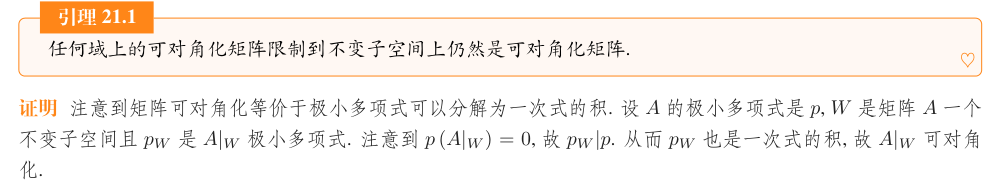
\includegraphics[width=\textwidth]{cmc决赛-2025040617.png}
% \caption{}
\label{}
\end{figure}
\begin{figure}[H]
\centering
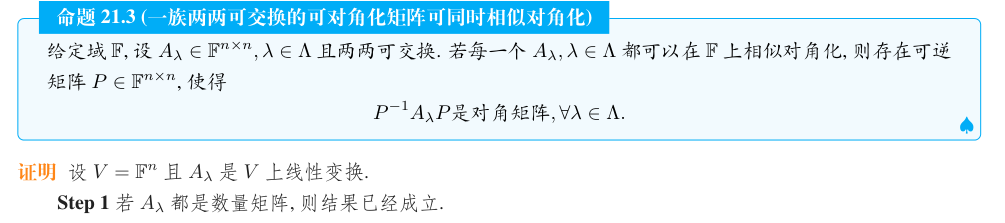
\includegraphics[width=\textwidth]{1-cmc决赛-2025040617.png}
% \caption{}
\label{}
\end{figure}
\begin{figure}[H]
\centering
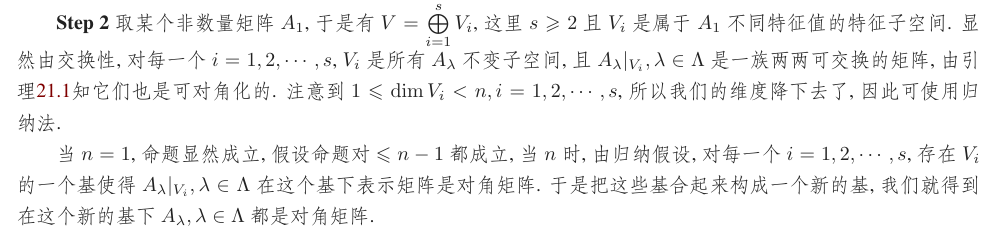
\includegraphics[width=\textwidth]{2-cmc决赛-2025040617.png}
% \caption{}
\label{}
\end{figure}
\begin{figure}[H]
\centering
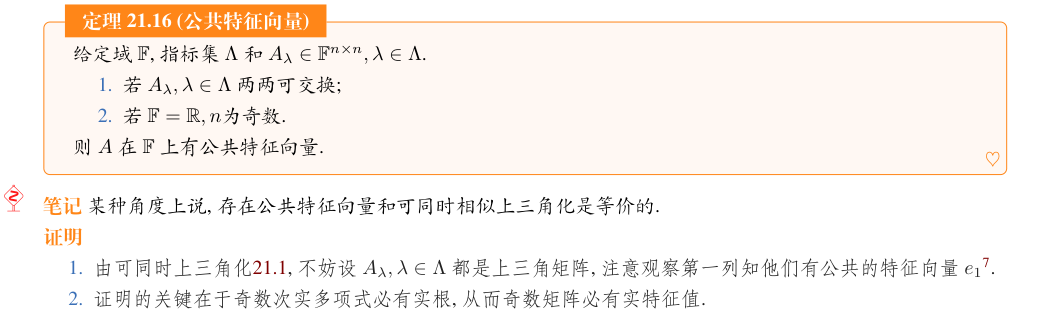
\includegraphics[width=\textwidth]{3-cmc决赛-2025040617.png}
% \caption{}
\label{}
\end{figure}
\begin{figure}[H]
\centering
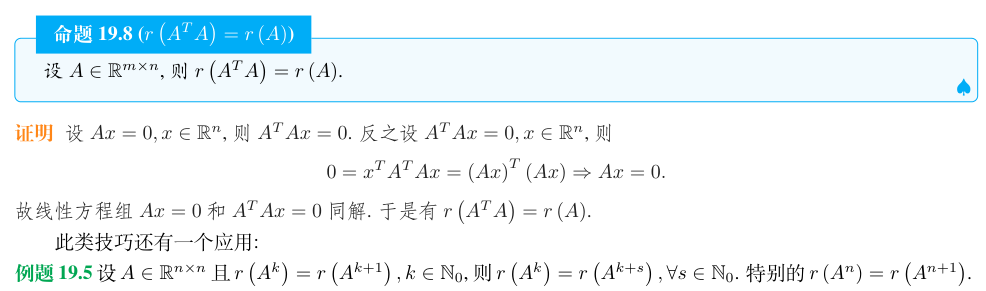
\includegraphics[width=\textwidth]{3-cmc决赛-2025040618.png}
% \caption{}
\label{}
\end{figure}
\begin{figure}[H]
\centering
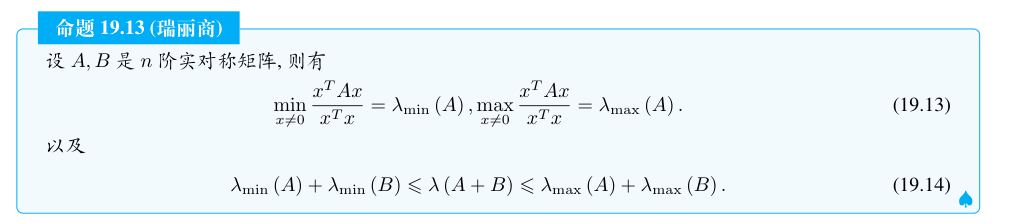
\includegraphics[width=\textwidth]{4-cmc决赛-2025040618.png}
% \caption{}
\label{}
\end{figure}
\begin{figure}[H]
\centering
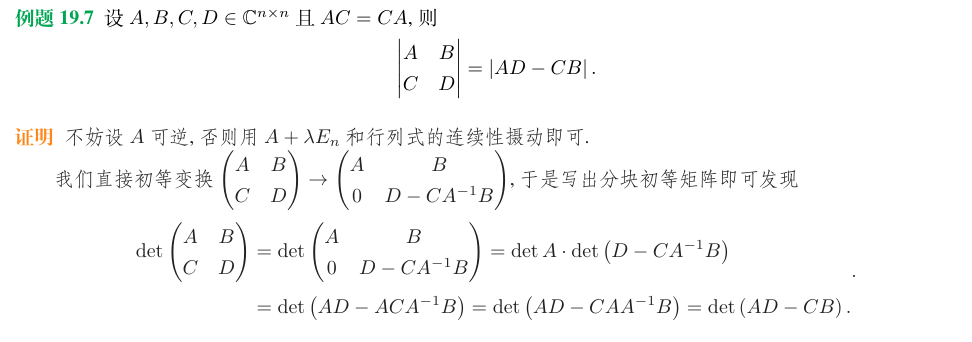
\includegraphics[width=\textwidth]{5-cmc决赛-2025040618.png}
% \caption{}
\label{}
\end{figure}
\begin{figure}[H]
\centering
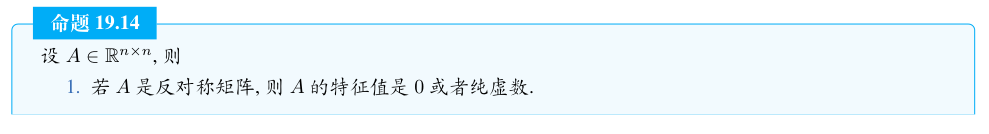
\includegraphics[width=\textwidth]{6-cmc决赛-2025040618.png}
% \caption{}
\label{}
\end{figure}
\begin{figure}[H]
\centering
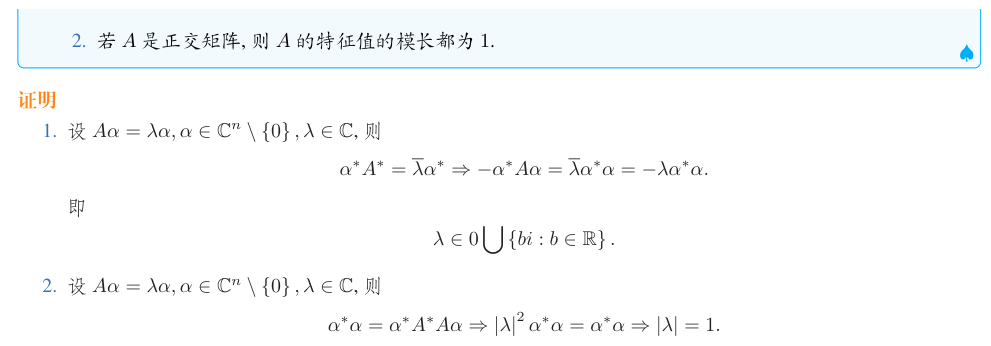
\includegraphics[width=\textwidth]{7-cmc决赛-2025040618.png}
% \caption{}
\label{}
\end{figure}
\begin{figure}[H]
\centering
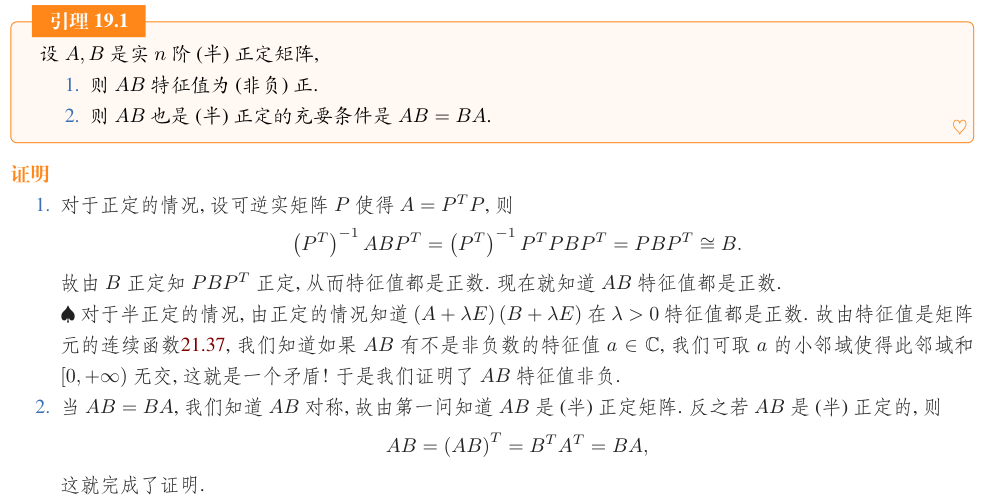
\includegraphics[width=\textwidth]{8-cmc决赛-2025040618.png}
% \caption{}
\label{}
\end{figure}
\begin{figure}[H]
\centering
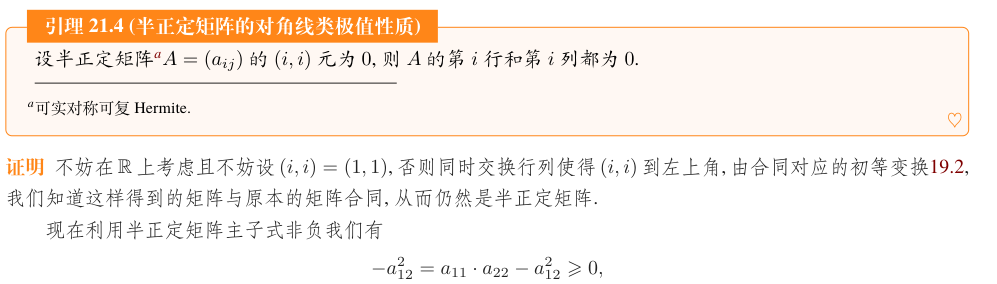
\includegraphics[width=\textwidth]{9-cmc决赛-2025040618.png}
% \caption{}
\label{}
\end{figure}
\begin{figure}[H]
\centering
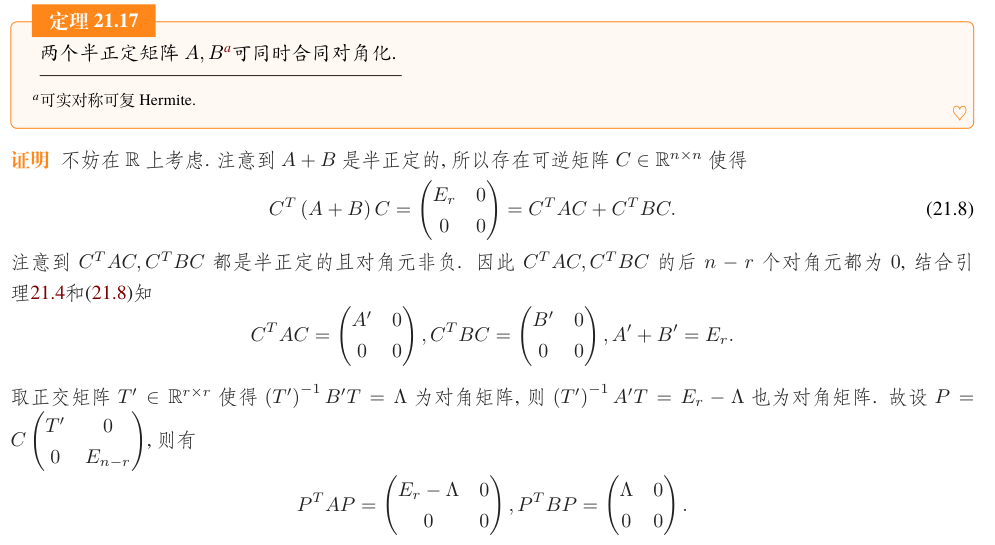
\includegraphics[width=\textwidth]{10-cmc决赛-2025040618.png}
% \caption{}
\label{}
\end{figure}
\begin{figure}[H]
\centering
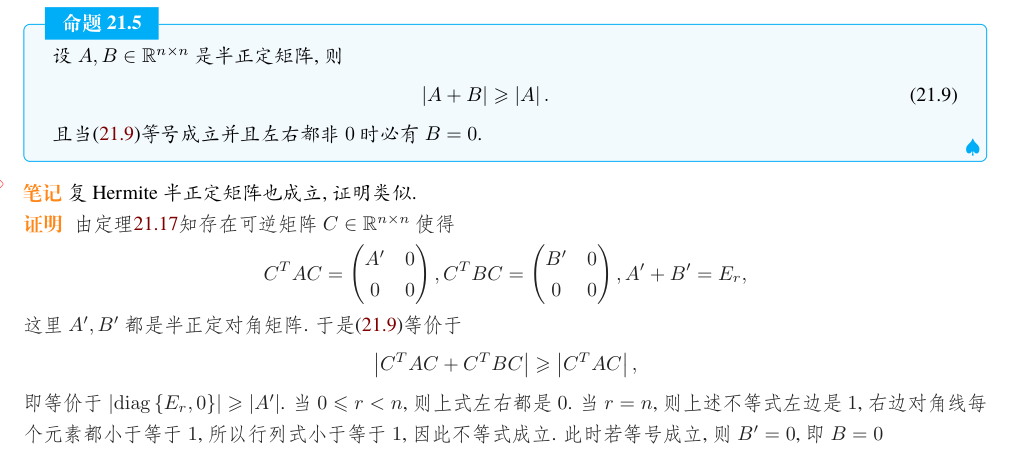
\includegraphics[width=\textwidth]{11-cmc决赛-2025040618.png}
% \caption{}
\label{}
\end{figure}
\begin{figure}[H]
\centering
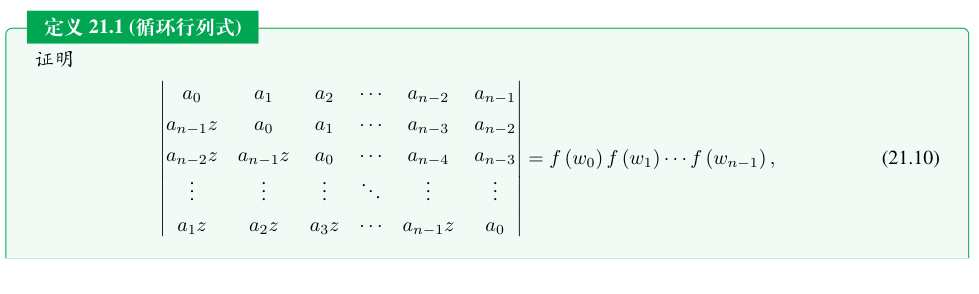
\includegraphics[width=\textwidth]{12-cmc决赛-2025040618.png}
% \caption{}
\label{}
\end{figure}
\begin{figure}[H]
\centering
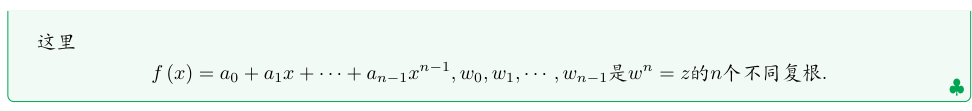
\includegraphics[width=\textwidth]{13-cmc决赛-2025040618.png}
% \caption{}
\label{}
\end{figure}
\begin{figure}[H]
\centering
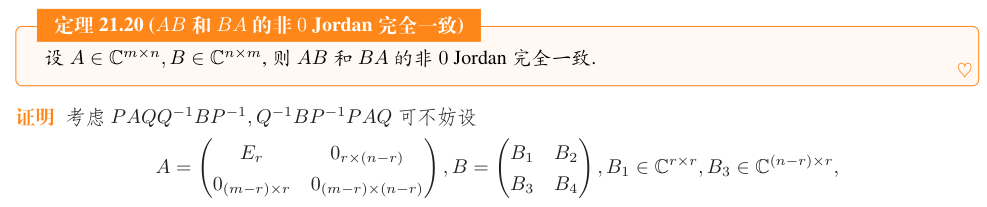
\includegraphics[width=\textwidth]{14-cmc决赛-2025040618.png}
% \caption{}
\label{}
\end{figure}
\begin{figure}[H]
\centering
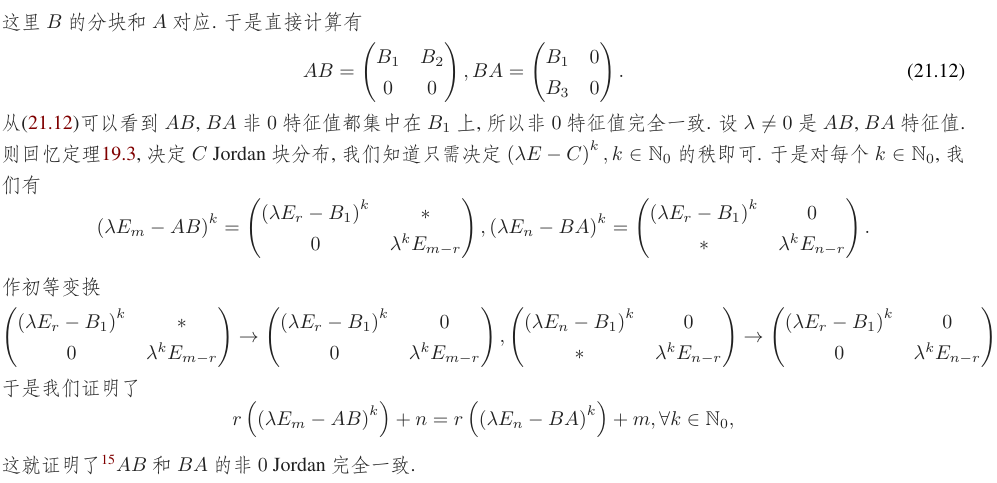
\includegraphics[width=\textwidth]{15-cmc决赛-2025040618.png}
% \caption{}
\label{}
\end{figure}

\begin{figure}[H]
\centering
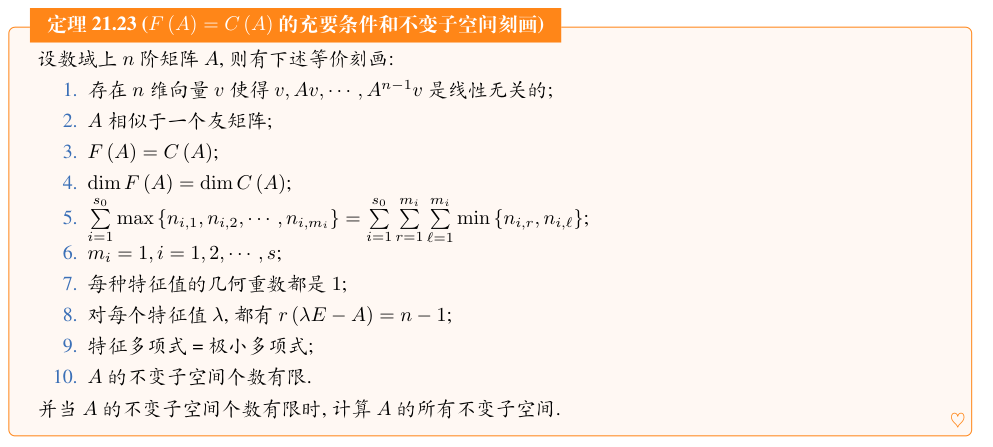
\includegraphics[width=\textwidth]{16-cmc决赛-2025040618.png}
% \caption{}
\label{}
\end{figure}
\begin{figure}[H]
\centering
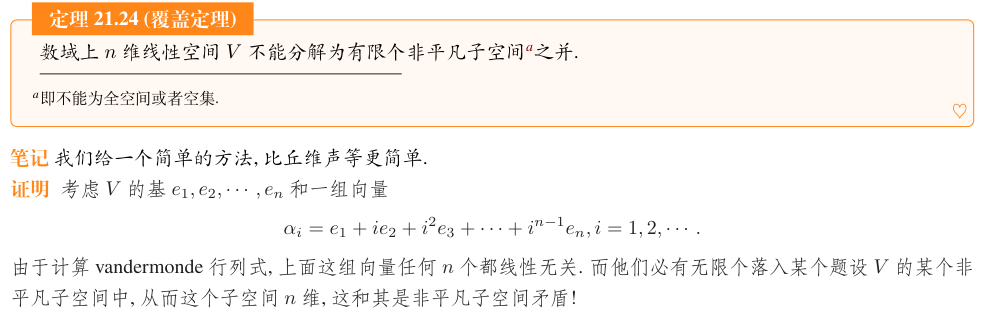
\includegraphics[width=\textwidth]{17-cmc决赛-2025040618.png}
% \caption{}
\label{}
\end{figure}
\begin{figure}[H]
\centering
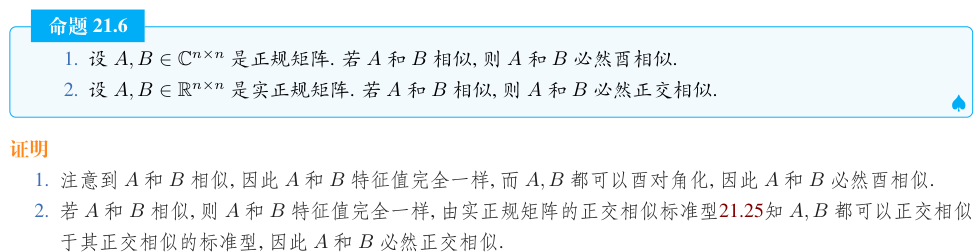
\includegraphics[width=\textwidth]{18-cmc决赛-2025040618.png}
% \caption{}
\label{}
\end{figure}

\section{数学分析}

\subsection{利用 \texorpdfstring{$\delta \epsilon$}{delta epsilon}}


\begin{theorem}
    若$f$在$[1,+\infty)$一致连续且广义可积,则$\lim_{n\to \infty}f(x)=0$.
\end{theorem}

\begin{note}
    $f$的一致连续性是必要的,反例见汪林数分反例第4章最后一个.
\end{note}

\begin{proof}
    $\forall \epsilon>0,\exists \delta>0,s.t.\forall x,y\in [1,+\infty),\left|x-y\right|<\delta\Rightarrow \left|f(x)-f(y)\right|<\epsilon.$ $\exists M>0,s.t.\forall x>M,\left|\int_{x}^{x+\delta}f(x)dx\right|<\textcolor{blue}{\delta\epsilon}.$Then
    $$\delta \left|f(x)\right|\le  \left|\int_{x}^{x+\delta}f(x)dt\right|\le \left|\int_{x}^{x+\delta}f(t)dt\right|+\delta \epsilon\le 2\delta \epsilon\Rightarrow \left|f(x)\right|\le 2\epsilon\Rightarrow \lim_{x\to \infty}f(x)=0.$$
\end{proof}

\begin{note}
    相同的证明思想,利用$\delta \epsilon$,同样出现在$f\in \mathscr{R}[a,b],g\in C[\inf f,\sup f]\Rightarrow g\circ f\in \mathscr{R}[a,b]$中.
\end{note}

\begin{theorem}\label{memeda22}
    $f\in \mathscr{R}[a,b],g\in C[\inf f,\sup f]\Rightarrow g\circ f\in \mathscr{R}[a,b]$
\end{theorem}

\begin{proof}
    $g\in C[a,b]\Rightarrow \forall \epsilon>0,\exists \delta>0,s.t.\forall x,y\in [a,b],\left|x-y\right|<\delta\Rightarrow \left|f(x)-f(y)\right|<\epsilon.$
    \\
    $\displaystyle \exists P=\{x_0,\cdots,x_n\}\ on\ [a,b], \sum_{i=0}^{n}(\sup_{[x_{i-1},x_i]}f-\inf_{[x_{i-1},x_{i}]}f)(x_i-x_{i-1})<\textcolor{blue}{\delta \epsilon}$. Then
    \begin{align*}
        \delta \epsilon
        &\ge \sum_{\left| f\left( x_{i-1} \right) -f\left( x_i \right) \right|\ge \delta}{\left( \underset{\left[ x_{i-1},x_i \right]}{\mathrm{sup}} f-\underset{\left[ x_{i-1},x_i \right]}{\mathrm{inf}} f \right)\left( x_i-x_{i-1} \right)}\\
        &\ge \delta \sum_{\left| f\left( x_{i-1} \right) -f\left( x_i \right) \right|\ge \delta}{\left( x_i-x_{i-1} \right)}\\
        &\Rightarrow \sum_{\left| f\left( x_{i-1} \right) -f\left( x_i \right) \right|\ge \delta}{\left( x_i-x_{i-1} \right)}\le \epsilon
    \end{align*}
    \begin{align*}
        &\sum_{i=0}^{n}\left(\sup_{[x_{i-1},x_i]}g\circ f-\inf_{[x_{i-1},x_{i}]}g\circ f\right)(x_i-x_{i-1})\\
        &\le \sum_{\left| f\left( x_{i-1} \right) -f\left( x_i \right) \right|<\delta}+\sum_{\left| f\left( x_{i-1} \right) -f\left( x_i \right) \right|\ge \delta}{\left( \underset{\left[ x_{i-1},x_i \right]}{\mathrm{sup}}g\circ f-\underset{\left[ x_{i-1},x_i \right]}{\mathrm{inf}}g\circ f \right)\left( x_i-x_{i-1} \right)} \\
        &\le (b-a)\epsilon +2\sup_{[x_{i-1},x_i]} \left|g\right|\epsilon
    \end{align*}
    Hence, $g\circ f\in \mathscr{R}[a,b]$.
\end{proof}

\begin{note}
    $f\in \mathscr{R}[a,b],g\in C[\inf f,\sup f]\nRightarrow f\circ g\in \mathscr{R}[a,b]$. 反例考虑$g$将正测集映到$f$的间断点集合(一个零测集),使得$g\circ f$的间断点集合是正测集,故$f\circ g\notin \mathscr{R}[a,b]$. 只需加强$g$的连续性使得零测集的原像都是零测集.
\end{note}

\subsection{利用单调性两边夹住}

\begin{exercise}
设 $f$ 在 $[0,+\infty)$ 上递增, 对于任何 $T>0, f$ 在 $[0, T]$ 上可积, 且
\begin{align*}
    \lim _{x \rightarrow+\infty} \frac{1}{x} \int_0^x f(t) d t=C .
\end{align*}

证明
\begin{align*}
    \lim _{x \rightarrow+\infty} f(x)=C .
\end{align*}
\end{exercise}

\begin{proof}
    $$\frac{\int_{0}^{x}f(t)dt}{x}\le f(x)\le \frac{\int_{x}^{2x}f(t)dt}{x}=\textcolor{blue}{\frac{\int_{0}^{2x}f(t)dt-\int_{0}^{x}f(t)dt}{x}}$$
    两边取$x\to \infty$得
    $$C\le \lim_{x\to \infty}f(x)\le 2C-C=C\Rightarrow f(x)=C$$
\end{proof}

\begin{exercise}
$f$在$[0,a)$单调,瑕积分$\int_{0}^{a}x^pf(x)dx$收敛,则$\lim_{x\to 0^+}x^{p+1}f(x)=0$.
\end{exercise}

\begin{proof}
    若$p=-1$,则显然$\lim_{x\to 0^+}x^{p+1}f(x)=0$,否则$\int_{0}^{a}x^pf(x)dx$不收敛. 若$p>-1$,不妨设$f$递减,则$\lim_{x\to 0^+}x^pf(x)=+\infty$.
    \begin{align*}
        \int_{0}^{x}t^pf(t)dt\ge \int_{0}^{x}t^pf(x)dt= \frac{1}{p+1}x^{p+1}f(x)\ge \textcolor{blue}{\int_{x}^{2x}t^pf(t)dt}
    \end{align*}
    由柯西收敛,令$x\to 0^+$得
    \begin{align*}
        0\ge\lim_{x\to 0^+}\frac{1}{p+1}x^{p+1}f(x)\ge 0\Rightarrow \lim_{x\to 0^+}\frac{1}{p+1}x^{p+1}f(x)=0.
    \end{align*}
\end{proof}

\begin{exercise}
若$a_n$递减,$\sum_{n=1}^{\infty}a_n$收敛,证明:$\lim_{n\to \infty}na_n=0$
\end{exercise}

\begin{proof}
    \begin{align*}
        0\le na_{2n} \le \textcolor{blue}{\sum_{k=n+1}^{2n}a_k}\to 0(\ as \ n\to \infty) \implies \lim_{n\to \infty}na_n=0
    \end{align*}
\end{proof}

\begin{note}
    注意这里还要补充$a_{2n+1}$这种奇数项的细节. $\lim_{n\to \infty}a_n=0$说明这是显然的.
\end{note}

\subsection{先后取极限}

\begin{exercise}[类似大O Tauber定理]
设$f$在$[a,+\infty)$上恒正,在任意有限区间$[a,b]$可积,且存在常数$M>0$,使得$\int_{a}^{+\infty}f(x)e^{-tx}dx\le M$. 则有$\int_{a}^{+\infty}f(x)dx$收敛.
\end{exercise}

\begin{proof}
    $\forall A>a,$
    \begin{align*}
        M &\ge \int_{a}^{A}f(x)e^{-tx}dx \ge \int_{a}^{A}f(x)(1-tx)dx\\
        &= \int_{a}^{A}f(x)dx-t\int_{a}^{A}xf(x)dx\\
        &\to \int_{a}^{A}f(x)dx\ (as\ t\to 0^+)
    \end{align*}
    因此 $\int_{a}^{+\infty}f(x)dx\le M$. 由单调有界可知$\int_{a}^{+\infty}f(x)dx$收敛.
\end{proof}

\begin{note}
    下面几个定理见《阶的估计基础》chap6
\end{note}

\begin{theorem}[大O Tauber定理]
    \footnote{这是定理\cref{memeda1}的推论}设
    \begin{align*}
        \begin{gathered}
            f(x)=O\left(\frac{1}{x}\right), \\
            F(x)=\int_0^{\infty} e^{-x t} f(t) d t \rightarrow s, \quad x \rightarrow 0+.
        \end{gathered}
    \end{align*}

    则必有
    \begin{align*}
        \int_0^{\infty} f(t) d t=s
    \end{align*}
\end{theorem}

\begin{theorem}
    设 $f(x)$ 为 $(0, \infty)$ 内的非负函数,
    \begin{align*}
        F(x)=\int_0^{\infty} e^{-x t} f(t) d t, \quad x>0 .
    \end{align*}

    若
    \begin{align*}
        F(x) \sim \frac{s}{x^\alpha}, \quad \alpha>0, x \rightarrow 0+
    \end{align*}
    则必有
    \begin{align*}
        \int_0^x f(t) d t \sim \frac{s x^\alpha}{\Gamma(\alpha+1)}, \quad x \rightarrow \infty .
    \end{align*}
\end{theorem}

\begin{corollary}
    设
    \begin{align*}
        a_n \geq 0, \quad \sum_{n=0}^{\infty} a_n x^n \sim \frac{s}{1-x}, \quad x \rightarrow 1-.
    \end{align*}

    则
    \begin{align*}
        \sum_{k=0}^n a_k \sim s n, \quad n \rightarrow \infty .
    \end{align*}
\end{corollary}

\begin{theorem}\label{memeda1}
    设
    \begin{align*}
        \begin{gathered}
            f(x)>-\frac{B}{x}, \quad 0<x<\infty, \\
            F(x)=\int_0^{\infty} e^{-x t} f(t) d t \rightarrow s, \quad x \rightarrow 0+.
        \end{gathered}
    \end{align*}

    则
    \begin{align*}
        \int_0^{\infty} f(t) d t=s .
    \end{align*}
\end{theorem}

\subsection{利用额外的参量}

\begin{exercise}
设 $0 \leqslant a<b$, 是否存在 $f \in C[a, b]$ 使得
$$
    \int_a^b f(x) x^{2 n} \mathrm{~d} x>0, \int_a^b f(x) x^{2 n+1} \mathrm{~d} x<0, n=0,1,2, \cdots .(*)
$$

如果存在, 请给出存在, 如果不存在, 请给出理由.
\end{exercise}

\begin{proof}
    我们考虑 $F(t)=\int_a^b f(x) e^{-x t} d x, \textcolor{blue}{t} \geqslant 0$, 则容易得到
    $$
        |F(t)| \leqslant \max _{[a, b]}|f| \cdot \int_0^{\infty} e^{-x t} d x=\frac{\max _{[a, b]}|f|}{t},
    $$

    即 $\lim _{t \rightarrow+\infty} F(t)=0$.

    但是对任何 $t>0$, 我们都有
    $$
        F(t)=\int_a^b f(x) e^{-x t} d x=\sum_{n=0}^{\infty} \int_a^b f(x) \frac{(-x t)^n}{n!} d x=\sum_{n=0}^{\infty} \frac{(-1)^n t^n}{n!} \int_a^b f(x) x^n d x \stackrel{(*)}{\geqslant} \int_a^b f(x) d x>0 .
    $$

    这就是一个矛盾! 因此我们证明了满足题目条件的 $f$ 不存在.
\end{proof}

\begin{exercise}[反向洛必达]
设 $f \in C[0,+\infty) \cap C^2(0,+\infty)$ 且 $f^{\prime \prime}(x)>-\frac{C}{x^2}$, 则有
$$
    \lim _{x \rightarrow 0^{+}} x f^{\prime}(x)=0 \text {. }
$$
\end{exercise}

\begin{proof}
    不妨设 $C>0$, 对 $h>0$, 由 Taylor 中值定理我们知道存在 $\theta \in(x, x+h)$, 使得
    $$
        f(x+h)=f(x)+f^{\prime}(x) h+\frac{f^{\prime \prime}(\theta)}{2} h^2 .
    $$

    于是
    $$
        f^{\prime}(x)=\frac{f(x+h)-f(x)}{h}-\frac{f^{\prime \prime}(\theta)}{2} h .
    $$

    于是运用条件就有
    $$
        f^{\prime}(x) \leqslant \frac{|f(x+h)-f(x)|}{h}+\frac{C}{2 \theta^2} h \leqslant \frac{|f(x+h)-f(x)|}{h}+\frac{C}{2 x^2} h .
    $$

    我们取 $\textcolor{blue}{h=\eta x, \eta \in(0,1)}$, 就有
    $$
        x f^{\prime}(x) \leqslant x \frac{|f(x+\eta x)-f(x)|}{\eta x}+x \frac{C}{2 x^2} \eta x=\frac{|f(x+\eta x)-f(x)|}{\eta}+\frac{C \eta}{2},
    $$

    因此就有
    $$
        \varlimsup_{x \rightarrow 0^{+}}\left[x f^{\prime}(x)\right] \leqslant \frac{C \eta}{2}
    $$

    由 $\eta$ 任意性可得
    $$
        \varlimsup_{x \rightarrow 0^{+}}\left[x f^{\prime}(x)\right] \leqslant 0 .
    $$

    类似的由 Taylor 中值定理我们知道存在 $\vartheta \in(x-h, x)$, 使得
    $$
        f(x-\eta x)=f(x)-f^{\prime}(x) \eta x+\frac{f^{\prime \prime}(\vartheta)}{2} \eta^2 x^2 .
    $$

    于是
    $$
        \begin{aligned}
            x f^{\prime}(x) & =\frac{f(x)-f(x-\eta x)}{\eta}+\frac{f^{\prime \prime}(\vartheta)}{2} \eta x^2 \geqslant-\frac{|f(x)-f(x-\eta x)|}{\eta}-\frac{C}{2 \vartheta^2} \eta x^2 \\
                            & \geqslant-\frac{|f(x)-f(x-\eta x)|}{\eta}-\frac{C}{2(x-\eta x)^2} \eta x^2=-\frac{|f(x)-f(x-\eta x)|}{\eta}-\frac{C \eta}{2(1-\eta)^2},
        \end{aligned}
    $$

    于是
    $$
        \varliminf_{x \rightarrow 0^{+}}\left[x f^{\prime}(x)\right] \geqslant-\frac{C \eta}{2(1-\eta)^2} \text {. }
    $$

    由 $\eta$ 任意性可得
    $$
        \varliminf_{x \rightarrow 0^{+}}\left[x f^{\prime}(x)\right] \geqslant 0 .
    $$

    因此我们证明了
    $$
        \lim _{x \rightarrow 0^{+}}\left[x f^{\prime}(x)\right]=0 .
    $$
\end{proof}

\subsection{先后两次判断收敛}

\begin{theorem}
    数列$u_n,v_n$单调有界,$\lim_{n\to \infty}u_n=0$,证明:$\sum_{n=1}^{\infty}(-1)^{n-1}u_nv_n$收敛.
\end{theorem}

\begin{proof}
    由狄利克雷判别法:$\sum_{n=1}^{\infty}(-1)^{n-1}u_n$收敛,再由阿贝尔判别法:$\sum_{n=1}^{\infty}(-1)^{n-1}u_nv_n$收敛.
\end{proof}

\subsection{不同意义下的收敛}

\subsubsection{级数收敛}

\begin{definition}
    对于级数$\sum_{n=1}^{\infty}c_n$,记$s_k=\sum_{n=1}^{k}c_n.$
    \begin{itemize}
        \item 普通收敛:$$\lim_{k\to \infty}s_k \ exists$$
        \item Cesàro收敛:$$\lim_{N\to \infty}\sigma_N=\lim_{N\to \infty}\frac{s_1+s_2+\cdots+s_N}{N}\ exists $$
        \item Abel收敛:$$\lim_{r\to 1^-}A(r)=\lim_{r\to 1^-}\sum_{k=0}^{\infty}c_kr^k\ exists$$
    \end{itemize}
\end{definition}

三者的蕴含关系以及反例:

\begin{center}
    \begin{tikzcd}[row sep = tiny, column sep = tiny, font=\small]
        \text{普通收敛} \arrow[rr,Rightarrow,bend left] & \{(-1)^n\}_{n\ge 1} & \text{Cesàro收敛} \arrow[ll,Rightarrow,bend left,"/"{marking} ] \arrow[rr,Rightarrow,bend left] & \{(-1)^{n}n\}_{n\ge 1} & \text{Abel收敛} \arrow[ll,Rightarrow,bend left,"/"{marking} ]\\
        & & & & \\
        D_N(x)=\frac{\sin \left(\left(N+\frac{1}{2}\right) x\right)}{\sin (x / 2)} \arrow[uu,"D_N*f=S_N"description] & & F_N(x)=\frac{1}{N} \frac{\sin ^2(N x / 2)}{\sin ^2(x / 2)} \arrow[uu,"F_N*f=\sigma_N"description] & & P_r(\theta)=\frac{1-r^2}{1-2 r \cos \theta+r^2} \arrow[uu,"P_r*f=\lim_{r\to  1^-}A_f(r)"description]
    \end{tikzcd}
\end{center}

\begin{note}
    下面的级数$\sum_{n=1}^{\infty}c_n$有时代指$f$的傅里叶级数.
\end{note}

\begin{corollary}
    设 $\lim _{n \rightarrow \infty} \sum_{k=1}^n a_k$ 存在, 则
    \begin{align*}
        \lim _{n \rightarrow \infty} \frac{\displaystyle\sum_{k=1}^n k a_k}{n}=0 .
    \end{align*}
\end{corollary}

\begin{note}
    这题不能直接使用Stolz公式.
\end{note}

\begin{proof}
    \begin{align*}
        \lim _{n \rightarrow \infty} \frac{\displaystyle\sum_{k=1}^n k a_k}{n}
         & =
        \lim _{n \rightarrow \infty} \sum_{k=1}^n a_k-\frac{\displaystyle\sum_{k=1}^n (n-k) a_k}{n}   \\
         & =
        \lim _{n \rightarrow \infty} \sum_{k=1}^n a_k-\frac{\displaystyle\sum_{k=1}^n s_k}{n}         \\
         & =
        \lim _{n \rightarrow \infty}\sum_{k=1}^n a_k-\textcolor{blue}{\text{Cesaro mean of }}\sum a_k \\
         & =0                                                                                         \\
    \end{align*}
\end{proof}


\begin{theorem}
    $f$可积,若$f$在$x_0$处连续,则$\lim_{r\to 1^-}A_f(r)(x_0)=f(x_0)$. 若$f$在$x_0$处跳跃间断,则$\lim_{r\to 1^-}A_f(r)(x_0)=\frac{f(x_0^-)+f(x_0^+)}{2}$.
\end{theorem}

\begin{theorem}[Tauber's lemma]
    若$\sum c_n$有Abel收敛到$s$,且$c_n=o(1/n)$\footnote{在Littlewood的版本中,$c_n=O(1/n)$也对,见Stein傅里叶分析p63 exercise 3},则$\sum c_n$收敛到$s$. 即$\lim_{r\to 1^-}\sum c_nr^n=\sum c_n$.
\end{theorem}

\begin{note}
    这可以用来考察收敛半径为1的幂级数在收敛域边界上是否收敛. 若有$c_n=o(1/n)$,则收敛.
\end{note}

\begin{theorem}
    $f$可积,且$\hat{f}(\nu)=O(1/\left|\nu\right|)$,则若$f$在$\theta $连续,则$S_N(f)(\theta)\to f(\theta)\ (as\ N\to \infty)$,若跳跃间断,则$S_N(f)(\theta)\to \frac{f(\theta-)+f(\theta+)}{2}$. 若$f\in C[-\pi ,\pi ]$,则$S_N(f)\to f$ uniformly.
\end{theorem}

% \begin{theorem}[weak version of Littlewood's theorem]
%     $\sum c_n$有Cesaro收敛到$s$,且$c_n=O(1/n)$,则$\sum c_n$收敛到$s$. 
% \end{theorem}

\subsection{傅里叶变换的对称性}

$f$的光滑性与$\hat{f}$的阶:

\begin{center}
    \begin{tikzcd}[row sep = tiny, column sep = tiny, font=\tiny]
        f\in C^k \arrow[r,rightsquigarrow] & \hat{f}=o(1/\left|n\right|^k) & \text{integrate by parts and use Riemann-Lebesgue lemma}\\
        f\text{ is Lipschitz} \arrow[r,rightsquigarrow] & \hat{f}=o(1/\left|n\right|^k) & \text{使用事实\ref{factos}并分段估计}\\
        f\text{ is monotonic} \arrow[r,rightsquigarrow] & \hat{f}=O(1/\left|n\right|) & \text{使用简单函数逼近,或者在实数情况下使用第二积分中值定理}\\
        f\in BV \arrow[r,rightsquigarrow] & \hat{f}=O(1/\left|n\right|) & \text{强行构造分段使用积分第二积分中值定理}\\
        f\ \alpha-\text{Holder连续} \arrow[r,rightsquigarrow] & \hat{f}=O(1/\left|n\right|^\alpha) & \text{使用事实\ref{factos}并分段估计}\\
        f\text{ merely Riemann integrable} \arrow[r,rightsquigarrow] & \hat{f}=o(1) & \text{由Parseval恒等式:}\sum \left|\hat{f}\right|^2=\int_{\mathbb{R}}\left|f\right|^2<\infty\\
    \end{tikzcd}
\end{center}

\begin{property}[factos]\label{factos}
    \begin{align*}
        \hat{f}(n)=-\frac{1}{2 \pi} \int_{-\pi}^\pi f(x+\pi / n) e^{-i n x} d x
    \end{align*}
    hence
    \begin{align*}
        \hat{f}(n)=\frac{1}{4 \pi} \int_{-\pi}^\pi[f(x)-f(x+\pi / n)] e^{-i n x} d x .
    \end{align*}
\end{property}

\subsection{两种方式估阶,阶不同故矛盾}

\begin{note}
    见stein傅里叶分析p117关于Weierstrss函数处处连续但不可导的性质的讨论.
\end{note}

\subsection{反例}

对于$[1,+\infty)$上的正值连续函数$f$,$\sum_{n=1}^{\infty}f(n)$与$\int_{1}^{\infty}f(x)dx$的敛散性互不蕴含.

\begin{note}
    但是对于非负不增函数上面的敛散性是等价的. 这说明非负不增性不能被正值连续性替代. 反例见《实分析中的反例》p113.
\end{note}

级数$\sum_{n=1}^{\infty}a_n$收敛蕴含$\sum_{n=1}^{N}a_n\ (\forall N\in \mathbb{N})$有界且$\lim_{n\to \infty}a_n=0$. 但是反过来不对,有反例,见《实分析中的反例》p103.

级数收敛充要条件(柯西收敛准则)是$\lim_{m,n\to \infty}(a_{n+1}+\cdots+a_{m})=0$,这里$m,n$是无关的. 若$m,n$相关,即$\lim_{n\to \infty}(a_{n+1}+\cdots+a_{m(n)})=0$,则推不出来级数$\sum_{n=1}^{\infty}a_n$收敛,反例考虑调和级数$\sum 1/n$,具体见《实分析中的反例》p106.

% \begin{property}[factos]
%     $$
%     z=\text{Re}(z)-i\text{Re}{iz}
%     $$
% \end{property}

\subsection{隔开边界}

\begin{theorem}[解析函数序列收敛性]\label{ }
    一列调和函数$\displaystyle \{f_n\}_{n=1}^\infty$在 $\displaystyle \Omega$内的紧集上一致收敛到 $\displaystyle f$, 那么 $\displaystyle \{f'_n\}_{n=1}^\infty$在 $\displaystyle \Omega$内的紧集上一致收敛到 $\displaystyle f'$.
\end{theorem}

\begin{proof}
    不妨设 $\displaystyle \{f_n\}_{n=1}^\infty$在 $\displaystyle \Omega$上一致收敛到 $\displaystyle f$. 记$\Omega_\delta=\{z\in \Omega:\overline{D_\delta}(z)\in \Omega\}$. 断言对于$\Omega$内的解析函数$F$,有 $\displaystyle \sup_{z\in \Omega_\delta}\left|F'(z)\right|\leq \frac{1}{\delta}\sup_{\zeta\in \Omega}\left|F(\zeta)\right|$. 于是
    $$
        \sup_{x\in \Omega_\delta}\left|f'(z)-f'_n(z)\right|\leq \frac{1}{\delta}\sup_{\zeta\in \Omega}\left|f(z)-f_n(z)\right|\rightarrow 0(\text{ as }n\to \infty)\ \ \textcolor{blue}{\forall \delta>0}
    $$
    下面证明断言:
    \begin{align*}
        \left|F'(z)\right| & =\left|\frac{1}{2\pi i}\int_{C_\delta(z)} \frac{F(\zeta)}{(\zeta-z)^2 }d\zeta \right|             \\
                           & \leq \frac{1}{2\pi}\int_{C_\delta(z)} \frac{\left|F(\zeta)\right|}{\left|\zeta-z\right|^2 }d\zeta \\
                           & \leq \frac{1}{2\pi} \sup_{\zeta\in \Omega}\left|F(\zeta)\right| \frac{1}{\delta^2}2\pi \delta     \\
                           & =\frac{1}{\delta}\sup_{\zeta\in \Omega}\left|F(\zeta)\right|
    \end{align*}
\end{proof}

\subsection{广义黎曼引理}

\begin{note}
    注意到黎曼引理的证明并不依赖于$g$的周期性,只需要$\displaystyle \lim_{x\to +\infty}\frac{1}{x}\int_{0}^{x}g(t)dt$存在即可.
\end{note}

\begin{theorem}[广义黎曼引理]\label{广义黎曼引理}
    设$f(x)$在$[0,+\infty)$上绝对可积. 有界函数$g(x)$在任意区间上可积且$\displaystyle A=\lim_{x\to +\infty}\frac{1}{x}\int_{0}^{x}g(t)dt$存在,则
    \begin{align*}
        \lim_{\lambda\to \infty}\int_{0}^{\infty}f(x)g(\lambda x)dx=A\int_{0}^{\infty}f(x)dx
    \end{align*}
\end{theorem}

利用广义黎曼引理\cref{广义黎曼引理},我们可以解决下面问题:

\begin{exercise}
设 $f(x) \in C^1[0,+\infty)$, 已知 $\displaystyle \lim _{x \rightarrow+\infty} f(x)=0 、 f(0)=1$, 且 $f^{\prime}(x)$ 在 $[0,+\infty)$ 上绝对可积. 已知部分和有界的序列 $\left\{a_n\right\}(n \in \mathbb{N})$ 的 Cesaro 和为 $A$, 且满足对任意 $\displaystyle t>0, \sum_{n=0}^{\infty} a_n f(t n)$ 都收敛. 证明: $\displaystyle \lim _{t \rightarrow 0^{+}} \sum_{n=0}^{\infty} a_n f(t n)=A$.
\end{exercise}

\subsection{Wiener-Tauberian定理}

\begin{theorem}[Wiener-Tauberian定理]\label{ Wiener-Tauberian定理}
    设 $f(x)$ 是 $\mathbb{R}$ 上的绝对可积函数, 且 $f(x)$ 的 Fourier 变换没有零点,即
    $$
        \widehat{f}(x)=\frac{1}{\sqrt{2 \pi}} \int_{-\infty}^{+\infty} f(t) \mathrm{e}^{-\mathrm{i} x t} \mathrm{~d} t \neq 0, \quad x \in \mathbb{R} .
    $$

    若对于在任意区间上可积,且在 $\mathbb{R}$ 上有界的函数 $h(x)$ 有
    $$
        \lim _{x \rightarrow+\infty} \int_{-\infty}^{+\infty} h(x-t) f(t) \mathrm{d} t=A \int_{-\infty}^{+\infty} f(t) \mathrm{d} t \text {, }
    $$

    那么对任意在 $\mathbb{R}$ 上绝对可积函数 $g(x)$, 会有以下等式
    $$
        \lim _{x \rightarrow+\infty} \int_{-\infty}^{+\infty} h(x-t) g(t) \mathrm{d} t=A \int_{-\infty}^{+\infty} g(t) \mathrm{d} t .
    $$
\end{theorem}

\begin{note}
    这个定理可以用来证明Riemann-Lebesgue引理.
\end{note}

\begin{remark}
    提示: 建议考虑先证明 $\displaystyle \lim _{x \rightarrow+\infty} \int_0^1 \sin (x t) \mathrm{d} t=0$, 然后你会发现上述积分都形如 $\displaystyle F(x)=\int_0^{+\infty} f(t) h(x t) \mathrm{d} t$, 我们可以通过令 $x=\mathrm{e}^u , t=\mathrm{e}^{-s}$, 就可以得到卷积的形式.
\end{remark}

\subsection{求导证明是常数}

例如平均值公式的证明\cref{memeda14}, 例如《微分几何例题详解和习题汇编 by 陈维桓》p30.

\subsection{多项式插值}

\begin{theorem}
    若 $x_0, x_1, \cdots, x_n$ 是不同的实数, 则对任意数值 $y_0, y_1, \cdots, y_n$, 存在唯一的次数至多是 $n$ 次的多项式 $p_n$, 使得
    $$
        p_n\left(x_i\right)=y_i, 0 \leq i \leq n .
    $$
\end{theorem}

\begin{proof}
    唯一性:若$p_n,q_n$都是使得插值成立的至多是 $n$ 次的多项式,则
    \begin{align*}
        (p_n-q_n)(x_i)=0,\ 0\leq i\leq n.
    \end{align*}
    多项式$p_n-q_n$有$n+1$个零点,根据代数基本定理,$p_n-q_n$平凡,即$p_n=q_n$.

    存在性:考虑拉格朗日插值法,直接构造出来插值多项式.
\end{proof}

\begin{theorem}[插值多项式误差定理]\label{插值多项式误差定理}
    若$p(x)$是$f(x)$在点$x_0< x_1< \cdots< x_n$处的插值多项式,则
    \begin{align*}
        p(x)-f(x)=\frac{1}{(n+1)!}f^{(n+1)}(\xi_x)\prod_{i=0}^{n}(x-x_i),\text{其中}\xi_x\in [x_0,x_n]
    \end{align*}
\end{theorem}

\begin{proof}
    证明考虑K值法,直接令$\displaystyle \phi(x)=p(x)-f(x)-K\prod_{i=0}^{n}(x-x_i)$,两边使用$n+1$次罗尔中值定理即可.
\end{proof}

\subsection{证明无穷可微}

\begin{example}
    引理 4. 1 设 $\zeta$ 是这样定义的实函数:
    $$
        \zeta(t)= \begin{cases}\mathrm{e}^{-\frac{1}{t}}, & \text { 对于 } t>0, \\ 0, & \text { 对于 } t \leqslant 0,\end{cases}
    $$

    则 $\zeta \in C^{\infty}(\boldsymbol{R}, \boldsymbol{R})$.
\end{example}

\begin{proof}
    运用 L' Hospital 法则很容易证明对任何多项式 $P(x)$ 都有
    $$
        \lim _{x \rightarrow+\infty} \mathrm{e}^{-x} P(x)=0
    $$

    因而
    $$
        \lim _{t \rightarrow 0+} \mathrm{e}^{-\frac{1}{t}} P\left(\frac{1}{t}\right)=0 .
    $$

    为了证明 $\zeta \in C^{\infty}(\boldsymbol{R}, \boldsymbol{R})$ ,须验证:对任何非负整数 $n$ ,函数 $\zeta(t)$ 在 $t>0$ 范围和 $t \leqslant 0$ 范围分别求出的 $n$ 阶导数都能在 $t=0$处连续地衔接起来。通过归纳,很容易证明 $\zeta$ 的 $n$ 阶导数 $\zeta^{(n)}$ 可以表示为
    $$
        \zeta^{(n)}(t)= \begin{cases}\mathrm{e}^{-\frac{1}{t}} P_n\left(\frac{1}{t}\right), & \text { 对于 } t>0, \\ 0, & \text { 对于 } t \leqslant 0 .\end{cases}
    $$

    这里
    $$
        \begin{aligned}
             & P_0\left(\frac{1}{t}\right)=1,                                                                                                \\
             & P_{n+1}\left(\frac{1}{t}\right)=\left(P_n\left(\frac{1}{t}\right)-P_n^{\prime}\left(\frac{1}{t}\right)\right) \frac{1}{t^2} .
        \end{aligned}
    $$

    因而 $P_n$ 是一个 $2 n$ 次的多项式. 据此可知
    $$
        \lim _{t \rightarrow 0+} \mathrm{e}^{-\frac{1}{t}} P_n\left(\frac{1}{t}\right)=0 .
    $$

    综上所述, 我们证明了 $\zeta \in C^{\infty}(\boldsymbol{R}, \boldsymbol{R})$.
\end{proof}

\subsection{抽象二阶微分方程求解}



\begin{theorem}\label{memeda15}
    考虑如下微分方程:
    \begin{align}
        y^{\prime \prime}+a y^{\prime}+b y=f(x),\ \ \ \ \text{其中}a,b\text{是常数.}
    \end{align}

    它的解为$y(x)=$ 齐通 $\displaystyle +\int_0^x g(x-t) f(t) d t$,其中$g(x)$为$y(0)=0, y'(0)=1$ 的齐次解.
\end{theorem}

\begin{note}
    这个性质可以解决一类微分方程构造问题. 比如证明:
\end{note}

\begin{exercise}
设 $f(x) \in D^2[0,1]$ 满足 $f(0)=2, f^{\prime}(0)=0, f^{\prime}(1)=e-e^{-1}$. 证明存在 $\theta \in(0,1)$, 使得 $f^{\prime \prime}(\theta)=f(\theta)$.
\end{exercise}

\begin{proof}
    \begin{itemize}
        \item \textcolor{red}{若$f''$具有可积性:}考虑微分方程$f''(x)-f(x)=:h(x)$, 其特解为$c_1e^{x}+c_2e^{-x}$,带入定理\cref{memeda15},可知$g(x)=\displaystyle \frac{e^x-e^-x}{2}$. 于是上述微分方程的解为
              \begin{align*}
                  f(x)=c_1e^{x}+c_2e^{-x}+\int_{0}^{x}\frac{e^{x-t}-e^{-x+t}}{2}h(t)dt \\
                  f'(x)=c_1e^{x}-c_2e^{-x}+\int_{0}^{x}\frac{e^{x-t}+e^{-x+t}}{2}h(t)dt
              \end{align*}
              带入初值条件$f(0)=2, f^{\prime}(0)=0$,就有
              \begin{align}\label{memeda16}
                  f(x)=e^{x}+e^{-x}+\int_{0}^{x}\frac{e^{x-t}-e^{-x+t}}{2}h(t)dt
              \end{align}
              再带入$f'(1)=e-e^{-1}$,得到
              \begin{align*}
                  \int_{0}^{1}\frac{e^{1-t}+e^{t-1}}{2}h(t)dt=0,\ \ \ \ \text{其中}\frac{e^{1-t}+e^{t-1}}{2}>0,\forall t\in[0,1].
              \end{align*}
              由积分中值定理:存在$\theta\in (0,1)$,使得
              \begin{align*}
                  h(\theta )\int_{0}^{1}\frac{e^{1-t}+e^{t-1}}{2}dt=0\Rightarrow g(\theta)=0,\ \ \text{即}f^{\prime \prime}(\theta)=f(\theta).
              \end{align*}
        \item \textcolor{red}{若$f''$不具有可积性:}???
    \end{itemize}
\end{proof}

\begin{theorem}[含参积分求导公式]\label{含参积分求导公式}
    对于有定义的积分$\displaystyle f(x)=\int_{a(x)}^{b(x)}g(x,t)dt \displaystyle$,其导数为
    \begin{align}
        f'(x)=\int_{a(x)}^{b(x)}g_x(x,t)dt+g(x,b(x))b'(x)-g(x,a(x))a'(x)
    \end{align}
\end{theorem}

\subsection{等分布}

\begin{theorem}[Weyl等分布定理]\label{Weyl等分布定理}
    用 $\#\{\}$ 表示集合元素个数.

    设 $x_1, x_2, \ldots, x_n, \ldots \in[0,1]$, 如下结果等价:
    \begin{enumerate}
        \item 对任何整数 $k \in \mathbb{N}$ ,有
              $$
                  \lim _{n \rightarrow \infty} \frac{\sum_{j=1}^n e^{2 \pi i k x_j}}{n}=0 .
              $$
        \item 对任何 $f \in C[0,1], f(0)=f(1)$, 有
              $$
                  \lim _{n \rightarrow \infty} \frac{\sum_{j=1}^n f\left(x_j\right)}{n}=\int_0^1 f(x) d x .
              $$
        \item 对任何 $(a, b) \subset[0,1]$ ,有
              $$
                  \lim _{n \rightarrow \infty} \frac{\#\left\{1 \leqslant j \leqslant n: x_j \in(a, b)\right\}}{n}=b-a .
              $$
        \item 对任何 $I \subset[0,1], I$ 是一个区间, 有
              $$
                  \lim _{n \rightarrow \infty} \frac{\#\left\{1 \leqslant j \leqslant n: x_j \in I\right\}}{n}=|I| .
              $$
        \item 对任何 $f \in R[0,1]$, 有
              $$
                  \lim _{n \rightarrow \infty} \frac{\sum_{j=1}^n f\left(x_j\right)}{n}=\int_0^1 f(x) d x .
              $$
    \end{enumerate}
\end{theorem}

\begin{note}
    证明见\href{https://easygl1der.github.io/MyWebsite/Book/exercises.pdf#page=24}{exercises.pdf第24页}
\end{note}

\begin{theorem}[Fejer等分布定理]\label{Fejer等分布定理}
    \begin{enumerate}
        \item 设 $\{f(n)\}_{n \in \mathbb{N}}$ 是 $\mathbb{R}$ 上的实序列, 若存在 $k \in \mathbb{N}$, 使得:
              \begin{enumerate}
                  \item 当 $n$ 充分大时, $\Delta^k f(n)$ \footnote{$\Delta^k$表示k阶差分,$\Delta f(n)=f(n+1)-f(n)$.}严格单调趋近于 0.
                  \item $\displaystyle \lim _{n \rightarrow \infty} n\left|\Delta^k f(n)\right|=+\infty$.
              \end{enumerate}
              则 $\{\{f(n)\}\}_{n \in \mathbb{N}}$ \footnote{$\left\{-\right\}$表示取小数部分.}在 $[0,1)$ 上等分布.
        \item 设 $f: \mathbb{R} \rightarrow \mathbb{R}$ 是足够光滑的函数, 若存在 $k \in \mathbb{N}$, 使得
              \begin{enumerate}
                  \item 当 $x$ 充分大时, $f^{(k)}(x)$ 严格单调趋近于 0.
                  \item $\displaystyle \lim _{x \rightarrow+\infty} x\left|f^{(k)}(x)\right|=+\infty$
              \end{enumerate}
              则 $\{\{f(n)\}\}_{n \in \mathbb{N}}$ 在 $[0,1)$ 上等分布.
    \end{enumerate}
\end{theorem}

\begin{theorem}[Van Der Corput 差分定理]\label{Van Der Corput 差分定理}
    设 $\left\{\xi_n\right\}_{n \in N}$ 是 $[0,1)$ 上的实序列, 若对 $\forall h \in \mathbb{N}$ 都有 $\left\{\xi_{n+h}-\xi_n\right\}_{n \in \mathbb{N}}$ 在 $[0,1)$ 上等分布, 则 $\left\{\xi_n\right\}_{n \in \mathbb{N}}$ 是 $[0,1)$ 上的等分布序列.
\end{theorem}

\begin{note}
    这个定理就是模1等分布,见\href{https://easygl1der.github.io/MyWebsite/Book/exercises.pdf#page=30}{exercises.pdf}
\end{note}

\begin{corollary}
    $\displaystyle \left\{\left\{\frac{n^\alpha}{2 \pi} \right\}\right\}_{n \in \mathbb{N}}$ 在 $[0,1)$ 上等分布,其中$\alpha>0$.
\end{corollary}

\begin{note}
    用一般的Weyl等分布定理\cref{Weyl等分布定理}只能证明$0<\alpha<1$的情况. 见\href{https://easygl1der.github.io/MyWebsite/Book/Stein-I-Fourier%20Analysis.pdf}{Stein傅里叶分析Chapter4 Ex 8}.
\end{note}

\begin{proof}{证明 Van Der Corput 差分定理\cref{Van Der Corput 差分定理}}
    由 Weyl准则可知
    $$
        \lim _{N \rightarrow \infty} \frac{1}{N} \sum_{n=1}^N e^{2 \pi i k\left(\xi_{n+h}-\xi_n\right)}=0, \quad \forall h \in \mathbb{N}, \forall k \in \mathbb{Z} \backslash\{0\}
    $$

    设 $u_n=e^{2 \pi i k \xi_n}$, 则可表示为
    $$
        \lim _{N \rightarrow \infty} \frac{1}{N} \sum_{n=1}^N u_{n+d} \overline{u_n}=0,\text{对于任意}d\in \mathbb{Z}.
    $$
    我们的目标是要证
    $$
        \lim _{N \rightarrow \infty} \frac{1}{N} \sum_{n=1}^N u_n=0
    $$
    对于任意给定的$D\in\mathbb{N}$,由三角不等式:
    \begin{align}
        \left|\frac{1}{N} \sum_{n=1}^N u_n\right| \leq\left|\frac{1}{N} \sum_{n=1}^N u_n-\frac{1}{N} \sum_{n=1}^N \frac{1}{D} \sum_{d=1}^D u_{n+d}\right|+\left|\frac{1}{N D} \sum_{n=1}^N \sum_{d=1}^D u_{n+d}\right|
    \end{align}
    对于第一部分:\footnote{这里用到了重要分析思想,先给定$D$.}
    \begin{align}
        \left|\frac{1}{N} \sum_{n=1}^N u_n-\frac{1}{N} \sum_{n=1}^N \frac{1}{D} \sum_{d=1}^D u_{n+d}\right| \overset{\text{裂项相消}}{=}\frac{1}{N}\left|\sum_{k=1}^D \frac{D+1-k}{D} u_k-\sum_{k=1}^D \frac{D+1-k}{D} u_{N+k}\right| \textcolor{blue}{\overset{D\text{是固定的}}{=}O(\frac{1}{N})}.
    \end{align}
    对于第二部分:
    \begin{align*}
        \left|\frac{1}{N D} \sum_{n=1}^N \sum_{d=1}^D u_{n+d}\right| & \overset{柯西不等式}{\le} \frac{1}{N D} \sqrt{\sum_{n=1}^N 1^2 \sum_{n=1}^N\left|\sum_{d=1}^D u_{n+d}\right|^2} = \sqrt{\frac{1}{D^2}\sum_{d_1,d_2=1}^D{\left( \sum_{n=1}^N{\frac{u_{n+d_1}\overline{u_{n+d_2}}}{N}} \right)}}
        \\
                                                                     & =\sqrt{\frac{1}{D^2}\left[ \sum_{{d_1,d_2=1 \atop {d_1\ne d_2}}}^D{\left( \sum_{n=1}^N{\frac{u_{n+d_1}\overline{u_{n+d_2}}}{N}} \right)}+\sum_{d=1}^D{\left( \sum_{n=1}^N{\frac{u_{n+d}\overline{u_{n+d}}}{N}} \right)} \right]}
        \\
                                                                     & \overset{u_{n+d}\overline{u_{n+d}}=\left|u_{n+d}\right|=1}{=}\sqrt{\frac{1}{D^2}\left[ \sum_{{d_1,d_2=1 \atop {d_1\ne d_2}}}^D{\left( \sum_{n=1}^N{o(1)} \right)}+\sum_{d=1}^D{\left( \sum_{n=1}^N{\frac{1}{N}} \right)} \right]}=\textcolor{blue}{o(1)+\frac{1}{D}}
    \end{align*}
    于是
    \begin{align}
        \left|\frac{1}{N} \sum_{n=1}^N u_n\right|\le O(\frac{1}{N})+o(1)+\frac{1}{D}\longrightarrow \frac{1}{D}(\text{当}N\to \infty)
    \end{align}
    由$D$的任意性可知:
    \begin{align}
        \lim _{N \rightarrow \infty}\left|\frac{1}{N} \sum_{n=1}^N u_n\right|=0
        \implies \lim _{N \rightarrow \infty} \frac{1}{N} \sum_{n=1}^N u_n=0
    \end{align}


    由 Weyl等分布定理\cref{Weyl等分布定理}可知 $\left\{\xi_n\right\}_{n \in \mathbb{N}}$ 是 $[0,1)$ 上的等分布序列.

\end{proof}

\begin{proof}{证明Fejer等分布定理\cref{Fejer等分布定理}}
    \begin{enumerate}
        \item 考虑数学归纳法, 当 $k=1$ 时, 考虑对 $\forall u, v \in \mathbb{R}$, 此时有
              $$
                  \begin{aligned}
                       & \left|e^{2 \pi i u}-e^{2 \pi i v}-2 \pi i(u-v) e^{2 \pi i v}\right|=4 \pi^2\left|\int_0^{u-v}(u-v-\omega) e^{2 \pi i \omega} d \omega\right| \\
                       & \leq 4 \pi^2\left|\int_0^{u-v}(u-v-\omega) d \omega\right|=2 \pi^2(u-v)^2
                  \end{aligned}
              $$

              我们代入 $u=h f(n+1), v=h f(n)$, 其中 $h \in \mathbb{N}$, 由上式可得
              $$
                  \left|\frac{e^{2 \pi i h f(n+1)}}{\Delta f(n)}-\frac{e^{2 \pi i h f(n)}}{\Delta f(n)}-2 \pi i h e^{2 \pi i h f(n)}\right| \leq 2 \pi^2 h^2|\Delta f(n)|, n \in \mathbb{N}
              $$

              由绝对值的三角不等式进一步可得
              $$
                  \begin{aligned}
                       & \left|\frac{e^{2 \pi i h f(n+1)}}{\Delta f(n+1)}-\frac{e^{2 \pi i h f(n)}}{\Delta f(n)}-2 \pi i h e^{2 \pi i h f(n)}\right|                                                                                                 \\
                       & =\left|\left(\frac{e^{2 \pi i h f(n+1)}}{\Delta f(n+1)}-\frac{e^{2 \pi i h f(n+1)}}{\Delta f(n)}\right)+\frac{e^{2 \pi i h f(n+1)}}{\Delta f(n)}-\frac{e^{2 \pi i h f(n)}}{\Delta f(n)}-2 \pi i h e^{2 \pi i h f(n)}\right| \\
                       & \leq\left|\frac{e^{2 \pi i h f(n+1)}}{\Delta f(n+1)}-\frac{e^{2 \pi i h f(n+1)}}{\Delta f(n)}\right|+2 \pi^2 h^2|\Delta f(n)|
                  \end{aligned}
              $$

              于是有
              $$
                  \begin{aligned}
                      \left|2 \pi i h \sum_{n=1}^{N-1} e^{2 \pi i h f(n)}\right| & =\left|\sum_{n=1}^{N-1}\left(2 \pi i h e^{2 \pi i h f(n)}-\frac{e^{2 \pi i h f(n+1)}}{\Delta f(n+1)}+\frac{e^{2 \pi i h f(n)}}{\Delta f(n)}\right)+\frac{e^{2 \pi i h f(n)}}{\Delta f(n)}-\frac{e^{2 \pi i h f(1)}}{\Delta f(1)}\right| \\
                                                                                 & \leq \sum_{n=1}^{N-1}\left|2 \pi i h e^{2 \pi i h f(n)}-\frac{e^{2 \pi i h f(n+1)}}{\Delta f(n+1)}+\frac{e^{2 \pi i h f(n)}}{\Delta f(n)}\right|+\frac{1}{|\Delta f(N)|}+\frac{1}{|\Delta f(1)|}                                        \\
                                                                                 & \leq \sum_{n=1}^{N-1}\left|\frac{1}{\Delta f(n)}-\frac{1}{\Delta f(n+1)}\right|+2 \pi^2 h^2 \sum_{n=1}^{N-1}|\Delta f(n)|+\frac{1}{|\Delta f(N)|}+\frac{1}{|\Delta f(1)|}
                  \end{aligned}
              $$

              注意到 $\Delta f(n)$ 是单调的, 利用交错相消性可知
              $$
                  \left|\frac{1}{N} \sum_{n=1}^{N-1} e^{2 \pi i h f(n)}\right| \leq \frac{1}{\pi|h|}\left(\frac{1}{N|\Delta f(1)|}+\frac{1}{N|\Delta f(N)|}\right)+\frac{\pi|h|}{N} \sum_{n=1}^{N-1}|\Delta f(n)| \xrightarrow{N \rightarrow \infty} 0
              $$

              由 Weyl准则命题得证。
              其它情形下,不妨设 $k \in \mathbb{N}$ ,当 $k+1$ 情形时满足条件,我们有
              $$
                  f(n+h)-f(n)=\sum_{j=0}^{h-1} \Delta f(n+j)
              $$

              于是有
              $$
                  \Delta^k(f(n+h)-f(n))=\sum_{j=0}^{h-1} \Delta^{k+1} f(n+j)
              $$

              由 $\Delta^{k+1} f(n)$ 的单调趋近 0 性质可知, 当 $n$ 充分大时, 于是得 $\Delta^k(f(n+h)-f(n))$ 单调趋近于 0 , 且 $n\left|\Delta^k(f(n+h)-f(n))\right| \rightarrow+\infty$ 重复以上步骤, 得 $\Delta\left(\Delta^{k-1}(f(n+h)-f(n))\right)$单调趋近于 0 , 且
              $$
                  n\left|\Delta\left(\Delta^{k-1}(f(n+h)-f(n))\right)\right| \rightarrow+\infty
              $$

              反复重复差分运算, 将差分次数由 $k+1$ 降低至 1 , 运用 Van Der Corput 差分定理\cref{Van Der Corput 差分定理}最终得 $\{\{f(n)\}\}_{n \in \mathbb{N}}$ 在 $[0,1)$ 上等分布。
        \item 注意到
              $$
                  \Delta f(n)=\int_0^1 f^{\prime}(n+t) d t \quad \Delta^k f(n)=\int_0^1 \int_0^1 \cdots \int_0^1 f^{(k+1)}\left(n+t_1+t_2+\cdots+t_k\right) d t_1 d t_2 \cdots d t_k
              $$

              当 $k=1$ 时, 由 $f^{\prime}(x)$ 单调趋近 0 易知 $\Delta f(n)$ 也单调趋近 0 , 同理易知 $n|\Delta f(n)| \rightarrow+\infty$, 利用 (i) 可知此时命题得证,当 $k+1$ 情形时,有 $\Delta^k f(n)$ 单调趋近于零,且 $n\left|\Delta^k f(n)\right| \rightarrow+\infty$ ,于是利用(i)的结论可知 $\{\{f(n)\}\}_{n \in \mathbb{N}}$ 在 $[0,1)$ 上等分布.

    \end{enumerate}
\end{proof}

\begin{note}
    断言命题对于 $k=1$ 成立. 即若 $\Delta f(n)$ 严格递减趋于 0 (当 $n$ 充分大), 且 $\lim _{n \rightarrow \infty} n|\Delta f(n)|=+\infty$, 就有 $\{\{f(n)\}\}_{n \in \mathbb{N}}$ 在 $[0,1)$ 上等分布.

    现在我们有:
    若 $\Delta^{k+1} f(n)$ 严格递减趋于 0 (当 $n$ 充分大), 且 $\lim _{n \rightarrow \infty} n\left|\Delta^{k+1} f(n)\right|=+\infty$, 则 $\forall h_1 \in \mathbb{N}$, 有 $\Delta^k\left[f\left(n+h_1\right)-f(n)\right]=\Delta^k f\left(n+h_1\right)-\Delta^k f(n)$ 严格递减趋于 0 (当 $n$ 充分大),且 $\left\{\Delta^k f\left(n+h_1\right)\right\}-\left\{\Delta^k f(n)\right\}=\left\{\Delta^k f\left(n+h_1\right)-\Delta^k f(n)\right\}$, 且 $\lim _{n \rightarrow \infty} n\left|\Delta^k f\left(n+h_1\right)-\Delta^k f(n)\right|=+\infty$.记 $f_{h_1}(x)=f\left(x+h_1\right)-f(x)$, 于是 $\Delta^k f_{h_1}(n)$ 严格递减趋于 0 (当 $n$ 充分大),且 $\left\{\Delta^k f\left(n+h_1\right)\right\}-\left\{\Delta^k f(n)\right\}=\left\{\Delta^k f_{h_1}(n)\right\}$, 且 $\lim _{n \rightarrow \infty} n\left|\Delta^k f_{h_1}(n)\right|=+\infty$.
    重复这个过程, 最后 $\Delta f_{h_1, h_2, \cdots, h_k}(n)$ 严格递减趋于 0 (当 $n$ 充分大),且 $\left\{\Delta^k f\left(n+h_j\right)\right\}-\left\{\Delta^k f(n)\right\}=\left\{\Delta^k f_{h_j}(n)\right\} \forall 1 \leq j \leq k$, 且 $\lim _{n \rightarrow \infty} n\left|\Delta f_{h_1, h_2, \cdots, h_k}(n)\right|=+\infty$.于是 $\left\{\left\{f_{h_1, h_2, \cdots, h_k}(n)\right\}\right\}_{n \in \mathbb{N}}$ 在 $[0,1)$ 上等分布。应用 $k$ 次 Van Der Corput差分定理\cref{Van Der Corput 差分定理}: $\left\{\left\{f_{h_1, h_2, \cdots, h_{k-1}}(n)\right\}\right\}_{n \in \mathbb{N}}$ 在 $[0,1)$ 上等分布 $\ldots . .\{\{f(n)\}\}_{n \in \mathbb{N}}$ 在 $[0,1)$ 上等分布.
\end{note}

\subsection{利用任意性}

在解析数论中,定义$\displaystyle \psi(x)=\sum_{p^m\le x}\log p=\sum_{p\le x}\left[\frac{\log x}{\log p}\right]\log p$, $\displaystyle \pi (x)=\sum_{p\le x}1$.

\begin{theorem}
    若$\psi(x)\sim x(x\to\infty)$, 则$\pi (x)\sim x/\log x(x\to \infty)$.
\end{theorem}

\begin{proof}
    一方面,
    \begin{align}\label{memeda20}
        \psi(x)=\sum_{p\le x}\left[\frac{\log x}{\log p}\right]\log p\le \sum_{p\le x}\log x=\pi (x)\log x\implies \frac{\psi(x)}{x}\le \frac{\pi(x)\log x}{x},\forall x\in \mathbb{R}
    \end{align}
    另一方面,\textcolor{blue}{对于任意给定的$0<\alpha<1$ }
    \begin{align*}
        \psi(x)\ge \sum_{p\le x}\log p\ge \sum_{x^\alpha<p\le x}\log p\ge (\pi(x)-\pi(x^\alpha))\log x^\alpha\implies \psi(x)+\alpha\pi (x^\alpha)\log x\ge \alpha\pi(x)\log x
    \end{align*}
    于是
    \begin{align*}
        \frac{\psi(x)}{x}+\alpha\frac{\log x}{x^{1-\alpha}}\ge \frac{\psi(x)}{x}+\alpha\frac{\pi(x^\alpha)\log x}{x}\ge \alpha \frac{\pi(x)\log x}{x}\implies \limsup_{x\to \infty}\frac{\psi(x)}{x}\ge \alpha\limsup_{x\to \infty}\frac{\pi(x)\log x}{x}
    \end{align*}
    由$\alpha $任意性
    \begin{align*}
        1=\textcolor{blue}{\limsup_{x\to \infty}\frac{\psi(x)}{x}\ge  \limsup_{x\to \infty}\frac{\pi(x)\log x}{x}}\ge \liminf_{x\to \infty}\frac{\pi(x)\log x}{x}\overset{\cref{memeda20}}{\ge} \liminf_{x\to \infty}\frac{\psi(x)}{x}=1
    \end{align*}

\end{proof}

\subsection{求和下的大O小o估阶}

\begin{proposition}
    设 $b_n>0$, 且 $a_n=O\left(b_n\right), n \rightarrow \infty$, 则

    $$
        \sum_{n=1}^N a_n=O\left(\sum_{n=1}^N b_n\right), \quad N \rightarrow \infty
    $$

\end{proposition}

\begin{note}
    此证明相当显然.
\end{note}

\begin{proof}
    存在常数$C>0,N>0$,使得$\left|a_n\right|<C\cdot b_n,\forall n\ge N$.

    只需要验证存在常数$C'>0$,使得$\displaystyle \left|\sum_{k=1}^{n}a_k\right|\le C'\sum_{k=1}^{n}b_k,\forall n>N.$ 这只需要如下的简单放缩:

    \begin{align*}
        \left|\sum_{k=1}^{n}a_k\right| &=\left|\sum_{k=1}^{N}a_k\right|+\left|\sum_{k=N+1}^{n}a_k\right| \\
        &=\left|\sum_{k=1}^{N}\frac{a_k}{b_k}b_k\right|+\left|\sum_{k=N+1}^{n}a_k\right| \\
        &\le \sup_{1\le k\le N}\frac{\left|a_k\right|}{b_k}\sum_{k=1}^{N}b_k+C \sum_{k=N+1}^{n}b_k \\
        &\le \left(C+\sup_{1\le k\le N}\frac{\left|a_k\right|}{b_k}\right)\sum_{k=1}^{n}b_k
    \end{align*}
\end{proof}

\begin{proposition}
    设 $b_n>0, \textcolor{brown}{\displaystyle\sum_{n=1}^{\infty} b_n=\infty}$, 且 $a_n=o\left(b_n\right), n \rightarrow \infty$, 则

    $$
        \sum_{n=1}^N a_n=o\left(\sum_{n=1}^N b_n\right), \quad N \rightarrow \infty
    $$

\end{proposition}

\begin{note}
    这里的证明要在$N$上做手脚.
\end{note}

\begin{proof}
    对于任意给定的$\varepsilon>0$,存在$N>0$,使得$a_n\le \displaystyle\frac{\varepsilon}{2} \cdot b_n,\forall n\ge N$,\textcolor{brown}{还存在$N'>0$},使得$\displaystyle\sum_{k=1}^{N}b_k\le \displaystyle\frac{\varepsilon}{2 \displaystyle \sup_{1\le k\le N}\frac{\left|a_k\right|}{b_k}} \displaystyle\sum_{k=1}^{n}b_k,\forall n>N'$.

    只需要验证$\forall \varepsilon>0$,使得$\displaystyle \left|\sum_{k=1}^{n}a_k\right|\le \varepsilon\sum_{k=1}^{n}b_k,\forall n>N'.$ 这只需要如下的简单放缩:

    \begin{align*}
        \left|\sum_{k=1}^{n}a_k\right| &=\left|\sum_{k=1}^{N}a_k\right|+\left|\sum_{k=N+1}^{n}a_k\right| \\
        &=\left|\sum_{k=1}^{N}\frac{a_k}{b_k}b_k\right|+\left|\sum_{k=N+1}^{n}a_k\right| \\
        &\le \sup_{1\le k\le N}\frac{\left|a_k\right|}{b_k}\sum_{k=1}^{N}b_k+\displaystyle\frac{\varepsilon}{2} \sum_{k=N+1}^{n}b_k \\
        &\le \displaystyle\frac{\varepsilon}{2} \displaystyle\sum_{k=1}^{n}b_k+\frac{\varepsilon}{2} \sum_{k=N+1}^{n}b_k \\
        &\le \varepsilon \displaystyle\sum_{k=1}^{n}b_k
    \end{align*}
\end{proof}

\begin{remark}
    此证明还可见于《阶的估计基础》p18 定理2,其中采用了大O小o的语言来书写证明,比较抽象.
\end{remark}

\subsection{利用一致收敛性}

定理\cref{memeda22}就是一个例子,下面还有另一个例子:

\begin{theorem}{Bernstein多项式逼近}
    $f$是$[0,1]$上的连续函数,则其Bernstein多项式$B_n(f)$在$C[0,1]$上一致收敛于$f$. 其中
    $$
    B_n(f)(x)=\sum_{k=0}^{n}f\left(\frac{k}{n}\right)C_{n}^{k}x^k(1-x)^{n-k}
    $$
    也就是说
    $$
    \lim_{n\to \infty}\sup_{x\in [0,1]}\left|B_n(f)(x)-f(x)\right|=0
    $$
\end{theorem}


\begin{note}
    从概率论的角度给出证明,这样更好地给出了Bernstein多项式的构造思路. 来源于\href{https://easygl1der.github.io/MyWebsite/Book/PTE5_011119.pdf#page=66}{Durrett}.
\end{note}

\begin{proof}
    考虑$n$个独立随机变量$X_i$,且$P(X_i=1)=p,P(X_i=0)=1-p$,有$EX_i=p,Var(X_i)=p(1-p)$,令$S_n=X_1+X_2+\cdots+X_n$,就有
    $$
    P(S_n=m)=C_{n}^{m}p^m(1-p)^{n-m}
    $$ 
    于是$Ef(S_n/n)=B_n(f)(p)$. 由Durrett Theorem 2.2.3,$S_n/n$依概率收敛于$p$. 结合Theorem 2.2.3的证明和$p(1-p)\le \frac{1}{4},\forall p\in [0,1]$,有
    $$
    P(\lvert S_n/n-p\rvert\ge \delta)\le \frac{var(S_n/n)}{\delta^2}= \frac{p(1-p)}{n\delta^2} \le \frac{1}{4n\delta^2}
    $$
    为了证明$Ef(S_n/n)\to f(p)$,由于$f$在$[0,1]$上一致连续,对于任意$\varepsilon>0$,存在$\delta>0$,使得当$\left|x-y\right|<\delta$时,$\left|f(x)-f(y)\right|<\varepsilon$。使用 Jensen不等式 \cref{Jensen不等式}就有
    $$
    \begin{aligned}
        \lvert Ef(S_n/n)-f(p)\rvert & \overset{\cref{Jensen不等式}}{\le} E\lvert f(S_n/n)-f(p)\rvert = \int\lvert f(S_n/n)-f(p)\rvert dP\\
        & =\int_{\{\lvert S_n/n-p\rvert\le \delta\}}\lvert f(S_n/n)-f(p)\rvert dP+\int_{\{\lvert S_n/n-p\rvert>\delta\}}\lvert f(S_n/n)-f(p)\rvert dP\\
        & \le \varepsilon P(\lvert S_n/n-p\rvert\le \delta)+\sup_{[0,1]}\lvert f(x)-f(p)\rvert P(\lvert S_n/n-p\rvert>\delta)\\
        & \le \varepsilon + 2 \sup_{x\in [0,1]}\lvert f(x)\rvert \frac{1}{4n\delta^2}
    \end{aligned}
    $$
    令$n\to\infty$,就有$\limsup_{n\to \infty}\lvert Ef(S_n/n)-f(p)\rvert\le \varepsilon$. 由$\varepsilon$的任意性,即有$\limsup_{n\to \infty}\lvert Ef(S_n/n)-f(p)\rvert=0$,即$Ef(S_n/n)\to f(p)$.
\end{proof}

\begin{theorem}[Jensen不等式]\label{Jensen不等式}
    若$\varphi$是凸函数\footnote{即$\forall x,y\in \mathbb{R}$,有$\theta \varphi(x)+(1-\theta)\varphi(y)\le \varphi(\theta x+(1-\theta)y)$,其中$0\le \theta\le 1$.},则$ E\varphi(X)\ge \varphi(EX)$.
\end{theorem}

\begin{theorem}[Markov不等式]\label{Markov不等式}
    设$X$是随机变量,则对任意$a>0$,有$P(\lvert X\rvert\ge a)\le \frac{E\lvert X\rvert}{a}$.
\end{theorem}

\begin{proof}
    由$X$的非负性,有$E\lvert X\rvert=\int_0^{\infty}P(\lvert X\rvert\ge t)dt\ge \int_0^aP(\lvert X\rvert\ge t)dt\ge aP(\lvert X\rvert\ge a)$,即$P(\lvert X\rvert\ge a)\le \frac{E\lvert X\rvert}{a}$.
\end{proof}

\subsection{多元函数}

\begin{theorem}[含参积分求导公式]
    设$f(x,y)$与$D_2f(x,y)$在矩形$[a,b]\times [c,d]$上连续,设$p(x),q(x)$在$[a,b]$上可微,且$\forall y\in[c,d]$,有$p(y),q(y)\in [a,b]$,则
    $$
    \frac{d}{dx}\int_{p(y)}^{q(y)}f(x,y)dx=-f(p(y),y)p'(y)+f(q(y),y)q'(y)+\int_{p(y)}^{q(y)}D_2f(x,y)dx
    $$
\end{theorem}

\begin{proof}
    设$G(x_1,x_2,x_3)=\int_{x_1}^{x_2}f(t,x_3)dt$,考虑$F(y)=G(p(y),q(y),y)$作为复合函数,由链式法则得到
    $$
    F'(y)=D_1G(p(y),q(y),y)p'(y)+D_2G(p(y),q(y),y)q'(y)+D_3G(p(y),q(y),y)
    $$
    我们有$D_1G(x_1,x_2,x_3)=-f(x_1,x_3),D_2G(x_1,x_2,x_3)=f(x_2,x_3),D_3G(x_1,x_2,x_3)=\int_{x_1}^{x_2}D_2f(t,x_3)dt$,于是
    $$
    F'(y)=-f(p(y),y)p'(y)+f(q(y),y)q'(y)+\int_{p(y)}^{q(y)}D_2f(t,y)dt
    $$
\end{proof}

\subsection{函数方程}

\href{https://easygl1der.github.io/MyWebsite/Book/Functional%20equations%20and%20inequalities%20with%20applications%20(Palaniappan%20Kannappan%20(auth.))%20(Z-Library).pdf#page=24}{Cauchy函数方程}

\section{高等代数}

\subsection{实矩阵、正规、对称}

\begin{center}
    \begin{tikzcd}[column sep = small, row sep = small, font=\tiny]
        & \text{\tiny 实特征值一定有对应实特征向量\cref{memeda3}} \arrow[ld]\arrow[rdd,"\text{\tiny 有实特征值}"description]  & \text{\tiny 复特征值和特征向量变成二阶块} \arrow[dd,"\text{\tiny 实与复的桥梁\cref{memeda8}}"near start,"\text{\tiny 没实特征值}"description]\\
        \text{\tiny 实对称正交相似对角化的几何证明\cref{memeda12}} \arrow[d]&  &  \\
        \text{\tiny 实对称正交相似对角化\cref{memeda9}} & \text{\tiny 实正规矩阵标准型\cref{memeda2}} \arrow[l] &\text{\tiny 实方阵标准型\cref{例 9.87}} \arrow[l,"\text{\tiny 正规矩阵有分块对角形式\cref{例 9.89}}"] \\
        \text{\tiny 特征值全是实数\cref{memeda11}} \arrow[u] \arrow[d]   \arrow[uu,bend left=80]& & \\
        \text{\tiny Hermite矩阵} & \text{\tiny 复正规矩阵酉相似于对角阵\cref{memeda10}} \arrow[uu,"\text{\tiny 实与复的桥梁\cref{memeda8}}"] \arrow[l,"\text{\tiny 若特征值全为实数\cref{memeda13}}"] & \text{\tiny 复方阵酉相似上三角化(Schur定理\cref{Schur定理})} \arrow[uu,"\text{\tiny 实与复的桥梁\cref{memeda8}}"] \arrow[l,bend left,"\mathbb{C}\text{\tiny 是代数闭域}",no head]\arrow[l,"{\tiny AA^*=A^*A}"] \\
    \end{tikzcd}
\end{center}

\begin{theorem}\label{memeda2}
    实正规矩阵可以正交相似为标准型.
\end{theorem}

\begin{theorem}\label{memeda9}
    实对称矩阵可正交相似对角化.
\end{theorem}

\begin{theorem}[Schur定理]\label{Schur定理}
    设 $V$ 是 $n$ 维酉空间, $\varphi$ 是 $V$ 上的线性算子, 则存在 $V$ 的一组标准正交基, 使 $\varphi$ 在这组基下的表示矩阵为上三角阵.
\end{theorem}

\begin{proof}
    选取$\varphi$的一个单位特征向量,再扩充成$V$的一组标准正交基,归纳得证.
\end{proof}

\begin{theorem}\label{memeda10}
    复矩阵 $\boldsymbol{A}$ 为复正规矩阵的充分必要条件是 $\boldsymbol{A}$ 酉相似于对角阵.
\end{theorem}

\begin{note}
    实对称矩阵一定是实正规矩阵,于是考虑正交相似标准型,这个正交相似标准型还要是对称的,故斜对角线上的$b_i=0,\forall i$,于是是对角阵.
\end{note}

\begin{property}[factos]
    在内积空间中平行四边形两对角线平方和等于四边平方和, 即
    \begin{align*}
        \|\boldsymbol{\alpha}+\boldsymbol{\beta}\|^2+\|\boldsymbol{\alpha}-\boldsymbol{\beta}\|^2=2\|\boldsymbol{\alpha}\|^2+2\|\boldsymbol{\beta}\|^2 .
    \end{align*}
\end{property}

\begin{definition}[伴随$(\varphi(\alpha),\beta)=(\alpha,\varphi^*(\beta))$]
    设 $V$ 是 $n$ 维内积空间, $\left\{e_1, e_2, \cdots, e_n\right\}$ 是 $V$ 的一组标准正交基. 若 $V$ 上的线性算子 $\varphi$ 在这组基下的表示矩阵为 $A$, 则当 $V$ 是酉空间时, $\varphi^*$\footnote{$\forall \alpha,\beta\in V,(\varphi(\alpha),\beta)=(\alpha,\varphi^*(\beta)).$}在同一组基下的表示矩阵为 $\bar{A}^{\prime}$, 即 $A$ 的共轭转置; 当 $V$ 是欧氏空间时, $\varphi^*$ 的表示矩阵为 $\boldsymbol{A}^{\prime}$, 即 $\boldsymbol{A}$ 的转置.
\end{definition}

\begin{definition}[保持内积的线性变换$(\varphi(\alpha),\varphi (\beta))=(\alpha,\beta)$]
    设 $\varphi$ 是内积空间 $V$ 上保持内积的线性变换\footnote{$\forall \alpha,\beta\in V,(\varphi(\alpha),\varphi (\beta))=(\alpha,\beta).$}, 若 $V$ 是欧氏空间,则称 $\varphi$ 为正交变换或正交算子\footnote{在欧式空间任意一组标准正交基下表示矩阵为正交矩阵$A$,$AA^T=I$.}; 若 $V$ 是酉空间,则称 $\varphi$ 为酉变换或酉算子\footnote{在酉空间任意一组标准正交基下表示矩阵为酉矩阵$U$,$UU^*=I$.}.
\end{definition}

\begin{definition}[自伴随算子$\varphi^*=\varphi$]
    设 $\varphi$ 是内积空间 $V$ 上的线性变换, $\varphi^*$ 是 $\varphi$ 的伴随, 若 $\varphi^*=\varphi$,则称 $\varphi$ 是自伴随算子. 当 $V$ 是欧氏空间时, $\varphi$ 也称为对称算子或对称变换\footnote{在欧式空间任意一组标准正交基下表示矩阵为对称矩阵$A$,$A=A^T$.}; 当 $V$是酉空间时, $\varphi$ 也称为 Hermite 算子或 Hermite 变换\footnote{在酉空间任意一组标准正交基下表示矩阵为Hermite矩阵$A$,$A=A^*$.}.
\end{definition}

\begin{definition}[正规算子]
    设 $\varphi$ 是内积空间 $V$ 上的线性变换, $\varphi^*$ 是其伴随, 若 $\varphi \varphi^*=\varphi^* \varphi$,则称 $\varphi$ 是 $V$ 上的正规算子. 为了不引起混淆, 我们也称酉空间 (欧氏空间) $V$ 上的正规算子 $\varphi$ 为复正规算子 (实正规算子). 复矩阵 $A$ 若适合 $\bar{A}^{\prime} A=A \bar{A}^{\prime}$, 则称其为复正规矩阵. 实矩阵 $\boldsymbol{A}$ 若适合 $\boldsymbol{A}^{\prime} \boldsymbol{A}=\boldsymbol{A} \boldsymbol{A}^{\prime}$, 则称其为实正规矩阵.
\end{definition}

\begin{theorem}\label{memeda11}
    设 $V$ 是 $n$ 维酉空间, $\varphi$ 是 $V$ 上的自伴随算子, 则 $\varphi$ 的特征值全是实数且属于不同特征值的特征向量互相正交.
\end{theorem}

\begin{proof}
    证明 设 $\lambda$ 是 $\varphi$ 的特征值, $x$ 是属于 $\lambda$ 的特征向量, 则
    \begin{align*}
        \begin{aligned}
            \lambda(\boldsymbol{x}, \boldsymbol{x}) & =(\lambda \boldsymbol{x}, \boldsymbol{x})=(\boldsymbol{\varphi}(\boldsymbol{x}), \boldsymbol{x})=\left(\boldsymbol{x}, \varphi^*(\boldsymbol{x})\right) \\
                                                    & =(\boldsymbol{x}, \boldsymbol{\varphi}(\boldsymbol{x}))=(\boldsymbol{x}, \lambda \boldsymbol{x})=\bar{\lambda}(\boldsymbol{x}, \boldsymbol{x}) .
        \end{aligned}
    \end{align*}

    因为 $(\boldsymbol{x}, \boldsymbol{x}) \neq 0$, 故 $\bar{\lambda}=\lambda$, 即 $\lambda$ 是实数. 又若设 $\mu$ 是 $\varphi$ 的另一个特征值, $\boldsymbol{y}$ 是属于 $\mu$ 的特征向量, 注意到 $\lambda, \mu$ 都是实数, 故有
    \begin{align*}
        \begin{aligned}
            \lambda(\boldsymbol{x}, \boldsymbol{y}) & =(\lambda \boldsymbol{x}, \boldsymbol{y})=(\boldsymbol{\varphi}(\boldsymbol{x}), \boldsymbol{y})=\left(\boldsymbol{x}, \varphi^*(\boldsymbol{y})\right) \\
                                                    & =(\boldsymbol{x}, \boldsymbol{\varphi}(\boldsymbol{y}))=(\boldsymbol{x}, \mu \boldsymbol{y})=\mu(\boldsymbol{x}, \boldsymbol{y})
        \end{aligned}
    \end{align*}

    由于 $\lambda \neq \mu$, 故 $(\boldsymbol{x}, \boldsymbol{y})=0$, 即 $\boldsymbol{x} \perp \boldsymbol{y}$.
\end{proof}

\begin{note}
    推论是实(复)对称矩阵的特征值全为实数,不同特征值的特征向量两两正交.
\end{note}

\begin{theorem}[实对称正交相似对角化的几何证明]\label{memeda12}
    设 $V$ 是 $n$ 维内积空间, $\varphi$ 是 $V$ 上的自伴随算子, 则存在 $V$ 的一组标准正交基, 使 $\varphi$ 在这组基下的表示矩阵为实对角阵, 且这组基恰为 $\varphi$ 的 $n$个线性无关的特征向量.
\end{theorem}

\begin{proof}
    证明 首先需要说明的是, 若 $V$ 是欧氏空间, 则由于自伴随算子 $\varphi$ 的特征值都是实数, 故有实的特征向量. 不妨设 $u$ 是 $\varphi$ 的特征向量, 令 $v_1=\frac{u}{\|u\|}$, 则 $v_1$ 是 $\varphi$ 的长度等于 1 的特征向量. 我们对维数 $n$ 用归纳法.

    若 $\operatorname{dim} V=1$, 结论已成立. 设对小于 $n$ 维的内积空间结论成立. 令 $W$ 为由 $v_1$ 张成的子空间, $W^{\perp}$ 为 $W$ 的正交补空间, 则 $W$ 是 $\varphi$ 的不变子空间且
    \begin{align*}
        V=W \oplus W^{\perp}, \quad \operatorname{dim} W^{\perp}=n-1 .
    \end{align*}
    由命题 9.3.1 可知 $W^{\perp}$ 是 $\varphi^*=\varphi$ 的不变子空间. 将 $\varphi$ 限制在 $W^{\perp}$ 上仍是自伴随算子. 由归纳假设, 存在 $W^{\perp}$ 的一组标准正交基 $\left\{v_2, \cdots, v_n\right\}$, 使 $\varphi$ 在这组基下的表示矩阵为实对角阵, 且 $\left\{\boldsymbol{v}_2, \cdots, \boldsymbol{v}_n\right\}$ 是其特征向量. 因此, $\left\{\boldsymbol{v}_1, \boldsymbol{v}_2, \cdots, \boldsymbol{v}_n\right\}$ 构成了 $V$ 的一组标准正交基, $\boldsymbol{\varphi}$ 在这组基下的表示矩阵为实对角阵, 且 $\left\{\boldsymbol{v}_1, \boldsymbol{v}_2, \cdots, \boldsymbol{v}_n\right\}$为 $\varphi$ 的 $n$ 个线性无关的特征向量.
\end{proof}

\begin{theorem}[一般实方阵的正交相似上三角化]\label{例 9.87}
    例 9.87 证明: $n$ 阶实方阵 $\boldsymbol{A}$ 必正交相似于下列分块上三角矩阵:
    \begin{align*}
        \boldsymbol{C}=\left(\begin{array}{cccccc}
                                     \boldsymbol{A}_1 &        &                  &     &        &     \\
                                                      & \ddots &                  &     & *      &     \\
                                                      &        & \boldsymbol{A}_r &     &        &     \\
                                                      &        &                  & c_1 &        &     \\
                                                      &        &                  &     & \ddots &     \\
                                                      &        &                  &     &        & c_k
                                 \end{array}\right),
    \end{align*}

    其中 $\boldsymbol{A}_i(1 \leq i \leq r)$ 是二阶实矩阵且 $\boldsymbol{A}_i$ 的特征值具有 $a_i \pm b_i \mathrm{i}\left(b_i \neq 0\right)$ 的形状, $c_j(1 \leq j \leq k)$ 是实数.
\end{theorem}


\begin{proof}
    先证明引理:
    \begin{lemma}[实特征值一定有实特征向量]\label{memeda3}
        $A$是实方阵,那么$A$的实特征值一定有实特征向量.
    \end{lemma}

    \begin{proof}
        若$A$有实特征值$\lambda$,则考虑$\lambda$对应的特征向量$\boldsymbol{u}+i\boldsymbol{v},\boldsymbol{u},\boldsymbol{v}\in \mathbb{R}^n$,于是$A\boldsymbol{u}+iA\boldsymbol{v}=A(\boldsymbol{u}+i\boldsymbol{v})=\lambda{\boldsymbol{u}+i\boldsymbol{v}}=\lambda\boldsymbol{u}+i\lambda\boldsymbol{v}\Rightarrow \boldsymbol{u},\boldsymbol{v}$都是$A$的实特征值$\lambda$对应的实特征向量.
    \end{proof}

    若$A$有实特征值$\lambda$,由引理\cref{memeda3}可知,存在$\boldsymbol{u}\in \mathbb{R}^n$,使得$A\boldsymbol{u}=\lambda\boldsymbol{u}$. 考虑$u$扩充成$\mathbb{R}^n$的一组基,则$A$有表示$\begin{pmatrix}
            \lambda & \alpha^T \\
            O       & A_{n-1}  \\
        \end{pmatrix}$. 于是对$A_{n-1}$进行归纳即可得证.

    若$A$没有实特征值,考虑$A$的复特征值$\lambda=a+ib$,$A(\boldsymbol{u}+i\boldsymbol{v})=(a+ib)(\boldsymbol{u}+i\boldsymbol{v})$. 由定理\cref{memeda8}可知,$\boldsymbol{u},\boldsymbol{v}$线性无关. \textcolor{blue}{由于$A$仅仅是实方阵,没有实正规,所以$\boldsymbol{u},\boldsymbol{v}$不一定正交}. 取$L(\boldsymbol{u},\boldsymbol{v})$的标准正交基$e_1,e_2$,扩充为$\mathbb{R}^n$的一组基,则$A$有表示$\begin{pmatrix}
            A_{12} & B       \\
            O      & A_{n-2} \\
        \end{pmatrix}$. 其中$A_{12}$相似于$\begin{pmatrix}
            a & -b \\
            b & a  \\
        \end{pmatrix}$. 于是对$A_{n-2}$进行归纳即可得证.
\end{proof}

\begin{theorem}[正规矩阵有分块对角形式]\label{例 9.89}
    例 9.89 设 $A, B$ 是实方阵且分块矩阵 $\left(\begin{array}{cc}A & C \\ O & B\end{array}\right)$ 是实正规矩阵, 求证: $C=O$且 $\boldsymbol{A}, \boldsymbol{B}$ 也是正规矩阵.
\end{theorem}

\begin{proof}
    证明 由已知
    \begin{align*}
        \left(\begin{array}{ll}
                  A & C \\
                  O & B
              \end{array}\right)\left(\begin{array}{ll}
                                          A^{\prime} & O          \\
                                          C^{\prime} & B^{\prime}
                                      \end{array}\right)=\left(\begin{array}{ll}
                                                                   A^{\prime} & O          \\
                                                                   C^{\prime} & B^{\prime}
                                                               \end{array}\right)\left(\begin{array}{ll}
                                                                                           A & C \\
                                                                                           O & B
                                                                                       \end{array}\right),
    \end{align*}

    从而 $\boldsymbol{A} \boldsymbol{A}^{\prime}+\boldsymbol{C C}^{\prime}=\boldsymbol{A}^{\prime} \boldsymbol{A}$. 由于 $\operatorname{tr}\left(\boldsymbol{A A}^{\prime}+\boldsymbol{C}^{\prime}\right)=\operatorname{tr}\left(\boldsymbol{A}^{\prime} \boldsymbol{A}\right)=\operatorname{tr}\left(\boldsymbol{A} \boldsymbol{A}^{\prime}\right)$, 故可得 $\operatorname{tr}\left(\boldsymbol{C} \boldsymbol{C}^{\prime}\right)=0$, 结合引理\cref{memeda5}再由 $\boldsymbol{C}$ 是实矩阵可推出 $\boldsymbol{C}=\boldsymbol{O}$, 于是 $\boldsymbol{A} \boldsymbol{A}^{\prime}=\boldsymbol{A}^{\prime} \boldsymbol{A}, \boldsymbol{B B}^{\prime}=\boldsymbol{B}^{\prime} \boldsymbol{B}$.
\end{proof}

\begin{corollary}
    由定理\cref{例 9.87}和定理\cref{例 9.89}可知实正规矩阵相似于标准型.\cref{memeda2}
\end{corollary}

\begin{theorem}[实与复的桥梁]\label{memeda8}
    例 9.86 设 $\boldsymbol{A}$ 是 $n$ 阶实矩阵, 虚数 $a+b \mathrm{i}$ 是 $\boldsymbol{A}$ 的一个特征值, $\boldsymbol{u}+\boldsymbol{v} \mathrm{i}$ 是对应的特征向量, 其中 $\boldsymbol{u}, \boldsymbol{v}$ 是实列向量. 求证: $\boldsymbol{u}, \boldsymbol{v}$ 必线性无关. 若 $\boldsymbol{A}$ 是正规矩阵, 则 $\boldsymbol{u}, \boldsymbol{v}$ 相互正交且长度相同 (取实列向量空间的标准内积).
\end{theorem}

\begin{proof}
    由假设
    \begin{align}\label{memeda4}
        \boldsymbol{A}(\boldsymbol{u}+\boldsymbol{v} \mathrm{i})=(a+b \mathrm{i})(\boldsymbol{u}+\boldsymbol{v i})=(a \boldsymbol{u}-b \boldsymbol{v})+(a \boldsymbol{v}+b \boldsymbol{u}) \mathrm{i} .
    \end{align}

    假设 $\boldsymbol{u}, \boldsymbol{v}$ 线性相关, 不妨设 $\boldsymbol{u} \neq \mathbf{0}, \boldsymbol{v}=k \boldsymbol{u}$, 则 $(1+k \mathrm{i}) \boldsymbol{A} \boldsymbol{u}=(1+k \mathrm{i})(a+b \mathrm{i}) \boldsymbol{u}$, 于是 $\boldsymbol{A} \boldsymbol{u}=(a+b \mathrm{i}) \boldsymbol{u}$, 由此可得 $\boldsymbol{A} \boldsymbol{u}=a \boldsymbol{u}, b \boldsymbol{u}=\mathbf{0}$, 这与 $b \neq 0$ 且 $\boldsymbol{u} \neq \mathbf{0}$ 相矛盾.
    若 $\boldsymbol{A}$ 是正规矩阵, 在\cref{memeda4}式中比较实部和虚部得到
    \begin{align*}
        \boldsymbol{A} \boldsymbol{u}=a \boldsymbol{u}-b \boldsymbol{v}, \quad \boldsymbol{A} \boldsymbol{v}=a \boldsymbol{v}+b \boldsymbol{u} .
    \end{align*}

    \begin{lemma}\label{memeda6}
        $AA^*=A^*A$,则$A\boldsymbol{u}=\lambda \boldsymbol{u}$当且仅当$A^*\boldsymbol{u}=\overline{\lambda} \boldsymbol{u}$.
    \end{lemma}

    \begin{proof}
        \begin{lemma}\label{memeda5}
            $A\in M_{m\times n}(\mathbb{C})$\footnote{这意味着对向量也成立},则$tr(AA^*)\ge 0$取等当且仅当$A=O$.
        \end{lemma}

        \begin{proof}
            设$A=(a_{ij})$,则$tr(AA^*)=\sum_{1\le i,j\le n}a_{ij}\overline{a_{ij}}=\sum_{1\le i,j\le n}\left|a_{ij}\right|^2\ge 0.$取等当且仅当$\left|a_{ij}\right|=0,\forall ,i,j$,即$A=O$.
        \end{proof}

        由引理\cref{memeda5},$(A-\lambda I)\boldsymbol{u}=0\Leftrightarrow ((A-\lambda I)\boldsymbol{u})^*(A-\lambda I)\boldsymbol{u}=0\Leftrightarrow \boldsymbol{u}^*(A-\lambda I)^*(A-\lambda I)\boldsymbol{u}=0\Leftrightarrow \boldsymbol{u}^*(A-\lambda I)(A-\lambda I)^*\boldsymbol{u}=0\Leftrightarrow (A^*-\overline{\lambda}I)\boldsymbol{u}=(A-\lambda I)^*\boldsymbol{u}=0$.
    \end{proof}

    因为 $\boldsymbol{A}$ 正规, 故由引理\cref{memeda6}可知, $\boldsymbol{u}+\boldsymbol{v} \mathrm{i}$ 也是 $\boldsymbol{A}^{\prime}$ 的属于特征值 $a-b \mathrm{i}$ 的特征向量, 即
    \begin{align*}
        \boldsymbol{A}^{\prime}(\boldsymbol{u}+\boldsymbol{v} \mathrm{i})=(a-b \mathrm{i})(\boldsymbol{u}+\boldsymbol{v} \mathrm{i})=(a \boldsymbol{u}+b \boldsymbol{v})+(a \boldsymbol{v}-b \boldsymbol{u}) \mathrm{i} .
    \end{align*}

    比较实部和虚部得到

    \begin{align}\label{memeda7}
        \boldsymbol{A}^{\prime} \boldsymbol{u}=a \boldsymbol{u}+b \boldsymbol{v}, \quad \boldsymbol{A}^{\prime} \boldsymbol{v}=a \boldsymbol{v}-b \boldsymbol{u} .
    \end{align}

    又 $(\boldsymbol{A} \boldsymbol{u}, \boldsymbol{u})=\left(\boldsymbol{u}, \boldsymbol{A}^{\prime} \boldsymbol{u}\right),(\boldsymbol{A} \boldsymbol{u}, \boldsymbol{v})=\left(\boldsymbol{u}, \boldsymbol{A}^{\prime} \boldsymbol{v}\right)$, 将 $\boldsymbol{A} \boldsymbol{u}, \boldsymbol{A}^{\prime} \boldsymbol{u}$ 及 $\boldsymbol{A}^{\prime} \boldsymbol{v}$ 代入得到
    \begin{align*}
        (a \boldsymbol{u}-b \boldsymbol{v}, \boldsymbol{u})=(\boldsymbol{u}, a \boldsymbol{u}+b \boldsymbol{v}), \quad(a \boldsymbol{u}-b \boldsymbol{v}, \boldsymbol{v})=(\boldsymbol{u}, a \boldsymbol{v}-b \boldsymbol{u}) .
    \end{align*}

    由此可得 $(\boldsymbol{u}, \boldsymbol{v})=0,(\boldsymbol{u}, \boldsymbol{u})=(\boldsymbol{v}, \boldsymbol{v})$.

\end{proof}

\begin{theorem}[特征值全为实数的正规算子是自伴随算子]\label{memeda13}
    定理 9.8.2 设 $\varphi$ 是酉空间 $V$ 上的正规算子. 若 $\varphi$ 的特征值全是实数, 则 $\varphi$是自伴随算子; 若 $\varphi$ 的特征值全是非负实数, 则 $\varphi$ 是半正定自伴随算子; 若 $\varphi$ 的特征值全是正实数, 则 $\varphi$ 是正定自伴随算子; 若 $\varphi$ 的特征值的模长等于 1 , 则 $\varphi$是酉算子.
\end{theorem}

\begin{proof}
    设 $\varphi$ 的谱分解为
    $$
        \boldsymbol{\varphi}=\lambda_1 \boldsymbol{E}_1+\lambda_2 \boldsymbol{E}_2+\cdots+\lambda_k \boldsymbol{E}_k,
    $$

    则
    $$
        \varphi^*=\bar{\lambda}_1 E_1+\bar{\lambda}_2 E_2+\cdots+\bar{\lambda}_k E_k .
    $$

    若 $\varphi$ 的特征值全是实数, 则 $\varphi^*=\varphi$, 即 $\varphi$ 是自伴随算子. 若 $\lambda_i$ 全是非负实数, 则对任意的非零向量 $\alpha \in V$, 有
    $$
        \begin{aligned}
            \boldsymbol{\alpha}                       & =\boldsymbol{E}_1(\boldsymbol{\alpha})+\boldsymbol{E}_2(\boldsymbol{\alpha})+\cdots+\boldsymbol{E}_k(\boldsymbol{\alpha})                               \\
            \boldsymbol{\varphi}(\boldsymbol{\alpha}) & =\lambda_1 \boldsymbol{E}_1(\boldsymbol{\alpha})+\lambda_2 \boldsymbol{E}_2(\boldsymbol{\alpha})+\cdots+\lambda_k \boldsymbol{E}_k(\boldsymbol{\alpha})
        \end{aligned}
    $$

    从而
    $$
        (\boldsymbol{\varphi}(\boldsymbol{\alpha}), \boldsymbol{\alpha})=\lambda_1\left\|\boldsymbol{E}_1(\boldsymbol{\alpha})\right\|^2+\lambda_2\left\|\boldsymbol{E}_2(\boldsymbol{\alpha})\right\|^2+\cdots+\lambda_k\left\|\boldsymbol{E}_k(\boldsymbol{\alpha})\right\|^2 \geq 0 .
    $$

    同理, 若特征值全是正实数, 则 $\varphi$ 是正定自伴随算子. 最后, 若 $\left|\lambda_i\right|=1$, 则
    $$
        \begin{aligned}
            \varphi \varphi^* & =\lambda_1 \bar{\lambda}_1 \boldsymbol{E}_1+\lambda_2 \bar{\lambda}_2 \boldsymbol{E}_2+\cdots+\lambda_k \bar{\lambda}_k \boldsymbol{E}_k \\
                              & =\left|\lambda_1\right|^2 \boldsymbol{E}_1+\left|\lambda_2\right|^2 \boldsymbol{E}_2+\cdots+\left|\lambda_k\right|^2 \boldsymbol{E}_k    \\
                              & =\boldsymbol{E}_1+\boldsymbol{E}_2+\cdots+\boldsymbol{E}_k=\boldsymbol{I},
        \end{aligned}
    $$

    即 $\varphi$ 是酉算子.
\end{proof}

\subsection{Jordan标准型}

\begin{theorem}
    例 7.52 设 $\lambda_0$ 是 $n$ 阶矩阵 $\boldsymbol{A}$ 的特征值, 证明: 对任意的正整数 $k$, 特征值为 $\lambda_0$ 的 $k$ 阶 Jordan 块 $\boldsymbol{J}_k\left(\lambda_0\right)$ 在 $\boldsymbol{A}$ 的 Jordan 标准型 $\boldsymbol{J}$ 中出现的个数为
    \begin{align*}
        \mathrm{r}\left(\left(\boldsymbol{A}-\lambda_0 \boldsymbol{I}_n\right)^{k-1}\right)+\mathrm{r}\left(\left(\boldsymbol{A}-\lambda_0 \boldsymbol{I}_n\right)^{k+1}\right)-2 \mathrm{r}\left(\left(\boldsymbol{A}-\lambda_0 \boldsymbol{I}_n\right)^k\right),
    \end{align*}

    其中约定 $\mathrm{r}\left(\left(\boldsymbol{A}-\lambda_0 \boldsymbol{I}_n\right)^0\right)=n$.
\end{theorem}

\begin{proof}
    相似化成Jordan标准型,这是显然的.
\end{proof}

\begin{exercise}
例 7.55 设 $\boldsymbol{J}=\boldsymbol{J}_n(0)$ 是特征值为零的 $n$ 阶 Jordan 块, 求 $\boldsymbol{J}^m(m \geq 1)$ 的 Jordan 标准型.
\end{exercise}

\begin{note}
    考虑几何观点,即循环不变子空间.
\end{note}

\begin{exercise}
例 7.62 设 9 阶幂零矩阵 $\boldsymbol{A}$ 的 Jordan 标准型 $\boldsymbol{J}=\operatorname{diag}\left\{0, \boldsymbol{J}_2(0), \boldsymbol{J}_3(0), \boldsymbol{J}_3(0)\right\}$,求非异阵 $P$, 使 $P^{-1} A P=J$.
\end{exercise}

\begin{note}
    考虑$\boldsymbol{A}$在哪组基下表示矩阵为$\boldsymbol{J}=\operatorname{diag}\left\{0, \boldsymbol{J}_2(0), \boldsymbol{J}_3(0), \boldsymbol{J}_3(0)\right\}$.
    \begin{center}
        \begin{tikzcd}[sep=normal]
            \textcolor{blue}{\boldsymbol{0}} & \textcolor{blue}{\boldsymbol{J}_2(0)} & \textcolor{blue}{\boldsymbol{J}_3(0)} & \textcolor{blue}{\boldsymbol{J}_3(0)} & \\
            \text{轨道1} & \text{轨道2} & \text{轨道3} & \text{轨道4} & \\
            & & e_1 \arrow[d]\arrow[r,no head, dashed] & e_2\arrow[d]\arrow[r,no head, dashed] & \text{2级广义特征向量}\\
            & \eta_1\arrow[d]\arrow[r,no head, dashed] & Ae_1\arrow[d]\arrow[r,no head, dashed] & Ae_2\arrow[d]\arrow[r,no head, dashed] & \text{1级广义特征向量}\\
            \xi_1\arrow[d]\arrow[r,no head, dashed] & A\eta_1\arrow[d]\arrow[r,no head, dashed] & A^2e_1\arrow[d]\arrow[r,no head, dashed] & A^2e_2\arrow[d]\arrow[r,no head, dashed] & \text{0级广义特征向量}\\
            0 & 0 & 0 & 0 & \\

        \end{tikzcd}
    \end{center}
    于是这组基为$\{\xi_1,\eta_1,A\eta_1,e_1,Ae_1,A^2e_1,e_2,Ae_2,A^2e_2\}$
\end{note}

\subsection{可交换}

\begin{exercise}
令 $G=G L(n, \mathbb{C}), P$ 是主对角线上的元均为 1 的 $n \times n$ 上三角方阵全体形成的 $G$ 的子群。确定 $N_G(P), C_G(P)$ 和 $P$ 的中心 $Z(P)$ 。
\end{exercise}

\begin{solution}
    由矩阵的乘法直接计算可知与任一 $n$ 阶主对角线为 1 的上三角矩阵可换的矩阵必为上三角矩阵, 且形如
    $$
        J_n(\lambda, \mu)=\left(\begin{array}{ccccc}
                \lambda & 0       & \cdots & 0       & \mu     \\
                        & \lambda & \cdots & 0       & 0       \\
                        &         & \ddots & \vdots  & \vdots  \\
                        &         &        & \lambda & 0       \\
                        &         &        &         & \lambda
            \end{array}\right),
    $$
    其中 $\mu \in \mathbb{C}$. 要看出这一点, 只要取主对角线为 1 且 $(i, i+1)$ 处为 1 , 其余全为 0 的上三角矩阵即可, $i=1, \cdots, n-1$. 因此
    $$
        C_G(P)=\left\{J_n(\lambda, \mu) \mid \lambda, \mu \in \mathbb{C}, \lambda \neq 0\right\} .
    $$

    由此即知 $Z(P)=\left\{J_n(1, \mu) \mid \mu \in \mathbb{C}\right\}$ 。
    下面求
    $$
        \begin{aligned}
            N_G(P) & :=\{A \in G L(n, \mathbb{C}) \mid A P=P A\}                                                                     \\
                   & =\left\{A \in G L(n, \mathbb{C}) \mid A J A^{-1} \subseteq P, A^{-1} J A \subseteq P, \forall J \in P\right\} .
        \end{aligned}
    $$

    首先, 所有 $n$ 阶上三角可逆矩阵均在 $N_G(P)$ 中. 我们断言: $N_G(P)$ 恰是所有 $n$ 阶上三角可逆矩阵作成的群。

    设 $A$ 是 $n$ 阶可逆矩阵且 $A$ 不是上三角的. 设 $a_{i j}$ 是 $A$ 中主对角线以下的非零元且 $i$ 最大, 即
    $$
        a_{i j} \neq 0, i>j \text {; 且若 } a_{s t} \neq 0, s>t \text {, 则 } i \geqslant s .
    $$

    令 $J$ 是主对角线全为 1 且 $(j, j+1)$ 处为 1 , 其余全为 0 的矩阵. 则 $A J$ 是将 $A$的第 $j$ 列加到第 $j+1$ 列后得到的矩阵, 从而 $A J$ 不是上三角的.

    下证 $A \notin N_G(P)$. 否则存在 $B \in P$ 使得 $A J=B A$ ,注意到 $A J$ 的第 $(i, j+1)$处元是
    $$
        a_{i, j}+a_{i, j+1} .
    $$

    但 $B A$ 是对 $A$ 施行一系列初等行变换得到的, 这些行变换是将大数行的若干倍加到小数行. 由 $A$ 的选取知 $B A$ 的 $(i, j+1)$ 处元与 $A$ 的 $(i, j+1)$ 处元相同, 均为 $a_{i, j+1}$, 从而 $A J \neq B A$, 矛盾. 所以 $A \notin N_G(P)$. 即 $N_G(P)$ 恰是所有 $n$ 阶上三角可逆矩阵作成的群.
\end{solution}

\begin{note}
    $N_G(P)=$所有上三角可逆矩阵是一个重要结论.
\end{note}

\subsection{有限覆盖的思想}

\begin{exercise}
$\displaystyle G$有有限个子群,证明:$G$是有限群.
\end{exercise}

\begin{proof}
    首先$G$的子群阶数都是有限的,否则$G$存在同构于$\mathbb{Z}$的子群,而$\mathbb{Z}$有无穷多个子群$n\mathbb{Z}$. 其次,$G$的循环子群的个数也是有限的,考虑
    \begin{align}
        G=\bigcup_{a\in G}\left<a\right>
    \end{align}
    右侧的循环子群个数是有限的,于是存在$a_1,a_2,\cdots ,a_m\in G$,使得
    \begin{align}
        G=\bigcup_{i=1}^m \left<a_i\right>
    \end{align}
    循环子群$\left<a_i\right>$是有限群,有限群的有限并也是有限的. 于是$G$是有限的.
\end{proof}

\section{微积分}

\subsection{第6届八一赛的变态积分}

\begin{solution}
    设 $n \geq 2, n \in \mathbb{N}$, 对 $0<\alpha<\beta<1$, 若
    $$
        I(\alpha, \beta)=\int_\alpha^\beta \frac{x+1}{x^2(x-1)^2}\left[(2 n-3) x^{n+1}-(2 n-1) x^n+3 x-1\right] \mathrm{d} x .
    $$

    求极限 $\lim _{\alpha \rightarrow 0^{+}}\left(\frac{1}{\alpha}+\lim _{\beta \rightarrow 1^{-}} I(\alpha, \beta)\right)$.

    注意到
    $$
        (2 n-3) x^{n+1}-(2 n-1) x^n+3 x-1=(x-1)^2\left[(2 n-3) x^{n-1}+\cdots+3 x^2+x-1\right],
    $$

    而
    $$
        (x+1)\left[(2 n-3) x^{n-1}+\cdots+3 x^2+x-1\right]=(2 n-3) x^n+4(n-2) x^{n-1}+\cdots+4 x^2-1 .
    $$

    因此
    $$
        \frac{x+1}{x^2(x-1)^2}\left[(2 n-3) x^{n+1}-(2 n-1) x^n+3 x-1\right]=(2 n-3) x^{n-2}+4 \sum_{k=2}^{n-1}(k-1) x^{k-2}-\frac{1}{x^2} \text {. }
    $$

    则不定积分为
    $$
        F(x) \equiv\left(\frac{2 n-3}{n-1}\right) x^{n-1}+4 \sum_{k=2}^{n-1} x^{k-1}+\frac{1}{x}
    $$

    故
    $$
        I(\alpha, \beta)=F(\beta)-F(\alpha)
    $$

    由于
    $$
        \lim _{\beta \rightarrow 1^{-}} F(\beta)=\frac{2 n-3}{n-1}+4(n-2)+1=\frac{4 n^2-9 n+4}{n-1} .
    $$

    因此
    $$
        \begin{aligned}
            \frac{1}{\alpha}+\lim _{\beta \rightarrow 1^{-}} I(\alpha, \beta) & =\frac{1}{\alpha}+\lim _{\beta \rightarrow 1^{-}} F(\beta)-F(\alpha)                                                             \\
                                                                              & =\left[\frac{4 n^2-9 n+4}{n-1}\right]-\left[\left(\frac{2 n-3}{n-1}\right) \alpha^{n-1}+4 \sum_{k=2}^{n-1} \alpha^{n-1}\right] .
        \end{aligned}
    $$

    所以
    $$
        \lim _{\alpha \rightarrow 0^{+}}\left(\frac{1}{\alpha}+\lim _{\beta \rightarrow 1^{-}} I(\alpha, \beta)\right)=\frac{4 n^2-9 n+4}{n-1}
    $$
\end{solution}



\begin{solution}
    \begin{enumerate}
        \item 求二重积分 $\int_0^1 \int_0^1 x\left\{\frac{1}{1-x y}\right\} \mathrm{d} x \mathrm{~d} y=$ $\qquad$ ,其中 $\{x\}$ 为 $x$ 的小数部分.
        \item 求定积分 $\int_0^{+\infty} \cos (2 \pi x)\left(\frac{1}{x^2}-\frac{\pi \operatorname{coth}(\pi x)}{x}\right) \mathrm{d} x=$ $\qquad$
    \end{enumerate}

    \begin{enumerate}
        \item 考虑
              $$
                  (u, v)=\left(\frac{1}{1-x y}, \frac{y}{x}\right) .
              $$

              对于 $0<x, y<1$, 则有 $u>1$ 和 $v>0$, 其逆变换可由
              $$
                  (x, y)=\left(\sqrt{\frac{u-1}{u v}} \cdot \sqrt{\frac{(u-1) v}{u}}\right) .
              $$

              其雅可比矩阵为
              $$
                  |J|=\left|\begin{array}{ll}
                      \frac{\partial x}{\partial u} & \frac{\partial x}{\partial v} \\
                      \frac{\partial y}{\partial u} & \frac{\partial y}{\partial v}
                  \end{array}\right|=\left|\begin{array}{cc}
                      \frac{1}{2 u^2 v} \sqrt{\frac{u v}{u-1}} & -\frac{u-1}{2 u v^2} \sqrt{\frac{u v}{u-1}} \\
                      \frac{v}{2 u^2} \sqrt{\frac{u}{(u-1) v}} & \frac{u-1}{2 u} \sqrt{\frac{u}{(u-1) v}}
                  \end{array}\right|=\frac{1}{2 u^2 v} .
              $$
              而区域 $S=\{(x, y): 0<x, y<1\}$ 被方程 $x y=\alpha \in(0,1)$ 所覆盖, 即 $u(1-\alpha)=1$. 故矩
              阵区域 $S$ 映射为如下区域
              $$
                  \Sigma=\left\{(u, v): \frac{u-1}{u}<v<\frac{u}{u-1}, 1<u<\infty\right\} .
              $$

              然后有
              $$
                  \begin{aligned}
                      I=\int_0^1 \int_0^1 x\left\{\frac{1}{1-x y}\right\} \mathrm{d} x \mathrm{~d} y & =\int_1^{\infty} \int_{\frac{u-1}{u}}^{\frac{u}{u-1}} \sqrt{\frac{u-1}{u v}}\{u\} \frac{1}{2 u^2 v} \mathrm{~d} v \mathrm{~d} u                           \\
                                                                                                     & =\sum_{n=1}^{\infty} \int_n^{n+1} \int_{\frac{u-1}{u}}^{\frac{u}{u-1}} \sqrt{\frac{u-1}{u}}\{u\} \frac{1}{2 u^2} v^{-3 / 2} \mathrm{~d} v \mathrm{~d} u .
                  \end{aligned}
              $$

              对 $n \leq u<n+1$, 则有 $\{u\}=u-n$. 先对 $v$ 积分, 可得到
              $$
                  \begin{aligned}
                      I & =-\sum_{n=1}^{\infty} \int_n^{n+1} \sqrt{\frac{u-1}{u}}(u-n) \frac{1}{u^2}\left[v^{-1 / 2}\right]_{\frac{u-1}{u}}^{\frac{u}{u-1}} \mathrm{~d} u                                                                             \\
                        & =-\sum_{n=1}^{\infty} \int_n^{n+1} \sqrt{\frac{u-1}{u}}(u-n) \frac{1}{u^2}\left(\sqrt{\frac{u-1}{u}}-\sqrt{\frac{u}{u-1}}\right) \mathrm{d} u                                                                               \\
                        & =-\sum_{n=1}^{\infty} \int_n^{n+1}(u-n) \frac{1}{u^2}\left(\frac{u-1}{u}-1\right) \mathrm{d} u=\sum_{n=1}^{\infty} \int_n^{n+1}\left(u^{-2}-n u^{-3}\right) \mathrm{d} u=\sum_{n=1}^{\infty} \frac{1}{2 n(n+1)^2}           \\
                        & =\frac{1}{2} \sum_{n=1}^{\infty}\left[\frac{1}{n}-\frac{1}{n+1}-\frac{1}{(n+1)^2}\right]=\frac{1}{2}\left[\sum_{n=1}^{\infty}\left(\frac{1}{n}-\frac{1}{n+1}\right)-\left(\sum_{n=1}^{\infty} \frac{1}{n^2}-1\right)\right] \\
                        & =\frac{1}{2}\left[1-\left(\frac{\pi^2}{6}-1\right)\right]=1-\frac{\pi^2}{12}
                  \end{aligned}
              $$
        \item 首先
              $$
                  \sum_{n-1}^{\infty} \frac{1}{n^2}=\frac{\pi^2}{6}=\lim _{a \rightarrow 0} \frac{\pi a \operatorname{coth}(\pi a)-1}{2 a^2}
              $$

              当 $a=0$ 时恒等式成立, 假设 $a \neq 0$, 若 $a>0$, 由于 $\sum_{n=1}^{\infty} \frac{1}{n^2+a^2}$ 是关于 $a$ 的偶函数.
              考虑
              $$
                  \int_0^{+\infty} \sin (b x) \mathrm{e}^{-a x} \mathrm{~d} x=\frac{b}{a^2+b^2}
              $$

              对任意实数 $a>0$, 有
              $$
                  \begin{aligned}
                      \sum_{n=1}^{\infty} \frac{1}{n^2+a^2} & =\sum_{n=1}^{\infty} \frac{1}{n} \int_0^{+\infty} \sin (n x) \mathrm{e}^{-\alpha x} \mathrm{~d} x=\int_0^{+\infty} \sum_{n=1}^{\infty} \frac{\sin (n x)}{n} \mathrm{e}^{-a x} \mathrm{~d} x                                                                    \\
                                                            & =\sum_{k=0}^{\infty} \int_{2 k \pi}^{(2 k+2) \pi} \sum_{n=1}^{\infty} \frac{\sin (n x)}{n} \mathrm{e}^{-a x} \mathrm{~d} x=\sum_{k=0}^{\infty} \int_0^{2 \pi} \sum_{n=1}^{\infty} \frac{\sin (n x)}{n} \mathrm{e}^{-a(2 k \pi+x)} \mathrm{d} x                 \\
                                                            & =\sum_{k=0}^{\infty} \mathrm{e}^{-2 k \pi a} \int_0^{2 \pi} \sum_{n=1}^{\infty} \frac{\sin (n x)}{n} \mathrm{e}^{-a x} \mathrm{~d} x=\frac{1}{1-\mathrm{e}^{-2 \pi a}} \int_0^{2 \pi} \sum_{n=1}^{\infty} \frac{\sin (n x)}{n} \mathrm{e}^{-a x} \mathrm{~d} x
                  \end{aligned}
              $$

              由于
              $$
                  \sum_{n-1}^{\infty} \frac{\sin (n x)}{n}=\frac{\pi-x}{2}, \quad x \in(0,2 \pi)
              $$
              故
              $$
                  \sum_{n-1}^{\infty} \frac{1}{n^2+a^2}=\frac{1}{1-\mathrm{e}^{-2 \pi a}} \int_0^{2 \pi}\left(\frac{\pi-x}{2}\right) \mathrm{e}^{-a x} \mathrm{~d} x=\frac{\pi a \operatorname{coth}(\pi a)-1}{2 a^2}
              $$

              因此可得
              $$
                  \frac{1}{a^2}-\frac{\pi \operatorname{coth}(\pi a)}{a}=-2 \sum_{n-1}^{\infty} \frac{1}{n^2+a^2}
              $$

              令 $f(t)=\int_0^{+\infty} \cos (\pi t x)\left(\frac{1}{x^2}-\frac{\pi \operatorname{coth}(\pi x)}{x}\right) \mathrm{d} x$, 即
              $$
                  f(t)=-2 \int_0^{+\infty} \cos (\pi t x) \sum_{n-1}^{\infty} \frac{1}{n^2+x^2} \mathrm{~d} x=-2 \sum_{n-1}^{\infty} \int_0^{+\infty} \frac{\cos (\pi t x)}{n^2+x^2} \mathrm{~d} x
              $$

              考虑 $g(t)=\int_0^{+\infty} \frac{\cos (t x)}{1+x^2} \mathrm{~d} x, t>0$, 则 $g^{\prime}(t)=-\int_0^{+\infty} \frac{x \sin (t x)}{1+x^2} \mathrm{~d} x$, 根据
              $$
                  \frac{1}{1+x^2}=\int_0^{+\infty} \sin (y) \mathrm{e}^{-x y} \mathrm{~d} y, \int_0^{+\infty} \cos (t x) \mathrm{e}^{-x y} \mathrm{~d} x=\frac{y}{y^2+t^2}
              $$

              可得到
              $$
                  \begin{aligned}
                      g(t) & =\int_0^{+\infty} \cos (t x) \int_0^{+\infty} \sin (y) \mathrm{e}^{-x y} \mathrm{~d} y \mathrm{~d} x                                  \\
                           & =\int_0^{+\infty} \sin (y) \int_0^{+\infty} \cos (t x) \mathrm{e}^{-x y} \mathrm{~d} x \mathrm{~d} y                                  \\
                           & =\int_0^{+\infty} \frac{y \sin (y)}{y^2+t^2} \mathrm{~d} y=\int_0^{+\infty} \frac{y \sin (t y)}{y^2+1} \mathrm{~d} y=-g^{\prime}(t) .
                  \end{aligned}
              $$

              因此 $g^{\prime}(t)=-g(t), t>0$, 即 $g(t)=C \mathrm{e}^{-t}$.
              由于 $0 \leq 1-\cos (x) \leq 2 \sqrt{x}, \forall x \geq 0$, 即
              $$
                  0 \leq \int_0^{+\infty} \frac{1-\cos (t x)}{1+x^2} \mathrm{~d} x \leq 2 \sqrt{t} \int_0^{+\infty} \frac{\sqrt{x}}{1+x^2} \mathrm{~d} x
              $$

              而 $\int_0^{+\infty} \frac{\sqrt{x}}{1+x^2} \mathrm{~d} x$ 收敛, 即 $\lim _{t \rightarrow 0^{+}} \int_0^{+\infty} \frac{1-\cos (t x)}{1+x^2} \mathrm{~d} x=0$. 故可得
              $$
                  \lim _{t \rightarrow 0^{+}} f(t)=\lim _{t \rightarrow 0^{+}} \int_0^{+\infty} \frac{\cos (t x)}{1+x^2} \mathrm{~d} x=\int_0^{+\infty} \frac{\mathrm{d} x}{1+x^2}=\frac{\pi}{2}
              $$

              即 $C=\frac{\pi}{2}$, 则 $g(t)=\frac{\pi}{2} \mathrm{e}^{-t}$. 因此
              $$
                  f(t)=-2 \sum_{n-1}^{\infty} \frac{1}{n} \int_0^{+\infty} \frac{\cos (n \pi t y)}{1+y^2} \mathrm{~d} y=-2 \sum_{n-1}^{\infty} \frac{\pi}{2 n} \mathrm{e}^{-n t \pi}=-\pi \sum_{n-1}^{\infty} \frac{\mathrm{e}^{-n t \pi}}{n}=\pi \ln \left(1-\mathrm{e}^{-t \pi}\right) .
              $$

              所以
              $$
                  \int_0^{+\infty} \cos (2 \pi x)\left(\frac{1}{x^2}-\frac{\pi \operatorname{coth}(\pi x)}{x}\right) \mathrm{d} x=f(2)=\pi \ln \left(1-\mathrm{e}^{-2 \pi}\right)
              $$
    \end{enumerate}
\end{solution}



\begin{solution}
    设 $x$ 为实数, 且 $|x|<1$, 求下列无穷级数:
    \begin{enumerate}
        \item $\sum_{n=1}^{\infty}\left[\frac{1}{(1-x)^2}-1-2 x-\cdots-n x^{n-1}\right]=?$
        \item $\sum_{n=1}^{\infty}\left[\frac{1}{(1-x)^2}-1-2 x-\cdots-n x^{n-1}\right]^2=?$ .
    \end{enumerate}

    利用
    $$
        \frac{1}{(1-x)^r}=\sum_{k=0}^{\infty}\binom{k+r}{r} x^k \quad(|x|<1)
    $$

    对 $r=0,1,2$ 和
    $$
        \begin{aligned}
            \sum_{k=n}^{\infty}(k+1) x^k & =x^n \sum_{k=0}^{\infty}(n+k+1) x^k=x^n\left(n \sum_{k=0}^{\infty} x^k+\sum_{k=0}^{\infty}(k+1) x^k\right) \\
                                         & =x^n\left(\frac{n}{1-x}+\frac{1}{(1-x)^2}\right)=\frac{x^n(1+(1-x) n)}{(1-x)^2}
        \end{aligned}
    $$

    故有
    $$
        \begin{aligned}
            \sum_{n=1}^{\infty}\left(\frac{1}{(1-x)^2}-1-2 x-\cdots-n x^{n-1}\right) & =\sum_{n=1}^{\infty}\left(\sum_{k=0}^{\infty}(k+1) x^k-\sum_{k=0}^{n-1}(k+1) x^k\right)                          \\
                                                                                     & =\sum_{n=1}^{\infty}\left(\sum_{k=n}^{\infty}(k+1) x^k\right)=\sum_{n=1}^{\infty} \frac{x^n(1+(1-x) n)}{(1-x)^2} \\
                                                                                     & =\frac{x}{(1-x)^2} \sum_{n=0}^{\infty} x^n+\frac{x}{(1-x)} \sum_{n=0}^{\infty}(n+1) x^n                          \\
                                                                                     & =\frac{x}{(1-x)^3}+\frac{x}{(1-x)^3}=\frac{2 x}{(1-x)^3} .
        \end{aligned}
    $$

    同时可得
    $$
        \begin{aligned}
             & \left.\sum_{n=1}^{\infty}\left(\frac{1}{(1-x)^2}-1-2 x-\cdots-n x^{n-1}\right)^2=\sum_{n=1}^{\infty}\left(\sum_{k=n}^{\infty}(k+1) x^k\right)\right)^2=\sum_{n=1}^{\infty} \frac{x^{2 n}(1+(1-x) n)^2}{(1-x)^4} \\
             & =\frac{x^2}{(1-x)^4}\left[\sum_{n=0}^{\infty} x^{2 n}+2(1-x) \sum_{n=0}^{\infty}(n+1) x^{2 n}+(1-x)^2 \sum_{n=0}^{\infty}\left(2\binom{n+2}{2}-(n+1)\right) x^{2 n}\right]                                      \\
             & =\frac{x^2}{(1-x)^4}\left[\frac{1}{\left(1-x^2\right)}+\frac{2(1-x)}{\left(1-x^2\right)^2}+(1-x)^2\left(\frac{2}{\left(1-x^2\right)^3}-\frac{1}{\left(1-x^2\right)^2}\right)\right]                             \\
             & =\frac{x^2}{(1-x)^4}\left[\frac{1}{(1-x)(1+x)}+\frac{2}{(1-x)(1+x)^2}+\frac{\left.1+y^2\right)}{(1-x)(1+x)^3}=\frac{x^2\left(2 x^2+4 x+4\right)}{(1-x)^5(1+x)^3}\right.
        \end{aligned}
    $$
\end{solution}



\begin{solution}
    求微分方程 $y^{\prime \prime}-y=\frac{1}{x}-\frac{2}{x^3}$ 的通解

    本题是一个常系数二阶线性非齐次微分方程, 首先求出齐次方程的通解. 由于特征方程为 $\lambda^2-1=0$, 即 $\lambda= \pm 1$, 所以齐次方程的通解是
    $$
        y(x)=c_1 \mathrm{e}^x+c_2 \mathrm{e}^{-x} .
    $$

    再求非齐次方程的一个特解. 这里采用常数变易法, 设特解为如下的形式
    $$
        y_*(x)=C_1(x) \mathrm{e}^x+C_2(x) \mathrm{e}^{-x},
    $$

    其中 $C_1(x), C_2(x)$ 是两个待定的 $\mathbb{C}^2$ 函数, 对 $y_*(x)$ 求导可得
    $$
        y_*^{\prime}(x)=C_1(x) \mathrm{e}^x-C_2(x) \mathrm{e}^{-x}+C_1^{\prime}(x) \mathrm{e}^x+C_2^{\prime}(x) \mathrm{e}^{-x} .
    $$
    令
    \begin{align}\label{memeda18}
        C_1^{\prime}(x) \mathrm{e}^x+C_2^{\prime}(x) \mathrm{e}^{-x}=0 .
    \end{align}

    于是
    \begin{align}\label{memeda19}
        y_*^{\prime \prime}(x)=C_1(x) \mathrm{e}^x+C_2(x) \mathrm{e}^{-x}+C_1^{\prime}(x) \mathrm{e}^x-C_2^{\prime}(x) \mathrm{e}^{-x} .
    \end{align}

    代人方程可得
    $$
        C_1^{\prime}(x) \mathrm{e}^x-C_2^{\prime}(x) \mathrm{e}^{-x}=\frac{1}{x}-\frac{2}{x^3} .
    $$

    然后联立 \cref{memeda18} 和 \cref{memeda19} 得到如下方程组
    $$
        \left\{\begin{array} { l }
            { C _ { 1 } ^ { \prime } ( x ) \mathrm { e } ^ { x } + C _ { 2 } ^ { \prime } ( x ) \mathrm { e } ^ { - x } = 0 , } \\
            { C _ { 1 } ^ { \prime } ( x ) \mathrm { e } ^ { x } - C _ { 2 } ^ { \prime } ( x ) \mathrm { e } ^ { - x } = \frac { 1 } { x } - \frac { 2 } { x ^ { 3 } } }
        \end{array} \Rightarrow \left\{\begin{array}{l}
            C_1^{\prime}(x)=\frac{1}{2} \mathrm{e}^{-x}\left(\frac{1}{x}-\frac{2}{x^3}\right), \\
            C_2^{\prime}(x)=\frac{1}{2} \mathrm{e}^x\left(\frac{2}{x^3}-\frac{1}{x}\right)
        \end{array}\right.\right.
    $$

    于是
    $$
        \left\{\begin{array}{l}
            C_1(x)=c_1+\int_{+\infty}^x \frac{1}{2} \mathrm{e}^{-t}\left(\frac{1}{t}-\frac{2}{t^3}\right) \mathrm{d} t=c_1+\frac{1}{2} \mathrm{e}^{-x}\left(-\frac{1}{x}+\frac{1}{x^2}\right), \\
            C_2(x)=c_2+\int_{+\infty}^x \frac{1}{2} \mathrm{e}^t\left(\frac{2}{t^3}-\frac{1}{t}\right) \mathrm{d} t=c_2-\frac{1}{2} \mathrm{e}^x\left(-\frac{1}{x}+\frac{1}{x^2}\right) .
        \end{array}\right.
    $$

    综上, 原方程的解为
    $$
        y(x)=c_1 \mathrm{e}^x+c_2 \mathrm{e}^{-x}+\frac{1}{2}\left(-\frac{1}{x}+\frac{1}{x^2}\right)-\frac{1}{2}\left(-\frac{1}{x}+\frac{1}{x^2}\right)=c_1 \mathrm{e}^x+c_2 \mathrm{e}^{-x}-\frac{1}{x}
    $$
\end{solution}



\begin{solution}
    设 $\alpha \in\left[0, \frac{1}{2}\right]$, 定义 $\mathbb{R}^2$ 上的区域 $D(\alpha)$ 如下:
    $$
        D(\alpha)=\left\{(x, y) \in \mathbb{R}^2 \mid 0 \leqslant x \leqslant 1 ; 0 \leqslant y \leqslant 1, x+y \leqslant 2(1-\alpha)\right\} .
    $$

    令 $I(\alpha)=\iint_{D(\alpha)} \frac{1}{1-x y} \mathrm{~d} x \mathrm{~d} y$, 计算 $I(\alpha)$ 并求 $\lim _{\alpha \rightarrow 0} I(\alpha)$.
 
    (5) 首先由 $0 \leqslant x+y=2 u \leqslant 2(1-\alpha)$ 知, $0 \leqslant u \leqslant 1-\alpha$, 利用变量代换 $\left\{\begin{array}{l}u=\frac{1}{2}(x+y) \\ v=\frac{1}{2}(y-x)\end{array}\right.$,

    可得 $\left\{\begin{array}{l}x=u+v \\ y=u-v\end{array}\right.$, 且 $|J|=\left|\frac{\partial(u, v)}{\partial(x, y)}\right|=\frac{1}{2}$, 故 $\varphi(\alpha):\left\{\begin{array}{l}0 \leq u+v \leq 1 \\ 0 \leq u+v \leq 1 \\ 0 \leq u \leq 1-\alpha\end{array}\right.$, 所以
    $$
        \begin{aligned}
            I(\alpha) & =\iint_{D(\alpha)} \frac{\mathrm{d} x \mathrm{~d} y}{1-x y}=\iint_{\varphi(\alpha)} \frac{2 \mathrm{~d} u \mathrm{~d} v}{1-u^2+v^2}                                                                                       \\
                      & =2 \int_0^{\frac{1}{2}} \mathrm{~d} u \int_{-u}^u \frac{\mathrm{d} v}{\left(\sqrt{1-u^2}\right)^2+v^2}+2 \int_{\frac{1}{2}}^{1-\alpha} \mathrm{d} u \int_{u-1}^{1-u} \frac{\mathrm{d} v}{\left(\sqrt{1-u^2}\right)^2+v^2} \\
                      & =4 \int_0^{\frac{1}{2}} \mathrm{~d} u \int_0^u \frac{\mathrm{d} v}{\left(\sqrt{1-u^2}\right)^2+v^2}+4 \int_{\frac{1}{2}}^{1-\alpha} \mathrm{d} u \int_0^{1-u} \frac{\mathrm{d} v}{\left(\sqrt{1-u^2}\right)^2+v^2}        \\
                      & =4 \int_0^{\frac{1}{2}} \frac{1}{\sqrt{1-u^2}} \arctan \frac{u}{\sqrt{1-u^2}} \mathrm{~d} u+4 \int_{\frac{1}{2}}^{1-\alpha} \frac{1}{\sqrt{1-u^2}} \arctan \frac{1-u}{\sqrt{1-u^2}} \mathrm{~d} u                         \\
                      & =I_1(\alpha)+I_2(\alpha) .
        \end{aligned}
    $$

    利用分部积分得到
    $$
        I_1(\alpha)=4 \arcsin \frac{1}{2} \arctan \frac{1}{\sqrt{3}}-\left.2(\arcsin u)^2\right|_0 ^{\frac{1}{2}}
    $$
    $I_2(\alpha)=4 \arcsin (1-\alpha) \arctan \frac{\alpha}{\sqrt{2 \alpha-\alpha^2}}-4 \arcsin \frac{1}{2} \arctan \frac{1}{\sqrt{3}}+\left.(\arcsin u)^2\right|_{\frac{1}{2}} ^{1-\alpha}$因此
    $$
        I(\alpha)=4 \arcsin (1-\alpha) \arctan \frac{\alpha}{\sqrt{2 \alpha-\alpha^2}}+(\arcsin (1-\alpha))^2-\frac{\pi^2}{12} .
    $$

    令 $u=1-\alpha$ 得
    $4 \arcsin (1-\alpha) \arctan \frac{\alpha}{\sqrt{2 \alpha-\alpha^2}}=4 \arcsin u \arctan \frac{1-u}{\sqrt{1-u^2}}$
    $u=\sin \theta$ 得 $\sqrt{1-u^2}=\cos \theta$, 所以
    $$
        \begin{gathered}
            \frac{1-u}{\sqrt{1-u^2}}=\frac{1-\sin \theta}{\cos \theta}=\tan \left(\frac{\pi}{4}-\frac{\pi}{2}\right)=\tan \left(\frac{\pi}{4}-\frac{1}{2} \arcsin u\right) . \\
            \Rightarrow \arctan \frac{1-u}{\sqrt{1-u^2}}=\frac{\pi}{4}-\frac{1}{2} \arcsin u
        \end{gathered}
    $$

    因此
    $4 \arcsin u \arctan \frac{1-u}{\sqrt{1-u^2}}=4 \arcsin u\left(\frac{\pi}{4}-\frac{1}{2} \arcsin u\right)=\pi \arcsin u-2(\arcsin u)^2$.故
    $$
        I(\alpha)=\pi \arcsin (1-\alpha)-(\arcsin (1-\alpha))^2-\frac{\pi^2}{12}
    $$

    所以有
    $$
        \lim _{\alpha \rightarrow 0^{+}} I(\alpha)=\pi \lim _{\alpha \rightarrow 0^{+}} \arcsin (1-\alpha)-\lim _{\alpha \rightarrow 0}(\arcsin (1-\alpha))^2-\frac{\pi^2}{12}=\frac{\pi^2}{2}-\frac{\pi^2}{4}-\frac{\pi^2}{12}=\frac{\pi^2}{6}
    $$
\end{solution}

% 


% \section{解析几何}

% \subsection{平面与二次曲面截面为抛物线}

% \begin{lemma}
%     平面 $\Pi: a x+b y+c z+d$ 与双叶双曲面 $\Sigma: \frac{x^2}{\alpha^2}-\frac{y^2}{\beta^2}-\frac{z^2}{\gamma^2}=1$ 的截口曲线为抛物线当且仅当

%     $$
%         a^2 \alpha^2-b^2 \beta^2-c^2 \gamma^2=0 \text { 且 } d \neq 0
%     $$

% \end{lemma}

% \begin{note}
%     \href{https://mp.weixin.qq.com/s/iuDIq8iyaXs3LH5dLHJd_g}{原题与证明见此}
% \end{note}

% \begin{note}
%     证明似乎写错了符号,但是无伤大雅。
% \end{note}

% \subsection{二次曲线类型判定}

% \textcolor{pink}{解析几何(第三版) (丘维声) (z-lib.org).pdf\#page=177\&rect=23,97,375,180|解析几何(第三版) (丘维声) (z-lib.org), p.154}

% \begin{note}
%     可以通过旋转和平移将二次曲线方程化简为标准形式,由此确定曲线的类型。但是,在不少问题中,常常希望直接从原二次方程的系数来判别它代表的曲线的类型和形状。
% \end{note}
% 平面上二次曲线的一般方程为

% $$
%     a_{11}x^{2}+2a_{12}xy+a_{22}y^{2}+2a_{1}x+2a_{2}y+a_{0}=0
% $$
% 用矩阵表示为

% $$
%     F(x,y)=\begin{pmatrix}
%         x \\
%         y \\
%         1
%     \end{pmatrix}^{\top}\begin{pmatrix}
%         a_{11} & a_{12} & a_{1} \\
%         a_{12} & a_{22} & a_{2} \\
%         a_{1}  & a_{2}  & a_{0}
%     \end{pmatrix}\begin{pmatrix}
%         x \\
%         y \\
%         1
%     \end{pmatrix}=0
% $$
% 也可以写为

% $$
%     \boldsymbol{x}^{\top}A\boldsymbol{x}+\begin{pmatrix}
%         a_{1} \\
%         a_{2}
%     \end{pmatrix}\boldsymbol{x}+a_{0}=0
% $$
% 其中 $\displaystyle \boldsymbol{x}=\begin{pmatrix}x\\y\end{pmatrix}$, $\displaystyle A=\begin{pmatrix}a_{11}&a_{12}\\a_{12}&a_{22}\end{pmatrix}$. 记 $\displaystyle A_{0}=\begin{pmatrix}a_{11} & a_{12} & a_{1} \\a_{12} & a_{22} & a_{2} \\a_{1} & a_{2} & a_{0}\end{pmatrix}$.

% 通过坐标变换,我们可以把二次曲线方程化简为

% $$
%     \lambda_{1}\widehat{x}^{2}+\lambda_{2}\widehat{y}^{2}+\frac{\det A_{0}}{\det A}=0
% $$
% 其中 $\displaystyle \lambda_{1},\lambda_{2}$ 是 $\displaystyle A$ 的特征值。

% 可以做出如下判断:

% \begin{itemize}
%     \item 二次曲线是椭圆当且仅当 $\displaystyle \det A>0$ 且 $\displaystyle \det A_{0}$ 与 $\displaystyle \mathrm{Tr}(A)$ 异号。
%     \item 二次曲线是双曲线当且仅当 $\displaystyle \det A<0$ 且 $\displaystyle \det A_{0}\neq0$。
%     \item 二次曲线是抛物线当且仅当 $\displaystyle \det A=0$ 且 $\displaystyle \det A_{0}\neq0$。
% \end{itemize}



\chapter{表示论}
% 表示论/includes
\input{表示论/includes/FG-modules.tex}
\section{Group algebra}

The group algebras are the source of all you need to know about representatio theory. In particular, the ultimate goal of representation theory -- that of understanding all the representations of finite groups -- would be achieved if group algebras could be fully analysed.

\begin{definition}[Definition]
Let $G$ be a finite group and $F$ be $\mathbb{R}$ or $\mathbb{C}$. The vector space $F G$, with the natural multiplication $v g(v \in F G, g \in G)$, is called the \textbf{regular $F G$ -module}.
The representation $g \rightarrow[g]_{\mathscr{B}}$ obtained by taking $\mathscr{B}$ to be the natural basis of $F G$ is called the \textbf{regular representation of $G$ over $F$}.
\end{definition}
\begin{definition}[group algebra]
The vector space $FG$, with multiplication defined by
\[
\left( \sum_{g\in G}\lambda_{g}g \right)\left( \sum_{h\in G}\mu_{h}h \right)=\sum_{g,h\in G}\lambda_{g}\mu_{h}(gh)\qquad (\lambda_{g},\mu_{h}\in F)
\]is called the \textbf{group algebra} of $G$ over $F$.
\end{definition}
Recall that an $FG$ -module is a vector space over $F$, together with a multiplication $vg$ for $v\in V$ and $g\in G$. Now we can expend the definition of the multiplication so that we have an element $vr$ of $V$ for all elements $r$ in the group algebra $FG$.

Suppose that $V$ is an $FG$ -module, and that $v\in V$ and $r\in FG$; say
\[
r=\sum_{g\in G}\mu_{g}g\qquad (\mu_{g}\in F)
\]
Define $vr$ by
\[
vr=\sum_{g\in G}\mu_{g}(vg)
\]
\subsection{Exercises}

Omitted...

\section{Examples in Dummit}

$G$ is a finite group.

\subsection{Trivial representation}

Let $V$ be a 1-dimensional vector space over $F$ and make $V$ into an $FG$ -module by letting $gv=v$ for all $g\in G$ and $v\in V$. This module affords the representation
\[
\varphi :G\to \mathrm{GL}(V)
\]
to be trivial, i.e. taking $g$ to $1$ (the $1\times1$ identity matrix). The trivial representation has degree 1 and if $\lvert G \rvert>1$, it is \textbf{not faithful}.

\subsection{Regular representation}

Let $V=FG$ be a $FG$ -module, then $V$ affords a representation
\[
\varphi:G\to \mathrm{GL}(V)
\]
where $\varphi_{g}:g_i\mapsto g\cdot g_i$. $\varphi$ has degree equal to $\lvert G \rvert$, and it's always faithful. The matrix $R_{g}$ has a 1 in row $i$ and column $j$ if $gg_j=g_i$, and has 0's in all other positions.

\subsection{Permutation representation}

Let $G=S_n$, $V$ be an $n$ -dimensional vector space over $F$ with basis $e_1,e_2,\dots,e_n$. Let $S_n$ act on $V$ by defining for each $\sigma\in S_n$
\[
\sigma \cdot e_i=e_{\sigma(i)}\qquad 1\leq i\leq n
\]
This provides an \underline{injective} homomorphism of $S_n$ into $\mathrm{GL}(V)$. Hence $V$ is an $FS_n$ -module. $R_{\sigma}$ has a 1 in row $i$ and column $j$ if $\sigma(j)=i$.

\subsection{Composition to create new representation}

If $\psi :H\to \mathrm{GL}(V)$ is any representation of $H$ and $\varphi:G\to H$ is any group homomorphism, then the composition $\psi \circ \varphi$ is a representation of $G$.

\subsection{Degree 1 representation}

Any homomorphism of $G$ into the multiplication group $F^{\times}=\mathrm{GL}_{1}(F)$ is a degree 1 (matrix) representation.

For example, suppose $G= \left< g \right>\cong \mathbb{Z}_n$ is the cyclic group of order $n$ and $\zeta$ is a fixed $n^{\text{th}}$ root of 1 in $F$. Let $g^{i}\mapsto \zeta^{i}$, for all $i\in \mathbb{Z}$. This representation of $\left< g \right>$ is a faithful representation if and only if $\zeta$ is a primitive $n^{\text{th}}$ root of 1.

\subsection{Dihedral representation}

For $D_{2n}=\left< r,s\mid r^{n}=s^2=1,rsr=s \right>$, it has the faithful representation
\[
r\mapsto R_{r}=\begin{pmatrix}
\cos\frac{2\pi}{n} & -\sin\frac{2\pi}{n} \\
\sin\frac{2\pi}{n} & \cos\frac{2\pi}{n}
\end{pmatrix}\qquad s\mapsto R_{s}=\begin{pmatrix}
0 & 1 \\
1 & 0
\end{pmatrix}
\]
\subsection{Quaternion representation}

For $Q_8= \left< i,j\mid i^{4}=j^{4}=1,i^2=j^{2},jij=i \right>$, it has the faithful $\mathbb{C}$ -linear representation
\[
R_{i}=\begin{pmatrix}
\sqrt{ -1 } & 0 \\
0 & -\sqrt{ -1 }
\end{pmatrix}\qquad R_{j}=\begin{pmatrix}
0 & -1 \\
1 & 0
\end{pmatrix}
\]
And a 4-dimensional faithful $\mathbb{R}$ -linear representation is given by
\[
R_i=\begin{pmatrix}
0 & -1 & 0 & 0 \\
1 & 0 & 0 & 0 \\
0 & 0 & 0 & -1 \\
0 & 0 & 1 & 0
\end{pmatrix}\qquad R_j=\begin{pmatrix}
0 & 0 & -1 & 0 \\
0 & 0 & 0 & 1 \\
1 & 0 & 0 & 0 \\
0 & -1 & 0 & 0
\end{pmatrix}
\]
\begin{note}
Let $V=\mathbb{R}^{4}$, $F=\mathbb{R}$, $G=Q_8$.
\end{note}
\subsection{\texorpdfstring{$\mathbb{F}_{p}$}{mathbbF_p} -linear representation (modular representations)}

Suppose $H\lhd G$ and $H$ is an elementary abelian $p$ -group for some prime $p$. Let $V=H$ be a vector space over $\mathbb{F}_{p}$, where scalar $a\in \mathbb{F}_{p}$ acts on the group element $v\in V$ by $a\cdot v=v^{a}\in V$. The conjugation action of $g\in G$ on $V$ is $\mathbb{F}_{p}$ -linear because
\[
g\cdot(a\cdot v)=g\cdot(v^{a})=\mathrm{Ad}_{g}(v^{a})=gv^{a}g^{-1}=(gvg^{-1})^{a}=(\underbrace{ \mathrm{Ad}_{g}v }_{ \in H })^{a}\in V
\]
Then $V$ is an $\mathbb{F}_{p}G$ -module. The kernel of thsi representation is $C_{G}(H)\supset H$.

\section{Examples in Representations and Characters of Groups Gordon James}

See Representations and Characters of Groups Gordon James.

\subsection{Example 1}

Let $G=D_{12}=\left\langle a, b: a^6=b^2=1, b^{-1} a b=a^{-1}\right\rangle$. Define the matrices $A, B, C, D$ over $\mathbb{C}$ by
\[
\begin{gathered}
A=\left(\begin{array}{ll}
\mathrm{e}^{\mathrm{i} \pi / 3} & 0 \\
0 & \mathrm{e}^{-\mathrm{i} \pi / 3}
\end{array}\right), B=\left(\begin{array}{ll}
0 & 1 \\
1 & 0
\end{array}\right), \\
C=\left(\begin{array}{cl}
1 / 2 & \sqrt{ 3}  / 2 \\
-\sqrt{3 }  / 2 & 1 / 2
\end{array}\right), D=\left(\begin{array}{rr}
1 & 0 \\
0 & -1
\end{array}\right) .
\end{gathered}
\]
Prove that each of the functions $\rho_k: G \rightarrow \operatorname{GL}(2, \mathbb{C})(k=1,2,3,4)$, given by
\[
\begin{aligned}
& \rho_1: a^r b^s \rightarrow A^r B^s \\
& \rho_2: a^r b^s \rightarrow A^{3 r}(-B)^s \\
& \rho_3: a^r b^s \rightarrow(-A)^r B^s \\
& \rho_4: a^r b^s \rightarrow C^r D^s \quad(0 \leqslant r \leqslant 5,0 \leqslant s \leqslant 1)
\end{aligned}
\]
is a representation of $G$. Which of these representations are faithful? Which are equivalent?
\begin{proof}
It suffices to check that
\[
\rho(A)^{6}=\rho(b)^{2}=1,\qquad \rho(b)^{-1}\rho(a)\rho(b)=\rho(a)^{-1}
\]
which is routine. Since
\[
\ker \rho_1=\{ 1 \},\ker \rho_2=\{ 1,a^2,a^{4} \},\ker \rho_3=\{ 1 \},\ker \rho_4=\{ 1 \}
\]
$\rho_1,\rho_3,\rho_4$ are faithful.
\[
\rho_1\simeq \rho_3\simeq \rho_4
\]
Since their matrix representations have the same Jordan Canonical form.
\end{proof}

\subsection{Example 2}

Let $G$ be the dihedral group $D_8=\left\langle a, b: a^4=b^2=1, b^{-1} a b=\right.$ $\left.a^{-1}\right\rangle$. Define the matrices $A$ and $B$ by
\[
A=\left(\begin{array}{rr}
0 & 1 \\
-1 & 0
\end{array}\right), B=\left(\begin{array}{rr}
1 & 0 \\
0 & -1
\end{array}\right)
\]
And check that
\[
A^4=B^2=I, B^{-1} A B=A^{-1}
\]
It follows (see Example 1.4) that the function $\rho: G \rightarrow \mathrm{GL}(2, F)$ which is given by
\[
\rho: a^i b^j \rightarrow A^i B^j \quad(0 \leqslant i \leqslant 3,0 \leqslant j \leqslant 1)
\]
is a representation of $D_8$ over $F$. The degree of $\rho$ is $2$.

The matrices $g \rho$ for $g$ in $D_8$ are given in the following table:

\begin{table}[h]
	\centering
	\begin{tabular}{|c|c|c|c|c|}
		\hline
		$g$ & 1 & $a$ & $a^2$ & $a^3$ \\
		\hline
		$g \rho$ & $\left(\begin{array}{ll}1 & 0 \\ 0 & 1\end{array}\right)$ & $\left(\begin{array}{rr}0 & 1 \\ -1 & 0\end{array}\right)$ & $\left(\begin{array}{rr}-1 & 0 \\ 0 & -1\end{array}\right)$ & $\left(\begin{array}{rr}0 & -1 \\ 1 & 0\end{array}\right)$ \\
		\hline
		$g$ & $b$ & $a b$ & $a^2 b$ & $a^3 b$ \\
		\hline
		$g \rho$ & $\left(\begin{array}{rr}1 & 0 \\ 0 & -1\end{array}\right)$ & $\left(\begin{array}{rr}0 & -1 \\ -1 & 0\end{array}\right)$ & $\left(\begin{array}{rr}-1 & 0 \\ 0 & 1\end{array}\right)$ & $\left(\begin{array}{ll}0 & 1 \\ 1 & 0\end{array}\right)$ \\
		\hline
	\end{tabular}
\end{table}
Let
\[
T=\frac{1}{\sqrt{ 2 }}\begin{pmatrix}
1 & 1  \\
 i & -i 
\end{pmatrix} 
\]
Then
\[
T^{-1}AT=\begin{pmatrix}
i & 0 \\
0 & -i 
\end{pmatrix}\qquad T^{-1}BT=\begin{pmatrix}
0 & 1 \\
1 & 0
\end{pmatrix}
\]
So we obtain another representation $\sigma$ of $D_8$ for which
\[
a\sigma=\begin{pmatrix}
 i & 0 \\
0 & -i 
\end{pmatrix}\qquad b\sigma=\begin{pmatrix}
0 & 1  \\
1 & 0
\end{pmatrix}
\]
\subsection{Example 3}

Let $\rho$ be a representation of the group $G$. Suppose that $g$ and $h$ are elements of $G$ such that $(g \rho)(h \rho)=(h \rho)(g \rho)$. Does it follow that $g h=h g ?$
\[
(g \rho)(h \rho)=(h \rho)(g \rho)\iff (ghg^{-1}h^{-1})\rho=I\iff ghg^{-1}h^{-1}\in \ker \rho
\]
If $\rho$ is faithful then $gh=hg$. Otherwise, $g,h$ may not commute.

\subsection{Exercises}

\begin{exercise}[Yau-2024]
\begin{figure}[H]
\centering
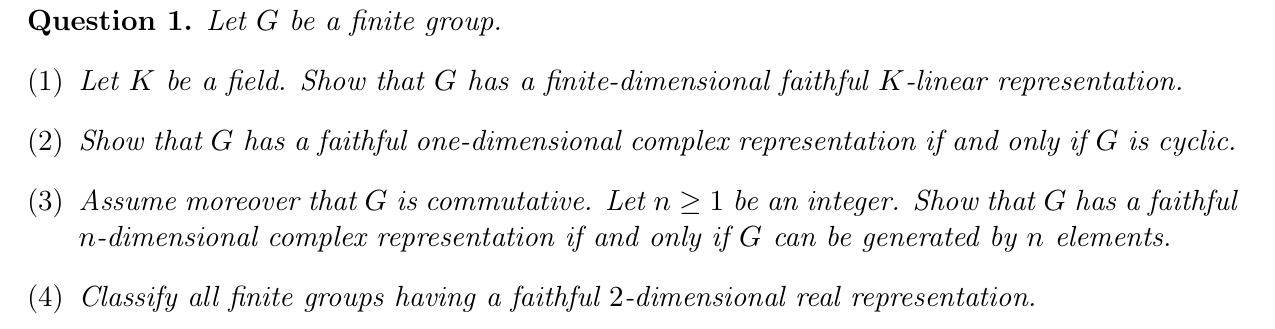
\includegraphics[width=\textwidth]{group-representation-2025050411.png}
% \caption{}
\label{}
\end{figure}
\end{exercise}
(1)
$\lvert G \rvert=n$, $G=\{ g_1,\dots,g_n \}$. Let $V$ be a $K$ -vector space whose basis is $\{ e_{g_1},\dots,e_{g_n} \}$. The dimension of $V$ is $\dim_{K}(V)=\lvert G \rvert$. More formally,
\[
V=\bigoplus_{g\in G}Ke_{g}
\]
$V$ is a finite vector space over $G$. Define the mapping (we will show that it's a representation),
\[
\rho:G\to \mathrm{Hom}(V,V)\qquad g\to \rho_{g}
\]
where $\rho_{g}: e_{h}\mapsto e_{gh}$. We can extend the action linearly to any $v=\sum_{h\in G}^{}\alpha_{h}e_{h}\in V$, by letting
\[
\rho_{g}(v)=\sum_{h\in G}\alpha_{h}e_{gh}
\]
To show that it's a homomorphism, we have
\[
\rho_{gg'}(e_{h})=e_{gg'h}=(\rho_{g}\circ \rho_{g'})(e_{h})\qquad \forall h\in G
\]
To show that the representation is faithful, consider the kernel
\[
\ker \rho=\{ g\in G:\rho(g)=id \}
\]
For $g\in \ker \rho$,
\[
e_{gh}=\rho_{g}(e_{h})=e_{h}\qquad \forall h\in G
\]
Then we have
\[
gh=h\qquad \forall h\in G\implies g=e
\]
Thus $\ker \rho=\{ e \}$. The representation is faithful.

(2)
If $G$ is cyclic with order $n$, and $G= \left< g \right>$, then the mapping
\[
\rho:G\to \mathrm{Hom}(\mathbb{C},\mathbb{C})\qquad g^{r}\mapsto e^{ 2\pi ir/n }
\]
is a faithful representation.

If $G$ has a faithful one-dimensional complex representation,
\[
\rho:G\to \mathrm{Hom}(\mathbb{C},\mathbb{C})\qquad g\mapsto \rho_{g}
\]
$\lvert G \rvert=n$, then $\rho (g)^{n}=1,\forall g\in G$. Thus every $\rho_{g}$ lies in the set of $n^{\text{th}}$ roots of unity, which has size $n$. Since $\rho$ is faithful, $\rho_{g}\neq \rho_{h}$ for $g\neq h$. Then $\rho(G)=\{ \mu _n \}$ is cyclic. Hence $G$ is cyclic.

(3)
If $G$ can be generated by $g_1,\dots,g_n$, then for any $g\in G$, we have
\[
g=g_1^{r_1}\dots g_n^{r_n}
\]
Assume that $g_i^{\alpha _i}=e$ for every $i$, then the mapping
\[
\rho:G\to \mathrm{Hom}(\mathbb{C}^{n},\mathbb{C}^{n})\qquad g\mapsto \mathrm{diag}\{ e^{ 2\pi ir_1/\alpha_1 },\dots e^{ 2\pi i r_n/\alpha _n } \}
\]
is a faithful $n$ -dimensional complex representation.

If $G$ has a faithful $n$ -dimensional complex representation,
\[
\rho:G\to \mathrm{Hom}(\mathbb{C}^{n},\mathbb{C}^{n})\qquad g\mapsto \rho_{g}
\]
$\rho_{g}$ can be a diagonized matrix.
....

(4)
具有忠实的二维实表示的有限群的分类如下:

\begin{enumerate}
	\item 循环群 $C_n$( n 阶循环群),对于任意 $n \geq 1$ 。
	\item 二面体群 $D_m$( 2 m 阶二面体群,即正 m 边形的对称群),对于任意 $m \geq 1$ 。
\end{enumerate}

\begin{remark}
Let $(\rho, V)$ be a finite dimensional $\mathbb{C}$-representation of a finite group $G$. Consider the $G$-invariant subspace
\[
V^G:=\{v \in V \mid \rho(g)(v)=v \text { for all } g \in G\}
\]	\begin{enumerate}
		\item Show that $\operatorname{dim} V^G$ is the same as the multiplicity of the trivial representation appearing in $V$.
		\item Show that $\operatorname{dim} V^G=\frac{1}{|G|} \sum_{g \in G} \chi_\rho(g)$.
		\item Construct a surjective map $\phi: V \rightarrow V^G$, expressed in terms of a linear combination of linear operators $\rho(g)$ for $g \in G$, such that $\phi^2=\phi$ (i.e. $\phi$ is a projection) and $\phi$ is a homomorphism.
	\end{enumerate}
\end{remark}
\begin{figure}[H]
\centering
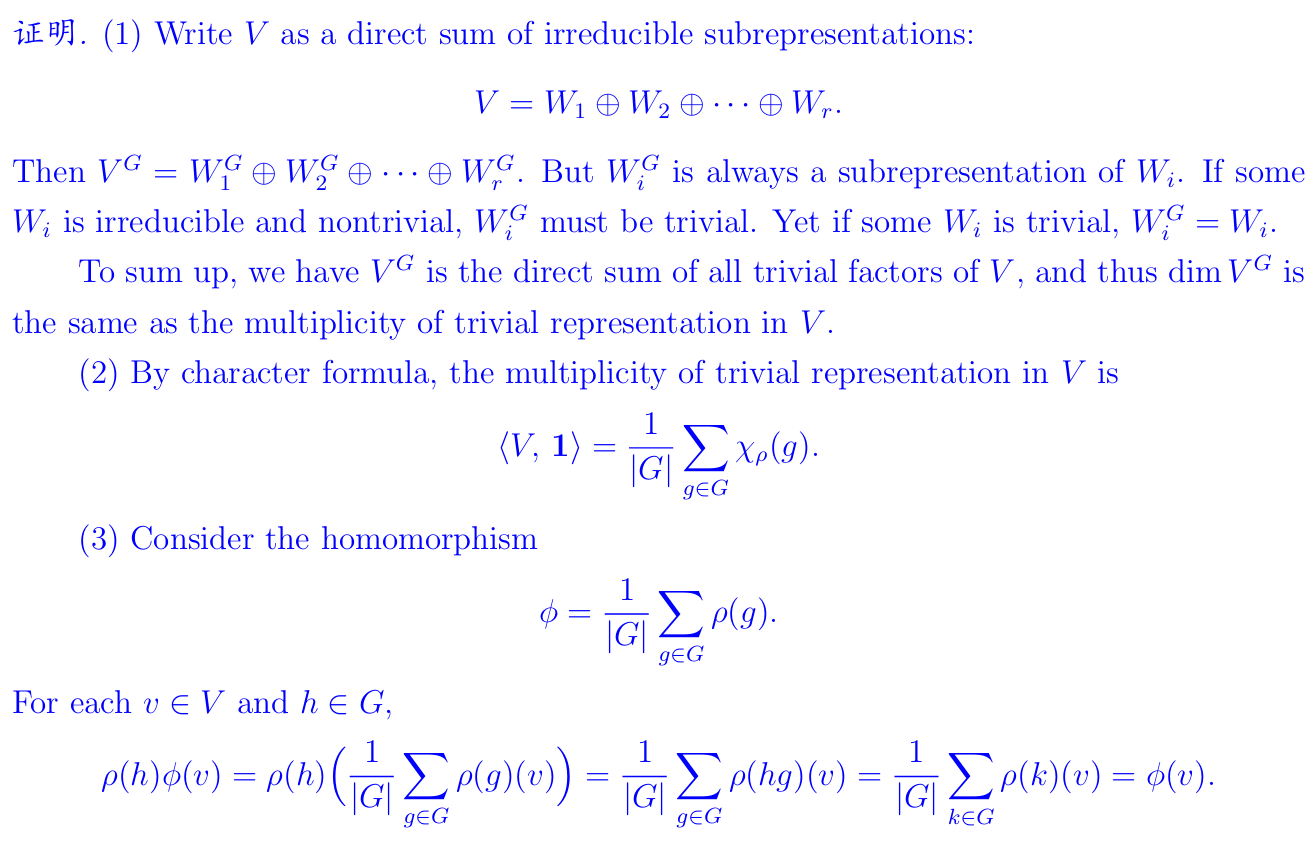
\includegraphics[width=\textwidth]{group-representation-2025051012.png}
% \caption{}
\label{}
\end{figure}
\begin{figure}[H]
\centering
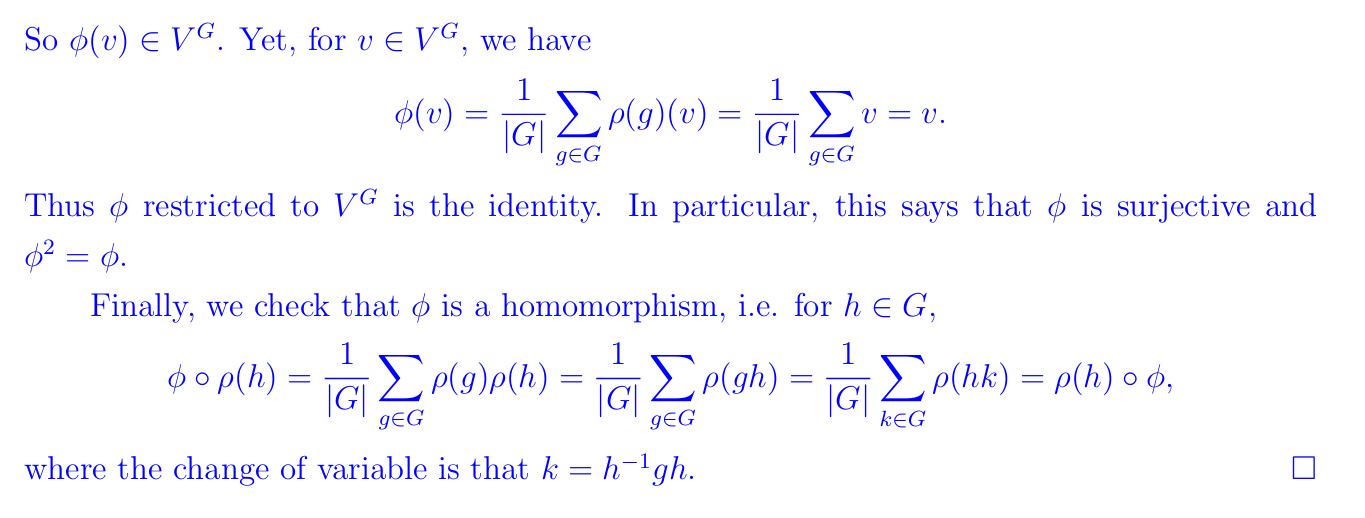
\includegraphics[width=\textwidth]{1-group-representation-2025051012.png}
% \caption{}
\label{}
\end{figure}

\input{表示论/includes/Representation-Theory-and-Character-Theory.tex}
\section{Tensor product}

Let $V$ and $W$ be vector spaces over $\mathbb{C}$ with bases $v_1, \ldots, v_m$ and $w_1, \ldots, w_n$, respectively. For each $i, j$ with $1 \leqslant i \leqslant m, 1 \leqslant j \leqslant n$, we introduce a symbol $v_i \otimes w_j$. The tensor product space $V \otimes W$ is defined to be the mn-dimensional vector space over $\mathbb{C}$ with a basis given by
\[
\left\{v_i \otimes w_j: 1 \leqslant i \leqslant m, 1 \leqslant j \leqslant n\right\}
\]
Thus $V \otimes W$ consists of all expressions of the form
\[
\sum_{i, j} \lambda_{i j}\left(v_i \otimes w_j\right) \quad\left(\lambda_{i j} \in \mathbb{C}\right)
\]
For $\quad v \in V$ and $\quad w \in W$ with $v=\sum_{i=1}^m \lambda_i v_i \quad$ and $\quad w=\sum_{j=1}^n \mu_j w_j$ $\left(\lambda_i, \mu_j \in \mathbb{C}\right)$, we define $v \otimes w \in V \otimes W$ by
\[
v \otimes w=\sum_{i, j} \lambda_i \mu_j\left(v_i \otimes w_j\right) .
\]
For example,
\[
(2v_1-v_2)\otimes (w_1+w_2)=2v_1\otimes w_1+2v_1\otimes w_2-v_2\otimes w_1-v_2\otimes w_2
\]
Do not be misled by the notation into believing that every element of $V\otimes W$ has the form $v\otimes w$, but linear combination of $v_i\otimes w_j$.

If $v\in V, w\in W$ and $\lambda \in \mathbb{C}$, then
\[
v\otimes (\lambda w)=(\lambda v)\otimes w=\lambda(v\otimes w)
\]
If $x_1,\dots, x_{a}\in V$ and $y_1,\dots, y_{b}\in W$, then
\[
\left( \sum_{i=1}^{a} x_i \right)\otimes \left( \sum_{j=1}^{b} y_j \right)=\sum_{i,j}x_i\otimes y_j
\]
Next, we deine the tensor product of two $\mathbb{C}G$ -modules.

Let $G$ be a finite group and let $V$ and $W$ be $\mathbb{C} G$ -modules with bases $v_1, \ldots, v_m$ and $w_1, \ldots, w_n$, respectively. We know that the elements
\[
v_i \otimes w_j \quad(1 \leqslant i \leqslant m, 1 \leqslant j \leqslant n)
\]
give a basis of $V \otimes W$. The multiplication of $v_i \otimes w_j$ by an element of $G$ is defined in the following simple way, which is then extended linearly to a multiplication on the whole of $V \otimes W$.

Let $g\in G$. For all $i$, $j$, define
\[
(v_i\otimes w_j)g=v_ig\otimes w_jg
\]
and, more generally, let
\[
\left( \sum_{i,j}\lambda _{ij} (v_i\otimes w_j)\right)g=\sum_{i,j}\lambda _{ij}(v_ig\otimes w_jg)
\]
for arbitrary complex numbers $\lambda _{ij}$.

\begin{remark}
You should be warned that $(v\otimes w)r\neq vr\otimes wr$ for most elements $r$ in $\mathbb{C}G$, e.g. when $r$ is a scalar multiple of $g$.
\end{remark}
\section{Tensor product of modules}

See dummit\&Foote Sec 10.4

\begin{definition}[$R$-module]
Let $R$ be a ring (associative with 1). An \textbf{$R$-module} (or left $R$-module) is an abelian group $M$ together with an operation $R \times M \to M$, denoted by $(r, m) \mapsto rm$, such that for all $r, s \in R$ and $x, y \in M$:
\[
\begin{aligned}
r(x+y) &= rx + ry \\
(r+s)x &= rx + sx \\
(rs)x &= r(sx) \\
1_R x &= x
\end{aligned}
\]A right $R$-module is defined similarly, with the scalar multiplication on the right $M \times R \to M$, denoted by $(m, r) \mapsto mr$, satisfying analogous axioms.
\end{definition}
Our aim is to "extend" an $R$ -module $N$ to an $S$ -module.

To satisfy the relations necessary for an $S$ -module structure\footnote{$(s_1+s_2) n=s_1 n+s_2 n$, $s(n_1+n_2)=sn_1+sn_2$.} and the compatibility relation with the action of $R$ on $N$ \footnote{$(sr) n=s (rn)$}, we must take the quotient of this abelian group by the subgroup $H$ generated by all elements of the form
\[
\begin{gathered}
\left(s_1+s_2, n\right)-\left(s_1, n\right)-\left(s_2, n\right), \\
\left(s, n_1+n_2\right)-\left(s, n_1\right)-\left(s, n_2\right), \text { and } \\
(s r, n)-(s, r n),
\end{gathered}
\]
The resulting quotient group is denoted by $S\otimes_{R}N$ (or jest $S\otimes N$ if $R$ is clear from the context) and is called the \textbf{tensor product} of $S$ and $N$ over $R$. By the definition of the quotient we have forced the relations
\[
\begin{gathered}
\left(s_1+s_2\right) \otimes n=s_1 \otimes n+s_2 \otimes n, \\
s \otimes\left(n_1+n_2\right)=s \otimes n_1+s \otimes n_2, \text { and } \\
s r \otimes n=s \otimes r n .
\end{gathered}
\]
\begin{definition}[universal property for the tensor product]
\begin{figure}[H]
\centering
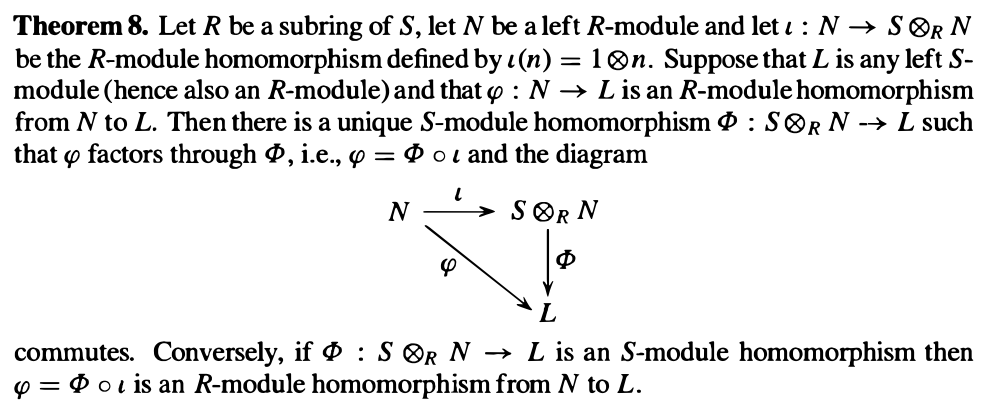
\includegraphics[width=\textwidth]{tensor-product-2025050211.png}
% \caption{}
\label{}
\end{figure}
\end{definition}
\begin{example}
\begin{figure}[H]
\centering
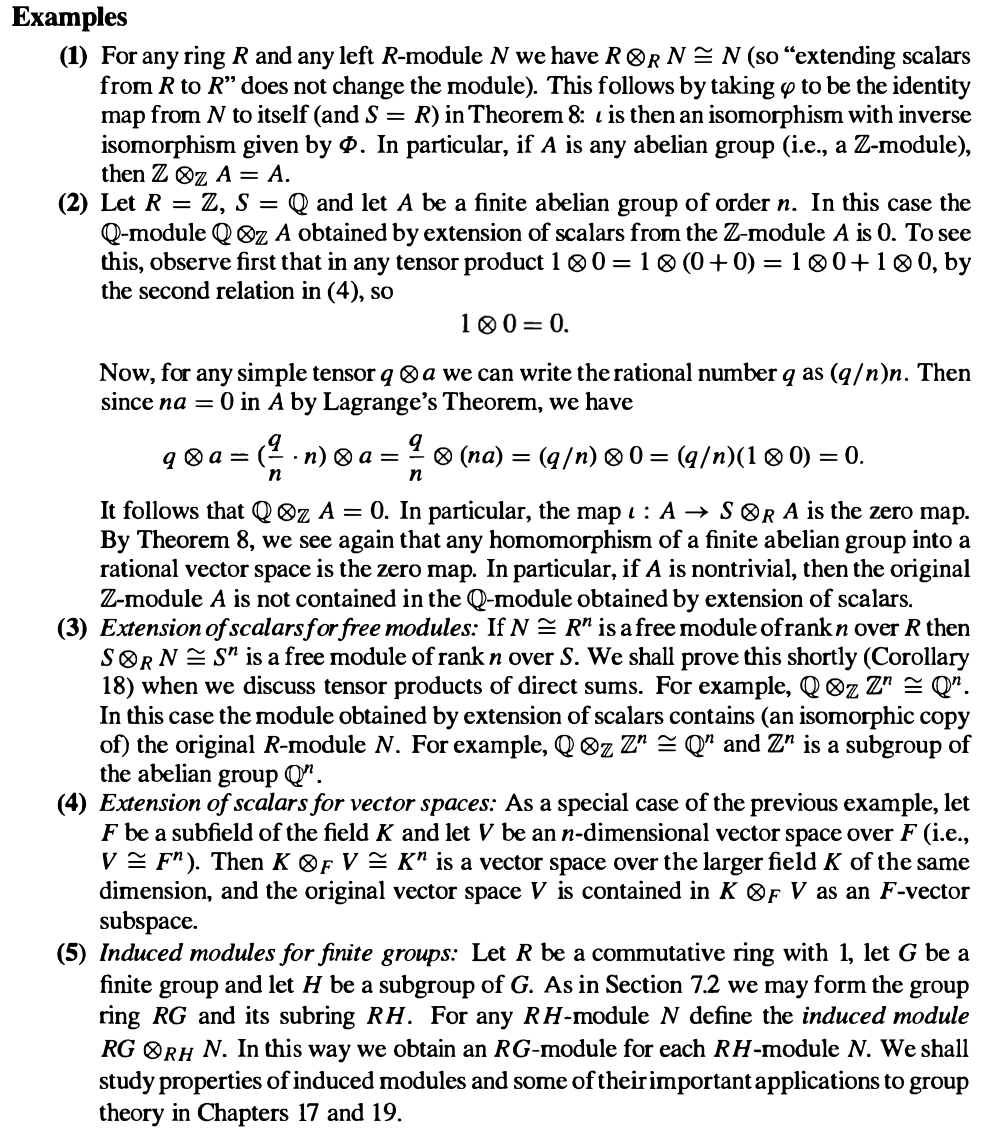
\includegraphics[width=\textwidth]{1-tensor-product-2025050211.png}
% \caption{}
\label{}
\end{figure}
\end{example}
\begin{definition}[$R$ -balanced]
\begin{figure}[H]
\centering
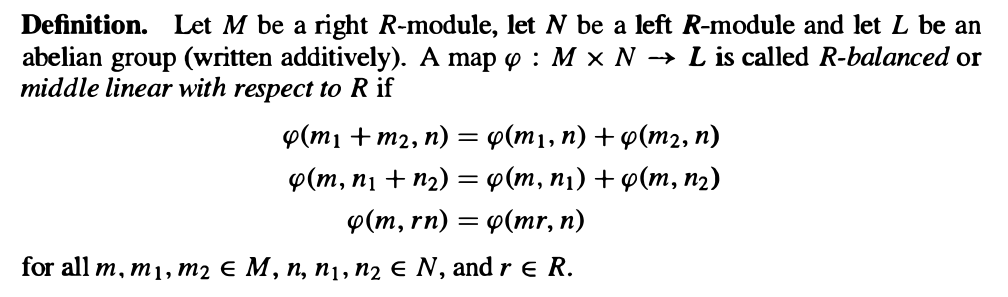
\includegraphics[width=\textwidth]{tensor-product-2025050214.png}
% \caption{}
\label{}
\end{figure}
\end{definition}
\begin{definition}[$R$ -bilinear]
\begin{figure}[H]
\centering
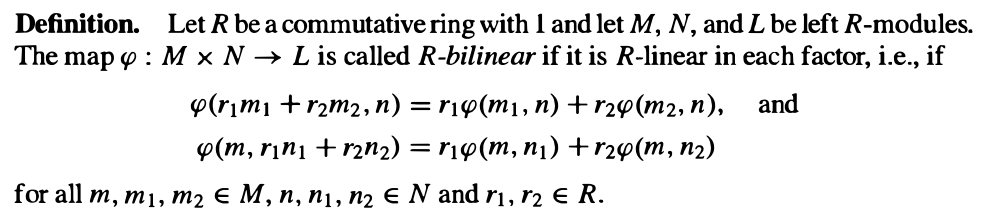
\includegraphics[width=\textwidth]{1-tensor-product-2025050214.png}
% \caption{}
\label{}
\end{figure}
\end{definition}
\begin{example}
We have $\mathbb{Z}_{2}\otimes_{\mathbb{Z}}\mathbb{Z}_{3}=0$, since $3a=a$ for $a\in \mathbb{Z}_{2}$ so that
\[
a\otimes b=3a\otimes b=a\otimes (3b)=a\otimes 0=0
\]
and every simple tensor is reduced to 0. In particular $1\otimes1=0$.
\end{example}
\begin{example}
We have $\mathbb{Z}_{2}\otimes_{\mathbb{Z}}\mathbb{Z}_{2}\cong \mathbb{Z}_{2}$, since $0\otimes0=1\otimes0=0\otimes1=0$ and $1\otimes1$ generates $\mathbb{Z}_{2}\otimes \mathbb{Z}_{2}$.
\end{example}
\begin{example}
$\mathbb{Q}/\mathbb{Z}\otimes_{\mathbb{Z}}\mathbb{Q}/\mathbb{Z}=0$, where a simple tensor has the form $(a/b\ \mathrm{mod}\ \mathbb{Z})\otimes(c/d \ \mathrm{mod}\ \mathbb{Z})$ for some rational numbers $a/b$ and $c/d$. Then
\begin{equation}
\begin{aligned}
\left( \frac{a}{b}\ \mathrm{mod}\ \mathbb{Z} \right)\otimes \left( \frac{c}{d}\ \mathrm{mod}\ \mathbb{Z} \right) & =d\left( \frac{a}{bd}\mod\mathbb{Z} \right)\otimes \left( \frac{c}{d}\mod\mathbb{Z} \right) \\
 & =\left( \frac{a}{bd}\mod\mathbb{Z} \right)\otimes d\left( \frac{c}{d}\mod\mathbb{Z} \right) \\
 & =\left( \frac{a}{bd}\mod\mathbb{Z} \right)\otimes 0 \\
 & =0
\end{aligned}
\label{d2f1db}
\end{equation}
\end{example}

\begin{example}
Similar to \cref{d2f1db}, $A\otimes_{\mathbb{Z}}B=0$ for any divisible abelian group $A$ and \textbf{torsion} abelian group $B$ (an abelian group in which every element has finite order). For exmaple, $\mathbb{Q}\otimes_{\mathbb{Z}}\mathbb{Q}/\mathbb{Z}=0$.
\end{example}
\begin{example}[dimension]
The structure of a tensor product can vary considerably depending on the ring over which the tensors are taken. $\mathbb{Q}\otimes_{\mathbb{Q}}\mathbb{Q}$ and $\mathbb{Q}\otimes_{\mathbb{Z}}\mathbb{Q}$ are isomorphic as left $\mathbb{Q}$ -modules (both are one dimensional vector spaces over $\mathbb{Q}$). Pick any simple tensor $\frac{a}{b}\otimes_{\mathbb{Q}} \frac{c}{d}$ in $\mathbb{Q}\otimes_{\mathbb{Q}}\mathbb{Q}$, then
\[
\frac{a}{b}\otimes \frac{c}{d}=1\otimes \frac{ac}{bd}\to\frac{ac}{bd}
\]
induces an isomorphism between $\mathbb{Q}\otimes_{\mathbb{Q}}\mathbb{Q}$ and $\mathbb{Q}$. Pick any simple tensor $\frac{a}{b}\otimes_{\mathbb{Z}}\frac{c}{d}$ in $\mathbb{Q}\otimes_{\mathbb{Z}}\mathbb{Q}$, then
\[
\frac{a}{b}\otimes \frac{c}{d}=\frac{1}{b}\otimes \frac{ac}{d}=\frac{1}{b}\otimes \left( b\cdot\frac{ac}{bd} \right)=1\otimes \frac{ac}{bd}
\]
Thus $\mathbb{Q}\otimes_{\mathbb{Z}}\mathbb{Q}\cong \mathbb{Q}$. Hence,
\[
\dim _{\mathbb{Q}}(\mathbb{Q}\otimes _{\mathbb{Q}}\mathbb{Q})=\dim _{\mathbb{Q}}(\mathbb{Q}\otimes _{\mathbb{Z}}\mathbb{Q})=1
\]
\end{example}
\begin{example}
On the other hand, $\mathbb{C}\otimes_{\mathbb{C}}\mathbb{C}$ and $\mathbb{C}\otimes_{\mathbb{R}}\mathbb{C}$ are not isomorphic $\mathbb{C}$ -modules (the former is a 1-dimensional vector space over $\mathbb{C}$ and the latter is 2-dimensional over $\mathbb{C}$). Every simple tensor in $\mathbb{C}\otimes_{\mathbb{C}}\mathbb{C}$ has the form $a\otimes b$, then
\[
a\otimes b=1\otimes ab\to ab
\]
induces an isomorphism between $\mathbb{C}\otimes_{\mathbb{C}}\mathbb{C}$ and $\mathbb{C}$. Every simple tensor in $\mathbb{C}\otimes_{\mathbb{R}}\mathbb{C}$ has the form $(a+\mathrm{i}b)\otimes c$, then
\[
(a+\mathrm{i}b)\otimes c=a\otimes c+(\mathrm{i}b)\otimes c=1\otimes (ac)+\mathrm{i}\otimes (bc)\overset{ \simeq  }{ \longrightarrow  }(ac,bc)
\]
induces an isomorphism between $\mathbb{C}\otimes_{\mathbb{R}}\mathbb{C}$ and $\mathbb{C}\oplus \mathbb{C}$. Hence
\[
\dim_{\mathbb{C}} (\mathbb{C}\otimes _{\mathbb{C}}\mathbb{C})=\dim _{\mathbb{C}}\mathbb{C}=1\qquad \dim _{\mathbb{C}}(\mathbb{C}\otimes _{\mathbb{R}}\mathbb{C})=\dim _{\mathbb{C}}(\mathbb{C}\oplus \mathbb{C})=2
\]
\end{example}
\subsection{Dimension}

\href{https://math.stackexchange.com/questions/4306709/dimension-of-a-tensor-product-as-a-vector-space-over-complex-number-field-math}{abstract algebra - Dimension of a tensor product as a vector space over complex number field $\mathbb{C}$ - Mathematics Stack Exchange}

\begin{exercise}
Problem 2 (10 points). Consider the polynomial ring $A=\mathbb{C}[x]$ and its subring $B=\mathbb{C}\left[x^2\right] \subset A$.
Consider $A$ -modules
\[
M=\mathbb{C}[x] /\left(x^2+x\right), \quad N=\mathbb{C}[x] /\left(x^2-1\right)
\]What is the dimension as $\mathbb{C}$ -vector space of each tensor product below? No need to prove or explain.
\end{exercise}
(a) $M \otimes_{\mathbb{C}} N$;

$\mathbb{C}[x]/(x^2+x)\otimes_{\mathbb{C}}\mathbb{C}[x]/(x^2-1)$ has every simple tensor of the form $(a+bx)\otimes_{\mathbb{C}}(c+dx )$, then
\[
\begin{aligned}
(a+bx)\otimes (c+dx ) & =a\otimes c+bx\otimes c+a\otimes dx+bx\otimes dx \\
 & =1\otimes (ac)+x\otimes (bc)+(ad)\otimes x+bd(x\otimes x) \\
 & =ac(1\otimes 1)+bc(x\otimes 1)+ad(1\otimes x)+bd(x\otimes x) \\
 & \to(ac,bc,ad,bd)
\end{aligned}
\]
induces an isomorphism between $\mathbb{C}[x]/(x^2+x)\otimes_{\mathbb{C}}\mathbb{C}[x]/(x^2-1)$ and $\mathbb{C}^{4}$ (the construction is left as an exercise). Therefore
\[
\dim _{\mathbb{C}}(M\otimes _{\mathbb{C}}N)=\dim _{\mathbb{C}}(\mathbb{C}^{4})=4
\]
(b) $M \otimes_A N$;

$\mathbb{C}[x]/(x^2+x)\otimes_{\mathbb{C}[x]}\mathbb{C}[x]/(x^2-1)$ has every simple tensor of the form $(a+bx)\otimes_{\mathbb{C}[x]}(c+dx )$, then
\[
\begin{aligned}
(a+bx)\otimes (c+dx ) & =ac(1\otimes 1)+bc(x\otimes 1)+ad(1\otimes x)+bd(x\otimes x) \\
 & =ac(1\otimes 1)+(bc+ad)((-x^2)\otimes 1)+bd(1\otimes x^2) \\
 & =ac(1\otimes 1)-(bc+ad)(1\otimes x^2)+bd(1\otimes 1) \\
 & =(ac-bc-ad+bd)(1\otimes 1) \\
 & \to ac-bc-ad+bd
\end{aligned}
\]
induces a nature isomorphism between $M\otimes_{A}N$ and $\mathbb{C}$. Therefore,
\[
\dim _{\mathbb{C}}(M\otimes _{A}N)=\dim _{\mathbb{C}}\mathbb{C}=1
\]
(c) $M \otimes_B N$.

$\mathbb{C}[x]/(x^2+x)\otimes_{\mathbb{C}[x^2]}\mathbb{C}[x]/(x^2-1)$ has every simple tensor of the form $(a+bx)\otimes_{\mathbb{C}[x^2]}(c+dx )$, then
\[
\begin{aligned}
(a+bx)\otimes (c+dx  ) & =(a-bx^2)\otimes (c+dx) \\
 & =a\otimes (c+dx )-bx^2\otimes (c+dx) \\
 & =1\otimes (ac+adx)-1\otimes (bcx^2+cdx^3) \\
 & =1\otimes (ac+adx)-1\otimes (bc+cdx) \\
 & =1\otimes [(ac-bc)+(ad-cd)x] \\
 & =(ac-bc)(1\otimes 1)+(ad-cd)(1\otimes x)  \\
 & \to(ac-bc,ad-cd)
\end{aligned}
\]
induces a nature isomorphism between $M\otimes_{B}N$ and $\mathbb{C}^2$. Therefore,
\[
\dim _{\mathbb{C}}(M\otimes _{B}N)=\dim _{\mathbb{C}}(\mathbb{C}^2)=2
\]
We are done!

\section{有限群表示论}

参见肖梁、Artin.

A matrix representation of a group $G$ is a homomorphism
\[
R:G\to \mathrm{GL}_{n}
\]
from $G$ to one of the complex general linear groups. The number $n$ is the dimension of the representation.

We use the notation $R_g$ instead of $R(g)$ for the image of a group element $g$. Each $R_g$ is an invertible matrix, and the statement that $R$ is a homomorphism reads
\[
R_{g h}=R_g R_h .
\]
If a group is given by generators and relations, say $\left\langle x_1, \ldots, x_n \mid r_1, \ldots, r_k\right\rangle$, a matrix representation can be defined by assigning matrices $R_{x_1}, \ldots, R_{x_n}$ that satisfy the relations. For example, the symmetric group $S_3$ can be presented as $\left\langle x, y \mid x^3, y^2, x y x y\right\rangle$, so a representation of $S_3$ is defined by matrices $R_x$ and $R_y$ such that $R_x^3=I, R_y^2=I$, and $R_x R_y R_x R_y=I$. Some relations in addition to these required ones may hold.

\subsection{Defintions of linear represention, homomorphism of representations (\texorpdfstring{$G$}{G} -linear map), isomorphism of representations, subrepresentation, direct sum of representations, complementary representation, irreducible, tensor product, dual representations}

\begin{figure}[H]
\centering
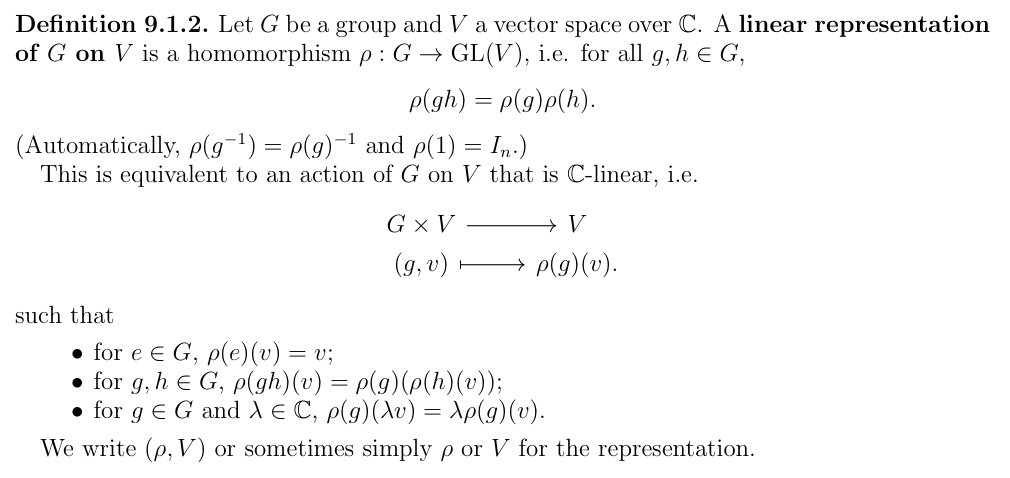
\includegraphics[width=\textwidth]{有限群表示论-2025032521.png}
% \caption{}
\label{}
\end{figure}
\begin{figure}[H]
\centering
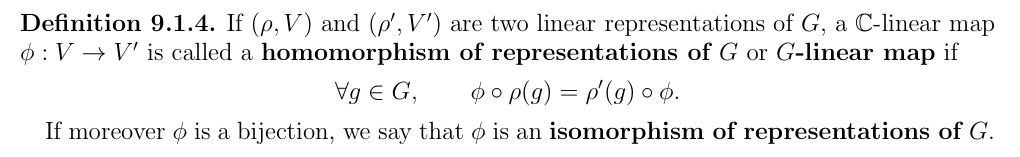
\includegraphics[width=\textwidth]{1-有限群表示论-2025032521.png}
% \caption{}
\label{}
\end{figure}
\begin{figure}[H]
\centering
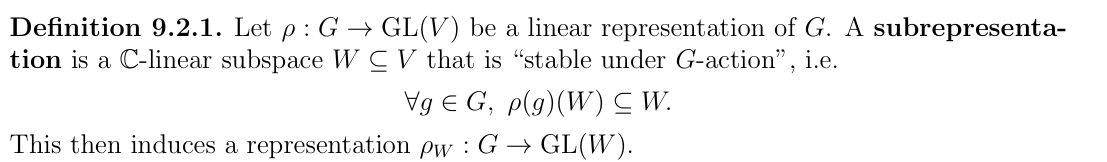
\includegraphics[width=\textwidth]{2-有限群表示论-2025032521.png}
% \caption{}
\label{}
\end{figure}
\begin{figure}[H]
\centering
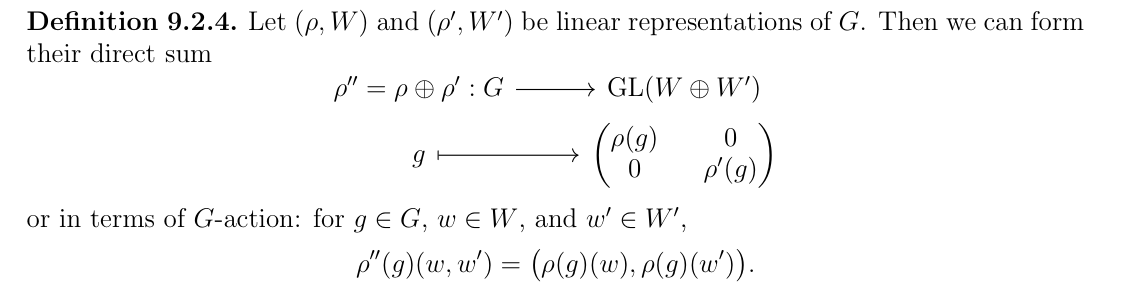
\includegraphics[width=\textwidth]{3-有限群表示论-2025032521.png}
% \caption{}
\label{}
\end{figure}
\begin{figure}[H]
\centering
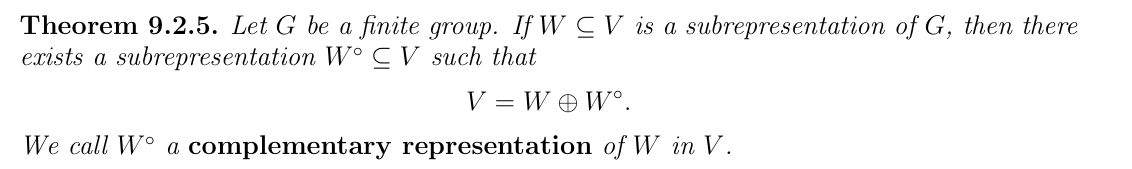
\includegraphics[width=\textwidth]{4-有限群表示论-2025032521.png}
% \caption{}
\label{}
\end{figure}
\begin{figure}[H]
\centering
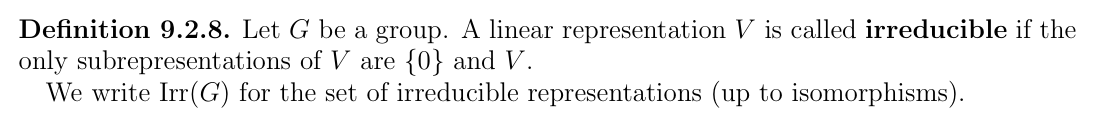
\includegraphics[width=\textwidth]{5-有限群表示论-2025032521.png}
% \caption{}
\label{}
\end{figure}

\begin{note}
If $G$ is finite, then any finite dimensional representation $V$ is "completely reducible".
\begin{figure}[H]
\centering
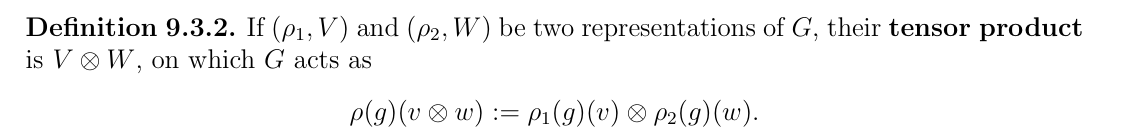
\includegraphics[width=\textwidth]{6-有限群表示论-2025032521.png}
% \caption{}
\label{}
\end{figure}
\begin{figure}[H]
\centering
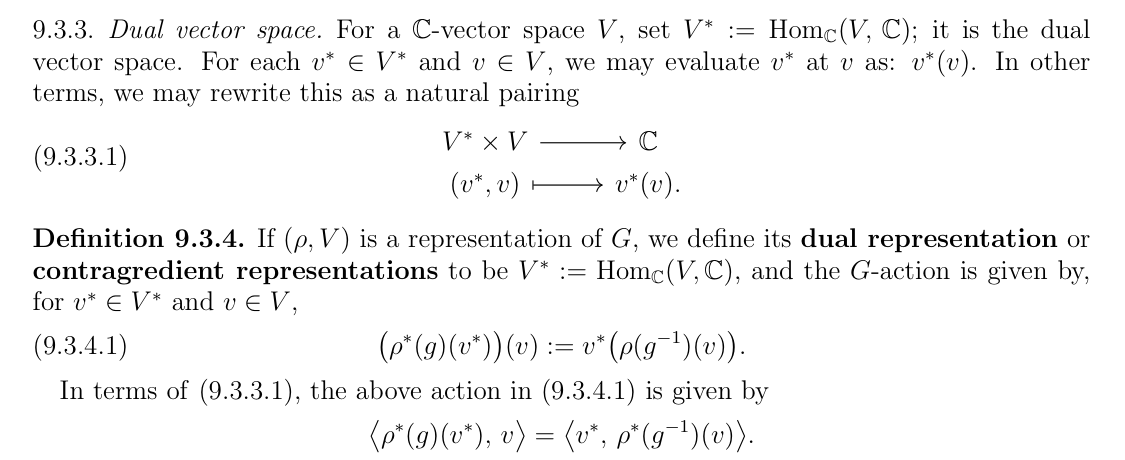
\includegraphics[width=\textwidth]{7-有限群表示论-2025032521.png}
% \caption{}
\label{}
\end{figure}
\begin{figure}[H]
\centering
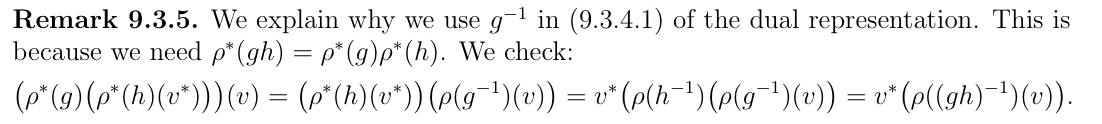
\includegraphics[width=\textwidth]{8-有限群表示论-2025032521.png}
% \caption{}
\label{}
\end{figure}
\begin{figure}[H]
\centering
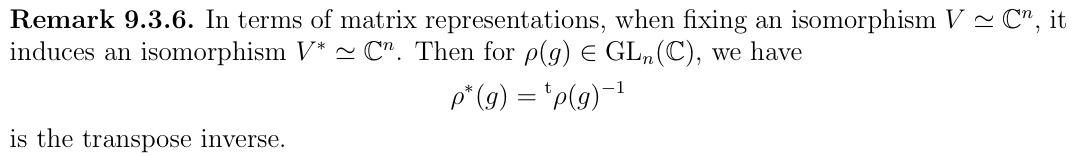
\includegraphics[width=\textwidth]{9-有限群表示论-2025032521.png}
% \caption{}
\label{}
\end{figure}
\end{note}
\subsection{A construction of homomorphism between two linear representations of a finite group \texorpdfstring{$G$}{G}}

\begin{figure}[H]
\centering
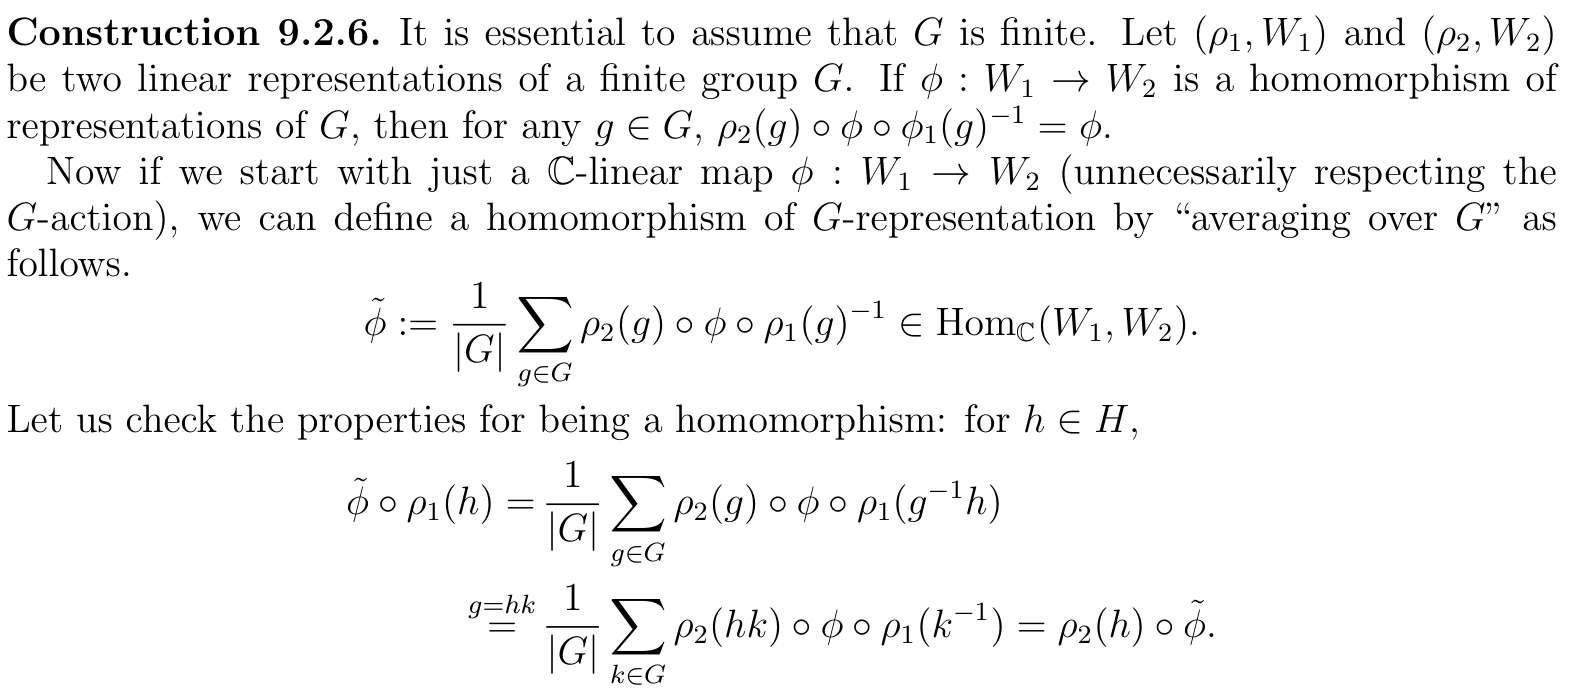
\includegraphics[width=\textwidth]{有限群表示论-2025032601.png}
% \caption{}
\label{}
\end{figure}
\begin{figure}[H]
\centering
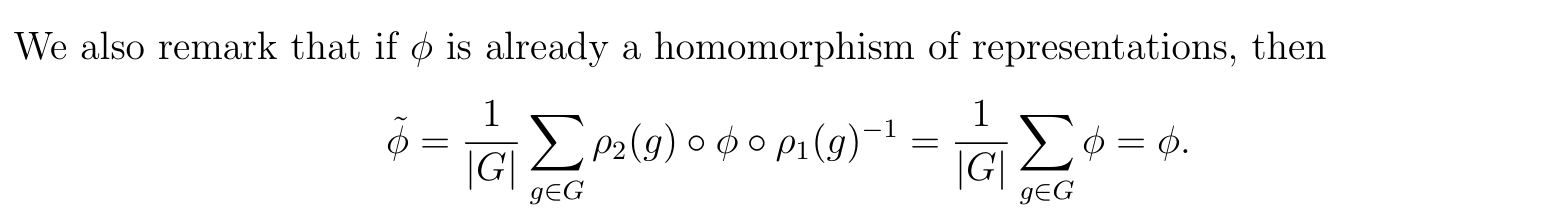
\includegraphics[width=\textwidth]{1-有限群表示论-2025032601.png}
% \caption{}
\label{}
\end{figure}

\subsection{Unitary representations of finite groups}

There is a natural question: can we find a \underline{"good"} matrix representation for a given representation $\rho$ of $G$? Here "good" means there is a positive definite Hermitian form on $V$ so that every $g\in G$ preserves this Hermitian form; and thus the image of $\rho_{\phi}(G)$ in $\mathrm{GL}_{n}(\mathbb{C})$ belongs to the unitary group $\mathrm{U}_n$.

Let $V$ be a Hermitian space -- a complex vector space together with a positive definite Hermitian form $\left< \cdot,\cdot \right>$. A unitary operator $T$ on $V$ is a linear operator with the property
\[
\langle T v, T w\rangle=\langle v, w\rangle\qquad \forall v,w\in V
\]
A representation $\rho:G\to \mathrm{GL}(V)$ on a Hermitian space $V$ is called \textbf{unitary} if $\rho_{g}$ is a unitary operator for every $g$. We can write this condition as
\[
\left< gw,gw \right> = \left< v,w \right> \quad \text{or}\quad \left< \rho_{g}v,\rho_{g}w \right> = \left< v,w \right>
\]
Similarly, a matrix representation $R:G\to \mathrm{GL}_n$ is \textbf{unitary} if $R_{g}\in \mathrm{U}_n,\forall g\in G$. A \textbf{unitary matrix representation} is a homomorphism from $G$ to the unitary group:
\[
R:G\to \mathrm{U}_n
\]
\begin{lemma}
Let $\rho$ be a unitary representation of $G$ on a Hermitian space $V$, and let $W$ be a $G$-invariant subspace. The orthogonal complement $W^{\perp}$ is also $G$-invariant, and $\rho$ is the direct sum of its restrictions to the Hermitian spaces $W$ and $W^{\perp}$. These restrictions are also unitary representations.
\end{lemma}
\begin{proof}
It is true that $V=W \oplus W^{\perp}$. Since $\rho$ is unitary, it preserves orthogonality: If $W$ is invariant and $u \perp W$, then $g u \perp g W=W$. This means that if $u \in W^{\perp}$, then $g u \in W^{\perp}$.
\end{proof}

\subsection{Equivalence of representations}

In matrix terminology, two representation $\varphi$ and $\psi$ are equivalent if there is a fixed invertible matrix $P$ such that
\[
P\varphi(g)P^{-1}=\psi(g)\qquad \forall g\in G
\]
In $FG$ -module terminology, two representation $\varphi$ and $\psi$ are equivalent if there is a fixed $FG$ -module isomorphism $T:V\overset{ \simeq }{ \to }W$ such that
\[
T\circ \varphi(g)=\psi(g)\circ T\qquad \forall g\in G
\]
The linear transformation $T$ or the matrix $P$ above is said to \underline{interwine} the representation $\varphi$ and $\psi$.

\subsection{Characters of representations, class function}

Because they involve several matrices, each of which may have many entries, representations are notationally complicated. The secret to understanding them is to throw out most of the information that the matrices contain, keeping only one essential part, its trace, or character.

Our slogan is: characters determine the representation.
\begin{figure}[H]
\centering
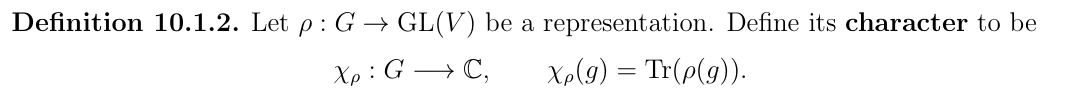
\includegraphics[width=\textwidth]{有限群表示论-2025032522.png}
% \caption{}
\label{}
\end{figure}
\begin{figure}[H]
\centering
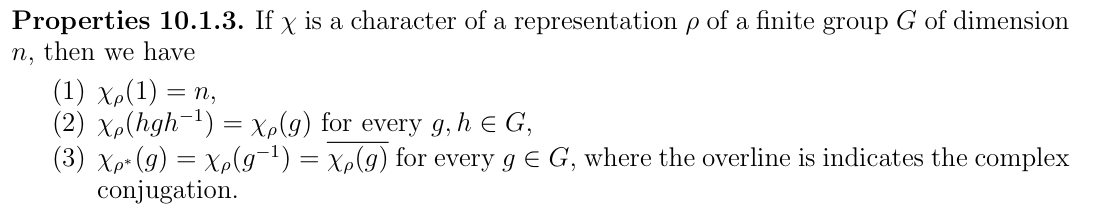
\includegraphics[width=\textwidth]{1-有限群表示论-2025032522.png}
% \caption{}
\label{}
\end{figure}
\begin{figure}[H]
\centering
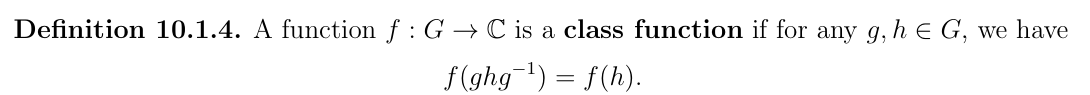
\includegraphics[width=\textwidth]{2-有限群表示论-2025032522.png}
% \caption{}
\label{}
\end{figure}
\begin{figure}[H]
\centering
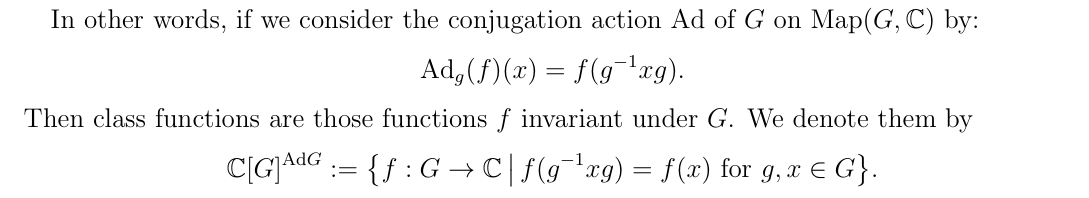
\includegraphics[width=\textwidth]{3-有限群表示论-2025032522.png}
% \caption{}
\label{}
\end{figure}
\begin{figure}[H]
\centering
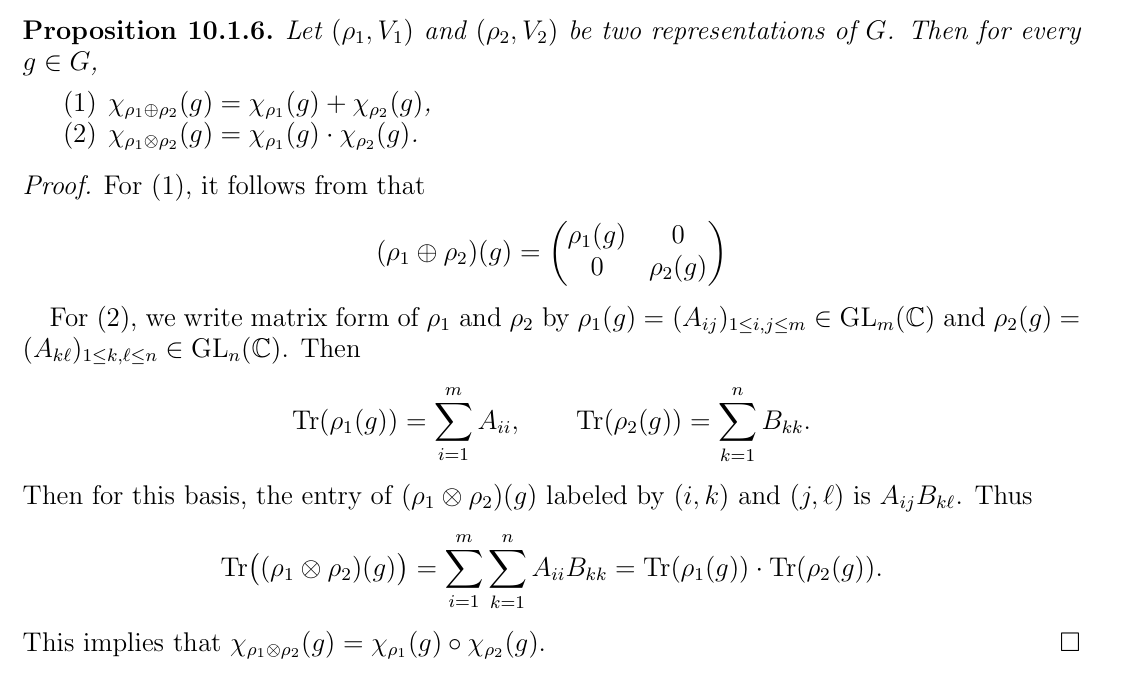
\includegraphics[width=\textwidth]{4-有限群表示论-2025032522.png}
% \caption{}
\label{}
\end{figure}

\subsubsection{Examples}

For $S_3= \left< x,y|x^3,y^3,xyxy \right>$, we have three representaions, $A$, $\Sigma$ and $T$.
\[
A_{x}=\begin{pmatrix}
\cos\frac{2\pi }{3} & -\sin\frac{2\pi}{3} \\
\sin\frac{2\pi}{3} & \cos\frac{2\pi}{3}
\end{pmatrix},\qquad A_{y}=\begin{pmatrix}
1 & 0 \\
0  & -1
\end{pmatrix}
\]
\[
\Sigma_{x}=[1]\qquad \Sigma_{y}=[-1]
\]
\[
T_{x}=[1]\qquad T_{y}=[1]
\]
Then the characters of these representations are displayed below in tabular form.

\begin{table}[h]
	\centering
	\begin{tabular}{|c|c|c|c|c|c|c|}
		\hline
		 & 1 & $x$ & $x^2$ & $y$ & $x y$ & $x^2 y$ \\
		\hline
		$\chi_T$ & 1 & 1 & 1 & 1 & 1 & 1 \\
		\hline
		$\chi_{\Sigma}$ & 1 & 1 & 1 & -1 & -1 & -1 \\
		\hline
		$\chi_A$ & 2 & -1 & -1 & 0 & 0 & 0 \\
		\hline
	\end{tabular}
\end{table}
Several interesting phenomena can be observed in this table:

\begin{itemize}
	\item The rows form orthogonal vectors of length equal to six, which is also the order of $S_3$. The columns are orthogonal too.
	\item $\chi_R(1)$ is the dimension of the representation, also called the dimension of the character.
	\begin{itemize}
		\item Since a representation is a homomorphism, it sends the identity in the group to the identity matrix. So $\chi_R(1)$ is the trace of the identity matrix.
	\end{itemize}
	\item The characters are constant on conjugacy classes.
	\begin{itemize}
		\item The conjugacy classes in $S_3$ are the sets $\{1\},\left\{x, x^2\right\}$, and $\left\{y, x y, x^2 y\right\}$.
		\item This is because conjugate matrices has the same trace.
	\end{itemize}
\end{itemize}

\subsection{Schur's orthogonality}

\begin{figure}[H]
\centering
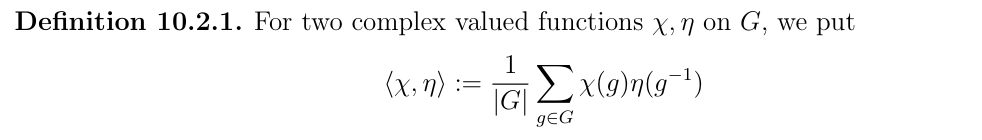
\includegraphics[width=\textwidth]{5-有限群表示论-2025032522.png}
% \caption{}
\label{}
\end{figure}
\begin{figure}[H]
\centering
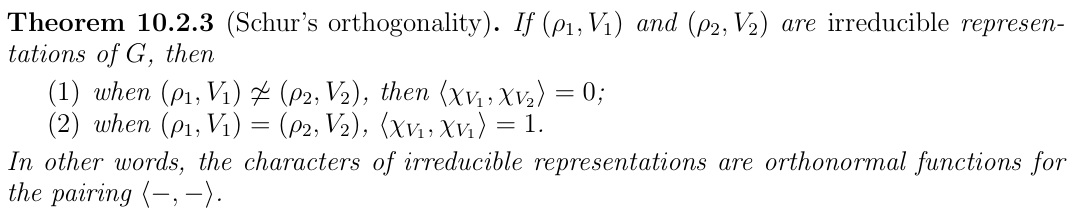
\includegraphics[width=\textwidth]{6-有限群表示论-2025032522.png}
% \caption{}
\label{}
\end{figure}
\begin{figure}[H]
\centering
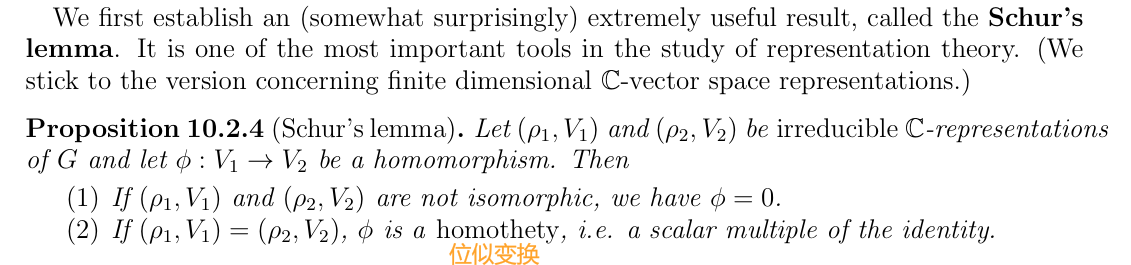
\includegraphics[width=\textwidth]{7-有限群表示论-2025032522.png}
% \caption{}
\label{}
\end{figure}
\begin{figure}[H]
\centering
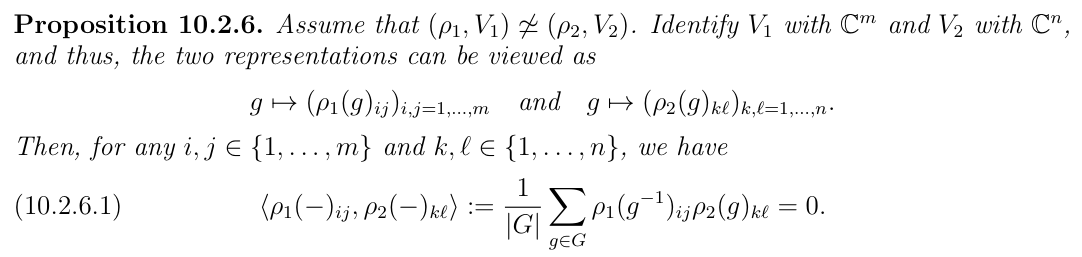
\includegraphics[width=\textwidth]{1-有限群表示论-2025032608.png}
% \caption{}
\label{}
\end{figure}
\begin{figure}[H]
\centering
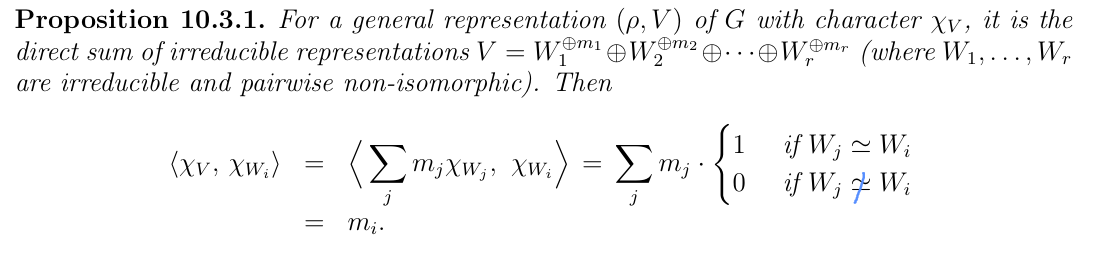
\includegraphics[width=\textwidth]{有限群表示论-2025032608.png}
% \caption{}
\label{}
\end{figure}
\begin{figure}[H]
\centering
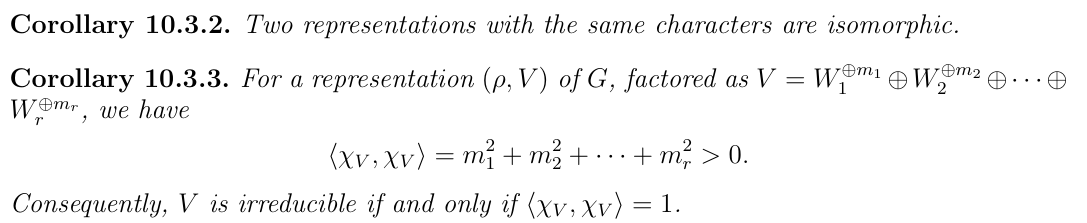
\includegraphics[width=\textwidth]{2-有限群表示论-2025032608.png}
% \caption{}
\label{}
\end{figure}


\chapter{交换代数}
% 交换代数/includes
\section{环和理想}

参见 Atiyah, \href{https://phanpu.github.io/2021/12/26/a-rough-reading-note-for-atiyah-s-commutative-algebra/Commutative_Algebra_Atiyah.pdf}{Commutative\_Algebra\_Atiyah.pdf}

\begin{exercise}
设 $A$ 是环, 令
\[
f = a_{0} + a_{1} x + \cdots + a_{n} x^{n} \in A[x]
\]证明:
	\begin{enumerate}
		\item $f$ 是 $A[x]$ 的可逆元 $\Leftrightarrow a_{0}$ 是 $A$ 中可逆元且 $a_{1}, \cdots, a_{n}$ 是幂零元。
		\item $f$ 幂零 $\Leftrightarrow a_{0}, a_{1}, \cdots, a_{n}$ 幂零。
		\item $f$ 是零因子 $\Leftrightarrow$ 存在着环 $A$ 的非 0 元 $a$ 使得 $a f = 0$。
		\item 如果 $(a_{0}, \cdots, a_{n}) = (1)$, $f$ 就叫本原多项式。证明: 如果 $f, g \in A[x]$, 那么 $f g$ 本原 $\Leftrightarrow f, g$ 均为本原。
	\end{enumerate}
\end{exercise}
\begin{proof}

\begin{enumerate}
	\item $\Leftarrow$: 设 $a_{i}^{m_{i}} = 0, 1 \leq i \leq n$, 不妨 $a_{0} = 1$, 否则考虑 $a_{0}^{-1} f$, 则 $(f-1)^{m_{1}+\cdots+m_{n}} = 0$, 记幂数为 $M$, 从而 $1 = 1-(1-f)^{M} = f((1-f)^{M-1}+\cdots+1)$。(实际上就是题 1)
\end{enumerate}

$\Rightarrow$: 设 $f g = 1$, 且 $g(x) = b_{0}+b_{1} x+\cdots+b_{m} x^{m}$, 令 $x=0$, 可得 $a_{0} b_{0} = 1$, 从而 $a_{0}$ 可逆。

从而有 $\forall k, \sum_{i+j=k} a_{i} b_{j} = 0$(线性代数的结论), 特别的 $a_{n} b_{m} = 0$, $a_{n} b_{m-1} + b_{m} a_{n-1} = 0$, 从而 $a_{n}^{2} b_{m-1} = 0$, 如此往下, $a_{n}^{m+1} b_{0} = 0$, 故 $a_{n}$ 幂零。对其余同理。(由于 $a_n$ 幂零,则 $a_nx^{n}$ 幂零,故 $f-a_nx^{n}=\sum_{i=0}^{n-1}a_ix^{i}\eqqcolon f_1$ 依然可逆,对 $f_1$ 重复上述论证可得 $a_{n-1}$ 幂零,依此类推)
\end{proof}

\section{模与理想}

\begin{proposition}
极大理想都是素理想.
\end{proposition}
\begin{exercise}
$(N:P)=\text{Ann}((P+N)/N)$.
\end{exercise}
\begin{note}
这里使用 $\text{Ann}((P+N)/N)$ 而不是 $\text{Ann}(P/N)$,是因为后者只在 $N\subset P$ 的情况下有定义,而前者总是良好定义的.
\end{note}
\begin{exercise}
\begin{figure}[H]
\centering
\includegraphics[width=\textwidth]{交换代数-2025052111.png}
% \caption{}
\label{}
\end{figure}
\begin{figure}[H]
\centering
\includegraphics[width=\textwidth]{1-交换代数-2025052111.png}
% \caption{}
\label{}
\end{figure}
\end{exercise}
解释 3 的证明:

这个证明的目的是要说明:在一个局部环 $A$ 上,如果两个有限生成的 $A$-模 $M$ 和 $N$ 的张量积 $M \otimes_A N = 0$,那么 $M$ 和 $N$ 中至少有一个是零模。

证明过程可以分解为以下几个步骤:

\subsection{证明步骤详解}

\textbf{引入剩余域 (Residue Field)}

设 $A$ 是一个局部环,其唯一的极大理想为 $\mathfrak{m}$。

考虑 $B = A/\mathfrak{m}$。因为 $\mathfrak{m}$ 是极大理想,所以 $B$ 是一个域,称为 $A$ 的\textbf{剩余域}。

\textbf{张量积与剩余域}

我们已知 $M \otimes_A N = 0$。

将这个等式两边都用 $B = A/\mathfrak{m}$ 在 $A$ 上作张量积,可以得到:
\[
(A/\mathfrak{m}) \otimes_A (M \otimes_A N) = (A/\mathfrak{m}) \otimes_A 0 = 0
\]
利用张量积的结合律和换环定理 (change of rings, $R \otimes_A (M \otimes_A N) \cong (R \otimes_A M) \otimes_R (R \otimes_A N)$,其中 $R$ 是一个 $A$-代数),这里 $R=B=A/\mathfrak{m}$,我们有:
\[
( (A/\mathfrak{m}) \otimes_A M ) \otimes_{A/\mathfrak{m}} ( (A/\mathfrak{m}) \otimes_A N ) = 0
\]
根据题目2的结论 ($A/\mathfrak{a} \otimes_A M \cong M/\mathfrak{a}M$),我们知道:

\begin{itemize}
	\item $B \otimes_A M \cong M/\mathfrak{m}M$。我们记 $M_B = M/\mathfrak{m}M$。
	\item $B \otimes_A N \cong N/\mathfrak{m}N$。我们记 $N_B = N/\mathfrak{m}N$。
\end{itemize}

因此,上面的等式变为 $M_B \otimes_B N_B = 0$。 注意 $M_B$ 和 $N_B$ 都是域 $B$ 上的向量空间。

\textbf{向量空间的张量积}

我们得到了 $M_B \otimes_B N_B = 0$,其中 $M_B$ 和 $N_B$ 是域 $B$ 上的向量空间。

对于域上的向量空间 $V, W$,如果 $V \otimes_B W = 0$,那么必然有 $V=0$ 或者 $W=0$。(如果 $V, W$ 均非零,它们分别有非空基底,则 $V \otimes_B W$ 的基底由它们基底元素的张量积构成,因此 $V \otimes_B W$ 也非零。)

证明中使用了Hom函子的性质来推导这一结论:

\begin{itemize}
	\item 利用张量-Hom伴随 (tensor-hom adjunction):
\[
\text{Hom}_B(M_B \otimes_B N_B, N_B) \cong \text{Hom}_B(M_B, \text{Hom}_B(N_B, N_B))
\]	\item 由于 $M_B \otimes_B N_B = 0$,那么左边的 $\text{Hom}_B(0, N_B)$ 只包含零映射(从零空间到 $N_B$ 的唯一线性映射是零映射)。
	\item 因此,右边的 $\text{Hom}_B(M_B, \text{Hom}_B(N_B, N_B))$ 也必须为零(即只包含零映射)。
	\item 对于域 $B$ 上的向量空间 $X$ 和 $Y$,如果 $\text{Hom}_B(X, Y) = 0$,那么 $X=0$ 或者 $Y=0$。(如果 $X \ne 0$ 且 $Y \ne 0$,我们可以构造一个非零的从 $X$ 到 $Y$ 的线性映射)。
	\item 所以,从 $\text{Hom}_B(M_B, \text{Hom}_B(N_B, N_B)) = 0$ 可以得出:
$M_B = 0$ 或者 $\text{Hom}_B(N_B, N_B) = 0$。
	\item 如果 $\text{Hom}_B(N_B, N_B) = 0$,这意味着从 $N_B$ 到 $N_B$ 的唯一线性映射是零映射。但如果 $N_B \ne 0$,那么其上的恒等映射 $id_{N_B}$ 就不是零映射。所以,$\text{Hom}_B(N_B, N_B) = 0$ 必然意味着 $N_B = 0$。
	\item 综上,我们得出结论:$M_B = 0$ 或者 $N_B = 0$。也就是 $M/\mathfrak{m}M = 0$ 或者 $N/\mathfrak{m}N = 0$。
\end{itemize}

\textbf{应用中山正引理 (Nakayama's Lemma)}

我们已知 $A$ 是一个局部环,$\mathfrak{m}$ 是其唯一的极大理想。$M$ 和 $N$ 是有限生成的 $A$-模。

中山正引理的一个形式是:若 $M$ 是环 $A$ 上的有限生成模,$I$ 是 $A$ 的一个理想且 $I$ 包含于 $A$ 的 Jacobson 根 $J(A)$ 中。如果 $IM=M$,则 $M=0$。

对于局部环 $A$,其 Jacobson 根就是其唯一的极大理想 $\mathfrak{m}$。

所以:

\begin{itemize}
	\item 如果 $M/\mathfrak{m}M = 0$,这意味着 $M = \mathfrak{m}M$。由于 $M$ 是有限生成的 $A$-模,根据中山正引理,可得 $M=0$。
	\item 同理,如果 $N/\mathfrak{m}N = 0$,这意味着 $N = \mathfrak{m}N$。由于 $N$ 是有限生成的 $A$-模,根据中山正引理,可得 $N=0$。
\end{itemize}

\textbf{结论}

因为我们已经证明了 $M/\mathfrak{m}M = 0$ 或者 $N/\mathfrak{m}N = 0$,所以根据中山正引理,必然有 $M=0$ 或者 $N=0$。

这就完成了证明。这个证明巧妙地利用了局部环的性质、剩余域、张量积的性质以及关键的中山正引理。

\begin{exercise}
\begin{figure}[H]
\centering
\includegraphics[width=\textwidth]{2-交换代数-2025052111.png}
% \caption{}
\label{}
\end{figure}
\end{exercise}
证明中指出 "$A[x] = \bigoplus_{i \geq 0} (x^i)$"。这里 $(x^i)$ 指的是由 $x^i$ 生成的 $A$-子模,即 $A \cdot x^i = \{ax^i \mid a \in A\}$。

作为 $A$-模,$A[x]$ 是所有形如 $a_0 + a_1x + a_2x^2 + \cdots + a_nx^n$(其中 $a_j \in A$)的多项式的集合。它可以看作是 $A$-模 $A \cdot 1$,$A \cdot x$,$A \cdot x^2$,… 的直和:
\[
A[x] = A \cdot 1 \oplus A \cdot x \oplus A \cdot x^2 \oplus \cdots = \bigoplus_{i \geq 0} A \cdot x^i.
\]
这意味着 $A[x]$ 是一个自由 $A$ -模,其基为 $\{1, x, x^2, \ldots\}$。


\input{GTM9/includes/Root_Systems_Chapter3_Study_Guide.tex}
\input{GTM9/includes/Root_Systems_Chapter3_Summary_CN.tex}

\chapter{偏微分方程}
% 偏微分方程/includes
\input{偏微分方程/includes/Diffusion.tex}
\input{偏微分方程/includes/Evans-Chap5.tex}
\input{偏微分方程/includes/Fourier分析初步.tex}
\input{偏微分方程/includes/Functional-Analysis.tex}
\section{Fundamental Solution: Laplace equation in \texorpdfstring{$\mathbb{R}^{3}$}{mathbbR^3}}

Okay, let's deduce the fundamental solution of the Laplacian more intuitively. The \textbf{fundamental solution} $\Phi(x)$ is defined as the solution to the equation:
\[
\Delta \Phi(x) = \delta(x)
\]
where $\Delta$ is the Laplacian operator and $\delta(x)$ is the Dirac delta function, representing a point source at the origin. The previous proof concerning the harmonic function $u(x)$ in $\mathbb{R}^3$ used the representation:
\[
u(x) = -\frac{1}{4\pi} \int_{\mathbb{R}^3} \frac{\rho(y)}{|x-y|} dy \quad \text{for} \quad \Delta u = \rho
\]
This implies that the fundamental solution satisfying $\Delta \Phi(x) = \delta(x)$ is $\Phi(x) = -\frac{1}{4\pi|x|}$ in $\mathbb{R}^3$. Let's see how we can arrive at this.

\subsection{1. Intuitive Deduction using Radial Symmetry and Gauss's Law (Divergence Theorem)}

This approach is very physical and geometric, especially for an operator like the Laplacian.

\textbf{a. Radial Symmetry:}

The Dirac delta function $\delta(x)$ is a point source at the origin. It's spherically symmetric (its value depends only on whether $x=0$). We can expect the potential $\Phi(x)$ generated by this point source to also be spherically symmetric. Thus, $\Phi(x)$ should depend only on the distance $r = |x|$ from the origin:
\[
\Phi(x) = \phi(r)
\]
\textbf{b. Laplacian in Spherical Coordinates:}

For a radially symmetric function $\phi(r)$ in $\mathbb{R}^n$, the Laplacian is:
\[
\Delta \phi(r) = \frac{1}{r^{n-1}} \frac{d}{dr} \left( r^{n-1} \frac{d\phi}{dr} \right)
\]
In $\mathbb{R}^3$ (which is the context of the original problem), $n=3$, so:
\[
\Delta \phi(r) = \frac{1}{r^2} \frac{d}{dr} \left( r^2 \frac{d\phi}{dr} \right)
\]
\textbf{c. Solution Away from the Origin ($r > 0$):}

Away from the origin ($x \neq 0$, so $r > 0$), the Dirac delta is zero, $\delta(x) = 0$. So, we must have $\Delta \Phi(x) = 0$.
\[
\frac{1}{r^2} \frac{d}{dr} \left( r^2 \frac{d\phi}{dr} \right) = 0 \quad \text{for } r > 0
\]
This implies that $r^2 \frac{d\phi}{dr}$ must be a constant, let's call it $A$:
\[
r^2 \frac{d\phi}{dr} = A
\]
So,
\[
\frac{d\phi}{dr} = \frac{A}{r^2}
\]
Integrating with respect to $r$ gives:
\[
\phi(r) = -\frac{A}{r} + B
\]
where $B$ is another constant. For potentials that vanish at infinity (which is a common physical condition, and matches $u(x) \to 0$ in the problem), we typically set $B=0$. So, $\phi(r) = -A/r$.

\textbf{d. Determining the Constant A (using the source):}

To find $A$, we use the defining equation $\Delta \Phi(x) = \delta(x)$. Integrate both sides over a small ball $B(0, \epsilon)$ of radius $\epsilon$ centered at the origin:
\[
\int_{B(0,\epsilon)} \Delta \Phi(x) dV = \int_{B(0,\epsilon)} \delta(x) dV
\]
The right side, by definition of the Dirac delta, is $1$.
For the left side, we use the Divergence Theorem (Gauss's Law):
\[
\int_{B(0,\epsilon)} \Delta \Phi(x) dV = \int_{\partial B(0,\epsilon)} \nabla \Phi(x) \cdot \mathbf{n} dS
\]
where $\partial B(0,\epsilon)$ is the sphere of radius $\epsilon$, and $\mathbf{n}$ is the outward unit normal vector.
Since $\Phi(x) = \phi(r)$, its gradient is $\nabla \Phi(x) = \frac{d\phi}{dr} \frac{x}{|x|} = \frac{d\phi}{dr} \mathbf{e}_r$, where $\mathbf{e}_r$ is the radial unit vector. The outward normal $\mathbf{n}$ on the sphere is also $\mathbf{e}_r$.
So, $\nabla \Phi(x) \cdot \mathbf{n} = \frac{d\phi}{dr}$. At $r=\epsilon$, this is $\left.\frac{d\phi}{dr}\right|_{r=\epsilon} = \frac{A}{\epsilon^2}$.
The surface area of the sphere $\partial B(0,\epsilon)$ in $\mathbb{R}^3$ is $4\pi\epsilon^2$.
So the surface integral becomes:
\[
\int_{\partial B(0,\epsilon)} \frac{A}{\epsilon^2} dS = \frac{A}{\epsilon^2} (4\pi\epsilon^2) = 4\pi A
\]
Equating this to the integral of the Dirac delta:
\[
4\pi A = 1 \implies A = \frac{1}{4\pi}
\]
Substituting this back into $\phi(r) = -A/r$:
\[
\phi(r) = -\frac{1}{4\pi r}
\]
Thus, the fundamental solution in $\mathbb{R}^3$ is:
\[
\Phi(x) = -\frac{1}{4\pi|x|}
\]
This is precisely the kernel that appeared in the integral representation for $u(x)$ in the problem you referenced.

\textbf{Intuition from Flux Spreading:}

Imagine a "flux" emanating from the point source at the origin.

\begin{itemize}
	\item The term $r^{n-1} \frac{d\phi}{dr}$ (which is $r^2 \frac{d\phi}{dr}$ in $\mathbb{R}^3$) can be thought of as proportional to the total flux of $\nabla \phi$ through a sphere of radius $r$.
	\item The condition $\Delta \phi = 0$ for $r>0$ means this flux is constant for any $r>0$.
	\item The strength of the field (gradient) $\frac{d\phi}{dr}$ must therefore decrease as $1/r^{n-1}$ to keep the flux constant, because the surface area of the sphere is proportional to $r^{n-1}$.
	\begin{itemize}
		\item In $\mathbb{R}^3$, surface area $\sim r^2$, so field $\sim 1/r^2$. Potential $\phi(r) \sim 1/r$.
		\item In $\mathbb{R}^2$, surface area (circumference) $\sim r$, so field $\sim 1/r$. Potential $\phi(r) \sim \ln r$.
	\end{itemize}
	\item The constant value of this flux is determined by the strength of the source $\delta(x)$, which is $1$ when integrated. This directly gives the constant $A$.
\end{itemize}

\subsection{2. Deduction using Fourier Transform}

This method is more algebraic and general for constant-coefficient linear PDEs.

Let $\widehat{f}(k) = \mathcal{F}\{f(x)\}(k) = \int_{\mathbb{R}^n} f(x) e^{-i k \cdot x} dx$ be the Fourier transform.
The equation is $\Delta \Phi(x) = \delta(x)$.
Taking the Fourier transform of both sides:
\[
\mathcal{F}\{\Delta \Phi(x)\}(k) = \mathcal{F}\{\delta(x)\}(k)
\]
\begin{itemize}
	\item \textbf{FT of Dirac Delta:} $\mathcal{F}\{\delta(x)\}(k) = 1$.
	\item \textbf{FT of Laplacian:} The Fourier transform of $\frac{\partial^2}{\partial x_j^2} \Phi(x)$ is $(i k_j)^2 \widehat{\Phi}(k) = -k_j^2 \widehat{\Phi}(k)$.
So, $\mathcal{F}\{\Delta \Phi(x)\}(k) = \mathcal{F}\left\{\sum_{j=1}^n \frac{\partial^2 \Phi}{\partial x_j^2}\right\}(k) = \sum_{j=1}^n (-k_j^2) \widehat{\Phi}(k) = -|k|^2 \widehat{\Phi}(k)$.
\end{itemize}

Putting these together, the equation in Fourier space becomes:
\[
-|k|^2 \widehat{\Phi}(k) = 1
\]
So, the Fourier transform of the fundamental solution is:
\[
\widehat{\Phi}(k) = -\frac{1}{|k|^2}
\]
Now, we need to find the inverse Fourier transform $\Phi(x) = \mathcal{F}^{-1}\{-\frac{1}{|k|^2}\}(x)$:
\[
\Phi(x) = -\int_{\mathbb{R}^n} \frac{1}{|k|^2} e^{i k \cdot x} \frac{dk}{(2\pi)^n}
\]
This integral needs to be computed.

\textbf{For $n=3$ (as in the problem):}
\[
\Phi(x) = -\frac{1}{(2\pi)^3} \int_{\mathbb{R}^3} \frac{1}{|k|^2} e^{i k \cdot x} dk
\]
To evaluate this, we can use spherical coordinates for $k=(k_1, k_2, k_3)$. Let $s = |k|$. By rotating coordinates, we can align $x$ with the $z$-axis, so $x=(0,0,|x|)$, and $k \cdot x = s |x| \cos\psi$, where $\psi$ is the angle between $k$ and $x$. The volume element is $dk = s^2 \sin\psi ds d\psi d\theta_k$ (where $\theta_k$ is the azimuthal angle for $k$).
\[
\begin{aligned}
\Phi(x) &= -\frac{1}{(2\pi)^3} \int_0^\infty \int_0^\pi \int_0^{2\pi} \frac{1}{s^2} e^{i s |x| \cos\psi} s^2 \sin\psi d\theta_k d\psi ds \\
&= -\frac{2\pi}{(2\pi)^3} \int_0^\infty \left( \int_0^\pi e^{i s |x| \cos\psi} \sin\psi d\psi \right) ds
\end{aligned}
\]
The inner integral is
\[
\int_0^\pi e^{i s |x| \cos\psi} \sin\psi d\psi = \left[ -\frac{e^{i s |x| \cos\psi}}{i s |x|} \right]_0^\pi = -\frac{e^{-i s |x|} - e^{i s |x|}}{i s |x|} = \frac{2\sin(s|x|)}{s|x|}
\]
So,
\[
\begin{aligned}
\Phi(x) &= -\frac{1}{4\pi^2} \int_0^\infty \frac{2\sin(s|x|)}{s|x|} ds \\
&= -\frac{1}{2\pi^2 |x|} \int_0^\infty \frac{\sin(s|x|)}{s} ds
\end{aligned}
\]
Let $t = s|x|$, then $ds = dt/|x|$. The integral becomes
\[
\int_0^\infty \frac{\sin t}{t/|x|} \frac{dt}{|x|} = \int_0^\infty \frac{\sin t}{t} dt
\]
This is the Dirichlet integral, which evaluates to $\pi/2$.
\[
\Phi(x) = -\frac{1}{2\pi^2 |x|} \cdot \frac{\pi}{2} = -\frac{1}{4\pi|x|}
\]
This matches the result from the radial symmetry method.

\textbf{Intuition from Fourier Transform:}

\begin{itemize}
	\item The Laplacian $\Delta$ acts as a multiplication by $-|k|^2$ in Fourier space. It heavily attenuates high frequencies.
	\item The Dirac delta $\delta(x)$ has a flat spectrum (all frequencies equally present: $\widehat{\delta}(k)=1$).
	\item $\widehat{\Phi}(k) = -1/|k|^2$ means the fundamental solution has a spectrum that decays fairly slowly for small $|k|$ (it's singular at $k=0$) and faster for large $|k|$. This $1/|k|^2$ behavior in Fourier space is characteristic of $1/|x|$ type potentials in real space for 3D. The singularity at $k=0$ in $\widehat{\Phi}(k)$ hints at the long-range nature of the potential $\Phi(x)$.
\end{itemize}

Both methods yield the same result. The radial symmetry/Gauss's law approach is often more physically intuitive for the Laplacian, while the Fourier transform method is a very powerful and general algebraic tool applicable to a wider range of constant-coefficient linear differential operators.

\section{Fundamental Solution: Laplace, heat, wave equation in \texorpdfstring{$\mathbb{R}^{n}$}{mathbbR^n}}

\subsection{1. Laplace Equation}

The fundamental solution $G(x)$ for the Laplace equation satisfies
\[
\Delta_x G(x)=\delta(x) \quad \text { in } \mathbb{R}^n
\]
where $\Delta_x=\sum_{j=1}^n \frac{\partial^2}{\partial x_j^2}$ is the Laplacian operator.

\begin{enumerate}
	\item \textbf{Fourier Transform:}
\end{enumerate}

Applying the Fourier transform with respect to $x$ to both sides:
\[
\mathcal{F}_x\{\Delta_x G(x)\}(k)=\mathcal{F}_x\{\delta(x)\}(k)
\]
We know that $\mathcal{F}_x\{\delta(x)\}(k)=1$. For the left side, the derivative property of Fourier transforms gives $\mathcal{F}_x\{\frac{\partial}{\partial x_j} f(x)\}(k)=i k_j \widehat{f}(k)$. Thus, $\mathcal{F}_x\{\frac{\partial^2}{\partial x_j^2} f(x)\}(k)=\left(i k_j\right)^2 \widehat{f}(k)=-k_j^2 \widehat{f}(k)$.
So, $\mathcal{F}_x\{\Delta_x G(x)\}(k)=\sum_{j=1}^n\left(-k_j^2\right) \widehat{G}(k)=-|k|^2 \widehat{G}(k)$.
The transformed equation is:
\[
-|k|^2 \widehat{G}(k)=1
\]
Solving for $\widehat{G}(k)$:
\[
\widehat{G}(k)=-\frac{1}{|k|^2}
\]
\begin{enumerate}
	\item \textbf{Inverse Fourier Transform:}
\end{enumerate}

Now we need to compute the inverse Fourier transform:
\[
G(x)=-\frac{1}{(2 \pi)^n} \int_{\mathbb{R}^n} \frac{1}{|k|^2} e^{i k \cdot x} d^n k
\]
\begin{itemize}
	\item \textbf{Case $n>2$:}
\end{itemize}

We use the Schwinger parametrization $\frac{1}{A}=\int_0^\infty e^{-s A} d s$. Here $A=|k|^2$:
\[
\frac{1}{|k|^2}=\int_0^\infty e^{-s|k|^2} d s
\]
Substituting this into the integral for $G(x)$:
\[
G(x)=-\frac{1}{(2 \pi)^n} \int_{\mathbb{R}^n}\left(\int_0^\infty e^{-s|k|^2} d s\right) e^{i k \cdot x} d^n k
\]
Assuming we can interchange the order of integration:
\[
G(x)=-\frac{1}{(2 \pi)^n} \int_0^\infty\left(\int_{\mathbb{R}^n} e^{-s|k|^2+i k \cdot x} d^n k\right) d s
\]
The inner integral is an $n$-dimensional Gaussian integral. The exponent is $-s|k|^2+i k \cdot x=-s \sum_j k_j^2+i \sum_j k_j x_j$.
Completing the square for each component $k_j$ : $-s k_j^2+i k_j x_j=-s\left(k_j-\frac{i x_j}{2 s}\right)^2-\frac{x_j^2}{4 s}$.
\[
\int_{\mathbb{R}^n} e^{-s|k|^2+i k \cdot x} d^n k=\prod_{j=1}^n \int_{-\infty}^\infty e^{-s\left(k_j-\frac{i x_j}{2 s}\right)^2-\frac{x_j^2}{4 s}} d k_j=e^{-\frac{|x|^2}{4 s}} \prod_{j=1}^n \int_{-\infty}^\infty e^{-s K_j^2} d K_j
\]
Since $\int_{-\infty}^\infty e^{-s K^2} d K=\sqrt{\frac{\pi}{s}}$, the $n$-dimensional integral is $e^{-\frac{|x|^2}{4 s}}\left(\frac{\pi}{s}\right)^{n / 2}$.
Substituting this back:
\[
G(x)=-\frac{1}{(2 \pi)^n}(\pi)^{n / 2} \int_0^\infty s^{-n / 2} e^{-\frac{|x|^2}{4 s}} d s=-\frac{1}{2^n \pi^{n / 2}} \int_0^\infty s^{-n / 2} e^{-\frac{|x|^2}{4 s}} d s
\]
Let $t=\frac{|x|^2}{4 s}$. Then $s=\frac{|x|^2}{4 t}$, so $d s=-\frac{|x|^2}{4 t^2} d t$.
The integral becomes (for $n>2$, so $n / 2-1>0$ for convergence of $\Gamma(n / 2-1)$ ):
\[
\int_0^\infty s^{-n / 2} e^{-\frac{|x|^2}{4 s}} d s=\int_\infty^0\left(\frac{4 t}{|x|^2}\right)^{n / 2} e^{-t}\left(-\frac{|x|^2}{4 t^2}\right) d t=\frac{2^{n-2}}{|x|^{n-2}} \int_0^\infty t^{n / 2-2} e^{-t} d t=\frac{2^{n-2}}{|x|^{n-2}} \Gamma(n / 2-1)
\]
So, for $n>2$ :
\[
G(x)=-\frac{1}{2^n \pi^{n / 2}} \frac{2^{n-2}}{|x|^{n-2}} \Gamma(n / 2-1)=-\frac{\Gamma(n / 2-1)}{4 \pi^{n / 2}|x|^{n-2}}
\]
For example, if $n=3$, $G(x)=-\frac{\Gamma(1 / 2)}{4 \pi^{3 / 2}|x|}=-\frac{\sqrt{\pi}}{4 \pi \sqrt{\pi}|x|}=-\frac{1}{4 \pi|x|}$.

\begin{itemize}
	\item \textbf{Case $n=2$:}
\end{itemize}

The above derivation for the $s$-integral requires $n / 2-1>0$, so it doesn't directly apply to $n=2$. The direct Fourier inversion of $-1 /|k|^2$ in 2D is subtle. The known result is:
\[
G(x)=\frac{1}{2 \pi} \ln |x|
\]
This can be verified by showing $\Delta G(x)=\delta(x)$ in the distributional sense.

\begin{itemize}
	\item \textbf{Case $n=1$:}
\end{itemize}

Similarly, for $n=1, \widehat{G}(k)=-1 / k^2$. Direct inversion is subtle. The known result is:
\[
G(x)=\frac{1}{2}|x|
\]
This satisfies $\frac{d^2}{d x^2} G(x)=\delta(x)$.


\subsection{2. Heat Equation}

The fundamental solution (or heat kernel) $G(x, t)$ satisfies the homogeneous heat equation with a Dirac delta initial condition:
\[
\left(\partial_t-\alpha \Delta_x\right) G(x, t)=0 \quad \text { for } t>0, x \in \mathbb{R}^n
\]
\[
G(x, 0)=\delta(x)
\]
where $\alpha>0$ is the thermal diffusivity.

\begin{enumerate}
	\item \textbf{Spatial Fourier Transform:}
\end{enumerate}

Let $\widehat{G}(k, t)=\mathcal{F}_x\{G(x, t)\}(k)$. Applying the Fourier transform to the PDE:
\[
\partial_t \widehat{G}(k, t)-\alpha\left(-|k|^2\right) \widehat{G}(k, t)=0
\]
\[
\partial_t \widehat{G}(k, t)=-\alpha|k|^2 \widehat{G}(k, t)
\]
The initial condition transforms to $\widehat{G}(k, 0)=\mathcal{F}_x\{\delta(x)\}(k)=1$.

\begin{enumerate}
	\item \textbf{Solve the ODE in Time:}
\end{enumerate}

This is a first-order ODE for $\widehat{G}(k, t)$ with respect to $t$:
\[
\widehat{G}(k, t)=C(k) e^{-\alpha|k|^2 t}
\]
Using the initial condition $\widehat{G}(k, 0)=1$, we find $C(k)=1$. So, for $t>0$ :
\[
\widehat{G}(k, t)=e^{-\alpha|k|^2 t}
\]
\begin{enumerate}
	\item \textbf{Inverse Spatial Fourier Transform:}
\end{enumerate}
\[
G(x, t)=\mathcal{F}_k^{-1}\left\{e^{-\alpha|k|^2 t}\right\}(x)=\frac{1}{(2 \pi)^n} \int_{\mathbb{R}^n} e^{-\alpha|k|^2 t} e^{i k \cdot x} d^n k
\]
The exponent is $-\alpha t|k|^2+i k \cdot x=-\alpha t \sum_j k_j^2+i \sum_j k_j x_j$.
We complete the square for each component $k_j$ :
\[
-\alpha t k_j^2+i k_j x_j=-\alpha t\left(k_j^2-\frac{i x_j}{\alpha t} k_j\right)=-\alpha t\left(\left(k_j-\frac{i x_j}{2 \alpha t}\right)^2+\frac{x_j^2}{4 \alpha^2 t^2}\right)=-\alpha t\left(k_j-\frac{i x_j}{2 \alpha t}\right)^2-\frac{x_j^2}{4 \alpha t}
\]
The integral becomes:
\[
G(x, t)=\frac{1}{(2 \pi)^n} e^{-\frac{|x|^2}{4 \alpha t}} \prod_{j=1}^n \int_{-\infty}^\infty e^{-\alpha t\left(k_j-\frac{i x_j}{2 \alpha t}\right)^2} d k_j
\]
Each 1D Gaussian integral is $\int_{-\infty}^\infty e^{-\alpha t K_j^2} d K_j=\sqrt{\frac{\pi}{\alpha t}}$.
Therefore:
\[
G(x, t)=\frac{1}{(2 \pi)^n} e^{-\frac{|x|^2}{4 \alpha t}}\left(\frac{\pi}{\alpha t}\right)^{n / 2}=\frac{\pi^{n / 2}}{(2 \pi)^n(\alpha t)^{n / 2}} e^{-\frac{|x|^2}{4 \alpha t}}
\]
\[
G(x, t)=\frac{1}{(4 \pi \alpha t)^{n / 2}} e^{-\frac{|x|^2}{4 \alpha t}} \quad \text { for } t>0
\]

\subsection{3. Wave Equation}

The fundamental solution $G(x, t)$ for the wave equation satisfies:
\[
\left(\partial_t^2-c^2 \Delta_x\right) G(x, t)=\delta(x) \delta(t) \quad \text { in } \mathbb{R}^n \times \mathbb{R}
\]
where $c>0$ is the wave speed. We seek the retarded Green's function, satisfying $G(x, t)=0$ for $t<0$.

\begin{enumerate}
	\item \textbf{Space-Time Fourier Transform:}
\end{enumerate}

Let $\widetilde{G}(k, \omega)=\mathcal{F}_{x, t}\{G(x, t)\}(k, \omega)$.
\[
\mathcal{F}\left\{\partial_t^2 G\right\}=(i \omega)^2 \widetilde{G}(k, \omega)=-\omega^2 \widetilde{G}(k, \omega).
\]
\[
\mathcal{F}\left\{-c^2 \Delta_x G\right\}=-c^2\left(-|k|^2\right) \widetilde{G}(k, \omega)=c^2|k|^2 \widetilde{G}(k, \omega).
\]
\[
\mathcal{F}\{\delta(x) \delta(t)\}=1.
\]
The transformed equation is:
\[
\left(-\omega^2+c^2|k|^2\right) \widetilde{G}(k, \omega)=1
\]
\[
\widetilde{G}(k, \omega)=\frac{1}{c^2|k|^2-\omega^2}
\]
\begin{enumerate}
	\item \textbf{Inverse Fourier Transform with respect to $\omega$ (Time):}
\end{enumerate}
\[
\widehat{G}(k, t)=\mathcal{F}_\omega^{-1}\left\{\frac{1}{c^2|k|^2-\omega^2}\right\}(t)=\frac{1}{2 \pi} \int_{-\infty}^\infty \frac{e^{i \omega t}}{c^2|k|^2-\omega^2} d \omega
\]
Let $\omega_0=c|k|$. The integral is $\frac{1}{2 \pi} \int_{-\infty}^\infty \frac{e^{i \omega t}}{\omega_0^2-\omega^2} d \omega$.
The poles are at $\omega=\pm \omega_0$. For the retarded Green's function, this integral evaluates to:
\[
\widehat{G}(k, t)=\frac{\sin \left(\omega_0 t\right)}{\omega_0} H(t)=\frac{\sin (c|k| t)}{c|k|} H(t)
\]
where $H(t)$ is the Heaviside step function. This ensures $G(x, t)=0$ for $t<0$.

\begin{definition}[Heaviside step function]
The Heaviside step function is defined by
\[
H(x)= \begin{cases}0 & \text { if } x<0 \\ 1 & \text { if } x \geq 0\end{cases}
\]
\end{definition}
\begin{enumerate}
	\item \textbf{Inverse Fourier Transform with respect to $k$ (Space):}
\end{enumerate}
\[
G(x, t)=H(t) \mathcal{F}_k^{-1}\left\{\frac{\sin (c|k| t)}{c|k|}\right\}(x)=\frac{H(t)}{(2 \pi)^n c} \int_{\mathbb{R}^n} \frac{\sin (c|k| t)}{|k|} e^{i k \cdot x} d^n k
\]
The evaluation of this integral depends heavily on the dimension $n$.

\begin{itemize}
	\item \textbf{For $n=1$:}
\end{itemize}
\[
G(x, t)=\frac{H(t)}{(2 \pi) c} \int_{-\infty}^\infty \frac{\sin \left(c\left|k_x\right| t\right)}{\left|k_x\right|} e^{i k_x x} d k_x
\]
The integral $\int_{-\infty}^\infty \frac{\sin \left(a\left|k_x\right|\right)}{\left|k_x\right|} e^{i k_x x} d k_x=\pi$ if $|x|<a$, and $0$ if $|x|>a$. Here $a=c t$.
\[
G(x, t)=\frac{H(t)}{(2 \pi) c} \cdot \pi H(c t-|x|)=\frac{H(t) H(c t-|x|)}{2 c}
\]
This means $G(x, t)=\frac{1}{2 c}$ for $t>0$ and $|x|<c t$, and $0$ otherwise.

\begin{itemize}
	\item \textbf{For $n=2$:}
\end{itemize}
\[
G(x, t)=\frac{H(t)}{(2 \pi)^2 c} \int_{\mathbb{R}^2} \frac{\sin (c|k| t)}{|k|} e^{i k \cdot x} d^2 k
\]
The integral evaluates to $\frac{2 \pi H(c t-|x|)}{\sqrt{c^2 t^2-|x|^2}}$.
\[
G(x, t)=\frac{H(t)}{(2 \pi)^2 c} \frac{2 \pi H(c t-|x|)}{\sqrt{c^2 t^2-|x|^2}}=\frac{H(t) H(c t-|x|)}{2 \pi c \sqrt{c^2 t^2-|x|^2}}
\]
\begin{itemize}
	\item \textbf{For $n=3$:}
\end{itemize}
\[
G(x, t)=\frac{H(t)}{(2 \pi)^3 c} \int_{\mathbb{R}^3} \frac{\sin (c|k| t)}{|k|} e^{i k \cdot x} d^3 k
\]
The integral can be evaluated using spherical coordinates. Let $r=|x|$.
\[
\int_{\mathbb{R}^3} \frac{\sin (c t|k|)}{|k|} e^{i k \cdot x} d^3 k=\frac{2 \pi^2}{r} \delta(c t-r)
\]
\[
G(x, t)=\frac{H(t)}{(2 \pi)^3 c} \frac{2 \pi^2}{|x|} \delta(c t-|x|)=\frac{H(t)}{4 \pi c|x|} \delta(c t-|x|)
\]
This can also be written as $\frac{H(t)}{4 \pi c^2|x|} \delta(t-|x| / c)$.

These derivations show how Fourier transforms can be systematically used to find fundamental solutions. The main challenge often lies in evaluating the resulting inverse Fourier transform integrals, which can be quite involved depending on the dimension and the complexity of the function in Fourier space.

\input{偏微分方程/includes/Hyperbolic-equations.tex}
\input{偏微分方程/includes/Laplace.tex}
\input{偏微分方程/includes/Parabolic-equations.tex}
\input{偏微分方程/includes/Second-Order-Elliptic-Equations.tex}
\input{偏微分方程/includes/Sobolev-Spaces.tex}
\input{偏微分方程/includes/Sobolev空间基本性质.tex}
\section{傅里叶变换的一致连续性}

\begin{definition}
设 $f \in L^1(\mathbb{R}^n)$, 即 $\int_{\mathbb{R}^n} |f(x)| dx < \infty$. 其\textbf{傅里叶变换} $\widehat{f}: \mathbb{R}^n \to \mathbb{C}$ 定义为:
\[
\widehat{f}(\xi) = \int_{\mathbb{R}^n} f(x) e^{-2\pi i \langle x, \xi \rangle} dx
\]其中 $\langle x, \xi \rangle$ 表示 $x$ 和 $\xi$ 在 $\mathbb{R}^n$ 中的标准内积(点积)。
\end{definition}
我们要证明 $\widehat{f}$ 在 $\mathbb{R}^n$ 上是一致连续的。也就是说,对于任意的 $\epsilon > 0$, 存在一个 $\delta > 0$, 使得对于所有 $\xi, \eta \in \mathbb{R}^n$, 若 $|\xi - \eta| < \delta$, 则 $|\widehat{f}(\xi) - \widehat{f}(\eta)| < \epsilon$.

\begin{proof}
考虑差值 $|\widehat{f}(\xi) - \widehat{f}(\eta)|$:
\[
\begin{aligned}
|\widehat{f}(\xi) - \widehat{f}(\eta)| & = \left| \int_{\mathbb{R}^n} f(x) e^{-2\pi i \langle x, \xi \rangle} dx - \int_{\mathbb{R}^n} f(x) e^{-2\pi i \langle x, \eta \rangle} dx \right| \\
& = \left| \int_{\mathbb{R}^n} f(x) (e^{-2\pi i \langle x, \xi \rangle} - e^{-2\pi i \langle x, \eta \rangle}) dx \right| \\
& = \left| \int_{\mathbb{R}^n} f(x) e^{-2\pi i \langle x, \eta \rangle} (e^{-2\pi i \langle x, \xi - \eta \rangle} - 1) dx \right|.
\end{aligned}
\]
由于 $|e^{-2\pi i \langle x, \eta \rangle}| = 1$, 我们可以得到:
\[
|\widehat{f}(\xi) - \widehat{f}(\eta)| \le \int_{\mathbb{R}^n} |f(x) e^{-2\pi i \langle x, \eta \rangle} (e^{-2\pi i \langle x, \xi - \eta \rangle} - 1)| dx
\]
\[
|\widehat{f}(\xi) - \widehat{f}(\eta)| \le \int_{\mathbb{R}^n} |f(x)| |e^{-2\pi i \langle x, \xi - \eta \rangle} - 1| dx
\]
令 $h = \xi - \eta$. 我们的目标是证明当 $|h| \to 0$ 时,
\[
\int_{\mathbb{R}^n} |f(x)| |e^{-2\pi i \langle x, h \rangle} - 1| dx \to 0.
\]
我们使用勒贝格控制收敛定理 (Lebesgue's Dominated Convergence Theorem)。定义函数序列(或族) $g_h(x) = |f(x)| |e^{-2\pi i \langle x, h \rangle} - 1|$.

\begin{enumerate}
	\item \textbf{逐点收敛 (Pointwise Convergence):}
对于任意固定的 $x \in \mathbb{R}^n$, 当 $|h| \to 0$ 时, $\langle x, h \rangle \to 0$. 因此, $e^{-2\pi i \langle x, h \rangle} \to e^0 = 1$. 所以, $|e^{-2\pi i \langle x, h \rangle} - 1| \to |1 - 1| = 0$. 从而, $g_h(x) = |f(x)| |e^{-2\pi i \langle x, h \rangle} - 1| \to |f(x)| \cdot 0 = 0$ 对于几乎所有的 $x \in \mathbb{R}^n$(在 $f(x)$ 定义的意义上)。
	\item \textbf{控制函数 (Dominating Function):}
对于任意 $x \in \mathbb{R}^n$ 和任意 $h \in \mathbb{R}^n$, 我们有:
$|e^{-2\pi i \langle x, h \rangle} - 1| \le |e^{-2\pi i \langle x, h \rangle}| + |-1| = 1 + 1 = 2$. 因此, $g_h(x) = |f(x)| |e^{-2\pi i \langle x, h \rangle} - 1| \le 2|f(x)|$. 由于 $f \in L^1(\mathbb{R}^n)$, 函数 $2|f(x)|$ 在 $\mathbb{R}^n$ 上是可积的, 即 $\int_{\mathbb{R}^n} 2|f(x)| dx = 2\|f\|_1 < \infty$.
\end{enumerate}

根据勒贝格控制收敛定理,由于 $g_h(x)$ 逐点收敛到 $0$ 并且被一个可积函数 $2|f(x)|$ 控制,我们有:
\[
\lim_{|h| \to 0} \int_{\mathbb{R}^n} g_h(x) dx = \int_{\mathbb{R}^n} \lim_{|h| \to 0} g_h(x) dx
\]
\[
\lim_{|h| \to 0} \int_{\mathbb{R}^n} |f(x)| |e^{-2\pi i \langle x, h \rangle} - 1| dx = \int_{\mathbb{R}^n} 0 \, dx = 0
\]
这意味着,对于任意 $\epsilon > 0$, 存在一个 $\delta > 0$, 使得只要 $|h| < \delta$, 就有
\[
\int_{\mathbb{R}^n} |f(x)| |e^{-2\pi i \langle x, h \rangle} - 1| dx < \epsilon
\]
将 $h = \xi - \eta$ 代回,如果 $|\xi - \eta| < \delta$, 则
\[
|\widehat{f}(\xi) - \widehat{f}(\eta)| \le \int_{\mathbb{R}^n} |f(x)| |e^{-2\pi i \langle x, \xi - \eta \rangle} - 1| dx < \epsilon
\]
这正是函数 $\widehat{f}$ 在 $\mathbb{R}^n$ 上一致连续的定义。
\end{proof}

因此, $\mathbb{R}^n$ 上的 $L^1$ 函数的傅里叶变换是一致连续函数。这个性质也被称为 Riemann-Lebesgue 引理的一个推论或相关性质(尽管 Riemann-Lebesgue 引理本身通常指 $\widehat{f}(\xi) \to 0$ 当 $|\xi| \to \infty$)。

\section{分布的定义与例子}

参见于品数学分析讲义

\subsection{试验函数}

我们用 $\mathcal{D}(\Omega)=C_0^{\infty}(\Omega)$ 表示在 $\Omega$ 上定义并且有紧支集的光滑函数所组成的集合,我们把它称作是为试验函数空间。按照定义,对于任意的 $\varphi \in \mathcal{D}(\Omega)$ ,存在紧集 $K \subset \Omega$(这是 $\mathbb{R}^n$ 中的紧集),使得 $\left.f\right|_{\Omega-K} \equiv 0$ ,即对任意的 $x \in \Omega-K, f(x)=0$ 。

\subsubsection{试验函数的闭包}

以下是一些常见的闭包及其对应的函数空间:

\begin{enumerate}
	\item 在 $L^p(\Omega)$ 空间中(使用 $L^p$ 范数):
\end{enumerate}

试验函数空间 $\mathcal{D}(\Omega)$ 在 $L^p(\Omega)$ 空间中是稠密的,对于 $1 \leq p<\infty$。这意味着 $\mathcal{D}(\Omega)$ 在 $L^p$ 范数下的闭包是整个 $L^p(\Omega)$ 空间。

简单来说,任何一个 $L^p$ 函数都可以通过一列试验函数在该范数下逼近。

\begin{enumerate}
	\item 在连续函数空间 $C(\Omega)$ 或 $C_b(\Omega)$ 中(使用一致范数 $\|f\|_{\infty}$):
\end{enumerate}

试验函数是连续的,并且具有紧支集。在一致范数下,试验函数空间 $\mathcal{D}(\Omega)$ 的闭包是具有紧支集的连续函数空间 $C_c(\Omega)$。这是因为任何一个紧支集连续函数都可以通过光滑的,紧支集函数(例如通过卷积光滑化)来一致逼近。

\begin{enumerate}
	\item 在 Sobolev 空间 $W^{k, p}(\Omega)$ 中(使用 Sobolev 范数):
\end{enumerate}

试验函数空间 $\mathcal{D}(\Omega)$ 在 Sobolev 空间 $W^{k, p}(\Omega)$ 中是稠密的,对于 $1 \leq p<\infty$ 和非负整数 $k \geq 0$。这意味着 $\mathcal{D}(\Omega)$ 在 $W^{k, p}$ 范数下的闭包是整个 Sobolev 空间 $W^{k, p}(\Omega)$。Sobolev 空间是研究偏微分方程非常重要的函数空间,它包含了直到 $k$ 阶的广义导数(或弱导数)存在且属于 $L^p$ 空间的函数。

\subsection{分布}

\begin{definition}[分布]
所谓$\Omega$ 上的一个\textbf{分布}(也称作广义函数)指的是 $\mathcal{D}(\Omega)$ 上的一个线性泛函(线性映射):
\[
u: \mathcal{D}(\Omega) \rightarrow \mathbb{C}, \quad \varphi \mapsto\langle u, \varphi\rangle
\]满足如下两个条件
	\begin{enumerate}
		\item 对任意的$\varphi, \psi \in \mathcal{D}(\Omega)$ 和 $\alpha, \beta \in \mathbb{C}$ ,我们有
	\end{enumerate}
\[
\langle u, \alpha \varphi+\beta \psi\rangle=\alpha\langle u, \varphi\rangle+\beta\langle u, \psi\rangle .
\]	\begin{enumerate}
		\item 对任意的紧集$K \subset \Omega$,存在非负整数$p$ 和正常数$C$($p$ 和$C$ 依赖于$K$),使得对任意的$\varphi \in C_K^{\infty}(\Omega)$,都有
	\end{enumerate}
\[
|\langle u, \varphi\rangle| \leqslant C \sup _{|\alpha| \leqslant p}\left\|\partial^\alpha \varphi\right\|_{L^{\infty}(K)}
\]如果上述的 $p$ 的选取不依赖于紧集 $K$ 的选取,那么,我们就把最小的这样的非负整数 $p$ 称作是分布 $u$ 的阶。\label{1d3091}
\end{definition}

\begin{example}
对任意的 $a \in \Omega$,我们可以定义分布 $\delta_a \in \mathcal{D}^{\prime}(\Omega)$。其中,对于任意的 $\varphi \in \mathcal{D}(\Omega)$,我们定义
\[
\left\langle\delta_a, \varphi\right\rangle=\varphi(a)
\]我们来验证 $\delta_a$ 实际上是分布:
对任意的紧集 $K \subset \Omega$,如果 $a \notin K$,那么,对任意的 $\varphi \in C_K^{\infty}(\Omega)$,我们都有
\[
\left\langle\delta_a, \varphi\right\rangle=0
\]如果 $a \in K$,那么,使得对任意的 $\varphi \in C_K^{\infty}(\Omega)$,我们有
\[
\left|\left\langle\delta_a, \varphi\right\rangle\right|=|\varphi(a)| \leqslant 1 \cdot \sup _{|\alpha| \leqslant 0}\left\|\partial^\alpha \varphi\right\|_{L^{\infty}(K)} .
\]所以,我们在分布的定义中取 $q=0, C=1$ 即可。特别地,我们还知道 $\delta_a$ 的阶为 0。
\end{example}
\begin{example}
给定开集 $\Omega$(总是装配了 Borel 代数和 Lebesgue 测度),\textbf{局部可积的函数}指的是在每个紧的局部上都可积的函数,即可测函数 $f$(所对应的几乎处处相等的函数的等价类),对于任意紧集 $K \subset \Omega$,函数 $f \cdot \mathbf{1}_K \in L^1(\Omega)$。我们用 $L_{\mathrm{loc}}^1(\Omega)$ 表示 $\Omega$ 上局部可积的函数。
对于任意的 $f \in L_{\mathrm{loc}}^1(\Omega)$,我们定义 $\mathcal{D}(\Omega)$ 上的线性泛函:
\[
T_f: \mathcal{D}(\Omega) \rightarrow \mathbb{C}, \varphi \mapsto\left\langle T_f, \varphi\right\rangle=\int_{\Omega} f(x) \varphi(x) d x
\]由于 $\varphi$ 在它的支集 $K$ 上有界,所以,上面的积分是良好定义的。我们证明 $T_f$ 是 $\Omega$ 上的阶为 0 的分布:对任意的紧集 $K \subset \Omega$,对任意的 $\varphi \in C_K^{\infty}(\Omega)$,我们有
\[
\begin{aligned}
\left|\left\langle T_f, \varphi\right\rangle\right| & =\left|\int_K f(x) \varphi(x) d x\right| \\
& \leqslant\|f\|_{L^1(K)}\|\varphi\|_{L^{\infty}(K)} .
\end{aligned}
\]所以,我们在分布的定义中取 $q=0,\|f\|_{L^1(K)}$ 即可.
\end{example}
\begin{remark}
为了方便起见,我们通常把 $\left\langle T_f, \varphi\right\rangle$ 直接写成 $\langle f, \varphi\rangle$。
\end{remark}
\begin{proposition}
任意选定 $\chi(x) \in \mathcal{D}\left(\mathbb{R}^n\right)$(我们通常偏爱之前所构造的那个 $\chi(x)$ ),我们假定
\[
\int_{\mathbb{R}^n} \chi(x) d x=1
\]对任意的 $\varepsilon>0$ ,我们定义
\[
\chi_{\varepsilon}(x)=\frac{1}{\varepsilon^n} \chi\left(\frac{x}{\varepsilon}\right) .
\]那么,在分布的意义下,当 $\varepsilon \rightarrow 0$ 时,我们有 $\chi_{\varepsilon} \xrightarrow{\mathcal{D}^{\prime}} \delta_0$ 。
\end{proposition}
\begin{example}
假设 $\mu$ 是 $(\Omega, \mathcal{B}(\Omega))$ 上的测度,其中,$\Omega \subset \mathbb{R}^n$ 是开集,$\mathcal{B}(\Omega)$ 是 Borel 代数(包含所有开集的最小 $\sigma$-代数)。如果每个紧集 $K \subset \Omega, \mu(K)<\infty$,我们就把这种测度称作是一个 \textbf{Radon 测度}。
比如说,对任意的正函数(几乎处处)$f \in L_{\mathrm{loc}}^1(\Omega)$,对任意的 $B \in \mathcal{B}(\Omega)$,我们可以定义
\[
\mu_f(B)=\int_{\Omega} \mathbf{1}_B \cdot f(x) d x
\]这就是一个 Radon 测度。
任意给定一个 Radon 测度 $\mu$,我们可以定义一个分布 $T_\mu$:对于 $\varphi \in \mathcal{D}(\Omega)$,我们要求
\[
\left\langle T_\mu, \varphi\right\rangle=\int_{\Omega} \varphi(x) d \mu(x)
\]我们证明 $T_\mu$ 是 $\Omega$ 上阶为 0 的分布:
对任意的紧集 $K \subset \Omega$,对任意的 $\varphi \in C_K^{\infty}(\Omega)$,我们有
\[
\begin{aligned}
\left|\left\langle T_\mu, \varphi\right\rangle\right| & =\left|\int_K \varphi(x) d \mu(x)\right| \\
 & \leqslant \mu(K)\|\varphi\|_{L^{\infty}(K)}
\end{aligned}
\]所以,我们在分布的定义中取 $q=0, C=\mu(K)$ 即可。
特别地,我们可以把 $L_{\mathrm{loc}}^1(\Omega)$ 中的元素看作是某个 Radon 测度的密度函数,从而,定义出了同样的分布。
\end{example}
\begin{remark}
利用所谓的 Riesz 表示定理,我们可以证明,$\Omega$ 上所有的 0 阶分布都是(由如上方式给出的)Radon 测度。
\end{remark}
\begin{proposition}
给定开集 $\Omega \subset \mathbb{R}^n$,我们已经定义如下的线性映射(把局部可积函数视为分布)
\[
T: L_{\mathrm{loc}}^1(\Omega) \rightarrow \mathcal{D}^{\prime}(\Omega), \quad f \mapsto T_f
\]这是单射。
\end{proposition}
\begin{remark}
根据这个命题,局部可积的函数可以看做是分布的子集合。在分析中,我们把 $L_{\mathrm{loc}}^1(\Omega)$ 的元素称作是 $\Omega$ 上的“函数”(这个类已经足够大了),由于某些分布不是“函数”,所以我们也经常把分布称作是“广义函数”。
\end{remark}
\begin{lemma}
假设 $\psi(x) \in C^{\infty}(\mathbb{R})$ 并且 $\psi(0)=0$,那么,$\frac{\psi(x)}{x}$ 也是光滑函数。
\end{lemma}
所以 $\frac{\varphi(x)-\varphi(-x)}{x}$ 是光滑函数(自然是局部可积的)。从而,当 $n \rightarrow \infty$ 时,上述积分的极限存在:
\[
\lim _{n \rightarrow \infty} \int_{\frac{1}{n}}^{\infty} \frac{\varphi(x)-\varphi(-x)}{x} d x=\int_0^{\infty} \frac{\varphi(x)-\varphi(-x)}{x} d x
\]
我们现在定义
\[
\left\langle\operatorname{vp} \frac{1}{x}, \varphi\right\rangle=\int_0^{\infty} \frac{\varphi(x)-\varphi(-x)}{x} d x
\]
为了证明这是分布,我们利用中值定理:对任意的紧集 $K=[-M, M] \subset \mathbb{R}$ ,对任意的支集在 $K$ 上的光滑函数 $\varphi$ ,我们有
\[
|\varphi(x)-\varphi(-x)|=\left|2 x \varphi^{\prime}(\xi)\right| \leqslant 2\left\|\varphi^{\prime}\right\|_{L^{\infty}(K)} x
\]
所以,
\[
\left|\left\langle\operatorname{vp} \frac{1}{x}, \varphi\right\rangle\right| \leqslant \int_0^M 2\left\|\varphi^{\prime}\right\|_{L^{\infty}(K)} d x=2 M\left\|\varphi^{\prime}\right\|_{L^{\infty}(K)}
\]
所以 $\operatorname{vp} \frac{1}{x}$ 是一个阶不超过 1 的分布。在作业中,我们将证明 $\operatorname{vp} \frac{1}{x}$ 的阶恰好是 1 。

\begin{note}
另外,vp 是法语 valeur principale 的缩略,英文文献经常用 $\mathrm{pv} \frac{1}{x}$ ,因为他们把主值写为 principal value。
\end{note}
\section{分布的操作:限制,求导数,与微分同胚复合,链式法则。Stokes 公式的分布形式。}

在微积分的学习中,我们可以对一个函数做特定的操作,比如可以把一个函数限制到比较小的定义域上、可以对一个函数求导数、两个函数可以相乘等等。我们现在讨论如何对分布做一些特定的操作。

\begin{note}
我们通常用 $\varphi$ 表示试验函数.
\end{note}
\subsection{分布的限制}

假设 $\Omega^{\prime} \subset \Omega$ 是开子集,那么,我们可以定义限制映射
\[
\operatorname{Res} : \mathcal{D}^{\prime}(\Omega) \rightarrow \mathcal{D}^{\prime}\left(\Omega^{\prime}\right), u \mapsto \operatorname{Res}(u) .
\]
其中,对于每个 $\varphi \in \mathcal{D}\left(\Omega^{\prime}\right)$ ,它自然可以看作是 $\mathcal{D}(\Omega)$ 中的元素,从而,我们可以要求
\[
\langle\operatorname{Res}(u), \varphi\rangle=\langle u, \varphi\rangle .
\]
\subsection{求偏导数}

通过分部积分,我们有
\[
\begin{aligned}
\left\langle u^{\prime}, \varphi\right\rangle & =\int_{\mathbb{R}} u^{\prime}(x) \varphi(x) d x=-\int_{\mathbb{R}} u(x) \varphi^{\prime}(x) d x \\
& =-\left\langle u, \varphi^{\prime}\right\rangle .
\end{aligned}
\]
这个计算启发我们对于 $u \in \mathcal{D}^{\prime}(\mathbb{R})$ ,我们可以用下面的等式来定义它的导数:
\[
\left\langle u^{\prime}, \varphi\right\rangle:=-\left\langle u, \varphi^{\prime}\right\rangle .
\]
\begin{definition}
假设 $\Omega \subset \mathbb{R}^n$ 是有界开集,给定 $u \in \mathcal{D}^{\prime}(\Omega)$ ,对于任意的多重指标 $\alpha$ ,我们\textbf{定义}
\[
\left\langle\partial^\alpha u, \varphi\right\rangle=(-1)^{|\alpha|}\left\langle u, \partial^\alpha \varphi\right\rangle .
\]
\end{definition}
显然根据分布的定义,\cref{1d3091},第二条,可知分布的导数依然是分布。

\begin{example}
我们计算 $\mathbb{R}$ 上的 Dirac 函数 $\delta_a$ 的导数,其中 $a \in \mathbb{R}$ 。任给 $\varphi \in \mathcal{D}(\mathbb{R})$ ,我们有
\[
\left\langle\delta_a^{\prime}, \varphi\right\rangle=-\left\langle\delta_a, \varphi^{\prime}\right\rangle=-\varphi^{\prime}(a) .
\]
\end{example}
\subsection{\texorpdfstring{$C^{\infty}(\Omega)$}{C^infty(Omega)} -模结构}

对光滑函数 $f \in C^{\infty}(\Omega)$ 和分布 $u \in \mathcal{D}^{\prime}(\Omega)$ ,我们可以定义它们的乘积 $f \cdot u$:
\[
\langle f \cdot u, \varphi\rangle:=\langle u, f \varphi\rangle .
\]
下一步验证 $f\cdot u\in \mathcal{D}'(\Omega)$,进而分布具有 $C^{\infty}(\Omega)$ -模结构.
\[
|\langle f \cdot u, \varphi\rangle| \leqslant C \sup _{|\alpha| \leqslant p}\left\|\partial^\alpha(f \cdot \varphi)\right\|_{L^{\infty}(K)}
\]
根据 Leibniz 法则,我们有
\[
\partial^\alpha(f \cdot \varphi)=\sum_{\beta+\gamma=\alpha} \partial^\beta f \cdot \partial^\gamma \varphi
\]
所以,
\[
\begin{aligned}
|\langle f \cdot u, \varphi\rangle| \leqslant & C \sup _{|\alpha| \leqslant p} \sum_{\beta+\gamma=\alpha}\left\|\partial^\beta f\right\|_{L^{\infty}(K)}\left\|\partial^\gamma \varphi\right\|_{L^{\infty}(K)} \\
& \leqslant \underbrace{C \sum_{|\beta| \leqslant p}\left\|\partial^\beta f\right\|_{L^{\infty}(K)}}_{\text {新的常数 } C^{\prime}} \times \sup _{|\gamma| \leqslant p}\left\|\partial^\gamma \varphi\right\|_{L^{\infty}(K)}
\end{aligned}
\]
这表明 $f \cdot u \in \mathcal{D}^{\prime}(\Omega)$。

\subsection{分布的平移和变量替换}

对于 $x_0 \in \mathbb{R}^n$ ,我们有如下的平移变换:
\[
\tau_{x_0}: \mathbb{R}^n \rightarrow \mathbb{R}^n, \quad x \mapsto x+x_0 .
\]
对于局部可积的函数 $f \in L_{\mathrm{loc}}^1\left(\mathbb{R}^n\right)$ ,我们可以定义(这是一种特殊的变量替换):
\[
(\tau_{x_0}f)(x)\coloneqq (f\circ \tau_{x_0})(x)=f(x+x_0)
\]
对一般的分布 $u\in \mathcal{D}'(\mathbb{R}^{n})$, $x_0\in \mathbb{R}^{n}$,我们定义
\[
\left< \tau_{x_0}u,\varphi \right> \coloneqq  \left< u,\varphi(x-x_0) \right>
\]
容易验证 $\tau_{x_0}u\in \mathcal{D}'(x_0)$. (承自上一节中分布的 $C^{\infty}(\Omega)$ -模结构)

给定$\mathbb{R}^n$的两个开集$\Omega_1$和$\Omega_2$,我们假定
\[
\Phi: \Omega_1 \rightarrow \Omega_2
\]
是微分同胚。对任意一个$\Omega_2$上的局部可积的函数$f$和$\Omega_1$上的试验函数$\varphi$,根据换元积分公式,我们有
\[
\begin{aligned}
\left\langle\Phi^* f, \varphi(x)\right\rangle & =\int_{\Omega_1} f(\Phi(x)) \varphi(x) d x=\int_{\Omega_2} f(y) \varphi\left(\Phi^{-1}(y)\right)\left|\mathbf{J}_{\Phi^{-1}}(y)\right| d y \\
& =\int_{\Omega_2} f(y) \frac{\varphi\left(\Phi^{-1}(y)\right)}{\left|\mathbf{J}_{\Phi}\left(\Phi^{-1}(y)\right)\right|} d y \\
& =\left\langle f, \frac{\varphi\left(\Phi^{-1}(y)\right)}{\left|\mathbf{J}_{\Phi}\left(\Phi^{-1}(y)\right)\right|}\right\rangle .
\end{aligned}
\]
根据这个计算,我们定义:
\[
\Phi^*: \mathcal{D}^{\prime}\left(\Omega_2\right) \rightarrow \mathcal{D}^{\prime}\left(\Omega_1\right), \quad u \mapsto \Phi^* u .
\]
其中,对于$u \in \mathcal{D}^{\prime}\left(\Omega_2\right)$和$\varphi \in \mathcal{D}\left(\Omega_1\right)$,对于我们定义$\Phi^* u$如下:
\[
\left\langle\Phi^* u, \varphi(x)\right\rangle:=\left\langle u, \varphi\left(\Phi^{-1}(y)\right)\left|\mathbf{J}_{\Phi^{-1}}(y)\right|\right\rangle=\left\langle u, \frac{\varphi\left(\Phi^{-1}(y)\right)}{\left|\mathbf{J}_{\Phi}\left(\Phi^{-1}(y)\right)\right|}\right\rangle .
\]
简单验证可知:$\Phi^{*}u\in \mathcal{D}'(\Omega)$.

\begin{remark}
注记(记号).因为在光滑函数情况下,$\Phi^* u$ 就是函数的复合,我们还把上面的拉回映射写成
\[
u \circ \Phi=\Phi^* u .
\]
\end{remark}
给定微分同胚 $\Phi: \Omega_1 \rightarrow \Omega_2$,它把 $\Omega_2$ 上的 Dirac 函数拉回,得到 $\Omega_1$ 上的 Dirac 函数,这给出了 Jacobi 行列式的一个精确的解释:这是一点处体积的变化。

\subsubsection{链式法则}

给定微分同胚 $\Phi$ ,如果 $u$ 是 $C^1$ 的函数,我们可以对求导数运算运用链式法则:
\[
\partial_j(u \circ \Phi)=\sum_{k=1}^n \partial_j \Phi_k\left(x_1, \cdots, x_n\right) \cdot\left(\partial_k u \circ \Phi\right)\left(x_1, \cdots, x_n\right) .
\]
对于一般的分布 $u$ ,我们实际上(后来)可以先用光滑函数逼近这个分布,然后上面的链式法则在极限的情况下仍然成立。

我们现在给出一个直接的证明:设 $\Psi=\Phi^{-1}$ 是 $\Phi$ 的逆映射。按照分布与一个微分同胚的复合的定义,我们有
\[
\begin{aligned}
\left\langle\sum_{k=1}^n \frac{\partial \Phi_k}{\partial x_j} \cdot \frac{\partial u}{\partial y_k} \circ \Phi, \varphi\right\rangle & =\sum_{k=1}^n\left\langle\frac{\partial u}{\partial y_k} \circ \Phi, \frac{\partial \Phi_k}{\partial x_j} \cdot \varphi\right\rangle \\
& =\sum_{k=1}^n\left\langle\frac{\partial u}{\partial y_k},\left(\frac{\partial \Phi_k}{\partial x_j} \circ \Psi\right)(\varphi \circ \Psi)\right| J_{\Psi}| \rangle \\
& =-\sum_{k=1}^n\left\langle u, \frac{\partial}{\partial y_k}\left[\left(\frac{\partial \Phi_k}{\partial x_j} \circ \Psi\right)(\varphi \circ \Psi)\left|J_{\Psi}\right|\right]\right\rangle
\end{aligned}
\]
另外,对任意 $g \in C_0^{\infty}(\Omega)$ ,我们有
\[
\begin{aligned}
0 & =\int_{\Omega_1} \frac{\partial}{\partial x_j}(g \circ \Phi) d x=\sum_{k=1}^n \int_{\Omega_1} \frac{\partial \Phi_k}{\partial x_j} \cdot \frac{\partial g}{\partial y_k} \circ \Phi \\
& =\sum_{k=1}^n \int_{\Omega_2} \frac{\partial \Phi_k}{\partial x_j} \circ \Psi \cdot \frac{\partial g}{\partial y_k} \cdot\left|\mathbf{J}_{\Psi}(y)\right| d y \\
& =-\sum_{k=1}^n \int_{\Omega_2} g \frac{\partial}{\partial y_k}\left(\frac{\partial \Phi_k}{\partial x_j} \circ \Psi \cdot\left|\mathbf{J}_{\Psi}(y)\right|\right) d y
\end{aligned}
\]
根据 $L_{\mathrm{loc}}^1(\Omega)$ 到 $\mathcal{D}^{\prime}(\Omega)$ 嵌入的单射性,上面的等式等价于说
\[
\sum_{k=1}^n \frac{\partial}{\partial y_k}\left(\frac{\partial \Phi_k}{\partial x_j} \circ \Psi \cdot\left|\mathbf{J}_{\Psi}(y)\right|\right)=0
\]
从而
\[
\begin{aligned}
\left\langle\sum_{k=1}^n \frac{\partial \Phi_k}{\partial x_j} \cdot \frac{\partial u}{\partial y_k} \circ \Phi, \varphi\right\rangle & =-\sum_{k=1}^n\left\langle u, \frac{\partial}{\partial y_k}(\varphi \circ \Psi)\left[\left(\frac{\partial \Phi_k}{\partial x_j} \circ \Psi\right)\left|\mathbf{J}_{\Psi}\right|\right]\right\rangle \\
& =\left\langle u, \frac{\partial \varphi}{\partial x_j} \circ \Psi\right| \mathbf{J}_{\Psi}| \rangle \\
& =-\left\langle u \circ \Phi, \frac{\partial \varphi}{\partial x_j}\right\rangle
\end{aligned}
\]
这就证明如下关于分布的链式法则:
\[
\partial_j\left(\Phi^* u\right)=\sum_{k=1}^n \partial_j \Phi_k \cdot \Phi^*\left(\left(\partial_k u\right)\right) .
\]
\subsection{关于分布的 Stokes 公式}

\begin{theorem}
(Stokes 公式) 假设$\Omega$ 是一个有界带边光滑区域,$\nu(x)=\left(\nu_1(x), \cdots, \nu_n(x)\right)$ 为 $\partial \Omega$ 的单位外法向量,$d \sigma$ 为 $\partial \Omega$ 上的曲面测度。对任意的 $\varphi \in C^1\left(\mathbb{R}^n, \mathbb{C}\right)$ ,我们有
\[
\int_{\Omega} \frac{\partial \varphi}{\partial x_i}(x) d x=\int_{\partial \Omega} \varphi(x) \nu_i(x) d \sigma
\]
\end{theorem}
\begin{figure}[H]
\centering
\includegraphics[width=\textwidth]{2-分布-2025050221.png}
% \caption{}
\label{}
\end{figure}

给定上面 Stokes 公式中所述的 $\Omega$,它的边界 $\partial \Omega$ 的曲面测度 $d \sigma$ 在如下的意义下定义了 $\mathbb{R}^n$ 上一个分布:
\[
d \sigma: \mathcal{D}\left(\mathbb{R}^n\right) \rightarrow \mathbb{C}, \quad \varphi \mapsto \int_{\partial \Omega} \varphi(x) d \sigma(x)
\]
这是一个 0 阶的分布,我们把证明的细节留给不放心的同学来验证。类似地,对每一个 $i \leqslant n$,如下的公式也定义了一个分布:
\[
\nu_i d \sigma: \mathcal{D}\left(\mathbb{R}^n\right) \rightarrow \mathbb{C}, \quad \varphi \mapsto \int_{\partial \Omega} \varphi(x) \nu_i(x) d \sigma(x)
\]
我们可以把 Stokes 公式改写成如下的形式:
\[
\left\langle\mathbf{1}_{\Omega}, \partial_i \varphi\right\rangle=\int_{\mathbb{R}^n} \mathbf{1}_{\Omega}(x) \frac{\partial \varphi}{\partial x_i}(x) d x=\int_{\partial \Omega} \varphi(x) \nu_i(x) d \sigma .
\]
所以,用分布的语言来写,我们有

\begin{theorem}[Stokes 公式]
假设 $\Omega$ 是一个有界带边光滑区域,$\nu(x)=\left(\nu_1(x), \cdots, \nu_n(x)\right)$ 为 $\partial \Omega$ 的单位外法向量,$d \sigma$ 为 $\partial \Omega$ 上的曲面测度,作为分布,我们有等式
\[
\partial_i \mathbf{1}_{\Omega} \stackrel{\mathcal{D}^{\prime}\left(\mathbb{R}^n\right)}{=}-\nu_i d \sigma .
\]如果用向量值分布的语言(可以望文生义地定义)来写,我们有
\[
\nabla \mathbf{1}_{\Omega} \stackrel{\mathcal{D}^{\prime}\left(\mathbb{R}^n\right)}{=}-\nu d \sigma .
\]
\end{theorem}
我们现在回到 1 维的情形,此时的 Stokes 公式就是 Newton-Leibniz 公式。

\begin{lemma}
对于 $f(x) \in L^1((a, b))$ ,我们定义其原函数为
\[
F(x)=\int_a^x f(y) d y .
\]那么,$F(x)$ 是连续函数。在分布的意义下,我们有
\[
F(x)^{\prime} \stackrel{\mathcal{D}^{\prime}}{=} f(x) .
\]
\end{lemma}
证明只需照章办事.(利用 Fubini 定理)

\section{分布的应用}

这里跳过第 60 节

\section{分布的局部刻画}

\subsection{单位分解定理}

\begin{theorem}[单位分解]
任意给定$\mathbb{R}^n$ 中的紧集 $K$ ,假设 $K$ 被有限个开集 $\left\{U_1, \cdots, U_N\right\}$ 所覆盖。那么,对每个 $j \leqslant N$ ,存在光滑函数 $\chi_j \in C_0^{\infty}\left(U_j\right)$ ,满足
	\begin{enumerate}
		\item 对任意 $x \in \mathbb{R}^n$ ,有 $0 \leqslant \chi_j(x) \leqslant 1$ ;
		\item 存在包含 $K$ 的开集 $V$ ,对任意 $x \in V$ ,我们有
	\end{enumerate}
\[
\chi_1(x)+\cdots+\chi_N(x)=1 .
\]
\end{theorem}
\begin{note}
单位分解的证明并没有任何启发性的意义,我们只要能够运用该结论即可。
\end{note}
我们现在证明一个分布 $u$ 在(所有)小的开集上的限制决定了 $u$,这表明分布是可以局部定义的:

\begin{theorem}
给定开集 $\Omega \subset \mathbb{R}^n$。任意给定一族开集 $\left\{\Omega_i \mid i \in I\right\}$,其中对任意的 $i \in I, \Omega_i \subset \Omega$。我们假定
\[
\Omega=\bigcup_{i \in I} \Omega_i
\]对每个 $i \in I$,我们在 $\Omega_i$ 上指定一个分布 $u_i \in \mathcal{D}^{\prime}\left(\Omega_i\right)$。如果这一族分布 $\left\{u_i\right\}_{i \in I}$ 满足如下的相容关系:
\[
\left.u_i\right|_{\Omega_i \cap \Omega_j}=\left.u_j\right|_{\Omega_i \cap \Omega_j}, \quad \text { 对任意的 } i, j \in I \text {, }
\]那么,存在唯一的 $u \in \mathcal{D}^{\prime}(\Omega)$,使得对任意的 $i \in I$,我们都有
\[
\left.u\right|_{\Omega_i}=u_i
\]进一步,$u \in L_{\mathrm{loc}}^1(\Omega)$ 当且仅当对每个 $i \in I,\left. u\right|_{\Omega_i} \in L_{\mathrm{loc}}^1 (\Omega)$; $u \in C^k(\Omega)$ 当且仅当对每个 $i \in I$,$\left.u\right|_{\Omega_i} \in C^k(\Omega)$,其中 $k \in \mathbb{Z}_{\geqslant 0}$。
\end{theorem}
\begin{note}
这个定理表明,在 $\mathbb{R}^n$ 的开集上所定义的分布可以构成 $\mathbb{R}^n$ 上的一个\textbf{层}。
\end{note}
\subsubsection{层}

在代数几何中,仿射空间$\mathbb{R}^n$上的层通常指的是在某个拓扑空间(比如$\mathbb{R}^n$赋予通常的欧几里得拓扑)上的一个结构,它将每个开集关联到一个代数对象(比如一个环、一个模),并且这些关联满足某些相容性条件。更具体地说:

一个层$\mathcal{F}$由以下部分构成:

\begin{enumerate}
	\item 对于每个开集$U \subseteq \mathbb{R}^n$,有一个代数对象$\mathcal{F}(U)$,例如一个交换环。我们称$\mathcal{F}(U)$为$\mathcal{F}$在$U$上的截面。
	\item 对于每一对开集$V \subseteq U \subseteq \mathbb{R}^n$,有一个限制映射$\rho_{V,U}: \mathcal{F}(U) \rightarrow \mathcal{F}(V)$,它是一个代数同态。这个映射描述了如何将$U$上的截面限制到$V$上。
\end{enumerate}

这些数据需要满足以下公理:

\begin{enumerate}
	\item \textbf{恒等性:} 对于每个开集$U \subseteq \mathbb{R}^n$,$\rho_{U,U}$是$\mathcal{F}(U)$上的恒等映射。
	\item \textbf{传递性:} 如果$W \subseteq V \subseteq U$是$\mathbb{R}^n$中的开集,那么$\rho_{W,V} \circ \rho_{V,U} = \rho_{W,U}$。换句话说,从$U$限制到$W$,可以直接进行,也可以先限制到$V$再限制到$W$,结果是一样的。
	\item \textbf{粘合性:} 设$\{U_i\}_{i \in I}$是开集$U \subseteq \mathbb{R}^n$的一个开覆盖。如果$s, t \in \mathcal{F}(U)$是两个截面,并且对于每个$i \in I$,都有$\rho_{U_i, U}(s) = \rho_{U_i, U}(t)$,那么$s = t$。也就是说,如果两个截面在每个开覆盖的子集上都相等,那么它们在整个集合上相等。
	\item \textbf{整体截面的存在性:} 设$\{U_i\}_{i \in I}$是开集$U \subseteq \mathbb{R}^n$的一个开覆盖。假设我们有一族截面$s_i \in \mathcal{F}(U_i)$,使得对于每一对$i, j \in I$,都有$\rho_{U_i \cap U_j, U_i}(s_i) = \rho_{U_i \cap U_j, U_j}(s_j)$。那么存在唯一的截面$s \in \mathcal{F}(U)$,使得对于每个$i \in I$,都有$\rho_{U_i, U}(s) = s_i$。也就是说,如果一族截面在开覆盖的交集上相容,那么它们可以粘合成一个整体截面。
\end{enumerate}

最常见的例子是连续函数层,其中$\mathcal{F}(U)$是$U$上所有连续实值函数的集合,限制映射就是通常的函数限制。另一个重要的例子是全纯函数层,其中$\mathcal{F}(U)$是$U$上所有全纯函数的集合,限制映射也是通常的函数限制。

\subsection{分布的支集}

给定开集上的分布 $u \in \mathcal{D}^{\prime}(\Omega)$ ,我们来定义它的支集。

假设 $\Omega^{\prime} \subset \Omega$ 是开子集,如果 $\left.u\right|_{\Omega^{\prime}}=0$,我们就说 $u$ 在 $\Omega^{\prime}$ 上为零,也就是说,对于每个 $\varphi \in \mathcal{D}\left(\Omega^{\prime}\right)$,我们有
\[
\langle u, \varphi\rangle=0.
\]
我们现在来说明,存在 $\Omega$ 中使得 $u$ 在其上为零的最大开集。为此,我们定义
\[
I=\left\{\Omega^{\prime} \mid \Omega^{\prime} \subset \Omega \text { 为开集, }\left.u\right|_{\Omega^{\prime}}=0\right\}.
\]
令
\[
U=\bigcup_{\Omega^{\prime} \in I} \Omega^{\prime}
\]
按照定义,$U$ 为开集。我们要证明 $U \in I$,为此,只要证明对任意的 $\varphi \in C_0^{\infty}(U)$,我们都有
\[
\langle u, \varphi\rangle=0
\]
即可。实际上,令 $K=\operatorname{supp}(\varphi)$,那么存在限个 $\Omega_1, \cdots, \Omega_N \in I$ 覆盖 $K$。我们取与这个覆盖相应的单位分解 $\chi_1, \cdots, \chi_N$。从而,
\[
\langle u, \varphi\rangle=\sum_{j=1}^N\langle u, \overbrace{\chi_i \varphi}^{\text {支集在 } \Omega_i \text { 中 }}\rangle=0.
\]
最后一步,我们用到了 $\left.u\right|_{\Omega_i}=0$。很明显,$U$ 是这种开集中最大的。

\begin{definition}[分布的 (紧) 支集]
我们把 $\Omega-U$ 称作是 $u$ 的\textbf{支集}并仍然用符号 $\operatorname{supp}(u)$ 表示。如果 $\operatorname{supp}(u)$ 是紧集,我们就说 $u$ 是\textbf{有紧支集的分布}。我们用 $\mathcal{E}^{\prime}\left(\mathbb{R}^n\right)$ 来表示 $\mathbb{R}^n$ 上有紧支集的分布的全体。
\end{definition}
\section{场论}

\subsection{场的基本概念}

\begin{definition}[等值面]
设 $f$ 是定义在空间区域 $\Omega$ 上的一个数量场.对其值域 $f(\Omega)$ 中的任意一个实数 $c$ ,称点集
\[
f^{-1}(c)=\{M \in \Omega: f(M)=c\}
\]为 $f$ 的一个等值面.
\end{definition}
\begin{figure}[H]
\centering
\includegraphics[width=\textwidth]{场论初步-20250321.png}
% \caption{}
\label{}
\end{figure}

\begin{figure}[H]
\centering
\includegraphics[width=\textwidth]{1-场论初步-20250321.png}
% \caption{}
\label{}
\end{figure}

\begin{figure}[H]
\centering
\includegraphics[width=\textwidth]{2-场论初步-20250321.png}
% \caption{}
\label{}
\end{figure}

\begin{proof}
证明考虑使用一大堆正交变换.
\end{proof}

\begin{note}
根据这个引理,如下定义是合理的
\end{note}
\begin{figure}[H]
\centering
\includegraphics[width=\textwidth]{3-场论初步-20250321.png}
% \caption{}
\label{}
\end{figure}

数量场的梯度有以下性质
\begin{figure}[H]
\centering
\includegraphics[width=\textwidth]{4-场论初步-20250321.png}
% \caption{}
\label{}
\end{figure}

\begin{figure}[H]
\centering
\includegraphics[width=\textwidth]{5-场论初步-20250321.png}
% \caption{}
\label{}
\end{figure}

梯度运算的基本公式如下:

\begin{enumerate}
	\item $\nabla(c)=0(c$ 为常数 $)$ ;
	\item $\nabla(c f)=c \nabla f(c$ 为常数);
	\item $\nabla(f \pm g)=\nabla f \pm \nabla f$ ;
	\item $\nabla(f g)=g \nabla f+f \nabla g$ ;
	\item $\nabla\left(\frac{f}{g}\right)=\frac{1}{g^2}(g \nabla f-f \nabla g)$ ;
	\item $\nabla(f \circ g)=\left(f^{\prime} \circ g\right) \nabla g$ ;
	\item 更一般地,有
\end{enumerate}
\[
\nabla f\left(g_1, g_2, \cdots, g_n\right)=\sum_{i=1}^n f_i\left(g_1, g_2, \cdots, g_n\right) \nabla g_i
\]
其中 $f_i$ 表示函数 $f$ 关于第 $i$ 个变元的偏导数.

\subsection{向量场的通量和散度}

对于封闭区面,本章总规定其单位法向量指向其外侧,即外侧为正侧,内侧为负侧.

\begin{figure}[H]
\centering
\includegraphics[width=\textwidth]{6-场论初步-20250321.png}
% \caption{}
\label{}
\end{figure}

以流体的速度场为例子,当流体速度场穿过 $S$ 的通量大于零时,意味着流体从 $S$ 所包围区域之内穿过 $S$ 流向该区域之外的流量大于从其外部流向区域之内的流量,表明 $S$ 所包围区域内必然有供给流体的源泉. 反之亦然.

因此,向量场 $\boldsymbol{F}$ 穿过封闭曲面 $S$ 的通量反映了 $S$ 所包围区域中产生向量场 $\boldsymbol{F}$ 的物质的正源与负源的某种代数和.

但我们不能了解这种源物质在局部的分布与强弱,因此我们通过\underline{取极限}来达到这样的目的. 给出散度的定义.

\begin{figure}[H]
\centering
\includegraphics[width=\textwidth]{7-场论初步-20250321.png}
% \caption{}
\label{}
\end{figure}

当向量场 $\boldsymbol{F}$ 在 $M_0$ 的散度 $\mathrm{div}\boldsymbol{F}(M_0)>0$ 时,在 $M_0$ 必有产生向量场 $\boldsymbol{F}$ 的物质的正源,并且 $\mathrm{div}\boldsymbol{F}(M_0)$ 越大这种正源的强度越大,反之亦然.

散度不依赖于坐标系的选取.

\begin{figure}[H]
\centering
\includegraphics[width=\textwidth]{8-场论初步-20250321.png}
% \caption{}
\label{}
\end{figure}

\begin{figure}[H]
\centering
\includegraphics[width=\textwidth]{9-场论初步-20250321.png}
% \caption{}
\label{}
\end{figure}

\begin{figure}[H]
\centering
\includegraphics[width=\textwidth]{10-场论初步-20250321.png}
% \caption{}
\label{}
\end{figure}

散度运算具有以下基本性质:

\begin{enumerate}
	\item $\operatorname{div}(c \boldsymbol{F})=c \operatorname{div} \boldsymbol{F}$($c$ 为常数);
	\item $\operatorname{div}(\boldsymbol{F} \pm \boldsymbol{G})=\operatorname{div} \boldsymbol{F} \pm \operatorname{div} \boldsymbol{G}$ ;
	\item $\operatorname{div}(f \boldsymbol{F})=f \operatorname{div} \boldsymbol{F}+\nabla f \cdot \boldsymbol{F}$ .
\end{enumerate}

\begin{figure}[H]
\centering
\includegraphics[width=\textwidth]{11-场论初步-20250321.png}
% \caption{}
\label{}
\end{figure}

\subsection{向量场的环量和旋度}

\begin{figure}[H]
\centering
\includegraphics[width=\textwidth]{12-场论初步-20250321.png}
% \caption{}
\label{}
\end{figure}

由公式可以看出,向量场 $\boldsymbol{F}$ 沿封闭曲线 $C$ 的环量反映了 $\boldsymbol{F}$ 沿 $C$ 的旋转情况.

对于流体而言, 速度场沿封闭曲线的环量是否为零反映了曲线是否包围了漩涡的涡管; 当环量非零时, 其正负号反映了曲线的方向是否与它所包围漩涡的旋转方向一致, 其大小则反映了该漩涡的旋转强度.

与散度概念类似,为了了解向量场涡旋的局部分布情况,我们给出方向旋量的概念

\begin{figure}[H]
\centering
\includegraphics[width=\textwidth]{13-场论初步-20250321.png}
% \caption{}
\label{}
\end{figure}

方向旋量也不依赖于坐标系的选取.

\begin{figure}[H]
\centering
\includegraphics[width=\textwidth]{14-场论初步-20250321.png}
% \caption{}
\label{}
\end{figure}

\begin{figure}[H]
\centering
\includegraphics[width=\textwidth]{15-场论初步-20250321.png}
% \caption{}
\label{}
\end{figure}

定义
\begin{equation}
\mathrm{rot}_{\boldsymbol{n}}\boldsymbol{F}(M_0)=\left.\left[ \left( \frac{ \partial R }{ \partial y } -\frac{ \partial Q }{ \partial z }  \right)\boldsymbol{i}+\left( \frac{ \partial P }{ \partial z } -\frac{ \partial R }{ \partial x }  \right)\boldsymbol{j}+\left( \frac{ \partial Q }{ \partial x } -\frac{ \partial P }{ \partial y }  \right)\boldsymbol{k} \right]\right|_{M_0}
\label{8f1ff8}
\end{equation}

则有
\[
\mathrm{rot}_{\boldsymbol{n}}\boldsymbol{F}(M_0)=\mathrm{rot}\boldsymbol{F}(M_0)\cdot \boldsymbol{n}
\]
\begin{definition}[旋度]
由 \cref{8f1ff8} 定义的向量 $\mathrm{rot}\boldsymbol{F}(M_0)$ 为向量场 $\boldsymbol{F}$ 在点 $M_0$ 的\textbf{旋度}.
\end{definition}
旋度也记作 $\nabla \times \boldsymbol{F}$,$\mathrm{curl}\boldsymbol{F}$.

\begin{figure}[H]
\centering
\includegraphics[width=\textwidth]{16-场论初步-20250321.png}
% \caption{}
\label{}
\end{figure}

旋度运算具有以下基本性质:

\begin{enumerate}
	\item $\operatorname{rot}(c \boldsymbol{F})=c \operatorname{rot} \boldsymbol{F}$($c$ 为常数);
	\item $\operatorname{rot}(\boldsymbol{F} \pm \boldsymbol{G})=\operatorname{rot} \boldsymbol{F} \pm \operatorname{rot} \boldsymbol{G}$;
	\item $\operatorname{rot}(f \boldsymbol{F})=f \operatorname{rot} \boldsymbol{F}+\nabla f \times \boldsymbol{F}$ .
\end{enumerate}

引力场和静电场都是无旋场.

\begin{figure}[H]
\centering
\includegraphics[width=\textwidth]{17-场论初步-20250321.png}
% \caption{}
\label{}
\end{figure}

\begin{figure}[H]
\centering
\includegraphics[width=\textwidth]{18-场论初步-20250321.png}
% \caption{}
\label{}
\end{figure}

\subsection{一些重要定理}

\subsubsection{梯度、散度和旋度联合的一些运算公式}

\begin{figure}[H]
\centering
\includegraphics[width=\textwidth]{19-场论初步-20250321.png}
% \caption{}
\label{}
\end{figure}
定义
\[
\Delta=\frac{ \partial^2   }{ \partial x ^2 } +\frac{ \partial^2   }{ \partial y ^2 } +\frac{ \partial^2   }{ \partial z ^2 } 
\]
\begin{figure}[H]
\centering
\includegraphics[width=\textwidth]{20-场论初步-20250321.png}
% \caption{}
\label{}
\end{figure}

\subsubsection{保守场及其等价条件}

\begin{figure}[H]
\centering
\includegraphics[width=\textwidth]{21-场论初步-20250321.png}
% \caption{}
\label{}
\end{figure}

\begin{figure}[H]
\centering
\includegraphics[width=\textwidth]{22-场论初步-20250321.png}
% \caption{}
\label{}
\end{figure}

\subsubsection{亥姆霍兹分解定理}

下面推导一个重要定理 ——\textbf{亥姆霍兹分解定理}. 粗略地说, 这个定理告诉我们, 每个向量场都可分解为一个无源场和一个无旋场的和.

\begin{figure}[H]
\centering
\includegraphics[width=\textwidth]{23-场论初步-20250321.png}
% \caption{}
\label{}
\end{figure}

\begin{figure}[H]
\centering
\includegraphics[width=\textwidth]{24-场论初步-20250321.png}
% \caption{}
\label{}
\end{figure}

\begin{figure}[H]
\centering
\includegraphics[width=\textwidth]{25-场论初步-20250321.png}
% \caption{}
\label{}
\end{figure}

\subsection{\texorpdfstring{$\mathbb{R}^{3}$}{mathbbR^3} 上}

对于给定的一组标准正交基 $(e_1,e_2,e_3)$,对于标量场 $f=f(x_1,x_2,x_3)$,定义\textbf{梯度}
\[
\nabla f=\frac{ \partial f  }{ \partial x_1 } e_1+\frac{ \partial f  }{ \partial x_2 } e_2+\frac{ \partial f  }{ \partial x_3 } e_3
\]
对于 $\boldsymbol{F}=F_1e_1+F_2e_2+F_3e_3$,定义\textbf{散度}
\[
\mathrm{div}\boldsymbol{F}=\nabla \cdot \boldsymbol{F}=\frac{ \partial F_1 }{ \partial x_1 }+\frac{ \partial F_2 }{ \partial x_2 } +\frac{ \partial F_3 }{ \partial x_3 }
\]
定义\textbf{旋度}
\[
\mathrm{rot}\boldsymbol{F}=\nabla \times \boldsymbol{F}=\mathrm{curl}\boldsymbol{F}=\begin{bmatrix}
e_1 & e_2 & e_3 \\
\frac{ \partial   }{ \partial x_1 }  & \frac{ \partial   }{ \partial x_2 }  & \frac{ \partial   }{ \partial x_3 }  \\
F_1 & F_2 & F_3
\end{bmatrix}
\]
对于 $\boldsymbol{a}=\sum_{i=1}^{3}a_ie_i,\boldsymbol{b}=\sum_{i=1}^{3}b_ie_i$,定义\textbf{叉乘}
\[
\boldsymbol{a}\times \boldsymbol{b}=\begin{bmatrix}
e_1 & e_2 & e_3  \\
a_1 & a_2 & a_3 \\
b_1 & b_2 & b_3
\end{bmatrix}
\]
\section{常微分方程周期性}

\begin{figure}[H]
\centering
\includegraphics[width=\textwidth]{1-常微分方程周期性-2025051515.png}
% \caption{}
\label{}
\end{figure}

\begin{exercise}[yau-2020]
\begin{figure}[H]
\centering
\includegraphics[width=\textwidth]{2-常微分方程周期性-2025051515.png}
% \caption{}
\label{}
\end{figure}
\end{exercise}
\begin{proof}
There exists constant $C$, s.t.
\[
(x')^2+x^2+\frac{1}{2}x^{4}=C
\]
Then $x$ is bounded since
\[
0\leq x^2+\frac{1}{2}x^{4}\leq C
\]
Then $\lvert x \rvert<M$ for some $M>0$.

If $\forall t_0>0$, we have $x'(t)\neq0,\forall t>t_0$, then $x(t)$ is monotonic.
\[
\lim_{ t \to +\infty } x(t)=s\in \mathbb{R}
\]
Thus there exists $\{ t_n \}\to \infty,\{ h_n \}\to \infty$, s.t.
\[
\lim_{ n \to \infty } x'(t_n)=\lim_{ n \to \infty } x''(h_n)=0
\]
Then
\[
\lim_{ n \to \infty } (x'(t_n))^2+x^2(t_n)+x^{4}(t_n)=C\Rightarrow s^2+\frac{1}{2}s ^{4}=C
\]
\[
\lim_{ n \to \infty } x''(h_n)+x(h_n)+x^{3}(h_n)=0\Rightarrow s+s ^{3}=0
\]
Therefore $s=0$; $C=0$; thus $x\equiv0$.

If $\forall t_0>0$, there exists $t>t_0$, s.t. $x'(t)=0$. There is a sequence $\{ t_n \}\to \infty$, s.t. $x'(t_n)=0$. Then
\[
x^2(t_n)+x^{4}(t_n)=C
\]
which has only finite solutions; thus there exists (WLOG) $t_1,t_2$ s.t.
\[
x(t_1)=x(t_2)\qquad x'(t_1)=x'(t_2)=0
\]
Then $x(t-t_1+t_2)$ and $x(t)$ has the same initial condition at $t_1$. The solution is unique since
\[
x''=f(t,x,x')=-x-x^3
\]
Let $f(t,\boldsymbol{y})=-y_1-y_1^3$, then
\[
\begin{aligned}
\lvert f(t,\boldsymbol{y})-f(t,\boldsymbol{z}) \rvert & =\lvert -y_1-y_1^3+z_1+z_1^3 \rvert  \\
 & =\lvert y_1-z_1 \rvert \lvert 1+y_1^2+z_1^2+y_1z_1 \rvert   \\
 & \leq (1+3M^2)\lvert y_1-z_1 \rvert 
\end{aligned}
\]
$f$ is Lipschitz on $\boldsymbol{y}$, which guarantees the uniqueness. Hence $x$ is periodic with period $t_2-t_1$.
\end{proof}

\section{高维常微分方程}

参见 Arnold,他使用了一种很高的观点.

\subsection{Picard 近似}

Consider $\dot{\boldsymbol{x}}=\boldsymbol{v}(t,\boldsymbol{x})$, defined by the vector field $\boldsymbol{v}$. We define the \textbf{Picard mapping}
\[
(A\boldsymbol{\varphi})(t)=\boldsymbol{x}_{0}+\int_{t_0}^{t} \boldsymbol{v}(\tau,\boldsymbol{\varphi}(\tau)) \, \mathrm{d}\tau
\]
Geometrically, passing from $\boldsymbol{\varphi}$ to $A\boldsymbol{\varphi}$ means constructing w.r.t. a curve $\boldsymbol{\varphi}$ a new curve $A\boldsymbol{\varphi}$ whose tangent for each $t$ is parallel to a given direction field, only not on the curve $A\boldsymbol{\varphi}$ itself -- for then $A\boldsymbol{\varphi}$ would be a solution -- but at the corresponding point of the curve $\varphi$.
\begin{figure}[H]
\centering
\includegraphics[width=\textwidth]{1-高维常微分方程-2025051316.png}
% \caption{}
\label{}
\end{figure}

To prove convergence of the successive approximations we shall construct a complete metric space in which the Picard mapping is a contraction.

The mapping $A:(M_1,\rho_1)\to (M_2,\rho_2)$ satisfies a \textbf{Lipschitz condition} with constant $L$ provided that
\[
\rho_2(Ax,Ay)\leq L\rho_1(x,y)\qquad \forall x,y\in M_1
\]
Let $\boldsymbol{f}:U\subset \mathbb{R}^{m}\to \mathbb{R}^{n}$ be a $C^{r}$ - mapping ($r\geq1$). Naturally, the derivative of $\boldsymbol{f}$ at $\boldsymbol{x}\in U\subset \mathbb{R}^{m}$
\[
\boldsymbol{f}_{*\boldsymbol{x}}:T_{x}\mathbb{R}^{m}\to T_{\boldsymbol{f}(\boldsymbol{x})}\mathbb{R}^{n}
\]
is a linear operator. If we choose a basis for each tangent space, $\boldsymbol{f}_{*\boldsymbol{x}}$ has a $m\times n$ matrix representation.

\begin{note}
$\boldsymbol{f}_{*\boldsymbol{x}}$ provides the best linear approximation of $\boldsymbol{f}(\boldsymbol{x})$ at the neighborhood of $\boldsymbol{x}$, i.e. $\boldsymbol{f}(\boldsymbol{x}+\boldsymbol{h})\approx \boldsymbol{f}(\boldsymbol{x})+\boldsymbol{f}_{*\boldsymbol{x}}(\boldsymbol{h})$.
\end{note}
\begin{figure}[H]
\centering
\includegraphics[width=\textwidth]{高维常微分方程-2025051317.png}
% \caption{}
\label{}
\end{figure}

\begin{remark}
By hypothesis $\boldsymbol{f}\in C^{1}$, $\boldsymbol{f}_{*\boldsymbol{x}}$ is continuous; then $\lvert \boldsymbol{f}_{*\boldsymbol{x}} \rvert$ attains a maximum value $L$ on any compact set $V$.
\end{remark}
See arnold for the proof of theorem of existence and uniqueness.

Next we consider the theorem on differentiablility. The motivation is as follows.

Associated with a differentiable mapping $f:U\to V$ is a linear operator on the tangent space
\[
f_{*}:TU\to TV
\]
At each point $x\in U$, $f_{*x}:T_{x}U\to T_{f(x)}V$.

In exactly the same way with a differential equation
\begin{equation}
\dot{\boldsymbol{x}}=\boldsymbol{v}(t,\boldsymbol{x})\qquad \boldsymbol{x}\in U\subset \mathbb{R}^{n}
\label{e0c026}
\end{equation}

there is associated a system of differential equations
\begin{equation}
\begin{cases}
\dot{\boldsymbol{x}}=\boldsymbol{v}(t,\boldsymbol{x}) & \boldsymbol{x}\in U\subset \mathbb{R}^{n} \\
\dot{\boldsymbol{y}}=\boldsymbol{v}_{*}(t,\boldsymbol{x})\boldsymbol{y} & \boldsymbol{y}\in T_{\boldsymbol{x}}U
\end{cases}
\label{90ff85}
\end{equation}

called the system of equations of variations for \cref{e0c026}, and linear w.r.t. the tangent vector $\boldsymbol{y}$.
\begin{figure}[H]
\centering
\includegraphics[width=\textwidth]{1-高维常微分方程-2025051317.png}
% \caption{}
\label{}
\end{figure}

We can correspond the unknown vector $\boldsymbol{y}$ to a unknown linear operator $z$.

\begin{figure}[H]
\centering
\includegraphics[width=\textwidth]{2-高维常微分方程-2025051317.png}
% \caption{}
\label{}
\end{figure}

\subsection{The differentiability theorem}

Suppose $\boldsymbol{v}$ of \cref{e0c026} is $C^{2}$ in some neighborhood of $(t_0,\boldsymbol{x}_{0})$. Then the solution $\boldsymbol{g}(t,\boldsymbol{x})$ of  \cref{e0c026} with initial condition $\boldsymbol{g}(t_0,\boldsymbol{x})=\boldsymbol{x}$ depends on the condition $\boldsymbol{x}$ in a continuously differentiable manner as $\boldsymbol{x}$ and $t$ vary in some neighborhood of $(t_0,\boldsymbol{x}_{0})$:
\[
\boldsymbol{v}\in C^{2}\Rightarrow \boldsymbol{g}\in C^{1}_{\boldsymbol{x}}
\]
\begin{figure}[H]
\centering
\includegraphics[width=\textwidth]{3-高维常微分方程-2025051317.png}
% \caption{}
\label{}
\end{figure}

\begin{figure}[H]
\centering
\includegraphics[width=\textwidth]{5-高维常微分方程-2025051317.png}
% \caption{}
\label{}
\end{figure}
This theorem explains the meaning of the equations of variations: they describe the action of the transformation over the time from $t_0$ to $t$ on the vectors tangent to the phase space (Fig. 227).
\begin{figure}[H]
\centering
\includegraphics[width=\textwidth]{6-高维常微分方程-2025051317.png}
% \caption{}
\label{}
\end{figure}

More generally,
\[
\boldsymbol{v}\in C^{r}\Rightarrow \boldsymbol{g}\in C^{r-1}_{\boldsymbol{x}}
\]
We prove by induction
\[
\boldsymbol{v}\in C^{r}\Rightarrow \boldsymbol{v}_{*}\in C^{r-1}\overset{ \text{hypotheses} }{ \Rightarrow  }\boldsymbol{g}_{*}\in C^{r-2}_{\boldsymbol{x}}\Rightarrow \boldsymbol{g}\in C^{r-1}_{\boldsymbol{x}}
\]
In fact, we have
\[
\boldsymbol{v}\in C^{1}\Rightarrow \boldsymbol{g}\in C^{1}_{\boldsymbol{x}}
\]
\begin{figure}[H]
\centering
\includegraphics[width=\textwidth]{高维常微分方程-2025051318.png}
% \caption{}
\label{}
\end{figure}

\begin{lemma}
The solution of a linear equation
\[
\dot{\boldsymbol{y}}=A(t)\boldsymbol{y}
\]whose right-hand side depends continuously on $t$, exists; is unique; is determined uniquely by the initial conditions $\boldsymbol{\varphi}(t_0)=\boldsymbol{y}_{0}$; is a continuous function of $\boldsymbol{y}_{0}$ and $t$; is a \textbf{linear function} of $\boldsymbol{y}_{0}$ and a continuously differentiable function of $t$, thus $C^{1}$ in $\boldsymbol{y}_{0}$ and $t$.
\end{lemma}
\begin{lemma}
The solution of a linear equation
\[
\dot{\boldsymbol{y}}=A(t,\alpha)\boldsymbol{y}
\]where $A(t,\alpha)$ is continuous, is a continuous function of $\boldsymbol{y}_{0}$, $t$, and $\alpha$.\label{2cddf1}
\end{lemma}

We now apply \cref{2cddf1} to the equation of variations, \cref{90ff85} .

The system of equations of variations
\[
\dot{\boldsymbol{x}}=\boldsymbol{v}(t,\boldsymbol{x}),\qquad \dot{\boldsymbol{y}}=\boldsymbol{v}_{*}(t,\boldsymbol{x})\boldsymbol{y}
\]
has a solution uniquely determined by its initial data and depends continuously on them provided $\boldsymbol{v}\in C^{1}$.

\chapter{复变函数}
% 复变函数/includes
\section{Delta-function}

In complex analysis, we have the identity
\[
\int_{-\infty}^{\infty} e^{ itx } \, dx =2\pi\delta_0(t)
\]
In logic, this is not a consequence from the Fourier analysis but from the contour integration.

\begin{figure}[H]
\centering
\includegraphics[width=\textwidth]{1-delta-function-20250313.png}
% \caption{}
\label{}
\end{figure}

It suffices to show that
\[
\int_{-\infty}^{\infty} e^{ -(x+ik)^{2} } \, dx=\int_{-\infty }^{\infty} e^{ -x^{2} } \, dx=\sqrt{ \pi }
\]
Consider the toy contour:

\begin{figure}[H]
\centering
\includegraphics[width=\textwidth]{2-delta-function-20250313.png}
% \caption{}
\label{}
\end{figure}
\[
\int_{-R}^{R}+\int_{R}^{R+ik}-\int_{-R+ik}^{R+ik}-\int_{-R}^{-R+ik} e^{ -z^{2} } \, dz=0 
\]
Since
\[
\left\lvert  \int_{R}^{R+ik} e^{ -z^{2} } \, dz   \right\rvert \leq \int_{R}^{R+ik} \lvert e^{ -z^{2} } \rvert  \, dz =\int_{0}^{k} \lvert e^{ -(R+ix)^{2} } \rvert  \, dx \leq ke^{ -R^{2} }\to0\qquad \text{as }R\to \infty
\]
\[
\lim_{ R \to \infty } \int_{-R}^{-R+ik} e^{ -z^{2} } \, dz =0
\]
We know that
\[
\lim_{ R \to \infty } \int_{-R}^{R} e^{ -x^{2} } \, dx=\lim_{ R \to \infty } \int_{-R+ik}^{R+ik} e^{ -z^{2} } \, dz =\lim_{ R \to \infty } \int_{-R}^{R} e^{ -(x+ik)^{2} } \, dx
\]
Therefore
\[
\int_{-\infty}^{\infty} e^{ -(x+ik)^{2} } \, dx =\int_{-\infty}^{\infty} e^{ -x^{2} } \, dx =\sqrt{ \pi }
\]
\section{初等函数}

See chapter 2 of  A First Course in Complex Analysis with Applicaitons. Dennis

\subsubsection{Exponential function}
\[
e^{ z }=e^{ x }\cos y+ie^{ x }\sin y
\]
\subsubsection{Arg function}

For $z\in \mathbb{C}\setminus \{ 0 \}$, $w=\mathrm{Arg}z=\arg z+2k\pi, k\in \mathbb{Z}$ has infinite many different values. $\arg z\in(-\pi,\pi]$ represents the principle value of $\mathrm{Arg}z$.

\subsubsection{Logarithm function}

$w=\mathrm{Ln}z$ is the complex number satisfying $z=e^{ w }$.
\[
w=\mathrm{Ln}z=\ln \lvert z \rvert +i\mathrm{Arg}z
\]
$\ln z=\ln \lvert z \rvert+i\arg z$ is the principle value of $\mathrm{Ln}z$.
Note that for $z_1, z_2\in \mathbb{C}\setminus \{ 0 \}$,
\[
\mathrm{Ln}(z_1z_2)=\mathrm{Ln}z_1+\mathrm{Ln}z_2,\quad \mathrm{Ln}\frac{z_1}{z_2}=\mathrm{Ln}z_1-\mathrm{Ln}z_2
\]
We use $\mathrm{Ln}$ instead of $\ln$ for the consideration of multiple values.

\paragraph{支点}

\begin{figure}[H]
\centering
\includegraphics[width=\textwidth]{7-primary-functions-20250314.png}
% \caption{}
\label{}
\end{figure}

\subsubsection{Powers and Roots}

For $\alpha\in \mathbb{C}\setminus \{ 0 \}$, $w=z^{\alpha}=e^{ \alpha \mathrm{Ln}z }=e^{ \alpha \ln z }\cdot e^{ \alpha \cdot2k\pi i }$. $k\in \mathbb{Z}$. If $\alpha=\frac{m}{n}\in \mathbb{Q}$ then $z^{\alpha}$ is $n$ -valued. If $\alpha\in \mathbb{R}\setminus \mathbb{Q}$ or $\alpha\in \mathbb{C}\setminus \mathbb{R}$, then $z^{\alpha}$ is $\infty$ -valued.

\begin{figure}[H]
\centering
\includegraphics[width=\textwidth]{primary-functions-20250314.png}
% \caption{}
\label{}
\end{figure}

$n-1$ 阶支点:转 $n$ 圈回到最初的值。

\begin{figure}[H]
\centering
\includegraphics[width=\textwidth]{2-primary-functions-20250314.png}
% \caption{}
\label{}
\end{figure}

无穷阶支点:转不回最初的值。

\begin{figure}[H]
\centering
\includegraphics[width=\textwidth]{3-primary-functions-20250314.png}
% \caption{}
\label{}
\end{figure}

\begin{figure}[H]
\centering
\includegraphics[width=\textwidth]{4-primary-functions-20250314.png}
% \caption{}
\label{}
\end{figure}

\begin{figure}[H]
\centering
\includegraphics[width=\textwidth]{5-primary-functions-20250314.png}
% \caption{}
\label{}
\end{figure}

计算根式函数在某个给定的解析分支内的取值:

\begin{enumerate}
	\item 先计算出这个解析分支是啥,考虑极坐标
	\item 再代入给定的点到这个解析分支中
\end{enumerate}

\begin{figure}[H]
\centering
\includegraphics[width=\textwidth]{6-primary-functions-20250314.png}
% \caption{}
\label{}
\end{figure}

\begin{figure}[H]
\centering
\includegraphics[width=\textwidth]{8-primary-functions-20250314.png}
% \caption{}
\label{}
\end{figure}

\begin{figure}[H]
\centering
\includegraphics[width=\textwidth]{9-primary-functions-20250314.png}
% \caption{}
\label{}
\end{figure}

\input{复变函数/includes/the logic of Harmoic function.tex}
\section{复分析知识简介-于品}
假设$\Omega\subset \mathbb{C}$是开集,$K\subset \Omega$是有界带边区域
(特别地,$K$是紧的),其边界$\gamma=\partial K$是$C^1$曲线(可以有多个连通分支)。
\begin{figure}[H]
    \centering
    \includegraphics[width=0.5\textwidth]{L0701.png}
    \caption{}
\end{figure}

我们已经对复解析函数$F(z)$证明了Cauchy积分公式:如果$F(z)$在$\Omega$上是复解析的,
那么,对于$z_0\in \mathring{K}$($K$的内部),我们有
\begin{equation*}
F(z_0)=\frac{1}{2\pi i}\int_\gamma \frac{F(z)}{z-z_0}dz.
\end{equation*}


利用Cauchy公式,我们证明,复解析函数是``解析''的,也就是说可以在如下意义下写成幂级数的形式:
\begin{theorem}
假设$F$为开集$\Omega\subset \mathbb{C}$上的复解析函数,
并且以$z_0$为圆心以$R$为半径的开球$B_R(z_0)\subset \Omega$。
那么,$F(z)$在$z_0$处的\textbf{解析半径}至少是$R$,也就是说,在$B_R(z_0)$上,我们有
\begin{equation*}
F(z)=a_0+a_1(z-z_0)+a_2(z-z_0)^2+\cdots+a_n(z-z_0)^n+\cdots,
\end{equation*}
其中
\[a_k=\frac{1}{2\pi i}\int_{|\xi-z_0|=r}\frac{F(\xi)}{(\xi-z_0)^{k+1}}d\xi, \ \ r<R.\]
这里,等式右边的幂级数对任意的$z\in B_R(z_0)$都是收敛的。
上面系数定义中的$r$可以是$(0,R)$中的任意一个数。
\end{theorem}
证明的想法很简单:我们把Cauchy积分公式
\begin{equation*}
F(z)=\frac{1}{2\pi i}\int_\gamma \frac{F(\xi)}{\xi-z}d\xi
\end{equation*}
的右边的积分项强行展开即可。
\begin{proof}
我们选取一个正实数$r$,使得$|z-z_0|<r<R$。我们任意给定$\xi$,使得$|\xi-z_0|=r$。
\begin{figure}[H]
    \centering
    \includegraphics[width=0.5\textwidth]{L0702.png}
    \caption{}
\end{figure}
此时,我们有
\begin{align*}
\frac{1}{\xi-z}&=\frac{1}{(\xi-z_0)-(z-z_0)}=\frac{1}{\xi-z_0}\frac{1}{1-\frac{z-z_0}{\xi-z_0}}\\
&=\sum_{k=0}^\infty \frac{(z-z_0)^k}{(\xi-z_0)^{k+1}}.
\end{align*}
在上面的式子中,由于$\left|\dfrac{z-z_0}{\xi-z_0}\right|<1$,所以,我们有(级数收敛):
\[\frac{1}{1-\frac{z-z_0}{\xi-z_0}}=\sum_{k=0}^\infty \left(\frac{z-z_0}{\xi-z_0}\right)^k.\]
这些级数显然是绝对收敛的,从而与积分可交换(也可以利用Lebesgue控制收敛定理)。
所以,代入Cauchy积分公式,我们就得到
\begin{align*}
F(z)&=\frac{1}{2\pi i}\int_{|\xi-z_0|=r} \sum_{k=0}^\infty  F(\xi)\frac{(z-z_0)^k}{(\xi-z_0)^{k+1}}d\xi\\
&= \sum_{k=0}^\infty   \left(\frac{1}{2\pi i}\int_{|\xi-z_0|=r}\frac{F(\xi)}{(\xi-z_0)^{k+1}}d\xi \right)(z-z_0)^k
\end{align*}
比较系数,这就给出了定理的证明。
\end{proof}
\begin{corollary}[零点的离散性]
这里的假设与定理中是一致的。我们进一步假设$\Omega$是道路连通的,
即对任意的$z_1,z_2\in \Omega$,存在连续映射
\[\gamma\colon[0,1]\rightarrow \Omega, \ \ t\mapsto \gamma(t),\]
使得$\gamma(0)=z_1,\gamma(1)=z_2$。那么,复解析函数$F$在$\Omega$中的零点是离散的
(即如果$z_0$是$F$的一个零点,那么,存在$\varepsilon>0$,
使得对任意的$z$,$|z-z_0|<\varepsilon$,$F(z)\neq 0$),除非$F\equiv 0$。

特别地,给定$\Omega$上的两个复解析函数$F$和$G$,如果$F$和$G$在$Z\subset \Omega$上
取值相同,并且$Z$在$\Omega$中有聚点,那么,$F\equiv G$。
\end{corollary}
\begin{proof}
假设$z_0$是$F$的一个零点,即$F(z_0)=0$。根据$F$的解析表达式,
在$B_{R}(z_0)\subset \Omega$上,我们有
\begin{equation*} 
F(z)=a_0 + a_{1}(z-z_0)+a_{2}(z-z_0)^2+\cdots+a_n(z-z_0)^n+\cdots.
\end{equation*}
如果这些系数$a_i$全部为$0$, 那么,$F$在$B_{R}(z_0)$上恒为$0$;
否则,假设$a_m$是第一个不是$0$的系数,那么,我们有
\begin{equation*}
F(z)=(z-z_0)^m\big(a_m + a_{m+1}(z-z_0)+a_{m+2}(z-z_0)^2+\cdots\big)=(z-z_0)^mG(z).
\end{equation*}
根据定理的证明,级数
\[G(z)=a_m + a_{m+1}(z-z_0)+a_{m+2}(z-z_0)^2+\cdots\]
也是绝对收敛的,特别地,这是连续的,所以,当$z=z_0$时,$G(z_0)=a_m\neq 0$。
从而,存在$\delta$,使得$G$在$B_{\delta}(z_0)$上不会等于$0$,
此时,我们知道,$F$在$z_0$的附近($B_{\delta}(z_0)$上)恰好有一个零点。\sidenote{
    这就是说,$F$要么在$z_0$的附近恒为$0$,要么在$z_0$的附近恰好只有一个零点。
}

我们现在证明,如果$F$在$z_0$的一个邻域$B_{\delta}(z_0)$上恒为$0$,
那么,$F$在$\Omega$上恒为$0$:任意选取$z_1 \in \Omega$和曲线
\[\gamma\colon[0,1]\rightarrow \Omega, \ \ t\mapsto \gamma(t),\]
使得$\gamma(0)=z_0,\gamma(1)=z_1$。令
\[t_*=\sup\big\{t\in [0,1]\bigm| F(\gamma(t)\big)\big|_{[0,t]}\equiv 0\big\}.\]
由于$F$在$z_0$的一个邻域$B_{\delta}(z_0)$上恒为$0$,所以,$t_*>0$。我们现在证明$t_*=1$:
如果假设$t_*<1$,根据连续性,我们知道$F(\gamma(t_*))=0$。根据前面的构造,
由于$F$在$\gamma(t_*)$的任意一个小邻域中都有零点(因为和$\gamma^{-1}([0,t_*])$相交),
根据之前的推导,存在$\gamma(t_*)$一个邻域$B_{\delta_1}\big(\gamma(t_*)\big)$,
使得$F$在$B_{\delta_1}\big(\gamma(t_*)\big)$上恒为$0$,根据连续性,那么,
存在$\varepsilon>0$,使得$F(\gamma(t)\big)\big|_{[0,t_*+\varepsilon]}\equiv 0$,
这和$t_*$的最大性矛盾。

由于$t_*=1$,所以,$F(z_1)=0$,这就证明了在$\Omega$上,$F\equiv 0$。

定理中的第二个结论考虑$F-G$即可。
\end{proof}
\begin{corollary}
这里的假设与定理中是一致的。那么,$F$的$n$次导数$F^{(n)}$仍然是解析函数。我们进一步有如下的公式:
\begin{equation*}
F^{(n)}(z)=\frac{n!}{2\pi i}\int_{|\xi-z|=r}\frac{F(\xi)}{(\xi-z)^{n+1}}d\xi.
\end{equation*}
特别地,我们有如下的导数估计:
\begin{equation*}
|F^{(n)}(z)|\leqslant \frac{n!}{r^n}\sup_{|\xi-z|=r}|F(\xi)|.
\end{equation*}
\end{corollary}
\begin{proof}
我们将$F$在$z_0=0$(不妨)处展开为级数
\[F(z)=a_0+a_1z+a_2z^2+\cdots,\]
其中,我们假设上面的级数的收敛半径至少是$R>0$,即对于$|z|<R$都是绝对收敛的。根据定理中系数的计算,我们知道
\begin{equation*}
|a_k|\leqslant \frac{1}{r^k}\sup_{|\xi|=r}|F(\xi)|\leqslant \frac{1}{r^k}M, \ \ r<R.
\end{equation*}
其中,$M$为$|F|$在半径为$r$的圆圈上的最大值。从而,对$|z|\leqslant r'<r$,对任意的$k\geqslant 0$,我们有
\[|ka_kz^{k-1}|\leqslant M\underbrace{\frac{k}{r}\left|\frac{r'}{r}\right|^{k-1}}_{b_k}.\]
当$k$足够大的时候,比如说
\[k>k_0=\lfloor\left(1-\frac{r'}{r}\right)^{-1}\rfloor\]
时,我们有
\[\frac{b_{k+1}}{b_k}= \left(1+\frac{1}{k}\right)\frac{r'}{r}<1,\]
所以,$\{b_k\}_{k\geqslant k_0}$可以被一个公比小于$1$几何级数来控制,从而,级数
\[a_1+2a_2z^{1}+3a_3z^2+\cdots\]
在$|z|<r'$时是绝对收敛,这表明可以逐项求微分(根据Lebesgue控制收敛定理的推论)。这说明
\begin{equation*}
F'(z)=a_1+2a_2z^{1}+3a_3z^2+\cdots
\end{equation*}
对于$|z|<r'<r<R$成立。由于$r'$和$r$是任意选取的,所以,上面的的式子对于$|z|<R$都成立。
特别地,我们证明了
\[F'(z_0)=a_1.\]
由归纳法,对任意的$k$,我们就有
\[F^{(k)}(z_0)=k!a_k.\]
再根据定理中的计算,这就证明了这个推论叙述中的公式。导数估计是显然的。
\end{proof}
\begin{theorem}[Liouville]
假设$F(z)$是在整个$\mathbb{C}$上定义的复解析函数
\footnote{这样的函数称作是\textbf{整函数}。}。如果$F$是有界函数,那么$F$是常值函数。
\end{theorem}
\begin{proof}
我们只要证明$F'(z)\equiv 0$即可:根据$F$在一点处的展开,$F'(z)\equiv 0$,意味着定理中的系数
\[a_1=2a_2=3a_3=\cdots =0.\]
所以,$F$在一点附近恒为$a_0$,从而$F$为常数(一点附近的邻域有聚点)。

我们利用导数估计:
\begin{equation*}
|F'(z)|\leqslant \frac{1}{r}\sup_{|\xi-z|=r}|F(\xi)|\leqslant  \frac{\|F\|_\infty}{r}.
\end{equation*}
由于$F$在整个$\mathbb{C}$上定义,从而可以将$r$取得任意大,
这表明对任意的$z\in \mathbb{C}$,$F'(z)=0$。
\end{proof}
\begin{corollary}[代数基本定理]
对任意的次数非零的复系数多项式
\[P(z)=z^n+a_{n-1}z^{n-1}+\cdots+a_1z+a_0,\]
它在$\mathbb{C}$上必有一个根。
\end{corollary}
\begin{proof}
我们观察到$P$在整个$\mathbb{C}$上是复解析的,并且当$|z|\rightarrow \infty$时,我们有
\[|P(z)|\rightarrow \infty.\]
我们用反证法:如若不然,
\[F(z)=P(z)^{-1}\]
是在全平面$\mathbb{C}$上良好定义的函数。另外,我们有
\[\overline{\partial}(F)=-P(z)^{-2}\overline{\partial}P=0.\]
所以,$F$是复解析的。另外,当$|z|\rightarrow \infty$时,我们还有
\[|F(z)|\rightarrow 0.\]
这说明,$F$是有界的。根据Liouville定理,$F$为常数,从而$P$也是,那么它的次数是$0$,矛盾。
\end{proof}

Cauchy积分公式是复分析中最重要的公式,除了用来证明解析性,
它还有其他众多重要的推论,比如说关于复解析函数的极大模原理:
\begin{theorem}[极大模原理]假设$F(z)$是区域$\Omega\subset \mathbb{C}$上的复解析函数,
    那么$|F(z)|$的最大值,如果能取到的话,一定在$\Omega$的边界$\partial \Omega$上取到。进一步,如果$|F|$在$\Omega$的内部有最大值点,那么$F$一定是常值函数。\sidenote{
        按照同样的证明思路可知极小模也在边界上取到。
    }
\end{theorem}
\begin{proof}
假设$z_0\in \mathring{\Omega}$是$|F|$的最大值点,即
\[|F(z_0)|=\sup_{z\in \Omega}|F(z)|.\]
根据Cauchy积分公式,(选取较小的$\varepsilon$,使得$B_\varepsilon(z_0)\subset \Omega$,
下面的的$r$只要满足$r<\varepsilon$即可)我们有
\begin{align*}
|F(z_0)|&=\Big|\frac{1}{2\pi}\int_0^{2\pi}F(z_0+re^{i\theta})d\theta\Big|\\
&\leqslant \frac{1}{2\pi}\int_0^{2\pi}\|F\|_{L^\infty}d\theta\\
&= \frac{1}{2\pi}\int_0^{2\pi} |F(z_0)| d\theta\\
&=|F(z_0)|.
\end{align*}
这表明,上述不等式必须处处取等号,这表明在$z_0$的整个邻域$B_{\varepsilon}(z_0)$上,$|F(z)|$为常数。

我们现在证明$F$在$B_{\varepsilon}(z_0)$上为常数,不妨假设$z_0=0$。
如若不然,那么,我们当$\varepsilon$较小时,我们有解析表达式
\[F(z)=a_0+ z^m(a_m+a_{m+1}z+a_{m+2}z^2+\cdots),\]
其中$a_m\neq 0$。通过对$F(z)$乘以一个常数,我们还可以假设$a_0>0$
(如果$a_0=0$,那么$|F|$在$z_0$附近恒为零)。
选取$\xi$,使得$\xi^m=-\overline{a_m}$,所以,对于比较小的$\delta>0$,我们有
\[F(\delta\xi)=a_0-\delta^m |a_m|^2 +O(\delta^{m+1}).\]
令$\delta\rightarrow 0$,这就和$|F(z_0)|$最大矛盾。
所以,$F$在$B_{\varepsilon}(z_0)$上为常数,所以$F$为常数。
\end{proof}
\begin{figure}[H]
    \centering
    \includegraphics[width=0.5\textwidth]{L0803.png}
    \caption{}
\end{figure}
\begin{theorem}[Laurent展开]$F$是环面$\big\{z\in \mathbb{C}\bigm|R_1<|z|<R_2\big\}$ 
    (我们经常取$R_1=0$)上的复解析函数。
    对每个整数$k\in \mathbb{Z}$,对任意的$R_1<r<R_2$,我们定义
\begin{equation*}
a_k=\frac{1}{2\pi i}\int_{|z|=r}\frac{F(z)}{z^{k+1}}dz
=\frac{1}{2\pi r^k}\int_{0}^{2\pi}e^{-ik\theta}F(re^{i\theta})d\theta.
\end{equation*}
那么,对任意满足$R_1<|z|<R_2$的$z$,我们有(对每个固定的$z$,以下的级数绝对收敛)
\begin{equation*}
F(z)=\sum_{k=-\infty}^\infty a_kz^k.
\end{equation*}
\end{theorem}
\begin{proof}
 根据Cauchy积分公式,$a_k$与$r$在$(R_1,R_2)$中的选择无关。我们选取
 \[R_1<r_1'<r_1<|z|<r_2<r'_2<R_2\]
 并令$C'_{i}$为半径为$r'_i$并且中心在原点的圆,其中$i=1,2$。根据~Cauchy~积分公式,我们有
\begin{equation*}
F(z)=\frac{1}{2\pi i}\int_{C'_2}\frac{F(\xi)}{\xi-z}d\xi-\frac{1}{2\pi i}\int_{C'_1}\frac{F(\xi)}{\xi-z}d\xi.
\end{equation*}
我们重复之前证明复解析函数能做解析展开的做法。

对于第一项,由于对任意的$\xi \in C'_2$,我们有$|z|<|\xi|$,我们有
\begin{equation*}
\frac{1}{\xi-z}=\frac{1}{\xi}\frac{1}{1-\frac{z}{\xi}}=\frac{1}{\xi}\sum_{k=0}^\infty\left(\frac{z}{\xi}\right)^k.
\end{equation*}
第二项之中,由于$|z|>|\xi|$,其中$\xi \in C'_1$,我们有
\begin{equation*}
\frac{1}{\xi-z}=-\frac{1}{z}\frac{1}{1-\frac{\xi}{z}}=-\frac{1}{z}\sum_{k=0}^\infty\left(\frac{\xi}{z}\right)^k.
\end{equation*}
将上面的两个展开代入$F(z)$的表达式,我们就有
\begin{align*}
F(z)=\frac{1}{2\pi i}\int_{C'_2}\frac{F(\xi)}{\xi}\sum_{k=0}^\infty\left(\frac{z}{\xi}\right)^kd\xi+\frac{1}{2\pi i}\int_{C'_1}\frac{F(\xi)}{z}\sum_{k=0}^\infty\left(\frac{\xi}{z}\right)^kd\xi.
\end{align*}
将求和与积分交换就得到了要证明的结论。
\end{proof}



\begin{definition}假定$F(z)$在区域$\{z\bigm|0<|z-z_0|<r\}$上是复解析的,其中$r>0$,
    它的Laurent展开为
\[F(z)=\sum_{k=-\infty}^\infty a_kz^k.\]
我们称其中的$z^{-1}$的系数$a_{-1}$为$F$在$z_0$处的\textbf{留数},并记作$\textrm{Res}(F;z_0)$。
\end{definition}
\begin{remark}
按照定义,我们有
\begin{equation*}
\textrm{Res}(F;z_0)=\frac{1}{2\pi i}\int_{|z-z_0|=r} {F(z)}dz.
\end{equation*}
这因为Laurent展开中其它幂次的积分都是$0$。
\end{remark}
\begin{theorem}[留数定理]
假定$\Omega\subset \mathbb{C}$是一个紧区域,$\Omega$边界为分段光滑的$C^1$-曲线。
除去点$z_1,\cdots,z_N\in \mathring{\Omega}$之外,
$F$为$\mathbb{C}-\{z_1,\cdots,z_N\}$上的复解析函数,那么,
\begin{equation*}
\sum_{k=1}^N\textrm{Res}(F;z_k)=\frac{1}{2\pi i}\int_{\partial \Omega} {F(z)}dz.
\end{equation*}
\end{theorem}

\begin{proof}
对每个$k\leqslant N$,先将每个$z_k$附近的小圆盘$B_{\varepsilon}(z_k)$从$\Omega$上抠掉,
使得$z\in \Omega-\bigcup_{k\leqslant N}B_\varepsilon(z_k)$。
我们在区域$\Omega-\bigcup_{k\leqslant N}B_\varepsilon(z_k)$上用Cauchy积分公式。
\begin{figure}[H]
    \centering
    \includegraphics[width=0.5\textwidth]{L0804.png}
    \caption{}
\end{figure}
考虑到曲线的定向,我们有
\[\frac{1}{2\pi i}\int_{\partial \Omega} {F(z)}dz-\sum_{k=1}^N\frac{1}{2\pi i}\int_{\partial B_{\varepsilon}(z_k)} {F(z)}dz=0.
\]
所以,
\[\frac{1}{2\pi i}\int_{\partial \Omega} {F(z)}dz=\sum_{k=1}^N\frac{1}{2\pi i}\int_{\partial B_{\varepsilon}(z_k)} {F(z)}dz=\sum_{k=1}^N\textrm{Res}(F;z_k).
\]
这就证明了留数定理。
\end{proof}

我们试举一个有趣的应用,其它在计算上的应用我们将在Fourier变换的一部分再做演示。
\begin{example}
我们在第一学期已经定义了三角函数
\[\cos(z)=\frac{1}{2}\big(e^{iz}+e^{-iz}\big),\ \ \sin(z)=\frac{1}{2i}\big(e^{iz}-e^{-iz}\big).\]
我们研究$\sin(z)$的零点,即找到$z_0$,使得
\[e^{iz_0}-e^{-iz_0}=0 \ \ \Leftrightarrow \ \ e^{2iz_0}=1 \ \ \Leftrightarrow \ z_0\in \pi\mathbb{Z}.\]
对任意的$a\notin \mathbb{Z}$,我们考虑
\[F(z)=\frac{\pi\cot(\pi z)}{(z-a)^2}=\frac{\pi\cos(\pi z)}{\sin(\pi z)(z-a)^2}.\]
那么,$F(z)$不解析的地方只能是$a$和$n\in \mathbb{Z}$。

在$z=a$处,要想有非平凡的留数,$\cot(\pi z)$需要贡献一个$z-a$的因子,所以
\[\textrm{Res}(F;a)=(\pi \cot(\pi z))'|_{z=a}=-\frac{\pi^2}{\sin^2(\pi a)}.\]

在$z=n$处,由于$\sin(\pi z)'\big|_{z=n}\neq 0$,
所以,$\sin(\pi z)$的零点是$1$阶的,据此,我们知道
\[\textrm{Res}(F;n)=\frac{1}{(n-a)^2}.\]

\begin{figure}[H]
    \centering
    \includegraphics[width=0.5\textwidth]{L0805.png}
    \caption{}
\end{figure}
我们对于顶点在~$(\pm(n+\frac{1}{2}),\pm(n+\frac{1}{2}))$的正方形$Q_n$上用留数定理,
其中,$n$足够大使得$a\in Q_n$。所以,
\begin{equation*}
\sum_{|k|\leqslant n}\frac{1}{(k-a)^2}-\frac{\pi^2}{\sin^2(\pi a)}=\frac{1}{2\pi i}\int_{\partial Q_n} \frac{\pi\cos(\pi z)}{\sin(\pi z)(z-a)^2}dz.
\end{equation*}
利用$z=x+iy$,我们很容易看出
\[ \frac{\pi\cos(\pi z)}{\sin(\pi z)(z-a)^2}=O(\frac{1}{n^2}).\]
所以上面的积分项的贡献为
\[\frac{1}{2\pi i}\int_{\partial Q_n} \frac{\pi\cos(\pi z)}{\sin(\pi z)(z-a)^2}dz= O(\frac{1}{n}).\]
令$n\rightarrow \infty$,我们就得到了
\begin{equation*}
\sum_{n\in \mathbb{Z}}\frac{1}{(n-a)^2}=\frac{\pi^2}{\sin^2(\pi a)}.
\end{equation*}

\end{example}

利用上面例子中的分析,我们还可以证明Euler的著名公式。
首先,在$\mathbb{C}-\mathbb{Z}$上的任意一个紧集上,级数
\[f(z)=\displaystyle \sum_{n\in \mathbb{Z}} \frac{1}{(z-n)^2}\]
是一致收敛的,所以,$f(z)$是$\mathbb{C}-\mathbb{Z}$上的复解析函数(可逐项求导数)。
Euler观察到,函数
\[g(z)= \frac{\pi^2}{\sin^2(\pi z)}\]
也是$\mathbb{C}-\mathbb{Z}$上的复解析函数。进一步,由于$\sin(\pi z)$的零点是单零点,
所以,$g(z)$在每个$n\in \mathbb{Z}$处的Laurent展开的负幂和$f(z)$的是一致的。所以,
\begin{equation*}
F(z)=g(z)-f(z)=\frac{\pi^2}{\sin^2(\pi z)}-\sum_{n\in \mathbb{Z}} \frac{1}{(z-n)^2}
\end{equation*}
是全平面上定义的复解析函数并且具有周期性$F(z+1)=F(z)$。

对于任意的$x\in[0,1]$,我们很容易证明下面的极限:
\[\lim_{|y|\rightarrow \infty} F(x+iy)=0.\]
利用周期性,我们就知道$F$是有界的,从而根据Liouville定理,我们得到$F\equiv 0$。这表明
\begin{equation*}
\frac{\pi^2}{\sin^2(\pi z)}=\sum_{n\in \mathbb{Z}} \frac{1}{(z-n)^2}.
\end{equation*}
稍加变形,我们有
\begin{equation*}
\frac{\pi^2}{\sin^2(\pi z)}-\frac{1}{z^2}=\sum_{n\neq 0} \frac{1}{(z-n)^2}.
\end{equation*}
左右在$z=0$处取极限,我们就证明了著名的Euler公式:
\begin{equation*}
\frac{1}{1^2}+\frac{1}{2^2}+\frac{1}{3^2}+\frac{1}{4^2}+\cdots =\frac{1}{6}\pi^2.
\end{equation*}


见 Rudin 《实分析与复分析》

\section{解析函数基本性质}

A \textbf{region} is  nonempty connected open subset of $\mathbb{C}$. Each open set $\Omega$ in the plane is union of discs. For $z_0\in \Omega$ if $\lim_{ z \to z_0 }\frac{f(z)-f(z_0)}{z-z_0}$ exists then denote it $f'(z_0)$. If $f'(z_0)$ exists $\forall z_0\in \Omega$, say $f\in H(\Omega)$. $H(\Omega)$ is the class of all holomorphic functions in $\Omega$, which is a ring. If $f$ is representable by power series in $\Omega$, then $f\in H (\Omega)$ and $f'$ is also representable. Check the convergence by evaluate
\[
\frac{\overbrace{ f(z) }^{ \sum c_nz^{n} }-f(w)}{z-w}-\underbrace{ g(w) }_{  \sum nc_nz^{n-1} }=\sum_{n=1}^{\infty} c_n\underbrace{ \left[ \frac{z^{n}-w^{n}}{z-w}-nw^{n-1}U \right] }_{ =(z-w)\sum_{k=1}^{n-1} kw^{k-1}z^{n-k-1} }
\]
Fix $w\in D(a;r)$, and choose $\rho$ s.t.$\lvert w \rvert<\rho<r$, where $r^{-1}=\limsup_{ n \to \infty }\lvert c_n \rvert ^{\frac{1}{n}}$. For $n\geq2$, if $\lvert z \rvert<\rho$ then
\[
\left\lvert  \sum_{k=1}^{n-1} kw^{k-1}z^{n-k-1}  \right\rvert \leq \frac{n(n-1)}{2}\rho^{n-2}
\]
Then
\[
\left\lvert  \frac{f(z)-f(w)}{z-w}-g(w)  \right\rvert \leq \lvert z-w \rvert \underbrace{ \sum_{n=2}^{\infty} n^2\lvert c_n \rvert \rho^{n-2} }_{ \text{converges} }\to0\qquad \text{as }z\to w
\]
An general result is for complex (finite) measure on a measurable space $X$, $\varphi$ is a plex measurable function on $X$, $\Omega$ is an open set in the plane which does not intersect $\varphi(X)$ and
\[
f(z)=\int_{X}^{} \frac{d\mu(\zeta)}{\varphi(\zeta)-z}\qquad z\in \Omega
\]
Then $f$ is \textbf{representable by power series} in $\Omega$.

The proof is from the fact that for $z\in D(a;r)\subset \Omega$, every $\zeta\in X$,
\[
\sum_{n=0}^{\infty} \frac{(z-a)^{n}}{(\varphi(\zeta)-a)^{n+1}}=\frac{1}{\varphi(\zeta)-z}
\]
Converges uniformly on $X$. Then
\[
f(z)= \int_{X}^{} \frac{d\mu(\zeta)}{\varphi(\zeta)-z}=\int_{X}^{}\sum_{n=0}^{\infty} \frac{(z-a)^{n}}{(\varphi(\zeta)-a)^{n+1}}d\mu(\zeta)=\sum_{n=0}^{\infty}\underbrace{  \left[ \int_{X}^{} \frac{d\mu(\zeta)}{(\varphi(\zeta)-a)^{n+1}}  \right] }_{ \coloneqq c_n }(z-a)^{n}
\]
Suppose $\gamma:[\alpha,\beta]\to\gamma^{*}$ a path, $f$ a continuous function defined on $\gamma^{*}$ (the range of $\gamma$), then
\[
\int_{\gamma}^{} f(z) \, dz =\int_{\alpha}^{\beta} f(\gamma(t))\gamma'(t) \, dt 
\]
$\gamma$ is unique under continuously differentaible one-to-one mapping.

Let $\gamma$ be a closed path, $\Omega$ the complement of $\gamma^{*}$, and define
\[
\mathrm{Ind}_{\gamma}(z)=\frac{1}{2\pi i}\int_{\gamma}^{} \frac{d\zeta}{\zeta-z} \qquad z\in \Omega
\]
Then $\operatorname{Ind}_\gamma$ is an integer-valued function on $\Omega$ which is constant in each component of $\Omega$ and which is 0 in the unbounded component of $\Omega$.

\begin{note}
We call $\mathrm{Ind}_{\gamma}$ the index of $z$ w.r.t. $\gamma$, which is "the number of times $\gamma$ winds around $z$".
\end{note}
\begin{figure}[H]
\centering
\includegraphics[width=\textwidth]{复分析脉络-2025040416.png}
% \caption{}
\label{}
\end{figure}
\begin{figure}[H]
\centering
\includegraphics[width=\textwidth]{2-复分析脉络-2025040416.png}
% \caption{}
\label{}
\end{figure}
\begin{figure}[H]
\centering
\includegraphics[width=\textwidth]{1-复分析脉络-2025040416.png}
% \caption{}
\label{}
\end{figure}

The easy consequence of the above theorem is the representability of holomorphic functions by power series.

The Cauchy theorem has a useful convers:
\begin{figure}[H]
\centering
\includegraphics[width=\textwidth]{3-复分析脉络-2025040416.png}
% \caption{}
\label{}
\end{figure}
Next we consider the power series representation of holomorphic functions. Suppose $\Omega$ a region, $f\in H(\Omega)$ and $Z(f)=\{ a\in \Omega:f(a)=0 \}$. Then either $Z(f)=\Omega$ or $Z(f)$ has no limit point in $\Omega$. In the later case $\exists a\mapsto m=m(a)$ such that $f(z)=(z-a)^{m}g(z)$ for $z\in \Omega$, where $g\in H(\Omega)$ and $g(a)\neq0$. Furthermore, $Z(f)$ is at most countable.

Analogous results hold of course ofor the set of $\alpha$ -points of $f$, i.e. the zero set of $f-\alpha$.

\begin{figure}[H]
\centering
\includegraphics[width=\textwidth]{4-复分析脉络-2025040416.png}
% \caption{}
\label{}
\end{figure}

\begin{figure}[H]
\centering
\includegraphics[width=\textwidth]{5-复分析脉络-2025040416.png}
% \caption{}
\label{}
\end{figure}

\begin{figure}[H]
\centering
\includegraphics[width=\textwidth]{7-复分析脉络-2025040416.png}
% \caption{}
\label{}
\end{figure}

\begin{figure}[H]
\centering
\includegraphics[width=\textwidth]{8-复分析脉络-2025040416.png}
% \caption{}
\label{}
\end{figure}

\begin{figure}[H]
\centering
\includegraphics[width=\textwidth]{9-复分析脉络-2025040416.png}
% \caption{}
\label{}
\end{figure}

\begin{figure}[H]
\centering
\includegraphics[width=\textwidth]{10-复分析脉络-2025040416.png}
% \caption{}
\label{}
\end{figure}

The proof is routine since
\[
\frac{1}{2\pi}\int_{-\pi}^{\pi} \underbrace{ \left\lvert  f(a+re^{ i\theta })   \right\rvert ^2}_{ \sum_{n=0}^{\infty} c_nr^{n}e^{ in\theta } }  \, d\theta = \frac{1}{2\pi}\sum_{n=0}^{\infty} \sum_{n'=0}^{\infty}  \int_{-\pi}^{\pi} c_n \overline{c_n}r^{2n}e^{ in\theta }e^{ -in'\theta } \, d\theta =\sum_{n=0}^{\infty} \lvert c_n \rvert ^2 r^{2n}
\]
Here are some consequences:

\begin{theorem}[Liouvill's theorem]
Every bounded entire function is constant.
\end{theorem}
\begin{proof}
Suppose $f$ entire, $f=\sum c_nz^{n}$ for all $z$, $\lvert f(z) \rvert<M$ for all $z$. Then
\[
\sum_{n=0}^{\infty} \lvert c_n \rvert ^2r^{2n}<M^2
\]
for all $r>0$, which is possible only if $c_n=0,\forall n$.
\end{proof}
\begin{figure}[H]
\centering
\includegraphics[width=\textwidth]{11-复分析脉络-2025040416.png}
% \caption{}
\label{}
\end{figure}

\subsubsection{The foundamental algebra theorem}

\begin{figure}[H]
\centering
\includegraphics[width=\textwidth]{12-复分析脉络-2025040416.png}
% \caption{}
\label{}
\end{figure}

\subsubsection{Uniformly convergence}

\begin{figure}[H]
\centering
\includegraphics[width=\textwidth]{13-复分析脉络-2025040416.png}
% \caption{}
\label{}
\end{figure}

利用柯西积分公式可以给出如下定理的证明.

\begin{figure}[H]
\centering
\includegraphics[width=\textwidth]{14-复分析脉络-2025040416.png}
% \caption{}
\label{}
\end{figure}

\subsubsection{Open mapping theorem}

\begin{figure}[H]
\centering
\includegraphics[width=\textwidth]{15-复分析脉络-2025040416.png}
% \caption{}
\label{}
\end{figure}

Every nonconstant holomorphic function in a region is \underline{locally} of the form $\pi_{m}\circ\varphi$ ($\pi_{m}:z\mapsto z^{m}$), except for an additive constant.

\begin{figure}[H]
\centering
\includegraphics[width=\textwidth]{16-复分析脉络-2025040416.png}
% \caption{}
\label{}
\end{figure}

\begin{figure}[H]
\centering
\includegraphics[width=\textwidth]{17-复分析脉络-2025040416.png}
% \caption{}
\label{}
\end{figure}

\subsubsection{Global Cauchy Theorem}

\paragraph{Definition of Chains and its properties}

\begin{figure}[H]
\centering
\includegraphics[width=\textwidth]{20-复分析脉络-2025040416.png}
% \caption{}
\label{}
\end{figure}
\begin{figure}[H]
\centering
\includegraphics[width=\textwidth]{复分析脉络-2025040417.png}
% \caption{}
\label{}
\end{figure}

\paragraph{Cauchy's Theorem}

\begin{figure}[H]
\centering
\includegraphics[width=\textwidth]{18-复分析脉络-2025040416.png}
% \caption{}
\label{}
\end{figure}

\begin{figure}[H]
\centering
\includegraphics[width=\textwidth]{19-复分析脉络-2025040416.png}
% \caption{}
\label{}
\end{figure}

\subsubsection{Homotopy}

\begin{figure}[H]
\centering
\includegraphics[width=\textwidth]{10-复分析脉络-2025040417.png}
% \caption{}
\label{}
\end{figure}
\begin{figure}[H]
\centering
\includegraphics[width=\textwidth]{6-复分析脉络-2025040417.png}
% \caption{}
\label{}
\end{figure}
\begin{figure}[H]
\centering
\includegraphics[width=\textwidth]{7-复分析脉络-2025040417.png}
% \caption{}
\label{}
\end{figure}
\begin{figure}[H]
\centering
\includegraphics[width=\textwidth]{8-复分析脉络-2025040417.png}
% \caption{}
\label{}
\end{figure}
\begin{figure}[H]
\centering
\includegraphics[width=\textwidth]{9-复分析脉络-2025040417.png}
% \caption{}
\label{}
\end{figure}

\subsubsection{Calculus of Residues}

\paragraph{Defintion of meromorphic function}

\begin{figure}[H]
\centering
\includegraphics[width=\textwidth]{1-复分析脉络-2025040417.png}
% \caption{}
\label{}
\end{figure}

\paragraph{The residue theorem}

\begin{figure}[H]
\centering
\includegraphics[width=\textwidth]{2-复分析脉络-2025040417.png}
% \caption{}
\label{}
\end{figure}

For $\Gamma=\gamma_1+\dots+\gamma_n$, $\mathrm{Ind}_{\Gamma}(\alpha)=\sum_{k=1}^{n}\mathrm{Ind}_{\gamma _k}(\alpha)$.

\paragraph{Two typical applications of the residue theorem}

The first one concerns zeros of holomorphic functions, the second is the evaluation of a certain integral.

\begin{figure}[H]
\centering
\includegraphics[width=\textwidth]{3-复分析脉络-2025040417.png}
% \caption{}
\label{}
\end{figure}

\begin{figure}[H]
\centering
\includegraphics[width=\textwidth]{4-复分析脉络-2025040417.png}
% \caption{}
\label{}
\end{figure}

\begin{note}
$f'/f$ 在 $a$ 处的极点阶数恰恰等于其在 $a$ 处的留数.
\end{note}
\begin{figure}[H]
\centering
\includegraphics[width=\textwidth]{5-复分析脉络-2025040417.png}
% \caption{}
\label{}
\end{figure}

\section{复变函数的积分}

其实就是关于某个参数 $\gamma:[0,1]\to C$ 进行积分
\[
\int_{\gamma}^{} f(z) \, dz =\int_{0}^{1} f(\gamma(t))\cdot\gamma'(t)  \, dt 
\]
柯西积分公式:若 $f$ 在一个包含圆周 $C$ 的区域内全纯,那么对于任意 $C$ 内的 $z$ 点,有
\begin{equation}
f(z)=\frac{1}{2\pi i}\int_{C}^{} \frac{f(\zeta)}{\zeta-z} \, d\zeta
\label{b51110}
\end{equation}

这个公式具有极其广泛的应用场景,比如计算导数,估计不等式....

\cref{b51110} 的证明思路就是类似于调和方程的平均值公式证明
\[
\int_{C}^{} \frac{f(\zeta)}{\zeta-z} \, d\zeta=\int_{C_{\epsilon}^{-}}^{} \frac{f(\zeta)}{\zeta-z} \, d\zeta \approx -f(z)\int_{0}^{2\pi} \frac{\epsilon ie^{ it }}{\epsilon e^{ it }} \, dt=-2\pi if(z)   
\]
对于 \cref{b51110} 两边同时求 $n$ 阶导数得到
\begin{equation}
f^{(n)}(z)=\frac{n!}{2\pi i}\int_{C}^{} \frac{f(\zeta)}{(\zeta-z)^{n+1}} \, d\zeta
\label{e4a292}
\end{equation}

这只需要根据导数的定义归纳验证导数的存在性即可.

柯西不等式 \cref{4ec030} 是 \cref{e4a292} 的直接推论
\begin{equation}
\lvert f^{(n)}(z_0) \rvert \leq \frac{n!\cdot \lVert f \rVert _{C}}{R^{n}}\qquad \text{where }\lVert f \rVert _{C}\coloneqq \sup_{z\in C}\lvert f(z) \rvert
\label{4ec030}
\end{equation}

进一步我们有复变函数的幂级数表示
\begin{equation}
\begin{aligned}
f(z) & =\frac{1}{2\pi i}\int_{C}^{} \frac{f(\zeta)}{\zeta-z} \, d\zeta=\frac{1}{2\pi i} \int_{C}^{} \frac{f(\zeta)}{\zeta-z_0} \sum_{n=0}^{\infty} \left( \frac{z-z_0}{\zeta-z_0} \right)^{n} \, d\zeta    \\
 & =\sum_{n=0}^{\infty }\left( \frac{1}{2\pi i} \int_{C}^{} \frac{f(\zeta)}{(\zeta-z_0)^{n+1}} \, d\zeta  \right)\cdot(z-z_0)^{n}  
\end{aligned}
\label{945f8c}
\end{equation}

同时还有 Liouville 定理:若 $f$ 全纯且有界,那么 $f$ 是常值函数. (直接利用 \cref{e4a292} )
\[
\lvert f'(z) \rvert =\left\lvert  \frac{1}{2\pi i}\int_{C_{R}}^{} \frac{f(\zeta)}{(\zeta-z)^{2}} \, d\zeta   \right\rvert  \leq \frac{1}{2\pi}\int_{C_{R}}^{} \frac{M}{R^2} \, dz=\frac{M}{R}  \to0\qquad \text{as }R\to \infty
\]
然后可以证明代数基本定理.

根据幂级数表示 \cref{945f8c}  可以证明复变函数的零点集是离散的.

\subsection{积分估计}

参见《复变函数论 》(第五版) 学习指导书 (钟玉泉编).

已知 Jordan 不等式
\[
\frac{2\theta}{\pi}\leq \sin\theta\leq \theta \qquad \theta\in\left[ 0,\frac{\pi}{2} \right]
\]
证明:
\begin{equation}
\left\lvert  \int_{C}^{} e^{ iz }  \, \mathrm{d}z   \right\rvert <\pi
\label{3ab879}
\end{equation}

其中 $C$ 为圆周 $\lvert z \rvert=R$ 的上半圆周从 $R$ 到 $-R$.

选取参数化 $C:z=R e^{ i\theta },\theta\in[0,\pi]$. 于是
\[
\begin{aligned}
\left\lvert  \int_{C}^{} e^{ iz } \, \mathrm{d}z   \right\rvert  & \leq \int_{C}^{} \lvert e^{ iz } \rvert  \, \lvert \mathrm{d}z \rvert  =\int_{0}^{\pi} e^{ -R\sin\theta }R \, \mathrm{d}\theta\\
 & =2\int_{0}^{\pi/2 } e^{ -R\sin\theta }R \, \mathrm{d}\theta \leq 2\int_{0}^{\pi/2 } e^{ -2R\theta/\pi  }R \, \mathrm{d}\theta \\
 & =-\pi \left.e^{ -2R\theta/\pi }\right|^{\pi/2 }_{0}=\pi (1-e^{ -R })<\pi 
\end{aligned}
\]
\begin{remark}
不等式 \cref{3ab879}  是一个重要不等式. 可以用来放缩很多围道积分(用来证明 Jordan 引理 )
\end{remark}
\begin{exercise}
若 $I_{r}=\int_{C_{r}}^{} \frac{e^{ iz }}{z} \, \mathrm{d}z$,其中 $C_{r}$ 是从 $r$ 到 $-r$ 沿 $\lvert z \rvert=r$ 的上半圆周,证明:
\[
\lim_{ r \to +\infty } I_{r}=0\qquad \lim_{ r \to 0 } I_{r}=\pi i
\]
\end{exercise}
\begin{proof}
$r\to +\infty$ 时,直接利用 \cref{3ab879} 放缩
\[
\lvert I_{r} \rvert \leq \frac{\pi }{r}\to0
\]
$r\to0$ 时,利用留数定理显然,或者直接放缩估计 $\lvert I_{r}-\pi i \rvert\to0$.

\end{proof}

\subsection{柯西积分定理}
\[
f(z)=\frac{1}{2\pi i}\oint_{C} \frac{f(\zeta)}{\zeta-z} \, \mathrm{d}\zeta \qquad z\text{在}C\text{内部}  
\]
柯西积分定理对于解析函数 $f(z)$ 的实部和虚部都不成立.

对于一般的题目,正常计算即可. 注意先将分母有理化,再判断奇点是否在积分曲线内部.

下面介绍一种思想:
\begin{figure}[H]
\centering
\includegraphics[width=\textwidth]{复变函数的积分-2025040601.png}
% \caption{}
\label{}
\end{figure}

\section{留数计算}

参见《积分的方法与技巧》· 金玉明; A first course in complex analysis with applications by Dennis Zill

留数的表示
\[
\mathrm{res}_{b}f=\frac{1}{2\pi i} \oint_{C}^{} f(z) \, dz
\]
留数定理由柯西积分公式得到
\[
\oint_{C} f(z) \, \mathrm{d}z =\sum_{k=1}^{n}\oint_{C_{\epsilon}(b_k)} f(z) \, \mathrm{d}z =\sum_{k=1}^{n} 2\pi i\cdot\mathrm{res}_{b_k}f
\]
无穷远点的留数定理积分曲线方向相反 (考虑黎曼球,这是显然的)
\[
\mathrm{res}_{\infty}f=\frac{1}{2\pi i}\oint_{C^{-}} f(z) \, \mathrm{d}z=-\frac{1}{2\pi i}\oint_{C} f(z) \, \mathrm{d}z
\]
\subsection{留数的计算方法}

留数就是 $f(z)$ 的 Laurent 展开式中系数 $a_{-1}$,对于\textbf{极点}$b$,有下面较为直接的方法,不需要 Laurant 展开.

\begin{remark}
Laurant 展开就是按照公式计算
\[
\frac{1}{2\pi i} \oint_{C} f(z) \, \mathrm{d}z 
\]
\end{remark}
\subsubsection{单极点}

在 $b$ 的邻域中有
\[
f(z)=\frac{a_{-1}}{z-b}+a_0+a_1(z-b)+a_2(z-b)^2+\dots
\]
于是
\[
\mathrm{res}_{b}f=\lim_{ z \to b } (z-b)f(z)
\]
\paragraph{可表为 \texorpdfstring{$\varphi(z)/\psi(z)$}{varphi(z)/psi(z)}}

$\varphi,\psi$ 在 $b$ 点解析,且 $\varphi(b)\neq0,\psi(b)=0$,但是 $\psi'(b)\neq0$,那么
\[
\mathrm{res}_{b}f=\frac{\varphi(b)}{\psi'(b)}
\]
\subsubsection{\texorpdfstring{$n$}{n} 级极点}

Laurant 展开式为
\[
f(z)=\frac{a_{-n}}{(z-b)^{n}}+\dots+\frac{a_{-1}}{z-b}+a_0+a_1(z-b)+\dots
\]
那么
\[
(z-b)^{n}f(z)=a_{-n}+a_{-n+1}(z-b)+\dots+a_{-1}(z-b)^{n-1}+a_0(z-b)^{n}+\dots
\]
两边 $\frac{\mathrm{d}^{n-1}}{\mathrm{d}z^{n-1}}$ 得到
\[
\lim_{ z \to b } \frac{\mathrm{d}^{n-1}}{\mathrm{d}z^{n-1}} [(z-b)^{n}f(z)]=(n-1)!a_{-1}
\]
于是
\[
\mathrm{res}_{b}f=\frac{1}{(n-1)!}\cdot \lim_{ z \to b } \frac{\mathrm{d}^{n-1}}{\mathrm{d}z^{n-1}} [(z-b)^{n}f(z)]
\]
\subsection{计算定积分}

详细计算见《积分的方法与技巧》· 金玉明 p 328

\label{jflajlf}

\subsubsection{Jordan 引理}

\begin{lemma}[Jordan's Lemma]
Let $C_R$ be a semicircular contour in the upper half-plane defined by $z = Re^{i\theta}$ for $0 \leq \theta \leq \pi$. Suppose $f(z)$ is a function that is analytic in the upper half-plane for $|z| > R_0$ (for some constant $R_0$).
If $f(z) \to 0$ uniformly as $|z| \to \infty$ for $z$ in the upper half-plane (i.e., $M_R = \max_{z \in C_R} |f(z)| \to 0$ as $R \to \infty$), then for any real constant $m > 0$,
\[
\lim_{R \to \infty} \int_{C_R} f(z)e^{imz} dz = 0
\]
A similar statement holds for a semicircular contour in the lower half-plane if $m < 0$.\label{3910a9}
\end{lemma}

\begin{proof}
Let $m>0$, denote
\[
I_{R}\coloneqq \int_{0}^{\pi} f(R e^{ i\theta })e^{ im(Re^{ i\theta }) }(i R e^{ i\theta }) \, \mathrm{d}\theta 
\]
Estmate the value,
\[
\begin{aligned}
\lvert I_{R} \rvert  & =\left\lvert  \int_{0}^{\pi} f(R e^{ i\theta })e^{ im(Re^{ i\theta }) }(i R e^{ i\theta }) \, \mathrm{d}\theta   \right\rvert  \\
 & \leq \int_{0}^{\pi} \underbrace{ \lvert f(R e^{ i\theta }) \rvert }_{ \leq M_{R} } \cdot \underbrace{ \lvert e^{ im(Re^{ i\theta }) } \rvert }_{ =\exp \{ -mR\sin\theta \} } \cdot \underbrace{ \lvert iR e^{ i\theta } \rvert }_{ =R }    \, \mathrm{d}\theta \\
 & \leq 2RM_{R}\int_{0}^{\pi/2 } e^{ -mR\sin\theta } \, \mathrm{d}\theta \\
 & \overset{ \sin\theta\geq  \frac{2}{\pi}\theta }{ \leq  }2RM_{R}\underbrace{ \int_{0}^{\pi/2 } e^{ -\frac{2}{\pi}mR\theta } \, \mathrm{d}\theta  }_{ =\frac{1}{\frac{2}{\pi}mR}(1-e^{ -mR }) } \\
 & =\frac{\pi M_{R}(1-e^{ -mR })}{m}\to0\qquad \text{as }R\to \infty
\end{aligned}
\]
\end{proof}

\section{围道积分}

参见 A first course in complex analysis with applications by Dennis Zill, Section 6.6

\subsection{Basic Integrations}

Given the integrals of the form
\begin{equation}
\int_{0}^{2\pi} F(\cos\theta,\sin\theta) \, \mathrm{d}\theta
\label{09155c}
\end{equation}

To convert it to a complex integral on $\lvert z \rvert=1$, we parametrize the contour by $z=e^{ i\theta },0\leq\theta\leq2\pi$. We can then write
\[
dz=ie^{ i\theta }d\theta,\quad \cos\theta=\frac{e^{ i\theta }+e^{ -i\theta }}{2},\quad \sin\theta=\frac{e^{ i\theta }-e^{ -i\theta }}{2i}
\]
i.e.
\[
d\theta=\frac{dz}{iz},\quad\cos\theta=\frac{1}{2}(z+z^{-1}),\quad\sin\theta=\frac{1}{2i}(z-z^{-1}).
\]
Then \cref{09155c} becomes
\[
\oint_{C}F\left( \frac{1}{2}(z+z^{-1}),\frac{1}{2i}(z-z^{-1}) \right)\,\frac{dz }{iz}
\]
where $C$ is the unit circle $\lvert z \rvert=1$.

\begin{figure}[H]
\centering
\includegraphics[width=\textwidth]{留数计算方法-2025051500.png}
% \caption{}
\label{}
\end{figure}
\begin{figure}[H]
\centering
\includegraphics[width=\textwidth]{1-留数计算方法-2025051500.png}
% \caption{}
\label{}
\end{figure}

Cauchy principal value of an integral is defined by
\[
\mathrm{P.V.}\int_{-\infty}^{\infty}f(x)dx=\lim_{R\to\infty}\int_{-R}^{R}f(x)dx.
\]
If a integral diverges, it may still possess a Cauchy principal value.

\begin{figure}[H]
\centering
\includegraphics[width=\textwidth]{2-留数计算方法-2025051500.png}
% \caption{}
\label{}
\end{figure}

\begin{figure}[H]
\centering
\includegraphics[width=\textwidth]{3-留数计算方法-2025051500.png}
% \caption{}
\label{}
\end{figure}

Another powerful lemma is \cref{3910a9}.

Next we calculate
\[
\int_{-\infty}^{\infty} F(x)\sin\alpha x \, \mathrm{d}x ,\qquad \int_{-\infty}^{\infty} F(x)\cos\alpha x\, \mathrm{d}x 
\]
\begin{figure}[H]
\centering
\includegraphics[width=\textwidth]{4-留数计算方法-2025051500.png}
% \caption{}
\label{}
\end{figure}
\begin{figure}[H]
\centering
\includegraphics[width=\textwidth]{5-留数计算方法-2025051500.png}
% \caption{}
\label{}
\end{figure}

Indented contour is of great use.

\begin{figure}[H]
\centering
\includegraphics[width=\textwidth]{6-留数计算方法-2025051500.png}
% \caption{}
\label{}
\end{figure}

\begin{figure}[H]
\centering
\includegraphics[width=\textwidth]{7-留数计算方法-2025051500.png}
% \caption{}
\label{}
\end{figure}

\begin{figure}[H]
\centering
\includegraphics[width=\textwidth]{8-留数计算方法-2025051500.png}
% \caption{}
\label{}
\end{figure}

\begin{figure}[H]
\centering
\includegraphics[width=\textwidth]{9-留数计算方法-2025051500.png}
% \caption{}
\label{}
\end{figure}
\begin{figure}[H]
\centering
\includegraphics[width=\textwidth]{10-留数计算方法-2025051500.png}
% \caption{}
\label{}
\end{figure}

\subsection{Integration along a Branch cut}

In the next discussion we examine integration along a Branch cut (cf section 2.6 and 4.1 in Dennis Zill)

\begin{figure}[H]
\centering
\includegraphics[width=\textwidth]{11-留数计算方法-2025051500.png}
% \caption{}
\label{}
\end{figure}
\begin{figure}[H]
\centering
\includegraphics[width=\textwidth]{12-留数计算方法-2025051500.png}
% \caption{}
\label{}
\end{figure}

This technique also goes for $\mathrm{Ln}z$.

\subsection{The Argument Principle and Rouche's Theorem}

\subsubsection{Argument Principle}

\begin{figure}[H]
\centering
\includegraphics[width=\textwidth]{13-留数计算方法-2025051500.png}
% \caption{}
\label{}
\end{figure}
\begin{figure}[H]
\centering
\includegraphics[width=\textwidth]{14-留数计算方法-2025051500.png}
% \caption{}
\label{}
\end{figure}

\paragraph{Why the name?}

\begin{figure}[H]
\centering
\includegraphics[width=\textwidth]{15-留数计算方法-2025051500.png}
% \caption{}
\label{}
\end{figure}

\subsubsection{Rouche's theorem}

Rouche's theorem is a consequence of Argument Principle.

\begin{figure}[H]
\centering
\includegraphics[width=\textwidth]{17-留数计算方法-2025051500.png}
% \caption{}
\label{}
\end{figure}
\begin{figure}[H]
\centering
\includegraphics[width=\textwidth]{18-留数计算方法-2025051500.png}
% \caption{}
\label{}
\end{figure}

\subsection{Summing Infinite Series}

\begin{figure}[H]
\centering
\includegraphics[width=\textwidth]{19-留数计算方法-2025051500.png}
% \caption{}
\label{}
\end{figure}
\begin{figure}[H]
\centering
\includegraphics[width=\textwidth]{20-留数计算方法-2025051500.png}
% \caption{}
\label{}
\end{figure}

\begin{figure}[H]
\centering
\includegraphics[width=\textwidth]{21-留数计算方法-2025051500.png}
% \caption{}
\label{}
\end{figure}

\begin{figure}[H]
\centering
\includegraphics[width=\textwidth]{22-留数计算方法-2025051500.png}
% \caption{}
\label{}
\end{figure}

\begin{figure}[H]
\centering
\includegraphics[width=\textwidth]{23-留数计算方法-2025051500.png}
% \caption{}
\label{}
\end{figure}

\section{Complex Integration (Ph. D qualifying test)}

\subsection{单值性}

\begin{figure}[H]
\centering
\includegraphics[width=\textwidth]{留数计算方法-2025061023.png}
% \caption{}
\label{}
\end{figure}

\subsection{积分恒等式}

\begin{figure}[H]
\centering
\includegraphics[width=\textwidth]{留数计算方法-2025061100.png}
% \caption{}
\label{}
\end{figure}

\subsection{有关实部和虚部的积分不等式}

\begin{figure}[H]
\centering
\includegraphics[width=\textwidth]{留数计算方法-2025061110.png}
% \caption{}
\label{}
\end{figure}
\begin{figure}[H]
\centering
\includegraphics[width=\textwidth]{1-留数计算方法-2025061110.png}
% \caption{}
\label{}
\end{figure}

\subsection{关于 \texorpdfstring{$\text{Re }f$}{textRe f} 的积分恒等式}

\begin{figure}[H]
\centering
\includegraphics[width=\textwidth]{2-留数计算方法-2025061110.png}
% \caption{}
\label{}
\end{figure}
\begin{figure}[H]
\centering
\includegraphics[width=\textwidth]{3-留数计算方法-2025061110.png}
% \caption{}
\label{}
\end{figure}
\begin{figure}[H]
\centering
\includegraphics[width=\textwidth]{5-留数计算方法-2025061110.png}
% \caption{}
\label{}
\end{figure}

\subsection{应用 Cauchy 积分公式}

\begin{figure}[H]
\centering
\includegraphics[width=\textwidth]{6-留数计算方法-2025061110.png}
% \caption{}
\label{}
\end{figure}
\begin{figure}[H]
\centering
\includegraphics[width=\textwidth]{7-留数计算方法-2025061110.png}
% \caption{}
\label{}
\end{figure}
\begin{figure}[H]
\centering
\includegraphics[width=\textwidth]{8-留数计算方法-2025061110.png}
% \caption{}
\label{}
\end{figure}

\subsection{复形式 Green 公式}

\begin{figure}[H]
\centering
\includegraphics[width=\textwidth]{9-留数计算方法-2025061110.png}
% \caption{}
\label{}
\end{figure}
\begin{figure}[H]
\centering
\includegraphics[width=\textwidth]{10-留数计算方法-2025061110.png}
% \caption{}
\label{}
\end{figure}

\begin{note}
这里利用到 $\frac{ \partial   }{ \partial \overline{z} }\overline{z}\cos z=\cos z$. $\partial_{\overline{z}}$ 并不会影响到 $f(z)$.
\end{note}
\subsection{面积公式}

\begin{figure}[H]
\centering
\includegraphics[width=\textwidth]{留数计算方法-2025061111.png}
% \caption{}
\label{}
\end{figure}

\begin{figure}[H]
\centering
\includegraphics[width=\textwidth]{1-留数计算方法-2025061111.png}
% \caption{}
\label{}
\end{figure}

\begin{figure}[H]
\centering
\includegraphics[width=\textwidth]{2-留数计算方法-2025061111.png}
% \caption{}
\label{}
\end{figure}

\subsection{应用留数定理}

\begin{figure}[H]
\centering
\includegraphics[width=\textwidth]{3-留数计算方法-2025061111.png}
% \caption{}
\label{}
\end{figure}
\begin{figure}[H]
\centering
\includegraphics[width=\textwidth]{4-留数计算方法-2025061111.png}
% \caption{}
\label{}
\end{figure}

\subsection{有关 \texorpdfstring{$\log z$}{log z} 的积分恒等式}

\begin{figure}[H]
\centering
\includegraphics[width=\textwidth]{5-留数计算方法-2025061111.png}
% \caption{}
\label{}
\end{figure}
\begin{figure}[H]
\centering
\includegraphics[width=\textwidth]{6-留数计算方法-2025061111.png}
% \caption{}
\label{}
\end{figure}
\begin{figure}[H]
\centering
\includegraphics[width=\textwidth]{7-留数计算方法-2025061111.png}
% \caption{}
\label{}
\end{figure}

\subsection{\texorpdfstring{$\log \lvert a+be^{ i\theta } \rvert$}{log lvert a+be^ itheta  rvert} 的积分}

\begin{figure}[H]
\centering
\includegraphics[width=\textwidth]{8-留数计算方法-2025061111.png}
% \caption{}
\label{}
\end{figure}
\begin{figure}[H]
\centering
\includegraphics[width=\textwidth]{9-留数计算方法-2025061111.png}
% \caption{}
\label{}
\end{figure}
\begin{figure}[H]
\centering
\includegraphics[width=\textwidth]{10-留数计算方法-2025061111.png}
% \caption{}
\label{}
\end{figure}
\begin{figure}[H]
\centering
\includegraphics[width=\textwidth]{11-留数计算方法-2025061111.png}
% \caption{}
\label{}
\end{figure}

\subsection{带有 \texorpdfstring{$\log x$}{log x} 的积分,考虑辅助函数带有 \texorpdfstring{$\log ^{2}z$}{log ^2z}}

\begin{figure}[H]
\centering
\includegraphics[width=\textwidth]{12-留数计算方法-2025061111.png}
% \caption{}
\label{}
\end{figure}
\begin{figure}[H]
\centering
\includegraphics[width=\textwidth]{13-留数计算方法-2025061111.png}
% \caption{}
\label{}
\end{figure}
\begin{figure}[H]
\centering
\includegraphics[width=\textwidth]{14-留数计算方法-2025061111.png}
% \caption{}
\label{}
\end{figure}
\begin{figure}[H]
\centering
\includegraphics[width=\textwidth]{15-留数计算方法-2025061111.png}
% \caption{}
\label{}
\end{figure}

\section{最大模原理}

参见 Rudin《实分析与复分析》.

This chaper contains further generealizations of the maximum modulus theorem, as well as some rather striking applications of it, and it concludes with a theorem which shows that the maximum property "almost" characterizes the class of holomorphic functions.

\begin{figure}[H]
\centering
\includegraphics[width=\textwidth]{最大模原理-2025040417.png}
% \caption{}
\label{}
\end{figure}

\subsection{An example concerning the increasing rapid}

Suppose $f$ is an entire function and
\[
\lvert f(z) \rvert <1+\lvert z \rvert ^{1/2 }
\]
for all $z$. Then $f$ is a constant.

This follows immediately from the Cauchy estimates, since they show that $f^{(n)}(0)=0$ for $n=1,2,3,\dots$

\begin{figure}[H]
\centering
\includegraphics[width=\textwidth]{1-最大模原理-2025040417.png}
% \caption{}
\label{}
\end{figure}

\begin{figure}[H]
\centering
\includegraphics[width=\textwidth]{2-最大模原理-2025040417.png}
% \caption{}
\label{}
\end{figure}

\begin{figure}[H]
\centering
\includegraphics[width=\textwidth]{3-最大模原理-2025040417.png}
% \caption{}
\label{}
\end{figure}

\section{洛朗级数}

\begin{theorem}[Laurant 定理]
在圆环 $H:r<\lvert z-a \rvert<R(r\geq0,R\leq+\infty)$ 内解析的函数 $f(z)$ 必可以展开成双边幂级数,即\textbf{Laurant 级数}
\[
f(z)=\sum_{n=-\infty}^{\infty} c_n(z-a)^{n}
\]
其中\textbf{Laurant 系数}
\[
c_n=\frac{1}{2\pi i} \oint_{C} \frac{f(\zeta)}{(\zeta-a)^{n+1}} \, \mathrm{d}\zeta \qquad (n=0,\pm1,\pm2,\dots) 
\]
$C$ 为圆周 $\lvert \zeta-a \rvert=\rho(r<\rho<R)$,并且展开式唯一.
\end{theorem}
展开洛朗级数直接暴力展开即可.

\subsection{奇点}

\begin{figure}[H]
\centering
\includegraphics[width=\textwidth]{1-洛朗级数-2025040612.png}
% \caption{}
\label{}
\end{figure}
\begin{figure}[H]
\centering
\includegraphics[width=\textwidth]{洛朗级数-2025040612.png}
% \caption{}
\label{}
\end{figure}

\subsubsection{判断奇点特性}

\begin{figure}[H]
\centering
\includegraphics[width=\textwidth]{6-洛朗级数-2025040616.png}
% \caption{}
\label{}
\end{figure}
\begin{figure}[H]
\centering
\includegraphics[width=\textwidth]{5-洛朗级数-2025040616.png}
% \caption{}
\label{}
\end{figure}

\subsection{解析函数在无穷远点处的性质}

由于函数 $f(z)$ 在 $\infty$ 总是无意义的,所以点 $\infty$ 总是 $f(z)$ 的奇点.

\subsubsection{Example 1}

对于函数
\[
f(z)=\frac{z^{6}+1}{z(z^2+1)^2}
\]
它是有理分式函数,分母的零点 $0,i,-i$ 是这个函数的极点,下面考虑它们的阶.

$z=0$ 是分母的一阶零点,且不是分子 $z^6+1$ 的零点,故 $z=0$ 是 $f(z)$ 的一阶极点. 注意到 $z^{6}+1=(z^2+1)(z^{4}-z^2+1)$,
\[
\frac{z^{6}+1}{z(z^2+1)^2}=\frac{z^{4}-z^2+1}{z(z-i)[z-(-i)]}
\]
于是 $z=i,z=-i$ 也是 $f(z)$ 的一阶极点.

接下来考虑 $\infty$,因为
\[
\frac{z^{6}+1}{z(z^2+1)^2}=\frac{z^{6}\left( 1+\frac{1}{z^{6}}  \right)}{z^{5}\left( 1+\frac{2}{z^2}+\frac{1}{z^{4}}  \right)}=z\left( 1-\frac{2}{z^{2}}+\dots \right)
\]
其中 $\mu(z)=1-\frac{2}{z^2}+\dots$ 在 $z=\infty$ 解析,且 $\mu(\infty)=1\neq0$,因此 $z=\infty$ 是 $f(z)$ 的一阶零点.

\subsubsection{Example 2}

对于函数
\[
f(z)=\frac{1}{z^2}+\frac{1}{z^3}
\]
它只有 $z=0,z=\infty$ 作为奇点,$z=0$ 作为 $f(z)$ 的三阶极点,$f(z)$ 在 $z=\infty$ 的主要部分 (即正幂) 为\textbf{零},故 $z=\infty$ 是 $f(z)$ 的可去奇点.

由于 $\frac{1}{f(z)}=z^2\left( 1-\frac{1}{z+1} \right)$ 以 $z=\infty$ 为二阶极点,故 $f(z)$ 以 $z=\infty$ 为二阶零点.

\subsubsection{Example 3}

对于函数
\[
f(z)=\frac{1}{1+e^{ z }}
\]
解 $1+e^{ z }=0$ 得到 $\frac{1}{f(z)}$ 的零点
\[
z_k=(2k+1)\pi i \qquad (k=0,\pm1,\pm2,\dots)
\]
又因为 $\left.(1+e^{ z })'\right|_{z=z_k}\neq0$,所以 $z_k$ 都是 $\frac{1}{f(z)}$ 的一阶零点. 于是 $z_k$ 都是 $f(z)$ 的一阶极点.

当 $k\to \infty$ 时,$z_k\to \infty$. 故点 $\infty$ 是 $f(z)$ 的非孤立奇点,即极点列 $\{ z_k \}$ 的聚点.

\subsubsection{多值函数的洛朗展式}

\begin{figure}[H]
\centering
\includegraphics[width=\textwidth]{洛朗级数-2025040614.png}
% \caption{}
\label{}
\end{figure}

\begin{figure}[H]
\centering
\includegraphics[width=\textwidth]{1-洛朗级数-2025040614.png}
% \caption{}
\label{}
\end{figure}

\subsubsection{通过洛朗展式判断极点阶数}

\begin{figure}[H]
\centering
\includegraphics[width=\textwidth]{2-洛朗级数-2025040614.png}
% \caption{}
\label{}
\end{figure}

\subsection{整函数与亚纯函数}

\begin{figure}[H]
\centering
\includegraphics[width=\textwidth]{4-洛朗级数-2025040616.png}
% \caption{}
\label{}
\end{figure}

\subsubsection{整函数可表示为 \texorpdfstring{$f(z)=A+e^{ g(z) }$}{f(z)=A+e^ g(z)}}

\begin{figure}[H]
\centering
\includegraphics[width=\textwidth]{3-洛朗级数-2025040614.png}
% \caption{}
\label{}
\end{figure}

\subsubsection{证明 \texorpdfstring{$O(1)$}{O(1)} 的整函数有零点}

\begin{exercise}
设 $f\in H(\mathbb{C})$,当 $z\to \infty$ 时 $\frac{f(z)}{z}\to1$. 证明:$f(z)$ 必有一个零点.
\end{exercise}
\begin{proof}
由于 $f$ 是整函数,故只有 $z=\infty$ 作为孤立奇点,于是可设
\[
f(z)=c_0+c_1+c_2z^2+\dots+c_nz^{n}+\dots \qquad 0\leq \lvert z \rvert <\infty
\]
又由题设
\[
\lim_{ z \to \infty } \frac{f(z)}{z}=1
\]
可见 $z=\infty$ 为 $\frac{f(z)}{z}$ 的可去奇点,从而 $z=\infty$ 为 $f(z)$ 的一阶极点,从而
\[
f(z)=c_0+z
\]
于是 $f(z)$ 必然有且仅有一个零点.

\end{proof}

\subsubsection{亚纯函数在周线 \texorpdfstring{$C$}{C} 内只有有限个零点和极点}

\begin{figure}[H]
\centering
\includegraphics[width=\textwidth]{4-洛朗级数-2025040614.png}
% \caption{}
\label{}
\end{figure}
\begin{figure}[H]
\centering
\includegraphics[width=\textwidth]{5-洛朗级数-2025040614.png}
% \caption{}
\label{}
\end{figure}

\subsection{Schwarz lemma}

\href{https://fr.wikipedia.org/wiki/Lemme_de_Schwarz#Preuve}{Lemme de Schwarz — Wikipédia}

\subsubsection{Statement}

Let $f: \mathbb{D} \rightarrow \mathbb{C}$ be a holomorphic function on the open unit disk
\[
\mathbb{D}=\{z \in \mathbb{C}:|z|<1\}
\]
Such that:

\begin{enumerate}
	\item $f(0)=0$,
	\item $|f(z)| \leq 1$ for all $z \in \mathbb{D}$.
\end{enumerate}

Then:

\begin{enumerate}
	\item $|f(z)| \leq|z|$ for all $z \in \mathbb{D}$,
	\item $\left|f^{\prime}(0)\right| \leq 1$,
	\item Moreover, if equality holds at any point other than 0 (i.e., if $|f(z)|=|z|$ for some $z \neq 0$ ), or if $\left|f^{\prime}(0)\right|=1$, then $f(z)=e^{i \theta} z$ for some real constant $\theta$.
\end{enumerate}

\begin{note}
If $\lvert f(z) \rvert=1$ for some $\lvert z \rvert=1$, $f$ may not be a rotation. Consider $f(z)=z^{n}$; it satisfies the conditions, and $\lvert f(e^{ i\alpha }) \rvert=\lvert e^{ in\alpha } \rvert=1=\lvert e^{ i\alpha } \rvert$, but $f(z)\neq e^{ i\theta }z$.
\end{note}
\subsubsection{Proof}

The proof is \underline{a straightforward application of the maximum modulus principle} on the function
\[
g(z)= \begin{cases}\frac{f(z)}{z} & \text { if } z \neq 0 \\ f^{\prime}(0) & \text { if } z=0\end{cases}
\]
which is holomorphic on the whole of $D$, including at the origin (because $f$ is differentiable at the origin and fixes zero). Now if $D_r=\{z:|z| \leq r\}$ denotes the closed disk of radius $r$ centered at the origin, then the maximum modulus principle implies that, for $r<1$, given any $z \in D_r$, there exists $z_r$ on the boundary of $D_r$ such that
\[
|g(z)| \leq\left|g\left(z_r\right)\right|=\frac{\left|f\left(z_r\right)\right|}{\left|z_r\right|} \leq \frac{1}{r}
\]
As $r \rightarrow 1$ we get $|g(z)| \leq 1$.

Moreover, suppose that $|f(z)|=|z|$ for some non-zero $z \in D$, or $\left|f^{\prime}(0)\right|=1$. Then, $|g(z)|=1$ at some point of $D$. So by the maximum modulus principle, $g(z)$ is equal to a constant $a$ such that $|a|=1$. Therefore, $f(z)=a z$, as desired.

\subsubsection{General Schwarz lemma}

If $f\in H(B_{R}(z_0)),f(z_0)=0,\lvert f(B_{R}(z_0)) \rvert\leq M$, then let
\[
g:\mathbb{D}\to \mathbb{D}\qquad z\mapsto\frac{1}{M}f\left(Rz+z_0 \right)
\]
Then $g(0)=0,\lvert g(\mathbb{D}) \rvert\leq1$. Apply Schwarz lemma,
\[
\lvert \underbrace{ g(z) }_{ =M^{-1}f(Rz+z_0) } \rvert \leq \lvert z \rvert \qquad \lvert \underbrace{ g'(0) }_{ =RM^{-1}f'(z_0) } \rvert \leq 1
\]
i.e.
\[
\lvert f(z) \rvert \leq \frac{M}{R}\lvert z-z_0 \rvert ,\forall z\in B(z_0,R)\qquad \lvert f'(z_0) \rvert \leq 1
\]
\subsection{Schwarz 引理的应用}

\begin{exercise}[cmc 第八届高年级决赛]
设函数 $f(z)$ 在单位圆 $\lvert z \rvert<1$ 内解析,并且 $\lvert f(z) \rvert\leq M(M>0)$,$M$ 为常数. 证明:
\[
\lvert f'(0) \rvert \leq M-\frac{\lvert f(0) \rvert ^2}{M}
\]
\end{exercise}
\begin{proof}
令 $w=w(z)=\frac{f(z)}{M}$,做变换
\[
F(z)=\frac{w(z)-w(0)}{1-\overline{w(0)}w(z)}\qquad \text{where }w(0)=\frac{f(0)}{M}
\]
则该变换将单位圆 $\lvert w \rvert<1$ 映射为 $\lvert F(z) \rvert<1$. 由 Schwarz 引理 $\lvert F'(0) \rvert\leq1$. 由于
\[
\begin{aligned}
\left.F'(z)\right|_{z=0} & =\left.\left( \frac{w(z)-w(0)}{1-\overline{w(0)}w(z)} \right)'\right|_{z=0}=\lim_{ z \to 0 } \left( \frac{\frac{w(z)-w(0)}{z}}{1-\overline{w(0)}w(z)} \right)=\frac{w'(0)}{1-\lvert w(0) \rvert ^2} \\
 & =\frac{f'(0)M}{M^2-\lvert f(0) \rvert ^2} 
\end{aligned}
\]
则
\[
\left\lvert  \frac{f'(0)M}{M^2-\lvert f(0) \rvert ^2}  \right\rvert \leq 1\implies \lvert f'(0) \rvert M\leq \lvert M^2-\lvert f(0) \rvert ^2 \rvert=M^2-\lvert f(0) \rvert ^2
\]
从而
\[
\lvert f'(0) \rvert \leq M-\frac{\lvert f(0) \rvert ^2}{M}
\]
\end{proof}

\subsubsection{推广到 \texorpdfstring{$k$}{k} 阶导数}

\begin{figure}[H]
\centering
\includegraphics[width=\textwidth]{洛朗级数-2025040616.png}
% \caption{}
\label{}
\end{figure}

\begin{figure}[H]
\centering
\includegraphics[width=\textwidth]{2-洛朗级数-2025040616.png}
% \caption{}
\label{}
\end{figure}

\subsubsection{课堂练习}

\begin{exercise}
设 $f(z)$ 在 $\lvert z \rvert<1$ 内解析,$f(0)=0$,$\lvert \mathrm{Re}f(z) \rvert<1$, 则 $\lvert f'(0) \rvert\leq\frac{4}{\pi}$.
\end{exercise}
这类涉及解析函数在特定区域(通常是单位圆盘)内满足某些条件(如 $f(0)=0$ 和其值域受限),并要求证明其导数在某点(通常是原点)的模有界的题目,通常采用以下标准解题方法:

\paragraph{解题步骤 📝}

\begin{enumerate}
	\item \textbf{确定函数的定义域和值域限制}
	\begin{itemize}
		\item \textbf{定义域 (D)}:通常是单位圆盘 $|z| < 1$。
		\item \textbf{标准化条件}:常见的有 $f(0) = 0$。
		\item \textbf{值域 (S)}:根据题目条件确定 $f(z)$ 的取值范围。例如,$|Re(f(z))| < A$ 表示值域是带形区域 $\{-A < Re(w) < A\}$;$|f(z)| < M$ 表示值域是圆盘 $|w| < M$;$Re(f(z)) > 0$ 表示值域是右半平面。
	\end{itemize}
	\item \textbf{构造辅助保形映射 (Conformal Mapping)} 🗺️
	\begin{itemize}
		\item 寻找一个解析函数 $H(w)$,它能将 $f(z)$ 的值域 $S$ \textbf{保形地映射}到单位圆盘 $D'$ ($|\zeta| < 1$)。
		\item 这个映射 $H(w)$ 需要将对应于 $f(0)$ 的点(在$S$中,通常是0点)映射到单位圆盘 $D'$ 的原点。即,如果 $f(0) = w_0$ (在$S$中),则需要 $H(w_0) = 0$。在常见的 $f(0)=0$ 条件下,我们需要 $H(0)=0$。
	\end{itemize}
	\item \textbf{构造复合函数} 🧩
	\begin{itemize}
		\item 定义一个新的函数 $G(z) = H(f(z))$。
		\item \textbf{验证 $G(z)$ 的性质}:
		\begin{itemize}
			\item $G(z)$ 在原定义域 $D$ ($|z| < 1$) 内解析(因为 $f$ 和 $H$ 均解析)。
			\item $G(0) = H(f(0)) = H(0) = 0$ (利用标准化条件和 $H$ 的选取)。
			\item $G(z)$ 将单位圆盘 $D$ 映射到单位圆盘 $D'$ ($|G(z)| < 1$ for $|z| < 1$)。
		\end{itemize}
	\end{itemize}
	\item \textbf{应用施瓦茨引理 (Schwarz's Lemma)} ✨
	\begin{itemize}
		\item 由于 $G(z)$ 满足施瓦茨引理的条件(解析于 $|z|<1$, $G(0)=0$, $|G(z)| \le 1$),我们可以得到结论:
		\begin{itemize}
			\item $|G(z)| \le |z|$ for all $z$ in $D$.
			\item \textbf{$|G'(0)| \le 1$} (这是最关键的一步,用于求解导数界限)。
		\end{itemize}
	\end{itemize}
	\item \textbf{计算导数并建立不等式} ⚙️
	\begin{itemize}
		\item 使用链式法则计算 $G'(z)$:$G'(z) = H'(f(z)) \cdot f'(z)$。
		\item 在 $z=0$ 处取值:$G'(0) = H'(f(0)) \cdot f'(0)$。由于 $f(0)=0$,则 $G'(0) = H'(0) \cdot f'(0)$。
		\item 将此代入施瓦茨引理的结论:$|H'(0) \cdot f'(0)| \le 1$。
		\item 从而得到:$|H'(0)| \cdot |f'(0)| \le 1$。
	\end{itemize}
	\item \textbf{求解目标界限} 🎯
	\begin{itemize}
		\item 从上一步的不等式解出 $|f'(0)|$:
$|f'(0)| \le 1 / |H'(0)|$。
		\item $|H'(0)|$ 是一个具体的数值,取决于所构造的保形映射 $H(w)$。计算出这个值,即可得到 $|f'(0)|$ 的上界。
	\end{itemize}
	\item \textbf{讨论等号成立条件 (Sharpness)} 🧐
	\begin{itemize}
		\item 等号 $|f'(0)| = 1 / |H'(0)|$ 成立当且仅当施瓦茨引理中的等号 $|G'(0)| = 1$ 成立。
		\item 这要求 $G(z) = \lambda z$,其中 $|\lambda|=1$ 是一个常数。
		\item 因此,$H(f(z)) = \lambda z$,即 $f(z) = H^{-1}(\lambda z)$。
		\item 这意味着使等号成立的函数 $f(z)$ 是将单位圆盘 $D$ 保形映射(可能经过一个旋转 $\lambda$)到区域 $S$ 的那些\textbf{极值函数}。
		\item 这个分析有助于判断题目要求的 $<$(严格小于)还是 $\le$(小于等于)是否准确,并理解不等式的精确性。
	\end{itemize}
\end{enumerate}


\paragraph{常用保形映射示例:}

\begin{itemize}
	\item \textbf{带形 $|Re(w)| < A$ 到单位圆盘 $|\zeta|<1$,且 $w=0$ 映到 $\zeta=0$}:
$H(w) = \tanh(i\pi w / (4A))$ 或 $H(w) = (e^{i\pi w/(2A)} - 1) / (e^{i\pi w/(2A)} + 1)$。
对于 $A=1$, $H(w) = \tanh(i\pi w/4)$,则 $|H'(0)| = \pi/4$。
	\item \textbf{右半平面 $Re(w) > 0$ 到单位圆盘 $|\zeta|<1$,且 $w=1$ 映到 $\zeta=0$} (需调整以使 $w=0$ (如果 $f(0)=0$ 且 $0$ 在边界) 或某特定点映射到0):
典型的如 $\zeta = (w-1)/(w+1)$ (这映射 $Re(w)>0$ 到 $|\zeta|<1$,且 $w=1$ 到 $\zeta=0$)。如果 $f(0)$ 的像点在$S$中的某个位置 $w_0$,需要调整映射使得 $H(w_0)=0$。
\end{itemize}


通过这套流程,大部分此类问题都可以得到系统性的解决。关键在于正确识别 $f(z)$ 的值域 $S$ 并找到合适的保形映射 $H(w)$。

\subsection{Schwarz lemma and automorphisms of the disk}

\href{https://www.ma.imperial.ac.uk/~dcheragh/Teaching/2016-F-GCA/2016-F-GCA-Ch2.pdf}{LectureNotes}

We have see that every rotation $z\mapsto e^{ i\theta }\cdot z$, for fixed $\theta\in \mathbb{R}$, is an automorphism of the disk. For $a\in \mathbb{D}$ define
\[
\varphi_{a}(z)=\frac{a-z}{1-\overline{a}z}
\]
which is also an automorphism of $\mathbb{D}$.

When $\lvert z \rvert=1$, we have
\[
\lvert \varphi_{a}(z) \rvert =\left\lvert  \frac{a-z}{1-\overline{a}z}  \right\rvert =\left\lvert  \frac{a-z}{\overline{z}-\overline{a}}  \right\rvert \cdot \lvert \overline{z} \rvert =1
\]
Observe that
\[
\varphi_{a}(a)=0\qquad \varphi_{a}(0)=a
\]
Then
\[
\varphi_{a}\circ \varphi_{a}(0)=0\qquad \varphi_{a}\circ \varphi_{a}(a)=a
\]
By the Schwarz lemma, $\varphi _a\circ\varphi_{a}:z\mapsto e^{ i\theta }z$, and $\theta=0$. Thus $\varphi_{a}\circ\varphi_{a}$ is identity map of $\mathbb{D}$. It follows that $\varphi_{a}$ is bijection from $\mathbb{D}$ to $\mathbb{D}$.

\begin{theorem}[Automorphism of $\mathbb{D}$]
A map $f$ is an automorphism of $\mathbb{D}$ iff there are $\theta\in \mathbb{R}$ and $a\in \mathbb{D}$ s.t.
\[
f(z)=e^{ i\theta }\cdot\frac{a-z}{1-\overline{a}z}
\]
\end{theorem}
\subsubsection{Properties of \texorpdfstring{$\varphi_{a}$}{varphi_a}}

\begin{remark}
这里的 $\varphi_{a}$ 和前面的定义差了一个负号,导致之前的 $\varphi_{a}$ 是幂等映射,而这里的 $\varphi_{a}$ 的逆为 $\varphi_{-a}$.
\end{remark}
\begin{figure}[H]
\centering
\includegraphics[width=\textwidth]{洛朗级数-2025041018.png}
% \caption{}
\label{}
\end{figure}
\[
\varphi_{a}(z)=\frac{z-a}{1-\overline{a}z}
\]
\[
\varphi_{a}'(z)=\frac{\overline{a}z-\lvert a \rvert ^2}{(1-\overline{a}z)^2}+\frac{1-\overline{a}z}{(1-\overline{a}z)^2} =\frac{1-\lvert a \rvert ^2}{(1-\overline{a}z)^2}
\]
\[
\lvert \varphi'_{a}(0) \rvert =1-\lvert a \rvert ^2\qquad \lvert \varphi'_{a}(a) \rvert =(1-\lvert a \rvert ^2)^{-1}
\]
\[
(\varphi _{a}\circ \varphi_{-a})(z)=\frac{\varphi_{-a}(z)-a}{1-\overline{a}\varphi_{-a}(z)}=\frac{\frac{z+a}{1+\overline{a}z}-a}{1-\overline{a}\frac{z+a}{1+\overline{a}z}}=\frac{(1-\lvert a \rvert ^2)z}{1-\lvert a \rvert ^2}=z\Rightarrow\varphi_{a}\circ \varphi_{-a}=id
\]
For $a\in \mathbb{D}$, $f\in H(\mathbb{D})$, $\alpha\coloneqq f(a)$, $\lvert f(\mathbb{D}) \rvert<1$, evaluate the maximum of $\lvert f'(a) \rvert$. Denote $g\coloneqq\varphi_{\alpha}\circ f\circ\varphi_{-a}$, then
\[
\begin{aligned}
\lvert g'(0) \rvert  & =\lvert (\varphi_{\alpha}\circ f)' \rvert \cdot\underbrace{ \lvert \varphi_{-a}(0) \rvert  }_{ =a }\cdot\underbrace{ \lvert \varphi_{-a}'(0) \rvert  }_{ =1-\lvert a \rvert ^2 } \\
 & =\lvert \varphi_{\alpha}'(\underbrace{ f(a) }_{ =\alpha }) \rvert \cdot f'(a)(1-\lvert a \rvert ^2) \\
 & =f'(a)\frac{1-\lvert a \rvert ^2}{1-\lvert \alpha \rvert ^2}
\end{aligned}
\]
Apply Schwarz lemma to $g$, with $g (0)=0, \lvert g(\mathbb{D}) \rvert< 1$ then
\[
\left\lvert  f'(a)\frac{1-\lvert a \rvert ^2}{1-\lvert \alpha \rvert ^2}  \right\rvert = \lvert g'(0) \rvert  \leq 1\implies \lvert f'(a) \rvert \leq \frac{1-\lvert f(a) \rvert ^2}{1-\lvert a \rvert ^2}
\]
At the same time, by Schwarz lemma, for any $z\in \mathbb{D}$,
\[
\lvert g(z) \rvert =\lvert \varphi_{\alpha}(f(\varphi_{-a}(z))) \rvert =\left\lvert  \frac{f(\varphi_{-a}(z))-\alpha}{1-\overline{\alpha}f(\varphi_{-a}(z))}  \right\rvert\leq \lvert z \rvert 
\]
Since $\varphi_{a}:\mathbb{D}\to \mathbb{D}$ is automorphism, replace $z$ by $\varphi_{a}(b)$ where $b\in \mathbb{D}$, then
\[
\lvert \varphi_{a}(b) \rvert \geq \left\lvert  \frac{f(\varphi_{-a}(\varphi_{a}(b)))-\alpha}{1-\overline{\alpha}f(\varphi_{-a}(\varphi_{a}(b)))}  \right\rvert =\left\lvert  \frac{f(b)-f(a)}{1-\overline{f(a)}f(b)}  \right\rvert 
\]
i.e.
\[
\left\lvert  \frac{f(b)-f(a)}{1-\overline{f(a)}f(b)}  \right\rvert \leq \left\lvert  \frac{b-a}{1-\overline{a}b}  \right\rvert \qquad \forall a,b\in \mathbb{D}
\]
The above two inequaltities is called \textbf{Schwarz-pick lemma}.

\subsubsection{Schwarz-pick lemma}

\href{http://www.webpages.ttu.edu/jengwer/notes/SchwarzPickLemmas.pdf}{http://www.webpages.ttu.edu/jengwer/notes/SchwarzPickLemmas.pdf}

\begin{figure}[H]
\centering
\includegraphics[width=\textwidth]{洛朗级数-2025041019.png}
% \caption{}
\label{}
\end{figure}

\subsection{Applications of Schwarz lemma}

\begin{exercise}[Stanford Ph. D test]
(b) Suppose that $f$ is analytic with $|f(z)|<1$ in $|z|<1$ and that $f( \pm a)=0$ where $a$ is a complex number with $0<|a|<1$. Show that $|f(0)| \leq a^2$. What can you conclude if this holds with equality.
\end{exercise}
\begin{proof}
Define
\[
F(z)=f(z) \cdot \frac{1-\overline{a} z}{z-a} \cdot \frac{1+\overline{a} z}{z+a}
\]
then $F(z)$ is analytic in $\{|z|<1\}$. When $|z|=1$,
\[
\left|\frac{1-\overline{a} z}{z-a} \cdot \frac{1+\overline{a} z}{z+a}\right|=1
\]
\[
\varlimsup_{|z| \rightarrow 1}|F(z)| \leq 1,
\]
which implies that $|F(z)| \leq 1$ for $|z|<1$. Take $z=0$, we obtain
\[
|f(0)| \leq|a|^2
\]
When it holds with equality, we have $F(z) \equiv e^{i \theta}$, which is equivalent to
\[
f(z)=e^{i \theta} \frac{z-a}{1-\overline{a} z} \cdot \frac{z+a}{1+\overline{a} z}
\]
\end{proof}

\begin{exercise}[Stanford]
(c) Determine all entire function $f$ that $\left|f^{\prime}(z)\right|<|f(z)|$.
\end{exercise}
\begin{proof}
(c) From $\left|f^{\prime}(z)\right|<|f(z)|$, we know that $f$ has no zero in $\mathbb{C}$, which implies that $\frac{f^{\prime}(z)}{f(z)}$ is also an entire function. It follows from $\left|\frac{f^{\prime}(z)}{f(z)}\right|<1$ that $\frac{f^{\prime}(z)}{f(z)}=c$, $|c|<1$. Integrating on both sides, we obtain $\log f(z)=c z+d$. Hence $f(z)=$ $c^{\prime} e^{c z}$, where $c$ and $c^{\prime}$ are constants and $|c|<1$.
\end{proof}

\section{解析函数}

\subsection{可微性考点}

\begin{itemize}
	\item 判定可微
	\item 判定不可微
	\item C-R 方程
	\item $f$ 在 $z_0$ 解析 $\Rightarrow$ $f$ 在 $z_0$ 可微
	\item $f$ 在 $z_0$ 解析 $\not\Leftarrow$ $f$ 在 $z_0$ 可微
	\begin{itemize}
		\item 存在可微但不解析的点
		\item 解析是一个局部的概念,指的是在 $z_0$ 附近都可微
		\item 可微是一个点态的概念
	\end{itemize}
	\item 极坐标形式的 C-R 方程
	\item 若 $f\in H$ 则 $\overline{\partial}f=0$.
	\item 洛必达法则
\end{itemize}

\begin{exercise}[在 $z_0$ 可微但不解析]
\begin{figure}[H]
\centering
\includegraphics[width=\textwidth]{4-解析函数-20250320.png}
% \caption{}
\label{}
\end{figure}
\end{exercise}
\begin{figure}[H]
\centering
\includegraphics[width=\textwidth]{5-解析函数-20250320.png}
% \caption{}
\label{}
\end{figure}

\begin{remark}
\begin{figure}[H]
\centering
\includegraphics[width=\textwidth]{解析函数-20250320.png}
% \caption{}
\label{}
\end{figure}
\begin{figure}[H]
\centering
\includegraphics[width=\textwidth]{1-解析函数-20250320.png}
% \caption{}
\label{}
\end{figure}
\end{remark}
\begin{figure}[H]
\centering
\includegraphics[width=\textwidth]{3-解析函数-20250320.png}
% \caption{}
\label{}
\end{figure}

\subsection{初等解析函数}

考点:

\begin{itemize}
	\item $e^{ z_1 }=e^{ z_2 }\iff z_1=z_2+2k\pi i$. $k\in \mathbb{Z}$.
	\item $\sin z=\frac{1}{2i}(e^{ iz }-e^{ -iz }),\cos z=\frac{1}{2}(e^{ iz }+e^{ -iz })$
	\item 在 $\mathbb{C}$ 不能断言 $\lvert \sin z \rvert\leq1,\lvert \cos z \rvert\leq1$.
	\item 证明 $f(z)$ 的一致连续性和不一致连续性
	\item $\tan z=\frac{\sin z}{\cos z},\cot z=\frac{\cos z}{\sin z}$.
	\begin{itemize}
		\item $\cos z$ 的零点 $\left ( n+\frac{1}{2} \right)\pi, n\in \mathbb{Z}$ 是 $\tan z$ 在 $\mathbb{C}$ 的全部奇点
		\item $\sin z$ 的零点 $n\pi, n\in \mathbb{Z}$,是 $\cot z$ 在 $\mathbb{C}$ 的全部奇点
	\end{itemize}
	\item $\sinh z=\sin\left( \frac{z}{i} \right),\cosh z=\cos\left( \frac{z}{i} \right)$
\end{itemize}

\begin{exercise}
证明
\[
\lim_{ n \to \infty } \left( 1+\frac{z}{n} \right)^{n}=e^{ z }
\]
\end{exercise}
\begin{proof}
只需证明
\[
\lim_{ n \to \infty } \left\lvert  \left( 1+\frac{z}{n} \right)  \right\rvert ^{n}=e^{ x }
\]
\[
\lim_{ n \to \infty } \arg\left( 1+\frac{z}{n} \right)^{n}=\arg e^{ z }=y
\]
\end{proof}

\begin{exercise}
\begin{figure}[H]
\centering
\includegraphics[width=\textwidth]{6-解析函数-20250320.png}
% \caption{}
\label{}
\end{figure}
\end{exercise}
\begin{proof}
\begin{figure}[H]
\centering
\includegraphics[width=\textwidth]{7-解析函数-20250320.png}
% \caption{}
\label{}
\end{figure}

\begin{figure}[H]
\centering
\includegraphics[width=\textwidth]{9-解析函数-20250320.png}
% \caption{}
\label{}
\end{figure}

\end{proof}

\subsection{初等多值函数}

这一节的主要内容是采用限制辐角或割破平面的方法,来分出根式函数和对数函数的单值解析分支。

\begin{figure}[H]
\centering
\includegraphics[width=\textwidth]{10-解析函数-20250320.png}
% \caption{}
\label{}
\end{figure}

\begin{exercise}
\begin{figure}[H]
\centering
\includegraphics[width=\textwidth]{11-解析函数-20250320.png}
% \caption{}
\label{}
\end{figure}
\end{exercise}
\begin{figure}[H]
\centering
\includegraphics[width=\textwidth]{12-解析函数-20250320.png}
% \caption{}
\label{}
\end{figure}

\begin{figure}[H]
\centering
\includegraphics[width=\textwidth]{13-解析函数-20250320.png}
% \caption{}
\label{}
\end{figure}

\begin{figure}[H]
\centering
\includegraphics[width=\textwidth]{14-解析函数-20250320.png}
% \caption{}
\label{}
\end{figure}

\begin{figure}[H]
\centering
\includegraphics[width=\textwidth]{15-解析函数-20250320.png}
% \caption{}
\label{}
\end{figure}

\subsection{具有多个有限支点的多值函数}

\begin{figure}[H]
\centering
\includegraphics[width=\textwidth]{17-解析函数-20250320.png}
% \caption{}
\label{}
\end{figure}

\begin{figure}[H]
\centering
\includegraphics[width=\textwidth]{18-解析函数-20250320.png}
% \caption{}
\label{}
\end{figure}

\begin{figure}[H]
\centering
\includegraphics[width=\textwidth]{19-解析函数-20250320.png}
% \caption{}
\label{}
\end{figure}

\begin{figure}[H]
\centering
\includegraphics[width=\textwidth]{22-解析函数-20250320.png}
% \caption{}
\label{}
\end{figure}

\begin{figure}[H]
\centering
\includegraphics[width=\textwidth]{20-解析函数-20250320.png}
% \caption{}
\label{}
\end{figure}

\begin{figure}[H]
\centering
\includegraphics[width=\textwidth]{21-解析函数-20250320.png}
% \caption{}
\label{}
\end{figure}

\begin{figure}[H]
\centering
\includegraphics[width=\textwidth]{23-解析函数-20250320.png}
% \caption{}
\label{}
\end{figure}

由已给单值解析分支 $f(z)$ 的初值 $f(z_1)$,计算终值 $f(z_2)$ 的公式为
\[
f(z_2)=\lvert f(z_2) \rvert e^{ i\Delta_{C}\arg f(z) }e^{ i\arg f(z_1) }
\]
其中 $C$ 为连接起点 $z_1$ 和终点 $z_2$ 且不穿过支割线的路线.

当把 $z_2\in G$ 换成 $G$ 的动点 $z$ 时,得到的
\[
f(z)=\lvert f(z) \rvert e^{ i\Delta_{C}\arg f(z) }e^{ i\arg f(z_1) }
\]
也是此单值解析分支的解析表达式.

\begin{exercise}
\begin{figure}[H]
\centering
\includegraphics[width=\textwidth]{24-解析函数-20250320.png}
% \caption{}
\label{}
\end{figure}
\end{exercise}
\begin{figure}[H]
\centering
\includegraphics[width=\textwidth]{25-解析函数-20250320.png}
% \caption{}
\label{}
\end{figure}

\begin{exercise}
\begin{figure}[H]
\centering
\includegraphics[width=\textwidth]{26-解析函数-20250320.png}
% \caption{}
\label{}
\end{figure}
\end{exercise}
\begin{figure}[H]
\centering
\includegraphics[width=\textwidth]{27-解析函数-20250320.png}
% \caption{}
\label{}
\end{figure}

\begin{figure}[H]
\centering
\includegraphics[width=\textwidth]{28-解析函数-20250320.png}
% \caption{}
\label{}
\end{figure}

\begin{figure}[H]
\centering
\includegraphics[width=\textwidth]{29-解析函数-20250320.png}
% \caption{}
\label{}
\end{figure}

\begin{exercise}
\begin{figure}[H]
\centering
\includegraphics[width=\textwidth]{30-解析函数-20250320.png}
% \caption{}
\label{}
\end{figure}
\end{exercise}
\begin{figure}[H]
\centering
\includegraphics[width=\textwidth]{31-解析函数-20250320.png}
% \caption{}
\label{}
\end{figure}

\begin{figure}[H]
\centering
\includegraphics[width=\textwidth]{32-解析函数-20250320.png}
% \caption{}
\label{}
\end{figure}

\begin{exercise}
\begin{figure}[H]
\centering
\includegraphics[width=\textwidth]{33-解析函数-20250320.png}
% \caption{}
\label{}
\end{figure}
\end{exercise}
\begin{figure}[H]
\centering
\includegraphics[width=\textwidth]{34-解析函数-20250320.png}
% \caption{}
\label{}
\end{figure}

\begin{figure}[H]
\centering
\includegraphics[width=\textwidth]{35-解析函数-20250320.png}
% \caption{}
\label{}
\end{figure}

\subsubsection{反三角函数}

\begin{figure}[H]
\centering
\includegraphics[width=\textwidth]{36-解析函数-20250320.png}
% \caption{}
\label{}
\end{figure}

\begin{note}
所有这些函数分成单值解析分支的方法,与我们前面用过的讨论方法是类似的,也要先讨论它们的支点,然后适当割破平面,只是较复杂些也较困难些。当然也可以像例 2.3.17 和例 2.3.19 一样,把他们视为复合函数来化简处理。
\end{note}
\begin{exercise}
\begin{figure}[H]
\centering
\includegraphics[width=\textwidth]{37-解析函数-20250320.png}
% \caption{}
\label{}
\end{figure}
\end{exercise}
\begin{figure}[H]
\centering
\includegraphics[width=\textwidth]{38-解析函数-20250320.png}
% \caption{}
\label{}
\end{figure}

\begin{figure}[H]
\centering
\includegraphics[width=\textwidth]{39-解析函数-20250320.png}
% \caption{}
\label{}
\end{figure}

\begin{exercise}
\begin{figure}[H]
\centering
\includegraphics[width=\textwidth]{40-解析函数-20250320.png}
% \caption{}
\label{}
\end{figure}
\end{exercise}
\begin{note}
变量代换 $\zeta=\frac{1+iz}{1-iz}$,化简,并将 $\mathrm{Ln}\  z$ 分成单值解析分支,然后就可以按照复合函数求导。
\end{note}
\begin{figure}[H]
\centering
\includegraphics[width=\textwidth]{41-解析函数-20250320.png}
% \caption{}
\label{}
\end{figure}

\begin{figure}[H]
\centering
\includegraphics[width=\textwidth]{42-解析函数-20250320.png}
% \caption{}
\label{}
\end{figure}

\section{解析函数的幂级数表示}

复级数的收敛性:
\[
\sum_{n=1}^{\infty} \lvert c _n \rvert \text{收敛}\implies \sum_{n=1}^{\infty} c _n\text{收敛}
\]
收敛半径:
\[
\limsup_{ n \to \infty } \sqrt[n]{ \lvert c_n \rvert  }=\frac{1}{R}
\]
解析函数的泰勒展开式:
\[
f(z)=\sum_{n=0}^{\infty} c_n(z-a)^{n}
\]
\[
c_n=\frac{1}{2\pi i}\oint_{C_{\epsilon}} \frac{f(\zeta)}{(\zeta-a)^{n+1}} \, \mathrm{d}\zeta=\frac{f^{(n)}(a)}{n!}
\]
\[
[\ln(1+z)]_{k}=2k\pi i+z-\frac{z^2}{2}+\frac{z^{3}}{3}+\dots+(-1)^{n-1}\frac{z^{n}}{n}+\dots
\]
\subsection{用间接法展开为幂级数}

\begin{exercise}
求 $f(z)=e^{ z }\cos z$ 在 $z=0$ 的泰勒展开式.
\end{exercise}
因为
\[
e^{ z }\cos z=\frac{1}{2}e^{ z }(e^{ iz }+e^{ -iz })=\frac{1}{2}[e^{ (1+i)z }+e^{ (1-i)z }]
\]
于是
\[
e^{ z }\cos z=\frac{1}{2}\left[ \sum_{n=0}^{\infty} \frac{\overbrace{ (1+i)^{n} }^{ (\sqrt{ 2 })^{n}e^{ n\pi i/4 } }}{n!}z^{n}+\sum_{n=0}^{\infty} \frac{\overbrace{ (1-i)^{n} }^{ (\sqrt{ 2 })^{n}e^{ -n\pi i/4 } }}{n!}z^{n} \right]=\sum_{n=0}^{\infty} \frac{(\sqrt{ 2 })^{n}\cos\frac{n\pi }{4}}{n!}z^{n}
\]
\begin{figure}[H]
\centering
\includegraphics[width=\textwidth]{解析函数的幂级数表示-2025040611.png}
% \caption{}
\label{}
\end{figure}

\begin{exercise}
求 $\tan z$ 在 $z=0$ 的泰勒展式.
\end{exercise}
通过分析奇点可知,$\tan z$ 在 $\lvert z \rvert<\frac{\pi}{2}$ 内解析. 利用“大除法”:

\begin{figure}[H]
\centering
\includegraphics[width=\textwidth]{1-解析函数的幂级数表示-2025040611.png}
% \caption{}
\label{}
\end{figure}

\subsection{待定系数法展开幂级数}

\begin{exercise}
求 $\sec z$ 在 $z=0$ 的泰勒展式.
\end{exercise}
\begin{figure}[H]
\centering
\includegraphics[width=\textwidth]{2-解析函数的幂级数表示-2025040611.png}
% \caption{}
\label{}
\end{figure}

\subsection{微分方程法}

\begin{exercise}
展开 $e^{ 1/(1-z) }$.
\end{exercise}
\begin{figure}[H]
\centering
\includegraphics[width=\textwidth]{3-解析函数的幂级数表示-2025040611.png}
% \caption{}
\label{}
\end{figure}

\subsection{逐项求导法}

\begin{figure}[H]
\centering
\includegraphics[width=\textwidth]{4-解析函数的幂级数表示-2025040611.png}
% \caption{}
\label{}
\end{figure}

\subsection{逐项积分法}

\begin{figure}[H]
\centering
\includegraphics[width=\textwidth]{5-解析函数的幂级数表示-2025040611.png}
% \caption{}
\label{}
\end{figure}
\begin{figure}[H]
\centering
\includegraphics[width=\textwidth]{6-解析函数的幂级数表示-2025040611.png}
% \caption{}
\label{}
\end{figure}

\begin{figure}[H]
\centering
\includegraphics[width=\textwidth]{7-解析函数的幂级数表示-2025040611.png}
% \caption{}
\label{}
\end{figure}

\section{通过幂级数法来证明不等式}

\begin{exercise}
若 $1+w=(1-a)e^{ a }$,且 $\lvert a \rvert<1$,则
\[
\lvert w \rvert \leq \frac{\lvert a \rvert ^2}{1-\lvert a \rvert }
\]
\end{exercise}
\begin{proof}
因为
\[
\begin{aligned}
(1-a)e^{ a }&= (1-a)\left( 1+a+\frac{a^2}{2!}+\dots+\frac{a^{n}}{n!}+\dots \right) \\
 & =1+a+\frac{1}{2!}a^2+\dots+\frac{a^{n}}{n!}+\dots-a-a^2-\dots-\frac{a^{n}}{(n-1)!}-\dots \\
 & =1-\frac{a^2}{2}-\left( 1-\frac{1}{n} \right)\frac{a^{n}}{(n-1)!}-\dots \quad (\lvert a \rvert <1) 
\end{aligned}
\]
所以
\[
\begin{aligned}
\lvert (1-a)e^{a}-1 \rvert  & =\lvert w \rvert \leq \frac{\lvert a \rvert ^{2}}{2}+\dots+\frac{n-1}{n!}\lvert a \rvert ^{n}+\dots \\
 & =\lvert a \rvert ^2+\lvert a \rvert ^{3}+\dots+\lvert a \rvert ^{n}+\dots \\
 & =\frac{\lvert a \rvert ^2}{1-\lvert a \rvert }
\end{aligned}
\]
\end{proof}
\begin{figure}[H]
\centering
\includegraphics[width=\textwidth]{8-解析函数的幂级数表示-2025040611.png}
% \caption{}
\label{}
\end{figure}

\begin{figure}[H]
\centering
\includegraphics[width=\textwidth]{9-解析函数的幂级数表示-2025040611.png}
% \caption{}
\label{}
\end{figure}

\subsection{最大模定理的应用}

\begin{figure}[H]
\centering
\includegraphics[width=\textwidth]{10-解析函数的幂级数表示-2025040611.png}
% \caption{}
\label{}
\end{figure}

\begin{figure}[H]
\centering
\includegraphics[width=\textwidth]{11-解析函数的幂级数表示-2025040611.png}
% \caption{}
\label{}
\end{figure}
\begin{figure}[H]
\centering
\includegraphics[width=\textwidth]{12-解析函数的幂级数表示-2025040611.png}
% \caption{}
\label{}
\end{figure}

\begin{figure}[H]
\centering
\includegraphics[width=\textwidth]{13-解析函数的幂级数表示-2025040611.png}
% \caption{}
\label{}
\end{figure}

\begin{figure}[H]
\centering
\includegraphics[width=\textwidth]{14-解析函数的幂级数表示-2025040611.png}
% \caption{}
\label{}
\end{figure}

\section{一些习题}

\begin{figure}[H]
\centering
\includegraphics[width=\textwidth]{解析函数的幂级数表示-2025040612.png}
% \caption{}
\label{}
\end{figure}

\begin{exercise}
设函数列 $\{ f_n(z) \}$ 在区域 $G$ 上解析,且在 $G$ 中内闭一致收敛于函数 $f(z)$. 证明:
	\begin{enumerate}
		\item 若 $f(z)$ 不恒为零,$l$ 是 $G$ 内可求长的简单闭曲线,其内部属于 $G$ ,且不经过 $f(z)$ 的零点,则存在正整数 $N$, 使得当 $n\geq N$ 时,在 $l$ 的内部 $f_n(z)$ 和 $f(z)$ 有相同个数的零点.
		\item 若 $\{ f_n(z) \}$ 在区域 $G$ 内部时单叶的,$f(z)$ 不为常数,则 $f(z)$ 在 $G$ 内单叶解析.
	\end{enumerate}
\end{exercise}
\begin{proof}
由 Weierstrass 定理,$f(z)$ 在 $G$ 内解析. 因为 $f(z)$ 在 $l$ 上不为零,则
\[
\min_{z\in l}\lvert f(z) \rvert =m>0.
\]
又 $\{ f_n(z) \}$ 在 $l$ 上一致收敛到 $f(z)$,存在正整数 $N$,使得当 $n\geq N$ 时,在 $l$ 上有 $\lvert f(z)-f_n(z) \rvert<m$. 即当 $n\geq N$ 时,在 $l$ 上有 $\lvert f(z)-f_n(z) \rvert<\lvert f(z) \rvert$. 由 Rouche 定理,在 $l$ 的内部,$f_n(z)$ 和 $f(z)$ 有相同个数的零点.

对于第二问采用反证法,若 $f$ 在 $G$ 内不是单叶的,则存在 $z_1\neq z_2$ 使得 $f(z_1)=f(z_2)$,考虑函数 $g(z)=f(z)-f(z_1)$,圆周 $C_{\epsilon}(z_1),C_{\epsilon}(z_2)$,其中 $\epsilon$ 充分小使得其包含于 $G$ 内,而且 $g(z)$ 在圆周内有唯一的零点. 于是存在 $N$ ,使得 $n\geq N$ 时,$f_n(z)$ 和 $f(z)$ 在 $C_{\epsilon}(z_1),C_{\epsilon}(z_2)$ 内有相同个数(1 个)零点 $z_1^{*},z_2^{*}$,从而 $f_n(z_2^{*})=f(z_1)=f_n(z_1^{*})$. 这与 $f_n$ 的单叶性矛盾!
\end{proof}

\begin{exercise}[cmc 高年级第 10 届]
设 $z_0$ 是复函数 $w=f(z)$ 的 $n$ 阶极点. 证明:一定存在 $\rho>0,R>0$ 使得对于任意 $w\in \{ w\in \mathbb{C}:\lvert w \rvert>R \}$,函数 $f(z)-w$ 在 $\lvert z-z_0 \rvert<\rho$ 中必有 $n$ 个零点.
\end{exercise}
\begin{proof}
定义
\[
\varphi(z)=(z-z_0)^{n}f(z)
\]
且在 $z_0$ 处补充定义(因为是可去奇点),于是 $\varphi$ 在 $z_0$ 的一个小邻域内解析,故存在 $\rho>0$ 使得 $\varphi\in H(B_{\rho}(z_0))$. 再令
\[
R\coloneqq \max_{\lvert z-z_0 \rvert =\rho}\left\lvert  \frac{\varphi(z)}{(z-z_0)^{n}}  \right\rvert
\]
由最大模原理,对于 $\lvert z-z_0 \rvert<\rho$ 有
\[
\lvert \varphi(z)(z-z_0)^{-n} \rvert\leq R<\lvert w \rvert  \implies \lvert \varphi (z) \rvert< \lvert w(z-z_0)^{n} \rvert
\]
由 Rouche 定理,函数 $F(z)\coloneqq\varphi(z)-w(z-z_0)^{n}$ 在 $\lvert z-z_0 \rvert <\rho$ 内零点个数与函数 $w(z-z_0)^{n}$ 相等,即为 $n$ 个. 由于 $n$ 是 $f$ 在 $z_0$ 处的极点阶数,故 $\varphi(z_0)\neq0$,于是 $F(z_0)\neq0$. 故 $F(z)$ 在 $0<\lvert z-z_0 \rvert<\rho$ 存在 $n$ 个零点,故 $f(z)-w=\frac{F(z)}{(z-z_0)^{n}}$ 在 $\lvert z-z_0 \rvert <\rho$ 中必有 $n$ 个零点.
\end{proof}

\begin{theorem}[Picard's Big Theorem]
Let $f$ be an analytic function on a punctured neighborhood of $w_{0}$, say on $D=\left\{z: 0<\left|z-w_{0}\right|<r\right\}$.
If $f$ has an essential singularity at $w_{0}$, then $f$ takes on all possible complex values, with at most a single exception, infinitely often in any neighborhood of $w_{0}$.
\end{theorem}
\begin{theorem}[Picard's Little Theorem]
If $f : \mathbb{C} \to \mathbb{C}$ is an entire function which is not constant, then the image of $f$ is either the whole complex plane or the complex plane minus a single point.
\end{theorem}
\section{共形映射}

See Dennis Zill. Appendex III for \underline{Table of Conformal Mappings}

\begin{figure}[H]
\centering
\includegraphics[width=\textwidth]{共形映射-2025051501.png}
% \caption{}
\label{}
\end{figure}
Some examples of conformal mapping:

\begin{enumerate}
	\item Translations: $f(z) = z + b$, where $b$ is a complex number.
	\item Rotations: $f(z) = e^{i\phi} z$, where $\phi$ is a real number.
	\item Dilations (or scalings): $f(z) = rz$, where $r > 0$ is a real number.
	\item Inversion: $f(z) = 1/z$, $z \neq 0$.
	\item Linear transformations: $f(z) = az + b$, where $a, b$ are complex numbers and $a \neq 0$.
	\item Möbius transformations (or linear fractional transformations): $f(z) = \frac{az + b}{cz + d}$, where $a, b, c, d$ are complex numbers and $ad - bc \neq 0$.
\end{enumerate}

\begin{figure}[H]
\centering
\includegraphics[width=\textwidth]{1-共形映射-2025051501.png}
% \caption{}
\label{}
\end{figure}
\begin{figure}[H]
\centering
\includegraphics[width=\textwidth]{2-共形映射-2025051501.png}
% \caption{}
\label{}
\end{figure}

\begin{definition}[Simply Connected Domain]
A domain $D$ is \textbf{simply connected} if it is connected and every closed curve in $D$ can be continuously deformed to a point in $D$.
\end{definition}
Then we introduce the Riemann Mapping Theorem:
\begin{figure}[H]
\centering
\includegraphics[width=\textwidth]{3-共形映射-2025051501.png}
% \caption{}
\label{}
\end{figure}

\begin{figure}[H]
\centering
\includegraphics[width=\textwidth]{4-共形映射-2025051501.png}
% \caption{}
\label{}
\end{figure}

Linear fractional transformations are also called \textbf{Möbius transformations} or \textbf{bilinear transformations}.
\begin{figure}[H]
\centering
\includegraphics[width=\textwidth]{5-共形映射-2025051501.png}
% \caption{}
\label{}
\end{figure}

\begin{figure}[H]
\centering
\includegraphics[width=\textwidth]{6-共形映射-2025051501.png}
% \caption{}
\label{}
\end{figure}

\begin{figure}[H]
\centering
\includegraphics[width=\textwidth]{7-共形映射-2025051501.png}
% \caption{}
\label{}
\end{figure}

\subsection{Linear Fractional Transformations as Matrices}

\begin{figure}[H]
\centering
\includegraphics[width=\textwidth]{8-共形映射-2025051501.png}
% \caption{}
\label{}
\end{figure}
\begin{figure}[H]
\centering
\includegraphics[width=\textwidth]{9-共形映射-2025051501.png}
% \caption{}
\label{}
\end{figure}
This matrix is called the adjoint matrix of $A$.

\begin{figure}[H]
\centering
\includegraphics[width=\textwidth]{10-共形映射-2025051501.png}
% \caption{}
\label{}
\end{figure}

\subsection{Cross-ratio}

\begin{figure}[H]
\centering
\includegraphics[width=\textwidth]{11-共形映射-2025051501.png}
% \caption{}
\label{}
\end{figure}
\begin{figure}[H]
\centering
\includegraphics[width=\textwidth]{12-共形映射-2025051501.png}
% \caption{}
\label{}
\end{figure}

\subsubsection{Constructing a Linear Fractional Transform mapping given points to given points}

\begin{figure}[H]
\centering
\includegraphics[width=\textwidth]{14-共形映射-2025051501.png}
% \caption{}
\label{}
\end{figure}
\begin{figure}[H]
\centering
\includegraphics[width=\textwidth]{15-共形映射-2025051501.png}
% \caption{}
\label{}
\end{figure}
\begin{figure}[H]
\centering
\includegraphics[width=\textwidth]{16-共形映射-2025051501.png}
% \caption{}
\label{}
\end{figure}

\subsection{Schwarz-Christoffel Transformations}

The motivation is from $w=f(z)=(z-x_1)^{\alpha/\pi}$ with $f'(z)=\frac{\alpha}{\pi}(z-x_1)^{(\alpha/\pi)-1}$.

\begin{figure}[H]
\centering
\includegraphics[width=\textwidth]{共形映射-2025061000.png}
% \caption{}
\label{}
\end{figure}
\begin{figure}[H]
\centering
\includegraphics[width=\textwidth]{1-共形映射-2025061000.png}
% \caption{}
\label{}
\end{figure}
\begin{figure}[H]
\centering
\includegraphics[width=\textwidth]{3-共形映射-2025061000.png}
% \caption{}
\label{}
\end{figure}
\begin{figure}[H]
\centering
\includegraphics[width=\textwidth]{4-共形映射-2025061000.png}
% \caption{}
\label{}
\end{figure}
\begin{figure}[H]
\centering
\includegraphics[width=\textwidth]{5-共形映射-2025061000.png}
% \caption{}
\label{}
\end{figure}
\begin{figure}[H]
\centering
\includegraphics[width=\textwidth]{6-共形映射-2025061000.png}
% \caption{}
\label{}
\end{figure}

\subsection{Poisson Integral Formulas}

See Section 7.4....

\subsection{Applications}

See Section 7.5....

\subsection{映射 \texorpdfstring{$\frac{z-z_0}{1-\overline{z_0}z}$}{(z-z_0)/(1-overlinez_0z)}, \texorpdfstring{$\lvert z_0 \rvert<1$}{|z_0|<1}}

The expression $\frac{z-z_0}{1-\overline{z_0}z}$ has several important special properties in complex analysis, especially when $z_0$ is a point within the unit disk (i.e., $|z_0| < 1$). This expression is commonly known as a \textbf{Blaschke factor} (or a component thereof) and is also a type of \textbf{Möbius transformation}.

Here are some of its key properties:

\begin{enumerate}
	\item \textbf{Maps the unit disk to itself}: If $|z_0| < 1$, this transformation maps the open unit disk $D = \{z \in \mathbb{C} : |z| < 1\}$ to itself. That is, if $|z| < 1$, then $\left|\frac{z-z_0}{1-\overline{z_0}z}\right| < 1$.
	\item \textbf{Maps the unit circle to itself}: If $|z_0| < 1$, this transformation also maps the unit circle $C = \{z \in \mathbb{C} : |z| = 1\}$ to itself. That is, if $|z| = 1$, then $\left|\frac{z-z_0}{1-\overline{z_0}z}\right| = 1$.
	\item \textbf{Zero}: The transformation has a zero at $z = z_0$. That is, when $z = z_0$, $\frac{z_0-z_0}{1-\overline{z_0}z_0} = 0$.
	\item \textbf{Pole}: The transformation has a pole at $z = 1/\overline{z_0}$. If $|z_0| < 1$, then $1/|\overline{z_0}| = 1/|z_0| > 1$, so this pole lies outside the unit disk.
	\item \textbf{Conformal automorphism}: When $|z_0| < 1$, this expression (or when multiplied by a constant $e^{i\phi}$ with modulus 1) is a conformal automorphism of the unit disk onto itself (i.e., a biholomorphic map). This means it preserves angles and is a one-to-one and onto mapping.
	\item \textbf{Inverse Transformation}: If $f(z) = \frac{z-z_0}{1-\overline{z_0}z}$, its inverse transformation is $f^{-1}(w) = \frac{w+z_0}{1+w \overline{z_0}}$. This can be seen as a transformation of the same form, $f_{-z_0}(w)$, where the parameter $-z_0$ replaces $z_0$ and the sign in the denominator is adjusted (or more precisely, it is $\frac{w-(-z_0)}{1-w\overline{(-z_0)}}$ if we rewrite $1+w\overline{z_0}$ as $1-w(-\overline{z_0})$).
	\item \textbf{Derivative at $z_0$}: Let $\phi_{z_0}(z) = \frac{z-z_0}{1-\overline{z_0}z}$. Its derivative at $z=z_0$ is $\phi_{z_0}'(z_0) = \frac{1}{1-|z_0|^2}$. This property is relevant in contexts such as Schwarz's Lemma.
\end{enumerate}

In summary, this expression defines a very important complex transformation that plays a central role in the geometry and function theory of the unit disk. It allows for a standardized way to map any point $z_0$ inside the unit disk to the origin, while preserving the disk and its boundary, which is fundamental in many areas of complex analysis.

\subsection{例题}

\begin{exercise}
设 $D = \{z \in \mathbb{C} : |z| < 1\}$, 若 $f \in H(D) \cap C(\overline{D})$ 使得 $|f(z)| = 1, \forall z \in \partial D$, 求全部 $f$.
\end{exercise}
\begin{proof}
若 $f$ 在 $D$ 有无穷个零点, 则若零点在 $D$ 内部有聚点, 则解析函数唯一性告诉我们 $f \equiv 0$, 这不可能, 若这些零点的聚点只在 $D$ 边界, 那么 $f$ 在聚点处应该为 0, 这也不可能. 所以我们知道 $f$ 在 $D$ 只有有限个零点 $z_1, z_2, \cdots, z_n$, 这里 $\{z_i\}_{i=1}^n$ 允许有相同的项出现.

考虑无零点函数
\[
g(z) = \frac{f(z)}{\prod_{i=1}^n \frac{z - z_i}{1 - \overline{z_i}z}} \in H(D) \cap C(\overline{D}),
\]
显然 $|g(z)| = 1, \forall z \in \partial D$ 且 $\frac{1}{g(z)} \in H(D) \cap C(\overline{D})$. 故由最大模定理知 $|g(z)| \equiv 1, \forall z \in \overline{D}$. 因此我们知道 $g$ 为常数, 所以
\[
f(z) = c \prod_{i=1}^n \frac{z - z_i}{1 - \overline{z_i}z}, c \in \mathbb{C} \setminus \{0\}.
\]
\end{proof}

\section{Table of Conformal Mappings}

\subsection{初等映射}

\begin{figure}[H]
\centering
\includegraphics[width=\textwidth]{共形映射-2025061018.png}
% \caption{}
\label{}
\end{figure}
\begin{figure}[H]
\centering
\includegraphics[width=\textwidth]{1-共形映射-2025061018.png}
% \caption{}
\label{}
\end{figure}

\begin{figure}[H]
\centering
\includegraphics[width=\textwidth]{6-共形映射-2025061018.png}
% \caption{}
\label{}
\end{figure}

\subsection{Miscellaneous Mappings}

\begin{figure}[H]
\centering
\includegraphics[width=\textwidth]{2-共形映射-2025061018.png}
% \caption{}
\label{}
\end{figure}
\begin{figure}[H]
\centering
\includegraphics[width=\textwidth]{3-共形映射-2025061018.png}
% \caption{}
\label{}
\end{figure}
\begin{figure}[H]
\centering
\includegraphics[width=\textwidth]{7-共形映射-2025061018.png}
% \caption{}
\label{}
\end{figure}

\subsection{Mappings to Circular Regions}

\begin{figure}[H]
\centering
\includegraphics[width=\textwidth]{4-共形映射-2025061018.png}
% \caption{}
\label{}
\end{figure}
\begin{figure}[H]
\centering
\includegraphics[width=\textwidth]{5-共形映射-2025061018.png}
% \caption{}
\label{}
\end{figure}

\subsection{Mappings of Half-Planes}

\begin{figure}[H]
\centering
\includegraphics[width=\textwidth]{8-共形映射-2025061018.png}
% \caption{}
\label{}
\end{figure}
\begin{figure}[H]
\centering
\includegraphics[width=\textwidth]{9-共形映射-2025061018.png}
% \caption{}
\label{}
\end{figure}

\section{共形映射-刷题}

见复变函数论 (第五版) 学习指导书 (钟玉泉编) (Z-Library)

\subsection{解析变换的保域性}

\begin{theorem}
不恒为常数的解析变换 $w=f(z)$ 是保域的,即将区域 $D$ ($f(z)$ 在 $D$ 内解析)变成区域 $f(D)$。
\end{theorem}
\begin{corollary}
单叶解析变换是保域的。
\end{corollary}
\begin{theorem}[(定理7.1的推广)]
设 $w=f(z)$ 在扩充 $z$ 平面的区域 $D$ 内除可能有极点外处处解析,且不恒为常数,则 $D$ 的像 $G=f(D)$ 为扩充 $w$ 平面上的区域。
\end{theorem}
\subsection{解析变换的保角性}

\subsubsection{导数的几何意义}

设 $f:D\to f(D)$ 解析,$z_0\in D$, $f'(z_0)\neq0$,于是 $\arg f'(z_0)$ 只与 $z_0$ 有关,与过 $z_0$ 的曲线 $C$ 无关,称为变换 $w=f(z)$ 在 $z_0$ 的旋转角. 类似的,$\lvert f'(z_0) \rvert$ 称为变换 $w=f(z)$ 在 $z_0$ 的伸缩率.

\begin{theorem}[定理 7.4]
如 $w=f(z)$ 在区域 $D$ 内解析,$z_0 \in D, f^{\prime}\left(z_0\right) \neq 0$ ,则变换 $w=$ $f(z)$ 在点 $z_0$ 处是保角的(即过 $z_0$ 的一对曲线的交角与过像点 $w_0$ 的一对像曲线的交角大小相等,方向一致);在 $D$ 内单叶解析的变换是保角的.
\end{theorem}
\subsection{圆在分式线性映射下的像}

\begin{figure}[H]
\centering
\includegraphics[width=\textwidth]{共形映射-刷题-2025060920.png}
% \caption{}
\label{}
\end{figure}
\begin{figure}[H]
\centering
\includegraphics[width=\textwidth]{1-共形映射-刷题-2025060920.png}
% \caption{}
\label{}
\end{figure}
\begin{figure}[H]
\centering
\includegraphics[width=\textwidth]{2-共形映射-刷题-2025060920.png}
% \caption{}
\label{}
\end{figure}

\subsection{圆周到圆周的分式线性映射}

\begin{figure}[H]
\centering
\includegraphics[width=\textwidth]{3-共形映射-刷题-2025060920.png}
% \caption{}
\label{}
\end{figure}
\begin{figure}[H]
\centering
\includegraphics[width=\textwidth]{4-共形映射-刷题-2025060920.png}
% \caption{}
\label{}
\end{figure}

\subsection{给定三个对应点的分式线性映射}

使用交比,或者联立求解

交比:
\[
(z_1,z_2,z_3,z_4)=\frac{z_4-z_1}{z_4-z_2}\cdot\frac{z_3-z_2}{z_3-z_1}
\]
\begin{figure}[H]
\centering
\includegraphics[width=\textwidth]{5-共形映射-刷题-2025060920.png}
% \caption{}
\label{}
\end{figure}
\begin{figure}[H]
\centering
\includegraphics[width=\textwidth]{6-共形映射-刷题-2025060920.png}
% \caption{}
\label{}
\end{figure}
\begin{figure}[H]
\centering
\includegraphics[width=\textwidth]{共形映射-刷题-2025060921.png}
% \caption{}
\label{}
\end{figure}

\subsection{分式线性映射保持对称点}

\begin{figure}[H]
\centering
\includegraphics[width=\textwidth]{1-共形映射-刷题-2025060921.png}
% \caption{}
\label{}
\end{figure}
\begin{figure}[H]
\centering
\includegraphics[width=\textwidth]{2-共形映射-刷题-2025060921.png}
% \caption{}
\label{}
\end{figure}

\begin{figure}[H]
\centering
\includegraphics[width=\textwidth]{3-共形映射-刷题-2025060921.png}
% \caption{}
\label{}
\end{figure}
\begin{figure}[H]
\centering
\includegraphics[width=\textwidth]{4-共形映射-刷题-2025060921.png}
% \caption{}
\label{}
\end{figure}

\subsection{特殊的分式线性映射}

\subsubsection{上半平面到上半平面}

\begin{figure}[H]
\centering
\includegraphics[width=\textwidth]{5-共形映射-刷题-2025060921.png}
% \caption{}
\label{}
\end{figure}

\subsubsection{上半平面到单位圆}

\begin{figure}[H]
\centering
\includegraphics[width=\textwidth]{6-共形映射-刷题-2025060921.png}
% \caption{}
\label{}
\end{figure}

\subsubsection{单位圆到单位圆}

\begin{figure}[H]
\centering
\includegraphics[width=\textwidth]{7-共形映射-刷题-2025060921.png}
% \caption{}
\label{}
\end{figure}

\subsection{固定两个点和图形的共形映射}

\begin{figure}[H]
\centering
\includegraphics[width=\textwidth]{8-共形映射-刷题-2025060921.png}
% \caption{}
\label{}
\end{figure}

\begin{figure}[H]
\centering
\includegraphics[width=\textwidth]{9-共形映射-刷题-2025060921.png}
% \caption{}
\label{}
\end{figure}
\begin{figure}[H]
\centering
\includegraphics[width=\textwidth]{10-共形映射-刷题-2025060921.png}
% \caption{}
\label{}
\end{figure}

\subsection{初等函数的共形映射}

\subsubsection{幂函数:角形到角形}

\begin{figure}[H]
\centering
\includegraphics[width=\textwidth]{11-共形映射-刷题-2025060921.png}
% \caption{}
\label{}
\end{figure}

\subsubsection{指数函数:带形到角形}

\begin{figure}[H]
\centering
\includegraphics[width=\textwidth]{12-共形映射-刷题-2025060921.png}
% \caption{}
\label{}
\end{figure}

\subsubsection{对数函数:角形到带形}

\begin{figure}[H]
\centering
\includegraphics[width=\textwidth]{13-共形映射-刷题-2025060921.png}
% \caption{}
\label{}
\end{figure}

\subsection{带有割痕的共形映射}

\begin{figure}[H]
\centering
\includegraphics[width=\textwidth]{14-共形映射-刷题-2025060921.png}
% \caption{}
\label{}
\end{figure}

\subsection{两角形区域到角形}

\begin{figure}[H]
\centering
\includegraphics[width=\textwidth]{共形映射-刷题-2025060922.png}
% \caption{}
\label{}
\end{figure}

\subsubsection{可以利用两角形区域映射来理解}

\begin{figure}[H]
\centering
\includegraphics[width=\textwidth]{1-共形映射-刷题-2025060922.png}
% \caption{}
\label{}
\end{figure}

\begin{figure}[H]
\centering
\includegraphics[width=\textwidth]{2-共形映射-刷题-2025060922.png}
% \caption{}
\label{}
\end{figure}
\begin{figure}[H]
\centering
\includegraphics[width=\textwidth]{3-共形映射-刷题-2025060922.png}
% \caption{}
\label{}
\end{figure}
\begin{figure}[H]
\centering
\includegraphics[width=\textwidth]{4-共形映射-刷题-2025060922.png}
% \caption{}
\label{}
\end{figure}

\subsection{月牙形的共形映射}

\begin{figure}[H]
\centering
\includegraphics[width=\textwidth]{5-共形映射-刷题-2025060922.png}
% \caption{}
\label{}
\end{figure}
\begin{figure}[H]
\centering
\includegraphics[width=\textwidth]{6-共形映射-刷题-2025060922.png}
% \caption{}
\label{}
\end{figure}
\begin{figure}[H]
\centering
\includegraphics[width=\textwidth]{7-共形映射-刷题-2025060922.png}
% \caption{}
\label{}
\end{figure}
\begin{figure}[H]
\centering
\includegraphics[width=\textwidth]{8-共形映射-刷题-2025060922.png}
% \caption{}
\label{}
\end{figure}

\subsection{茹科夫斯基变换}
\[
w=\frac{1}{2}\left( z+\frac{1}{z} \right)
\]
它把 $\lvert z \rvert=1$ 内部和外部都共形映射为扩充 $w$ 平面上去掉 $-1\leq \mathrm{Re}w\leq1,\text{Im }w=0$ 的区域,把上(下)半单位圆共形映射成下(上)半 $w$ 平面,把上(下)半单位圆周变成线段 $[-1,1]$ 的下(上)岸.

\begin{figure}[H]
\centering
\includegraphics[width=\textwidth]{9-共形映射-刷题-2025060922.png}
% \caption{}
\label{}
\end{figure}
\begin{figure}[H]
\centering
\includegraphics[width=\textwidth]{10-共形映射-刷题-2025060922.png}
% \caption{}
\label{}
\end{figure}

\begin{remark}
从上面的例题,我们易于想到,要求把一个区域 $D$ 变成区域 $G$ 的共形映射,如果能直接把函数求出最好;一般则是把 $D$ 或 $G$ ,或把 $D$ 与 $G$ 都设法变成上半平面或单位圆,然后求出共形映射.这里上半平面或单位圆起着中间或桥梁的作用,也称为标准区域。
\end{remark}
\subsubsection{逆变换 \texorpdfstring{$\sqrt{ \zeta^{2}-1 }+\zeta$}{sqrt zeta^2-1 +zeta}}

$\left.\sqrt{ \zeta^{2}-1 }\right|_{\zeta=i}=\sqrt{ 2 }i$ 那一支将 $\mathbb{C}\setminus[-1,1]$ 映射到 $\lvert w \rvert>1$. $\left.\sqrt{ \zeta^{2}-1 }\right|_{\zeta=i}=-\sqrt{ 2 }i$ 那一支将 $\mathbb{C}\setminus[-1,1]$ 映射到 $\lvert w \rvert<1$.

\section{复杂的图形之间的映射}

See Problems and Solutions in Mathematics (Jixiu Chen, et al.)

\subsection{单位圆盘到去掉 \texorpdfstring{$[0,1)$}{[0,1)} 的圆盘}

\begin{exercise}
Find a one-to-one holomorphic map from the unit disk $\{|z|<1\}$ ont slit disk $\{|w|<1\}-\{[0,1)\}$.
\end{exercise}
We construct the map by the following steps:
\[
z_1=  \phi_1(z)=i \frac{z+1}{z-1}:\{z:|z|<1\} \rightarrow\left\{z_1: \operatorname{Im} z_1<0\right\}
\]
\[
\begin{aligned}
z_2=  \phi_2\left(z_1\right)=\sqrt{z_1^2-1}+z_1 \quad\left(\left.\sqrt{z_1^2-1}\right|_{z_1=-i}=\sqrt{2} i\right):\\
\left\{z_1: \operatorname{Im} z_1<0\right\} \rightarrow\left\{z_2:\left|z_2\right|<1 \text { and } \operatorname{Im} z_2>0\right\}
\end{aligned}
\]
\[
w=  \phi_3\left(z_2\right)=z_2^2:\left\{z_2:\left|z_2\right|<1 \text { and } \operatorname{Im} z_2>0\right\} \rightarrow
\{w:|w|<1\} \backslash\{w: \operatorname{Im} w=0,0 \leq \operatorname{Re} w<1\} .
\]
Then $w=\phi_3 \circ \phi_2 \circ \phi_1(z)=f(z)$ is a one-to-one holomorphic map from the unit disk $\{|z|<1\}$ onto the slit disk $\{|w|<1\} \backslash\{[0,1)\}$.

\subsection{两区域之间的共形映射}

\begin{exercise}[Illinois]
\begin{enumerate}
		\item Find a function $f$ that conformally maps the region $\{z:|\arg z|<1\}$ one-to-one onto the region $\{w:|w|<1\}$. Show that the function you have found satisfies the required conditions.
		\item Is it possible to require that $f(1)=0$ and $f(2)=\frac{1}{2}$? If yes, give an explicit map; if No, explain why not.
	\end{enumerate}
\end{exercise}
\begin{proof}
(a) $\zeta=f_1(z)=z^{\frac{\pi}{2}}=e^{\frac{\pi}{2} \log z}(\log 1=0)$ is a conformal map of $\{z : |\arg z|<1\}$ onto $\{\zeta: \operatorname{Re} \zeta>0\}$, and $w=f_2(\zeta)=\frac{\zeta-1}{\zeta+1}$ is a conformal map of $\{\zeta: \operatorname{Re} \zeta>0\}$ onto $\{w:|w|<1\}$.

Hence
\[
w=f(z)=f_2 \circ f_1(z)=\frac{z^{\frac{\pi}{2}}-1}{z^{\frac{\pi}{2}}+1}
\]
is a conformal map of $\{z:|\arg z|<1\}$ onto $\{w:|w|<1\}$ with $f(1)=0$ and $f(2)=\frac{2^{\frac{\pi}{2}}-1}{2^{\frac{\pi}{2}}+1}$.

(b) Suppose $\widetilde{w}=\widetilde{f}(z)$ is an arbitrary conformal map of $\{z:|\arg z|<1\}$ onto $\{\widetilde{w}:|\widetilde{w}|<1\}$ with $\widetilde{f}(1)=0$.

Then $w=F(\widetilde{w})=f \circ \widetilde{f}^{-1}(\widetilde{w})$ is a conformal map of $\{\widetilde{w}:|\widetilde{w}|<1\}$ onto $\{w:|w|<1\}$ with $F(0)=0$, and $\widetilde{w}=\widetilde{F}(w)=\widetilde{f} \circ f^{-1}(w)$ is a conformal map of $\{w:|w|<1\}$ onto $\{\widetilde{w}:|\widetilde{w}|<1\}$ with $\widetilde{F}(0)=0$.

By Schwarz's lemma, we have both $|F(\widetilde{w})| \leq|\widetilde{w}|$ and $|\widetilde{F}(w)| \leq|w|$, which implies that $|f(z)|=|\widetilde{f}(z)|$ for every $z \in\{z:|\arg z|<1\}$.

Since
\[
f(2)=\frac{2^{\frac{\pi}{2}}-1}{2^{\frac{\pi}{2}}+1}
\]
we cannot require that $\widetilde{f}(2)=\frac{1}{2}$.
\end{proof}

\subsection{共形映射类}

\begin{exercise}[Toronto]
\begin{enumerate}
		\item Find one 1-1 onto conformal map $f$ that sends the open quadrant $\{(x, y): x>0$ and $y>0\}$ onto the open lower half disc $\left\{(x, y): x^2+y^2<\right.$ 1 and $y<0\}$.
		\item Find all such $f$.
	\end{enumerate}
\end{exercise}
\begin{proof}

\begin{enumerate}
	\item Let $\zeta=\phi_1(z)=z^2$. It is a conformal map of $\{z=x+i y: x>$ 0 and $y>0\}$ onto $\{\zeta=\xi+i \eta: \eta>0\}$.
Let $w=\phi_2(\zeta)=\sqrt{\zeta^2-1}+\zeta$, where $\left.\sqrt{\zeta^2-1}\right|_{\zeta=i}=-\sqrt{2} i$. It is a conformal map of $\{\zeta=\xi+i \eta: \eta>0\}$ onto $\left\{w=u+i v: u^2+v^2<1\right.$ and $\left.v<0\right\}$.
Then $w=\phi_2 \circ \phi_1(z)=\sqrt{z^4-1}+z^2$, where $\left.\sqrt{z^4-1}\right|_{z=e^{\frac{\pi}{4} i}}=-\sqrt{2} i$ is a required conformal map.
	\item If $f$ is an arbitrary conformal map satisfying the condition of (1), then $\phi_2^{-1} \circ f \circ \phi_1^{-1}(\zeta)$ is a conformal map of the upper half plane onto itself, which can be represented by $\psi(\zeta)=\frac{a \zeta+b}{c \zeta+d}$, where $a, b, c, d \in \mathbb{R}, a d-b c>0$. Hence $f$ can be written as $\phi_2 \circ \psi \circ \phi_1(z)$.
\end{enumerate}

\end{proof}

\subsection{不等式估计 \texorpdfstring{$\lvert f'(0) \rvert$}{|f'(0)|} (利用 Schwarz 引理)}

\begin{exercise}
\begin{figure}[H]
\centering
\includegraphics[width=\textwidth]{共形映射-刷题-2025061021.png}
% \caption{}
\label{}
\end{figure}
\end{exercise}
\begin{figure}[H]
\centering
\includegraphics[width=\textwidth]{1-共形映射-刷题-2025061021.png}
% \caption{}
\label{}
\end{figure}
\begin{figure}[H]
\centering
\includegraphics[width=\textwidth]{2-共形映射-刷题-2025061021.png}
% \caption{}
\label{}
\end{figure}

\subsection{给定约束条件下的函数极值估计}

\begin{exercise}
\begin{figure}[H]
\centering
\includegraphics[width=\textwidth]{3-共形映射-刷题-2025061021.png}
% \caption{}
\label{}
\end{figure}
\end{exercise}
\begin{figure}[H]
\centering
\includegraphics[width=\textwidth]{4-共形映射-刷题-2025061021.png}
% \caption{}
\label{}
\end{figure}

\begin{exercise}
\begin{figure}[H]
\centering
\includegraphics[width=\textwidth]{5-共形映射-刷题-2025061021.png}
% \caption{}
\label{}
\end{figure}
\end{exercise}
\begin{figure}[H]
\centering
\includegraphics[width=\textwidth]{6-共形映射-刷题-2025061021.png}
% \caption{}
\label{}
\end{figure}

\begin{exercise}
\begin{figure}[H]
\centering
\includegraphics[width=\textwidth]{共形映射-刷题-2025061023.png}
% \caption{}
\label{}
\end{figure}
\end{exercise}
\begin{figure}[H]
\centering
\includegraphics[width=\textwidth]{1-共形映射-刷题-2025061023.png}
% \caption{}
\label{}
\end{figure}
\begin{figure}[H]
\centering
\includegraphics[width=\textwidth]{2-共形映射-刷题-2025061023.png}
% \caption{}
\label{}
\end{figure}

\subsection{幂等共形映射存在唯一不动点}

\begin{exercise}
\begin{figure}[H]
\centering
\includegraphics[width=\textwidth]{3-共形映射-刷题-2025061023.png}
% \caption{}
\label{}
\end{figure}
\end{exercise}
\begin{figure}[H]
\centering
\includegraphics[width=\textwidth]{4-共形映射-刷题-2025061023.png}
% \caption{}
\label{}
\end{figure}

\subsection{证明满足 \texorpdfstring{$\text{Re }f'(z)>0$}{textRe f'(z)>0} 的 \texorpdfstring{$f$}{f} 为单射}

\begin{exercise}
\begin{figure}[H]
\centering
\includegraphics[width=\textwidth]{5-共形映射-刷题-2025061023.png}
% \caption{}
\label{}
\end{figure}
\end{exercise}
\begin{figure}[H]
\centering
\includegraphics[width=\textwidth]{6-共形映射-刷题-2025061023.png}
% \caption{}
\label{}
\end{figure}

\subsection{考虑多项式的根}

\begin{exercise}
\begin{figure}[H]
\centering
\includegraphics[width=\textwidth]{8-共形映射-刷题-2025061023.png}
% \caption{}
\label{}
\end{figure}
\end{exercise}
\begin{figure}[H]
\centering
\includegraphics[width=\textwidth]{9-共形映射-刷题-2025061023.png}
% \caption{}
\label{}
\end{figure}

\section{解析延拓-刷题}

\begin{definition}[定义 8.2]
若函数 $f(z)$ 在区域 $D$ 内单值解析,则函数 $f(z)$ 与区域 $D$ 一起称为\textbf{解析函数元素},记作 $\{D, f(z)\}$ .
\end{definition}
\begin{definition}[解析延拓的基础定义]
设 $\{D, f(z)\},\{G, F(z)\}$ 满足
	\begin{enumerate}
		\item $D \subset G, D \neq G$ ;
		\item 当 $z \in D$ 时,$F(z) = f(z)$.
	\end{enumerate}
则称 $\{G, F(z)\}$ 是 $\{D, f(z)\}$(向外)的\textbf{解析延拓}.
\end{definition}
(3)相交区域的解析延拓原理.

\begin{theorem}[定理8.1]
设 $\{D_1, f_1(z)\},\{D_2, f_2(z)\}$ 为两个解析函数元素,满足
	\begin{enumerate}
		\item 区域 $D_1$ 与 $D_2$ 有一公共区域 $d_{12}$;
		\item $f_1(z)=f_2(z)(z \in d_{12})$,
	\end{enumerate}
则 $\{D_1+D_2, F(z)\}$ 也是一个\textbf{解析函数元素},其中
\[
F(z)= \begin{cases}f_1(z), & z \in D_1-d_{12}, \\ f_2(z), & z \in D_2-d_{12}, \\ f_1(z)=f_2(z), & z \in d_{12} .\end{cases}
\]
\end{theorem}
(4)直接解析延拓.

\begin{definition}[定义 8.3]
如果
	\begin{enumerate}
		\item $D_1 \cap D_2=d_{12}$ 为一区域;
		\item $f_1(z)=f_2(z)(z \in d_{12})$,
	\end{enumerate}
则称两个解析函数元素 $\{D_1, f_1(z)\}$ 及 $\{D_2, f_2(z)\}$ 互为\textbf{直接解析延拓}.
\end{definition}
\begin{example}
$\left\{\operatorname{Re} z>0, \mathrm{e}^z\right\}$ 与 $\left\{\operatorname{Im} z>0, \mathrm{e}^z\right\}$ 互为直接解析延拓.因为它们在公共部分第一象限内等值.
\end{example}
\begin{remark}
$\mathrm{e}^{\mathrm{z}}$ 是一个完全解析函数.
\end{remark}
\begin{remark}
$\frac{1}{1-z}$ 是一个完全解析函数.
\end{remark}
\begin{definition}[定义 8.7]
一个\textbf{完全解析函数} $F(z)$ 是一个一般解析函数,它包含其任一元素的所有解析延拓.$F(z)$ 的定义区域 $G$ 称为它的\textbf{存在区域}.$G$ 的边界称为 $F(z)$ 的\textbf{自然边界}.自然边界点就是 $F(z)$ 的奇点.一个完全解析函数的任意两个解析函数元素是\textbf{互为解析延拓}的.
\end{definition}
\begin{figure}[H]
\centering
\includegraphics[width=\textwidth]{1-解析延拓-刷题-2025060923.png}
% \caption{}
\label{}
\end{figure}

\subsection{证明互为直接解析延拓}

\begin{figure}[H]
\centering
\includegraphics[width=\textwidth]{解析延拓-刷题-2025060923.png}
% \caption{}
\label{}
\end{figure}

\begin{figure}[H]
\centering
\includegraphics[width=\textwidth]{2-解析延拓-刷题-2025060923.png}
% \caption{}
\label{}
\end{figure}

\subsection{构造解析延拓链}

\begin{figure}[H]
\centering
\includegraphics[width=\textwidth]{3-解析延拓-刷题-2025060923.png}
% \caption{}
\label{}
\end{figure}
\begin{figure}[H]
\centering
\includegraphics[width=\textwidth]{4-解析延拓-刷题-2025060923.png}
% \caption{}
\label{}
\end{figure}

\subsection{证明级数可延拓到整个复平面}

\begin{figure}[H]
\centering
\includegraphics[width=\textwidth]{5-解析延拓-刷题-2025060923.png}
% \caption{}
\label{}
\end{figure}
\begin{figure}[H]
\centering
\includegraphics[width=\textwidth]{6-解析延拓-刷题-2025060923.png}
% \caption{}
\label{}
\end{figure}

\subsection{自然边界}

\begin{figure}[H]
\centering
\includegraphics[width=\textwidth]{7-解析延拓-刷题-2025060923.png}
% \caption{}
\label{}
\end{figure}

\begin{figure}[H]
\centering
\includegraphics[width=\textwidth]{8-解析延拓-刷题-2025060923.png}
% \caption{}
\label{}
\end{figure}
\begin{figure}[H]
\centering
\includegraphics[width=\textwidth]{9-解析延拓-刷题-2025060923.png}
% \caption{}
\label{}
\end{figure}

\subsection{黎曼面的说明}

\begin{figure}[H]
\centering
\includegraphics[width=\textwidth]{10-解析延拓-刷题-2025060923.png}
% \caption{}
\label{}
\end{figure}
\begin{figure}[H]
\centering
\includegraphics[width=\textwidth]{11-解析延拓-刷题-2025060923.png}
% \caption{}
\label{}
\end{figure}
\begin{figure}[H]
\centering
\includegraphics[width=\textwidth]{12-解析延拓-刷题-2025060923.png}
% \caption{}
\label{}
\end{figure}
\begin{figure}[H]
\centering
\includegraphics[width=\textwidth]{13-解析延拓-刷题-2025060923.png}
% \caption{}
\label{}
\end{figure}
\begin{figure}[H]
\centering
\includegraphics[width=\textwidth]{14-解析延拓-刷题-2025060923.png}
% \caption{}
\label{}
\end{figure}

\subsubsection{\texorpdfstring{$\sqrt[3]{ (z-a)(z-b) }$}{sqrt[3] (z-a)(z-b)} 的黎曼面}

\begin{figure}[H]
\centering
\includegraphics[width=\textwidth]{15-解析延拓-刷题-2025060923.png}
% \caption{}
\label{}
\end{figure}
\begin{figure}[H]
\centering
\includegraphics[width=\textwidth]{16-解析延拓-刷题-2025060923.png}
% \caption{}
\label{}
\end{figure}

\subsection{多角形区域共形映射}

\begin{figure}[H]
\centering
\includegraphics[width=\textwidth]{解析延拓-刷题-2025061000.png}
% \caption{}
\label{}
\end{figure}

\begin{remark}
由此可以看出,广义多角形实际上代表了扩充 $w$ 平面上许多特殊形状的单连通区域(边界不止一点)。而变换(8.9)的逆变换 $z=f^{-1}(w)$ 就能把这许多特殊形状的单连通区域共形映射成 (即"简化成")标准区域——上半 $z$ 平面.
\end{remark}
\subsubsection{广义多角形示例}

\begin{figure}[H]
\centering
\includegraphics[width=\textwidth]{1-解析延拓-刷题-2025061000.png}
% \caption{}
\label{}
\end{figure}

对于 (a) 我们有

\begin{table}[h]
	\centering
	\begin{tabular}{|c|c|c|}
		\hline
		$A_j$ & $\alpha_{j}$ & $a_j$ \\
		\hline
		$-\frac{\pi}{2}$ & $\frac{1}{2}$ & -1 \\
		\hline
		$\frac{\pi}{2}$ & $\frac{1}{2}$ & 1 \\
		\hline
		$\infty$ & 0 & $\infty$ \\
		\hline
	\end{tabular}
\end{table}
于是根据 Schwarz-Christoffel 公式
\[
\begin{aligned}
w & =C\int_{0}^{z} (z+1)^{-\frac{1}{2}}(z-1)^{-\frac{1}{2}} \, \mathrm{d}z+C_1 \\
 & =C'\int_{0}^{z} \frac{1}{\sqrt{ 1-z^{2} }} \, \mathrm{d}z+C_1 \\
 & =C'\arcsin z+C_1
\end{aligned} 
\]
利用点 $a_1,a_2$ 与 $A_1,A_2$ 的对应关系,我们得到
\[
-\frac{\pi}{2}=-C'\cdot\frac{\pi}{2}+C_1,\quad \frac{\pi}{2}=C'\cdot\frac{\pi}{2}+C_1
\]
因此 $C_1=0,C'=1$. 故将上半 $z$ 平面 $\text{Im }z>0$,映射到半带形区域 $-\frac{\pi}{2}<\mathrm{Re }w<\frac{\pi}{2},\text{Im }w>0$ 的函数为
\[
w=\arcsin z
\]
取 $z=1$ 时, $w=\arcsin z=\frac{\pi}{2}$ 的那一支.

\begin{figure}[H]
\centering
\includegraphics[width=\textwidth]{2-解析延拓-刷题-2025061000.png}
% \caption{}
\label{}
\end{figure}

\begin{table}[h]
	\centering
	\begin{tabular}{|c|c|c|}
		\hline
		$A_j$ & $\alpha _j$ & $a_{j}$ \\
		\hline
		$\infty$ & -1 & $\infty$ \\
		\hline
		0 & $\frac{1}{2}$ & -1 \\
		\hline
		$h \mathrm{i}$ & 2 & 0 \\
		\hline
		0 & $\frac{1}{2}$ & $\xi$ \\
		\hline
	\end{tabular}
\end{table}
\begin{figure}[H]
\centering
\includegraphics[width=\textwidth]{4-解析延拓-刷题-2025061000.png}
% \caption{}
\label{}
\end{figure}
\begin{figure}[H]
\centering
\includegraphics[width=\textwidth]{3-解析延拓-刷题-2025061000.png}
% \caption{}
\label{}
\end{figure}

\section{复变函数期末练习题}

\subsection{习题 1}

\begin{figure}[H]
\centering
\includegraphics[width=\textwidth]{复变函数期末练习题-2025061100.png}
% \caption{}
\label{}
\end{figure}

\begin{enumerate}
	\item 错, $\sqrt{ -2 }\cdot \sqrt{ -3 }=\sqrt{ 2 }\cdot \sqrt{ -1 }\cdot \sqrt{ 3 }\cdot \sqrt{ -1 }=-\sqrt{ 6 }$.
	\item $w=\sqrt{ z^{2}-1 }+z$,其中 $\left.\sqrt{ z^{2}-1 }\right|_{z=i}=\sqrt{ 2 }i$.
	\item $f(z)\coloneqq\left( z+\frac{1}{z} \right)^{2n}\frac{1}{z}=\dots+\binom{2n}{n}z^{-1}+\dots$, $\int_{\lvert z \rvert=1}^{} f (z) \, \mathrm{d}z=\mathrm{res}_{0}f=2\pi i\binom{2n}{n}$.
	\item $e^{ f(z) }$ 也是整函数 (整函数 $e^{ z }$ 复合整函数 $f$) 于是 $e^{ f(z) }=C\Rightarrow f(z)=\log C$.
	\item $\lvert a_n \rvert=\left\lvert  \frac{1}{2\pi i}\int_{\lvert z \rvert=r}^{} \frac{f(z)}{z^{n+1}} \, \mathrm{d}z  \right\rvert\leq\frac{1}{r^{n}(1-r)}$,$r$ 待定,故可以取为 $\frac{n}{n+1}$,则 $\lvert a_n \rvert\leq(n+1)\left( 1+\frac{1}{n} \right)^{n}<e(n+1)$.
	\item $f(z)=\sum_{n=0}^{\infty}\left( \sum_{k=1}^{m}a_k^{n} \right)z^{n}$, 故 $R=\frac{1}{\varlimsup_{ n \to \infty }\sqrt[n]{ \left\lvert  \sum_{k=1}^{m}a_k^{n}  \right\rvert }}$. 同时 $R=\min_k\left\{  \left\lvert  \frac{1}{\lvert a_k \rvert}  \right\rvert  \right\}$ \footnote{一个函数在某点展开的幂级数,其收敛半径是从该点到离它最近的奇点的距离。}, 故 $\varlimsup_{ n \to \infty }\left\lvert  \sum_{k=1}^{m}a_k^{n}  \right\rvert ^{1/n }=\max_{k}\lvert a_k \rvert$.
	\item 归纳即可
	\item $f (z)\coloneqq \frac{1}{z\sin ^{2}z}$ 在 $\lvert z \rvert<\frac{1}{2}$ 内只有三阶极点 $0$,洛朗展开得到 $f(z)=\frac{1}{z\left( z-\frac{z^{3}}{3}+o(z^{4}) \right)^{2}}=\frac{1}{z^{3}}\cdot\frac{1}{\left( 1-\frac{z^{2}}{3}+o(z^{3}) \right)^{2}}=z^{-3}\cdot\frac{1}{1-\frac{2}{3}z^{2}+o(z^{3})}=z^{-3}+\frac{2}{3}z^{-1}+\dots$. 于是 $\mathrm{res}_{0}f=a_{-1}=\frac{2}{3}$. 故 $\int_{\lvert z \rvert<\frac{1}{2}}^{} f (z) \, \mathrm{d}z=2\pi i\mathrm{res}_{0}f=\frac{4}{3}\pi i$.
	\item 题目有误:应该补充条件 $\lvert f(z) \rvert<1$,且不等式改为 $\lvert f(0) \rvert\leq \prod_{k=1}^{n}\lvert z_k \rvert$.
	\begin{enumerate}
		\item 构造函数 $g(z)=\frac{f(z)}{\prod_{k=1}^{n}\varphi_{z_k}(z)}$,其中 $\varphi_{z_k}(z)\coloneqq\frac{z-z_k}{1-\overline{z_k}z}$. 于是 $\lvert z \rvert\to1$ 时,$\lvert \varphi_{z_k}(z) \rvert\to1$,故 $\lvert g(z) \rvert\to \lim_{ \lvert z \rvert \to 1 }\lvert f(z) \rvert\leq1$. 由最大模定理\footnote{最大模定理可以推广到趋于边界上,不需要在边界有定义,详见 Rudin p.253} $\lvert g (z) \rvert\leq1,\forall z\in \Delta$. 注意到 $\lvert \varphi_{z_k}(0) \rvert=\lvert z_k \rvert$,我们就有 $\lvert f(0) \rvert\leq\prod_{k=1}^{n}\lvert \varphi_{z_k}(0) \rvert=\prod_{k=1}^{n}\lvert z_k \rvert$.
		\item 反证而设,对于任意 $\{ \lvert z_k \rvert \}\to 1$, $\lvert f(z_k) \rvert\to \infty$. 接下来考虑 $f$ 在 $\Delta$ 内的零点个数,若为无穷个,这些零点存在聚点,则由非平凡解析函数的零点孤立性可知,聚点都在 $\partial\Delta$ 上,从而存在零点列 $\{ \lvert z_k \rvert \}\to1$,其中 $\lvert f(z_k) \rvert=0$,故 $\lvert f (z_k) \rvert \not\to \infty$. 故零点个数有限,按 (1) 中定义 $g$,则 $\frac{1}{g}\to 0$,在 $\lvert z \rvert\to1$ 时. $g\in H(\Delta)$ 无零点,故 $\frac{1}{g}\in H(\Delta)$ ,故由最大模定理:$\frac{1}{g}\equiv0$. $g$ 必须是无穷大,但这与 $g\in H(\Delta)$ 矛盾!
	\end{enumerate}
\end{enumerate}

\subsection{习题 2}

\begin{figure}[H]
\centering
\includegraphics[width=\textwidth]{复变函数期末练习题-2025061109.png}
% \caption{}
\label{}
\end{figure}

\begin{enumerate}
	\item 映射 $\mathbb{C}\to S^{2},z=x+iy\mapsto\left( \frac{2x}{x^{2}+y^{2}+1},\frac{2y}{x^{2}+y^{2}+1},\frac{x^{2}+y^{2}-1}{x^{2}+y^{2}+1} \right)$. 而 $-\frac{1}{\overline{z}}=\frac{-x-iy}{x^{2}+y^{2}}\mapsto\left( \frac{-2x}{x^{2}+y^{2}+1},\frac{-2y}{x^{2}+y^{2}+1},\frac{-(x^{2}+y^{2}-1)}{x^{2}+y^{2}+1} \right)$, 于是是 $z$ 的对径点.
	\item $w=\sqrt{ 1-e^{ \pi z } }$.
	\item $\text{Re }f^{2}(z)=u^{2}-v^{2}$ 是调和函数,由平均值公式 $\int_{\lvert z \rvert<1}^{} u^{2}-v^{2} \, \mathrm{d}z=\pi \cdot1^{2}\cdot(u^{2}(0)-v^{2}(0))=0$.
	\item 记 $R=2024^{2025}$,在紧集 $\lvert z \rvert\leq R$ 内,由零点孤立性,$g$ 至多有有限个零点,$\frac{f}{g}$ 有有限个极点. 在 $\lvert z \rvert\geq R$ 上,$\lvert f(z) \rvert\leq \lvert g(z) \rvert\Rightarrow$ $g$ 的零点都是 $f$ 的零点, $\left\lvert  \frac{f}{g}  \right\rvert\leq1$ 有界,由黎曼可去奇点定理,$\frac{f}{g}$ 在该区域只有可去奇点. 且 $\frac{f}{g}$ 在无穷远点的邻域内有界,则 $\infty$ 不是本性奇点,只可能是可去奇点或极点. 因为任何在扩充复平面上亚纯的函数必然是有理函数,所以 $\frac{f}{g}$ 是有理函数.
	\item 还不确定,可以取 $g(z)=\int_{\gamma_{0\to z}}^{} \frac{f'(\zeta)}{f(\zeta)} \, \mathrm{d}\zeta+i\arg f(0)$,于是 $g'=\frac{f'}{f}$,故 验证这是整函数.
	\item $I=\frac{1}{2}\int_{-\infty}^{\infty} \frac{\cos x}{1+x^{4}} \, \mathrm{d}x$, 设 $f(z)=\frac{e^{ iz }}{1+z^{4}}$. 考虑在上半平面圆周上的积分,$\left\lvert  \int_{\gamma_{R}^{+}}^{} f(z) \, \mathrm{d}z  \right\rvert\to0$. 计算留数 $\mathrm{res}_{e^{ i\pi/4  }}f=\frac{1}{4}e^{ -1/\sqrt{ 2  } }e^{ i(1/\sqrt{ 2 }-3\pi/4 ) }$, $\mathrm{res}_{e^{ 3i\pi/4  }}f=\frac{1}{4}e^{ -1/\sqrt{ 2 } }e^{ i(-1/\sqrt{ 2 }-\pi/4 ) }$. 于是 $I=\frac{1}{2}\int_{-\infty}^{\infty} f (z) \, \mathrm{d}z=\pi i(\mathrm{res}_{e^{ i\pi/4  }}f+\mathrm{res}_{e^{ 3i\pi/4  }}f)=\frac{\pi}{2}e^{ -1/\sqrt{ 2 } }\sin\left( \frac{1}{\sqrt{ 2 }}+\frac{\pi}{4}  \right)$.
	\item 对于任意 $r\in\left( \frac{1}{2},1 \right)$, 考虑 $D_{r}$ 内 $f(z)=w_0$ 的解,$w_0$ 是任意复数,由于 $f$ 在 $C_{r}$ 上单射,故 $f(C_{r})$ 为简单闭曲线,由幅角原理,$N(w_0)=\frac{1}{2\pi i}\oint_{C_{r}}\frac{f'(z)}{f(z)-w_0}\mathrm{d}z$ 为 $f(C_{r})$ 在 $w_0$ 处的绕数,根据若当曲线定理,由于 $f(C_{r})$ 是简单闭曲线,那么对于任何不在 $f(C_{r})$ 上的 $w_0$,绕数为 0 或 1. 于是对于 $f(C_{r})$ 内部的 $w_0$,$f(z)-w_0=0$ 只有一个解.
	\item 定义 $g:\mathbb{D}\to \mathbb{D},z\mapsto\frac{f(z)-f(0)}{f(z)+\overline{f(0)}}$. 于是,$g(0)=0$, 由 Schwarz 引理,$\lvert g'(0) \rvert\leq1$,即 $\lvert f'(0) \rvert\leq2\text{Re }f(0)$.
\end{enumerate}

\subsection{习题 3}

\begin{figure}[H]
\centering
\includegraphics[width=\textwidth]{复变函数期末练习题-2025061121.png}
% \caption{}
\label{}
\end{figure}

\begin{enumerate}
	\item 这题很细节.
\begin{figure}[H]
\centering
\includegraphics[width=\textwidth]{复变函数期末练习题-2025061911.png}
% \caption{}
\label{}
\end{figure}
	\item $\phi_1:\{ \lvert z \rvert>1 \}\setminus(-\infty,-1)\to \{ \text{Im }z>0;\lvert z \rvert>1 \},z\mapsto \sqrt{ -z }$. $\phi_2:\{ \text{Im }z>0;\lvert z \rvert>1 \}\to \{ \text{Im }z>0 \},z\mapsto z+\frac{1}{z}$. $\phi_3:\{ \text{Im }z>0 \}\to \{ \lvert z \rvert<1 \},z\mapsto\frac{z-i}{z+i}$. 于是 $\phi=\phi_3\circ \phi_2\circ \phi_1:\{ \lvert z \rvert>1 \}\setminus(-\infty,-1)\to \{ \lvert z \rvert<1 \},z\mapsto\frac{z-\sqrt{ z }-1}{z+\sqrt{ z }-1}$.
	\item (1) $f$ 在 $\{ \lvert z \rvert\geq1 \}$ 内没有支点,所以可以取单值分支. (2) 计算在 $a,b$ 处的留数 ($a_{-1}$) 得到 $I=\pi i(a+b)$.
	\item 不存在. 若存在,则由非常数的解析函数的零点孤立性,$f$ 只可能在 $\mathbb{D}$ 内有有限多个零点 $z_1,\dots,z_n$. 考虑 $g (z)\coloneqq\frac{f (z)}{\prod_{k=1}^{n}\varphi_{z_k}(z)}\in H(\mathbb{D})$,且在 $\mathbb{D}$ 内没有零点,于是 $\frac{1}{g}\in H(\mathbb{D})$. 令 $\lvert z \rvert\to1$,我们有 $\lvert \varphi_{z_k}(z) \rvert\to1,\lvert f(z) \rvert\to \infty$,于是 $\left\lvert  \frac{1}{g}  \right\rvert\to0$. 由最大模原理\footnote{见 Rudin},$\max_{\lvert z \rvert<1}\left\lvert  \frac{1}{g(z)}  \right\rvert\leq0$. 于是 $\frac{1}{g}=0$,$g$ 在 $\mathbb{D}$ 内处处取到无穷,这与 $g\in H(\mathbb{D})$ 矛盾!
	\item 记 $f(z)=\frac{z^{2}}{1+z^{4}}$,考虑在上半圆周上积分,在圆弧上积分趋于 0,计算围道内留数:$\mathrm{res}_{e^{ \pi i/4  }}f=\frac{1-i}{4\sqrt{ 2 }}$, $\mathrm{res}_{e^{ 3\pi i/4  }}f=\frac{-1-i}{4\sqrt{ 2 }}$. 于是 $I=2\pi i(\mathrm{res}_{e^{ \pi i/4  }}f+\mathrm{res}_{e^{ 3\pi i/4  }}f)=\frac{\pi}{\sqrt{ 2 }}$.
	\item 若存在 $\lvert \alpha \rvert<\lvert f(0) \rvert$ 使得 $f(\alpha)=0$,利用 Schwarz-pick lemma,$\left\lvert  \frac{f (b)-f (a)}{1- \overline{f (a)}f (b)}  \right\rvert\leq \left\lvert  \frac{b-a}{1-\overline{a}b}  \right\rvert,\forall a, b\in \mathbb{D}$, 取 $a=\alpha,b=0$,就有 $\lvert f(0) \rvert\leq \lvert \alpha \rvert$,矛盾!
	\begin{itemize}
		\item 证明 Schwarz-pick lemma:令 $\varphi_{a}(z)\coloneqq\frac{a-z}{1-\overline{a}z}$,对于 $f:\mathbb{D}\to \mathbb{D}$,考虑 $\varphi_{f(a)}\circ f\circ\varphi_{a}:\mathbb{D}\to \mathbb{D}$,它将 0 映射到 0,于是由 Schwarz 引理,$\lvert \varphi_{f(a)}(f(\varphi_{a}(z))) \rvert\leq \lvert z \rvert$,取 $z=\varphi_{a}(b)$,则 $\lvert \varphi_{f(a)}(f(b)) \rvert\leq \lvert \varphi_{a}(b) \rvert$, 即 $\left\lvert  \frac{f(a)-f(b)}{1-\overline{f(a)}f(b)}  \right\rvert\leq \left\lvert  \frac{a-b}{1-\overline{a}b}  \right\rvert$.
	\end{itemize}
	\item 记 $\varphi_{a}(z)\coloneqq\frac{a-z}{1-\overline{a}z}$,考虑 $g(z)\coloneqq\frac{f(z)}{\varphi_{0}(z)\cdot\varphi_{1/2}(z)\cdot\varphi_{-1/2}(z)}$,由于 $f\in H(\Delta)$ 在 $0,\frac{1}{2},-\frac{1}{2}$ 有零点,则 $g\in H(\Delta)$. 因为 $\lvert f(z) \rvert<1$,所以 $\lvert z \rvert\to1$ 时,$\lvert g(z) \rvert\to \lim_{ \lvert z \rvert \to 1 }\lvert f(z) \rvert\leq1$. 于是由最大模原理\footnote{只需要趋于边界时的最大值即可,见 Rudin p.253},$\max_{z\in\Delta}\lvert g(z) \rvert\leq1$. 令 $z=\frac{1}{4}$,就有 $\left\lvert  g\left( \frac{1}{4} \right)  \right\rvert=\frac{\left\lvert  f\left( \frac{1}{4} \right)  \right\rvert}{\left\lvert  \left( -\frac{1}{4} \right)\cdot\left( \frac{2}{7} \right)\cdot\left( -\frac{2}{3} \right)  \right\rvert}=21\left\lvert  f\left( \frac{1}{4} \right)  \right\rvert\leq1$,即 $\left\lvert  f\left( \frac{1}{4} \right)  \right\rvert\leq\frac{1}{21}$. 这是最佳上界,因为等号成立当且仅当 $g\equiv1$,也就是 $f(z)=\varphi_{0}(z)\varphi_{1/2 }(z)\varphi_{-1/2 }(z)$.
	\item (1) $f\in H(\mathbb{C})$ 可写作 $f(z)=\sum_{k=0}^{\infty}a_kz^{k}$,由 Cauchy 积分公式,$a_k=\frac{1}{2\pi i}\int_{\lvert z \rvert=R}^{} \frac{f(z)}{z^{k+1}} \, \mathrm{d}z$,于是 $\lvert a_k \rvert\leq\frac{1}{2\pi}\int_{\lvert z \rvert=R}^{} \frac{\lvert f(z) \rvert}{\lvert z \rvert ^{k+1}} \, \lvert \mathrm{d}z \rvert\leq\frac{1}{2\pi}\int_{\lvert z \rvert=R}^{} \frac{C}{\lvert z \rvert ^{k+1-n}} \, \lvert \mathrm{d}z \rvert\leq\frac{C}{R^{k-n}}$. 当 $k>n$ 时,由 $R$ 的任意性,令 $R\to \infty$,则 $a_k=0$. 于是 $f$ 是一个至多 $n$ 次多项式. (2) 利用 Borel-Carathéodory Theorem,对于 $\lvert z \rvert\leq r$,$\lvert f(z) \rvert\leq\frac{2r}{R-r}\max_{\lvert \zeta \rvert=R}(\text{Re }f(\zeta))+\frac{R+r}{R-r}\lvert f(0) \rvert$,其中 $0<r<R$. 取 $R=2r$. 于是 $\lvert f(z) \rvert\leq C'\lvert z \rvert ^{n}+D$,其中 $C',D$ 是与 $z$ 无关的常数. 类似 (1) 的讨论可知 $f$ 是多项式.
	\begin{itemize}
		\item Borel-Carathéodory Theorem 的证明:
		\item \begin{figure}[H]
\centering
\includegraphics[width=\textwidth]{复变函数期末练习题-2025061123.png}
% \caption{}
\label{}
\end{figure}
	\end{itemize}
\end{enumerate}

\begin{figure}[H]
\centering
\includegraphics[width=\textwidth]{2-复变函数期末附加题-2025062122.png}
% \caption{}
\label{}
\end{figure}

\begin{enumerate}
	\item 对. 反证而设 $w\not\in \overline{f(\mathbb{C})}^{\mathbb{C}}$, 则存在 $r>0$,使得 $\lvert f (z)-w \rvert\geq r,\forall z\in \mathbb{C}$. 定义 $g=\frac{1}{f-w}$,于是 $\lvert g \rvert\leq\frac{1}{r}$ 为有界整函数,故 $g\equiv c$,$f\equiv c'$. 矛盾!
	\item 错,显然 $f$ 只可能在 $\mathbb{D}$ 内有有限零点,除掉 Blaschke 乘积,得到 $\mathbb{D}$ 上无零点解析函数 $g\coloneqq f/B$,补充 $\left.g\right|_{\partial \mathbb{D}}=0$,故 $g$ 在 $\overline{\mathbb{D}}$ 连续,在 $\mathbb{D}$ 解析. 利用最大模原理 $\left\lvert  \frac{1}{g}  \right\rvert\leq\frac{1}{\infty}=0$,故 $g$ 无定义. 矛盾!
	\item 错. 考虑洛朗展开 $\sin\left( \frac{1}{z} \right)=\frac{1}{z}-\frac{1}{3}\frac{1}{z^{3}}+\dots$ 故 0 为本性奇点.
	\item 对. 考虑 $f=u+iv,g=p+iq$. 于是 $\lvert f \rvert ^{2}+\lvert g \rvert ^{2}=1\Rightarrow u^{2}+v^{2}+p^{2}+q^{2}=1$ 于是 $\Delta(u^{2}+v^{2}+p^{2}+q^{2})=0$,由于 $\Delta(\phi^{2})=2\lvert \nabla \phi \rvert ^{2}+2\phi \nabla \phi$,由于 $u=\text{Re }f,v=\text{Re }(-if)$ 为解析函数的实部,故 $\Delta u^{2}=2\lvert \nabla u \rvert ^{2}\geq0$,等号必然成立,故 $\nabla u=0$,故 $u=c$. 类似地,$v,p,q$ 也为常数,故 $f,g$ 为常数.
	\item 对. $u=\text{Re }f$ for some $f\in H(\mathbb{C})$. 则 $f:\mathbb{C}\to \{ \text{Re }z>0 \}$ ,像集不在 $\mathbb{C}$ 中稠密,故为常值. 或者考虑 $g:\{ \text{Re }z>0 \}\to \mathbb{D},z\mapsto\frac{z-1}{z+1}$,$h=g\circ f:\mathbb{C}\to \mathbb{D},z\mapsto\frac{f(z)-1}{f(z)+1}$. 于是 $h$ 为有界整函数,故 $h\equiv c$,于是 $f\equiv c'$.
\end{enumerate}

\begin{figure}[H]
\centering
\includegraphics[width=\textwidth]{复变函数期末附加题-2025062123.png}
% \caption{}
\label{}
\end{figure}

\begin{enumerate}
	\item 对. $\partial_{\overline{z}}(\partial_{z}u)=\Delta u=0\Rightarrow \partial_{z}u\in H$.
	\item 错. 考虑 $f(z)\coloneqq\log(1-z)$.
	\item 错. $u^{2}-v^{2}=\text{Re }(f^{2})$. 由调和函数平均值公式得到,$LHS-RHS=\pi(\text{Re }f^{2}(0))$.
	\item 对. 考虑 $f(z)\coloneqq P(z)e^{ -\lambda z }$ 这是超越整函数,以 $\infty$ 为本性奇点,利用 Picard 大定理,在 $\infty$ 的任意邻域 $\{ \lvert z \rvert>R \}$ 内,除去至多一个点,$f$ 都可以取到任意值无穷多次. 由于 $P$ 为多项式,考虑不包含 $P$ 零点的 $\{ \lvert z \rvert\in R \}$,$f$ 取不到 0, 故除了 0 以外的任意值 (比如 1) 都可以取到无穷次.
	\item 对. 由于 $f\in N$,根据 Rudin theorem 15.23, $\sum_{n=1}^{\infty}(1-\lvert \alpha _n \rvert)<\infty$,即 $\sum_{n=1}^{\infty}\frac{1}{n}<\infty$,矛盾!
\end{enumerate}

\section{期末练习题}

\begin{figure}[H]
\centering
\includegraphics[width=\textwidth]{复变函数期末附加题-2025062319.png}
% \caption{}
\label{}
\end{figure}

\begin{enumerate}
	\item 略
	\item 略
	\item 等式成立当且仅当 $(z_1-z_2)^{2}+(z_2-z_3)^{2}+(z_3-z_1)^{2}=0$, 故可以不妨平移设 $z_1=0$,不妨伸缩旋转设 $z_2=1$,故显然.
	\item 不妨设 $a,b,c$ 非零,不妨设 $\alpha=1$,则必要性显然,充分性也显然.
	\item 考虑卡西尼卵
	\item $\mu\coloneqq a+bi$, then $x^2\left(1+a^2+b^2+2 a\right)+y^2\left(1+a^2+b^2-2 a\right)+4 b x y=1$.
\end{enumerate}

好的,\underline{卡西尼卵形线} (Cassini Oval) 是一个有趣的几何图形,它有许多独特的性质。以下是其主要性质的列举:

\begin{definition}
\textbf{卡西尼卵形线}是平面上所有满足到两个固定点(称为焦点 $F_1$ 和 $F_2$)的距离之乘积为常数 $k^2$ 的点的轨迹。如果点的坐标是 $(x, y)$,焦点是 $(-c, 0)$ 和 $(c, 0)$,则其定义方程为:
\[
\sqrt{(x+c)^2 + y^2} \cdot \sqrt{(x-c)^2 + y^2} = k^2
\]展开后可得到笛卡尔坐标方程:
\[
(x^2 + y^2)^2 - 2c^2(x^2 - y^2) + c^4 = k^4
\]或极坐标方程:
\[
r^4 - 2c^2 r^2 \cos(2\theta) + c^4 = k^4
\]
\end{definition}
卡西尼卵形线的形状非常多样,取决于常数 $k$ 与焦点半距离 $c$ 的关系:

\begin{enumerate}
	\item $k > c$ (单瓣卵形):
曲线是一个单个的闭合回路,形状像一个压扁的椭圆,包含两个焦点。随着 $k$ 的增大,它会变得越来越圆,当 $k \to \infty$ 时,趋近于一个以原点为圆心的大圆。
	\item $k = c$ (伯努利双纽线 / Lemniscate of Bernoulli):
曲线是一个形如“8”字或无限符号($\infty$)的图形,在原点处自相交。这是卡西尼卵形线的一个特殊且著名的形式,它与抛物线的反演有关。
	\item $k < c$ (双瓣卵形 / 两个分离的卵形):
曲线由两个分离的闭合回路组成,每个回路围绕一个焦点。随着 $k$ 减小,这两个卵形会变得越来越小,并趋近于焦点本身。
\end{enumerate}

卡西尼卵形线是关于 $x$ 轴和 $y$ 轴对称的。它也是关于原点(两个焦点的中点)中心对称的。

特殊点:

\begin{itemize}
	\item 交点:
卵形线可能与坐标轴有交点。例如,当 $y=0$ 时,方程变为 $(x^2-c^2)^2 = k^4$,解得 $x^2 = c^2 \pm k^2$,因此 $x = \pm\sqrt{c^2 \pm k^2}$。
	\item 焦点:
当 $k=c$ 时,曲线通过原点(两焦点的中点)。
\end{itemize}

与椭圆和双曲线的关系:

\begin{itemize}
	\item \textbf{椭圆} 定义为到两焦点的距离之\textbf{和}为常数。
	\item \textbf{双曲线} 定义为到两焦点的距离之\textbf{差的绝对值}为常数。
	\item \textbf{卡西尼卵形线} 定义为到两焦点的距离之\textbf{乘积}为常数。
\end{itemize}

它们都是圆锥曲线的推广,尽管卡西尼卵形线本身不是圆锥曲线。

反演性质:

伯努利双纽线 ($k=c$) 可以通过对一个双曲线进行反演(反转)来生成。或者说,对一个圆进行反演,可以得到一个双纽线。

应用:

\begin{itemize}
	\item 在物理学中,卡西尼卵形线出现在某些力场(如电荷或质量分布)的等势线中。
	\item 在光学中,它们可以用来描述某些透镜的表面。
	\item 在数学研究中,它们是代数几何和复分析中的一个经典例子。
\end{itemize}

极值点:

卡西尼卵形线的曲率、最大/最小宽度等性质可以通过分析其方程的导数来确定。

总之,卡西尼卵形线是一个因其定义方式(距离乘积)而产生的丰富多样的曲线族,其形状随参数变化而呈现出显著的差异。

\begin{figure}[H]
\centering
\includegraphics[width=\textwidth]{1-复变函数期末附加题-2025062319.png}
% \caption{}
\label{}
\end{figure}

\begin{enumerate}
	\item When $\lvert z_1-z_2 \rvert>2R$, i.e. $\left\lvert  \sqrt{ a^{2}-4b }  \right\rvert>R$.
	\item 是一个开圆盘,在 $M=1$ 时退化为 $[0,1)$,此外圆心在 $(-\infty,0)\cup(0,1)$.
	\item $\lvert a_n \rvert\leq \prod_{k=1}^{\infty}\sqrt{ 1+\frac{1}{k^{2}} }\leq \exp \left\{  \frac{1}{2}\sum_{k=1}^{\infty}\log(1+k^{-2})  \right\}\leq \exp \left\{  \frac{1}{2}\sum_{k=1}^{\infty}k^{-2}  \right\}<\infty$. And $\arg a_n=\sum_{k=1}^{n}\arctan\frac{1}{k}\sim \sum k^{-1}\to \infty$, where $\arctan\frac{1}{k}\to 0$. More explicitly, we have $\sin (\pi z)=\pi z\prod_{k=1}^{\infty}\left( 1-\frac{z^{2}}{k^{2}} \right)$, then $\lim_{ n \to \infty }\lvert a_n \rvert=\lim_{ n \to \infty }\sqrt{ 1+\frac{1}{k^{2}} }=\sqrt{ \frac{\sin i\pi}{\pi i} }=\sqrt{ \frac{\sinh(\pi)}{\pi} }$.
	\item $r_{n+1}\cos\frac{\pi}{n+2}=r_n$. Then
\[
\begin{aligned}
r_n=r_1\prod_{k=2}^{n}\frac{1}{\cos \frac{\pi}{k+1}} & =r_1\cdot\exp \left\{  -\sum_{k=2}^{n}\log \cos\frac{\pi}{k+1}  \right\} \\
 & =r_1\cdot \exp \left\{  -\sum_{k=2}^{n}\log\left( 1-\frac{1}{2}\left( \frac{\pi}{k+1} \right)^{2} +o(k^{-3})\right)  \right\} \\
 & =r_1\cdot \exp \left\{  -\sum_{k=2}^{n} \left( -\frac{1}{2} \right)\left( \frac{\pi}{k+1} \right)^{2}+o(1)  \right\} \\
 & < \infty
\end{aligned}
\]
\begin{figure}[H]
\centering
\includegraphics[width=\textwidth]{复变函数期末附加题-2025062320.png}
% \caption{}
\label{}
\end{figure}
	\item 这个不需要 Rouche 引理. 考虑 $P(z)=0$,有 $\lvert z \rvert ^{2n}\leq (\lvert a_{n-1} \rvert \lvert z \rvert ^{n-1}+\dots+\lvert a_0 \rvert)^{2}$,由 Cauchy-Schwarz,$RHS\leq \left( \lvert a_{n-1} \rvert ^{2}+\dots+\lvert a_0 \rvert ^{2} \right)(\lvert z \rvert ^{2n-2}+\dots+1)=(\lvert a_{n-1} \rvert ^{2}+\dots+\lvert a_0 \rvert ^{2})\frac{\lvert z \rvert ^{2n}-1}{\lvert z \rvert ^{2}-1}<(R^{2}-1)\frac{\lvert z \rvert ^{2n}}{\lvert z \rvert ^{2}-1}$ 于是 $\lvert z \rvert<R$.
	\item 任意一个旋转变换 $A \in \mathrm{SO}(3)$ 都可以通过以下步骤表示为一个分式线性变换:
1. 找到与旋转 $A$ 对应的 $\operatorname{SU}(2)$ 矩阵 $U=\left(\begin{array}{cc}\alpha & \beta \\ -\bar{\beta} & \bar{\alpha}\end{array}\right)$ 。
2. 这个矩阵 $U$ 定义了在黎最球面上的一个分式线性变换 $f_A(w)=\frac{\alpha w+\beta}{-\bar{\beta} w+\bar{\alpha}}$ 。
其中 $w$ 是旋转前点在黎最球面上的坐标,$w^{\prime}$ 是旋转后点在黎最球面上的坐标。这个表示是李群论和复变函数论之间的一个重要联系。
	\item 考虑 $w=\frac{1+z}{1-z}$,在 $z\neq1$ 的圆周上,这是个纯虚数 $w=-i\cot(\arg z/2 )$.
	\item $z_1:\Omega\to \{ \lvert z \rvert<1,\text{Im }z>0 \},z\mapsto e^{ iz }$, $z_2:\{ \lvert z \rvert<1,\text{Im }z>0 \}\to \{ \text{Im }z>0 \},z\mapsto-\frac{1}{2}\left( z+\frac{1}{z} \right)$, $z_3:\{ \text{Im }z>0 \}\to \{ \lvert z \rvert<1 \},z\mapsto\frac{z-i}{z+i}$.
	\item $z_1:\Omega\to \{ \lvert z \rvert>1 ,\text{Re }z>0\},z\mapsto -\sqrt{ z }$, $z_2:\{ \lvert z \rvert>1,\text{Re }z >0\}\to \{ \text{Re }z>0 \},z\mapsto\frac{1}{2}\left( z+\frac{1}{z} \right)$, $z_3:\{ \text{Re }z>0 \}\to \{ \lvert z \rvert>1 \},z\mapsto\frac{z+i}{z-i}$. 这个映射错了,没有满足 $f(\infty)=\infty$.
	\item 重复
	\item 重复
	\item 重复
	\item $\left[ \frac{f(z)}{z^{2}} \right]_{z=0}=-\frac{1}{2}$. 且 $\frac{f(z)}{z^{2}}$ 在 0 附近解析,故在 0 附近存在解析函数 $g(z)$ 使得 $\frac{f(z)}{z^{2}}=e^{ g(z) }$. 于是 $ze^{ g(z)/2 }\eqqcolon h(z)$. 我们知道 $h(z)=a_0+a_1z+a_2z^{2}+a_3z^{3}+\dots$,$f(z)=h^{2}(z)=a_0^{2}+2a_0a_1z+(a_1^{2}+2a_0a_2)z^{2}+(2a_0a_3+2a_1a_2)z^{3}+\dots$, 且 $f(z)$ 自己展开得到 $-\frac{1}{2}z^{2}+\frac{1}{24}z^{4}$. 故 $a_0=0$, $a_1^{2}=-\frac{1}{2}$, $a_1a_2=0$, 故 $a_1=\pm\frac{1}{\sqrt{ 2 }}i$, $a_2=0$.
\end{enumerate}

\begin{figure}[H]
\centering
\includegraphics[width=\textwidth]{1-复变函数期末附加题-2025062320.png}
% \caption{}
\label{}
\end{figure}

\begin{figure}[H]
\centering
\includegraphics[width=\textwidth]{2-复变函数期末附加题-2025062320.png}
% \caption{}
\label{}
\end{figure}

由平均值公式,对于 $z\in \mathbb{D}$, $B_{r}(z)\subset \mathbb{D}$,有
\[
f(z)=\frac{1}{\pi r^{2}}\iint_{B_{r}(z)}f(\zeta)\,\mathrm{d}S  
\]
\[
\begin{aligned}
\iint_{B_{r}(z)}\lvert f(\zeta) \rvert \,\mathrm{d}S   & \leq \sqrt{ \iint_{B_{r}(z)}1\,\mathrm{d}S  \cdot\iint_{B_{r}(z)}\lvert f^{2}(\zeta) \rvert \,\mathrm{d}S  }  \\
 & =\sqrt{ \pi }r \cdot \lVert f \rVert _{2}
\end{aligned}
\]
于是
\[
\lvert f(z) \rvert \leq \frac{1}{\sqrt{ \pi }r}\lVert f \rVert _{2}
\]
令 $r\to1-\lvert z \rvert$,就有
\[
\lvert f(z) \rvert \leq \frac{1}{\sqrt{ \pi }(1-\lvert z \rvert )}\lVert f \rVert _{2}
\]
\begin{figure}[H]
\centering
\includegraphics[width=\textwidth]{3-复变函数期末附加题-2025062320.png}
% \caption{}
\label{}
\end{figure}

\begin{enumerate}
	\item 在 $\lvert z \rvert\leq r<1$ 内,$\lvert f(z) \rvert\leq \exp \left\{  \sum_{n=0}^{\infty}\log(1+\lvert z \rvert ^{2^{n}})  \right\}\leq \exp \{ 1/(1-r) \}<\infty$,一致收敛,故解析. (思考 why)
	\item 显然
	\item $f(z)=(1+z)f(z^{2})=\dots=(1+z)\dots(1+z^{2^{N-1}})f(z^{2^{N}})=\frac{1-z^{2^{N}}}{1-z}\cdot f(z^{2^{N}})\to\frac{1}{1-z}f(0)=\frac{1}{1-z}$.
\end{enumerate}

\begin{figure}[H]
\centering
\includegraphics[width=\textwidth]{复变函数期末附加题-2025062321.png}
% \caption{}
\label{}
\end{figure}

记 $g=\frac{z}{(z-1)(z-2)(z-3)}$,于是计算得到 $\mathrm{res}_{\infty}g=-\mathrm{res}_{1}g-\mathrm{res}_{2}g-\mathrm{res}_{3}g=0$. 于是 $g$ 在 $\{ \lvert z \rvert>4 \}$ 内解析,可以良好定义 $f(z)=\int_{z_0\to z}^{} g(z) \, \mathrm{d}z$,其中 $\lvert z_0 \rvert>4$.

\begin{figure}[H]
\centering
\includegraphics[width=\textwidth]{1-复变函数期末附加题-2025062321.png}
% \caption{}
\label{}
\end{figure}

不妨设 $M=1$ 否则用 $\frac{f}{M}$ 代替 $f$.

利用 Schwarz-pick 引理,$\varphi_{a}(z)\coloneqq\frac{z-a}{1-\overline{a}z}$. $g(z)\coloneqq\varphi_{f(\alpha)}\circ f\circ\varphi_{-\alpha}(z)$,于是
\[
\begin{aligned}
\lvert g'(0) \rvert &  =\lvert \varphi'_{f(\alpha)}(f(\varphi_{-\alpha}(0)))f'(\varphi_{-\alpha}(0))\varphi'_{-\alpha}(0) \rvert  \\
 & =\lvert \varphi'_{f(\alpha)}(f(\alpha))\cdot f'(\alpha)\cdot \varphi'_{-\alpha}(0)  \rvert \\
 & =\lvert 1-\lvert f(\alpha) \rvert ^{2}\rvert^{-1}   \cdot\lvert  f'(\alpha) \rvert \cdot\lvert 1-\lvert \alpha \rvert ^{2} \rvert  \\
 & \leq 1 
\end{aligned} 
\]
从而
\[
\lvert f'(\alpha) \rvert\leq \frac{1-\lvert f(\alpha) \rvert ^{2}}{1-\lvert \alpha \rvert ^{2}}
\]
令 $\alpha=0$ 就有
\[
\lvert f'(0) \rvert \leq 1-\lvert f(0) \rvert ^{2}
\]
\begin{figure}[H]
\centering
\includegraphics[width=\textwidth]{复变函数期末附加题-2025062522.png}
% \caption{}
\label{}
\end{figure}

This is Denjoy-Wolff theorem.

\begin{exercise}
\begin{figure}[H]
\centering
\includegraphics[width=\textwidth]{1-复变函数期末附加题-2025062522.png}
% \caption{}
\label{}
\end{figure}
\end{exercise}
\begin{figure}[H]
\centering
\includegraphics[width=\textwidth]{2-复变函数期末附加题-2025062522.png}
% \caption{}
\label{}
\end{figure}
\begin{figure}[H]
\centering
\includegraphics[width=\textwidth]{3-复变函数期末附加题-2025062522.png}
% \caption{}
\label{}
\end{figure}

\begin{figure}[H]
\centering
\includegraphics[width=\textwidth]{复变函数期末附加题-2025062523.png}
% \caption{}
\label{}
\end{figure}

\begin{itemize}
	\item 	\begin{enumerate}
		\item $g(z)\coloneqq f\left( \frac{1}{z} \right)$, 在 0 处有奇点,若为本性奇点,则由 Picard 大定理,$g$ 在 0 去心邻域内,除一个值以外,取到任意值无穷次,但 $\lim_{ z \to 0}g(z)=\infty$. 故 0 为极点,$g(z)=c_{-n}z^{-n}+\dots+c_0+c_1z+\dots$, 于是 $f(z)=\dots+c_1z^{-1}+c_0+c_{-1}z+\dots+c_{-n}z^{n}$,由于 $f\in H(\mathbb{C})$,$f$ 不可能在 0 处存在奇点,所以 $f(z)=c_0+c_{-1}z+\dots+c_{-n}z^{n}$ 是多项式.
	\end{enumerate}
	\item 	\begin{enumerate}
		\item 使用 Cauchy 积分公式放缩
	\end{enumerate}
	\item 	\begin{enumerate}
		\item 利用最大模原理,考虑解析函数 $Q (z)\coloneqq z^{n}P\left( \frac{1}{z} \right)$,对于 $\lvert z \rvert=1$,有 $\lvert Q(z) \rvert=\left\lvert  z^{n}P\left( \frac{1}{z} \right)  \right\rvert=\left\lvert  P\left( \frac{1}{z} \right)  \right\rvert\leq M$,这利用了 $\left\lvert  \frac{1}{z}  \right\rvert=1$,以及 $P$ 的连续性. 由最大模原理,对于 $\lvert z \rvert>1$,$\left\lvert  \frac{1}{z^{n}}P(z)  \right\rvert=\left\lvert  Q\left( \frac{1}{z} \right)  \right\rvert\leq \max_{\left\lvert  \frac{1}{z}  \right\rvert=1}\left\lvert  Q\left( \frac{1}{z} \right)  \right\rvert=M$.
	\end{enumerate}
\end{itemize}

\begin{figure}[H]
\centering
\includegraphics[width=\textwidth]{1-复变函数期末附加题-2025062600.png}
% \caption{}
\label{}
\end{figure}

Use the same idea as the Principle theorem.

$\{ z_j \}$ are the 5 distinct zero's of $f_{t}(z)$ in $\mathbb{D}$, $f_{t}(z)\coloneqq(z-z_j)h_{t}(z)$, then
\[
\frac{f'_{t}(z)}{f_{t}(z)}=\frac{1}{z-z_j}+\frac{h_{t}'(z)}{h_{t}(z)}
\]
So the residue of $\frac{f_{t}'(z)}{f_{t}(z)}$ at $z_j$ is 1. Thus for holomorphic $\phi(z)$,
\[
\mathrm{res}\left( \phi(z)\frac{f_{t}'(z)}{f_{t}(z)} ;z_j\right)=\phi(z_j)
\]
Then by residue theorem
\[
\int_{\lvert z \rvert =1}^{} \phi(z)\frac{f_{t}'(z)}{f_{t}(z)} \, \mathrm{d}z=2\pi i\sum_{j}\mathrm{res} \left( \phi(z)\frac{f_{t}'(z)}{f_{t}(z)};z_j \right)=2\pi i \sum_{j}\phi(z_j)
\]
Then
\[
g(t)=\sum \phi(z_j)=\frac{1}{2\pi i}\int_{\lvert z \rvert =1}^{}\phi(z)\frac{f_{t}'(z)}{f_{t}(z)}  \, \mathrm{d}z 
\]
\begin{figure}[H]
\centering
\includegraphics[width=\textwidth]{复变函数期末附加题-2025062600.png}
% \caption{}
\label{}
\end{figure}

假如对于任意满足 $f(z)=f(w)$ 的 $z,w$ 都有 $\lvert z \rvert<\lvert w \rvert=r$,由于 $z\in \mathbb{D}_{\lvert z \rvert}$,所以 $f (z)\in f(\mathbb{D}_{\lvert z \rvert})\subset f(\mathbb{D}_{r})$ ,同时 $f (z)=f (w)\in f(\partial \mathbb{D}_{r})=\partial f(\mathbb{D}_{r})$,由开映射定理 $f(\mathbb{D}_{r})$ 开,故矛盾!

\section{Rudin Chapter 11}

\subsection{Poisson Integral}

The Poisson kernel is
\[
P_{r}(t)=\sum_{n=-\infty}^{\infty} r^{\lvert n \rvert }e^{ int }\qquad 0\leq r<1, t\text{ real}
\]
If $z=re^{ i\theta }$,
\begin{equation}
P_{r}(\theta-t)=\mathrm{Re}\left[ \frac{e^{ it }+z}{e^{ it }-z} \right]=\frac{1-r^2}{1-2r\cos(\theta-t)+r^2}
\label{7f4037}
\end{equation}
\[
\frac{1}{2\pi}\int_{-\pi}^{\pi} P_{r}(t) \, \mathrm{d}t=1
\]
From \cref{7f4037} ,we have $P_{r}(t)>0$, $P_{r}(t)=P_{r}(-t)$, $P_{r}(t)<P_{r}(\delta)$, for $0<\delta<\lvert t \rvert\leq\pi$. Then
\[
\lim_{ r \to 1 } P_{r}(\delta)=0\qquad 0<\delta\leq \pi
\]
Now denote $B_1(0)$ by $U$, $\partial B_1(0)$ by $T$. Indentify the spaces $L^{p}(T)$ and $C(T)$ with the corresponding spaces of $2\pi$ -period functions in $\mathbb{R}^{1}$.

Regard $P_{r}(\theta-t)$ as $P(z=re^{ i\theta },e^{ it })$, then
\[
P(z,e^{ it })=\frac{1-\lvert z \rvert ^2}{\lvert e^{ it }-z \rvert ^2}\qquad z\in U,e^{ it }\in T
\]
The Poisson integral $P[f]$ is
\[
F(re^{ i\theta })=(P_{r}*f)(\theta)=\frac{1}{2\pi}\int_{-\pi}^{\pi} P_{r}(\theta-t)f(t) \, \mathrm{d}t\qquad f\in L^{1}(T)
\]
If $f$ is real,
\[
P[f]=\mathrm{Re}\left[ \frac{1}{2\pi}\int_{-\pi}^{\pi} \frac{e^{ it }+z}{e^{ it }-z}f(t) \, \mathrm{d}t  \right]=\mathrm{Re}\underbrace{ \left[ \int_{X}^{} \frac{\mathrm{d}\mu(t)}{\varphi(t)-z}  \right] }_{ \underset{ \text{since }\varphi(X)\cap D=\varnothing }{ \in H(D)\text{ by Theorem 10.7} } }\text{ is harmonic.}
\]
$f=u+iv$, then $P[f]=P[u]+iP[v]$ is harmonic.

Poisson integrals of continuous function \underline{behave well} near the boundary of $U$.
\begin{figure}[H]
\centering
\includegraphics[width=\textwidth]{rudin-harmonic-function-2025052210.png}
% \caption{}
\label{}
\end{figure}

\begin{note}
This theorem, using Poisson integral, solves the boundary value problem\footnote{the Dirichlet problem}: given $f\in C(T)$, find \underline{harmonic} $F$ in $U$.
\end{note}
The harmonic $F$ is also unique.
\begin{figure}[H]
\centering
\includegraphics[width=\textwidth]{rudin-harmonic-function-2025052211.png}
% \caption{}
\label{}
\end{figure}

\begin{proof}
By theorem 10.7, $f\in H(D)$. Let $u_1=\mathrm{Re}f$, $u_1$ is harmonic. NTS: $h\coloneqq u-u_1\equiv0$ on $U$. Assume not, WLOG, $\exists z_0\in U$, s.t. $h(z_0)>0$; pick $0<\epsilon<h(z_0)$, $g\coloneqq h+\epsilon \lvert z \rvert ^2$, then $g|_{T}=\epsilon<h(z_0)<g(z_0)$. As $\Delta g=4\epsilon>0$, $g$ is subharmonic, by maximum principle, this is a contradiction.
\end{proof}

For harmonic\footnote{in $U$.} $u\in H(\overline{U})$,
\[
u(z)=\frac{1}{2\pi}\int_{-\pi}^{\pi} \underbrace{ \mathrm{Re}\left[ \frac{e^{ it }+z}{e^{ it }-z} \right] }_{ =P_{r}(\theta-t)= \frac{1-r^2}{1-2r\cos(\theta-t)+r^2}}u(e^{ it }) \, \mathrm{d}t\qquad z\in U
\]
For $B_{R}(a)$, by \cref{7f4037},
\begin{equation}
u(a+re^{ i\theta })=\frac{1}{2\pi}\int_{-\pi}^{\pi} \frac{R^2-r^2}{R^2-2Rr\cos(\theta-t)+r^2}u(a+R e^{ it }) \, \mathrm{d}t
\label{9f27a7}
\end{equation}

Let $u$ harmonic in open $\Omega$. For $\overline{B_R(a)}\subset \Omega$, $u$ satisfies \cref{9f27a7} \footnote{ \cref{9f27a7} is the criterion of harmonic function, due to the above two theorems.}, and $u=\mathrm{Re}f$ for some $f\in H(B_{R}(a))$, where $f$ is unique up to $+i\cdot\text{const.}$

The Poisson integral also yields information about sequences of harmonic functions.
\begin{figure}[H]
\centering
\includegraphics[width=\textwidth]{1-rudin-harmonic-function-2025052211.png}
% \caption{}
\label{}
\end{figure}

\begin{proof}
(a) As $u_n\rightrightarrows u$ on $\overline{B_{R}(a)}\subset \Omega$, $u_n$ satisfies \cref{9f27a7}, we have $u$ satisfies  \cref{9f27a7}, thus $u$ is harmonic.

(b) Assume that $u_1\geq0$, $u\coloneqq \sup u_n$, $A\coloneqq \{ x:u(x)<\infty \}$, $B\coloneqq\Omega-A$. For any $B_{r}(a)\subset A$,
\[
\frac{R-r}{R+r}\leq \frac{R^2-r^2}{R^2-2Rr\cos(\theta-t)+r^2}\leq \frac{R+r}{R-r}
\]
\[
u_n(a+re^{ i\theta })=\frac{1}{2\pi}\int_{-\pi}^{\pi}  \frac{R^2-r^2}{R^2-2Rr\cos(\theta-t)+r^2}u_n(a+R e^{ it }) \, \mathrm{d}t \leq\frac{R+r}{R-r}\cdot\underbrace{ \frac{1}{2\pi}\int_{-p}^{\pi} u_n(a+R e^{ it }) \, \mathrm{d}t }_{ =u_n(a+0\cdot e^{ i\theta })=u(a) }  
\]
Thus
\begin{equation}
\frac{R-r}{R+r}u_n(a)\leq u_n(a+re^{ i\theta })\leq \frac{R+r}{R-r}u_n(a)
\label{ae7692}
\end{equation}

Let $n\to \infty$, then \cref{ae7692} also holds for $u$. Thus $A,B$ are open. As $\Omega$ is connected, $A=\varnothing$ or $\Omega$. We are done!
\end{proof}

\subsection{Schwarz reflection principle}

\begin{figure}[H]
\centering
\includegraphics[width=\textwidth]{2-rudin-harmonic-function-2025052212.png}
% \caption{}
\label{}
\end{figure}
\begin{figure}[H]
\centering
\includegraphics[width=\textwidth]{3-rudin-harmonic-function-2025052212.png}
% \caption{}
\label{}
\end{figure}

The theorem asserts $f\in H(\Omega^{+})$ can be extended to $F\in H(\Omega)$, where $\Omega\coloneqq\Omega^{+}\cup L\cup \Omega^{-}$. $f=u+i v$, we extend $v$ to $\Omega$ by letting $\left.v\right|_{L}=0$, and $\left.v\right|_{\Omega^{-}}(z)=\overline{v(\overline{z})}$.

\subsection{Boundary Behavior of Poisson Integrals}

Let $u_{r}(e^{ i\theta })\coloneqq u(re^{ i\theta })$, $0\leq r<1$. Theorem 11.8 can be restated as: for $f\in C(T)$, $F=P[f]$, then $F_{r}\rightrightarrows f$ on $T$ as $r\to 1$. i.e. $\lim_{ r \to 1 }\lVert F_{r}-f \rVert_{\infty}=0$.

We replace $L^{\infty}$ by $L^{p}$:
\begin{figure}[H]
\centering
\includegraphics[width=\textwidth]{4-rudin-harmonic-function-2025052212.png}
% \caption{}
\label{}
\end{figure}

\begin{proof}
\[
u_{r}(e^{ i\theta })=\frac{1}{2\pi}\int_{-\pi}^{\pi} f(t)P_{r}(\theta-t) \, \mathrm{d}x \eqqcolon \int_{X}f(t)d\mu
\]
Then
\[
\lvert u_{r}(e^{ i\theta }) \rvert ^{p}=\left\lvert  \int_{X}^{} f(t) \, \mathrm{d}\mu   \right\rvert ^{p}\leq \left( \int_{X}^{} \lvert f(t) \rvert  \, \mathrm{d}\mu \right)^{p}\leq \int_{X}^{} \lvert f(t) \rvert ^{p} \, \mathrm{d}x\cdot \underbrace{ \int_{X}^{} 1^{p} \, \mathrm{d}\mu }_{ =1 }  =\frac{1}{2\pi}\int_{-\pi}^{\pi} \lvert f(t) \rvert ^{p}P_{r}(\theta-t) \, \mathrm{d}t
\]
Integrate $\theta$ ove $[-\pi,\pi]$, then we obtain (1).

As $C(T)$ is dense in $L^{p}(T)$ for $1\leq p<\infty$ \footnote{$\overline{C(T)}^{L^{\infty}(T)}\subsetneq L^{\infty}(T)$}, pick $g\in C(T)$ s.t. $\lVert f-g \rVert_{p}<\epsilon$, $v\coloneqq P[g]$, then
\[
\lVert u_{r}-f \rVert_{p} \leq \underbrace{ \lVert u_{r}-v_{r} \rVert_{p} }_{ =\lVert (u-v)_{r} \rVert _{p}\leq \lVert g-f \rVert _{p}<\epsilon } +\underbrace{ \lVert v_{r}-g \rVert _{p} }_{ \leq \lVert v_{r}-g \rVert _{\infty} }+\underbrace{ \lVert g-f \rVert _{p} }_{ <\epsilon }\leq 2\epsilon+\lVert v_{r}-g \rVert _{\infty}
\]
By theorem 11.8, $\lVert v_{r}-g \rVert_{\infty}\to0$, therefore $\lVert u_{r}-f \rVert_{p}\to 0$ as $r\to1$.
\end{proof}

\subsection{The representation theorem}

\begin{figure}[H]
\centering
\includegraphics[width=\textwidth]{8-rudin-harmonic-function-2025052212.png}
% \caption{}
\label{}
\end{figure}

\subsubsection{\texorpdfstring{$H^{\infty}$}{H^infty} space}

\begin{figure}[H]
\centering
\includegraphics[width=\textwidth]{6-rudin-harmonic-function-2025052212.png}
% \caption{}
\label{}
\end{figure}

\begin{figure}[H]
\centering
\includegraphics[width=\textwidth]{7-rudin-harmonic-function-2025052212.png}
% \caption{}
\label{}
\end{figure}

A considerably stronger uniqueness theorem will be obtained later.

\section{Rudin Chapter 12}

\begin{theorem}[Maximum Modulus Principle]
If $K$ is the closure of a bounded region $\Omega$, if $f$ is continuous on $K$ and holomorphic in $\Omega$, then
\[
|f(z)| \leq\|f\|_{\partial \Omega}
\]for every $z \in \Omega$. If equality holds at one point $z \in \Omega$, then $f$ is constant.\label{bbe383}
\end{theorem}

The equality $\lVert f \rVert_{\infty}=\lVert f ^{*}\rVert_{\infty}$, which is part of Theorem 11.32, implies that
\[
\lvert f(z) \rvert \leq \lVert f^{*} \rVert _{\infty}\qquad z\in U,f\in H^{\infty}(U)
\]
This time boundedness on $U$ is enough; we do not need continuity on $\overline{U}$.

This chapter contains further generalizations of the maximum modulus theorem, as well as some rather striking applications of it, and it concludes with a theorem which shows that the maximum property "almost" characterizes the class of holomorphic functions.

\subsection{The Schwarz lemma}

\begin{theorem}[Schwarz lemma]
Suppose $f \in H^\infty$, $\|f\|_\infty \leq 1$, and $f(0) = 0$. Then
\[
|f(z)| \leq |z| \quad (z \in U),
\]\[
|f'(0)| \leq 1;
\]if equality holds in (1) for one $z \in U - \{0\}$, or if equality holds in (2), then $f(z) = \lambda z$, where $\lambda$ is a constant, $|\lambda| = 1$.\label{8304d0}
\end{theorem}

\begin{proof}
Apply \cref{bbe383} to $g(z)=\frac{f(z)}{z}$ which has a removable singularity at 0.
\end{proof}

For any $\alpha\in U$, define
\[
\varphi_{\alpha}(z)=\frac{z-\alpha}{1-\overline{\alpha}z}
\]
Then $\varphi_{\alpha}$ is bijection, $\varphi_{\alpha}(T)=T,\varphi_{\alpha}(U)=U$, $\varphi_{\alpha}(\alpha)=0$. The inverse is $\varphi_{-\alpha}$. We have
\begin{equation}
\varphi_{\alpha}'(0)=1-\lvert \alpha \rvert ^2\qquad \varphi_{\alpha}'(\alpha)=\frac{1}{1-\lvert \alpha \rvert ^2}
\label{6e6ce3}
\end{equation}

Suppose $\alpha$ and $\beta$ are complex numbers, $|\alpha|<1$, and $|\beta|<1$. How large can $\left|f^{\prime}(\alpha)\right|$ be if $f$ is subject to the conditions $f \in H^{\infty},\|f\|_{\infty} \leq 1$, and $f(\alpha)=\beta$?

To solve this, put $g=\varphi_{\beta}\circ f\circ\varphi_{-\alpha}$. Clearly, $g\in H^{\infty}$, $\lVert g \rVert_{\infty}\leq1$, $g(0)=0$. By \cref{8304d0}, $\lvert g'(0) \rvert\leq1$. The chain rule gives
\[
g'(0)=\varphi_{\beta}'(\beta)f'(\alpha)\varphi'_{-\alpha}(0)
\]
Apply \cref{6e6ce3}, we have
\begin{equation}
\lvert f'(\alpha) \rvert \leq \frac{1-\lvert \beta \rvert ^2}{1-\lvert \alpha \rvert ^2}
\label{3725bc}
\end{equation}

The equality holds iff $\lvert g'(0) \rvert=1$, in which case $g$ is a rotation, thus
\begin{equation}
f(z)=\varphi_{-\beta}(\lambda\varphi_{\alpha}(z))\qquad z\in U
\label{0291fc}
\end{equation}

for some constant $\lambda$ with $\lvert \lambda \rvert=1$.

\begin{note}
We imposed no smooth condition on the behavior of $f$ near $\partial U$.
\end{note}
\begin{figure}[H]
\centering
\includegraphics[width=\textwidth]{rudin-maximum-modulus-principle-2025052218.png}
% \caption{}
\label{}
\end{figure}

\begin{proof}
Let $g$ be the inverse of $f$, $f(g(z))=z$. As $f$ is injective, $f'(z)\neq0$,  $g'(z)=1/f'(z)$ exists for any $z\in U$, thus $g\in H(U)$. By the chain rule, $g'(0)f'(\alpha)=1$. By \cref{3725bc},
\[
\lvert f'(\alpha) \rvert \leq\frac{1-\lvert f(\alpha) \rvert ^2}{1-\lvert \alpha \rvert ^2} =\frac{1}{1-\lvert \alpha \rvert ^2}\qquad \lvert g'(0) \rvert \leq\frac{1-\lvert g(0) \rvert ^2}{1-0^2}=  1-\lvert \alpha \rvert ^2
\]
thus the equality holds. By \cref{0291fc}, with $\beta=0$, $f(z)=\lambda\varphi_{\alpha}(z)$ for some $\lvert \lambda \rvert=1$.
\end{proof}

\subsection{The Phragmen-Lindelof Method}

For unbounded regions, $\lVert f \rVert_{\Omega}=\lVert f \rVert_{\partial \Omega}$ for $f\in H(\Omega)$ is no longer true.

\begin{example}
Let $\Omega=\left\{  z=x+iy:-\frac{\pi}{2}<y<\frac{\pi}{2}  \right\}$, the boundary $\partial \Omega$ is $y=\pm \frac{\pi}{2}$. Put $f(z)=e^{ e^{ z } }$, for real $x$,
\[
f\left( x\pm\frac{\pi i}{2} \right)=\exp(\pm ie^{ x })
\]
$\lVert f \rVert_{\partial \Omega}=1$, but $\lVert f \rVert_{\Omega}=\infty$ since $\lim_{ x \to \infty }f(x)= \infty$.
\end{example}
\begin{theorem}
Suppose
\[
\Omega = \{x + iy : a < x < b\}, \quad \overline{\Omega} = \{x + iy : a \leq x \leq b\},
\]$f$ is continuous on $\overline{\Omega}$, $f \in H(\Omega)$, and suppose that $|f(z)| < B$ for all $z \in \Omega$ and some fixed $B < \infty$. If
\[
M(x) = \sup \{|f(x+iy)| : -\infty < y < \infty\} \quad (a \leq x \leq b)
\]then we actually have
\[
M(x)^{b-a} \leq M(a)^{b-x} M(b)^{x-a} \quad (a < x < b).
\]i.e. $\log M$ is a convex function on $(a,b)$.
\end{theorem}
\begin{proof}
WLOG, assume that $M(a)=M(b)=1$. Otherwise, replace $f$ by $\frac{f(x+iy)}{M(a)^{b-x}M(b)^{x-a}}$, which also satisfies the conditions, where $M(a)^{b-x}\coloneqq \exp \{ (b-x)\log M(a) \}$.

We need to show $\lvert f(z) \rvert\leq1$ for all $z\in \Omega$. For each $\epsilon>0$, define an auxiliary function
\[
h_{\epsilon}(z)=\frac{1}{1+\epsilon(z-a)}\qquad z\in \overline{\Omega}
\]
Since $\mathrm{Re}(1+\epsilon(z-a))=1+\epsilon(\text{Re }z-a)\geq1$, $\lvert h_{\epsilon} \rvert\leq1$ in $\overline{\Omega}$, thus $\lvert f (z) h_{\epsilon}(z) \rvert\leq1,\forall z\in \partial \Omega$. Also, $\lvert 1+\epsilon(z-a) \rvert\geq\epsilon \lvert y \rvert$, so that $\lvert f (z) h_{\epsilon}(z) \rvert\leq\frac{B}{\epsilon \lvert y \rvert},\forall z=x+iy\in \overline{\Omega}$.

Let $R_{\epsilon}$ be the rectangle cut off from $\overline{\Omega}$ by $y=\pm\frac{B}{\epsilon}$, then $\lvert fh_{\epsilon} \rvert\leq1$ on $\partial R_{\epsilon}$; hence on $R_{\epsilon}$ by the maximum modulus theorem.

For fixed $z\in \Omega$, $z\in R_{\epsilon}$ for any sufficiently small $\epsilon$, then $\lvert f(z)h_{\epsilon}(z) \rvert\leq1$; let $\epsilon\to0$, then $h_{\epsilon}\to1$, $\lvert f (z)\rvert\leq1$. We are done!
\end{proof}

\begin{figure}[H]
\centering
\includegraphics[width=\textwidth]{rudin-maximum-modulus-principle-2025052219.png}
% \caption{}
\label{}
\end{figure}

\subsection{A Converse of the Maximum Modulus Theorem}

The letter j will denote the identity function: $j(z) = z$. The function which assigns the number 1 to each $z \in U$ will be denoted by 1.

\begin{figure}[H]
\centering
\includegraphics[width=\textwidth]{rudin-maximum-modulus-principle-2025052220.png}
% \caption{}
\label{}
\end{figure}

\begin{note}
Note that (c) is a rather weak form of the maximum modulus principle; (c) asserts only that the overall maximum of $|f|$ on $\bar{U}$ is attained at some point of the boundary $T$, but (c) does not a priori exclude the existence of local maxima of $|f|$ in $U$.
\end{note}
\begin{proof}
By (a) and (b), $M$ contains all polynomials. In conjunction with (c), this shows that $M$ satisfies the hypotheses of Theorem 5.25. Thus every $f\in M$ is harmonic in $U$. We shall use (b) to show that every $f\in M$ actually satisfies the Cauchy-Riemann equation.

Let $\partial$ and $\overline{\partial}$ be the differential operators introduced in Sec.11.1. The product rule for differentiation gives
\[
(\partial\overline{\partial})(fg)=f\cdot(\partial\overline{\partial}g)+(\partial f)\cdot(\overline{\partial}g)+(\overline{\partial}f)\cdot(\partial g)+(\partial\overline{\partial}f)\cdot g.
\]
Fix $f\in M$, and take $g=j$. Then $fj\in M$. Hence $f$ and $fj$ are harmonic, so $\partial\overline{\partial}f=0$ and $(\partial\overline{\partial})(f)=0$. Also, $\overline{\partial}j=0$ and $\partial j=1$. The above identity therefore reduces to $\overline{\partial}f=0$. Thus $f\in H(U)$.
\end{proof}
\begin{figure}[H]
\centering
\includegraphics[width=\textwidth]{1-rudin-maximum-modulus-principle-2025052220.png}
% \caption{}
\label{}
\end{figure}

\begin{figure}[H]
\centering
\includegraphics[width=\textwidth]{2-rudin-maximum-modulus-principle-2025052220.png}
% \caption{}
\label{}
\end{figure}

\begin{note}
In particular, the theorem asserts that $U-\Omega$ is at most countable, unless $\Omega=\varnothing$.
\end{note}
\subsection{Applications of Maximum Modulus Principle}

\begin{exercise}[Indiana]
Let $Q=[0,1] \times[0,1] \subset \mathbb{C}$ be the unit square, and let $f$ be holomorphic in a neighborhood of $Q$. Suppose that
\[
\begin{array}{ll}
f(z+1)-f(z) \text { is real and } \geq 0 & \text { for } z \in[0, i] \\
f(z+i)-f(z) \text { is real and } \geq 0 & \text { for } z \in[0,1]
\end{array}
\]Show that $f$ is constant.
\end{exercise}
\begin{proof}
Because $f$ is holomorphic on the closed unit square $Q$, by Cauchy integral theorem, we have
\[
\begin{aligned}
\int_{\partial Q} f(z) d z= & \int_0^1 f(x) d x+\int_0^1 f(1+y i) i d y-\int_0^1 f(x+i) d x -\int_0^1 f(y i) i d y \\
= & \int_0^1(f(x)-f(x+i)) d x+i \int_0^1(f(1+y i)-f(y i)) d y \\
= & 0
\end{aligned}
\]
As
\[
f(x)-f(x+i) \leq 0
\]
for $0 \leq x \leq 1$ and
\[
f(1+y i)-f(y i) \geq 0
\]
for $0 \leq y \leq 1$, by comparing the real and imaginary parts in the above identity, we obtain that $f(x+i)=f(x)$ for $0 \leq x \leq 1$ and $f(1+y i)=f(y i)$ for $0 \leq y \leq 1$. Hence $f(z)$ can be analytically extended to a double-periodic function by
\[
f(z)=f(z+1)=f(z+i)
\]
which is holomorphic in $\mathbb{C}$ and satisfies
\[
|f(z)| \leq \max _{z \in Q}\{|f(z)|\}<+\infty
\]
This shows that $f(z)$ must be a constant.
\end{proof}

\begin{exercise}
设 $f(z)$ 在区域 $0<|z|<1$ 内解析,$|f(z)|<\log \frac{1}{|z|}$ ,证明 $f(z) \equiv 0$ .
\end{exercise}
设 $g(z)=z f(z)$ ,由于 $f(z)$ 在 $0<|z|<1$ 内解析,$g(z)$ 在 $0<|z|<1$ 内也解析.
\[
|g(z)|=|z| \cdot|f(z)|<-|z| \cdot \ln |z|
\]
函数 $h(r)=-r \ln r$ 在 $(0,1)$ 上的最大值为 $\frac{1}{e}$ ,并且当 $r \rightarrow 0^{+}$或 $r \rightarrow 1^{-}$时,$h(r) \rightarrow 0$ .这说明 $g(z)$ 在该区域内有界的.

由于 $|g(z)| \rightarrow 0$ 当 $|z| \rightarrow 0^{+},|z| \rightarrow 1^{-}$.我们可以将 $g(z)$ 在 $z=0$ 处补定义 $g(0)=0$ ,从而 $g(z)$ 在单位圆盘 $|z|<1$ 内解析,并且 $|g(z)|<\frac{1}{e}$ .由于 $|g(z)| \rightarrow 0$ 当 $|z| \rightarrow 1^{-}$,根据最大模原理.$g(z) \equiv 0,0<|z|<1$ ,所以 $f(z) \equiv 0$ .

\section{Rudin Chapter 15}

See also Stein II, Chapter 5.

\subsection{Jensen's formula}

\begin{lemma}
\[
\frac{1}{2\pi}\int_{0}^{2\pi} \log \lvert 1-e^{ i\theta } \rvert  \, \mathrm{d}\theta=0 
\]
\end{lemma}
\begin{proof}
\begin{figure}[H]
\centering
\includegraphics[width=\textwidth]{1-rudin-zeros-of-holomorphic-functions-2025052223.png}
% \caption{}
\label{}
\end{figure}
\end{proof}

\begin{figure}[H]
\centering
\includegraphics[width=\textwidth]{2-rudin-zeros-of-holomorphic-functions-2025052223.png}
% \caption{}
\label{}
\end{figure}

\begin{note}
This is known as Jensen's formula. The hypothesis $f(0) \neq 0$ causes no harm in applications, for if $f$ has a zero of order $k$ at $0$, the formula can be applied to $f(z)/z^k$.
\end{note}
\begin{proof}
\begin{figure}[H]
\centering
\includegraphics[width=\textwidth]{4-rudin-zeros-of-holomorphic-functions-2025052223.png}
% \caption{}
\label{}
\end{figure}
\end{proof}

\subsubsection{Applications of Jensen's formula: zeros of entire function}

\begin{figure}[H]
\centering
\includegraphics[width=\textwidth]{rudin-zeros-of-holomorphic-functions-2025061922.png}
% \caption{}
\label{}
\end{figure}
\begin{figure}[H]
\centering
\includegraphics[width=\textwidth]{1-rudin-zeros-of-holomorphic-functions-2025061922.png}
% \caption{}
\label{}
\end{figure}

\section{Rudin Chapter 13}

\subsection{Simply Connected Regions}

\begin{figure}[H]
\centering
\includegraphics[width=\textwidth]{1-rudin-approximation-by-rational-functions-2025052223.png}
% \caption{}
\label{}
\end{figure}

\begin{figure}[H]
\centering
\includegraphics[width=\textwidth]{rudin-approximation-by-rational-functions-2025052223.png}
% \caption{}
\label{}
\end{figure}

\section{Rudin Chapter 14}

The \textbf{direction} of $z$ is $A[z]\coloneqq\frac{z}{\lvert z \rvert}$.

\begin{definition}[preserves angles]
\begin{figure}[H]
\centering
\includegraphics[width=\textwidth]{rudin-conformal-mapping-2025052220.png}
% \caption{}
\label{}
\end{figure}
\end{definition}
In less precise language, the requirement is that for any two rays $L$ and $L'$, starting at $z_0$, the angle which their images $f(L)$ and $f(L')$ make at $f(z_0)$ is the same as that made by $L$ and $L'$, in size as well as in orientation.

The property of preserving angles at each point of a region is characteristic of holomorphic functions whose derivative has no zero in that region.

\begin{definition}
Suppose $\mathscr{F} \subset H(\Omega)$, for some region $\Omega$. We call $\mathscr{F}$ a \textbf{normal family} if every sequence of members of $\mathscr{F}$ contains a subsequence which converges\footnote{may converges to $\infty$} uniformly on compact subsets of $\Omega$. The limit function is not required to belong to $\mathscr{F}$.
\end{definition}
\begin{theorem}
Suppose $\mathscr{F} \subset H(\Omega)$ and $\mathscr{F}$ is uniformly bounded on each compact subset of the region $\Omega$. Then $\mathscr{F}$ is a normal family.
\end{theorem}
\subsection{The Riemann Mapping Theorem}

\begin{figure}[H]
\centering
\includegraphics[width=\textwidth]{1-rudin-conformal-mapping-2025052220.png}
% \caption{}
\label{}
\end{figure}

The Riemann mapping theorem reduces the study of $H(\Omega)$ to $H(U)$, for any simply connected proper subregion of the plane.

\begin{figure}[H]
\centering
\includegraphics[width=\textwidth]{2-rudin-conformal-mapping-2025052220.png}
% \caption{}
\label{}
\end{figure}

\subsection{The class \texorpdfstring{$\mathscr{S}$}{mathscrS}}

\begin{definition}
$\mathscr{S}$ is the class of all $f \in H(U)$ which are injective in $U$ and which satisfy
\[
\begin{gathered}
f(0)=0, \quad f^{\prime}(0)=1 .
\end{gathered}
\]Thus every $f \in \mathscr{G}$ has a power series expansion
\[
f(z)=z+\sum_{n=2}^{\infty} a_n z^n \quad(z \in U) .
\]
\end{definition}
The class $\mathscr{S}$ is not closed under addition or multiplication, but has many other interesting properties. We shall develop only a few of these in this section. Theorem 14.15 will be used in the proof of Mergelyan's theorem, in Chap. 20.

\begin{figure}[H]
\centering
\includegraphics[width=\textwidth]{rudin-conformal-mapping-2025052221.png}
% \caption{}
\label{}
\end{figure}

\begin{proof}
(a) is clear. To prove (b), write $f(z)=z\varphi(z)$. Then $\varphi\in H(U),\varphi(0)=1$, and $\varphi$ has no zero in $U$ since $f$ has no zero in $U\setminus \{ 0 \}$. Hence there exists $h\in H(U)$, with $h(0)=1$, $h^2(z)=\varphi(z)$. Put
\[
g(z)=zh(z^2)\qquad z\in U
\]
Then $g^2(z)=z^2h^2(z^2)=z^2\varphi(z^2)=f(z^2)$. NTS: $g\in \mathscr{S}$. Clearly, $g(0)=0$, $g'(0)=1$. For $z, w\in U$, $g(z)=g(w)$, then, $z^2=w^2$; as $f$ is injective, $z=\pm w$. If $z=-w$, then $g(z)=zh(z^2)=-wh(w^2)=-g(w)$; it follows that $g(z)=g(w)=0$, and since $g$ has no zero in $U\setminus \{ 0 \}$, we have $z=w=0$.
\end{proof}

\begin{theorem}[area theorem (Theorem 14.13)]
If $F \in H(U-\{0\})$, $F$ is one-to-one in $U$, and
\[
F(z)=\frac{1}{z}+\sum_{n=0}^{\infty} \alpha_n z^n \quad(z \in U),
\]then
\begin{equation}
\sum_{n=1}^{\infty} n\left|\alpha_n\right|^2 \leq 1 .
\label{1a9dd9}
\end{equation}
\end{theorem}

\begin{proof}
WLOG, assume $\alpha_0=0$, $\alpha_1$ is real. Put $U_{r}\coloneqq \{ \lvert z \rvert<r \}$, $C_{r}\coloneqq \{ \lvert z \rvert=r \}$, $V_{r}\coloneqq \{ r<\lvert z \rvert<1 \}$. Then $F(U_{r})$ is a neighborhood of $\infty$; the sets $F(U_{r})$, $F(C_{r})$ and $F(V_{r})$ are disjoint, as $f$ is injective. $F(V_{r})$ is in the interior of $F(C_{r})$. Write
\[
F(z)=\frac{1}{z}+\alpha_1z+\varphi(z)\qquad z\in U
\]
$F=u+i v$ and
\[
A=\frac{1}{r}+\alpha_1r\qquad B=\frac{1}{r}-\alpha_1r
\]
For $z=re^{ i\theta }$, we then obtain
\[
u=A\cos\theta+\mathrm{Re}\varphi \qquad \text{and}\qquad v=-B\sin\theta+\mathrm{Im}\varphi
\]
Then
\[
\frac{u^2}{A^2}+\frac{v^2}{B^2}=1+\underbrace{ \frac{2\cos\theta}{A} }_{ =O(r) }\underbrace{ \mathrm{Re}\varphi }_{ =O(r^2) }+\underbrace{ \left( \frac{\mathrm{Re}\varphi}{A} \right)^2 }_{ =O(r^{6}) }-\underbrace{ \frac{2\sin\theta}{B}\mathrm{Im}\varphi }_{ =O(r^{3}) }+\underbrace{ \left( \frac{\mathrm{Im}\varphi}{B} \right)^2 }_{ =O(r^{6}) }
\]
There exists $\eta>0$, if sufficiently small $r$, we have
\[
\frac{u^2}{A^2}+\frac{v^2}{B^2}<1+\eta r^3\qquad z=re^{ i\theta }
\]
This says $F(C_{r})$ lies in the interior of ellipse $E_{r}$, whose semiaxes are $A\sqrt{ 1+\eta r^{3} }$ and $B\sqrt{ 1+\eta r^{3} }$, and which therefore bounds an area
\begin{equation}
\pi AB(1+\eta r^{3})=\pi\left( \frac{1}{r}+\alpha_1r \right)\left( \frac{1}{r}-\alpha_1r \right)(1+\eta r^3)\leq \frac{\pi}{r^2}(1+\eta r^{3})
\label{4fdc67}
\end{equation}

Since $F(V_{r})$ is in the interior of $F(C_{r})$, the area of $F(V_{r})$ is no larger than \cref{4fdc67}. The Cauchy-Riemann equations show that the Jacobian of $(x,y)\to(u,v)$ is $\lvert F' \rvert ^2$, then
\[
\begin{aligned}
\frac{\pi}{r^2}(1+\eta r^2) & \geq \iint_{V_{r}}\lvert F' \rvert ^2 \\
 & =\int_{r}^{1} t \, \mathrm{d}t\int_{0}^{2\pi} \left\lvert  -t^{-2}e^{ -2i\theta }+\sum_{n=1}^{\infty} n\alpha _nt^{n-1}e^{ i(n-1)\theta }  \right\rvert  \, \mathrm{d}\theta  \\
 & =2\pi \int_{r}^{1} \left( t^{-3}+\sum_{n=1}^{\infty} n^2\lvert \alpha _n \rvert ^2t^{2n-1} \right) \, \mathrm{d}t \\
  & =\pi\left[ r^{-2}-1+\sum_{n=1}^{\infty} n \lvert \alpha _n \rvert ^2(1-r^{2n}) \right]
\end{aligned}
\]
Thus
\[
\sum_{n=1}^{N} n \lvert \alpha _n \rvert ^2(1-r^{2n})\leq 1+\eta r\qquad \forall N>0
\]
Let $r\to0$, then let $N\to \infty$. We are done!
\end{proof}

\begin{corollary}
Under the same hypothesis in \cref{1a9dd9}, $\lvert \alpha_1 \rvert\leq1$.\label{74fd16}
\end{corollary}

\begin{figure}[H]
\centering
\includegraphics[width=\textwidth]{rudin-conformal-mapping-2025052222.png}
% \caption{}
\label{}
\end{figure}

\begin{note}
The second assertion is that $f(U)$ contains all $w$ with $\lvert w \rvert<\frac{1}{4}$.
\end{note}
\begin{proof}
(a) By theorem 14.12, there exists $f\in \mathscr{S}$ s.t. $g^2(z)=f(z^2)$. Denote $G\coloneqq1/g$, then \cref{1a9dd9} applies to $G$ and this yields (a). Since
\[
f(z^2)=z^2+\sum_{n=2}^{\infty} a_nz^{2n}
\]
we have
\[
g(z)=z\left( 1+\frac{1}{2}a_2z^2+\dots \right)
\]
and hence
\[
G(z)=\frac{1}{z}\left( 1-\frac{1}{2}a_2z^2+\dots \right)
\]
By \cref{74fd16}, $\lvert a_2 \rvert\leq2$.

To prove (b), suppose $w\not\in f (U)$. Define
\[
h(z)=\frac{f(z)}{1-f(z)/w}
\]
Then $h\in H(U)$, $h$ is injective in $U$, and
\[
h(z)=(z+a_2z^2+\dots)\left( 1+\frac{z}{w} +\dots\right)=z+\left( a_2+\frac{1}{w} \right)z^2+\dots
\]
so that $h\in \mathscr{S}$. Apply (a) to $h$: we have $\left\lvert  a_2+\frac{1}{w}  \right\rvert<2$ and since $\lvert a_2 \rvert\leq2$, we finally obtain $\lvert 1/w  \rvert\leq4$. So $\lvert w \rvert\geq\frac{1}{4}$ for every $w\not\in f (U)$. This complete the proof.
\end{proof}

Moreover, given any $\alpha\neq0$, one can find entire $f$ with $f(0)=0$, $f'(0)=1$, that omit the value $\alpha$. For example,
\[
f(z)=\alpha(1-e^{ -z/\alpha })
\]
Of course, by Theorem 14.14, that $f$ is injective in $U$ and $\lvert \alpha \rvert<\frac{1}{4}$ cannot happen at the same time.

\begin{figure}[H]
\centering
\includegraphics[width=\textwidth]{1-rudin-conformal-mapping-2025052222.png}
% \caption{}
\label{}
\end{figure}

\begin{proof}
Let $f\coloneqq 1/(F-w_1)$, then $f\in \mathscr{S}$, hence $f(U)\supset B_{\frac{1}{4}}(0)$, so the image of $U$ under $F-w_1$ contains all $w$ with $\lvert w \rvert>4$. Since $w_2-w_1$ is not in this image, we have $\lvert w_2-w_1 \rvert\leq4$.
\end{proof}

\input{复变函数/includes/rudin-Hp-spaces.tex}
\section{hw1}
\begin{lstlisting}
p13 1(2)(3) 4 7 9(2) 11 14 
\end{lstlisting}
\begin{exercise}
\begin{figure}[H]
\centering
\includegraphics[width=\textwidth]{hw1-20250303.png}
% \caption{}
\label{}
\end{figure}
\end{exercise}
\[
\frac{i}{(i-1)(i-2)(i-3)}=\frac{i(i+1)(i+2)(i+3)}{(-2)(-5)(-10)}= \frac{1}{10}
\]
\[
\sqrt{ 2 }(\cos\alpha+i\sin\alpha)(\cos\beta+i\sin\beta)=\sqrt{ 2 }\left( \frac{1}{\sqrt{ 5 }} +i \frac{2}{\sqrt{ 5 }}  \right)\left( \frac{1}{\sqrt{ 10 }} +i \frac{3}{\sqrt{ 10 }}  \right)=-1+i 
\]
\begin{exercise}
\begin{figure}[H]
\centering
\includegraphics[width=\textwidth]{1-hw1-20250303.png}
% \caption{}
\label{}
\end{figure}
\end{exercise}
$z\coloneqq a+ib$, then
\[
\frac{z-1}{z+1}=\frac{a-1+ib}{a+1+ib}=\frac{(a-1+ib)(a+1-ib)}{(a+1)^{2}-b^{2}}=\frac{a^{2}-(1-ib)^{2}}{a^{2}-b^{2}+2a+1}=\frac{a^{2}+b^{2}+2ib-1}{a^{2}-b^{2}+2a+1}
\]
Hence
\[
\mathrm{Re}\left( \frac{z-1}{z+1} \right)=\frac{\mathrm{Re}(z)^{2}+\mathrm{Im}(z)^{2}-1}{\mathrm{Re}(z)^{2}-\mathrm{Im}(z)^{2}+2\mathrm{Re}(z)+1}
\]
\[
\mathrm{Im}\left( \frac{z-1}{z+1} \right)=\frac{2\mathrm{Im}(z)}{\mathrm{Re}(z)^{2}-\mathrm{Im}(z)^{2}+2\mathrm{Re}(z)+1}
\]
\begin{exercise}
\begin{figure}[H]
\centering
\includegraphics[width=\textwidth]{3-hw1-20250303.png}
% \caption{}
\label{}
\end{figure}
\end{exercise}
Let $Z(\mathrm{Re}(z),\mathrm{Im}(z))$, then
\[
\frac{z_{2}-z_{1}}{z_{3}-z_{1}}=\frac{w_{2}-w_{1}}{w_{3}-w_{1}}\iff\frac{\lvert Z_{1}Z_{2} \rvert }{\lvert Z_1Z_{3} \rvert }=\frac{\lvert W_{1}W_{2} \rvert }{\lvert W_{1}W_{3} \rvert }\text{ and }\angle Z_{2}Z_{1}Z_{3}=\angle W_{2}W_{1}W_{3}\iff \Delta Z_{1}Z_{2}Z_{3}\sim \Delta W_{1}W_{2}W_{3}
\]
\begin{exercise}
\begin{figure}[H]
\centering
\includegraphics[width=\textwidth]{6-hw1-20250303.png}
% \caption{}
\label{}
\end{figure}
\end{exercise}
\begin{definition}[棣莫弗公式]
\begin{figure}[H]
\centering
\includegraphics[width=\textwidth]{10-hw1-20250303.png}
% \caption{}
\label{}
\end{figure}
\end{definition}
\[
\cos(3\theta)+i\sin(3\theta)=e^{ 3i\theta }=(\cos\theta+i\sin\theta)^{3}=(4\cos ^{3}\theta-3\cos\theta)+i(3\sin\theta-4\sin ^{3}\theta)
\]
\begin{exercise}
\begin{figure}[H]
\centering
\includegraphics[width=\textwidth]{7-hw1-20250303.png}
% \caption{}
\label{}
\end{figure}
\end{exercise}
Solve the equation:
\[
z^{3}=\frac{1}{2}(\sqrt{ 2 }+i\sqrt{ 2 })=e^{ i\pi/4 }=e^{ i\cdot9\pi/4 }=e^{ i\cdot17\pi/4 }
\]
Then
\[
z_{1}=e^{ i\pi/12 },z_{2}=e^{ i\cdot3\pi/4 },z_{3}=e^{ i\cdot17\pi/12 }
\]
\begin{exercise}
\begin{figure}[H]
\centering
\includegraphics[width=\textwidth]{8-hw1-20250303.png}
% \caption{}
\label{}
\end{figure}
\end{exercise}
\begin{note}
\begin{figure}[H]
\centering
\includegraphics[width=\textwidth]{11-hw1-20250303.png}
% \caption{}
\label{}
\end{figure}
\end{note}
If $\lvert z \rvert=1$, then
\[
\lvert 1-\overline{z_{0}}z \rvert =\lvert 1-\mathrm{Re}(\overline{z_{0}}z)-i\cdot \mathrm{Im}(\overline{z_{0}}z) \rvert =\sqrt{ 1+\lvert \overline{z_{0}}z \rvert ^{2} -2\mathrm{Re}(\overline{z_{0}}z) }=\sqrt{ 1+\lvert z_{0} \rvert ^{2} -2\mathrm{Re}(\overline{z_{0}}z) }
\]
On the other hand
\[
\lvert z-\overline{z_{0}} \rvert =\sqrt{ 1+\lvert z_{0} \rvert ^{2}-2\mathrm{Re}(\overline{z_{0}}z) }
\]
Therefore
\[
\left\lvert  \frac{z-\overline{z_{0}}}{1-\overline{z_{0}}z}  \right\rvert =1
\]
If $\lvert z \rvert<1$, we have $(\lvert z \rvert ^{2}-1)(\lvert z_{0} \rvert ^{2}-1)>0\Rightarrow1+\lvert z \rvert ^{2}\lvert z_{0} \rvert ^{2}>\lvert z \rvert ^{2}+\lvert z_{0} \rvert ^{2}$ then
\[
\left\lvert  \frac{z-z_{0}}{1-\overline{z_{0}}z}  \right\rvert =\frac{\sqrt{ \lvert z \rvert ^{2}+\lvert z_{0} \rvert ^{2}-2\mathrm{Re}(\overline{z_{0}}z) }}{\sqrt{ 1+\lvert z_{0} \rvert ^{2}\lvert z \rvert ^{2}-2\mathrm{Re}(\overline{z_{0}}z) }}<1
\]
And
\[
1-\left\lvert  \frac{z-z_{0}}{1-\overline{z_{0}}z}  \right\rvert ^{2}=\frac{1+\lvert z_{0} \rvert ^{2}\lvert z \rvert ^{2}-\lvert z \rvert ^{2}-\lvert z_{0} \rvert ^{2} }{1+\lvert z_{0} \rvert ^{2}\lvert z \rvert ^{2}-2\mathrm{Re}(\overline{z_{0}}z)}=\frac{\left(1-\left|z_0\right|^2\right)\left(1-|z|^2\right)}{\left|1-\bar{z}_0 z\right|^2}
\]
We have
\[
\left( \frac{\lvert \lvert z \rvert -\lvert z_{0} \rvert  \rvert }{1-\lvert z_{0} \rvert \lvert z \rvert } \right)^{2}=\frac{\lvert z \rvert ^{2}+\lvert z_{0} \rvert ^{2}-2\lvert \overline{z_{0}} \rvert \lvert z \rvert }{1+\lvert z_{0} \rvert ^{2}\lvert z \rvert ^{2}-2\lvert z_{0} \rvert \lvert z \rvert },\qquad \left( \frac{\lvert z \rvert +\lvert z_{0} \rvert }{1+\lvert z_{0} \rvert \lvert z \rvert } \right)^{2}=\frac{\lvert z \rvert ^{2}+\lvert z_{0} \rvert ^{2}+2\lvert \overline{z_{0}} \rvert \lvert z \rvert }{1+\lvert z_{0} \rvert ^{2}\lvert z \rvert ^{2}+2\lvert z_{0} \rvert \lvert z \rvert }
\]
Consider the function
\[
f(x)=\frac{\lvert z \rvert ^{2}+\lvert z_{0} \rvert ^{2}-x}{1+\lvert z_{0} \rvert ^{2}\lvert z \rvert ^{2}-x}=1-\frac{(1-\lvert z \rvert ^{2})(1-\lvert z_{0} \rvert ^{2})}{1+\lvert z_{0} \rvert ^{2}\lvert z \rvert ^{2}-x}
\]
which is decreasing in $(-\infty,1+\lvert z_{0} \rvert ^{2}\lvert z \rvert ^{2})$. Since $-2\lvert \overline{z_{0}} \rvert \lvert z \rvert\leq 2\mathrm{Re}(\overline{z_{0}}z)\leq 2\lvert \overline{z_{0}} \rvert \lvert z \rvert<1+\lvert z_{0} \rvert ^{2}\lvert z \rvert ^{2}$, we have $f(-2\lvert \overline{z_{0}} \rvert \lvert z \rvert)\geq f(2\mathrm{Re}(\overline{z_{0}}z))\geq f(2\lvert \overline{z_{0}} \rvert \lvert z \rvert)$, that is
\[
\frac{\left\|z|-| z_0\right\|}{1-\left|z_0 \| z\right|} \leqslant\left|\frac{z-z_0}{1-\bar{z}_0 z}\right| \leqslant \frac{|z|+\left|z_0\right|}{1+\left|z_0\right||z|}
\]
Therefore,
\[
\left\lvert  \frac{z-z_{0}}{1-\overline{z_{0}}z}  \right\rvert \leq \frac{\lvert z \rvert +\lvert z_{0} \rvert }{1+\lvert z_{0} \rvert \lvert z \rvert }\leq \lvert z \rvert +\lvert z_{0} \rvert
\]
\section{hw2}
\begin{lstlisting}
p13 1(2)(3) 4 7 9(2) 11 14 
\end{lstlisting}
\begin{exercise}
\begin{figure}[H]
\centering
\includegraphics[width=\textwidth]{hw1-20250303.png}
% \caption{}
\label{}
\end{figure}
\end{exercise}
\[
\frac{i}{(i-1)(i-2)(i-3)}=\frac{i(i+1)(i+2)(i+3)}{(-2)(-5)(-10)}= \frac{1}{10}
\]
\[
\sqrt{ 2 }(\cos\alpha+i\sin\alpha)(\cos\beta+i\sin\beta)=\sqrt{ 2 }\left( \frac{1}{\sqrt{ 5 }} +i \frac{2}{\sqrt{ 5 }}  \right)\left( \frac{1}{\sqrt{ 10 }} +i \frac{3}{\sqrt{ 10 }}  \right)=-1+i 
\]
\begin{exercise}
\begin{figure}[H]
\centering
\includegraphics[width=\textwidth]{1-hw1-20250303.png}
% \caption{}
\label{}
\end{figure}
\end{exercise}
$z\coloneqq a+ib$, then
\[
\frac{z-1}{z+1}=\frac{a-1+ib}{a+1+ib}=\frac{(a-1+ib)(a+1-ib)}{(a+1)^{2}-b^{2}}=\frac{a^{2}-(1-ib)^{2}}{a^{2}-b^{2}+2a+1}=\frac{a^{2}+b^{2}+2ib-1}{a^{2}-b^{2}+2a+1}
\]
Hence
\[
\mathrm{Re}\left( \frac{z-1}{z+1} \right)=\frac{\mathrm{Re}(z)^{2}+\mathrm{Im}(z)^{2}-1}{\mathrm{Re}(z)^{2}-\mathrm{Im}(z)^{2}+2\mathrm{Re}(a)+1}
\]
\[
\mathrm{Im}\left( \frac{z-1}{z+1} \right)=\frac{2\mathrm{Im}(z)}{\mathrm{Re}(z)^{2}-\mathrm{Im}(z)^{2}+2\mathrm{Re}(a)+1}
\]
\begin{exercise}
\begin{figure}[H]
\centering
\includegraphics[width=\textwidth]{3-hw1-20250303.png}
% \caption{}
\label{}
\end{figure}
\end{exercise}
Let $Z(\mathrm{Re}(z),\mathrm{Im}(z))$, then
\[
\frac{z_{2}-z_{1}}{z_{3}-z_{1}}=\frac{w_{2}-w_{1}}{w_{3}-w_{1}}\iff\frac{\lvert Z_{1}Z_{2} \rvert }{\lvert Z_1Z_{3} \rvert }=\frac{\lvert W_{1}W_{2} \rvert }{\lvert W_{1}W_{3} \rvert }\text{ and }\angle Z_{2}Z_{1}Z_{3}=\angle W_{2}W_{1}W_{3}\iff \Delta Z_{1}Z_{2}Z_{3}\sim \Delta W_{1}W_{2}W_{3}
\]
\begin{exercise}
\begin{figure}[H]
\centering
\includegraphics[width=\textwidth]{6-hw1-20250303.png}
% \caption{}
\label{}
\end{figure}
\end{exercise}
\begin{definition}[棣莫弗公式]
\begin{figure}[H]
\centering
\includegraphics[width=\textwidth]{10-hw1-20250303.png}
% \caption{}
\label{}
\end{figure}
\end{definition}
\[
\cos(3\theta)+i\sin(3\theta)=e^{ 3i\theta }=(\cos\theta+i\sin\theta)^{3}=(4\cos ^{3}\theta-3\cos\theta)+i(3\sin\theta-4\sin ^{3}\theta)
\]
\begin{exercise}
\begin{figure}[H]
\centering
\includegraphics[width=\textwidth]{7-hw1-20250303.png}
% \caption{}
\label{}
\end{figure}
\end{exercise}
Solve the equation:
\[
z^{3}=\frac{1}{2}(\sqrt{ 2 }+i\sqrt{ 2 })=e^{ i\pi/4 }=e^{ i\cdot9\pi/4 }=e^{ i\cdot17\pi/4 }
\]
Then
\[
z_{1}=e^{ i\pi/12 },z_{2}=e^{ i\cdot3\pi/4 },z_{3}=e^{ i\cdot17\pi/12 }
\]
\begin{exercise}
\begin{figure}[H]
\centering
\includegraphics[width=\textwidth]{8-hw1-20250303.png}
% \caption{}
\label{}
\end{figure}
\end{exercise}
\begin{note}
\begin{figure}[H]
\centering
\includegraphics[width=\textwidth]{11-hw1-20250303.png}
% \caption{}
\label{}
\end{figure}
\end{note}
If $\lvert z \rvert=1$, then
\[
\lvert 1-\overline{z_{0}}z \rvert =\lvert 1-\mathrm{Re}(\overline{z_{0}}z)-i\cdot \mathrm{Im}(\overline{z_{0}}z) \rvert =\sqrt{ 1+\lvert \overline{z_{0}}z \rvert ^{2} -2\mathrm{Re}(\overline{z_{0}}z) }=\sqrt{ 1+\lvert z_{0} \rvert ^{2} -2\mathrm{Re}(\overline{z_{0}}z) }
\]
On the other hand
\[
\lvert z-\overline{z_{0}} \rvert =\sqrt{ 1+\lvert z_{0} \rvert ^{2}-2\mathrm{Re}(\overline{z_{0}}z) }
\]
Therefore
\[
\left\lvert  \frac{z-\overline{z_{0}}}{1-\overline{z_{0}}z}  \right\rvert =1
\]
If $\lvert z \rvert<1$, we have $(\lvert z \rvert ^{2}-1)(\lvert z_{0} \rvert ^{2}-1)>0\Rightarrow1+\lvert z \rvert ^{2}\lvert z_{0} \rvert ^{2}>\lvert z \rvert ^{2}+\lvert z_{0} \rvert ^{2}$ then
\[
\left\lvert  \frac{z-z_{0}}{1-\overline{z_{0}}z}  \right\rvert =\frac{\sqrt{ \lvert z \rvert ^{2}+\lvert z_{0} \rvert ^{2}-2\mathrm{Re}(\overline{z_{0}}z) }}{\sqrt{ 1+\lvert z_{0} \rvert ^{2}\lvert z \rvert ^{2}-2\mathrm{Re}(\overline{z_{0}}z) }}<1
\]
And
\[
1-\left\lvert  \frac{z-z_{0}}{1-\overline{z_{0}}z}  \right\rvert ^{2}=\frac{1+\lvert z_{0} \rvert ^{2}\lvert z \rvert ^{2}-\lvert z \rvert ^{2}-\lvert z_{0} \rvert ^{2} }{1+\lvert z_{0} \rvert ^{2}\lvert z \rvert ^{2}-2\mathrm{Re}(\overline{z_{0}}z)}=\frac{\left(1-\left|z_0\right|^2\right)\left(1-|z|^2\right)}{\left|1-\bar{z}_0 z\right|^2}
\]
We have
\[
\left( \frac{\lvert \lvert z \rvert -\lvert z_{0} \rvert  \rvert }{1-\lvert z_{0} \rvert \lvert z \rvert } \right)^{2}=\frac{\lvert z \rvert ^{2}+\lvert z_{0} \rvert ^{2}-2\lvert \overline{z_{0}} \rvert \lvert z \rvert }{1+\lvert z_{0} \rvert ^{2}\lvert z \rvert ^{2}-2\lvert z_{0} \rvert \lvert z \rvert },\qquad \left( \frac{\lvert z \rvert +\lvert z_{0} \rvert }{1+\lvert z_{0} \rvert \lvert z \rvert } \right)^{2}=\frac{\lvert z \rvert ^{2}+\lvert z_{0} \rvert ^{2}+2\lvert \overline{z_{0}} \rvert \lvert z \rvert }{1+\lvert z_{0} \rvert ^{2}\lvert z \rvert ^{2}+2\lvert z_{0} \rvert \lvert z \rvert }
\]
Consider the function
\[
f(x)=\frac{\lvert z \rvert ^{2}+\lvert z_{0} \rvert ^{2}-x}{1+\lvert z_{0} \rvert ^{2}\lvert z \rvert ^{2}-x}=1-\frac{(1-\lvert z \rvert ^{2})(1-\lvert z_{0} \rvert ^{2})}{1+\lvert z_{0} \rvert ^{2}\lvert z \rvert ^{2}-x}
\]
which is decreasing in $(-\infty,1+\lvert z_{0} \rvert ^{2}\lvert z \rvert ^{2})$. Since $-2\lvert \overline{z_{0}} \rvert \lvert z \rvert\leq 2\mathrm{Re}(\overline{z_{0}}z)\leq 2\lvert \overline{z_{0}} \rvert \lvert z \rvert<1+\lvert z_{0} \rvert ^{2}\lvert z \rvert ^{2}$, we have $f(-2\lvert \overline{z_{0}} \rvert \lvert z \rvert)\geq f(2\mathrm{Re}(\overline{z_{0}}z))\geq f(2\lvert \overline{z_{0}} \rvert \lvert z \rvert)$, that is
\[
\frac{\left\|z|-| z_0\right\|}{1-\left|z_0 \| z\right|} \leqslant\left|\frac{z-z_0}{1-\bar{z}_0 z}\right| \leqslant \frac{|z|+\left|z_0\right|}{1+\left|z_0\right||z|}
\]
Therefore,
\[
\left\lvert  \frac{z-z_{0}}{1-\overline{z_{0}}z}  \right\rvert \leq \frac{\lvert z \rvert +\lvert z_{0} \rvert }{1+\lvert z_{0} \rvert \lvert z \rvert }\leq \lvert z \rvert +\lvert z_{0} \rvert
\]
\section{hw3}
\begin{lstlisting}
p15 16 17(3)(4)(8)(9)(10)
p38 3(3)(5) 4 5 6 8 10    
\end{lstlisting}
\begin{figure}[H]
\centering
\includegraphics[width=\textwidth]{hw2-20250318.png}
% \caption{}
\label{}
\end{figure}

在复平面拓扑下:

(1) $\mathbb{Z}$ 不含内点,故不是开集,$\mathbb{Z}$ 没有聚点,故为闭集。由于 $\mathbb{C}$ 同构于 $\mathbb{R}^{2}$ ,故 $E\subset \mathbb{C}$ 是紧集当且仅当 $E$ 是有界闭集,但 $\mathbb{Z}$ 并非有界,故 $\mathbb{Z}$ 不是紧集。

(2) 同理于 (1),该集合不是开集,是闭集,是紧集。

(3) 令
\[
E=\{ z\in \mathbb{C} :\mathrm{Im}z>0\}\setminus \bigcup_{k=-\infty}^{+\infty} \{ z\in \mathbb{C}:z=k+iy,y\in[0,1] \}
\]
\begin{figure}[H]
\centering
\includegraphics[width=\textwidth]{1-hw2-20250318.png}
% \caption{}
\label{}
\end{figure}

所有点都是内点,所以 $E$ 是开集。而任意 $z=k+iy, k\in \mathbb{Z}, y\in[0,1]$ 作为极限点,却不在 $E$ 中,故 $E$ 不是闭集,进而不是紧集。

(4) 显然 $\mathbb{C}$ 是开集,不是闭集,不是紧集。$\mathbb{C}_{\infty}$ 是闭集,是开集,是紧集。$\varnothing$ 是开集,是闭集,是紧集。

\begin{remark}
$\mathbb{C}_{\infty}$ 的定义是黎曼球球极投影得到的,它是依照 $\mathbb{R}^{3}$ 中的 $S^2$ 表面拓扑而定的。它是 $\mathbb{C}$ 的紧致化。
\end{remark}
\begin{figure}[H]
\centering
\includegraphics[width=\textwidth]{2-hw2-20250318.png}
% \caption{}
\label{}
\end{figure}

(3)
\begin{figure}[H]
\centering
\includegraphics[width=\textwidth]{3-hw2-20250318.png}
% \caption{}
\label{}
\end{figure}
单连通的闭圆盘

(4)
\[
\lvert z-2 \rvert +\lvert z+2 \rvert =5
\]
设 $z=x+iy$,那么
\[
\sqrt{ (x-2)^{2}+y^{2} }+\sqrt{ (x+2)^{2}+y^{2} }=5
\]
平方得到
\[
(x-2)^{2}+y^{2}=(5-\sqrt{ (x+2)^{2}+y^{2} })^{2}=25+(x+2)^{2}+y^{2}-10\sqrt{ (x+2)^{2}+y^{2} }
\]
化简得到
\[
10\sqrt{ (x+2)^{2}+y^{2} }=25+8x
\]
平方得到
\[
100(x+2)^{2}+100y^{2}=625+400x+64x^{2}
\]
化简得到
\[
36x^{2}+100y^{2}=625
\]
是一个椭圆,显然单连通。

(8)
\[
\left|\frac{z-1}{z+1}\right| \leqslant 2 
\]
设 $z=x+iy$,则
\[
\sqrt{ (x+1)^{2}+y^{2} }\neq 0,\quad \sqrt{ (x-1)^{2}+y^{2} }\leq 2\sqrt{ (x+1)^{2}+y^{2} }
\]
于是 $(x,y)\neq(-1,0)$. 平方得到
\[
x^{2}-2x+1+y^{2}\leq4x^{2}+8x+4+4y^{2}
\]
化简得到
\[
3x^{2}+10x+3y^{2}+3\geq 0
\]
也就是说
\[
\left( x^{2}+\frac{10}{3}x+\frac{25}{9} \right)+y^{2}\geq \frac{16}{9}
\]
即
\[
\left( x+\frac{5}{3} \right)^{2}+y^{2}\geq  \frac{16}{9}\text{ 且 }(x,y)\neq (-1,0)
\]
这是复平面挖掉一个圆盘,显然单连通。
\begin{figure}[H]
\centering
\includegraphics[width=\textwidth]{7-hw2-20250318.png}
% \caption{}
\label{}
\end{figure}

(9)
\[
0<\arg (z-1)<\frac{\pi}{4}, 2<\operatorname{Re} z<3
\]
\begin{figure}[H]
\centering
\includegraphics[width=\textwidth]{4-hw2-20250318.png}
% \caption{}
\label{}
\end{figure}

这是单连通区域

(10)
\[
0<\arg \frac{z-\mathrm{i}}{z+\mathrm{i}}<\frac{\pi}{4}
\]
设 $z=x+iy$,则
\[
\frac{z-i}{z+i}=\frac{x+i(y-1)}{x+i(y+1)}=\frac{(x+i(y-1))(x-i(y+1))}{x^{2}+(y+1)^{2}}=\frac{x^{2}+y^{2}-1-2xi}{x^{2}+(y+1)^{2}}
\]
于是,对于 $x=0$,$\arg\frac{z-i}{z+i}=0$,对于 $x\neq0$,则
\[
\arg\frac{z-i}{z+i}=\arctan\frac{x^{2}+y^{2}-1}{-2x}\in\left( 0,\frac{\pi}{4} \right)\Rightarrow\frac{x^{2}+y^{2}-1}{-2x}\in(0,1)
\]
若 $x>0$,则
\[
-2x<x^{2}+y^{2}-1<0
\]
也就是说
\[
x^{2}+y^{2}<1\text{ 且 }(x+1)^{2}+y^{2}>2
\]
\begin{figure}[H]
\centering
\includegraphics[width=\textwidth]{9-hw2-20250318.png}
% \caption{}
\label{}
\end{figure}

若 $x<0$,则
\[
0<x^{2}+y^{2}-1<-2x
\]
也就是说
\[
x^{2}+y^{2}>1\text{ 且 }(x+1)^{2}+y^{2}<2
\]
\begin{figure}[H]
\centering
\includegraphics[width=\textwidth]{10-hw2-20250318.png}
% \caption{}
\label{}
\end{figure}

总而言之,该区域为

\begin{figure}[H]
\centering
\includegraphics[width=\textwidth]{12-hw2-20250318.png}
% \caption{}
\label{}
\end{figure}

是多连通的开区域

\begin{figure}[H]
\centering
\includegraphics[width=\textwidth]{hw2-20250306.png}
% \caption{}
\label{}
\end{figure}

\begin{definition}[解析函数]
\begin{figure}[H]
\centering
\includegraphics[width=\textwidth]{3-hw2-20250306.png}
% \caption{}
\label{}
\end{figure}
\end{definition}
\begin{theorem}
\begin{figure}[H]
\centering
\includegraphics[width=\textwidth]{1-hw2-20250306.png}
% \caption{}
\label{}
\end{figure}
\end{theorem}
\begin{theorem}
\begin{figure}[H]
\centering
\includegraphics[width=\textwidth]{2-hw2-20250306.png}
% \caption{}
\label{}
\end{figure}
\end{theorem}
(3) $f (z)=x^{2}+y^{2}\eqqcolon u (x, y)+i v(x,y)$ so $u_{x}=2x,u_{y}=2y,v_{x}=v_{y}=0$. If $f(z)=\lvert z \rvert ^{2}$ is differentiable at $z_0=x_0+iy_0$ then $u_{x}=v_{y},u_{y}=-v_{x}$ implies that $x_0=y_0=0$ thus $z_0=0$. Hence $\,0$ is the only point at which $f$ is differentiable. For any neighborhood $U$ of $\,0$, $f$ is not differentiable in $U\setminus \{ 0 \}$ thus $f$ is not holomorphic over $U$. Therefore $f$ is holomorphic at no point.
(5) $f (z)=e^{ x^{2}-y^{2} }\cos (2xy)+ie^{ x^{2}-y^{2} }\sin (2xy)\eqqcolon u (x, y)+i v(x,y)$ so $u_{x}=2x\cos(2xy)e^{ x^{2}-y^{2} }-2y\sin(2xy)e^{ x^{2}-y^{2} }=v_{y}$, and $u_{y}=-2y\cos(2xy)e^{ x^{2}-y^{2} }-2x\sin(2xy)e^{ x^{2}-y^{2} }=-v_{x}$.

\begin{figure}[H]
\centering
\includegraphics[width=\textwidth]{4-hw2-20250306.png}
% \caption{}
\label{}
\end{figure}

$f (z)\coloneqq u (x, y)+i v(x,y)$ for $z=x+iy$, since $f\in H(D)$ then $\overline{\partial}f (z)=0, z\in D$ where $\overline{\partial}\coloneqq \frac{1}{2}(\partial _{x}+i\partial_{y})$, and $\partial f (z)=f' (z)=0, z\in D$ where $\partial\coloneqq \frac{1}{2}(\partial_{x}-i \partial_{y})$, we have $\partial_{x}f=0,\partial_{y}f=0$, i.e. $u_{x}=v_{x}=0,u_{y}=v_{y}=0$. (the differentiability is derived from $f\in H(D)$ and theorem 3.2) Therefore $u\equiv c_1,v\equiv c_2$ constant, and $f\equiv u+iv=c_1+c_2$ is constant in $D$.

\begin{figure}[H]
\centering
\includegraphics[width=\textwidth]{hw2-20250307.png}
% \caption{}
\label{}
\end{figure}

(1) $f (z)\coloneqq u(x,y)+i v(x,y)$ for $z=x+iy$. $f\in H(D)$ means $u, v\in H(D)$ and $\overline{\partial}f (z)=0, z\in D$, i.e. $\frac{1}{2}(\partial _{x}f(z)+i\partial_{y}f(z))=\frac{1}{2}(\partial_{x}u+i\partial_{x}v+i\partial_{y}u-\partial_{y}v)=0$. If $u=\mathrm{Re}f$ is constant in $D$ then $\partial_{x}u=\partial_{y}u=0$, combined with the fact that $\partial_{x}u-\partial_{y}v=0$ and $\partial_{x}v+\partial_{y}u=0$, we have $\partial_{x}u=\partial_{y}u=\partial_{x}v=\partial_{y}v=0$. Therefore $f$ is constant in $D$. There is a similar proof for $\mathrm{Im}f\equiv Const.$ in $D$.
(2) If $\lvert f \rvert\equiv c$  is a constant in $D$ then $\bar{f}=\frac{c^{2}}{f}$ is holomorphic in $D$. However, if both $u+i v$ and $u-i v$ satisfies the C-R equation, it is easy to get $u_{x}=u_{y}=v_{x}=v_{y}=0$ and thus $f$ is constant.

\begin{figure}[H]
\centering
\includegraphics[width=\textwidth]{6-hw2-20250306.png}
% \caption{}
\label{}
\end{figure}

$f(z)\coloneqq u(x,y)+iv(x,y)$ for $z=x+i y$. $g(z)\coloneqq\overline{f (\overline{z})}=u (x,-y)-i v(x,-y)$. By theorem 3.2 it suffices to show that $u(x,-y)$ and $v(x,-y)$ are differentiable in $\mathbb{R}^{2}_{-}$ and $\overline{\partial}g(z)=0$ for $(x,y)\in \mathbb{R}^{2}_{-}$. By theorem 3.2 we have $u(x,y),v(x,y)$ are differentiable in $\mathbb{R}^{2}_{+}$ and $\overline{\partial}f(z)=0$, i.e. $\partial_{x}u=\partial_{y}v,\partial_{x}v=-\partial_{y}u$.
\[
\begin{aligned}
\overline{\partial }g(z) & =\frac{1}{2}(\partial _{x}+i\partial _{y})(u(x,-y)+i v(x,-y)) \\
 & =\frac{1}{2}\partial _{x}u(x,-y)-\frac{1}{2}i\partial _{x}v(x,-y)+\frac{1}{2}i\partial _{y}u(x,-y)-\frac{1}{2} \partial _{y}u(x,-y) \\
 & =\frac{1}{2}(u_{x}+v_{y})(x,-y)+\frac{1}{2}i(u_{y}-v_{x})(x,-y)=0\qquad \text{where }(x,-y)\in \mathbb{R}^{2}_{+}
\end{aligned}
\]
Therefore $\overline{f(\overline{z})}$ is holomorphic in the lower half plane.

\begin{figure}[H]
\centering
\includegraphics[width=\textwidth]{7-hw2-20250306.png}
% \caption{}
\label{}
\end{figure}

$x=r\cos\theta,y=r\sin\theta$. So we have
\[
\begin{aligned} 
\frac{ \partial u }{ \partial r }  & =\frac{ \partial u }{ \partial x }\frac{ \partial x }{ \partial r }+\frac{ \partial u }{ \partial y }\frac{ \partial y }{ \partial r } =\frac{ \partial u }{ \partial x } \cos\theta+\frac{ \partial u }{ \partial y } \sin\theta  \\
\frac{ \partial v }{ \partial r }  & =\frac{ \partial v }{ \partial x }\frac{ \partial x }{ \partial r }+\frac{ \partial v }{ \partial y }\frac{ \partial y }{ \partial r }=\frac{ \partial v }{ \partial x } \cos\theta+\frac{ \partial v }{ \partial y } \sin\theta \\
\frac{ \partial u }{ \partial \theta }  & =\frac{ \partial u }{ \partial x } \frac{ \partial x }{ \partial \theta } +\frac{ \partial v }{ \partial y } \frac{ \partial y }{ \partial \theta } =\frac{ \partial u }{ \partial x } (-r\sin\theta)+\frac{ \partial u }{ \partial y } r\cos\theta \\
\frac{ \partial v }{ \partial \theta }  & =\frac{ \partial v }{ \partial x } \frac{ \partial x }{ \partial \theta } +\frac{ \partial v }{ \partial y } \frac{ \partial y }{ \partial \theta } =\frac{ \partial v }{ \partial x } (-r\sin\theta)+\frac{ \partial v }{ \partial y } r\cos\theta
\end{aligned}
\]
Then
\[
\frac{ \partial u }{ \partial r } =\frac{1}{r}\frac{ \partial v }{ \partial \theta } \iff u_{x}r\cos\theta+u_{y}r\sin\theta=-v_{x}r\sin\theta+v_{y}r\cos\theta \iff(u_{x}-v_{y})x=-(v_{x}+u_{y})y
\]
And
\[
\frac{ \partial u }{ \partial \theta } =-r\frac{ \partial v }{ \partial r } \iff-u_{x}r\sin\theta+u_{y}r\cos\theta=-v_{x}r\cos\theta-v_{y}r\sin\theta \iff(u_{x}-v_{y})y=(u_{y}+v_{x})x
\]
The Cauchy-Riemann condition is $u_{x}=v_{y},u_{y}+v_{x}=0$, which means
\[
u_{r}\cdot \frac{ \partial r }{ \partial x } +u_{\theta}\cdot \frac{ \partial \theta }{ \partial x } =v_{r}\cdot \frac{ \partial r }{ \partial y }+v_{\theta}\cdot \frac{ \partial \theta }{ \partial y }\text{ and }u_{r}\cdot \frac{ \partial r }{ \partial y } +u_{\theta}\cdot \frac{ \partial \theta }{ \partial y } +v_{r}\cdot \frac{ \partial r }{ \partial x }+v_{\theta}\cdot \frac{ \partial \theta }{ \partial x }=0
\]
where $r=\sqrt{ x^{2}+y^{2} },\theta=\arctan \frac{y}{x}$ then
\[
\frac{ \partial r }{ \partial x }=\frac{x}{\sqrt{ x^{2}+y^{2} }}=\frac{x}{r},\frac{ \partial r }{ \partial y }=\frac{y}{\sqrt{ x^{2}+y^{2} }}=\frac{y}{r},\frac{ \partial \theta }{ \partial x } =-\frac{y}{x^{2}+y^{2}}=-\frac{y}{r^{2}} ,\frac{ \partial \theta }{ \partial y } =\frac{x}{x^{2}+y^{2}}=\frac{x}{r^{2}} 
\]
Therefore
\[
u_{r}\frac{x}{r}-u_{\theta}\frac{y}{x^{2}} =v_{r}\frac{y}{r}+v_{\theta}\frac{x}{r^{2}}\text{ and }u_{r}\frac{y}{r}+u_{\theta}\frac{x}{r^{2}}+v_{r}\frac{x}{r}-v_{\theta}\frac{y}{r^{2}}=0
\]
Hence
\[
\frac{ \partial u }{ \partial r } =\frac{1}{r}\frac{ \partial v }{ \partial \theta } ,\quad \frac{ \partial u }{ \partial \theta } =-r\frac{ \partial v }{ \partial r }
\]
\begin{figure}[H]
\centering
\includegraphics[width=\textwidth]{8-hw2-20250306.png}
% \caption{}
\label{}
\end{figure}
\[
\frac{ \partial u }{ \partial z } =\frac{ \partial u\left( \frac{z+\overline{z}}{2},\frac{z-\overline{z}}{2i} \right) }{ \partial z }=\frac{1}{2}\left( \frac{ \partial u }{ \partial x } -i\frac{ \partial u }{ \partial y }  \right),\quad \frac{ \partial u }{ \partial \bar{z} } =\frac{ \partial u\left( \frac{z+\overline{z}}{2},\frac{z-\overline{z}}{2i} \right) }{ \partial \bar{z} }=\frac{1}{2}\left( \frac{ \partial u }{ \partial x } +i\frac{ \partial u }{ \partial y }  \right)
\]
\[
\frac{ \partial f }{ \partial \bar{z} }=\frac{ \partial u }{ \partial \bar{z} } +i \frac{ \partial v }{ \partial \bar{z} } =\frac{1}{2}(u_{x}+iu_{y})+\frac{1}{2}i(v_{x}+iv_{y})=\frac{1}{2}(u_{x}-v_{y})+\frac{1}{2}i(u_{y}+v_{x})=0\iff u_{x}=v_{y},u_{y}=-v_{x}
\]
which is Cauchy-Riemann equation.

\section{hw4}
\begin{lstlisting}
p40 11 14 15 16    
\end{lstlisting}
\begin{exercise}
11.试求出 $\mathrm{e}^{2+\mathrm{i}}, \operatorname{Ln}(1+\mathrm{i}), \mathrm{i}^{\mathrm{i}}, \mathrm{l}^{\sqrt{2}},(-2)^{\sqrt{2}}$ 的值.
\end{exercise}
\[
e^{ 2+i }=e^{2}\cdot e^{ i }=e^{ 2 }\cos1+ie^{ 2 }\sin1
\]
\[
\mathrm{Ln}(1+i)=\mathrm{Ln}(\sqrt{ 2 }e^{ i\pi/4 })=\mathrm{Ln}(\sqrt{ 2 })+i\frac{\pi}{4}+2k\pi i,\quad k\in \mathbb{Z}
\]
\[
i^{i}=(e^{ i\pi/2 })^{i}=e^{ -\pi/2 }
\]
\[
1^{\sqrt{ 2 }}=e^{ \sqrt{ 2 }\mathrm{Ln}(1) }=e^{ 2\sqrt{ 2 }k\pi i}=\cos(2\sqrt{ 2 }k\pi)+i\sin(2\sqrt{ 2 }k\pi),\quad k\in \mathbb{Z}
\]
\[
(-2)^{\sqrt{ 2 }}=e^{ \sqrt{ 2 }\mathrm{Ln}(-2) }=e^{ \sqrt{ 2 }\cdot(2+\pi i+2k\pi i) }=e^{ 2\sqrt{ 2 } }\cos((2k+1)\sqrt{ 2 }\pi )+ie^{ 2\sqrt{ 2 } }\sin((2k+1)\sqrt{ 2 }\pi),\quad k\in \mathbb{Z}
\]
\begin{exercise}
14.设函数 $f\left(\frac{1}{z}\right)$ 在 $z=0$ 解析,那么我们说 $f(z)$ 在 $z=\infty$ 解析.下列函数中,哪些在无穷远点解析?
\[
\mathrm{e}^z, \operatorname{Ln}\left(\frac{z+1}{z-1}\right), \frac{a_0+a_1 z+\cdots+a_m z^m}{b_0+b_1 z+\cdots+b_n z^n}, \frac{\sqrt{z}}{1+\sqrt{z}}
\]
\end{exercise}
$e^{ 1/z  }$ 在 $z=0$ 无定义,故不解析,故 $e^{ z }$ 在 $z=\infty$ 不解析。

$\mathrm{Ln}\left( \frac{1/z+1}{1/z-1} \right)=\mathrm{Ln}\left( -\frac{z+1}{z-1} \right)$ 在 $z=0$ 解析,故 $\mathrm{Ln}\left( \frac{z+1}{z-1} \right)$ 在 $z=\infty$ 解析。

$\frac{a_0+a_1z^{-1}+\dots+a_mz^{-m}}{b_0+b_1z^{-1}+\dots+b_nz^{-n}}=\frac{a_0z^{m}+a_1z^{m-1}+\dots+a_m}{b_0z^{n}+b_1z^{n-1}+\dots+b_n}\cdot z^{n-m}$,当 $n\geq m$ 且 $b_n\neq0$ 时,在 $z=0$ 解析,故 $\frac{a_0+a_1z+\dots+a_mz^{m}}{b_0+b_1z+\dots+b_nz^{n}}$ 在 $z=\infty$ 解析,否则在 $z=\infty$ 不解析。

$\frac{\sqrt{ z }}{1+\sqrt{ z }}=\frac{\sqrt{ 1/z  }}{1+\sqrt{ 1/z  }}=\frac{1}{\sqrt{ z }+1}$ 是多值函数,在 $z=0$ 的每个分支内解析,故 $\frac{\sqrt{ z }}{1+\sqrt{ z }}$ 是多值解析函数。

\begin{exercise}
15.在复平面上取上半虚轴作割线.试在所得区域内分别取定函数 $\sqrt{z}$ 与 $\operatorname{Ln} z$ 在正实轴取正实值的一个解析分支,并求它们在上半虚轴左沿的点及右沿的点 $z=\mathrm{i}$ 处的值.
\end{exercise}
对于 $\sqrt{ z }$,它有两个解析分支
\[
\sqrt{ z }=\lvert z \rvert \cdot e^{ \frac{i}{2}(\arg z) }\quad \text{和}\quad \sqrt{ z }=\lvert z \rvert \cdot e^{ \frac{i}{2}(\arg z+2\pi) }=\lvert z \rvert \cdot e^{ \frac{i}{2}(\arg z)+i\pi }
\]
令 $z$ 在正实轴取正实值,于是 $\sqrt{ z }$ 在 $\sqrt{ z }=\lvert z \rvert \cdot e^{ \frac{i}{2} (\arg z)}$ 的解析分支。在上半虚轴右沿,令 $z=i$,那么 $\arg z=\pi/2$,$\sqrt{ z }=1\cdot e^{ i\pi/4 }=\frac{\sqrt{ 2 }}{2}+i\frac{\sqrt{ 2 }}{2}$.

在左沿 $\arg z=-3\pi/2$,$\sqrt{ z }=1\cdot e^{ -3\pi i/4  }=-\frac{\sqrt{ 2 }}{2}-i\frac{\sqrt{ 2 }}{2}$.

对于 $\mathrm{Ln}z$,它有无穷多个解析分支
\[
\mathrm{Ln}z=\ln\lvert z \rvert +i\arg z+2k\pi i,\quad k\in \mathbb{Z}
\]
令 $z$ 在正实轴取正实值,于是 $\mathrm{Ln}z$ 在 $\mathrm{Ln}z=\ln\lvert z \rvert+i\arg z$ 的解析分支。在上半虚轴右沿,令 $z=i$,那么 $\arg z=\pi/2$,$\mathrm{Ln}z=\ln1+i\pi/2=i\pi/2$.

在左沿,$\arg z=-3\pi/2$,$\mathrm{Ln}z=\ln1-3\pi i/2=-3\pi i/2$.

\begin{exercise}
16.在复平面上取正实轴作割线.试在所得的区域内:(1)取定函数 $z^\alpha(-1<\alpha<0)$ 在正实轴上沿取正实值的一个解析分支,并求这一分支在
\[
z=-1
\]处的值;在正实轴下沿的值.(2)取定函数 $\mathrm{Ln} z$ 在正实轴上沿取实值的一个解析分支,并求这一分支在 $z=-1$ 处的值;在正实轴下沿的值.
\end{exercise}
(1)
\[
z^{\alpha}=e^{ \alpha \mathrm{Ln}z }=e^{ \alpha \ln \lvert z \rvert +\alpha \cdot i\arg z+2k\pi\alpha i },\quad k\in \mathbb{Z}
\]
在正实轴上沿取正实值的解析分支为 $z^{\alpha}=e^{ \alpha \ln \lvert z \rvert+\alpha \cdot i\arg z }$. 令 $z=-1$ 则
\[
z^{\alpha}=e^{ \alpha \cdot i\arg(-1) }=e^{ \alpha \cdot i\pi  }
\]
在正实轴下沿
\[
z^{\alpha}=\lvert z \rvert ^{\alpha}\cdot e^{ 2\pi\alpha i }=\lvert z \rvert ^{\alpha}(\cos(2\pi\alpha)+i\sin(2\pi\alpha))
\]
(2)
\[
\mathrm{Ln}z=\ln \lvert z \rvert +i\arg z+2k\pi i,\quad k\in \mathbb{Z}
\]
在正实轴上沿取正实值的解析分支为 $\mathrm{Ln}z=\ln \lvert z \rvert+i\arg z$,令 $z=-1$ 则
\[
\mathrm{Ln}z=i\pi
\]
在正实轴下沿
\[
\mathrm{Ln}z=\ln \lvert z \rvert +2\pi i
\]
\section{hw5}
\begin{lstlisting}
p58 1 2 3 7 8 9 10
\end{lstlisting}
\begin{exercise}
\begin{figure}[H]
\centering
\includegraphics[width=\textwidth]{1-hw5-2025032512.png}
% \caption{}
\label{}
\end{figure}
\end{exercise}
记
\[
\gamma_1:[0,1]\to l_{-i\to i}\qquad t\mapsto-i+2ti
\]
\[
\gamma_2:[0,1]\to C^{-}_{-i\to i}\qquad t\mapsto e^{ -\frac{\pi}{2}i-t\pi i }
\]
\[
\gamma_3:[0,1]\to C^{+}_{-i\to i}\qquad t\mapsto e^{ -\frac{\pi}{2}i+t\pi i }
\]
于是

(1)
\[
I_1=\int_{\gamma_1}^{} \lvert z \rvert  \, dz =\int_{0}^{1} \lvert -i+2ti \rvert 2i  \, dt=i
\]
(2)
\[
I_2=\int_{\gamma_2}^{} \lvert z \rvert  \, dz =\int_{0}^{1} \left\lvert  e^{ -\frac{\pi}{2}i-t\pi i }  \right\rvert e^{ -\frac{\pi}{2}i-t\pi i }\cdot (-\pi i)  \, dt=2i
\]
(3)
\[
I_3=\int_{\gamma_3}^{} \lvert z \rvert  \, dz =\int_{0}^{1} \left\lvert  e^{ -\frac{\pi}{2}i+t\pi i }  \right\rvert \pi i \cdot e^{ -\frac{\pi}{2}i+t\pi i } \, dt=2i
\]
\begin{exercise}
\begin{figure}[H]
\centering
\includegraphics[width=\textwidth]{2-hw5-2025032512.png}
% \caption{}
\label{}
\end{figure}
\end{exercise}
记
\[
\gamma_1:[0,1]\to C^{+}_{1\to1}\qquad t\mapsto e^{ 2\pi it }
\]
\[
\gamma_2:[0,1]\to l_{z_1\to z_2}\qquad t\mapsto z_1+t(z_2-z_1)
\]
(1)
\[
I_1=\int_{\gamma_1}^{} \mathrm{Re} z \, dz=\int_{0}^{1} \cos(2\pi i t) e^{ 2\pi i t  }2\pi i\, dt=\frac{1}{2} (-1+i \sinh (2 \pi )+\cosh (2 \pi ))
\]
(2)
\[
I_2=\int_{\gamma_2}^{} \mathrm{Re}z \, dz=\int_{0}^{1} \mathrm{Re}[z_1+t(z_2-z_1)]\cdot(z_2-z_1) \, dt =\frac{1}{2}(\mathrm{Re}z_2-\mathrm{Re}z_1)(z_2-z_1)
\]
\begin{exercise}
\begin{figure}[H]
\centering
\includegraphics[width=\textwidth]{3-hw5-2025032512.png}
% \caption{}
\label{}
\end{figure}
\end{exercise}
\begin{proof}
当 $r>r_0$ 时,
\[
\left\lvert  \int_{K_{r}}^{} f(z) \, dz  \right\rvert \leq \int_{K_{r}}^{} M(r) \, dz =2\pi r \cdot M(r)
\]
令 $r \to \infty$ 得到
\[
\lim_{ r \to \infty } \int_{K_{r}}^{} f(z) \, dx =0
\]
\end{proof}

\begin{exercise}
\begin{figure}[H]
\centering
\includegraphics[width=\textwidth]{hw5-2025032720.png}
% \caption{}
\label{}
\end{figure}
\begin{figure}[H]
\centering
\includegraphics[width=\textwidth]{1-hw5-2025032720.png}
% \caption{}
\label{}
\end{figure}
\end{exercise}
(1)
$\sqrt{ z }=\sqrt{ \lvert z \rvert }\cdot e^{ \frac{i}{2}\arg z }$,
\[
I=\int_{C}^{} \frac{1}{\sqrt{ \lvert z \rvert  }} e^{ -\frac{i}{2}\arg z } \, dz=\int_{0}^{2\pi} e^{ -\frac{i}{2}\theta }\cdot ie^{ i\theta } \, d\theta=\int_{0}^{2\pi} i\cdot e^{ \frac{i}{2}\theta } \, d\theta =  -4
\]
$\sqrt{ z }=\sqrt{ \lvert z \rvert }e^{ \frac{i}{2}\arg z }$,
\[
I=\int_{C}^{} \frac{1}{\sqrt{ \lvert z \rvert  }} e^{ -\frac{i}{2}\arg z } \, dz=4
\]
(2)
$\ln z=\ln \lvert z \rvert+i\arg z$,
\[
\begin{aligned}
I & =\int_{0}^{2\pi} (\ln \lvert e^{ i\theta } \rvert+i\theta) ie^{ i\theta } \, d\theta=\int_{0}^{2\pi} -\theta e^{ i\theta } \, d\theta \\
 & =\int_{0}^{2\pi} i\theta \, de^{ i\theta }=\left.(i\theta e^{ i\theta })\right| ^{2\pi}_{0}-\int_{0}^{2\pi} e^{ i\theta  } \, d(i\theta) \\
 & =2\pi i
\end{aligned} 
\]
$\ln z=\ln \lvert z \rvert+i\arg z+2\pi i$,
\[
\begin{aligned}
I & =\int_{0}^{2\pi} (\ln \lvert e^{ i\theta } \rvert +i\theta+2\pi i)\cdot ie^{ i\theta } \, d\theta  \\
 & =\int_{0}^{2\pi} -(2\pi+\theta)\cdot e^{ i\theta } \, d\theta \\
  & =-\int_{0}^{2\pi} \theta e^{ i\theta } \, d\theta \\
  & =2\pi i
\end{aligned}
\]
\begin{exercise}
\begin{figure}[H]
\centering
\includegraphics[width=\textwidth]{2-hw5-2025032720.png}
% \caption{}
\label{}
\end{figure}
\end{exercise}
Let
\[
\gamma_0:[0,1]\to[0,1]\qquad t\mapsto t
\]
Then
\[
\int_{\gamma_0}^{} \frac{1}{1+z^2}  \, dz=\int_{0}^{1} \frac{1}{1+x^2}  \, dx =\frac{\pi}{4}
\]
$f (z)\coloneqq \frac{1}{1+z^2}$ is holomorphic in $\mathbb{C}\setminus \{ \pm i \}$, then for any
\[
\gamma:[0,1]\to C_{0\to1}
\]
with $\mathrm{Ind}_{i}(\gamma)=n,\mathrm{Ind}_{-i}(\gamma)=m$. We have
\[
\int_{\gamma}^{} f(z) \, dz +\int_{\gamma_0^{-}}^{} f(z) \, dz +n\int_{C_{i}(\epsilon)}^{} f(z) \, dz+m\int_{C_{-i}(\epsilon)}^{} f(z) \, dz  =0
\]
where
\[
\begin{aligned}
\int_{C_i(\epsilon)}^{} f(z) \, dz & =\int_{C_i(\epsilon)}^{} \frac{1}{1+z^2}  \, dz=\frac{1}{2i} \int_{C_i(\epsilon)}^{} \left( \frac{1}{z-i} -\frac{1}{z+i} \right) \, dz \\
 & =\frac{1}{2i }\underbrace{ \int_{C_i(\epsilon)}^{} \frac{1}{z-i}  \, dz }_{ =2\pi i }-\frac{1}{2i} \underbrace{ \int_{C_i(\epsilon)}^{} \frac{1}{z+i}  \, dz }_{ =0 }    \\
 & =\pi
\end{aligned}
\]
Similarly,
\[
\int_{C_{-i}(\epsilon)}^{} f(z) \, dz =-\pi
\]
Therefore
\[
\int_{\gamma}^{} f(z) \, dx -\frac{\pi}{4}+(n-m)\pi=0
\]
\[
\int_{\gamma}^{} \frac{1}{1+z^2}  \, dz=\frac{\pi}{4}+k\pi \qquad k=0,\pm1,\pm2,\dots
\]
where $k=m-n=\mathrm{Ind}_{i}(\gamma)-\mathrm{Ind}_{-i}(\gamma)$.

\begin{figure}[H]
\centering
\includegraphics[width=\textwidth]{2-hw5-2025032721.png}
% \caption{}
\label{}
\end{figure}

\begin{exercise}
\begin{figure}[H]
\centering
\includegraphics[width=\textwidth]{3-hw5-2025032720.png}
% \caption{}
\label{}
\end{figure}
\end{exercise}
(1)
\[
C:[0,1]\to l_{-i\to i}\qquad t\mapsto-i+2ti
\]
\[
\left\lvert  \int_{C}^{} (x^2+iy^2) \, dz   \right\rvert=\left\lvert  \int_{0}^{1} i(2t-1)^2(-1)(2i) \, dt   \right\rvert =\left\lvert  \int_{0}^{1} 8t^2-8t+2 \, dt  \right\rvert =\frac{2}{3}\leq 2
\]
(2)
\[
\begin{aligned}
\lvert I \rvert  & \leq \int_{\lvert z \rvert =1,\mathrm{Re}z\geq 0}^{} \lvert x^2+iy^2 \rvert  \, dy =\int_{\lvert z \rvert =1,\mathrm{Re}z\geq 0}^{} \sqrt{ x^{4}+y^{4} } \, dy \\
 & \leq \int_{\lvert z \rvert =1,\mathrm{Re}z\geq 0}^{} \underbrace{ (x^2+y^2)^2 }_{ =1 } \, dy\leq \int_{\lvert z \rvert =1,\mathrm{Re}z\geq 0}^{}  \, dz=\pi
\end{aligned}
\]
(3)
\[
\lvert I \rvert \leq \int_{l_{i\to i+1}}^{} \underbrace{ \frac{1}{\lvert z \rvert ^2} }_{ \leq 1/(1/\sqrt{ 2 })^2 }   \, dz \leq \int_{l_{i\to i+1}}^{} 2 \, dz=2
\]
\begin{exercise}
\begin{figure}[H]
\centering
\includegraphics[width=\textwidth]{4-hw5-2025032720.png}
% \caption{}
\label{}
\end{figure}
\end{exercise}
Since $f$ is continuous in the neighborhood of 0, then for any $\epsilon>0$, there exists $\delta>0$, s.t.
\[
\lvert f(z)-f(0) \rvert <\epsilon,\qquad \forall \lvert z \rvert <\delta
\]
Let $r<\delta$, then
\[
\left\lvert  \int_{0}^{2\pi} f(re^{ i\theta })-f(0)  \, d\theta  \right\rvert\leq \int_{0}^{2\pi} \underbrace{ \lvert f(re^{ i\theta })-f(0) \rvert }_{ \leq \epsilon }  \, d\theta\leq 2\pi\epsilon 
\]
Since $r$ can be arbitrarily small, thus we have
\[
\lim_{ r \to 0 } \int_{0}^{2\pi} f(re^{ i\theta }) \, d\theta=2\pi f(0)
\]
\section{hw6}
\begin{lstlisting}
第三章 11 12 14 15 17 18
\end{lstlisting}
\begin{figure}[H]
\centering
\includegraphics[width=\textwidth]{hw6-2025040513.png}
% \caption{}
\label{}
\end{figure}

(1)
\[
\int_{\lvert z \rvert =1}^{} \frac{e^{ z }}{z} \, dz \overset{ Cauchy }{ = }2\pi i\left.(e^{ z })\right|_{z=0}=2\pi i
\]
(2)
\[
\int_{\lvert z \rvert =2}^{} \frac{1}{z^2+2}  \, \mathrm{d}z =\frac{1}{2\sqrt{ 2 }i} \int_{\lvert z \rvert =2}^{}\left(  \frac{1}{z-\sqrt{ 2 }i} -\frac{1}{z+\sqrt{ 2 }i} \right)  \, \mathrm{d}z =0
\]
(3)
Since $\frac{1}{z^2+2}$ is holomorphic in the unit disc and its boundary,
\[
\int_{\lvert z \rvert =1}^{} \frac{1}{z^2+2}  \, \mathrm{d}z= 0
\]
(4)
\[
\int_{\lvert z \rvert =1}^{} \frac{z}{(2z+1)(z-2)} \, \mathrm{d}z=2\pi i\left( \frac{z}{2(z-2)}  \right)_{z=-1/2 }=\frac{\pi i}{5}
\]
\begin{figure}[H]
\centering
\includegraphics[width=\textwidth]{hw6-2025040411.png}
% \caption{}
\label{}
\end{figure}

Apply Cauchy's integral formula to $f(\eta)=e^{ z \eta }$ at $\eta=0$, then
\[
z^{n}=f^{(n)}(0)=\frac{n!}{2\pi i}\int_{C}^{} \frac{e^{ z \zeta }}{\zeta^{n}} \, d\zeta 
\]
Therefore
\[
\left( \frac{z^{n}}{n!} \right)^{2}=\frac{1}{2\pi i}\int_{C}^{} \frac{z^{n}}{n!}\cdot\frac{e^{ z\zeta }}{\zeta^{n}} \, d\zeta
\]
\begin{figure}[H]
\centering
\includegraphics[width=\textwidth]{1-hw6-2025040411.png}
% \caption{}
\label{}
\end{figure}
\[
\int_{\lvert z \rvert =1}^{} \left( z+\frac{1}{z} \right)^{2n}\cdot\frac{1}{z}  \, dz   =\int_{\lvert z \rvert=1 }^{} \frac{(z^2+1)^{2n}\cdot z^{-n}}{z^{n+1}} \, dz 
\]
Let
\[
f(z)\coloneqq (z^2+1)^{2n}\cdot z^{-n}=\sum_{k=0}^{2n} C^{k}_{2n}z^{2k-n}
\]
Then
\[
f^{(n)}(z)=\sum_{k=0}^{2n} C^{k}_{2n}\cdot(2k-n)\dots(2k-2n+1)\cdot z^{2k-2n}
\]
Let $z=0$ then
\[
f^{(n)}(0)=C^{n}_{2n}\cdot n!
\]
Thus
\[
\int_{\lvert z \rvert =1}^{} \left( z+\frac{1}{z} \right)^{2n}\cdot\frac{1}{z} \, dz=\int_{\lvert z \rvert =1}^{} \frac{f(z)}{z^{n+1}} \, dz=  \frac{2\pi i}{n!}f^{(n)}(0)=2\pi i\cdot\frac{(2n)!}{n!\cdot n!}
\]
On the other hand
\[
\int_{\lvert z \rvert =1}^{} \left( z+\frac{1}{z} \right)^{2n}\cdot\frac{1}{z} \, dz=\int_{0}^{2\pi} (e^{ i\theta }+e^{ -i\theta })^{2n}\cdot i \, d\theta=i\cdot\int_{0}^{2\pi} 2^{2n}\cdot \cos ^{2n}\theta \, d\theta
\]
Therefore
\[
\int_{0}^{2\pi} \cos ^{2n}\theta \, d\theta=2\pi \cdot\frac{(2n-1)!!}{(2n)!!}
\]
\begin{figure}[H]
\centering
\includegraphics[width=\textwidth]{2-hw6-2025040411.png}
% \caption{}
\label{}
\end{figure}
\begin{figure}[H]
\centering
\includegraphics[width=\textwidth]{3-hw6-2025040411.png}
% \caption{}
\label{}
\end{figure}

For $0<r<1$, apply the Cauchy's integral formula
\[
\lvert f^{(n)}(0) \rvert =\left\lvert  \frac{n!}{2\pi i} \int_{\lvert z \rvert =r}^{} \frac{\lvert f(\zeta) \rvert }{\zeta^{n+1}}  \, d\zeta  \right\rvert \leq \frac{n!}{2\pi}\cdot\frac{2\pi r}{(1-r)r^{n+1}}  =\frac{n!}{(1-r)r^{n}}
\]
Clearly, $g(r)=(1-r)r^{n}$ reaches its maximum at $r=\frac{n}{n+1}$. Let $r=\frac{n}{n+1}<1$ then
\[
\lvert f^{(n)}(0) \rvert \leq (n+1)!\cdot\left( 1+\frac{1}{n}  \right)^{n}<e\cdot(n+1)!
\]
\begin{figure}[H]
\centering
\includegraphics[width=\textwidth]{4-hw6-2025040411.png}
% \caption{}
\label{}
\end{figure}

When $z\in C^{\circ}$,

Let $R$ large enough such that $C$ is contained in $C_{R}$, where $C_{R}$ is the circle centered at $z$ with radius $R$, counterclockwise. Then
\[
\frac{1}{2\pi i}\int_{C}^{} \frac{f(\zeta)}{\zeta-z} \, d\zeta=\frac{1}{2\pi i}  \int_{C_{R}}^{} \frac{f(\zeta)}{\zeta-z} \, d\zeta
\]
$\forall \epsilon>0$, $\exists A>0$ s.t. $\forall \lvert z \rvert>A$, we have
\[
\lvert f(z)-\alpha \rvert<\epsilon
\]
Then for $R>A$
\[
\left\lvert  \frac{1}{2\pi i} \int_{C_{R}}^{} \frac{f(\zeta)}{\zeta-z} \, d\zeta-\alpha  \right\rvert =\left\lvert  \frac{1}{2\pi i} \int_{C_{R}}^{} \frac{f(\zeta)-\alpha}{\zeta-z} \, d\zeta  \right\rvert \leq \frac{\epsilon}{2\pi} \int_{C_{R}}^{} \frac{1}{\underbrace{ \lvert \zeta-z \rvert  }_{ =R }}  \, d\zeta= \epsilon
\]
Thus
\[
\left\lvert  \frac{1}{2\pi i}\int_{C}^{} \frac{f(\zeta)}{\zeta-z} \, d\zeta -\alpha  \right\rvert \leq \epsilon
\]
Since $\epsilon$ is arbitrary,
\[
\frac{1}{2\pi i}\int_{C}^{} \frac{f(\zeta)}{\zeta-z} \, d\zeta=\alpha  
\]
When $z\in D$, let $C_{\epsilon}$ be the circle centered at $z$ with radius $\epsilon$, clockwise. $\epsilon$ is small enough such that $C_{\epsilon}$ is contained in $D$. Then
\[
\frac{1}{2\pi i}\left( -\int_{C}^{} +\int_{C_{R}}+\int_{C_{\epsilon}} \right) \frac{f(\zeta)}{\zeta-z} \, d\zeta  =0
\]
By Cauchy's integral formula
\[
\frac{1}{2\pi i}\int_{C_{\epsilon}}^{} \frac{f(\zeta)}{\zeta-z} \, d\zeta=-2\pi if(z)
\]
Hence
\[
\frac{1}{2\pi i}\int_{C}^{} \frac{f(\zeta)}{\zeta-z} \, d\zeta=-f(z)+\alpha
\]
\begin{figure}[H]
\centering
\includegraphics[width=\textwidth]{5-hw6-2025040411.png}
% \caption{}
\label{}
\end{figure}

(1)
Fix a point $z_0\in D$ and define
\[
g(z)=\int_{\gamma}^{} \frac{f'(w)}{f(w)}  \, dw+c_0
\]
where $\gamma$ is any path in $D$ connecting $z_0$ to $z$ and $c_0$ is a complex number so that $e^{ c_0 }=f(z_0)$. This definition is independent of the path $\gamma$ since $D$ is simple connected. We find that $g$ is holomorphic with
\[
g'(z)=\frac{f'(z)}{f(z)}
\]
and a simple calculation gives
\[
\frac{d}{dz}(f(z)e^{ -g(z) })=0
\]
so that $f(z)e^{ -g(z) }$ is constant. Evaluating this expression at $z_0$ we find $f(z_0)e^{ -g(z_0) }=1$ so that $f (z)=e^{ g (z) }$ for all $z\in D$, and the proof is complete.

(2)

(1) implies (2). Put $h(z)=e^{ \frac{1}{q}g(z) }$, then $h^{q}(z)=e^{ g(z) }=f(z)$.

\section{hw7}
\begin{lstlisting}
56789
\end{lstlisting}
\begin{exercise}
\begin{figure}[H]
\centering
\includegraphics[width=\textwidth]{3-hw7-2025041510.png}
% \caption{}
\label{}
\end{figure}
\end{exercise}
(1) $\limsup_{ n \to \infty } \sqrt[n]{ q^{n^2} }=\limsup_{ n \to \infty }q^{n}=0$ then $R=\infty$.

(2) $\sum_{n=1}^{\infty}z^{n!}=\sum_{n=1}^{\infty}a_nz^{n}$, where
\[
a_n=\begin{cases}
1 & \text{if }n=k!\text{ for some }k \\
0 & \text{otherwise}
\end{cases}
\]
Then $\limsup_{ n \to \infty }\sqrt[n]{ a_n }=1$, $R=\frac{1}{\limsup_{ n \to \infty }\sqrt[n]{ a_n }}=1$.

(3) $\limsup_{ n \to \infty }\sqrt[n]{ n^{p} }=\limsup_{ n \to \infty }\exp\left( \frac{p\ln n}{n} \right)=1$ then $R=\frac{1}{\limsup_{ n \to \infty }\sqrt[n]{ n^{p} }}=1$.

(4) $\limsup_{ n \to \infty }\sqrt[n]{ [3+(-1)^{n}]^{n} }=4$ then $R=\frac{1}{4}$.

(5) $\limsup_{ n \to \infty }\sqrt[n]{ \frac{n!}{n^{n}} }=\limsup_{ n \to \infty }\sqrt[n]{ \frac{1}{n^{n}}\cdot\sqrt{ 2\pi n }\left( \frac{n}{e} \right)^{n}(1+o(1)) }=e^{-1}$. Then $R=e$.

(6)
\[
a_n=\frac{\Gamma(a+n)\Gamma(b+n)\Gamma(c)}{\Gamma(a)\Gamma(b)\Gamma(c+n)\cdot n!}
\]
\begin{lemma}
\[
\Gamma(\alpha+1)=\alpha^\alpha e^{-\alpha} \sqrt{2 \pi \alpha}\left(1+\frac{1}{12 \alpha}+O\left(\alpha^{-2}\right)\right), \lvert \alpha \rvert  \rightarrow+\infty
\]
\end{lemma}
\[
\begin{aligned}
\limsup_{ n \to \infty } \sqrt[n]{ \lvert a_n \rvert  } & =
\limsup_{ n \to \infty } \sqrt[n]{ \left\lvert  \frac{\Gamma(a+n)\Gamma(b+n)\Gamma(c)}{\Gamma(a)\Gamma(b)\Gamma(c+n)\cdot n!}  \right\rvert  } \\
 & =
\limsup_{ n \to \infty } \sqrt[n]{ \left\lvert  \frac{(a+n-1)^{a+n-1}(b+n-1)^{b+n-1}e^{ -(a+b+2n-2) }2\pi\sqrt{ (a+n-1)(b+n-1) }\Gamma(c) }{\Gamma(a)\Gamma(b)(c+n-1)^{c+n-1}e^{ -(c+n-1) }\sqrt{ 2\pi(c+n-1) }\sqrt{ 2\pi n }n^{n}e^{ -n }}  \right\rvert  } \\
 & =\limsup_{ n \to \infty } \sqrt[n]{ \frac{n^{a+n-1}\cdot n^{b+n-1}e^{ -(a+b-2)}e^{ -2n }2\pi \cdot n\cdot\Gamma(c) }{\Gamma(a)\Gamma(b)n^{c+n-1}n\cdot2\pi \cdot n^{n}\cdot e^{ -n }e^{ -c+1-n }} } \\
 & =\limsup_{ n \to \infty } \sqrt[n]{ \frac{\Gamma(c)}{\Gamma(a)\Gamma(b)}e^{ c-a-b+1 }n^{a+b-c-1} } \\
 & =1
\end{aligned}
\]
Thus $R=1$.

\begin{exercise}
\begin{figure}[H]
\centering
\includegraphics[width=\textwidth]{4-hw7-2025041510.png}
% \caption{}
\label{}
\end{figure}
\begin{figure}[H]
\centering
\includegraphics[width=\textwidth]{5-hw7-2025041510.png}
% \caption{}
\label{}
\end{figure}
\end{exercise}
\begin{proof}
(1)
\[
\alpha _n=\frac{1}{2\pi i}\oint_{\lvert z \rvert =r} \frac{f(z)}{z^{n+1}} \, \mathrm{d}z
\]
Then
\[
\lvert \alpha _n \rvert \leq \frac{1}{2\pi }\oint_{\lvert z \rvert =r} \frac{\lvert f(z) \rvert }{\lvert z \rvert ^{n+1}} \, \mathrm{d}z  \leq \frac{1}{2\pi}2\pi r\frac{M(r)}{r^{n+1}}=\frac{M(r)}{r^{n}}
\]
(2)
If $f$ is entire, since $M(r)$ is bounded, then for each $n\geq1$, let $r\to \infty$,
\[
\lvert \alpha _n \rvert \leq \frac{M(r)}{r^{n}}\to0
\]
Therefore $f\equiv a_0$ is constant.

(3)
\[
\begin{aligned}
\frac{1}{2\pi}\int_{0}^{2\pi} \lvert f(re^{ i\theta }) \rvert ^2 \, \mathrm{d}\theta  & =\frac{1}{2\pi}\int_{0}^{2\pi} f(re^{ i\theta })\overline{f(re^{ i\theta })} \, \mathrm{d}\theta  \\
 & =\frac{1}{2\pi }\int_{0}^{2\pi} \sum_{n=0}^{\infty} \alpha _nr^{n}e^{ in\theta }\sum_{m=0}^{\infty}\overline{\alpha _m}r^{m}e^{ -im\theta }  \, \mathrm{d}\theta \\
  & =\frac{1}{2\pi}\sum_{n=0}^{\infty} \sum_{m=0}^{\infty} \int_{0}^{2\pi} \alpha _n \overline{\alpha _m}r^{n+m}e^{ i\theta(n-m) }  \, \mathrm{d}\theta \\
  & =\frac{1}{2\pi}\sum_{n=0}^{\infty} \sum_{m=0}^{\infty} \int_{0}^{2\pi} \alpha _n \overline{\alpha _m}r^{n+m}e^{ i\theta(n-m) }\delta _{mn}  \, \mathrm{d}\theta \\
 & =\frac{1}{2\pi}\sum_{n=0}^{\infty}\int_{0}^{2\pi} \alpha _n \overline{\alpha _n}r^{2n}  \, \mathrm{d}\theta \\
 & =\sum_{n=0}^{\infty} \lvert \alpha _n \rvert ^2 r^{2n}         
\end{aligned}
\]
\end{proof}

\begin{exercise}
\begin{figure}[H]
\centering
\includegraphics[width=\textwidth]{6-hw7-2025041510.png}
% \caption{}
\label{}
\end{figure}
\end{exercise}
\begin{proof}
\[
\begin{aligned}
 & \frac{1}{2\pi i }\oint_{\lvert \zeta \rvert =r} \sum_{n=0}^{\infty} a_n\zeta^{n}\sum_{m=0}^{\infty} b_m\frac{z^{m}}{\zeta^{m}}\frac{1}{\zeta}  \, \mathrm{d}\zeta   \\
= & \sum_{m=0}^{\infty} z^{m}\left( \sum_{n=0}^{\infty} \frac{1}{2\pi i} \oint_{\lvert \zeta \rvert =r} \frac{a_nb_m}{\zeta^{m-n+1}} \, \mathrm{d}\zeta  \right) \\
= & \sum_{m=0}^{\infty} z^{m}\left( \sum_{n=0}^{\infty} \frac{1}{2\pi i} \oint_{\lvert \zeta \rvert =r} \frac{a_nb_m}{\zeta^{m-n+1}} \delta_{mn}\, \mathrm{d}\zeta  \right) \\
= & \sum_{m=0}^{\infty} a_mb_mz^{m}
\end{aligned}
\]
\end{proof}

\begin{exercise}
\begin{figure}[H]
\centering
\includegraphics[width=\textwidth]{7-hw7-2025041510.png}
% \caption{}
\label{}
\end{figure}
\end{exercise}
\begin{proof}
\[
\lvert e^{ z }-1 \rvert =\left\lvert  \sum_{n=1}^{\infty} \frac{z^{n}}{n!}  \right\rvert \leq \sum_{n=1}^{\infty} \frac{\lvert z \rvert ^{n}}{n!}=e^{ \lvert z \rvert  }-1
\]
Let $f(x)=xe^{ x }-e^{ x }+1$, $x\in \mathbb{R}^{+}$, then
\[
f'(x)=xe^{ x }\geq 0
\]
$f(x)\geq f(0)=0$. Thus
\[
f(\lvert z \rvert )\geq 0\implies \lvert z \rvert e^{ \lvert z \rvert  }\geq e^{ \lvert z \rvert  }-1
\]
\end{proof}

\begin{exercise}
\begin{figure}[H]
\centering
\includegraphics[width=\textwidth]{8-hw7-2025041510.png}
% \caption{}
\label{}
\end{figure}
\end{exercise}
(1)
\[
\sin ^2z=\frac{1}{2}(1-\cos2z)=\frac{1}{2}\left( 1-\sum_{n=0}^{\infty} \frac{(-1)^{n}z^{2n}}{(2n)!} \right)=\sum_{n=1}^{\infty} \frac{(-1)^{n+1}z^{2n}}{2\cdot(2n)!}
\]
(2)
\[
\begin{aligned}
e^{ z }\cos z & =\mathrm{Re}(e^{ z }\cdot e^{ iz })=\mathrm{Re}(e^{ (1+i)z })=\mathrm{Re}\left( \sum_{n=0}^{\infty} \frac{(1+i)^{n}z^{n}}{n!} \right) \\
 & =\mathrm{Re}\left( \sum_{n=0}^{\infty} \frac{2^{\frac{n}{2}}e^{ i\pi \frac{n}{4} }z^{n}}{n!}  \right) \\
 & =\sum_{n=0}^{\infty} \frac{2^{\frac{n}{2}}\cos\left( \frac{n\pi}{4} \right)z^{n}}{n!}
\end{aligned}
\]
(3)
\[
\begin{aligned}
\frac{1}{2}\left( \mathrm{Ln}\frac{1}{1-z} \right)^{2} & =\frac{1}{2}(2k\pi-\ln(1-z))^2=\frac{1}{2}\left( 2k\pi+\sum_{n=1}^{\infty} \frac{z^{n}}{n} \right)^2 \\
 & =\frac{1}{2}\left( 4k^2\pi^{2}+4k\pi \sum_{n=1}^{\infty} \frac{z^{n}}{n}+\sum_{n=2}^{\infty} \left( \frac{2}{m} \sum_{m=1}^{n-1} \frac{1}{m} \right)z^{n} \right) \\
 & =2k^2\pi^{2}+2k\pi \sum_{n=1}^{\infty} \frac{z^{n}}{n}+\sum_{n=2}^{\infty} \left( \frac{1}{n} \sum_{m=1}^{n-1} \frac{1}{m} \right)z^{n}
\end{aligned} 
\]
(4) 主值支:
\[
(2-z)^{\frac{3}{4}}=2^{\frac{3}{4}}\left( 1-\frac{z}{2} \right)^{\frac{3}{4}}=2^{\frac{3}{4}}\cdot \sum_{n=0}^{\infty} \left( -\frac{z}{2} \right)^{n}\cdot\frac{\Gamma\left( \frac{3}{4}+n \right)}{\Gamma\left( \frac{3}{4} \right)}=\sum_{n=0}^{\infty} \frac{(-1)^{n}\Gamma\left( \frac{3}{4}+n \right)}{\Gamma\left( \frac{3}{4} \right)2^{n-\frac{3}{4}}}z^{n}
\]
(5)
\[
\tan z=\frac{\sin z}{\cos z}=z+\frac{1}{3} z^3+\frac{2}{15} z^5+\cdots \quad\left(|z|<\frac{\pi}{2}\right)
\]
\section{hw8}
\begin{lstlisting}
10 11 
12(3)(5)(6) 13
\end{lstlisting}
\begin{exercise}
\begin{figure}[H]
\centering
\includegraphics[width=\textwidth]{hw8-2025042123.png}
% \caption{}
\label{}
\end{figure}
\end{exercise}
\begin{proof}
由于 $f$ 是整函数,考虑它的幂级数表示形式
\[
f(z)=a_0+a_1z+a_2z^2+\dots+a_nz^{n}+\dots
\]
由 Cauchy 定理,
\[
a_n=\frac{1}{2\pi i}\oint_{C_{r}} \frac{f(z)}{z^{n+1}} \, \mathrm{d}z
\]
其中 $C_{r}$ 是以原点为中心,半径为 $r$ 的逆时针方向的圈. 对于任意 $m\geq n+1$,有
\[
\lvert a_m \rvert \leq \frac{1}{2\pi}\oint_{C_{r}} \frac{\lvert f(z) \rvert }{\lvert z \rvert ^{m+1}} \, \mathrm{d}z  \leq \frac{1}{2\pi}\oint_{C_{r}} \frac{M}{\lvert z \rvert ^{m-n+1}} \, \mathrm{d}z =\frac{M}{2\pi}\oint_{C_{r}} \frac{1}{r^{m-n+1}} \, \mathrm{d}z =\frac{M}{r^{m-n}}
\]
由 $r$ 的任意性,令 $r\to \infty$,就有 $a_m=0,\forall m\geq n+1$. 于是 $f(z)$ 是一个至多 $n$ 次的多项式或者常数.
\end{proof}

\begin{exercise}
\begin{figure}[H]
\centering
\includegraphics[width=\textwidth]{1-hw8-2025042123.png}
% \caption{}
\label{}
\end{figure}
\end{exercise}
\begin{proof}
只需要证明
\[
\lim_{ n \to \infty } \mathrm{Ln}\left( 1+\frac{z}{n} \right)^{n}=z+2k\pi i \qquad \text{for some }k\in \mathbb{Z}
\]
其中
\[
\begin{aligned}
\mathrm{Ln}\left( 1+\frac{z}{n} \right)^{n} & =n\mathrm{Ln}\left( 1+\frac{z}{n} \right) \\
 & =n\left( 2m\pi i +\sum_{k=1}^{\infty} (-1)^{k+1}\left( \frac{z}{n} \right)^{k}\frac{1}{k} \right) \\
 & =2nm\pi i+\sum_{k=1}^{\infty} (-1)^{k+1}z^{k}\cdot n^{-k+1}\cdot k^{-1} \\
\end{aligned}
\]
当 $n>2$ 时,有
\[
\begin{aligned}
\left\lvert  \sum_{k=1}^{\infty} (-1)^{k+1}z^{k}\cdot n^{-k+1}\cdot k^{-1}-z  \right\rvert  & \leq \sum_{k=2}^\infty{}\frac{\lvert z \rvert ^{k}}{n^{k-1}\cdot k} \\
 &  \leq \frac{\lvert z \rvert }{2}\sum_{k=1}^{\infty} \left( \frac{\lvert z \rvert }{n} \right)^{k}  \\
 & =\frac{\lvert z \rvert }{2}\cdot\frac{n^{-1}\lvert z \rvert }{1-n^{-1}\lvert z \rvert } \\
 & =\frac{\lvert z \rvert ^2}{2(n-\lvert z \rvert )}\to0\qquad \text{as }n\to \infty
\end{aligned}
\]
故得证!
\end{proof}

\begin{exercise}
\begin{figure}[H]
\centering
\includegraphics[width=\textwidth]{2-hw8-2025042123.png}
% \caption{}
\label{}
\end{figure}
\end{exercise}
(3)
\[
\begin{aligned}
\sin\frac{z}{z-1} & =\sin\left( 1+\frac{1}{z-1} \right) \\
 & =\sin1\cos\frac{1}{z-1}+\cos1\sin\frac{1}{z-1} \\
 & =\sum_{n=0}^{\infty} \frac{(-1)^{n}\sin1}{(2n)!\cdot(z-1)^{2n}}+\sum_{n=0}^{\infty} \frac{(-1)^{n}\cos1}{(2n+1)!\cdot(z-1)^{2n+1}}
\end{aligned}
\]
(5)
\[
\begin{aligned}
\frac{1}{z^{a}(z+1)} & =(z+1)^{-1}(-1)^{a}(1-(z+1))^{a} \\
 & =e^{ i \pi a }(z+1)^{-1} \left[ 1+\sum_{n=1}^{\infty} \frac{a(a-1)\dots(a-n+1)}{n!}(z+1)^{n} \right] \\
 & =e^{ i a \pi }(z+1)^{-1}+\sum_{n=0}^{\infty} \frac{a(a-1)\dots(a-n)}{(n+1)!}(z+1)^{n}
\end{aligned}
\]
(6) 在 $0<\lvert z-1 \rvert<1$
\[
\begin{aligned}
\frac{\mathrm{Ln}z}{z^2-1} & =\frac{\ln(1+z-1)}{(z-1)(z-1+2)} \\
 & =(z-1)^{-1} \left( \sum_{n=1}^{\infty} \frac{(z-1)^{n}(-1)^{n-1}}{n} \right)\cdot\frac{1}{2}\sum_{n=0}^{\infty} \left( -\frac{z-1}{2} \right)^{n } \\
 & =\sum_{k=0}^{\infty} \left( \sum_{n=0}^{k} \frac{(-1)^{k}}{n+1}\cdot\left( \frac{1}{2} \right)^{k-n+1} \right)\cdot(z-1)^{k} 
\end{aligned}
\]
在 $0<\lvert z+1 \rvert<1$
\[
\begin{aligned}
\frac{\mathrm{Ln}z}{z^2-1} & =\sum_{k=0}^{\infty} \left( \sum_{n=1}^{k+1} \frac{1}{n}\cdot\frac{1}{2^{k+2-n}} \right)(z+1)^{k}-i\pi\sum_{k=-1}^{\infty}\frac{(z+1)^{k}}{2^{k+2}}  \\
 & =-\frac{i\pi}{2}(z+1)^{-1}+\sum_{k=0}^{\infty}\left( \sum_{n=1}^{k+1} \frac{2^{n-k-2}}{n}-\frac{i\pi}{2^{k+2}} \right)(z+1 )^{k} 
\end{aligned}
\]
\begin{exercise}
\begin{figure}[H]
\centering
\includegraphics[width=\textwidth]{3-hw8-2025042123.png}
% \caption{}
\label{}
\end{figure}
\begin{figure}[H]
\centering
\includegraphics[width=\textwidth]{4-hw8-2025042123.png}
% \caption{}
\label{}
\end{figure}
\end{exercise}
(1)
\[
\frac{z-1}{z(z^2+4)^2}=\frac{z-1}{z(z-2i)^{2}(z-2i)^2}
\]
有孤立奇点 $0,2i,-2i,\infty$,其中 $0$ 为 1 阶极点,$2i$ 和 $-2i$ 为 2 阶极点. $\infty$ 为可去奇点.

(2)
\[
\cot z=\frac{\cos z}{\sin z}
\]
$z$ 为 $\cot z$ 奇点当且仅当 $\sin z=0$,即 $e^{ iz }=e^{ -iz }$. 也就是 $e^{ 2iz }=1$,即 $z=k\pi$ 其中 $k\in \mathbb{Z}$. 于是 $z=k\pi$,$k\in \mathbb{Z}$ 为 $\cot z$ 的孤立奇点,都是 1 阶奇点.

(3)
\[
\frac{1}{\sin z-\sin \alpha}=\frac{1}{2\sin\frac{z-\alpha}{2}\cos\frac{z+\alpha}{2}}
\]
于是孤立奇点为 $z=\alpha+2k\pi,z=\pi-\alpha+2k\pi$ 其中 $k\in \mathbb{Z}$,若 $\alpha=\pi-\alpha+2n\pi$, $n\in \mathbb{Z}$,那么 $z=\frac{\pi}{2}+2k\pi$, $k\in \mathbb{Z}$ 是所有孤立奇点,都是 2 阶极点. 否则  $z=\alpha+2k\pi,z=\pi-\alpha+2k\pi$, $k\in \mathbb{Z}$ 是所有孤立奇点,都是 1 阶极点.

(4)
\[
\frac{e^{ \frac{1}{z-1} }}{e^{ z }-1}
\]
孤立奇点为 $z=k\pi, k\in \mathbb{Z}$ 和 $z=1$,其中 $z=k\pi$ 为 1 阶极点,$z=1$ 是本性奇点.

(5)
\[
\sin\frac{1}{1-z}=\sum_{n=0}^{\infty} (-1)^{n}\frac{1}{(2n+1)!}(1-z)^{-(2n+1)}
\]
孤立奇点为 $1,\infty$,其中 $z=1$ 是本性奇点,$z=\infty$ 是可去奇点.

(6)
\[
\frac{\tan (z-1)}{z-1}=\frac{1}{\cos(z-1)}\frac{\sin(z-1)}{z-1}
\]
$\cos (z-1)=0\iff z-1=\frac{\pi}{2}+n\pi i$, 即 $z=1+\frac{\pi}{2}+n\pi i,\forall n\in \mathbb{Z}$. $z=1$ 也是奇点,但 $\lim_{ z \to 1 }\frac{\tan(z-1)}{z-1}=1$,故 $z=1$ 是可去奇点. 综上:$z=1,1+\frac{\pi}{2}+n\pi i$, $n\in \mathbb{Z}$ 是所有孤立奇点,其中 $z=1$ 是可去奇点,$z=1+\frac{\pi}{2}+n\pi i$ 是 1 阶极点

\section{hw9}
\begin{lstlisting}
第4章:14 17 18 19 
第5章:1 2 3 7
\end{lstlisting}
\begin{exercise}
\begin{figure}[H]
\centering
\includegraphics[width=\textwidth]{hw9-2025042910.png}
% \caption{}
\label{}
\end{figure}
\end{exercise}
\begin{proof}
\[
f(z)=c_{-1}(z-z_0)^{-1}+c_0+\sum_{n=1}^{\infty} c_n(z-z_0)^{n}
\]
Since $f\in H(\overline{\mathbb{C}})$,
\[
f\left( \frac{1}{z} \right)=c_{-1} \frac{z}{1-z_0z}+c_0+\sum_{n=1}^{\infty} c_n(z^{-1}-z_0)^{n}
\]
is holomorphic at $z=0$. Thus $c_n=0,\forall n\geq1$.
\[
f(z)=\frac{c_{-1}}{z-z_0}+c_0=\frac{c_0z-c_0z_0+c_{-1}}{z-z_0}
\]
where
\[
\alpha=c_0 ,\quad \beta=-c_0z_0+c_{-1},\quad \gamma=1,\quad \delta=-z_0
\]
And $\alpha\delta-\beta\gamma\neq0$.
\end{proof}

\begin{exercise}
\begin{figure}[H]
\centering
\includegraphics[width=\textwidth]{1-hw9-2025042910.png}
% \caption{}
\label{}
\end{figure}
\end{exercise}
\begin{proof}
For $z\in D$, we have
\[
f(z)=\sum_{n=0}^{\infty} c_n(z-z_0)^{n}
\]
where $c_n=\frac{f^{(n)}(z_0)}{n!}$. Since $f^{(n)}(z_0)=0$ for $n=1,2,\dots$. Then $c_n=0$ for $n=1,2,\dots$. Therefore
\[
f(z)\equiv c_0
\]
is constant in $D$.

\end{proof}

\begin{exercise}
\begin{figure}[H]
\centering
\includegraphics[width=\textwidth]{2-hw9-2025042910.png}
% \caption{}
\label{}
\end{figure}
\end{exercise}
\begin{proof}
(1)
不存在,由于非平凡解析函数零点孤立,而 $\left\{  \frac{1}{2n-1}  \right\}\to0$, $f$ 在 0 的某个邻域内恒为 0. 当 $n$ 充分大的时候 $\frac{1}{2n}$ 落在这个邻域内,但 $f\left( \frac{1}{2n} \right)=\frac{1}{2n}\neq0$.

(2)
可做函数
\[
f(z)=\frac{z}{z+1}
\]
(3)
不存在,事实上点列 $\left\{  \frac{1}{2n}  \right\}\to0$,故在 0 的某个邻域内, $f(z)-z\equiv0$,这与题设 $f\left( \frac{1}{2n-1} \right)=\frac{1}{2n}$ 矛盾.

\end{proof}

\begin{exercise}
\begin{figure}[H]
\centering
\includegraphics[width=\textwidth]{3-hw9-2025042910.png}
% \caption{}
\label{}
\end{figure}
\end{exercise}
\begin{proof}
并不矛盾,因为 1 是函数的奇点,函数不在 1 处解析.

\end{proof}

\begin{exercise}
\begin{figure}[H]
\centering
\includegraphics[width=\textwidth]{4-hw9-2025042910.png}
% \caption{}
\label{}
\end{figure}
\end{exercise}
(1)
\[
\begin{aligned}
\mathrm{res}_{i}\frac{z^2}{(z^2+1)^2} & =\frac{1}{1!}\cdot \lim_{ z \to i } \frac{\mathrm{d}}{\mathrm{d}z} \left[ (z-i)^{2}\frac{z^2}{(z-i)^2(z+i)^2} \right] \\
 & =\lim_{ z \to i } \frac{z^2}{(z+i)^2} \\
 & =\frac{1}{4}
\end{aligned}
\]
\[
\begin{aligned}
\mathrm{res}_{-i}\frac{z^2}{(z^2+1)^2} & =\frac{1}{1!}\cdot \lim_{ z \to -i}\frac{\mathrm{d}}{\mathrm{d}z} \left[ (z+i)^2\frac{z^2}{(z-i)^2(z+i)^2} \right] \\
 & =\lim_{ z \to -i } \frac{z^2}{(z-i)^2} \\
 & =\frac{1}{4}
\end{aligned}
\]
(2)
\[
\mathrm{res}_{2n\pi i}\left( \frac{1}{1-e^{ z }} \right)=\lim_{ z \to 2n \pi i } \frac{z-2n\pi i}{1-e^{ z }}=-1
\]
(3)
\[
\mathrm{res}_{1}\left( \frac{\sqrt{ z }}{1-z} \right)=1
\]
(4)
\[
\mathrm{res}_{1}\left( \sin\frac{1}{z-1} \right)=\lim_{ z \to 1 } (z-1)\sin\frac{1}{z-1}=1
\]
\begin{exercise}
\begin{figure}[H]
\centering
\includegraphics[width=\textwidth]{5-hw9-2025042910.png}
% \caption{}
\label{}
\end{figure}
\end{exercise}
\[
\frac{\mathrm{Ln}z}{z^2-1}=\frac{\ln \lvert z \rvert+i\arg z +2n\pi i}{(z-1)(z+1)}\eqqcolon f(z)
\]
$n=0$ 时,$f(z)$ 在 $z=1$ 处有可去奇点,在 $z=-1$ 处有一阶极点.
\[
\mathrm{res}_{1}f(z)=0
\]
\[
\mathrm{res}_{-1}f(z)=\lim_{ z \to -1 } (z+1)f(z)=-\frac{i\pi}{2}
\]
$n\neq0$ 时,$f(z)$ 在 $z=1$ 处有一阶极点,在 $z=-1$ 处有一阶极点.
\[
\mathrm{res}_{1}f(z)=\lim_{ z \to 1 } (z-1)f(z)=n\pi i
\]
\[
\mathrm{res}_{-1}f(z)=\lim_{ z \to -1 } (z+1)f(z)=-n\pi i
\]
\begin{exercise}
\begin{figure}[H]
\centering
\includegraphics[width=\textwidth]{6-hw9-2025042910.png}
% \caption{}
\label{}
\end{figure}
\end{exercise}
(1)
\[
\begin{aligned}
\int_{C}^{} \frac{z}{(z-1)(z-2)} \, \mathrm{d}z & =2\pi i\cdot \mathrm{res}_{2} \left( \frac{z}{(z-1)(z-2)} \right) \\
 & =2\pi i\cdot \lim_{ z \to 2 } (z-2)\cdot\frac{z}{(z-1)(z-2)} \\
 & =4\pi i
\end{aligned}
\]
(2)
\[
\begin{aligned}
\int_{C}^{} \frac{e^{ z }}{z^2(z^2-9)} \, \mathrm{d}z  & =2\pi i\cdot \mathrm{res}_{0}\left( \frac{e^{ z }}{z^2(z^2-9)} \right) \\
 & =2\pi i\cdot \lim_{ z \to 0 } \frac{\mathrm{d}}{\mathrm{d}z} \left[ z^2\cdot\frac{e^{ z }}{z^2(z^2-9)} \right] \\
 & =2\pi i \cdot\left( -\frac{1}{9} \right) \\
 & =-\frac{2}{9}\pi i
\end{aligned}
\]
(3)
\[
\begin{aligned}
\int_{C}^{} \tan \pi z \, \mathrm{d}z & =2\pi i\cdot \sum_{j=-n+1}^{n} \mathrm{res}_{j-\frac{1}{2}}(\tan \pi z) \\
 & =2\pi i\cdot \sum_{j=-n+1}^{n} \lim_{ z \to j-\frac{1}{2} } \left( z-j+\frac{1}{2} \right)\cdot\frac{\sin \pi z}{\cos \pi z} \\
 & =2\pi i\sum_{j=-n+1}^{n} -\frac{1}{\pi}  \\
 & =-4ni
\end{aligned}
\]
\begin{exercise}
\begin{figure}[H]
\centering
\includegraphics[width=\textwidth]{7-hw9-2025042910.png}
% \caption{}
\label{}
\end{figure}
\end{exercise}
记奇点为 $z_1,z_2,\dots,z_n$,我们知道
\[
2\pi i \sum_{j=1}^{n}\mathrm{res}_{z_j}f(z)=-2\pi i\cdot\mathrm{res}_{_{\infty}}f(z)
\]
由于 $f$ 在 $z=\infty$ 处解析,所以 $\mathrm{res}_{\infty}f(z)=0$. 从而
\[
\sum_{j=1}^{n} \mathrm{res}_{z_j}f(z)=0
\]
记
\[
f(z)=\frac{1}{(z^{5}-1)(z-3)}
\]
在扩充复平面上解析,因为洛朗展开没有正项,所以
\[
\sum_{n=1}^{5} \mathrm{res}_{e^{ i\cdot2n\pi /5 }}f(z)=-\mathrm{res}_{3}f(z)=-\lim_{ z \to 3 } (z-3)f(z)=-\frac{1}{242}
\]
因此
\[
\frac{1}{2\pi i}\int_{\lvert z \rvert =2}^{} f(z) \, \mathrm{d}z =-\frac{1}{242} 
\]
\section{hw10}
\begin{lstlisting}
p110 8(1)(2)(4)
\end{lstlisting}
\begin{exercise}
\begin{figure}[H]
\centering
\includegraphics[width=\textwidth]{hw10-2025050521.png}
% \caption{}
\label{}
\end{figure}
\end{exercise}
(1)
Let
\[
f(z)=\frac{z^2}{(z^2+1)^2}=\frac{z^2}{(z+i)^2(z-i)^2}
\]
Consider the toy contour
\begin{figure}[H]
\centering
\includegraphics[width=\textwidth]{2-hw10-2025050521.png}
% \caption{}
\label{}
\end{figure}
We have
\begin{equation}
\begin{aligned}
\int_{-R}^{R} +\int_{\gamma^{+}_{R}}f(z) \, \mathrm{d}z & =2\pi i \cdot\mathrm{res}_{i}f=2\pi i\cdot \lim_{ z \to i }\frac{\mathrm{d}}{\mathrm{d}z} \frac{1}{1!} (z-i)^2f(z) \\
 & =2\pi i\cdot \lim_{ z \to i } \frac{\mathrm{d}}{\mathrm{d}z} \left( \frac{z^2}{(z+i)^2} \right) \\
 & =2\pi i\cdot \lim_{ z \to i } \left( \frac{2z}{(z+i)^2}-\frac{2z^2}{(z+i)^{3}} \right)  \\
 & =2\pi i\cdot \lim_{ z \to i } \left( -\frac{i}{4}  \right) \\
 & =\frac{\pi}{2}
\end{aligned}
\label{e8496f}
\end{equation}

On $\gamma^{+}_{R}$,
\[
\left\lvert  \int_{\gamma_{R}^{+}}^{} f(z) \, \mathrm{d}z   \right\rvert \leq \int_{\gamma_{R}^{+}}^{} \lvert f(z) \rvert \, \mathrm{d}z  =\int_{\gamma_{R}^{+}}^{} \frac{\lvert z^2 \rvert }{\lvert z^2+1 \rvert ^2 } \, \mathrm{d}z\leq \frac{R^2}{(R^2-1)^2}\cdot \pi R\to0\quad \text{as }R\to \infty
\]
Let $R\to \infty$ in \cref{e8496f}, then
\[
\int_{-\infty}^{\infty} f(z) \, \mathrm{d}z =\frac{\pi }{2}
\]
Hence
\[
\int_{0}^{\infty} f(x) \, \mathrm{d}x =\frac{1}{2}\int_{-\infty}^{\infty} f(z) \, \mathrm{d}z =\frac{\pi }{4}
\]
(2)
\[
I=\oint_{|z|=1} \frac{1}{1-2 a\left(\frac{z+z^{-1}}{2}\right)+a^2} \frac{\mathrm{~d} z}{i z}=\frac{i}{a} \oint_{|z|=1} \underbrace{ \frac{1}{z^2-\left(\frac{1+a^2}{a}\right) z+1} }_{ \eqqcolon f(z) } \mathrm{~d} z
\]
The singularities are $\frac{1}{a}$ and $a$. Since $a\in(0,1)$, then
\[
I=\frac{i}{a}\cdot2\pi i\cdot \mathrm{res}_{a}f=\frac{i}{a}\cdot2\pi i\cdot \lim_{ z \to a } (z-a)f(z)=\frac{i}{a}\cdot2\pi i\cdot\frac{1}{a-\frac{1}{a}}=\frac{2\pi }{1-a^2}
\]
(4)
\[
\int_{0}^{+\infty} \frac{x\sin x}{x^2+1} \, \mathrm{d}x =\frac{1}{2}\int_{-\infty}^{\infty} \frac{x\sin x}{x^2+1} \, \mathrm{d}x =\frac{1}{2i}\int_{-\infty}^{\infty} \frac{xe^{ ix }}{x^2+1} \, \mathrm{d}x 
\]
Let
\[
f(z)=\frac{ze^{ iz }}{z^2+1}=\frac{ze^{ iz }}{(z-i)(z+i)}
\]
Consider the toy contour, an indented semicircle in the upper plane.
\begin{equation}
\int_{-\infty}^{\infty} +\int_{\gamma^{+}_{R}}^{}  f(z) \, \mathrm{d}z= 2\pi i\cdot \mathrm{res}_{i}f=2\pi i\cdot \lim_{ z \to i } (z-i)f(z)=2\pi i\cdot\frac{ie^{ -1 }}{2i}=\frac{i\pi}{e}
\label{11089d}
\end{equation}

On $\gamma^{+}_{R}$,
\[
\left\lvert  \int_{\gamma^{+}_{R}}^{} f(z) \, \mathrm{d}z   \right\rvert \leq \int_{\gamma^{+}_{R}}^{} \lvert f(z) \rvert  \, \lvert \mathrm{d}z \rvert  =\int_{0}^{\pi} \frac{R\cdot e^{ -R \sin\theta }}{\lvert R e^{ i\theta }-i \rvert \cdot \lvert R e^{ i\theta }+i \rvert } R \, \mathrm{d}\theta\leq C\cdot e^{ -R\sin\theta }\to0\quad \text{as }R\to \infty
\]
where $\theta\in(0,\pi)$, thus $\sin\theta>0$.

Let $R\to \infty$ in \cref{11089d} ,then
\[
\int_{-\infty}^{\infty } f(z)  \, \mathrm{d}z=\frac{i\pi}{e}
\]
Thus
\[
\int_{0}^{+\infty} \frac{x\sin x}{x^2+1} \, \mathrm{d}x =\frac{1}{2i}\int_{-\infty }^{\infty} f(z) \, \mathrm{d}z=\frac{\pi}{2e}
\]
\section{hw11}
\begin{lstlisting}
p110 8 (6)(7)(8)(10)(12)(13)(14)
p111 11 12 14 15
\end{lstlisting}
\begin{exercise}
\begin{figure}[H]
\centering
\includegraphics[width=\textwidth]{1-hw11-2025051222.png}
% \caption{}
\label{}
\end{figure}
\end{exercise}
(6) $-\frac{\pi}{4}$

(7) $\frac{1}{2}\pi \csc\left( \frac{a\pi}{2} \right)$

(8) $\frac{1}{2}\tan\left( \frac{a}{2} \right)$

\begin{exercise}
\begin{figure}[H]
\centering
\includegraphics[width=\textwidth]{3-hw11-2025051222.png}
% \caption{}
\label{}
\end{figure}
\end{exercise}
\begin{figure}[H]
\centering
\includegraphics[width=\textwidth]{e4aa87a842ea72501199a17e1558455c.jpg}
% \caption{}
\label{}
\end{figure}

\begin{exercise}
\begin{figure}[H]
\centering
\includegraphics[width=\textwidth]{2-hw11-2025051222.png}
% \caption{}
\label{}
\end{figure}
\end{exercise}
(12) $\frac{\pi}{n}\csc \frac{\pi}{n}$.

(13) $\frac{\pi^{2}}{4}$.

\begin{figure}[H]
\centering
\includegraphics[width=\textwidth]{3ae846ce63aa5cfd332852fc20c2e6f7.jpg}
% \caption{}
\label{}
\end{figure}

\begin{exercise}
\begin{figure}[H]
\centering
\includegraphics[width=\textwidth]{4-hw11-2025051222.png}
% \caption{}
\label{}
\end{figure}
\end{exercise}
\[
\frac{8\pi}{9\sqrt{ 3 }}
\]
\begin{exercise}
\begin{figure}[H]
\centering
\includegraphics[width=\textwidth]{5-hw11-2025051222.png}
% \caption{}
\label{}
\end{figure}
\end{exercise}
\begin{figure}[H]
\centering
\includegraphics[width=\textwidth]{99f6b691971bbe6f3052a1503163e3d3.jpg}
% \caption{}
\label{}
\end{figure}

\begin{exercise}
\begin{figure}[H]
\centering
\includegraphics[width=\textwidth]{6-hw11-2025051222.png}
% \caption{}
\label{}
\end{figure}
\end{exercise}
\begin{figure}[H]
\centering
\includegraphics[width=\textwidth]{99f6b691971bbe6f3052a1503163e3d3 1.jpg}
% \caption{}
\label{}
\end{figure}

\begin{exercise}
\begin{figure}[H]
\centering
\includegraphics[width=\textwidth]{7-hw11-2025051222.png}
% \caption{}
\label{}
\end{figure}
\end{exercise}
\begin{figure}[H]
\centering
\includegraphics[width=\textwidth]{3019c9996e90f823fa10aaca79a20fd0.jpg}
% \caption{}
\label{}
\end{figure}

\begin{exercise}
\begin{figure}[H]
\centering
\includegraphics[width=\textwidth]{8-hw11-2025051222.png}
% \caption{}
\label{}
\end{figure}
\end{exercise}
假设有一个复变函数 $f(z)$,它在一条简单闭合曲线 $C$ 的内部及边界上是解析的(除了有限个极点外),并且在 $C$ 上没有零点和极点。那么,当 $z$ 沿着曲线 $C$ 逆时针方向绕行一周时,$f(z)$ 的辐角变化量等于 $2\pi$ 乘以函数 $f(z)$ 在曲线 $C$ 内部零点的个数(计重数)减去极点的个数(计重数)。
用公式表示:
\[
\Delta_C \arg f(z) = 2\pi(N - P)
\]
其中:

\begin{itemize}
	\item $\Delta_C \arg f(z)$ 表示当 $z$ 沿曲线 $C$ 逆时针方向绕行一周时,$f(z)$ 的辐角变化量。
	\item $N$ 表示函数 $f(z)$ 在曲线 $C$ 内部零点的个数(如果一个零点是 $k$ 重的,则计为 $k$ 个)。
	\item $P$ 表示函数 $f(z)$ 在曲线 $C$ 内部极点的个数(如果一个极点是 $k$ 重的,则计为 $k$ 个)。
\end{itemize}

另一种等价的表述形式是利用对数导数:
\[
\frac{1}{2\pi i} \oint_C \frac{f'(z)}{f(z)} \, dz = N - P
\]
这个积分实际上计算了 $f(z)$ 的像在原点周围缠绕的圈数。

\begin{figure}[H]
\centering
\includegraphics[width=\textwidth]{15e68e8704605b6d0579751f181ee127.jpg}
% \caption{}
\label{}
\end{figure}

\section{hw12}
\begin{lstlisting}
p134 1 3 4 5 6 7
\end{lstlisting}
\begin{exercise}
\begin{figure}[H]
\centering
\includegraphics[width=\textwidth]{hw12-2025051912.png}
% \caption{}
\label{}
\end{figure}
\end{exercise}
Consider the parameterization of $l$,
\[
\gamma:[0,1]\to l\subset D
\]
Then the parameterization of $l^{*}$ is
\[
f\circ \gamma:[0,1]\to l\to l^{*}\subset D^{*}
\]
Since $w=f(z)$ is injective, the path $f\circ\gamma$ is well-defined simple closed curve. Then
\[
\begin{aligned}
\text{the length of }l^{*} & =\ell(f\circ \gamma) \\
 & =\int_{0}^{1} \lvert (f\circ \gamma)'(t) \rvert  \, \mathrm{d}t \\
 & =\int_{0}^{1} \lvert f'(\gamma(t)) \rvert \cdot \lvert \gamma'(t) \rvert  \, \mathrm{d}t 
\end{aligned} 
\]
On the other hand,
\[
\int_{l}^{} \lvert f'(z) \rvert  \, \lvert \mathrm{d}z \rvert  =\int_{\gamma}^{} \lvert f'(z) \rvert  \, \lvert \mathrm{d}z \rvert =\int_{0}^{1} \lvert f'(\gamma(t)) \rvert \cdot   \, \lvert \mathrm{d}\gamma(t) \rvert  =\int_{0}^{1} \lvert f'(\gamma(t)) \rvert \cdot \lvert \gamma'(t) \rvert  \, \mathrm{d}t 
\]
Therefore
\[
\text{the length of }l^{*}=\int_{l}^{} \lvert f'(z) \rvert  \, \lvert \mathrm{d}z \rvert  
\]
Denote $w=f(z)=u(x,y)+iv(x,y)$ ,where $z=x+iy$。

The area $A(D^*)$ of the region $D^*$ in the $w$-plane can be obtained by variable substitution using the Jacobian determinant:
\[
A(D^*) = \iint_{D^*} du\ dv
\]
According to the variable substitution formula for double integrals, we have:
\[
du\ dv = \left| \frac{\partial(u,v)}{\partial(x,y)} \right| dx\ dy
\]
where $\frac{\partial(u,v)}{\partial(x,y)}$ is the Jacobian determinant:
\[
\frac{\partial(u,v)}{\partial(x,y)} = \left| \begin{array}{cc} \frac{\partial u}{\partial x} & \frac{\partial u}{\partial y} \\ \frac{\partial v}{\partial x} & \frac{\partial v}{\partial y} \end{array} \right| = \frac{\partial u}{\partial x} \frac{\partial v}{\partial y} - \frac{\partial u}{\partial y} \frac{\partial v}{\partial x}
\]
Since $f(z)$ is an analytic function, its real part $u(x,y)$ and imaginary part $v(x,y)$ satisfy the Cauchy-Riemann equations:
\[
\frac{\partial u}{\partial x} = \frac{\partial v}{\partial y}
\]
\[
\frac{\partial u}{\partial y} = -\frac{\partial v}{\partial x}
\]
Substituting the Cauchy-Riemann equations into the Jacobian determinant:
\[
\frac{\partial(u,v)}{\partial(x,y)} = \left( \frac{\partial u}{\partial x} \right)^2 - \left( -\frac{\partial v}{\partial x} \right) \frac{\partial v}{\partial x} = \left( \frac{\partial u}{\partial x} \right)^2 + \left( \frac{\partial v}{\partial x} \right)^2
\]
We know that the complex derivative $f'(z)$ can be expressed as:
\[
f'(z) = \frac{\partial u}{\partial x} + i \frac{\partial v}{\partial x}
\]
Therefore, the square of the modulus of the complex derivative is:
\[
|f'(z)|^2 = \left( \frac{\partial u}{\partial x} \right)^2 + \left( \frac{\partial v}{\partial x} \right)^2
\]
So, the value of the Jacobian determinant is equal to $|f'(z)|^2$:
\[
\left| \frac{\partial(u,v)}{\partial(x,y)} \right| = |f'(z)|^2
\]
Now we substitute this result back into the area integral formula:
\[
A(D^*)=\iint_D\left|\frac{\partial(u,v)}{\partial(x,y)}\right|dxdy=\iint_D|f'(z)|^2dxdy
\]
This proves the second conclusion.

\begin{exercise}
\begin{figure}[H]
\centering
\includegraphics[width=\textwidth]{1-hw12-2025051912.png}
% \caption{}
\label{}
\end{figure}
\end{exercise}
(1)
For $z_1, z_2\in \{ z:\lvert z \rvert<1 \}$, if
\[
z_1+\frac{1}{n}z_1^{n}=z_2+\frac{1}{n}z_2^{n}
\]
Then
\[
z_1-z_2=\frac{1}{n}(z_2^{n}-z_1^{n})
\]
\[
\begin{aligned}
\lvert z_1-z_2 \rvert &  =\frac{1}{n}\lvert z_2^{n}-z_1^{n} \rvert =\frac{1}{n}\lvert (z_2-z_1)(z_2^{n-1}+z_2^{n-2}z_1+\dots+z_1^{n-1}) \rvert  \\
 & \leq \frac{1}{n}\lvert z_2-z_1 \rvert (\lvert z_2 \rvert ^{n-1}+\lvert z_2 \rvert ^{n-2}\lvert z_1 \rvert +\dots+\lvert z_1 \rvert ^{n-1}) \\
 & <\frac{1}{n}\lvert z_2-z_1 \rvert \cdot n  \\
 & =\lvert z_2-z_1 \rvert  
\end{aligned}
\]
Thus $z_1=z_2$. $w$ is injective.

(2)
For $z_1, z_2\in \left\{  z:\lvert z \rvert<\frac{1}{2}  \right\}$, if
\[
\frac{z_1}{(1-z)^{3}}=\frac{z_2}{(1-z_2)^3}
\]
Then
\[
z_1-3z_1z_2+3z_1z_2^2-z_1z_2^3=z_2-3z_2z_1+3z_2z_1^2-z_2z_1^3
\]
\[
\begin{aligned}
\lvert z_1-z_2 \rvert  & =\lvert 3z_1z_2(z_1-z_2)+z_1z_2(z_2-z_1)(z_1+z_2) \rvert  \\
 & \leq 3\lvert z_1z_2 \rvert \lvert z_1-z_2 \rvert +\lvert z_1z_2 \rvert \lvert z_1+z_2 \rvert \lvert z_2-z_1 \rvert  \\
 & < \frac{3}{4}\lvert z_1-z_2 \rvert +\frac{1}{4}\lvert z_1-z_2 \rvert =\lvert z_1-z_2 \rvert 
\end{aligned}
\]
Thus $z_1=z_2$. $w$ is injective.

(3)
For $z_1, z_2\in \left\{  z:\lvert z \rvert<\frac{1}{2}  \right\}$, if
\[
z_1+z_1^2=z_2+z_2^2
\]
Then
\[
\lvert z_1-z_2 \rvert =\lvert z_1^2-z_2^2 \rvert =\lvert z_1-z_2 \rvert \lvert z_1+z_2 \rvert \leq (\lvert z_1 \rvert +\lvert z_2 \rvert )\lvert z_1-z_2 \rvert <\lvert z_1-z_2 \rvert 
\]
Thus $z_1=z_2$. $w$ is injective.

\begin{exercise}
\begin{figure}[H]
\centering
\includegraphics[width=\textwidth]{3-hw12-2025051912.png}
% \caption{}
\label{}
\end{figure}
\end{exercise}
Denote
\[
g(z)\coloneqq f'(z)=z+\sum_{n=2}^{\infty} a_{n+1}z^{n}
\]
Then
\[
\lvert g(z) \rvert \leq M,\forall \lvert z \rvert <R
\]
By Cauchy's formula,
\[
a_{n+1}=\frac{1}{2\pi i}\oint_{\lvert z \rvert =r}\frac{g(\xi)}{\xi^{n+1}}d\xi
\]
where $r\in(0,R)$. Then
\[
\lvert a_{n+1} \rvert \leq \frac{1}{2\pi }\oint_{\lvert z \rvert =r}\left\lvert  \frac{g(\xi)}{\xi^{n+1}}  \right\rvert d\xi\leq \frac{1}{2\pi}\cdot2\pi r \cdot\frac{M}{r^{n+1}}=\frac{M}{r ^{n}}
\]
Let $r\to R$, then
\[
\lvert a_{n+1} \rvert \leq \frac{M}{R^{n}}
\]
Thus for any $z\in \left\{  z:\lvert z \rvert<\frac{R^2}{M+R}  \right\}$,
\[
\begin{aligned}
\left\lvert  \sum_{n=2}^{\infty} a_{n+1}z^{n} \right\rvert & \leq \sum_{n=2}^{\infty} \underbrace{ \lvert a_{n+1} \rvert }_{ \leq \frac{M}{R^{n}} } \lvert z \rvert ^{n}  \\
 & \leq \sum_{n=2}^{\infty} M\left\lvert  \frac{z}{R}  \right\rvert ^{n} \\
 & =\lvert z \rvert \cdot\frac{M}{R}\sum_{n=2}^{\infty} \left\lvert  \frac{z}{R}  \right\rvert ^{n-1} \\
 & <\lvert z \rvert \cdot\frac{M}{R}\sum_{n=2}^{\infty} \left\lvert  \frac{R}{M+R}  \right\rvert ^{n-1}  \\
 & =\lvert z \rvert \cdot \frac{M}{R}\cdot\frac{\frac{R}{M+R}}{1-\frac{R}{M+R}} \\
 & =\lvert z \rvert 
\end{aligned}
\]
By Rouche's theorem, $z$ and $g(z)$ has the same numbers of zero's in $\left\{  z:\lvert z \rvert<\frac{R^2}{M+R}  \right\}$, i.e. only $1$ zero. As $g(0)=0$, $g(z)$ has no zero in $\left\{  z:0<\lvert z \rvert<\frac{R^2}{M+R}  \right\}$.

Assume that $f$ is not injective in $\left\{  z:0<\lvert z \rvert<\frac{R^2}{M+R}  \right\}$. There exists $z_1,z_2$ s.t.
\[
f(z_1)=f(z_2)
\]
By the MVT, there exists $\theta\in[0,1]$, s.t.
\[
f'(\theta z_1+(1-\theta)z_2)=0
\]
By the convexity of $\left\{  z:0<\lvert z \rvert<\frac{R^2}{M+R}  \right\}$,
\[
\theta z_1+(1-\theta)z_2\in \left\{  z:0<\lvert z \rvert <\frac{R^2}{M+R}   \right\}
\]
is a zero of $g(z)$, whihc is a contradiction. Hence, $f$ is injective in $\left\{  z:0<\lvert z \rvert<\frac{R^2}{M+R}  \right\}$; for any $z_0\in \left\{  z:0<\lvert z \rvert<\frac{R^2}{M+R}  \right\}$, it is an interior point of $\left\{  z:0<\lvert z \rvert<\frac{R^2}{M+R}  \right\}$, thus has a neighborhood where $f$ is injective.

\begin{exercise}
\begin{figure}[H]
\centering
\includegraphics[width=\textwidth]{hw12-2025051920.png}
% \caption{}
\label{}
\end{figure}
\end{exercise}
\[
\begin{pmatrix}
\alpha & \beta \\
\gamma & \delta 
\end{pmatrix}=\left(
\begin{array}{cc}
 \frac{d}{a d-b c} & -\frac{b}{a d-b c} \\
 -\frac{c}{a d-b c} & \frac{a}{a d-b c} \\
\end{array}
\right)
\]
Then
\[
\begin{aligned}
\frac{a\frac{\alpha w+\beta}{\gamma w+\delta}+b}{c\frac{\alpha w+\beta}{\gamma w+\delta}+d} & =\frac{a\alpha w+a\beta+b\gamma w+b\delta}{c\alpha w+c\beta+d\gamma w+d\delta} \\
 & =\frac{a\frac{d}{a d-b c} w+a\left( -\frac{b}{a d-b c} \right)+b\left(  -\frac{c}{a d-b c} \right) w+b\frac{a}{a d-b c}}{c\frac{d}{a d-b c} w+c\left( -\frac{b}{a d-b c} \right)+d\left(  -\frac{c}{a d-b c} \right) w+d\frac{a}{a d-b c}} \\
 & =\frac{adw-ab-bcw+ab}{cdw-bc-cdw+ad} \\
 & =w
\end{aligned}
\]
\[
\begin{aligned}
\frac{\alpha\frac{az+b}{cz+d}+\beta}{\gamma\frac{az+b}{cz+d}+\delta} & =\frac{\frac{d}{a d-b c}\frac{az+b}{cz+d}-\frac{b}{a d-b c}}{-\frac{c}{a d-b c}\frac{az+b}{cz+d}+\frac{a}{a d-b c}} \\
 & =\frac{adz+bd-bcz-bd}{-acz-bc+acz+ad} \\
 & =z 
\end{aligned}
\]
Thus the inverse of $w=\frac{az+b}{cz+d}$ is
\[
z=\frac{\alpha w+\beta}{\gamma w+\delta}
\]
\begin{exercise}
\begin{figure}[H]
\centering
\includegraphics[width=\textwidth]{5-hw12-2025051912.png}
% \caption{}
\label{}
\end{figure}
\end{exercise}
\[
\begin{pmatrix}
a & b \\
c & d
\end{pmatrix} = \begin{pmatrix}
\alpha_1 & \beta_1 \\
\gamma_1 & \delta_1
\end{pmatrix} \begin{pmatrix}
\alpha_2 & \beta_2 \\
\gamma_2 & \delta_2
\end{pmatrix}=\left(
\begin{array}{cc}
 \alpha _1 \alpha _2+\beta _1 \gamma _2 & \alpha _1 \beta _2+\beta _1 \delta _2 \\
 \alpha _2 \gamma _1+\gamma _2 \delta _1 & \beta _2 \gamma _1+\delta _1 \delta _2 \\
\end{array}
\right)
\]
\[
w=\frac{\alpha_{1}w_{1}+\beta_{1}}{\gamma_{1}w_{1}+\delta_{1}}\qquad w_{1}=\frac{\alpha_{2}z+\beta_{2}}{\gamma_{2}z+\delta_{2}}
\]
Then
\[
w=\frac{\alpha_{1}\frac{\alpha_{2}z+\beta_{2}}{\gamma_{2}z+\delta_{2}}+\beta_{1}}{\gamma_{1}\frac{\alpha_{2}z+\beta_{2}}{\gamma_{2}z+\delta_{2}}+\delta_{1}}=\frac{\alpha _1 \beta _2+\beta _1 \delta _2+\alpha _1 \alpha _2 z+\beta _1 \gamma _2 z}{\beta _2 \gamma _1+\delta _1 \delta _2+\alpha _2 \gamma _1 z+\gamma _2 \delta _1 z}=\frac{az+b}{cz+d}
\]
\begin{exercise}
\begin{figure}[H]
\centering
\includegraphics[width=\textwidth]{6-hw12-2025051912.png}
% \caption{}
\label{}
\end{figure}
\end{exercise}
\begin{figure}[H]
\centering
\includegraphics[width=\textwidth]{hw12-2025051921.png}
% \caption{}
\label{}
\end{figure}

(1)
\[
\frac{z-(-1)}{z-(1+i)}\cdot\frac{i-(1+i)}{i-(-1)}=\frac{w-0}{w-(1-i)}\cdot\frac{2i-(1-i)}{2i-0}
\]
Then
\[
w=\frac{(1-i) z+(1-i)}{(2+2 i) z+(2-3 i)}
\]
(2)
\[
\frac{z-(-1)}{z-i}\cdot\frac{\infty-i}{\infty-(-1)}=\frac{w-\infty}{w-1}\cdot\frac{i-1}{i-\infty}
\]
i.e.
\[
\frac{z+1}{z-i}=\frac{i-1}{w-1}
\]
Then
\[
w=\frac{i z+(2+i)}{z+1}
\]
\section{hw13}
\begin{lstlisting}
p135 8 10 11
\end{lstlisting}
\begin{exercise}
\begin{figure}[H]
\centering
\includegraphics[width=\textwidth]{hw13-2025052617.png}
% \caption{}
\label{}
\end{figure}
\end{exercise}
$f\in H(D)$ then $1/f\in H(D)$, by maximum module principle, $\lvert 1/f \rvert$ cannot attain its maximum inside $D$.

\begin{exercise}
\begin{figure}[H]
\centering
\includegraphics[width=\textwidth]{hw13-2025052618.png}
% \caption{}
\label{}
\end{figure}
\end{exercise}
Consider $\varphi_{a}(z)=\frac{a-z}{1-\overline{a}z}$, for $\lvert a \rvert<1$; let $g=\varphi_{b}\circ f\circ\varphi _a^{-1}$, where $b=f(a)$. Then
\[
\lvert g(0) \rvert =\lvert \varphi_{b}(f(\varphi_{a}^{-1}(0))) \rvert =\lvert \varphi_{b}(f(a)) \rvert =0
\]
For $z\in \mathbb{D}$, $\lvert \varphi_{a}^{-1}(z) \rvert=\lvert \varphi_{-a}(z) \rvert<1$,
\[
\lvert g(z) \rvert =\lvert \underbrace{ \varphi_{b}(\underbrace{ f(\underbrace{ \varphi_{a}^{-1}(z) }_{ \in \mathbb{D} }) }_{ \in \mathbb{D} }) }_{ \in \mathbb{D} } \rvert <1
\]
By Schwarz lemma, for any $z\in \mathbb{D}$,
\[
\lvert g(z) \rvert \leq \lvert z \rvert 
\]
where
\[
\lvert g(z) \rvert =\lvert \varphi_{b}(f(\varphi_{-a}(z))) \rvert =\left\lvert  \frac{f(a)-f(\varphi_{-a}(z))}{1-\overline{f(a)}f(\varphi_{-a}(z))}  \right\rvert \leq \lvert z \rvert
\]
Replace $z$ by $\varphi_{a}(z)$ then
\[
\left\lvert  \frac{f(a)-f(z)}{1-\overline{f(a)}f(z)}  \right\rvert \leq \left\lvert  \frac{a-z}{1-\overline{a}z}  \right\rvert
\]
\begin{exercise}
\begin{figure}[H]
\centering
\includegraphics[width=\textwidth]{1-hw13-2025052618.png}
% \caption{}
\label{}
\end{figure}
\end{exercise}
Clearly, $\varphi_{\alpha}(z)=\frac{z-\alpha}{1-\overline{\alpha}z}$ maps $\alpha$ to 0, and is automorphism in $\mathbb{D}$. For any $f\in \mathrm{Aut}(\mathbb{D})$ with $f(\alpha)=0$, consider $g=f\circ\varphi_{\alpha}^{-1}=f\circ\varphi_{-\alpha}$; $g(0)=0$, $\lvert g(z) \rvert<1$, by Schwarz lemma, $\lvert g(z) \rvert\leq \lvert z \rvert$. But the equality holds at $\alpha$, thus $g(z)=e^{ i\theta }z$ for some real $\theta$. i.e. $f(z)=e^{ i\theta }\varphi_{\alpha}(z)$.

\section{hw14}
\begin{lstlisting}
chapter 6: 12 17 19 20
chapter 7: 2 3
\end{lstlisting}
\begin{exercise}
\begin{figure}[H]
\centering
\includegraphics[width=\textwidth]{hw14-2025052917.png}
% \caption{}
\label{}
\end{figure}
\end{exercise}
(1) $w=-e^{ z }$.

(2) $w=(-iz)^{1/2}$.

\begin{exercise}
\begin{figure}[H]
\centering
\includegraphics[width=\textwidth]{2-hw14-2025052917.png}
% \caption{}
\label{}
\end{figure}
\end{exercise}
\[
f(z)=\frac{\frac{1}{2}+z}{1+\frac{z}{2}}
\]
Then for any $\lvert z \rvert<1$,
\[
\lvert f(z) \rvert ^2=\frac{\frac{1}{2}+z}{1+\frac{z}{2}}\cdot \frac{\frac{1}{2}+\overline{z}}{1+\frac{\overline{z}}{2}}=\frac{\frac{1}{4}+\lvert z \rvert ^2+\frac{1}{2}(z+\overline{z})}{1+\frac{1}{4}\lvert z \rvert ^2+\frac{1}{2}(z+\overline{z})}=1+\frac{\frac{3}{4}(\overbrace{ \lvert z \rvert ^2-1 }^{ <0 })}{\underbrace{ 1+\frac{1}{4}\lvert z \rvert ^2+\frac{1}{2}(z+\overline{z}) }_{ =\left\lvert  1+\frac{z}{2}  \right\rvert ^2>0 }}<1
\]
Then $\lvert f(z) \rvert<1$. For $\lvert z \rvert=1$, we have $\lvert f(z) \rvert=1$. Observe that
\[
f(0)=\frac{1}{2}\qquad f\left( -\frac{1}{2} \right)=0
\]
Then $g\coloneqq -f(-f(z))$, maps $\mathbb{D}$ into $\mathbb{D}$, and
\[
g(0)=-f(-f(0))=-f\left( -\frac{1}{2} \right)=0\qquad g\left( -\frac{1}{2} \right)=-f\left( -f\left( -\frac{1}{2} \right) \right)=-f(0)=-\frac{1}{2}
\]
By the Schwarz lemma, $g:z\mapsto ze^{ i\theta }$, and $\theta=0$. Thus $g$ is identity map of $\mathbb{D}$, thus $f$ is automorphism of $\mathbb{D}$. Also
\[
f'(z)=\frac{1}{1+\frac{z}{2}}-\frac{\frac{1}{2}\left( \frac{1}{2}+z \right)}{\left( 1+\frac{z}{2} \right)^2}
\]
Then $f'(0)=1-\frac{1}{4}=\frac{3}{4}>0$. We are done!

\begin{exercise}
\begin{figure}[H]
\centering
\includegraphics[width=\textwidth]{3-hw14-2025052917.png}
% \caption{}
\label{}
\end{figure}
\end{exercise}
\begin{figure}[H]
\centering
\includegraphics[width=\textwidth]{1-hw14-2025052918.png}
% \caption{}
\label{}
\end{figure}
\begin{figure}[H]
\centering
\includegraphics[width=\textwidth]{hw14-2025052918.png}
% \caption{}
\label{}
\end{figure}
\begin{figure}[H]
\centering
\includegraphics[width=\textwidth]{2-hw14-2025052918.png}
% \caption{}
\label{}
\end{figure}

\begin{figure}[H]
\centering
\includegraphics[width=\textwidth]{a393006df0620aef45a9b6a80d90478e.jpg}
% \caption{}
\label{}
\end{figure}
\[
\xi=\frac{i+\left[ 9\left( i\frac{1-z}{1+z} \right)^2+1 \right]^{1/2}}{i-\left[ 9\left( i\frac{1-z}{1+z} \right)^2+1 \right]^{1/2}}
\]
\begin{exercise}
\begin{figure}[H]
\centering
\includegraphics[width=\textwidth]{4-hw14-2025052917.png}
% \caption{}
\label{}
\end{figure}
\end{exercise}
(1)
\begin{figure}[H]
\centering
\includegraphics[width=\textwidth]{17d48dfe08a8c60e7a8d5dd893bf3c98.jpg}
% \caption{}
\label{}
\end{figure}
\[
\xi=\frac{i+\frac{z-e^{ i\pi/3  }}{z-e^{ i\pi/3 }}e^{ -2i\pi/3  }}{i-\frac{z-e^{ i\pi/3  }}{z-e^{ i\pi/3 }}e^{ -2i\pi/3  }}
\]
(2)
\begin{figure}[H]
\centering
\includegraphics[width=\textwidth]{66bd5be75a90d9827be52563390c9f9c.jpg}
% \caption{}
\label{}
\end{figure}
\[
\zeta=\frac{i+z^{\pi/a }}{i-z^{\pi/a}}
\]
(3)
\begin{figure}[H]
\centering
\includegraphics[width=\textwidth]{ba4917f1a31f5671aee9ccca4f690827.jpg}
% \caption{}
\label{}
\end{figure}
\[
\eta=\frac{i-\exp \left\{  (1-i)\frac{\frac{z}{2}-i}{\frac{z}{2}-1}  \right\}}{i+\exp \left\{  (1-i)\frac{\frac{z}{2}-i}{\frac{z}{2}-1}  \right\}}
\]
(4)
\begin{figure}[H]
\centering
\includegraphics[width=\textwidth]{5e8abe1cfe7bb61cc10f4bf33db4c4cf.jpg}
% \caption{}
\label{}
\end{figure}
\[
\eta=i-\frac{1}{\pi}\mathrm{Ln}\left( i\frac{1-z}{1+z} \right)
\]
\begin{exercise}
\begin{figure}[H]
\centering
\includegraphics[width=\textwidth]{5-hw14-2025052917.png}
% \caption{}
\label{}
\end{figure}
\end{exercise}
\begin{figure}[H]
\centering
\includegraphics[width=\textwidth]{1-hw14-2025052922.png}
% \caption{}
\label{}
\end{figure}

考虑共形映射
\[
g:\overline{\mathbb{D}}\to \{ \text{Im }z\geq 0 \}\qquad z\mapsto i\frac{1-z}{1+z}
\]
\[
h:\{ \text{Im }z\geq 0 \}\to \overline{\mathbb{D}}\qquad z\mapsto\frac{i-z}{i+z}
\]
他们互为逆映射,由于 $\left.f\right|_{\{ \text{Im }z>0 \}}$ 的值域为 $\mathbb{D}$,$\left.g\right|_{\mathbb{D}}$ 的值域为 $\{ \text{Im }z>0 \}$,于是 $f\circ g$ 是 $\mathbb{D}$ 的自同构,且为共形映射. 从而
\[
f(g(z))=e^{ i\theta }\frac{z-z_0}{1-\overline{z_0}z},\qquad \forall z\in \mathbb{D}
\]
于是
\[
\left.f\right|_{\{ \text{Im }z>0 \}}(z)=e^{ i\theta }\frac{h(z)-z_0}{1-\overline{z_0}h(z)}
\]
是分式线性映射. 由唯一性原理可知,$f$ 是分式线性映射.


单叶解析函数和共形映射是复变函数理论中的两个重要概念,它们之间有密切的联系,但含义不同。

\textbf{单叶解析函数}

一个函数 $f(z)$ 如果在区域 $D$ 内是解析的,并且对于 $D$ 中任意不同的两点 $z_1 \neq z_2$,都有 $f(z_1) \neq f(z_2)$,则称 $f(z)$ 在 $D$ 内是单叶的(或单价的、单射的)。

简单来说,单叶就是指函数在定义域内是一对一的(injective)。这是函数的一个\textbf{整体性质}。

\textbf{共形映射}

一个函数 $f(z)$ 如果在区域 $D$ 内是解析的,并且对于 $D$ 内的每一点 $z_0$,它都保持经过 $z_0$ 的任意两条光滑曲线的夹角大小和定向不变,则称 $f(z)$ 在 $D$ 内是共形的。

解析函数保持角度和定向的充要条件是其在该点的导数不为零。所以,一个解析函数 $f(z)$ 在 $D$ 内是共形的,等价于 $f(z)$ 在 $D$ 内是解析的且对于所有的 $z \in D$,都有 $f'(z) \neq 0$。

共形性是函数的一个\textbf{局部性质}(在每一点 $z_0$ 附近保持角度)。

\textbf{区别与联系}

\begin{enumerate}
	\item \textbf{定义不同:} 单叶强调的是函数的整体一对一性;共形强调的是函数在每一点的局部保角和保向性(对于解析函数,等价于导数不为零)。
	\item \textbf{性质包含:}
	\begin{itemize}
		\item 如果一个解析函数在区域 $D$ 内是\textbf{单叶}的,那么它在该区域内一定是\textbf{共形}的。这是因为,如果 $f(z)$ 是单叶解析的,可以证明其导数在 $D$ 内不可能为零(如果 $f'(z_0)=0$ 且 $z_0$ 是零点,解析函数的零点是孤立的,局部上函数行为类似 $c(z-z_0)^m$ ($m \geq 2$), 这会破坏单叶性)。而解析且导数不为零正是共形的定义。
		\item 然而,如果一个解析函数在区域 $D$ 内是\textbf{共形}的(即解析且 $f'(z) \neq 0$),它\textbf{不一定}是\textbf{单叶}的。例如,函数 $f(z) = z^2$ 在区域 $D = \{z : |z| < 2\}$ 内是解析的,且对于 $z \neq 0$,有 $f'(z) = 2z \neq 0$。因此,$f(z)=z^2$ 在 $D \setminus \{0\}$ 内是共形的。但在 $D$ 内,它不是单叶的,例如 $f(1) = 1$,$f(-1) = 1$。
	\end{itemize}
\end{enumerate}

\textbf{总结:}

对于解析函数而言,单叶性是比共形性更强的条件。单叶解析函数一定是共形映射,但共形映射不一定是单叶解析函数。单叶性关注的是映射的整体结构(一对一),而共形性(对解析函数而言)关注的是映射在局部的几何性质(保角保向,导数不为零)。

\begin{exercise}
\begin{figure}[H]
\centering
\includegraphics[width=\textwidth]{6-hw14-2025052917.png}
% \caption{}
\label{}
\end{figure}
\end{exercise}
\begin{theorem}[唯一性原理]
设 $f$ 和 $g$ 是区域 $D$ 上的解析函数。如果存在 $D$ 中的一个非空开集 $U$,使得对于所有 $z \in U$ 都有 $f(z) = g(z)$,那么对于所有 $z \in D$ 都有 $f(z) = g(z)$。
\end{theorem}
\begin{theorem}[对称原理]
设 $G \subset \mathbb{C}$ 是一个区域, 并且 $G \cap \mathbb{R} \neq \varnothing$. 记 $G^{+}=\{z \in G: \operatorname{Im} z>0\}$, 且假设 $f: G^{+} \rightarrow \mathbb{C}$ 是解析的, 并且对于每个 $x \in G \cap \mathbb{R}$, 极限 $\lim _{z \rightarrow x} f(z)$ 存在, 且为实数. 那么存在一个解析函数 $\tilde{f}: G \cup G^{*} \cup(G \cap \mathbb{R}) \rightarrow \mathbb{C}$, 使得 $\tilde{f}(z)=f(z)$, 对所有 $z \in G^{+}$成立. 这里 $G^{*}=\{z: \overline{z} \in G\}$, 且对 $z \in G^{-}$有 $\tilde{f}(z)=\overline{f(\overline{z})}$.
\end{theorem}
由唯一性原理,我们可以把下半平面上的 $f(z)$ 看作上半平面的 $f(z)$ 由对称原理解析延拓而来,于是在下半平面上应该有 $f(z)=\overline{f(\overline{z})}$.
\[
\sum_{n=0}^{\infty} a_nz^{n}=\overline{\sum_{n=0}^{\infty} a_n\overline{z}^{n}}=\sum_{n=0}^{\infty} \overline{a_n}z^{n}
\]
于是 $a_n$ 都是实数. 由于 $f(z)$ 在虚轴上取虚值,对于任意实数 $x$,我们有
\[
f(xi)=-\overline{f(x i)}
\]
也就是
\[
\sum_{n=0}^{\infty} a_n(xi)^{n}=-\sum_{n=0}^{\infty} a_n(-xi)^{n}
\]
由 $x$ 的任意性可知, $a_n=(-1)^{n-1}a_n$,于是对于偶数 $n$,我们有 $a_n=0$. 从而
\[
f(z)=\sum_{n=0}^{\infty} a_{2n+1}z^{2n+1}
\]
从而 $f(z)=f(-z)$,$f$ 是奇函数.

\section{hw15}
\begin{lstlisting}
p159 4 5 9
\end{lstlisting}
\begin{exercise}
\begin{figure}[H]
\centering
\includegraphics[width=\textwidth]{hw15-2025060920.png}
% \caption{}
\label{}
\end{figure}
\end{exercise}
\begin{theorem}[\textbf{对称原理} (或反射原理)]
设区域 $D$ 在实轴的上方,其边界 $\partial D$ 包含实轴上的一个开区间 $I$. 设函数 $f(z)$ 在 $D$ 内解析,并且在 $I$ 上连续且取实数值. 则 $f(z)$ 可以延拓到区域 $D \cup I \cup D^*$ (其中 $D^* = \{z^* : z \in D\}$, $z^*$ 表示 $z$ 的共轭复数) 上成为一个解析函数 $\widehat{f}(z)$,并且对于任意 $z \in D \cup I \cup D^*$,有 $\widehat{f}(z^*) = (\widehat{f}(z))^*$. 特别地,当 $z \in D$,我们有 $f(z^*) = (f(z))^*$.
\end{theorem}
\begin{figure}[H]
\centering
\includegraphics[width=\textwidth]{hw15-2025061010.png}
% \caption{}
\label{}
\end{figure}

\begin{exercise}
\begin{figure}[H]
\centering
\includegraphics[width=\textwidth]{1-hw15-2025060920.png}
% \caption{}
\label{}
\end{figure}
\end{exercise}
若 $\frac{r_1}{r_2}=\frac{R_1}{R_2}$,那么可以取单叶函数 $f(z)=z\cdot\frac{r_1}{R_1}$. 考虑微分同胚 $a:z\mapsto z/r_2$ 和 $b:z\mapsto z/R_2$,我们有 $a(D)=\{ z\in \mathbb{C}:r_1/r_2<\lvert z \rvert<1 \}$ 和 $b(D)=\{ z\in \mathbb{C}:R_1/R_2<\lvert z \rvert<1 \}$. 只需要构造单叶满射函数 $w^{*}:a(D)\to b(D)$, 利用第 8 章第 1 段例题 4 可知,$r_1/r_2=R_1/R_2$.

或者说,若存在 $f$,设 $f$ 将 $C_{r_1}$ 映射到 $C_{R_1}$,利用推广的对称原理(关于圆周的),我们可以把 $f:D\to G$ 解析延拓到 $D_{r_1^{2}/r_2,r_1}=\{ z\in \mathbb{C}: r_1^{2}/r_2<\lvert z \rvert\leq r_1\}$ 上的单叶解析函数. 同样可以把逆函数 $f^{-1}:G\to D$ 解析延拓到 $G_{R_1^{2}/R_2,R_{1}}=\{ w\in \mathbb{C}:R_1^{2}/R_2<\lvert w \rvert\leq R_1 \}$ 上的单叶解析函数. 以此类推, $f$ 可以延拓到 $\{ z\in \mathbb{C}:0<\lvert z \rvert<r_1 \}\to \{ w\in \mathbb{C}:0<\lvert w \rvert<R_1 \}$. 由于 $\lim_{ z \to 0 }f(z)=\lim_{ w \to 0 }f^{-1}(w)=0$,补充在 0 处的定义. 再利用推广的 Schwarz 引理,就有 $f(z)=\lambda z$ 其中 $\lvert \lambda \rvert=\frac{R_2}{r_2}$. 从而 $R_1=\lvert f(C_{r_1}) \rvert=\frac{R_2}{r_2}r_1$.

\begin{note}
There is another proof in Rudin.
\end{note}
\begin{figure}[H]
\centering
\includegraphics[width=\textwidth]{2-hw15-2025061123.png}
% \caption{}
\label{}
\end{figure}
\begin{figure}[H]
\centering
\includegraphics[width=\textwidth]{hw15-2025061123.png}
% \caption{}
\label{}
\end{figure}
\begin{figure}[H]
\centering
\includegraphics[width=\textwidth]{1-hw15-2025061123.png}
% \caption{}
\label{}
\end{figure}

\begin{exercise}
\begin{figure}[H]
\centering
\includegraphics[width=\textwidth]{2-hw15-2025060920.png}
% \caption{}
\label{}
\end{figure}
\end{exercise}
\begin{figure}[H]
\centering
\includegraphics[width=\textwidth]{hw15-2025061011.png}
% \caption{}
\label{}
\end{figure}

\section{hw16}
\begin{lstlisting}
p169 1 2 5 6
\end{lstlisting}
\begin{exercise}
\begin{figure}[H]
\centering
\includegraphics[width=\textwidth]{hw16-2025061511.png}
% \caption{}
\label{}
\end{figure}
\end{exercise}
显然 $f\in H(D)$, $\frac{1}{f}\in H(D)$, $D$ 单连通,故由 Rudin Theorem 13.11 可知,存在 $g\in H(D)$,使得 $f=\exp(g)$,于是
\[
\ln \lvert f(z) \rvert=\ln \lvert e^{ g(z) } \rvert=\ln \lvert e^{ \text{Re }g(z)+i\cdot \text{Im }g(z) } \rvert=\ln e^{ \text{Re }g(z) }=\text{Re }g(z)
\]
是调和函数. 记 $u\coloneqq \text{Re }g(z)$, 于是 $\Delta u=0$, 所以
\[
\Delta \lvert f(z) \rvert=(\partial _{x}^{2}+\partial _{y}^{2})(e^{ u })=e^{ u }(\partial _{x}^{2}u+\lvert \partial _{x}u \rvert ^{2}+\partial^{2}_{y}u+\lvert \partial _{y}u \rvert ^{2})=e^{ u  }(\lvert \partial _{x}u \rvert ^{2}+\lvert \partial _{y}u \rvert ^{2})\geq 0
\]
记 $g(z)=\alpha(x,y)+i\beta(x,y)$,于是由 C-R 公式:$\alpha_{x}=\beta_{y},\alpha_{y}=-\beta_{x}$. 于是 $\lvert \partial_{x}\alpha \rvert ^{2}+\lvert \partial_{y}\alpha \rvert ^{2}=\beta_{y}^{2}+\beta_{x}^{2}=\lvert g'(z) \rvert ^{2}$. 取等当且仅当 $g'\equiv0$,即 $g\equiv\text{const.}$ 也就是 $f=e^{ g }\equiv\text{const.}$

\begin{note}
不知道能不能证出来严格 $>0$.
\end{note}
\begin{exercise}
\begin{figure}[H]
\centering
\includegraphics[width=\textwidth]{1-hw16-2025061511.png}
% \caption{}
\label{}
\end{figure}
\end{exercise}
对于解析函数 $f (z)=u (x, y)+i v(x,y)$,由 Cauchy-Riemann 方程:$u_{x}=v_{y},u_{y}=-v_{x}$. 也就是
\[
\begin{cases}
v_{y} & =e^{ x }(x+1)\cos y-e^{ x }y\sin y \\
v_{x} & =e^{ x }(x+1)\sin y +e^{ x }y\cos y
\end{cases}
\]
于是 $v(x,y)=\int v_{y}\mathrm{d}y+\phi(x)=e^x (x \sin (y)+y \cos (y))+\phi (x)$, 对 $x$ 求导得到 $v_{x}=e^{ x }(x\sin y+y\cos y+\sin y)+\phi'(x)$. 于是 $\phi'(x)=0$,故 $\phi(x)=\text{const}$. 我们可以取该解析函数为
\[
f(z)=e^{ x }(x\cos y-y\sin y)+ie^{ x }(x\sin y+y\cos y)
\]
\begin{exercise}
\begin{figure}[H]
\centering
\includegraphics[width=\textwidth]{2-hw16-2025061511.png}
% \caption{}
\label{}
\end{figure}
\end{exercise}
由对称性,只需要证明
\[
\frac{1}{2\pi}\int_{0}^{2\pi}\ln (1-2r\cos\theta+r^{2}) \, \mathrm{d}\theta=0
\]
下面说明 $f(z)=\ln(1-2\text{Re }z+\lvert z^{2} \rvert)=\ln(1-2x+x^{2}+y^{2})=\ln((x-1)^{2}+y^{2})$ 是调和函数 (由于 $\lvert r \rvert<1$,该函数良好定义),直接求导得到
\[
\partial _{x}^{2}f(z)=\frac{2y^{2}-2(x-1)^{2}}{[(x-1)^{2}+y^{2}]^{2}},\quad \partial _{y}^{2}f(z)=\frac{2(x-1)^{2}-2y^{2}}{[(x-1)^{2}+y^{2}]^{2}}
\]
于是 $\Delta f(z)=0$, 故由调和函数的平均值公式
\[
f(0)=\frac{1}{2\pi}\int_{0}^{2\pi} f(re^{ i\theta }) \, \mathrm{d}\theta
\]
其中 $f(0)=\ln1=0$,$\frac{1}{2\pi}\int_{0}^{2\pi} f(re^{ i\theta }) \, \mathrm{d}\theta=\frac{1}{2\pi}\int_{0}^{2\pi} \ln(1-2r\cos\theta+r^{2}) \, \mathrm{d}\theta$. 于是
\[
\int_{0}^{\pi} \ln(1-2r\cos\theta+r^{2}) \, \mathrm{d}\theta=0
\]
\begin{exercise}
\begin{figure}[H]
\centering
\includegraphics[width=\textwidth]{3-hw16-2025061511.png}
% \caption{}
\label{}
\end{figure}
\end{exercise}
\begin{proof}
利用平均值公式可知:$\lvert \partial_{x}u(z) \rvert\leq\frac{n}{r}\max_{\overline{B}_{r}(z)}\lvert u \rvert,\lvert \partial_{y}u(z) \rvert\leq\frac{n}{r}\max_{\overline{B}_{r}(z)}\lvert u \rvert$. 令 $r\to \infty$,就有 $\lvert \partial_{x}u \rvert=\lvert \partial_{y}u \rvert=0$,故 $u(z)$ 恒为常数.
\end{proof}
\begin{figure}[H]
\centering
\includegraphics[width=\textwidth]{4-hw16-2025061515.png}
% \caption{}
\label{}
\end{figure}
\begin{figure}[H]
\centering
\includegraphics[width=\textwidth]{5-hw16-2025061515.png}
% \caption{}
\label{}
\end{figure}

更强的,我们证明命题在 $u$ 仅为上调和函数 ($\Delta u\geq0$) 的情况下依然成立. 这就是 2025 丘赛分析赛道第 3 题.

定义 $M(r)=\max_{\lvert z \rvert=r}u(z)$,任意给定 $0<r_1<r_2<\infty$,在区域 $\{ z\in \mathbb{C}:r_1<\lvert z \rvert<r_2 \}$ 内,断言 $\ln M(r)$ 是下凸函数. 定义
\[
h(z)=\frac{M(r_1)(\ln r_2-\ln \lvert z \rvert )+M(r_2)(\ln \lvert z \rvert -\ln r_1)}{\ln r_2-\ln r_1},\qquad \forall r_1\leq \lvert z \rvert \leq r_2
\]
$h$ 是调和函数,因为 $\Delta \ln \lvert z \rvert=(\partial_{x}^{2}+\partial_{y}^{2})\left( \frac{1}{2}\ln(x^{2}+y^{2}) \right)=\frac{y^{2}-x^{2}}{(x^{2}+y^{2})^{2}}+\frac{x^{2}-y^{2}}{(x^{2}+y^{2})^{2}}=0$. 而且
\[
u(z)\leq \lvert u(z) \rvert \leq M(r_1)=h(r_1)\qquad \forall \lvert z \rvert =r_1
\]
\[
u(z)\leq \lvert u(z) \rvert \leq M(r_2)=h(r_2)\qquad \forall \lvert z \rvert =r_2
\]
利用 Rudin Theorem 17.4 可知
\[
u(z)\leq h(z)\qquad \forall r_1\leq \lvert z \rvert \leq r_2
\]
于是对于任意 $r\in[r_1,r_2]$,我们有
\begin{equation}
M(r)\leq \frac{M(r_1)(\ln r_2-\ln r )+M(r_2)(\ln r -\ln r_1)}{\ln r_2-\ln r_1}
\label{cf008d}
\end{equation}

由于 $u$ 有上界,所以我们可以在 \cref{cf008d} 中令 $r_2\to \infty$,得到
\[
M(r)\leq M(r_1)\qquad \forall r\geq r_1
\]
也可以在 \cref{cf008d} 中令 $r_1\to0^{+}$,得到
\[
M(r)\leq M(r_2)\qquad \forall r\leq r_2
\]
由 $r_1,r_2$ 的任意性 (这里 $r_1,r_2$ 是独立的,不再有大小关系),我们知道 $M(r)$ 为常数. 考虑任意 $\mathbb{C}$ 内开区域 $G$,利用上调和函数的强极值原理,我们知道 $u$ 在 $G$ 内部取到极大值,于是 $u$ 为常数.

接下来给出 Rudin Theorem 17.4 和上调和函数的强极值原理的证明

\begin{figure}[H]
\centering
\includegraphics[width=\textwidth]{hw16-2025061515.png}
% \caption{}
\label{}
\end{figure}
\begin{figure}[H]
\centering
\includegraphics[width=\textwidth]{1-hw16-2025061515.png}
% \caption{}
\label{}
\end{figure}

上调和函数的强极值原理:

先叙述上调和函数的平均值公式:
\begin{figure}[H]
\centering
\includegraphics[width=\textwidth]{3-hw16-2025061515.png}
% \caption{}
\label{}
\end{figure}

\begin{figure}[H]
\centering
\includegraphics[width=\textwidth]{2-hw16-2025061515.png}
% \caption{}
\label{}
\end{figure}

\section{期末练习题}
\section{复变函数期末练习题}

\subsection{习题 1}

\begin{figure}[H]
\centering
\includegraphics[width=\textwidth]{复变函数期末练习题-2025061100.png}
% \caption{}
\label{}
\end{figure}

\begin{enumerate}
	\item 错, $\sqrt{ -2 }\cdot \sqrt{ -3 }=\sqrt{ 2 }\cdot \sqrt{ -1 }\cdot \sqrt{ 3 }\cdot \sqrt{ -1 }=-\sqrt{ 6 }$.
	\item $w=\sqrt{ z^{2}-1 }+z$,其中 $\left.\sqrt{ z^{2}-1 }\right|_{z=i}=\sqrt{ 2 }i$.
	\item $f(z)\coloneqq\left( z+\frac{1}{z} \right)^{2n}\frac{1}{z}=\dots+\binom{2n}{n}z^{-1}+\dots$, $\int_{\lvert z \rvert=1}^{} f (z) \, \mathrm{d}z=\mathrm{res}_{0}f=2\pi i\binom{2n}{n}$.
	\item $e^{ f(z) }$ 也是整函数 (整函数 $e^{ z }$ 复合整函数 $f$) 于是 $e^{ f(z) }=C\Rightarrow f(z)=\log C$.
	\item $\lvert a_n \rvert=\left\lvert  \frac{1}{2\pi i}\int_{\lvert z \rvert=r}^{} \frac{f(z)}{z^{n+1}} \, \mathrm{d}z  \right\rvert\leq\frac{1}{r^{n}(1-r)}$,$r$ 待定,故可以取为 $\frac{n}{n+1}$,则 $\lvert a_n \rvert\leq(n+1)\left( 1+\frac{1}{n} \right)^{n}<e(n+1)$.
	\item $f(z)=\sum_{n=0}^{\infty}\left( \sum_{k=1}^{m}a_k^{n} \right)z^{n}$, 故 $R=\frac{1}{\varlimsup_{ n \to \infty }\sqrt[n]{ \left\lvert  \sum_{k=1}^{m}a_k^{n}  \right\rvert }}$. 同时 $R=\min_k\left\{  \left\lvert  \frac{1}{\lvert a_k \rvert}  \right\rvert  \right\}$ \footnote{一个函数在某点展开的幂级数,其收敛半径是从该点到离它最近的奇点的距离。}, 故 $\varlimsup_{ n \to \infty }\left\lvert  \sum_{k=1}^{m}a_k^{n}  \right\rvert ^{1/n }=\max_{k}\lvert a_k \rvert$.
	\item 归纳即可
	\item $f (z)\coloneqq \frac{1}{z\sin ^{2}z}$ 在 $\lvert z \rvert<\frac{1}{2}$ 内只有三阶极点 $0$,洛朗展开得到 $f(z)=\frac{1}{z\left( z-\frac{z^{3}}{3}+o(z^{4}) \right)^{2}}=\frac{1}{z^{3}}\cdot\frac{1}{\left( 1-\frac{z^{2}}{3}+o(z^{3}) \right)^{2}}=z^{-3}\cdot\frac{1}{1-\frac{2}{3}z^{2}+o(z^{3})}=z^{-3}+\frac{2}{3}z^{-1}+\dots$. 于是 $\mathrm{res}_{0}f=a_{-1}=\frac{2}{3}$. 故 $\int_{\lvert z \rvert<\frac{1}{2}}^{} f (z) \, \mathrm{d}z=2\pi i\mathrm{res}_{0}f=\frac{4}{3}\pi i$.
	\item 题目有误:应该补充条件 $\lvert f(z) \rvert<1$,且不等式改为 $\lvert f(0) \rvert\leq \prod_{k=1}^{n}\lvert z_k \rvert$.
	\begin{enumerate}
		\item 构造函数 $g(z)=\frac{f(z)}{\prod_{k=1}^{n}\varphi_{z_k}(z)}$,其中 $\varphi_{z_k}(z)\coloneqq\frac{z-z_k}{1-\overline{z_k}z}$. 于是 $\lvert z \rvert\to1$ 时,$\lvert \varphi_{z_k}(z) \rvert\to1$,故 $\lvert g(z) \rvert\to \lim_{ \lvert z \rvert \to 1 }\lvert f(z) \rvert\leq1$. 由最大模定理\footnote{最大模定理可以推广到趋于边界上,不需要在边界有定义,详见 Rudin p.253} $\lvert g (z) \rvert\leq1,\forall z\in \Delta$. 注意到 $\lvert \varphi_{z_k}(0) \rvert=\lvert z_k \rvert$,我们就有 $\lvert f(0) \rvert\leq\prod_{k=1}^{n}\lvert \varphi_{z_k}(0) \rvert=\prod_{k=1}^{n}\lvert z_k \rvert$.
		\item 反证而设,对于任意 $\{ \lvert z_k \rvert \}\to 1$, $\lvert f(z_k) \rvert\to \infty$. 接下来考虑 $f$ 在 $\Delta$ 内的零点个数,若为无穷个,这些零点存在聚点,则由非平凡解析函数的零点孤立性可知,聚点都在 $\partial\Delta$ 上,从而存在零点列 $\{ \lvert z_k \rvert \}\to1$,其中 $\lvert f(z_k) \rvert=0$,故 $\lvert f (z_k) \rvert \not\to \infty$. 故零点个数有限,按 (1) 中定义 $g$,则 $\frac{1}{g}\to 0$,在 $\lvert z \rvert\to1$ 时. $g\in H(\Delta)$ 无零点,故 $\frac{1}{g}\in H(\Delta)$ ,故由最大模定理:$\frac{1}{g}\equiv0$. $g$ 必须是无穷大,但这与 $g\in H(\Delta)$ 矛盾!
	\end{enumerate}
\end{enumerate}

\subsection{习题 2}

\begin{figure}[H]
\centering
\includegraphics[width=\textwidth]{复变函数期末练习题-2025061109.png}
% \caption{}
\label{}
\end{figure}

\begin{enumerate}
	\item 映射 $\mathbb{C}\to S^{2},z=x+iy\mapsto\left( \frac{2x}{x^{2}+y^{2}+1},\frac{2y}{x^{2}+y^{2}+1},\frac{x^{2}+y^{2}-1}{x^{2}+y^{2}+1} \right)$. 而 $-\frac{1}{\overline{z}}=\frac{-x-iy}{x^{2}+y^{2}}\mapsto\left( \frac{-2x}{x^{2}+y^{2}+1},\frac{-2y}{x^{2}+y^{2}+1},\frac{-(x^{2}+y^{2}-1)}{x^{2}+y^{2}+1} \right)$, 于是是 $z$ 的对径点.
	\item $w=\sqrt{ 1-e^{ \pi z } }$.
	\item $\text{Re }f^{2}(z)=u^{2}-v^{2}$ 是调和函数,由平均值公式 $\int_{\lvert z \rvert<1}^{} u^{2}-v^{2} \, \mathrm{d}z=\pi \cdot1^{2}\cdot(u^{2}(0)-v^{2}(0))=0$.
	\item 记 $R=2024^{2025}$,在紧集 $\lvert z \rvert\leq R$ 内,由零点孤立性,$g$ 至多有有限个零点,$\frac{f}{g}$ 有有限个极点. 在 $\lvert z \rvert\geq R$ 上,$\lvert f(z) \rvert\leq \lvert g(z) \rvert\Rightarrow$ $g$ 的零点都是 $f$ 的零点, $\left\lvert  \frac{f}{g}  \right\rvert\leq1$ 有界,由黎曼可去奇点定理,$\frac{f}{g}$ 在该区域只有可去奇点. 且 $\frac{f}{g}$ 在无穷远点的邻域内有界,则 $\infty$ 不是本性奇点,只可能是可去奇点或极点. 因为任何在扩充复平面上亚纯的函数必然是有理函数,所以 $\frac{f}{g}$ 是有理函数.
	\item 还不确定,可以取 $g(z)=\int_{\gamma_{0\to z}}^{} \frac{f'(\zeta)}{f(\zeta)} \, \mathrm{d}\zeta+i\arg f(0)$,于是 $g'=\frac{f'}{f}$,故 验证这是整函数.
	\item $I=\frac{1}{2}\int_{-\infty}^{\infty} \frac{\cos x}{1+x^{4}} \, \mathrm{d}x$, 设 $f(z)=\frac{e^{ iz }}{1+z^{4}}$. 考虑在上半平面圆周上的积分,$\left\lvert  \int_{\gamma_{R}^{+}}^{} f(z) \, \mathrm{d}z  \right\rvert\to0$. 计算留数 $\mathrm{res}_{e^{ i\pi/4  }}f=\frac{1}{4}e^{ -1/\sqrt{ 2  } }e^{ i(1/\sqrt{ 2 }-3\pi/4 ) }$, $\mathrm{res}_{e^{ 3i\pi/4  }}f=\frac{1}{4}e^{ -1/\sqrt{ 2 } }e^{ i(-1/\sqrt{ 2 }-\pi/4 ) }$. 于是 $I=\frac{1}{2}\int_{-\infty}^{\infty} f (z) \, \mathrm{d}z=\pi i(\mathrm{res}_{e^{ i\pi/4  }}f+\mathrm{res}_{e^{ 3i\pi/4  }}f)=\frac{\pi}{2}e^{ -1/\sqrt{ 2 } }\sin\left( \frac{1}{\sqrt{ 2 }}+\frac{\pi}{4}  \right)$.
	\item 对于任意 $r\in\left( \frac{1}{2},1 \right)$, 考虑 $D_{r}$ 内 $f(z)=w_0$ 的解,$w_0$ 是任意复数,由于 $f$ 在 $C_{r}$ 上单射,故 $f(C_{r})$ 为简单闭曲线,由幅角原理,$N(w_0)=\frac{1}{2\pi i}\oint_{C_{r}}\frac{f'(z)}{f(z)-w_0}\mathrm{d}z$ 为 $f(C_{r})$ 在 $w_0$ 处的绕数,根据若当曲线定理,由于 $f(C_{r})$ 是简单闭曲线,那么对于任何不在 $f(C_{r})$ 上的 $w_0$,绕数为 0 或 1. 于是对于 $f(C_{r})$ 内部的 $w_0$,$f(z)-w_0=0$ 只有一个解.
	\item 定义 $g:\mathbb{D}\to \mathbb{D},z\mapsto\frac{f(z)-f(0)}{f(z)+\overline{f(0)}}$. 于是,$g(0)=0$, 由 Schwarz 引理,$\lvert g'(0) \rvert\leq1$,即 $\lvert f'(0) \rvert\leq2\text{Re }f(0)$.
\end{enumerate}

\subsection{习题 3}

\begin{figure}[H]
\centering
\includegraphics[width=\textwidth]{复变函数期末练习题-2025061121.png}
% \caption{}
\label{}
\end{figure}

\begin{enumerate}
	\item 这题很细节.
\begin{figure}[H]
\centering
\includegraphics[width=\textwidth]{复变函数期末练习题-2025061911.png}
% \caption{}
\label{}
\end{figure}
	\item $\phi_1:\{ \lvert z \rvert>1 \}\setminus(-\infty,-1)\to \{ \text{Im }z>0;\lvert z \rvert>1 \},z\mapsto \sqrt{ -z }$. $\phi_2:\{ \text{Im }z>0;\lvert z \rvert>1 \}\to \{ \text{Im }z>0 \},z\mapsto z+\frac{1}{z}$. $\phi_3:\{ \text{Im }z>0 \}\to \{ \lvert z \rvert<1 \},z\mapsto\frac{z-i}{z+i}$. 于是 $\phi=\phi_3\circ \phi_2\circ \phi_1:\{ \lvert z \rvert>1 \}\setminus(-\infty,-1)\to \{ \lvert z \rvert<1 \},z\mapsto\frac{z-\sqrt{ z }-1}{z+\sqrt{ z }-1}$.
	\item (1) $f$ 在 $\{ \lvert z \rvert\geq1 \}$ 内没有支点,所以可以取单值分支. (2) 计算在 $a,b$ 处的留数 ($a_{-1}$) 得到 $I=\pi i(a+b)$.
	\item 不存在. 若存在,则由非常数的解析函数的零点孤立性,$f$ 只可能在 $\mathbb{D}$ 内有有限多个零点 $z_1,\dots,z_n$. 考虑 $g (z)\coloneqq\frac{f (z)}{\prod_{k=1}^{n}\varphi_{z_k}(z)}\in H(\mathbb{D})$,且在 $\mathbb{D}$ 内没有零点,于是 $\frac{1}{g}\in H(\mathbb{D})$. 令 $\lvert z \rvert\to1$,我们有 $\lvert \varphi_{z_k}(z) \rvert\to1,\lvert f(z) \rvert\to \infty$,于是 $\left\lvert  \frac{1}{g}  \right\rvert\to0$. 由最大模原理\footnote{见 Rudin},$\max_{\lvert z \rvert<1}\left\lvert  \frac{1}{g(z)}  \right\rvert\leq0$. 于是 $\frac{1}{g}=0$,$g$ 在 $\mathbb{D}$ 内处处取到无穷,这与 $g\in H(\mathbb{D})$ 矛盾!
	\item 记 $f(z)=\frac{z^{2}}{1+z^{4}}$,考虑在上半圆周上积分,在圆弧上积分趋于 0,计算围道内留数:$\mathrm{res}_{e^{ \pi i/4  }}f=\frac{1-i}{4\sqrt{ 2 }}$, $\mathrm{res}_{e^{ 3\pi i/4  }}f=\frac{-1-i}{4\sqrt{ 2 }}$. 于是 $I=2\pi i(\mathrm{res}_{e^{ \pi i/4  }}f+\mathrm{res}_{e^{ 3\pi i/4  }}f)=\frac{\pi}{\sqrt{ 2 }}$.
	\item 若存在 $\lvert \alpha \rvert<\lvert f(0) \rvert$ 使得 $f(\alpha)=0$,利用 Schwarz-pick lemma,$\left\lvert  \frac{f (b)-f (a)}{1- \overline{f (a)}f (b)}  \right\rvert\leq \left\lvert  \frac{b-a}{1-\overline{a}b}  \right\rvert,\forall a, b\in \mathbb{D}$, 取 $a=\alpha,b=0$,就有 $\lvert f(0) \rvert\leq \lvert \alpha \rvert$,矛盾!
	\begin{itemize}
		\item 证明 Schwarz-pick lemma:令 $\varphi_{a}(z)\coloneqq\frac{a-z}{1-\overline{a}z}$,对于 $f:\mathbb{D}\to \mathbb{D}$,考虑 $\varphi_{f(a)}\circ f\circ\varphi_{a}:\mathbb{D}\to \mathbb{D}$,它将 0 映射到 0,于是由 Schwarz 引理,$\lvert \varphi_{f(a)}(f(\varphi_{a}(z))) \rvert\leq \lvert z \rvert$,取 $z=\varphi_{a}(b)$,则 $\lvert \varphi_{f(a)}(f(b)) \rvert\leq \lvert \varphi_{a}(b) \rvert$, 即 $\left\lvert  \frac{f(a)-f(b)}{1-\overline{f(a)}f(b)}  \right\rvert\leq \left\lvert  \frac{a-b}{1-\overline{a}b}  \right\rvert$.
	\end{itemize}
	\item 记 $\varphi_{a}(z)\coloneqq\frac{a-z}{1-\overline{a}z}$,考虑 $g(z)\coloneqq\frac{f(z)}{\varphi_{0}(z)\cdot\varphi_{1/2}(z)\cdot\varphi_{-1/2}(z)}$,由于 $f\in H(\Delta)$ 在 $0,\frac{1}{2},-\frac{1}{2}$ 有零点,则 $g\in H(\Delta)$. 因为 $\lvert f(z) \rvert<1$,所以 $\lvert z \rvert\to1$ 时,$\lvert g(z) \rvert\to \lim_{ \lvert z \rvert \to 1 }\lvert f(z) \rvert\leq1$. 于是由最大模原理\footnote{只需要趋于边界时的最大值即可,见 Rudin p.253},$\max_{z\in\Delta}\lvert g(z) \rvert\leq1$. 令 $z=\frac{1}{4}$,就有 $\left\lvert  g\left( \frac{1}{4} \right)  \right\rvert=\frac{\left\lvert  f\left( \frac{1}{4} \right)  \right\rvert}{\left\lvert  \left( -\frac{1}{4} \right)\cdot\left( \frac{2}{7} \right)\cdot\left( -\frac{2}{3} \right)  \right\rvert}=21\left\lvert  f\left( \frac{1}{4} \right)  \right\rvert\leq1$,即 $\left\lvert  f\left( \frac{1}{4} \right)  \right\rvert\leq\frac{1}{21}$. 这是最佳上界,因为等号成立当且仅当 $g\equiv1$,也就是 $f(z)=\varphi_{0}(z)\varphi_{1/2 }(z)\varphi_{-1/2 }(z)$.
	\item (1) $f\in H(\mathbb{C})$ 可写作 $f(z)=\sum_{k=0}^{\infty}a_kz^{k}$,由 Cauchy 积分公式,$a_k=\frac{1}{2\pi i}\int_{\lvert z \rvert=R}^{} \frac{f(z)}{z^{k+1}} \, \mathrm{d}z$,于是 $\lvert a_k \rvert\leq\frac{1}{2\pi}\int_{\lvert z \rvert=R}^{} \frac{\lvert f(z) \rvert}{\lvert z \rvert ^{k+1}} \, \lvert \mathrm{d}z \rvert\leq\frac{1}{2\pi}\int_{\lvert z \rvert=R}^{} \frac{C}{\lvert z \rvert ^{k+1-n}} \, \lvert \mathrm{d}z \rvert\leq\frac{C}{R^{k-n}}$. 当 $k>n$ 时,由 $R$ 的任意性,令 $R\to \infty$,则 $a_k=0$. 于是 $f$ 是一个至多 $n$ 次多项式. (2) 利用 Borel-Carathéodory Theorem,对于 $\lvert z \rvert\leq r$,$\lvert f(z) \rvert\leq\frac{2r}{R-r}\max_{\lvert \zeta \rvert=R}(\text{Re }f(\zeta))+\frac{R+r}{R-r}\lvert f(0) \rvert$,其中 $0<r<R$. 取 $R=2r$. 于是 $\lvert f(z) \rvert\leq C'\lvert z \rvert ^{n}+D$,其中 $C',D$ 是与 $z$ 无关的常数. 类似 (1) 的讨论可知 $f$ 是多项式.
	\begin{itemize}
		\item Borel-Carathéodory Theorem 的证明:
		\item \begin{figure}[H]
\centering
\includegraphics[width=\textwidth]{复变函数期末练习题-2025061123.png}
% \caption{}
\label{}
\end{figure}
	\end{itemize}
\end{enumerate}


\chapter{近世代数}
% 近世代数/includes
\input{近世代数/includes/Broad-classifications.tex}
\input{近世代数/includes/Simplicity-of-An.tex}
\input{近世代数/includes/Decomposition-of-Finite-Abelian-Groups.tex}
\input{近世代数/includes/Galois-theory-at-work.tex}
\input{近世代数/includes/Galois-theory-at-work-1.tex}
\input{近世代数/includes/Irreducibility-of-polnomial.tex}
\input{近世代数/includes/Permutation-Groups.tex}
\section{Semidirect-product}

See \href{https://kconrad.math.uconn.edu/blurbs/grouptheory/semidirect-product.pdf}{semidirect-product.pdf}

\subsection{When \texorpdfstring{$G\cong H\times K$}{Gcong Htimes K}}

\begin{theorem}[recognition theorem]
Let $G$ be a group with subgroups $H$ and $K$ where
	\begin{enumerate}
		\item $G=H K$; that is, every element of $G$ has the form $h k$ for some $h \in H$ and $k \in K$,
		\item $H \cap K=\{1\}$ in $G$,
		\item $h k=k h$ for all $h \in H$ and $k \in K$.
	\end{enumerate}
Then the map $H \times K \rightarrow G$ by $(h, k) \mapsto h k$ is an isomorphism.\label{0fe581}
\end{theorem}

\subsubsection{Example 1}

In $G=\operatorname{Aff}(\mathbf{R})$, let
\[
H=\left\{\left(\begin{array}{ll}
1 & y \\
0 & 1
\end{array}\right): y \in \mathbf{R}\right\} \cong \mathbf{R}, \quad K=\left\{\left(\begin{array}{ll}
x & 0 \\
0 & 1
\end{array}\right): x \in \mathbf{R}^{\times}\right\} \cong \mathbf{R}^{\times} .
\]
Since
\[
\left(\begin{array}{ll}
x & y \\
0 & 1
\end{array}\right)=\underbrace{\left(\begin{array}{ll}
1 & y \\
0 & 1
\end{array}\right)}_{\in H} \underbrace{\left(\begin{array}{ll}
x & 0 \\
0 & 1
\end{array}\right)}_{\in K}
\]
we have $G=H K$, and clearly $H \cap K$ is trivial, but matrices in $H$ and in $K$ often do not commute with each other. You can find your own such matrices (nearly any random choice will work), but also observe that if elements of $H$ and of $K$ always commute with one another then $G \cong H \times K$ by \cref{0fe581} , but $G \ncong H \times K$ since $H \times K$ is abelian ( $H$ and $K$ are abelian) while $G$ is nonabelian.

\subsubsection{Example 2}

In $G=S_4$, let $H$ be a 2-Sylow subgroup and $K$ be a 3-Sylow subgroup (so $H \cong D_4$ and $K$ is cyclic of order 3). In the Sylow theorems for $S_4, n_2=3$ and $n_3=4$, so $H$ and $K$ are not normal in $S_4$. The set $H K$ can be written as $H$-cosets $H k$ and as $K$-cosets $h K$, so $|H K|$ is divisible by $|H|=8$ and by $|K|=3$, so $|H K|=24$. Therefore $S_4=H K$. The subgroups $H$ and $K$ intersect trivially. We have $S_4 \nsupseteq H \times K \cong D_4 \times \mathbf{Z} /(3)$ since $D_4 \times \mathbf{Z} /(3)$ has a nontrivial center ( \textbf{$D_4$ and $\mathbf{Z} /(3)$ both have nontrivial center}) while $S_4$ has a trivial center.

The center of $D_{2n}$ depends on whether $n$ is even or odd. Recall that $D_{2n}=\langle r,s \mid r^n=s^2=1, srs=r^{-1}\rangle$.

\begin{itemize}
	\item If $n$ is odd, then $Z(D_{2n}) = \{1\}$.
\begin{proof}
Suppose that $x \in Z(D_{2n})$. Write $x = r^i$ or $x = r^i s$. Assume that $x = r^i$. Then $srs^{-1} = r^{-1}$. Hence $sr^i s^{-1} = r^{-i}$. But $x \in Z(D_{2n})$, so $sr^i s^{-1} = r^i$. Thus $r^i = r^{-i}$, which implies that $r^{2i} = 1$. Thus $n \mid 2i$, so $i = n/2$ or $i = 0$. If $i = 0$, then $x = 1$. If $i = n/2$, then $n$ is even. So if $n$ is odd, then $x = 1$. Now assume that $x = r^i s$. Then $r^{-1}xr = x$. Thus $r^{-1} r^i s r = r^i s$, so $r^{-1} r^i s r = r^i s$. Hence $r^{-1} r^i s r = r^i s$, so $r^{-1} r^i s r = r^i s$. Thus $r^{-1} r^i s r = r^i s$, so $r^{-1} r^i s r = r^i s$. But $r^{-1} s r = r^{-1} s r = s r^{-2}$. Thus $r^{i-2} s = r^i s$, so $r^{-2} = 1$. This implies that $n \mid 2$, so $n = 1$ or $n = 2$. But $n$ is odd and $n > 1$, a contradiction. Therefore, $x = 1$.
\end{proof}
	\item If $n$ is even, then $Z(D_{2n}) = \{1, r^{n/2}\}$.
\begin{proof}
Suppose that $x \in Z(D_{2n})$. Write $x = r^i$ or $x = r^i s$. Assume that $x = r^i$. Then $srs^{-1} = r^{-1}$. Hence $sr^i s^{-1} = r^{-i}$. But $x \in Z(D_{2n})$, so $sr^i s^{-1} = r^i$. Thus $r^i = r^{-i}$, which implies that $r^{2i} = 1$. Thus $n \mid 2i$, so $i = n/2$ or $i = 0$. If $i = 0$, then $x = 1$. If $i = n/2$, then $x = r^{n/2}$. Now assume that $x = r^i s$. Then $r^{-1}xr = x$. Thus $r^{-1} r^i s r = r^i s$, so $r^{-1} r^i s r = r^i s$. Hence $r^{-1} r^i s r = r^i s$, so $r^{-1} r^i s r = r^i s$. Thus $r^{-1} r^i s r = r^i s$, so $r^{-1} r^i s r = r^i s$. But $r^{-1} s r = r^{-1} s r = s r^{-2}$. Thus $r^{i-2} s = r^i s$, so $r^{-2} = 1$. This implies that $n \mid 2$, so $n = 1$ or $n = 2$. If $n = 1$, then $D_2 = \{1, s\}$, so $Z(D_2) = D_2$, a contradiction since $r^{n/2} = r^{1/2} \notin D_2$. If $n = 2$, then $r^i s \notin Z(D_4)$. Thus $Z(D_{2n}) = \{1, r^{n/2}\}$.
\end{proof}
\end{itemize}

In summary:
\[
Z(D_{2n}) = \begin{cases} \{1\} & \text{if } n \text{ is odd} \\ \{1, r^{n/2}\} & \text{if } n \text{ is even} \end{cases}
\]
\subsection{Motivation of Semidirect Product: \texorpdfstring{$G\ncong H\times K$}{Gncong Htimes K}}

For subgroups $H,K$ of $G$,  $HK$ might not be a subgroup. However, if $H$ or $K$ is normal in $G$, then $HK$ is a subgroup. Take $H\lhd G$, e.g.
\[
(hk)(h'k')=(\underbrace{ h\overbrace{ kh'k^{-1} }^{ =\mathrm{Ad}_{k}(h') } }_{ \in H })(\underbrace{ kk' }_{ \in K })\in HK
\]
\[
(hk)^{-1}=k^{-1}h^{-1}=(\overbrace{ k^{-1}h^{-1}k }^{ =\mathrm{Ad}_{k^{-1}}(h^{-1}) })k^{-1}\in HK
\]
Consider $\varphi _k=\mathrm{Ad}_k \in \mathrm{Aut}(H)$ induced by $k\in K$, then we have the natural definition:

\begin{definition}[semidirect product]
For two groups $H$ and $K$ and an action $\varphi: K \rightarrow \operatorname{Aut}(H)$ of $K$ on $H$ by automorphisms, the corresponding \textbf{semidirect product} $H \rtimes_{\varphi} K$ is defined as follows: as a set it is $H \times K=\{(h, k): h \in H, k \in K\}$. The group law on $H \rtimes_{\varphi} K$ is
\[
(h, k)\left(h^{\prime}, k^{\prime}\right)=\left(h \varphi_k\left(h^{\prime}\right), k k^{\prime}\right) .
\]
\end{definition}
\begin{note}
Note that $H$, $K$ might not be subgroups of the same group, e.g. $H=D_4,K=\mathbb{Z}_{2}$, thus $hk$ fails to be defined, but $h\varphi _k(h')$ has definition.
\end{note}
\begin{remark}
The notation $H\rtimes K$ means $H$ is normal "$\lhd$", and $K$ has a "twisted" action on $H$.
\end{remark}
\begin{example}
In $H \rtimes_{\varphi} K, (h, k)^2=(h, k)(h, k)=\left(h \varphi_k(h), k^2\right)$, so $(h, k)^2=(1,1)$ if and only if $\varphi_k(h)=h^{-1}$ and $k^2=1$.
\end{example}
\begin{example}
Take $H=\mathbf{R}, K=\mathbf{R}^{\times}$, and $\varphi: \mathbf{R}^{\times} \rightarrow \operatorname{Aut}(\mathbf{R})$ where $\varphi_x: \mathbf{R} \rightarrow \mathbf{R}$ by $\varphi_x(y)=x y$. Note $\varphi_x$ is an automorphism of $\mathbf{R}$ as an additive group and $\varphi_x \circ \varphi_{x^{\prime}}=\varphi_{x x^{\prime}}$ since $x\left(x^{\prime} y\right)=\left(x x^{\prime}\right) y$ for all $y \in \mathbf{R}$.
The group $\mathbf{R} \rtimes_{\varphi} \mathbf{R}^{\times}$has the operation
\[
(a, b)\left(a^{\prime}, b^{\prime}\right)=\left(a+\varphi_b\left(a^{\prime}\right), b b^{\prime}\right)=\left(a+b a^{\prime}, b b^{\prime}\right) .
\]This resembles the multiplication in $\operatorname{Aff}(\mathbf{R})$, where $\left(\begin{array}{cc}b & a \\ 0 & 1\end{array}\right)\left(\begin{array}{cc}b^{\prime} & a^{\prime} \\ 0 & 1\end{array}\right)=\left(\begin{array}{cc}b b^{\prime} & b a^{\prime}+a \\ 0 & 1\end{array}\right)$. In the affine matrices we multiply in the upper left, while in $\mathbf{R} \rtimes_{\varphi} \mathbf{R}^{\times}$, components multiply in the second coordinate. That suggests turning $(a, b) \in \mathbf{R} \rtimes_{\varphi} \mathbf{R}^{\times}$ into $\left(\begin{array}{ll}b & a \\ 0 & 1\end{array}\right): \mathbf{R} \rtimes_{\varphi} \mathbf{R}^{\times} \cong \operatorname{Aff}(\mathbf{R})$ by $(a, b) \mapsto\left(\begin{array}{ll}b & a \\ 0 & 1\end{array}\right)=\left(\begin{array}{ll}1 & a \\ 0 & 1\end{array}\right)\left(\begin{array}{ll}b & 0 \\ 0 & 1\end{array}\right)$.
In the group $\operatorname{Aff}(\mathbf{R})$ you have to be careful about how you decompose a matrix:
\[
\left(\begin{array}{ll}
x & y \\
0 & 1
\end{array}\right)=\left(\begin{array}{ll}
1 & y \\
0 & 1
\end{array}\right)\left(\begin{array}{ll}
x & 0 \\
0 & 1
\end{array}\right) \neq\left(\begin{array}{ll}
x & 0 \\
0 & 1
\end{array}\right)\left(\begin{array}{ll}
1 & y \\
0 & 1
\end{array}\right) \quad \text { for } x \neq 1, y \neq 0 .
\]The nice decomposition puts the matrix associated to $y$ first, before that associated to $x$.
\end{example}
\begin{example}
In the previous example, replace $\mathbb{R}$ with $\mathbb{Z} /(m)$ and $\mathbb{R}^{\times}$with $(\mathbb{Z} /(m))^{\times}$. We have $\operatorname{Aut}(\mathbb{Z} /(m)) \cong(\mathbb{Z} /(m))^{\times}$ since automorphisms of the additive group $\mathbb{Z} /(m)$ are the mappings $\varphi_a: x \bmod m \mapsto a x \bmod m$ for $a \in(\mathbb{Z} /(m))^{\times}$.
Let $\varphi:(\mathbb{Z} /(m))^{\times} \rightarrow \operatorname{Aut}(\mathbb{Z} /(m))$ by making $\varphi_a: \mathbb{Z} /(m) \rightarrow \mathbb{Z} /(m)$ for each $a$ be multiplication by $a$. The semidirect product $\mathbb{Z} /(m) \rtimes_{\varphi}(\mathbb{Z} /(m))^{\times}$ has operation
\[
(a, b)\left(a^{\prime}, b^{\prime}\right)=\left(a+b a^{\prime}, b+b^{\prime}\right)
\]and is isomorphic to $\operatorname{Aff}(\mathbb{Z} /(m))$ by $(a, b) \bmod m \mapsto\left(\begin{array}{ll}b & a \\ 0 & 1\end{array}\right) \bmod m$.
\end{example}
\begin{example}
Since $\pm 1$ acts as additive automorphisms on $\mathbb{Z}$, we have a semidirect product $\mathbb{Z} \rtimes \{ \pm 1\}$ where $(a, \varepsilon)\left(a^{\prime}, \varepsilon^{\prime}\right)=\left(a+\varepsilon a^{\prime}, \varepsilon \varepsilon^{\prime}\right)$.
The homomorphism $\mathbb{Z} \rightarrow\{ \pm 1\}$ given by $n \mapsto(-1)^n$ leads to a semidirect product $\mathbb{Z} \rtimes \mathbb{Z}$ by $(m, n)\left(m^{\prime}, n^{\prime}\right)=\left(m+(-1)^n m^{\prime}, n+n^{\prime}\right)$.
\end{example}
\begin{theorem}[Theorem 3.7]
Inside $H \rtimes_{\varphi} K$, we have
\[
H \cong\{(h, 1): h \in H\} \text { by } h \mapsto(h, 1), \quad K \cong\{(1, k): k \in K\} \text { by } k \mapsto(1, k),
\]and $(h, k)=(h, 1)(1, k)=(1, k)\left(\varphi_k^{-1}(h), 1\right)$. The copy of $H$ in $H \rtimes_{\varphi} K$ is a normal subgroup with conjugation by $k$ being described with $\varphi_k$ :
\[
(1, k)(h, 1)(1, k)^{-1}=\left(\varphi_k(h), 1\right) .
\]In particular, $(1, k)$ commutes with each $(h, 1)$ if and only if $k \in \operatorname{ker} \varphi$, and every $(1, k)$ and $(h, 1)$ commute if and only if $\varphi: K \rightarrow \operatorname{Aut}(H)$ is trivial on $K: \varphi_k=\operatorname{id}_H$ for all $k \in K$.\label{6742ba}
\end{theorem}\begin{proof}
The proof is routine.
\end{proof}

\begin{example}
Let $H=\mathbf{R}, K=\mathbf{R}^{\times}$, and $\varphi: \mathbf{R}^{\times} \rightarrow \mathbf{R}$ by $\varphi_x(y)=x y$. We saw in Example 3.4 that $\operatorname{Aff}(\mathbf{R}) \cong \mathbf{R} \rtimes_{\varphi} \mathbf{R}^{\times}$by $\left(\begin{array}{ll}x & y \\ 0 & 1\end{array}\right) \mapsto(y, x)$.
\end{example}
\cref{6742ba}  says the effect of $\varphi_x$ on $\mathbf{R}$ looks like conjugation in $\mathbf{R} \rtimes_{\varphi} \mathbf{R}^{\times}$, and this is related to the affine group conjugation formula:
\[
\left(\begin{array}{ll}
x & 0 \\
0 & 1
\end{array}\right)\left(\begin{array}{ll}
1 & y \\
0 & 1
\end{array}\right)\left(\begin{array}{ll}
x & 0 \\
0 & 1
\end{array}\right)^{-1}=\left(\begin{array}{cc}
1 & x y \\
0 & 1
\end{array}\right)=\left(\begin{array}{cc}
1 & \varphi_x(y) \\
0 & 1
\end{array}\right) .
\]
\begin{example}
Example 3.10. Let $H$ be an abelian group written additively, so negation neg: $h \mapsto -h$ is an automorphism of order 2. Let $\varphi: \mathbb{Z} /(2) \rightarrow \operatorname{Aut}(H)$ by $\varphi_0=\operatorname{id}_H$ and $\varphi_1=[h \mapsto -h]$. Then $\varphi$ is a homomorphism (tip: when a group $G$ contains an element $g$ of order $m$, we always get a homomorphism $\mathbb{Z} /(m) \rightarrow G$ by $a \bmod m \mapsto g^a$, and here we're using the special case $G=\operatorname{Aut}(H)$ and $g$ is inversion on $H)$. The group $H \rtimes_{\varphi} \mathbb{Z} /(2)$ has operation (3.6) $(h, a \bmod 2)\left(h^{\prime}, a^{\prime} \bmod 2\right)=\left(h+\operatorname{neg}^a\left(h^{\prime}\right), a+a^{\prime} \bmod 2\right)=\left(h+(-1)^a h^{\prime}, a+a^{\prime} \bmod 2\right)$. Then
\[
(h, 0)(0,1)=(h, 1) \text { and }(0,1)(h, 0)=(0+\operatorname{neg}(h), 1+0)=(-h, 1) .
\]Thus $(h, 0)$ and $(0,1)$ commute in $H \rtimes_{\varphi} \mathbb{Z} /(2)$ if and only if $h=-h$. If all nonzero elements of $H$ have order 2 (so negation on $H$ is the identity) then $H \rtimes_{\varphi} \mathbb{Z} /(2)=H \times \mathbb{Z} /(2)$. If some nonzero element of $H$ does not have order 2 then $H \rtimes_{\varphi} \mathbb{Z} /(2)$ is nonabelian.
Consider the case $H=\mathbb{Z} /(n)$ where $n \geq 3$. The group $\mathbb{Z} /(n) \rtimes_{\varphi} \mathbb{Z} /(2)$ has order $2 n$ and the group law (3.6) in this special case is
\[
(j, k)\left(j^{\prime}, k^{\prime}\right)=\left(j+(-1)^k j^{\prime}, k+k^{\prime}\right) .
\]This may look like a weird group of order $2 n$, but in fact it is isomorphic to $D_n$. If we identify $(1,0)$ with $r$ and $(0,1)$ with $s$ in $D_n$ then $\mathbb{Z} /(n) \rtimes_{\varphi} \mathbb{Z} /(2) \cong D_n$ by $(1,0) \mapsto r$ and $(0,1) \mapsto s$. For example, (3.7) says $(0,1)(1,0)=(-1,1)=(-1,0)(0,1)$, which matches the familiar dihedral relation $s r=r^{-1} s$. (The general multiplication rule in $D_n$ is $\left(r^j s^k\right)\left(r^{j^{\prime}} s^{k^{\prime}}\right)=r^{j+(-1)^k j^{\prime}} s^{k+k^{\prime}}$, where the exponents on $r$ and $s$ look like (3.7).)
\end{example}
\subsection{Recognize Semidirect Products}

Similar to \cref{0fe581}, we have a recognition theorem for semidirect products.

\begin{theorem}[Theorem 4.1]
Let $G$ be a group with subgroups $H$ and $K$ such that
	\begin{enumerate}
		\item $G=H K$,
		\item $H \cap K=\{1\}$,
		\item $H \lhd G$.
	\end{enumerate}
Let $\varphi: K \rightarrow \operatorname{Aut}(H)$ be conjugation: $\varphi_k(h)=k h k^{-1}$. Then $\varphi$ is a homomorphism and the map $f: H \rtimes_{\varphi} K \rightarrow G$ where $f(h, k)=h k$ is an isomorphism.
\end{theorem}
\begin{proof}
That $\varphi$ makes sense at all is due to (3). That it is a homomorphism means $\varphi_k \circ \varphi_{k^{\prime}}=\varphi_{k k^{\prime}}$, and this is left to the reader to check. The function
\[
f: H \rtimes_{\varphi} K \rightarrow G
\]
where $f(h, k)=h k$ is surjective by (1), and $f$ is injective by (2) using the same argument for injectivity as in the proof of Theorem 2.1. To show $f$ is a homomorphism, calculate
\[
\begin{aligned}
f\left((h, k)\left(h^{\prime}, k^{\prime}\right)\right) & =f\left(h \varphi_k\left(h^{\prime}\right), k k^{\prime}\right) \\
& =h \varphi_k\left(h^{\prime}\right) k k^{\prime} \\
& =h k h^{\prime} k^{-1} k k^{\prime} \\
& =h k h^{\prime} k^{\prime} \\
& =f(h, k) f\left(h^{\prime}, k^{\prime}\right) .
\end{aligned}
\]
Hence $f$ is an isomorphism.
\end{proof}

\begin{example}
We will show for odd $n>1$ that the direct product $\mathrm{SL}_n(\mathbf{R}) \times \mathbf{R}^{\times}$is isomorphic to a nontrivial semidirect product $\mathrm{SL}_n(\mathbf{R}) \rtimes \mathbf{R}^{\times}$.
\end{example}
We have met several examples of groups that are isomorphic to a semidirect product of two groups:

\begin{enumerate}
	\item $\operatorname{Aff}(\mathbf{R}) \cong \mathbf{R} \rtimes \mathbf{R}^{\times}$
	\item $S_n \cong A_n \rtimes \mathbf{Z} /(2)$;
	\item $D_n \cong \mathbf{Z} /(n) \rtimes \mathbf{Z} /(2)$;
	\item $\mathrm{GL}_2(\mathbf{R}) \cong \mathrm{SL}_2(\mathbf{R}) \rtimes \mathbf{R}^{\times}$;
\end{enumerate}

In these respective groups,

\begin{enumerate}
	\item $\mathbf{R}^{\times}$ acts on $\mathbf{R}$ by multiplication maps $\varphi_x: y \mapsto x y$ for $x \in \mathbf{R}^{\times}$;
	\item $\mathbf{Z} /(2)$ is identified with $\{1, \tau\}$ for any transposition $\tau$ in $S_n$;
	\item $\mathbf{Z} /(n)$ is identified with $\langle r\rangle$ and $\mathbf{Z} /(2)$ is identified with $\{1, s\}$ in $D_n$;
	\item $\mathbf{R}^{\times}$ is identified with the group of matrices $\left(\begin{array}{ll}a & 0 \\ 0 & 1\end{array}\right)$ (not with the matrices $\left(\begin{array}{ll}a & 0 \\ 0 & a\end{array}\right)$ );
\end{enumerate}

\subsection{Building Semidirect Product}

The case when $H$ and $K$ are finite with $(|K|,|\operatorname{Aut}(H)|)=1$ is boring, since $\varphi:K\to \mathrm{Aut}(H)$ has a trivial image and thus the only semidirect product $H \rtimes K$ is the direct product $H \times K$.

\begin{example}
A semidirect product $\mathbb{Z} /(5) \rtimes \mathbb{Z} /(3)$ has order 15 and it must be a direct product: $\operatorname{Aut}(\mathbb{Z} /(5))=(\mathbb{Z} /(5))^{\times}$ has order 4 and that is relatively prime to 3. In fact, all groups of order 15 are cyclic; groups of order $p q$ will be studied below.
\end{example}
\begin{example}
Example 5.2. Is there a nontrivial $\mathbb{Z} /(25) \rtimes \mathbb{Z} /(15)$? Since $\operatorname{Aut}(\mathbb{Z} /(25))=(\mathbb{Z} /(25))^{\times}$ has size 20 and $(20,15) \neq 1$, there might be nontrivial examples. We seek a nontrivial homomorphism
\[
\varphi: \mathbb{Z} /(15) \rightarrow(\mathbb{Z} /(25))^{\times} .
\]It is necessary that $\varphi(1)$ goes to a $g$ such that $g^{15}=1$. If $g^{15} \equiv 1 \bmod 25$, then $g^{15} \equiv 1 \bmod 5$, so (by testing $\bmod 5$) $g \equiv 1 \bmod 5$. Then
\[
g \in\{1,6,11,16,21\} .
\]Choose $g=6$. Check $6^{15} \equiv 1 \bmod 25$ (in fact, if $a \equiv 1 \bmod 5$ then $a^5 \equiv 1 \bmod 25$, so $a^{15} \equiv 1 \bmod 25$). Let $\varphi: \mathbb{Z} /(15) \rightarrow(\mathbb{Z} /(25))^{\times}$by $\varphi(1)=6$, so $\varphi(k \bmod 15)=6^k \bmod 25$ (e.g., $\varphi(2)=\varphi(1+1)=\varphi(1) \varphi(1)=6^2$). We get a nontrivial semidirect product $\mathbb{Z} /(25) \rtimes_{\varphi} \mathbb{Z} /(15)$ with the group law
\[
(a, b)(c, d)=\left(a+\varphi_b(c), b+d\right)=\left(a+6^b c, b+d\right) .
\]This is a nonabelian group of order $15 \cdot 25=375$ built from two cyclic groups of order 15 and 25.
\end{example}
\subsection{Groups of Order \texorpdfstring{$pq$}{pq}}

We'll use the Sylow theorems and semidirect products to find all groups of order $pq$ up to isomorphism.

\begin{theorem}[Theorem 6.1]
If primes $p<q$ satisfy $q \not \equiv 1 \bmod p$ then all groups of order $pq$ are cyclic.
\end{theorem}
A useful lemma:

\begin{lemma}[Lemma 6.2]
A semidirect product $H \rtimes_{\varphi} K$ is \textbf{unchanged up to isomorphism} if the action $\varphi: K \rightarrow \operatorname{Aut}(H)$ is composed with an automorphism of $K$: for automorphisms $f: K \rightarrow K, H \rtimes_{\varphi \circ f} K \cong H \rtimes_{\varphi} K$.
\end{lemma}
Moreover, if $H\cong H',K\cong K'$, then
\[
H\rtimes K\cong H'\rtimes K'
\]
e.g. if $\lvert H \rvert=7,\lvert K \rvert=11$, then
\[
H\rtimes K\cong \mathbb{Z}_{7}\rtimes \mathbb{Z}_{11}  
\]
\begin{theorem}[Theorem 6.3]
If primes $p<q$ satisfy $q \equiv 1 \bmod p$ then there are two groups of order $pq$ up to isomorphism: one is cyclic and one is nonabelian.
\end{theorem}
Explicitly, for $q \equiv 1 \bmod p$, a nonabelian matrix group of order $p q$ is
\[
\left\{\left(\begin{array}{ll}
x & y \\
0 & 1
\end{array}\right): x \in(\mathbb{Z} /(q))^{\times}, y \in \mathbb{Z} /(q), x^p \equiv 1 \bmod q\right\} \subset \operatorname{Aff}(\mathbb{Z} /(q)) .
\]
\section{Groups of order \texorpdfstring{$pq$}{pq}}

\section{Complementary Subgroups}

If a group $G$ contains subgroups $H$ and $K$ such that $G=H K$ and $H \cap K=\{1\}$, then $H$ and $K$ are called complementary subgroups. For a normal subgroup $H \triangleleft G$, is there always a complementary subgroup $K \subset G$ ? If so, we'd then have $G \cong H \rtimes_{\varphi} K$

The answer is no!

\begin{theorem}[Schur-Zassenhaus]
If $H \lhd G$ and $(|H|,|G / H|)=1$, then $H$ has a complementary subgroup in $G$ and all complementary subgroups to $H$ in $G$ are conjugate.
\end{theorem}
\input{近世代数/includes/Sylow-exercise.tex}
\section{Sylow more}

\href{https://kconrad.math.uconn.edu/blurbs/grouptheory/sylowmore.pdf}{sylowmore.pdf}

It is natural to ask how the SYlow theorems can be extended to $p$ -subgroups that are not $p$ -Sylow subgroups.

\begin{theorem}[Theorem 4.1]
If $p^d \mid |G|$ then there is a subgroup of $G$ with size $p^d$.\label{51886d}
\end{theorem}

\begin{note}
First we directly prove \cref{51886d} .
\end{note}
\begin{proof}
We \underline{induct} on the size of $G$. The case when $|G|=1$ or prime is trivial. Now suppose $|G|>1$ and the theorem is proved for all groups of smaller size. That is, we assume each group $G^{\prime}$ with $\left|G^{\prime}\right|<|G|$ has a subgroup of size equal to an arbitrary prime power dividing $\left|G^{\prime}\right|$.

Choose a prime power $p^d$ dividing $|G|$, with $p^d>1$. We seek a subgroup of $G$ with size $p^d$. If $G$ has a proper subgroup $H$ such that $p^d| |H|$, then we're done: $H$ has a subgroup of size $p^d$ by induction (since $|H|<|G|$) and this subgroup is in $G$ too.

Now we suppose every proper subgroup $H \subset G$ has size not divisible by $p^d$. Since $|G|=|H|[G: H]$ is divisible by $p^d$, we see every proper subgroup of $G$ has index divisible by $p$. Consider the class equation
\[
|G|=|Z(G)|+\sum_{i=1}^r\left[G: Z\left(g_i\right)\right]
\]
where $g_1, \ldots, g_r$ represent the conjugacy classes of size greater than 1. We have $p||G|$ and $p \mid\left[G: Z\left(g_i\right)\right]$ for each $i$ since each subgroup $Z\left(g_i\right)$ of $G$ is proper (if $Z\left(g_i\right)=G$ then $g_i$ would be in a conjugacy class of size 1, which isn't true). Therefore $p||Z(G)|$. By Cauchy's theorem, $Z(G)$ has an element of order $p$, say $z$. As $z \in Z(G),\langle z\rangle \triangleleft G$.

We now consider the quotient group $G /\langle z\rangle$, which is a group with size less than that of $G$. Since $p^{d-1}| |G /\langle z\rangle|$, by induction $G /\langle z\rangle$ has a subgroup with size $p^{d-1}$. Its inverse image under $G \rightarrow G /\langle z\rangle$ is a subgroup of $G$ with size $p \cdot p^{d-1}=p^d$.
\end{proof}

\begin{theorem}[Cauchy's Theorem]
Let $G$ be a finite group and let $p$ be a prime. If $p$ divides $|G|$, then $G$ contains an element of order $p$.
\end{theorem}
\begin{note}
Here is a proof: \href{https://kconrad.math.uconn.edu/blurbs/grouptheory/cauchypf.pdf}{cauchypf.pdf}.
\end{note}
\begin{theorem}
Let $G$ be a finite group. If $p^d \mid |G|$ and $d>0$ then each subgroup of $G$ with size $p^{d-1}$ has index $p$ in a subgroup of $G$.\label{4aded7}
\end{theorem}

From \cref{4aded7} we can build a nested chain
\[
\{ e \}\subset G_1\subset G_2\subset\dots \subset G_k\subset G
\]
where $[G_i:G_{i-1}]=p$, so $\lvert G_i \rvert=p^{i}$. \cref{51886d} is a special case of \cref{4aded7}, so it suffices to prove \cref{4aded7}.

\begin{proof}
The case $d=1$ says there is a subgroup of size $p$ in $G$. This is Cauchy's theorem.

Now take $d>1$. Let $H$ be a subgroup of $G$ with size $p^{d-1}$. We want to find a subgroup $K \subset G$ in which $H$ has index $p$. Consider the left multiplication action of $H$ (not $G!$ ) on $G / H$. Since $H$ is a non-trivial $p$-group,
\begin{equation}
|G / H| \equiv \mid\{\text { fixed points }\} \mid \bmod p
\label{9fda5b}
\end{equation}

The left side of the congruence is $[G: H]$, which is divisible by $p$. Which cosets in $G / H$ are fixed points? They are
\[
\begin{aligned}
\{g H: h g H=g H \text { for all } h \in H\} & =\left\{g H: g^{-1} h g \in H \text { for all } h \in H\right\} \\
& =\left\{g H: g^{-1} H g=H\right\} \\
& =\{g H: g \in \mathrm{~N}(H)\} \\
& =\mathrm{N}(H) / H
\end{aligned}
\]
Therefore the set of fixed points of $H$ acting on $G / H$ is $\mathrm{N}(H) / H$, which has the structure of a group since $H \lhd \mathrm{~N}(H)$. By (4.2), $p\mid|\mathrm{~N}(H) / H|$, so Cauchy tells us there is a subgroup $H^{\prime} \subset \mathrm{N}(H) / H$ of order $p$. Its inverse image under $\mathrm{N}(H) \rightarrow \mathrm{N}(H) / H$ is a subgroup of $\mathrm{N}(H)$ with size $p \cdot p^{d-1}=p^d$, and it contains $H$ with index $p$.
\end{proof}

\begin{theorem}[Orbit-Stabilizer Theorem]
Let $G$ be a group acting on a set $X$. For any $x \in X$, we have
\[
|G| = |\mathcal{O}_x| \cdot |\operatorname{Stab}(x)|
\]where $\mathcal{O}_x$ is the orbit of $x$ and $\operatorname{Stab}(x)$ is the stabilizer of $x$. In other words,
\[
|\mathcal{O}_x| = [G : \operatorname{Stab}(x)]
\]
\end{theorem}
Explain the reason why \cref{9fda5b} holds.

Let's consider the orbits of the action of $H$ on $G / H$. For any $g H \in G / H$, the orbit of $g H$ under the action of $H$ is given by $\operatorname{Orb}(g H)=\{h \cdot(g H) \mid h \in H\}=\{(h g) H \mid h \in H\}$. The size of this orbit is given by the Orbit-Stabilizer Theorem: $|\operatorname{Orb}(g H)|=|H| /\left|\operatorname{Stab}_H(g H)\right|$,

If $g H$ is not a fixed point, then there exists at least one $h \in H$ such that $h \cdot(g H) \neq g H$, which means $\left|\operatorname{Stab}_H(g H)\right|$ is a proper subgroup of $H$. Since $H$ is a $p$-group of order $p^{d-1}>1$, the size of any proper subgroup of $H$ must be a power of $p$ strictly less than $p^{d-1}$. Therefore, the index $|H| /\left|\operatorname{Stab}_H(g H)\right|=|\operatorname{Orb}(g H)|$ must be a multiple of $p$.

We can partition the set $G / H$ into disjoint orbits under the action of $H$. Let $F$ be the set of fixed points. Then,
\[
|G / H|=|F|+\sum_{\text {orbits } \mathcal{O} \text { not in } F}|\mathcal{O}|
\]
We know that $|F|=\left|N_G(H) / H\right|$, and for every orbit $\mathcal{O}$ not in $F$, its size $|\mathcal{O}|$ is a multiple of $p$. Therefore, when we take this equation modulo $p$, the sum on the right-hand side becomes 0 $(\bmod p)$, and we are left with:
\[
|G / H| \equiv|F| \quad(\bmod p)
\]
\begin{corollary}
Let $H$ be a $p$-subgroup of the finite group $G$. Then
\[
[G: H] \equiv[\mathrm{N}(H): H] \bmod p .
\]In particular, if $p \mid[G: H]$ then $H \neq \mathrm{N}(H)$.
\end{corollary}
\begin{proof}
The congruence here is (4.2). When $p \mid[G: H],[\mathrm{N}(H): H] \neq 1$, so $H \neq \mathrm{N}(H)$.
\end{proof}

\begin{theorem}[Frobenius]
If $p^r| | G \mid$, the number of subgroups of $G$ with size $p^r$ is $\equiv 1 \bmod p$.
\end{theorem}
\input{近世代数/includes/Sylow-theorems.tex}
\section{群论杂题}

见《近世代数三百题》

\begin{proposition}
1.9.9.设 $n_1, \cdots, n_r$ 为自然数,则
(1) $\mathbb{Z}_{n_1} \times \mathbb{Z}_{n_2} \cong \mathbb{Z}_{n_1 n_2}$ 当且仅当 $\left(n_1, n_2\right)=1$ .
(2)如果 $n_1, \cdots, n_r$ 两两互素,则 $\mathbb{Z}_{n_1} \times \cdots \times \mathbb{Z}_{n_r} \cong \mathbb{Z}_{n_1 \cdots n_2}$ .\label{785b89}
\end{proposition}

\begin{proposition}
1.9.10.试证 $7 \cdot 11 \cdot 13$ 阶群一定是循环群.
\end{proposition}
\begin{proof}
首先利用 Sylow 定理证明 $\mathbb{Z}_{7}\lhd G,\mathbb{Z}_{11}\lhd G,\mathbb{Z}_{13}\lhd G$. 借助 \cref{785b89} 可知 $\mathbb{Z}_{7}\times \mathbb{Z}_{11}\times \mathbb{Z}_{13}\cong \mathbb{Z}_{7\cdot11\cdot13}$ 是循环群.
\end{proof}

\begin{definition}
Let $H$ be a subgroup of $G$. Define
\[
K:=\bigcap_{g \in G} g H g^{-1}
\]to be the intersection of all conjugates of $H$.
\end{definition}
\begin{exercise}
\begin{enumerate}
		\item Show that $K$ is a normal subgroup of $G$.
		\item Show that if $[G: H]$ is finite, then $[G: K]$ is finite. (Hint: first show that the intersection above defining $K$ is essentially a finite intersection.)
	\end{enumerate}
\end{exercise}
\begin{proof}
(1) We check that for any $s \in G$,
\[
s K s^{-1}:=s\left(\bigcap_{g \in G} g H g^{-1}\right) s^{-1}=\bigcap_{g \in G} s g H g^{-1} s^{-1}=\bigcap_{g^{\prime} \in G} g^{\prime} H g^{\prime-1}=K
\]
with $g^{\prime}=s g$ in the notation. So $K$ is a normal subgroup of $G$.

(2) We start with a lemma: if $H_1$ and $H_2$ are subgroups of $G$ of finite index. Then $H_1 \cap H_2$ is a subgroup of $G$ of finite index. The easiest way to see this is to let $H_1$ act on the left cosets $G / H_2$ by left multiplication. Then the stabilizer group at $H_2$ is precisely $H_1 \cap H_2$. We know that the index of $H_1 \cap H_2$ inside $H_1$ is precisely the number of elements in the orbit of the identity coset $H_2$ in $G / H_2$ under this action. In particular, $\left[H_1: H_1 \cap H_2\right] \leq \#\left(G / H_2\right)$. It then follows that $\left[G: H_1 \cap H_2\right] \leq\left[G: H_1\right] \cdot\left[G: H_2\right]$.

Now, we come back to the proof of (2). As $[G: H]$ is assumed to be finite, we may choose a finite set of coset representatives $g_1 H, \ldots, g_r H$ of $G / H$. Then for every element $g \in g_i H$ (writing $g=g_i h$ ), we have
\[
g H g^{-1}=g_i h H h^{-1} g_i^{-1}=g_i H g_i^{-1} .
\]
So $K$ is the intersection
\[
\bigcap_{i=1}^r g_i H g_i^{-1},
\]
which is the intersection of finitely many finite index subgroups. By the lemma above, $[G: K]$ is finite as well.
\end{proof}

\section{环论}

\begin{theorem}
设 $(R,+, \cdot)$ 为含 $1 \neq 0$ 的结合环, $a, b \in R$ .若 $a+b=b a$ ,且关于 $x$ 的方程
\[
\left\{\begin{array}{l}
x^2-\left(a x^2+x^2 a\right)+a x^2 a=1 \\
x+a-(a x+x a)+a x a=1
\end{array}\right.
\]在 $R$ 中有解.证明:$a b=b a$ .
\end{theorem}
\begin{proof}
1)首先注意到
\[
\begin{aligned}
& \left\{\begin{array}{l}
x^2-\left(a x^2+x^2 a\right)+a x^2 a=1 \\
x+a-(a x+x a)+a x a=1
\end{array}\right. \\
& \Leftrightarrow\left\{\begin{array}{c}
(1-a) x^2(1-a)=1 \\
(1-a) x(1-a)=1-a
\end{array}\right.
\end{aligned}
\]
结果有:
\[
\begin{aligned}
& (1-a) x=(1-a) x\left\{(1-a) x^2(1-a)\right\} \\
= & (1-a) x(1-a) x^2(1-a)=(1-a) x^2(1-a)=1 \\
& x(1-a)=(1-a) x^2(1-a) x(1-a) \\
= & (1-a) x^2 \cdot(1-a) x(1-a)=(1-a) x^2(1-a)=1
\end{aligned}
\]
因此有 $1-a$ 可逆且 $(1-a)^{-1}=x$

2)现在考虑 $(1-b)(1-a)$ ,则有 $(1-b)(1-a)=1-a-b+b a=1$ ,结合前面所证 $1-a$ 可逆,因此得 $(1-a)^{-1}=1-b$ .进而有
\[
1=(1-a)(1-b)=1-a-b+a b=1-b a+a b
\]
亦即 $a b=b a$ .

\end{proof}

\begin{exercise}[Kaplansky]
含幺环中某元若有多于一个右逆,则它必然有无限多个右逆.
\end{exercise}
\begin{proof}
设 $a\in R$ 有多于一个右逆,则它是左零因子,设理想
\[
I\coloneqq \{ x\in R:ax=0 \}
\]
只需要证明:$I$ 是无限集. 这是因为若 $b$ 是 $a$ 的一个右逆,则 $a(b+I)=0$,$b+x, \forall x\in I$ 也是 $a$ 的右逆.

考虑反证,假设 $I$ 是有限集 $\{x_0, x_1,\dots,x_n \}$,($x_0=0$) 于是 $ax_k=0, k\in \{ 1,\dots,n \}$. 考虑 $x_ka$,它们显然也在 $I$ 内,但 $x_ka\neq x_{l}a$,两两不同,故 $\{ x_1a,\dots,x_na \}$ 是 $\{ x_1,\dots,x_n \}$ 的一个置换.

取 $b$ 为 $a$ 的一个右逆,因为 $a$ 是零因子,故 $ba\neq1$(若 $b$ 是 $a$ 的左右逆,则 $a$ 为 unit,不是零因子)从而 $ba-1\neq0$,但是 $a(ba-1)=a-a=0$,故 $ba-1\in I$. 于是 $ba-1=x_i\neq0$ for some $i\neq0$. 同时 $x_ib=(ba-1)b=0$,$x_i=x_ja$ for some $j\neq0$. 于是
\[
0=x_ib=x_jab=x_j\neq 0
\]
矛盾!

\end{proof}

\begin{exercise}[注意环的乘法不包含可逆性]
设 $D$ 为整环,$m$ 和 $n$ 为互素的正整数,$a, b\in D$. 如果 $a^{m}=b^{m}$,$a^{n}=b^{n}$. 求证:$a=b$.
\end{exercise}
\begin{proof}
不妨设 $a\neq0,b\neq0$,由于 $(m,n)=1$,故存在整数 $s,t$ 使得 $sm+tn=1$,如果 $s\geq0$ 则 $t\leq0$ 故
\[
a\cdot a^{sm}=a\cdot b^{sm}=a\cdot b^{1-tn}=ba\cdot b^{-tn}=ba\cdot a^{-tn}= ba ^{1-tn}=b a^{sm}
\]
由于 $D$ 是整环,$(a-b)a^{sm}=0$,$a\neq0$ 不是零因子,所以 $a-b$ 是零因子,故为 0. 也就是 $a=b$.
\end{proof}

\section{Elementary Ring Theory}

See 肖梁

In this course, all rings are assumed to be unital and $1 \neq 0$.

\begin{figure}[H]
\centering
\includegraphics[width=\textwidth]{1-elementary-ring-theory-2025050816.png}
% \caption{}
\label{}
\end{figure}

\begin{note}
Field only has zero ideal.
\end{note}
If $I$ is an ideal such that $M\subset I\subset S$ then $(0)\subset I/M\subset S/M$, $I/M$ is an ideal of the field $S/M$ thus is zero. Therefore, $M$ is maximal.

\begin{exercise}
Let $R$ be a commutative ring. If all submodules of finitely generated free modules over $R$ are free over $R$, then $R$ is a PID.
\end{exercise}
\begin{definition}[\textbf{Finitely generated free module over $R$}]
A module $M$ over a ring $R$ is called a \textbf{finitely generated free module} if it has a basis consisting of a finite number of elements.
This means there exists a finite set of elements $\{b_1, \ldots, b_n\} \subset M$ such that every element $m \in M$ can be written uniquely in the form
\[
m = r_1 b_1 + r_2 b_2 + \cdots + r_n b_n
\]for some unique coefficients $r_1, \ldots, r_n \in R$.
Such a module is isomorphic to the direct sum of $n$ copies of $R$, denoted $R^n$.
\end{definition}
\begin{note}
The definition of $M$ as $R$ -module  is similar to $V$ as $K$ -linear space.
\end{note}
\begin{definition}[free $R$-module]
An $R$-module $F$ is a \textbf{free $R$-module} if it has a basis, i.e., there exists a subset $B \subseteq F$ such that for every $x \in F$, there is a unique finite subset $\{b_1, \ldots, b_n\} \subseteq B$ and unique scalars $\{r_1, \ldots, r_n\} \subseteq R$ such that $x = r_1 b_1 + \cdots + r_n b_n$. Equivalently, $F$ is isomorphic to a direct sum of copies of $R$, denoted $R^{(I)}$ for some index set $I$.
\end{definition}
\subsection{Problem 1}

\begin{theorem}
Let $R$ be a commutative ring. If all submodules of finitely generated free modules over $R$ are free over $R$, then $R$ is a PID.
\end{theorem}
\begin{proof}
First prove that $R$ is an \underline{integral domain}. Suppose that $a, b \in R \backslash\{0\}$ with $a b=0$. Consider $a R \subseteq R$; it is a submodule of free module; so $a R$ is a free $R$-module. However, we know that $b$ kills all of $a R$ because $a b=0$; this contradicts that $a R$ is a free $R$-module.

Let $I \subseteq R$ be an ideal; it is then a free $R$-submodule of $R$. We claim that $I$ is a free module of rank 1 over $R$. Suppose not, then there exist $\left(\alpha_j\right)_{j \in J}$ forming an $R$-basis of $I$. But if $\# J \geq 2$, we know that $\alpha_j \cdot\left(\alpha_i\right)+\alpha_i \cdot\left(-\alpha_j\right)=0$, contradiction! This says that $I$ is free of rank one, i.e. $I$ is generated by one element $\alpha \in I$ so that $I=(\alpha)$ is a principal ideal. Thus $R$ is a PID.
\end{proof}

\subsubsection{Explanation}

Okay, let's break down this proof step by step.

\textbf{The Statement to be Proven:}

"Let $R$ be a commutative ring. If all submodules of finitely generated free modules over $R$ are free over $R$, then $R$ is a PID."

Let's define the key terms:

\begin{itemize}
	\item \textbf{Commutative Ring ($R$)}: A set with addition and multiplication operations that satisfy certain properties (associativity, commutativity of both operations, distributivity, additive identity 0, additive inverses, multiplicative identity 1). "Commutative" means $ab = ba$ for all $a,b \in R$.
	\item \textbf{Module over $R$ (or $R$ -module)}: Similar to a vector space over a field, but scalars come from a ring $R$.
	\item \textbf{Free $R$ -module}: An $R$ -module that has a basis, i.e., a linearly independent spanning set. A finitely generated free module has a finite basis. $R$ itself is a free $R$ -module of rank 1 (with basis $\{1\}$). $R^n$ (tuples of $n$ elements from $R$) is a free $R$ -module of rank $n$.
	\item \textbf{Submodule}: A subset of a module that is itself a module under the same operations and with scalars from the same ring.
	\item \textbf{PID (Principal Ideal Domain)}: An integral domain in which every ideal is principal.
	\begin{itemize}
		\item \textbf{Integral Domain}: A commutative ring with no zero divisors (if $a,b \in R$ and $ab=0$, then either $a=0$ or $b=0$).
		\item \textbf{Ideal}: A submodule of $R$ (when $R$ is considered as a module over itself). More formally, a subset $I \subseteq R$ such that $(I,+)$ is a subgroup of $(R,+)$, and for any $r \in R$ and $x \in I$, $rx \in I$.
		\item \textbf{Principal Ideal}: An ideal generated by a single element, i.e., an ideal of the form $I = (a) = \{ra \mid r \in R\}$ for some $a \in R$.
	\end{itemize}
\end{itemize}

\textbf{The Hypothesis:} All submodules of finitely generated free modules over $R$ are free over $R$.

\textbf{The Goal:} Prove that $R$ is a PID. This requires proving two things:

\begin{enumerate}
	\item $R$ is an integral domain.
	\item Every ideal in $R$ is principal.
\end{enumerate}


\textbf{Proof Breakdown:}

\textbf{Part 1: Prove that $R$ is an integral domain.}

\begin{itemize}
	\item \textbf{"Suppose that $a, b \in R \backslash\{0\}$ with $a b=0$."}
This is the standard way to start a proof that $R$ is an integral domain by contradiction. We assume $R$ is \textit{not} an integral domain, which means there exist non-zero elements $a$ and $b$ whose product is zero. Our goal is to show this assumption leads to a contradiction, forcing us to conclude that such $a$ and $b$ cannot exist (meaning if $ab=0$, then $a=0$ or $b=0$).
	\item \textbf{"Consider $a R \subseteq R$; it is a submodule of free module; so $a R$ is a free $R$ -module."}
	\begin{itemize}
		\item $R$ itself can be considered as a (finitely generated) free $R$ -module of rank 1 (its basis is just the element $\{1\}$).
		\item $aR$ is the set $\{ar \mid r \in R\}$. This is an ideal in $R$, and every ideal is a submodule of $R$ (when $R$ is viewed as an $R$ -module).
		\item Since $R$ is a finitely generated free module, and $aR$ is a submodule of $R$, the hypothesis of the theorem applies: "$aR$ is a free $R$ -module."
	\end{itemize}
	\item \textbf{"However, we know that $b$ kills all of $a R$ because $a b=0$; this contradicts that $a R$ is a free $R$ -module."}
	\begin{itemize}
		\item "Kills" means $b \cdot x = 0$ for all $x \in aR$. Let $x \in aR$. Then $x = ar_0$ for some $r_0 \in R$.
		\item So, $b \cdot x = b(ar_0) = (ba)r_0$. Since we assumed $ab=0$ (and $R$ is commutative, so $ba=0$), we have $(ba)r_0 = 0 \cdot r_0 = 0$.
		\item So, $b \cdot x = 0$ for all $x \in aR$.
		\item Now, why is this a contradiction to $aR$ being a free $R$ -module?
		\begin{itemize}
			\item If $aR$ is a free $R$ -module, it has a basis.
			\item Case 1: $aR = \{0\}$ (the zero module). This means $a \cdot 1 = a = 0$. But we started by assuming $a \in R \backslash\{0\}$ (i.e., $a \neq 0$). So this case is ruled out by our initial assumption about $a$.
			\item Case 2: $aR \neq \{0\}$. Then $aR$ is a non-zero free $R$ -module. Let $\{e_k\}_{k \in K}$ be a basis for $aR$. Since $aR \neq \{0\}$, there is at least one basis element, say $e_1 \neq 0$.
			\item Since $e_1 \in aR$, we know from above that $b \cdot e_1 = 0$.
			\item If an element $b \neq 0$ annihilates a non-zero element $e_1$ in a free module, this means that the module cannot be free \textit{unless} $b$ forces all coefficients to be zero in some sense.
			\item More precisely: A free module $M$ over a ring $R$ has the property that if $r \cdot m = 0$ for some $r \in R$ and $m \in M$, then either $r$ is a zero divisor for elements related to $m$, or $m=0$. If $M$ is free with basis $\{e_k\}$, then any $m \in M$ can be written as $m = \sum c_k e_k$. If $r \cdot m = \sum r c_k e_k = 0$, then by linear independence, $r c_k = 0$ for all $k$.
			\item Here, $aR$ is free. If $aR \neq \{0\}$, it has a non-empty basis, say $\{\beta_j\}_{j \in J}$. Take any basis element $\beta_j$. We know $b \cdot \beta_j = 0$. Since $\beta_j \neq 0$ (it's a basis element of a non-zero module) and $b \neq 0$ (by assumption), this implies that $b$ is a zero-divisor "acting on" $\beta_j$.
			\item The crucial property of a free module $M$ over a ring $R$ is that if $r \in R$ annihilates \textit{every} element of $M$ (i.e., $r \cdot m = 0$ for all $m \in M$), and $M \neq \{0\}$, then $r$ must be $0$.
			\item In our situation, $b \neq 0$ and $aR \neq \{0\}$ (since $a \neq 0$). We have $b \cdot x = 0$ for all $x \in aR$. This means $b$ is a non-zero element that annihilates the entire non-zero module $aR$. This can only happen if $aR$ is not actually free (unless $R$ itself has issues). The only way a non-zero scalar can annihilate every element of a non-zero free module is if the module itself is the zero module (which we've ruled out because $a \neq 0$) or if the ring itself isn't "nice."
			\item \textbf{The more direct contradiction:} A non-zero free module cannot have a non-zero annihilator. The set of elements $r \in R$ such that $r \cdot m = 0$ for all $m \in M$ is called the annihilator of $M$, denoted $\text{Ann}_R(M)$. If $M$ is a free $R$ -module and $M \neq \{0\}$, then $\text{Ann}_R(M) = \{0\}$.
Here, $M = aR$. Since $a \neq 0$, $aR \neq \{0\}$ (as $a \cdot 1 = a \in aR$). We found that $b \in \text{Ann}_R(aR)$. But we assumed $b \neq 0$. This means $\text{Ann}_R(aR) \neq \{0\}$, which contradicts the fact that $aR$ is a non-zero free module.
		\end{itemize}
	\end{itemize}
	\item This contradiction shows that our initial assumption ($a, b \in R \backslash\{0\}$ with $ab=0$) must be false. Therefore, $R$ must be an integral domain.
\end{itemize}

\textbf{Part 2: Let $I \subseteq R$ be an ideal; it is then a free $R$ -submodule of $R$. We claim that $I$ is a free module of rank 1 over $R$.}

\begin{itemize}
	\item \textbf{"Let $I \subseteq R$ be an ideal; it is then a free $R$ -submodule of $R$."}
	\begin{itemize}
		\item An ideal $I$ of $R$ is, by definition, a submodule of $R$ (when $R$ is considered as an $R$ -module).
		\item As established before, $R$ is a finitely generated free $R$ -module (rank 1, basis $\{1\}$).
		\item By the hypothesis of the theorem, any submodule of a finitely generated free module is free. Thus, $I$ must be a free $R$ -module.
	\end{itemize}
	\item \textbf{"We claim that $I$ is a free module of rank 1 over $R$."}
This means $I$ should have a basis consisting of a single element. If $I = (\alpha)$ for some $\alpha \in I$, then $\{\alpha\}$ would be its basis (assuming $\alpha \neq 0$).
	\item \textbf{"Suppose not, then there exist $\left(\alpha_j\right)_{j \in J}$ forming an $R$ -basis of $I$. But if $\# J \geq 2$, we know that $\alpha_j \cdot\left(\alpha_i\right)+\alpha_i \cdot\left(-\alpha_j\right)=0$, contradiction!"}
	\begin{itemize}
		\item Let's assume the rank of $I$ (as a free $R$ -module) is not 1.
		\begin{itemize}
			\item Could the rank be 0? If rank is 0, $I = \{0\}$, which is the principal ideal $(0)$. This fits the "rank 1 or 0" pattern, as $(0)$ is generated by one element. So the argument is primarily against rank $\ge 2$.
			\item So, assume the rank is greater than or equal to 2. This means there are at least two distinct basis elements in any basis for $I$. Let $\alpha_i$ and $\alpha_j$ be two distinct elements from such a basis.
		\end{itemize}
		\item Consider the expression: $\alpha_j \cdot (\alpha_i) + \alpha_i \cdot (-\alpha_j)$.
		\begin{itemize}
			\item Here, $\alpha_i$ and $\alpha_j$ are elements of the ideal $I$, and also elements of the ring $R$.
			\item The coefficients are $(\alpha_j)$ and $(-\alpha_j)$, which are also elements of $R$.
			\item The expression is a linear combination of the basis elements $\alpha_i$ and $\alpha_j$.
			\item $\alpha_j \cdot \alpha_i + \alpha_i \cdot (-\alpha_j) = \alpha_j \alpha_i - \alpha_i \alpha_j$.
			\item Since $R$ is a commutative ring (this was stated at the beginning), $\alpha_j \alpha_i = \alpha_i \alpha_j$.
			\item So, $\alpha_j \alpha_i - \alpha_i \alpha_j = 0$.
		\end{itemize}
		\item This is a linear combination of basis elements that equals zero:
$c_1 \alpha_i + c_2 \alpha_j = 0$, where $c_1 = \alpha_j$ and $c_2 = -\alpha_j$.
		\item For a set of elements to be a basis, they must be linearly independent. This means if a linear combination of them is zero, all coefficients must be zero.
		\item So, we must have $c_1 = \alpha_j = 0$ and $c_2 = -\alpha_j = 0$.
		\item But if $\alpha_j = 0$, then it cannot be a basis element of a free module (unless the module is the zero module, which would have an empty basis or rank 0, not $\ge 2$). Basis elements are non-zero.
		\item \textbf{The contradiction:} We found a linear combination of distinct basis elements $\alpha_i, \alpha_j$ which is $\alpha_j (\alpha_i) + (-\alpha_i) (\alpha_j) = 0$. For this to not violate linear independence, the coefficients must be zero. That is, $\alpha_j=0$ and $-\alpha_i=0$. But basis elements of a free module must be non-zero if the module itself is non-zero (and if $I$ has rank $\ge 2$, it's non-zero).
		\item This specific relation $\alpha_j (\alpha_i) - \alpha_i (\alpha_j) = 0$ is always true in a commutative ring. If $\alpha_i, \alpha_j$ are part of a basis for an ideal $I \subseteq R$, and these are considered as elements of the module $I$, the coefficients in the linear combination are $\alpha_j \in R$ and $-\alpha_i \in R$.
		\item If $I$ is non-zero, and its basis has at least two elements $\alpha_1, \alpha_2$. Then $\alpha_2 \cdot \alpha_1 + (-\alpha_1) \cdot \alpha_2 = 0$.
		\item For this to be a non-trivial relation, at least one of the coefficients $\alpha_2$ or $-\alpha_1$ must be non-zero. Since $\alpha_1, \alpha_2$ are basis elements, they are non-zero (assuming $I \neq (0)$). So the coefficients $\alpha_2$ and $-\alpha_1$ are non-zero (since $R$ is now an integral domain, if $-\alpha_1 = 0$, then $\alpha_1=0$, which is not possible for a basis element).
		\item So we have a linear combination of basis elements equal to zero, where the coefficients are non-zero elements from $R$. This contradicts the definition of a basis for a free module over an integral domain $R$ (unless $R$ was the zero ring, which it isn't as it has a 1 and is an integral domain).
		\item Therefore, the assumption that the rank of $I$ is $\geq 2$ must be false.
	\end{itemize}
	\item \textbf{"This says that $I$ is free of rank one, i.e. $I$ is generated by one element $\alpha \in I$ so that $I=(\alpha)$ is a principal ideal."}
	\begin{itemize}
		\item Since $I$ is a free $R$ -module and its rank cannot be $\geq 2$, its rank must be 0 or 1.
		\begin{itemize}
			\item If rank is 0, then $I=\{0\}$, which is the principal ideal $(0)$.
			\item If rank is 1, then $I$ has a basis consisting of a single element, say $\{\alpha\}$, where $\alpha \in I$. This means every element $x \in I$ can be written uniquely as $x = r \cdot \alpha$ for some $r \in R$. This is precisely the definition of the principal ideal generated by $\alpha$, i.e., $I = (\alpha)$.
		\end{itemize}
		\item So, every ideal $I$ in $R$ is a principal ideal.
	\end{itemize}
\end{itemize}

\textbf{Conclusion:}

\begin{itemize}
	\item We have shown that $R$ is an integral domain (Part 1).
	\item We have shown that every ideal $I$ in $R$ is a principal ideal (Part 2).
\end{itemize}

By definition, an integral domain in which every ideal is principal is a \textbf{Principal Ideal Domain (PID)}.
Thus, the proof is complete.

\subsection{Problem 2}

\begin{exercise}
Let $k$ be a finite field with $q$ elements.
	\begin{enumerate}
		\item How many monic irreducible polynomials are there in $k[x]$ of each degree $d=2,3,4,5,6$?
		\item What are the possible Galois groups of the splitting field of a (not necessarily irreducible) polynomial of degree 5 over $k$? Why?
	\end{enumerate}
\end{exercise}
\begin{proof}
(1) Each irreducible polynomial of degree 2 has exactly two zeros in $\mathbb{F}_{q^2}-\mathbb{F}_q$.

\begin{note}
Denote one zero of the irreducible polynomial $f(x)$ by $\alpha,\beta$, then $\alpha \not\in \mathbb{F}_{q}$, otherwise $\alpha\in \mathbb{F}_{q}\Rightarrow\beta\in \mathbb{F}_{q}$, thus $f (x)\in \mathbb{F}_{q}[x]$, which is a contradiction.
Claim that $\alpha\in \mathbb{F}_{q^2}$. Since $m_{\alpha,\mathbb{F}_{q}}(x)|f(x)$, $\alpha \not\in \mathbb{F}_{q}$, then $x-\alpha \not\in \mathbb{F}_{q}[x]$, $\deg m_{\alpha,\mathbb{F}_{q}}(x)\geq2$; but $\deg m_{\alpha,\mathbb{F}_{q}}(x)\leq \deg f(x)=2$ and the minimal polynomial of $\alpha$ is unique (by definition); so $m_{\alpha,\mathbb{F}_{q}}(x)=f(x)$. $\mathbb{F}_{q}(\alpha)$ is the spliting field of $f(x)$ over $\mathbb{F}_{q}$, with degree $2$. $[\mathbb{F}_{q}(\alpha),\mathbb{F}_{q}]=2$, which means $\mathbb{F}_{q}(\alpha)$ is a 2-dimensional vector space over $\mathbb{F}_{q}$; $\mathbb{F}_{q}(\alpha)=\mathbb{F}_{q}\oplus \mathbb{F}_{q}$, thus $\lvert \mathbb{F}_{q}(\alpha) \rvert=q^2$.
Claim that $\mathbb{F}_{q}(\alpha)\cong \mathbb{F}_{q^2}$. This refers to the construction of $\mathbb{F}_{q^2}$, more generally, $\mathbb{F}_{q^n}$, which is the splitting field of $x^{q^{n}}-x$ over $\mathbb{F}_{q}$. It suffices to verify that every field with $q^2$ elements is a\footnote{"a" means "the", since the splitting field is unique up to isomorphism.} splitting field of $x^{q^{2}}-x$ over $\mathbb{F}_{q}$. Consider the multiplitcative group, $\mathbb{F}_{q}(\alpha)^{\times}$; it has $q^2-1$ elements. For any $a\in \mathbb{F}_{q}(\alpha)^{\times}$, by Lagrange's theorem from group theory, $q^2-1=\lvert \mathbb{F}_{q}(\alpha)^{\times} \rvert=[\mathbb{F}_{q}(\alpha)^{\times}:a]\cdot \lvert \left< a \right> \rvert$ is divided by $\lvert a \rvert$, the order of $a$; thus $a^{q^2-1}=1$; $a$ is the solution of $x^{q^2-1}-1=0$. Including $0$, then any element in $\mathbb{F}_{q}(\alpha)$ is the solution of $x^{q^2}-x=0$, which has $q^2$ distinct zeros. Since $\mathbb{F}_{q}(\alpha)$ also has $q^2$ distinct elements, they correspond to $q^2$ different roots of $x^{q^2}-x=0$. By the definition of $\mathbb{F}_{q^2}$, $\mathbb{F}_{q}(\alpha)\cong \mathbb{F}_{q^2}$; thus $\alpha\in \mathbb{F}_{q^2}$; similarly, $\beta\in \mathbb{F}_{q^2}$.
\end{note}
So there are $\frac{q^2-q}{2}$ irreducible polynomials of degree 2.

\begin{note}
This is because, every element in the extension of $\mathbb{F}_{q}$ has a \underline{unique} minimal polynomial $m_{\alpha,\mathbb{F}_{q}}(x)$, which is the definition of minimal polynimial. We know that $f(x)$ is the minimal polynomial of exactly two elements, $\alpha,\beta$ in $\mathbb{F}_{q^2}-\mathbb{F}_{q}$; each irreducible polynomial of degree 2 corresponds to 2 different elements in $\mathbb{F}_{q^2}-\mathbb{F}_{q}$. Thus there are $\frac{q^2-q}{2}$ irreducible polynomials of degree 2. We are done!
\end{note}
Similarly, there are $\frac{q^3-q}{3}$ irreducible polynomials of degree 3, and there are $\frac{q^5-q}{5}$ irreducible polynomials of degree 5.

Each irreducible polynomial of degree 4 corresponds to four elements of $\mathbb{F}_{q^4}-\mathbb{F}_{q^2}$; so there are $\frac{q^4-q^2}{4}$ irreducible polynomials of degree 4.

Each irreducible polynomial of degree 6 corresponds to six elements of $\mathbb{F}_{q^6}-(\mathbb{F}_{q^2} \cup \mathbb{F}_{q^3})$; there are $\frac{q^6-q^3-q^2+q}{6}$ such polynomials.

\begin{note}
We know that
\[
\lvert \mathbb{F}_{q^2}\cup \mathbb{F}_{q^{3}} \rvert=\lvert \mathbb{F}_{q^2} \rvert+\lvert \mathbb{F}_{q^3} \rvert-\lvert \underbrace{ \mathbb{F}_{q^2}\cap \mathbb{F}_{q^{3}} }_{ =\mathbb{F}_{q} } \rvert=q^2+q^{3}-q
\]
\end{note}
(2) The factorization of $f$ into irreducibles corresponds to partitions of 5:

If $f$ is irreducible, the splitting field is $\mathbb{F}_{q^5}$. The associated Galois group is $Z_5$.

If $f$ factors as the product of a degree 2 and a degree 3 polynomials, the splitting field is $\mathbb{F}_{q^6}$. The associated Galois group is $Z_6$.

In other cases, we can get similarly $\mathbb{F}_{q^4}, \mathbb{F}_{q^3}, \mathbb{F}_{q^2}$, and $\mathbb{F}_q$. The associated Galois groups are $Z_4, Z_3, Z_2, \{1\}$, respectively.
\end{proof}

\subsection{A UFD property}

\begin{figure}[H]
\centering
\includegraphics[width=\textwidth]{elementary-ring-theory-2025050920.png}
% \caption{}
\label{}
\end{figure}

\subsubsection{Problem 3}

\begin{exercise}
Suppose that $R$ is a UFD for which every nonzero prime ideal is maximal. Show that $R$ is a PID.
\end{exercise}
\begin{proof}
We first prove that for two prime elements $p$ and $q$, either they are associates, or there exists $a, b \in R$ such that $a p+b q=1$. Indeed, if $p$ and $q$ are not associates, the ideals $(p)$ and $(q)$ cannot have containment relations (otherwise, say $(p) \subseteq(q)$, we must have $q \mid p$; which would immediately forces $p$ and $q$ to be associates). Now as nonzero prime ideals (such as $(p)$ and $(q)$) are maximal, \textbf{the ideal $(p, q)$ must be the unit ideal}, i.e. there exists $a, b \in R$ such that $a p+b q=1$.

Next, we show that if, in the factorization of two elements $c, d \in R$, no prime factors of $c$ are associates of prime factors of $d$, then there exists $a, b \in R$ such that $a c+b d=1$. By induction, it suffices to prove that: if $\left(p_1, q\right)=\left(p_2, q\right)=(1)$, then $\left(p_1 p_2, q\right)=(1)$. Indeed, write $\lambda_1 p_1+\mu_1 q=1$ and $\lambda_2 p_2+\mu_2 q=1$ for $\lambda_1, \lambda_2, \mu_1, \mu_2 \in R$, then
\[
\lambda_1 \lambda_2 p_1 p_2=\left(1-\mu_1 q\right)\left(1-\mu_2 q\right)=1-\left(\mu_1+\mu_2-\mu_1 \mu_2 q\right) q
\]
This implies that $\left(p_1 p_2, q\right)=(1)$.

We finally prove that $R$ is a PID. Let $I$ be a nonzero ideal. Pick an element $x \in I$ with minimal number of prime factors. We show that $I=(x)$. If $y \in I \backslash(x)$, then write $d=\operatorname{gcd}(x, y)$ and $x=d x_d$ and $y=d y_d$ with $x_d, y_d \in R$, and $x_d, y_d$ have distinct prime factors. By the discussion above, there exist $a, b \in R$ such that $a x_d+b y_d=1$. This implies that $d \in I$, contradicting with the minimality of prime factors of $x \in I$. Thus $I$ is a principal ideal.

\end{proof}


\begin{proposition}
PID is Bézout integral domain; UFD may not.
\end{proposition}
\begin{definition}[Bézout domain]
A \textbf{Bézout domain} is an integral domain in which every finitely generated ideal is principal.
\end{definition}
\begin{note}
Equivalently, an integral domain is called Bézout domain provided that for any $a, b\in R$, $\gcd(a,b)\eqqcolon d$ exists, i.e. $(a, b)=(d)$, i.e. $\exists x, y\in R$ s.t.
\[
ax+by=d
\]
\end{note}
By the definition, PID is Bézout domain. But there exists non-Bézout UFD, e.g. $\mathbb{Z}[x]$. Consider $2,x$ in $\mathbb{Z}[x]$; UFD admits gcd; $\gcd(2,x)=1$, but no $p(x),q(x)$ satisfy $2\cdot p(x)+x\cdot q(x)=1$, as letting $x=0$, then $2\cdot p(0)=1$. (a contradiction!)

\section{Elementary Field Theory}

\begin{exercise}
\begin{figure}[H]
\centering
\includegraphics[width=\textwidth]{group-representation-2025050911.png}
% \caption{}
\label{}
\end{figure}
\end{exercise}
A \textbf{perfect field} $K$ can be characterized in several equivalent ways:

\begin{enumerate}
	\item Separable Extensions: Every algebraic extension of $K$ is a separable extension. (An algebraic extension is separable if the minimal polynomial of every element in the extension over $K$ has distinct roots.)
	\item Separable Polynomials: Every irreducible polynomial in $K[x]$ (the ring of polynomials with coefficients in $K$) is separable (has distinct roots in its splitting field).
	\item Characteristic Property:
	\begin{itemize}
		\item If $K$ has characteristic 0 (like $\mathbb{Q}, \mathbb{R}, \mathbb{C}$), it is always perfect.
		\item If $K$ has characteristic $p>0$ (where $p$ is a prime number), then $K$ is perfect if and only if the Frobenius endomorphism $F: K \rightarrow K$, defined by $F(a)=a^p$ for all $a \in K$, is surjective. This means that every element in $K$ is a $p$-th power of some element in $K$ (i.e., $K^p=K$). Since the Frobenius endomorphism is always injective for fields, this condition means it must be an automorphism.
	\end{itemize}
\end{enumerate}

\textbf{Examples of perfect fields} include:

\begin{itemize}
	\item All fields of characteristic 0 (e.g., the rational numbers $\mathbb{Q}$, the real numbers $\mathbb{R}$, the complex numbers $\mathbb{C}$).
	\item All finite fields (e.g., $\mathbb{F}_p=\mathbb{Z} / p \mathbb{Z}$ for a prime $p$, or $\mathbb{F}_{p^n}$). In finite fields, any injective map from the field to itself must also be surjective.
	\item All algebraically closed fields.
\end{itemize}

Now, an \textbf{imperfect field} is a field that does not satisfy these conditions. Based on the above:

\begin{itemize}
	\item An imperfect field must have characteristic $p>0$ for some prime $p$.
	\item In an imperfect field $K$ of characteristic $p>0$, the Frobenius endomorphism $a \mapsto a^p$ is not surjective. This means there exists at least one element in $K$ that cannot be written as the $p$-th power of any element in $K$ (i.e., $K^p \neq K$).
	\item Imperfect fields have at least one irreducible polynomial that is inseparable (i.e., has multiple roots in an extension field).
	\item There exist algebraic extensions of an imperfect field that are not separable.
\end{itemize}

\section{\texorpdfstring{$p$}{p} -adic numbers}

See \href{https://w3.math.cinvestav.mx/p-adic2019/sites/default/files/Zuniga.pdf}{Zuniga.pdf}

\begin{definition}[$p$-adic norm]
Let $p$ be a fixed prime number, and let $x$ be a nonzero rational number. Then, $x = p^k \frac{a}{b}$, with $p \nmid ab$, and $k \in \mathbb{Z}$. The \textbf{$p$-adic absolute value} (or \textbf{$p$-adic norm}) of $x$ is defined as
\[
|x|_p = \begin{cases} p^{-k} & \text{if } x \neq 0, \\ 0 & \text{if } x = 0. \end{cases}
\]
\end{definition}
\begin{definition}[non-Archimedean metric]
Let $(X,d)$ be a metric space. The metric $d$ is called \textbf{non-Archimedean} if
\[
d(x,y) \leq \max\left\{d\left(x,z\right),d\left(z,y\right)\right\} \text{ for any } x,y,z \in X.
\]
\end{definition}
\begin{exercise}
Let $\left(F,|\cdot|\right)$ be a valued field, where $|\cdot|$ is a non-Archimedean absolute value. Assume that $F$ is complete with respect to $|\cdot|$. Then, the series $\sum_{k \geq 0} a_k, a_k \in F$ converges if and only if $\lim_{k \to \infty} |a_k| = 0$.
\end{exercise}
\begin{theorem}[Ostrowski]
Any non trivial absolute value on $\mathbb{Q}$ is equivalent to $|\cdot|_p$ or to the standard absolute value $|\cdot|_\infty$.
\end{theorem}
\subsection{The field of \texorpdfstring{$p$}{p} -adic numbers}

\begin{lemma}
Consider the set
\[
\mathbb{Q}_p := \left\{ x = p^\gamma \sum_{i=0}^\infty x_i p^i : \gamma \in \mathbb{Z}, \ x_i \in \{0,1,\ldots,p-1\}, \ x_0 \neq 0 \right\} \cup \{0\}
\]
endowed with the p-adic norm $|\cdot|_p$. Then, the following assertions hold.
	\begin{enumerate}
		\item $(\mathbb{Q}_p, |\cdot|_p)$ is a complete metric space;
		\item $\mathbb{Q}$ is dense in $\mathbb{Q}_p$;
		\item $\mathbb{Q}_p$ is a field of characteristic zero;
		\item the completion of $(\mathbb{Q}, |\cdot|_p)$ is $(\mathbb{Q}_p, |\cdot|_p)$.
	\end{enumerate}
\end{lemma}
(i)
I don't understand.

(ii)
We set
\[
\mathbb{Z}_p:=\left\{x\in\mathbb{Q}_p:x=p^\gamma\sum_{i=0}^\infty x_ip^i;\gamma\in\mathbb{N},\:x_0\neq0\right\}.
\]
Then any $x\in \mathbb{Q}_{p}\setminus \{ 0 \}$ can be written as $x=p^{\gamma}\widetilde{x}$, with $\widetilde{x}\in \mathbb{Z}_{p}$ and $\lvert \widetilde{x} \rvert_{p}=1$. Given $p^{-L}$, $L>\gamma$, we have to show the existence of $\frac{a}{b}\in \mathbb{Q}$ such that $\left\lvert  x-\frac{a}{b}  \right\rvert_{p}<p^{-L}$. We take $b^{-1}=p^{\gamma}$ and $a\in \mathbb{Z}$ satisfying $\lvert a-\widetilde{x} \rvert_{p}<p^{-L+\gamma}$.

(iii) omitted

(iv) combine (i), (ii), (iii).

The field of $p$ -adic numbers $\mathbb{Q}_{p}$ is defined as the completion of $\mathbb{Q}$ w.r.t. the distance induced by $\lvert \cdot  \rvert_{p}$.

The unit ball
\[
\mathbb{Z}_{p}=\{ x\in \mathbb{Q}_{p}:\lvert x \rvert _{p}\leq 1 \}=\left\{  x\in \mathbb{Q}_{p} :x=\sum_{i=i_0}^{\infty} x_ip^{i},i_0\geq 0 \right\}
\]
is a PID. Any ideal of $\mathbb{Z}_{p}$ has the form
\[
p^{m}\mathbb{Z}_{p}=\left\{  x\in \mathbb{Z}_{p}:x=\sum_{i\geq m}^{} x_ip^{i}  \right\},\quad m\in \mathbb{N}
\]
Indeed, let $I\subseteq \mathbb{Z}_{p}$ be an ideal. Set $m_0=\min_{x\in I}\mathrm{ord}(x)\in \mathbb{N}$, and let $x_0\in I$ such that $\mathrm{ord}(x_0)=m_0$. Then $I=x_0\mathbb{Z}_{p}$.

From a geometric point of view, the ideals of the form $p^{m}\mathbb{Z}_{p}$, $m\in \mathbb{Z}$, constitute a fundamental system of neighborhoods around the origin in $\mathbb{Q}_{p}$.

The \textit{residue field} of $\mathbb{Q}_p$ is $\mathbb{Z}_p/p\mathbb{Z}_p \cong \mathbb{F}_p$ (the finite field with $p$ elements). The group of units of $\mathbb{Z}_p$ is
\[
\mathbb{Z}_p^{\times} = \{x \in \mathbb{Z}_p : |x|_p = 1\}.
\]

\begin{exercise}
$x=x_0+x_1p+\dots\in \mathbb{Z}_{p}$ is a unit iff $x_0\neq0$. Moreover if $x\in \mathbb{Q}_{p}\setminus \{ 0 \}$, then $x=p^{m}u$, $m\in \mathbb{Z}$, $u\in \mathbb{Z}_{p}^{\times}$.
\end{exercise}
\subsection{Topology of \texorpdfstring{$\mathbb{Q}_{p}$}{mathbbQ_p}}

Define
\[
B_{r}(a)=\{ x\in \mathbb{Q}_{p}:\lvert x-a \rvert _{p}\leq p^{r} \},r\in \mathbb{Z}
\]
as the ball with center $a$ and radius $p^{r}$, and
\[
S_{r}(a)=\{ x\in \mathbb{Q}_{p}:\lvert x-a \rvert _{p}=p^{r} \},r\in \mathbb{Z}
\]
as the sphere with center $a$ and radius $p^{r}$.

The radius are always integer powers of $p$.

\begin{remark}
Notice that $B_{r}(a)=a+p^{-r}\mathbb{Z}_{p}$ and $S_{r}(a)=a+p^{-r}\mathbb{Z}_{p}^{\times}$.
\end{remark}
We declare that the $B_{r}(a)$, $r\in \mathbb{Z}$, $a\in \mathbb{Q}_{p}$, are open subsets. These sets form a basis for the topology of $\mathbb{Q}_{p}$.

\begin{proposition}
$S_{r}(a)$, $B_{r}(a)$ are open and closed sets in the topology of $\mathbb{Q}_{p}$.
\end{proposition}
\begin{proof}
We first show that $S_{r}(a)$ is open. Notice that
\[
\begin{aligned}
S_{r}(a) & =a+p^{-r}\underbrace{ \mathbb{Z}_{p}^{\times} }_{ \underbrace{ x_0 }_{ \neq 0 }+x_1p+\dots\in } \\
 & =\bigsqcup_{x_0=1,2,\dots p-1}a+x_0p^{-r}+p^{-r+1}\underbrace{ \mathbb{Z}_{p} }_{ \sum_{i=i_0\geq 0}^{\infty}y_ip^{i}\in  } \\
 & =\bigsqcup _{i\in \{ 1,\dots,p-1 \}}\underbrace{ B_{(r-1)}(a+p^{-r}i) }_{ \text{open} } 
\end{aligned}
\]
Consequently, $S_{r}(a)$ is open.

\begin{figure}[H]
\centering
\includegraphics[width=\textwidth]{p-adic-2025051522.png}
% \caption{}
\label{}
\end{figure}

\end{proof}

\begin{lemma}
If $b \in B_r(a)$ then $B_r(b) = B_r(a)$, i.e. any point of the ball $B_r(a)$ is its center.
\end{lemma}
\begin{proof}
Let $x \in B_r(b)$, then
\[
|x - a|_p = |x - b + b - a|_p \leq \max \{ |x - b|_p, |b - a|_p \} \leq p^r,
\]
i.e. $B_r(b) \subseteq B_r(a)$.

Since $a \in B_r(b)$ (i.e. $|b - a|_p = |a - b|_p \leq p^r$), we can repeat the previous argument to show that $B_r(a) \subseteq B_r(b)$.
\end{proof}

\begin{exercise}
Any two balls in $\mathbb{Q}_{p}$ are either disjoint or one is contained in another.
\end{exercise}
\begin{exercise}
The boundary of any ball is the empty set.
\end{exercise}
\begin{theorem}
A set $K\subset \mathbb{Q}_{p}$ is compact iff closed and bounded.
\end{theorem}
\subsection{The \texorpdfstring{$n$}{n} -dimensional \texorpdfstring{$p$}{p} -adic space}

We extend the $p$ -adic norm to $\mathbb{Q}_{p}^{n}$ by taking
\[
\lVert x \rVert _{p}\coloneqq \max_{1\leq i\leq d}\lvert x_i \rvert _{p},\text{ for }x=(x_1,\dots,x_n)\in \mathbb{Q}^{n}_{p}
\]
We define $\mathrm{ord}(x)=\min_{1\leq i\leq n}\{ \mathrm{ord}(x_i) \}$, then $\lVert x \rVert_{p}=p^{-\mathrm{ord}(x)}$.
\[
B_{r}^{n}(a)=\{ x\in \mathbb{Q}^{n}_{p}:\lVert x-a \rVert _{p}\leq p^{r} \}=B_{r}(a_1)\times \dots \times B_{r}(a_{n})
\]
\[
S_{r}^{n}(a)=\{ x\in \mathbb{Q}_{p}^{n}:\lVert x-a \rVert _{p}=p^{r} \}
\]
Note that $S^{1}_{0}=\mathbb{Z}_{p}^{\times}$ but $(\mathbb{Z}_{p}^{\times})^{n}\subsetneq S_0^{n}$.

As a topological space $(\mathbb{Q}_{p}^{n},\lVert \cdot  \rVert_{p})$ is totally disconnected, i.e. the only connected subsets of $\mathbb{Q}^{n}_{p}$ are the empty set and the points.

\subsection{Exercises}

\begin{exercise}[yau-2020-problem-5]
\begin{figure}[H]
\centering
\includegraphics[width=\textwidth]{p-adic-2025051523.png}
% \caption{}
\label{}
\end{figure}
\begin{figure}[H]
\centering
\includegraphics[width=\textwidth]{1-p-adic-2025051523.png}
% \caption{}
\label{}
\end{figure}
\end{exercise}
\begin{figure}[H]
\centering
\includegraphics[width=\textwidth]{3-p-adic-2025051523.png}
% \caption{}
\label{}
\end{figure}
\begin{figure}[H]
\centering
\includegraphics[width=\textwidth]{4-p-adic-2025051523.png}
% \caption{}
\label{}
\end{figure}

\section{Integral ring extension}

See 肖梁

Today, all rings are commutative.

\begin{figure}[H]
\centering
\includegraphics[width=\textwidth]{integral-ring-2025051600.png}
% \caption{}
\label{}
\end{figure}

We point out that, since the polynomial ring over a general ring is no longer a PID, we do not have the notion of “minimal polynomial” here.

\begin{figure}[H]
\centering
\includegraphics[width=\textwidth]{1-integral-ring-2025051600.png}
% \caption{}
\label{}
\end{figure}

\begin{figure}[H]
\centering
\includegraphics[width=\textwidth]{4-integral-ring-2025051600.png}
% \caption{}
\label{}
\end{figure}

\begin{figure}[H]
\centering
\includegraphics[width=\textwidth]{5-integral-ring-2025051600.png}
% \caption{}
\label{}
\end{figure}
\begin{figure}[H]
\centering
\includegraphics[width=\textwidth]{6-integral-ring-2025051600.png}
% \caption{}
\label{}
\end{figure}

\subsection{Determinant Trick}

\begin{theorem}[The Determinant Trick]
Let $R$ be a commutative ring.
Let $M$ be an $R$-module.
Let $A = (a_{ij})$ be an $n \times n$ matrix with entries $a_{ij} \in R$.
Let $\boldsymbol{v} = \begin{pmatrix} v_1 \\ v_2 \\ \vdots \\ v_n \end{pmatrix}$ be a column vector where each $v_i \in M$.
Suppose that $A \boldsymbol{v} = \boldsymbol{0}$, i.e.,
\[
\sum_{j=1}^{n} a_{ij} v_j = 0 \quad \text{for each } i = 1, \ldots, n
\]
Then, $\det(A) \cdot v_k = 0$ for all $k = 1, \ldots, n$.
In other words, the determinant of the matrix $A$ annihilates each element $v_k$ of the vector $\boldsymbol{v}$.
\end{theorem}
\begin{proof}

\begin{enumerate}
	\item \textbf{Recall the Adjugate Matrix:} For any $n \times n$ matrix $A$ with entries in a commutative ring $R$, its adjugate (or classical adjoint), denoted $\text{adj}(A)$, satisfies the property:
\[
\text{adj}(A) \cdot A = \det(A) \cdot I_n
\]
where $I_n$ is the $n \times n$ identity matrix. The entries of $\text{adj}(A)$ are also in $R$.
	\item \textbf{Multiply the System by the Adjugate:}
We are given the system of equations $A \boldsymbol{v} = \boldsymbol{0}$.
Multiply both sides of this equation on the left by $\text{adj}(A)$:
\[
\text{adj}(A) (A \boldsymbol{v}) = \text{adj}(A) \cdot \boldsymbol{0}
\]
	\item \textbf{Simplify:}
The right side is simply the zero vector:
\[
\text{adj}(A) (A \boldsymbol{v}) = \boldsymbol{0}
\]
Using the associative property of matrix multiplication and the property of the adjugate:
\[
(\text{adj}(A) A) \boldsymbol{v} = \boldsymbol{0}
\]
\[
(\det(A) I_n) \boldsymbol{v} = \boldsymbol{0}
\]
	\item \textbf{Conclusion:}
The product $(\det(A) I_n) \boldsymbol{v}$ is the vector:
\[
\begin{pmatrix} \det(A) & 0 & \cdots & 0 \\ 0 & \det(A) & \cdots & 0 \\ \vdots & \vdots & \ddots & \vdots \\ 0 & 0 & \cdots & \det(A) \end{pmatrix} \begin{pmatrix} v_1 \\ v_2 \\ \vdots \\ v_n \end{pmatrix} = \begin{pmatrix} \det(A) v_1 \\ \det(A) v_2 \\ \vdots \\ \det(A) v_n \end{pmatrix}
\]
Since this vector is equal to the zero vector $\boldsymbol{0}$, each of its components must be zero:
\[
\det(A) \cdot v_k = 0 \quad \text{for all } k = 1, \ldots, n
\]
\end{enumerate}

\end{proof}
This trick is a cornerstone in various proofs in module theory, including versions of Nakayama's Lemma and the Cayley-Hamilton theorem for modules over commutative rings. It elegantly connects the "linear algebra" of matrices over a ring with the structure of modules over that ring.

\begin{definition}[Adjoint of $A$]
Let $A$ be a matrix with entries in a ring $R$. The \textbf{adjoint} of $A$, denoted $\operatorname{adj}(A)$, is the transpose of the matrix of cofactors of $A$.
\end{definition}
In ring theory, the definition of the cofactor of a matrix is analogous to its definition in linear algebra over fields. Let $A$ be an $n \times n$ matrix with entries in a commutative ring $R$.

The $(i, j)$-cofactor of $A$, denoted as $C_{ij}$, is defined as $(-1)^{i+j}$ times the determinant of the $(n-1) \times (n-1)$ matrix formed by deleting the $i$-th row and $j$-th column of $A$.

Specifically:

\begin{enumerate}
	\item Let $A_{ij}$ be the $(n-1) \times (n-1)$ matrix obtained by removing the $i$-th row and the $j$-th column from $A$.
	\item The $(i, j)$-cofactor is $C_{ij} = (-1)^{i+j} \det(A_{ij})$.
\end{enumerate}

The matrix of cofactors is the matrix whose $(i, j)$-entry is $C_{ij}$. The adjugate (or classical adjoint) of $A$, denoted as $\text{adj}(A)$, is the transpose of the cofactor matrix. That is, the $(i, j)$-entry of $\text{adj}(A)$ is $C_{ji}$.

\section{hw1}
\begin{lstlisting}
习题1.2第11、12、16、22题
习题1.3第1、3、7(1)(2)题
\end{lstlisting}
\begin{exercise}
习题2.11.设 $A, B, H$ 是群 $G$ 的子群,且 $H \subseteq A \cup B$ .证明 $H \subseteq A$ 或者 $H \subseteq B$.
\end{exercise}
Assume that $H\not\subseteq A$ and $H\not\subseteq B$, combined with the fact that $H\subseteq A\cup B$, we have an element $a\in A\setminus B$ and an element $b\in B\setminus A$. Since $a, b\in H$, then $ab\in H=A\cup B$. If $ab\in A$ then $ab=a'$ for some $a'\in A$, thus $b=a^{-1}a'\in A$, which contradicts the fact $b\in B\setminus A$. If $ab\in B$ then $ab=b'\in B$, thus $a=b'b^{-1}\in B$, which contradicts the fact $a\in A\setminus B$. Hence $H\subseteq A$ or $H\subseteq B$.

\begin{exercise}
习题2.12.在偶数阶群 $G$ 中,方程 $x^2=1$ 总有偶数个解.
\end{exercise}
$\#G$ is even. If $g^{2}\neq1$ then $g\neq g^{-1}$, $(g^{-1})^{2}\neq1$. Thus $\#\{ g\in G:g^{2}\neq1 \}$ is even. Therefore $\#\{ g\in G:g^{2}=1 \}=\#G- \#\{ g\in G:g^{2}\neq1 \}$ is even too.

\begin{exercise}
习题2.16.设 $A, B$ 是群 $G$ 的两个子群.试证 $A B$ 是 $G$ 的子群当且仅当 $A B=B A$.
\end{exercise}
\[
\begin{aligned}
AB\leq G & \iff a_1b_1 (a_2b_2)^{-1}\in AB,\forall a_1, a_2\in A, b_1, b_2\in B \\
 & \iff a_1b_1b_2 ^{-1}a_2 ^{-1}=a_3b_3\quad \text{for some }a_3\in A,b_3\in B \\
\end{aligned}
\]
($\Rightarrow$) If $AB\leq G$ then for any $a\in A, b\in B$, let $a_1=a_3a$, $b_1=bb_2$ thus
\[
a_3abb_2b_2 ^{-1} a_2^{-1}=a_3b_3\Rightarrow ab=b_3a_2\in BA\Rightarrow AB\subset BA
\]
Let $a_2=a^{-1},b_1=bb_2$ then
\[
a_1b b_2 b_2 ^{-1}(a^{-1})^{-1}=a_3b_3\Rightarrow ba=a_1 ^{-1}a_3b_3\in AB\Rightarrow BA\subset AB
\]
Hence $AB=BA$.

($\Leftarrow$) If $AB=BA$ then for any $a\in A, b\in B$, we have $ab=b'a'$ for some $a'\in A, b'\in B$. Therefore for any $a_1, a_2\in A, b_1, b_2\in B$, we have
\[
a_1b_1(a_2b_2)^{-1}=a_1\underbrace{ b_1b_2^{-1} }_{ b }a_2 ^{-1}=\underbrace{ a_1a_2' }_{ a' }b'=a'b'\in AB
\]
Hence $AB\leq G$.

\begin{exercise}
习题2.22.证明有理数加法群 $\mathbb{Q}$ 和乘法群 $\mathbb{Q}^{\times}$不同构.
\end{exercise}
If $\mathbb{Q}\simeq \mathbb{Q}^{\times}$ then there is an isomorphism $f$ from $\mathbb{Q}$ to $\mathbb{Q}^{\times}$. Since $f$ is isomorphism, it's a bijective homomorphism. Then there exists an element $a$ in $\mathbb{Q}$ such that $f(a)=2$, then
\[
2=f(a)=f\left( \frac{a}{2} \right)\cdot f\left( \frac{a}{2} \right)=\left( f\left( \frac{a}{2} \right) \right)^{2}
\]
Then $f\left( \frac{a}{2} \right)=\sqrt{ 2 }\not\in \mathbb{Q}$, which is a contradiction. Hence $\mathbb{Q}\not\simeq \mathbb{Q}^{\times}$.

\begin{exercise}
习题 3.1.设
\[
A=\left(\begin{array}{cc}
0 & -1 \\
1 & 0
\end{array}\right), \quad B=\left(\begin{array}{cc}
0 & 1 \\
-1 & -1
\end{array}\right) .
\]试求 $A, B, A B$ 和 $B A$ 在 $\mathrm{GL}_2(\mathbb{R})$ 中的阶.
\end{exercise}
\[
A=\begin{pmatrix}
0 & -1  \\
1 & 0 
\end{pmatrix},\quad A^{2}=\begin{pmatrix}
-1 & 0 \\
0 & -1
\end{pmatrix},\quad A^{3}=\begin{pmatrix}
0 & 1 \\
-1 & 0
\end{pmatrix},\quad A^{4}=\begin{pmatrix}
1 & 0 \\
0 & 1
\end{pmatrix}
\]
\[
B=\begin{pmatrix}
0 & 1 \\
-1 & -1
\end{pmatrix},\quad B^{2}=\begin{pmatrix}
-1 & -1 \\
1 &  0
\end{pmatrix},\quad B^{3}=\begin{pmatrix}
1 & 0 \\
0 & 1
\end{pmatrix}
\]
\[
AB=\begin{pmatrix}
1 & 1 \\
0 & 1
\end{pmatrix},\quad (AB)^{2}=\begin{pmatrix}
1 & 2  \\
0 & 1
\end{pmatrix},\dots,(AB)^{n}=\begin{pmatrix}
1 & n  \\
0 & 1
\end{pmatrix}
\]
\[
BA=\begin{pmatrix}
1 & 0 \\
-1 & 1
\end{pmatrix},\quad (BA)^{2}=\begin{pmatrix}
1 & 0 \\
-2 & 1
\end{pmatrix},\dots,(BA)^{n}=\begin{pmatrix}
1 & 0 \\
-n & 1
\end{pmatrix}
\]
Then $\lvert A \rvert=4,\lvert B \rvert=3,\lvert AB \rvert=\lvert BA \rvert=\infty$.

\begin{exercise}
习题 3.3.设 $a, b$ 是群 $G$ 的两个元素,$a$ 的阶是 7 且 $a^3 b=b a^3$ .证明 $a b=b a$ .
\end{exercise}
\[
ab=a^{15}b=b a^{15}=ba
\]
\begin{exercise}
习题3.7.(1)$S^1$ 的任意有限阶子群均为循环群.
(2) $\mathbb{Q}$ 不是循环群,但它的任意有限生成子群都是循环群.
\end{exercise}
(1)

$S^{1}=\{ z\in \mathbb{C} :\lvert z \rvert=1\}=\{ e^{ i\theta }:\theta\in[0,2\pi) \}$. For any subgroup $G\leq S^{1}$ with finite order, pick $g\in G$, then $O(g)$ is finite. ($O(g)$ denotes the order of $g$.) WLOG, let $g$ be the element with largest order $n$, and let $g=e^{ 2\pi i /n }$. We need to show that
\[
G=\{ 1,e^{ 2\pi i/n  },e^{ 4\pi i/n  },\dots,e^{ 2\pi i(n-1)/n } \}
\]
If $h=e^{ 2\pi i\alpha },\alpha\in[0,1)$ is an element in $G$ but $\alpha\neq0,\frac{1 }{n},\dots,\frac{n-1}{n}$. If $\alpha \not\in \mathbb{Q}$, then $\lvert \left< e^{ 2\pi i\alpha } \right> \rvert=\infty$ while $\left< e^{ 2\pi i\alpha } \right>\subset G$, which means $\lvert G \rvert=\infty$. Thus $\alpha\in \mathbb{Q}$, denoted by $\frac{p}{q}$, where $p, q\in \mathbb{N},(p,q)=1$. $\frac{p}{q}\in\left( \frac{k}{n},\frac{k+1}{n} \right)$ for some $k\in \{ 0,1,\dots,n-1 \}$. Then
\[
e^{ 2\pi i \left( \alpha-\frac{k}{n} \right) }=e^{ 2\pi i\alpha  }\cdot e^{ -2\pi i\frac{k}{n} }\in S^{1}
\]
$\alpha-\frac{k}{n}\in \mathbb{Q}$ and $\alpha-\frac{k}{n}<\frac{1}{n}$, thus $\left\lvert  \left< e^{ 2\pi i\left( \alpha-\frac{k}{n} \right) } \right>  \right\rvert>n$, $g$ is not the element with largest order in $G$.

Hence $S^{1}$ is cyclic.

(2)

If  $\mathbb{Q}$ is cyclic group generated by $a$, then $\left< \frac{a}{2} \right>$ is also a generator and $\frac{a}{2}\not\in\left< a \right>$. Hence $\mathbb{Q}$ is not cyclic.

For $S=\{ s_1,s_2,\dots,s_n \}\subset \mathbb{Q}$, where $s_k=\frac{p_k}{q_k}$, $p_k, q_k\in \mathbb{Q}$, $(p_k,q_k)=1$. Obviously,
\[
\left< S \right>\subset\left< \frac{1}{\mathrm{lcd}(q_1,q_2,\dots,q_n)}  \right>
\]
$\left< S \right>$ is a subgroup of a cyclic group, thus a cyclic group.

\section{hw2}
\begin{lstlisting}
习题1.2第17,19,24题
习题1.3第8,9,13,16(1)(2)题
\end{lstlisting}
\begin{exercise}
习题2.17.设 $A$ 和 $B$ 是有限群 $G$ 的两个非空子集.若 $|A|+|B|>|G|$ ,证明 $G=A B$ .特别地,如果 $S$ 是 $G$ 的一个子集,$|S|>|G| / 2$ .证明对任意 $g \in G$ ,存在 $a, b \in S$ 使得 $g=a b$ .
\end{exercise}
Check: $\forall g\in G,\exists a\in A, b\in B$, s.t.$g=ab$.

For any but fixed $g\in G$, let $E\coloneqq \{ a^{-1}g:a\in A \}$. If $E\cap B=\varnothing$. Then
\[
\#G\geq \#E+\#B=\#A+\#B>\#G
\]
Contradiction! Thus $E\cap B\neq \varnothing$, i.e. there exists $b\in B$, s.t.$b\in E$, i.e. $b=a^{-1}g$ for some $a\in A$, i.e. $g=ab$, i.e. $G=AB$.

Let $A=B=S$, then $\lvert A \rvert+\lvert B \rvert=2\lvert S \rvert>\lvert G \rvert$. Therefore for any $g\in G$, $\exists a, b\in S$, s.t. $g=ab$.

\begin{exercise}
习题2.19.证明:映射 $f: G \rightarrow G, a \mapsto a^{-1}$ 是 $G$ 的自同构当且仅当 $G$ 是阿贝尔群。
\end{exercise}
($\Rightarrow$) If $f:G\to G,a\mapsto a^{-1}$ is automorphism in $G$, then for any $a, b\in G$, we have
\[
ab=f(a^{-1})f(b^{-1})=f(a^{-1}b^{-1})=(a^{-1}b^{-1})^{-1}=ba
\]
Therefore $G$ is Abel.

($\Leftarrow$) If $G$ is Abel, then obviously $f:G\to G,a\mapsto a^{-1}$ is a bijection in $G$. It suffices to show that $f$ is homomorphism. For any $a, b\in G$,
\[
f(ab)=(ab)^{-1}=b^{-1}a^{-1}=a^{-1}b^{-1}=f(a)f(b)
\]
Hence $f\in \mathrm{Aut}(G)$.

\begin{exercise}
习题2.24.群 $G$ 的自同构 $\alpha$ 称为没有不动点,是指对 $G$ 的任意元素 $g \neq 1$ , $\alpha(g) \neq g$ .如果有限群 $G$ 具有一个没有不动点的自同构 $\alpha$ 且 $\alpha^2=1$ ,证明 $G$ 一定是奇数阶阿贝尔群。
\end{exercise}
Consider the pair $(g,\alpha(g))$, where $g\neq\alpha(g)$ for $g\neq1$ and $\alpha(g,\alpha(g))=(\alpha(g),\alpha^{2}(g))=(\alpha(g),1\cdot g)=(\alpha(g),g)$. Then $\lvert G \rvert=1+2\cdot\#\{ \{ g,\alpha(g) \}:g\neq1 \}$ is odd.

Consider $H=\{ g^{-1}\alpha(g):g\in G \}$, claim that $H=G$. (othewise $g^{-1}\alpha(g)=h^{-1}\alpha(h)$ for some $g, h\in G,g\neq h$, then $\alpha(g^{-1}h)=g^{-1}h\Rightarrow g^{-1}h=e\Rightarrow h=g$) Thus for any $a\in G$, we have $a=g^{-1}\alpha(g)$ for some $g\in G$, then $a^{-1}=\alpha(g^{-1})g=\alpha(a)$. $\forall a, b\in G$, $ab=\alpha(a^{-1}b^{-1})=(\alpha(ba))^{-1}=ba$. Therefore $G$ is Abel.

\begin{exercise}
习题3.8.设 $a$ 和 $b$ 是群 $G$ 的元素,阶数分别是 $n$ 和 $m,(n, m)=1$ 且 $a b=b a$ .试证 $\langle a b\rangle$ 是 $G$ 的 $m n$ 阶循环子群.
\end{exercise}
\[
(ab)^{mn}=a^{mn}b^{mn}=e
\]
Denote $O (\left< ab \right>)=t=k_1 m+r_1=k_2 n+r_2$, $0\leq k_1\leq n-1,0\leq r_1\leq m-1$, $0\leq k_2\leq m-1,0\leq r_2\leq n-1$.
\[
(ab)^{t}=a^{k_2n+r_2}b^{k_1 m+r_1}=a^{r_2}b^{r_1}=e\Rightarrow b^{nr_1}=a^{nr_2}b^{nr_1}=e
\]
Therefore $m|nr_1$, since $(n,m)=1$, we have $m|r_1\Rightarrow r_1=0$. Similarly, $r_2=0$.  $mn|O(\left< ab \right>)$. Hence $mn=O(\left< ab \right>)$.

\begin{exercise}
习题3.9.设 $p$ 为奇素数,$X$ 是 $n$ 阶整系数方阵.如果 $I+p X \in \mathrm{SL}_n(\mathbb{Z})$ 的阶有限,证明 $X=0$ .
\end{exercise}
\[
\det(I+pX)=1
\]
\[
(I+pX)^{m}=I\Rightarrow mpX+C^{2}_{m}p^{2}X^{2}+\dots+p^{m}X^{m} =0
\]
扩充数域到复数域 $\mathbb{C}$,我们有 Jordan 分解
\[
X=PJP^{-1}
\]
其中 $J=\mathrm{diag}(J_1,\dots,J_{s})$,显然这些若当块都是特征值为 0 的. 若不全是一阶若当块,必然有某个若当块 $J_{r}$ 使得
\[
mpJ_{r}+C^{2}_{m}p^{2}J_{r}+\dots+p^{m}J_{r}^{m}\neq O
\]
但这与
\[
mpJ+C^{2}_mp^{2}J+\dots+p^{m}J^{m}=0
\]
矛盾,故 $X=0$.

\begin{exercise}
习题3.13.(1)设 $G$ 是阿贝尔群,$H$ 是 $G$ 中所有有限阶元素构成的集合.证明 $H$ 是 $G$ 的子群.
(2)*举例说明上述结论对于一般群不正确.
\end{exercise}
(1)
\[
H\coloneqq \{ g\in G:O(g)\text{ finite} \}
\]
For any $g, h\in H$, we have
\[
O(gh^{-1})\leq O(g)O(h^{-1})<\infty
\]
Then $gh^{-1}\in H\Rightarrow H\leq G$.

(2)
反例:无穷二面体群 $D_{\infty}$
考虑无穷二面体群 $D_{\infty}$ ,它由以下生成元和关系定义:
\[
D_{\infty}=\left\langle r, s \mid s^2=e, s r s=r^{-1}\right\rangle
\]
其中:

\begin{itemize}
	\item $s$ 的阶为 2 (即 $s^2=e$ )。
	\item $r$ 具有无穷阶(即 $r^n \neq e$ 对任何 $n>0$ )。
	\item 群的元素形如 $r^n$ 或 $s r^n$ ,其中 $n \in \mathbb{Z}$ 。
\end{itemize}

列出有限阶元素:

\begin{itemize}
	\item 所有 $r^n(n \neq 0)$ 都是无穷阶的。
	\item 仅有 $s$ 和 $s r^n(n \in \mathbb{Z})$ 的阶为 2,因为
\end{itemize}
\[
\left(s r^n\right)^2=s r^n s r^n=s\left(r^n s\right) r^n=s\left(s r^{-n}\right) r^n=\left(s^2\right) r^{-n} r^n=e
\]
所以,所有的有限阶元素集合为:
\[
H=\left\{e, s, s r, s r^2, s r^3, \ldots\right\}
\]
检查封闭性:

\begin{itemize}
	\item $s \cdot s=e$ ,在 $H$ 中。
	\item $s \cdot s r^n=r^{-n}$ 可能是无穷阶的,不在 $H$ 中!这说明 $H$ 不是封闭的,因此它不是一个子群。
\end{itemize}

这个例子说明了:对于一般群,有限阶元素的集合不一定构成子群。

\begin{exercise}
习题3.16.回答下列问题:
(1)设 $p$ 是素数,$p$ 方幂阶群是否一定含有 $p$ 阶元?
(2) 35 阶群是否一定同时含有 5 阶和 7 阶元素?
\end{exercise}
(1)
If $\lvert G \rvert=p^{2}\geq4$, for any $x\in G$,
\[
x^{p^{2}}=e\Rightarrow O(x)|p^{2}
\]
Then $O(x)=1,p\text{ or }p^{2}$. If $O(x)=1$, then $x=e$. If $x\neq e$ then $O(x)=p$ or $p^{2}$, thus either $x$ or $x^{p}$ has order $p$.

(2)
If $\lvert G \rvert=35$, for any $x\in G$,
\[
x^{35}=e\Rightarrow O(x)|35
\]
Then $O(x)=1,5,7$ or $35$. If $G$ contains an element $x$ with order 35, then $O(x^{7})=5,O(x^{5})=7$.

Assume there is no elements with order 35, if $O (x)=1,5,\forall x\in G$, then there are 34 elements with order 5. If $O(x)=5$ then $x,x^{2},x^{3},x^{4}$ are distinct elements in $G$ with order 5, and $x^{5}=e$. But $4 \not\mid34$.

If $O (x)=1,7,\forall x\in G$. Then $6|34$, which is not true.

Hence $G$ contains element with order 5 and 7 at the same time.

\section{hw3}
\begin{lstlisting}
习题1.3第20题
习题1.4第3,4,6,9,11题
\end{lstlisting}
\begin{exercise}
\begin{figure}[H]
\centering
\includegraphics[width=\textwidth]{1-hw3-2025032510.png}
% \caption{}
\label{}
\end{figure}
\end{exercise}
\begin{proof}
若 $O(a)=n$,则 $a^{n}=e$,$e=(a^{-1})^{n}$. 故 $O(a^{-1})\leq n=O(a)$. 同理 $O(a)\leq O(a^{-1})$. 故 $O(a)=O(a^{-1})$.

若 $O(ab)=n$,则
\[
(ab)^{n}=\underbrace{ ab\cdot ab\cdot\dots \cdot ab }_{ n\text{ times} }=e
\]
左乘 $a^{-1}$,再右乘 $a$ 得到
\[
\underbrace{ ba\cdot ba\cdot\dots \cdot ba }_{ n\text{ times} }=a^{-1}a=e
\]
于是 $O(ba)\leq O(ab)$,同理 $O(ab)\leq O(ba)$,因此 $O(ab)=O(ba)$.

\end{proof}

\begin{note}
以后我们用 $\lvert x \rvert$ 表示 $\lvert \left< x \right> \rvert$,即 $x$ 的阶.
\end{note}
\begin{exercise}
\begin{figure}[H]
\centering
\includegraphics[width=\textwidth]{2-hw3-2025032510.png}
% \caption{}
\label{}
\end{figure}
\end{exercise}
(1) 若 $N\lhd G$,则 $\forall g\in G\supset M$,有 $gN=Ng$,显然 $N\lhd M$.

(2) 不一定,比如
\[
H_1\coloneqq\{ e, (12)(34) \}\lhd H_2\coloneqq \{ e,(12)(34),(13)(24),(14)(23) \}\lhd S_4
\]
但是 $H_1\centernot{\lhd}S_4$.

\begin{exercise}
\begin{figure}[H]
\centering
\includegraphics[width=\textwidth]{3-hw3-2025032510.png}
% \caption{}
\label{}
\end{figure}
\end{exercise}
\begin{proof}
(1)
\[
Z(G)\coloneqq \{ g\in G:\forall h\in G,ghg^{-1}=h \}
\]
Check that $\forall g\in G$,
\[
gZ(G)g^{-1}=Z(G)
\]
Fix $g$, then for any $h\in Z(G)$,
\[
ghg^{-1}=h\in Z(G)
\]
Therefore $Z(G)\lhd G$.

(2)
If $H\leq G$ with $[G:H]=2$, then $G$ can be split to two orbit
\[
G=H\sqcup gH=H\sqcup Hg,\qquad \text{for any }g\not\in H
\]
Then the left and right cosets of $g$ are the same.

For any given $g_1\in G$, check that $g_1Hg_1^{-1}=H$.

If $g_1\in H$, then $g_1Hg_1 ^{-1}=H$. If $g_1\not\in G$, then $g_1H=Hg_1$. Therefore $H\lhd G$.

\end{proof}

\begin{exercise}
\begin{figure}[H]
\centering
\includegraphics[width=\textwidth]{4-hw3-2025032510.png}
% \caption{}
\label{}
\end{figure}
\end{exercise}
\begin{proof}
\[
Z(G)\coloneqq \{ g\in G :\forall h\in G,ghg^{-1}=h\}
\]
Since $G/Z(G)$ is cyclic, then
\[
G/Z(G)=\{ Z(G),gZ(G),\dots,g^{m}Z(G) \}
\]
for any nontrivial $g\in G$.

Fix $g\in G$, check that $ghg^{-1}=h,\forall h\in G$.

We know that $h$ must lie in $g^{r}Z(G)$ for some $0\leq r\leq m$. Then $h=g^{r}h'$ for some $h'\in Z(G)$. Thus
\[
ghg^{-1}=g\cdot g^{r}h'\cdot g^{-1}\overset{ h'\in Z(G) }{ = }g^{r+1}\cdot g^{-1}h'=g^{r}h'=h
\]
Therefore $G$ is Abel.

\end{proof}

\begin{exercise}
\begin{figure}[H]
\centering
\includegraphics[width=\textwidth]{5-hw3-2025032510.png}
% \caption{}
\label{}
\end{figure}
\end{exercise}
\[
Z(\mathrm{GL}_n(\mathbb{R}))=\{ \mathrm{diag}\{ \lambda_1,\lambda_2,\dots,\lambda _n \}:\lambda _k\in \mathbb{R}^{\times},k=1,2,\dots,n \}
\]
\[
\mathrm{O}_{2}(\mathbb{R})\coloneqq \{ A\in \mathrm{GL}_2(\mathbb{R}) :AA^{T}=A^{T}A=I\}
\]
\[
Z(\mathrm{O}_{2}(\mathbb{R}))=\pm I
\]
\[
\mathrm{SO}_{3}(\mathbb{R})\coloneqq \{ A\in \mathrm{GL}_{3}(\mathbb{R}):AA^{T}=A^{T}A=I,\det A=1 \}
\]
\[
Z(\mathrm{SO}_{3}(\mathbb{R}))=I
\]
\[
\mathrm{SU}_{2}(\mathbb{C})\coloneqq \mathrm{U}(n)\cap \mathrm{SL}_2(\mathbb{C})=\{ \begin{pmatrix}
\alpha & \beta \\
-\overline{\beta} & \overline{\alpha} 
\end{pmatrix}:\alpha,\beta\in \mathbb{C},\lvert \alpha \rvert ^2+\lvert \beta \rvert ^2=1 \}
\]
Denote that
\[
A=\begin{pmatrix}
\alpha_1 & \beta_1 \\
-\overline{\beta}_{1} & \overline{\alpha}_{1}
\end{pmatrix},\qquad B=\begin{pmatrix}
\alpha_2 & \beta_2 \\
-\overline{\beta}_{2} & \overline{\alpha}_{2}
\end{pmatrix}
\]
Then
\[
AB=\begin{pmatrix}
\alpha_1\alpha_2-\beta_1\overline{\beta}_{2} & \alpha_1\beta_2+\beta_1\overline{\alpha}_{2} \\
-\alpha_2\overline{\beta}_{1}-\overline{\alpha}_{1}\overline{\beta}_{2} & -\overline{\beta}_{1}\beta_2+\overline{\alpha}_{1}\overline{\alpha}_{2}
\end{pmatrix}
\]
\[
BA=\begin{pmatrix}
\alpha_2\alpha_1-\beta_2\overline{\beta}_{1} & \alpha_2\beta_1+\beta_2\overline{\alpha}_{1} \\
-\alpha_1\overline{\beta}_{2}-\overline{\alpha}_{2}\overline{\beta}_{1} & -\overline{\beta}_{2}\beta_1+\overline{\alpha}_{2}\overline{\alpha}_{1}
\end{pmatrix}
\]
Thus
\[
\beta_2\overline{\beta}_{1}=\beta_1\overline{\beta}_{2},\qquad \alpha_1\beta_2+\beta_1\overline{\alpha}_{2}=\alpha_2\beta_1+\beta_2\overline{\alpha}_{1},\qquad \forall \alpha_2,\beta_2\in \mathbb{C}
\]
Then
\[
\beta_1=0,\qquad \alpha_1-\overline{\alpha}_{1}=0\Rightarrow\alpha_1\in \mathbb{R}
\]
Since $\lvert \alpha_1 \rvert ^2+\lvert \beta_1 \rvert ^2=1$, we have $\alpha_1=\pm1$. Then
\[
Z(\mathrm{SU}_{2}(\mathbb{C}))=\pm I
\]
\begin{exercise}
\begin{figure}[H]
\centering
\includegraphics[width=\textwidth]{6-hw3-2025032510.png}
% \caption{}
\label{}
\end{figure}
\end{exercise}
\begin{proof}
Since $M\lhd G,N\lhd G$, for any $g\in G$, we have
\[
gMg^{-1}=M,\qquad gNg^{-1}=N
\]
Then for any $a\in M, b\in N$,
\[
a\underbrace{ ba^{-1}b^{-1} }_{ =a'\in M }=a\cdot a'\in M
\]
And
\[
\underbrace{ aba^{-1} }_{ =b'\in N }b^{-1}=b'\cdot b^{-1}\in N
\]
Thus
\[
aba^{-1}b^{-1}\in M\cap N=\{ 1 \}\implies ab=ba,\forall a\in M,b\in N
\]
\end{proof}

\section{hw4}
\begin{lstlisting}
习题2.1第1,3,4,5,6,9,10,13题
\end{lstlisting}
\begin{figure}[H]
\centering
\includegraphics[width=\textwidth]{hw4-2025033113.png}
% \caption{}
\label{}
\end{figure}
\[
\sigma=(456)(567)(761)=(54)(56)(65)(67)(67)(61)=(16)(45)
\]
\begin{figure}[H]
\centering
\includegraphics[width=\textwidth]{1-hw4-2025033113.png}
% \caption{}
\label{}
\end{figure}

If $n=2m$ then
\[
\sigma=(1\quad 2m)(2\quad 2m-1)\dots(m\quad m+1)
\]
The number of transpositions in the factorization is $m$. If $2|m$ then $\sigma$ is even. If $2\nmid m$ then $\sigma$ is odd.

If $n=2m-1$ then
\[
\sigma=(1\quad 2m-1)(2\quad 2m-2)\dots(m-1\quad m+1)
\]
The number of transposition in the factorization is $m-1$. If $2|m$ then $\sigma$ is odd. If $2\nmid m$ then $\sigma$ is even.

Therefore, if $n\equiv1,2(\mathrm{mod}4)$, $\sigma$ is odd. If $n\equiv0,3(\mathrm{mod}4)$, $\sigma$ is even.

\begin{figure}[H]
\centering
\includegraphics[width=\textwidth]{2-hw4-2025033113.png}
% \caption{}
\label{}
\end{figure}

Suppose that a permutation can be decomposed into $r$ disjoint cycles
\[
\sigma=\sigma_1\circ \sigma_2\circ \dots \circ \sigma_{r}
\]
Each $\sigma _k$ has length $a_k$, then $\lvert \sigma _k \rvert=a_k$. Therefore $\lvert \sigma \rvert|\mathrm{lcm}(a_1,\dots,a_{r})$. By the definition of $\lvert \sigma \rvert$, we have
\[
\sigma_1^{\lvert \sigma \rvert }\circ \sigma_2^{\lvert \sigma \rvert }\circ \dots \circ \sigma_{r}^{\lvert \sigma \rvert }=e
\]
Therefore $a_k|\lvert \sigma \rvert$ for each $k$. Thus $\mathrm{lcm}(a_1,\dots,a_{r})|\lvert \sigma \rvert$. Hence
\[
\lvert \sigma \rvert =\mathrm{lcm}(a_1,\dots,a_r)
\]
\begin{figure}[H]
\centering
\includegraphics[width=\textwidth]{3-hw4-2025033113.png}
% \caption{}
\label{}
\end{figure}

先证明 $S_n$ 中型为 $1^{\lambda_1}2^{\lambda_2}\dots n^{\lambda _n}$ 的置换共有 $n!/\prod_{i=1}^{n}\lambda _i!i^{\lambda _i}$ 个. 我们进行如下操作:先将 $1,2,\dots,n$ 分到 $\sum_{i=1}^{n}\lambda _i$ 个盒子中:
\[
\{ 1,2,\dots,n \}\longrightarrow \overbrace{ \{ \underbrace{ . }_{ 1\text{ item} } \},\dots,\{ \underbrace{ . }_{ 1\text{ item} } \} }^{ \lambda_1\text{ items} },\{ .. \},\dots,\{ .. \},\dots,\{ \dots \}
\]
然后无视这些盒子的次序,再考虑每个盒子内元素的对应关系,比如对于有 $r$ 个元素的盒子,要求
\[
\begin{pmatrix}
a_1 & a_2 & \dots & a_{r} \\
a_{p_1} & a_{p_2} & \dots & a_{p_{r}}
\end{pmatrix}
\]
先从 $a_1$ 开始考虑,$a_{p_1}$ 的选取有 $r-1$ 种($a_{p_1}\neq a_1$),$a_{p_2}$ 的选取有 $r-2$ 种... 于是一共有 $(r-1)!$ 种.

按照上述逻辑考虑置换的种类可以知道, $S_n$ 中型为 $1^{\lambda_1}2^{\lambda_2}\dots n^{\lambda _n}$ 的置换共有
\[
\frac{n!}{\prod_{i=1}^{n} (i!)^{\lambda _i}}\cdot\frac{1}{\prod_{i=1}^{n} \lambda _i!}\cdot \prod_{i=1}^{n} ((i-1)!)^{\lambda _i}=\frac{n!}{\prod_{i=1}^{n} \lambda _i!\cdot i^{\lambda _i}}
\]
同时我们考虑 $S_n$ 的所有置换,按照 $1^{\lambda_1}2^{\lambda_2}\dots n^{\lambda _n}$ 分类计算可得
\[
n!=\sum_{\substack{\lambda _i\geq 0
\\
\lambda_1+2\lambda_2+\dots+n\lambda _n=n}}\frac{n!}{\prod_{i=1}^{n} \lambda _i!i^{\lambda _i}}
\]
于是
\[
\sum_{\substack{\lambda_i \geqslant 0 \\ \lambda_1+2 \lambda_2+\cdots+n \lambda_n=n}} \frac{1}{\prod_{i=1}^n \lambda_{i}!i^{\lambda_i}}=1 .
\]
\begin{figure}[H]
\centering
\includegraphics[width=\textwidth]{4-hw4-2025033113.png}
% \caption{}
\label{}
\end{figure}

\begin{lemma}
$A_n$ ($n>=5$) 非单.\label{c6e538}
\end{lemma}

\begin{proof}
\href{https://kconrad.math.uconn.edu/blurbs/grouptheory/Ansimple.pdf}{Ansimple.pdf}
\end{proof}

\begin{lemma}
$A_n\lhd S_n$.
\end{lemma}
\begin{proof}
Any permutation can decomposite to product of transformations. $A_n$ is defined to be the permutations in $S_n$ with even numbers of transformations in its decomposition. $A_n$ is the kernel of
\[
\phi:S_n\to \{ \pm1 \}\qquad \tau=(i_1 j_1)\dots(i_n j_n)\mapsto(-1)^{n}
\]
Thus $A_n=\ker (\phi)\lhd S_n$.
\end{proof}

$n>1,n\neq4$ 时,$S_n$ 的全部正规子群为 $S_n,A_n,\{ e \}$.

When $n=4$, evaluate all the normal subgroups of $A_4$.
\[
A_4=\{ e,(123),(132),(124),(142),(134),(143),(234),(243),(12)(34),(13)(24),(14)(23) \}
\]
$\lvert A_4 \rvert=12=2^{2}\times3$. There are 4 sylow 3-subgroups of $A_4$:
\[
\left< 123 \right> ,\left< 124 \right> ,\left< 134 \right> ,\left< 234 \right>
\]
Thus is not normal in $A_4$. There is only one sylow 2-subgroup of $A_4$:
\[
K_4\coloneqq \{ e, (12)(34),(13)(24),(14)(23)\}
\]
Thus is normal in $A_4$. C'est clair $K_4$ is simple.

$S_4$ 的全部正规子群为 $A_4,K_4,\{ e \},S_4$.
\begin{figure}[H]
\centering
\includegraphics[width=\textwidth]{5-hw4-2025033113.png}
% \caption{}
\label{}
\end{figure}
\[
Z(S_n)\coloneqq \{ g\in G:ghg^{-1}=h,\forall h\in S_n \}
\]
Since $A_n\subseteq S_n$,
\[
Z(S_n)\subseteq Z(A_n)\lhd A_n
\]
When $n\neq4$, the simplicity and noncommutativity of $A_n$ \cref{c6e538}  implies $Z(A_n)=1$ thus $Z(S_n)=1$. When $n=4$, $Z(S_4)$ maybe $A_4,K_4$ or $1$. Since
\[
(13)\cdot(12)(34)\cdot(13)^{-1}=(14)(23)\neq (12)(34)
\]
Then $Z(S_4)$ is trivial.

\begin{figure}[H]
\centering
\includegraphics[width=\textwidth]{6-hw4-2025033113.png}
% \caption{}
\label{}
\end{figure}

\begin{figure}[H]
\centering
\includegraphics[width=\textwidth]{hw4-2025040100.png}
% \caption{}
\label{}
\end{figure}

\begin{figure}[H]
\centering
\includegraphics[width=\textwidth]{7-hw4-2025033113.png}
% \caption{}
\label{}
\end{figure}

由于指数为 2 的子群必然是正规子群,而且 $n\neq4$ 时 $S_n$ 的非平凡正规子群只有交错群 $A_n$,$n=4$ 时,$S_4$ 的非平凡正规子群只有 $A_4$ 和 $K_4$. 故得证!

\section{hw5}
\begin{lstlisting}
习题2.3 第3、7、10题
习题2.4第6、8、11、14题
\end{lstlisting}
\begin{figure}[H]
\centering
\includegraphics[width=\textwidth]{hw5-2025041223.png}
% \caption{}
\label{}
\end{figure}

\begin{proof}
There are 3 cases. $[G:H]=2,3$ or $4$.

If $[G:H]=2$ then $G=H\cup g_1H$. Consider the homomorphism
\[
\phi:G\to \mathrm{Aut}(H,g_1H)\cong \{ \pm1 \}\qquad g\mapsto l_{g}
\]
$l_{g}$ acts on $G$ by left multiplication,
\[
l_{g}:G\to G\qquad x\mapsto g\cdot x
\]
$\ker \phi =\{ 1 \}$, otherwise $\{ 1 \}\neq\ker \phi\lhd G$ then $G$ is not simple. Thus $G\cong\mathrm{Im}\phi\leq \{ \pm1 \}$, $\lvert G \rvert=2\Rightarrow G=\mathbb{Z}_{2}$.

If $[G:H]=3$ then $G=H\cup g_1H\cup g_2H$. Consider the homomorphism
\[
\phi:G\to \mathrm{Aut}(H,g_1H,g_2H)\cong S_3\qquad g\mapsto l_{g}
\]
$l_{g}$ acts on $G$ by left multiplication,
\[
l_{g}:G\to G\qquad x\mapsto g\cdot x
\]
$\ker \phi =\{ 1 \}$, otherwise $\{ 1 \}\neq\ker \phi\lhd G$ then $G$ is not simple. Thus $G\cong\mathrm{Im}\phi\leq S_3$. Since $S_3$ is not simple, $G\cong A_3\cong \mathbb{Z}_{3}$.

If $[G:H]=4$ then $G=H\cup g_1H\cup g_2H\cup g_3H$. Consider the homomorphism
\[
\phi:G\to \mathrm{Aut}(H,g_1H,g_2H,g_3H)\cong S_4\qquad g\mapsto l_{g}
\]
$l_{g}$ acts on $G$ by left multiplication,
\[
l_{g}:G\to G\qquad x\mapsto g\cdot x
\]
$\ker \phi =\{ 1 \}$, otherwise $\{ 1 \}\neq\ker \phi\lhd G$ then $G$ is not simple. Thus $G\cong\mathrm{Im}\phi\leq S_4$, $\lvert G \rvert|\lvert S_4 \rvert=24$. Also, $H\leq G$ implies that
\[
\lvert G \rvert =\lvert H \rvert \cdot[G:H]=4\lvert H \rvert
\]
$G$ is divisible by $4$. Thus $\lvert G \rvert=4,8,$ or $12$. If $\lvert G \rvert=4$ then $G\cong \mathbb{Z}_{4}$ or $\mathbb{Z}_{2}\times \mathbb{Z}_{2}$, not simple. If $\lvert G \rvert=8$ then $G\cong \mathbb{Z}_{2}\times\mathbb{Z}_{2}\times \mathbb{Z}_{2}$ or $\mathbb{Z}_{4}\times \mathbb{Z}_{2}$ or $\mathbb{Z}_{8}$, not simple. If $\lvert G \rvert=12$, it has a Sylow 3-subgroup, then $G$ is not simple.
\end{proof}

\begin{figure}[H]
\centering
\includegraphics[width=\textwidth]{1-hw5-2025041223.png}
% \caption{}
\label{}
\end{figure}
\begin{proof}
Assume that $[\mathrm{GL}_n(\mathbb{C}):H]=m<\infty$, then $\mathrm{GL}_n(\mathbb{C})=H\cup g_1H\cup\dots \cup g_{m-1}H$. Consider
\[
\phi:\mathrm{GL}_n(\mathbb{C})\to \mathrm{Aut}(H,g_1H,\dots,g_{m-1}H)\cong S_m \qquad g\mapsto l_{g}
\]
$l_{g}$ acts on $\mathrm{GL}_n(\mathbb{C})$ by left multiplication,
\[
l_{g}:\mathrm{GL}_n(\mathbb{C})\to \mathrm{GL}_n(\mathbb{C})\qquad x\mapsto g\cdot x
\]
Then $\mathrm{GL}_n(\mathbb{C})/\ker \phi \cong \mathrm{Im}\phi \leq S_m$, thus $\lvert \mathrm{GL}_n(\mathbb{C})/\ker \phi \rvert\eqqcolon s|m!$. For any $A\in \mathrm{GL}_n(\mathbb{C})$, we have $A^{s}\in \ker \phi$. For any $B$ in $\mathrm{GL}_n(\mathbb{C})$, $B=A^{s}$ for some $A\in \mathrm{GL}_n(\mathbb{C})$, thus $B\in \ker \phi$, $\mathrm{GL}_n(\mathbb{C})=\ker \phi$. But $H=\ker \phi=G$ which is a contradiction.
\end{proof}
\begin{figure}[H]
\centering
\includegraphics[width=\textwidth]{2-hw5-2025041223.png}
% \caption{}
\label{}
\end{figure}
\begin{proof}
\[
S_3=\{ 1,(1\ 2),(1\ 3),(2\ 3),(1\ 2\ 3),(1\ 3\ 2) \}
\]
\begin{figure}[H]
\centering
\includegraphics[width=\textwidth]{hw5-2025041301.png}
% \caption{}
\label{}
\end{figure}
\end{proof}

\begin{figure}[H]
\centering
\includegraphics[width=\textwidth]{3-hw5-2025041223.png}
% \caption{}
\label{}
\end{figure}

\begin{proof}
(1) $\lvert G \rvert=148=2^2\times37$ then $n_{37}|4, n_{37}\equiv1(\mathrm{mod} \ 37)$ then $n_{37}=1$. By Sylow II theorem, the Sylow 37-subgroup is normal in $G$. Thus $G$ is not simple.

(2) $\lvert G \rvert=200=2^{3}\times5^2$, then $n_5|8,n_5\equiv1(\mathrm{mod}\ 5)$ then $n_5=1$. By Sylow II theorem, the Sylow 5-subgroup is normal in $G$. Thus $G$ is not simple.

(3) $\lvert G \rvert=224=2^{5}\times7$ then $n_7\in \{ 1,8 \}, n_2\in \{ 1,7 \}$. If $n_2=7$, denote the Sylow 2-subgroups by $P_1,P_2,\dots,P_7$. Then consider the homomorphism
\[
\phi:G\to \mathrm{Aut}\{ P_1,\dots,P_7 \}\cong S_7\qquad g\mapsto \mathrm{Ad}_{g}
\]
Assume that $\lvert G \rvert$ is simple, then $\ker \phi=\{ 1 \}$, $G\cong \mathrm{Im}\phi\leq S_7$, thus $\lvert G \rvert|\lvert S_7 \rvert=7!$. But $2^{5}\nmid 7!$, which is a contradiction. Therefore $G$ is not simple.
\end{proof}

\begin{figure}[H]
\centering
\includegraphics[width=\textwidth]{4-hw5-2025041223.png}
% \caption{}
\label{}
\end{figure}

\begin{proof}
$\lvert G \rvert=p^{r}m$, $p$ and $\lvert G/N  \rvert$ are relatively prime, then $N=p^{r}k$ for some $k|m$. By Sylow I theorem, $N$ contains a Sylow $p$ -subgroup $P$ with order $p^{r}$. $P$ is also a Sylow $p$ -subgroup of $G$. By Sylow II theorem, all Sylow $p$ -subgroups are conjugate to $P$, i.e. have the form $gPg^{-1}$ for some $g\in G$. NTS: $gPg^{-1}\subseteq N$. Since $N\lhd G$, $gPg^{-1}\subseteq N$ is equivalent to $P\subseteq g^{-1}Ng=N$, which is trivial. Hence $N$ contains all the Sylow $p$ -subgroups of $G$.
\end{proof}
\begin{figure}[H]
\centering
\includegraphics[width=\textwidth]{5-hw5-2025041223.png}
% \caption{}
\label{}
\end{figure}

\begin{proof}
$n_{p}|a, n_{p}\equiv1(\mathrm{mod}\ p)$. Since $1\leq a<p$, we have $n_{p}=1$. Thus the Sylow $p$ -subgroup is normal in $G$. When $a\neq1$, the Sylow $p$ -subgroup si proper normal subgroup of $G$. When $a=1$, if $e=1$ then $G$ has no proper normal subgroup. If $a=1,e\geq2$ then $\mathbb{Z}_{p^{e-1}}$ is proper normal subgroup of $G$.
\end{proof}
\begin{figure}[H]
\centering
\includegraphics[width=\textwidth]{6-hw5-2025041223.png}
% \caption{}
\label{}
\end{figure}
$\lvert G \rvert=2^{3}\times3$. $n_2\in \{ 1,3 \}, n_3\in \{ 1,4 \}$.

If $n_3=1$, then by Sylow II theorem, the Sylow 3-subgroup $H$ is normal in $G$.

Unsolved...

\begin{note}
下面证明仅供参考而已,不是这样证明,但我太困了,下次再补. 下面的证明完全错误!
\begin{figure}[H]
\centering
\includegraphics[width=\textwidth]{hw5-2025041400.png}
% \caption{}
\label{}
\end{figure}
\end{note}
\section{hw6}
\begin{lstlisting}
习题2.5第4题

习题2.6第1,3,7,11,13,15题
\end{lstlisting}
\begin{exercise}
\begin{figure}[H]
\centering
\includegraphics[width=\textwidth]{1-hw6-2025041815.png}
% \caption{}
\label{}
\end{figure}
\end{exercise}
\begin{definition}[product of two groups]
The \textbf{(direct) product} of two groups $(G, *)$ and $(H, \circ)$ is the group $G \times H$ whose underlying set is the Cartesian product of $G$ and $H$, and whose group operation is defined componentwise:
\[
\left(g_1, h_1\right) \cdot\left(g_2, h_2\right)=\left(g_1 * g_2, h_1 \circ h_2\right)
\]for all $g_1, g_2 \in G$ and $h_1, h_2 \in H$.
\end{definition}
\begin{proof}
$A_n\times \mathbb{Z}/2\mathbb{Z}\centernot{\cong}S_n$, because $A_n\times \mathbb{Z}/2\mathbb{Z}$ has nontrivial center
\[
Z(A_n\times \mathbb{Z}/2\mathbb{Z})=(e,\mathbb{Z}/2\mathbb{Z})
\]
But $Z(S_n)$ is trivial.
\end{proof}

\begin{exercise}
\begin{figure}[H]
\centering
\includegraphics[width=\textwidth]{2-hw6-2025041815.png}
% \caption{}
\label{}
\end{figure}
\end{exercise}
\begin{figure}[H]
\centering
\includegraphics[width=\textwidth]{1-hw6-2025041818.png}
% \caption{}
\label{}
\end{figure}
(1) For $\lvert G \rvert=33=3\times11$, by Sylow III theorem, $n_3=1,n_{11}=1$. Thus $G$ has unique Sylow 3-subgroup $P$ and Sylow 11-subgroup $Q$, which are normal in $G$. For any $p\in P, q\in Q$, we have $pq=qp$, since $pqp^{-1}q^{-1}\in P\cap Q=\{ e \}$. $PQ$ is a group of order 33, since $(p_1q_1)(p_2q_2)^{-1}=(p_1p_2^{-1})(q_1q_2 ^{-1})\in PQ$ for any $p_1, p_2\in P, q_1, q_2\in Q$. Since $PQ\subseteq G$, $\lvert PQ \rvert=33=\lvert G \rvert$, we have $G=PQ$. Therefore $G$ is an abelian group of 33 order. (Moreover, $G$ is cyclic since $P$, $Q$ are cyclic.) By fundamental theorem of finitely generated abelian groups,
\[
G\cong \mathbb{Z}_{3}\oplus  \mathbb{Z}_{11}  =\mathbb{Z}_{3}\times \mathbb{Z}_{11} \cong \mathbb{Z}_{33}
\]
\begin{remark}
The \textbf{direct product} and \textbf{direct sum} construct new groups from a collection of groups.
For a finite number of groups $G_1, G_2, \dots, G_n$, the direct product $G_1 \times G_2 \times \dots \times G_n$ consists of tuples $(g_1, g_2, \dots, g_n)$ where $g_i \in G_i$, with component-wise operation. The direct sum $G_1 \oplus G_2 \oplus \dots \oplus G_n$ is the same as the direct product in this case.
For an infinite collection of groups $\{G_i\}_{i \in I}$, the direct product $\prod_{i \in I} G_i$ consists of all tuples $(g_i)_{i \in I}$ where $g_i \in G_i$. The direct sum $\bigoplus_{i \in I} G_i$ is a subgroup of the direct product, containing only tuples $(g_i)_{i \in I}$ where finitely many $g_i$ are not the identity element in their respective groups $G_i$.
For example, with $G_i = \mathbb{Z}_2 = \{0, 1\}$, the direct product $\prod_{i=1}^{\infty} \mathbb{Z}_2$ can have elements like $(1, 1, 1, 1, 1, \dots)$, while the direct sum $\bigoplus_{i=1}^{\infty} \mathbb{Z}_2$ requires elements with finitely many 1s, such as $(1, 0, 1, 0, 0, 1, 0, 0, \dots)$.
\end{remark}
(2) For $\lvert G \rvert=18=2\times3^{2}$, by Sylow III theorem, $n_3=1$, $n_2\in \{ 1,3,9 \}$.

Let $H$ be the Sylow 3-subgroup of $G$, then it's normal in $G$ (by Sylow ii theorem), with order 9. Pick a Sylow 2-subgroup $K$ of $G$. Since $H\lhd G$, $\lvert K \rvert=2$, $HK$ is a subgroup of $G$ of order $\lvert H \rvert \lvert K \rvert/\lvert H\cap K \rvert=18$, so $G=HK$ and the recognition theorem for semidirect products tells us $G$ is isomorphic to a semidirect product $H\rtimes_{\varphi}K$. The group $H$ is isomorphic to $\mathbb{Z}_{9}$ or $\mathbb{Z}_{3}\times \mathbb{Z}_{3}$. The group $K$ is isomorphic to $\mathbb{Z}_{2}$. Then we are going to classify all semidirect products $\mathbb{Z}_{9}\rtimes \mathbb{Z}_{2}$ and $(\mathbb{Z}_{3}\times \mathbb{Z}_{3})\rtimes \mathbb{Z}_{2}$.

To classify $\mathbb{Z}_{9}\rtimes \mathbb{Z}_{2}$, let $\varphi:\mathbb{Z}_{2}\to(\mathbb{Z}_{9})^{\times}$ be a homomorphism. It is determined by $\varphi(1)$, which is a solution of $a^{2}\equiv1\ \mathrm{mod}\ 9$. By listing all the conditions, $\varphi (1)\equiv 1,-1\ \mathrm{mod}\ 9$. When $\varphi(1)=1$, the homomorphism is trivial and $G\cong\mathbb{Z}_{9}\times \mathbb{Z}_{2}\cong\mathbb{Z}_{18}$. When $\varphi(1)=-1$, we get a semidirect product
\[
\mathbb{Z}_{9}\rtimes \mathbb{Z}_{2}
\]
by
\[
(a,b)(c,d)=(a+\varphi_{b}(c),b+d)=(a+(-1)^{b}c,b+d)
\]
It is isomorphic to $D_{18}$, with an isomorphism
\[
f:\mathbb{Z}_{9}\rtimes_{\varphi}\mathbb{Z}_{2}\to D_{18}= \left< r,s \right>
\]
being given by $f(a,b)=r^{a}s^{b}$. It's clearly a homomorphism. Check the relationships:
\[
r^{9}=f(9,0)=(0,0)\qquad s^2=f(0,2)=(0,0)
\]
\[
rsr=f(1,1)\cdot f(1,0)=f((1,1)(1,0))=f(1+(-1)^{1}\cdot1,1+0)=f(0,1)=s
\]
Thus $f$ is an isomorphism.

To classify $(\mathbb{Z}_{3}\times \mathbb{Z}_{3})\rtimes \mathbb{Z}_{2}$, let $\varphi:\mathbb{Z}_{2}\to(\mathbb{Z}_{3}\times \mathbb{Z}_{3})^{\times}$ be a homomorphism. It is determined by $\varphi(1)$, which is a pair of solution of $a^2\equiv1\ \mathrm{mod}\ 3$. The solutions are $\varphi(1)=(1,1),(1,-1),(-1,1),(-1,-1)$. When $\varphi(1)=(1,1 )$, the homomorphism is trivial, then $G\cong \mathbb{Z}_{3}\times \mathbb{Z}_{3}\times \mathbb{Z}_{2}\cong \mathbb{Z}_{6}\times \mathbb{Z}_{3}$. When $\varphi(1)=(1,-1)$, we get a semidirect product
\[
(\mathbb{Z}_{3}\times \mathbb{Z}_{3}  )\rtimes \mathbb{Z}_{2}
\]
by
\[
(a,b,c)(d,e,f)=((a,b)+\varphi _{c}(d,e),c+f)=(a+d,b+(-1)^{c}e,c+f)
\]
It is isomorphic to $\mathbb{Z}_{3}\times S_3$, with an isomorphism
\[
f:(\mathbb{Z}_{3}\times \mathbb{Z}_{3}  )\rtimes \mathbb{Z}_{2}\to \mathbb{Z}_{3}\times S_3=\mathbb{Z}_{3}\times  \left< (1\ 2),(1\ 3) \right>
\]
being given by $f(a,b,c)=(a,(1\ 2\ 3)^{b}(1\ 2)^{c})$. Similarly, when $\varphi(1)=(-1,1)$, $G$ is isomorphic to $\mathbb{Z}\times S_3$.

When $\varphi(1)=(-1,-1)$, we get a semidirect product
\[
(\mathbb{Z}_{3}\times \mathbb{Z}_{3}  )\rtimes \mathbb{Z}_{2}
\]
by
\[
(a,b,c)(d,e,f)=((a,b)+\varphi _{c}(d,e),c+f)=(a+(-1)^{c}d,b+(-1)^{c}e,c+f)
\]
There are 5 different groups with order 18:

\begin{itemize}
	\item $\mathbb{Z}_{18}$
	\item $\mathbb{Z}_{6}\times \mathbb{Z}_{3}$
	\item $\mathbb{Z}_{3}\times S_3$
	\item $D_{18}$
	\item $(\mathbb{Z}_{3}\times \mathbb{Z}_{3})\rtimes \mathbb{Z}_{2}$, by $(a,b,c)(d,e,f)=(a+(-1)^{c}d,b+(-1)^{c}e,c+f)$.
\end{itemize}

\begin{exercise}
\begin{figure}[H]
\centering
\includegraphics[width=\textwidth]{hw6-2025041816.png}
% \caption{}
\label{}
\end{figure}
\end{exercise}
\begin{definition}[自由阿贝尔群的一组基]
设$G$是一个自由阿贝尔群。$G$的一组\textbf{基}是一个子集$B \subset G$, 满足
	\begin{enumerate}
		\item $B$是$G$的生成集,即$G = \langle B \rangle$。
		\item $B$是线性无关的,即如果对于$b_1, \ldots, b_n \in B$和$z_1, \ldots, z_n \in \mathbb{Z}$, 使得
\[
z_1 b_1 + \cdots + z_n b_n = 0,
\]那么$z_1 = \cdots = z_n = 0$。
	\end{enumerate}
\end{definition}
(1) 记全体素数集合为 $\mathcal{P}$,那么 $\mathbb{Q}^{+}=\mathbb{Z}(\mathcal{P})$,这是因为任意 $x\in \mathbb{Q}^{+}$ 都存在素因子分解
\[
x=p_1^{s_1}\dots p_{r}^{s_{r}}\qquad \text{其中 }s_1,\dots,s_{r}\in \mathbb{Z}
\]
所以 $\mathbb{Q}^{+}\subseteq \mathbb{Z}(\mathcal{P})$,同时由于 $\mathcal{P}\subseteq \mathbb{Q}^{+}$,所以 $\mathbb{Z}(\mathcal{P})\subseteq \mathbb{Q}^{+}$,因此 $\mathbb{Z}(\mathcal{P})=\mathbb{Q}^{+}$.

\begin{figure}[H]
\centering
\includegraphics[width=\textwidth]{hw6-2025041822.png}
% \caption{}
\label{}
\end{figure}

\begin{exercise}
\begin{figure}[H]
\centering
\includegraphics[width=\textwidth]{1-hw6-2025041816.png}
% \caption{}
\label{}
\end{figure}
\end{exercise}
\begin{figure}[H]
\centering
\includegraphics[width=\textwidth]{2-hw6-2025041822.png}
% \caption{}
\label{}
\end{figure}

\begin{figure}[H]
\centering
\includegraphics[width=\textwidth]{1-hw6-2025041822.png}
% \caption{}
\label{}
\end{figure}

\begin{exercise}
\begin{figure}[H]
\centering
\includegraphics[width=\textwidth]{2-hw6-2025041816.png}
% \caption{}
\label{}
\end{figure}
\end{exercise}
\[
\mathbf{Z}_{2}\times \mathbf{Z}_{9}\times \mathbf{Z_{35}}\cong \mathbf{Z}_{2}\times \mathbf{Z}_{9}\times \mathbf{Z}_{5}\times \mathbf{Z}_{7}\cong \mathbf{Z}_{630}
\]
不变因子为 $\{ 630 \}$,初等因子为 $\{ 2,5,7,9 \}$.

\begin{exercise}
\begin{figure}[H]
\centering
\includegraphics[width=\textwidth]{3-hw6-2025041816.png}
% \caption{}
\label{}
\end{figure}
\end{exercise}
\begin{proof}
\[
\mathbb{Z}_{p^2}\oplus \mathbb{Z}_{p^3}\cong \mathbb{Z}_{p^2}\times \mathbb{Z}_{p^3}
\]
The only $p^2$ -subgroup of $\mathbb{Z}_{p^2}$ is itself. Since $\mathbb{Z}_{p^3}$ is cyclic, the unique $p^2$ -subgroup of $\mathbb{Z}_{p^3}$ is $\left< p \right>$. List all the $p^2$ subgroups.
\[
(\mathbb{Z}_{p^2},\left< p \right> ),(\mathbb{Z}_{p^2},\left< p^2 \right> ),(\mathbb{Z}_{p^2},0),(\left< p \right> ,\left< p \right> ),(0,\left< p \right> )
\]
Thus $\mathbb{Z}_{p^2}\oplus \mathbb{Z}_{p^3}$ has 5 $p^2$ -subgroups.

\end{proof}

\begin{exercise}
\begin{figure}[H]
\centering
\includegraphics[width=\textwidth]{4-hw6-2025041816.png}
% \caption{}
\label{}
\end{figure}
\end{exercise}
\begin{proof}
Since $G,A,B$ are finite abel groups,
\[
G\times A\cong G\oplus A\cong G\oplus B\cong G\times B
\]
There is an isomorphism $\phi$ between $G\times A$ and $G\times B$. Restrict $\phi$ to the second component by left composing $\pi_2$, then $\pi_2\circ \phi$ is an isomorphism between $A$ and $B$. Thus
\[
A\cong B
\]
\end{proof}

\section{hw7}
\begin{lstlisting}
习题3.1第3,10,11,12题

习题3.2第1,2,5,7,9题
\end{lstlisting}
\begin{exercise}
\begin{figure}[H]
\centering
\includegraphics[width=\textwidth]{hw7-2025042721.png}
% \caption{}
\label{}
\end{figure}
\end{exercise}
\begin{definition}[Integral domain]
A commutative ring $R$ containing no zero-divisor is called an integral domain.
\end{definition}
\begin{definition}[unit]
$u \in R$ is called a unit in $R$ if there exists $v \in R$ such that
\[
u v=v u=1 .
\]
\end{definition}
\begin{proof}
显然 $R$ 是交换环. 假如 $a+b \sqrt{ -d }\in \mathbb{Z}[\sqrt{ -d }]$ 满足 $(a+b \sqrt{ -d })(a'+b'\sqrt{ -d })=0, \forall a', b'\in \mathbb{Z}$. 那么
\begin{equation}
ab'+a'b=0
\label{9a4a2a}
\end{equation}

在 \cref{9a4a2a} 中,考虑 $a'=0,b'\neq0$,则 $b=0$. 考虑 $b'=0,a'\neq0$,则 $a=0$. 从而 $R$ 是整环.

对于 $a+b \sqrt{ -d }\in \mathbb{Z}[\sqrt{ -d }]$,它是单位元当且仅当存在 $a'+b'\sqrt{ -d }\in \mathbb{Z}[\sqrt{ -d }]$ 使得
\[
1=(a+b \sqrt{ -d })(a'+b'\sqrt{ -d })=aa'-b b'd+(ab'+a'b)\sqrt{ -d }
\]
也就是
\[
aa'-b b'd=1\qquad ab'+a'b=0
\]
这蕴含着
\[
a'=\frac{a}{a^2+b^2d}\qquad b'=-\frac{b}{a^2+b^2d}
\]
但是 $a', b'\in \mathbb{Z}$,这要求
\[
a^2+b^2d\mid \lvert a \rvert ,\qquad a^2+b^2d\mid \lvert b \rvert 
\]
当 $a,b$ 非零时有
\[
\lvert a \rvert \geq a^2+b^2d\geq a^2,\qquad \lvert b \rvert \geq a^2+b^2d\geq b^2d\geq b^2
\]
这意味着 $a, b\in \{ -1,0,1 \}$.

若 $b=0$,则 $a=1$. ($a\neq0$ 否则 $a+b \sqrt{ -d }$ 为零因子,非单位元.)

若 $b\neq0$,则 $b=\pm1$,由取等条件可知 $d=1$, $a=0$.

综上:当 $d=1$ 时,单位元群为 $\{ 1,\sqrt{ -1 } \}$. 当 $d\geq2$ 时,单位元群为 $\{ 1 \}$.

\end{proof}

\begin{exercise}
\begin{figure}[H]
\centering
\includegraphics[width=\textwidth]{1-hw7-2025042721.png}
% \caption{}
\label{}
\end{figure}
\end{exercise}
\begin{proof}
(1)
\[
a+a=(a+a)^2=a^2+a^2+a^2+a^2=a+a+a+a\Rightarrow a+a=0_{R}
\]
\[
a+b=(a+b)^2=a^2+ab+ba+b^2=a+b+ab+ba\Rightarrow ab=-ba=ba
\]
(2)
\begin{figure}[H]
\centering
\includegraphics[width=\textwidth]{hw7-2025042722.png}
% \caption{}
\label{}
\end{figure}
$S$ is a ring and $A^2=A\cdot A=A\cap A=A$ thus $S$ is bool.
\end{proof}

\begin{exercise}
\begin{figure}[H]
\centering
\includegraphics[width=\textwidth]{2-hw7-2025042721.png}
% \caption{}
\label{}
\end{figure}
\end{exercise}
\begin{proof}
An integral domain is a commutative ring with no zero-divisor. To verify that any nontrivial finite integral domain is field, it suffices to find the inverse for every $a\in R$. Consider the ring homomorphism of additive groups
\[
\phi_{a}:(R,+)\to(R,+)\qquad x\mapsto ax
\]
The kernel $\ker \phi_{a}=\{ x\in R:ax=0 \}=\{ 0 \}$, due to the property of integral domain. Thus $\phi_{a}$ is injective, and hence is isomorphism by counting the number of elements. In particular, $a^{-1}\coloneqq \phi ^{-1}_{a}(1)$ is a multiplicative inverse of $a$. Then we are done.
\end{proof}

\begin{exercise}
\begin{figure}[H]
\centering
\includegraphics[width=\textwidth]{3-hw7-2025042721.png}
% \caption{}
\label{}
\end{figure}
\end{exercise}
\begin{proof}
(1) Since $a, b$ are nilpotent, there exists $m, n\in \mathbb{N}$, s.t.
\[
a^{m}=b^{n}=0
\]
Then
\[
(a+b)^{m+n}=\sum_{k=0}^{n}{\binom{m+n}{k} }a^{k}b^{m+n-k}
\]
Either $k\geq m$ or $m+n-k\geq n$ happens. Then $a^{k}b^{m+n-k}=0,\forall m, n\in \mathbb{N}$. Hence $a+b$ is also nilpotent.

(2) The conclusion in (1) may fail when $R$ is not commutative. Consider the nilpotent elements in the ring $\mathrm{Mat}_{2}(\mathbb{Z})$,
\[
a=\begin{pmatrix}
0 & 1 \\
0 & 0 
\end{pmatrix},\qquad b=\begin{pmatrix}
0 & 0  \\
1 & 0
\end{pmatrix}
\]
But
\[
a+b=\begin{pmatrix}
0 & 1 \\
1 & 0
\end{pmatrix}
\]
is invertible, not nilpotent.
\end{proof}

\begin{exercise}
\begin{figure}[H]
\centering
\includegraphics[width=\textwidth]{4-hw7-2025042721.png}
% \caption{}
\label{}
\end{figure}
\end{exercise}
A subset $I\subseteq\mathbb{Z}[\sqrt{ d }]$ is called an ideal provided that

\begin{enumerate}
	\item $\forall x, y\in I$, we have $x-y\in I$.
	\item $\forall a\in I, x\in \mathbb{Z}[\sqrt{ d }]$, we have $xa\in I$.
\end{enumerate}

\begin{proof}
Assume not, i.e. there exists an ideal $I\subseteq \mathbb{Z}\sqrt{ d }\coloneqq \{ n\sqrt{ d }:n\in \mathbb{Z} \}$. For $a=n\sqrt{ d }\in \mathbb{Z}\sqrt{ d }$, pick $x=\sqrt{ d }\in \mathbb{Z}[\sqrt{ d }]$, then $xa=nd\not\in \mathbb{Z}[\sqrt{ d }]\supset I$, which is a contradiction.
\end{proof}

\begin{exercise}
\begin{figure}[H]
\centering
\includegraphics[width=\textwidth]{5-hw7-2025042721.png}
% \caption{}
\label{}
\end{figure}
\end{exercise}
\begin{proof}
If $\phi\in \mathrm{Aut}(\mathbb{Q}[\sqrt{ d }])$ is a ring automorphism, we have
\[
\phi(1)\cdot \phi(1)=\phi(1)
\]
The equation $x^2=x$ has solution $1,0$ in $\mathbb{R}\supset \mathbb{Q}[\sqrt{ d }]$. If $\phi(1)=0$, then for any $x\in \mathbb{Q}[\sqrt{ d }]$, $\phi(x)=\phi(1\cdot x)=\phi(1)\cdot \phi(x)=0$, which means $\phi$ is not automorphism. Thus $\phi(1)=1$.

Then consider $\phi(\sqrt{ d })\eqqcolon a$, we have
\[
d=d\phi(1)=\phi(d)=\phi(\sqrt{ d })\cdot \phi(\sqrt{ d })=a^2
\]
Then $a=\pm \sqrt{ d }$.

For any $\phi\in \mathrm{Aut}(\mathbb{Q}[\sqrt{ d }])$, $\phi$ is determined by $\phi(1)$ and $\phi(\sqrt{ d })$, since for any $x+y\sqrt{ d }\in \mathbb{Q}[\sqrt{ d }]$,
\[
\phi(x+y\sqrt{ d })=x\phi(1)+y\phi(\sqrt{ d })
\]
Then
\[
\mathrm{Aut}(\mathbb{Q}[\sqrt{ d }])\cong  \{ \mathrm{id}, \alpha \}\cong \mathbb{Z}_{2}
\]
where $\alpha:a+b \sqrt{ 2 }\longmapsto a-b \sqrt{ 2 }$.

(2) For $\phi\in\mathrm{Aut}(\mathbb{Z}/m\mathbb{Z})$, it is determined by $\phi(1)$, since for any $n\in \mathbb{Z}/m\mathbb{Z}$,
\[
\phi (n)=n\phi(1)
\]
Since $\phi$ is automorphism, we have $\phi (1)\in \mathbb{Z}^{\times}_{m}$. Otherwise, $\phi(1)$ is not unit, then is zero-divisor, i.e. $\phi(n)=n\phi(1)=0$ for some $1\leq n\leq m-1$, which means $\overline{n}=0\neq \overline{n}$.

We construct an isomorphism between $\mathrm{Aut}(\mathbb{Z}_m)$ and $\mathbb{Z}_m^{\times}$,
\[
\Phi:\mathrm{Aut}(\mathbb{Z}_m)\to \mathbb{Z}_m^{\times}\qquad \phi\mapsto \phi(1)
\]
The kernel $\ker \Phi=\{ \phi:\Phi(\phi)=0 \}=\{ \phi:\phi(1)=0 \}=\{ 0 \}$ is trivial. Then $\Phi$ is injective, and hence is isomorphism by counting the number of elements. Therefore,
\[
\mathrm{Aut}(\mathbb{Z}_m)\cong  \mathbb{Z}_m^{\times}
\]
\end{proof}

\begin{exercise}
\begin{figure}[H]
\centering
\includegraphics[width=\textwidth]{6-hw7-2025042721.png}
% \caption{}
\label{}
\end{figure}
\end{exercise}
\begin{proof}
Since
\[
y=t^{3}-1=(x-1)^{3}-1=x^3-3x^2+3x-2
\]
we have
\[
\begin{aligned}
\varphi(y-x^3+3x^2-3x+2) & =\varphi(y)-\varphi(x^3-3x^2+3x-2) \\
 & =t^3-1-[(t-1)^3-3(t-1)^2+3(t-1)-2] \\
 & =0
\end{aligned}
\]
Therefore,
\[
\left< y-x^3+3x^2-3x+2 \right>\coloneqq \{ c(y-x^3+3x^2-3x+2):c\in \mathbb{C} \}\subset \ker \varphi
\]
Since $\varphi(1)=1$ and $\varphi(x-1)=\varphi(x)-\varphi(1)=t+1-1=t$, the homomorphism $\varphi$ is surjective. Then
\[
\ker \varphi \cong \mathbb{C}[x,y]/\mathrm{Im}\varphi \cong \mathbb{C}[x,y]/\mathbb{C}[t]
\]
Consider the dimension $\dim \ker \varphi=\dim(\mathbb{C}[x,y]/\mathbb{C}[t])=1$. And
\[
\dim (\left< y-x^3+3x^2-3x+2 \right> )=1
\]
Hence,
\[
\ker \varphi=\left< y-x^3+3x^2-3x+2 \right> 
\]
Any proper ideal of $\mathbb{C}[x,y]$ containing $K$ is generated by 2 elements, otherwise it's trivial.
\end{proof}

\begin{exercise}
\begin{figure}[H]
\centering
\includegraphics[width=\textwidth]{7-hw7-2025042721.png}
% \caption{}
\label{}
\end{figure}
\end{exercise}
\begin{proof}
(1)
For any $x, y\in \sqrt{ I }$, we have $x^{m}, y^{n}\in I$ for some $m,n$. Since $R$ is commutative, $I$ is a two-side ideal. Then
\[
\begin{aligned}
(x-y)^{m+n} & =\sum_{k=0}^{m+n} \binom{m+n}{k}x^{k}y^{m+n-k} \\
 & =\sum_{k=0}^{m} \binom{m+n}{k}x^{k}y^{m-k}\cdot\underbrace{  y^{n} }_{ \in I }+\sum_{k=m+1}^{m+n} \binom{m+n}{k}\underbrace{ x^{m} }_{ \in I }\cdot x^{k-m}y^{m+n-k}  \\
 & =\sum_{k=0}^{m} \underbrace{\binom{m+n}{k}x^{k}y^{m-k}\cdot  y^{n} }_{ \in I }+\sum_{k=m+1}^{m+n} \underbrace{\binom{m+n}{k} x^{m} \cdot x^{k-m}y^{m+n-k}}_{ \in I } \\
  & \in I
\end{aligned}
\]
Therefore, $x-y\in \sqrt{ I }$.

For any $x\in \sqrt{ I }, a\in R$, we have $x^{m}\in I$ for some $m$. Then
\[
(ax)^{m}=a^{m}\underbrace{ x^{m} }_{ \in I }\in I
\]
Hence $\sqrt{ I }$ is an ideal.

(2)
If $I=R$, then it's trivial that $\sqrt{ I }=R$. If $\sqrt{ I }=R$, then $1\in R=\sqrt{ I }$ implies that $1=1^{n}\in I$ for some $n$. Thus $I=(1)=R$.

(3)
Obviously, $\sqrt{ I }\subset \sqrt{ \sqrt{ I } }$. Conversely, for any $r\in \sqrt{ \sqrt{ I } }$, $r^{n}\in \sqrt{ I }$ for some $n$. Then $r^{mn}=(r^{n})^{m}\in I$ for some $m$. Hence $r\in \sqrt{ I }$. We are done.

(4)
\[
I+J\coloneqq \{ a+b:a\in I,b\in J \}
\]
\[
\sqrt{ I }+\sqrt{ J }\coloneqq \{ a+b:a^{m}\in I,b^{n}\in J,\text{ for some }m,n\geq 1 \}
\]
For $r\in \sqrt{ I+J }$, $r^{n}\in I+J\subset \sqrt{ I }+\sqrt{ J }$ for some $n$. Thus $\sqrt{ I+J }\subset \sqrt{ \sqrt{ I }+\sqrt{ J } }$. For any $r\in \sqrt{ \sqrt{ I }+\sqrt{ J } }$, $r^{s}\in \sqrt{ I }+\sqrt{ J }$ for some $s$, i.e. $r^{s}=a+b$, where $a^{m}\in I, b^{n}\in J$ for some $m,n$. Thus
\[
\begin{aligned}
r^{s (m+n)} & =(a+b)^{m+n} \\
 & =\sum_{k=0}^{m} \binom{m+n}{k}a^{k}b^{m-k}\cdot\underbrace{  b^{n} }_{ \in J }+\sum_{k=m+1}^{m+n} \binom{m+n}{k}\underbrace{  a^{m} }_{ \in I }\cdot a^{k-m}b^{m+n-k} \\
 & =\sum_{k=0}^{m} \underbrace{ \binom{m+n}{k}a^{k}b^{m-k}\cdot b^{n} }_{ \in J }+\sum_{k=m+1}^{m+n} \underbrace{ \binom{m+n}{k} a^{m}\cdot a^{k-m}b^{m+n-k}  }_{ \in I }  \\
 & \in I+J
\end{aligned}
\]
Therefore $r\in \sqrt{ I+J }$. Hence $\sqrt{ I+J }=\sqrt{ \sqrt{ I }+\sqrt{ J } }$.
\[
IJ=\{ \text{finite sums of elements }ab\text{ for }a\in I,b\in J \}
\]
If $r\in \sqrt{ I\cap J }$ then $r^{n}\in I\cap J$ for some $n$. Then $r\in \sqrt{ I }\cap \sqrt{ J }$. If $r\in \sqrt{ I }\cap \sqrt{ J }$ then $r^{n}\in I, r^{m}\in J$ for some $m,n$. Then $r^{m+n}\in I\cap J$, thus $r\in \sqrt{ I\cap J }$. Hence
\[
\sqrt{ I\cap J }=\sqrt{ I }\cap \sqrt{ J }
\]
\end{proof}

\begin{exercise}
\begin{figure}[H]
\centering
\includegraphics[width=\textwidth]{8-hw7-2025042721.png}
% \caption{}
\label{}
\end{figure}
\end{exercise}
\begin{proof}
For any $a\in R$, consider the sequence of principle ideals
\[
\left< a \right> \supset\left< a^2 \right> \supset\left< a^3 \right> \supset\dots
\]
Since the number of ideals is finite, we must have $\left< a^{m} \right>= \left< a^{m+1} \right>$ for some $m$. Then there exists $b\in R$ s.t.
\[
a^{m}=b a^{m+1}\Rightarrow a^{m}(1-ba)=0
\]
Since $R$ is integral domain, $a^{m}$ is not zero-divisor, then $1=ba$. Since $R$ is commutative, $b$ is the inverse of $a$. Due to the arbitrarity of $a$, each nonzero element in $R$ admits an inverse. Thus $R$ is a field.
\end{proof}

\section{hw8}
\begin{lstlisting}
习题3.3第1,2,9题

习题3.4第1,2,3,4,7,13题
\end{lstlisting}
\begin{exercise}
\begin{figure}[H]
\centering
\includegraphics[width=\textwidth]{hw8-2025051020.png}
% \caption{}
\label{}
\end{figure}
\end{exercise}
\begin{proof}
$\forall a\in R,\forall n\in N$, $n^{m}=0$ for some $m\in \mathbb{N}$; then $(an)^{m}=a^{m}n^{m}=0$; thus $an\in N$. $\forall n_1, n_2\in N$, $n_1^{m_1}=n_2^{m_2}=0$ for some $m_1, m_2\in \mathbb{N}$; then $(n_1-n_2)^{m_1+m_2}=0$; thus $n_1-n_2\in N$. $N$ is an ideal in $R$.

Consider the quotient ring $R/N$; if $r+N$ is nilpotent, $(r+N)^{m}=r^{m}+N=0$ for some $m$; then $r^{m}\in N$; thus $r\in N$. $r+N=0$ in the quotient ring.
\end{proof}

\begin{exercise}
\begin{figure}[H]
\centering
\includegraphics[width=\textwidth]{1-hw8-2025051020.png}
% \caption{}
\label{}
\end{figure}
\end{exercise}
\begin{note}
$M_n(R)$ is the ring of $n \times n$ matrices with entries in the ring $R$.
\end{note}
\begin{proof}
Clearly, $M_n(I)$ is an ideal of the ring $M_n(R)$. Construct the ring homomorphisms
\[
\varphi:M_n(R)/M_n(I)\to M_n(R/I) \qquad (r_{ij})_{i,j}+M_n(I)\mapsto(r_{ij}+I)_{i,j}
\]
\[
\psi:M_n(R/I)\to M_n(R)/M_n(I)\qquad (r_{ij}+I)_{i,j}\mapsto(r_{ij})_{i,j}+M_n(I)
\]
Then $\varphi \circ \psi=id_{M_n(R/I)}$, $\psi \circ\varphi=id_{M_n(R)/M_n(I)}$. Thus
\[
M_n(R)/M_n(I)\cong M_n(R/I)
\]
\end{proof}

\begin{exercise}
\begin{figure}[H]
\centering
\includegraphics[width=\textwidth]{2-hw8-2025051020.png}
% \caption{}
\label{}
\end{figure}
\end{exercise}
\begin{proof}
(1)
The center of a ring $R$, denoted $Z(R)$, is defined as
\[
Z(R)=\{z \in R \mid zr=r z \text { for all } r \in R\}
\]
Since $er=re$ for any $r\in R$, then $(1-e)r=r-er=r-re=r(1-e)$; $1-e\in Z(R)$.

(2)
Check that $eR$ is an ideal in $R$.

For any $er\in eR$ and $a\in R$,
\[
a(er)=aer=e\underbrace{ ar }_{ \in R }\in eR
\]
For any $er_1, er_2\in eR$,
\[
er_1-er_2=e(\underbrace{ r_1-r_2 }_{ \in R })\in eR
\]
Thus $eR$ is an ideal in $R$. Similarly, $(1-e)R$ is an ideal in $R$.

Construct the mappings
\[
\varphi:R\to eR\times(1-e)R\qquad r\mapsto (er,(1-e)r)
\]
\[
\psi:eR\times(1-e)R\to R\qquad (er_1,(1-e)r_2)\mapsto er_1+(1-e)r_2
\]
We have
\[
\varphi(r+r')=(e(r+r'),(1-e)(r+r'))=(er,(1-e)r)+(er',(1-e)r')=\varphi(r)+\varphi(r')
\]
\[
\varphi(rr')=(err,(1-e)rr')
\]
\[
\begin{aligned}
\varphi(r)\varphi(r') & =(er,(1-e)r)\cdot(er',(1-e)r')=(er \cdot er',(1-e)r\cdot(1-e)r') \\
 & =(e^2rr',(1-e)^2rr')=(err',(1-e)rr')=\varphi(rr')
\end{aligned}
\]
\[
\varphi(1)=(e,1-e)
\]
\[
\psi((er_1,(1-e)r_2)+(er_1',(1-e)r_2'))=\psi(e(r_1+r_2),(1-e)(r_2+r_2'))=\psi(r_1)\psi(r_2)
\]
\[
\psi((er_1,(1-e)r_2)\cdot(er_1',(1-e)r_2'))=\psi(er_1r_1',(1-e)r_2r_2')=er_1r_1'+(1-e)r_2r_2'
\]
\[
\begin{aligned}
\psi(er_1,(1-e)r_2)\cdot \psi(er_1',(1-e)r_2') & =(er_1+(1-e)r_2)(er_1'+(1-e)r_2') \\
 & =er_1r_1'+\underbrace{ (1-e)e }_{ =0 }r_2r_1'+\underbrace{ e(1-e) }_{ =0 }r_1r_2'+(1-e)r_2r_2' \\
 & =er_1r_1'+(1-e)r_2r_2' \\
 & =\psi((er_1,(1-e)r_2)\cdot(er_1',(1-e)r_2'))
\end{aligned}
\]
\[
\psi(e,1-e)=1
\]
Thus $\varphi$ and $\psi$ are homomorphisms. Also $\varphi \circ \psi=id_{eR\times(1-e)R}$, $\psi \circ \varphi=id_{R}$. Then
\[
R\cong eR\times(1-e)R
\]
\end{proof}

\begin{exercise}
\begin{figure}[H]
\centering
\includegraphics[width=\textwidth]{3-hw8-2025051020.png}
% \caption{}
\label{}
\end{figure}
\end{exercise}
\begin{proof}
We prove by induction on $n$ that
\begin{equation}
A\not\subseteq \mathfrak{p}_i\text{ for }i=1,\dots,n\implies A\not\subseteq \bigcup_{i=1}^{n} \mathfrak{p}_i
\label{0166c5}
\end{equation}

The base case $n=1$ is clear, and suppose that we have prove \cref{0166c5} for $n-1$, and now we prove this for $n$. By induction hypothesis, for each $i=1,\dots,n$, we may find $x_i\in $ such that
\[
x_i\not\in \mathfrak{p}_{1}\cup\dots \cup \mathfrak{p}_{i-1}\cup \mathfrak{p}_{i+1}\cup\dots \cup \mathfrak{p}_n
\]
If for some $x_i$, $x_i \not\in \mathfrak{p}_i$, we have already verified \cref{0166c5} using this element $x_i$. Now it suffices to treat the case when $x_i\in \mathfrak{p}_i$ for every $i=1,\dots,n$. Then consider the element
\[
y=\sum_{i=1}^{n} x_1\dots x_{i-1}x_{i+1}\dots x_n
\]
Clearly $y\in A$. We show that $y\not\in \mathfrak{p}_i$ for every $i$. Indeed, all elements in the sum except the $i$ th term $x_1\dots x_{i-1}x_{i+1}\dots x_n$ belongs to $\mathfrak{p}_i$. But as $\mathfrak{p}_i$ is a prime ideal, this product $x_1\dots x_{i-1}x_{i+1}\dots x_n$ does not belong to $\mathfrak{p}_i$. So $y\not\in \mathfrak{p}_i$. This completes the inductive proof.
\end{proof}

\begin{exercise}
\begin{figure}[H]
\centering
\includegraphics[width=\textwidth]{4-hw8-2025051020.png}
% \caption{}
\label{}
\end{figure}
\end{exercise}
\begin{proof}
Let $R$ be a finite commutative ring with prime ideal $\mathfrak{p}$. Then $R/\mathfrak{p}$ is an integral domain. As finite integral domain is field, $\mathfrak{p}$ is maximal in $R$.
\end{proof}
\begin{figure}[H]
\centering
\includegraphics[width=\textwidth]{hw8-2025051100.png}
% \caption{}
\label{}
\end{figure}
\begin{figure}[H]
\centering
\includegraphics[width=\textwidth]{1-hw8-2025051100.png}
% \caption{}
\label{}
\end{figure}
\begin{figure}[H]
\centering
\includegraphics[width=\textwidth]{4-hw8-2025051100.png}
% \caption{}
\label{}
\end{figure}

\begin{exercise}
\begin{figure}[H]
\centering
\includegraphics[width=\textwidth]{5-hw8-2025051020.png}
% \caption{}
\label{}
\end{figure}
\end{exercise}
\begin{proof}
If $\mathrm{Nil}(R)\not \subseteq \mathfrak{p}$ for some $\mathfrak{p}$, pick $x\in \mathrm{Nil}(R)\setminus \mathfrak{p}$, then
\[
x\not\in \mathfrak{p}\Rightarrow x^2\not\in \mathfrak{p}\Rightarrow\dots\Rightarrow0\not\in \mathfrak{p}
\]
which is a contradiction.
\end{proof}

\begin{exercise}
\begin{figure}[H]
\centering
\includegraphics[width=\textwidth]{6-hw8-2025051020.png}
% \caption{}
\label{}
\end{figure}
\end{exercise}
\begin{proof}
$\mathfrak{p}\subseteq I_i$ for any $i=1,\dots,n$. Claim $I_i\subseteq \mathfrak{p}$ for some $i$. Assume not, pick $x_i\in I_i\setminus \mathfrak{p}$ for each $i$, then $y\coloneqq x_1\dots x_n\in I_i$ for each $i$; $y\in \mathfrak{p}$. But $x_i\not\in \mathfrak{p}$ for each $i$, as $\mathfrak{p}$ is prime, $y\not\in \mathfrak{p}$, which is a contradiction.
\end{proof}

\begin{exercise}
\begin{figure}[H]
\centering
\includegraphics[width=\textwidth]{7-hw8-2025051020.png}
% \caption{}
\label{}
\end{figure}
\end{exercise}
\begin{proof}
\[
\mathrm{Spec}(\mathbb{Z}/m\mathbb{Z})=\{ p\mathbb{Z}:\text{prime }p\mid m \}
\]
\[
\mathrm{Max}(\mathbb{Z}/m\mathbb{Z})=\left\{  \frac{m}{p}\mathbb{Z}:\text{prime }p\mid m  \right\}
\]
\end{proof}

\begin{figure}[H]
\centering
\includegraphics[width=\textwidth]{hw8-2025051101.png}
% \caption{}
\label{}
\end{figure}

\begin{exercise}
$R$ is PID; $F$ is its quotient domain; $S\supseteq R$ is subring of $F$. Show that $S$ is PID.
\end{exercise}
\begin{proof}
Let $I$ be an ideal in $S$, $J=I\cap R$. Then for any $x, y\in J$, $x-y\in I$ and $x-y\in R$, thus $x-y\in J$. For any $a\in R, x\in J$, $ax\in I$ and $ax\in R$, then $ax\in J$. $J$ is an ideal in $R$. As $R$ is PID, $J=(c)_{R}=cR$ for some $c$ in $R$.

Claim that $I=(c)_{S}=cS$. Clearly, $cS\subseteq I$. We need to show $I\subseteq cS$. For any $\frac{a}{b}\in I\subseteq S$, $a\in R$, $b\in R\setminus \{ 0 \}$. Since $F$ is fraction field over PID, WLOG, assume that $\gcd(a,b)=1$; i.e. $pa+qb=1$ for some $p, q\in R$. Then
\[
\underbrace{ \underbrace{ p }_{ \in R\subseteq S }\cdot\underbrace{ \frac{a}{b} }_{ \in S } }_{ \in S }+\underbrace{ q }_{ \in R\subseteq S }=\frac{1}{b}\implies \frac{1}{b}\in S
\]
Since $a=b\cdot\frac{a}{b}\in I$ and $a\in R$, we have $a\in J$ thus $a=kc$ for some $k\in R$. Then
\[
\frac{a}{b}=\frac{kc}{b}=c\cdot \underbrace{ k\cdot\frac{1}{b} }_{ \in S }\in cS
\]
Therefore $I=cS=(c)_{S}$. Hence $S$ is PID.

\end{proof}

\section{hw9}
\begin{lstlisting}
习题4.1第3,6,8题

习题4.3第6,8,9,13题
\end{lstlisting}
\begin{exercise}
设 $n\geq3$ 为无平方因子的整数,$R=\mathbb{Z}[\sqrt{ -n }]=\{ a+b:a,b\in \mathbb{Z} \}$.
	\begin{enumerate}
		\item 证明 $2,\sqrt{ -n }$ 和 $1+\sqrt{ -n }$ 在 $R$ 上均为不可约元
		\item 证明 $\sqrt{ -n }$ 和 $1+\sqrt{ -n }$ 在 $R$ 上不能同时为素元
	\end{enumerate}
\end{exercise}
\begin{example}
\begin{figure}[H]
\centering
\includegraphics[width=\textwidth]{6-hw9-2025052118.png}
% \caption{}
\label{}
\end{figure}
\end{example}
The mapping
\[
\mathrm{Nm}: R\to \mathbb{Z}_{\geq 0}\qquad a+b \sqrt{ -n }\mapsto a^2+nb^2
\]
is clearly a norm. $\mathrm{Nm}(2)=4$, if $2=xy$, $x,y$ are not unit, then $x=y=2$, $x=a+b \sqrt{ -n }$ satisfies $a^2+nb^2=2$, which cannot happen. $\mathrm{Nm}(\sqrt{ -n })=n$, if $a^2+nb^2\mid n$, if $b\neq0$, then $a=0,b=\pm1$, $a+b \sqrt{ -n }=\pm\sqrt{ -n }$; thus $b=0$, $a\mid n$, but $aa'=\sqrt{ -n }$ cannot happen. $\mathrm{Nm}(1+\sqrt{ -n })=1+n$, if $a^2+nb^2\mid n+1$, if $b\neq0$, then $b=\pm1$, $a^2=1$, then $\mathrm{Nm}\left( \frac{1+\sqrt{ -n }}{a+b \sqrt{ -n }} \right)=1$, thus $\frac{1+\sqrt{ -n }}{a+b \sqrt{ -n }}$ is unit. Then $b=0$, if $1+\sqrt{ -n }$ is reducible, then $aa'=1+\sqrt{ -n }$, which cannot happen.

\begin{definition}[素元]
设$R$是一个整环,$a \in R$是一个非零非单位元,如果对任意的$b, c \in R$,若$a \mid b c$,则$a \mid b$或$a \mid c$,那么称$a$是$R$的一个\textbf{素元}.
\end{definition}
\begin{example}
证明 $\sqrt{-n}$ 和 $1+\sqrt{-n}$ 在 $R$ 上不能同时为素元。
\end{example}
我们将分两种情况讨论:$n$ 是偶数和 $n$ 是奇数。

\textbf{情况 1:$n$ 是偶数。}

由于 $n$ 是无平方因子的偶数,且 $n \geq 3$,所以 $n$ 可以写成 $n=2m$,其中 $m$ 是奇数。我们有 $\sqrt{-n} \mid n$(因为 $n=-\sqrt{-n} \cdot \sqrt{-n}$)。所以 $\sqrt{-n} \mid 2m$。如果 $\sqrt{-n}$ 是素元,那么 $\sqrt{-n} \mid 2$ 或者 $\sqrt{-n} \mid m$(即 $\sqrt{-n} \mid (n/2)$)。

\begin{itemize}
	\item $\sqrt{-n} \mid 2$ 是否可能?如果 $\sqrt{-n} \mid 2$,那么 $2=\sqrt{-n}(a+b\sqrt{-n})=a\sqrt{-n}-bn$。比较系数,我们得到 $a=0$ 且 $-bn=2$。这意味着 $n$ 整除 $2$。所以 $n=1$ 或 $n=2$。但我们已知 $n \geq 3$。因此 $\sqrt{-n}$ 不整除 $2$。(另一种方法是使用范数:如果 $\sqrt{-n} \mid 2$,则 $N(\sqrt{-n}) \mid N(2)$,即 $n \mid 4$。因为 $n$ 是偶数、无平方因子且 $n \geq 3$,所以 $n$ 不可能是 $4$ 的因子,能满足这些条件的 $n$ 不存在,$n=2$ 也被 $n \geq 3$ 排除。)
	\item $\sqrt{-n} \mid (n/2)$ 是否可能?如果 $\sqrt{-n} \mid (n/2)$,那么 $N(\sqrt{-n}) \mid N(n/2)$,即 $n \mid (n/2)^2=n^2/4$。这意味着 $1 \mid (n/4)$,所以 $4 \mid n$。但 $n$ 是无平方因子的,所以 $n$ 不能被 $4$ 整除。因此 $\sqrt{-n}$ 不整除 $n/2$。
\end{itemize}

因为 $\sqrt{-n}$ 整除乘积 $2 \cdot (n/2)$,但它既不整除 $2$ 也不整除 $n/2$,所以当 $n$ 是偶数(且 $n \geq 3$,无平方因子)时,$\sqrt{-n}$ 不是素元。

\textbf{情况 2:$n$ 是奇数。}

我们有等式 $(1+\sqrt{-n})(1-\sqrt{-n})=1-(-n)=n+1$。因为 $n$ 是奇数,所以 $n+1$ 是偶数。设 $n+1=2k$,其中 $k=(n+1)/2$ 是一个整数。于是 $(1+\sqrt{-n})(1-\sqrt{-n})=2k$。

假设 $1+\sqrt{-n}$ 是素元。

因为 $(1+\sqrt{-n}) \mid 2k$,所以 $(1+\sqrt{-n}) \mid 2$ 或者 $(1+\sqrt{-n}) \mid k$。

\begin{itemize}
	\item $(1+\sqrt{-n}) \mid 2$ 是否可能?如果 $(1+\sqrt{-n}) \mid 2$,则 $2=(1+\sqrt{-n})(a+b\sqrt{-n})$ 对某些整数 $a,b$ 成立。展开得到 $2=(a-bn)+(a+b)\sqrt{-n}$。比较系数,有 $a+b=0$(所以 $b=-a$)且 $a-bn=2$。代入 $b=-a$ 到第二个方程:$a-n(-a)=2 \Longrightarrow a(1+n)=2 \Longrightarrow a=2/(n+1)$。因为 $n$ 是奇数且 $n \geq 3$,所以 $n+1 \geq 4$。因此 $a=2/(n+1)$ 不是一个整数(因为 $0<2/(n+1)<1$)。所以 $1+\sqrt{-n}$ 不整除 $2$。
\end{itemize}

因此,如果 $1+\sqrt{-n}$ 是素元,它必须整除 $k=(n+1)/2$。这意味着 $(n+1)/2=(1+\sqrt{-n})(c+d\sqrt{-n})$ 对某些整数 $c,d$ 成立。将此代入原方程 $(1+\sqrt{-n})(1-\sqrt{-n})=2k$:$(1+\sqrt{-n})(1-\sqrt{-n})=2(1+\sqrt{-n})(c+d\sqrt{-n})$。因为 $N(1+\sqrt{-n})=n+1 \neq 0$,所以 $1+\sqrt{-n} \neq 0$。由于 $R$ 是一个整环(integral domain),我们可以消去 $1+\sqrt{-n}$:$1-\sqrt{-n}=2(c+d\sqrt{-n})$。这意味着 $2 \mid (1-\sqrt{-n})$。所以 $1-\sqrt{-n}=2c+2d\sqrt{-n}$。比较系数:$1=2c$ 且 $-1=2d$。这对于整数 $c,d$ 是不可能的。

这个矛盾表明,如果 $n$ 是奇数(且 $n \geq 3$,无平方因子),那么 $1+\sqrt{-n}$ 不是素元。

\begin{exercise}
设 $R$ 是整环. 证明多项式环 $R[x]$ 是 PID 当且仅当 $R$ 是域.
\end{exercise}
若 $R$ 为域,那么存在 $\mathrm{Nm}:R[x]\to \mathbb{Z}_{\geq0},f(x)\mapsto \deg f$, 故 $R[x]$ 是 ED,故为 PID. 若 $R[x]$ 为 PID,那么对任意理想 $(a)\subset R$,考虑理想 $(a,x)\subset R[x]$,由于 $R[x]$ 是 PID,故存在 $h (x)\in R[x]$ 使得 $(a,x)=(h(x))$. 由于 $h(x)\mid a$,故 $\deg h=0$,$h=c\in R$,由于 $c\mid x$,故 $c\mid1$ 为单位元. $(a,x)=(1)$,由于 $1\in(a,x)$,故 $aa'=1$,$a$ 是单位,故 $(a)=(1)$. $R$ 的任意理想平凡,故 $R$ 是域.

\begin{exercise}
\begin{figure}[H]
\centering
\includegraphics[width=\textwidth]{5-hw9-2025052118.png}
% \caption{}
\label{}
\end{figure}
\end{exercise}
在 PID 中,素理想都是极大理想,故 $D/(a)$ 为域.

$a$ 是素元当且仅当 $(a)$ 是素理想,当且仅当 $D/(a)$ 是整环.

\begin{exercise}
\begin{figure}[H]
\centering
\includegraphics[width=\textwidth]{1-hw9-2025052118.png}
% \caption{}
\label{}
\end{figure}
\end{exercise}
反证而设 $\alpha+\beta\in \mathbb{Q}$, 记 $g(x)=f\left( x+\frac{\alpha+\beta}{2} \right),h(x)=g(x)+g(-x)$. 若 $h\neq0$, 则
\[
h\left( \frac{\beta-\alpha}{2} \right)=f(\alpha)+f(\beta)=0=g\left( \frac{\beta-\alpha}{2} \right)
\]
于是 $\deg(\gcd(g,h))\geq1$, 由于 $\deg g$ 为奇数,$\deg h$ 为偶数,故 $\deg(\gcd(g,h))\leq \deg h<\deg g$,于是 $\gcd(g,h)$ 是 $g$ 的非平凡因子,这与 $g$ 不可约矛盾. 故 $h=0$, $g$ 的 $x^{2k}$ 前系数为 0,$k\geq0$,于是 $x\mid g$,这与 $g$ 不可约矛盾.

\begin{exercise}
\begin{figure}[H]
\centering
\includegraphics[width=\textwidth]{2-hw9-2025052118.png}
% \caption{}
\label{}
\end{figure}
\end{exercise}
$\mathbb{R}[x]$ 是 PID, $\mathbb{R}[x]$ 的不可约元为一次多项式、无实根的二次多项式,$(x-c)$ 或 $(x-a)^2+b^2$. 于是 $\mathbb{R}[x]$ 的所有素理想(即极大理想)为 $\left< 0 \right>$, $\left< x-c \right>$,$\left< (x-a)^2+b^2 \right>$, 其中 $a, b, c\in \mathbb{R}$.

$\mathbb{Z}[x]$的素理想总结:

\begin{enumerate}
	\item $\langle 0\rangle$ (零理想)。
	\item $\langle p\rangle$, 其中$p$ 是$\mathbb{Z}$ 中的素数。
	\item $\langle f(x)\rangle$, 其中$f(x)$ 是$\mathbb{Z}[x]$ 中的非零本原不可约多项式。
	\item $\langle p,f(x)\rangle$, 其中$p$ 是$\mathbb{Z}$ 中的素数,$f(x)\in\mathbb{Z}[x]$ 且其系数模$p$ 后得到的$\overline{f}(x)\in\mathbb{Z}_p[x]$ 是$\mathbb{Z}_p[x]$ 中的不可约多项式。
\end{enumerate}

$\mathbb{Z}[x]$的极大理想总结:

$\mathbb{Z}[x]$ 中的极大理想只有上述第 4 类理想:

$\langle p,f(x)\rangle$, 其中$p$ 是$\mathbb{Z}$ 中的素数,$f(x)\in\mathbb{Z}[x]$ 且其系数模$p$ 后得到的$\overline{f}(x)\in\mathbb{Z}_p[x]$ 是$\mathbb{Z}_p[x]$ 中的不可约多项式。好的,我们来确定$\mathbb{R}[x]$ 和$\mathbb{Z}[x]$ 的所有素理想和极大理想。

\begin{exercise}
\begin{figure}[H]
\centering
\includegraphics[width=\textwidth]{3-hw9-2025052118.png}
% \caption{}
\label{}
\end{figure}
\end{exercise}
\begin{figure}[H]
\centering
\includegraphics[width=\textwidth]{hw9-2025052200.png}
% \caption{}
\label{}
\end{figure}

\begin{exercise}
\begin{figure}[H]
\centering
\includegraphics[width=\textwidth]{4-hw9-2025052118.png}
% \caption{}
\label{}
\end{figure}
\end{exercise}
若 $f(x)=g(x)h(x)$, $1\leq \deg g,\deg h<\deg f$, $g, h\in F[x]$,则 $f(ax+b)=\widetilde{g}(x)\widetilde{h}(x)$, 其中 $\widetilde{g}(x)\coloneqq g (ax+b)\in F[x]$, $\widetilde{h}(x)=h (ax+b)\in F[x]$. 反之,若 $f(ax+b)\eqqcolon\widetilde{f}(x)$ 可约,将前面的推导应用到 $\widetilde{f}\left( \frac{1}{a}(x-b) \right)$ 上,就有 $f(x)$ 可约. 故 $f(x)$ 在 $F[x]$ 中可约当且仅当 $f(ax+b)$ 在 $F[x]$ 中可约. 故 $f(x)$ 在 $F[x]$ 中不可约当且仅当 $f(ax+b)$ 在 $F[x]$ 中不可约.

\section{hw10}
\begin{lstlisting}
习题5.1第2,3,5,10,12,16题

习题5.4第2,4题
\end{lstlisting}
\begin{exercise}
\begin{figure}[H]
\centering
\includegraphics[width=\textwidth]{hw10-2025060116.png}
% \caption{}
\label{}
\end{figure}
\end{exercise}
Consider the cyclotomic polynomial
\[
\Phi _n(x)\coloneqq \prod_{a\in \mathbf{Z}^{\times}_n}(x-\zeta^{a}_n)
\]
\begin{figure}[H]
\centering
\includegraphics[width=\textwidth]{10-hw10-2025060116.png}
% \caption{}
\label{}
\end{figure}
\begin{figure}[H]
\centering
\includegraphics[width=\textwidth]{11-hw10-2025060116.png}
% \caption{}
\label{}
\end{figure}
\begin{figure}[H]
\centering
\includegraphics[width=\textwidth]{12-hw10-2025060116.png}
% \caption{}
\label{}
\end{figure}

\begin{exercise}
\begin{figure}[H]
\centering
\includegraphics[width=\textwidth]{1-hw10-2025060116.png}
% \caption{}
\label{}
\end{figure}
\end{exercise}
Let $x=\sqrt{ 2 }+\sqrt{ 3 }$, then
\[
\begin{aligned}
x & =\sqrt{ 2 }+\sqrt{ 3 } \\
x^2 & =5+2\sqrt{ 6 } \\
x^3 & =11 \sqrt{2}+9 \sqrt{3} \\
x^{4} & =20 \sqrt{6}+49
\end{aligned}
\]
(1) we know that $f(x)\coloneqq(x^2-5)^2-24=0$, and $f(x)=x^{4}-10x^2+1$ is irreducible over $\mathbb{Q}$ by Eisenstein criterion, thus is the minimal polynomial of $\sqrt{ 2 }+\sqrt{ 3 }$ over $\mathbb{Q}$.

(2) we know that $f(x)\coloneqq(x-\sqrt{ 2 })^2-3=0$ and $f(x)=x^2-2\sqrt{ 2 }x-1$ is of degree 2. The minimal polynomial cannot have degree 1 since $\sqrt{ 2 }+\sqrt{ 3 }\not\in \mathbb{Q}(\sqrt{ 2 })$, but divides $f(x)$, thus equals to $f(x)$ due to the uniqueness.

(3) we know that $f(x)\coloneqq x^2-5-2\sqrt{ 6 }=0$. Similar to the assertion in (2), $f(x)$ is the minimal polynomial of $\sqrt{ 2 }+\sqrt{ 3 }$ over $\mathbb{Q}(\sqrt{ 6 })$.

\begin{exercise}
\begin{figure}[H]
\centering
\includegraphics[width=\textwidth]{2-hw10-2025060116.png}
% \caption{}
\label{}
\end{figure}
\end{exercise}
For any $0\neq d\in D\subseteq F$, we have $f(d)=0$ for some $f\in K[x]$.
\[
f(x)=x^{n}+a_{n-1}x^{n-1}+\dots+a_0
\]
WLOG, assume that $a_0\neq0$, then
\[
d ^{-1}=-\underbrace{ a_0 ^{-1} }_{ \in K\subseteq D }(\underbrace{ d^{n-1}+a_{n-1}d^{n-2}+\dots+a_1 }_{ \in D })\in D
\]
Thus $D$ is field.

\begin{exercise}
\begin{figure}[H]
\centering
\includegraphics[width=\textwidth]{3-hw10-2025060116.png}
% \caption{}
\label{}
\end{figure}
\end{exercise}
\[
\begin{aligned}  
\gamma & =1+\alpha^{2} \\
\gamma^{2} & =3\alpha^{2}+\alpha+1 \\
\gamma^{3} & =7\alpha^{2}+5\alpha+2
\end{aligned}
\]
We have
\[
\gamma^{3}-5\gamma^{2}+8\gamma-5=0
\]
In $\mathbb{F}_{2}$, the polynomial
\[
\gamma^{3}-5\gamma^{2}+8\gamma-5\equiv \gamma^{3}+\gamma^{2}+1\mod2
\]
is irreducible. Then $\gamma^{3}-5\gamma^{2}+8\gamma-5$ is not reducible over $\mathbb{Q}$, thus the minimal polynomial of $\gamma$ over $\mathbb{Q}$ is
\[
x^3-5x^2+8x-5
\]
\begin{exercise}
\begin{figure}[H]
\centering
\includegraphics[width=\textwidth]{4-hw10-2025060116.png}
% \caption{}
\label{}
\end{figure}
\end{exercise}
(1)
\[
f(x)\coloneqq x^3-6x^2+9x+3
\]
is irreducible over $\mathbb{Q}$ by Eisenstein criterion, thus is the minimal polynomial of $u$ over $\mathbb{Q}$. By the definition of minimal polynomial,
\[
[\mathbb{Q}(u):\mathbb{Q}]=3
\]
(2)
We have
\[
u^3-6u^2+9u+3=0
\]
Then
\[
\begin{aligned}
u^{4} & =u(6u^2-9u-3) \\
 & =6u^3-9u^2-3u \\
 & =6(6u^2-9u-3)-9u^2-3u \\
 & =27u^2-57u-18
\end{aligned}
\]
We know that
\[
((u+1)-1)^3-6((u+1)-1)^2+9((u+1)-1)+3=0
\]
i.e.
\[
(u+1)^3-9(u+1)^2+24(u+1)-13=0
\]
Thus
\[
(u+1)^{-1}=\frac{1}{13}[(u+1)^2-9(u+1)+24]=\frac{u^2}{13}-\frac{7 u}{13}+\frac{16}{13}
\]
(3)
Suppose that
\[
(u^2-6u+8)^{-1}=au^2+bu+c
\]
Then
\[
(u^2-6u+8)(au^2+bu+c)=1
\]
i.e.
\[
\begin{aligned}
1 & =au^{4}+(b-6a)u^3+(8a+c-6)u^2+(8b-6c)u+8c \\
 & =au(6u^2-9u-3)+(b-6a)(6u^2-9u-3)+(8a+c-6)u^2+(8b-6c)u+8c \\
 & =(18a-3b+8c)+(51a-b-6c)u+(-6-37a+6b+c)u^2+6au^3 \\
 & =(18a-3b+8c)+(51a-b-6c)u+(-6-37a+6b+c)u^2+6a(6u^2-9u-3) \\
 & =(-3b+8c)+(-3a-b-6c)u+(-a+6b+c)u^2
\end{aligned}
\]
Let
\[
\begin{cases}
-3b+8c & =1 \\
-3a-b-6c & =0 \\
-a+6b+c & =0
\end{cases}
\]
Then
\[
(a,b,c)=\left( -\frac{35}{179},-\frac{9}{179},\frac{19}{179}    \right)
\]
Thus
\[
(u^2-6u+8)^{-1}=-\frac{35}{179}u^2-\frac{9}{179}u+\frac{19}{179} 
\]
\begin{exercise}
\begin{figure}[H]
\centering
\includegraphics[width=\textwidth]{7-hw10-2025060116.png}
% \caption{}
\label{}
\end{figure}
\end{exercise}
(1)
$1,u,u^2,\dots,u^{m-1}$ is the $K$ -basis for $F$, and $1,v,v^2,\dots,v^{n-1}$ is the $K$ -basis for $E$. Then
\[
FE=K(u,v)
\]
has elements of the form
\[
\sum_{\substack{i=0,1,\dots,m-1\\j=0,1,\dots,n-1}}a_{ij}u^{i}v^{j}
\]
From $FE=F(v)$, we see that $1, v, \dots,v^{n-1}$ span $FE$ over $F$. Hence $[FE:F]\leq n=[E:K]$ with equality iff these elements are linearly independent over $F$. Since $[FE:K]=[FE:F][F:K]$, we are done!

(2)
\[
m=[F:K]\mid [F:K]\cdot[FE:F]=[FE:K]
\]
\[
n=[E:K]\mid [FE:K]
\]
Since $(m,n)=1$, $mn \mid[FE:K]$. By (1), we have $[FE:K]\leq mn$. Thus
\[
[FE:K]=mn
\]
\begin{exercise}
\begin{figure}[H]
\centering
\includegraphics[width=\textwidth]{8-hw10-2025060116.png}
% \caption{}
\label{}
\end{figure}
\end{exercise}
$\mathbb{F}_{2}$ 上全部次数 $\leq4$ 的不可约多项式
\[
\begin{gathered}
x \\
x-1 \\
x^2+x+1 \\
x^3+x^2+1 \\
x^3+x+ 1 \\
x^{4}+x^3+1 \\
x^{4}+x^2+1 \\
x^{4}+x+1 \\
x^{4}+x^3+x^2+x+1
\end{gathered}
\]
$\mathbb{F}_{3}$ 上全部 2 次不可约多项式
\[
\begin{gathered}
x^2+1  \\
x^2+x+2 \\
x^2+2x+2 \\
2x^2+2 \\
2x^2+2x+1 \\
2x^2+x+1
\end{gathered}
\]
\begin{exercise}
\begin{figure}[H]
\centering
\includegraphics[width=\textwidth]{9-hw10-2025060116.png}
% \caption{}
\label{}
\end{figure}
\end{exercise}
Over $\mathbb{Q}$, denote $\gamma=\alpha_1+\alpha_2$, then
\[
\gamma^{2}=5+2\alpha_1\alpha_2
\]
Then
\[
(\gamma^{2}-5)^2=(2\alpha_1\alpha_2)^2=24
\]
i.e.
\[
\gamma^{4}-10\gamma^{2}+1=0
\]
On the other hand,
\[
[\mathbb{Q}(\alpha_1+\alpha_2):\mathbb{Q}]=\underbrace{ [\mathbb{Q}(\alpha_1+\alpha_2):\mathbb{Q}(\alpha_1)] }_{ =[\mathbb{Q}(\alpha_1)(\alpha_2):\mathbb{Q}(\alpha_1)] }[\mathbb{Q}(\alpha_1):\mathbb{Q}]\overset{ ? }{ = }2\cdot2=4
\]
We just need to show that $\alpha_2 \not\in \mathbb{Q}(\alpha_1)$. Assume that $\alpha_2\in \mathbb{Q}(\alpha_1)$, then $\alpha_2=a+b\alpha_1$ for some $a, b\in \mathbb{Q}$, then
\[
3=\alpha_2^2=a^2+2b^2+2ab\alpha_1
\]
Then $\alpha_1=\frac{3-a^2-2b^2}{2ab}\in \mathbb{Q}$, if $ab\neq0$. Thus $3=\left( \frac{p}{q} \right)^2$ for some $p, q\in \mathbb{Z}$. Then
\[
3q^2=p^2
\]
The order of 3 in $3q^2$ is odd while in $p^2$ is even, which is a contradiction.

Therefore, $ab=0$. $b\neq0$ since $\alpha_2 \not\in \mathbb{Q}$ by the same discussion. $a\neq0$, otherwise $\alpha_2=b\alpha_1$ for some $b=\frac{p}{q}\in \mathbb{Q}$, where $p, q\in \mathbb{Z}$. Thus
\[
3=\frac{2p^2}{q^2}\implies 3q^2=2p^2
\]
which is absurd. Therefore $\alpha_2 \not\in \mathbb{Q}(\alpha_1)$.

As the minimal polynomial is unique, $m_{\gamma,\mathbb{Q}}(x)=x^{4}-10x^2+1$.

Over $\mathbb{F}_{5}$,
\[
x^{4}-10x^2+1\equiv x^{4}+1\mod 5
\]
Then $m_{\gamma,\mathbb{F}_{5}}(x)\mid x^{4}+1=(x^2+2)(x^2+3)$ in $\mathbb{F}_{5}$. Since $\alpha_1,\alpha_2 \not\in \mathbb{F}_{5}$, $m_{\gamma,\mathbb{F}_{5}}(x)$ is nontrivial. Thus $m_{\gamma,\mathbb{F}_{5}}(x)$ is either $x^2+2$ or $x^2+3$.
\[
\gamma^{2}+2=2+2\alpha_1\alpha_2
\]
\[
\gamma^{2}+3=3+2\alpha_1\alpha_2
\]
Then we assert that $2\alpha_1\alpha_2\in \mathbb{F}_{5}$ thus $\alpha_1\alpha_2\in \mathbb{F}_{5}$. As $(\alpha_1\alpha_2)^2=\alpha_1^2\alpha_2^2=2\cdot3=1$, we know that $\alpha_1\alpha_2=1\text{ or }4$.

If $\alpha_1\alpha_2=1$, then
\[
\gamma^{2}+2=(\alpha_1+\alpha_2)^2+2=2+2\alpha_1\alpha_2=4
\]
\[
\gamma^{2}+3=3+2\alpha_1\alpha_2=0
\]
$m_{\gamma,\mathbb{F}_{5}}=x^2+3$.

If $\alpha_1\alpha_2=4$, then
\[
\gamma^{2}+2=(\alpha_1+\alpha_2)^2+2=2+2\alpha_1\alpha_2=0
\]
\[
\gamma^{2}+3=3+2\alpha_1\alpha_2=1
\]
$m_{\gamma,\mathbb{F}_{5}}(x)=x^2+2$.

Over $\mathbb{F}_{7}$,
\[
x^{4}-10x^2+1\equiv x^{4}+4x^2+1\mod 7
\]
Then $m_{\gamma,\mathbb{F}_{7}}(x)\mid x^{4}+4x^2+1=(x^2+x+6)(x^2+6x+6)$. $m_{\gamma,\mathbb{F}_{7}}(x)$ is either $x^2+x+6$ or $x^2+6x+6$.
\[
\gamma^{2}+\gamma+6=4+2\alpha_1\alpha_2+\alpha_1+\alpha_2
\]
\[
\gamma^{2}+6\gamma+6=4+2\alpha_1\alpha_2+6\alpha_1+6\alpha_2
\]
Since $\alpha_1^2=2$, we have $\alpha_1=3\text{ or }4$.

If $\alpha_1=3$,
\[
\gamma^{2}+\gamma+6=4+6\alpha_2+3+\alpha_2=0
\]
Then $m_{\gamma,\mathbb{F}_{7}}(x)=x^2+x+6$.

If $\alpha_1=4$,
\[
\gamma^{2}+6\gamma+6=4+8\alpha_2+24+6\alpha_2=0
\]
Then $m_{\gamma,\mathbb{F}_{7}}(x)=x^2+6x+6$.


\chapter{实变函数}
% 实变函数/includes
\input{实变函数/includes/Cardinality.tex}
\input{实变函数/includes/Construction-of-measure.tex}
\input{实变函数/includes/Lebesgue测度-可测集-测度-Borel集.tex}
\input{实变函数/includes/Topological-preliminaries.tex}
参见汪林《实分析中的反例》

\section{不同意义收敛的函数序列}

设 $\left\{f_n\right\}$ 是可测集 $E$ 上的 $p(1 \leqslant p<+\infty)$ 次幂 Lebesgue 可积函数序列,这时 $\left\{f_n\right\}$ 的收敛意义可以按多种意义解释。在这一章里,我们将考虑其中较常见的几种收敛意义,并指出它们之间的蕴涵关系,当没有蕴涵关系时就给出反例。我们要考虑的收敛意义是:

(1)\textbf{一致收敛}:$\lim _{n \rightarrow \infty} f_n(x)=f(x)$ 关于 $x \in E$ 一致地成立.

(2)\textbf{近一致收敛}:任给 $\delta>0$ ,存在 $E$ 的可测子集 $E_\delta$ ,使在 $E_\delta$ 上 $\left\{f_n\right\}$ 一致收敛于 $f$ ,而 $m\left(E \backslash E_\delta\right)<\delta$ .

(3)\textbf{几乎处处收敛} :$\lim _{n \rightarrow \infty} f_n(x)=f(x)$ 对于几乎所有的 $x \in E$ 成立.

(4)\textbf{测度收敛}:任给 $\varepsilon>0, \lim _{n \rightarrow \infty} m\left\{x:\left|f_n(x)-f(x)\right| \geqslant \varepsilon\right\}=0$ .

(5)\textbf{平均收敛}:
\[
\lim _{n \rightarrow \infty} \int_E\left|f_n(x)-f(x)\right|^p d x=0
\]
(6)弱收敛:
当 $1<p<+\infty$ 时,对每个 $g \in L^q(E), 1 / p+1 / q=1$ ,有
\[
\lim _{n \rightarrow \infty} \int_E f_n(x) g(x) d x=\int_E f(x) g(x) d x
\]
当 $p=1$ 时,对每个 $g \in L^{\infty}(E)$ ,有
\[
\lim _{n \rightarrow \infty} \int_E f_n(x) g(x) d x=\int_E f(x) g(x) d x
\]
\begin{remark}
凡是下面没有出现的蕴含关系,都存在反例!
\end{remark}
\subsection{\texorpdfstring{$E$}{E} 的测度有限时}

\begin{figure}[H]
\centering
\includegraphics[width=\textwidth]{不同意义收敛的函数序列-2025040522.png}
% \caption{}
\label{}
\end{figure}

\subsection{\texorpdfstring{$E$}{E} 的测度无限时}

\begin{figure}[H]
\centering
\includegraphics[width=\textwidth]{1-不同意义收敛的函数序列-2025040522.png}
% \caption{}
\label{}
\end{figure}

\section{函数空间 \texorpdfstring{$L^{p}$}{L^p}}

参见《实变函数习题精选》徐森林

\begin{remark}
当 $1\leq p<\infty$ 时,$\lim_{ n \to \infty }f_n=f$ in $L^{p}$ 与 $\lim_{ n \to \infty }f_n (x)\underset{ m }{ = }f (x), x\in E$ 互不蕴含. 当 $p=\infty$ 时,前者蕴含后者.
\end{remark}
\begin{theorem}[$L^{p_1},L^{p_2}$ 空间包含关系]
设 $m(E)<+\infty$,且 $1\leq p_1<p_2\leq+\infty$,则 $L^{p_2}(E)\subset L^{p_1}(E)$,且
\begin{equation}
\lVert f \rVert _{p_1}\leq [m(E)]^{p_1^{-1}-p_2 ^{-1}}\lVert f \rVert _{p_2}
\label{50d515}
\end{equation}
\end{theorem}

\begin{theorem}[$L^{p}$ 空间两边夹住]
设 $f\in L^{r}(E)\cap L^{s}(E),0<\lambda<1,\frac{1}{p}=\frac{\lambda}{r}+\frac{1-\lambda}{s}$,则
\[
\lVert f \rVert _{p}\leq \lVert f \rVert _{r}^{\lambda}\cdot \lVert f \rVert _{s}^{1-\lambda}
\]
由此
\begin{equation}
\lVert f \rVert _{p}\leq \max\{ \lVert f \rVert _{r},\lVert f \rVert _{s} \}
\label{291fe9}
\end{equation}
\end{theorem}

\begin{exercise}[逐点收敛加上什么条件能推出 $L^{p}$ 收敛]
设 $1\leq p<+\infty, g\in L^{p}(E), f_n\in L^{p}(E),\lvert f_n(x) \rvert\leq g(x),n=1,2,\dots$ 在 $E$ 上, $\lim_{ n \to \infty }f_n(x)\underset{ m }{ = }f(x)$. 证明:$\lim_{ n \to \infty }f_n=f$ in $L^{p}$.
\end{exercise}
\begin{proof}
由于 $\lim_{ n \to \infty }f_n(x)\underset{ m }{ = }f(x)$. 于是逐点考虑
\[
\lim_{ n \to \infty } \lvert f_n(x)-f(x) \rvert ^{p}\underset{ m }{ = }0
\]
又因为 $\lvert f_n(x) \rvert\leq g(x)$, $n=1,2,\dots$, 故
\[
\lvert f(x) \rvert\underset{ m }{ = }\lvert \lim_{ n \to \infty } f_n(x) \rvert =\lim_{ n \to \infty } \lvert f_n(x) \rvert \leq g(x)
\]
\[
\lvert f_n(x)-f(x) \rvert ^{p}\leq [\lvert f_n(x) \rvert +\lvert f(x) \rvert ]^{p}\leq 2^{p}[g(x)]^{p}
\]
注意到 $g\in L^{p}(E), f_n\in L^{p}(E)$,由 Lebesgue 控制收敛定理可知
\[
\lim_{ n \to \infty } \int_{E}^{} \lvert f_n(x) -f(x)\rvert ^{p} \, \mathrm{d}x =\int_{E}^{} \lim_{ n \to \infty } \lvert f_n(x)-f(x) \rvert ^{p} \, \mathrm{d}x =\int_{E}^{} 0 \, \mathrm{d}x =0
\]
也就是
\[
\lim_{ n \to \infty } f_n=f\qquad \text{in }L^{p}
\]
\end{proof}

\begin{exercise}[有关 $L^{\infty}$]
设 $f \in \mathscr{L}^{\infty}(E), w(x)>0$ 且 $\int_E w(x) \mathrm{d} x=1$ .证明:
\[
\lim _{p \rightarrow+\infty}\left[\int_E|f(x)|^p w(x) \mathrm{d} x\right]^{\frac{1}{p}}=\|f\|_{\infty}
\]
\end{exercise}
\begin{proof}
因为 $f \in \mathscr{L}^{\infty}(E)$ ,故 $\|f\|_{\infty}<+\infty$ .于是
\[
\begin{aligned}
{\left[\int_E|f(x)|^p w(x) \mathrm{d} x\right]^{\frac{1}{p}} } & \leqslant\left[\int_E\left(\|f\|_{\infty}\right)^p w(x) \mathrm{d} x\right]^{\frac{1}{p}} \\
& =\|f\|_{\infty}\left[\int_E w(x) \mathrm{d} x\right]^{\frac{1}{p}}=\|f\|_{\infty} \cdot 1=\|f\|_{\infty}
\end{aligned}
\]
另一方面,对 $\forall \varepsilon>0, \exists e \subset E, m(e)>0, \mathrm{s.t}$ .
\[
|f(x)|>\|f\|_{\infty}-\frac{\varepsilon}{2}, x \in e
\]
从而可得
\[
\begin{aligned}
& \left(\int_E|f(x)|^p w(x) \mathrm{d} x\right)^{\frac{1}{p}}>\left(\int_e|f(x)|^p w(x) \mathrm{d} x\right)^{\frac{1}{p}} \\
& \geqslant\left(\|f\|_{\infty}-\frac{\varepsilon}{2}\right)\left(\int_e w(x) \mathrm{d} x\right)^{\frac{1}{p}}
\end{aligned}
\]
又因 $\lim _{p \rightarrow+\infty}\left(\int_e w(x) \mathrm{d} x\right)^{\frac{1}{p}}=1$ ,故 $\exists N \in \mathrm{~N}$ ,当 $p>N$ 时,有
\[
\left(\int_E|f(x)|^p w(x) \mathrm{d} x\right)^{\frac{1}{p}}>\|f\|_{\infty}-\varepsilon
\]
综上,当 $p>N$ 时,有
\[
\|f\|_{\infty}-\varepsilon<\left(\int_E|f(x)|^p w(x) \mathrm{d} x\right)^{\frac{1}{p}} \leqslant\|f\|_{\infty}<\|f\|_{\infty}+\varepsilon,
\]
因此
\[
\lim _{p \rightarrow+\infty}\left(\int_E|f(x)|^p w(x) \mathrm{d} x\right)^{\frac{1}{p}}=\|f\|_{\infty}
\]
\end{proof}

\begin{exercise}[$L^{p},L^{q}$ 空间的包含关系]
设 $0<p_0<q_0<\infty$,若 $L^{p_0}(E)\subset L^{q_0}(E)$ 证明对于 $0<p<q$ 有
\[
L^{p}(E)\subset L^{q}(E)
\]
\end{exercise}
\begin{note}
注意这里的包含关系和 \cref{50d515} 是相反的.
\end{note}
\begin{proof}
先证明 $m(E)<+\infty$. 反证而设 $m(E)=+\infty$,取 $E$ 中无交可测子集列 $\{ E_n \}$,s.t. $m(E_n)=1/n^3$. 作函数
\[
f(x)=\sum_{n=1}^{\infty} n^{p_0 ^{-1}+q_0 ^{-1}}\chi_{E_n}(x)
\]
易见
\[
\begin{aligned}
\lVert f \rVert ^{p_0}_{p_0} & =\sum_{n=1}^{\infty} n^{(p_0 ^{-1}+q_0 ^{-1})p_0}\cdot m(E_n) \\
 & =\sum_{n=1}^{\infty} n^{1+p_0/q_0}\cdot n^{-3} \\
 & =\sum_{n=1}^{\infty} \frac{1}{n^{2-p_0/q_0}}<+\infty 
\end{aligned}
\]
\[
\begin{aligned}
\lVert f \rVert ^{q_0}_{q_0} & =\sum_{n=1}^{\infty} n^{(p_0 ^{-1}+q_0 ^{-1})q_0}\cdot m(E_n) \\
 & =\sum_{n=1}^{\infty} n^{1+q_0/p_0 }\cdot n^{-3} \\
 & =\sum_{n=1}^{\infty} \frac{1}{n^{2-q_0/p_0}} =+\infty
\end{aligned}
\]
因此 $f\in L^{p_0}(E),f\centernot{\in}L^{q_0}(E)$. 这与 $L^{p_0}(E)\subset L^{q_0}(E)$ 矛盾.

由于这个包含关系是反的,就会有一些神奇的性质,对于 $f\in L^{p}(E)$,
\[
f^{p/p_0}\in L^{p_0}(E)\subset L^{q_0}(E)\Rightarrow f\in L^{p\cdot\frac{q_0}{p_0}}(E)\Rightarrow f\in L^{p\cdot\left( \frac{q_0}{p_0} \right)^{n}}(E),\forall n
\]
于是可以取 $n$ 使得 $p\cdot\left( \frac{p_0}{q_0} \right)^{n}>q$,再用 \cref{291fe9}  得到 $f\in L^{q}(E)$. 因此 $L^{p}(E)\subset L^{q}(E)$.

\begin{note}
事实上,利用 \cref{50d515} 可知这里 $L^{p}(E)=L^{q}(E)$.
\end{note}
\end{proof}

\begin{exercise}[利用 Holder 不等式]
设 $0<m(E)<\infty$,令
\[
N_{p}(f)=\left[ \frac{1}{m(E)} \int_{E}^{} \lvert f(x) \rvert ^{p} \, \mathrm{d}x  \right]^{1/p }
\]
证明:当 $p_1<p_2$ 时,有 $N_{p_1}(f)\leq N_{p_2}(f)$.
\end{exercise}
\begin{proof}
对于 $p_1<p_2$,记 $p=\frac{p_2}{p_1},p'=\frac{p_2}{p_2-p_1}$,则 $\frac{1}{p}+\frac{1}{p'}=\frac{p_1}{p_2}+\frac{p_2-p_1}{p_2}=1$,且
\[
\begin{aligned}
N_{p_1}(f) & =\left[  \int_{E}^{} \lvert f(x) \rvert ^{p_1}\cdot\frac{1}{m(E)}  \, \mathrm{d}x  \right]^{1/p_1} =\lVert \lvert f \rvert ^{p_1}\cdot [m(E)]^{^{-1}} \rVert_{L_1(E)}^{1/p_1} \\
 & \leq [\lVert \lvert f \rvert ^{p_1} \rVert _{L_{p}(E)}\cdot \lVert [m(E)]^{-1} \rVert _{L_{p'}(E)}]^{1/p_1}  \\
 & =\left[ \left( \int_{E}^{ } \lvert f(x) \rvert ^{p_2} \, \mathrm{d}x   \right)^{p_1/p_2 }\cdot \left( \int_{E}^{} [m(E)]^{-p'} \, \mathrm{d}x  \right)^{1/p'} \right]^{1/p_1} \\
 & =\left[ \left( \int_{E}^{ } \lvert f(x) \rvert ^{p_2} \, \mathrm{d}x   \right)^{p_1/p_2 }\cdot[m(E)]^{\overbrace{ 1/p'-1 }^{ -p_1/p_2 }}  \right]^{1/p_1} \\
 & =\left[ \frac{1}{m(E)} \int_{E}^{} \lvert f(x) \rvert ^{p_2} \, \mathrm{d}x  \right]^{1/p_2}=N_{p_2}(f)
\end{aligned}
\]
\end{proof}

\subsection{\texorpdfstring{$L^{2}$}{L^2} 空间(Hilbert 空间)}

$f, g\in L^2 (E)\Rightarrow \lvert fg \rvert\leq\frac{1}{2}(f^2+g^2)\Rightarrow fg\in L^{1}(E)$. 于是可以定义内积
\[
\left< \cdot \right>:L^2(E)\times L^2(E)\to \mathbb{R}\qquad (f,g)\mapsto\left< f,g \right>\coloneqq \int_{E}^{} f(x)g(x) \, \mathrm{d}x
\]
定义 $f,g$ 的夹角 (进而有垂直的概念)
\[
\cos\theta=\frac{\left< f,g \right> }{\lVert f \rVert _{2}\cdot \lVert g \rVert _{2}}\in[-1,1]
\]
\begin{theorem}[$L^2(E)$ 收敛蕴含弱收敛]
若 $\lVert f_n-f \rVert_{L^2(E)}\to0$ 则 $\left< f_n,g \right>\to\left< f,g \right>,\forall g\in L^2(E)$.
\end{theorem}
\begin{remark}
弱收敛不蕴含 $L^2(E)$ 收敛,也不蕴含几乎处处收敛,也不蕴含依测度收敛.
\end{remark}
设 $\{ \varphi _i:i\in \mathbb{N} \}$ 是 $L^2(E)$ 中的规范正交系\footnote{可以证明该集合至多可数}\footnote{正交意味着任意两个元垂直,规范意味着模为 1.} 对于 $f\in L^2(E)$ 定义 $f$ 关于 $\{ \varphi _i \}$ 的\textbf{广义 Fourier 系数}为
\[
c_i= \left< f,\varphi _i \right> \coloneqq \int_{E}^{} f(x)\varphi _i(x) \, \mathrm{d}x \qquad i=1,2,\dots
\]
广义 Fourier 级数为
\[
\sum_{i=1}^{\infty} c_i\varphi _i(x)
\]
\begin{figure}[H]
\centering
\includegraphics[width=\textwidth]{函数空间-2025040523.png}
% \caption{}
\label{}
\end{figure}

\begin{figure}[H]
\centering
\includegraphics[width=\textwidth]{1-函数空间-2025040523.png}
% \caption{}
\label{}
\end{figure}

\begin{figure}[H]
\centering
\includegraphics[width=\textwidth]{2-函数空间-2025040523.png}
% \caption{}
\label{}
\end{figure}

\begin{figure}[H]
\centering
\includegraphics[width=\textwidth]{3-函数空间-2025040523.png}
% \caption{}
\label{}
\end{figure}

此处省略习题....(太多了😭)

参见《实变函数习题精选》徐森林

\section{测度空间、可测函数的收敛性、Lebesgue 可测函数的结构}

\begin{theorem}[用连续函数刻画 Lebesgue 可测函数]
设 $E\subset \mathbb{R}^{n}$ 为 Lebesgue 可测集,$f$ 为 $E$ 上的 Lebesgue 可测函数,则对于任意 $\delta>0$,存在 $E$ 的闭子集 $F_{\delta}$,使得 $m(E-F_{\delta})<\delta$,且 $f$ 为 $F_{\delta}$ 上的连续函数.\label{1256bd}
\end{theorem}

将 $\left.f\right|_{F_{\delta}}$ 延拓到 $\mathbb{R}^{n}$ 上,我们有定理 \cref{1256bd} 的另一种表述形式:

\begin{theorem}
设 $E\subset \mathbb{R}^{n}$ 为 Lebesgue 可测集,$f$ 为 $E$ 上的 Lebesgue 可测函数,则对于任意 $\delta>0$,必有 $\mathbb{R}^{n}$ 上的连续函数 $h$,使得
\[
m\{ x\in E:f(x)\neq h(x) \}<\delta
\]
如果 $\lvert f \rvert\leq M$ (或 $<M$) 则上述 $h$ 可以同样 $\lvert h \rvert\leq M$ (或 $<M$).
\end{theorem}
\begin{remark}
$h$ 可以被选为具有\textbf{紧} \footnote{在 $\mathbb{R}^{n}$ 中,由海涅定理,等价于有界闭集.}的支撑的函数.
\end{remark}
一个推论是:

\begin{corollary}
设 $f$ 为 $E\subset \mathbb{R}^{n}$ 上几乎处处有限的 Lebesgue 可测函数,则存在 $\mathbb{R}^{n}$ 上的连续函数列 $\{ f_k \}$ 使得在 $E$ 上
\[
\lim_{ k \to \infty }f_k(x)\underset{ m }{ =  }f(x)
\]
\end{corollary}
连续函数 $f$ 复合上 Lebesgue 可测函数 $g$ 得到的 $f\circ g$ 依然可测,这由 Lebesgue 可测性的“任意开集逆像为可测集”定义可得. 但 $g\circ f$ 不一定可测.

\begin{exercise}[逼近·几乎处处有限的可测函数]
设 $(X,\mathcal{R},\mu)$ 为测度空间,$f$ 为 $E\in \mathcal{R}$ 上的几乎处处有限的可测函数,$\mu(E)<+\infty$. 证明:对于任意 $\epsilon>0$,存在 $E$ 上的有界可测函数 $g(x)$,使得
\[
\mu(\{ x\in E:\lvert f(x)g(x) \rvert >0 \})<\epsilon.
\]
\end{exercise}
\begin{proof}
因为 $f$ 为 $E\in \mathcal{R}$ 上的几乎处处有限的可测函数,所以
\[
F\coloneqq \{ x\in E :\lvert f(x) \rvert =+\infty\}
\]
\[
F_n\coloneqq \{ x\in E :\lvert f(x) \rvert >n\}=\{ x\in E:\lvert f(x) \rvert <-n \}\cup \{ x\in E:\lvert f(x) \rvert >n \}
\]
都是可测集,且 $\mu(F)=0$,$F_n$ 关于 $n$ 单调递减,$F=\bigcap_{n=1}^{\infty}F_n$. 由于 $\mu(F_n)\leq \mu(E)<+\infty$,所以有测度的下连续性
\[
0=\mu(F)=\mu\left( \bigcap_{n=1}^{\infty} F_n \right)=\mu(\lim_{ n \to \infty } F_n)=\lim_{ n \to \infty } \mu(F_n)
\]
因此对于任意 $\epsilon>0$,存在 $N>0$,使得当 $n>N$ 时,$\mu(F_n)<\epsilon$, 令
\[
g(x)\coloneqq \begin{cases}
f(x) & x\in E-F_n \\
0 & x\in F_n
\end{cases}
\]
即可.

\end{proof}

\begin{remark}
也可以反证.
\end{remark}
\begin{proof}
假设存在 $\epsilon_0>0$,使得对于任意 $E$ 上的有界可测函数 $g(x)$ 有
\[
\mu(\{ x\in E:\lvert f(x)-g(x) \rvert >0 \})\geq \epsilon_0
\]
记 $E_n=E(\lvert f \rvert\leq n)$,取
\[
g_n(x)=\begin{cases}
f(x) & x\in E_n \\
n & x\in E(f>n) \\
-n & x\in E(f<-n)
\end{cases}
\]
简单验证可知 $g$ 有界可测. 于是
\[
\underbrace{ \mu(\{ x\in E:\lvert f(x) \rvert >n \}) }_{ \to \mu(\{ x\in E:\lvert f(x) \rvert =\infty \})\text{ as }n\to \infty }=\mu(\{ x\in E :\lvert f(x)-g_n(x) \rvert >0\})\geq \epsilon_0
\]
这与 $f$ 几乎处处有界矛盾!
\end{proof}

\begin{definition}[Baire 函数 (Borel 可测函数)]
\begin{figure}[H]
\centering
\includegraphics[width=\textwidth]{积分理论-2025040600.png}
% \caption{}
\label{}
\end{figure}
\end{definition}
\begin{exercise}[Baire 函数很接近有限的 Lebesgue 可测函数]
设 $f$ 是 $E\in \mathcal{R}$ 上有限的 Lebesgue 可测函数,则一定存在全直线 $\mathbb{R}^{1}$ 上的 Borel 可测函数 $h$ 使得
\[
m(E(f\neq h))=0
\]
\end{exercise}
\begin{proof}
\begin{figure}[H]
\centering
\includegraphics[width=\textwidth]{1-积分理论-2025040600.png}
% \caption{}
\label{}
\end{figure}
\end{proof}

\section{积分理论}

\begin{theorem}[Levi 定理]
设 $(X,\mathcal{R},\mu)$ 为测度空间,$\{ f_k \}$ 为 $E\in \mathcal{R}$ 上的非负广义可测递增函数列,且 $\lim_{ k \to \infty }f_k (x)=f (x),\forall x\in E$. 则
\[
\lim_{ k \to \infty } \int_{E}^{} f_k \, \mathrm{d}\mu=\int_{E}^{} f \, \mathrm{d}\mu=\int_{E}^{} \lim_{ k \to \infty } f_k \, \mathrm{d}\mu  
\]
\end{theorem}
\begin{exercise}
$f$ 为 Lebesgue 可测集 $E\subset \mathbb{R}^{n}$ 上的几乎处处大于零的 Lebesgue 可测函数,且满足
\[
\int_{E}^{} f \, \mathrm{d}m =0
\]
证明:$m(E)=0$.
\end{exercise}
\begin{proof}
考虑反证,我们知道
\[
E=E(f\leq 0)\bigcup\left( \bigcup_{k=1}^{\infty} E\left( f\geq \frac{1}{k} \right) \right)
\]
由题意 $m(E(f\leq0))=0$,若 $m(E)>0$ 则存在 $k_0$ 使得 $m\left( E\left( f\geq\frac{1}{k_0} \right) \right)>0$,那么
\[
0=\int_{E}^{} f \, \mathrm{d}m\geq \int_{E\left( f\geq \frac{1}{k_0}  \right)}^{} f  \, \mathrm{d}m\geq \frac{1}{k_0}m\left( E\left( f\geq \frac{1}{k_0}  \right) \right)>0
\]
矛盾!

\end{proof}

\begin{exercise}
设 $f$ 为 $E\subset \mathbb{R}^{n}$ 上非负 Lebesgue 可积函数
\[
E_k\coloneqq \{ x\in E :f(x)\geq k\}\qquad k=1,2,\dots
\]
证明:$\sum_{k=1}^{\infty}m(E_k)<+\infty$.
\end{exercise}
\begin{proof}
记 $F_k=\{ x\in E:k\leq f(x)<k+1 \},k=0,1,\dots$, 则 $E=\bigsqcup_{k=0}^{\infty}F_k$,于是
\[
\begin{aligned}
+oo & \overset{ f\in L^{1} }{ > } \int_{E}^{} f \, \mathrm{d}m =\sum_{k=0}^{\infty} \int_{F_k}^{} f \, \mathrm{d}m\geq \sum_{k=0}^{\infty} k\cdot m(F_k) \\
 & =[m(F_1)+m(F_2)+m(F_3)+\dots]+[m(F_2)+m(F_3)+\dots]+\dots \\
 & =\sum_{k=1}^{\infty} m(E_k)
\end{aligned}
\]
\end{proof}

\begin{exercise}
设 $f$ 为 $E \subset \mathbb{R}^n$ 上的 Lebesgue 可测函数,$m(E)<+\infty$ .证明:
$f^2$ 为 $E$ 上的 Lebesgue 可积函数 $\Leftrightarrow \sum_{k=1}^{\infty} k \cdot m(\{x \in E| | f(x) \mid>k\})<+\infty$ .如果 $m(E)=+\infty$ ,举例说明充分性不成立.
\end{exercise}
\begin{proof}

令 $E_k=\{x \in E| | f(x) \mid>k\}$ ,则
\[
\begin{aligned}
& k^2\left[m\left(E_k\right)-m\left(E_{k+1}\right)\right] \leqslant \int_{E_k-E_{k+1}} f^2 \mathrm{~d} m \leqslant(k+1)^2\left[m\left(E_k\right)-m\left(E_{k+1}\right)\right], \\
& \sum_{k=0}^{\infty} k^2\left[m\left(E_k\right)-m\left(E_{k+1}\right)\right] \leqslant \int_E f^2 \mathrm{~d} m \leqslant \sum_{k=0}^{\infty}(k+1)^2\left[m\left(E_k\right)-m\left(E_{k+1}\right)\right], \\
& \sum_{k=1}^{\infty} k m\left(E_k\right) \leqslant \sum_{k=0}^{\infty}(2 k+1) m\left(E_{k+1}\right) \leqslant \int_E f^2 \mathrm{~d} m \leqslant \sum_{k=0}^{\infty}(2 k+1) m\left(E_k\right) \\
& \leqslant 3 \sum_{k=1}^{\infty} k m\left(E_k\right)+m\left(E_0\right) \leqslant 3 \sum_{k=1}^{\infty} k m\left(E_k\right)+m(E) .
\end{aligned}
\]
由此推得
$f^2$ 在 $E$ 上 Lebesgue 可积 $\Leftrightarrow \sum_{k=1}^{\infty} k m\left(E_k\right)=\sum_{k=1}^{\infty} k \cdot m(\{x \in E| | f(x) \mid>k\})<+\infty$ .

举出反例:$f (x)=1,\forall x\in E=\mathbb{R}^{n}$. 于是 $\sum km(E_k)=0$ 但是 $f\not\in L^2(E)$.
\end{proof}

\begin{exercise}
设
\[
\int_{0}^{2\pi} \lvert f(x) \rvert \cdot \ln(1+\lvert f(x) \rvert ) \, \mathrm{d}x <+\infty
\]
证明:$f\in L([0,2\pi])$.
\end{exercise}
\begin{proof}
设 $E_1=\{ x\in[0,2\pi]:\lvert f(x) \rvert<e-1 \},E_2=\{ x\in[0,2\pi]:\lvert f(x) \rvert\geq e-1 \}$. 则当 $x\in E_2$ 时,
\[
\ln(1+\lvert f(x) \rvert )\geq \ln(1+e-1)=1
\]
于是
\[
\begin{aligned}
\int_{0}^{2\pi} \lvert f(x) \rvert  \, \mathrm{d}x  & \leq \int_{E_1}^{ } \lvert f(x) \rvert  \, \mathrm{d}x +\int_{E_2}^{} \lvert f(x) \rvert  \, \mathrm{d}x  \\
 & \leq (e-1)m(E_1)+\int_{E_2}^{ } \lvert f(x) \rvert \cdot \ln(1+\lvert f(x) \rvert ) \, \mathrm{d}x  \\
 & \leq (e-1)m(E_1)+\int_{0}^{2\pi} \lvert f(x) \rvert \cdot \ln(1+\lvert f(x) \rvert ) \, \mathrm{d}x <+\infty
\end{aligned}
\]
于是 $f\in L([0,2\pi])$.

\end{proof}

\section{勒贝格微分定理,勒贝格点}

\begin{theorem}[勒贝格微分定理]
设 $f \in L_{\mathrm{loc}}^{1}\left(\mathbb{R}^{d}\right)$, 则对于几乎处处的 $x \in \mathbb{R}^{d}$, 我们有
\[
\lim _{r \rightarrow 0} \frac{1}{m(B(x, r))} \int_{B(x, r)} f(y) d y=f(x) .
\]
\end{theorem}
\begin{definition}[Lebesgue 点]
设 $f \in L_{loc}^1\left(\mathbb{R}^n\right)$. 对 $\mathbb{R}^n$ 中的 $x$, 如果
\[
\lim _{r \rightarrow 0} \frac{1}{|B(x, r)|} \int_{B(x, r)}|f(y)-f(x)| d y=0,
\]那么称 $x$ 为 $f$ 的 \textbf{Lebesgue 点}.
\end{definition}
若 $f\in L^{1}_{\text{loc}}(E)$ ,那么 $E$ 几乎处处为 $f$ 的 Lebesgue 点.

\section{hw1}
\begin{figure}[H]
\centering
\includegraphics[width=\textwidth]{hw1-20250307.png}
% \caption{}
\label{}
\end{figure}

(1)
\[
A=\{ x\in E :\sup_{k}f_k(x)\leq a\} =\bigcap_{k=1}^{\infty}\{ x\in E:f_k(x)\leq a \}
\]
(2)
\[
A=\{ x\in E:\inf _kf_k(x)\geq a \}=\bigcup_{k=1}^{\infty}\left\{  x\in E :f_k(x)\geq a \right\}
\]
(3) take completion of both side of (1)
\[
A=\{ x\in E :\sup _kf_k(x)>a\}=A_1^{c}=\left( \bigcap_{k=1}^{\infty}  \{ x\in E:f_k(x)\leq a \}\right)^{c}=\bigcup_{k=1}^{\infty} \{ x\in E:f_k(x)>a \}
\]
(4) take completion of both side of (2)
\[
A=\{ x\in E:\inf _kf_k(x)<a\}=A_2^{c}=\left( \bigcup_{k=1}^{\infty} \{ x\in E :f_k(x)<a\} \right)^{c}=\bigcup_{k=1}^{\infty} \{ x\in E:f_k(x)<a \}
\]
(5) for any $x\in A$, $\sup _kf_k(x)\geq a$ means that for any $\epsilon>0$, there exists a $k$ such that $f_k(x)>a-\epsilon$. In the set language,
\[
A=\{ x\in E:\sup _kf_k(x)\geq a \}=\bigcap_{n=1}^{\infty}\bigcup_{k=1}^{\infty} \left\{  x\in E:f_k(x)>a-\frac{1}{n}  \right\}
\]
(6) for any $x\in A$, $\sup _kf_k(x)\geq a$ means that for any $\epsilon>0$, there exists a $k$ such that $f_k(x)\geq a-\epsilon$. In the set language,
\[
A=\{ x\in E:\sup _kf_k(x)\geq a \}=\bigcap_{n=1}^{\infty}\bigcup_{k=1}^{\infty} \left\{  x\in E:f_k(x)\geq  a-\frac{1}{n}  \right\}
\]
(7) combining with the result in (2) and (5) yields
\[
\left\{x \in E: \varlimsup_{k \rightarrow \infty} f_k(x) \geqslant a\right\}=\bigcap_{i=1}^{\infty} \bigcap_{j=1}^{\infty} \bigcup_{k=j}^{\infty}\left\{x \in E: f_k(x)>a-\frac{1}{i}\right\} ;
\]
(8) similar to (7)
\[
\left\{x \in E: \varlimsup_{k \rightarrow \infty} f_k(x) \geqslant a\right\}=\bigcap_{i=1}^{\infty} \bigcap_{j=1}^{\infty} \bigcup_{k=j}^{\infty}\left\{x \in E: f_k(x) \geqslant a-\frac{1}{i}\right\} ;
\]
(9)
\[
\begin{aligned}
\{ x\in E:\liminf_{ k \to \infty } f_k(x)\geq a \} & =\{ x\in E:\lim_{ n \to \infty } \inf_{k\geq n}f_k(x)\geq a \} \\
 & \eqqcolon \{ x\in E:\lim_{ n \to \infty } g_n(x)\geq a \} \\
 & =\bigcap_{m=1}^{\infty} \bigcup_{n=1}^{\infty}\left\{  x\in E:\inf_{k\geq n}f_k(x)\geq a-\frac{1}{m}  \right\} \\
 & =\bigcap_{m=1}^{\infty} \bigcup_{n=1}^{\infty} \bigcap_{k=n}^{\infty }\left\{  x\in E:f_k(x)\geq a-\frac{1}{m}  \right\}  
\end{aligned}
\]
(10) similar to (9)
\[
\{ x\in R:\liminf_{ k \to \infty } f_k(x)\geq a \}=\bigcap_{m=1}^{\infty}\bigcup_{n=1}^{\infty} \bigcap_{k=n}^{\infty} \left\{  x\in E:f_k(x)>a-\frac{1}{m}  \right\}
\]
(11)
\[
\begin{aligned}
\{ x\in R:\sup _kf_k(x)=+\infty \} & =\bigcap_{m=1}^{\infty} \{ x\in R:\sup _kf_k(x)\geq m \} \\
 & \overset{ (6) }{ = }\bigcap_{m=1}^{\infty} \bigcap_{n=1}^{\infty} \bigcup_{k=1}^{\infty} \left\{  x\in E:f(x)\geq m-\frac{1}{n}  \right\} \\
 & =\bigcap_{m=1}^{\infty} \bigcup_{k=1}^{\infty} \{ x\in E:f(x)\geq m \}
\end{aligned}
\]
(12) Since $\left\{x \in E: \lim _{k \rightarrow \infty} f_k(x)=+\infty\right\}=\left\{x \in E: \varliminf_{k \rightarrow \infty} f_k(x)=+\infty\right\}=\{x \in E$: $\left.\sup _j \inf _{k \geqslant j} f_k(x)=+\infty\right\}$, combining with the results of $(11)(2)$ yields the desired conclusion.
\[
\left\{x \in E: \lim _{k \rightarrow \infty} f_k(x)=+\infty\right\}=\bigcap_{i=1}^{\infty} \bigcup_{j=1}^{\infty} \bigcap_{k=j}^{\infty}\left\{x \in E: f_k(x) \geqslant i\right\} .
\]
\begin{figure}[H]
\centering
\includegraphics[width=\textwidth]{1-hw1-20250307.png}
% \caption{}
\label{}
\end{figure}
Find an error of the question above.

Errata:
If $\lim_{ n \to \infty }f_n(x)=f(x)$ for $x\in E$, $E_{n,k}\coloneqq \left\{  x\in E:f_n(x)>c-\frac{1}{k}  \right\}$, show that for each fixed $k$, $\lim_{ n \to \infty }E_{n,k}$ exists and
\[
\{ x\in E:f(x)\geq c \}=\bigcap_{k=1}^{\infty}\lim_{ n \to \infty } E_{n,k}
\]
Fix $k$ then $\lim_{ n \to \infty }E_{n,k}$ exists iff $\limsup_{ n \to \infty }E_{n,k}$ and $\liminf_{ n \to \infty }E_{n,k}$ exists and equals.
\[
\limsup_{ n \to \infty } E_{n,k}=\bigcap_{m=1}^{\infty}\bigcup_{n=m}^{\infty} E_{n,k}= \bigcap_{m=1}^{\infty}\bigcup_{n=m}^{\infty} \left\{  x\in E:f_n(x)>c-\frac{1}{k}  \right\}=\left\{  x\in E:\limsup_{ n \to \infty } f_n(x)>c-\frac{1}{k}  \right\}
\]
\[
\liminf_{ n \to \infty } E_{n,k}=\left\{  x\in E:\liminf_{ n \to \infty } f_n(x)>c-\frac{1}{k}  \right\}
\]
Since $\lim_{ n \to \infty }f_n(x)=f(x)$ exists, $\limsup_{ n \to \infty }f_n(x)=\liminf_{ n \to \infty }f_n(x)$ thus $\limsup_{ n \to \infty }E_{n,k}=\liminf_{ n \to \infty }E_{n,k}$. Hence $\lim_{ n \to \infty }E_{n,k}$ exists and equals to $\left\{   x\in E:f(x)>c-\frac{1}{k}  \right\}$. Obviously, $\{ x\in E:f(x)\geq c \}=\bigcap_{k=1}^{\infty}\lim_{ n \to \infty }E_{n,k}$.

\begin{figure}[H]
\centering
\includegraphics[width=\textwidth]{2-hw1-20250307.png}
% \caption{}
\label{}
\end{figure}
\[
A_n=\left\{  (x,y):\left( x-\frac{(-1)^{n}}{n} \right)^{2}+y^{2}= 1  \right\}
\]
Then
\[
\liminf_{ n \to \infty } A_n=\bigcup_{n=1}^{\infty} \bigcap_{k=n}^{\infty}A_k=\bigcup_{n=1}^{\infty} (\varnothing)=\varnothing
\]
\[
\limsup_{ n \to \infty } A_n=\bigcap_{n=1}^{\infty} \bigcup_{k=n}^{\infty} A_k=\{ (x,y)\in \mathbb{R}^{2}: \exists \text{ infinite many }k_j\text{ such that } (x,y)\in A_{k_j}\}
\]
If $(x, y)\in A_m\cap A_n,m\neq n$ then $(x, y)\not\in A_k$ for $k\neq m,k\neq n$. Therefore $\limsup_{ n \to \infty }A_n=\varnothing$.

For
\[
A_n=\left\{  (x,y):\left( x-\frac{(-1)^{n}}{n} \right)^{2}+y^{2}\leq   1  \right\}
\]
Then
\[
\liminf_{ n \to \infty }A_n=\{ (x,y)\in \mathbb{R}^{2}: \exists K,\text{s.t. }(x,y)\in A_k\text{ for all }k>K \}
\]
\[
\limsup_{ n \to \infty } A_n=\{(x,y)\in \mathbb{R}^{2}: \exists \text{ infinite many }k_j\text{ such that } (x,y)\in A_{k_j}\}
\]
Claim that
\[
\liminf_{ n \to \infty }A_n = \{ (x,y):x^{2}+y^{2}<1 \}
\]
\[
\limsup_{ n \to \infty } A_n=\{ (x, y):x^{2}+y^{2}\leq1 \}\setminus \{ (0,1),(0,-1) \}
\]
For
\[
A_n=\left\{  (x,y):\left( x-\frac{(-1)^{n}}{n} \right)^{2}+y^{2}<   1  \right\}
\]
Then
\[
\liminf_{ n \to \infty }A_n=\{ (x,y)\in \mathbb{R}^{2}: \exists K,\text{s.t. }x\in A_k\text{ for all }k>K \}
\]
\[
\limsup_{ n \to \infty } A_n=\{(x,y)\in \mathbb{R}^{2}: \exists \text{ infinite many }k_j\text{ such that } (x,y)\in A_{k_j}\}
\]
Claim that
\[
\liminf_{ n \to \infty }A_n = \{ (x,y):x^{2}+y^{2}<1 \}
\]
\[
\limsup_{ n \to \infty } A_n=\{ (x, y):x^{2}+y^{2}\leq1 \}\setminus \{ (0,1),(0,-1) \}
\]
\begin{figure}[H]
\centering
\includegraphics[width=\textwidth]{3-hw1-20250307.png}
% \caption{}
\label{}
\end{figure}

Denote that
\[
A=\{ x\in E:f(x)>g(x) \},\quad B=\bigcup_{k=1}^{\infty} (\{ x\in E :f(x)>r_k\}\cap \{ x\in E:g(x)<r_k \})
\]
For $x\in A$, we have $f(x)>g(x)$. Since $\mathbb{Q}$ is dense in $\mathbb{R}$, there exists $r_k\in(g(x),f(x))$ for some $k$, thus $x\in \{ x\in E:f(x)>r_k \}\cap \{ x\in E :g(x)<r_k\}\subset B$. Therefore $A\subset B$.

For $x\in B$, we have $f(x)>r_k,g(x)<r_k$ for some $k$ then $f(x)<g(x)$, i.e. $x\in \{ x\in E:f(x)>g(x)\}$. Therefore $A\supset B$. Hence $A=B$.

\begin{figure}[H]
\centering
\includegraphics[width=\textwidth]{4-hw1-20250307.png}
% \caption{}
\label{}
\end{figure}

For any $\epsilon>0$, denote that
\[
A_n=\{ x\in E:\lvert f_n(x)-f(x) \rvert >\epsilon \}
\]
Since $f_n\to f$ on $E$ pointwisely and $\lvert f (x) \rvert<\infty,\forall x\in E$ ,we know that for any fixed $x\in E$, we have $\lim_{ n \to \infty }f_n(x)=f(x)$ i.e. there exists $N>0$ such that $\lvert f_n(x)-f(x) \rvert<\epsilon$ for all $n>N$.
\[
\liminf_{ n \to \infty }A_n=\{ x\in E: \exists K,\text{s.t. }x\in A_k\text{ for all }k>K \}=\varnothing
\]
\[
\limsup_{ n \to \infty } A_n=\{x\in E: \exists \text{ infinite many }k_j\text{ such that } x\in A_{k_j}\}=\varnothing
\]
Therefore $\lim_{ n \to \infty }A_n$ exists and equals to $\varnothing$.

\begin{figure}[H]
\centering
\includegraphics[width=\textwidth]{5-hw1-20250307.png}
% \caption{}
\label{}
\end{figure}
\[
f\left( \bigcup_{k=1}^{\infty} A_k \right)=\bigcup_{k=1}^{\infty} f(A_k)\qquad f\left( \bigcap_{k=1}^{\infty} A_k \right)\subset \bigcap_{k=1}^{\infty} f(A_k)
\]
Since $A_k\subset \bigcup_{k=1}^{\infty}A_k$ for any $k$, $f(A_k)\subset f\left( \bigcup_{k=1}^{\infty}A_k \right)$. Therefore $\bigcup_{k=1}^{\infty}f(A_k)\subset f\left( \bigcup_{k=1}^{\infty}A_k \right)$.

If $x\in f\left( \bigcup_{k=1}^{\infty} A_k\right)=\left\{  f(y):y\in \bigcup_{k=1}^{\infty}A_k  \right\}$, then there exists $y\in \bigcup_{k=1}^{\infty}A_k$ such that $f(y)=x$. By the definition of $\bigcup_{k=1}^{\infty}$, we have $y\in A_n$ for some $n\in \mathbb{N}$ thus $x\in f(A_n)\subset \bigcup_{k=1}^{\infty}f(A_k)$. Therefore $f\left( \bigcup_{k=1}^{\infty}A_k \right)\subset \bigcup_{k=1}^{\infty}f(A_k)$. Hence $f\left( \bigcup_{k=1}^{\infty}A_k \right)=\bigcup_{k=1}^{\infty}f(A_k)$.

For $x\in f\left( \bigcap_{k=1}^{\infty}A_k \right)$, there exists $y\in \bigcap_{k=1}^{\infty}A_k$ such that $x=f(y)$. For any $n\in \mathbb{N}$, $y\in \bigcap_{k=1}^{\infty}A_k\subset A_n$ then $x\in f(A_n)$. Therefore $x\in \bigcap_{k=1}^{\infty }f(A_k)$, i.e. $f\left( \bigcap_{k=1}^{\infty} f(A_k)\right)\subset \bigcap_{k=1}^{\infty}f(A_k)$.

\begin{figure}[H]
\centering
\includegraphics[width=\textwidth]{6-hw1-20250307.png}
% \caption{}
\label{}
\end{figure}

(4) 对任意 $A\subset B\subset X$ 有 $f (B\setminus A)=f (B)\setminus f(A)$.

(1) means $f$ is one-one. Since $f:X\to f(X)$ is defined to be onto, then (1) means if $x\neq y$ for $x, y\in X$ then $f(x)\neq f(y)$. In other words, if $f(x)=f(y)$ then $x=y$.

(1)=>(2): for any $x\in A\cap B$, we have $x\in A$ and $x\in B$ then $f (x)\in f(A)$ and $f (x)\in f(B)$ thus $x\in f(A)\cap f(B)$. Therefore $f(A\cap B)\subset f(A)\cap f(B)$.

It suffices to show that $f(A)\cap f(B)\subset f(A\cap B)$. We argue by contradiction. If there is an element $y\in f(A)\cap f(B)$ not containd in $f(A\cap B)$, then there exists $a\in A$ and $b\in B$ such that $f(a)=y$, $f(b)=y$. Since $f$ is one-one, we have $a=b$. Therefore $a=b\in A\cap B$, $y=f (a)\in f(A\cap B)$, which is a contradiction. Hence $f(A)\cap f(B)\subset f(A\cap B)\Rightarrow f(A)\cap f(B)=f(A\cap B)$.

(2)=>(3): Trivial.

(3)=>(4): For fixed $A$ and $B$, $A\subset B\subset X$, subtract $f(A)$ from $f(B)$. Since $A\cap (B\setminus A)=\varnothing$,  then we have $f(A)\cap f(B\setminus A)=\varnothing$. But $f(B)=f(A\cup(B\setminus A))$, so $f (B)=f (A)\sqcup f(B\setminus A)$ i.e. $f (B)\setminus f(A)=f(B\setminus A)$.

(4)=>(1): Pick $x_1, x_2\in X$, $x_1\neq x_2$, and let $A=\{ x_1 \},B=\{ x_1,x_2 \}$, then $f (B\setminus A)=f (B)\setminus f(A)$ means $f (x_2)=f (\{ x_1, x_2 \}\setminus \{ x_1 \})=f (\{ x_1, x_2 \})\setminus f(\{ x_1 \})$, which implies $f(\{ x_2 \})\cap f(\{ x_1 \})=\varnothing$ i.e. $f(x_1)\neq f(x_2)$.

\begin{figure}[H]
\centering
\includegraphics[width=\textwidth]{7-hw1-20250307.png}
% \caption{}
\label{}
\end{figure}

原题有误,$C\supset A, B\supset D$ 应改为 $A\supset B,C\supset D$.

$(A\setminus B)\sim(C\setminus D)$ does not always hold. A conterexample is as follow.

Let $A,B,C,D$ be groups, $B$ is a subgroup of $A$ and $D$ is a subgroup of $C$. The relation $\sim$ on groups is defined to be group isomorphism. Then we have $A\cong C$ and $B\cong D$. Since $\setminus$ is set minus, $A\setminus B$ or $C\setminus D$ is not a group! (without the identity) Therefore $(A\setminus B)\not\sim (C\setminus D)$.

\section{hw2}
\begin{figure}[H]
\centering
\includegraphics[width=\textwidth]{hw2-20250312.png}
% \caption{}
\label{}
\end{figure}

\begin{exercise}
若 $A$ 是无穷集,$B$ 是可数集,则 $A \cup B \sim A$ .
\end{exercise}
只需要建立一个一一映射,用来说明 $A\cup B$ 和 $A$ 的元素个数一样多。

\begin{theorem}
\begin{figure}[H]
\centering
\includegraphics[width=\textwidth]{2-hw2-20250312.png}
% \caption{}
\label{}
\end{figure}\label{a6b345}
\end{theorem}

不妨设 $A\cap B=\varnothing$. 由于 $B$ 可数,不妨设为 $\{ b_1,b_2,\dots,b_n,\dots \}$,由于 $A$ 是无穷集,根据 \cref{a6b345} 我们知道 $A\sim A_0$,其中 $A_0=A\setminus \{ a_1,a_2,\dots,a_n,\dots \}$,$\{ a_1,a_2,\dots \}\subset A$ 是一个可数集。那么我们构造映射如下
\[
f:A\cup B\to A_0\qquad x\mapsto\begin{cases}
a_{2j-1} & x=b_j \\
a_{2j} & x=a_j \\
x & otherwise
\end{cases}
\]
显然 $f(A\cup B)=A_0$,$x, y\in A\cup B,x\neq y\Rightarrow f(x)\neq f(y)$. 因此 $f$ 是一一映射,故 $A\cup B\sim A_0\sim A$.

\begin{exercise}
证明:可列集 $A$ 的所有有限子集构成的集合 $\mathscr{A}$ 是可列集.
\end{exercise}
不妨设 $A=\{ a_1,a_2,\dots,a_n,\dots \}$,构造一个嵌入映射
\[
f:\mathscr{A}\to \mathbb{Q}\qquad \{ a_i \}_{i\in I}\mapsto \sum_{i\in I}^{} 2^{-i}
\]
其中 $I\subset \mathbb{N}$ 有限,显然 $f$ 是一个单射,因此 $f:\mathscr{A\to}f(\mathscr{A})$ 是一个一一映射,由于 $f(\mathscr{A})\subset \mathbb{Q}$,所以 $f(\mathscr{A})$ 至多可数,故 $\mathscr{A}$ 至多可数。由于 $\{ a_i \}\in \mathscr{A},\forall i$,所以 $\mathscr{A}$ 不可能有限,因此 $\mathscr{A}$ 可数。

\begin{exercise}
所谓代数数,是指满足某个整系数多项式方程的复数.显然所有的有理数都是代数数,但代数数也可能是无理数,甚至虚数,例如 $\sqrt{2}$ 和 $\sqrt{-1}$ 都是代数数。证明:全体代数数构成的集合是可列集.
\end{exercise}
设全体代数数构成的集合为 $\mathscr{A}$,全体 $n$ 次整系数多项式构成的集合为 $P_n$,全体满足 $n$ 次整系数多项式方程的代数数构成的集合为 $\mathscr{A}_n$,我们构造如下的映射
\[
f_n:P_n\to \mathscr{A}_n\qquad \sum_{k=0}^{n} a_kx^{k}=a_n\prod_{k=1}^{n} (x-x_k)\mapsto(x_1,x_2,\dots ,x_n)
\]
显然 $\mathscr{A}=\bigcup_{n=1}^{\infty}f_n(P_n)$,由于可数集的可数并也是可数集,故只需要证明 $f_n(P_n)$ 都是至多可数集即可。由代数数的定义可知,$f_n$ 是一个满射,由于 $P_n\sim \mathbb{Z}^{n+1}$ 可数,所以 $\mathscr{A}_n=f_n(P_n)$ 至多可数。得证!

\begin{exercise}
设 $E \subset(0,+\infty)$ .证明:
(1)若存在常数 $M$ ,使得 $E$ 中任意有限个不同的数之和都不超过 $M$ ,则 $E$ 是可数集;
(2)若 $E$ 是无穷集,且 $E$ 中任意选取可列个不同的数所组成的正项级数都收敛,则 $E$ 是可列集.
\end{exercise}
(1) 显然 $\sup E\leq M<\infty$,不妨设 $M=1$,否则用 $\left\{  \frac{x}{M}:x\in E  \right\}$ 代替 $E$。由于 $E$ 中任意有限个不同的数之和不超过 $M=1$,那么 $\#(E\cap(1/n,1])\leq n$,又因为
\[
E=E\cap(0,1]=E\cap\left( \bigcup_{n=1}^{\infty} (1/n,1] \right)=\bigcup_{n=1}^{\infty} (E\cap(1/n,1])
\]
是一列至多可数集的可数并,故 $E$ 至多可数。
(2) 考虑
\[
E=\left\{  \{ a_1,a_2,\dots \}\subset E:\sum_{n=1}^{\infty} a_n<\infty  \right\}=\bigcup_{m=1}^{\infty} \left\{  \{ a_1,a_2,\dots \}\subset E:\sum_{n=1}^{\infty} a_n<m  \right\}\eqqcolon \bigcup_{m=1}^{\infty} A_m
\]
由 (1) 可知:存在常数 $m$ 使得 $A_m$ 中任意有限个不同的数之和都不超过 $m$,于是 $A_m$ 是至多可数集。由于至多可数集的可数并可数。所以 $E=\bigcup_{n=1}^{\infty}A_n$ 可数。

\begin{exercise}
证明:$(a, b)$ 上的凸函数 $f$ 的不可导的点只有可数个.
\end{exercise}
根据凸函数的定义,对于任意 $(x,y)\subset(a,b)$,对于任意 $\lambda\in(0,1)$,我们有
\[
\lambda f(x)+(1-\lambda)f(y)\leq f(\lambda x+(1-\lambda)y)
\]
任意给定 $x\in(a,b)$,考虑函数
\[
g(y)=\frac{f(y)-f(x)}{y-x}\qquad y\in(a,b)\setminus \{ x \}
\]
显然 $g(y)$ 在 $(a,x)$ 和 $(x,b)$ 上分别单调递减,显然 $g(y)$ 在 $(a,x)$ 上单调递减且有下界 $\frac{f\left( \frac{x+b}{2} \right)-f(x)}{\frac{x+b}{2}-x}$,于是 $\lim_{ y \to x^{-} }g(y)=f'(x-)$ 存在,由于 $g(y)$ 在 $(x,b)$ 上单调递减且有上界 $\frac{f\left( \frac{a+x}{2} \right)-f(x)}{\frac{a+x}{2}-x}$,于是 $\lim_{ y \to x^{+} }f(y)=f'(x+)$ 存在。定义集合
\[
C=\{ x\in(a,b):f'(x-)\neq f'(x+) \}
\]
由于 $f$ 的凸性,我们知道 $f'(x-)\leq f'(x+)$。因此,对于 $x\in C$,考虑区间 $(f'(x-),f'(x+))$,由于 $\mathbb{Q}$ 在 $\mathbb{R}$ 中稠密,$\mathbb{Q}\cap(f'(x-),f'(x+))\neq \varnothing$,任取 $\mathbb{Q}\cap(f'(x-),f'(x+))$ 的一个代表元 $r_{x}$,我们得到如下的嵌入映射
\[
F:C\to \mathbb{Q}\qquad x\mapsto r_{x}
\]
显然这是一个单射,那么 $C\sim F(C)\subset \mathbb{Q}$,于是 $C$ 至多可数。

\begin{exercise}
证明:$(a, b)$ 上的函数 $f$ 的局部极小值只有可数个.
\end{exercise}
考虑集合
\[
C=\{ x\in(a,b):x\text{是}f \text{的局部极小值点} \}\quad D=\{ y=f(x):x\in C \}
\]
由局部极小值的定义可知,$D$ 是 $f$ 的全部局部极小值构成的集合,显然 $\#D \leq\# C$. 只需证明集合 $C$ 至多可数即可。
对于任意的 $x\in C$,将 $(a,x)$ 中离 $x$ 最近的极小值点记作 $x'$,将 $(x,b)$ 中离 $x$ 最近的极小值点记作 $x''$. 由于 $x$ 是一个局部极小值点,所以存在 $x$ 的一个充分小的邻域 $U_{x}\subset(x',x'')$,使得 $f (y)\geq f (x),\forall y\in U_{x}$。让 $x$ 取遍 $C$ 中的所有元素,这样得到的所有 $U_{x}$ 两两无交。对于任意给定的 $x\in C$,由于 $\mathbb{Q}$ 在 $\mathbb{R}$ 中稠密,可以任取一个 $r_{x}\in \mathbb{Q}\cap U_{x}$ 作为代表元,构造如下嵌入映射
\[
F:C\to \mathbb{Q}\qquad x\mapsto r_{x}
\]
这显然是一个单射,于是 $C\sim F(C)\subset \mathbb{Q}$,于是 $C$ 至多可数。

\begin{exercise}
是否存在集合 $E$ ,使得 $\mathscr{P}(E)$ 是可列集?
\end{exercise}
$\mathscr{P}(E)$ 表示 $E$ 的幂集,这是一个 $\sigma$ 代数,若 $E$ 有限,那么显然 $\# \mathscr{P}(E)=2^{\lvert E \rvert}$ 有限。若 $E$ 无限,假设 $\mathcal{A=}\{ A_1,A_2,\dots,A_n,\dots \}$ 是 $E$ 的一个可数子集,不是一般性,我们不妨假设 $\mathcal{A}$ 中集合两两无交,否则令
\[
\overline{A}_{1}=A_1,\quad \overline{A}_{2}=A_2\setminus A_1,\dots,\overline{A}_n=A_n\setminus\left( \bigcup_{k=1}^{n-1} A_k \right),\dots
\]
由于 $\mathscr{P}(E)$ 表示 $E$ 的幂集,必然有 $\mathscr{P}(\mathcal{A})\subset \mathscr{P}(E)$。断言 $\mathscr{P}(A)$ 不可数,我们现在考虑 $\mathscr{P}(A)$ 的任意一列子集 $S_1,S_2,\dots$,构造一个新的子集 $S$:若 $A_n\in S_n$,则 $A_n \not\in S_n$,否则 $A_n\in S_n$。于是 $S\not\in \{ S_1,S_2,\dots. \}$,但 $S\in \mathscr{P}(A)$. 这意味着 $\mathscr{P}(A)$ 的任意一个可数子集都是真子集,若 $\mathscr{P}(A)$ 可数,那么 $\mathscr{P}(A)$ 便是它自身的真子集,这与真子集的定义矛盾!故 $\mathscr{P}(A)$ 不可数,因此 $\mathscr{P}(E)$ 包含一个不可数集,故也不可数。
综上,不存在集合 $E$ 使得 $\mathscr{P}(E)$ 可列。

\begin{exercise}
证明:$(a, b)$ 上的函数 $f$ 的第一类间断点只有可数个.
\end{exercise}
记
\[
C=\{ x\in(a,b):x\text{是}f\text{的第一类间断点} \}
\]
固定 $x\in C$,记 $x'$ 是 $x$ 左侧最近的第一类间断点,$x''$ 是 $x$ 右侧最近的第一类间断点。$x'<x<x''$,根据有理数的稠密性,任取 $r_{x}\in\left( \frac{x'+x}{2},\frac{x+x''}{2} \right)$,构造如下映射
\[
F:C\to \mathbb{Q}\qquad x\mapsto r_{x}
\]
这显然是一个单射,于是 $C\sim F(C)\subset \mathbb{Q}$ 至多可数。

\begin{exercise}
证明:$(a, b)$ 上的函数 $f$ 的不可导但单侧可导的点只有可数个.
\end{exercise}
记
\[
C=\{ x\in(a,b):f\text{在}x\text{处不可导但单侧可导} \}=\{ x\in(a,b):f'(x-)\neq f'(x+) \}
\]
固定 $x\in C$,记 $x'$ 是 $x$ 左侧最近的不可导但单侧可导的点,$x''$ 是 $x$ 右侧最近的不可导但单侧可导的点。$x'<x<x''$,根据有理数的稠密性,任取 $r_{x}\in\left( \frac{x'+x}{2},\frac{x+x''}{2} \right)$,构造如下映射
\[
F:C\to \mathbb{Q}\qquad x\mapsto r_{x}
\]
这显然是一个单射,于是 $C\sim F(C)\subset \mathbb{Q}$ 至多可数。

\begin{exercise}
教材第一章习题第 19 题.
19.设 $E \subset \mathbf{R}^2$ 且为可数集,试构造 $E$ 的一个分解 $E=A \cup B$ ,使得平行于 $x$ 轴的直线与 $A$ 的交点为可数个,平行于 $y$ 轴的直线与 $B$ 的交点为可数个.
\end{exercise}
这是显然的!

\section{hw3}
\begin{exercise}
1.判断下列集合的基数是 $\aleph_0, \aleph$ ,还是 $2^{\aleph}$ ,并说明理由:
(1)所有 $n$ 维开矩体*构成的集合 $\mathscr{R}$ ;${ }^{\dagger}$
(2)所有以有理点(即坐标皆为有理数的点)为顶点的 $n$ 维开矩体构成的集合 $\mathscr{Q}$ ;
\end{exercise}
(1)
\[
\#\mathscr{R}=(\#\mathbb{R})^{n}=\aleph
\]
(2)
\[
\#\mathscr{Q}\leq \underbrace{ \mathbb{Q}^{n}\times\dots \times \mathbb{Q}^{n} }_{ n \text{ times} }=\mathbb{Q}^{n^{2}}=\aleph_0
\]
\begin{exercise}
2.是否存在集合族 $\Gamma$ ,使得对任意集合 $B$ ,都存在 $A \in \Gamma$ ,使得 $A \sim B$ ?
\end{exercise}
I don't understand.

\begin{exercise}
3.设 $a, b \in \mathbb{R}^2 \backslash \mathbb{Q}^2$ 且 $a \neq b$ .证明: $\mathbb{R}^2$ 中存在经过 $a$ 和 $b$ 两点且不含有理点的圆周.
\end{exercise}
\begin{proof}
假设任意经过 $a,b$ 两点的圆周都包含有理点,考虑 $a,b$ 的中垂线 $l$,这是一条直线,上面全部点的势为 $\aleph$. 取任意 $c\in l$ 为圆心,作过 $a,b$ 的圆,可以找到一个不同于 $a,b$ 的点 $p_{c}\in \mathbb{Q}^{2}$,我们有如下自然映射
\[
\varphi:l \to \mathbb{Q}^{2}\qquad c\mapsto p_{c}
\]
这显然是个单射,因为任意两个不完全重合的圆至多有两个交点,而刚才取的圆都交于 $a,b$,故 $c_1\neq c_2\Rightarrow p_{c_1}\neq p_{c_2}$. 因此
\[
\#l=\#\varphi(l)\leq \#\mathbb{Q}^{2}=\aleph_0
\]
矛盾!
\end{proof}

\begin{exercise}
4.设 $A \subset \mathbb{R}^n$ 是可数集.证明:存在 $x \in \mathbb{R}^n$ ,使得 $A \cap(A+x)=\varnothing$ .
\end{exercise}
\begin{proof}
Assume, for contradiction, that for any $x\in \mathbb{R}^{n}$, there exists $y_{x}\in \mathbb{R}^{n}$ such that
\[
y_{x}\in A\cap(A+x)
\]
That is
\[
y_{x}\in A\text{ and }y_{x}-x\in A
\]
Construct the following map
\[
\varphi:\mathbb{R}^{n}\hookrightarrow A\times A\qquad x\longmapsto(y_{x},y_{x}-x)
\]
which is 1-1, sisnce $(y_{x_1},y_{x_1}-x_1)=(y_{x_2},y_{x_2}-x_2)\Rightarrow y_{x_1}=y_{x_2},x_1=x_2$. Thus
\[
\#\mathbb{R}^{n}=\#\varphi(\mathbb{R}^{n})\leq \#(A\times A)=(\#A)^{2}=\aleph_0
\]
which is a contradiction.
\end{proof}

\begin{exercise}
5.教材第一章习题第 42 题(1)(2).
\begin{figure}[H]
\centering
\includegraphics[width=\textwidth]{hw3-20250323.png}
% \caption{}
\label{}
\end{figure}
\end{exercise}
\begin{proof}
(1)
If $d(x,E)=0$ then $\inf \{ \lvert x-x' \rvert:x'\in E \}=0$ which means that $x$ is a limit point of $E$. By definition,
\[
\overline{E}=\{ x:d(x,E)=0 \}
\]
Errata: $\partial E\neq \{ x:d(x,E)=d(x,{\mathring E})=0 \}$.
\[
\partial E=\overline{E}\setminus {\mathring E}
\]
(2)
For any $x\not\in E$, check that
\[
\inf \{ \lvert x-y \rvert :y\in E \}=\inf \{ \lvert x-z \rvert :z\in \partial E=\overline{E}\setminus{\mathring E}  \}
\]
Denote that
\[
r=\inf \{ \lvert x-y \rvert :y\in E \},\quad s=\inf \{ \lvert x-z \rvert :z\in \partial E=\overline{E}\setminus{\mathring E}  \}
\]
Then $\forall\epsilon>0,\exists z\in \partial E$ s.t.
\[
\lvert x-z \rvert \leq s+\epsilon
\]
Pick $\widehat{z}\in B_{z}(\epsilon)\cap E$, then
\[
\lvert x-\widehat{z} \rvert \leq \lvert x-z \rvert +\lvert z-\widehat{z} \rvert \leq s+2\epsilon
\]
Thus
\[
\inf_{y\in E}\lvert x-y \rvert \leq s+2\epsilon
\]
Since $\epsilon$ is arbitrary, we have
\[
r\leq s
\]
WLOG, assume that $E$ is bounded (otherwise we replace $E$ by $E\cap \{ y:\lvert y-x \rvert\leq r+1 \}$)

Pick $x_n$ in each $\left\{  y:\lvert y-x \rvert\leq r+\frac{1}{n}  \right\}$ for $n\in \mathbb{N}$. Since $\overline{E}$ is closed and bounded, thus compact, thus sequentially compact. Then $\{ x_n \}\to \widehat{x}$ for some $\widehat{x}\in \overline{E}$. Obviously, $\widehat{x}\in \partial E$. We have
\[
\inf_{y\in E}\lvert x-y \rvert =\lvert x-\widehat{x} \rvert \geq \inf_{z\in \partial E}\lvert x-z \rvert
\]
That is
\[
r\geq s
\]
Hence
\[
r=s
\]
\end{proof}

\begin{exercise}
6.教材第一章习题第 43 题.
\begin{figure}[H]
\centering
\includegraphics[width=\textwidth]{hw3-2025032323.png}
% \caption{}
\label{}
\end{figure}
\end{exercise}
Since open set remains open under any intersection. That is, for any set $A$, $\bigcup_{x\in A}B(x,\epsilon)$ is open.

Now we consider $\bigcup_{x\in A}\overline{B}(x,\epsilon)$.

If $A$ is open, pick any $y\in \bigcup_{x\in A}\overline{B}(x,\epsilon)$, then $y\in \overline{B}(x,\epsilon)$ for some $x\in A$. There exists $z=\theta x+(1-\theta) y\in A$ for some $\theta\in(0,1)$, then $y\in \overline{B}(z,\epsilon)\subset \bigcup_{x\in A}\overline{B}(x,\epsilon)$. Thus $y$ is an interior point of $\bigcup_{x\in A}\overline{B}(x,\epsilon)$. Hence $\bigcup_{x\in A}\overline{B}(x,\epsilon)$ is open.

If $A$ is closed. Check that $E=\bigcap_{x\in A}\{ y:\lvert y-x \rvert>\epsilon \}$ is open.

Pick $z\in E$, then $\lvert z-x \rvert>\epsilon,\forall x\in A$. Pick $x_n$ in each $\left\{  x:\lvert x-d(x,A) \rvert<\frac{1}{n}  \right\}$, then $\{ x_n \}\to \widehat{x}$ for some $\widehat{x}\in A$, thus $\lvert z-\widehat{x} \rvert=\inf_{x\in A}\lvert z-x \rvert$. Let $\delta=\frac{1}{2}(\lvert x-\widehat{x} \rvert-\epsilon)$, then $B_{\delta}(z)\subset E$. $z$ is an interior point of $E$. Hence $E$ is open.

If $A=[0,1)^{n}$ then $\bigcup_{x\in A}\overline{B}(x,\epsilon)$ is neither open nor closed.

\begin{exercise}
7.若 $A, B$ 都是 $\mathbb{R}^n$ 的闭集,是否一定存在 $x_0 \in A, y_0 \in B$ ,使得 $d\left(x_0, y_0\right)=d(A, B)$ ?予以证明或举出反例.
\end{exercise}
不妨设 $A,B$ 为有界闭集,则 $A,B$ 为紧集,故列紧. 由 $d(A,B)$ 的定义可知,存在 $\{ (x_n, y_n) \}\in A\times B$ 使得 $d(A,B)=\lim_{ n \to \infty }d(x_n,y_n)=d(x_0,y_0)$,其中 $(x_0, y_0)\in A\times B$.

\begin{exercise}
8.试构造下列各函数(列).
(1)设 $A, B$ 是 $\mathbb{R}^n$ 中互不相交的非空闭集.试作 $\mathbb{R}^n$ 上的连续函数 $f$ ,使得
(i) $0 \leqslant f(x) \leqslant 1, \forall x \in \mathbb{R}^n$ ;
(ii)$f(x)=0, \forall x \in A$ ;
(iii)$f(x)=1, \forall x \in B$ .
(2)设 $A, B \subset \mathbb{R}^n$ ,且满足 $\bar{A} \cap B=\bar{B} \cap A=\varnothing$ .试作 $\mathbb{R}^n$ 上的连续函数 $f$ ,使得
(i)$f(x)<0, \forall x \in A$ ;
(ii)$f(x)>0, \forall x \in B$ .
(3)设 $F$ 是 $\mathbb{R}^n$ 的闭集.试作 $\mathbb{R}^n$ 上的连续函数序列 $\left\{f_k\right\}$ ,使得 $\lim _{k \rightarrow \infty} f_k(x)=\chi_F(x)$ , $\forall x \in \mathbb{R}^n$ .
(4)设 $G$ 是 $\mathbb{R}^n$ 的开集.试作 $\mathbb{R}^n$ 上的连续函数序列 $\left\{f_k\right\}$ ,使得 $\lim _{k \rightarrow \infty} f_k(x)=\chi_G(x)$ , $\forall x \in \mathbb{R}^n$.
\end{exercise}
(1)
\[
f(x)=\frac{d(x,A)}{d(x,A)+d(x,B)}
\]
(2)
\[
f(x)=d(x,A)-d(x,B)
\]
(3)
\[
f_k(x)=\frac{1}{1+kd(x,F)}
\]
(4)
\[
f_k(x)=\frac{kd(x,G^{c})}{1+kd(x,G^{c})}
\]
\begin{exercise}
9.教材第一章习题第 44 题.
\begin{figure}[H]
\centering
\includegraphics[width=\textwidth]{hw3-2025032400.png}
% \caption{}
\label{}
\end{figure}
\end{exercise}
Note that all the sets must lies in a metric space. And the property $A,B$ satisfy is called Normal separation property.

Let
\[
F_1\subseteq \mathcal{O}_{1}\coloneqq \{ x:d(x,F_1)<d(x,F_2) \}
\]
\[
F_2\subseteq \mathcal{O}_{2}\coloneqq \{ x:d(x,F_1)>d(x,F_2) \}
\]
Then $\mathcal{O}_{1}\cap \mathcal{O}_{2}=\varnothing$.

\begin{exercise}
10.教材第一章习题第 45 题.
\begin{figure}[H]
\centering
\includegraphics[width=\textwidth]{1-hw3-2025032400.png}
% \caption{}
\label{}
\end{figure}
\end{exercise}
证不出来

\begin{exercise}
11.教材第一章习题第 46 题.
\begin{figure}[H]
\centering
\includegraphics[width=\textwidth]{2-hw3-2025032400.png}
% \caption{}
\label{}
\end{figure}
\end{exercise}
必要性显然,考虑充分性,假设 $E$ 不是闭集,则存在一个包含在 $E$ 中的极限点 $x_0$,于是存在 $y_0\in E$ 使得
\[
\lvert x_0-y_0 \rvert =d(x_0,E)=0
\]
于是 $x_0=y_0\in E$,矛盾!

\begin{exercise}
12.教材第一章习题第 48 题.
\begin{figure}[H]
\centering
\includegraphics[width=\textwidth]{3-hw3-2025032400.png}
% \caption{}
\label{}
\end{figure}
\end{exercise}
下面证明 $\{ x:\omega(x;f)<\epsilon \}$ 是开集. 任意给定 $x\in \{x: \omega(x;f)<\epsilon \}$,记
\[
r=\inf_{\delta>0}\underbrace{ \sup_{x',x''\in(x-\delta,x+\delta)} \lvert f(x')-f(x'') \rvert }_{ \eqqcolon A(x,\delta) } <\epsilon
\]
对于任意给定的 $\epsilon'\in\left( 0,\frac{\epsilon-r}{2} \right)$,存在 $\widehat{\delta}>0$,使得
\[
A(x,\widehat{\delta})\geq r+\epsilon'<\epsilon
\]
那么对于任意的 $y\in B_{\widehat{\delta}/2 }(x)$,有
\[
A\left( y,\widehat{\delta}/2 \right)\leq A(x,\widehat{\delta})<\frac{\epsilon+r}{2}<\epsilon
\]
因此
\[
\inf_{\delta>0}\sup_{x',x''\in(y-\delta,y+\delta)}\lvert f(x')-f(x'') \rvert <\epsilon
\]
故 $B_{\widehat{\delta}/2}(x)\subset \{ x:\omega(x;f)<\epsilon \}$. 得证!

再用 $C$ 表示 $f$ 的连续点集,显然 $C\subseteq \{ x:\omega(x;f)=0 \}$. 另一方面,对于任意 $x\in \{ x:\omega(x;f)=0 \}$,
\[
\inf_{\delta>0}\sup_{x',x''\in(x-\delta,x+\delta)}\lvert f(x')-f(x'') \rvert =0
\]
也就是说,对于任意 $\epsilon>0$,存在 $\delta>0$,使得
\[
\sup_{x',x''\in(x-\delta,x+\delta)}\lvert f(x')-f(x'') \rvert  <\epsilon
\]
这就是 $f$ 在 $x$ 处连续的定义.

\section{hw4}
\begin{figure}[H]
\centering
\includegraphics[width=\textwidth]{hw4-2025032809.png}
% \caption{}
\label{}
\end{figure}

\begin{figure}[H]
\centering
\includegraphics[width=\textwidth]{1-hw4-2025032809.png}
% \caption{}
\label{}
\end{figure}

(1) yes, yes.

(2) $\forall x\in E$, $\exists U_{x}$ s.t.$E\cap U_{x}=\{ x \}$. Since $\mathbb{Q}$ is dense in $\mathbb{R}^{n}$, then $\exists r_{x}\in U_{x}\cap \mathbb{Q}$. Construct
\[
f:E\to \mathbb{Q}\qquad x\mapsto r_{x}
\]
$f$ is clearly one-one, then
\[
\#E=\#f(E)\leq \#\mathbb{Q}=\aleph_0
\]
Thus $E$ is at most countable.

\begin{figure}[H]
\centering
\includegraphics[width=\textwidth]{2-hw4-2025032809.png}
% \caption{}
\label{}
\end{figure}

(1) $(a, b), a, b\in \mathbb{R}$.

(2) $\{ p \}, p\in \mathbb{R}$.

(3) pick $E=\{ 2^{-n}(1+2^{-m}) \}_{m,n=0}^{\infty}$ $m$ then $E'=\{ 2^{-n} \}_{n=0}^{\infty}$, $E''=\{ 0 \}$, $E'''=\varnothing$.

(4) $[a,b)$, $a, b\in \mathbb{R}$.

\begin{figure}[H]
\centering
\includegraphics[width=\textwidth]{3-hw4-2025032809.png}
% \caption{}
\label{}
\end{figure}
Claim that $E'=\mathcal{C}$.

First to show that $E\subset \mathcal{C}$. Let
\[
\begin{aligned}
C_0 & =I=[0,1] \\
C_1 & =\left[ 0,\frac{1}{3} \right]\cup\left[ \frac{2}{3},1 \right]  \\
C_2 & =\left[ 0,\frac{1}{9} \right]\cup\left[ \frac{2}{9} ,\frac{1}{3} \right] \cup\left[ \frac{2}{3},\frac{7}{9} \right]\cup\left[ \frac{8}{9},1 \right] \\
 & \dots
\end{aligned}
\]
Denote
\[
\begin{aligned}
M_1 & =\left\{  \frac{1}{2}  \right\} \\
M_2 & =\left\{  \frac{1}{6},\frac{5}{6}  \right\} \\
 & \dots
\end{aligned}
\]
$M_n=\bigcup_{x\in M_{n-1}}\left\{  x\pm\frac{1}{3^{n-1}}  \right\}$. Therefore $E=\bigcup_{n=1}^{\infty}M_n$. Pick $x$ in $E$. It must lie in $M_n$ for some $n$. Then pick the sequence $x,x-\frac{1}{3^{n}},x-\frac{1}{3^{n}}-\frac{1}{3^{n+1}},\dots$, which lies in $E$, with limit point $x-\frac{1}{2\cdot3^{n}}$ which is the nearest point in $\mathcal{C}$. So is $x+\frac{1}{2\cdot3^{n}}$ for the sequence $x,x+\frac{1}{3^{n}},x+\frac{1}{3^{n}}+\frac{1}{3^{n+1}},\dots$. Therefore $\mathcal{C}\subseteq E'$.

If $E'\centernot{\subseteq}\mathcal{C}$, then there is a point $x$ in $E'$ with a sequence $\{ x_1,\dots,x_n,\dots \}$ in $E$ convergent to $x$, but $x\centernot{\in}\mathcal{C}$. Since each $x_n$ is midpoint of $G_0$ then $x_n$ can be any closed to the points in $\mathcal{C}$, as $n\to \infty$. Hence $x\in \mathcal{C}$ which is a contradiction.

\begin{figure}[H]
\centering
\includegraphics[width=\textwidth]{hw4-2025032810.png}
% \caption{}
\label{}
\end{figure}
Clearly: $C_1+C_1=[0,2]$ and $C_1-C_1=[-1,1]$.

$C_n=\frac{1}{3}C_{n-1}\cup\left( 1-\frac{1}{3}C_{n-1} \right)$, for $n\geq1$. Suppose that $C_{n-1}+C_{n-1}=[0,2]$ and $C_{n-1}-C_{n-1}=[-1,1]$. Then
\[
\begin{aligned}
C_n+C_n & =\left( \frac{1}{3}C_{n-1}\cup\left( 1-\frac{1}{3}C_{n-1} \right) \right)+\left( \frac{1}{3}C_{n-1}\cup\left( 1-\frac{1}{3}C_{n-1} \right) \right) \\
 & =\frac{1}{3}(C_{n-1}+C_{n-1})\cup\left( \frac{1}{3}C_{n-1}+\left( 1-\frac{1}{3}C_{n-1} \right) \right)\cup\left( 2-\frac{1}{3}(C_{n-1}+C_{n-1}) \right)  \\
 & =\frac{1}{3}[0,2]\cup\left( 1+\frac{1}{3}[-1,1] \right)\cup \left( 2-\frac{1}{3}[0,2] \right) \\
 & =\left[ 0,\frac{2}{3} \right]\cup\left[ \frac{2}{3},\frac{4}{3} \right]\cup\left[ \frac{4}{3},2 \right] \\
 & =[0,2]
\end{aligned}
\]
\[
\begin{aligned}
C_n-C_n & =\left( \frac{1}{3}C_{n-1}\cup\left( 1-\frac{1}{3}C_{n-1} \right) \right)-\left( \frac{1}{3}C_{n-1}\cup\left( 1-\frac{1}{3}C_{n-1} \right) \right) \\
 & =\frac{1}{3}(C_{n-1}-C_{n-1})\cup\left( 1-\frac{1}{3}(C_{n-1}+C_{n-1}) \right) \cup\left( \frac{1}{3}(C_{n-1}+C_{n-1})-1 \right) \\
 & =\frac{1}{3}[-1,1]\cup\left[ \frac{1}{3},1 \right]\cup\left[ -1,-\frac{1}{3} \right] \\
 & =[-1,1]
\end{aligned}
\]
By induction, we have
\[
\mathcal{C}+\mathcal{C}=[0,2]
\]
\begin{figure}[H]
\centering
\includegraphics[width=\textwidth]{1-hw4-2025032810.png}
% \caption{}
\label{}
\end{figure}

Counterexample:
\[
f(x)=\begin{cases}
1 & x> 0  \\
0 & x\leq 0
\end{cases}
\]
Pick $F_1=(-\infty,0]$, $F_n=\left[ \frac{1}{n},\infty \right),n\geq2$ then $f$ is constant on each $F_n$, thus continuous. But $f$ is not continuous on $\mathbb{R}=\bigcup_{k=1}^{\infty}F_k$.

\begin{figure}[H]
\centering
\includegraphics[width=\textwidth]{2-hw4-2025032810.png}
% \caption{}
\label{}
\end{figure}

Denote $E\coloneqq \{ x^2:x\in F \}$, $E_n=E\cap([-n, n]\setminus \{ 0 \}),n\geq1$. Construct a sequence
\[
F_0=F\cap\{ 0 \},F_1=F\cap(0,1],\dots,F_n=F\cap(0,n^2],\dots
\]
Since $m^{*}F=m^{*}\bigcup_{n=0}^{\infty}F_n\leq \sum_{n=0}^{\infty}m^{*}F_n$, it suffices to chech that $m^{*}F_n=0$ for each $n$. Clearly, $m^{*}F_0\leq m^{*}\{ 0 \}=0$. When $n\geq1$,
\[
F_n=F\cap(0,n^2]=\{ x^2: x\in E_n\}
\]
Since $m^{*}E=0$, then $\forall\epsilon>0,\exists \{ I_{n,k} \}_{k=1}^{\infty}$ covering $E_n$ such that
\[
\sum_{k=1}^{\infty} l(I_{n,k})\leq \frac{\epsilon}{2^{n+1}n}
\]
$I_{n,k}\coloneqq(a_{n,k},b_{n,k})$. WLOG $a_{n,k},b_{n,k}$ are positive or negative. Let
\[
J_{n,k}\coloneqq \begin{cases}
(a_{n,k}^2,b_{n,k}^2) & \text{if }a_{n,k}>0 \\
(b_{n,k}^2,a_{n,k}^2) & \text{if }a_{n,k}<0
\end{cases}
\]
Then $\forall x\in E_n$, $x$ must lie in $I_{n,k}$ for some $k$. Then $x^2$ lies in $J_{n,k}$, which means that $\{ J_{n,k} \}_{k=1}^{\infty}$ covers $F_n$, thus
\[
m^{*}F_n\leq \sum_{k=1}^{\infty} l(J_{n,k})=\sum_{k=1}^{\infty} \lvert b^{2}_{n,k}-a_{n,k}^2 \rvert \leq 2n\sum_{k=1}^{\infty} \lvert b_{n,k}-a_{n,k} \rvert =\frac{\epsilon}{2^{n}}
\]
Thus
\[
m^{*}(\{ x^2:x\in E \})=m^{*}\bigcup_{k=1}^{\infty} F_n\leq \sum_{n=1}^{\infty} m^{*}F_n\leq \sum_{n=1}^{\infty} \frac{\epsilon}{2^{n}}=\epsilon
\]
\begin{figure}[H]
\centering
\includegraphics[width=\textwidth]{hw4-2025032812.png}
% \caption{}
\label{}
\end{figure}

Denote that
\[
E_n\coloneqq \{ (x,f(x))\in \mathbb{R}^{2}:x\in[-n,n] \}
\]
Then $f$ is continuous thus uniformly continuous on $[-n-1,n+1]$. For any given $\epsilon>0$, let
\[
A(x)\coloneqq\left\{  y\in(-n-1,n+1):\lvert f(y)-f(x) \rvert<\frac{\epsilon}{4n+4}  \right\}
\]
Then $\{ A(x) \}$ is an open cover of $[-n,n]$. Since $[-n,n]$ is closed and bounded, thus compact. Then there exists $\{ x_1,\dots,x_{r} \}$ such that
\[
[-n,n]\subset \bigcup_{k=1}^{r} A(x_k)
\]
Then
\[
\begin{aligned}
E_n & \subseteq \bigcup_{k=1}^{r} \{ (y,f(y))\in \mathbb{R}^2:y\in A(x_k) \} \\
 & \subseteq \bigcup_{k=1}^{r} (A(x_k)\times (f(x_k)-\epsilon,f(x_k)+\epsilon)) 
\end{aligned}
\]
Then
\[
m^{*}E_n\leq \sum_{k=1}^{r} m^{*}A(x_k)\times m^{*}(f(x_k)-\epsilon,f(x_k+\epsilon))=\frac{\epsilon}{2n+2} \sum_{k=1}^{r} m^{*}A(x_k)\leq \epsilon
\]
Since $\epsilon$ is arbitrary, $m^{*}E_n=0$. Therefore
\[
m^{*}\{ (x,f(x)):x\in \mathbb{R} \}\leq \sum_{n=1}^{\infty} m^{*}E_n=0
\]
\begin{figure}[H]
\centering
\includegraphics[width=\textwidth]{hw4-2025032819.png}
% \caption{}
\label{}
\end{figure}

It suffices to check that $m^{*}B\leq m^{*}(A\cup B)$. By the definition of outer measure, since $m^{*}A=0$, then $\forall\epsilon>0,\exists \{ P_k \}_{k\geq1}$ covering $A$, s.t.
\[
\sum_{k=1}^{\infty} l(P_k)<\frac{\epsilon}{2}
\]
Pick $\{ I_k \}_{k\geq1}$ covering $B$ s.t.
\[
\sum_{k=1}^{\infty} l(I_k)\leq m^{*}B+\frac{\epsilon}{2}
\]
Put $J_k=I_k\cup P_k$, then $\{ J_k \}_{k=1}^{\infty}$ is a cover of $A\cup B$, then
\[
m^{*}(A\cup B)\leq \sum_{k=1}^{\infty} l(J_k)\leq \sum_{k=1}^{\infty} l(I_k)+\sum_{k=1}^{\infty} l(P_k)\leq m^{*}B+\epsilon
\]
Since $\epsilon$ is arbitrary, thus
\[
m^{*}(A\cup B)\leq m^{*}B
\]
Therefore
\[
m^{*}(A\cup B)=m^{*}B
\]
Since $B=(B\setminus A)\cup A$, then
\[
m^{*}B=m^{*}(B\setminus A)
\]
\begin{figure}[H]
\centering
\includegraphics[width=\textwidth]{1-hw4-2025032819.png}
% \caption{}
\label{}
\end{figure}

Since $A\subset(A\setminus B)\cup B$, then
\[
m^{*}A\leq m^{*}(A\setminus B)+m^{*}B
\]
Since $B\subset(B\setminus A)\cup A$ then
\[
m^{*}B\leq m^{*}(B\setminus A)+m^{*}A
\]
Thus
\[
\lvert m^{*}A-m^{*}B \rvert\leq \max\{ m^{*}(A\setminus B),m^{*}(B\setminus A) \}\leq m^{*}(A\setminus B)+m^{*}(B\setminus A)=m^{*}(A\Delta B)
\]
\begin{figure}[H]
\centering
\includegraphics[width=\textwidth]{2-hw4-2025032819.png}
% \caption{}
\label{}
\end{figure}
\[
\varliminf_{ k \to \infty } E_k=\bigcup_{k=1}^{\infty} \bigcap_{n=k}^{\infty} E_n \qquad \varlimsup_{ k \to \infty }E_k= \bigcap_{k=1}^{\infty} \bigcup_{n=k}^{\infty}E_n
\]
NTS: $\varliminf_{ k \to \infty }E_k\subseteq \varlimsup_{ k \to \infty }E_k$. $\forall x\in \bigcup_{k=1}^{\infty}\bigcap_{n=k}^{\infty}E_n$, check that $x\in \bigcap_{k=1}^{\infty}\bigcup_{n=k}^{\infty}E_n$.

NTS: $x\in \bigcup_{n=k}^{\infty}E_n,\forall k\in \mathbb{N}$.

Fix $k'\in \mathbb{N}$, NTS: $x\in \bigcup_{n=k'}^{\infty}E_n$.
\[
x\in \bigcup_{k=1}^{\infty} \bigcap_{n=k}^{\infty} E_n=\left( \bigcup_{k=1}^{k'} \underbrace{ \bigcap_{n=k}^{\infty} E_n }_{ \subseteq E_{k'} } \right)\bigcup \left( \bigcup_{k=k'+1}^{\infty} \underbrace{ \bigcap_{n=k}^{\infty} E_n }_{ \subseteq E_k } \right)\subseteq E_{k'}\cup\left( \bigcup_{k=k'+1}^{\infty} E_k \right)=\bigcup_{k=k'}^{\infty} E_k
\]
Therefore $\varliminf_{ k \to \infty }E_k\subseteq \varlimsup_{ k \to \infty }E_k$.
\[
m^{*}\left( \bigcap_{k=1}^{\infty} \bigcup_{n=k}^{\infty} E_n \right)=\lim_{ k \to \infty } m^{*}\left( \bigcup_{n=k}^{\infty} E_n \right)\leq \lim_{ k \to \infty } \sum_{n=k}^{\infty} m^{*}E_n=0
\]
Hence
\[
m^{*}(\varliminf_{ k \to \infty } E_k)=m^{*}(\varlimsup_{ k \to \infty } E_k)=0
\]
\section{hw5}
\begin{figure}[H]
\centering
\includegraphics[width=\textwidth]{hw5-2025040310.png}
% \caption{}
\label{}
\end{figure}
(1) false. Let $A=(0,1)\cap \mathcal{C},B=(0,1)$, where $\mathcal{C}$ denotes the cantor set.

(2) false. Let $A=\varnothing,B=\mathcal{C}$.

(3) false. Let $A=\varnothing,B=\mathcal{C}$.

(4) false. Consider $\mathbb{Q}=\{ r_1,r_2,\dots \}$,
\[
G=\bigcup_{k=1}^{\infty} \left( r_k-\frac{1}{2^{k}}, r_k+\frac{1}{2^{k}}\right)
\]
which has measure 1, but $m^{*}(\overline{G})=m^{*}(\mathbb{R})=\infty$. E

(5) false. Let $E=\mathbb{Q}\cap(0,1)$, then $E$ is countable thus has measure zero, but $\overline{E}=(0,1)$ has measure $1$.

\begin{figure}[H]
\centering
\includegraphics[width=\textwidth]{2-hw5-2025040310.png}
% \caption{}
\label{}
\end{figure}
Pick $r\in \mathbb{Q}\cap E$, then $\exists\delta_{r}>0$ such that $m^{*}(E\cap B(r,\delta_{r}))=0$. Therefore
\[
\begin{aligned}
m^{*}(E) & =m^{*}\left( E\cap\underbrace{ \left( \bigcup_{r\in \mathbb{Q}\cap E}B(r,\delta_{r}) \right) }_{ \text{covers }E } \right)=m^{*}\left( \bigcup_{r\in \underbrace{ \mathbb{Q}\cap E }_{ \text{countable} }}(E\cap B(r,\delta_{r})) \right) \\
 & \leq \sum_{r\in \mathbb{Q}\cap E}m^{*}(E\cap B(r,\delta_{r}))=\sum_{r\in \mathbb{Q}\cap E}0=0
\end{aligned}
\]
\begin{figure}[H]
\centering
\includegraphics[width=\textwidth]{hw5-2025040311.png}
% \caption{}
\label{}
\end{figure}
\[
\begin{aligned}
m^{*}(E) & =\inf_{\{ I_k \}}\left\{  \sum_{k=1}^{\infty} l(I_k):\{ I_k \}\text{ covers }E  \right\} \\
 & =\inf_{\{ I_k+\alpha \} }\left\{  \sum_{k=1}^{\infty} l(I_k+\alpha): \{ I_k+\alpha \}\text{ covers }E_{\alpha}  \right\} \\
 & =m^{*}(E_{\alpha})
\end{aligned}
\]
\begin{figure}[H]
\centering
\includegraphics[width=\textwidth]{1-hw5-2025040311.png}
% \caption{}
\label{}
\end{figure}

Since
\[
E_2\subseteq E_1\cup(E_2\cap E_1^{c})\qquad E_2^{c}\subseteq E_1^{c}\cup(E_2^{c}\cap E_1)
\]
Then for any set $A$,
\[
\begin{aligned}
m^{*}(A\cap E_2) & \leq m^{*}(A\cap(E_1\cup(E_2\cap E_1^{c}))) \\
 & =m^{*}((A\cap E_1)\cup(\underbrace{ A\cap(E_2\cap E_1^{c})) }_{ \subseteq E_2\cap E_1^{c}\subseteq E_1\Delta E_2 }) \\
 & \leq m^{*}(A\cap E_1)+\underbrace{ m^{*}(E_1\Delta E_2) }_{ =m(E_1\Delta E_2) } \\
 & =m^{*}(A\cap E_1)
\end{aligned}
\]
\[
\begin{aligned}
m^{*}(A\cap E_2^{c}) & \leq m^{*}(A\cap(E_1^{c}\cup(E_2^{c}\cap E_1))) \\
 & =m^{*}((A\cap E_1^{c})\cup(A\cap(E_2^{c}\cap E_1))) \\
 & \leq m^{*}(A\cap E_1^{c})+m^{*}(E_1\Delta E_2) \\
 & = m^{*}(A\cap E_1^{c})
\end{aligned}
\]
Therefore
\[
m^{*}(A)\overset{ E_1\in \mathcal{M} }{ = }m^{*}(A\cap E_1)+m^{*}(A\cap E_1^{c})\geq m^{*}(A\cap E_2)+m^{*}(A\cap E_2^{c})
\]
Thus $E_2\in \mathcal{M}$.

\begin{figure}[H]
\centering
\includegraphics[width=\textwidth]{2-hw5-2025040311.png}
% \caption{}
\label{}
\end{figure}
\begin{figure}[H]
\centering
\includegraphics[width=\textwidth]{3-hw5-2025040311.png}
% \caption{}
\label{}
\end{figure}

Errata: $m^{*}E_2<\infty$.

For any set $A$,
\[
\begin{aligned}
m^{*}(A\cap E_2) & \leq  m^{*}(A\cap E_1)+m^{*}(A\cap E_2\cap E_1^{c}) \\
 & \leq m^{*}(A\cap E_1)+m^{*}(E_2\cap E_1^{c}) \\
 & \overset{ E_1\in \mathcal{M} }{ \leq  } m^{*}(A\cap E_1)+\underbrace{ m^{*}(E_2) }_{ =m(E_1) }-m^{*}(\underbrace{ E_2\cap E_1 }_{ =E_1 }) \\
 & =m^{*}(A\cap E_1)
\end{aligned}
\]
\[
m^{*}(A\cap E_2^{c})\leq m^{*}(A\cap E_1^{c})
\]
Therefore
\[
m^{*}(A)=m^{*}(A\cap E_1)+m^{*}(A\cap E_1^{c})\geq m^{*}(A\cap E_2)+m^{*}(A\cap E_2^{c})
\]
Hence $E_2\in \mathcal{M}$.

\begin{figure}[H]
\centering
\includegraphics[width=\textwidth]{4-hw5-2025040311.png}
% \caption{}
\label{}
\end{figure}
\begin{figure}[H]
\centering
\includegraphics[width=\textwidth]{5-hw5-2025040311.png}
% \caption{}
\label{}
\end{figure}

If $m^{*}B=\infty$, then the equality is trivial. If $m^{*}B<\infty$, since $A\in \mathcal{M}$, then
\[
m^{*}B=m^{*}(A\cap B)+m^{*}(B\cap A^{c})
\]
\[
m^{*}(A\cup B)=m^{*}((A\cup B)\cap A)+m^{*}((A\cup B)\cap A^{c})=m^{*}A+m^{*}(B\cap A^{c})
\]
Hence
\[
m^{*}(A\cap B)+m^{*}(A\cup B)=m^{*}A+m^{*}B
\]
\begin{figure}[H]
\centering
\includegraphics[width=\textwidth]{6-hw5-2025040311.png}
% \caption{}
\label{}
\end{figure}
\begin{figure}[H]
\centering
\includegraphics[width=\textwidth]{7-hw5-2025040311.png}
% \caption{}
\label{}
\end{figure}

Errata: $m^{*}A,m^{*}B<\infty$.

Since $A, B\in \mathcal{M}$, then
\[
m(A\cap B)+m(A\cup B)=mA+mB
\]
Then
\[
m(A\cup B)=mA+mB\iff m(A\cap B)=0
\]
\begin{figure}[H]
\centering
\includegraphics[width=\textwidth]{8-hw5-2025040311.png}
% \caption{}
\label{}
\end{figure}
\begin{figure}[H]
\centering
\includegraphics[width=\textwidth]{9-hw5-2025040311.png}
% \caption{}
\label{}
\end{figure}

For any set $A$,
\[
\begin{aligned}
 & m^{*}(A\cap E_1\cap E_2)+m^{*}(\underbrace{ A\cap(E_1\cap E_2)^{c} }_{ =(A\cap E_1^{c})\cup(A\cap E_2^{c}) })  \\
 = & m^{*}(A\cap E_1)-m^{*}(A\cap E_1\cap E_2)+m^{*}(A\cap E_1^{c})+m^{*}(A\cap E_2^{c})-m^{*}(A\cap E_1^{c}\cap E_2^{c}) \\
= & m^{*}A
\end{aligned}
\]
\begin{figure}[H]
\centering
\includegraphics[width=\textwidth]{10-hw5-2025040311.png}
% \caption{}
\label{}
\end{figure}
\[
\begin{aligned}
m^{*}\left( \bigcup_{k=1}^{\infty} A_k \right) & =m^{*}\left( \left( \bigcup_{k=1}^{\infty} A_k \right)\cap E_1 \right)+m^{*}\left( \left( \bigcup_{k=1}^{\infty}  A_k \right)\cap E_1^{c} \right) \\
 & =m^{*}(A_1)+m^{*}\left( \bigcup_{k=2}^{\infty} A_k \right) \\
 & =m^{*}(A_1)+m^{*}(A_2)+m^{*}\left( \bigcup_{k=3}^{\infty}A_k  \right) \\
 & =\dots \\
 & =\sum_{k=1}^{\infty} m^{*}(A_{k})
\end{aligned}
\]
\begin{figure}[H]
\centering
\includegraphics[width=\textwidth]{11-hw5-2025040311.png}
% \caption{}
\label{}
\end{figure}
\[
m(\varliminf_{ k \to \infty } E_k)=m\left( \bigcup_{k=1}^{\infty} \bigcap_{n=k}^{\infty} E_n \right)=\lim_{ k \to \infty } m\left(\underbrace{  \bigcap_{n=k}^{\infty} E_n }_{ \subseteq E_n,\forall n\geq k } \right)\leq \lim_{ k \to \infty } \inf_{n\geq k}m(E_n)=\varliminf_{ k \to \infty } m(E_k)
\]
\[
m(\varlimsup_{ k \to \infty } E_k)=m\left( \bigcap_{k=1}^{\infty} \bigcup_{n=k}^{\infty} E_n \right)=\lim_{ k \to \infty } m\left( \underbrace{ \bigcup_{n=k}^{\infty} E_n }_{ \supseteq E_n,\forall n\geq k } \right)\geq \lim_{ k \to \infty } \sup_{n\geq k}m(E_n)=\varlimsup_{ k \to \infty } m(E_k)
\]
When $\lim_{ k \to \infty }E_k$ exists, we have $m(\varlimsup_{ k \to \infty }E_k)=m(\varliminf_{ k \to \infty }E_k)$, then
\[
m(\varliminf_{ k \to \infty } E_k)\leq \varliminf_{ k \to \infty } m(E_k)\leq \varlimsup_{ k \to \infty } m(E_k)\leq m(\varlimsup_{ k \to \infty } E_k)=m(\varliminf_{ k \to \infty } E_k)
\]
Thus $\varlimsup_{ k \to \infty }m(E_k)=\varliminf_{ k \to \infty }m(E_k)$, and
\[
\lim_{ k \to \infty }m(E_k)=m(\lim_{ k \to \infty }E_k)
\]
\begin{figure}[H]
\centering
\includegraphics[width=\textwidth]{12-hw5-2025040311.png}
% \caption{}
\label{}
\end{figure}
(1)
Claim that:

\begin{enumerate}
	\item $f (B)\cap f (E)=f (B\cap E),\forall B, E\subset \mathbb{R}^{n}$.
	\item $f(E)^{c}=f(E^{c}),\forall E\subset \mathbb{R}^{n}$.
\end{enumerate}

Firstly, $f(B\cap E)\subseteq f(B)\cap f(E)$ is trivial. $\forall x\in f(B)\cap f(E)$, since $f$ is bijection, $\exists y\in B$ s.t. $x=f(y)$, $\exists z\in E$ s.t.$x=f(z)$. But the preimage of $x$ is unique, thus $y=z\in B\cap E$, thus $x\in f(B\cap E)$. Therefore $f(B)\cap f(E)=f(B\cap E)$.

Secondly, $\forall x\in f(E^{c})$, $x=f(y)$ for some $y\in E^{c}$, then $x\centernot{\in}f(E)$, then $x\in f(E)^{c}$, $f(E^{c})\subseteq f(E)^{c}$. $\forall x\in f(E)^{c}$, $x\neq f (y),\forall y\in E$. Since $f$ is bijection, $\exists z\in \mathbb{R}^{n}$ s.t.$x=f(z)$. Clearly $z\centernot{\in}E$, thus $z\in E^{c}$, $f(E)^{c}\subseteq f(E^{c})$. Therefore $f(E)^{c}=f(E^{c})$.

Then for any set $A\subset \mathbb{R}^{n}$, its preimage is $B$, i.e.$B=f^{-1}(A)$. Then
\[
\begin{aligned}
m^{*}(A\cap f(E))+m^{*}(A\cap (f(E)^{c})) & = m^{*}(f(B)\cap f(E))+m^{*}(f(B)\cap(f(E)^{c})) \\
 & =m^{*}(f(B\cap E))+m^{*}(f(B\cap E^{c})) \\
 & =m^{*}(B\cap E)+m^{*}(B\cap E^{c}) \\
 & \overset{ E\in \mathcal{M} }{ = }m^{*}B \\
 & =m^{*}(f(B)) \\
 & =m^{*}A
\end{aligned}
\]
Thus $f(E)$ is measurable.

(2) Since the outer measure $m^{*}$ is invariant under translation, the measure $m=\left.m^{*}\right|_{\mathcal{M}}$ is also invariant under translation.

\section{hw6}
\begin{figure}[H]
\centering
\includegraphics[width=\textwidth]{hw6-2025041520.png}
% \caption{}
\label{}
\end{figure}
\begin{figure}[H]
\centering
\includegraphics[width=\textwidth]{1-hw6-2025041520.png}
% \caption{}
\label{}
\end{figure}
\begin{figure}[H]
\centering
\includegraphics[width=\textwidth]{2-hw6-2025041520.png}
% \caption{}
\label{}
\end{figure}

\begin{exercise}
设 $E \subset[0,1]$ 为可测集,若 $m E=1$ ,试证 $\overline{E}=[0,1]$ ;若 $m E=0$ ,试证 $E^o=\varnothing$ .
\end{exercise}
\begin{proof}
反证而设, $\overline{E}\neq[0,1]$,则存在 $x\in[0,1]$,$x$ 并非 $E$ 的聚点,故存在区间 $I_{x}=I_{x}\cap [0,1]$ 使得 $x\in I_{x},I_{x}\cap E=\varnothing$. 故 $E\subset[0,1]\setminus I_{x}$,$1=mE\leq 1-mI_{x}<1$ 矛盾!

若 $E^{o}\neq \varnothing$,则对于 $p\in E^{o}$,存在 $p$ 的邻域(某个区间)$I_{p}=I_{p}\cap [0,1]$,使得 $I_{p}\subset E$,于是 $0=mE\geq mI_{p}>0$ 矛盾!
\end{proof}

\begin{exercise}
\begin{figure}[H]
\centering
\includegraphics[width=\textwidth]{hw6-2025041600.png}
% \caption{}
\label{}
\end{figure}
\end{exercise}
\begin{proof}
(1)
\[
\begin{aligned}
m\left( \bigcap_{k=1}^{\infty} E_k \right) & =1-m\left( [0,1]\setminus\left( \bigcap_{k=1}^{\infty} E_k \right) \right) \\
 & =1-m\left( \bigcup_{k=1}^{\infty} ([0,1]\setminus E_k) \right) \\
 & \geq 1-\sum_{k=1}^{\infty} m([0,1]\setminus E_k) \\
 & =1-\sum_{k=1}^{\infty} (\underbrace{ 1-mE_k }_{ =0 }) \\
 & =1
\end{aligned}
\]
又因为
\[
m\left( \bigcap_{k=1}^{\infty} E_k \right)\leq m(E_1)
\]
故
\[
m\left( \bigcap_{k=1}^{\infty}  E_k\right)=1
\]
(2)
\[
\begin{aligned}
m\left( \bigcap_{k=1}^{n} E_k \right) & =1-m\left( [0,1]\setminus\left( \bigcap_{k=1}^{n} E_k \right) \right) \\
 & =1-m\left( \bigcup_{k=1}^{n} ([0,1]\setminus E_k) \right) \\
 & =1-\sum_{k=1}^{n} m([0,1]\setminus E_k) \\
 & =1-\sum_{k=1}^{n} (1-mE_k) \\
 & >1-\sum_{k=1}^{n} \left( 1-\frac{n-1}{n} \right) \\
 & =0
\end{aligned}
\]
(3)
\[
\begin{aligned}
m\left( \bigcap_{k=1}^{n} E_k \right) & =1-m\left( [0,1]\setminus\left( \bigcap_{k=1}^{n} E_k \right) \right) \\
 & =1-m\left( \bigcup_{k=1}^{n} ([0,1]\setminus E_k) \right) \\
 & =1-\sum_{k=1}^{n} m([0,1]\setminus E_k) \\
 & =1-\sum_{k=1}^{n} (1-mE_k) \\
 & >1-\sum_{k=1}^{n} \left( 1-\alpha _k \right) \\
 & =1-n+\sum_{k=1}^{n} \alpha _k
\end{aligned}
\]
要使得 $m\left( \bigcap_{k=1}^{n}E_k \right)>0$ 只需要 $\sum_{k=1}^{n}\alpha _k>n-1$.

要使得 $m\left( \bigcap_{k=1}^{n}E_k \right)>1-\delta$ 只需要 $\sum_{k=1}^{n}\alpha _k>n-\delta$.
\end{proof}

\begin{exercise}
\begin{figure}[H]
\centering
\includegraphics[width=\textwidth]{1-hw6-2025041600.png}
% \caption{}
\label{}
\end{figure}
\end{exercise}
\begin{note}
开集和闭集的边界可能有正测度!
\end{note}
\begin{proof}
\[
\partial E=\overline{E}\setminus\mathring{E}\text{ 是闭集}
\]
若 $E$ 可测,由于 $E\in \mathcal{M},\partial E\in \mathcal{M}$,所以 $E\cap \partial E\in \mathcal{M}$.

若 $E\cap \partial E$ 可测,\textbf{不会证明!}

\end{proof}

\begin{exercise}
\begin{figure}[H]
\centering
\includegraphics[width=\textwidth]{2-hw6-2025041600.png}
% \caption{}
\label{}
\end{figure}
\end{exercise}
\begin{proof}
不一定. 当 $n=1$,考虑 $E=\mathbb{Q}\cap[0,1]$,显然 $m^{*}E=0$,故 $E$ 可测,$mE=0$,对于任意包含 $E$ 的开集 $G$,对于任意 $x\in E\subset G$,$x$ 的某个充分小小邻域都在 $G$ 内,由于 $E$ 在 $[0,1]$ 内稠密,故对于充分小的 $\epsilon_{x}>0$,$B_{x}(\epsilon_{x})\subset G$,从而
\[
[0,1]\subset \bigcup_{x\in E}^{}B(x,\epsilon_{x})\subset G
\]
于是
\[
[0,1]\setminus \mathbb{Q}=[0,1]\setminus E\subset G\setminus E
\]
故
\[
m(G\setminus E)\geq m([0,1]\setminus Q)=1
\]
\end{proof}

\begin{exercise}
\begin{figure}[H]
\centering
\includegraphics[width=\textwidth]{3-hw6-2025041600.png}
% \caption{}
\label{}
\end{figure}\label{5c15b8}
\end{exercise}

\begin{proof}
(1) 只需要验证对于任意集合 $C\subset \mathbb{R}^{n}$,满足
\[
m^{*}C\geq m^{*}(C\cap E)+m^{*}(C\cap E^{c})
\]
我们知道 $C\cap E\subset C\cap A,C\cap E^{c}\subset C\cap B^{c}$. 于是
\[
m^{*}(C\cap E)\leq m^{*}(C\cap A),\qquad m^{*}(C\cap E^{c})\leq m^{*}(C\cap B^{c})
\]
又因为
\[
\begin{aligned}
C & =(C\cap A^{c})\cup(C\cap A) \\
 & \subset(C\cap A^{c})\cup(C\cap((A\setminus B)\cup B)) \\
 & \subset(C\cap A^{c})\cup(C\cap(A\setminus B))\cup(C\cap B) \\
 & \subset(C\cap A^{c})\cup(C\cap B)\cup(A\setminus B)
\end{aligned}
\]
故
\[
\begin{aligned}
m^{*}(C\cap E)+m^{*}(C\cap E^{c}) & \leq m^{*}(C\cap A)+m^{*}(C\cap B^{c}) \\
 & =m^{*}C-m^{*}(C\cap A^{c})+m^{*}C-m^{*}(C\cap B) \\
 & \leq m^{*}(C\cap A^{c})+m^{*}(C\cap B)+m^{*}(A\setminus B)-m^{*}(C\cap A^{c}) \\
 &\qquad +m^{*}C-m^{*}(C\cap A^{c}) \\
 & =m^{*}C+m^{*}(A\setminus B) \\
 & <m^{*}C+\epsilon
\end{aligned}
\]
由 $\epsilon$ 任意性,$m^{*}(C\cap E)+m^{*}(C\cap E^{c})\leq m^{*}C$. 因此 $E$ 可测.

(2) 只需要验证对于任意集合 $C\subset \mathbb{R}^{n}$,满足
\[
m^{*}C\geq m^{*}(C\cap E)+m^{*}(C\cap E^{c})
\]
因为
\[
C\cap E\subset C\cap(S\cup(E\setminus S))=(C\cap S)\cup(C\cap(E\setminus S))\subset(C\cap S)\cup(E\setminus S)
\]
\[
\begin{aligned}
C\cap E^{c} & \subset C\cap(S\cap E)^{c}=C\cap(S^{c}\cup E^{c})=C\cap(S^{c}\cup(E^{c}\setminus S^{c})) \\
 & =C\cap(S^{c}\cup(E^{c}\cap S)) \subset (C\cap S^{c})\cup(C\cap E^{c}\cap S) \\
 & =(C\cap S^{c})\cup(C\cap(S\setminus E))\subset(C\cap S^{c})\cup(S\setminus E)
\end{aligned}
\]
所以
\[
\begin{aligned}
m^{*}(C\cap E)+m^{*}(C\cap E^{c}) & \leq m^{*}(C\cap S)+m^{*}(E\setminus S)+m^{*}(C\cap S^{c})+m^{*}(S\setminus E) \\
 & =m^{*}C+m^{*}(\underbrace{ (E\setminus S)\cup(S\setminus E) }_{ =E\Delta S }) \\
 & <m^{*}C+\epsilon
\end{aligned}
\]
由 $\epsilon$ 任意性,
\[
m^{*}(C\cap E)+m^{*}(C\cap E^{c})\leq m^{*}C
\]
故 $E$ 可测.

(3) 充分性由 (2) 显然,下面证明必要性.

假设 $E$ 可测,则对于任意给定的 $\epsilon>0$,可作开集 $G=\bigcup_{i=1}^{\infty}I_i\supset E$ 且 $m(G\setminus E)<\epsilon$, 从而
\[
m^{*}\left( \bigcup_{i=1}^{n_0} I_i\setminus E \right)\leq m^{*}\left( \bigcup_{i=1}^{\infty} I_i\setminus E \right)=m^{*}(G\setminus E)<\epsilon
\]
此外
\[
\left( E\setminus \bigcup_{i=1}^{n_0} I_i \right)\subset \bigcup_{i=n_0+1}^{\infty} I_i\implies m\left( E\setminus \bigcup_{i=1}^{n_0} I_i \right)\leq  m\left( \bigcup_{i=n_0+1}^{\infty} I_i \right)
\]
取 $n_0$ 充分大使得
\[
m\left( \bigcup_{i=n_0+1}^{\infty} I_i \right)<\epsilon
\]
于是
\[
m\left( E\Delta \bigcup_{i=1}^{n_0} I_i \right)\leq m\left( E\setminus \bigcup_{i=1}^{n_0} I_i \right)+m\left( \bigcup_{i=1}^{n_0} I_i\setminus E \right)<2\epsilon
\]
得证!
\end{proof}

\begin{exercise}
\begin{figure}[H]
\centering
\includegraphics[width=\textwidth]{hw6-2025041601.png}
% \caption{}
\label{}
\end{figure}
\end{exercise}
\begin{proof}

\begin{lemma}
\begin{figure}[H]
\centering
\includegraphics[width=\textwidth]{1-hw6-2025041608.png}
% \caption{}
\label{}
\end{figure}\label{336926}
\end{lemma}

\begin{proof}
若 $mE<\infty$,根据可测的定义,存在一列开区间 $\{ I_k \}_{k=1}^{\infty}$ , 使得 $E\subset \bigcup_{k=1}^{\infty}I_k\eqqcolon G$ (开集的任意并还是开集),且
\[
mE\geq \sum_{k=1}^{\infty } l(I_k)-\epsilon
\]
于是
\[
mG\leq \sum_{k=1}^{\infty} l(I_k)\leq mE+\epsilon
\]
于是
\[
m(G\setminus E)=mG-mE\leq \epsilon
\]
若 $m^{*}E=\infty$,定义 $E_k=E\cap B(0,k)$ (有限测度),则对于任意给定的 $\epsilon>0$, 存在开集 $G_k$ 使得
\[
m(G_k\setminus E_k)\leq \frac{\epsilon}{2^{k}}
\]
那么定义 $G=\bigcup_{k=1}^{\infty }G_k$ (仍然是开集),则
\[
\begin{aligned}
m(G\setminus E) & =m\left( \bigcup_{k=1}^{\infty} (G_k \setminus E) \right) \\
 & \leq m\left( \bigcup_{k=1}^{\infty} G_k\setminus E_k \right) \\
 & \leq \sum_{k=1}^{\infty} m(G_k\setminus E_k) \\
 & \leq \sum_{k=1}^{\infty} \frac{\epsilon}{2^{k}} \\
 & =\epsilon
\end{aligned}
\]
故得证!

接下来对于集合 $E$,考虑 $E^{c}$,对于任意给定的 $\epsilon>0$,存在开集 $G\supset E^{c}$,使得 $m(G\setminus E^{c})<\epsilon$. 现在令 $F\coloneqq G^{c}$,由于 $E\setminus F=G\setminus E^{c}$,所以 $m (E\setminus F)=m(G\setminus E^{c})<\epsilon$. 故得证!
\end{proof}

(1)
若 $mE$ 有限,只需要证明:若 $E\subset \mathbb{R}^{n}$ 可测,那么对于任意给定的 $\epsilon>0$,存在有界闭集 $K\subset E$,使得
\[
m(K)\geq m(E)-\epsilon
\]
也就是
\[
m^{*}(E\setminus K)\leq \epsilon
\]
对于任意给定的 $\epsilon>0$,存在 $R>0$,使得 $m(E\setminus  \overline{B(0,R)} )<\frac{\epsilon}{2}$. 由 \cref{336926} 可知,存在闭集 $K$,使得
\[
m((E\cap  \overline{B(0,R)})\setminus K)< \frac{\epsilon}{2}
\]
由于
\[
\begin{aligned}
E\setminus K & =((E\cap  \overline{B(0,R)})\cup(E\setminus  \overline{B(0,R)}))\setminus K \\
 & =((E\cap  \overline{B(0,R)})\setminus K)\cup((E\setminus  \overline{B(0,R)})\setminus K) \\
 & \subset((E\cap  \overline{B(0,R)})\setminus K)\cup(E\setminus   \overline{B(0,R)})
\end{aligned}
\]
于是
\[
m^{*}(E\setminus K)\leq m^{*}((E\cap  \overline{B(0,R)})\setminus K)+m^{*}(E\setminus  \overline{B(0,R)})\leq \frac{\epsilon}{2}+\frac{\epsilon}{2}=\epsilon
\]
若 $m^{*}E=\infty$,那么定义 $E_m=E\cap \overline{B(0,m)}$,于是
\[
E=\bigcup_{m=1}^{\infty} E_m
\]
由于 $m^{*}E_m<\infty$,那么根据 \cref{336926} ,存在 $K_m\subset E_m\subset E$,使得 $m^{*}K_m+1\geq m^{*}E_m\to \infty$,于是
\[
\sup \{ m(K):K\text{ 为有界闭集且 }K\subset E \}=+\infty=mE
\]
(2) 由 \cref{336926} 可知,对于任意给定的 $\epsilon>0$ 存在包含 $E$ 的开集 $\mathcal{O}$,使得 $m(\mathcal{O}\setminus E)<\frac{\epsilon}{2}$.

与此同时,$m^{*}(E)=\sup \{ m(K):K\text{ 为有界闭集且 }K\subset E \}<\infty$,从而存在有界闭集 $K$ ,使得
\[
m^{*}E\leq m(K)+\frac{\epsilon}{2}
\]
从而 $K\subset E\subset \mathcal{O}$,且 $m^{*}\mathcal{O}-m^{*}K\leq\epsilon$. 由 \cref{5c15b8} (1) 可知 $E$ 可测.

\end{proof}

\begin{exercise}
\begin{figure}[H]
\centering
\includegraphics[width=\textwidth]{hw6-2025041608.png}
% \caption{}
\label{}
\end{figure}
\end{exercise}
\begin{proof}
由 \cref{336926} 可知,对于任意 $k\geq1$,存在集合 $G_k\supset E$ 使得
\[
mG_{k}\leq m^{*}E+\frac{1}{k}
\]
记 $H=\bigcap_{k=1}^{\infty}G_k\supset E$,那么 $H$ 是 $G_{\delta}$ 集,且
\[
m^{*}E\leq mH\leq m(G_k)\leq m^{*}E+\frac{1}{k},\qquad \forall k\geq 1
\]
令 $k\to \infty$,那么 $m^{*}E=mH$,且 $E\subset H$. $H$ 是 $E$ 的等测包,存在!
\end{proof}

\begin{exercise}
\begin{figure}[H]
\centering
\includegraphics[width=\textwidth]{hw6-2025041609.png}
% \caption{}
\label{}
\end{figure}\label{0e7d37}
\end{exercise}

\begin{proof}

\begin{lemma}[From Royden]
\begin{figure}[H]
\centering
\includegraphics[width=\textwidth]{1-hw6-2025041609.png}
% \caption{}
\label{}
\end{figure}
\end{lemma}
(1)
$m^{*}(H\setminus E)$ 确实可能严格大于零,因为 $E$ 不一定可测,而 $m^{*}(H\setminus E)=0$ 等价于 $E$ 可测. 该等价性的证明如下:
\[
E=H\setminus(H\setminus E)
\]
其中 $H$ 可测,$m^{*}(H\setminus E)=0$ 由于零外测集一定可测,所以 $H\setminus E\in \mathcal{M}$,由于 $H\in \mathcal{M}$,所以 $E\in \mathcal{M}$. 反之,若有 $E$ 可测,则根据 \cref{336926} 可知,存在 $H\supset E$,$H\in G_{\delta}$,使得 $m^{*}(H\setminus E)=0$.

接下来考虑 $H\setminus E$ 的任意可测子集 $A$,有 $A\cap E=\varnothing$,由于 $E\subset H$,那么 $E\subset H\setminus A\subset H$. 由于 $A, H\in \mathcal{M}$,所以 $H\setminus A\in \mathcal{M}$. 由于 $m^{*}(E)=mH$,所以 $m^{*}(H\setminus A)=mH$,由于 $H\setminus A\in \mathcal{M}$,于是
\[
mA=m(H\setminus(H\setminus A))=m^{*}(H\setminus(H\setminus A))=0
\]
(2) 作 $E$ 的等测包 $G$,于是 $H\setminus G\subset H\setminus E$,故 $m^{*}(H\setminus G)=0$,于是 $m^{*}E=mG=mH$. 故 $H$ 是 $E$ 的等测包.

(3) 对于 $E$ 的等测包 $H$,考虑 $(A\cap H)\setminus(A\cap E)$ 的任一可测子集 $B$,那么
\[
B\subset(A\cap H)\setminus(A\cap E)\subset H\setminus E
\]
故 $mB=0$,由 \cref{0e7d37}  (2) 可知,$m(A\cap H)=m^{*}(A\cap E)$.

\end{proof}

\begin{exercise}
\begin{figure}[H]
\centering
\includegraphics[width=\textwidth]{hw6-2025041611.png}
% \caption{}
\label{}
\end{figure}
\end{exercise}
\begin{proof}
(1) 对每个 $E_k$ 作等测包 $H_k$ 满足
\[
E_k\subset H_k,\qquad m^{*}E_k=mH_k
\]
从而
\[
m^{*}(\varliminf_{ k \to \infty } E_k)\overset{ E_k\subset H_k }{ \leq  }\underbrace{ m^{*}(\varliminf_{ k \to \infty } H_k) }_{ =m(\varliminf_{ k \to \infty } H_k) }=\varliminf_{ k \to \infty } mH_k=\varliminf_{ k \to \infty } m^{*}E_k
\]
(2) 由于 $E_k\uparrow$, 所以 $E_1\subset E_2\subset\dots \subset E_k\subset\dots$. 从而
\[
\varlimsup_{ k \to \infty } E_k=\bigcap_{k=1}^{\infty}\underbrace{ \bigcup_{n=k}^{\infty} E_n }_{ =\bigcup_{n=k+1}^{\infty} E_n }=\bigcup_{n=1}^{\infty} E_k
\]
\[
\varliminf_{ k \to \infty } E_k=\bigcup_{k=1}^{\infty} \underbrace{ \bigcap_{n=k}^{\infty} E_n }_{ =E_k }=\bigcup_{k=1}^{\infty} E_k=\varlimsup_{ k \to \infty } E_k
\]
因此 $\lim_{ k \to \infty }E_k$ 存在. 由 (1) 可知:
\[
m^{*}(\lim_{ k \to \infty } E_k)\leq \lim_{ k \to \infty } m^{*}E_k
\]
同时,因为 $E_k\subset \lim_{ k \to \infty }E_k=\bigcup_{k=1}^{\infty}E_k,\forall k\geq1$,所以
\[
m^{*}E_k\leq  m^{*}(\lim_{ k \to \infty } E_k)\qquad \forall k\geq 1
\]
因此
\[
\lim_{ k \to \infty } m^{*}E_k\leq m^{*}(\lim_{ k \to \infty } E_k)
\]
故
\[
\lim_{ k \to \infty } m^{*}E_k=m^{*}(\lim_{ k \to \infty } E_k)
\]
\end{proof}

\begin{exercise}
\begin{figure}[H]
\centering
\includegraphics[width=\textwidth]{1-hw6-2025041611.png}
% \caption{}
\label{}
\end{figure}
\end{exercise}
\begin{proof}
设 $H_1,H_2$ 分别是 $A,B$ 的等测包,那么
\[
mH_1+mH_2=m(H_1\cap H_2)+m(H_1\cap H_2^{c})+mH_2
\]
由于
\[
H_1\cap H_2^{c}\cap H_2=\varnothing
\]
\[
(H_1\cap H_2^{c})\cup H_2=(H_1\cup H_2)\cap(\underbrace{ H_2^{c}\cup H_2 }_{ =\mathbb{R}^{n} })=H_1\cup H_2
\]
从而
\[
mH_1+mH_2=m(H_1\cap H_2)+m(H_1\cup H_2)
\]
由于 $A\subset H_1,B\subset H_2$,所以
\[
A\cap B\subset H_1\cap H_2,\qquad A\cup B\subset H_1\cup H_2
\]
因此
\[
m^{*}(A\cap B)\leq m(H_1\cap H_2),\qquad m^{*}(A\cup B)\leq m(H_1\cup H_2)
\]
从而
\[
\begin{aligned}
m^{*}(A\cap B)+m^{*}(A\cup B) & \leq m(H_1\cap H_2)+m(H_1\cup H_2) \\
 & =mH_1+mH_2 \\
 & =m^{*}A+m^{*}B
\end{aligned}
\]
\end{proof}

\begin{exercise}
\begin{figure}[H]
\centering
\includegraphics[width=\textwidth]{hw6-2025041612.png}
% \caption{}
\label{}
\end{figure}
\end{exercise}
\begin{note}
\begin{figure}[H]
\centering
\includegraphics[width=\textwidth]{1-hw6-2025041612.png}
% \caption{}
\label{}
\end{figure}
\end{note}
\begin{figure}[H]
\centering
\includegraphics[width=\textwidth]{2-hw6-2025041612.png}
% \caption{}
\label{}
\end{figure}
\begin{figure}[H]
\centering
\includegraphics[width=\textwidth]{3-hw6-2025041612.png}
% \caption{}
\label{}
\end{figure}
\begin{figure}[H]
\centering
\includegraphics[width=\textwidth]{4-hw6-2025041612.png}
% \caption{}
\label{}
\end{figure}
\begin{figure}[H]
\centering
\includegraphics[width=\textwidth]{5-hw6-2025041612.png}
% \caption{}
\label{}
\end{figure}
\begin{figure}[H]
\centering
\includegraphics[width=\textwidth]{6-hw6-2025041612.png}
% \caption{}
\label{}
\end{figure}

\begin{exercise}
\begin{figure}[H]
\centering
\includegraphics[width=\textwidth]{7-hw6-2025041612.png}
% \caption{}
\label{}
\end{figure}
\end{exercise}
\section{hw7}
\begin{exercise}
\begin{figure}[H]
\centering
\includegraphics[width=\textwidth]{2-hw7-2025042112.png}
% \caption{}
\label{}
\end{figure}
\end{exercise}
\begin{proof}
$E\subset[a,b]$ for some $a, b\in \mathbb{R}$, let
\[
f(x)\coloneqq m^{*}(E\cap[a,x))\qquad x\in(a,b]
\]
For $\Delta x>0$, we have
\[
f(x+\Delta x)-f(x)=m^{*}(E\cap[x,x+\Delta x))\leq m^{*}[x,x+\Delta x)=\Delta x
\]
\[
f(x)-f(x-\Delta x)=m^{*}(E\cap[x-\Delta x,x))\leq \Delta x
\]
Thus $f\in C(a,b]$. We have $f(a+)=0,f(b)=m^*E$. Applying the intermediate value theorem to $f$, for any $c\in (0,m^{*}E]$, there exists $x\in(a,b]$ s.t. $f(x)=c$, i.e.  $m^{*}(E\cap[a,x))=c$. Let $A=E\cap[a,x)$ then we are done.
\end{proof}

\begin{exercise}
\begin{figure}[H]
\centering
\includegraphics[width=\textwidth]{4-hw7-2025042112.png}
% \caption{}
\label{}
\end{figure}
\end{exercise}
\begin{proof}
Since $f$ and $g$ are measurable functions over $E$, we have $E (f>c)\in \mathcal{M}, E (g>c)\in \mathcal{M}$ for any $c\in \mathbb{R}$. Then
\[
E(f>g)=\bigcup_{r\in \mathbb{Q}}(E(f>r)\cap E(g\leq r))=\bigcup_{r\in \mathbb{Q}}(E(f>r)\cap E(g>r)^{c})\in \mathcal{M}
\]
Similarly,
\[
E(g>f)\in \mathcal{M}
\]
Then
\[
E(f\geq g)=E(f<g)^{c}\in \mathcal{M},\quad E(f\leq g)=E(f>g)^{c}\in \mathcal{M}
\]
\[
E(f\neq g)=E(f>g)\cup E(f<g)\in \mathcal{M}
\]
\[
E(f=g)=E(f\leq g)\cap E(f\geq g)\in \mathcal{M}
\]
\end{proof}

\begin{exercise}
\begin{figure}[H]
\centering
\includegraphics[width=\textwidth]{5-hw7-2025042112.png}
% \caption{}
\label{}
\end{figure}
\end{exercise}
\begin{proof}
(1) Since $G$ is open in $\mathbb{R}$, we have disjoint $\{ (a_n,b_n) \}_{n=1}^{\infty }$ s.t.
\[
E(f\in G)=E\left( f\in\bigsqcup_{n=1}^{\infty}(a_n,b_n) \right)=\bigcup_{n=1}^{\infty} (E(f>a_n)\cap E(f<b_n))\in \mathcal{M}
\]
(2) For $A,B$ open or closed in $\mathbb{R}$, we have
\[
E(f\in A)\in \mathcal{M}, E(f\in B)\in \mathcal{M}
\]
Then
\[
E(f\in A\cap B)=E(f\in A)\cap E(f\in B)\in \mathcal{M}
\]
\[
E(f\in A\cup B)=E(f\in A)\cup E(f\in B)\in \mathcal{M}
\]
\[
E(f\in A^{c})=E(f\in A)^{c}\in M
\]
Therefore for any Borel set $B$,
\[
E(f\in B)\in \mathcal{M}
\]
\end{proof}

\begin{exercise}
\begin{figure}[H]
\centering
\includegraphics[width=\textwidth]{6-hw7-2025042112.png}
% \caption{}
\label{}
\end{figure}
\end{exercise}
\begin{proof}
$E (f=a)=E (f\geq a)\cap E (f\leq a)\in \mathcal{M}$.
\begin{figure}[H]
\centering
\includegraphics[width=\textwidth]{15-hw7-2025042112.png}
% \caption{}
\label{}
\end{figure}
If $\{ f(x):x\in E \}$ is countable, then for any $c\in E$, $E(f>c)$ is countable, thus measurable. Hence $f$ is measurable.
\end{proof}

\begin{exercise}
\begin{figure}[H]
\centering
\includegraphics[width=\textwidth]{7-hw7-2025042112.png}
% \caption{}
\label{}
\end{figure}
\end{exercise}
\begin{proof}
\begin{figure}[H]
\centering
\includegraphics[width=\textwidth]{16-hw7-2025042112.png}
% \caption{}
\label{}
\end{figure}
Since $\lvert f \rvert ^2$ is measurable, then $E (f=0)=E (\lvert f \rvert ^2=0)\in \mathcal{M}$. For $c>0$, $E (\lvert f \rvert ^2>c^2)=E (f>c)\cup E (f<-c)\in \mathcal{M}$. Since $E (f>0)\in \mathcal{M}$, then
\[
E(f>c)=E(\lvert f \rvert ^2>c^2)\cap E(f>0)\in \mathcal{M}
\]
\[
E(f\geq -c)=E(f<-c)^{c}=(E(\lvert f \rvert ^2>c^2)\cap E(f>0)^{c})^{c}\in \mathcal{M}
\]
Then
\[
E(f>-c)=\bigcap_{n=1}^{\infty} E\left( f\geq -c-\frac{1}{n} \right)\in \mathcal{M}
\]
Therefore for any $c\in \mathbb{R}$, we have
\[
E(f>c)\in \mathcal{M}
\]
Hence $f$ is measurable.
\end{proof}

\begin{exercise}
\begin{figure}[H]
\centering
\includegraphics[width=\textwidth]{8-hw7-2025042112.png}
% \caption{}
\label{}
\end{figure}
\end{exercise}
\begin{proof}
There is a $F_{\sigma}$ set $F$ contained in $E$ for which $m^{*}(E\setminus F)=0$. $f$ is measurable on $F$ (it's trivial). For any $c\in \mathbb{R}$,
\[
m^{*}((E\setminus F)[f>c])\leq m^{*}(E\setminus F)=0 
\]
Thus $(E\setminus F)[f>c]\in \mathcal{M}$,
\[
E[f>c]=F[f>c]\cup(E\setminus F)[f>c]\in\mathcal{M}
\]
\end{proof}

\begin{exercise}
\begin{figure}[H]
\centering
\includegraphics[width=\textwidth]{9-hw7-2025042112.png}
% \caption{}
\label{}
\end{figure}
\end{exercise}
\begin{proof}
Suppose that $f$ is measureable, then $E (f>r)\in \mathcal{M}$ for any $r\in \mathbb{Q}$. Conversely, $E (f>r)\in \mathcal{M}$ for any $r\in \mathbb{Q}$ then for any $c\in \mathbb{R}$, there is a rational sequence $\{ r_n \}_{n=1}^{\infty}\to c$ with $r_n>c$. Then
\[
E(f>c)=\bigcap_{n=1}^{\infty} E(f>r_n)\in \mathcal{M}
\]
Therefore $f$ is measurable on $E$.
\end{proof}

\begin{exercise}
\begin{figure}[H]
\centering
\includegraphics[width=\textwidth]{10-hw7-2025042112.png}
% \caption{}
\label{}
\end{figure}
\end{exercise}
\begin{proof}
当指标集 $I$ 为不可数集,$\{ f_{\alpha} \}_{\alpha\in I}$ 的上确界函数 $\sup_{\alpha}f_{\alpha}$ 不一定可测,反例可取 $W\subset[0,1]$ 为不可数集,对 $\alpha\in W$,作函数
\[
f_{\alpha}(x)=\begin{cases}
1 & x=\alpha \\
0 & x\neq \alpha
\end{cases}\qquad x\in[0,1]
\]
则 $S(x)=\chi_{W}(x)$ 并不可测.

如果加上了 $f_{\alpha}$ 连续的条件,那么对于任意的 $c\in \mathbb{R}$,
\[
\begin{aligned}
E[\sup_{\alpha}f_{\alpha}\geq c] & =\bigcap_{j=1}^{\infty} \bigcup_{\alpha\in I}\left\{  x\in E:f_\alpha(x)> c-\frac{1}{j}  \right\} \\
 & =\bigcap_{j=1}^{\infty} \bigcup_{\alpha\in I}f_{\alpha}^{-1}\left( c-\frac{1}{j},\infty \right)
\end{aligned}
\]
由于 $f_{\alpha}\in C(E)$,故 $f^{-1}_{\alpha}\left( c-\frac{1}{j},\infty \right)$ 是开集,开集的任意并也是开集,故 $\bigcup_{\alpha\in I}f^{-1}_{\alpha}\left( c-\frac{1}{j},\infty \right)$ 是开集,于是 $E[\sup_{\alpha}f_{\alpha}\geq c]$ 是 $G_{\delta}$ 集,故可测. 于是 $f$ 可测.
\end{proof}

\begin{exercise}
\begin{figure}[H]
\centering
\includegraphics[width=\textwidth]{11-hw7-2025042112.png}
% \caption{}
\label{}
\end{figure}
\end{exercise}
\begin{proof}
(1)

\begin{remark}
\begin{figure}[H]
\centering
\includegraphics[width=\textwidth]{1-hw7-2025042211.png}
% \caption{}
\label{}
\end{figure}
\end{remark}
\href{https://www.bilibili.com/video/BV1Wq4y1P7d3?spm_id_from=333.788.videopod.episodes&vd_source=b55594d2ba73cdd7666e94ca2cf2fe93&p=8}{3.8\_哔哩哔哩\_bilibili}

\begin{lemma}
If $g$ is Lebesgue measurable, and $B$ is a Borel set, then $g^{-1}(B)\in \mathcal{M}$.\label{1d07c0}
\end{lemma}

\begin{proof}
For any open interval $I$, we have $g^{-1}(I)\in \mathcal{M}$. Given $\mathcal{O}\subset \mathbb{R}$, open, then $\mathcal{O}=\bigcup_{n=1}^{\infty}I_n$. In open interval
\[
f^{-1}(\mathcal{O})=\bigcup_{n=1}^{\infty} f^{-1}(I_n)\in \mathcal{M}
\]
Let $\mathcal{A}\coloneqq \{ A\subseteq \mathbb{R}:f^{-1}(A)\in \mathcal{M} \}$. Every open set in $\mathbb{R}$ is contained in $\mathcal{A}$. In particular, $\mathbb{R}\in \mathcal{A}$. $\mathcal{A}$ is closed under completion and coutable union. (left as an exercise) Hence the conclusion follows.
\end{proof}
To prove that $f\circ g$ is Lebesgue measurable function, it suffices to check that $(f\circ g)^{-1}(\mathcal{O})\in \mathcal{M}$ for any open set $\mathcal{O}\subset \mathbb{R}$. Note that
\[
(f\circ g)^{-1}(\mathcal{O})=g^{-1}(f^{-1}(\mathcal{O}))
\]
Since $f$ is Borel function and $\mathcal{O}$ is Borel set, $f^{-1}(\mathcal{O})\in \mathcal{B}$. By \cref{1d07c0}, $g^{-1}(f^{-1}(\mathcal{O}))\in \mathcal{M}$, which yields the conclusion.

(2) For any open set $\mathcal{O}\subset \mathbb{R}^{n}$,
\[
\begin{aligned}
g^{-1}(\mathcal{O}) & =\{ x\in \mathbb{R}^{n}:g(x)\in \mathcal{O} \} \\
 & =\{ x\in \mathbb{R}^{n}:f(x-\alpha)\in \mathcal{O} \} \\
 & =\{ x+\alpha\in \mathbb{R}^{n}:f(x)\in \mathcal{O} \} \\
 & =\underbrace{ f^{-1}(\mathcal{O}) }_{ \in \mathcal{M} }+\alpha \in \mathcal{M}
\end{aligned}
\]
Hence the conclusion follows.
\end{proof}

\begin{exercise}
\begin{figure}[H]
\centering
\includegraphics[width=\textwidth]{12-hw7-2025042112.png}
% \caption{}
\label{}
\end{figure}
\end{exercise}
\begin{proof}
Let
\[
f_n(x)\coloneqq \frac{f\left( x+\frac{1}{n} \right)-f(x)}{\frac{1}{n}}\qquad x\in[a,b)
\]
Then
\[
f'(x)=\lim_{ n \to \infty } f_n(x)
\]
Since $f\in \mathcal{D}[a,b]\subset \mathcal{C}[a,b]$, $f$ is measurable on $[a,b]$. Thus $f_n$ is measurable.

For any  $c\in \mathbb{R}$,
\[
\begin{aligned}
\{ x\in[a,b):f'(x)>c \} & =\{ x\in[a,b):\lim_{ n \to \infty } f_n(x)>c \} \\
 & =\bigcap_{n=1}^{\infty} \bigcup_{n=k}^{\infty}\underbrace{ \{ x\in[a,b):f_n(x)>c \}  }_{ \in \mathcal{M} } \in \mathcal{M }
\end{aligned}
\]
\begin{lemma}
设 $E\subset \mathbb{R}^{n}$,若存在 $\mathbb{R}^{n}$ 中可测集 $A$, 使得 $m^{*}(E\Delta A)=0$,则 $E\in \mathcal{M}$, 且有 $m(A)=m(E)$.\label{0feb41}
\end{lemma}

\begin{proof}
Trivial.
\end{proof}
Put $A=\{ x\in[a,b):f'(x)>c \}$ and $E=\{ x\in[a,b]:f'(x)>c \}$, then
\[
m^{*}(E\Delta A)\leq m^{*}(\{ b \})=0
\]
By \cref{0feb41}, we have $E\in \mathcal{M}$. Hence the conclusion follows.

\end{proof}

\begin{exercise}
\begin{figure}[H]
\centering
\includegraphics[width=\textwidth]{13-hw7-2025042112.png}
% \caption{}
\label{}
\end{figure}
\begin{figure}[H]
\centering
\includegraphics[width=\textwidth]{14-hw7-2025042112.png}
% \caption{}
\label{}
\end{figure}
\end{exercise}
\begin{proof}
(1)
\[
0=E[f=\infty]=\bigcap_{n=1}^{\infty} E[\lvert f \rvert > n]=\lim_{ n \to \infty } E[\lvert f \rvert > n]
\]
That is, for any $\delta>0$, there exists $n>0$ s.t.
\[
m(E[\lvert f \rvert > n])<\delta
\]
Let $F\coloneqq E[\lvert f \rvert\leq n]\subset E$ and $M=n+1$, then $m(E\setminus F)=m(E[\lvert f \rvert>n])<\delta$, and $\lvert f(x) \rvert\leq n<M$.

(2) No. Consider $E=[0,1]$ and
\[
f_n(x)=\sum_{n=1}^{\infty} \chi_{\left[ 0,\frac{1}{n} \right]}(x)
\]
If $\lvert f (x) \rvert<M,\forall x\in E_0$, then $E_0\subset(M^{-1},1]$. Thus $E\setminus E_0\supset[0,M^{-1}]$, $m(E\setminus E_0)\geq m[0,M^{-1}]=M^{-1}>0$.
\end{proof}

\section{hw8}
\begin{exercise}
\begin{figure}[H]
\centering
\includegraphics[width=\textwidth]{1-hw8-2025042920.png}
% \caption{}
\label{}
\end{figure}
\end{exercise}
\begin{proof}
Denote $f_{x}\coloneqq f(x,\cdot)$, $f_{t}\coloneqq f(\cdot,t)$. Then for any open set $\mathcal{O}\subset \mathbb{R}$
\[
\begin{aligned}
g^{-1}(\mathcal{O}) & =\{ x\in E:g(x)\in \mathcal{O} \} \\
 & =\{ (x,\varphi(x))\in E\times \mathbb{R}:f(x,\varphi(x))\in \mathcal{O} \}  \\
 & =\bigcup_{x\in E}(x,\overbrace{ \varphi ^{-1}(\underbrace{ f_{x}^{-1}(\mathcal{O}) }_{ \text{open} }) }^{ \in \mathcal{M}_{\mathbb{R}} }) \\
 & \in \mathcal{M}_{\mathbb{R}^{n+1}}
\end{aligned}
\]
\end{proof}

\begin{exercise}
\begin{figure}[H]
\centering
\includegraphics[width=\textwidth]{2-hw8-2025042920.png}
% \caption{}
\label{}
\end{figure}
\begin{figure}[H]
\centering
\includegraphics[width=\textwidth]{3-hw8-2025042920.png}
% \caption{}
\label{}
\end{figure}
\end{exercise}
(1)

\begin{theorem}[Egoroff's Theorem]
Assume $E$ has finite measure. Let $\{f_n\}$ be a sequence of measurable functions on $E$ that converges pointwise on $E$ to the real-valued function $f$. Then for each $\epsilon>0$, there is a closed set $F$ contained in $E$ for which
\[
\{f_n\} \rightarrow f \text { uniformly on } F \text { and } m(E \sim F)<\epsilon .
\]
\end{theorem}
By Egoroff's theorem, for each $k$, there exists closed $E_k\subset E$ s.t.
\[
\{ f_n \}\to f\text{ uniformly on }E_k\text{ and }m(E\setminus E_k)<\frac{1}{2^{k}}
\]
Thus
\[
\begin{aligned}
m\left( E\setminus \bigcup_{k=1}^{\infty} E_k \right) & =m\left( E\cap\left( \bigcup_{k=1}^{\infty} E_k \right)^{c} \right)=m\left( E\cap \left( \bigcap_{k=1}^{\infty} E_k^{c} \right) \right) \\
 & =m\left( \bigcap_{k=1}^{\infty} (E\cap E_k^{c}) \right)=m\left( \bigcap_{k=1}^{\infty} (E\setminus E_k) \right) \\
 & \leq m(E\setminus E_k)<\frac{1}{2^{k}}\qquad \forall k\geq 1
\end{aligned}
\]
Let $k\to \infty$ then
\[
m\left( E\setminus \bigcup_{k=1}^{\infty} E_k \right)=0
\]
(2) The reasoning is wrong.

\begin{figure}[H]
\centering
\includegraphics[width=\textwidth]{hw8-2025042923.png}
% \caption{}
\label{}
\end{figure}
\begin{figure}[H]
\centering
\includegraphics[width=\textwidth]{1-hw8-2025042923.png}
% \caption{}
\label{}
\end{figure}

\begin{exercise}
\begin{figure}[H]
\centering
\includegraphics[width=\textwidth]{4-hw8-2025042920.png}
% \caption{}
\label{}
\end{figure}
\end{exercise}
Let $E_0=\{ f_k\not\to f \}\cup \{ f=\pm \infty \}$, then $mE_0=0$. Apply Egoroff's theorem to $E\setminus E_0$, for any $\delta>0$, there exists $F\subset E\setminus E_0$ s.t.
\[
f_n\to f\text{ uniformly on }F\text{ and }m((E\setminus E_0)\setminus F)<\delta/3
\]
There exists $K>0$ s.t.
\[
\sup_{x\in F}\lvert f_k(x)-f(x) \rvert <1\qquad \forall k\geq K
\]
Since $f_k$ is finite a.e. on $E$, there exists $E_k\subset E$ s.t.
\[
\sup_{x\in E_k}\lvert f_k \rvert \leq M_k \text{ and }m(E\setminus E_k)<\delta/(3K-3)
\]
And
\[
\sup_{x\in \bigcup_{k=1}^{K-1}E_k }\lvert f_k-f \rvert \leq \max_{1\leq k\leq K-1}M_k\text{ and }m\left( E\setminus \bigcup_{k=1}^{K-1} E_k \right)<\delta/3
\]
There exists $\widetilde{E}\subset E$ s.t.
\[
\sup_{x\in \widetilde{E}}\lvert f \rvert \leq M\text{ and }m(E\setminus \widetilde{E})<\delta/3
\]
Therefore
\[
\sup_{x\in \left( \bigcup_{k=1}^{K-1} E_k \right)\cup\widetilde{E}}\lvert f_k \rvert \leq M+\max_{1\leq k\leq K-1}M_k+1\qquad \forall k\geq 1
\]
where $m\left( E\setminus \left( \left( \bigcup_{k=1}^{K-1} E_k \right)\cup\widetilde{E} \right) \right)<2\delta/3$. Define
\[
E_{\delta}=F\setminus\left( \left( \bigcup_{k=1}^{K-1} E_k \right)\cup \widetilde{E} \right),\quad M_{\delta}=M+\max_{1\leq k\leq K-1}M_k+1
\]
Then
\[
m(E_{\delta})\leq m(E\setminus F)+m\left( E\setminus \left( \left( \bigcup_{k=1}^{K-1} E_k \right)\cup \widetilde{E} \right) \right)<\delta
\]
Then we are done.

\begin{exercise}
\begin{figure}[H]
\centering
\includegraphics[width=\textwidth]{5-hw8-2025042920.png}
% \caption{}
\label{}
\end{figure}
\end{exercise}
$\lim_{ k \to \infty }m(E(\lvert f_k-f \rvert>0))=0$ 意味着几乎处处收敛,但依测度收敛并不蕴含几乎处处收敛.
\begin{figure}[H]
\centering
\includegraphics[width=\textwidth]{hw8-2025043009.png}
% \caption{}
\label{}
\end{figure}

\begin{exercise}
\begin{figure}[H]
\centering
\includegraphics[width=\textwidth]{6-hw8-2025042920.png}
% \caption{}
\label{}
\end{figure}
\end{exercise}
由 Riesz 定理,存在 $\{ f_k \}$ 的子列 $\{ f_{k_i} \}$,使得 $\{ f_{k_i} \}$ 在 $E$ 上几乎处处收敛于 $f$. 也就是说
\[
\lim_{ i \to \infty } m(E(\lvert f_{k_i}-f \rvert >0))=0
\]
也就是对于任意给定的 $\epsilon>0$,存在 $N>0$, 使得对于任意 $i\geq N$,有
\[
m(E(\lvert f_{k_i}-f \rvert >0))<\epsilon \qquad
\]
由于 $f_k(x)\leq f_{k+1}(x)$, $k=1,2,\dots$ a.e. 于 $E$,我们有
\[
m(E(f_k>f_{k+1}))=0
\]
从而对于任意给定的 $k\in \{ 1,2,\dots \}$,
\[
m\left( \underbrace{ E(f<f_{k}) }_{ \subset \bigcup_{n=k}^{\infty} E(f_{n+1}<f_n) } \right)\leq \sum_{n=k}^{\infty} m(E(f_{n+1}>f_n))=0\implies m(E(f>f_k))=0
\]
从而
\[
m(E(f-f_{k}>0))=m(E(f-f_{k}>0))+m(E(f-f_{k}<0))=m(E(\lvert f-f_{k} \rvert >0))
\]
于是对于任意 $k>k_{N}$,我们有
\[
\begin{aligned}
m(E(\lvert f-f_{k} \rvert >0)) & =m\overbrace{ (E(f-f_k>0)  ) }^{ \subset E(f-f_{k_{N}}>0)\bigcup E(f_{k}-f_{k_{N}}>0) } \\
 & \leq m(E(f-f_{k_{N}}>0))+m(E(f_{k}-f_{k_{N}}>0)) \\
 & <\epsilon+0=\epsilon
\end{aligned}
\]
因此
\[
\lim_{ k \to \infty } m(E\lvert f-f_k \rvert >0)=0
\]
\begin{exercise}
\begin{figure}[H]
\centering
\includegraphics[width=\textwidth]{7-hw8-2025042920.png}
% \caption{}
\label{}
\end{figure}
\end{exercise}
\begin{proof}
By \cref{723813}, $\{ g_i \}\overset{ m }{ \to }0$ iff $\forall \{ g_{i_k} \}$, $\exists \{ g_{i_{k_j}} \}\to0$ a.e., that is, $\{ \sup_{n\geq i_{k_{j}}}\lvert f_n \rvert \}\to0$ a.e.

Suppose that $\{ g_i \}\overset{ m }{ \to }g$, then $\{ \sup_{n\geq i_{k_j}}\lvert f_n \rvert \}\to0$ a.e., i.e. for any $\epsilon>0$, there exists $N>0$ s.t.
\[
m(E(\sup_{n\geq i_{k_j}}\lvert f_n \rvert \neq 0))<\epsilon \qquad \forall j\geq N
\]
Then for any $n\geq i_{j_{N}}$, we have
\[
m(E(\lvert f_n \rvert \neq 0))\leq m\left( \bigcup_{n\geq i_{j_{N}}}^{} E(\lvert f_n \rvert \neq 0) \right)=m(E(\sup_{n\geq i_{j_{N}}}\lvert f_n \rvert \neq 0))<\epsilon
\]
Thus $f_n\to0$ a.e.

Suppose that $f_n\to0$ a.e. For any given $\{ g_{i_k} \}$, we have to find its subsequence $\{ g_{i_{k_j}} \}\to0$ a.e. There exists $Z$ with measure 0, s.t. $f_n\to0$ on $E\setminus Z$. There exists $i_{k_{j}}$ s.t. $\lvert f_n(x) \rvert\leq\frac{1}{j}$ on $E\setminus Z$, for any $n\geq i_{k_{j}}$. Thus
\[
g_{i_{k_{j}}}(x)=\sup_{n\geq i_{k_{j}}}\lvert f_n(x) \rvert \leq \frac{1}{j}\to0\qquad \text{as }j\to \infty
\]
Thus $g_{i_{k_j}}\to0$ as $j\to \infty$ on $E\setminus Z$, i.e. $g_{i_{k_j}}\to0$ a.e. Then we are done!
\end{proof}

\begin{exercise}
\begin{figure}[H]
\centering
\includegraphics[width=\textwidth]{8-hw8-2025042920.png}
% \caption{}
\label{}
\end{figure}\label{723813}
\end{exercise}

\begin{proof}
若 $f_k\overset{ m }{ \to }f$,则 $f_{k_i}\overset{ m }{ \to }f$,由 Riesz 定理,存在 $\{ f_{k_{i_j}} \}\to f$ a.e.

若 $\forall \{ f_{k_i} \}$, $\exists \{ f_{k_{i_{j}}}(x) \}\to f(x)$ a.e. 假设 $f_k \overset{ m }{ \not\to }f$,也就是存在 $\eta_0>0$,使得
\[
a_k\coloneqq m(E(\lvert f_k-f \rvert >\eta_0))\not\to0
\]
于是 $\{ a_k \}$ 存在子列 $\{ a_{k_i} \}\to c>0$, 其中 $c\in \overline{\mathbb{R}}$. 又由于 $\{ f_{k_{i_j}}(x) \}\to f(x)$ a.e. 那么 $a_{k_{i_j}}\to0$,但是
\[
0=\lim_{ i \to \infty } a_{k_i}=\lim_{ j \to \infty } a_{k_{i_j}}=c>0
\]
矛盾!
\end{proof}

\begin{exercise}
\begin{figure}[H]
\centering
\includegraphics[width=\textwidth]{9-hw8-2025042920.png}
% \caption{}
\label{}
\end{figure}
\begin{figure}[H]
\centering
\includegraphics[width=\textwidth]{10-hw8-2025042920.png}
% \caption{}
\label{}
\end{figure}
\end{exercise}
(1)
If $mE<\infty$, then for any $\{ f \circ g_{k_i} \}$, by Riesz's theorem, $\exists \{ g_{k_{i_j}} \}\to g$ a.e. That is, $\exists Z$ with measure 0, s.t. $g_{k_{i_j}}\to g$ on $E\setminus Z$. Since $g$ is continuous, we have $f\circ g_{k_{i_j}}\to f\circ g$ on $E\setminus Z$. Thus $f\circ g_{k_{i_j}}\to f\circ g$ a.e. By \cref{723813} we are done.

If $f$ is uniformly continuous on $\mathbb{R}$, then $\forall\epsilon>0$, $\exists\delta>0$, s.t.
\[
\lvert f(x)-f(y) \rvert <\epsilon \qquad \forall \lvert x-y \rvert <\delta
\]
which means $\lvert x-y \rvert<\delta$ implies $\lvert f(x)-f(y) \rvert<\epsilon$ and $\lvert x-y \rvert\geq\delta$ implies $\lvert f(x)-f(y) \rvert\geq\epsilon$. Since $g_{k}\overset{ m }{ \to }g$, we also have $m(E(\lvert g_k-g\rvert>\delta))\to0$, as $k\to \infty$. Then
\[
\begin{aligned}
m(E(\lvert f\circ g_k-f\circ g \rvert >\epsilon)) & =m\{ x\in E:\lvert f(g_k(x))-f(g(x)) \rvert >\epsilon \} \\
 & \leq m\{ x\in E:\lvert g_k(x)-g(x) \rvert >\delta  \} \\
 & =m(E(\lvert g_k-g \rvert >\epsilon))\to0\qquad \text{as }k\to \infty 
\end{aligned}
\]
If $\{ g_k \}$ is uniformly bounded on $E$, i.e. $\exists M>0$, s.t. $\sup_{k}\lvert g_k(x) \rvert\leq M$, $\forall x\in E$. We restrict $f$ to $[-M-1,M+1]$, then $f\circ g_k=\left.f\right|_{[-M-1,M+1]}\circ g_k$, and $f$ is uniformly continuous on the closed interval $[-M-1,M+1]$. Apply (2), we have $f\circ g_k\overset{ m }{ \to } \left.f\right|_{[-M-1,M+1]}\circ g$. For any $1>\epsilon>0$,
\[
\begin{aligned}
m(E(\lvert f\circ g_k-f\circ g \rvert >\epsilon)) & =m(E(\lvert f\circ g_k-f\circ g \rvert >\epsilon)\cap \{ x\in E:\lvert g(x)\rvert \leq M+1 \}) \\
 & \quad +m(E(\lvert f\circ g_k-f\circ g \rvert >\epsilon)\cap \{ x\in E:\lvert g(x) \rvert >M+1 \}) \\
 & \leq m(E(\lvert f\circ g_k-f\circ g \rvert >\epsilon)\cap \{ x\in E:\lvert g(x)\rvert \leq M+1 \}) \\
 & \quad +m\{ x\in E:\lvert g(x) \rvert >M+1 \}  \\
 & \leq m(E(\lvert f\circ g_k-f\circ g \rvert >\epsilon)\cap \{ x\in E:\lvert g(x)\rvert \leq M+1 \}) \\
 & \quad +m(E(\lvert g-g_k \rvert >\epsilon))   \\
 & \to0\qquad \text{as }k\to \infty
\end{aligned}
\]
(2)

(3)
Since $f_k\overset{ m }{ \to }f$ then $\forall\epsilon>0$, $m(E(\lvert f_k-f \rvert>\epsilon))\to0$ as $k\to \infty$. Due to the inequality,
\[
\lvert f_k-f \rvert \geq \lvert \lvert f_k \rvert -\lvert f \rvert  \rvert
\]
We have the inclusion of sets.
\[
E(\lvert f_k-f \rvert >\epsilon)\supseteq E(\lvert \lvert f_k \rvert -\lvert f \rvert  \rvert >\epsilon)
\]
Thus
\[
m(E(\lvert \lvert f_k \rvert -\lvert f \rvert  \rvert >\epsilon))\leq m(E(\lvert f_k-f \rvert >\epsilon))
\]
Let $k\to \infty$, then $m(E(\lvert \lvert f_k \rvert-\lvert f \rvert \rvert>\epsilon))\to0$. Hence $\lvert f_k \rvert\overset{ m }{ \to }\lvert f \rvert$.

By Riesz's theorem, there exists a subsequence $\{ f_{k_i} \}\to f$ a.e. Since $f_k(x)\leq g(x)$ a.e. on $E$, we have
\[
\lim_{ k \to \infty } m(E(f_k>g))=0\qquad \text{and}\qquad \lim_{ i \to \infty } m(E(f_{k_i}\neq f))=0
\]
Then
\[
\begin{aligned}
E(f>g) & =[E(f>g)\cap E(f_{k_i}\neq f)]\cup[E(f>g)\cap E(f_{k_i}=f)] \\
 & \subset E(f_{k_i}\neq f)\cup E(f_{k_i}>g)
\end{aligned}
\]
Therefore
\[
m(E(f>g))\leq m(E(f_{k_i}\neq f))+m(E(f_{k_i}>g))\to0\qquad \text{as }k,i\to \infty
\]
Hence $f<g$ a.e. on $E$.

\begin{exercise}
\begin{figure}[H]
\centering
\includegraphics[width=\textwidth]{11-hw8-2025042920.png}
% \caption{}
\label{}
\end{figure}
\begin{figure}[H]
\centering
\includegraphics[width=\textwidth]{12-hw8-2025042920.png}
% \caption{}
\label{}
\end{figure}
\end{exercise}
并不一定.

\begin{exercise}
\begin{figure}[H]
\centering
\includegraphics[width=\textwidth]{13-hw8-2025042920.png}
% \caption{}
\label{}
\end{figure}
\end{exercise}
(1) 若 $a,b$ 有一者为零,则显然. 若 $a,b$ 非零,则
\[
\begin{aligned}
m(E(\lvert af_k+bg_k -af-bg\rvert >\epsilon)) & \leq m\left( E\left( \lvert f_k-f \rvert >\frac{\epsilon}{\lvert a \rvert } \right)\cup E\left( \lvert g_k -g\rvert >\frac{\epsilon}{\lvert b \rvert } \right) \right) \\
 & \leq m\left( E\left( \lvert f_k-f \rvert >\frac{\epsilon}{\lvert a \rvert } \right) \right)+m\left( E\left( \lvert g_k -g\rvert>\frac{\epsilon}{\lvert b \rvert }  \right) \right) \\
 & \to0\qquad (\text{as }k\to \infty)
\end{aligned}
\]
(2)
利用 Riesz 定理,我们有对于任意 $\{ f_{k_i}g_{k_i} \}$,存在 $f_{k_{i_j}}\to f$ a.e.,存在 $g_{k_{i_{j_{l}}}}\to g$ a.e. 从而 $f_{k_{i_{j_{l}}}}g_{k_{i_{j_{l}}}}\to fg$ a.e. 再利用  \cref{723813} 可知 $f_kg_k\overset{ m }{ \to }fg$.

(3)
$mE=\infty$ 时存在反例.
\begin{figure}[H]
\centering
\includegraphics[width=\textwidth]{1-hw8-2025043012.png}
% \caption{}
\label{}
\end{figure}
$f=0$ 时存在反例,但 $f=g=0$ 时结论成立,证明如下
\[
m(E(\lvert f_kg_k \rvert >\epsilon))\leq m(E(\lvert f_k \rvert >\sqrt{ \epsilon }))+m(E(\lvert g_k \rvert >\sqrt{ \epsilon }))\to0\quad (\text{as }k\to \infty)
\]
(4)
利用 Riesz 定理,我们有对于任意 $\left\{  \frac{f_{k_i}}{g_{k_i}}  \right\}$,存在 $f_{k_{i_j}}\to f$ a.e.,存在 $g_{k_{i_{j_{l}}}}\to g$ a.e. 从而 $\frac{f_{k_{i_{j_{l}}}}}{g_{k_{i_{j_{l}}}}}\to \frac{f}{g}$ a.e. 再利用  \cref{723813} 可知 $\frac{f_k}{g_k}\overset{ m }{ \to }\frac{f}{g}$.

(5)
\[
\max(f_k,g_k)=f_k+g_k+\lvert f_k-g_k \rvert,\qquad \min(f_k,g_k)=f_k+g_k-\lvert f_k-g_k \rvert
\]
断言:$\lvert f_k-g_k \rvert\overset{ m }{ \to }\lvert f-g \rvert$,这是因为
\[
\begin{aligned}
m(E(\lvert \lvert f_k-g_k \rvert -\lvert f-g \rvert  \rvert >\epsilon)) & \leq m(E(\lvert f_k-f \rvert +\lvert g_k-g \rvert >\epsilon)) \\
 & \leq m(E(\lvert f_k-f \rvert >\epsilon)\cup E(\lvert g_k-g \rvert >\epsilon) ) \\
 & \leq m(E(\lvert f_k-f \rvert >\epsilon))+m(E(\lvert g_k-g \rvert >\epsilon)) \\
 & \to0\qquad (\text{as }k\to \infty)
\end{aligned}
\]
再结合 (1) 可知,$\max(f_k,g_k)\overset{ m }{ \to }\max(f,g)$, $\min(f_k,g_k)\overset{ m }{ \to }\min(f,g)$.

\section{hw9}
\begin{exercise}
\begin{figure}[H]
\centering
\includegraphics[width=\textwidth]{hw9-2025050523.png}
% \caption{}
\label{}
\end{figure}
\end{exercise}
\begin{proof}
If $f_k\overset{ P }{ \to }f$, then given $\epsilon'>0$, for any $\epsilon>0$, there exists $K=K(\epsilon,\epsilon')>0$, s.t.
\[
m(E(\lvert f_k-f \rvert \geq \epsilon'))<\frac{\epsilon}{2} \qquad \forall k\geq K
\]
Then
\[
\inf_{\alpha>0}\{ \alpha+m(E(\lvert f_k-f \rvert \geq \epsilon')) \}\overset{ \alpha=\frac{\epsilon}{2} }{ \leq } \frac{\epsilon}{2}+m(E(\lvert f_k-f \rvert \geq \epsilon'))<\frac{\epsilon}{2}+\frac{\epsilon}{2}=\epsilon \qquad \forall k\geq K
\]
Thus
\[
\lim_{ k \to \infty } \inf_{\alpha>0}\{ \alpha+m(E(\lvert f_k-f \rvert \geq \alpha)) \}=0
\]
Conversely, suppose that
\[
\lim_{ k \to \infty } \inf_{\alpha>0}\{ \alpha+m(E(\lvert f_k-f \rvert \geq \alpha)) \}=0
\]
i.e. for any $\epsilon>0$, there exists $K=K(\epsilon)>0$, s.t.
\[
\inf_{\alpha>0}\{ \alpha+m(E(\lvert f_k-f \rvert \geq \alpha)) \}<\epsilon \qquad \forall k\geq K
\]
Then there exists $\alpha_0\in(0,\epsilon)$ s.t.
\[
\alpha_0+m(E(\lvert f_k-f \rvert \geq \alpha_0))<\epsilon \qquad \forall k\geq K
\]
Therefore,
\[
m(\underbrace{ E(\lvert f_k-f \rvert \geq \epsilon) }_{ \subset E(\lvert f_k-f \rvert \geq \alpha_0) })\leq m(E(\lvert f_k-f \rvert \geq \alpha_0))<\epsilon-\alpha_0<\epsilon \qquad \forall k\geq K
\]
Given $\epsilon'>0$, for any $\epsilon\in(0,\epsilon')$, we have
\[
m(E(\lvert f_k-f \rvert \geq \epsilon'))\leq m(E(\lvert f_k-f \rvert \geq \epsilon))<\epsilon \qquad \forall k\geq K
\]
Therefore
\[
\lim_{ k \to \infty } m(E(\lvert f_k-f \rvert \geq \epsilon'))=0
\]
\end{proof}

\begin{exercise}
\begin{figure}[H]
\centering
\includegraphics[width=\textwidth]{1-hw9-2025050523.png}
% \caption{}
\label{}
\end{figure}
\end{exercise}
\begin{proof}
Obviously, $f$ is finte a.e. Since $f_k\overset{ P }{ \to }f$, then for given $\epsilon>0$, for any $\delta>0$, there exists $N>0$ s.t.
\[
m\left( E\left( \lvert f_k-f \rvert >\frac{\epsilon}{2} \right) \right)<\frac{\delta}{2}\qquad \forall k\geq N
\]
For any $k,j$, we have
\[
E(\lvert f_k-f_j \rvert \geq \epsilon)\subset E\left( \lvert f_k-f \rvert \geq \frac{\epsilon}{2} \right)\cup E\left( \lvert f_j-f \rvert \geq \frac{\epsilon}{2} \right)
\]
Then for any $k,j\geq N$,
\[
\begin{aligned}
m(E(\lvert f_k-f_j \rvert \geq \epsilon)) & \leq m\left( E\left( \lvert f_k-f \rvert \geq \frac{\epsilon}{2} \right)\cup E\left( \lvert f_j-f \rvert \geq \frac{\epsilon}{2} \right) \right) \\
 & \leq m\left( E\left( \lvert f_k-f \rvert \geq \frac{\epsilon}{2} \right) \right)+m\left( E\left( \lvert f_j-f \rvert \geq \frac{\epsilon}{2} \right) \right) \\
 & <\frac{\delta}{2}+\frac{\delta}{2}=\delta
\end{aligned}
\]
Thus $\{ f_k \}$ is Cauchy in measure.
\end{proof}

\begin{exercise}
\begin{figure}[H]
\centering
\includegraphics[width=\textwidth]{2-hw9-2025050523.png}
% \caption{}
\label{}
\end{figure}
\end{exercise}
结论:这两种说法既不等价,也不存在蕴含关系。

\begin{proof}

\begin{enumerate}
	\item 证明 $(1) \nRightarrow(2)$
(即:几乎处处连续 不能 推出 几乎处处等于某个连续函数)
	\begin{itemize}
		\item 反例:考虑函数 $f(x)$ 定义在 $[0,1]$ 上:
\[
f(x)= \begin{cases}\sin (1 / x) & \text { if } x \in(0,1] \\ 0 & \text { if } x=0\end{cases}
\]		\item 分析(1):函数 $f(x)$ 在 $(0,1]$ 上是连续的,因为它是由连续函数复合而成的。它仅在 $x=0$ 处不连续,因为当 $x \rightarrow 0^{+}$时, $\sin (1 / x)$ 在 -1 和 1 之间振荡,极限不存在。因此,间断点集合 $D=\{0\}$ 。点集的勒贝格测度为零,所以 $m(D)=0$ 。故函数 $f$ 满足说法(1)。
		\item 分析(2):假设存在一个在 $[0,1]$ 上连续的函数 $g(x)$ ,使得 $f(x)=g(x)$ 几乎处处成立。这意味着集合 $E=\{x \in[0,1] \mid f(x) \neq g(x)\}$ 的测度为零,$m(E)=0$ 。因为 $f(x)$ 和 $g(x)$ 都在 $(0,1]$ 上几乎处处相等,并且它们都在 $(0,1]$ 上连续 ( $g$ 在整个 $[0,1]$ 连续,因此在 $(0,1]$ 连续;$f$ 在 $(0,1]$ 连续),那么它们必须在整个 $(0,1]$ 上都相等。(如果存在 $x_0 \in(0,1]$ 使得 $f\left(x_0\right) \neq g\left(x_0\right)$ ,由连续性,必然存在 $x_0$ 的一个邻域 $\left(x_0-\delta, x_0+\delta\right)$ 使得 $f(x) \neq g(x)$ ,这个区间的测度为 $2 \delta>0$ ,与 $f=g$ 几乎处处矛盾)。因此,必然有 $g(x)=\sin (1 / x)$ 对所有 $x \in(0,1]$ 成立。但是,函数 $\sin (1 / x)$ 在 $x \rightarrow 0^{+}$时极限不存在,所以不可能将它在 $x=0$ 处定义某个值 $g(0)$ 使得 $g(x)$ 在 $x=0$ 处连续。这与 $g(x)$ 是 $[0,1]$ 上的连续函数的前提相矛盾。所以,不存在这样的连续函数 $g(x)$ 。故函数 $f$ 不满足说法(2)。
		\item 结论:(1)不能推出(2)。
	\end{itemize}
	\item 证明 $(2) \nRightarrow(1)$
(即:几乎处处等于某个连续函数 不能 推出 几乎处处连续)
	\begin{itemize}
		\item 反例:考虑狄利克雷函数(Dirichlet function)$f(x)$ 定义在 $[0,1]$ 上:
\[
f(x)= \begin{cases}1 & \text { if } x \in \mathbb{Q} \cap[0,1] \text { (有理数) } \\ 0 & \text { if } x \in[0,1] \backslash \mathbb{Q} \text { (无理数) }\end{cases}
\]		\item 分析(2):令 $g(x)=0$ 对所有 $x \in[0,1]$ 。显然 $g(x)$ 是 $[0,1]$ 上的连续函数。集合 $E=$ $\{x \in[0,1] \mid f(x) \neq g(x)\}=\{x \in[0,1] \mid f(x) \neq 0\}=\mathbb{Q} \cap[0,1]$ 。有理数集合 $\mathbb{Q} \cap[0,1]$ 是可数集,其勒贝格测度为零,即 $m(E)=0$ 。因此,$f(x)$ 与连续函数 $g(x)=0$ 几乎处处相等。故函数 $f$ 满足说法(2)。
		\item 分析(1):狄利克雷函数 $f(x)$ 在 $[0,1]$ 上的每一点都不连续。对于任意 $x_0 \in[0,1]$ ,其任意小的邻域内都既包含有理数( $f$ 值为 1 )也包含无理数( $f$ 值为 0 )。因此 $\lim _{x \rightarrow x_0} f(x)$ 不存在。所以,间断点集合 $D=[0,1]$ 。该集合的勒贝格测度 $m(D)=1 \neq 0$ 。故函数 $f$ 不满足说法 (1)。
		\item 结论:(2)不能推出(1)。
	\end{itemize}
\end{enumerate}

\end{proof}

\begin{exercise}
\begin{figure}[H]
\centering
\includegraphics[width=\textwidth]{3-hw9-2025050523.png}
% \caption{}
\label{}
\end{figure}\label{675d91}
\end{exercise}

\begin{proof}
There exists $Z$ with measure 0, s.t. $f$ is continuous thus measurable on $E\setminus Z$. $E\setminus Z$ is clearly measurable. For any open set $\mathcal{O}\subset \mathbb{R}^{n}$,
\[
f^{-1}(\mathcal{O})\setminus(\left.f\right|_{E\setminus Z})^{-1}(\mathcal{O})\subset Z
\]
Since $(\left. f\right|_{E\setminus Z})^{-1}(\mathcal{O})\in \mathcal{M}$ and $m(f^{-1}(\mathcal{O})\setminus(\left.f\right|_{E\setminus Z})^{-1}(\mathcal{O}))=0$, then
\[
f^{-1}(\mathcal{O})\in \mathcal{M}
\]
Thus we are done!

\end{proof}

\begin{exercise}
\begin{figure}[H]
\centering
\includegraphics[width=\textwidth]{4-hw9-2025050523.png}
% \caption{}
\label{}
\end{figure}
\end{exercise}
\begin{proof}
Let
\[
f^{(k)}_i(x)=\begin{cases}
1 & x\in\left[ \frac{i-1}{k},\frac{i}{k} \right.\left.\right) \\
0 & \text{elsewhere}
\end{cases}\qquad i=1,2,\dots,k,\quad x\in[0,1]
\]
List these functions
\[
\varphi_1(x)=f_1^{(1)}(x), \quad \varphi_2(x)=f_1^{(2)}(x), \quad \varphi_3(x)=f_2^{(2)}(x), \quad \varphi_4(x)=f_1^{(3)}(x), \quad \cdots
\]
Then $\{ \varphi_n \}\overset{ P }{ \to }0$ on $[0,1]$, because for any $\epsilon\in(0,1)$,
\[
E(\lvert f^{(k)}_{i} \rvert >\epsilon)=\left[ \left.\frac{i-1}{k},\frac{i}{k} \right.\right)
\]
Thus
\[
\lim_{ n \to \infty } m(E(\lvert \varphi _n \rvert >\epsilon ))=\lim_{ k \to \infty } \frac{1}{k}=0
\]
But $\{ \varphi _n \}$ disconverges everywhere on $[0,1]$, since for given $x_0\in[0,1]$, then for any $N>0$, $x_0$ lies in $\left[ \left.\frac{i-1}{k},\frac{i}{k} \right.\right)$ for some $i,k$ large enough ($i+k>2N$), there exists $n_1,n_2>N$, s.t.
\[
\varphi_{n_1}(x_0)=f^{(k)}_i(x_0)=1
\]
\[
\varphi_{n_2}(x_0)=f^{(k)}_{i+1}(x_0)=0
\]
Thus $\varphi _n$ does not converges at $x_0$, by Cauchy's criterion.

We are done!
\end{proof}

\begin{exercise}
\begin{figure}[H]
\centering
\includegraphics[width=\textwidth]{6-hw9-2025050523.png}
% \caption{}
\label{}
\end{figure}
\end{exercise}
\begin{proof}
For any given $\epsilon>0$, there exists closed $F\subset E$ with $m(E\setminus F)<\epsilon$, s.t. $f$ is continuous on $F$. Then for any open set $\mathcal{O}\subset \mathbb{R}$, we have
\[
(f|_{F})^{-1}(\mathcal{O})\in \mathcal{M}
\]
Note that
\[
(f|_{F})^{-1}(\mathcal{O})=\{ x\in F:f(x)\in \mathcal{O} \}=\{ x\in E:f(x)\in \mathcal{O} \}\cap F=f^{-1}(\mathcal{O})\cap F
\]
For any $A\in \mathcal{M}$, we have
\[
m(A)=m(A\cap(f|_{F})^{-1}(\mathcal{O}))+m(A\cap((f|_{F})^{-1}(\mathcal{O}))^{c})
\]
Note that
\[
\begin{aligned}
A\cap f^{-1}(\mathcal{O}) & =A\cap[(f^{-1}(\mathcal{O})\cap F)\cup(f^{-1}(\mathcal{O})\setminus F)] \\
 & =[A\cap(f|_{F})^{-1}(\mathcal{O})]\cup[A\cap(\underbrace{ f^{-1}(\mathcal{O}) }_{ \subset E }\setminus F)] \\
 & \subset[A\cap(f|_{F}^{-1}(\mathcal{O}))]\cup(E\setminus F)
\end{aligned}
\]
\[
\begin{aligned}
A\cap(f^{-1}(\mathcal{O}))^{c} & =A\cap(E\setminus f^{-1}(\mathcal{O})) \\
 & =A\cap(E\setminus [(f^{-1}(\mathcal{O})\cap F)\cup(f^{-1}(\mathcal{O})\setminus F)]) \\
 & =A\cap(E\cap[(f^{-1}(\mathcal{O})\cap F)\cup(f^{-1}(\mathcal{O})\setminus F)]^{c} ) \\
 & =A\cap E\cap((f|_{F})^{-1}(\mathcal{O}))^{c}\cap(f^{-1}(\mathcal{O})\setminus F)^{c} \\
 & \subset A\cap((f|_{F})^{-1}(\mathcal{O}))^{c}
\end{aligned}
\]
Then
\[
\begin{aligned}
 & \quad m(A\cap f^{-1}(\mathcal{O}))+m(A\cap(f^{-1}(\mathcal{O}))^{c})  \\
 & \leq m(A\cap(f|_{F})^{-1}(\mathcal{O}))+m(A\cap((f|_{F})^{-1}(\mathcal{O}))^{c})+m(E\setminus F) \\
 & \leq m(A)+\epsilon
\end{aligned}
\]
Since $\epsilon$ is arbitrary, we have
\[
m(A\cap f^{-1}(\mathcal{O}))+m(A\cap(f^{-1}(\mathcal{O}))^{c})\leq m(A)
\]
for any open $\mathcal{O}$, thus we are done!

\end{proof}

\begin{exercise}
\begin{figure}[H]
\centering
\includegraphics[width=\textwidth]{7-hw9-2025050523.png}
% \caption{}
\label{}
\end{figure}
\begin{figure}[H]
\centering
\includegraphics[width=\textwidth]{8-hw9-2025050523.png}
% \caption{}
\label{}
\end{figure}
\end{exercise}
错误在于 $f$ 并不在 $\bigcup_{k=1}^{\infty}F_k$ 上连续,反例考虑
\[
f(x)=\begin{cases}
0 & x\in[0,1] \\
1 & x\in(1,2]
\end{cases}
\]
令 $F_k=\{ 1 \}\cup[1+\frac{1}{k},1]$,显然 $f$ 在 $F_k$ 上连续,但
\[
\bigcup_{k=1}^{\infty } F_k=\{ 1 \}\cup(1,2]=[1,2]
\]
$f(1)=0,f(1,2]=1$,并不连续.

接下来,我们讨论 Lusin 定理的结论是否能改为:存在 $E$ 的可测子集 $F$,使得 $m(E \setminus F)=0$ 且 $f$ 在 $F$ 上连续。并给出反例。

Lusin 定理原文保证存在闭集 $F_\epsilon \subset E$ 使得 $m(E \setminus F_\epsilon) < \epsilon$ 且 $f|_{F_\epsilon}$ 连续。修改后的版本要求:

\begin{enumerate}
	\item $F$ 是可测集 (比闭集更弱的要求)。
	\item $m(E \setminus F)=0$ (比 $m(E \setminus F) < \epsilon$ 更强的要求)。
	\item $f|_F$ 在 $F$ 上连续。
\end{enumerate}

这个修改后的命题不成立。我们可以举出反例。

\begin{example}
令 $E=[0,1]$。构造一个 "Fat Cantor set" (胖康托集) $C \subset [0,1]$。这种集合具有以下性质:
	\begin{enumerate}
		\item $C$ 是闭集 (因此是可测集)。
		\item $C$ 是无处稠密的 (不包含任何区间)。
		\item $C$ 的勒贝格测度 $m(C)>0$。 (例如,在康托三分集的构造中,每次去掉中间 $\frac{1}{3^n}$ 长度的开区间,改为去掉长度为 $\frac{\delta}{3^n}$ 的开区间,其中 $\delta$ 足够小,使得 $\sum \frac{\delta}{3^n} = \frac{\delta}{2} < 1$,则剩余集合的测度为 $1-\frac{\delta}{2}>0$)。
	\end{enumerate}
现在定义函数 $f(x)=\chi_C(x)$,即
\[
f(x)=
\begin{cases}
1 & \text{if } x \in C \\
0 & \text{if } x \in [0,1] \setminus C
\end{cases}
\]由于 $C$ 是可测集,$f(x)$ 是 $E=[0,1]$ 上的可测函数。且 $m(E)=1 < \infty$。
\end{example}
证明 $f(x)$ 不满足修改后的命题:

假设存在一个可测集 $F \subset E=[0,1]$ 使得 $m(E \setminus F)=0$ 且 $f|_F$ 在 $F$ 上连续。

\begin{enumerate}
	\item 由于 $m(E \setminus F)=0$,这意味着 $m(F)=m(E)=1$。
	\item 因为 $m(F)=1$ 且 $m(C)>0$,所以 $F$ 必须与 $C$ 相交,且交集 $F \cap C$ 的测度 $m(F \cap C)=m(C)>0$。(因为 $m(F \cup C)=m(F)+m(C)-m(F \cap C) \leq m(E)=1$,所以 $m(F \cap C) \geq m(F)+m(C)-1=1+m(C)-1=m(C)$。又因为 $F \cap C \subset C, m(F \cap C) \leq m(C)$。故 $m(F \cap C)=m(C)$)。
	\item 同样地,因为 $m(E \setminus F)=0$ 且 $m(E \setminus C)=1-m(C)>0$ (假设 $m(C)<1$),所以 $F$ 必须与 $E \setminus C$ 相交,且 $m(F \cap (E \setminus C))=m(E \setminus C)=1-m(C)>0$。
\end{enumerate}

取一个点 $x \in F \cap C$。因为 $f|_F$ 在 $F$ 上连续,所以 $f|_F$ 在点 $x$ 连续。这意味着:$\lim_{\substack{y \to x \\ y \in F}} f(y)=f(x)$ 由于 $x \in C$,我们有 $f(x)=1$。所以必须有 $\lim_{\substack{y \to x \\ y \in F}} f(y)=1$。

然而,$C$ 是无处稠密的。这意味着在点 $x$ 的任意小邻域 $(x-\delta, x+\delta)$ 内都存在不属于 $C$ 的点。也就是说,存在序列 $y_n \to x$ 使得 $y_n \in E \setminus C$。

由于 $m(E \setminus F)=0$,集合 $E \setminus F$ 不能包含一个测度为 $1-m(C)>0$ 的集合 $E \setminus C$ 的 "大部分"。更确切地说,对于 $x \in C$,由于 $C$ 无处稠密,$x$ 是 $E \setminus C$ 的极限点。因为 $m(F \cap (E \setminus C))=m(E \setminus C)>0$,所以 $F \cap (E \setminus C)$ 不可能是空集,并且它必须在 $x$ 附近积累。因此,我们可以找到一个序列 $y_n \to x$,其中 $y_n \in F \cap (E \setminus C)$。

对于这样的序列 $y_n$:

\begin{enumerate}
	\item $y_n \in F$
	\item $y_n \in E \setminus C$,所以 $f(y_n)=0$。
	\item $y_n \to x$
\end{enumerate}

根据 $f|_F$ 在 $x$ 处连续的要求,我们必须有 $\lim_{n \to \infty} f(y_n)=f(x)$。 但是 $\lim_{n \to \infty} f(y_n)=\lim_{n \to \infty} 0=0$,而 $f(x)=1$。 这导致 $0=1$,产生矛盾。

这个矛盾说明,我们最初的假设(存在满足条件的可测集 $F$)是错误的。

结论: 对于 $f(x)=\chi_C(x)$(其中 $C$ 是胖康托集),不存在可测子集 $F \subset [0,1]$ 使得 $m([0,1] \setminus F)=0$ 且 $f|_F$ 在 $F$ 上连续。这表明 Lusin 定理的结论不能简单地将“闭集 $F_\epsilon$, $m(E \setminus F_\epsilon) < \epsilon$”替换为“可测集 $F$, $m(E \setminus F)=0$”。关键在于 Lusin 定理保证的集合 $F$ 必须是闭集,这提供了更强的拓扑性质,使得限制在其上的函数得以连续。

\begin{exercise}
\begin{figure}[H]
\centering
\includegraphics[width=\textwidth]{11-hw9-2025050523.png}
% \caption{}
\label{}
\end{figure}
\end{exercise}
\begin{definition}[近一致收敛]
任给 $\delta>0$,存在 $E$ 的可测子集 $E_\delta$,使在 $E_\delta$ 上 $\left\{f_n\right\}$ 一致收敛于 $f$,而 $m\left(E \backslash E_\delta\right)<\delta$.
\end{definition}
(1)

\begin{note}
只需要 $f_k$ 是可测函数列.
\end{note}
反证而设 $f_k \not\to f$ a.e. 则存在集合 $A\subset E$ , $f_k\not\to f$ 于 $A$,且 $m (A)=\delta>0$. 由于 $\{ f_k \}$ 近一致收敛于 $f$,故存在集合 $E_{\delta}\subset E$,使得
\[
\sup_{x\in E_{\delta}}\lvert f_k(x)-f(x) \rvert \to0
\]
且 $m(E\setminus E_{\delta})<\frac{\delta}{2}$. 断言 $E_{\delta}\cap A\neq \varnothing$,这是因为若 $E_{\delta}\cap A=\varnothing$,那么 $A\subset E\setminus E_{\delta}$,故
\[
\delta=m(A)\leq m(E\setminus E_{\delta})<\frac{\delta}{2}
\]
矛盾. 故存在 $x\in E_{\delta}\cap A$,这意味着
\[
x\in E_{\delta}\Rightarrow\lvert f_k(x)-f(x) \rvert \to0
\]
\[
x\in A\Rightarrow \lvert f_k(x)-f(x) \rvert \not\to0
\]
矛盾!故近一致收敛蕴含几乎处处收敛.

\begin{remark}
注意:当 $mE=\infty$ 时,几乎处处收敛并不蕴含依测度收敛.
\end{remark}
反证而设 $f_k\overset{ P }{ \to }f$, 则存在 $\epsilon_0>0$,使得 $m (E (\lvert f_k-f \rvert>\epsilon_0))\not\to0$,也就是存在 $\delta>0,N>0$,使得
\[
m(\underbrace{ E(\lvert f_k-f \rvert >\epsilon_0) }_{ \eqqcolon \widetilde{E} })\geq \delta \qquad \forall k\geq N
\]
由于 $\{ f_k \}$ 近一致收敛于 $f$,故存在集合 $E_{\delta}\subset E$,使得
\[
\sup_{x\in E_{\delta}}\lvert f_k(x)-f(x) \rvert \to0
\]
且 $m(E\setminus E_{\delta})<\frac{\delta}{2}$. 也就是存在 $N'>0$,使得
\[
\sup_{x\in E_{\delta}}\lvert f_k(x)-f(x) \rvert <\epsilon_0 \qquad \forall k\geq N'
\]
我们任取 $k\geq \max\{ N,N' \}$,固定 $k$ ,由于 $m(\widetilde{E})\geq\delta$, $m(E\setminus E_{\delta})<\frac{\delta}{2}$,那么 $\widetilde{E}\cap E_{\delta}\neq \varnothing$, 于是存在 $x\in \widetilde{E}\cap E_{\delta}$,故
\[
x\in \widetilde{E}\Rightarrow \lvert f_k(x)-f(x) \rvert >\epsilon_0
\]
\[
x\in E_{\delta}\Rightarrow \lvert f_k(x)-f(x) \rvert <\epsilon_0
\]
矛盾!故近一致收敛蕴含依测度收敛.

\begin{exercise}
\begin{figure}[H]
\centering
\includegraphics[width=\textwidth]{9-hw9-2025050523.png}
% \caption{}
\label{}
\end{figure}
\end{exercise}
判断:不一定存在这样的连续函数 $g$。

\begin{proof}
(举反例) 考虑 $n=1$ 的情况。令可测集 $E = [0,1] \subset \mathbb{R}$。

令 $C \subset (0,1)$为一个“胖”康托集(generalized Cantor set)。这样的集合 $C$ 具有以下性质:

\begin{enumerate}
	\item $C$ 是闭集。
	\item $C$ 是无处稠密集(nowhere dense),即 $C$ 的闭包(就是 $C$ 本身)不包含任何开区间。因此其内部为空。
	\item $C$ 的勒贝格测度 $m(C) > 0$。
\end{enumerate}

定义 $E$ 上的可测函数 $f: E \to \mathbb{R}$ 为 $f(x) = \chi_C(x)$,即 $C$ 的特征函数。
\[
f(x) = \begin{cases} 1, & x \in C \\ 0, & x \in [0,1] \setminus C \end{cases}
\]
这个函数 $f$ 在 $E$ 上显然是可测的(因为 $C$ 是闭集,故为可测集),并且几乎处处有限(实际上处处有限,其值仅为0或1)。

现在,我们假设存在一个在 $\mathbb{R}$ 上连续的函数 $g: \mathbb{R} \to \mathbb{R}$,使得 $f$ 与 $g$ 在 $E$ 上几乎处处相等。这意味着集合 $\{x \in E \mid f(x) \neq g(x)\}$ 的勒贝格测度为0。
即 $m(\{x \in [0,1] \mid f(x) \neq g(x)\}) = 0$。

令 $U = (0,1) \setminus C$。由于 $C$ 是闭集且 $C \subset (0,1)$,所以 $U$ 是 $\mathbb{R}$ 中的一个开集(它是一些互不相交的开区间的并集)。
对于 $x \in U$,我们有 $f(x) = 0$。
由于 $f=g$ 在 $E$ 上几乎处处相等,所以 $g(x) = 0$ 对于几乎所有 $x \in U$ 成立。
设 $N_0 = \{x \in U \mid g(x) \neq 0\}$。则 $N_0 \subset \{x \in E \mid f(x) \neq g(x)\}$,所以 $m(N_0)=0$。
因此,$g(x)=0$ 在 $U \setminus N_0$ 上成立,其中 $m(U \setminus N_0) = m(U)$。
由于 $g$ 是连续函数,且 $U$ 是开集,若 $g$ 在 $U$ 的一个具有全测度的子集上为0,则 $g$ 必须在整个 $U$ 上为0。
(详细说明:假设存在一点 $x_0 \in U$ 使得 $g(x_0) \neq 0$。由于 $g$ 连续,存在一个以 $x_0$ 为中心的小开区间 $I \subset U$ 使得 $g(x) \neq 0$ 对所有 $x \in I$ 成立。但这意味着 $m(\{x \in U \mid g(x) \neq 0\}) \ge m(I) > 0$,这与 $g(x)=0$ 对几乎所有 $x \in U$ 矛盾。因此,$g(x)=0$ 对所有 $x \in U$ 成立。)

因为 $C$ 是 $(0,1)$ 中的无处稠密集,所以 $U = (0,1) \setminus C$ 在 $(0,1)$ 中是稠密的。这意味着 $\text{cl}(U)$ ( $U$ 在 $\mathbb{R}$ 中的闭包) 包含 $(0,1)$。更准确地说,$\text{cl}(U) = \text{cl}((0,1) \setminus C) = [0,1]$ (因为 $C$ 不包含任何区间,且 $C \subset (0,1)$)。
对于任何一点 $y \in C$,由于 $C$ 是无处稠密集,$y$ 是 $U$ 的一个聚点。因此,存在一个序列 $(x_k)$,其中 $x_k \in U$,使得 $x_k \to y$。
由于 $g$ 是连续函数,且 $g(x_k)=0$ 对于所有 $x_k \in U$,我们有:
\[
g(y) = \lim_{k \to \infty} g(x_k) = \lim_{k \to \infty} 0 = 0
\]
这表明 $g(y)=0$ 对于所有 $y \in C$ 成立。

结合 $g(x)=0$ 对所有 $x \in U$ 和 $g(y)=0$ 对所有 $y \in C$,我们得到 $g(x)=0$ 对所有 $x \in U \cup C = (0,1)$ 成立。
由于 $g$ 在 $\mathbb{R}$ 上是连续的,所以 $g(x)=0$ 对所有 $x \in \text{cl}((0,1)) = [0,1]$ 成立。
也就是说,$g(x)=0$ 对所有 $x \in E = [0,1]$ 成立。

现在我们比较 $f$ 和 $g$ 在 $E$ 上的差异:
$f(x) = \chi_C(x)$
$g(x) = 0$ 对于所有 $x \in [0,1]$。
那么,$f(x) \neq g(x)$ 当且仅当 $\chi_C(x) \neq 0$,这意味着当且仅当 $x \in C$。
所以,集合 $\{x \in E \mid f(x) \neq g(x)\} = C$。
为了使得 $f$ 和 $g$ 在 $E$ 上几乎处处相等,这个集合的测度必须为0,即 $m(C)=0$。
但这与我们选择 $C$ 为一个具有正测度($m(C)>0$)的胖康托集相矛盾。

因此,我们的初始假设(即存在这样的连续函数 $g$)是错误的。
所以,不一定存在 $\mathbb{R}^n$ 上的连续函数 $g$ 与 $f$ 在 $E$ 上几乎处处相等。

这个反例可以推广到 $\mathbb{R}^n$ ($n>1$)。例如,取 $E = [0,1]^n$。令 $C_0 \subset (0,1)$ 为如上定义的胖康托集。令 $A = C_0 \times [0,1]^{n-1} \subset E$。则 $A$ 是 $E$ 中的闭集、无处稠密集,且其 $n$ 维勒贝格测度 $m_n(A) = m_1(C_0) \cdot (m_1([0,1]))^{n-1} = m_1(C_0) > 0$。定义 $f(x) = \chi_A(x)$。通过与上述类似的论证,可以证明不存在满足题设条件的连续函数 $g:\mathbb{R}^n \to \mathbb{R}$。核心步骤是证明若 $g$ 存在,则 $g$ 必须在 $(0,1)^n$ 上为0,进而利用 $g$ 的连续性推广到 $g$ 在 $E=[0,1]^n$ 上为0,从而导致 $m_n(\{x \in E \mid f(x) \neq g(x)\}) = m_n(A) > 0$,产生矛盾。
\end{proof}

\begin{exercise}
\begin{figure}[H]
\centering
\includegraphics[width=\textwidth]{10-hw9-2025050523.png}
% \caption{}
\label{}
\end{figure}
\end{exercise}
\begin{proof}
由于 $f_k$ 可测,则由 Lusin 引理,存在闭集 $F_k\subset E$ 和 $\mathbb{R}^{n}$ 上的连续函数 $g_k$,使得
\[
f_k=g_k\text{ on }F_k\text{ and }m(E\setminus F_k)<\frac{1}{2^{k}}
\]
于是
\[
E(g_k\neq f_k)\subset E\setminus F_k\implies m(E(g_k\neq f_k))\leq m(E\setminus F_k)<\frac{1}{2^{k}}
\]
这样构造出一列 $\{ g_k \}$,从而
\[
\begin{aligned}
m(\varlimsup_{ k \to \infty } E(g_k\neq f_k)) & =m\left( \bigcap_{k=1}^{\infty} \bigcup_{n=k}^{\infty} E(g_n\neq f_n) \right) \\
 & \leq m\left( \bigcup_{n=k}^{\infty} E(g_n\neq f_n) \right) \\
 & \leq \sum_{n=k}^{\infty} m(E(g_n\neq f_n)) \\
 & \leq \sum_{n=k}^{\infty} \frac{1}{2^{n}} \\
 & =\frac{1}{2^{k-1}}\qquad \forall k
\end{aligned}
\]
由 $k$ 的任意性可知
\[
m(\varlimsup_{ k \to \infty } E(g_k\neq f_k))=0
\]
\end{proof}

\section{hw10}
\begin{exercise}
\begin{figure}[H]
\centering
\includegraphics[width=\textwidth]{hw10-2025051210.png}
% \caption{}
\label{}
\end{figure}
\end{exercise}
\begin{proof}
Assume that $mE_i<q/N,\forall i\in \{ 1,\dots,N \}$. Since every point in $[0,1]$ belongs to at least $q$ of $E_1,\dots,E_{N}$, we have
\[
\sum_{i=1}^{N} \chi_{E_i}(x)\geq q\qquad \forall x\in[0,1]
\]
Then
\[
\int_{[0,1]}^{} \sum_{i=1}^{N} \chi_{E_i}(x) \, \mathrm{d}x \geq \int_{[0,1]}^{} q \, \mathrm{d}x =q
\]
\[
\sum_{i=1}^{N} \int_{[0,1]}^{} \chi_{E_i}(x) \, \mathrm{d}x =\sum_{i=1}^{N} m(E_i)<\sum_{i=1}^{N} \frac{q}{N}=q
\]
By the linearity of integral,
\[
q\leq \int_{[0,1]}^{} \sum_{i=1}^{N} \chi_{E_i}(x) \, \mathrm{d}x =\sum_{i=1}^{N} \int_{[0,1]}^{} \chi_{E_i}(x) \, \mathrm{d}x <q
\]
which is a contradiction.
\end{proof}

\begin{exercise}
\begin{figure}[H]
\centering
\includegraphics[width=\textwidth]{1-hw10-2025051210.png}
% \caption{}
\label{}
\end{figure}
\end{exercise}
\begin{proof}
(1)
$f\geq0$, denote $E_n=E(f\leq n)$, then
\[
\int_{E_n}^{} f(x) \, \mathrm{d}x \leq \int_{E_n}^{} n \, \mathrm{d}x =n\cdot m(E_n)\leq n\cdot m(E)=0\qquad \forall n\in \mathbb{N}
\]
Since $E=\bigcup_{n=1}^{\infty }E_n$,
\[
\begin{aligned}
\int_{E}^{} f(x) \, \mathrm{d}x  & =\int_{\mathbb{R}^{n}}^{} f(x)\chi_{E}(x) \, \mathrm{d}x  \\
 & \leq \int_{\mathbb{R}^{n}}^{} f(x)\sum_{n=1}^{\infty} \chi_{E_n}(x) \, \mathrm{d}x  \\
 & =\sum_{n=1}^{\infty} \int_{\mathbb{R}^{n}}^{} f(x)\chi_{E_n}(x) \, \mathrm{d}x  \\
 & =\sum_{n=1}^{\infty} \int_{E_n}^{} f(x) \, \mathrm{d}x  \\
 & =\sum_{n=1}^{\infty} 0 \\
 & =0
\end{aligned}
\]
(2)
\[
\begin{aligned}
\int_{E}^{} g(x) \, \mathrm{d}x  & =\int_{E(f=g)\cup E(f\neq g)}^{} g(x) \, \mathrm{d}x  \\
 & =\int_{E(f=g)}^{} g(x) \, \mathrm{d}x +\int_{E(f\neq g)}^{} g(x) \, \mathrm{d}x   \\
 & \overset{ m(E(f\neq g))=0 }{ = }\int_{E(f=g)}^{} g(x) \, \mathrm{d}x \\
 & =\int_{E(f=g)}^{} f(x) \, \mathrm{d}x \\
 & =\int_{E(f=g)}^{} f(x) \, \mathrm{d}x +\int_{E(f\neq g)}^{} f(x) \, \mathrm{d}x \\
 & =\int_{E(f=g)\cup E(f\neq g)}^{} f(x) \, \mathrm{d}x \\
 & =\int_{E }^{} f(x) \, \mathrm{d}x 
\end{aligned} 
\]
\end{proof}

\begin{exercise}
\begin{figure}[H]
\centering
\includegraphics[width=\textwidth]{3-hw10-2025051210.png}
% \caption{}
\label{}
\end{figure}
\end{exercise}
\begin{proof}
Let $A\coloneqq E\setminus[0, c), B\coloneqq[0, c)\setminus E$, then
\[
m(E)=m(E\cap[0,c))+m(A)
\]
\[
m([0,c))=m(E\cap[0,c))+m(B)
\]
Since $m(E)=m([0,c))$, we have $m(A)=m(B)$; and
\[
\int_{E}f=\int_{[0,c)\cap E}f+\int_{A}f
\]
\[
\int_{[0,c)}f=\int_{[0,c)\cap E}f+\int_{B}f
\]
It suffices to show
\[
\int _{A}f\geq \int_{B}f
\]
For any $x\in A=E\setminus[0,c)=E\cap[c,b)$, $x\geq c$, as $f$ is monotonically increasing, $f(x)\geq f(c)$. Similarly, for any $x\in B$, $f (x)<f (c)$. Thus
\[
\int_{A}f\geq \int _{A}f(c)=f(c)\cdot m(A)\geq f(c)\cdot m(B)\geq \int_{B}f(c)\geq \int_{B}f
\]
We are done!
\end{proof}

\begin{exercise}
\begin{figure}[H]
\centering
\includegraphics[width=\textwidth]{4-hw10-2025051210.png}
% \caption{}
\label{}
\end{figure}
\end{exercise}
\begin{note}
It's similar to the proof of Egorov theorem.
\end{note}
\begin{proof}
WLOG, assume that $f_n\to f$ on $E$, and $\lvert f_n \rvert\leq g$ on $E$, for any $k\in \mathbb{N}$; thus $\lvert f \rvert\leq g$ on $E$. Denote $h_n\coloneqq \lvert f_n-f \rvert$, then
\[
0\leq h_n=\lvert f_n-f \rvert \leq \lvert f_n \rvert +\lvert f \rvert \leq 2g
\]
$h_n$ is measurable, as $f_n,f$ are measurable. Construct sets
\[
A_{k,N}\coloneqq E\left( \sup_{j\geq N}h_j\geq \frac{1}{k} \right)=\bigcup_{j=N}^{\infty} \underbrace{ E\left( h_j\geq \frac{1}{k} \right) }_{ \in \mathcal{M} }\in \mathcal{M}
\]
Note that given $k$, we have $A_{k,N+1}\subseteq A_{k,N}$ for any $N$, thus $\{ A_{k,N} \}_{N=1}^{\infty}$ is \underline{descending} for each $k$; then
\[
\begin{aligned}
\bigcap_{N=1}^{\infty} A_{k,N} & =\lim_{ N \to \infty } A_{k,N} \\
 & =E\left( \lim_{ N \to \infty } \sup_{j\geq N}h_j\geq \frac{1}{k} \right) \\
 & =E\left( \varlimsup_{ j \to \infty } h_j\geq \frac{1}{k} \right) \\
 & \overset{ \lim_{ j \to \infty } h_j(x)=0,\forall x\in E }{ = }E\left( \lim_{ j \to \infty }h_j\geq \frac{1}{k}  \right) \\
 & =\varnothing
\end{aligned}
\]
Recall the continuity of measure for descending chain, we just need $m(A_{k,1})<\infty$ to show that\footnote{we haven't use  $g\in L^{1}(E)$ till now}
\[
\lim_{ N \to \infty } m(A_{k,N})=m\left( \bigcap_{N=1}^{\infty}A_{k,N}  \right)=m(\varnothing)=0
\]
\begin{note}
If $m(E)<\infty$, then $m(A_{k,1})\leq m(E)<\infty$, which is Egorov theorem; if $m(E)=\infty$, but $h_j$ is controlled by $2g\in L^{1}(E)$, we can also prove $m(A_{k,1})<\infty$.
\end{note}
\[
\begin{aligned}
m(A_{k,1}) & =m\left( E\left( \sup_{j\geq 1}h_j\geq \frac{1}{k} \right) \right) \\
 & =k\cdot\frac{1}{k}\cdot \int_{E\left( \sup_{j\geq 1}h_j\geq \frac{1}{k} \right)}^{} 1 \, \mathrm{d}x  \\
 & \leq k \int_{E\left( \sup_{j\geq 1}h_j\geq \frac{1}{k} \right)}^{} \sup_{j\geq 1}h_j \, \mathrm{d}x  \\
 & \leq k\int_{E\left( \sup_{j\geq 1}h_j\geq \frac{1}{k} \right)}^{} 2g \, \mathrm{d}x \\
 & \leq 2k\underbrace{ \int_{E}^{} g(x) \, \mathrm{d}x }_{ <\infty } <\infty
\end{aligned}
\]
The following steps are routine.

For any $\delta>0$, there exists $N_k>0$ for each $k$, s.t.
\[
m(A_{k,N_k})<\frac{\delta}{2^{k}}
\]
Let $F\coloneqq\bigcup_{k=1}^{\infty}A_{k,N_k}$, then
\[
m(F)=m\left( \bigcup_{k=1}^{\infty} A_{k,N_k} \right)\leq \sum_{k=1}^{\infty} m(A_{k,N_k})\leq \sum_{k=1}^{\infty} \frac{\delta}{2^{k}}=\delta
\]
Let $E_{\delta}=E\setminus F$, then $m(E\setminus E_{\delta})=m(F)\leq\delta$, we verify that $f_n\rightrightarrows f$ on $E_{\delta}$.

For any given $\epsilon>0$, pick $k_0\in \mathbb{N}$ s.t. $\frac{1}{k_0}<\epsilon$. For any $x\in E_{\delta}=E\setminus F$, $x\not\in A_{k,N_k}$ for any $k$; thus $x\not\in A_{k_0,N_{k_0}}$; $\sup_{j\geq N_{k_0}}h_j(x)<\frac{1}{k_0}<\epsilon$, i.e.
\[
\lim_{ N \to \infty } \sup_{x\in E_{\delta}}\lvert f_{N}(x)-f(x) \rvert =0 
\]
i.e. $f_n\rightrightarrows f$ on $E_{\delta}$. We are done!
\end{proof}

\begin{exercise}
\begin{figure}[H]
\centering
\includegraphics[width=\textwidth]{5-hw10-2025051210.png}
% \caption{}
\label{}
\end{figure}\label{34ffe7}
\end{exercise}

\begin{proof}
\[
m(A(f=0))=0
\]
\[
A=A(f>0)\cup A(f=0)
\]
\[
\begin{aligned}
\int_{A}^{} f(x) \, \mathrm{d}x  & =\int_{A(f>0)\cup A(f=0)}^{} f(x) \, \mathrm{d}x  \\
 & =\int_{A(f>0)}^{} f(x) \, \mathrm{d}x +\int_{A(f=0)}^{} f(x) \, \mathrm{d}x  \\
 & =\int_{A(f>0)}^{} f(x) \, \mathrm{d}x \\
 & \geq \int_{A(f>0)}^{}  1\, \mathrm{d}x  \\
 & =\int_{A(f>0)}^{}  1\, \mathrm{d}x+\underbrace{ \int_{A(f=0)}^{} 1 \, \mathrm{d}x   }_{ =m(A(f=0))=0 } \\
 & =\int_{A}^{} 1 \, \mathrm{d}x  \\
 & =m(A)
\end{aligned}
\]
Then
\[
m(A)\leq \int_{A}^{} f(x) \, \mathrm{d}x =0\implies m(A)=0
\]
\end{proof}

\begin{exercise}
\begin{figure}[H]
\centering
\includegraphics[width=\textwidth]{6-hw10-2025051210.png}
% \caption{}
\label{}
\end{figure}
\begin{figure}[H]
\centering
\includegraphics[width=\textwidth]{7-hw10-2025051210.png}
% \caption{}
\label{}
\end{figure}
\end{exercise}
\begin{proof}
(1) false, consider $E=A=\mathbb{R}^{n}$, $f\equiv1$, $g\equiv2$. This is true when
\[
\int_{A}^{} f(x) \, \mathrm{d}x =\int_{A}^{} g(x) \, \mathrm{d}x <\infty
\]
(2) fasle, consider $E=A=\mathbb{R}^{n}$, $f\equiv1$, $g\equiv2$. This is true when
\[
\int_{E}^{} f(x) \, \mathrm{d}x =\int_{E}^{} g(x) \, \mathrm{d}x <\infty
\]
(3) true, if $m(E(f>g))>0$, then
\[
\int_{E(f>g)}^{} f \, \mathrm{d}x >\int_{E(f>g)}^{} g \, \mathrm{d}x 
\]
(4) true, from (3) we know that $f\geq g$ a.e. and $f\leq g$ a.e. thus $f=g$ a.e.
\end{proof}

\begin{exercise}
\begin{figure}[H]
\centering
\includegraphics[width=\textwidth]{8-hw10-2025051210.png}
% \caption{}
\label{}
\end{figure}
\end{exercise}
\begin{proof}
\[
f_n\coloneqq f\cdot \chi_{\bigcup_{k=1}^{n} E_k}
\]
Then
\[
f_1\leq f_2\leq \dots\leq f_n\leq f_{n+1}\leq \dots
\]
By Beppo Levi's theorem,
\[
\lim_{ n \to \infty } \int_{E}^{} f_n(x) \, \mathrm{d}x=\int_{E}^{} \lim_{ n \to \infty } f_n(x) \, \mathrm{d}x
\]
i.e.
\[
\lim_{ n \to \infty } \int_{E}^{} f\cdot \chi_{\bigcup_{k=1}^{n} E_k} \, \mathrm{d}x =\int_{E}^{} f\cdot \chi_{\bigcup_{k=1}^{\infty} E_k} \, \mathrm{d}x =\int_{E}^{} f \, \mathrm{d}x 
\]
\[
\lim_{ n \to \infty } \int_{E}^{} f\cdot \chi_{\bigcup_{k=1}^{n} E_k} \, \mathrm{d}x =\lim_{ n \to \infty } \int_{\bigcup_{k=1}^{n} E_k}^{} f \, \mathrm{d}x =\lim_{ n \to \infty } \sum_{k=1}^{n} \int_{E_k}^{} f \, \mathrm{d}x =\sum_{k=1}^{\infty} \int_{E_k}^{} f \, \mathrm{d}x
\]
Therefore,
\[
\sum_{k=1}^{\infty} \int_{E_k}^{} f \, \mathrm{d}x =\int_{E}^{} f \, \mathrm{d}x
\]
\end{proof}

\begin{exercise}
\begin{figure}[H]
\centering
\includegraphics[width=\textwidth]{9-hw10-2025051210.png}
% \caption{}
\label{}
\end{figure}
\end{exercise}
\begin{proof}
\[
\int_{[0,1]}^{} f(x) \, \mathrm{d}x =\sum_{n=1}^{\infty} \frac{n \cdot2^{n-1}}{3^{n}}=3
\]
\end{proof}

\section{hw11}
\begin{exercise}
\begin{figure}[H]
\centering
\includegraphics[width=\textwidth]{hw11-2025052017.png}
% \caption{}
\label{}
\end{figure}
\end{exercise}
\begin{proof}
When $E=\mathbb{R}$, $f_k\equiv\frac{1}{k}$,
\[
\lim_{ k \to \infty } \int_{E}^{} \underbrace{ f_k(x) }_{ =\frac{1}{k} } \, \mathrm{d}x =\lim_{ k \to \infty } \infty=\infty
\]
\[
\int_{E}^{} \lim_{ k \to \infty } \underbrace{ f_k(x) }_{ =\frac{1}{k} } \, \mathrm{d}x =\int_{E}^{} 0 \, \mathrm{d}x =0\neq \infty= \lim_{ k \to \infty } \int_{E}^{} f_k(x) \, \mathrm{d}x 
\]
\end{proof}

\begin{exercise}
\begin{figure}[H]
\centering
\includegraphics[width=\textwidth]{1-hw11-2025052017.png}
% \caption{}
\label{}
\end{figure}
\end{exercise}
\begin{proof}
(1)
\[
\begin{aligned}
\int_{\bigcup_{k=1}^{N} E_k}^{} f(x) \, \mathrm{d}x  & =\int_{E}^{} f(x)\cdot\chi_{\bigcup_{k=1}^{N} E_k}(x) \, \mathrm{d}x  \\
 & \leq \int_{E}^{}f(x)\cdot \sum_{k=1}^{N} \chi_{E_k}(x)  \, \mathrm{d}x  \\
 & =\sum_{k=1}^{N} \int_{E}^{} \underbrace{ f(x) }_{ \geq 0 }\chi_{E_k}(x) \, \mathrm{d}x  \\
 & \leq \sum_{k=1}^{\infty} \int_{E}^{} f(x)\chi_{E_k}(x)  \, \mathrm{d}x  \\
 & =\sum_{k=1}^{\infty} \int_{E_k}^{} f(x) \, \mathrm{d}x 
\end{aligned}
\]
Let $N\to \infty$, then
\[
\int_{\bigcup_{k=1}^{\infty} E_k}^{} f(x) \, \mathrm{d}x \leq \sum_{k=1}^{\infty} \int_{E_k}^{} f(x) \, \mathrm{d}x
\]
(2)
Claim that
\[
\chi_{\varliminf_{ k \to \infty } E_k}=\varliminf_{ k \to \infty } \chi _{E_k}
\]
Case 1: $\chi_{\lim_{k\to\infty}E_k}(x)=1$

If $\chi_{\underline{\lim}_{k\to\infty}E_k}(x)=1$, then by the definition of the indicator function, $x\in\underline{\lim}_{k\to\infty}E_k$.

By the definition of the limit inferior of sets, this means there exists a natural number $N_0$ such that for all $k\geq N_0,x\in E_k.$

If $x\in E_k$ for all $k\geq N_0$, then $\chi_{E_k}(x)=1$ for all $k\geq N_0.$

Now consider $\underline{\lim}_{k\to\infty}\chi_{E_k}(x)$:
\[
\underline{\lim}_{k\to\infty}\chi_{E_k}(x)=\sup_{n\geq1}(\inf_{k\geq n}\chi_{E_k}(x))
\]
For $n=N_0$, we have $\inf_{k\geq N_0}\chi_{E_k}(x).$ Since $\chi_{E_k}(x)=1$ for all $k\geq N_0$, the infimum of these values is 1.

So, $\inf_{k\geq N_0}\chi_{E_k}(x)=1.$

Then, $\sup_{n\geq1}(\inf_{k\geq n}\chi_{E_k}(x))$ must be at least 1. Since $\chi_{E_k}(x)$ values are at most 1, their infima and suprema are also at most 1.

Therefore, $\sup_{n\geq1}(\inf_{k\geq n}\chi_{E_k}(x))=1.$

Thus, if $\chi_{\underline{\lim}_{k\to\infty}E_k}(x)=1$, then $\underline{\lim}_{k\to\infty}\chi_{E_k}(x)=1.$

Case 2: $\chi_{\underline{\lim}_{k\to\infty}E_k}(x)=0$

If $\chi_{\underline{\lim}_{k\to\infty}E_k}(x)=0$, then $x\notin\underline{\lim}_{k\to\infty}E_k.$

By the definition of the limit inferior of sets, this means that for every natural number $n$, there exists some $k\geq n$ such that $x\notin E_k$.(ie, $x$ is not in all $E_k$ from any index $n$ onwards; for any $n$ we can find a later $E_k$ that does not contain $x).$

If for any $n$, there exists a $k\geq n$ such that $x\notin E_k$, then for any $n$, there exists a $k\geq n$ such that $\chi_{E_k}(x)=0.$

This implies that for any $n,\inf_{k\geq n}\chi_{E_k}(x)=0.$ (Because if the infimum were 1, all $\chi_{E_k}(x)$ for $k\geq n$ would have to be 1, which contradicts that there's one equal to 0)

Now consider $\underline{\lim}_{k\to\infty}\chi_{E_k}(x):$
\[
\underline{\lim}_{k\to\infty}\chi_{E_k}(x)=\sup_{n\geq1}(\inf_{k\geq n}\chi_{E_k}(x))
\]
Since $\inf_{k\geq n}\chi_{E_k}(x)=0$ for all $n\geq1$, the supremum of a sequence of zeros is 0.

So, $\sup_{n\geq1}(0)=0.$

Thus, if $\chi_{\underline{\lim}_{k\to\infty}E_k}(x)=0$, then $\underline{\lim}_{k\to\infty}\chi_{E_k}(x)=0.$


By Fatou's lemma,
\[
\begin{aligned}
\int_{\varliminf_{ k \to \infty } E_k} f(x) \, \mathrm{d}x  & =\int_{E}^{} f(x)\cdot \chi_{\varliminf_{ k \to \infty } E_k}(x) \, \mathrm{d}x  \\
 & =\int_{E}^{} \varliminf_{ k \to \infty } f(x)\cdot \chi_{E_k}(x) \, \mathrm{d}x  \\
 & \leq \varliminf_{ k \to \infty } \int_{E}^{} f(x)\cdot \chi_{E_k}(x) \, \mathrm{d}x  \\
 & =\varliminf_{ k \to \infty } \int_{E_k}^{} f(x) \, \mathrm{d}x 
\end{aligned}
\]
Similarly,
\[
\varlimsup_{ k \to \infty } \int_{E_k}^{} f(x) \, \mathrm{d}x \leq  \int_{\varlimsup_{ k \to \infty } E_k}^{} f(x) \, \mathrm{d}x 
\]
Hence,
\begin{equation}
\int_{\varliminf_{ k \to \infty } E_k}^{} f(x) \, \mathrm{d}x \leq\varliminf_{ k \to \infty } \int_{E_k}^{} f(x) \, \mathrm{d}x \leq \varlimsup_{ k \to \infty } \int_{E_k}^{} f(x) \, \mathrm{d}x \leq  \int_{\varlimsup_{ k \to \infty } E_k}^{} f(x) \, \mathrm{d}x
\label{94ba73}
\end{equation}

(3)
As $\lim_{ k \to \infty }E_k$ exists, by \cref{94ba73},
\[
\lim_{ k \to \infty } \int_{E_k}^{} f(x) \, \mathrm{d}x =\int_{\lim_{ k \to \infty }E_k }^{} f(x) \, \mathrm{d}x
\]
\end{proof}

\begin{exercise}
\begin{figure}[H]
\centering
\includegraphics[width=\textwidth]{2-hw11-2025052017.png}
% \caption{}
\label{}
\end{figure}
\end{exercise}
\begin{proof}
(1)
By \cref{94ba73}, if $m(\varliminf_{ k \to \infty }E_k)>0$,
\[
\varliminf_{ k \to \infty } \int_{E_k}^{} f(x) \, \mathrm{d}x \geq \int_{\varliminf_{ k \to \infty } E_k}^{} f(x) \, \mathrm{d}x >0
\]
which is a contradiction.

(2)
If $m(\varlimsup_{ k \to \infty }E_k)>0$,
\[
 \int_{\bigcup_{k=N}^{\infty} E_k}^{}f(x)  \, \mathrm{d}x \leq \sum_{k=N}^{\infty}\int_{E_k}^{} f(x) \, \mathrm{d}x  
\]
Then
\[
0=\lim_{ N \to \infty } \sum_{k=N}^{\infty} \int_{E_k}^{} f(x) \, \mathrm{d}x \geq \lim_{ N \to \infty } \int_{\bigcup_{k=N}^{\infty} E_k}^{} f(x) \, \mathrm{d}x =\int_{\varlimsup_{ k \to \infty } E_k}^{} f(x) \, \mathrm{d}x>0
\]
which is a contradiction.

\begin{exercise}
\begin{figure}[H]
\centering
\includegraphics[width=\textwidth]{3-hw11-2025052017.png}
% \caption{}
\label{}
\end{figure}
\end{exercise}
(1)
\[
0\leq \varlimsup_{ k \to \infty } \int_{E(f\geq k)}^{} f(x) \, \mathrm{d}x \leq \int_{\varlimsup_{ k \to \infty } E(f\geq k)}^{} f(x) \, \mathrm{d}x =\int_{E(f=+\infty)}^{} f(x) \, \mathrm{d}x =0
\]
(2)
\[
km(E(f\geq k))\leq \int_{E(f\geq k)}^{} f(x) \, \mathrm{d}x
\]
Let $k\to \infty$, then
\[
0\leq \varlimsup_{ k \to \infty } km(E(f\geq k))\leq \varlimsup_{ k \to \infty } \int_{E(f\geq k)}^{} f(x) \, \mathrm{d}x =0
\]
Thus
\[
\lim_{ k \to \infty } km(E(f\geq k))=0
\]
\end{proof}

\begin{exercise}
\begin{figure}[H]
\centering
\includegraphics[width=\textwidth]{4-hw11-2025052017.png}
% \caption{}
\label{}
\end{figure}\label{5b171e}
\end{exercise}

\begin{proof}
By the definition of $\varliminf_{ k \to \infty }$, there exists $\{ k_{i} \}_{i\geq1}$ s.t.
\[
\lim_{ i \to \infty } \int_{E}^{} f_{k_i} (x)\, \mathrm{d}x=\varliminf_{ k \to \infty } \int_{E}^{} f_k (x)\, \mathrm{d}x  
\]
$f_k\overset{ m }{ \to }f$, then $f_{k_{i}}\overset{ m }{ \to }f$, thus there exists $\{ k_{i_{n}} \}_{n\geq1}$ s.t. $f_{k_{i_{n}}}\to f$ a.e. by Fatou's lemma,
\[
\int_{E}^{} f(x) \, \mathrm{d}x =\int_{E}^{} \varliminf_{ n \to \infty }  f_{k_{i_n}}(x) \, \mathrm{d}x \leq \varliminf_{ n \to \infty } \int_{E}^{} f_{k_{i_{n}}}(x) \, \mathrm{d}x =\lim_{ i \to \infty } \int_{E}^{} f_{k_i}(x) \, \mathrm{d}x =\varliminf_{ k \to \infty } \int_{E}^{} f_k(x) \, \mathrm{d}x
\]
\end{proof}

\begin{exercise}
\begin{figure}[H]
\centering
\includegraphics[width=\textwidth]{5-hw11-2025052017.png}
% \caption{}
\label{}
\end{figure}
\end{exercise}
\begin{proof}
By \cref{5b171e} ,
\[
\int_{E}^{} f(x) \, \mathrm{d}x \leq \varliminf_{ k \to \infty } \int_{E}^{} f_k(x) \, \mathrm{d}x
\]
As $f_k\leq f$ a.e. on $E$,
\[
\int_{E}^{} f(x) \, \mathrm{d}x \leq \varliminf_{ k \to \infty } \int_{E}^{} f_k(x) \, \mathrm{d}x \leq \int_{E}^{} f(x) \, \mathrm{d}x
\]
Then
\[
\int_{E}^{} f(x) \, \mathrm{d}x =\varliminf_{ k \to \infty } \int_{E}^{} f_k(x) \, \mathrm{d}x
\]
On the other hand, as $f_k\leq f$ a.e., we have
\[
\varlimsup_{ k \to \infty } \int_{E}^{} f_k(x) \, \mathrm{d}x \leq \varlimsup_{ k \to \infty } \int_{E}^{} f(x) \, \mathrm{d}x =\int_{E}^{} f(x) \, \mathrm{d}x \leq \varliminf_{ k \to \infty } \int_{E}^{} f_k(x) \, \mathrm{d}x
\]
Thus
\[
\lim_{ k \to \infty } \int_{E}^{} f_k(x) \, \mathrm{d}x
\]
exists.
\[
\lim_{ k \to \infty } \int_{E}^{} f_k(x) \, \mathrm{d}x =\int_{E}^{} f(x) \, \mathrm{d}x
\]
\end{proof}

\begin{exercise}
\begin{figure}[H]
\centering
\includegraphics[width=\textwidth]{6-hw11-2025052017.png}
% \caption{}
\label{}
\end{figure}
\end{exercise}
\begin{proof}
(1)
\[
\begin{aligned}
\sum_{k=1}^{N} km(E(k\leq f<k+1)) & =\sum_{k=1}^{N} m(E(k\leq f<N+1))  \\
 & \leq \sum_{k=1}^{N} m(E(f\geq k)) 
\end{aligned}
\]
Let $N\to \infty$ then
\[
\sum_{k=1}^{\infty}km(E(k\leq f<k+1))\leq \sum_{k=1}^{\infty} m(E(f\geq k))
\]
On the other hand, since $m(E(f=\infty))=0$,
\[
\begin{aligned}
\sum_{k=1}^{N} m(E(f\geq k)) & =\sum_{k=1}^{N} \sum_{m=0}^{\infty} \underbrace{ m(E(k+m\leq f<k+m+1)) }_{ \geq 0 } \\
 & \overset{ \text{Tonelli} }{ = }\sum_{m=0}^{\infty} \sum_{k=1}^{N} m(E(k+m\leq f<k+m+1)) \\
 & =\sum_{i=1}^{\infty} \underbrace{ \#\{ (m,k):m+k=i,m\in \{ 0,\dots,\infty \},k\in \{ 1,\dots,N \} \} }_{ =\begin{cases}
i  & \text{when }i\leq N\\
N &  \text{when }i\geq N+1
\end{cases} }\cdot m(E(i\leq f<i+1)) \\
 & \leq \sum_{i=1}^{\infty} i\cdot m(E(i\leq f<i+1)) 
\end{aligned}
\]
Let $N\to \infty$, then
\[
\sum_{k=1}^{\infty} m(E(f\geq k))\leq \sum_{k=1}^{\infty} k\cdot m(E(k\leq f<k+1))
\]
Hence,
\[
\sum_{k=1}^{\infty} m(E(f\geq k))= \sum_{k=1}^{\infty} k\cdot m(E(k\leq f<k+1))
\]
(2)
\[
\int_{E}^{} f(x) \, \mathrm{d}x <\infty
\]
As $f$ is integrable, $f$ is finite a.e.
\[
\begin{aligned}
\int_{E}^{} f(x) \, \mathrm{d}x  & =\int_{E}^{} f(x)\cdot \chi_{\bigsqcup _{k=1}^{\infty} E(k\leq f<k+1)}(x) \, \mathrm{d}x  \\
 & =\int_{E}^{} \sum_{k=1}^{\infty} f(x)\cdot \chi_{E(k\leq f<k+1)}(x) \, \mathrm{d}x  \\
 & \overset{ \text{LDT} }{ = }\sum_{k=1}^{\infty } \int_{E(k\leq f<k+1)}^{} f(x) \, \mathrm{d}x  \\
 & \geq \sum_{k=1}^{\infty} \int_{E(k\leq f<k+1)}^{} k \, \mathrm{d}x  \\
 & =\sum_{k=1}^{\infty} k\cdot m(E(k\leq f<k+1))  \\
 & =\sum_{k=1}^{\infty} m(E(f\geq k))
\end{aligned}
\]
Therefore
\[
\sum_{k=1}^{\infty} m(E(f\geq k))<\infty
\]
(3)
\[
\int_{E}^{} f(x) \, \mathrm{d}x \leq \sum_{k=1}^{\infty} (k+1)\cdot m(E(k\leq f<k+1))=\sum_{k=1}^{\infty} m(E(f\geq k))+m(E)<\infty
\]
\end{proof}

\begin{exercise}
\begin{figure}[H]
\centering
\includegraphics[width=\textwidth]{7-hw11-2025052017.png}
% \caption{}
\label{}
\end{figure}
\end{exercise}
\begin{proof}
For $x\in E$, we have $f(x)>0$, thus $\lim_{ k \to \infty }[f(x)]^{1/k}=1$. We need to show that
\[
\lim_{ k \to \infty } \int_{E}^{} [f(x)]^{1/k } \, \mathrm{d}x =m(E)
\]
By Levi's theorem,
\[
\lim_{ k \to \infty } \int_{E(f\leq 1)}^{} [f(x)]^{\frac{1}{k}} \, \mathrm{d}x =\int_{E(f\leq 1)}^{} \lim_{ k \to \infty } [f(x)]^{\frac{1}{k}} \, \mathrm{d}x=m(E(f\leq 1))
\]
If $m(E)=\infty$, then $m(E(f\leq1))=\infty$ or $m(E(f>1))=\infty$. If $m(E(f\leq1))=\infty$, then
\[
\lim_{ k \to \infty } \int_{E}^{} [f(x)]^{\frac{1}{k}} \, \mathrm{d}x \geq \lim_{ k \to \infty } \int_{E(f\leq 1)}^{} [f(x)]^{\frac{1}{k}} \, \mathrm{d}x =\infty
\]
Thus
\[
m(E)=\infty=\lim_{ k \to \infty } \int_{E}^{} [f(x)]^{\frac{1}{k}} \, \mathrm{d}x
\]
If $m(E(f>1))=\infty$, then
\[
\lim_{ k \to \infty } \int_{E}^{} [f(x)]^{\frac{1}{k}} \, \mathrm{d}x \geq \lim_{ k \to \infty } \int_{E(f>1)}^{} [f(x)]^{\frac{1}{k}} \, \mathrm{d}x \geq \int_{E(f>1)}^{} 1 \, \mathrm{d}x =m(E(f>1))=\infty
\]
Thus
\[
m(E)=\infty=\lim_{ k \to \infty } \int_{E}^{} [f(x)]^{\frac{1}{k}} \, \mathrm{d}x
\]
If $m(E)<\infty$, then for $k>1$, $[f(x)]^{\frac{1}{k}}\leq f(x)$ for any $x\in E(f>1)$, $[f(x)]^{\frac{1}{k}}$ is integrable on $E(f>1)$. By Lebesgue dominant theorem,
\[
\lim_{ k \to \infty } \int_{E(f>1)}^{} [f(x)]^{\frac{1}{k}} \, \mathrm{d}x =\int_{E(f>1)}^{} \lim_{ k \to \infty } [f(x)]^{\frac{1}{k}} \, \mathrm{d}x =\int_{E(f>1)}^{} 1 \, \mathrm{d}x =m(E(f>1))
\]
Then
\[
\begin{aligned}
\lim_{ k \to \infty } \int_{E}^{} [f(x)]^{\frac{1}{k}} \, \mathrm{d}x  & =\lim_{ k \to \infty } \int_{E(f\leq 1)}^{} [f(x)]^{\frac{1}{k}} \, \mathrm{d}x +\lim_{ k \to \infty } \int_{E(f>1)}^{} [f(x)]^{\frac{1}{k}} \, \mathrm{d}x  \\
 & =m(E(f\leq 1))+m(E(f>1)) \\
 & =m(E)
\end{aligned}
\]
\end{proof}

\begin{exercise}
\begin{figure}[H]
\centering
\includegraphics[width=\textwidth]{8-hw11-2025052017.png}
% \caption{}
\label{}
\end{figure}
\end{exercise}
\begin{proof}
\[
-\infty<\int_{E}^{} g(x) \, \mathrm{d}x \leq \int_{E}^{} f(x) \, \mathrm{d}x \leq \int_{E}^{} h(x) \, \mathrm{d}x <+\infty
\]
Hence $f\in L(E)$.
\end{proof}

\begin{exercise}
\begin{figure}[H]
\centering
\includegraphics[width=\textwidth]{9-hw11-2025052017.png}
% \caption{}
\label{}
\end{figure}
\begin{figure}[H]
\centering
\includegraphics[width=\textwidth]{hw11-2025052023.png}
% \caption{}
\label{}
\end{figure}
\end{exercise}
\begin{proof}
(1)
The integration of $f$ is defined as
\[
\int_{E}^{} f  =\int_{E}^{} f^{+}  -\int_{E}^{} f^{-} 
\]
It makes sense iff the integration of $f^{+}$ and $f^{-}$ make sense. WLOG, we suppose that $f$ is nonnegative. For $c>0$, $0\leq h\leq f$ on $E$ iff $0\leq ch\leq cf$ on $E$. Therefore, by the linearity of the integral of bounded functions of finite support, $\int_{E}^{} cf=c\int_{E}f$.

If $c=0$, then $\int_{E}cf=\int_{E}0\cdot f=\int_{E}0=0=0\cdot \int_{E}f$. For $c<0$, $-c>0$, then $\int_{E}(-c)f=(-c)\int_{E}f$. By the definition of integral of negative function, $\int_{E}cf=-\int_{E}(-c)f=-(-c)\int_{E}f=c\int_{E}f$.

(2)(3)
\begin{figure}[H]
\centering
\includegraphics[width=\textwidth]{4-hw11-2025052023.png}
% \caption{}
\label{}
\end{figure}
\begin{figure}[H]
\centering
\includegraphics[width=\textwidth]{5-hw11-2025052023.png}
% \caption{}
\label{}
\end{figure}
\begin{figure}[H]
\centering
\includegraphics[width=\textwidth]{6-hw11-2025052023.png}
% \caption{}
\label{}
\end{figure}

\begin{figure}[H]
\centering
\includegraphics[width=\textwidth]{7-hw11-2025052023.png}
% \caption{}
\label{}
\end{figure}

\begin{figure}[H]
\centering
\includegraphics[width=\textwidth]{8-hw11-2025052023.png}
% \caption{}
\label{}
\end{figure}

\end{proof}

\section{hw12}
\begin{exercise}
\begin{figure}[H]
\centering
\includegraphics[width=\textwidth]{hw12-2025052108.png}
% \caption{}
\label{}
\end{figure}
\begin{figure}[H]
\centering
\includegraphics[width=\textwidth]{1-hw12-2025052108.png}
% \caption{}
\label{}
\end{figure}
\end{exercise}
(1)
If $f>g$ on $A$, $mA>0$, then
\[
\int_{A}^{} f \, \mathrm{d}x >\int_{A}^{} g \, \mathrm{d}x
\]
Contradiction!

(2)
Apply (1). $f\geq g$ a.e. on $E$, $f\leq g$ a.e. on $E$; thus $f=g$ a.e. on $E$.

(3)
Put $g\equiv0$ in (2), then $f(x)=0$ a.e. on $E$.

\begin{exercise}
\begin{figure}[H]
\centering
\includegraphics[width=\textwidth]{2-hw12-2025052108.png}
% \caption{}
\label{}
\end{figure}
\end{exercise}
$f\in L[0,1]$ iff $f^{+},f^{-}\in L[0,1]$. As $(x^{k}f(x))^{+}=x^{k}f^{+}(x),(x^{k}f(x))^{-}=x^{k}f^{-}(x)$,
\[
\int_{[0,1]}^{} \lvert x^{k}f^{+}(x)  \rvert \, \mathrm{d}x \leq \int_{[0,1]}^{} \lvert f^{+}(x) \rvert  \, \mathrm{d}x <\infty
\]
\[
\int_{[0,1]}^{} \lvert x^{k}f^{-}(x) \rvert  \, \mathrm{d}x \leq \int_{[0,1]}^{} \lvert f^{-}(x) \rvert  \, \mathrm{d}x <\infty
\]
$x^{k}f^{+}, x^{k}f^{-}\in L[0,1]$, then $x^{k}f\in L[0,1]$.
\[
\lim_{ k \to \infty } x^{k}f(x)=\begin{cases}
0 & x\in[0,1) \\
f(1) & x=1
\end{cases}
\]
By DCT,
\[
\lim_{ k \to \infty } \int_{[0,1]}^{} x^{k}f(x) \, \mathrm{d}x = \int_{[0,1]}^{} \lim_{ k \to \infty } x^{k}f(x) \, \mathrm{d}x =\int_{\{ 1 \}}^{} f(1) \, \mathrm{d}x =0
\]
\begin{exercise}
\begin{figure}[H]
\centering
\includegraphics[width=\textwidth]{3-hw12-2025052108.png}
% \caption{}
\label{}
\end{figure}
\begin{figure}[H]
\centering
\includegraphics[width=\textwidth]{5-hw12-2025052108.png}
% \caption{}
\label{}
\end{figure}\label{c2dff9}
\end{exercise}

(1) 对任意 $E$ 上可测的 $f\geq g$, $f^{-}=\min\{ 0,f \}\geq \min\{ 0,g \}=g^{-}$, 由于 $g\in L(E)$,则 $\int_{E}^{} g^{-}>-\infty$,故 $\int_{E}f^{-}\geq \int_{E}g^{-}>-\infty$,故 $\int_{E}f^{+}$ 和 $\int_{E}f^{-}$ 不同时为 $\infty$,故 $\int _Ef$ 有定义. 由于 $f_k\geq g,\varliminf_{ k \to \infty }f_k\geq g$,故 $\int_{E}f_k$, $\int_{E}\varliminf_{ k \to \infty }f_k$ 有定义. 由于 $\varliminf_{ k \to \infty }f_k\leq f_k$ 于 $E$, $k$ 任意,故 $\int_{E}\varliminf_{ k \to \infty }f_k\leq \int_{E}f_k$,对右边关于 $k$ 取下极限,得到 $\int _E\varliminf_{ k \to \infty }f_k\leq \varliminf_{ k \to \infty }\int_{E}f_k$.

(2) 考虑 $-f_k$, $-f_k\geq-h$, $h\in L (E)\Rightarrow -h\in L(E)$. 于是 $\int_{E}(-f_k)$, $\int_{E}\varliminf_{ k \to \infty }(-f_k)$ 有定义,其中 $(-f_k)^{-}=\min\{ 0,-f_k \}=-\max\{ 0, f_k \}=-f_k^{+}, (-f_k)^{+}=-f_k^{-}$, $\varliminf_{ k \to \infty }(-f_k)=\lim_{ n \to \infty }\inf_{k\geq n}(-f_k)=\lim_{ n \to \infty }(-\sup_{k\geq n}f_k)=-\varlimsup_{ k \to \infty }f_k$. 因此 $f_k^{+},f_k^{-}$ 不同时为 $\infty$, $(\varlimsup_{ k \to \infty }f_k)^{+},(\varlimsup_{ k \to \infty }f_k)^{-}$ 不同时为 $\infty$, 故 $\int_{E}f_k,\int_{E}\varlimsup_{ k \to \infty }f_k$ 有意义. 由 (1) 可知 $\int_{E}\varliminf_{ k \to \infty }(-f_k)\leq \varlimsup_{ k \to \infty } \int _E(-f_k)$. 故
$\int_{E}\varlimsup_{ k \to \infty }f_k\geq \varlimsup_{k\to \infty}\int_{E}f_k$.

(3) 对于数列 $\left\{  \int_{E}^{} f_k(x) \, \mathrm{d}x  \right\}_{k\geq1}$ ,显然有 $\varliminf_{ k \to \infty }\int_{E}f_k\leq \varlimsup_{ k \to \infty }\int_{E}f_k$,根据 $-F\leq f_k\leq F$, $F\in L (E),-F\in L(E)$ ,结合 (1)(2) 可知
\[
\int_{E}^{} \varliminf_{ k \to \infty } f_k(x) \, \mathrm{d}x \leq \varliminf_{ k \to \infty } \int_{E}^{} f_k(x) \, \mathrm{d}x \leq \varlimsup_{ k \to \infty } \int_{E}^{} f_k(x) \, \mathrm{d}x \leq \int_{E}^{} \varlimsup_{ k \to \infty } f_k(x) \, \mathrm{d}x
\]
\begin{exercise}
\begin{figure}[H]
\centering
\includegraphics[width=\textwidth]{6-hw12-2025052108.png}
% \caption{}
\label{}
\end{figure}
\end{exercise}
类似 \cref{c2dff9} 中的讨论,可知 $f_k,f$ 在 $E$ 上积分有意义,对于非负递增可测函数列 $\{ f_k-g \}_{k\geq1}$,我们有 Levi 定理可知 $\lim_{ k \to \infty }\int_{E}^{} (f_k-g)=\int_{E}(f-g)$. 由积分的线性性可知
\[
\lim_{ k \to \infty } \int_{E}^{} f_k(x) \, \mathrm{d}x =\int_{E}^{} f(x) \, \mathrm{d}x
\]
\begin{exercise}
\begin{figure}[H]
\centering
\includegraphics[width=\textwidth]{7-hw12-2025052108.png}
% \caption{}
\label{}
\end{figure}\label{1fa9d0}
\end{exercise}

由比值判别法,$f_k$ 可积. 记 $g_k$ 几乎处处收敛于 $g$,则 $\int_{E}g=\int_{E}\varliminf_{ k \to \infty }g_k\leq \varliminf_{ k \to \infty }\int_{E}g_k$, 故 $g\in L(E)$. 令 $k\to \infty$,则 $\lvert f \rvert\leq g$, 由比值判别法,$g\in L(E)$. 考虑非负可测函数列 $\{ g_k-f_k \}_{k\geq1}$,它几乎处处收敛于 $g-f$. 利用 Fatou 引理,$\int_{E}(g-f)\leq \varliminf_{ k \to \infty }\int_{E}(g_k-f_k)$, 于是
\[
\int_{E}g-\int_{E}f=\int_{E}(g-f)\leq \varliminf_{ k \to \infty } \int_{E}g_k-\varlimsup_{ k \to \infty } \int_{E}f_k=\int_{E}g-\varlimsup_{ k \to \infty } \int_{E}f_k
\]
于是 $\varlimsup_{ k \to \infty }\int_{E}f_k\leq \int_{E}f$. 再考虑非负可测函数列 $\{ f_k+g_k \}$ 得到 $\int_{E}f\leq \varliminf_{ k \to \infty }\int_{E}f_k$. 因此 $\lim_{ k \to \infty }\int _Ef_k=\int_{E}f$.

若 $f_k\overset{ m }{ \to }f$,对于任意子列 $\{ f_{k_{n}} \}$,存在子列 $\{ f_{k_{n_{m}}} \}\to f$ a.e. 于 $E$. 从而 $f\in L(E)$, $\lim_{ m \to \infty }\int_{E}f_{k_{n_m}}=\int_{E}f$. 对于数列 $\left\{  \int_{E}f_{k}  \right\}$,它的任意子列 $\left\{  \int_{E} f_{k_{n}} \right\}$ 都含有子列 $\left\{  \int_{E}f_{k_{n_{m}}}  \right\}\to \int_{E}f$,不妨考虑 $\left\{  \int_{E}f_k  \right\}$ 的上下极限序列,它们都含有子列收敛于 $\int_{E}f$,故 $\lim_{ k \to \infty }\int _Ef_k=\int_{E}f$.

若 $g_k\overset{ m }{ \to }g$, 同样考虑 $\{ f_k \}$ 的任意子列,再选取子列 $k_{n}$ 使得 $g_{k_n}\to g$ a.e. 于 $E$, 重复上述论述即可得证.

\begin{exercise}
\begin{figure}[H]
\centering
\includegraphics[width=\textwidth]{8-hw12-2025052108.png}
% \caption{}
\label{}
\end{figure}
\end{exercise}
令 $g_k=f_k\chi_{B}$,于是 $\lvert g_k \rvert\leq f_k$,利用 \cref{1fa9d0} 立得 $\lim_{ k \to \infty }\int_{E}^{} g_k \, \mathrm{d}x=\int_{E}^{} g(x) \, \mathrm{d}x$, 也就是 $\lim_{ k \to \infty }\int_{B}^{} f_k(x) \, \mathrm{d}x=\int_{B}^{} f(x) \, \mathrm{d}x$.

\begin{exercise}
\begin{figure}[H]
\centering
\includegraphics[width=\textwidth]{9-hw12-2025052108.png}
% \caption{}
\label{}
\end{figure}
\end{exercise}
若 $\lim_{ k \to \infty }\int _E\lvert f_k-f \rvert=0$,则 $\int_{E}\lvert \lvert f_k \rvert-\lvert f \rvert \rvert\leq \int_{E}\lvert f_k-f \rvert\to0$. 若 $\int_{E}\lvert f_k \rvert\to \int_{E}\lvert f \rvert<\infty$, 注意到 $\lvert f_k-f \rvert\leq \lvert f_k \rvert+\lvert f \rvert$,由 DCT
\[
\lim_{ k \to \infty } \int_{E}\lvert f_k-f \rvert =\int_{E}\lim_{ k \to \infty } \lvert f_k-f \rvert =\int_{E}0=0
\]
\begin{exercise}
\begin{figure}[H]
\centering
\includegraphics[width=\textwidth]{10-hw12-2025052108.png}
% \caption{}
\label{}
\end{figure}
\end{exercise}
考虑反证,假设 $\inf_{B\in \mathscr{S}}\int_{B}f=0$, 则存在 $\{ B_k \}\subset \mathscr{S}$ 使得

\begin{enumerate}
	\item $B_k\subset E$
	\item $m(B_k)>q$
	\item $\int_{B_k}f\to0$
\end{enumerate}

记 $F_j=E\left( f\leq \frac{1}{j} \right)$. 于是 $\lim_{ j \to \infty }m(F_j)=m\left( \bigcap_{j=1}^{\infty}F_j \right)=m(E(f=0))=0$, 从而存在 $J$ 使得 $m(F_J)<\frac{q}{2}$,故
\[
\int_{B_k}f=\int_{B_k\cap F_{J}}f+\int_{B_k\cap F_{J}^{c}}f\geq \int_{B_k\cap F_{J}^{c}}f\geq \frac{1}{J}m(B_k\cap F_{J}^{c})
\]
令 $k\to \infty$,就有 $m(B_k\cap F_{J}^{c})\to0$, 存在 $K$ 使得 $m(B_{K}\cap F_{J}^{c})<\frac{q}{2}$,故
\[
m(B_{K})=m(B_{K}\cap F_{J})+m(B_{K}\cap F_{J}^{c})\leq m(B_{K})+m(B_{K}\cap F_{J}^{c})<\frac{q}{2}+\frac{q}{2}=q
\]
矛盾!

\begin{exercise}
\begin{figure}[H]
\centering
\includegraphics[width=\textwidth]{11-hw12-2025052108.png}
% \caption{}
\label{}
\end{figure}
\end{exercise}
$f_k\coloneqq f\cdot\chi_{E_k}$, then
\[
E(f_k \not\to f)=E(f(\chi_{E_k}-1)\not\to0)\subset E(\chi_{E\setminus E_k}\not\to0)=\bigcap_{k=1}^{\infty} (E\setminus E_k)
\]
Then $m(E(f_k\not\to f))\leq m\left( \bigcap_{k=1}^{\infty}(E\setminus E_k) \right)\leq m(E\setminus E_k),\forall k$. Let $k\to \infty$, then
\[
m(E(f_k\not\to f))=0
\]
Thus $f_k\to f$ a.e. on $E$. As $\int_{E}^{} f_k(x) \, \mathrm{d}x\leq M$, by BCT,
\[
\int_{E}f=\lim_{ k \to \infty } \int_{E}f_k\leq M
\]
Since $f$ is nonnegative measurable, $f$ is integrable.

\section{hw13}
\begin{exercise}
\begin{figure}[H]
\centering
\includegraphics[width=\textwidth]{hw14-2025060321.png}
% \caption{}
\label{}
\end{figure}
\begin{figure}[H]
\centering
\includegraphics[width=\textwidth]{1-hw14-2025060321.png}
% \caption{}
\label{}
\end{figure}
\end{exercise}
\begin{figure}[H]
\centering
\includegraphics[width=\textwidth]{14-hw14-2025060321.png}
% \caption{}
\label{}
\end{figure}
\begin{figure}[H]
\centering
\includegraphics[width=\textwidth]{15-hw14-2025060321.png}
% \caption{}
\label{}
\end{figure}
事实上我们只要验证
\[
\int_{[-1,1]^2}^{} \lvert f(x,y) \rvert  \, \mathrm{d}x\mathrm{d}y<\infty
\]
即可,也就是
\[
\int_{[-1,1]^2}^{} \left\lvert  \frac{x^2-y^2}{x^2+y^2}  \right\rvert  \, \mathrm{d}x \mathrm{d}y<\infty
\]
事实上
\[
\int_{[-1,1]^2}^{} \left\lvert  \frac{x^2-y^2}{x^2+y^2}  \right\rvert  \, \mathrm{d}x \mathrm{d}y=2 (-2 + \pi)<\infty
\]
满足 Fubini 定理的条件. 两个累次积分分别为
\[
\int_{[-1,1]}^{} \int_{[-1,1]}^{} \frac{x^2-y^2}{x^2+y^2} \, \mathrm{d}x  \, \mathrm{d}y =\int_{[-1,1]}^{} 2-4y\arctan\left( \frac{1}{y} \right) \, \mathrm{d}y=0 
\]
\[
\int_{[-1,1]}^{} \int_{[-1,1]}^{} \frac{x^2-y^2}{x^2+y^2} \, \mathrm{d}y  \, \mathrm{d}x =\int_{[-1,1]}^{} -2+4x\arctan\left( \frac{1}{x} \right) \, \mathrm{d}x =0
\]
相等.

(2)
\[
\int_{[-1,1]^2}^{} \lvert f(x,y) \rvert  \, \mathrm{d}x \mathrm{d}y=\int_{[-1,1]^2}^{}\left\lvert   \frac{xy}{x^2+y^2}  \right\rvert  \, \mathrm{d}x \mathrm{d}y=2\log2<\infty
\]
满足 Fubini 定理的条件.
\[
\int_{[-1,1]}^{} \int_{[-1,1]}^{} \frac{xy}{x^2+y^2} \, \mathrm{d}x  \, \mathrm{d}y =\int_{[-1,1]}^{} 0 \, \mathrm{d}y =0
\]
\[
\int_{[-1,1]}^{} \int_{[-1,1]}^{} \frac{xy}{x^2+y^2} \, \mathrm{d}y  \, \mathrm{d}x =\int_{[-1,1]}^{} 0 \, \mathrm{d}x =0
\]
两个累次积分分别为
\[
\int_{[-1,1]}^{} \int_{[-1,1]}^{} \frac{x^2-y^2}{x^2+y^2} \, \mathrm{d}x  \, \mathrm{d}y =\int_{[-1,1]}^{} 2-4y\arctan\left( \frac{1}{y} \right) \, \mathrm{d}y=0 
\]
\[
\int_{[-1,1]}^{} \int_{[-1,1]}^{} \frac{x^2-y^2}{x^2+y^2} \, \mathrm{d}y  \, \mathrm{d}x =\int_{[-1,1]}^{} -2+4x\arctan\left( \frac{1}{x} \right) \, \mathrm{d}x =0
\]
相等.

(3)
\[
\begin{aligned}
\int_{[-1,1]^2}^{} \lvert f(x,y) \rvert  \, \mathrm{d}x \mathrm{d}y & =\int_{[-1,1]^2}^{} \left\lvert  \frac{x^2-y^2}{(x^2+y^2)^2}  \right\rvert  \, \mathrm{d}x \mathrm{d}y \\
 & \geq \int_{\epsilon}^{1} \int_{0}^{2\pi}   r \cdot \left\lvert  \frac{r^2\cos ^2\theta-r^2\sin ^2\theta}{r^{4}}  \right\rvert  \, \mathrm{d}\theta  \, \mathrm{d}r  \\
 & =\int_{\epsilon}^{1} \frac{1}{r} \, \mathrm{d}r \cdot\underbrace{  \int_{0}^{2\pi} \lvert \cos2\theta \rvert  \, \mathrm{d}\theta    }_{ =4  } \\
 & =4\ln\frac{1}{\epsilon} \\
 & \to \infty \qquad \text{as }\epsilon\to0^{+} 
\end{aligned} 
\]
不满足Fubini 定理的条件. 两个累次积分分别为
\[
\int_{[-1,1]}^{} \int_{[-1,1]}^{} \frac{x^2-y^2}{(x^2+y^2)^2} \, \mathrm{d}x  \, \mathrm{d}y =\int_{[-1,1]}^{} -\frac{2}{1+y^2} \, \mathrm{d}y= -\pi
\]
\[
\int_{[-1,1]}^{} \int_{[-1,1]}^{} \frac{x^2-y^2}{(x^2+y^2)^2} \, \mathrm{d}y  \, \mathrm{d}x=\int_{[-1,1]}^{} \frac{2}{1+x^2} \, \mathrm{d}x =\pi
\]
不相等.

(4)
\[
\begin{aligned}
\int_{[-1,1]^2}^{} \lvert f(x,y) \rvert  \, \mathrm{d}x \mathrm{d}y & =\int_{[-1,1]^2}^{} \left\lvert  \frac{xy}{(x^2+y^2)^2}  \right\rvert  \, \mathrm{d}x \mathrm{d}y \\
 & \geq \int_{\epsilon}^{1} \int_{0}^{2\pi} r\left\lvert  \frac{r^2\sin\theta \cos\theta}{r^{4}}  \right\rvert  \, \mathrm{d}\theta  \, \mathrm{d}r  \\
 & =\int_{\epsilon}^{1} \frac{1}{r} \, \mathrm{d}r \cdot \int_{0}^{2\pi} \lvert \sin\theta \cos\theta \rvert  \, \mathrm{d}\theta     \\
 & =2\ln\frac{1}{\epsilon} \\
 & \to \infty \qquad \text{as }\epsilon\to0^{+} 
\end{aligned}
\]
不满足 Fubini 定理的条件. 两个累次积分分别为
\[
\int_{[-1,1]}^{} \int_{[-1,1]}^{}  \frac{xy}{(x^2+y^2)^2}  \, \mathrm{d}x  \, \mathrm{d}y= \int_{[-1,1]}^{} 0 \, \mathrm{d}y=0
\]
\[
\int_{[-1,1]}^{} \int_{[-1,1]}^{}  \frac{xy}{(x^2+y^2)^2}  \, \mathrm{d}y  \, \mathrm{d}x= \int_{[-1,1]}^{} 0 \, \mathrm{d}x=0
\]
相等.

\begin{exercise}
\begin{figure}[H]
\centering
\includegraphics[width=\textwidth]{2-hw14-2025060321.png}
% \caption{}
\label{}
\end{figure}
\end{exercise}
只需验证
\[
\int_F I_\lambda(x) \mathrm{d} x<\infty
\]
注意到当 $y \in F$ 时,$\delta(y)=0$ .故有
\[
I_\lambda(x)=\int_{\mathbb{R}} \frac{\delta(y)^\lambda}{|x-y|^{1+\lambda}} \mathrm{d} y=\int_{F^c} \frac{\delta(y)^\lambda}{|x-y|^{1+\lambda}} \mathrm{d} y
\]
因为被积函数 $\frac{\delta(y)^\lambda}{|x-y|^{1+\lambda}}$ 在 $\left\{(x, y) \in \mathbb{R}^2: x \neq y\right\}$ 内连续,所以在 $\mathbb{R}^2$ 上可测.由 Tonelli 定理可得
\[
\int_F I_\lambda(x) \mathrm{d} x=\int_F\left(\int_{F^c} \frac{\delta(y)^\lambda}{|x-y|^{1+\lambda}} \mathrm{d} y\right) \mathrm{d} x=\int_{F^c} \delta(y)^\lambda\left(\int_F \frac{\mathrm{~d} x}{|x-y|^{1+\lambda}}\right) \mathrm{d} y
\]
由于 $F$ 中的任意点到 $y$ 的距离都 $\geqslant \delta(y)$ ,故有 $F \subset(-\infty, y-\delta(y)] \cup[y+\delta(y),+\infty)$ .
于是
\[
\begin{aligned}
\int_F \frac{\mathrm{~d} x}{|x-y|^{1+\lambda}} & \leqslant \int_{(-\infty, y-\delta(y)] \cup[y+\delta(y),+\infty)} \frac{\mathrm{d} x}{|x-y|^{1+\lambda}} \\
& =\int_{-\infty}^{y-\delta(y)} \frac{\mathrm{d} x}{|x-y|^{1+\lambda}}+\int_{y+\delta(y)}^{\infty} \frac{\mathrm{d} x}{|x-y|^{1+\lambda}}
\end{aligned}
\]
上式右端的 Lebesgue 积分可归结为广义 Riemann 积分计算得
\[
\begin{aligned}
& (R) \int_{-\infty}^{y-\delta(y)} \frac{\mathrm{d} x}{|x-y|^{1+\lambda}}+(R) \int_{y+\delta(y)}^{\infty} \frac{\mathrm{d} x}{|x-y|^{1+\lambda}} \\
= & (R) \int_{-\infty}^{-\delta(y)} \frac{\mathrm{d} t}{|t|^{1+\lambda}}+(R) \int_{\delta(y)}^{\infty} \frac{\mathrm{d} t}{|t|^{1+\lambda}}=2 \cdot(R) \int_{\delta(y)}^{\infty} \frac{\mathrm{d} t}{t^{1+\lambda}}=\frac{2}{\lambda \delta(y)^\lambda}
\end{aligned}
\]
这样就得到
\[
\int_F \frac{\mathrm{~d} x}{|x-y|^{1+\lambda}} \leqslant \frac{2}{\lambda \delta(y)^\lambda}
\]
进而有
\[
\int_F I_\lambda(x) \mathrm{d} x=\int_{F^c} \delta(y)^\lambda\left(\int_F \frac{\mathrm{~d} x}{|x-y|^{1+\lambda}}\right) \mathrm{d} y \leqslant \int_{F^c} \delta(y)^\lambda \cdot \frac{2}{\lambda \delta(y)^\lambda} \mathrm{d} y=\frac{2}{\lambda} m\left(F^c\right)<\infty
\]
\begin{exercise}
\begin{figure}[H]
\centering
\includegraphics[width=\textwidth]{3-hw14-2025060321.png}
% \caption{}
\label{}
\end{figure}
\end{exercise}
\begin{figure}[H]
\centering
\includegraphics[width=\textwidth]{14-hw14-2025060321.png}
% \caption{}
\label{}
\end{figure}
\begin{figure}[H]
\centering
\includegraphics[width=\textwidth]{15-hw14-2025060321.png}
% \caption{}
\label{}
\end{figure}

我们有
\[
\int_{A\times B}^{} \lvert F(x,y) \rvert   \, \mathrm{d}x \mathrm{d}y=\int_{A\times B}^{} \lvert f(x) \rvert \cdot \lvert g(y) \rvert  \, \mathrm{d}x \mathrm{d}y\overset{ \text{Tonelli} }{ = }\int_{A}^{} \lvert f(x) \rvert  \, \mathrm{d}x \cdot \int_{B}^{} \lvert g(y) \rvert  \, \mathrm{d}y<\infty
\]
于是可以应用 Fubini 定理,得到
\[
\int_{E}^{} F(x,y) \, \mathrm{d}x \mathrm{d}y=\left( \int_{A}^{} f(x) \, \mathrm{d}x  \right)\left( \int_{B}^{} g(y) \, \mathrm{d}y  \right)
\]
\begin{exercise}
\begin{figure}[H]
\centering
\includegraphics[width=\textwidth]{4-hw14-2025060321.png}
% \caption{}
\label{}
\end{figure}
\end{exercise}
若 $f, g\in L(E)$,则
\[
\begin{aligned}
\int_{E\times E}^{} \lvert f(x)+g(y) \rvert  \, \mathrm{d}x \mathrm{d}y & \leq \int_{E\times E}^{} \lvert f(x) \rvert +\lvert g(y) \rvert  \, \mathrm{d}x \mathrm{d}y \\
 & =\int_{E\times E}^{ } \lvert f(x) \rvert  \, \mathrm{d}x \mathrm{d}y+\int_{E\times E}^{} \lvert g(y) \rvert  \, \mathrm{d}x \mathrm{d}y \\
 & \overset{ \text{Tonelli} }{ = }m(E)\cdot(\lVert f \rVert _{L^{1}(E)}+\lVert g \rVert _{L^{1}(E)})  \\
 & <\infty
\end{aligned}
\]
故 $f (x)+g (y)\in L(E\times E)$.

若 $f (x)+g (y)\in L(E\times E)$,
\[
\int_{E\times E}^{} \lvert f(x)+g(y) \rvert  \, \mathrm{d}x \mathrm{d}y<\infty
\]
由 Fubini 定理可知
\[
\int_{E}^{}\underbrace{  \int_{E}^{} \lvert f(x)+g(y) \rvert  \, \mathrm{d}y  }_{ \eqqcolon \varphi(x) } \, \mathrm{d}x <\infty
\]
由于 $\varphi (x)\in L(E)$,故 $\varphi(x)$ 在 $E$ 上几乎处处有限,给定 $x_0$ 使得 $\varphi(x_0)$ 有限,因为 $f (x_0)+g (y)\in L(E)$,故 $f(x_0)+g(y)$ 在 $E$ 上几乎处处有限,故 $g(y)$ 在 $E$ 上几乎处处有限. 同理, $f(x)$ 在 $E$ 上几乎处处有限. 选取 $x_0\in E$ 使得 $\varphi(x_0)$ 和 $f(x_0)$ 都有限,那么
\[
\int_{E}^{} \lvert g(y) \rvert  \, \mathrm{d}y \leq \int_{E}^{} \lvert f(x_0)+g(y) \rvert  \, \mathrm{d}y +\int_{E}^{} \lvert f(x_0) \rvert  \, \mathrm{d}x =\varphi(x_0)+\lvert f(x_0) \rvert \cdot m(E)<\infty
\]
故 $g\in L(E)$,同理 $f\in L(E)$.

\begin{exercise}
\begin{figure}[H]
\centering
\includegraphics[width=\textwidth]{5-hw14-2025060321.png}
% \caption{}
\label{}
\end{figure}
\end{exercise}
(1)
\[
\begin{aligned}
\int_{a}^{b} \left( \int_{a}^{x} f(x,y) \, \mathrm{d}y  \right) \, \mathrm{d}x  & =\int_{a}^{b} \left( \int_{a}^{b} f(x,y) \chi_{x\geq y}\, \mathrm{d}y  \right) \, \mathrm{d}x  \\
 & \overset{ \text{Tonelli}  }{ = }\int_{a}^{b} \left( \int_{a}^{b} f(x,y)\chi_{x\geq y} \, \mathrm{d}x  \right) \, \mathrm{d}y \\
  & =\int_{a}^{b} \left( \int_{y}^{b} f(x,y) \, \mathrm{d}x  \right) \, \mathrm{d}y  
\end{aligned}
\]
(2)
要证明:$f (x) g (y)\in L(E\times E)$. 这是因为
\[
\int_{[a,b]^2}^{} \lvert f(x)g(y) \rvert  \, \mathrm{d}x \mathrm{d}y\overset{ \text{Tonelli} }{ = }\int_{[a,b]}^{} \lvert f(x) \rvert  \, \mathrm{d}x \cdot \int_{[a,b]}^{} \lvert g(y) \rvert  \, \mathrm{d}y <\infty
\]
所以
\[
\begin{aligned}
\left( \int_{a}^{b} f(x)\, \mathrm{d}x \right) \left( \int_{a}^{b} g(x) \, \mathrm{d}x \right)  & =\int_{a}^{b} f(x)\left( \int_{a}^{b} g(y) \, \mathrm{d}y  \right)\, \mathrm{d}x \\
 & =\int_{a}^{b} f(x)\left( \int_{a}^{x} g(y) \, \mathrm{d}y+\int_{x}^{b} g(y) \, \mathrm{d}y   \right) \, \mathrm{d} x \\
  & =\int_{a}^{b} f(x)\left( \int_{a}^{x} g(y) \, \mathrm{d}y  \right) \, \mathrm{d}x +\int_{a}^{b} f(x) \left( \int_{x}^{b} g(y) \, \mathrm{d}y  \right) \, \mathrm{d}x  \\
 & =\int_{a}^{b} f(x)\left( \int_{a}^{x} g(y) \, \mathrm{d}y  \right) \, \mathrm{d}x +\int_{[a,b]^2}^{} f(x)g(y)\chi_{x\geq y} \, \mathrm{d}x \mathrm{d}y \\
 & =\int_{a}^{b} f(x)\left( \int_{a}^{x} g(y) \, \mathrm{d}y  \right) \, \mathrm{d}x +\int_{a}^{b} g(x) \left( \int_{a}^{x} f(y) \, \mathrm{d}y  \right)\, \mathrm{d}x 
\end{aligned}
\]
(3)
在 (2) 中令 $g=f$ 即可.

\begin{exercise}
\begin{figure}[H]
\centering
\includegraphics[width=\textwidth]{6-hw14-2025060321.png}
% \caption{}
\label{}
\end{figure}
\begin{figure}[H]
\centering
\includegraphics[width=\textwidth]{7-hw14-2025060321.png}
% \caption{}
\label{}
\end{figure}
\end{exercise}
(1)
\[
\begin{aligned}
\int_{(-R+\alpha _1,R-\alpha_1)\times\dots \times(-R+\alpha _n,R-\alpha _n)}^{} f(x+\alpha) \, \mathrm{d}x  & \overset{ \text{Tonelli} }{ = }\prod_{i=1}^{n} \int_{(-R+\alpha _i,R-\alpha _i)}^{} f(x_i) \, \mathrm{d}x_i   \\
 & \leq \prod_{i=1}^{n} \int_{(-R,R)}^{} f(x_i) \, \mathrm{d}x_i \\ 
 & \overset{ \text{Tonelli} }{ = } \int_{(-R,R)^{n}}^{}f(x)  \, \mathrm{d}x   \\
 & \leq \prod_{i=1}^{n} \int_{(-R-\alpha _i,R+\alpha _i)}^{} f(x_i) \, \mathrm{d}x_i \\
 & \overset{ \text{Tonelli} }{ = } \int_{(-R-\alpha _1,R+\alpha_1)\times\dots \times(-R-\alpha _n,R+\alpha _n)}^{} f(x+\alpha) \, \mathrm{d}x
\end{aligned}
\]
令 $R\to \infty$,就有 $\int_{\mathbb{R}^{n}}^{} f(x+\alpha) \, \mathrm{d}x=\int_{\mathbb{R}^{n}}^{} f(x) \, \mathrm{d}x$.

(2)
同理,利用 Fubini 定理即可.

(3)
同上,拆分成各个分量上的积分,再用变量代换即可.

\begin{exercise}
\begin{figure}[H]
\centering
\includegraphics[width=\textwidth]{10-hw14-2025060321.png}
% \caption{}
\label{}
\end{figure}
\begin{figure}[H]
\centering
\includegraphics[width=\textwidth]{8-hw14-2025060321.png}
% \caption{}
\label{}
\end{figure}
\end{exercise}
\[
\begin{aligned}
\int_{\mathbb{R}}^{} \lvert \psi_{h}(x) \rvert  \, \mathrm{d}x  & =\int_{\mathbb{R}}^{} \left\lvert  \frac{1}{2h}\int_{x-h}^{x+h} f(t) \, \mathrm{d}t   \right\rvert  \, \mathrm{d}x  \\
 & \leq \frac{1}{2h}\int_{\mathbb{R}}^{} \int_{[-h,h]}^{} \lvert f(x+t) \rvert  \, \mathrm{d}t  \, \mathrm{d}x  \\
 & \overset{ \text{Tonelli} }{ = }\frac{1}{2h}\int_{[-h,h]}^{} \int_{\mathbb{R}}^{} \lvert f(x+t) \rvert  \, \mathrm{d}x  \, \mathrm{d}t \\
  & =\frac{1}{2h}\int_{[-h,h]}^{} \int_{\mathbb{R}}^{} \lvert f(x) \rvert  \, \mathrm{d}x  \, \mathrm{d}t \\
  & =\int_{\mathbb{R}}^{} \lvert f(x) \rvert  \, \mathrm{d}x  \\
 & <\infty
\end{aligned}
\]
于是 $\psi_{h}\in L(\mathbb{R})$.

\begin{exercise}
\begin{figure}[H]
\centering
\includegraphics[width=\textwidth]{9-hw14-2025060321.png}
% \caption{}
\label{}
\end{figure}
\end{exercise}
首先
\[
\begin{aligned}
\int_{[0,1]}^{} \lvert F(x) \rvert  \, \mathrm{d}x  & \leq \int_{[0,1]}^{} \int_{[x,1]}^{} \left\lvert  \frac{f(t)}{t}  \right\rvert  \, \mathrm{d}t  \, \mathrm{d}x  \\
 & =\int_{[0,1]^2}^{} \left\lvert  \frac{f(t)}{t}  \right\rvert  \chi_{t\geq x}\, \mathrm{d}x \mathrm{d}t \\
 & =\int_{[0,1]}^{} \int_{[0,t]}^{} \left\lvert  \frac{f(t)}{t}  \right\rvert  \, \mathrm{d}x  \, \mathrm{d}t  \\
 & =\int_{[0,1]}^{ } \lvert f(t) \rvert  \, \mathrm{d}t \\
  & <\infty
\end{aligned}
\]
于是 $F\in L[0,1]$.

利用积分的绝对连续性
\[
\begin{aligned}
\lvert xF(x) \rvert  & =\left\lvert  x\int_{x}^{1} \frac{f(t)}{t} \, \mathrm{d}t  \right\rvert  \\
 & \leq \int_{x}^{1} \left\lvert  \frac{x}{t}f(t)   \right\rvert \, \mathrm{d}t   \\
 & =\int_{[x,\sqrt{ x }]}^{} \left\lvert  \frac{x}{t}f(t)  \right\rvert  \, \mathrm{d}t+\int_{[\sqrt{ x },1]}^{} \left\lvert  \frac{x}{t}f(t)  \right\rvert  \, \mathrm{d}t  \\
 & \leq \int_{[x,\sqrt{ x }]}^{} \lvert f(t) \rvert  \, \mathrm{d}t +\int_{[\sqrt{ x },1]}^{} \left\lvert  \frac{x}{\sqrt{ x }} f(t) \right\rvert  \, \mathrm{d}t \\
 & \leq  \int_{[x,\sqrt{ x }]}^{} \lvert f(t) \rvert  \, \mathrm{d}t +\sqrt{ x }\cdot\int_{[0,1]}^{} \lvert f(t) \rvert  \, \mathrm{d}t  \\
 & \to0\qquad \text{as }x\to0
\end{aligned}
\]
由于 $\frac{f (t)}{t}\chi_{t\geq x}\in L([0,1]^2)$,所以
\[
\begin{aligned}
\int_{[0,1]}^{} F(x) \, \mathrm{d}x  & =\int_{[0,1]}^{} \int_{[x,1]}^{} \frac{f(t)}{t} \, \mathrm{d}t  \, \mathrm{d}x  \\
 & =\int_{[0,1]^2}^{} \frac{f(t)}{t}\chi_{t\geq x} \, \mathrm{d}t\mathrm{d}x \\
  & =\int_{[0,1]}^{} \int_{0}^{t} \frac{f(t)}{t} \, \mathrm{d}x  \, \mathrm{d}t  \\
 & =\int_{[0,1]}^{} f(t) \, \mathrm{d}t 
\end{aligned} 
\]
\begin{exercise}
\begin{figure}[H]
\centering
\includegraphics[width=\textwidth]{11-hw14-2025060321.png}
% \caption{}
\label{}
\end{figure}
\begin{figure}[H]
\centering
\includegraphics[width=\textwidth]{12-hw14-2025060321.png}
% \caption{}
\label{}
\end{figure}
\end{exercise}
(1)

(i) 显然 $f (x+y) g (y)$ 是 $\mathbb{R}^{n}\times \mathbb{R}^{n}$ 上的可测函数,于是
\[
\int_{\mathbb{R}^{n}\times \mathbb{R}^{n}}^{} \lvert f(x+y)g(y) \rvert  \, \mathrm{d}x \mathrm{d}y=\int_{\mathbb{R}^{n}}^{} \int_{\mathbb{R}^{n}}^{} \lvert f(x+y) \rvert \cdot \lvert g(y) \rvert  \, \mathrm{d}x  \, \mathrm{d}y=\int_{\mathbb{R}^{n}}^{} \lVert f \rVert _{L^{1}(\mathbb{R}^{n})}\cdot \lvert g(y) \rvert  \, \mathrm{d}y=\lVert f \rVert _{L^{1}(\mathbb{R}^{n})}\cdot \lVert g \rVert _{L^{1}(\mathbb{R}^{n})}<\infty  
\]
于是 $f (x+y) g (y)\in L(\mathbb{R}^{n}\times \mathbb{R}^{n})$,与此同时
\[
\int_{\mathbb{R}^{n}\times \mathbb{R}^{n}}^{} \lvert f(x+y)g(y) \rvert  \, \mathrm{d}x \mathrm{d}y\overset{ \text{Tonelli} }{ = }\int_{\mathbb{R}^{n}}^{} \int_{\mathbb{R}^{n}}^{} \lvert f(x+y)g(y) \rvert  \, \mathrm{d}y  \, \mathrm{d}x \eqqcolon \int_{\mathbb{R}^{n}}^{} \varphi(x) \, \mathrm{d}x 
\]
故 $\varphi\in L^{1}(\mathbb{R}^{n})$,于是 $\varphi(x)$ 对于 $x\in \mathbb{R}^{n}$ 几乎处处有限,从而
\[
\varphi(x)=\int_{\mathbb{R}^{n}}^{} \lvert f(x+y)g(y) \rvert  \, \mathrm{d}y<\infty \qquad \text{a.e.}
\]
于是对于几乎处处的 $x\in \mathbb{R}^{n}$,$f(x+y)g(y)$ 作为 $y$ 的函数在 $\mathbb{R}^{n}$ 上可积.

(ii)
已经证明了.

(iii)
\[
\begin{aligned}
\int_{\mathbb{R}^{n}}^{}F(x)  \, \mathrm{d}x & =\int_{\mathbb{R}^{n}}^{} \int_{\mathbb{R}^{n}}^{} f(x+y)g(y) \, \mathrm{d}y \, \mathrm{d}x \\
 &  \overset{ \text{Fubini} }{ = }\int_{\mathbb{R}^{n}}^{} \int_{\mathbb{R}^{n}}^{} f(x+y)g(y) \, \mathrm{d}x  \, \mathrm{d}y \\
 & =\int_{\mathbb{R}^{n}}^{} \lVert f \rVert _{L^{1}(\mathbb{R}^{n})}\cdot g(y)  \, \mathrm{d}y \\
 & =\lVert f \rVert _{L^{1}(\mathbb{R}^{n})}\cdot \lVert g \rVert _{L^{1}(\mathbb{R}^{n})}
\end{aligned}  
\]
\[
\int_{\mathbb{R}^{n}}^{} \lvert F(x) \rvert  \, \mathrm{d}x \leq \int_{\mathbb{R}^{n}}^{} \int_{\mathbb{R}^{n}}^{} \lvert f(x+y)g(y) \rvert  \, \mathrm{d}y  \, \mathrm{d}x \leq \lVert f \rVert _{L^{1}(\mathbb{R}^{n})}\cdot \lVert g \rVert _{L^{1}(\mathbb{R}^{n})}
\]
(2)
由对称性,我们不妨设 $f$ 在 $\mathbb{R}^{n}$ 上有界,$g$ 在 $\mathbb{R}^{n}$ 上可积. 从而对于任意的 $x\in \mathbb{R}^{n}$,我们有
\[
\int_{\mathbb{R}^{n}}^{} \lvert f(x+y)g(y) \rvert  \, \mathrm{d}y \leq M\int_{\mathbb{R}^{n}}^{} \lvert g(y) \rvert  \, \mathrm{d}y<\infty
\]
故 $f(x+y)g(y)$ 作为 $y$ 的函数在 $\mathbb{R}^{n}$ 上可积. 且
\[
\lvert F(x) \rvert \leq \int_{\mathbb{R}^{n}}^{} \lvert f(x+y)g(y) \rvert  \, \mathrm{d}y\leq M\cdot \lVert g \rVert _{L^{1}(\mathbb{R}^{n})}
\]
在 $x\in \mathbb{R}^{n}$ 上有界.

\begin{exercise}
\begin{figure}[H]
\centering
\includegraphics[width=\textwidth]{13-hw14-2025060321.png}
% \caption{}
\label{}
\end{figure}
\end{exercise}
这道题需要用到 Fubini-Tonelli 定理的一个推论,或者直接使用该定理的思想。

\textbf{证明思路:}
我们将考虑函数 $f(x,y)$ 无界的点集,并利用 Fubini-Tonelli 定理来分析这个点集的测度。

\begin{enumerate}
	\item \textbf{定义无界点集}
设 $E = \{ (x,y) \in \mathbb{R}^p \times \mathbb{R}^q : |f(x,y)| = \infty \}$。
由于 $f(x,y)$ 是 $\mathbb{R}^p \times \mathbb{R}^q$ 上的可测函数,那么 $|f(x,y)|$ 也是可测函数。因此,集合 $E$(即 $|f(x,y)|^{-1}(\{\infty\})$)是 $\mathbb{R}^p \times \mathbb{R}^q$ 中的可测集。
	\item \textbf{利用已知条件}
题目给出:对于几乎处处(a.e.)的 $x \in \mathbb{R}^p$,$f(x,y)$ 作为 $y$ 的函数在 $\mathbb{R}^q$ 上几乎处处有限。
这意味着,存在一个零测集 $N_p \subset \mathbb{R}^p$ (即 $m_p(N_p) = 0$),使得对于任意 $x \in \mathbb{R}^p \setminus N_p$,集合
$E_x = \{ y \in \mathbb{R}^q : (x,y) \in E \} = \{ y \in \mathbb{R}^q : |f(x,y)| = \infty \}$
在 $\mathbb{R}^q$ 中是零测集,即 $m_q(E_x) = 0$。
	\item \textbf{应用 Fubini-Tonelli 定理}
考虑集合 $E$ 的指示函数 $\chi_E(x,y)$。由于 $E$ 是可测集,$\chi_E(x,y)$ 是 $\mathbb{R}^p \times \mathbb{R}^q$ 上的非负可测函数。
根据 Tonelli 定理,我们可以计算 $E$ 的测度 $m_{p+q}(E)$:
\[
m_{p+q}(E) = \int_{\mathbb{R}^p \times \mathbb{R}^q} \chi_E(x,y) \,d(x,y) = \int_{\mathbb{R}^p} \left( \int_{\mathbb{R}^q} \chi_E(x,y) \,dy \right) \,dx
\]内层积分 $\int_{\mathbb{R}^q} \chi_E(x,y) \,dy$ 正是 $x$ -截集 $E_x$ 的测度 $m_q(E_x)$。
所以,
\[
m_{p+q}(E) = \int_{\mathbb{R}^p} m_q(E_x) \,dx
\]我们将积分拆开:
\[
m_{p+q}(E) = \int_{\mathbb{R}^p \setminus N_p} m_q(E_x) \,dx + \int_{N_p} m_q(E_x) \,dx
\]根据已知条件,对于 $x \in \mathbb{R}^p \setminus N_p$,我们有 $m_q(E_x) = 0$。因此,第一个积分为 $\int_{\mathbb{R}^p \setminus N_p} 0 \,dx = 0$。
对于第二个积分,由于 $m_p(N_p) = 0$,且 $m_q(E_x) \ge 0$,我们有 $\int_{N_p} m_q(E_x) \,dx = 0$。
(这里我们假设 $m_q(E_x)$ 作为 $x$ 的函数是可测的,这是由 $f$ 的联合可测性保证的,因为 $m_q(E_x)$ 是一个可测函数 $\chi_E$ 的积分切片。)
因此,我们得到 $m_{p+q}(E) = 0 + 0 = 0$。
这意味着集合 $E$ 在 $\mathbb{R}^p \times \mathbb{R}^q$ 中的测度为零。
	\item \textbf{再次应用 Fubini-Tonelli 定理(切换积分次序)}
我们同样有:
\[
m_{p+q}(E) = \int_{\mathbb{R}^q} \left( \int_{\mathbb{R}^p} \chi_E(x,y) \,dx \right) \,dy
\]内层积分 $\int_{\mathbb{R}^p} \chi_E(x,y) \,dx$ 是 $y$ -截集 $E^y = \{ x \in \mathbb{R}^p : (x,y) \in E \}$ 的测度 $m_p(E^y)$。
所以,
\[
m_{p+q}(E) = \int_{\mathbb{R}^q} m_p(E^y) \,dy
\]由于我们已经证明 $m_{p+q}(E) = 0$,所以
\[
\int_{\mathbb{R}^q} m_p(E^y) \,dy = 0
\]因为 $m_p(E^y) \ge 0$ 对所有 $y \in \mathbb{R}^q$ 成立,如果这个非负函数的积分为零,那么它必须几乎处处为零。
即,存在一个零测集 $N_q \subset \mathbb{R}^q$ (即 $m_q(N_q) = 0$),使得对于任意 $y \in \mathbb{R}^q \setminus N_q$,我们有 $m_p(E^y) = 0$。
	\item \textbf{得出结论}
$m_p(E^y) = 0$ 意味着对于 $y \in \mathbb{R}^q \setminus N_q$,集合 $E^y = \{ x \in \mathbb{R}^p : |f(x,y)| = \infty \}$ 在 $\mathbb{R}^p$ 中是零测集。
这正是要证明的结论:对于几乎处处 (a.e.) 的 $y \in \mathbb{R}^q$,$f(x,y)$ 作为 $x$ 的函数在 $\mathbb{R}^p$ 上几乎处处有限。
\end{enumerate}

证毕。

\section{hw15}
\begin{exercise}
\begin{figure}[H]
\centering
\includegraphics[width=\textwidth]{hw15-2025061015.png}
% \caption{}
\label{}
\end{figure}
\end{exercise}
\begin{proof}
证明思路:

\begin{enumerate}
	\item 我们定义两个辅助函数 $\phi(x, y)=y-f(x)$ 和 $\psi(x, y)=g(x)-y$。
	\item 由于 $f(x)$ 和 $g(x)$ 是 $E$ 上的可测函数,我们可以将它们延拓到整个 $\mathbb{R}^n$ 上(例如,在 $E^c$ 上令它们为 0 或 $\infty$ ),这样它们就成为 $\mathbb{R}^n$ 上的可测函数。函数 $y$ 作为变量 $y$ 的函数是连续的,因此也是可测的。
	\item 可测函数的和、差仍然是可测函数。因此,$\phi(x, y)$ 和 $\psi(x, y)$ 是在 $\mathbb{R}^{n+1}$ 上的可测函数。
	\item 根据可测函数的定义,对于任意实数 $a$ ,集合 $\{(x, y): \phi(x, y)>a\}$ 是可测集。我们取 $a=$ 0 ,则集合 $A=\{(x, y): y-f(x) \geq 0\}=\{(x, y): f(x) \leq y\}$ 是 $\mathbb{R}^{n+1}$ 中的可测集。
	\item 同理,集合 $B=\{(x, y): g(x)-y \geq 0\}=\{(x, y): y \leq g(x)\}$ 也是 $\mathbb{R}^{n+1}$ 中的可测集。
	\item 集合 $E \times \mathbb{R}$ 在 $\mathbb{R}^{n+1}$ 中是可测的,因为 $E$ 是 $\mathbb{R}^n$ 中的可测集。
	\item 集合 $\tilde{E}$ 可以表示为这三个可测集的交集:
\end{enumerate}
\[
	\tilde{E}=\{(x, y): x \in E, f(x) \leq y \leq g(x)\}=(E \times \mathbb{R}) \cap A \cap B
\]
\begin{enumerate}
	\item 有限个可测集的交集仍然是可测集。因此,$\tilde{E}$ 是 $\mathbb{R}^{n+1}$ 中的可测集。
\end{enumerate}

\end{proof}
\begin{proof}
利用 Fubini-Tonelli 定理:
\[
\int_{\widetilde{E}}^{} h(x,y) \, \mathrm{d}x \mathrm{d}y=\int_{E}^{} \int_{f(x)}^{g(x)} h(x,y) \, \mathrm{d}y  \, \mathrm{d}x
\]
\end{proof}

\begin{proof}
\[
G(f)=\{ (x,y):x\in E ,f(x)\leq y\leq f(x)\}
\]
于是
\[
m_{n+1}(G(f))=\int_{G(f)}^{} 1 \, \mathrm{d}x \mathrm{d}y=\int_{E}^{} \underbrace{ \int_{f(x)}^{f(x)} 1 \, \mathrm{d}y }_{ =0 }  \, \mathrm{d}x=0 
\]
\end{proof}

\begin{exercise}
\begin{figure}[H]
\centering
\includegraphics[width=\textwidth]{1-hw15-2025061015.png}
% \caption{}
\label{}
\end{figure}
\end{exercise}
(1)
$f_{*}(y)$ 单调不增. 因为 $0<y_1<y_2\Rightarrow E(f\geq y_2)\subseteq E(f\geq y_1)$.

$f_{*}(y)$ 在 $(0,+\infty)$ 上左连续. 给定 $y_0>0$,任取 $\{ y_k \}_{k\geq1}$ 递增趋于 $y_0$,$A_k=E(f\geq y_k)$. 那么 $A_1\supseteq A_2\supseteq\dots$. 交集 $\cap_{k\geq1}A_k=E(f\geq y_0)$. 若有 $m(A_1)<\infty$,那么
\[
\lim_{ k \to \infty } m(A_k)=m(\cap_{k\geq 1}A_k)=m(E(f\geq y_0))=f_{*}(y_0)
\]
根据连续极限的定义,$\lim_{ y \to y_0^{-} }f_{*}(y_0)=f_{*}(y_0)$.

接下来说明:若 $m(E)<\infty$,则 $m(A_1)\leq m(E)<\infty$;若 $f$ 可积,则 $m(A_1)=\int_{E(f\geq y_1)}^{} 1 \, \mathrm{d}x\leq\frac{1}{y_1}\int_{E(f\geq y_1)}^{} f(x) \, \mathrm{d}x\leq\frac{1}{y_1}\int_{E}^{} f(x) \, \mathrm{d}x<\infty$.

由 Tonelli 定理:
\[
\int_{0}^{\infty} f_{*}(y) \, \mathrm{d}y =\int_{0}^{\infty} \int_{E}^{} \chi_{E(f\geq y)} \, \mathrm{d}x  \, \mathrm{d}y=\int_{E}^{} \int_{0}^{f(x)} 1 \, \mathrm{d}y \, \mathrm{d}x =\int_{E}^{} f(x) \, \mathrm{d}x
\]
\[
\begin{aligned}
\int_{0}^{\infty} [f(x)]^{p} \, \mathrm{d}x  & =\int_{0}^{\infty} \int_{E}^{} \chi_{E(f^{p}\geq  y)} \, \mathrm{d}y  \, \mathrm{d}x  \\
 & =\int_{0}^{\infty} \int_{E}^{}\chi_{E\left( f\geq y^{\frac{1}{p}} \right)}  \, \mathrm{d}y  \, \mathrm{d}x  \\
 & =\int_{0}^{\infty} f_{*}\left( y^{\frac{1}{p}} \right) \, \mathrm{d}y \\
 & \overset{ t=y^{\frac{1}{p}} }{ = }p\int_{0}^{\infty} t^{p-1}f(t) \, \mathrm{d}t 
\end{aligned}
\]
(2)
由于 $f,g$ 在 $E$ 上非负可测,那么 $fg$ 也非负可测. 这个证明可以利用简单函数逼近,比如
\[
0\leq \varphi_1\leq \varphi_2\leq \dots\to f(x)
\]
\[
0\leq \psi_1\leq \psi_2\leq \dots\to g(x)
\]
于是 $h_n\coloneqq\varphi _n\psi _n$ 也是简单函数,
\[
0\leq h_1\leq h_2\leq \dots\to f(x)g(x)
\]
于是 $fg$ 可测.

或者利用分解 $fg=\frac{1}{4}[(f+g)^{2}-(f-g)^{2}]$.

\begin{itemize}
	\item 定理 1:若 $f_1, f_2$ 是可测函数,则它们的和 $f_1+f_2$ 与差 $f_1-f_2$ 也是可测函数。
	\item 定理 2:若 $f$ 是可测函数,$c$ 是常数,则 $c f$ 也是可测函数。
	\item 定理 3:若 $f$ 是可测函数,$\phi$ 是一个连续函数(更一般地,是 Borel 可测函数),则复合函数 $\phi \circ f$ 也是可测函数。特别地,如果 $f$ 可测,那么 $f^2$ 也是可测的,因为可以令 $\phi(t)=t^2$ ,这是一个连续函数。
\end{itemize}

故 $fg$ 可测.

我们定义 $\varphi(y)$ 如下:
\[
\varphi(y)=m(\{x \in E: f(x) g(x) \geq y\}), \quad y>0
\]
这个函数 $\varphi(y)$ 是非负的并且是可测的(因为它是一个单调函数)。根据上述推理,这个定义满足给定的等式:
\[
\int_E f(x) g(x) d x=\int_0^{\infty} \varphi(y) d y
\]
\begin{exercise}
\begin{figure}[H]
\centering
\includegraphics[width=\textwidth]{2-hw15-2025061015.png}
% \caption{}
\label{}
\end{figure}
\begin{figure}[H]
\centering
\includegraphics[width=\textwidth]{3-hw15-2025061015.png}
% \caption{}
\label{}
\end{figure}
\end{exercise}
(1)
\[
\begin{aligned}
\int_{\mathbb{R}^{n}}^{} \varphi(x) \, \mathrm{d}x  & =\int_{\mathbb{R}^{n}}^{} \int_{\mathbb{R}^{n}}^{} \chi_{A-x}\cdot \chi_{B} \, \mathrm{d}y  \, \mathrm{d}x   \\
 & =\int_{\mathbb{R}^{n}}^{} \int_{\mathbb{R}^{n}}^{} \chi_{x+y\in A}\cdot \chi_{y \in B} \, \mathrm{d}y  \, \mathrm{d}x  \\
 & =\int_{\mathbb{R}^{n}}^{} \int_{\mathbb{R}^{n}}^{} \chi_{z\in A}\cdot \chi _{y\in B} \, \mathrm{d}y \, \mathrm{d}z \\
  & =ab
\end{aligned}
\]
(2)
若对于任意 $x\in \mathbb{R}^{n}$,都有 $m((A-x)\cap B)=0$. 那么
\[
0<ab=\int_{\mathbb{R}^{n}}^{} \varphi(x) \, \mathrm{d}x =\int_{\mathbb{R}^{n}}^{} 0 \, \mathrm{d}x =0
\]
矛盾!

\begin{exercise}
\begin{figure}[H]
\centering
\includegraphics[width=\textwidth]{4-hw15-2025061015.png}
% \caption{}
\label{}
\end{figure}
\end{exercise}
不妨设 $g$ 有界,$f$ 可积,那么
\[
\lvert F(x) \rvert \leq \int_{\mathbb{R}^{n}}^{} \lvert f(x+y)g(y) \rvert  \, \mathrm{d}y \leq M\cdot\lVert f \rVert _{L^{1}(\mathbb{R}^{n})}<\infty
\]
故 $F$ 良好定义.

对于 $h>0$,考虑
\[
\begin{aligned}
\lvert F(x+h)-F(x) \rvert  & \leq \int_{\mathbb{R}^{n}}^{} \lvert g(y)[f(x+y)-f(x+h+y)] \rvert  \, \mathrm{d}y \\
  & \leq M\cdot \int_{\mathbb{R}^{n}}^{} \lvert f(y+h)-f(y) \rvert  \, \mathrm{d}y 
\end{aligned}
\]
由推广的 Lebesgue 控制收敛定理,$\lvert f(y+h)-f(y) \rvert\leq \lvert f(y+h) \rvert+\lvert f(y) \rvert$, 故
\[
\lim_{ h \to 0 } \int_{\mathbb{R}^{n}}^{}  \lvert f(y+h)-f(y) \rvert \, \mathrm{d}y =\int_{\mathbb{R}^{n}}^{}\underbrace{  \lim_{ h \to 0 } \lvert f(y+h)-f(y) \rvert }_{ =0 }  \, \mathrm{d}y=0 
\]
\begin{exercise}
\begin{figure}[H]
\centering
\includegraphics[width=\textwidth]{hw15-2025061016.png}
% \caption{}
\label{}
\end{figure}
\end{exercise}
\[
f(x)\coloneqq \sum_{n=1}^{\infty} \frac{1}{n^{2}}\chi_{[x_n,b]}(x)
\]
首先这个函数良好定义,对于任意给定的 $x\in[a, b]\setminus \{ x_n \}$,对于任意 $\epsilon>0$,都存在 $\delta=\min_{n\geq1}\lvert x-x_n \rvert>0$,使得
\[
\lvert f(x)-f(y) \rvert =0\leq \epsilon \qquad \forall y\in(x-\delta,x+\delta)\cap[a,b]
\]
而对于任意给定的 $x_n$,对于任意 $\delta>0$,$f$ 在 $x_n$ 处跳跃,故
\[
\left\lvert  f\left( y \right)-f(x)  \right\rvert=\frac{1}{n^{2}}>0\qquad \forall y\in(x-\delta,x)\cap[a,b]
\]
\begin{exercise}
\begin{figure}[H]
\centering
\includegraphics[width=\textwidth]{1-hw15-2025061016.png}
% \caption{}
\label{}
\end{figure}
\end{exercise}
\begin{figure}[H]
\centering
\includegraphics[width=\textwidth]{2-hw15-2025061016.png}
% \caption{}
\label{}
\end{figure}

\begin{figure}[H]
\centering
\includegraphics[width=\textwidth]{1-hw15-2025061017.png}
% \caption{}
\label{}
\end{figure}

\begin{exercise}
\begin{figure}[H]
\centering
\includegraphics[width=\textwidth]{hw15-2025061017.png}
% \caption{}
\label{}
\end{figure}
\end{exercise}
\begin{figure}[H]
\centering
\includegraphics[width=\textwidth]{3-hw15-2025061017.png}
% \caption{}
\label{}
\end{figure}

\begin{exercise}
\begin{figure}[H]
\centering
\includegraphics[width=\textwidth]{2-hw15-2025061017.png}
% \caption{}
\label{}
\end{figure}
\end{exercise}
\begin{figure}[H]
\centering
\includegraphics[width=\textwidth]{4-hw15-2025061017.png}
% \caption{}
\label{}
\end{figure}

\section{hw16}
\begin{exercise}
\begin{figure}[H]
\centering
\includegraphics[width=\textwidth]{hw16-2025061715.png}
% \caption{}
\label{}
\end{figure}
\end{exercise}
\begin{proof}

\begin{theorem}[Jordan's theorem]
$f\in \text{BV}[a,b]$ iff $\exists$ increasing $f,g$ s.t. $f=g-h$.
\end{theorem}
\begin{proof}
$\Leftarrow$ is clear. $\Rightarrow$: $g(x)\coloneqq f(x)+\text{TV}(f_{[a,x]})$, $h(x)\coloneqq\text{TV}(f_{[a,x]})$, where $\text{TV}(f_{[a,x]})$ is the total variation function for $f$ over $[a,x]$.
\end{proof}

$\Rightarrow$: $\varphi:=g+h$, then
\[
\begin{aligned}
\lvert f(x)-f(x') \rvert & =\lvert g(x)-h(x)-g(x')+h(x') \rvert \\
 & \leq \lvert g(x)-g(x') \rvert+\lvert  h(x)-h(x')\rvert \\
 & =g(x')+h(x')-g(x)-h(x) \\
 & =\lvert \varphi(x)-\varphi(x') \rvert 
 \end{aligned}
\]
$\Leftarrow$: for partition $P\subset[a,b]$,
\[
\text{V}(f,P)=\sum_{P}\lvert f(x_{i+1})-f(x_i) \rvert \leq \sum_{P}\lvert \varphi(x_{i+1})-\varphi(x_i) \rvert =\sum_{P}(\varphi(x_{i+1})-\varphi(x_i))=\varphi(b)-\varphi(a)
\]
Then $\text{TV}(f)\leq\varphi(b)-\varphi(a)$ bounded. Thus $f\in\text{BV}[a,b]$.

\end{proof}

\begin{exercise}
\begin{figure}[H]
\centering
\includegraphics[width=\textwidth]{1-hw16-2025061715.png}
% \caption{}
\label{}
\end{figure}
\end{exercise}
\begin{proof}
$\Rightarrow$ is clear. $\Leftarrow$: if $f$ is not increasing function on $[a,b]$, then $\exists a\leq c<d\leq b$, s.t. $f(c)>f(d)$. Then
\[
\begin{aligned}
\bigvee_a^b(f) & \geq \lvert f(b)-f(d) \rvert +\underbrace{ \lvert f(d)-f(c) \rvert }_{ >0 } +\lvert f(c)-f(a) \rvert  \\
 & >\lvert f(b)-f(d)  \rvert +\lvert f(c)-f(a) \rvert \\
 & \geq f(b)\underbrace{ -f(d)+f(c) }_{ >0 }-f(a)  &  \text{drop the }\lvert \cdot \rvert\\
 & > f(b)-f(a)
\end{aligned}
\]
Thus $\bigvee_a^b(f)=f(b)-f(a)$ does not hold, which is a contradiction.
\end{proof}

\begin{exercise}[12 (2)]
\begin{figure}[H]
\centering
\includegraphics[width=\textwidth]{2-hw16-2025061715.png}
% \caption{}
\label{}
\end{figure}\label{73e14c}
\end{exercise}

\begin{proof}
(2) for any $\epsilon>0$, pick $\delta=\frac{\epsilon}{M}$, then for any disjoint $\{ (a_i,b_i) \}_{i=1}^{n}$ with $m\left( \bigcup_{i=1}^{n}(a_i,b_i) \right)<\delta$, we have
\[
\sum_{i=1}^{n} \lvert f(b_i)-f(a_i) \rvert \leq \sum_{i=1}^{n} M\lvert b_i-a_i \rvert < M\delta=\epsilon
\]
Therefore $f\in\text{AC}[a,b]$.
\end{proof}

\begin{exercise}
\begin{figure}[H]
\centering
\includegraphics[width=\textwidth]{3-hw16-2025061715.png}
% \caption{}
\label{}
\end{figure}
\end{exercise}
\begin{proof}
$\Rightarrow$: for $x\in[1,2]$ define $f (x)=f(1)$. For $f\in\text{Lip}[0,2]$, consider $\text{Diff}_{\frac{1}{n}}f(x)=n\left[ f\left( x+\frac{1}{n} \right)-f(x) \right]\leq n\cdot L\left[ \left( x+\frac{1}{n} \right)-x \right]=L$, which is bounded. As $f\in\text{Lip}[0,2]\subset\text{AC}[0,2]\subset\text{BV}[0,2]$, by Jordan's theorem and Lebesgue's Theorem, $f$ is the difference of two increasing function which is differentiable a.e. by Lebesgue's Theorem, thus $\text{Diff}_{\frac{1}{n}}f$ converges to $f'$ a.e. Claim that $\{ \text{Diff}_{h}f \}_{0<h\leq1}$ is uniformly integrable over $[0,2]$, then by Vitali Convergence theorem,
\[
\int_{0}^{x} f'(t) \, \mathrm{d}t=\lim_{ n \to \infty } \int_{0}^{x} \text{Diff}_{\frac{1}{n}}f(x) \, \mathrm{d}x =\lim_{ n \to \infty }\left[ n \int_{x}^{x+\frac{1}{n}} f(x) \, \mathrm{d}x-n\int_{0}^{\frac{1}{n}} f(x) \, \mathrm{d}x  \right] =f(x)-f(0)
\]
$f'$ is also bounded a.e., as for some $Z$ with measure 0, on $[0,2]\setminus Z$, $f'(x)=\lim_{ n \to \infty }\text{Diff}_{\frac{1}{n}}f(x)$, then for any $x$, $\exists N_{x}>0$, s.t. $\left\lvert  f'(x)-\text{Diff}_{\frac{1}{N_{x}}}f(x)  \right\rvert\leq1$, thus $\lvert f'(x) \rvert\leq \lvert \text{Diff}_{1/N_{x}}f(x) \rvert+\lvert f'(x)-\text{Diff}_{1/N_{x}}f(x) \rvert\leq L+1$. Define a bounded measurable function $\varphi$ that equals to $f'$ on $[0,2]\setminus Z$, and bounded by $L+1$ on $Z$. Then for any $x\in[0,1]$,
\[
\int_{0}^{x} \varphi(t) \, \mathrm{d}t = \int_{0}^{x} f'(t) \, \mathrm{d}t =f(x)-f(0)
\]
$\Leftarrow$: if for any $x\in[0,1]$, we have $\int_{0}^{x}\varphi=f(x)-f(0)$ for some bounded measurable $\varphi$. Let $M\coloneqq \sup_{x\in[0,1]}\lvert \varphi \rvert$. Then for any $0\leq x\leq y\leq1$,
\[
\lvert f(x)-f(y) \rvert =\left\lvert  \int_{0}^{x} \varphi-\int_{0}^{y} \varphi  \right\rvert =\left\lvert  \int_{x}^{y} \varphi  \right\rvert \leq \int_{x}^{y} \lvert \varphi \rvert \leq \int_{x}^{y} M=M(y-x)
\]
Thus $f\in\text{Lip}[0,1]$.
\end{proof}

\begin{exercise}
\begin{figure}[H]
\centering
\includegraphics[width=\textwidth]{4-hw16-2025061715.png}
% \caption{}
\label{}
\end{figure}
\end{exercise}
\begin{proof}
(1)
$\Rightarrow$: is clear. $\Leftarrow$:

\begin{lemma}
For increasing $f$ on $[a,b]$, $\int_{a}^{b}f'\leq f(b)-f(a)$.
\end{lemma}
\begin{proof}
Let $f(x)\coloneqq f(b)$ for $x\in[b,b+1]$. Then
\[
\int_{a}^{b} f'=\lim_{ n \to \infty } \int_{a}^{b} \text{Diff}_{\frac{1}{n}}f=\lim_{ n \to \infty }n \left[ \int_{b}^{b+\frac{1}{n}}f-\int_{a}^{a+\frac{1}{n}} f  \right]=f(b)-\lim_{ n \to \infty } n\int_{a}^{a+\frac{1}{n}} \underbrace{ f }_{ \geq f(a) }\leq f(b)-f(a)
\]
\end{proof}
For any $x\in[a,b]$,
\[
f(b)-f(a)=\int_{a}^{b} f'=\int_{a}^{x} f'+\int_{x}^{b} f'\leq [f(x)-f(a)]+[f(b)-f(x)] =f(b)-f(a)
\]
then the equalities hold, i.e. $f(x)-f(a)=\int_{a}^{x}f'$ for any $x\in[a,b]$.

\begin{lemma}
A function $f\in\text{AC}[a,b]$ iff it's an indefinite integral over $[a,b]$.
\end{lemma}
\begin{proof}
$\Rightarrow$: is clear by the argument in \cref{73e14c}. $\Leftarrow$: for any $x\in[a,b]$,
\[
f(x)-f(a)=\int_{a}^{x} g
\]
for some $g\in L^{1}[a,b]$. Then $\forall\epsilon>0$, $\exists\delta>0$, s.t. $\int_{E}^{}\lvert g \rvert<\epsilon$ for any $E\subset[a,b]$ with $mE<\delta$. Then for any disjoint $\{ (a_i,b_i) \}_{i=1}^{n}$ with $m\left( \bigcup_{i=1}^{n}(a_i,b_i) \right)<\delta$, we have
\[
\sum_{i=1}^{n} \lvert f(a_i)-f(b_i) \rvert \leq \sum_{i=1}^{n} \left\lvert  \int_{a_i}^{b_i} g   \right\rvert \leq \sum_{i=1}^{n} \int_{a_i}^{b_i} \lvert g \rvert =\int_{\bigcup_{i=1}^{n} (a_i,b_i)}\lvert g \rvert \overset{ m\left( \bigcup_{i=1}^{n} (a_i,b_i) \right)<\delta }{ < }\epsilon
\]
Thus $f\in\text{AC}[a,b]$.
\end{proof}

Thus $f\in\text{AC}[a,b]$. We are done!

(2) in \cref{73e14c} we have proved the fundamental theorem of integral calculus. Then for any $a\leq x\leq y\leq b$,
\[
f(y)-f(x)=\int_{x}^{y} \underbrace{ f' }_{ \geq 0 }\geq 0
\]
i.e. $f$ is increasing on $[a,b]$.
\end{proof}

\begin{exercise}
\begin{figure}[H]
\centering
\includegraphics[width=\textwidth]{6-hw16-2025061715.png}
% \caption{}
\label{}
\end{figure}
\end{exercise}
\begin{proof}
$\forall\epsilon>0$, $\exists N>0$, s.t. $\sum_{k=N+1}^{\infty}\int_{a}^{b}\lvert f' \rvert<\epsilon/2$. For $k=1,\dots,N$, since $f_k\in\text{AC}[a,b]$, $\exists\delta>0$, s.t. for any disjoint $\{ (a_i,b_i) \}_{i=1}^{m}$ with $m\left[ \bigcup_{i=1}^{m}(a_i,b_i) \right]<\delta$, we have
\[
\sum_{i=1}^{m} \lvert f_k(a_i)-f_k(b_i) \rvert <\frac{\epsilon}{2N}
\]
\begin{note}
We can obtain $\delta _k$ for $k=1,\dots,N$ then let $\delta=\min_{1\leq k\leq N}\delta _k$.
\end{note}
Then
\[
\begin{aligned}
\sum_{i=1}^{m} \lvert f(a_i)-f(b_i) \rvert  & \leq \sum_{i=1}^{m} \sum_{k=1}^{\infty} \lvert f_k(a_i)-f_k(b_i) \rvert  \\
 & =\sum_{k=1}^{\infty} \sum_{i=1}^{m} \lvert f_k(a_i)-f_k(b_i) \rvert  & \text{by Tonelli theorem} \\
 & =\sum_{k=1}^{N} \underbrace{ \sum_{i=1}^{m} \lvert f_k(a_i)-f_k(b_i) \rvert }_{ \leq \epsilon/N } +\sum_{k=N+1}^{\infty} \underbrace{ \sum_{i=1}^{m} \lvert f_k(a_i)-f_k(b_i) \rvert }_{ =\sum_{i=1}^{m} \left\lvert  \int_{a_i}^{b_i} f'  \right\rvert \leq \sum_{i=1}^{m} \int_{a_i}^{b_i}\lvert f' \rvert=\int_{\bigcup_{i=1}^{m} (a_i,b_i)}^{} \lvert f' \rvert \leq \int_{a}^{b} \lvert f' \rvert    }  \\
 & \leq \epsilon/2+\sum_{k=N+1}^{\infty} \int_{a}^{b}\lvert f' \rvert  \\
 & \leq \epsilon/2+\epsilon/2  \\
 & \leq \epsilon
\end{aligned}
\]
Thus $f\in\text{AC}[a,b]$.

We need to show that for any $x\in[a,b]$,
\[
f(x)=f(a)+\int_{a}^{x} \sum_{k=1}^{\infty} f'_k
\]
$\forall\epsilon>0$, $\exists N>0$, s.t. $\int_{a}^{b}\sum_{k=N+1}^{\infty}\lvert f_k' \rvert<\epsilon/2$, then
\[
\left\lvert  \int_{a}^{x} \sum_{k=1}^{\infty} f_k' -\int_{a}^{x} \sum_{k=1}^{N} f'_k \right\rvert \leq \int_{a}^{b} \sum_{k=N+1}^{\infty} \lvert f_k' \rvert  \leq \frac{\epsilon}{2}
\]
\[
\begin{aligned}
\left\lvert  f(x)-f(a)-\sum_{k=1}^{N} (f_k(x)-f_k(a))  \right\rvert &  \leq \left\lvert  \sum_{k=N+1}^{\infty} (f_k(x)-f_k(a))  \right\rvert  \\
 & \leq \sum_{k=N+1}^{\infty} \int_{a}^{x} \lvert f_k' \rvert  \\
 & \leq \sum_{k=N+1}^{\infty} \int_{a}^{b} \lvert f'_k \rvert  \\
 & \leq \frac{\epsilon}{2}
\end{aligned}
\]
Therefore
\[
\begin{aligned}
 & \quad \left\lvert  f(x)-f(a)-\int_{a}^{x} \sum_{k=1}^{\infty} f_k'  \right\rvert  \\
 & =\left\lvert  f(x)-f(a)-\sum_{k=1}^{N} (f_k(x)-f_k(a))  \right\rvert +\left\lvert  \int_{a}^{x} \sum_{k=1}^{\infty} f_k' -\int_{a}^{x} \sum_{k=1}^{N} f'_k \right\rvert & \text{since }\int_{a}^{x} \sum_{k=1}^{N} f'_k=\sum_{k=1}^{N} (f_k(x)-f_k(a)) \\
 & \leq \frac{\epsilon}{2}+\frac{\epsilon}{2}=\epsilon
\end{aligned}
\]
Since $\epsilon$ is arbitrary, the conclusion is done!

\end{proof}

\begin{exercise}
\begin{figure}[H]
\centering
\includegraphics[width=\textwidth]{7-hw16-2025061715.png}
% \caption{}
\label{}
\end{figure}
\end{exercise}
\begin{proof}
\[
e\subset E\Rightarrow \int_{e}^{} \lvert f \rvert ^{p}\leq \int_{E}^{} \lvert f \rvert ^{p}
\]
By Jensen inequality, i.e. $(a+b)^{\frac{1}{p}}\leq a^{\frac{1}{p}}+b^{\frac{1}{p}}$ for $p\geq1$. Then
\[
\left( \int_{E}^{} \lvert f \rvert ^{p} \right)^{\frac{1}{p}}\leq \left( \int_{e}^{}\lvert f \rvert ^{p}+\int_{E\setminus e}^{} \lvert f \rvert ^{p}  \right)^{\frac{1}{p}}\leq \left( \int_{e}^{} \lvert f \rvert ^{p} \right)^{\frac{1}{p}}+\left( \int_{E\setminus e}\lvert f \rvert ^{p} \right)^{\frac{1}{p}}
\]
We are done!
\end{proof}

\begin{exercise}
\begin{figure}[H]
\centering
\includegraphics[width=\textwidth]{8-hw16-2025061715.png}
% \caption{}
\label{}
\end{figure}
\end{exercise}
\begin{proof}
(1) if $p=\infty$, then $\forall p<r<q$,
\[
\int_{E}\lvert f \rvert ^{r}\leq \int_{E}\lVert f \rVert _{\infty}^{r-p}\cdot \lvert f \rvert ^{p}=\lVert f \rVert _{\infty}^{r-p}\cdot \lVert f \rVert _{p}^{p}
\]
i.e.
\[
\lVert f \rVert _{r}\leq \lVert f \rVert _{\infty}^{1-\frac{p}{r}}\lVert f \rVert _{p}^{\frac{p}{r}}
\]
(2) if $p<\infty$, by Holder's inequality,
\[
\int_{E}^{} \lvert f \rvert ^{r}\leq \left( \int_{E}^{} \lvert f \rvert ^{ta} \right)^{\frac{1}{a}}\left( \int_{E}^{} \lvert f \rvert ^{sb} \right)^{\frac{1}{b}}
\]
we want $\frac{1}{a}+\frac{1}{b}=1,ta=p,sb=q,t+s=r$, i.e. $a=\frac{q-p}{q-r},b=\frac{q-p}{r-p}$. Then
\[
\int_{E}^{} \lvert f \rvert ^{r}\leq \left( \int_{E}^{} \lvert f \rvert ^{p} \right)^{\frac{q-r}{q-p}}\left( \int_{E}^{} \lvert f \rvert ^{q} \right)^{\frac{r-p}{q-p}}
\]
i.e.
\[
\lVert f \rVert _{r}\leq \lVert f \rVert _{p}^{\frac{p}{r}\frac{q-r}{q-p}}\cdot \lVert f \rVert_{q}^{\frac{q}{r}\frac{r-p}{q-p}}
\]
Let $\lambda=\frac{p}{r}\frac{q-r}{q-p}$, clearly $\frac{p}{r}\in (0,1),\frac{q-r}{q-p}\in (0,1)\Rightarrow\lambda\in(0,1)$, and $1-\lambda=\frac{q}{r}\frac{r-p}{q-p}$, $\frac{1}{r}=\frac{\lambda}{p}+\frac{1-\lambda}{q}$.
\end{proof}

\begin{exercise}
\begin{figure}[H]
\centering
\includegraphics[width=\textwidth]{9-hw16-2025061715.png}
% \caption{}
\label{}
\end{figure}
\begin{figure}[H]
\centering
\includegraphics[width=\textwidth]{10-hw16-2025061715.png}
% \caption{}
\label{}
\end{figure}
\begin{figure}[H]
\centering
\includegraphics[width=\textwidth]{11-hw16-2025061715.png}
% \caption{}
\label{}
\end{figure}
\end{exercise}
\begin{proof}
(1) if $p=q=\infty$, then $r=\infty$, $\lVert fg \rVert_{\infty}\leq\lVert f \rVert_{\infty}\lVert g \rVert_{\infty}$. If $0<p<q=\infty$, then $r=p$, then $\lVert fg \rVert_{r}\leq \lVert g \rVert_{\infty}\lVert f \rVert_{p}$. If $0<p,q<\infty$,
\[
\int_{E}^{} \lvert fg \rvert ^{r}\leq \left( \int_{E}^{} \lvert f \rvert ^{p} \right)^{\frac{r}{p}}\left( \int_{E}^{} \lvert f \rvert ^{q} \right)^{\frac{r}{q}}
\]
i.e.
\[
\lVert fg \rVert _{r}\leq \lVert f \rVert _{p}\lVert g \rVert _{q}
\]
(2) if $p_2=p_3=\infty$, then $p_1=1$,
\[
\left\lvert  \int_{E}^{} f_1f_2f_3  \right\rvert \leq \int_{E}\lvert f_1f_2f_3 \rvert \leq \int_{E}^{} \lvert f_1 \rvert \cdot \lVert f_2 \rVert _{\infty}\cdot \lVert f_3 \rVert _{\infty}=\lVert f_1 \rVert _{\infty}\lVert f_2 \rVert _{\infty}\lVert f_3 \rVert _{\infty}
\]
If $p_3=\infty$, then $\frac{1}{p_1}+\frac{1}{p_2}=1$,
\[
\left\lvert  \int_{E}^{} f_1f_2f_3  \right\rvert\leq \int_{E}^{} \lvert f_1f_2f_3 \rvert \leq \lVert f_3 \rVert _{\infty}\int_{E}\lvert f_1f_2 \rvert \overset{ \text{Holder} }{ \leq  }\lVert f_1 \rVert _{p}\lVert f_2 \rVert _{q}\lVert f_3 \rVert _{\infty}
\]
If $p_3<\infty$, then $\frac{1}{p_1}+\frac{1}{p_2}=1-\frac{1}{p_3}$,
\[
\left\lvert  \int_{E}f_1f_2f_3  \right\rvert\leq \int_{E}^{} \lvert f_1f_2 \rvert \lvert f_3 \rvert \leq \lVert f_1f_2 \rVert _{\frac{1}{1-\frac{1}{p_3}}}\lVert f_3 \rVert _{p_3}\overset{ \text{9(1)} }{ \leq  }\lVert f_1 \rVert _{p_1}\lVert f_2 \rVert _{p_2}\lVert f_3 \rVert _{p_3}
\]
\end{proof}

\begin{exercise}
\begin{figure}[H]
\centering
\includegraphics[width=\textwidth]{12-hw16-2025061715.png}
% \caption{}
\label{}
\end{figure}
\begin{figure}[H]
\centering
\includegraphics[width=\textwidth]{13-hw16-2025061715.png}
% \caption{}
\label{}
\end{figure}
\end{exercise}
\begin{proof}
If $p=\infty$, then $\lVert f_k-f \rVert_{\infty}\to0$, then $\lVert f_k-f \rVert_{r}\leq m(E)\cdot \lVert f_k-f \rVert_{\infty}\to0$.

If $p<\infty$, then by Holder inequality,
\[
\int_{E}^{} \lvert f_k-f \rvert ^{r}\leq \left( \int_{E}1 \right)^{\frac{p-r}{p}}\left( \int_{E}\lvert f_k-f \rvert ^{p} \right)^{\frac{r}{p}}
\]
i.e. $\lVert f_k-f \rVert_{r}\leq(mE)^{\frac{p-r}{pr}}\lVert f_k-f \rVert_{p}\to0$.
\end{proof}

\begin{exercise}
\begin{figure}[H]
\centering
\includegraphics[width=\textwidth]{16-hw16-2025061715.png}
% \caption{}
\label{}
\end{figure}
\end{exercise}
\begin{proof}
By DCT, $\exists f\in L^{p}(E)$, s.t. $\lVert f_k \rVert_{p}\to \lVert f \rVert_{p}$.

$\Rightarrow$:
\[
m(E(\lvert f_k-f \rvert >\delta))\leq \int_{E(\lvert f_k-f \rvert >\delta)}^{} 1\leq \int_{E(\lvert f_k-f \rvert >\delta)}\left( \frac{\lvert f_k-f \rvert }{\delta} \right)^{p}\leq \frac{1}{\delta^{p}}\lVert f_k-f \rVert _{p}^{p}\to0
\]
$\Leftarrow$:
This is where the domination condition $\left(\left|f_k\right| \leq g\right.$ a.e. with $\left.g \in L^p(E)\right)$ is crucial.
Suppose $f_k \rightarrow f$ in measure on $E$.
Since $f_k \rightarrow f$ in measure, there exists a subsequence $\left\{f_{k_j}\right\}$ that converges pointwise almost everywhere to $f$.
Since $\left|f_k\right| \leq g$ a.e. for all $k$, it follows that $\left|f_{k_j}\right| \leq g$ a.e. for all $j$.
By Fatou's Lemma (or by taking the limit of the inequality), we can also show that $|f| \leq g$ a.e. To see this, consider any subsequence $f_{k_j}$ that converges a.e. to $f$. Then $\left|f_{k_j}\right| \rightarrow|f|$ a.e. and $\left|f_{k_j}\right| \leq g$ a.e. Thus, $0 \leq|f(x)| \leq g(x)$ a.e. for $x \in E$.
Since $g \in L^p(E)$, we have $\int_E g^p d \mu<\infty$. From $|f| \leq g$ a.e., it follows that $|f|^p \leq g^p$ a.e., so $\int_E|f|^p d \mu \leq \int_E g^p d \mu<\infty$, which means $f \in L^p(E)$.

Now, we want to show that $f_k \rightarrow f$ in $L^p(E)$, i.e., $\lim _{k \rightarrow \infty} \int_E\left|f_k-f\right|^p d \mu=0$.
Since $f_k \rightarrow f$ in measure, we know that for any subsequence $\left\{f_{k_j}\right\}$, there exists a further subsequence $\left\{f_{k_{j l}}\right\}$ that converges pointwise a.e. to $f$.
For this subsequence, we have:

\begin{enumerate}
	\item $f_{k_{j_l}} \rightarrow f$ a.e.
	\item $\left|f_{k_{j l}}-f\right|^p \leq\left(\left|f_{k_{j l}}\right|+|f|\right)^p \leq(g+g)^p=(2 g)^p=2^p g^p$ a.e. Since $g \in L^p(E)$, we have $2^p g^p \in L^1(E)$. Therefore, by the Dominated Convergence Theorem,
\end{enumerate}
\[
\lim _{l \rightarrow \infty} \int_E\left|f_{k_{j_l}}-f\right|^p d \mu=\int_E \lim _{l \rightarrow \infty}\left|f_{k_{j_l}}-f\right|^p d \mu=\int_E 0 d \mu=0
\]
This shows that every subsequence of $\left\{f_k\right\}$ has a further subsequence that converges to $f$ in $L^p(E)$. This implies that the entire sequence $\left\{f_k\right\}$ converges to $f$ in $L^p(E)$. If a sequence does not converge to a limit $L$, then there exists some subsequence that stays outside of any neighborhood of $L$. However, if every subsequence has a further subsequence that converges to $L$, then the original sequence must converge to $L$.
\end{proof}

\begin{exercise}
\begin{figure}[H]
\centering
\includegraphics[width=\textwidth]{17-hw16-2025061715.png}
% \caption{}
\label{}
\end{figure}
\end{exercise}
\begin{proof}
$\Rightarrow$: $\lVert f \rVert_{p}\leq \lVert f_k-f \rVert_{p}+\lVert f_k \rVert_{p}\leq1+\lVert f_k \rVert_{p}<\infty$ for some large $k$. Then $f\in L^{p}(E)$. And
\[
\lvert \lVert f_k \rVert _{p}-\lVert f \rVert _{p} \rvert \leq \lVert f_k-f \rVert _{p}\to0
\]
Thus $\lim_{ k \to \infty }\lVert f_k \rVert_{p}=\lVert f \rVert_{p}$.

$\Leftarrow$: by Fatou's lemma,
\[
\varlimsup_{ k \to \infty } \int_{E}^{} \lvert f_k-f \rvert ^{p}\leq \int_{E}\underbrace{ \varlimsup_{ k \to \infty } \lvert f_k-f \rvert ^{p} }_{ =0\text{ a.e. } }=0
\]
then $\lVert f_k-f \rVert\to 0$.

\end{proof}
\begin{figure}[H]
\centering
\includegraphics[width=\textwidth]{hw16-2025062009.png}
% \caption{}
\label{}
\end{figure}



\chapter{数理统计}
% 数理统计/includes
\input{数理统计/includes/Bootstrap.tex}
\section{Probability and Distributions}

Section 3 introduces the fundamental definitions of probability functions on sets endowed with a $\sigma$-algebra structure. Key concepts discussed include the interchange of $\lim_{n \to \infty}$ and $P(\cdot)$, properties of disjoint unions ($\bigsqcup$), and DeMorgan's laws.

Section 4 elaborates on conditional probability and independence, presenting them as generalizations of probability theory with broad applicability. The conditional probability is defined computationally as $P(B|A)=P(AB)/P(A)$, while independence is defined as $P(B|A)=P(B)$, implying $P(AB)=P(A)P(B)$. The section concludes with a discussion of simulation methods for approximating probabilities in complex real-world scenarios, along with an introduction to error estimation, which is further explored in Chapter 4 in the context of \textbf{confidence intervals}.

Section 5 introduces the concept of random variables as functions mapping from a sample space (equipped with a sigma algebra) to $\mathbb{R}$. It distinguishes between the probability mass function (pmf) for discrete distributions and the probability density function (pdf) for continuous distributions, denoted by $p_{X}(x)$. The cumulative distribution function (cdf) is defined as $F_{X}(x)=P_{X}((-\infty,x])=P(\{ c\in \mathcal{C}:X(c)\le x \})$, where $\mathcal{C}$ represents the sample space. The notion of \textbf{equality in distribution} is defined as $X\overset{D}{=}Y$ if and only if $F_{X}=F_{Y}$. However, it is noted that $X\overset{D}{=}Y$ does not necessarily imply $X=Y$ (e.g., $X\sim U(0,1),Y=1-X$). The section also outlines the properties of cdfs, including being nondecreasing, having a lower limit of 0, an upper limit of 1, and being right continuous. Additionally, it establishes that $P_{X}((a,b])=F_{X}(b)-F_{X}(a)$.

Section 6 focuses on discrete random variables, whose sample space is at most countable, and explores transformations between random variables, i.e., $Y=g(X)$. In the case where $g$ is one-to-one, the pmf of $Y$ is given by $p_{Y}=p_{X}(g^{-1}(y))$ ($X$ and $Y$ are discrete). When $g$ is piecewise one-to-one, the definition of $p_{Y}$ requires a case-by-case analysis.

Section 7 introduces continuous random variables, where the cdf is given by $F_{X}(x)=\int_{-\infty}^{x} f_{X}(t) \, dt$. The quantile of order $p$ of the distribution of $X$ is defined as a value $\xi_{p}$ such that $P(X<\xi_{p})\leq p$ and $P(X\leq \xi_{p})\geq p$, also known as the ($100p$) th \textbf{percentile} of $X$. It is noted that the quantile may not be unique and that $\xi_{p}\in F^{-1}_{X}(p)$. For transformations, the pdf of $Y$ is given by $f_{Y}(y)=f_{X}(g^{-1}(y))\left\lvert \frac{dx}{dy} \right\rvert$ for $y$ in $\mathcal{S}_{Y}=g(\mathcal{S}_{X})$, the support of $Y$. For continuous random vectors, $\frac{dx}{dy}$ refers to the Jacobian of the transformation.

Section 8 discusses the \textbf{expectation} $E(X)=\int_{-\infty}^{\infty} xf(x) \, dx$, and $E(g(X))=\int_{-\infty}^{\infty} g(x)f_{X}(x) \, dx$.

Section 9 covers specific expectations, including the mean $\mu=E(X)$, the variance $\sigma^{2}=E((X-E(X))^{2})$, and the \textbf{moment generating function} (mgf) $M(t)\coloneqq E(e^{tX})$ (if it exists for $t\in(-h,h)$). The derivatives of $M(t)$ are explored, noting that $M'(0)=\mu$, $M''(0)=E(X^{2})$, and $M^{(m)}(0)=E(X^{m})$ is called the $m$ th moment of $X$.

Section 10 presents important inequalities: the existence of $E[\lvert X \rvert ^{m}]$ implies the existence of $E[\lvert X \rvert ^{k}]$ for $k\leq m$. Markov's Inequality is stated as $P(u(X)\geq c)\leq\frac{E(u(X))}{c}$ for nonnegative $u$ and positive $c$. Chebyshev's Inequality is given as: for $X$ with $\sigma^{2}<\infty$, for $k>0$ we have $P(\lvert X-\mu \rvert\geq k\sigma)\leq\frac{1}{k^{2}}$. Jensen's Inequality states that for a convex function $\phi$ ($\phi''\geq0$), we have $\phi ( E (X))\le E(\phi(X))$.

Chapter 2 delves into multivariate distributions. Section 1 introduces the basic definitions and calculation techniques for two random variables. Section 2 presents transformations and the \textbf{moment generating function (mgf) technique}, which is effective for linear functions of random variables. If $Y=g(X_{1},X_{2})$ then $E(Y)=\int_{-\infty}^{\infty} \int_{-\infty}^{\infty} g(x_{1},x_{2})f_{X_{1},X_{2}}(x_{1},x_{2}) \, dx_{1} \, dx_{2}$.

Section 3 introduces conditional distributions and expectations. The conditional pmf is given by $p_{X_{1}|X_{2}}(x_{1}|x_{2})=\frac{p_{X_{1}, X_{2}}(x_{1}, x_{2})}{p_{X_{2}}(x_{2})}, x_{1}\in \mathcal{S}_{X_{1}}$, and the conditional pdf is $f_{X_{1}|X_{2}}(x_{1}|x_{2})=\frac{f_{X_{1},X_{2}}(x_{1},x_{2})}{f_{X_{2}}(x_{2})},f_{X_{2}}(x_{2})>0$. The probability $P(X_{2}\in(a,b)|X_{1}=x_{1})=\int_{a}^{b} f_{2|1}(x_{2}|x_{1}) \, dx_{2}$ and $P(X_{1}\in(c,d)|X_{2}=x_{2})=\int_{c}^{d} f_{1|2}(x_{1}|x_{2}) \, dx_{1}$. The \textbf{conditional expectation} of $u(X_{2})$ ($u$ is a function of $X_{2}$) is $E[u(X_{2})|x_{1}]=\int_{-\infty}^{\infty} u(x_{2})f_{2|1}(x_{2}|x_{1}) \, dx_{2}$. The \textbf{conditional variance} is $\mathrm{Var}(X_{2}|x_{1})=E(X_{2}^{2}|x_{1})-[E(X_{2}|x_{1})]^{2}$. Conditional expectation satisfies $E[E(X_2|X_1)]=E(X_2)$, $Var[E(X_2|X_1)]\leq Var(X_2)$ which can serve as an alternative definition of conditional expectation.

Section 4 introduces the concept of independent random variables. If $X_1,X_2$ have the joint pdf $f(x_1,x_2)$, then $X_1,X_2$ are independent if and only if $f(x_1,x_2)$ can be written as $f(x_1,x_2)=g(x_1)h(x_2)$, where $g$ and $h$ are nonnegative functions. For independent $X_1,X_2$, we have $E[u(X_1)v(X_2)]=E[u(X_1)]E[u(X_2)]$. If $M(t_1,t_2)=E(e^{t_1X_1+t_2X_2})$ is the joint mgf, then $X_1,X_2$ are independent if and only if $M(t_1,t_2)=M(t_1,0)M(0,t_2)$.

Section 5 introduces the correlation coefficient $\rho=\frac{cov(X,Y)}{\sigma_1\sigma_2}$, where the covariance $cov(X,Y)=E[(X-\mu_1)(Y-\mu_2)]$. Independence implies that random variables are uncorrelated.

Section 6 extends the discussion to several random variables. $X_1,X_2,\dots,X_{n}$ are said to be mutually independent if and only if $f(x_1,\dots,x_{n})=f_1(x_1)\dots f_{n}(x_{n})$. Consequently, $E[u_1(X_1)\dots u_{n}(X_{n})]=E[u_1(X_1)]\dots E[u_{n}(X_{n})]$. Let $\mathbf{X}=(X_1,\dots X_{n})'$ be a $n$-dimensional random vector, $E(\mathbf{X})=(E(X_1),\dots,E(X_{n}))'$. If $\mathbf{W}$ is an $m\times n$ matrix of random variables then the \textbf{mean} of $\mathbf{W}$ is $E[\mathbf{W}]=[E(W_{ij})]$, the \textbf{variance-covariance matrix} is $Cov(\mathbf{X})=E[(\mathbf{X}-\boldsymbol{\mu})(\mathbf{X}-\boldsymbol{\mu})']=[\sigma _{ij}]$ ($\sigma _{ij}=Cov(X_i,X_j)$), and $Cov(\mathbf{X})=E[\mathbf{X}\mathbf{X}']-\boldsymbol{\mu}\boldsymbol{\mu}'$ and $Cov(\mathbf{AX})=\mathbf{A}Cov(\mathbf{X})\mathbf{A}'$. All variance-covariance matrices are positive semi-definite, because $\mathbf{a}'Cov (\mathbf{X})\mathbf{a}=Var (\mathbf{a}'\mathbf{X})=Var (Y)\geq0$ where $Y=\mathbf{a}'\mathbf{X}$ is a random variable.

Section 7 discusses transformations for several random variables. Section 8 addresses the linear combinations of random variables. If $X_1,\dots,X_n$ are iid, then these random variables constitute a \textbf{random sample} of size $n$ from that common distribution. The \textbf{sample variance} is defined by $S^{2}=(n-1)^{-1}\sum_{i=1}^{n}(X_i-\overline{X})^{2}=(n-1)^{-1}\left( \sum_{i=1}^{n}X_i^{2} -n\overline{X}^{2}\right)$.

\section{Binomial and Related Distributions}

$X\sim b(1,p)$, has the \textbf{Bernouli distribution}, with pmf:
\[
p(x)=p^{x}(1-p)^{1-x},\qquad x=0,1
\]
$\mu=p, \sigma^{2}=p(1-p)$.

For $X\sim b(n,p)$, the pmf is
\[
p(x)={\binom{n}{x} }p^{x}(1-p)^{n-x},\qquad x=0,1,\dots,n
\]
The mgf of a binomial distribution is
\[
M(t)=\sum_{x}e^{ tx }p(x)=\sum_{x=0}^{n}{\binom{n}{x} }(pe^{ t })^{x}(1-p)^{n-x}=[(1-p)+pe^{ t }]^{n}
\]
Then $E(X)=M'(0)=np,\sigma^{2}=M''(0)-\mu^{2}=np(1-p)$.

\section{Negative Binomial and Geometric Distributions}
\[
p_{Y}(y)={\binom{y+r-1}{r-1} }p^{r}(1-p)^{y}\qquad y=0,1,2,\dots
\]
A distribution with a pmf of the form $p_{Y}(y)$ is called a \textbf{negative binomial distribution}, which means the probability that exactly $r-1$ successes in the first $y+r-1$ trials and a success on the $(y+r)$ th trial. Its mgf is $M(t)=p^{r}[1-(1-p)e^{ t }]^{-r}$, for $t<-\log(1-p)$.

If $r=1$, then $p_{Y}(y)=p(1-p)^{y},y=0,1,2,\dots$ and $M(t)=p[1-(1-p)e^{ t }]^{-1}$. We say that $Y$ has a \textbf{geometric distribution}.

\section{Multinomial Distribution}

$X_1+\dots+X_k=n$, $p_1+\dots+p_k=1$, we say $(X_1,X_2,\dots,X_{k-1})$ has a \textbf{multinomial distribution} with parameters $n$ and $p_1,\dots,p_{k-1}$ if
\[
P(X_1=x_1,\dots,X_{k-1}=x_{k-1})=\frac{n!}{x_1!\dots x_{k-1}!x_k!}p_1^{x_1}\dots p_{k-1}^{x_{k-1}}p_k^{x_k}
\]
The conditional pmf is interesting.
\[
p_{2|1}(x_2|x_1)=\frac{p_{12}(x_1,x_2)}{p_1(x_1)}={\binom{n-x_1}{x_2} }\left( \frac{p_2}{1-p_1} \right)^{x_2}\left( 1-\frac{p_2}{1-p_1} \right)^{n-x_1-x_2}
\]
\section{Hypergeometric Distribution}
\[
p(x)=\frac{\binom{N-D}{n-x} \binom{D}{x} }{\binom{N}{n} }\qquad x=0,1,\dots,n
\]
We say that $X$ has a \textbf{hypergeometric distribution} with parameters $(N,D,n)$. The mean of $X$ is $E (X)=n \frac{D}{N}$ and $Var(X)=n\frac{D}{N}\frac{N-D}{N}\frac{N-n}{N-1}$.

\section{The Poisson Distribution}

$p(x)=\frac{\lambda^{x}e^{ -\lambda }}{x!},x=0,1,2,\dots$ if $X_i\sim \text{Poi}(\lambda _i)$ then $X_1+\dots +X_n\sim \text{Poi}(\sum_{i=1}^{n}\lambda _i)$. (check by mgf)
\[
\varphi(t)=E(e^{ iXt })=\sum_{n=0}^{\infty} \frac{\lambda^{n}e^{ -\lambda }}{n!}\cdot e^{ int }=e^{ \lambda(e^{ it }-1) }
\]
\[
E(X)=\frac{1}{i}\varphi'(0)=\frac{1}{i}(\lambda ie^{ it }e^{ \lambda(e^{ it }-1) })_{t=0}=\lambda
\]
\[
E(X^2)=-\varphi''(0)=-(-\lambda e^{ it }e^{ \lambda(e^{ it }-1) }-\lambda^{2}e^{ 2it }e^{ \lambda(e^{ it }-1) }))_{t=0}=\lambda^{2}+\lambda
\]
\[
\mathrm{Var}(X)=E(X^2)-(E(X))^2=\lambda
\]
\section{The \texorpdfstring{$\Gamma$}{Gamma} Distribution}

The definition of \textbf{Gamma function} is
\[
\Gamma(x)=\int_{0}^{\infty} t^{x-1}e^{ -t } \, dt 
\]
$X\sim\Gamma(\alpha,\beta)$  has the pmf
\[
f(x)=\frac{1}{\Gamma(\alpha)\beta^{\alpha}}x^{\alpha-1}e^{ -x/\beta }\qquad 0<x<\infty
\]
$\Gamma(1,\beta)$ is also called the \textbf{exponential distribution} with parameter $1/\beta$. $f(x)=\beta ^{-1}e^{ -x/\beta }$ for $x>0$.

The characteristic function of $\Gamma(\alpha,\beta)$ is
\[
\begin{aligned}
\varphi(t) & =E[e^{ iXt }]=\int_{0}^{\infty} e^{ ixt }\cdot\frac{1}{\Gamma(\alpha)\beta^{\alpha}}x^{\alpha-1}e^{ -x/\beta }  \, dx \\
 & =\frac{1}{\Gamma(\alpha)\beta^{\alpha}}\int_{0}^{\infty} x^{\alpha-1}e^{ (it-1/\beta)x } \, dx  \\
 & = (1-i\beta t)^{-\alpha}
\end{aligned} 
\]
\begin{note}
If $X_i\sim\Gamma(\alpha _i,\beta)$ then $X_1+\dots+X_n\sim\Gamma\left( \sum_{i=1}^{n}\alpha _i ,\beta\right)$.
\end{note}
\[
E(X)=\frac{1}{i}\varphi'(0)=\frac{1}{i}[(-\alpha)(1-i\beta t)^{-\alpha-1}(-i\beta)]_{t=0}=\alpha\beta
\]
\[
E(X^2)=-\varphi''(0)=-[i(-\alpha)(-\beta)(-\alpha-1)(-i\beta)(1-i\beta t)^{-\alpha-2}]_{t=0}=(\alpha^{2}+\alpha)\beta^{2}
\]
\[
\mathrm{Var}(X)=E(X^2)-(E(X))^2=\alpha\beta^{2}
\]
When $\alpha=1$, then the exponential distribution $\text{Exp}(\beta)$ has mean $\beta$ and variance $\beta^{2}$.

\begin{remark}
Some texts define the PDF of $\text{Exp}(\lambda)$ as $p(x)=\lambda e^{-\lambda x}$, while others use $p(x)=\frac{1}{\lambda} e^{-x/\lambda}$.
\end{remark}
\section{The \texorpdfstring{$\chi^{2}$}{chi^2} -Distribution}

Consider the special case $\Gamma(\alpha=r/2,\beta=2)$ for given $r$. $X$ has the pdf
\[
f(x)=\frac{1}{\Gamma(r/2 )2^{r/2 }}x^{r/2-1}e^{ -x/2  }\qquad 0<x<\infty
\]
and the mgf
\[
M(t)=(1-2t)^{-r/2 }\qquad t<\frac{1}{2}
\]
Because $\chi^{2}$ -distribution is a subfamily of $\Gamma$ -distribution, we have $\sum_{i=1}^{n}X_i\sim \chi^{2}\left( \sum_{i=1}^{n}r_i \right)$.

The mean and variance of $\chi^2(r)$ are:
\[
\mathbb{E}(X) = r, \quad \operatorname{Var}(X) = 2r
\]
\begin{theorem}
Let $X$ have a $\chi^2(r)$ distribution. If $k > -r/2$, then $\mathbb{E}(X^k)$ exists and it is given by
\begin{equation}
\mathbb{E}(X^k) = \frac{2^k\Gamma\left(\frac{r}{2} + k\right)}{\Gamma\left(\frac{r}{2}\right)}, \quad \text{if } k > -r/2.
\label{ea9b9f}
\end{equation}
\end{theorem}

\begin{proof}
Note that
\[
\mathbb{E}(X^k) = \int_0^\infty \frac{1}{\Gamma\left(\frac{r}{2}\right)2^{r/2}}x^{(r/2)+k-1}e^{-x/2}dx.
\]
Make the change of variable $u = x/2$ in the above integral. This results in
\[
\mathbb{E}(X^k) = \int_0^\infty \frac{1}{\Gamma\left(\frac{r}{2}\right)2^{r/2}}2^{(r/2)+k}u^{(r/2)+k-1}e^{-u}du.
\]
This simplifies to the desired result provided that $k > -(r/2)$.
\end{proof}

\section{The \texorpdfstring{$\beta$}{beta} -Distribution}

Let $X_1\sim\Gamma(\alpha,1)$, $X_2\sim\Gamma(\beta,1)$, then $Y\coloneqq X_1/(X_1+X_2)$ has the \textbf{beta distribution}, with pdf:
\[
f_{Y}(y)=\frac{\Gamma(\alpha+\beta)}{\Gamma(\alpha)\Gamma(\beta)}y^{\alpha-1}(1-y)^{\beta-1}\qquad 0<y<1
\]
And
\[
\mu=\frac{\alpha}{\alpha+\beta},\qquad \sigma^{2}=\frac{\alpha\beta}{(\alpha+\beta+1)(\alpha+\beta)^2}
\]
\section{The Normal Distribution}

Let $Z$ have the standard normal distribution then $P(Z\leq z)=\Phi(z)=\int_{-\infty}^{z} \frac{1}{\sqrt{ 2\pi }}e^{ -t^{2}/2 } \, dt$. $\Phi$ is the CDF of $N(0,1)$.

\begin{definition}[Normal Distribution]
We say a random variable $X$ has a \textbf{normal distribution} $N(\mu,\sigma^{2})$ if its pdf is
\[
f(x)=\frac{1}{\sqrt{ 2\pi }\sigma} \exp \left\{  -\frac{1}{2}\left( \frac{x-\mu}{\sigma} \right)^{2}  \right\},\quad for \ -\infty<x<\infty
\]
The parameters $\mu$ and $\sigma^{2}$ are the mean and variance of $X$, respectively.
\end{definition}
\begin{theorem}
If $X\sim N(\mu,\sigma^{2})$ then $V=\frac{(X-\mu)^{2}}{\sigma^{2}}\sim \chi^{2}(1)$. Particularly,
\begin{equation}
X\sim N(0,1)\Rightarrow X^{2}\sim \chi^{2}(1)
\label{f74ad8}
\end{equation}
\end{theorem}

\begin{note}
Calculate the CDF of $X^{2}$.
\end{note}
\begin{proof} Because $V=W^2$, where $W=(X-\mu) / \sigma$ is $N(0,1)$, the cdf $G(v)$ for $V$ is, for $v \geq 0$,
\[
G(v)=P\left(W^2 \leq v\right)=P(-\sqrt{v} \leq W \leq \sqrt{v})
\]
That is,
\[
G(v)=2 \int_0^{\sqrt{v}} \frac{1}{\sqrt{2 \pi}} e^{-w^2 / 2} d w, \quad 0 \leq v
\]
And
\[
G(v)=0, \quad v<0
\]
If we change the variable of integration by writing $w=\sqrt{y}$, then
\[
G(v)=\int_0^v \frac{1}{\sqrt{2 \pi} \sqrt{y}} e^{-y / 2} d y, \quad 0 \leq v
\]
Hence the pdf $g(v)=G^{\prime}(v)$ of the continuous-type random variable $V$ is
\[
g(v)= \begin{cases}\frac{1}{\sqrt{\pi} \sqrt{2}} v^{1 / 2-1} e^{-v / 2} & 0<v<\infty \\ 0 & \text { elsewhere }\end{cases}
\]
Since $g(v)$ is a pdf
\[
\int_0^{\infty} g(v) d v=1
\]
hence, it must be that $\Gamma\left(\frac{1}{2}\right)=\sqrt{\pi}$ and thus $V$ is $\chi^2(1)$.
\end{proof}

\begin{theorem}
$X_i\sim N(\mu _i,\sigma _i^{2})$ are iid, then $Y=\sum_{i=1}^{n}a_iX_i\sim N\left( \sum_{i=1}^{n}a_i \mu _i,\sum_{i=1}^{n}a_i^{2}\sigma _i^{2} \right)$.\label{1c233a}
\end{theorem}

\begin{note}
Prove by the characteristic function.
\end{note}
\section{Multivariate Normal Distribution}

\subsection{When \texorpdfstring{$n=2$}{n=2}}

We say that $(X, Y)$ follows a bivariate normal distribution if its pdf is given by
\[
f(x, y)=\frac{1}{2 \pi \sigma_1 \sigma_2 \sqrt{1-\rho^2}} e^{-q / 2}, \quad-\infty<x<\infty, \quad-\infty<y<\infty
\]
Where
\[
q=\frac{1}{1-\rho^2}\left[\left(\frac{x-\mu_1}{\sigma_1}\right)^2-2 \rho\left(\frac{x-\mu_1}{\sigma_1}\right)\left(\frac{y-\mu_2}{\sigma_2}\right)+\left(\frac{y-\mu_2}{\sigma_2}\right)^2\right]
\]
and $-\infty<\mu_i<\infty, \sigma_i>0$, for $i=1,2$, and $\rho$ satisfies $\rho^2<1$. Clearly, this function is positive everywhere in $R^2$. As we show in Section 3.5.2, it is a pdf with the mgf given by:
\[
M_{(X, Y)}\left(t_1, t_2\right)=\exp \left\{t_1 \mu_1+t_2 \mu_2+\frac{1}{2}\left(t_1^2 \sigma_1^2+2 t_1 t_2 \rho \sigma_1 \sigma_2+t_2^2 \sigma_2^2\right)\right\}
\]
Then
\[
E(XY)=\frac{ \partial^{2}M_{(X,Y)} }{ \partial t_1\partial t_2 } (0,0)=\rho\sigma_1\sigma_2+\mu_1\mu_2
\]
\subsection{General Case}

Consider the random vector $\mathbf{Z}=(Z_1,\dots,Z_n)'$ where $Z_1,\dots,Z_n$ are iid $N(0,1)$ random variables. Then the density of $\mathbf{Z}$ is
\[
f_{\mathbf{Z}}(\mathbf{z})=\prod_{i=1}^{n} \frac{1}{\sqrt{ 2\pi }}\exp \left\{  -\frac{1}{2}z_i^{2}  \right\}=\left( \frac{1}{2\pi}  \right)^{n/2 }\exp \left\{  -\frac{1}{2}\sum_{i=1}^{n} z_i^{2}  \right\}=\left( \frac{1}{2\pi}  \right)^{n/2 }\exp \left\{  -\frac{1}{2}\mathbf{z}'\mathbf{z}  \right\}\qquad \mathbf{z}\in \mathbf{R}^{n}
\]
\[
M_{\mathbf{Z}}(\mathbf{t})=E[\exp \{ \mathbf{t}'\mathbf{Z} \}]=E\left[ \prod_{i=1}^{n} \exp \{ t_iZ_i \} \right]=\exp \left\{  \frac{1}{2}\sum_{i=1}^{n} t_i^{2}  \right\}=\exp \left\{  \frac{1}{2}\mathbf{t}'\mathbf{t}  \right\}\qquad \mathbf{t}\in \mathbf{R}^{n}
\]
We abbreviate this by saying that $\mathbf{Z}\sim N_n(\mathbf{0},\mathbf{I}_n)$.

For the general case, suppose $\boldsymbol{\Sigma}$ is an $n\times n$, symmetric and positive semi-definite matrix. The \textbf{spectral decomposition} is $\boldsymbol{\Sigma}=\boldsymbol{\Gamma}'\boldsymbol{\Lambda}\boldsymbol{\Gamma}$, where $\boldsymbol{\Lambda}=\mathrm{diag}(\lambda_1,\dots,\lambda _n)$, $\lambda_1\geq\dots\geq\lambda _n\geq0$ are the eigenvalues of $\boldsymbol{\Sigma}$ and the columns of $\boldsymbol{\Gamma}'$, $\mathbf{v}_{1},\dots,\mathbf{v}_{n}$ are the corresponding eigenvectors. The matrix $\boldsymbol{\Gamma}$ is orthogonal, i.e., $\boldsymbol{\Gamma}^{-1}=\boldsymbol{\Gamma}'$. $\boldsymbol{\Sigma}=\sum_{i=1}^{n}\lambda _i \mathbf{v}_i \mathbf{v}_i'$.

\begin{definition}[Multivariate Normal]
Say an $n$ -dimensional random vector $\mathbf{X}$ has a \textbf{multivariate normal distribution} if its mgf is
\[
M_{\mathbf{X}}(\mathbf{t})=\exp \left\{  \mathbf{t}'\boldsymbol{\mu}+\frac{1}{2}\mathbf{t}'\boldsymbol{\Sigma}\mathbf{t}  \right\}\qquad \forall \mathbf{t}\in \mathbb{R}^{n}
\]
where $\boldsymbol{\Sigma}$ is a symmetric, positive semi-definite matrix and $\boldsymbol{\mu}\in \mathbb{R}^{n}$. We abbreviate this by saying that $\mathbf{X}$ has a $N_n(\boldsymbol{\mu},\boldsymbol{\Sigma})$ distribution.
\end{definition}
If $\mathbf{Z}\sim N_n(0,\mathbf{I}_n)$ then $\mathbf{X}=\boldsymbol{\Sigma}^{1/2}\mathbf{Z}+\boldsymbol{\mu}\sim N_n(\boldsymbol{\mu},\boldsymbol{\Sigma}^{1/2 })$. And we have
\[
E[\mathbf{X}]=\boldsymbol{\mu},\quad \mathrm{Cov}[\mathbf{X}]=\boldsymbol{\Sigma}^{1/2 }\boldsymbol{\Sigma}^{1/2}=\boldsymbol{\Sigma}
\]
Further, the mgf of $\mathbf{X}$ is given by
\[
\begin{aligned}
M_{\mathbf{X}}(\mathbf{t})=E\left[\exp \left\{\mathbf{t}^{\prime} \mathbf{X}\right\}\right] & =E\left[\exp \left\{\mathbf{t}^{\prime} \boldsymbol{\Sigma}^{1 / 2} \mathbf{Z}+\mathbf{t}^{\prime} \boldsymbol{\mu}\right\}\right] \\
& =\exp \left\{\mathbf{t}^{\prime} \boldsymbol{\mu}\right\} E\left[\exp \left\{\left(\boldsymbol{\Sigma}^{1 / 2} \mathbf{t}\right)^{\prime} \mathbf{Z}\right\}\right] \\
& =\exp \left\{\mathbf{t}^{\prime} \boldsymbol{\mu}\right\} \exp \left\{(1 / 2)\left(\boldsymbol{\Sigma}^{1 / 2} \mathbf{t}\right)^{\prime} \boldsymbol{\Sigma}^{1 / 2} \mathbf{t}\right\} \\
& =\exp \left\{\mathbf{t}^{\prime} \boldsymbol{\mu}\right\} \exp \left\{(1 / 2) \mathbf{t}^{\prime} \boldsymbol{\Sigma} \mathbf{t}\right\}
\end{aligned}
\]
\begin{theorem}
If $\mathbf{X}\sim N_n(\boldsymbol{\mu},\boldsymbol{\Sigma})$ and $\boldsymbol{\Sigma}$ is positive definite then $Y=(\mathbf{X}-\boldsymbol{\mu})'\boldsymbol{\Sigma}^{-1}(\mathbf{X}-\boldsymbol{\mu})\sim \chi^{2}(n)$.
\end{theorem}
\begin{proof}
It's a consequence of \cref{f74ad8}.
\end{proof}

\begin{theorem}[Linearity]
Suppose $\mathbf{X}\sim N_n(\boldsymbol{\mu},\boldsymbol{\Sigma})$. Let $\mathbf{Y}=\mathbf{A}\mathbf{X}+\mathbf{b}$ where $\mathbf{A}$ is $m\times n$ and $\mathbf{b}\in \mathbb{R}^{m}$. Then $\mathbf{Y}\sim N_m(\mathbf{A}\boldsymbol{\mu}+\mathbf{b},\mathbf{A}\boldsymbol{\Sigma}\mathbf{A}')$.
\end{theorem}
\begin{theorem}
Suppose $\mathbf{X}\sim N_n(\boldsymbol{\mu},\boldsymbol{\Sigma})$. Let $\mathbf{Y}=\mathbf{A}\mathbf{X}+\mathbf{b}$ where $\mathbf{A}$ is $m\times n$ and $\mathbf{b}\in \mathbb{R}^{m}$. Then $\mathbf{Y}\sim N_m(\mathbf{A}\boldsymbol{\mu}+\mathbf{b},\mathbf{A}\boldsymbol{\Sigma}\mathbf{A}')$.
\end{theorem}
\begin{proof}
Calculate the mgf of $\mathbf{Y}$.
\end{proof}

Particularly, suppose
\[
\begin{bmatrix}
\mathbf{X}_{1} \\
\mathbf{X}_{2} 
\end{bmatrix}\sim N_n(\begin{bmatrix}
\boldsymbol{\mu}_{1} \\
\boldsymbol{\mu}_{2}
\end{bmatrix},
\begin{bmatrix}
\boldsymbol{\Sigma}_{11}  & \boldsymbol{\Sigma}_{12} \\
\boldsymbol{\Sigma}_{21} & \boldsymbol{\Sigma}_{22}
\end{bmatrix})
\]
Then $\mathbf{X}_{1}\sim N_m(\boldsymbol{\mu}_{1},\boldsymbol{\Sigma}_{11})$.

\begin{theorem}[decomposite to independent subvector]
$\mathbf{X}\sim N_n(\boldsymbol{\mu},\boldsymbol{\Sigma})$, $\mathbf{X}=(\mathbf{X}_{1},\mathbf{X}_{2})'$, then $\mathbf{X}_{1}$ and $\mathbf{X}_{2}$ are independent iff $\boldsymbol{\Sigma}_{12}=\mathbf{O}$, i.e.
\[
\boldsymbol{\Sigma}=\begin{bmatrix}
\boldsymbol{\Sigma}_{11}  & \mathbf{O} \\ \mathbf{O} & \boldsymbol{\Sigma}_{22}
\end{bmatrix}
\]
\end{theorem}
\begin{proof}
The joint mgf is
\[
M_{\mathbf{X}_1, \mathbf{X}_2}\left(\mathbf{t}_1, \mathbf{t}_2\right)=\exp \left\{\mathbf{t}_1^{\prime} \boldsymbol{\mu}_1+\mathbf{t}_2^{\prime} \boldsymbol{\mu}_2+\frac{1}{2}\left(\mathbf{t}_1^{\prime} \boldsymbol{\Sigma}_{11} \mathbf{t}_1+\mathbf{t}_2^{\prime} \boldsymbol{\Sigma}_{22} \mathbf{t}_2+\mathbf{t}_2^{\prime} \boldsymbol{\Sigma}_{21} \mathbf{t}_1+\mathbf{t}_1^{\prime} \boldsymbol{\Sigma}_{12} \mathbf{t}_2\right)\right\}
\]
The product of their marginal mgfs is
\[
M_{\mathbf{X}_1}\left(\mathbf{t}_1\right) M_{\mathbf{X}_2}\left(\mathbf{t}_2\right)=\exp \left\{\mathbf{t}_1^{\prime} \boldsymbol{\mu}_1+\mathbf{t}_2^{\prime} \boldsymbol{\mu}_2+\frac{1}{2}\left(\mathbf{t}_1^{\prime} \boldsymbol{\Sigma}_{11} \mathbf{t}_1+\mathbf{t}_2^{\prime} \boldsymbol{\Sigma}_{22} \mathbf{t}_2\right)\right\} .
\]
Then $M_{\mathbf{X}_{1},\mathbf{X}_{2}}(\mathbf{t}_{1},\mathbf{t}_{2})=M_{\mathbf{X}_{1}}(\mathbf{t}_{1})M_{\mathbf{X}_{2}}(\mathbf{t}_{2})$ iff $\boldsymbol{\Sigma}_{12}=\mathbf{O}$.
\end{proof}

\begin{theorem}[conditional distribution]
$\mathbf{X}_{1},\mathbf{X}_{2}$ are defined as above, then the conditional distribution of $\mathbf{X}_{1}|\mathbf{X}_{2}$ is
\[
N_m\left(\boldsymbol{\mu}_1+\boldsymbol{\Sigma}_{12} \boldsymbol{\Sigma}_{22}^{-1}\left(\mathbf{X}_2-\boldsymbol{\mu}_2\right), \boldsymbol{\Sigma}_{11}-\boldsymbol{\Sigma}_{12} \boldsymbol{\Sigma}_{22}^{-1} \boldsymbol{\Sigma}_{21}\right)
\]
\end{theorem}
\begin{proof}
See proof from Hogg p.204.
\end{proof}

For $X_1\sim N(\mu_1,\sigma_1^{2}),X_2\sim N(\mu_2,\sigma_2^{2})$ with $\rho=corr(X_1,X_2)$. Then
\[
\begin{bmatrix}
X_1 \\
X_2
\end{bmatrix}\sim N\left( \begin{bmatrix}
\mu_1 \\
\mu_2 
\end{bmatrix},\begin{bmatrix}
\sigma_1^{2} & \rho\sigma_1\sigma_2 \\
\rho\sigma_1\sigma_2 & \sigma_2^{2}
\end{bmatrix} \right)
\]
We decompostite the symmetric matrix.
\[
\begin{bmatrix}
 \sigma_1^{2} & \rho\sigma_1\sigma_2  & 1 & 0\\
\rho\sigma_1\sigma_2 & \sigma_2^{2} & 0 & 1
\end{bmatrix}\sim \begin{bmatrix}
(1-\rho^{2})\sigma_1^{2} & 0 & 1 & -\frac{\rho\sigma_1}{\sigma_2} \\
0 & \sigma_2^{2} & 0 & 1 
\end{bmatrix}
\]
Then
\[
\begin{bmatrix}
X_1-\frac{\rho\sigma_1}{\sigma_2}X_2  \\
X_2
\end{bmatrix}=\begin{bmatrix}
1 & -\frac{\rho\sigma_1}{\sigma_2} \\
 0 & 1
\end{bmatrix}\cdot \begin{bmatrix}
X_1  \\
X_2
\end{bmatrix}\sim N\left( \begin{bmatrix}
\mu_1-\frac{\rho\sigma_1}{\sigma_2}\mu_2 \\
\mu_2
\end{bmatrix},\begin{bmatrix}
(1-\rho^{2})\sigma_1^{2} & 0 \\
0 & \sigma_2^{2}
\end{bmatrix} \right)
\]
Thus $X_1-\frac{\rho\sigma_1}{\sigma_2}X_2$ and $X_2$ are independent. The conditional expectation is
\[
\begin{aligned}
\mathbb{E}[X_1 \mid X_2] & =\mathbb{E}\left[ X_1-\frac{\rho\sigma_1}{\sigma_2}X_2 \mid X_2 \right]+\mathbb{E}\left[ \frac{\rho\sigma_1}{\sigma_2}X_2 \mid X_2 \right] \\
 & =\mathbb{E}\left[ X_1-\frac{\rho\sigma_1}{\sigma_2}X_2  \right]+\frac{\rho\sigma_1}{\sigma_2}X_2 \\
 & =\mu_1-\frac{\rho\sigma_1}{\sigma_2}\mu_2+\frac{\rho\sigma_1}{\sigma_2}X_2 \\
 & =\mathbb{E}[X_1]+\frac{\mathrm{Cov}(X_1,X_2)}{\mathrm{Var}(X_2)}(X_2-\mu_2)
\end{aligned}
\]
\[
p\left((1-p)\left((1-p) p^2+p((1-p) p+p)\right)+p((1-p)((1-p) p+p)+p)\right)+(1-p)\left((1-p) p^3+p\left((1-p) p^2+p((1-p) p+p)\right)\right)
\]
\section{The \texorpdfstring{$t$}{t} -distribution}

$W\sim N(0,1),V\sim \chi^{2}(r)$ indepedent; $T\coloneqq\frac{W}{\sqrt{ V/r  }}$; $T\sim t(r)$ has the pdf
\[
f(t)=\frac{\Gamma[(r+1)/2 ]}{\sqrt{ \pi r }\Gamma(r/2 )}\frac{1}{(1+t^{2}/r )^{(r+1)/2}}\qquad -\infty<t<\infty
\]
\[
\mathbb{E}(T)=0
\]
\[
\begin{aligned}
\mathrm{Var}(T) & =\mathbb{E}(T^2) \\
 & =\mathbb{E}\left[ W^{2}\left( \frac{V}{r} \right)^{-1 } \right] \\
 & =\underbrace{ \mathbb{E}(\underbrace{ W^{2} }_{ \sim \chi^{2}(1) }) }_{ =1 }\cdot\mathbb{E}\left[ \left( \frac{V}{r} \right)^{-1 } \right] 
\end{aligned}
\]
By \cref{ea9b9f}, for $r>2$,
\[
\mathbb{E}(V^{-1})=\frac{2^{-1}\Gamma\left( \frac{r}{2}-1 \right)}{\Gamma\left( \frac{r}{2} \right)}=\frac{1}{r-2}
\]
Thus
\[
\mathrm{Var}(Y)=\frac{r}{r-2}
\]
\subsection{Computation}

\begin{note}
We will show the technique to compute the pdf of  $T=T(W,V)$.
\end{note}
Let indepedent $W\sim N(0,1),V\sim \chi^{2}(r)$ . Then the joint pdf of $W,V$, say $h(w,v)$ is
\[
h(w,v)=\frac{1}{\sqrt{ 2\pi }}e^{ -w^{2}/2  }\frac{1}{\Gamma(r/2 )2^{r / 2 }}v^{r/2 -1}e^{ -v/2  }\qquad -\infty<w<\infty,0<v<\infty
\]
Define a new random variable $T$ by
\[
T=\frac{W}{\sqrt{ V/r  }}
\]
The transformation technique $i$ used to obtain the pdf $g_1(t)$ of $T$. The equations
\[
t=\frac{w}{\sqrt{ v/r  }},\qquad u=v
\]
define a transformation from $\mathcal{S}=\{ (w,v):-\infty<w<\infty,0<v<\infty \}$ to $\mathcal{T}=\{ (t,u):-\infty<t<\infty,0<u<\infty  \}$. Calculate the Jacobian of the transformation
\[
\lvert J \rvert =\frac{ \partial (w,v) }{ \partial (t,u) } =\left[ \frac{\partial (t,u)}{\partial (w,v)} \right]^{-1}=\begin{vmatrix}
\frac{1}{\sqrt{ v/r  }}  & 0 \\
0 & 1  
\end{vmatrix}^{-1}=\frac{\sqrt{ u }}{\sqrt{ r }}
\]
Accordingly, the joint pdf of $T$ and $U=V$ is given by
\[
g(t,u)=h(w,v)\lvert J \rvert =h(t\sqrt{ u }/\sqrt{ r },u)\lvert J \rvert =\frac{1}{\sqrt{ 2\pi }\Gamma(r/2 )2^{r/2 }}u^{r/2 -1}\exp\left[ -\frac{u}{2}\left( 1+\frac{t^{2}}{r} \right) \right]\frac{\sqrt{ u }}{\sqrt{ r }}
\]
where $\lvert t \rvert <\infty,0<u<\infty$.

The marginal pdf of $T$ is then
\[
g_1(t)=\int_{-\infty}^{\infty} g(t,u) \, du =\int_{0}^{\infty} \frac{1}{\sqrt{ 2\pi r\Gamma(r/2 )2^{r/2 } }} u^{(r+1)/2-1}\exp\left[ -\frac{u}{2}\left( 1+\frac{t^{2}}{r} \right) \right] \, du
\]
In this integral let $z=y[1+(t^{2}/r)]/2$ and it is seen that
\[
g_1(t)=\frac{\Gamma[(r+1)/2 ]}{\sqrt{ \pi r }\Gamma(r/2 )}\frac{1}{(1+t^{2}/r )^{(r+1)/2}}\qquad -\infty<t<\infty
\]
The distribution of the random variable $T$ is usually called a $t$ -\textbf{distribution}. $g_1(t)=g_1(-t)$, with max at $\,0$. As $t\to \infty$, the $t$ -distribution converges to the $N(0,1)$.

\section{The \texorpdfstring{$F$}{F} -distribution}

Let independent $U\sim \chi^{2}(r_1)$, $V\sim \chi^{2}(r_2)$. The joint pdf $h(u,v)$ of $U$ and $V$ is then
\[
h(u,v)=\frac{1}{\Gamma(r_1/2 )\Gamma(r_2 /2)2^{(r_1+r_2)/2}}u^{r_1/2 -1}v^{r_2/2-1}e^{ -(u+v)/2 }\quad 0<u,v<\infty
\]
We define the new random variable
\[
W=\frac{U/r_1}{V/r_2}
\]
and we propose finding the pdf $g_1(w)$ of $W$. The equations
\[
w=\frac{u/r_1}{v/r_2},\quad z=v
\]
By calculations, we have
\[
g_1(w)=\frac{\Gamma[(r_1+r_2)/2](r_1/r_2)^{r_1 /2}}{\Gamma(r_1/2)\Gamma(r_2/2)}\frac{w^{r_1/2-1}}{(1+r_1w/r_2 )^{(r_1+r_2)/2}}\quad 0<w<\infty
\]
The distribution of this random variable is usually called an $F$ -distribution, $W\sim F(r_1,r_2)$.

By \cref{ea9b9f}, for $k>-\frac{r_1}{2}$, $k>-\frac{r_2}{2}$,
\[
\begin{aligned}
\mathbb{E}(W^{k}) & =\left( \frac{r_2}{r_1} \right)^{k}\mathbb{E}(U^{k})\cdot E(V^{-k}) \\
 & =\left( \frac{r_2}{r_1} \right)^{k}\cdot\frac{2^{k}\Gamma\left( \frac{r_1}{2}+k \right)}{\Gamma\left( \frac{r_1}{2} \right)}\cdot\frac{2^{-k}\Gamma\left( \frac{r_2}{2}-k \right)}{\Gamma\left( \frac{r_2}{2} \right)} \\
 & =\left( \frac{r_2}{r_1} \right)^{k}\cdot\frac{\Gamma\left( \frac{r_1}{2}+k \right)\cdot\Gamma\left( \frac{r_2}{2}-k \right)}{\Gamma\left( \frac{r_1}{2} \right)\cdot\Gamma\left( \frac{r_2}{2} \right)}
\end{aligned}
\]
In particular,
\[
\mathbb{E}(W)=\frac{r_2}{r_1}\cdot\underbrace{ \frac{\Gamma\left( \frac{r_1}{2}+1 \right)}{\Gamma\left( \frac{r_1}{2} \right)} }_{ =\frac{r_1}{2} }\cdot\underbrace{ \frac{\Gamma\left( \frac{r_2}{2}-1 \right)}{\Gamma\left( \frac{r_2}{2} \right)} }_{ =\left( \frac{r_2}{2}-1 \right)^{-1} }=\frac{r_2}{r_2-2}
\]
\section{Student's Theorem}

Our final note concerns an important result for the later chapters on inference for normal random variables. It is a corollary to the $t$ -distribution derived bove and is often referred to as Student's Theorem.

\begin{theorem}[Student's theorem]
Let $X_1, \ldots, X_n$ be iid random variables each having a normal distribution with mean $\mu$ and variance $\sigma^2$. Define the random variables
\[
\bar{X}=\frac{1}{n} \sum_{i=1}^n X_i \text { and } S^2=\frac{1}{n-1} \sum_{i=1}^n\left(X_i-\bar{X}\right)^2
\]Then
	\begin{enumerate}
		\item $\bar{X}$ has a $N\left(\mu, \frac{\sigma^2}{n}\right)$ distribution.
		\item $\bar{X}$ and $S^2$ are independent.
		\item $(n-1) S^2 / \sigma^2$ has a $\chi^2(n-1)$ distribution.
		\item The random variable
	\end{enumerate}
\[
T=\frac{\bar{X}-\mu}{S / \sqrt{n}}
\]has a Student $t$ -distribution with $n-1$ degrees of freedom.
\end{theorem}
\begin{remark}
In (b) we have proved that $\overline{X}$ is independent of $(X_1-\overline{X},\dots,X_n-\overline{X})$. 这是因为协方差为 0 的正态分布是独立的.
\end{remark}
\begin{proof}

(1) is clear. (2) it suffices to show that $\overline{X}$ and $X_i-\overline{X}$ are uncorrelated for any $i$, thus independent due to the normality.
\[
\begin{aligned}
\mathrm{Cov}(\overline{X},X_i-\overline{X}) & = \mathbb{E}[\overline{X}(X_i-\overline{X})]-\mathbb{E}[\overline{X}]\cdot\underbrace{ \mathbb{E}[X_i-\overline{X}] }_{ =\mu-\mu=0 } \\
 & =\mathbb{E}(\overline{X}X_i)-\mathbb{E}(\overline{X}^{2} ) \\
 & =\frac{1}{n}\left[ \sum_{j\neq i}\mathbb{E}(X_j)\mathbb{E}(X_i)+\mathbb{E}(X_i^{2}) \right]-\left( \frac{\sigma^{2}}{n}+\mu^{2} \right) \\
 & =\frac{1}{n}[(n-1)\mu^{2}+\sigma^{2}+\mu^{2}]-\frac{\sigma^{2}}{n}-\mu^{2} \\
 & =0
\end{aligned}
\]
As $S^{2}$ is a Borel function of $(X_1-\overline{X},\dots,X_n-\overline{X})$, $\overline{X}$ and $S^{2}$ are independent.

(3) Consider the random variable
\[
V=\sum_{i=1}^n\left(\frac{X_i-\mu}{\sigma}\right)^2
\]
Each term in this sum is the square of a $N(0,1)$ random variable and, hence, has a $\chi^2(1)$ distribution (Theorem 3.4.1). Because the summands are independent, it follows from Corollary 3.3 .1 that $V$ is a $\chi^2(n)$ random variable. Note the following identity:
\[
\begin{aligned}
V & =\sum_{i=1}^n\left(\frac{\left(X_i-\bar{X}\right)+(\bar{X}-\mu)}{\sigma}\right)^2 \\
& =\sum_{i=1}^n\left(\frac{X_i-\bar{X}}{\sigma}\right)^2+\left(\frac{\bar{X}-\mu}{\sigma / \sqrt{n}}\right)^2 \\
& =\frac{(n-1) S^2}{\sigma^2}+\left(\frac{\bar{X}-\mu}{\sigma / \sqrt{n}}\right)^2
\end{aligned}
\]
By part (b), the two terms on the right side of the last equation are independent. Further, the second term is the square of a standard normal random variable and, hence, has a $\chi^2(1)$ distribution. \underline{Taking mgfs of both sides}, we have
\[
(1-2 t)^{-n / 2}=E\left[\exp \left\{t(n-1) S^2 / \sigma^2\right\}\right](1-2 t)^{-1 / 2}
\]
Solving for the mgf of $(n-1) S^2 / \sigma^2$ on the right side we obtain part (c). Finally, part (d) follows immediately from parts (a)-(c) upon writing $T$, (3.6.9), as
\[
T=\frac{(\bar{X}-\mu) /(\sigma / \sqrt{n})}{\sqrt{(n-1) S^2 /\left(\sigma^2(n-1)\right)}}
\]
\end{proof}

\section{Mixture Distributions}

For $k$ distributions with pdfs $f_1(x),\dots,f_k(x)$, supports $\mathcal{S}_{1},\dots,\mathcal{S}_{k}$, means $\mu_1,\dots,\mu _k$ and variances $\sigma_1,\dots,\sigma _k$, with positive mixing probabilities $p_1,\dots,p_k$ where $p_1+\dots+p_k=1$. Let $\mathcal{S}=\bigcup_{i=1}^{k}\mathcal{S}_i$ and consider the function
\[
f(x)=\sum_{i=1}^{k} p_i f_i(x)\quad x\in \mathcal{S}
\]
\[
F(x)=\int_{-\infty}^{x} f(t) \, dt =\int_{-\infty}^{x} \sum_{i=1}^{k} p_if_i(t) \, dt =\sum_{i=1}^{k} p_i\int_{-\infty}^{x} f_i(t) \, dt =\sum_{i=1}^{k} p_iF_i(x)
\]
\[
E(X)=\int_{-\infty}^{\infty} xf(x) \, dx =\int_{-\infty}^{\infty} x\sum_{i=1}^{k} p_if_i(x) \, dx =\sum_{i=1}^{k} p_i\int_{-\infty}^{\infty} xf_i(x) \, dx =\sum_{i=1}^{k} p_i\mu _i=\overline{\mu}
\]
\[
\begin{aligned}
\mathrm{Var}(X) & =\int_{-\infty}^{\infty} (x-\overline{\mu})^{2}f(x) \, dx =\sum_{i=1}^{k}p_i \int_{-\infty}^{\infty} (x-\overline{\mu})^{2}f_i(x) \, dx  \\
 & =\sum_{i=1}^{k} p_i\int_{-\infty}^{\infty} [(x-\mu _i)+(\mu _i-\overline{\mu})]^{2}f_i(x) \, dx  \\
 & =\sum_{i=1}^{k} p_i\left[ \int_{-\infty}^{\infty } (x-\mu _i)^{2}f_i(x) \, dx +2\underbrace{ \int_{-\infty}^{\infty} (x-\mu _i)(\mu _i-\overline{\mu})f_i(x) \, dx }_{ =0 } +\int_{-\infty}^{\infty} (\mu _i-\overline{\mu})^{2}f_i(x) \, dx  \right] \\
 & =\sum_{i=1}^{k} p_i\sigma _i^{2}+\sum_{i=1}^{k} p_i(\mu _i-\overline{\mu})^{2}
\end{aligned}
\]
\section{Maximum Likelihood Estimator (mle)}

We continue the concepts of samples and statistics in chapter 2 while introducing the main tools of inference: confidence intervals and tests of hypotheses.
In a typical statistic problem, we have $X$ but don't know its pdf $f(x)$ or pmf $p(x)$. There are two cases: completely unkown and known down to a parameter $\theta$ which may be a vector. Now we consider the second case, e.g. $X\sim Exp(\theta)$ with unkown $\theta$, $X\sim N(\mu,\sigma^{2})$ with unknown $\mu,\sigma^{2}$.
$X_1,X_2,\dots,X_n$ idd is called a \textbf{random sample} of size $n$, and a function of the sample  $T=T(X_1,\dots,X_n)$  is called a \textbf{statistic}. Once the sample is drawn, then $t$ is called the \textbf{realization} of $T$, where $t=T(x_1,\dots,x_n)$ and $x_1,\dots,x_n$ is the realization of the sample.

\begin{figure}[H]
\centering
\includegraphics[width=\textwidth]{chap4-20250313.png}
% \caption{}
\label{}
\end{figure}

\begin{figure}[H]
\centering
\includegraphics[width=\textwidth]{1-chap4-20250313.png}
% \caption{}
\label{}
\end{figure}

In chapter 6 and 7 we discuss several theories of estimation in general. We briefly discuss the \textbf{maximum likelihood estimator (mle)} and then use it to obtain point estimators. Our discussion is for the continuous case.
The information is involved in the \textbf{likelihood function} $L(\theta)=L(\theta;x_1,\dots,x_n)=\prod_{i=1}^{n}f(x_i;\theta)$. An often-used estimate is the value of $\theta$ that provides a maximum of $L(\theta)$. If unique, this is called the \textbf{maximum likelihood estimator} (mle) and we denote it as $\widehat{\theta}=\mathrm{Argmax}\ L(\theta)$. In practice, it's easier to work with $l(\theta)=\log L(\theta)$, and $\widehat{\theta}$ solves $\frac{ \partial l(\theta) }{ \partial \theta }=0$.

\subsection{Examples}

\subsubsection{Exponential Distribution}

Suppose $X_1,\dots ,X_n\sim\Gamma(1,\theta)$ with density $f(x)=\theta ^{-1}\exp \{ -x/\theta \}$, $0<x<\infty$. The log of the likelihood function is given by
\[
l(\theta)=\log \prod_{i=1}^{n} \frac{1}{\theta} e^{ -x_i/\theta }=-n\log\theta-\theta ^{-1}\sum_{i=1}^{n} x_i
\]
The first partial of the log-likelihood with respect to $\theta$ is
\[
\frac{ \partial l(\theta) }{ \partial \theta } =-n\theta ^{-1}+\theta^{-2}\sum_{i=1}^{n} x_i
\]
Setting this partial to 0 then we obtain the solution $\overline{x}$, thus the statistic $\hat{\theta}=\overline{X}$ is the mle of $\theta$. Because $E(X)=\theta$ we have $E(\overline{X})=\theta$ hence $\hat{\theta}$ is an unbiased estimator of $\theta$.

\subsubsection{Binomial Distribution}

Let $X$ be one of zero. Let $\theta$, $0<\theta<1$, denote the probability of success. Then the pmf of $X$ is
\[
p(x;\theta)=\theta^{x}(1-\theta)^{1-x},\quad x=0\text{ or }1
\]
If $X_1,\dots,X_n$ is a random sample on $X$, then
\[
L(\theta)=\prod_{i=1}^{n} p(x_i;\theta)=\theta^{\sum_{i=1}^{n} x_i}(1-\theta)^{n-\sum_{i=1}^{n}x_i },\quad x_i=0\text{ or }1
\]
Taking logs, we have
\[
l(\theta)=\sum_{i=1}^{n} x_i\log\theta+\left( n-\sum_{i=1}^{n} x_i \right)\log(1-\theta),\quad x_i=0\text{ or }1
\]
The partial derivative of $l(\theta)$ is
\[
\frac{ \partial l(\theta) }{ \partial \theta } =\frac{\sum_{i=1}^{n} x_i}{\theta}-\frac{n-\sum_{i=1}^{n} x_i}{1-\theta}
\]
Thus $\hat{\theta}=\overline{X}$, $E(\widehat{\theta})=E(\overline{X})=\theta$ then $\hat{\theta}$ is an unbiased estimator of $\theta$.

\subsubsection{Normal Distribution}

Let $X_1,\dots,X_n\sim N(\mu,\sigma^{2})$ then $\boldsymbol{\theta}=(\mu,\sigma)$.
\[
l(\mu,\sigma)=-\frac{n}{2}\log2\pi-n\log\sigma-\frac{1}{2}\sum_{i=1}^{n} \left( \frac{x_i-\mu}{\sigma} \right)^{2}
\]
The two partial derivatives simplify to
\[
\begin{aligned}
\frac{ \partial l(\mu,\sigma) }{ \partial \mu }&=-\sum_{i=1}^{n} \left( \frac{x_i-\mu}{\sigma} \right)\left( -\frac{1}{\sigma}  \right) \\
\frac{ \partial l(\mu,\sigma) }{ \partial \sigma }  & =-\frac{n}{\sigma}+\frac{1}{\sigma^{3}}\sum_{i=1}^{n} (x_i-\mu)^{2}   
\end{aligned}
\]
Setting these to 0 and solving simultaneously, we see that the mles are
\[
\hat{\mu}=\overline{X},\quad \hat{\sigma}^{2}=n^{-1}\sum_{i=1}^{n} (X_i-\overline{X})^{2}
\]
We kown that $\overline{X}$ is unbiased estimator for $\mu$ and $S^{2}=\frac{1}{n-1}\sum_{i=1}^{n}(X_i-\overline{X})^{2}$ is an unbiased estimator of $\sigma^{2}$. Thus for the mle of $\sigma^{2}$, $E(\hat{\sigma}^{2})=[n/(n-1)]\sigma^{2}$, which is a biased estimator of $\sigma^{2}$. Note that the bias of $\hat{\sigma}^{2}$ is $E(\hat{\sigma}^{2}-\sigma^{2})=-\sigma^{2}/n$ which converges to 0 as $n\to \infty$. However $S^{2}$ is the preferred estimator of $\sigma^{2}$.

\subsubsection{Uniform Distribution}

Let $X_1,\dots,X_n$ be iid with the uniform $(0,\theta)$ density; i.e.
\[
f(x;\theta)=\frac{1}{\theta}\mathbb{1}_{(0,\theta)}(x) 
\]
Because $\theta$ is in the support, \textbf{differentiation is not helpful} here. The likelihood function can be written as
\[
L(\theta)=\prod_{i=1}^{n} f(x_i;\theta)=\theta^{-n}\prod_{i=1}^{n} \mathbb{1}_{(0,\theta)}(x_i)=\theta^{-n}\mathbb{1}_{(0,\theta)}(\max\{ x_i \})
\]
The function $L(\theta)$ is a decreasing function of $\theta$ for all $\theta\geq \max\{ x_i \}$ and is $0$ otherwise. So the maximum occurs at the smallest value that $\theta$ can assume; i.e. the mle is $\hat{\theta}=\max\{ X_i \}$.

\section{Histogram Estimates of pmfs and pdfs}

In this section we briefly discuss a histogram of the sample, which is an estimate of the pmf, $p(x)$ or the pdf, $f(x)$, of $X$.

\subsubsection{Discrete Distribution}

Assume $X$ discrete with pmf $p(x)$. Let $X_1,\dots,X_n$ be a random sample on $X$. Suppose the space of $X$ is finite, i.e. $\mathcal{D}=\{ a_1,\dots,a_m \}$. An intuitive estimate of $p(a_j)$ is the relative frequency of $a_j$ in the sample.
\[
\widehat{p}(a_j)=\frac{1}{n}\sum_{i=1}^{n} \mathbb{1}_{\{ a_j \}}(X_i)
\]
These estimators $\{ \widehat{p}(a_1),\dots,\widehat{p}(a_m) \}$ constitute the nonparametric estimate of the pmf $p(x)$. Because
\[
E[\widehat{p}(a_j)]=\frac{1}{n}\sum_{i=1}^{n} E[\mathbb{1}_{a_j}(X_i)]=\frac{1}{n}\sum_{i=1}^{n} p(a_j)=p(a_j)
\]
$\widehat{p}(a_j)$ is an unbiased estimator of $p(a_j)$.

Next suppose $X$ infinite, i.e.$\mathcal{D}=\{ a_1,a_2,\dots \}$. In practice, we select a value $a_m$ and make the groupings
\[
\{ a_1 \},\{ a_2 \},\dots,\{ a_m \},\widetilde{a}_{m+1}=\{ a_{m+1},a_{m+2},\dots \}
\]
Let $\widehat{p}(\widetilde{a}_{m+1})$ be the proportion of sample items that are greater than or equal to $a_{m+1}$. Then the estimates $\{ \widehat{p}(a_1),\dots,\widehat{p}(a_m),\widehat{p}(\widetilde{a}_{m+1}) \}$ form our estimate of $p(x)$.

A histogram is a \textbf{barplot} of $\widehat{p}(a_j)$ versus $a_j$. There are two cases to consider. For the first case, supppose the values $a_j$ represent qualitative categories, e.g. hair colors of a population of people. Such histograms are usually called \textbf{bar charts}. An example is helpful here.

\begin{figure}[H]
\centering
\includegraphics[width=\textwidth]{chap4-20250314.png}
% \caption{}
\label{}
\end{figure}

\begin{figure}[H]
\centering
\includegraphics[width=\textwidth]{2-chap4-20250314.png}
% \caption{}
\label{}
\end{figure}

For the second case, assume that the values in the space $\mathcal{D}$ are \textbf{ordinal} in nature; i.e. the natural ordering of the $a_j$ $s$ is numerically meaningful. In this case, the usual histogram is an abutting bar chart with heights $\widehat{p}(a_j)$ that are plotted in the natural order of the $a_j$ $s$, as in the following example.

\begin{figure}[H]
\centering
\includegraphics[width=\textwidth]{4-chap4-20250314.png}
% \caption{}
\label{}
\end{figure}

\begin{figure}[H]
\centering
\includegraphics[width=\textwidth]{5-chap4-20250314.png}
% \caption{}
\label{}
\end{figure}

\subsubsection{Continuous Distribution}

For this section, assume that the random sample $X_1,\dots,X_n$ is from a continuous random variable $X$ with continuous pdf $f(t)$. For an arbitrary but fixed point $x$ and a given $h>0$, consider the interval $(x-h,x+h)$. By the mean value theorem for integrals, we have for some $\xi$, $\lvert x-\xi \rvert<h$, that
\[
P(x-h<X<x+h)=\int_{x-h}^{x+h} f(t) \, dt =f(\xi)2h\approx f(x)2h
\]
Let the sample items fall in $(x-h,x+h)$, which suggests the following nonparmetric extimate of $f(x)$ at a given $x$:
\[
\widehat{f}(x)=\frac{\#\{ x-h<X_i<x+h \}}{2hn}
\]
More formally, a nonparametric estimator of $f(x)$ is
\[
\widehat{f}(x)=\frac{1}{2hn}\sum_{i=1}^{n} \mathbb{1}_{(x-h,x+h)}(X_i)
\]
Then
\[
E[\widehat{f}(x)]=\frac{1}{2hn}\sum_{i=1}^{n} E[\mathbb{1}_{(x-h,x+h)}(X_i)]=\frac{1}{2hn}\sum_{i=1}^{n} P(X_i\in(x-h,x+h))=\frac{1}{2hn}nf(\xi)2h=f(\xi)\to f(x)\quad \text{as }h\to0
\]
Hence $\widehat{f}(x)$ is approximately an unbiased estimator of the density $f(x)$.

\begin{figure}[H]
\centering
\includegraphics[width=\textwidth]{6-chap4-20250314.png}
% \caption{}
\label{}
\end{figure}

\section{Confidence Intervals}

Recall that the random variable of interest $X$ has density $f (x;\theta),\theta\in \Omega$, where $\theta$ is unknown. In Section 4.1, we discussed estimating $\theta$ by a statistic $\widehat{\theta}=\widehat{\theta}(X_1,\dots,X_n)$, where $X_1,\dots,X_n$ is a sample from the distribution of $X$. But how much did $\widehat{\theta}$ miss $\theta$? In this section, we embody this estimate of error in terms of a confidence interval, which we now formally define:

\begin{figure}[H]
\centering
\includegraphics[width=\textwidth]{7-chap4-20250314.png}
% \caption{}
\label{}
\end{figure}

\begin{figure}[H]
\centering
\includegraphics[width=\textwidth]{8-chap4-20250314.png}
% \caption{}
\label{}
\end{figure}

\begin{figure}[H]
\centering
\includegraphics[width=\textwidth]{11-chap4-20250314.png}
% \caption{}
\label{}
\end{figure}

For $0<\alpha<1$, define $\alpha/2=P(Z>z_{\alpha/2 })$ for $Z\sim N(0,1)$.

Motivated by the CLT, we have
\begin{figure}[H]
\centering
\includegraphics[width=\textwidth]{9-chap4-20250314.png}
% \caption{}
\label{}
\end{figure}

\begin{figure}[H]
\centering
\includegraphics[width=\textwidth]{10-chap4-20250314.png}
% \caption{}
\label{}
\end{figure}

\subsection{Confidence Intervals for Difference in Means}

A practical problem of interest is the comparison of two distributions, $X$ and $Y$. In this section, we compare the means of $X$ and $Y$, denoted by $\mu_1$ and $\mu_2$. In particular, we obtain confidence intervals for the difference $\Delta=\mu_1-\mu_2$. Let $X_1,\dots,X_{n_1}$ be a random sample from the distribution of $X$ and $Y_1,\dots,Y_{n_2}$ from $Y$, and all independent of one another. Let $\overline{X}=n_1 ^{-1}\sum_{i=1}^{n_1}X_i$ and $\overline{Y}=n_2^{-1}\sum_{i=1}^{n_2}Y_i$ and $\widehat{\Delta}=\overline{X}-\overline{Y}$, which is an unbiased estimator of $\Delta$. This difference $\widehat{\Delta}-\Delta$ is the numerator of the pivot random variable. By independence of the samples,
\[
\mathrm{Var}(\widehat{\Delta})=\frac{\sigma_1^{2}}{n_1}+\frac{\sigma_2^{2}}{n_2}
\]
Let $S_1^{2}=(n_1-1)^{-1}\sum_{i=1}^{n_1}(X_i-\overline{X})^{2}$ and $S_2^{2}=(n_2-1)^{-1}\sum_{i=1}^{n_2}(Y_i-\overline{Y})^{2}$ be the sample variances. Then estimating the variances by the sample variances, consider the random variable
\[
Z=\frac{\widehat{\Delta}-\Delta}{\sqrt{ \frac{S_1^{2}}{n_1} +\frac{S_2^{2}}{n_2}}}
\]
By CLT, this pivot variable has an approximate $N(0,1)$ distribution. This leads to the approximate $(1-\alpha) 100\%$ confidence interval for $\Delta=\mu_1-\mu_2$ given by
\[
\left( (\overline{x}-\overline{y})-z_{\alpha/2}\sqrt{ \frac{s_1^{2}}{n_1}+\frac{s_2^{2}}{n_2} }, (\overline{x}-\overline{y})+z_{\alpha/2}\sqrt{ \frac{s_1^{2}}{n_1}+\frac{s_2^{2}}{n_2} }\right)
\]
where $\sqrt{ (s_1^{2}/n_1)+(s_2^{2}/n_2) }$ is the standard error of $\overline{X}-\overline{Y}$. This is a large sample $(1-\alpha) 100\%$ confidence interval for $\mu_1-\mu_2$.

\begin{figure}[H]
\centering
\includegraphics[width=\textwidth]{12-chap4-20250314.png}
% \caption{}
\label{}
\end{figure}

\begin{figure}[H]
\centering
\includegraphics[width=\textwidth]{13-chap4-20250314.png}
% \caption{}
\label{}
\end{figure}

\subsection{Confidence Interval for Difference in Proportions}

Omitted...

\subsection{Confidence Intervals for Parameters of Discrete Distributions}

Omitted...

\section{Order Statistics}

\begin{definition}[order statistic]
\begin{figure}[H]
\centering
\includegraphics[width=\textwidth]{14-chap4-20250314.png}
% \caption{}
\label{}
\end{figure}
\end{definition}
\begin{figure}[H]
\centering
\includegraphics[width=\textwidth]{15-chap4-20250314.png}
% \caption{}
\label{}
\end{figure}

Note that the support of $X_1,\dots,X_n$ an be partitioned into $n!$ mutually disjoint sets that map onto the support of $Y_1,\dots,Y_n$ namely, $\{ (y_1,\dots,y_n):a<y_1<\dots<y_n<b \}$. One of these $n!$ sets is $a<x_1<\dots<x_n<b$, and the others can be found by permuting the $n$ $x$ s in all possible way, thus the Jacobian equal to 1.
\[
g(y_1,\dots,y_n)=\sum_{i=1}^{n!} \lvert J_i \rvert f(y_1)\dots f(y_n)=\begin{cases}
n!f(y_1)\dots f(y_n) & a<y_1<\dots<y_n<b \\
0 & \text{elsewhere}
\end{cases}
\]
\begin{figure}[H]
\centering
\includegraphics[width=\textwidth]{16-chap4-20250314.png}
% \caption{}
\label{}
\end{figure}

\begin{figure}[H]
\centering
\includegraphics[width=\textwidth]{17-chap4-20250314.png}
% \caption{}
\label{}
\end{figure}

Omitted...

\subsection{Quantiles}

\subsection{Confidence Intervals for Quantiles}

$X$ continuous rv with cdf $F(x)$. For $0<p<1$, define the $100p$ th distribution percentile to be $\xi_{p}$, where $F(\xi_{p})=p$. Let $Y_1<\dots<Y_n$ be the order statistics. Then
\[
P(Y_i<\xi_{p}<Y_j)=\sum_{w=i}^{j-1} \binom{n}{w}p^{w}(1-p)^{n-w}\eqqcolon \gamma
\]
Then $(y_i,y_j)$ serves as a $100\gamma\%$ confidence interval for $\xi_{p}$, the quantile of order $p$.

\subsubsection{Confidence Interval for the Median}

\begin{figure}[H]
\centering
\includegraphics[width=\textwidth]{chap4-2025033022.png}
% \caption{}
\label{}
\end{figure}
\begin{figure}[H]
\centering
\includegraphics[width=\textwidth]{1-chap4-2025033022.png}
% \caption{}
\label{}
\end{figure}

\section{Introduction to Hypothesis Testing}

See All of statistics Chapter 10.

\subsection{Definitions of critical (rejection) region, power function, size (significance level), level, type I (II) error, two-side test, one-side test}

We partition the parameter space $\Theta$ into two disjoint sets $\Theta_0$ and $\Theta_1$ and we wish to test
\[
H_0:\theta\in\Theta_0\qquad \text{versus}\qquad H_1:\theta\in\Theta_1
\]
We call $H_0$ the \textbf{null hypothesis} and $H_1$ the \textbf{alternative hypothesis}. Let $X$ be a r.v. and $\mathcal{X}$ be the range of $X$. To test a hypothesis, we aim to find the \textbf{rejection region}(critical region) $R\subset \mathcal{X}$. If $X\in R$ we reject $H_0$, otherwise retain $H_0$.

\begin{definition}[critical region (rejection region)]
A test of $H_0$ versus $H_1$ is based on a subset $C$ of $\mathcal{D}$. This set $C$ is called the \textbf{critical region (rejection region)} and its corresponding decision rule (test) is
\[
\begin{aligned} \text { Reject } H_0\left(\text { Accept } H_1\right) &\qquad  \text { if }\left(X_1, \ldots, X_n\right) \in C \\ \text { Retain } H_0\left(\text { Reject } H_1\right) & \qquad \text { if }\left(X_1, \ldots, X_n\right) \in C^c .\end{aligned}
\]
\end{definition}
Usually, the \textbf{rejection region} $R$ (critical region $C$) is of the form
\[
R=\{ x:T(x)>c \}
\]
where $T$ is a \textbf{test statistic} and $c$ is called a \textbf{critical value}.

\begin{definition}[power function, size (significance level), level]
The \textbf{power function} of a test with rejection region $R$ is defined by
\[
\beta(\theta)=\mathbb{P}_{\theta}(X\in R)
\]
The \textbf{size} of a test is defined to be
\[
\alpha=\sup_{\theta\in\Theta_0}\beta(\theta)
\]
A test is said to have \textbf{level}\footnote{The definition is useless.} $\alpha$ if its size is less than or equal to $\alpha$.
\end{definition}
\begin{definition}[type I error, type II error]
Rejecting $H_0$ when $H_0$ is true is called a \textbf{type I error}. Retaining $H_0$ when $H_1$ is true is called a \textbf{type II error}.
\end{definition}
\begin{definition}[two-side test, one-side test]
A test of the form
\[
H_0:\theta=\theta_0\qquad \text{versus}\qquad H_1:\theta\neq \theta_0
\]
is called a \textbf{two-side test}. A test of the form
\[
H_0:\underset{ \text{or }\geq  }{ \theta\leq \theta_0 }\qquad \text{versus}\qquad H_1:\underset{ \text{or }< }{ \theta>\theta_0 }
\]
is called a \textbf{one-side test}. The most common tests are two-sided.
\end{definition}
\subsubsection{Example}

\begin{figure}[H]
\centering
\includegraphics[width=\textwidth]{4-chap4-2025040315.png}
% \caption{}
\label{}
\end{figure}

\begin{figure}[H]
\centering
\includegraphics[width=\textwidth]{5-chap4-2025040315.png}
% \caption{}
\label{}
\end{figure}

Next we consider four widely used tests: the Wald test, the $\chi^{2}$ test, the permutation test, and the likelihood ratio test.

\subsection{The Wald test}

Let $\theta$ be a scalar parameter, let $\widehat{\theta}$ be an estimate of $\theta$ and let $\widehat{\text{se}}$ be the estimated standard error of $\widehat{\theta}$.

\begin{definition}[The Wald Test]
Consider testing $H_0:\theta=\theta_0,H_1:\theta\neq\theta_0$. Assume that the estimator $\widehat{\theta}$ is asymptotically Normal, i.e.
\[
W\coloneqq \frac{\widehat{\theta}-\theta_0}{\widehat{\text{se}}}\overset{ \mathcal{D} }{ \to }N(0,1)
\]
The size $\alpha$ \textbf{Wald test} is: reject $H_0$ when $\lvert W \rvert>z_{\alpha/2}$.
\end{definition}
$z_{\alpha}$ means that for $Z\sim N(0,1)$,
\[
\mathbb{P}(Z>z_{\alpha})=\alpha
\]
Thus
\[
z_{\alpha}\coloneqq \Phi ^{-1}(1-\alpha)
\]
where $\Phi(x)=\mathbb{P}(Z\leq x)=F_{Z}(x)$.

\begin{remark}
An alternative version of the Wald test statistic is $W=(\widehat{\theta}-\theta_0)/\widehat{\text{se}_{0}}$ where $\text{se}_{0}$ is the standard error computed at $\theta=\theta_0$. Both versions of the test is valid.
\end{remark}
Let us consider the power of the Wald test when the null hypothesis is false.
\begin{figure}[H]
\centering
\includegraphics[width=\textwidth]{9-chap4-2025040315.png}
% \caption{}
\label{}
\end{figure}

\begin{theorem}[The rejection region of size $\alpha$ Wald test]
The size $\alpha$ Wald test rejects $H_0:\theta=\theta_0$ versus $H_1:\theta\neq\theta_0$ iff $\theta_0 \not\in C$ where
\[
C=(\widehat{\theta}-\widehat{\text{se}}\cdot z_{\alpha/2},\widehat{\theta}+\widehat{\text{se}}\cdot z_{\alpha/2})
\]
Thus, testing the typothesis is equivalent to checking whether the null value is in the confidence interval.
\end{theorem}
\begin{remark}
When we reject $H_0$ we often say that the result is statistically significant.
\end{remark}
\subsubsection{Example 1}

\begin{figure}[H]
\centering
\includegraphics[width=\textwidth]{5-chap4-2025041621.png}
% \caption{}
\label{}
\end{figure}

\subsubsection{Example 2}

\begin{figure}[H]
\centering
\includegraphics[width=\textwidth]{6-chap4-2025041621.png}
% \caption{}
\label{}
\end{figure}

\subsection{\texorpdfstring{$p$}{p} -values}

For every $\alpha\in(0,1)$ we have a size $a$ test with rejection region $R_{\alpha}$. Then
\[
\text{p-value}=\inf \{ \alpha:T(X)\in R_{\alpha} \}
\]
$p$ -value is the smallest level at which we can reject $H_0$.

\begin{remark}
Do not confuse the $p$ -value with $\mathbb{P}(H_0|\text{Data})$. The $p$ -value is not the probability that the null hypothesis is true.
\end{remark}
Suppose that the size $\alpha$ test is of the form
\[
\text{reject  }H_0\qquad \text{iff}\qquad T(X)\geq c_{\alpha}
\]
Then
\[
\text{p-value}=\sup_{\theta\in\Theta_0}\mathbb{P}_{\theta}(T(X)>T(x))
\]
where $x$ is the observed value of $X$.

\begin{note}
The $p$ -value is the probability (under $H_0$) of observing a value of the test statistic the same as or more extreme than what was actually observed.
\end{note}
\subsubsection{Example}

\begin{figure}[H]
\centering
\includegraphics[width=\textwidth]{3-chap4-2025040316.png}
% \caption{}
\label{}
\end{figure}
\begin{figure}[H]
\centering
\includegraphics[width=\textwidth]{4-chap4-2025040316.png}
% \caption{}
\label{}
\end{figure}

\subsection{\texorpdfstring{$\chi^{2}$}{chi^2} test}

\subsubsection{Definition of \texorpdfstring{$\chi^{2}$}{chi^2} distribution}

\begin{figure}[H]
\centering
\includegraphics[width=\textwidth]{chap4-2025041621.png}
% \caption{}
\label{}
\end{figure}

\subsubsection{Pearson's \texorpdfstring{$\chi^{2}$}{chi^2} test for multinomial data}

The Pearson's $\chi^{2}$ test is used for multinomial data. If $X=(X_1,\dots,X_k)$ has a multinomial $(n,p)$ distribution, then the MLE of $p$ is $\widehat{p}=(\widehat{p}_{1},\dots,\widehat{p}_k)$

\begin{note}
$X_1,\dots,X_k$ need not to be independent!
\end{note}
\begin{definition}[Pearson's $\chi^{2}$ statistic]
\textbf{Pearson's $\chi^{2}$ statistic} is
\[
T=\sum_{j=1}^{k} \frac{(X_j-np_{0j})^2}{np_{0j}}=\sum_{j=1}^{k}\frac{(X_j-E_j)^2}{E_j} 
\]
where $E_j=\mathbb{E}(X_j)=np_{0j}$ is the expected value of $X_j$ under $H_0$.
\end{definition}
Under $H_0$, $T \rightsquigarrow \chi_{k-1}^2$. Hence the test: reject $H_0$ if $T>$ $\chi_{k-1, \alpha}^2$ has asymptotic level $\alpha$. The p-value is $\mathbb{P}\left(\chi_{k-1}^2>t\right)$ where $t$ is the observed value of the test statistic.

\begin{figure}[H]
\centering
\includegraphics[width=\textwidth]{2-chap4-2025041621.png}
% \caption{}
\label{}
\end{figure}

\paragraph{Example}

\begin{figure}[H]
\centering
\includegraphics[width=\textwidth]{4-chap4-2025041621.png}
% \caption{}
\label{}
\end{figure}

\subsubsection{Goodness-of-fit test (\texorpdfstring{$H_0:$}{H_0:} \texorpdfstring{$Y$}{Y} satisfies some distribution)}

\begin{figure}[H]
\centering
\includegraphics[width=\textwidth]{1-chap4-2025041712.png}
% \caption{}
\label{}
\end{figure}
\begin{figure}[H]
\centering
\includegraphics[width=\textwidth]{2-chap4-2025041712.png}
% \caption{}
\label{}
\end{figure}

\section{Consistency and Limiting Distributions}

\subsection{Convergence in Probability}

In this section, we formalize the notion of a sequence of random variables $\{X_n\}$ getting "close" to another random variable $X$ as $n \to \infty$. We say $X_n$ \textbf{converges in probability} to $X$, denoted as $X_n \overset{P}{\to} X$, if $P(|X_n - X| \geq \epsilon) \to 0$ for all $\epsilon > 0$.

One way to demonstrate convergence in probability is to use Chebyshev's Theorem: for a random variable $X$ with variance $\sigma^2 < \infty$, and for any $k > 0$, we have $P(|X - \mu| \geq k\sigma) \leq \frac{1}{k^2}$.

Let $\{X_n\}$ be a sequence of independent and identically distributed (i.i.d.) random variables with mean $\mu$ and variance $\sigma^2 < \infty$. Let $\overline{X}_n = \frac{1}{n} \sum_{i=1}^n X_i$. Then $\overline{X}_n \overset{P}{\to} \mu$.

\begin{proof}
The mean and variance of $\overline{X}_n$ are $\mu$ and $\frac{\sigma^2}{n}$, respectively. By Chebyshev's Theorem, for all $\epsilon > 0$, we have
\[
P(|\overline{X}_n - \mu| \geq \epsilon) = P\left(|\overline{X}_n - \mu| \geq \frac{\epsilon \sqrt{n}}{\sigma} \cdot \frac{\sigma}{\sqrt{n}}\right) \leq \frac{\sigma^2}{n\epsilon^2} \to 0.
\]
\end{proof}

The Weak Law of Large Numbers (WLLN) implies that all the mass of the distribution of $\overline{X}_n$ converges to $\mu$. In a sense, for large $n$, $\overline{X}_n$ is close to $\mu$. But how close is it? For example, if we were to estimate $\mu$ by $\overline{X}_n$, what can we say about the error of estimation? Actually, a Strong Law of Large Numbers (SLLN) can be proved. Moreover, we can weaken the hypothesis of the WLLN to require only that the $X_i$ are i.i.d. with finite mean $\mu$. Thus, the SLLN is a first moment theorem, while the WLLN requires the existence of the second moment.

Next, we list several theorems concerning convergence in probability, which is closed under linearity.

\begin{theorem}
Suppose $X_n \overset{P}{\to} X$ and $Y_n \overset{P}{\to} Y$. Then $X_n + Y_n \overset{P}{\to} X + Y$.
\end{theorem}
\begin{proof}
Using the triangle inequality, we have
\[
P(|(X_n + Y_n) - (X + Y)| \geq \epsilon) \leq P(|X_n - X| + |Y_n - Y| \geq \epsilon) \leq P\left(|X_n - X| \geq \frac{\epsilon}{2}\right) + P\left(|Y_n - Y| \geq \frac{\epsilon}{2}\right).
\]
\end{proof}

\begin{theorem}
For any constant $a$, if $X_n \overset{P}{\to} X$, then $aX_n \overset{P}{\to} aX$.
\end{theorem}
\begin{theorem}
If $X_n \overset{P}{\to} a$ and the real function $g$ is continuous at $a$, then $g(X_n) \overset{P}{\to} g(a)$.
\end{theorem}
\begin{proof}
Since $g$ is continuous at $a$, for all $\epsilon > 0$, there exists $\delta > 0$ such that $|g(x) - g(a)| < \epsilon$ for $|x - a| < \delta$. Thus, $|g(x) - g(a)| \geq \epsilon$ implies $|x - a| \geq \delta$. Substituting $X_n$ for $x$, we obtain
\[
P(|g(X_n) - g(a)| \geq \epsilon) \leq P(|X_n - a| \geq \delta) \to 0.
\]
\end{proof}

\begin{exercise}
If $X_n\overset{ P }{ \to }X$, then $g(X_n)\overset{ P }{ \to }g(X)$ for continuous $g$ over $\mathbb{R}$.
\end{exercise}
\begin{proof}
For r.v. $X$, since $F_{X}(x)\to0$ as $x\to-\infty$ and $F_{Y}(x)\to1$ as $x\to+\infty$, $X$ is $\mathbb{P}$ -bounded. Given $\epsilon>0$, since $X_n\overset{ P }{ \to }X$, $\exists N>0$, s.t. $\mathbb{P}(\lvert X_n-X \rvert\geq1)<\epsilon$ for $n\geq N$ and $\exists M>0$, s.t. $\mathbb{P}(\lvert X \rvert\geq M)<\epsilon$, thus $\mathbb{P}(\lvert X_n \rvert\geq M+1)\leq \mathbb{P}(\lvert X_n-X \rvert\geq1)+\mathbb{P}(\lvert X \rvert\geq M)<2\epsilon$ for $n\geq N$.

As $g$ is continuous on $[-M-1,M+1]$, thus uniformly continuous, then  $\forall \eta>0,\exists\delta>0$, s.t. for $x, y\in[-M-1,M+1]$ $\lvert x-y \rvert<\delta\Rightarrow \lvert g(x)-g(y) \rvert<\eta$. Also $\exists N'>0$, s.t. $\mathbb{P}(\lvert X_n-X \rvert\geq\delta)<\epsilon$ for $n\geq N'$. Then for $n\geq \max\{ N,N' \}$,
\[
\{ \omega:\lvert g(X_n)-g(X) \rvert \geq \epsilon \}\subseteq \{ \omega:\lvert X_n \rvert \geq M+1 \}\cup \{ \omega:\lvert X \rvert \geq M+1 \}\cup \{ \omega:\lvert X_n-X \rvert \geq \delta \}
\]
thus
\[
\mathbb{P}(\lvert g(X_n)-g(X) \rvert \geq \eta)\leq \underbrace{ \mathbb{P}(\lvert X_n \rvert \geq M+1) }_{ \leq 2\epsilon }+\underbrace{ \mathbb{P}(\lvert X \rvert \geq M+1) }_{ \leq \epsilon }+\underbrace{ \mathbb{P}(\lvert X_n-X \rvert \geq \delta) }_{ \leq \epsilon }\leq 4\epsilon
\]
Since $\epsilon$ is arbitrary, we have $g(X_n)\overset{ P }{ \to }g(X)$.
\end{proof}

\begin{theorem}
Suppose $X_n \overset{P}{\to} X$ and $Y_n \overset{P}{\to} Y$. Then $X_n Y_n \overset{P}{\to} XY$.
\end{theorem}
\begin{proof}
We can write
\[
X_n Y_n = \frac{1}{2}(X_n + Y_n)^2 - \frac{1}{2}(X_n - Y_n)^2.
\]
Since $X_n + Y_n \overset{P}{\to} X + Y$ and $X_n - Y_n \overset{P}{\to} X - Y$, we have $(X_n + Y_n)^2 \overset{P}{\to} (X + Y)^2$ and $(X_n - Y_n)^2 \overset{P}{\to} (X - Y)^2$. Therefore,
\[
X_n Y_n \overset{P}{\to} \frac{1}{2}(X + Y)^2 - \frac{1}{2}(X - Y)^2 = XY.
\]
Alternatively, $X_nY_n=\frac{1}{2}X_n^{2}+\frac{1}{2}Y_n^{2}-\frac{1}{2}(X_n-Y_n)^{2}\overset{ P }{ \to }\frac{1}{2}X^{2}+\frac{1}{2}Y^{2}-\frac{1}{2}(X-Y)^{2}=XY$.
\end{proof}

\subsubsection{Sampling and Statistics}

\begin{figure}[H]
\centering
\includegraphics[width=\textwidth]{2-chap5-20250309.png}
% \caption{}
\label{}
\end{figure}

\begin{figure}[H]
\centering
\includegraphics[width=\textwidth]{3-chap5-20250309.png}
% \caption{}
\label{}
\end{figure}

\subsection{Convergence in Distribution}

In many situations we can show statistic convergence without the distribution function of the statistic. But how close is the statistic to the estimator?

\begin{figure}[H]
\centering
\includegraphics[width=\textwidth]{4-chap5-20250309.png}
% \caption{}
\label{}
\end{figure}

\begin{figure}[H]
\centering
\includegraphics[width=\textwidth]{5-chap5-20250309.png}
% \caption{}
\label{}
\end{figure}

\begin{theorem}[Stirling's formula]
\[
\Gamma(k+1)\sim \sqrt{ 2\pi }k^{k+1/2 }e^{ -k }
\]
\end{theorem}
\begin{figure}[H]
\centering
\includegraphics[width=\textwidth]{6-chap5-20250309.png}
% \caption{}
\label{}
\end{figure}

Convergence in distribution is weaker than convergence in probability. Thus convergence in distribution is often called weak convergence.

\begin{theorem}
If $X_n$ converges to $X$ in probability, then $X_n$ converges to $X$ in distribution.\label{4b6469}
\end{theorem}\begin{proof}
Let $x$ be a point of continuity of $F_{X}(x)$. For every $\epsilon>0$,
\[
\begin{aligned}
F_{X_n}(x) & =P[X_n\leq x] \\
 & =P[\{ X_n\leq x \}\cap \{ \lvert X_n-X \rvert <\epsilon \}]+P[\{ X_n\leq x \}\cap \{ \lvert X_n-X \rvert \geq \epsilon \}] \\
 & \leq P[X\leq x+\epsilon]+P[\lvert X_n-X \rvert \geq \epsilon]
\end{aligned}
\]
Basd on this inequality and the fact that $X_n\overset{ P }{ \to }X$ we see that
\[
\limsup_{ n \to \infty } F_{X_n}(x)\leq F_{X}(x+\epsilon)
\]
To get a lower bound, we proceed similarly with the complement to show that
\[
P[X_n>x]\leq P[X\geq x-\epsilon]+P[\lvert X_n-X \rvert \geq \epsilon]
\]
Hence
\[
\liminf_{ n \to \infty } F_{X_n}(x)\geq F_{X}(x-\epsilon)
\]
Using a relationship between $\limsup$ and $\liminf$, it follows that
\[
F_{X}(x-\epsilon)\leq \liminf_{ n \to \infty } F_{X_n}(x)\leq \limsup_{ n \to \infty } F_{X_n}(x)\leq F_{X}(x+\epsilon)
\]
Letting $\epsilon \downarrow0$ gives us the desired result.
\end{proof}

\begin{figure}[H]
\centering
\includegraphics[width=\textwidth]{7-chap5-20250309.png}
% \caption{}
\label{}
\end{figure}

\begin{figure}[H]
\centering
\includegraphics[width=\textwidth]{9-chap5-20250309.png}
% \caption{}
\label{}
\end{figure}

\begin{theorem}
If $X_n\overset{ D }{ \to }b$ constant, then $X_n\overset{ P }{ \to }b$.
\end{theorem}
Let $\epsilon>0$ be given. Then
\[
\lim_{ n \to \infty } P[\lvert X_n-b \rvert \leq \epsilon]=\lim_{ n \to \infty } F_{X_n}(b+\epsilon)-\lim_{ n \to \infty } F_{X_n}[(b-\epsilon)-0]=1-0=1
\]
The converse is not true.

\begin{theorem}
$X_n\overset{ D }{ \to }X,Y_n\overset{ P }{ \to }0$ then $X_n+Y_n\overset{ D }{ \to }X$.\label{e41498}
\end{theorem}

The proof is similar to the above theorem.

We often use this result as follows. Suppose it is difficult to show that $X_n$ converges to $X$ in distributino, but it is easy to show that $Y_n$ converges in distribution to $X$ and that $X_n-Y_n$ converges to 0 in probability. Hence by this last theorem. $X_n=Y_n+(X_n-Y_n)\overset{ D }{ \to }X$ as desired.

The next two theorems state general results.

\begin{theorem}
$X_n\overset{ D }{ \to }X$ and $g$ continuous on the support of $X$. Then $g(X_n)\overset{ D }{ \to }g(X)$.\label{721da5}
\end{theorem}

An often-used application of this theorem occurs when we have a sequence of random variables $Z_n$ which converges in distribution to a standard normal random variable $Z$. Because the distribution of $Z^{2}$ is $\chi^{2}(1)$, it follows by the above theorem that $Z_n^{2}$ converges in distribution to a $\chi^{2}(1)$ distribution.

\begin{theorem}[Slutsky's theorem]
If $X_n\overset{ D }{ \to }X,A_n\overset{ P }{ \to }a$ and $B_n\overset{ P }{ \to }b$ then $A_n+B_nX_n\overset{ D }{ \to }a+bX$.\label{1136a4}
\end{theorem}

The proof is similar to \cref{4b6469}

\subsection{Bounded in Probability}

\begin{figure}[H]
\centering
\includegraphics[width=\textwidth]{10-chap5-20250309.png}
% \caption{}
\label{}
\end{figure}

\begin{theorem}
\begin{figure}[H]
\centering
\includegraphics[width=\textwidth]{11-chap5-20250309.png}
% \caption{}
\label{}
\end{figure}\label{b809d0}
\end{theorem}

One way of thinking of a sequence that is bounded in probability (or one that is converging to a random variable in distribution) is that the probability mass of $\lvert X_n \rvert$ is not escaping to $\infty$. At times we can use boundedness in probability instead of convergence in distribution. A property we will need  later is given in the following theorem:

\begin{theorem}
Let $\{ X_n \}$ be a sequence of random variables bounded in probability and let $\{ Y_n \}$ be a sequence of random variables that converges to 0 in probability. Then
\[
X_nY_n\overset{ P }{ \to }0
\]
\end{theorem}
Let $\epsilon>0$ is given. Choose $B_{\epsilon}>0$ and an integer $N_{\epsilon}$ such that
\[
n\geq N_{\epsilon}\Rightarrow P[\lvert X_n \rvert \leq B_{\epsilon}]\geq 1-\epsilon
\]
Then
\[
\varlimsup_{ n \to \infty } P[\lvert X_nY_n \rvert \geq \epsilon]\leq \varlimsup_{ n \to \infty } P[\lvert X_nY_n \rvert \geq \epsilon,\lvert X_n \rvert \leq B_{\epsilon}]+\varlimsup_{ n \to \infty } P[\lvert X_nY_n \rvert \geq \epsilon,\lvert X_n \rvert >B_{\epsilon}]\leq \varlimsup_{ n \to \infty } P[\lvert Y_n \rvert \geq \epsilon/B_{\epsilon}]+\epsilon=\epsilon
\]
\begin{remark}
It's similar to $X_n,Y_n\overset{ P }{ \to }X,Y\Rightarrow X_nY_n\overset{ P }{ \to }XY$.
\end{remark}
\subsection{\texorpdfstring{$\Delta$}{Delta}-Method}

The $\Delta$-method is employed to determine the asymptotic distribution of a function of a random variable, given the distribution of the random variable itself. This is analogous to problems discussed in previous chapters, such as \cref{721da5} and \cref{1136a4}.

\textbf{Little-o Notation}

The notation $Y_n=o_p(X_n)$ signifies that $Y_n$ converges to 0 in probability relative to $X_n$, formally:
\[
Y_n=o_p(X_n) \text { if and only if } \frac{Y_n}{X_n} \xrightarrow{P} 0 \text {, as } n \rightarrow \infty.
\]
\textbf{Big-O Notation}

The notation $Y_n=O_p(X_n)$ indicates that $\frac{Y_n}{X_n}$ is bounded in probability as $n \rightarrow \infty$.

\begin{theorem}[Theorem 5.2.8.]
If $\{Y_n\}$ is a sequence of random variables that is bounded in probability and $X_n=o_p(Y_n)$, then $X_n \xrightarrow{P} 0$ as $n \rightarrow \infty$.\label{cf8d09}
\end{theorem}

\textbf{Proof of Theorem 5.2.8}

Let $\epsilon>0$. Then, there exist $N_{\epsilon}$ and $B_{\epsilon}$ such that for $n \geq N_{\epsilon}$, $P[|Y_n| \leq B_{\epsilon}] \geq 1-\epsilon$. Since $\frac{X_n}{Y_n} \xrightarrow{P} 0$, we have:
\[
P[|X_n| \geq \epsilon]=P[|X_n| \geq \epsilon,|Y_n| \leq B_{\epsilon}]+P[|X_n| \geq \epsilon,|Y_n| >B_{\epsilon}]\leq P\left[ \frac{X_n}{| Y_n |}\geq \frac{\epsilon}{B_{\epsilon}} \right]+P[| Y_n | >B_{\epsilon}]\to\epsilon
\]
\begin{theorem}[Theorem 5.2.9 ($\Delta$-Method)]
Let $\{X_n\}$ be a sequence of random variables such that
\[
\sqrt{n}(X_n-\theta) \xrightarrow{D} N(0, \sigma^2).
\]If $g(x)$ is differentiable at $\theta$ and $g^{\prime}(\theta) \neq 0$, then
\[
\sqrt{n}(g(X_n)-g(\theta)) \xrightarrow{D} N(0, \sigma^2(g^{\prime}(\theta))^2).
\]
\end{theorem}
\textbf{Proof of Theorem 5.2.9}

Since $g(X_n)=g(\theta)+g'(\theta)(X_n-\theta)+o_{p}(|X_n-\theta |)$, it follows that
\[
\sqrt{ n }(g(X_n)-g(\theta))=g'(\theta)\sqrt{ n }(X_n-\theta)+o_{p}(\sqrt{ n }|X_n-\theta |)
\]
Because $\sqrt{ n }(X_n-\theta)\overset{ D }{ \to }N(0,\sigma^{2})$, it implies that $\sqrt{ n }|X_n-\theta |$ is bounded in probability. Therefore, by \cref{cf8d09} , $o_{p}(\sqrt{ n }|X_n-\theta |)\to0$ in probability. Hence, the result follows.

\subsection{Moment Generating Function Technique}

It's difficult to obtain $\lim_{ n \to \infty }F_{X_n}(x)$, but quite easier from the mgf $M_n$ that corresponds to the cdf $F_{X_n}(x)$.

\begin{figure}[H]
\centering
\includegraphics[width=\textwidth]{15-chap5-20250309.png}
% \caption{}
\label{}
\end{figure}

\begin{figure}[H]
\centering
\includegraphics[width=\textwidth]{16-chap5-20250309.png}
% \caption{}
\label{}
\end{figure}

\begin{figure}[H]
\centering
\includegraphics[width=\textwidth]{17-chap5-20250309.png}
% \caption{}
\label{}
\end{figure}

\subsection{Central Limit Theorem}

\begin{figure}[H]
\centering
\includegraphics[width=\textwidth]{18-chap5-20250309.png}
% \caption{}
\label{}
\end{figure}

Prove by characteristic function $\varphi(t)=E(e^{ itX })$.

The Central Limit Theorem is saying that when $n$ is large, fixed positive integer, the random variable $\overline{X}$ has an approximate normal distribution with mean $\mu$ and variance $\sigma^{2}/n$. We can equivalently state the conclusion of the Central Limit Theorem as
\[
\sqrt{ n }(\overline{X}-\mu)\overset{ \mathcal{D} }{ \to }N(0,\sigma^{2})
\]
This is often a convenient formulation to use.

\begin{remark}
We know that $\overline{X}$ and $\sum_{i=1}^{n}X_i$ have approximately normal distributions, provided that $n$ is large enough. Later, we find that other statistics also have approximate normal distributions, and this is the reason that the normal distribution is so improtant to statisticians. That is, while not many underlying distributions are normal, the distributions of statistics calculated from random samples arising from these distributions are often close to being normal.
\end{remark}
We can combine $\Delta$ -method with Central Limit Theorem. Assume that $X_1,\dots,X_n$ is a random sample on $X$ which has finite mean $\mu$ and variance $\sigma^{2}$. Then by the Central Limit Theorem, we have
\[
\sqrt{ n }(\overline{X}-\mu)\overset{ \mathcal{D} }{ \to }N(0,\sigma^{2})
\]
Hence by the $\Delta$ -method, we have
\[
\sqrt{ n }[g(\overline{X})-g(\mu)]\overset{ \mathcal{D} }{ \to }N(0,\sigma^{2}(g'(\mu))^{2})
\]
for a continuous transformation $g(x)$ such that $g'(\mu)\neq0$.

\subsection{Extensions to Multivariate Distributions}

This section discusses asymptotic concepts for sequences of random vectors.

\begin{definition}[convergence in probability]
Let $\{\mathbf{X}_n\}$ be a sequence of $p$-dimensional random vectors, and let $\mathbf{X}$ be a random vector, all defined on the same sample space. We say that $\{\mathbf{X}_n\}$ \textbf{converges in probability} to $\mathbf{X}$ if
\[
\lim_{n \rightarrow \infty} P\left[\left\|\mathbf{X}_n-\mathbf{X}\right\| \geq \epsilon\right]=0
\]for all $\epsilon>0$. As in the univariate case, we write $\mathbf{X}_n \xrightarrow{P} \mathbf{X}$.
\end{definition}
\begin{theorem}[Theorem 5.4.1]
Let $\{\mathbf{X}_n\}$ be a sequence of $p$-dimensional random vectors, and let $\mathbf{X}$ be a random vector, all defined on the same sample space. Then $\mathbf{X}_n \xrightarrow{P} \mathbf{X}$ if and only if $X_{n j} \xrightarrow{P} X_j$ for all $j=1, \ldots, p$.\label{479de5}
\end{theorem}

Based on \cref{479de5}, many theorems involving convergence in probability can be extended to the multivariate setting.

Let $\{ \mathbf{X}_n \}$ be a sequence of i.i.d. random vectors with common mean vector $\boldsymbol{\mu}$ and variance-covariance matrix $\boldsymbol{\Sigma}$. Denote the vector of means by $\mathbf{\overline{X}}_n=\frac{1}{n}\sum_{i=1}^{n}\mathbf{X}_i$. By the Weak Law of Large Numbers, $\overline{X}_j\to \mu _j$ in probability for each $j$. Hence, by \cref{479de5}, $\overline{\mathbf{X}}_n\to \boldsymbol{\mu}$ in probability.

Now consider the analog of the sample variances. Let $\mathbf{X}_i=(X_{i1},\dots,X_{ip})'$. Define the sample variances and covariances by
\[
S_{n,jj}=S_{n,j}^{2}=\frac{1}{n-1}\sum_{i=1}^{n} (X_{ij}-\overline{X}_j)^{2}\quad \text{for }j=1,\dots,p
\]
\[
S_{n,jk}=\frac{1}{n-1}\sum_{i=1}^{n} (X_{ij}-\overline{X}_j)(X_{ik}-\overline{X}_k)\quad \text{for }j\neq k=1,\dots,p
\]
If we define the $p\times p$ matrix $\mathbf{S}=(S_{n,jk})$, then $\mathbf{S}\to\boldsymbol{\Sigma}$ in probability.

\begin{definition}[convergence in distribution]
Let $\{\mathbf{X}_n\}$ be a sequence of random vectors with $\mathbf{X}_n$ having distribution function $F_n(\mathbf{x})$, and let $\mathbf{X}$ be a random vector with distribution function $F(\mathbf{x})$. Then $\{\mathbf{X}_n\}$ \textbf{converges in distribution} to $\mathbf{X}$ if
\[
\lim_{n\rightarrow \infty}F_n(\mathbf{x})=F(\mathbf{x}),
\]for all points $\mathbf{x}$ at which $F(\mathbf{x})$ is continuous. We write $\mathbf{X}_n \xrightarrow{D} \mathbf{X}$.
\end{definition}
\begin{theorem}
Let $\{\mathbf{X}_n\}$ be a sequence of random vectors that converges in distribution to a random vector $\mathbf{X}$, and let $g(\mathbf{x})$ be a function that is continuous on the support of $\mathbf{X}$. Then $g(\mathbf{X}_n)$ converges in distribution to $g(\mathbf{X})$.
\end{theorem}
\begin{theorem}
Let $\{\mathbf{X}_n\}$ be a sequence of random vectors with $\mathbf{X}_n$ having distribution function $F_n(\mathbf{x})$ and moment generating function $M_n(\mathbf{t})$. Let $\mathbf{X}$ be a random vector with distribution function $F(\mathbf{x})$ and moment generating function $M(\mathbf{t})$. Then $\{\mathbf{X}_n\}$ converges in distribution to $\mathbf{X}$ if and only if, for some $h>0$,
\[
\lim_{n\rightarrow \infty}M_n(\mathbf{t})=M(\mathbf{t}),
\]for all $\mathbf{t}$ such that $\|\mathbf{t}\|<h$.
\end{theorem}
\begin{theorem}[Multivariate Central Limit Theorem]
Let $\{\mathbf{X}_n\}$ be a sequence of i.i.d. random vectors with common mean vector $\boldsymbol{\mu}$ and variance-covariance matrix $\boldsymbol{\Sigma}$ which is positive definite. Assume that the common moment generating function $M(\mathbf{t})$ exists in an open neighborhood of $\mathbf{0}$. Let
\[
\mathbf{Y}_n=\frac{1}{\sqrt{n}} \sum_{i=1}^n\left(\mathbf{X}_i-\boldsymbol{\mu}\right)=\sqrt{n}(\overline{\mathbf{X}}-\boldsymbol{\mu})
\]Then $\mathbf{Y}_n$ converges in distribution to a $N_p(\mathbf{0}, \boldsymbol{\Sigma})$ distribution.
\end{theorem}
\textbackslash{}begin\{proof\}
Let $\mathbf{t}\in \mathbf{R}^{p}$ be a vector in the stipulated neighborhood of $\mathbf{0}$. The moment generating function of $\mathbf{Y}_n$ is
\[
M_n(\mathbf{t})=\mathbb{E}\left[ \exp \left\{  \mathbf{t}'\frac{1}{\sqrt{ n }} \sum_{i=1}^{n} (\mathbf{X}_i-\boldsymbol{\mu})  \right\} \right]=\mathbb{E}\left[ \exp \left\{  \frac{1}{\sqrt{ n }} \sum_{i=1}^{n} \mathbf{t}'(\mathbf{X}_i-\boldsymbol{\mu})  \right\} \right]=\mathbb{E}\left[ \exp \left\{  \frac{1}{\sqrt{ n }} \sum_{i=1}^{n} W_i  \right\} \right]
\]
where $W_i=\mathbf{t}'(\mathbf{X}_i-\boldsymbol{\mu})$. Note that $W_i$ are i.i.d. with mean 0 and variance $\mathrm{Var}(W_i)=\mathbf{t}'\boldsymbol{\Sigma}\mathbf{t}$. Hence, by the standard Central Limit Theorem,
\[
\frac{1}{\sqrt{ n }}\sum_{i=1}^{n} W_i\overset{ D }{ \to }N(0,\mathbf{t}'\boldsymbol{\Sigma}\mathbf{t})
\]
Then $M_n(\mathbf{t})$ is the MGF of $(1/\sqrt{ n })\sum_{i=1}^{n}W_i$ evaluated at 1. Therefore, we must have
\[
M_n(\mathbf{t})=\mathbb{E}\left[ \exp \left\{  1\cdot \frac{1}{\sqrt{ n }} \sum_{i=1}^{n} W_i  \right\} \right]\to e^{ 1^{2}\mathbf{t}'\boldsymbol{\Sigma}\mathbf{t}/2 }=e^{ \mathbf{t}'\boldsymbol{\Sigma}\mathbf{t}/2 }.
\]
Because the last quantity is the moment generating function of a $N_{p}(\mathbf{0},\boldsymbol{\Sigma})$ distribution, the result follows.
\textbackslash{}end\{proof\}

\begin{theorem}[Theorem 5.4.5]
Let $\{\mathbf{X}_n\}$ be a sequence of $p$-dimensional random vectors. Suppose $\mathbf{X}_n \xrightarrow{D} N(\boldsymbol{\mu}, \boldsymbol{\Sigma})$. Let $\mathbf{A}$ be an $m \times p$ matrix of constants, and let $\mathbf{b}$ be an $m$-dimensional vector of constants. Then $\mathbf{A} \mathbf{X}_n+\mathbf{b} \xrightarrow{D} N\left(\mathbf{A} \boldsymbol{\mu}+\mathbf{b}, \mathbf{A} \boldsymbol{\Sigma} \mathbf{A}^{\prime}\right)$.
\end{theorem}
\begin{theorem}[Theorem 5.4.6]
Let $\{\mathbf{X}_n\}$ be a sequence of $p$-dimensional random vectors. Suppose
\[
\sqrt{n}\left(\mathbf{X}_n-\boldsymbol{\mu}_0\right) \xrightarrow{D} N_p(\mathbf{0}, \boldsymbol{\Sigma}) .
\]Let $\mathbf{g}$ be a transformation $\mathbf{g}(\mathbf{x})=\left(g_1(\mathbf{x}), \ldots, g_k(\mathbf{x})\right)^{\prime}$ such that $1 \leq k \leq p$ and the $k \times p$ matrix of partial derivatives,
\[
\mathbf{B}=\left[\frac{\partial g_i}{\partial \mu_j}\right], \quad i=1, \ldots k ; j=1, \ldots, p
\]are continuous and do not vanish in a neighborhood of $\boldsymbol{\mu}_0$. Let $\mathbf{B}_0=\mathbf{B}$ at $\boldsymbol{\mu}_0$. Then
\[
\sqrt{n}\left(\mathbf{g}\left(\mathbf{X}_n\right)-\mathbf{g}\left(\boldsymbol{\mu}_0\right)\right) \xrightarrow{D} N_k\left(\mathbf{0}, \mathbf{B}_0 \boldsymbol{\Sigma} \mathbf{B}_0^{\prime}\right) .
\]
\end{theorem}
\section{Maximum Likelihood Estimation}

\subsection{Rao-Cramer Lower Bound and Efficiency}

We need some regularity conditions.

\subsubsection{Regularity conditions}

\begin{definition}[Assumptions 6.1.1 (Regularity Conditions)]
Regularity conditions (R0)-(R5) are
	\begin{enumerate}
		\item \textbf{(R0)} The cdfs are distinct; i.e., $\theta \neq \theta^{\prime} \Longrightarrow F(x_i ; \theta) \neq F(x_i ; \theta^{\prime})$.
		\item \textbf{(R1)} The pdfs have common support for all $\theta$.
		\item \textbf{(R2)} The point $\theta_0$ is an interior point in $\Omega$.
		\item \textbf{(R3)} The pdf $f(x ; \theta)$ is twice differentiable as a function of $\theta$.
		\item \textbf{(R4)} The integral $\int f(x ; \theta) d x$ can be differentiated twice under the integral sign as a function of $\theta$.
		\item \textbf{(R5)} The pdf $f(x ; \theta)$ is three times differentiable as a function of $\theta$. Further, for all $\theta \in \Omega$, there exist a constant $c$ and a function $M(x)$ such that
	\end{enumerate}
\[
\left|\frac{\partial^3}{\partial \theta^3} \log f(x ; \theta)\right| \leq M(x),
\]with $\mathbb{E}_{\theta_0}[M(X)]<\infty$, for all $\theta_0-c<\theta<\theta_0+c$ and all $x$ in the support of $X$.
\end{definition}
\subsubsection{Fisher information}

Since
\[
1=\int_{-\infty}^{\infty} f(x;\theta) \, \mathrm{d}x \implies 0=\int_{-\infty}^{\infty} \frac{ \partial f(x;\theta) }{ \partial \theta }  \, \mathrm{d}x =\int_{-\infty}^{\infty} \frac{ \partial \log f(x;\theta) }{ \partial \theta } f(x;\theta) \, \mathrm{d}x 
\]
thus
\[
\mathbb{E}_{\theta}\left[ \frac{ \partial \log f(X;\theta) }{ \partial \theta }  \right]=0
\]
Apply $\frac{ \partial   }{ \partial \theta }$ again,
\[
0=\underbrace{ \int_{-\infty}^{\infty} \frac{ \partial^2\log f(x;\theta) }{ \partial \theta ^2 } f(x;\theta) \, \mathrm{d}x }_{ =-\mathbb{E}_{\theta}\left[ \frac{ \partial^2 \log f(X;\theta) }{ \partial \theta ^2 }  \right] } +\underbrace{ \int_{-\infty}^{\infty} \frac{ \partial \log f(x;\theta) }{ \partial \theta } \frac{ \partial \log f(x;\theta) }{ \partial \theta } f(x;\theta) \, \mathrm{d}x }_{ =\mathbb{E}_{\theta}\left[ \left( \frac{ \partial \log f(X;\theta) }{ \partial \theta }  \right)^2 \right] }
\]
We define the \textbf{Fisher information}:
\[
I(\theta)=\mathbb{E}_{\theta}\left[ \left( \frac{ \partial \log f(X;\theta) }{ \partial \theta }  \right)^2 \right]=-\mathbb{E}_{\theta}\left[ \frac{ \partial^2 \log f(X;\theta) }{ \partial \theta ^2 }  \right]\overset{ \mathbb{E}_{\theta}\left[ \frac{ \partial \log f(X;\theta) }{ \partial \theta }  \right]=0 }{ = }\mathrm{Var}\left( \frac{ \partial \log f(X;\theta) }{ \partial \theta }  \right)
\]
The function $\frac{ \partial \log f(x;\theta) }{ \partial \theta }$ is called the \textbf{score function}. Recall the calculation of MLE, the mle $\widehat{\theta}$ solves
\[
\sum_{i=1}^{n} \frac{ \partial \log f(x_i;\theta) }{ \partial \theta }=0
\]
\subsubsection{Rao-Cramer Lower Bound, efficient estimator, efficiency}

\begin{theorem}[Rao-Cramér Lower Bound]
Let $X_1, \ldots, X_n$ be iid with common pdf $f(x ; \theta)$ for $\theta \in \Omega$. Assume that the regularity conditions (R0)-(R4) hold. Let $Y=u\left(X_1, X_2, \ldots, X_n\right)$ be a statistic with mean $\mathbb{E}(Y)=\mathbb{E}\left[u\left(X_1, X_2, \ldots, X_n\right)\right]\eqqcolon k(\theta)$. Then
\begin{equation}
\operatorname{Var}(Y) \geq \frac{\left[k^{\prime}(\theta)\right]^2}{n I(\theta)}
\label{a64f1e}
\end{equation}
\end{theorem}

\begin{corollary}
Under the assumptions of \cref{a64f1e} , if $Y=u(X_1, \ldots, X_n)$ is an unbiased estimator of $\theta$, so that $k(\theta)=\theta$, then the Rao-Cramér inequality becomes
\begin{equation}
\operatorname{Var}(Y) \geq \frac{1}{n I(\theta)}
\label{08320e}
\end{equation}
\end{corollary}

\begin{definition}[Efficiency]
The \textbf{efficiency} of that estimator is
\[
e(\widehat{\theta})\coloneqq \frac{(k'(\theta))^2}{nI(\theta)\cdot \mathrm{Var}(\widehat{\theta})}
\]
\end{definition}
\begin{definition}[Efficient Estimator]
Let $Y$ be an unbiased estimator of a parameter $\theta$. The statistic $Y$ is called an \textbf{efficient estimator} of $\theta$ iff
\[
\mathrm{Var}(Y)=\frac{1}{nI(\theta)}\qquad \text{or}\qquad e(\widehat{\theta})=1
\]
\end{definition}
\begin{theorem}
Assume $X_1, \ldots, X_n$ are iid with pdf $f\left(x ; \theta_0\right)$ for $\theta_0 \in \Omega$ such that the regularity conditions (R0)-(R5) are satisfied. Suppose further that the Fisher information satisfies $0<I\left(\theta_0\right)<\infty$. Then any consistent sequence of solutions of the mle equations satisfies
\[
\sqrt{n}\left(\widehat{\theta}-\theta_0\right) \xrightarrow{D} N\left(0, \frac{1}{I\left(\theta_0\right)}\right) .
\]
\end{theorem}
\begin{definition}
Let $X_1, \ldots, X_n$ be independent and identically distributed with probability density function $f(x ; \theta)$. Suppose $\widehat{\theta}_{1 n}=\widehat{\theta}_{1 n}\left(X_1, \ldots, X_n\right)$ is an estimator of $\theta_0$ such that $\sqrt{n}\left(\widehat{\theta}_{1 n}-\theta_0\right) \xrightarrow{D} N\left(0, \sigma_{\widehat{\theta}_{1 n}}^2\right)$. Then
	\begin{enumerate}
		\item The \textbf{asymptotic efficiency} of $\widehat{\theta}_{1 n}$ is defined to be
	\end{enumerate}
\[
e\left(\widehat{\theta}_{1 n}\right)=\frac{1 / I\left(\theta_0\right)}{\sigma_{\widehat{\theta}_{1 n}}^2} .
\]	\begin{enumerate}
		\item The estimator $\widehat{\theta}_{1 n}$ is said to be \textbf{asymptotically efficient} if the ratio in part (a) is 1 .
		\item Let $\widehat{\theta}_{2 n}$ be another estimator such that $\sqrt{n}\left(\widehat{\theta}_{2 n}-\theta_0\right) \xrightarrow{D} N\left(0, \sigma_{\widehat{\theta}_{2 n}}^2\right)$. Then the \textbf{asymptotic relative efficiency} $(A R E)$ of $\widehat{\theta}_{1 n}$ to $\widehat{\theta}_{2 n}$ is the reciprocal of the ratio of their respective asymptotic variances; i.e.,
	\end{enumerate}
\[
e\left(\widehat{\theta}_{1 n}, \widehat{\theta}_{2 n}\right)=\frac{\sigma_{\widehat{\theta}_{2 n}}^2}{\sigma_{\widehat{\theta}_{1 n}}^2} .
\]
\end{definition}
\section{The Likelihood Ratio Test}

See All of statistic.

\begin{definition}[likelihood ratio test]
Consider testing
\[
H_0: \theta \in \Theta_0 \quad \text { versus } \quad H_1: \theta \notin \Theta_0 .
\]The \textbf{likelihood ratio statistic} is
\[
\lambda=2 \log \left(\frac{\sup _{\theta \in \Theta} \mathcal{L}(\theta)}{\sup _{\theta \in \Theta_0} \mathcal{L}(\theta)}\right)=2 \log \left(\frac{\mathcal{L}(\widehat{\theta})}{\mathcal{L}\left(\widehat{\theta}_0\right)}\right)
\]where $\widehat{\theta}$ is the MLE and $\widehat{\theta}_0$ is the MLE when $\theta$ is restricted to lie in $\Theta_0$.
\end{definition}
When $\dim\Theta_0=1$, $\Lambda\coloneqq\frac{\mathcal{L}(\theta_0)}{\mathcal{L}(\widehat{\theta})}=\frac{\sup_{\theta\in\Theta_0}\mathcal{L}(\theta_0)}{\sup_{\theta\in\Theta}\mathcal{L}(\theta)}$.\footnote{Defined in Hogg} We have
\[
\lambda\overset{ \mathcal{D} }{ \to }\chi^{2}(1)
\]
\begin{itemize}
	\item The $p$ -value for the test is $\mathbb{P}(\chi^{2}_{1}>\lambda)$, where $\lambda$ is the observed value. We reject $H_0$ at level $\alpha$ if $\alpha\geq$ $p$ -value.
	\item We reject $H_0$ at level $\alpha$ when $\lambda\geq \chi^{2}_{1,\alpha}$, where $\alpha=\mathbb{P}(\chi^{2}(1)\geq\chi^{2}_{1,\alpha})$.
\end{itemize}

Consider another statistic
\[
\chi^{2}_{W}=\{ \sqrt{ nI(\widehat{\theta}) }(\widehat{\theta}-\theta_0) \}^{2}=nI(\widehat{\theta})\cdot(\widehat{\theta}-\theta_0)^2
\]
Under $H_0$, $\chi^{2}_{W}\overset{ \mathcal{D} }{ \to }\chi^{2}(1)$, then we construct a test\footnote{This test is often referred to as a \textbf{Wald}-type test.}
\[
\text { Reject } H_0 \text { in favor of } H_1 \text { if } \chi_W^2 \geq \chi_\alpha^2(1) \text {. }
\]
Note that under $H_0$, $\chi^{2}_{W}-\lambda\overset{ P }{ \to }0$.

The third test is called \textbf{Rao's score test}. The \textbf{scores} are
\[
\mathbf{S}(\theta)=\left( \frac{ \partial \log f(X_1;t) }{ \partial \theta } ,\dots,\frac{ \partial \log f(X_n;\theta) }{ \partial \theta }  \right)'
\]
Define the statistic
\[
\chi^{2}_{R}=\left( \frac{l'(\theta)}{\sqrt{ nI(\theta_0) }} \right)^2
\]
Recall that
\[
l'(\theta)=\frac{ \partial   }{ \partial \theta } \left( \sum_{i=1}^{n} \log f(X_i;\theta) \right)=\sum_{i=1}^{n} \frac{ \partial \log f(X_i;\theta) }{ \partial \theta }
\]
\subsection{Multiparameter Case: Estimation}

Assume that $\boldsymbol{\theta}\in\Theta \subset \mathbf{R}^{p}$. Then the \textbf{Fisher information} is given by
\[
\mathbf{I}(\boldsymbol{\theta})=\mathrm{Cov}(\nabla \log f(X;\boldsymbol{\theta}))=\left[ \mathrm{Cov}\left( \frac{ \partial   }{ \partial \theta _j } \log f(X;\boldsymbol{\theta}),\frac{ \partial   }{ \partial \theta _k } \log f(X;\boldsymbol{\theta}) \right) \right]_{j,k=1}^{p}
\]
Recall that
\[
\mathrm{Cov}(X,Y)=\mathbb{E}[(X-\mathbb{E}X)(Y-\mathbb{E}Y)],\qquad \mathrm{Cov}(\mathbf{X},\mathbf{Y})=\mathbb{E}[(\mathbf{X}-\mathbb{E}\mathbf{X})(\mathbf{Y}-\mathbb{E}\mathbf{Y})]
\]
We also have
\[
\mathbb{E}\left[\frac{\partial}{\partial \theta_j} \log f(X ; \boldsymbol{\theta}) \frac{\partial}{\partial \theta_k} \log f(X ; \boldsymbol{\theta})\right]=-\mathbb{E}\left[\frac{\partial^2}{\partial \theta_j \partial \theta_k} \log f(X ; \boldsymbol{\theta})\right] .
\]
The diagonal entries of $\mathbf{I}(\boldsymbol{\theta})$ are
\[
I_{ii}(\boldsymbol{\theta})=\mathrm{Var}\left[ \frac{ \partial \log f(X;\boldsymbol{\theta}) }{ \partial \theta _i }  \right]=-\mathbb{E}\left[ \frac{ \partial^2   }{ \partial \theta _i^2 }\log f(X_i;\boldsymbol{\theta})  \right]
\]
Similar to \cref{08320e}, if $Y_j=u_j(\mathbf{X})$ is an unbiased estimate of $\theta _j$, then
\[
\mathrm{Var}(Y_j)\geq \frac{1}{n}[\mathbf{I}^{-1}(\boldsymbol{\theta})]_{jj}
\]
We call it \textbf{efficient} if attaining the lower bound.

\begin{note}
$[\mathbf{I}^{-1}(\boldsymbol{\theta})]_{jj}=(\mathbf{I}(\theta))_{jj}^{-1}$ if $\mathbf{I}(\boldsymbol{\theta})$ is diagonal.
\end{note}
\subsubsection{Asymptotic behavior}

\begin{theorem}
Let $X_1, \ldots, X_n$ be iid with pdf $f(x ; \boldsymbol{\theta})$ for $\boldsymbol{\theta} \in \Omega$. Assume the regularity conditions hold. Then
	\begin{enumerate}
		\item The likelihood equation,
	\end{enumerate}
\[
\frac{\partial}{\partial \boldsymbol{\theta}} l(\boldsymbol{\theta})=\mathbf{0}
\]has a solution $\widehat{\boldsymbol{\theta}}_n$ such that $\widehat{\boldsymbol{\theta}}_n \xrightarrow{P} \boldsymbol{\theta}$.
2. For any sequence that satisfies (1),
\[
\sqrt{n}\left(\widehat{\boldsymbol{\theta}}_n-\boldsymbol{\theta}\right) \xrightarrow{D} N_p\left(\mathbf{0}, \mathbf{I}^{-1}(\boldsymbol{\theta})\right) .
\]
\end{theorem}
For $\boldsymbol{\eta}=\mathbf{g}(\boldsymbol{\theta})=(g_1(\boldsymbol{\theta}),\dots,g_k(\boldsymbol{\theta}))$, we have
\[
\sqrt{ n }(\widehat{\boldsymbol{\eta}}-\boldsymbol{\eta})\overset{ \mathcal{D} }{ \to }N_k(\mathbf{0},\mathbf{B}\mathbf{I}^{-1}(\boldsymbol{\theta})\mathbf{B}')
\]
where
\[
\mathbf{B}=\left[ \frac{ \partial g_i }{ \partial \theta _j }  \right]\qquad i=1,\dots,k,\ j=1,\dots,p.
\]
\subsubsection{Example: MLE Under the Normal Model}

Suppose $X_1,\dots,X_n$ are i.i.d. $N(\mu,\sigma^{2})$. In this case $\boldsymbol{\theta}=(\mu,\sigma^{2})'$ and $\Omega=(-\infty,\infty)\times(0,\infty)$. Then
\[
l(\mu,\sigma^{2})=-\frac{n}{2}\log2\pi-n\log\sigma-\frac{1}{2\sigma^{2}}\sum_{i=1}^{n} (X_i-\mu)^2
\]
Then
\[
\frac{ \partial   }{ \partial \boldsymbol{\theta} } l(\boldsymbol{\theta})=\left( \frac{1}{\sigma^{2}}\sum_{i=1}^{n} (X_i-\mu),-\frac{n}{\sigma}+\frac{1}{\sigma^{3}}\sum_{i=1}^{n} (X_i-\mu)^2 \right)
\]
Let $\frac{ \partial   }{ \partial \boldsymbol{\theta} }l(\boldsymbol{\theta})=0$, then
\[
\widehat{\mu}=\overline{X}=\frac{1}{n}\sum_{i=1}^{n} X_i \qquad \widehat{\sigma}=\sqrt{ \frac{1}{n}\sum_{i=1}^{n} (X_i-\overline{X})^2 }
\]
Note that $\widehat{\mu}$ is unbiased, $\widehat{\sigma}^2$ is biased.

\section{Chapter 7 Summary: Sufficiency}

This chapter focuses on finding "optimal" point estimators, particularly Minimum Variance Unbiased Estimators (MVUEs), by leveraging the concept of sufficiency.

\subsection{7.1 Measures of Quality of Estimators}

\begin{itemize}
	\item \textbf{Goal:} Find estimators that are close to the true parameter value.
	\item \textbf{Properties Reviewed:}
	\begin{itemize}
		\item Consistency: Estimator converges in probability to the parameter as sample size increases.
		\item Unbiasedness: Expected value of the estimator equals the parameter.
	\end{itemize}
	\item \textbf{Minimum Variance Unbiased Estimator (MVUE):}
\end{itemize}

\begin{definition}
An estimator $Y = u(X_1, \dots, X_n)$ is an MVUE of $\theta$ if:
	\begin{enumerate}
		\item It is unbiased: $E(Y) = \theta$.
		\item Its variance is less than or equal to the variance of \textit{every} other unbiased estimator of $\theta$.
	\end{enumerate}
\end{definition}
\begin{itemize}
	\item \textbf{Loss Functions and Risk:}
	\begin{itemize}
		\item \textbf{Decision function}\footnote{or decision rule} $\delta$: $\delta (y)$ is the function of the observed value of the statistic $Y$ which is the point estimate of $\theta$. One value of the decision function, say $\delta(y)$, is called a \textbf{decision}.
		\item \textbf{Loss Function $\mathcal{L}[\theta, \delta(y)]$:} Measures the "cost" of estimating $\theta$ with $\delta(y)$. Common example: Squared Error Loss $\mathcal{L}[\theta, \delta(y)] = (\theta - \delta(y))^2$.
		\item \textbf{Risk Function $R(\theta, \delta)$:} Expected value of the loss function, $R(\theta, \delta) = E\{\mathcal{L}[\theta, \delta(Y)]\}$.
		\item Minimizing risk uniformly is usually impossible.
	\end{itemize}
	\item \textbf{Minimax Principle:} Choose the decision rule $\delta_0$ that minimizes the maximum risk: $\max_{\theta} R[\theta, \delta_{0}(y)] \leq \max_{\theta} R[\theta, \delta(y)]$ for all other rules $\delta$.
	\item \textbf{Likelihood Principle:} If two experiments yield likelihood functions $L_1(\theta)$ and $L_2(\theta)$ that are proportional ($L_1 \propto L_2$), they contain the same information about $\theta$, and the inference should be the same.
\end{itemize}

\subsection{7.2 A Sufficient Statistic for a Parameter}

\begin{itemize}
	\item \textbf{Idea:} A statistic $Y_1 = u_1(X_1, \dots, X_n)$ is sufficient if it captures all the information about $\theta$ contained in the sample. Knowing the value of $Y_1$ is equivalent to knowing the original sample for the purpose of inference about $\theta$.
	\item \textbf{Formal Definition:}
\end{itemize}

\begin{definition}
A statistic $Y_1=u_1(X_1, \dots, X_n)$ with pdf/pmf $f_{Y_1}(y_1; \theta)$ is \textbf{sufficient} for $\theta$ if and only if the ratio
\[
\frac{f(x_1; \theta) \cdots f(x_n; \theta)}{f_{Y_1}(u_1(x_1, \dots, x_n); \theta)} = H(x_1, \dots, x_n)
\]does not depend on $\theta$. (This means the conditional distribution of the sample given $Y_1=y_1$ does not depend on $\theta$).
\end{definition}
\begin{itemize}
	\item \textbf{Neyman Factorization Theorem:} A much easier way to find sufficient statistics.
\end{itemize}

\begin{theorem}[Neyman]
$Y_1=u_1(X_1, \dots, X_n)$ is sufficient for $\theta$ if and only if the joint pdf/pmf can be factored as:
\[
f(x_1; \theta) \cdots f(x_n; \theta) = k_1[u_1(x_1, \dots, x_n); \theta] \times k_2(x_1, \dots, x_n)
\]where $k_2$ does not depend on $\theta$. The function $k_1$ depends on the data \textit{only} through the statistic $Y_1$.
\end{theorem}
\begin{itemize}
	\item \textbf{Example (Normal Mean, Known Variance):} Let $X_1, \dots, X_n \sim N(\theta, \sigma^2)$ with $\sigma^2$ known. The joint pdf is:
\end{itemize}
\[
\left(\frac{1}{\sigma \sqrt{2\pi}}\right)^n \exp\left[-\frac{\sum(x_i - \theta)^2}{2\sigma^2}\right] = \left\{\exp\left[-\frac{n(\overline{x}-\theta)^2}{2\sigma^2}\right]\right\} \times \left\{\frac{\exp\left[-\frac{\sum(x_i-\overline{x})^2}{2\sigma^2}\right]}{(\sigma\sqrt{2\pi})^n}\right\}
\]
Here, $k_1[\overline{x}; \theta] = \exp\left[-\frac{n(\overline{x}-\theta)^2}{2\sigma^2}\right]$ and $k_2(x_1, \dots, x_n)$ is the second term, which does not involve $\theta$. Thus, $\overline{X}$ is a sufficient statistic for $\theta$.

\begin{itemize}
	\item \textbf{Example (Poisson):} Let $X_1, \dots, X_n \sim \text{Poisson}(\theta)$. Joint pmf:
\end{itemize}
\[
\prod_{i=1}^n \frac{e^{-\theta} \theta^{x_i}}{x_i!} = \frac{e^{-n\theta} \theta^{\sum x_i}}{\prod x_i!} = \left( e^{-n\theta} \theta^{\sum x_i} \right) \times \left( \frac{1}{\prod x_i!} \right)
\]
Here $k_1[\sum x_i; \theta] = e^{-n\theta} \theta^{\sum x_i}$ and $k_2(x_1, \dots, x_n) = 1 / \prod x_i!$. Thus, $Y_1 = \sum X_i$ is sufficient for $\theta$.

\subsection{7.3 Properties of a Sufficient Statistic}

\begin{itemize}
	\item \textbf{Rao-Blackwell Theorem:} Provides a method to improve any unbiased estimator by conditioning on a sufficient statistic.
\end{itemize}

\begin{theorem}[Rao-Blackwell]
Let $Y_1$ be a sufficient statistic for $\theta$, and let $Y_2$ be any unbiased estimator of $\theta$. Define $\varphi(y_1) = E(Y_2 | Y_1 = y_1)$. Then:
	\begin{enumerate}
		\item $\varphi(Y_1)$ is a statistic (does not depend on $\theta$).
		\item $E[\varphi(Y_1)] = \theta$ (it's unbiased).
		\item $\text{Var}[\varphi(Y_1)] \leq \text{Var}(Y_2)$. Equality holds iff $Y_2$ is already a function of $Y_1$.
	\end{enumerate}
\end{theorem}
\begin{itemize}
	\item \textbf{Implication:} To find an MVUE, we only need to consider functions of a sufficient statistic.
	\item \textbf{Sufficiency and MLEs:}
\end{itemize}

\begin{theorem}
If a sufficient statistic $Y_1$ exists and a unique Maximum Likelihood Estimator (MLE) $\widehat{\theta}$ exists, then $\widehat{\theta}$ must be a function of $Y_1$.
\end{theorem}
\begin{itemize}
	\item Often, the MLE is a good starting point to find an MVUE. It might be biased, but we can adjust it (if necessary) to make it unbiased, and it will still be a function of the sufficient statistic.
	\item \textbf{Example (Exponential):} $X_1, \dots, X_n \sim \text{Exp}(\theta)$ (mean $1/\theta$). Pdf is $f(x;\theta) = \theta e^{-\theta x}$.
	\begin{itemize}
		\item $Y_1 = \sum X_i$ is sufficient.
		\item MLE is $\widehat{\theta} = 1/\overline{X} = n/Y_1$.
		\item $E(n/Y_1) = \theta \frac{n}{n-1}$ (biased).
		\item MVUE is $\frac{n-1}{n} \widehat{\theta} = \frac{n-1}{Y_1}$.
	\end{itemize}
\end{itemize}

\subsection{7.4 Completeness and Uniqueness}

\begin{itemize}
	\item \textbf{Completeness:} A property of the \textit{family} of distributions of a statistic.
\end{itemize}

\begin{definition}
A family of pdfs/pmfs $\{h(z; \theta): \theta \in \Omega\}$ for a statistic $Z$ is \textbf{complete} if $E[u(Z)] = 0$ for all $\theta \in \Omega$ implies $u(z) = 0$ (almost everywhere w.r.t. the distributions in the family).
\end{definition}
\begin{itemize}
	\item \textbf{Intuition:} If a family is complete, the only unbiased estimator of 0 that is a function of $Z$ is the function $u(z)=0$.
	\item \textbf{Lehmann-Scheffé Theorem:} Connects sufficiency, completeness, and MVUEs.
\end{itemize}

\begin{theorem}[Lehmann-Scheffé]
If $Y_1$ is a \textbf{complete sufficient statistic} for $\theta$, and a function $\varphi(Y_1)$ is an unbiased estimator of $\theta$, then $\varphi(Y_1)$ is the \textbf{unique MVUE} of $\theta$. (Uniqueness means any other MVUE must be equal to $\varphi(Y_1)$ almost everywhere).
\end{theorem}
\begin{itemize}
	\item \textbf{Complete Sufficient Statistic:} A statistic $Y_1$ that is both sufficient for $\theta$ and whose family of distributions $\{f_{Y_1}(y_1; \theta): \theta \in \Omega\}$ is complete.
	\item \textbf{Example (Uniform):} $X_1, \dots, X_n \sim U(0, \theta)$.
	\begin{itemize}
		\item $Y_n = \max(X_i)$ is sufficient.
		\item The family of pdfs for $Y_n$ is $g(y_n; \theta) = n y_n^{n-1} / \theta^n$ for $0 < y_n < \theta$. This family can be shown to be complete.
		\item $E(Y_n) = \frac{n}{n+1}\theta$.
		\item Therefore, $\frac{n+1}{n} Y_n$ is the unique MVUE of $\theta$.
	\end{itemize}
\end{itemize}

\subsection{7.5 The Exponential Class of Distributions}

\begin{itemize}
	\item A large class of common distributions where finding complete sufficient statistics is straightforward.
	\item \textbf{Definition (Regular Exponential Class):} A family $\{f(x; \theta): \theta \in \Omega\}$ is a regular exponential class if:
	\begin{enumerate}
		\item $f(x; \theta) = \exp[p(\theta) K(x) + H(x) + q(\theta)]$ for $x \in \mathcal{S}$.
		\item The support $\mathcal{S}$ does not depend on $\theta$.
		\item $p(\theta)$ is a nontrivial continuous function of $\theta$.
		\item $K'(x) \not\equiv 0$ and $H(x)$ are continuous (continuous case) or $K(x)$ is nontrivial (discrete case).
	\end{enumerate}
	\item \textbf{Key Result:} For a random sample $X_1, \dots, X_n$ from a regular exponential class distribution:
\end{itemize}

\begin{theorem}
The statistic $Y_1 = \sum_{i=1}^n K(X_i)$ is a \textbf{complete sufficient statistic} for $\theta$.
\end{theorem}
\begin{itemize}
	\item \textbf{Implication:} If you can write the pdf/pmf in the exponential form, you can immediately identify the complete sufficient statistic. Then, if you find \textit{any} function of that statistic which is unbiased for $\theta$, it is automatically the unique MVUE by Lehmann-Scheffé.
	\item \textbf{Example (Normal Mean, Known Variance):} $N(\theta, \sigma^2)$, $\sigma^2$ known.
$f(x; \theta) = \exp\left[ \frac{\theta}{\sigma^2} x - \frac{x^2}{2\sigma^2} - \log\sqrt{2\pi\sigma^2} - \frac{\theta^2}{2\sigma^2} \right]$.
Here $K(x) = x$. So $Y_1 = \sum X_i = n\overline{X}$ is complete sufficient.
Since $E(\overline{X}) = E(Y_1/n) = \theta$, $\overline{X}$ is the unique MVUE.
\end{itemize}

\subsection{7.6 Functions of a Parameter}

\begin{itemize}
	\item Often interested in estimating $g(\theta)$, not just $\theta$.
	\item If $Y_1$ is a complete sufficient statistic for $\theta$, we seek a function $\psi(Y_1)$ such that $E[\psi(Y_1)] = g(\theta)$. If found, $\psi(Y_1)$ is the unique MVUE of $g(\theta)$.
	\item \textbf{Techniques:}
	\begin{enumerate}
		\item Find an unbiased estimator $T$ (perhaps not a function of $Y_1$) and compute $E(T|Y_1)$. (Rao-Blackwell).
		\item Guess a function $\psi(Y_1)$ (often related to the MLE of $g(\theta)$) and check if $E[\psi(Y_1)] = g(\theta)$. Adjust if necessary.
	\end{enumerate}
	\item \textbf{Example (Bernoulli Variance):} $X_1, \dots, X_n \sim b(1, \theta)$. Estimate $\delta = \theta(1-\theta)$.
	\begin{itemize}
		\item $Y = \sum X_i$ is complete sufficient. $\overline{X} = Y/n$ is MVUE of $\theta$.
		\item MLE of $\delta$ is $\widetilde{\delta} = \overline{X}(1-\overline{X}) = (Y/n)(1 - Y/n)$.
		\item $E(\widetilde{\delta}) = \frac{n-1}{n} \theta(1-\theta) = \frac{n-1}{n} \delta$.
		\item MVUE of $\delta$ is $\widehat{\delta} = \frac{n}{n-1}\widetilde{\delta} = \frac{n}{n-1} \frac{Y}{n} (1 - \frac{Y}{n})$.
	\end{itemize}
	\item \textbf{Bootstrap Standard Errors:} Can compute standard errors for MVUEs using bootstrap resampling (nonparametric or parametric).
\end{itemize}

\subsection{7.7 The Case of Several Parameters}

\begin{itemize}
	\item Concepts extend to vector parameters $\boldsymbol{\theta} = (\theta_1, \dots, \theta_p)'$.
	\item \textbf{Joint Sufficiency:} A vector of statistics $\mathbf{Y} = (Y_1, \dots, Y_m)'$ is jointly sufficient if the definition or factorization theorem holds.
\end{itemize}
\[
\prod f(x_i; \boldsymbol{\theta}) = k_1(\mathbf{y}; \boldsymbol{\theta}) k_2(x_1, \dots, x_n)
\]
\begin{itemize}
	\item \textbf{Completeness:} $E[u(\mathbf{Y})] = 0$ for all $\boldsymbol{\theta} \in \Omega$ implies $u(\mathbf{y}) = 0$.
	\item \textbf{Rao-Blackwell \& Lehmann-Scheffé:} Apply similarly. If $\mathbf{Y}$ is jointly complete sufficient for $\boldsymbol{\theta}$, and $T(\mathbf{Y})$ is unbiased for $g(\boldsymbol{\theta})$, then $T(\mathbf{Y})$ is the unique MVUE of $g(\boldsymbol{\theta})$.
	\item \textbf{Exponential Class (Multiparameter):}
\end{itemize}
\[
f(x; \boldsymbol{\theta}) = \exp\left[ \sum_{j=1}^m p_j(\boldsymbol{\theta}) K_j(x) + H(x) + q(\boldsymbol{\theta}) \right]
\]
If regular, then $Y_j = \sum_{i=1}^n K_j(X_i)$ for $j=1, \dots, m$ are \textbf{jointly complete sufficient statistics} for $\boldsymbol{\theta}$.

\begin{itemize}
	\item \textbf{Example (Normal):} $X_1, \dots, X_n \sim N(\theta_1, \theta_2)$.
$f(x; \theta_1, \theta_2) = \exp\left[ \frac{\theta_1}{\theta_2} x - \frac{1}{2\theta_2} x^2 - \frac{\theta_1^2}{2\theta_2} - \ln\sqrt{2\pi\theta_2} \right]$.
$K_1(x) = x$, $K_2(x) = x^2$.
$Y_1 = \sum X_i$, $Y_2 = \sum X_i^2$ are jointly complete sufficient.
Equivalently, $\overline{X} = Y_1/n$ and $S^2 = (\sum X_i^2 - (\sum X_i)^2/n)/(n-1)$ are jointly complete sufficient.
Since $E(\overline{X}) = \theta_1$ and $E(S^2) = \theta_2$, $\overline{X}$ and $S^2$ are the unique MVUEs of $\theta_1$ and $\theta_2$.
\end{itemize}

\subsection{7.8 Minimal Sufficiency and Ancillary Statistics}

\begin{itemize}
	\item \textbf{Minimal Sufficient Statistic:} A sufficient statistic that is a function of every other sufficient statistic. It achieves the maximum possible data reduction while retaining sufficiency.
	\item \textbf{Lehmann-Scheffe criterion:} A statistic $T(\mathbf{X})$ is minimal sufficient if for any two data points $\mathbf{x}$ and $\mathbf{z}$, the ratio $K(\mathbf{x}, \mathbf{z}; \theta) = \frac{L(\theta; \mathbf{x})}{L(\theta; \mathbf{z})}$ is independent of $\theta$ if and only if $T(\mathbf{x}) = T(\mathbf{z})$.
	\begin{itemize}
		\item Complete sufficient statistics are minimal. (See \href{https://stat210a.berkeley.edu/fall-2024/reader/completeness.html#complete-sufficient-statistics-are-minimal}{Completeness, Ancillarity, and Basu’s Theorem})
		\item Sufficient MLE is also minimal.
	\end{itemize}
	\item \textbf{Ancillary Statistic:} A statistic $Z$ whose distribution does \textit{not} depend on the parameter $\theta$.
	\begin{itemize}
		\item \textbf{Location-Invariant:} If $X_i = \theta + W_i$, a statistic $Z=u(X_1, \dots, X_n)$ is location-invariant if $u(x_1+d, \dots, x_n+d) = u(x_1, \dots, x_n)$. Such statistics are ancillary for $\theta$. Ex: $S^2$, Range.
		\item \textbf{Scale-Invariant:} If $X_i = \theta W_i$, a statistic $Z=u(X_1, \dots, X_n)$ is scale-invariant if $u(cx_1, \dots, cx_n) = u(x_1, \dots, x_n)$ for $c>0$. Such statistics are ancillary for $\theta$. Ex: $X_1/(X_1+X_2)$.
		\item \textbf{Location- and Scale-Invariant:} Combination of the above. Ex: $(X_i-\overline{X})/S$.
	\end{itemize}
\end{itemize}

\subsection{7.9 Sufficiency, Completeness, and Independence}

\begin{itemize}
	\item \textbf{Key Relationship (Basu's Theorem):}
\end{itemize}

\begin{theorem}[Basu]
If $Y_1$ is a \textbf{complete sufficient statistic} for $\theta$, then $Y_1$ is independent of any \textbf{ancillary statistic} $Z$.
\end{theorem}
\begin{itemize}
	\item The converse also holds: If $Y_1$ is sufficient and is independent of an ancillary statistic $Z$, then $Y_1$ must be complete.
	\item This provides a powerful tool for proving independence.
	\item \textbf{Example (Normal $\overline{X}$ and $S^2$):}
	\begin{itemize}
		\item Let the model be $N(\mu, \sigma^2)$.
		\item If $\sigma^2$ is known, $\overline{X}$ is complete sufficient for $\mu$. $S^2$ is location-invariant, hence ancillary for $\mu$. By Basu's Theorem, $\overline{X}$ and $S^2$ are independent.
		\item If $\mu$ is known, $\sum(X_i-\mu)^2$ is complete sufficient for $\sigma^2$. $\overline{X}$ is not ancillary for $\sigma^2$ (its distribution depends on $\sigma^2$). We cannot use Basu's theorem here (though they are still independent).
	\end{itemize}
	\item \textbf{If Sufficiency is Not Complete:} An ancillary statistic might still provide information about the precision of an estimator based on the sufficient statistic (e.g., Example 7.9.5).
\end{itemize}

\section{Chapter 8 Summary: Optimal Tests of Hypotheses}

This chapter develops the theory of optimal hypothesis testing, building from the most powerful tests for simple hypotheses to uniformly most powerful tests, likelihood ratio tests, sequential tests, and minimax decision procedures.

\subsection{8.1 Most Powerful Tests}

\begin{itemize}
	\item \textbf{Goal:} Find the "best" test for simple hypothesis $H_0: \theta = \theta'$ versus simple alternative $H_1: \theta = \theta''$.
	\item \textbf{Critical Region:} A test is defined by its critical region $C$. The decision rule is:
	\begin{itemize}
		\item Reject $H_0$ if $\mathbf{X} \in C$
		\item Retain $H_0$ if $\mathbf{X} \in C^c$
	\end{itemize}
	\item \textbf{Error Types:}
	\begin{itemize}
		\item Type I Error: Reject $H_0$ when $H_0$ is true, probability = $\alpha = \max_{\theta \in \omega_0} P_\theta(\mathbf{X} \in C)$
		\item Type II Error: Accept $H_0$ when $H_1$ is true, probability = $\beta$
		\item Power Function: $\gamma_C(\theta) = P_\theta(\mathbf{X} \in C)$ for $\theta \in \omega_1$
	\end{itemize}
\end{itemize}

\begin{definition}[Best Critical Region]
A critical region $C$ is a \textbf{best critical region} of size $\alpha$ for testing $H_0: \theta = \theta'$ against $H_1: \theta = \theta''$ if:
	\begin{enumerate}
		\item $P_{\theta'}[\mathbf{X} \in C] = \alpha$
		\item For every other region $A$ with $P_{\theta'}[\mathbf{X} \in A] = \alpha$: $P_{\theta''}[\mathbf{X} \in C] \geq P_{\theta''}[\mathbf{X} \in A]$
	\end{enumerate}
\end{definition}
\begin{theorem}[Neyman-Pearson Theorem]
Let $C$ be a subset of the sample space such that:
	\begin{enumerate}
		\item $\frac{L(\theta'; \mathbf{x})}{L(\theta''; \mathbf{x})} \leq k$ for each $\mathbf{x} \in C$
		\item $\frac{L(\theta'; \mathbf{x})}{L(\theta''; \mathbf{x})} \geq k$ for each $\mathbf{x} \in C^c$
		\item $\alpha = P_{H_0}[\mathbf{X} \in C]$
	\end{enumerate}
Then $C$ is a best critical region of size $\alpha$ for testing $H_0: \theta = \theta'$ against $H_1: \theta = \theta''$.
\end{theorem}
\begin{itemize}
	\item \textbf{Significant level}: the probability of rejecting $H_0$ when $H_0$ is true, denoted by $\alpha$.
	\item \textbf{Power:} the probability of rejecting $H_0$, when $H_0$ is false, is the \textbf{power} of the test at $H_1$, i.e. $\mathbb{P}_{H_1}(\mathbf{X}\in C)$, which forms the \textbf{power function} $\gamma(\theta)$.
	\item \textbf{Unbiased Tests:}
\end{itemize}

\begin{definition}[Unbiased Test]
A test with critical region $C$ and level $\alpha$ is \textbf{unbiased} if $P_\theta(\mathbf{X} \in C) \geq \alpha$ for all $\theta \in \omega_1$.
\end{definition}
\begin{itemize}
	\item \textbf{Example (Normal Mean):} $X_1, \ldots, X_n \sim N(\theta, 1)$, test $H_0: \theta = 0$ vs $H_1: \theta = 1$.
	\begin{itemize}
		\item Likelihood ratio: $\frac{L(0)}{L(1)} = \exp(-\sum x_i + n/2)$
		\item Best test: Reject $H_0$ if $\sum X_i \geq c$ or equivalently $\bar{X} \geq c/n$
		\item Critical value determined by $P_{H_0}(\bar{X} \geq c/n) = \alpha$
	\end{itemize}
	\item \textbf{Example (Binomial):} $X \sim \text{Binomial}(5, \theta)$, test $H_0: \theta = 1/2$ vs $H_1: \theta = 3/4$.
	\begin{itemize}
		\item For $\alpha = 1/32$, best critical region is $C = \{x: x = 5\}$
		\item Power = $P_{H_1}(X = 5) = (3/4)^5 = 243/1024$
	\end{itemize}
\end{itemize}

\subsection{8.2 Uniformly Most Powerful Tests}

\begin{itemize}
	\item \textbf{Extension:} Testing simple $H_0$ against composite alternative $H_1$.
\end{itemize}

\begin{definition}[Uniformly Most Powerful (UMP) Test]
A critical region $C$ is \textbf{uniformly most powerful} of size $\alpha$ for testing $H_0: \theta = \theta'$ against $H_1: \theta \in \omega_1$ if $C$ is a best critical region of size $\alpha$ for testing $H_0$ against each simple hypothesis in $H_1$.
\end{definition}
\begin{itemize}
	\item \textbf{Monotone Likelihood Ratio (MLR):}
\end{itemize}

\begin{definition}[Monotone Likelihood Ratio]
The likelihood $L(\theta, \mathbf{x})$ has \textbf{monotone likelihood ratio} in statistic $Y = u(\mathbf{x})$ if, for $\theta_1 < \theta_2$, the ratio $\frac{L(\theta_1, \mathbf{x})}{L(\theta_2, \mathbf{x})}$ is a monotone function of $Y$.
\end{definition}
\begin{theorem}[UMP Test for MLR Families]
If the likelihood has monotone decreasing likelihood ratio in $Y$, then for testing $H_0: \theta \leq \theta'$ vs $H_1: \theta > \theta'$, the UMP level $\alpha$ test is:
\textbf{Reject $H_0$ if $Y \geq c_Y$}
where $c_Y$ is determined by $\alpha = P_{\theta'}[Y \geq c_Y]$.
\end{theorem}
\begin{itemize}
	\item \textbf{Exponential Family Result:} For regular exponential family $f(x; \theta) = \exp[p(\theta)K(x) + H(x) + q(\theta)]$ with $p(\theta)$ increasing:
	\begin{itemize}
		\item Likelihood has MLR in $\sum K(X_i)$
		\item UMP test for $H_0: \theta \leq \theta'$ vs $H_1: \theta > \theta'$: Reject $H_0$ if $\sum K(X_i) \geq c$
	\end{itemize}
	\item \textbf{Example (Normal Variance):} $X_1, \ldots, X_n \sim N(0, \theta)$, test $H_0: \theta = \theta'$ vs $H_1: \theta > \theta'$.
	\begin{itemize}
		\item UMP test: Reject $H_0$ if $\sum X_i^2 \geq c$
		\item Under $H_0$: $\sum X_i^2/\theta' \sim \chi^2(n)$
	\end{itemize}
	\item \textbf{Example (Bernoulli):} $X_1, \ldots, X_n \sim \text{Bernoulli}(p)$, test $H_0: p \leq p_0$ vs $H_1: p > p_0$.
	\begin{itemize}
		\item UMP test: Reject $H_0$ if $\sum X_i \geq c$
	\end{itemize}
	\item \textbf{No UMP for Two-Sided Tests:} For $H_0: \theta = \theta_0$ vs $H_1: \theta \neq \theta_0$, generally no UMP test exists.
\end{itemize}

\subsection{8.3 Likelihood Ratio Tests}

\begin{itemize}
	\item \textbf{General Framework:} For testing $H_0: \boldsymbol{\theta} \in \omega$ vs $H_1: \boldsymbol{\theta} \in \Omega \cap \omega^c$.
	\item \textbf{Likelihood Ratio Statistic:}
\[
\Lambda = \frac{L(\hat{\omega})}{L(\hat{\Omega})} = \frac{\max_{\boldsymbol{\theta} \in \omega} L(\boldsymbol{\theta})}{\max_{\boldsymbol{\theta} \in \Omega} L(\boldsymbol{\theta})}
\]
	\item \textbf{Decision Rule:} Reject $H_0$ if $\Lambda \leq \lambda_0$ (or equivalently if $-2\log\Lambda \geq c$).
\end{itemize}

\subsubsection{8.3.1 Tests for Normal Means}

\begin{itemize}
	\item \textbf{One-Sample t-test:} For $X_1, \ldots, X_n \sim N(\mu, \sigma^2)$, testing $H_0: \mu = \mu_0$ vs $H_1: \mu \neq \mu_0$.
	\begin{itemize}
		\item Test statistic: $T = \frac{\sqrt{n}(\bar{X} - \mu_0)}{S}$
		\item Under $H_0$: $T \sim t_{n-1}$
		\item Reject $H_0$ if $|T| \geq t_{\alpha/2, n-1}$
	\end{itemize}
	\item \textbf{Two-Sample t-test:} For independent samples from $N(\mu_1, \sigma^2)$ and $N(\mu_2, \sigma^2)$, testing $H_0: \mu_1 = \mu_2$.
	\begin{itemize}
		\item Test statistic: $T = \frac{\sqrt{nm/(n+m)}(\bar{X} - \bar{Y})}{S_p}$
		\item Pooled variance: $S_p^2 = \frac{(n-1)S_X^2 + (m-1)S_Y^2}{n+m-2}$
		\item Under $H_0$: $T \sim t_{n+m-2}$
	\end{itemize}
	\item \textbf{Power Analysis with Noncentral t-distribution:}
\end{itemize}

\begin{definition}[Noncentral t-distribution]
If $W \sim N(\delta, 1)$, $V \sim \chi^2(r)$, and $W$, $V$ independent, then $T = \frac{W}{\sqrt{V/r}}$ has a \textbf{noncentral t-distribution} with $r$ degrees of freedom and noncentrality parameter $\delta$.
\end{definition}
\begin{itemize}
	\item \textbf{One-sample test power:} Noncentrality parameter $\delta = \frac{\sqrt{n}(\mu_1 - \mu_0)}{\sigma}$
	\item \textbf{Two-sample test power:} Noncentrality parameter $\delta = \frac{\sqrt{nm/(n+m)}(\mu_1 - \mu_2)}{\sigma}$
\end{itemize}

\subsubsection{8.3.2 Tests for Normal Variances}

\begin{itemize}
	\item \textbf{Two-Sample F-test:} For testing $H_0: \sigma_1^2 = \sigma_2^2$ vs $H_1: \sigma_1^2 \neq \sigma_2^2$.
	\begin{itemize}
		\item Test statistic: $F = \frac{S_1^2}{S_2^2}$
		\item Under $H_0$: $F \sim F_{n_1-1, n_2-1}$
		\item \textbf{Warning:} F-test is not robust to non-normality!
	\end{itemize}
	\item \textbf{Robustness Considerations:}
	\begin{itemize}
		\item t-tests are asymptotically valid for non-normal distributions with finite variance
		\item F-tests for variances are not robust and can have severely inflated Type I error rates
	\end{itemize}
\end{itemize}

\subsection{8.4 Sequential Probability Ratio Test}

\begin{itemize}
	\item \textbf{Motivation:} Sample size is not fixed in advance; continue sampling until a decision can be made.
	\item \textbf{Procedure:} Given constants $k_0 < k_1$:
	\begin{itemize}
		\item Continue sampling while $k_0 < \frac{L(\theta', n)}{L(\theta'', n)} < k_1$
		\item Reject $H_0$ if $\frac{L(\theta', n)}{L(\theta'', n)} \leq k_0$
		\item Accept $H_0$ if $\frac{L(\theta', n)}{L(\theta'', n)} \geq k_1$
	\end{itemize}
	\item \textbf{Error Control:} Choose $k_0 = \frac{\alpha_a}{1-\beta_a}$ and $k_1 = \frac{1-\alpha_a}{\beta_a}$ for desired error probabilities $\alpha_a$, $\beta_a$.
	\item \textbf{Bounds on Actual Errors:}
\[
\frac{\alpha}{1-\beta} \leq k_0, \quad k_1 \leq \frac{1-\alpha}{\beta}
\]
	\item \textbf{Example (Bernoulli):} Test $H_0: p = 1/3$ vs $H_1: p = 2/3$.
	\begin{itemize}
		\item Continue while $\frac{n}{2} - \frac{1}{2}\log_2 k_1 < \sum X_i < \frac{n}{2} - \frac{1}{2}\log_2 k_0$
	\end{itemize}
	\item \textbf{Example (Normal):} Test $H_0: \mu = 75$ vs $H_1: \mu = 78$ with $\sigma^2 = 100$.
	\begin{itemize}
		\item Continue while $\frac{153n}{2} - \frac{100}{3}\log 9 < \sum X_i < \frac{153n}{2} + \frac{100}{3}\log 9$
	\end{itemize}
	\item \textbf{Advantages:} Expected sample size is typically smaller than fixed-sample tests with same error probabilities.
\end{itemize}

\subsection{8.5 Minimax and Classification Procedures}

\subsubsection{8.5.1 Minimax Procedures}

\begin{itemize}
	\item \textbf{Decision Theory Framework:}
	\begin{itemize}
		\item Loss function $\mathcal{L}(\theta, \delta)$ measures cost of decision $\delta$ when true parameter is $\theta$
		\item Risk function $R(\theta, \delta) = E[\mathcal{L}(\theta, \delta)]$
	\end{itemize}
	\item \textbf{Minimax Solution:} Choose critical region $C$ to minimize $\max[R(\theta', C), R(\theta'', C)]$.
\end{itemize}

\begin{theorem}[Minimax Test]
The critical region $C = \{\mathbf{x}: \frac{L(\theta')}{L(\theta'')} \leq k\}$ provides a minimax solution if $k$ is chosen so that $R(\theta', C) = R(\theta'', C)$.
\end{theorem}
\subsubsection{8.5.2 Classification Problems}

\begin{itemize}
	\item \textbf{Setup:} Observe $(X, Y)$ and classify into one of two populations with parameters $\theta'$ or $\theta''$.
	\item \textbf{Optimal Classification Rule:}
\[
\frac{f(x, y; \theta')}{f(x, y; \theta'')} \leq k \Rightarrow \text{classify as } \theta''
\]
	\item \textbf{Choice of $k$:}
	\begin{itemize}
		\item Equal prior probabilities: $k = 1$
		\item General case: $k = \frac{\pi''}{\pi'}$ (ratio of prior probabilities)
	\end{itemize}
	\item \textbf{Example (Bivariate Normal):} For bivariate normal distributions with different means but same covariance structure, the classification boundary is linear: $ax + by \leq c$.
	\item \textbf{Fisher's Linear Discriminant:} When parameters are unknown, replace with sample estimates to get practical classification rule.
\end{itemize}

\subsection{Problem-Solving Techniques}

\subsubsection{1. Identifying Test Type}

\begin{itemize}
	\item \textbf{Simple vs Simple} → Use Neyman-Pearson Theorem
	\item \textbf{Simple vs Composite (One-sided)} → Check for MLR, use UMP theory
	\item \textbf{Composite vs Composite} → Use Likelihood Ratio Test
\end{itemize}

\subsubsection{2. Working with Exponential Families}

\begin{itemize}
	\item For exponential family, sufficient statistic $\sum K(X_i)$ often provides the test statistic
	\item MLR property is automatic if $p(\theta)$ is monotone
\end{itemize}

\subsubsection{3. Normal Distribution Patterns}

\begin{itemize}
	\item \textbf{Mean tests (known variance)} → Z-tests
	\item \textbf{Mean tests (unknown variance)} → t-tests
	\item \textbf{Variance tests} → F-tests or $\chi^2$-tests
\end{itemize}

\subsubsection{4. Power Calculations}

\begin{itemize}
	\item Use noncentral distributions when available
	\item One-sided tests generally more powerful than two-sided
	\item Power increases with: larger sample size, larger effect size, higher significance level
\end{itemize}

\subsubsection{5. Sequential Testing Strategy}

\begin{itemize}
	\item Useful when early stopping is desired
	\item Average sample size typically smaller than fixed-sample tests
	\item Important in clinical trials and quality control
\end{itemize}

\subsection{Key Formulas and Inequalities}

\subsubsection{Neyman-Pearson Inequality}
\[
\frac{L(\theta')}{L(\theta'')} \leq k \Leftrightarrow \text{Reject } H_0
\]

\subsubsection{Exponential Family Likelihood Ratio}
\[
\log\frac{L(\theta')}{L(\theta'')} = [p(\theta') - p(\theta'')]\sum K(X_i) + n[q(\theta') - q(\theta'')]
\]

\subsubsection{Noncentrality Parameters}

\begin{itemize}
	\item One-sample: $\delta = \frac{\sqrt{n}(\mu_1 - \mu_0)}{\sigma}$
	\item Two-sample: $\delta = \frac{\sqrt{nm/(n+m)}(\mu_1 - \mu_2)}{\sigma}$
\end{itemize}

\subsubsection{Sequential Test Boundaries}
\[
k_0 = \frac{\alpha_a}{1-\beta_a}, \quad k_1 = \frac{1-\alpha_a}{\beta_a}
\]

\subsection{Practical Considerations}

\begin{enumerate}
	\item \textbf{Robustness:} t-tests are robust to non-normality; F-tests are not
	\item \textbf{Sample Size Planning:} Use power analysis to determine required sample sizes
	\item \textbf{Multiple Testing:} Adjust significance levels when performing multiple tests
	\item \textbf{Sequential Methods:} Valuable in applications requiring early stopping
	\item \textbf{Classification:} Prior information is crucial for optimal performance
\end{enumerate}

This chapter establishes the theoretical foundation for hypothesis testing, providing the framework for understanding modern statistical inference procedures.

\section{Chapter 9 Summary: Inferences About Normal Linear Models}

This chapter covers analysis of variance (ANOVA), regression, and related inference procedures for normal linear models. These are among the most widely used statistical methods.

\subsection{9.1 Introduction}

\begin{itemize}
	\item \textbf{Linear Models:} Models where the mean response is linear in parameters (even if nonlinear in variables)
	\item \textbf{Quadratic Forms:} Used extensively in ANOVA theory
	\begin{itemize}
		\item General form: \[
q(X_1, \ldots, X_n) = \sum_{i=1}^n \sum_{j=1}^n X_i a_{ij} X_j
\]
		\item Sample variance is a quadratic form: \[
(n-1)S^2 = \sum_{i=1}^n X_i^2 - \frac{1}{n}\left(\sum_{i=1}^n X_i\right)^2
\]
	\end{itemize}
\end{itemize}

\subsection{9.2 One-Way ANOVA}

\subsubsection{Model}
\[
X_{ij} = \mu_j + e_{ij}, \quad i=1,\ldots,n_j, \; j=1,\ldots,b
\]
where $e_{ij} \sim \text{iid } N(0, \sigma^2)$.

\subsubsection{Hypotheses}
\[
H_0: \mu_1 = \mu_2 = \cdots = \mu_b \quad \text{vs} \quad H_1: \mu_j \neq \mu_{j'} \text{ for some } j \neq j'
\]

\begin{theorem}[\textbf{One-Way ANOVA F-Test}]
The test statistic is:
\[
F = \frac{Q_4/(b-1)}{Q_3/(n-b)}
\]
where:
	\begin{itemize}
		\item $Q_4 = \sum_{j=1}^b n_j(\bar{X}_{\cdot j} - \bar{X}_{\cdot \cdot})^2$ (between groups sum of squares)
		\item $Q_3 = \sum_{j=1}^b \sum_{i=1}^{n_j}(X_{ij} - \bar{X}_{\cdot j})^2$ (within groups sum of squares)
	\end{itemize}
Under $H_0$: $F \sim F(b-1, n-b)$
\end{theorem}
\subsubsection{Problem-Solving Approach}

\begin{enumerate}
	\item \textbf{Check assumptions:} Normality, equal variances, independence
	\item \textbf{Compute group means:} $\bar{X}_{\cdot j} = \frac{1}{n_j}\sum_{i=1}^{n_j} X_{ij}$
	\item \textbf{Calculate sums of squares:}
	\begin{itemize}
		\item Total: $Q = \sum_{j=1}^b \sum_{i=1}^{n_j}(X_{ij} - \bar{X}_{\cdot \cdot})^2$
		\item Between: $Q_4 = \sum_{j=1}^b n_j(\bar{X}_{\cdot j} - \bar{X}_{\cdot \cdot})^2$
		\item Within: $Q_3 = Q - Q_4$
	\end{itemize}
	\item \textbf{Identity:} $Q = Q_3 + Q_4$ (total = within + between)
\end{enumerate}

\subsection{9.3 Noncentral \texorpdfstring{$\chi^2$}{chi^2} and \texorpdfstring{$F$}{F}-Distributions}

\subsubsection{Noncentral Chi-Square}

\begin{definition}[\textbf{Noncentral $\chi^2$ Distribution}]
A random variable has $\chi^2(r, \theta)$ distribution if its mgf is:
\[
M(t) = \frac{1}{(1-2t)^{r/2}} e^{t\theta/(1-2t)}, \quad t < \frac{1}{2}
\]
where $r$ = degrees of freedom, $\theta$ = noncentrality parameter.
\end{definition}
\begin{itemize}
	\item \textbf{Mean:} $E(Y) = r + \theta$
	\item \textbf{When $\theta = 0$:} Reduces to central $\chi^2(r)$
	\item \textbf{Noncentrality parameter:} $\theta = \frac{1}{\sigma^2}\sum_{i=1}^n \mu_i^2$ for $\sum X_i^2/\sigma^2$ where $X_i \sim N(\mu_i, \sigma^2)$
\end{itemize}

\subsubsection{Noncentral F-Distribution}

If $U \sim \chi^2(r_1, \theta)$ and $V \sim \chi^2(r_2)$ independently, then:
\[
F = \frac{r_2 U}{r_1 V} \sim F(r_1, r_2, \theta)
\]

\textbf{Power Analysis:} Use noncentral distributions to compute power of ANOVA tests.

\subsection{9.4 Multiple Comparisons}

When making multiple pairwise comparisons, need to control overall error rate.

\subsubsection{Bonferroni Procedure}

\begin{definition}[\textbf{Bonferroni Correction}]
For $k$ comparisons at overall level $\alpha$, use individual level $\alpha/k$:
\[
\bar{X}_{\cdot j} - \bar{X}_{\cdot j'} \pm t_{\alpha/(2k), n-b} \hat{\sigma}_\Omega \sqrt{\frac{1}{n_j} + \frac{1}{n_{j'}}}
\]
\end{definition}
\subsubsection{Tukey's Procedure}

\begin{definition}[\textbf{Tukey-Kramer Method}]
Uses studentized range distribution:
\[
\bar{X}_{\cdot j} - \bar{X}_{\cdot j'} \pm \frac{q_{1-\alpha,b,n-b}}{\sqrt{2}} \hat{\sigma}_\Omega \sqrt{\frac{1}{n_j} + \frac{1}{n_{j'}}}
\]
\end{definition}
\subsubsection{Fisher's PLSD}

Two-stage procedure:

\begin{enumerate}
	\item \textbf{Stage 1:} Overall F-test at level $\alpha$
	\item \textbf{Stage 2:} If reject, use standard t-intervals for all pairs
\end{enumerate}

\subsection{9.5 Two-Way ANOVA}

\subsubsection{Additive Model}
\[
\mu_{ij} = \mu + \alpha_i + \beta_j
\]
where $\sum_{i=1}^a \alpha_i = 0$, $\sum_{j=1}^b \beta_j = 0$.

\subsubsection{Interaction Model}
\[
\mu_{ij} = \mu + \alpha_i + \beta_j + \gamma_{ij}
\]
where additionally $\sum_{i=1}^a \gamma_{ij} = \sum_{j=1}^b \gamma_{ij} = 0$.

\subsubsection{Hypotheses and Tests}

\begin{enumerate}
	\item \textbf{Interaction:} $H_{0AB}: \gamma_{ij} = 0$ for all $i,j$
\[
F_{AB} = \frac{\text{MS}_{AB}}{\text{MS}_E} \sim F((a-1)(b-1), ab(c-1))
\]
	\item \textbf{Main Effects (if no interaction):}
	\begin{itemize}
		\item Factor A: $H_{0A}: \alpha_i = 0$ for all $i$
		\item Factor B: $H_{0B}: \beta_j = 0$ for all $j$
	\end{itemize}
\end{enumerate}

\subsubsection{Diagnostic Tools}

\begin{itemize}
	\item \textbf{Mean Profile Plots:} Parallel lines indicate no interaction
	\item \textbf{Residual Analysis:} Check model assumptions
\end{itemize}

\subsection{9.6 Regression Analysis}

\subsubsection{Simple Linear Model}
\[
Y_i = \alpha + \beta(x_i - \bar{x}) + e_i, \quad e_i \sim \text{iid } N(0, \sigma^2)
\]

\subsubsection{Maximum Likelihood/Least Squares Estimates}

\begin{theorem}[\textbf{Regression Estimates}]
\[
\hat{\alpha} = \bar{Y}
\]
\[
\hat{\beta} = \frac{\sum_{i=1}^n (Y_i - \bar{Y})(x_i - \bar{x})}{\sum_{i=1}^n (x_i - \bar{x})^2}
\]
\[
\hat{\sigma}^2 = \frac{1}{n}\sum_{i=1}^n (Y_i - \hat{\alpha} - \hat{\beta}(x_i - \bar{x}))^2
\]
\end{theorem}
\subsubsection{Distributions of Estimators}
\[
\begin{pmatrix} \hat{\alpha} \\ \hat{\beta} \end{pmatrix} \sim N_2\left(\begin{pmatrix} \alpha \\ \beta \end{pmatrix}, \sigma^2 \begin{pmatrix} \frac{1}{n} & 0 \\ 0 & \frac{1}{\sum(x_i-\bar{x})^2} \end{pmatrix}\right)
\]

\subsubsection{Inference for Parameters}

\begin{theorem}[\textbf{t-Statistics for Regression}]
\[
T_1 = \frac{\hat{\alpha} - \alpha}{\sqrt{\hat{\sigma}^2/(n-2)}} \sim t(n-2)
\]
\[
T_2 = \frac{\hat{\beta} - \beta}{\sqrt{n\hat{\sigma}^2/[(n-2)\sum(x_i-\bar{x})^2]}} \sim t(n-2)
\]
\end{theorem}
\subsubsection{Prediction and Confidence Intervals}

\begin{itemize}
	\item \textbf{Confidence interval for mean at $x_0$:}
\[
\hat{\eta}_0 \pm t_{\alpha/2,n-2} \sqrt{\hat{\sigma}^2\left[\frac{1}{n} + \frac{(x_0-\bar{x})^2}{\sum(x_i-\bar{x})^2}\right]}
\]
	\item \textbf{Prediction interval for new observation:}
\[
\hat{Y}_0 \pm t_{\alpha/2,n-2} \sqrt{\hat{\sigma}^2\left[1 + \frac{1}{n} + \frac{(x_0-\bar{x})^2}{\sum(x_i-\bar{x})^2}\right]}
\]
\end{itemize}

\subsubsection{Residual Analysis}

\begin{itemize}
	\item \textbf{Fitted values:} $\hat{y}_i = \hat{\alpha} + \hat{\beta}(x_i - \bar{x})$
	\item \textbf{Residuals:} $\hat{e}_i = y_i - \hat{y}_i$
	\item \textbf{Diagnostic plot:} Plot residuals vs fitted values for model checking
\end{itemize}

\subsection{9.7 Test of Independence (Correlation)}

\subsubsection{Sample Correlation Coefficient}
\[
R = \frac{\sum_{i=1}^n (X_i - \bar{X})(Y_i - \bar{Y})}{\sqrt{\sum_{i=1}^n (X_i - \bar{X})^2 \sum_{i=1}^n (Y_i - \bar{Y})^2}}
\]

\subsubsection{Test for Independence}

\begin{theorem}[\textbf{Test for $\rho = 0$}]
Under $H_0: \rho = 0$:
\[
T = \frac{R\sqrt{n-2}}{\sqrt{1-R^2}} \sim t(n-2)
\]
Reject $H_0$ if $|T| \geq t_{\alpha/2, n-2}$
\end{theorem}
\subsubsection{Asymptotic Methods}

For large $n$, use Fisher's z-transformation:
\[
W = \frac{1}{2}\log\left(\frac{1+R}{1-R}\right) \approx N\left(\frac{1}{2}\log\left(\frac{1+\rho}{1-\rho}\right), \frac{1}{n-3}\right)
\]

\subsection{Problem-Solving Strategies}

\subsubsection{1. ANOVA Problems}

\begin{itemize}
	\item \textbf{Check assumptions:} Use residual plots, normality tests
	\item \textbf{Choose appropriate model:} One-way, two-way, interaction
	\item \textbf{Multiple comparisons:} Consider family-wise error rate
	\item \textbf{Effect sizes:} Practical vs statistical significance
\end{itemize}

\subsubsection{2. Regression Problems}

\begin{itemize}
	\item \textbf{Model adequacy:} Residual plots are crucial
	\item \textbf{Outliers and influence:} Check for unusual observations
	\item \textbf{Prediction vs confidence intervals:} Different purposes
	\item \textbf{Assumptions:} Linearity, normality, equal variance, independence
\end{itemize}

\subsubsection{3. General Linear Model Approach}

\begin{itemize}
	\item \textbf{Matrix formulation:} $\mathbf{Y} = \mathbf{X}\boldsymbol{\beta} + \mathbf{e}$
	\item \textbf{Least squares:} $\hat{\boldsymbol{\beta}} = (\mathbf{X}'\mathbf{X})^{-1}\mathbf{X}'\mathbf{Y}$
	\item \textbf{Geometry:} Projection onto column space of $\mathbf{X}$
\end{itemize}

\subsection{9.8 The Distributions of Certain Quadratic Forms}

\subsubsection{Definition and Properties}

\begin{definition}[\textbf{Quadratic Form}]
Let $\mathbf{X} = (X_1, \ldots, X_n)'$ be an $n$-dimensional random vector and $\mathbf{A}$ be a real $n \times n$ symmetric matrix. Then:
\[
Q = \mathbf{X}'\mathbf{A}\mathbf{X} = \sum_{i=1}^n \sum_{j=1}^n a_{ij}X_i X_j
\]
\end{definition}
\subsubsection{Trace Operator}
\[
\text{tr}(\mathbf{A}) = \sum_{i=1}^n a_{ii}
\]

\textbf{Properties:}

\begin{itemize}
	\item \textbf{Linearity:} $\text{tr}(a\mathbf{A} + b\mathbf{B}) = a\text{tr}(\mathbf{A}) + b\text{tr}(\mathbf{B})$
	\item \textbf{Cyclic property:} $\text{tr}(\mathbf{ABC}) = \text{tr}(\mathbf{BCA}) = \text{tr}(\mathbf{CAB})$
\end{itemize}

\subsubsection{Mean of Quadratic Forms}

\begin{theorem}[\textbf{Theorem 9.8.1}]
If $\mathbf{X}$ has mean $\boldsymbol{\mu}$ and covariance matrix $\boldsymbol{\Sigma}$, then:
\[
E(Q) = \text{tr}(\mathbf{A}\boldsymbol{\Sigma}) + \boldsymbol{\mu}'\mathbf{A}\boldsymbol{\mu}
\]
\end{theorem}
\subsubsection{MGF of Quadratic Forms in Normal Variables}

\begin{theorem}[\textbf{Theorem 9.8.2}]
Let $\mathbf{X}' = (X_1, \ldots, X_n)$ where $X_i \sim \text{iid } N(0, \sigma^2)$. For $Q = \sigma^{-2}\mathbf{X}'\mathbf{A}\mathbf{X}$ with $\mathbf{A}$ symmetric of rank $r$:
\[
M_Q(t) = \prod_{i=1}^r (1-2t\lambda_i)^{-1/2} = |\mathbf{I} - 2t\mathbf{A}|^{-1/2}
\]
where $\lambda_1, \ldots, \lambda_r$ are the nonzero eigenvalues of $\mathbf{A}$.
\end{theorem}
\subsubsection{Idempotent Matrices}

\begin{definition}[\textbf{Idempotent Matrix}]
A symmetric matrix $\mathbf{A}$ is idempotent if $\mathbf{A}^2 = \mathbf{A}$.
\end{definition}
\textbf{Key Properties:}

\begin{itemize}
	\item Eigenvalues are only 0 or 1
	\item $\text{rank}(\mathbf{A}) = \text{tr}(\mathbf{A})$ for idempotent matrices
	\item Example: $\mathbf{I} - \frac{1}{n}\mathbf{J}$ (centering matrix)
\end{itemize}

\subsubsection{Chi-Square Distribution Characterization}

\begin{theorem}[\textbf{Theorem 9.8.4}]
Let $\mathbf{X}' = (X_1, \ldots, X_n)$ where $X_i \sim \text{iid } N(0, \sigma^2)$. For $Q = \sigma^{-2}\mathbf{X}'\mathbf{A}\mathbf{X}$ with symmetric $\mathbf{A}$ of rank $r$:
$Q \sim \chi^2(r)$ \textbf{if and only if} $\mathbf{A}$ is idempotent.
\end{theorem}
\subsubsection{Applications}

\textbf{Sample Variance:}
\[
\frac{(n-1)S^2}{\sigma^2} = \sigma^{-2}\mathbf{X}'(\mathbf{I} - \frac{1}{n}\mathbf{J})\mathbf{X} \sim \chi^2(n-1)
\]

\textbf{Noncentral Case:}

\begin{itemize}
	\item When $\mathbf{X} \sim N_n(\boldsymbol{\mu}, \sigma^2\mathbf{I})$ and $\mathbf{A}^2 = \mathbf{A}$:
	\item $Q/\sigma^2 \sim \chi^2(r, \theta)$ where $\theta = \boldsymbol{\mu}'\mathbf{A}\boldsymbol{\mu}/\sigma^2$
\end{itemize}

\subsection{9.9 Independence of Certain Quadratic Forms}

\subsubsection{Main Independence Theorem}

\begin{theorem}[\textbf{Theorem 9.9.1}]
Let $X_1, \ldots, X_n$ be iid $N(0, \sigma^2)$. Let $Q_1 = \mathbf{X}'\mathbf{A}\mathbf{X}$ and $Q_2 = \mathbf{X}'\mathbf{B}\mathbf{X}$ be quadratic forms with symmetric matrices $\mathbf{A}$ and $\mathbf{B}$.
Then $Q_1$ and $Q_2$ are independent \textbf{if and only if} $\mathbf{AB} = \mathbf{0}$.
\end{theorem}
\textbf{Proof Strategy:}

\begin{itemize}
	\item Uses MGF method with spectral decomposition
	\item Shows that $\mathbf{AB} = \mathbf{0}$ implies factorization of joint MGF
	\item Geometric interpretation: orthogonal projections
\end{itemize}

\subsubsection{Extensions of Independence}

\begin{theorem}[\textbf{Theorem 9.9.2 (Hogg and Craig)}]
Define $Q = Q_1 + \cdots + Q_k$ where all are quadratic forms in a sample from $N(0, \sigma^2)$.
If:
	\begin{itemize}
		\item $Q/\sigma^2 \sim \chi^2(r)$
		\item $Q_i/\sigma^2 \sim \chi^2(r_i)$ for $i = 1, \ldots, k-1$
		\item $Q_k \geq 0$
	\end{itemize}
Then $Q_1, \ldots, Q_k$ are independent and $Q_k/\sigma^2 \sim \chi^2(r_k)$ where $r_k = r - r_1 - \cdots - r_{k-1}$.
\end{theorem}
\subsubsection{Cochran's Theorem}

\begin{theorem}[\textbf{Theorem 9.9.3 (Cochran)}]
Let $X_1, \ldots, X_n \sim \text{iid } N(0, \sigma^2)$ and suppose:
\[
\sum_{i=1}^n X_i^2 = Q_1 + Q_2 + \cdots + Q_k
\]
where each $Q_j$ is a quadratic form with matrix $\mathbf{A}_j$ of rank $r_j$.
Then $Q_1, \ldots, Q_k$ are independent and $Q_j/\sigma^2 \sim \chi^2(r_j)$ \textbf{if and only if} $\sum_{j=1}^k r_j = n$.
\end{theorem}
\subsubsection{Applications in Linear Models}

\textbf{ANOVA Decomposition:}
In one-way ANOVA:
\[
\sum_{i,j}(X_{ij} - \bar{X}_{..})^2 = \sum_{i,j}(X_{ij} - \bar{X}_{.j})^2 + \sum_j n_j(\bar{X}_{.j} - \bar{X}_{..})^2
\]

\begin{itemize}
	\item Within-groups SS and between-groups SS are independent
	\item Each divided by $\sigma^2$ follows chi-square distributions
	\item Enables F-test construction
\end{itemize}

\textbf{Regression Analysis:}
\[
\sum_{i=1}^n (Y_i - \bar{Y})^2 = \sum_{i=1}^n (Y_i - \hat{Y}_i)^2 + \sum_{i=1}^n (\hat{Y}_i - \bar{Y})^2
\]

\begin{itemize}
	\item Residual SS and regression SS are independent
	\item Forms basis for regression F-tests and confidence intervals
\end{itemize}

\subsubsection{Problem-Solving with Quadratic Forms}

\begin{enumerate}
	\item \textbf{Identify the matrices:} Express quadratic forms as $\mathbf{X}'\mathbf{A}\mathbf{X}$
	\item \textbf{Check idempotency:} For chi-square, verify $\mathbf{A}^2 = \mathbf{A}$
	\item \textbf{Verify independence:} Check if $\mathbf{AB} = \mathbf{0}$ for independence
	\item \textbf{Count degrees of freedom:} Use $\text{rank}(\mathbf{A}) = \text{tr}(\mathbf{A})$ for idempotent matrices
	\item \textbf{Apply Cochran's theorem:} Verify rank condition $\sum r_j = n$
\end{enumerate}

\subsubsection{General Linear Model Context}

For the model $\mathbf{Y} = \mathbf{X}\boldsymbol{\beta} + \mathbf{e}$ where $\mathbf{e} \sim N_n(\mathbf{0}, \sigma^2\mathbf{I})$:

\textbf{Key Quadratic Forms:}

\begin{itemize}
	\item \textbf{Total SS:} $\mathbf{Y}'\mathbf{Y}$
	\item \textbf{Regression SS:} $\hat{\boldsymbol{\beta}}'\mathbf{X}'\mathbf{X}\hat{\boldsymbol{\beta}}$
	\item \textbf{Error SS:} $(\mathbf{Y} - \mathbf{X}\hat{\boldsymbol{\beta}})'(\mathbf{Y} - \mathbf{X}\hat{\boldsymbol{\beta}})$
\end{itemize}

\textbf{Independence Results:}

\begin{itemize}
	\item $\hat{\boldsymbol{\beta}}$ and error SS are independent
	\item Enables construction of t and F statistics
	\item Foundation for confidence intervals and hypothesis tests
\end{itemize}

\subsection{Key Distributions and Tests}

\subsubsection{F-Tests}

\begin{itemize}
	\item One-way ANOVA: $F(b-1, n-b)$
	\item Two-way main effects: $F(a-1, ab(c-1))$, $F(b-1, ab(c-1))$
	\item Two-way interaction: $F((a-1)(b-1), ab(c-1))$
	\item Regression overall: $F(p-1, n-p)$
\end{itemize}

\subsubsection{t-Tests}

\begin{itemize}
	\item Regression coefficients: $t(n-2)$ for simple regression
	\item Pairwise comparisons in ANOVA
	\item Correlation coefficient test
\end{itemize}

\subsubsection{Chi-Square Tests}

\begin{itemize}
	\item Variance estimation: $\chi^2(n-2)$ in regression
	\item Goodness of fit tests
\end{itemize}

\subsection{Applications and Extensions}

\subsubsection{Practical Considerations}

\begin{enumerate}
	\item \textbf{Sample size planning:} Use power analysis
	\item \textbf{Robust methods:} When assumptions violated
	\item \textbf{Transformation:} Achieve normality and equal variance
	\item \textbf{Model selection:} Balance complexity and interpretability
\end{enumerate}

\subsubsection{Advanced Topics}

\begin{itemize}
	\item \textbf{Nonparametric alternatives:} When normality fails
	\item \textbf{Mixed effects models:} Random factors
	\item \textbf{Multiple regression:} More than one predictor
	\item \textbf{Analysis of covariance (ANCOVA):} Combining categorical and continuous predictors
\end{itemize}

This chapter provides the foundation for most applied statistical analysis involving normal linear models, from basic ANOVA to regression analysis and correlation studies. The theory of quadratic forms in normal variables underpins the distributional results that enable inference in these models.

\section{Chapter 10 Summary: Nonparametric and Robust Statistics}

This chapter introduces nonparametric procedures for location problems, emphasizing distribution-free tests and rank-based estimation. It covers asymptotic relative efficiencies (AREs) for comparing methods and aims for asymptotically efficient estimators.

\subsection{10.1 Location Models}

\begin{itemize}
	\item \textbf{Functionals:} Parameters like mean ($\mu_X = \mathbb{E}(X)$) or median ($\xi = F_X^{-1}(1/2)$) are treated as functionals $T(F_X)$ of the cdf/pdf.
	\item \textbf{Natural Nonparametric Estimators:}
	\begin{itemize}
		\item \textbf{Empirical Distribution Function (EDF):} $\widehat{F}_n(x) = n^{-1}[\#\{x_i \le x\}]$.
		\item Induced estimator of $T(F)$ is $T(\widehat{F}_n)$.
		\begin{itemize}
			\item e.g., Sample mean $\overline{x}$ for $T(F_X)=\mathbb{E}(X)$.
			\item e.g., Sample median $Q_2$ for $T(F_X)=F_X^{-1}(1/2)$.
		\end{itemize}
	\end{itemize}
	\item \textbf{Location Functional:} A functional $T(F_X)$ is a \textbf{location functional} if: 1. $Y=X+a \implies T(F_Y) = T(F_X)+a$; 2. $Y=aX \implies T(F_Y) = aT(F_X)$ for $a \neq 0$.
	\item Mean and median are location functionals. Only the median among percentiles is a location functional.
	\item \textbf{Location Model:} $X_i = \theta_X + \varepsilon_i$, where $\theta_X = T(F_X)$ is a chosen location functional, and $\varepsilon_i$ are iid with $T(F_\varepsilon)=0$. The pdf of $X_i$ is $f_X(x) = f(x - \theta_X)$, where $f$ is the pdf of $\varepsilon_i$.
	\item \textbf{Symmetry:} If $X$ is symmetric about $a$, then any location functional $T(F_X) = a$.
	\item \textbf{Scale Functional:} A functional $T(F_X)$ is a \textbf{scale functional} if: 1. $T(F_{aX}) = aT(F_X)$ for $a > 0$; 2. $T(F_{X+b}) = T(F_X)$ for all $b$; 3. $T(F_{-X}) = T(F_X)$.
	\item Standard deviation and interquartile range are scale functionals.
\end{itemize}

\subsection{10.2 Sample Median and the Sign Test}

Considers inference for the median $\theta$ using the location model $X_i = \theta + \varepsilon_i$, where $\varepsilon_i$ are iid with median 0.

\begin{itemize}
	\item \textbf{Sign Statistic:} For $H_0: \theta = \theta_0$ vs $H_1: \theta > \theta_0$.
	\begin{itemize}
		\item $S(\theta_0) = \#\{X_i > \theta_0\} = \sum I(X_i > \theta_0)$.
		\item Null distribution: $S(\theta_0) \sim \text{Binomial}(n, 1/2)$ (distribution-free).
		\item Test: Reject $H_0$ if $S(\theta_0) \ge c_\alpha$.
		\item Large sample test: Standardized $S(\theta_0)$ is approx. $N(0,1)$.
	\end{itemize}
	\item \textbf{Two-sided test:} $H_0: \theta = \theta_0$ vs $H_1: \theta \neq \theta_0$. Reject if $S(\theta_0) \le c_1$ or $S(\theta_0) \ge n-c_1$.
	\item \textbf{Properties:}
	\begin{itemize}
		\item The function $S(\theta) = \#\{X_i > \theta\}$ is a decreasing step function of $\theta$.
		\item $P_{\theta}[S(0) \geq k] = P_{0}[S(-\theta) \geq k]$.
		\item Power function $\gamma(\theta)$ for $H_1: \theta > \theta_0$ is nondecreasing. Test is unbiased. Allows $H_0: \theta \leq \theta_0$.
		\item Under alternative $\theta_1$, $S(\theta_0) \sim \text{Binomial}(n, p_1)$ where $p_1 = P_{\theta_1}(X>\theta_0)$, not distribution-free.
	\end{itemize}
\end{itemize}

\subsubsection{10.2.1 Asymptotic Relative Efficiency (ARE)}

\begin{itemize}
	\item Sequence of local alternatives: $H_{1n}: \theta_n = \delta/\sqrt{n}$ (for $H_0: \theta=0$).
	\item Asymptotic power: $\lim_{n \to \infty} \gamma(\theta_n) = 1 - \Phi(z_\alpha - \delta \tau_S^{-1})$, where $\tau_S = 1/[2f(0)]$.
	\item \textbf{Efficacy $c_S$:} $c_S = 2f(0) = \tau_S^{-1}$. Asymptotic power is $1 - \Phi(z_\alpha - \delta c_S)$.
	\item \textbf{Efficacy of $t$-test $c_t$:} $c_t = 1/\sigma$ (assuming symmetric errors, $\theta=$ mean, variance $\sigma^2$).
	\item \textbf{ARE(Sign, $t$-test):} $\text{ARE}(S, t) = \sigma^2/\tau_S^2 = c_S^2/c_t^2$.
	\begin{itemize}
		\item \textbf{Normal data:} $\text{ARE}(S,t) = 2/\pi \approx 0.637$.
		\item \textbf{Laplace data:} $\text{ARE}(S,t) = 2$.
		\item \textbf{Contaminated normals:} $\text{ARE}(S,t)$ increases with contamination (heavier tails).
	\end{itemize}
\end{itemize}

\subsubsection{10.2.2 Estimating Equations Based on the Sign Test}

\begin{itemize}
	\item Estimator $\widehat{\theta}$ for median $\theta$ by minimizing $L_1$ norm: $\widehat{\theta} = \text{Argmin} \sum |X_i - \theta|$.
	\item Leads to estimating equation $\sum \text{sgn}(X_i - \theta) = 0$, solved by sample median $Q_2$.
	\item Also solves $S(\theta) \approx n/2$ (estimation by test inversion).
	\item Asymptotic distribution of sample median: $\sqrt{n}(Q_2 - \theta) \to N(0, \tau_S^2)$, where $\tau_S = (2f(0))^{-1}$.
\end{itemize}

\subsubsection{10.2.3 Confidence Interval for the Median}

\begin{itemize}
	\item Invert sign test: $1-\alpha = P_\theta[c_1 < S(\theta) < n-c_1]$.
	\item $c_1 < S(\theta) < n-c_1 \iff Y_{c_1+1} \le \theta < Y_{n-c_1}$.
	\item \textbf{CI for $\theta$:} $[Y_{c_1+1}, Y_{n-c_1})$.
	\item \textbf{Large sample approximation for $c_1$:} $c_1 \approx n/2 - z_{\alpha/2}\sqrt{n}/2 - 1/2$.
\end{itemize}

\subsection{10.3 Signed-Rank Wilcoxon Test}

Assumes Model (10.2.1) and symmetric pdf $f(x)$ for errors $\varepsilon_i$. $\theta$ is the center of symmetry.
Aims for higher efficiency than sign test, especially for near-normal data.

\begin{itemize}
	\item \textbf{Hypotheses (WLOG):} $H_0: \theta=0$ vs $H_1: \theta > 0$.
	\item \textbf{Wilcoxon Signed-Rank Statistic $T$:} $T = \sum_{i=1}^n \text{sgn}(X_i) R(|X_i|)$, where $R(|X_i|)$ is rank of $|X_i|$ among absolute values.
	\item \textbf{Alternative form $T^+$:} Sum of ranks of positive $X_i$. $T = 2T^+ - n(n+1)/2$.
	\item \textbf{Null Distribution Properties:}
	\begin{itemize}
		\item $T$ (and $T^+$) is distribution-free under $H_0$.
		\item $\mathbb{E}_{H_0}(T) = 0$, $\text{Var}_{H_0}(T) = n(n+1)(2n+1)/6$.
		\item $\mathbb{E}_{H_0}(T^+) = n(n+1)/4$, $\text{Var}_{H_0}(T^+) = n(n+1)(2n+1)/24$.
		\item Standardized $T$ (or $T^+$) is asymptotically $N(0,1)$. Distribution is symmetric.
	\end{itemize}
	\item \textbf{Walsh Averages:} $T^+ = \#_{i \le j} \{ (X_i+X_j)/2 > 0 \}$.
	\item \textbf{Process $T^+(\theta)$:} $T^+(\theta) = \#_{i \le j} \{ (X_j+X_i)/2 > \theta \}$. Decreasing step function of $\theta$.
	\item Power function is nondecreasing; test is unbiased.
\end{itemize}

\subsubsection{10.3.1 Asymptotic Relative Efficiency (Wilcoxon)}

\begin{itemize}
	\item For local alternatives $\theta_n = \delta/\sqrt{n}$, asymptotic power is $\lim_{n \to \infty} \gamma_{SR}(\theta_n) = 1 - \Phi(z_\alpha - \delta \tau_W^{-1})$, where $\tau_W = 1/[\sqrt{12}\int f^2(x)dx]$.
	\item Efficacy $c_{T^+} = \tau_W^{-1} = \sqrt{12} \int f^2(x)dx$.
	\item \textbf{ARE(Wilcoxon, $t$-test):} $\text{ARE}(W,t) = \sigma^2/\tau_W^2$.
	\begin{itemize}
		\item \textbf{Normal data:} $\text{ARE}(W,t) = 3/\pi \approx 0.955$. Highly efficient.
		\item \textbf{Contaminated normals:} $\text{ARE}(W,t)$ often $>1$, increases with contamination.
	\end{itemize}
\end{itemize}

\subsubsection{10.3.2 Estimating Equations (Wilcoxon)}

\begin{itemize}
	\item \textbf{Hodges-Lehmann Estimator $\widehat{\theta}_W$:} Solves $T^+(\widehat{\theta}_W) = n(n+1)/4$.
	\begin{itemize}
		\item $\widehat{\theta}_W = \text{median}\{(X_i+X_j)/2\}$ (median of Walsh averages).
	\end{itemize}
	\item Asymptotic distribution of $\widehat{\theta}_W$: $\sqrt{n}(\widehat{\theta}_W - \theta) \to N(0, \tau_W^2)$.
\end{itemize}

\subsubsection{10.3.3 Confidence Interval for Median (Wilcoxon)}

\begin{itemize}
	\item Invert $T^+(\theta)$ test: $P_\theta[W_{c_{W1}+1} \le \theta < W_{m-c_{W1}}] = 1-\alpha$.
	\item \textbf{CI for $\theta$:} $[W_{c_{W1}+1}, W_{m-c_{W1}})$, where $W_k$ is $k$-th ordered Walsh average, $m=n(n+1)/2$.
	\item \textbf{Approx. for $c_{W1}$:} $c_{W1} \approx n(n+1)/4 - z_{\alpha/2}\sqrt{n(n+1)(2n+1)/24} - 1/2$.
\end{itemize}

\subsubsection{10.3.4 Monte Carlo Investigation}

\begin{itemize}
	\item Method to estimate finite sample relative efficiency (RE) of estimators.
	\item $\widehat{\text{RE}}_n(\widehat{\theta}_1, \widehat{\theta}_2) = \text{MSE}_2 / \text{MSE}_1$.
	\item \textbf{Example:} HL vs sample mean for contaminated normals shows simulation RE close to asymptotic ARE.
\end{itemize}

\subsection{10.4 Mann-Whitney-Wilcoxon (MWW) Procedure}

Two independent samples: $X_1, ..., X_{n_1} \sim F(x)$ and $Y_1, ..., Y_{n_2} \sim G(x)$.
Focus on shift model: $G(x) = F(x-\Delta)$. $H_0: \Delta=0$.

\begin{itemize}
	\item \textbf{MWW Statistic $W$:} $W = \sum_{j=1}^{n_2} R(Y_j)$, where $R(Y_j)$ is rank of $Y_j$ in combined sample ($n=n_1+n_2$).
	\item Test for $H_1: \Delta > 0$: Reject $H_0$ if $W \ge c$.
	\item \textbf{Null Distribution Properties:}
	\begin{itemize}
		\item $W$ is distribution-free under $H_0$.
		\item $\mathbb{E}_{H_0}(W) = n_2(n+1)/2$.
		\item $\text{Var}_{H_0}(W) = n_1 n_2 (n+1)/12$.
		\item Standardized $W$ is asymptotically $N(0,1)$. Distribution is symmetric.
	\end{itemize}
	\item \textbf{Equivalent Statistic $U$:} $U = \#_{i,j}\{Y_j > X_i\}$. Then $W = U + n_2(n_2+1)/2$.
	\begin{itemize}
		\item $\mathbb{E}_{H_0}(U) = n_1n_2/2$. $\text{Var}_{H_0}(U) = n_1n_2(n+1)/12$.
	\end{itemize}
	\item \textbf{Process $U(\Delta)$:} $U(\Delta) = \#_{i,j}\{Y_j-X_i > \Delta\}$. Decreasing step function of $\Delta$.
	\item Power function is nondecreasing; test is unbiased.
\end{itemize}

\subsubsection{10.4.1 Asymptotic Relative Efficiency (MWW)}

\begin{itemize}
	\item Local alternatives $\Delta_n = \delta/\sqrt{n}$. Assume $n_1/n \to \lambda_1, n_2/n \to \lambda_2$.
	\item Efficacy $c_U = \sqrt{12\lambda_1\lambda_2} \int f^2(x)dx = \sqrt{\lambda_1\lambda_2}\tau_W^{-1}$.
	\item Asymptotic power for MWW: $\lim_{n \to \infty} \gamma_U(\Delta_n) = 1 - \Phi(z_\alpha - c_U \delta)$.
	\item \textbf{ARE(MWW, Two-Sample $t$-test):} $\text{ARE}(\text{MWW}, \text{LS}) = \sigma^2/\tau_W^2$.
	\begin{itemize}
		\item Same as one-sample Wilcoxon vs one-sample $t$-test.
		\item \textbf{Normal data:} $\approx 0.955$.
	\end{itemize}
\end{itemize}

\subsubsection{10.4.2 Estimating Equations (MWW)}

\begin{itemize}
	\item \textbf{Hodges-Lehmann type estimator $\widehat{\Delta}_U$:} Solves $U(\widehat{\Delta}_U) = n_1n_2/2$.
	\begin{itemize}
		\item $\widehat{\Delta}_U = \text{median}_{i,j}\{Y_j-X_i\}$.
	\end{itemize}
	\item Asymptotic distribution of $\widehat{\Delta}_U$: Approx. $N(\Delta, \tau_W^2(1/n_1+1/n_2))$.
\end{itemize}

\subsubsection{10.4.3 Confidence Interval for Shift \texorpdfstring{$\Delta$}{Delta} (MWW)}

\begin{itemize}
	\item Invert $U(\Delta)$ test. \textbf{CI:} $[D_{c+1}, D_{n_1n_2-c})$, where $D_k$ is $k$-th ordered difference $Y_j-X_i$.
	\item \textbf{Approx. for $c$:} $c \approx n_1n_2/2 - z_{\alpha/2}\sqrt{n_1n_2(n+1)/12} - 1/2$.
\end{itemize}

\subsubsection{10.4.4 Monte Carlo Investigation of Power}

\begin{itemize}
	\item Compares power of MWW and two-sample $t$-test for finite samples.
	\item \textbf{Example:} Contaminated normal errors, MWW much more powerful than $t$-test.
\end{itemize}

\subsection{10.5 General Rank Scores}

Addresses finding optimal distribution-free procedures. Focus on two-sample location problem.

\begin{itemize}
	\item \textbf{Score function $\varphi(u)$:} Nondecreasing on $(0,1)$, standardized ($\int\varphi du=0, \int\varphi^2 du=1$).
	\item Scores $a_\varphi(i) = \varphi[i/(n+1)]$.
	\item \textbf{Test Statistic $W_\varphi$:} $W_\varphi = \sum_{j=1}^{n_2} a_\varphi(R(Y_j))$. Reject $H_0: \Delta=0$ if $W_\varphi \ge c$.
	\begin{itemize}
		\item MWW is special case with $\varphi(u)=\sqrt{12}(u-1/2)$.
	\end{itemize}
	\item \textbf{Null Distribution:} $W_\varphi$ is distribution-free. $\mathbb{E}_{H_0}(W_\varphi)=0$. $\text{Var}_{H_0}(W_\varphi) = \frac{n_1n_2}{n(n-1)}s_a^2$, where $s_a^2 = \sum a_\varphi^2(i) \approx n$. Asymptotically normal.
	\item Process $W_\varphi(\Delta) = \sum a_\varphi(R(Y_j-\Delta))$ is decreasing step function. Test is unbiased.
\end{itemize}

\subsubsection{10.5.1 Efficacy (General Scores)}

\begin{itemize}
	\item Efficacy $c_\varphi = \sqrt{\lambda_1\lambda_2} \int \varphi'[F(y)]f^2(y)dy$.
	\item Asymptotic power: $\lim \gamma_\varphi(\Delta_n) = 1 - \Phi(z_\alpha - c_\varphi \delta)$.
\end{itemize}

\subsubsection{10.5.2 Estimating Equations (General Scores)}

\begin{itemize}
	\item Estimator $\widehat{\Delta}_\varphi$ solves $W_\varphi(\widehat{\Delta}_\varphi) \approx 0$.
	\item Asymptotic distribution: Approx. $N(\Delta, \tau_\varphi^2(1/n_1+1/n_2))$, with $\tau_\varphi = [\int \varphi'[F(y)]f^2(y)dy]^{-1}$.
	\item $c_\varphi = \sqrt{\lambda_1\lambda_2}\tau_\varphi^{-1}$.
\end{itemize}

\subsubsection{10.5.3 Optimization: Best Estimates}

\begin{itemize}
	\item \textbf{Goal:} Choose $\varphi$ to maximize $c_\varphi$.
	\item \textbf{Optimal score function $\varphi_f(u)$:} $\varphi_f(u) = -\kappa \frac{f'(F^{-1}(u))}{f(F^{-1}(u))}$.
	\item Max efficacy $c_{\varphi_f}$ corresponds to $\tau_{\varphi_f}^{-2} = I(f)$ (Fisher Information for location).
	\item Estimator $\widehat{\Delta}_{\varphi_f}$ is asymptotically efficient (ARE=1 with MLE).
	\item \textbf{Examples:}
	\begin{itemize}
		\item \textbf{Normal Scores:} For normal $f$, $\varphi_N(u) = \Phi^{-1}(u)$. Fully efficient at normal. $\text{ARE}(\widehat{\Delta}_N, \overline{Y}-\overline{X}) \ge 1$ for all symmetric dist.
		\item \textbf{Wilcoxon Scores:} For logistic $f$, $\varphi_W(u) = \sqrt{12}(u-1/2)$. $\text{ARE}(\widehat{\Delta}_W, \overline{Y}-\overline{X}) \ge 0.864$ for symmetric dist.
		\item \textbf{Sign Scores:} For Laplace $f$, $\varphi_S(u) = \text{sgn}(u-1/2)$. Estimator $\widehat{\Delta}_S = \text{median}\{Y_j\} - \text{median}\{X_i\}$. (Related to Mood's Median Test).
	\end{itemize}
\end{itemize}

\subsection{10.6 Adaptive Procedures}

Selects score function based on data, aiming to maintain $\alpha$ and improve power.

\begin{itemize}
	\item \textbf{Method:} Selector statistic $Q$ (function of order statistics, independent of test statistics $W_i$) chooses which $W_i$ to use. Overall significance level remains $\alpha$.
	\item \textbf{Hogg's Adaptive Procedure for two samples:}
	\begin{itemize}
		\item Uses $Q_1$ (skewness) and $Q_2$ (tail weight) based on combined order statistics.
		\item Selects one of four score functions: Wilcoxon, Sign, short-tailed, right-skewed.
		\item R function \lstinline{hogg.test} in package \lstinline{npsm}.
	\end{itemize}
	\item Adaptive estimation is more complex, often uses residuals from an initial estimate.
\end{itemize}

\subsection{10.7 Simple Linear Model}

Rank-based procedures for $Y_i = \alpha + \beta(x_i-\overline{x}) + \varepsilon_i$.

\begin{itemize}
	\item $H_0: \beta=0$.
	\item \textbf{Test statistic} $T_\varphi = \sum (x_i-\overline{x})a_\varphi(R(Y_i))$.
	\item \textbf{Null Distribution:} $\mathbb{E}_{H_0}(T_\varphi)=0$. $\text{Var}_{H_0}(T_\varphi) = \frac{s_a^2}{n-1}\sum(x_i-\overline{x})^2$. Asymptotically normal.
	\item \textbf{Estimator} $\widehat{\beta}_\varphi$ solves $T_\varphi(\widehat{\beta}_\varphi) \approx 0$, where $T_\varphi(\beta) = \sum (x_i-\overline{x})a_\varphi(R(Y_i-x_i\beta))$.
	\begin{itemize}
		\item $T_\varphi(\beta)$ is decreasing step function of $\beta$.
	\end{itemize}
	\item \textbf{Intercept estimate:} $\widehat{\alpha} = \text{median}\{Y_i - \widehat{\beta}_\varphi(x_i-\overline{x})\}$.
	\item \textbf{Efficacy} $c_T = \sigma_x \int \varphi'(F(y))f^2(y)dy$, where $\sigma_x^2 = \lim n^{-1}\sum(x_i-\overline{x})^2$.
	\item \textbf{Asymptotic distribution of $\widehat{\beta}_\varphi$:} Approx. $N(\beta, \tau_\varphi^2/\sum(x_i-\overline{x})^2)$, with $\tau_\varphi = (\int \varphi'(F(y))f^2(y)dy)^{-1}$.
	\item $\text{ARE}(\widehat{\beta}_\varphi, \widehat{\beta}_{LS}) = \sigma^2/\tau_\varphi^2$. Same as in location models.
	\item \textbf{Computation} via \lstinline{Rfit} package.
\end{itemize}

\section{Chapter 11 Summary: Bayesian Statistics}

This chapter introduces the Bayesian approach to statistical inference, where parameters are treated as random variables with prior distributions.

Bayesian methods incorporate prior knowledge and provide a coherent framework for sequential learning.

\subsection{11.1 Bayesian Procedures}

\subsubsection{11.1.1 Prior and Posterior Distributions}

The fundamental Bayesian model consists of:

\begin{definition}[\textbf{Bayesian Model Components}]
\[
X \mid \theta \sim f(x \mid \theta)
\] (likelihood)
\[
\Theta \sim h(\theta)
\] (prior distribution)
The \textbf{posterior distribution} is:
\[
k(\theta \mid \mathbf{x}) = \frac{L(\mathbf{x} \mid \theta) h(\theta)}{g_1(\mathbf{x})}
\]
where $g_1(\mathbf{x}) = \int L(\mathbf{x} \mid \theta) h(\theta) d\theta$ (marginal distribution)
\end{definition}
\subsubsection{Key Relationship}
\[
k(\theta \mid \mathbf{x}) \propto L(\mathbf{x} \mid \theta) h(\theta)
\]

\textbf{Interpretation:}

\begin{itemize}
	\item Prior: $h(\theta)$ represents belief about $\theta$ before observing data
	\item Posterior: $k(\theta \mid \mathbf{x})$ represents updated belief after observing data
	\item Likelihood: $L(\mathbf{x} \mid \theta)$ represents information from the data
\end{itemize}

\subsubsection{Sufficient Statistics}

If $Y = u(\mathbf{X})$ is sufficient for $\theta$, then:
\[
k(\theta \mid y) \propto g(y \mid \theta) h(\theta)
\]

\subsubsection{11.1.2 Bayesian Point Estimation}

\begin{definition}[\textbf{Bayes Estimator}]
A \textbf{Bayes estimator} minimizes the posterior expected loss:
\[
\delta(\mathbf{x}) = \text{argmin} \int \mathcal{L}[\theta, \delta(\mathbf{x})] k(\theta \mid \mathbf{x}) d\theta
\]
\end{definition}
\textbf{Common Loss Functions:}

\begin{enumerate}
	\item Squared-error loss: $\mathcal{L}[\theta, \delta] = [\theta - \delta]^2$
	\begin{itemize}
		\item Bayes estimator = posterior mean: $E(\Theta \mid \mathbf{x})$
	\end{itemize}
	\item Absolute-error loss: $\mathcal{L}[\theta, \delta] = |\theta - \delta|$
	\begin{itemize}
		\item Bayes estimator = posterior median
	\end{itemize}
\end{enumerate}

\subsubsection{Key Examples}

\textbf{Example 1: Beta-Binomial Model}
\[
\begin{aligned}
X_i \mid \theta &\sim \text{iid Bernoulli}(\theta) \\
\Theta &\sim \text{Beta}(\alpha, \beta)
\end{aligned}
\]
Posterior: $\Theta \mid \mathbf{x} \sim \text{Beta}(\alpha + \sum x_i, \beta + n - \sum x_i)$

Bayes estimator (squared-error):
\[
\delta(y) = \frac{\alpha + y}{\alpha + \beta + n} = \frac{n}{n + \alpha + \beta} \cdot \frac{y}{n} + \frac{\alpha + \beta}{n + \alpha + \beta} \cdot \frac{\alpha}{\alpha + \beta}
\]

This is a \textbf{weighted average} of MLE and prior mean!

\textbf{Example 2: Normal Model with Known Variance}
\[
\begin{aligned}
X_i \mid \theta &\sim \text{iid } N(\theta, \sigma^2) \\
\Theta &\sim N(\theta_0, \sigma_0^2)
\end{aligned}
\]
Posterior: $\Theta \mid \overline{x} \sim N\left(\frac{\overline{x}\sigma_0^2 + \theta_0(\sigma^2/n)}{\sigma_0^2 + \sigma^2/n}, \frac{(\sigma^2/n)\sigma_0^2}{\sigma_0^2 + \sigma^2/n}\right)$

Bayes estimator:
\[
\delta(\overline{x}) = \frac{\sigma_0^2}{\sigma_0^2 + \sigma^2/n} \overline{x} + \frac{\sigma^2/n}{\sigma_0^2 + \sigma^2/n} \theta_0
\]

\subsubsection{11.1.3 Bayesian Interval Estimation}

\begin{definition}[\textbf{Credible Interval}]
An interval $(u(\mathbf{x}), v(\mathbf{x}))$ is a $(1-\alpha)100\%$ \textbf{credible interval} if:
\[
P[u(\mathbf{x}) < \Theta < v(\mathbf{x}) \mid \mathbf{X} = \mathbf{x}] = 1-\alpha
\]
\end{definition}
\textbf{Construction Methods:}

\begin{enumerate}
	\item Equal-tail intervals: $\alpha/2$ probability in each tail
	\item Highest density region (HDR): Shortest interval with given probability
\end{enumerate}

\subsubsection{11.1.4 Bayesian Testing Procedures}

For hypotheses $H_0: \theta \in \omega_0$ vs $H_1: \theta \in \omega_1$:

\textbf{Decision Rule:}

\begin{itemize}
	\item Accept $H_0$ if $P(\Theta \in \omega_0 \mid \mathbf{x}) \geq P(\Theta \in \omega_1 \mid \mathbf{x})$
	\item Otherwise accept $H_1$
\end{itemize}

\textbf{Advantages:}

\begin{itemize}
	\item Direct probability statements about hypotheses
	\item Coherent with other Bayesian procedures
	\item Natural for sequential analysis
\end{itemize}

\subsubsection{11.1.5 Bayesian Sequential Procedures}

\textbf{Sequential Update:} Previous posterior becomes new prior

\begin{enumerate}
	\item Start with prior $h_0(\theta)$
	\item Observe $\mathbf{x}_1$, get posterior $k_1(\theta \mid \mathbf{x}_1)$
	\item Use $k_1$ as prior for next observation
	\item Continue indefinitely
\end{enumerate}

This provides an elegant framework for sequential learning.

\subsection{11.2 More Bayesian Terminology and Ideas}

\subsubsection{Conjugate Priors}

\begin{definition}[\textbf{Conjugate Family}]
A class of prior distributions is \textbf{conjugate} for a likelihood family if the posterior is in the same family as the prior.
\end{definition}
\textbf{Common Conjugate Pairs:}

\begin{itemize}
	\item Binomial + Beta $\to$ Beta
	\item Poisson + Gamma $\to$ Gamma
	\item Normal (known variance) + Normal $\to$ Normal
	\item Normal (known mean) + Inverse-Gamma $\to$ Inverse-Gamma
\end{itemize}

\textbf{Advantages:}

\begin{itemize}
	\item Analytical tractability
	\item Easy computation
	\item Clear interpretation of hyperparameters
\end{itemize}

\subsubsection{Improper and Noninformative Priors}

\begin{definition}[\textbf{Improper Prior}]
A prior $h(\theta) \geq 0$ that doesn't integrate to 1, but yields a proper posterior:
\[
\int k(\theta \mid \mathbf{x}) d\theta = 1
\]
\end{definition}
\textbf{Examples:}

\begin{itemize}
	\item Uniform on $(-\infty, \infty)$: $h(\theta) \propto 1$
	\item Scale-invariant: $h(\sigma) \propto 1/\sigma$
\end{itemize}

\begin{definition}[\textbf{Jeffreys' Prior}]
\[
h(\theta) \propto \sqrt{I(\theta)}
\]
where $I(\theta)$ is Fisher information. This prior is \textbf{invariant} under reparameterization.
\end{definition}
\subsubsection{Problem-Solving Strategy for Priors}

\begin{enumerate}
	\item Identify conjugate family if available
	\item Choose hyperparameters based on prior belief
	\item Check sensitivity to prior specification
	\item Use noninformative priors when little prior knowledge exists
\end{enumerate}

\subsection{11.3 Gibbs Sampler}

\subsubsection{Motivation}

When analytical integration is difficult, use \textbf{Monte Carlo methods}.

\begin{theorem}[\textbf{Generation Algorithm}]
To generate $X \sim f_X(x)$:
	\begin{enumerate}
		\item Generate $Y \sim f_Y(y)$
		\item Generate $X \sim f_{X|Y}(x \mid Y)$
	\end{enumerate}
Then $X$ has the desired distribution $f_X(x)$.
\end{theorem}
\subsubsection{Gibbs Sampler Algorithm}

\begin{definition}[\textbf{Gibbs Sampler}]
For joint distribution $(X,Y)$, starting with $X_0$:
For $i = 1, 2, \ldots, m$:
	\begin{enumerate}
		\item Generate $Y_i \mid X_{i-1} \sim f(y \mid x_{i-1})$
		\item Generate $X_i \mid Y_i \sim f(x \mid y_i)$
	\end{enumerate}
As $i \to \infty$: $(X_i, Y_i) \xrightarrow{D} (X,Y)$
\end{definition}
\textbf{Key Properties:}

\begin{itemize}
	\item Markov chain: Future depends only on present state
	\item Convergence: Reaches equilibrium distribution
	\item Estimation: $\overline{W} = m^{-1}\sum_{i=1}^m W(X_i) \xrightarrow{P} E[W(X)]$
\end{itemize}

\subsubsection{Implementation Guidelines}

\begin{enumerate}
	\item Burn-in period: Discard first $m$ iterations
	\item Multiple chains: Check convergence
	\item Diagnostic plots: Monitor chain behavior
	\item Thinning: Reduce autocorrelation if needed
\end{enumerate}

\subsubsection{Example: Gamma-Poisson Model}
\[
\begin{aligned}
f(x,y) &\propto \frac{y^{\alpha+x-1} e^{-2y}}{x!}, \quad y > 0, x = 0,1,2,\ldots
\end{aligned}
\]
\textbf{Conditional distributions:}

\begin{itemize}
	\item $Y \mid X=x \sim \Gamma(\alpha + x, 1/2)$
	\item $X \mid Y=y \sim \text{Poisson}(y)$
\end{itemize}

\textbf{Gibbs algorithm:}

\begin{enumerate}
	\item Generate $Y_i \mid X_{i-1} \sim \Gamma(\alpha + X_{i-1}, 1/2)$
	\item Generate $X_i \mid Y_i \sim \text{Poisson}(Y_i)$
\end{enumerate}

\subsection{11.4 Modern Bayesian Methods}

\subsubsection{Hierarchical Bayes}

\begin{definition}[\textbf{Hierarchical Bayes Model}]
\[
\begin{aligned}
X \mid \theta &\sim f(x \mid \theta) \\
\Theta \mid \gamma &\sim h(\theta \mid \gamma) \\
\Gamma &\sim \psi(\gamma)
\end{aligned}
\]where $\gamma$ is a \textbf{hyperparameter}.
\end{definition}
\textbf{Advantages:}

\begin{itemize}
	\item More flexible prior specification
	\item Partial pooling of information
	\item Automatic sensitivity analysis
\end{itemize}

\textbf{Posterior:}
\[
k(\theta \mid \mathbf{x}) = \frac{\int f(\mathbf{x} \mid \theta) h(\theta \mid \gamma) \psi(\gamma) d\gamma}{\int\int f(\mathbf{x} \mid \theta) h(\theta \mid \gamma) \psi(\gamma) d\gamma d\theta}
\]

\textbf{MCMC Implementation:}
Use Gibbs sampler with conditionals:

\begin{itemize}
	\item $\Theta_i \mid \mathbf{x}, \gamma_{i-1} \sim g(\theta \mid \mathbf{x}, \gamma_{i-1})$
	\item $\Gamma_i \mid \mathbf{x}, \theta_i \sim g(\gamma \mid \mathbf{x}, \theta_i)$
\end{itemize}

\subsubsection{11.4.1 Empirical Bayes}

\begin{definition}[\textbf{Empirical Bayes}]
\[
\begin{aligned}
X \mid \theta &\sim f(x \mid \theta) \\
\Theta \mid \gamma &\sim h(\theta \mid \gamma)
\end{aligned}
\]Estimate $\widehat{\gamma}$ from marginal likelihood:
\[
m(\mathbf{x} \mid \gamma) = \int f(\mathbf{x} \mid \theta) h(\theta \mid \gamma) d\theta
\]
Use posterior $k(\theta \mid \mathbf{x}, \widehat{\gamma})$ for inference.
\end{definition}
\textbf{Procedure:}

\begin{enumerate}
	\item Maximize $m(\mathbf{x} \mid \gamma)$ to get $\widehat{\gamma}$
	\item Substitute $\widehat{\gamma}$ into posterior
	\item Make inference using $k(\theta \mid \mathbf{x}, \widehat{\gamma})$
\end{enumerate}

\textbf{Example: Poisson-Gamma}
\[
\begin{aligned}
X_i \mid \lambda &\sim \text{iid Poisson}(\lambda) \\
\Lambda \mid b &\sim \Gamma(1, b)
\end{aligned}
\]
MLE: $\widehat{b} = \overline{x}$

Empirical Bayes estimator: $\widehat{\lambda} = \overline{x}$ (equals MLE!)

\subsection{Problem-Solving Strategies}

\begin{enumerate}
	\item Choosing Priors
	\begin{itemize}
		\item Conjugate priors: For analytical convenience
		\item Informative priors: When strong prior knowledge exists
		\item Noninformative priors: For "objective" analysis
		\item Sensitivity analysis: Check robustness to prior choice
	\end{itemize}
	\item Computational Methods
	\begin{itemize}
		\item Analytical: When conjugate priors available
		\item Simple Monte Carlo: When easy to sample from posterior
		\item Gibbs sampler: For complex multiparameter problems
		\item Other MCMC: When Gibbs sampler difficult
	\end{itemize}
	\item Model Selection and Validation
	\begin{itemize}
		\item Bayes factors: For model comparison
		\item Posterior predictive checks: For model validation
		\item Cross-validation: For predictive performance
		\item Sensitivity analysis: For robustness
	\end{itemize}
	\item Practical Considerations
	\begin{itemize}
		\item Computational cost: Balance accuracy vs. efficiency
		\item Convergence diagnosis: Essential for MCMC
		\item Multiple chains: Check convergence
		\item Effective sample size: Ensure adequate precision
	\end{itemize}
\end{enumerate}

\subsection{Key Distributions and Results}

\subsubsection{Conjugate Families}

\begin{itemize}
	\item Beta-Binomial: $\text{Beta}(\alpha, \beta) + \text{Binomial} \to \text{Beta}(\alpha + y, \beta + n - y)$
	\item Gamma-Poisson: $\Gamma(\alpha, \beta) + \text{Poisson} \to \Gamma(\alpha + \sum x_i, \beta/(n\beta + 1))$
	\item Normal-Normal: Both likelihood and prior normal
\end{itemize}

\subsubsection{Improper Priors}

\begin{itemize}
	\item Uniform: $h(\theta) \propto 1$
	\item Jeffreys': $h(\theta) \propto \sqrt{I(\theta)}$
	\item Scale-invariant: $h(\sigma) \propto 1/\sigma$
\end{itemize}

\subsubsection{Asymptotic Properties}

\begin{itemize}
	\item Bernstein-von Mises: Posterior $\to$ Normal around MLE
	\item Consistency: Posterior concentrates on true value
	\item Efficiency: Posterior variance $\to$ Cramér-Rao bound
\end{itemize}

\subsection{Applications and Extensions}

\subsubsection{Modern Applications}

\begin{enumerate}
	\item Machine learning: Bayesian neural networks, Gaussian processes
	\item Biostatistics: Clinical trials, personalized medicine
	\item Economics: Bayesian econometrics, decision theory
	\item Engineering: Reliability analysis, quality control
\end{enumerate}

\subsubsection{Advanced Topics}

\begin{itemize}
	\item Variational Bayes: Approximate inference
	\item Reversible jump MCMC: Variable dimension problems
	\item Particle filters: Dynamic models
	\item Approximate Bayesian computation (ABC): Intractable likelihoods
\end{itemize}

This chapter provides the foundation for Bayesian statistical analysis, from basic conjugate models to modern computational methods, enabling sophisticated probabilistic modeling and inference.

\input{数理统计/includes/Convergence-of-Random-Variables.tex}
\section{常见分布}

\begin{itemize}
    \item \textbf{二项分布 (Binomial Distribution)}
    \begin{itemize}
        \item 记作:$X \sim B(n, p)$
        \item PMF:$$P(X = k) = \binom{n}{k} p^k (1-p)^{n-k}, \quad k = 0, 1, \ldots, n$$
        \item MGF:$$M_X(t) = (1-p+pe^t)^n$$
        \item 特征函数:$$\varphi_X(t) = (1-p+pe^{it})^n$$
    \end{itemize}

    \item \textbf{负二项分布 (Negative Binomial Distribution)}
    \begin{itemize}
        \item 记作:$X \sim NB(r, p)$
        \item PMF:$$P(X = k) = \binom{k+r-1}{k} p^r (1-p)^k, \quad k = 0, 1, 2, \ldots$$
        \item MGF:$$M_X(t) = \left(\frac{p}{1-(1-p)e^t}\right)^r, \quad t < -\ln(1-p)$$
        \item 特征函数:$$\varphi_X(t) = \left(\frac{p}{1-(1-p)e^{it}}\right)^r$$
    \end{itemize}

    \item \textbf{几何分布 (Geometric Distribution)}
    \begin{itemize}
        \item 记作:$X \sim Geo(p)$
        \item PMF:$$P(X = k) = p(1-p)^{k-1}, \quad k = 1, 2, \ldots$$
        \item MGF:$$M_X(t) = \frac{pe^t}{1-(1-p)e^t}, \quad t < -\ln(1-p)$$
        \item 特征函数:$$\varphi_X(t) = \frac{pe^{it}}{1-(1-p)e^{it}}$$
    \end{itemize}

    \item \textbf{多项分布 (Multinomial Distribution)}
    \begin{itemize}
        \item 记作:$\mathbf{X} \sim Mult(n, \mathbf{p})$,其中 $\mathbf{p} = (p_1, p_2, \ldots, p_k)$
        \item PMF:$$P(\mathbf{X} = \mathbf{x}) = \frac{n!}{x_1! x_2! \cdots x_k!} p_1^{x_1} p_2^{x_2} \cdots p_k^{x_k}$$,其中 $\sum_{i=1}^k x_i = n$
        \item MGF:$$M_{\mathbf{X}}(\mathbf{t}) = (p_1 e^{t_1} + p_2 e^{t_2} + \cdots + p_k e^{t_k})^n$$
        \item 特征函数:$$\varphi_{\mathbf{X}}(\mathbf{t}) = (p_1 e^{it_1} + p_2 e^{it_2} + \cdots + p_k e^{it_k})^n$$
    \end{itemize}

    \item \textbf{超几何分布 (Hypergeometric Distribution)}
    \begin{itemize}
        \item 记作:$X \sim HGeom(N, K, n)$
        \item PMF:$$P(X = k) = \frac{\binom{K}{k} \binom{N-K}{n-k}}{\binom{N}{n}}, \quad \max(0, n+K-N) \leq k \leq \min(n, K)$$
        \item MGF:无简单表达式
        \item 特征函数:无简单表达式
    \end{itemize}

    \item \textbf{泊松分布 (Poisson Distribution)}
    \begin{itemize}
        \item 记作:$X \sim Pois(\lambda)$
        \item PMF:$$P(X = k) = \frac{\lambda^k e^{-\lambda}}{k!}, \quad k = 0, 1, 2, \ldots$$
        \item MGF:$$M_X(t) = e^{\lambda(e^t-1)}$$
        \item 特征函数:$$\varphi_X(t) = e^{\lambda(e^{it}-1)}$$
    \end{itemize}

    \item \textbf{伽马分布 (Gamma Distribution)}
    \begin{itemize}
        \item 记作:$X \sim Gamma(\alpha, \beta)$
        \item PDF:$$f(x) = \frac{\beta^\alpha}{\Gamma(\alpha)} x^{\alpha-1} e^{-\beta x}, \quad x > 0$$
        \item CDF:$F(x) = \frac{\gamma(\alpha, \beta x)}{\Gamma(\alpha)}, \quad x > 0$,其中 $\gamma(\alpha, y)$ 是不完全伽马函数
        \item MGF:$$M_X(t) = \left(1-\frac{t}{\beta}\right)^{-\alpha}, \quad t < \beta$$
        \item 特征函数:$$\varphi_X(t) = \left(1-\frac{it}{\beta}\right)^{-\alpha}$$
    \end{itemize}

    \item \textbf{卡方分布 (Chi-Square Distribution)}
    \begin{itemize}
        \item 记作:$X \sim \chi^2(k)$,是自由度为 $k$ 的卡方分布
        \item PDF:$$f(x) = \frac{1}{2^{k/2}\Gamma(k/2)} x^{k/2-1} e^{-x/2}, \quad x > 0$$
        \item CDF:$F(x) = \frac{\gamma(k/2, x/2)}{\Gamma(k/2)}, \quad x > 0$
        \item MGF:$$M_X(t) = (1-2t)^{-k/2}, \quad t < 1/2$$
        \item 特征函数:$$\varphi_X(t) = (1-2it)^{-k/2}$$
    \end{itemize}

    \item \textbf{贝塔分布 (Beta Distribution)}
    \begin{itemize}
        \item 记作:$X \sim Beta(\alpha, \beta)$
        \item PDF:$$f(x) = \frac{1}{B(\alpha, \beta)} x^{\alpha-1} (1-x)^{\beta-1}, \quad 0 < x < 1$$
        \item CDF:$F(x) = \frac{B_x(\alpha, \beta)}{B(\alpha, \beta)}, \quad 0 \leq x \leq 1$,其中 $B_x(\alpha, \beta)$ 是不完全贝塔函数
        \item MGF:无简单表达式
        \item 特征函数:无简单表达式
    \end{itemize}

    \item \textbf{正态分布 (Normal Distribution)}
    \begin{itemize}
        \item 记作:$X \sim N(\mu, \sigma^2)$
        \item PDF:$$f(x) = \frac{1}{\sqrt{2\pi\sigma^2}} e^{-\frac{(x-\mu)^2}{2\sigma^2}}, \quad x \in \mathbb{R}$$
        \item CDF:$F(x) = \Phi\left(\frac{x-\mu}{\sigma}\right) = \frac{1}{2}\left[1 + \text{erf}\left(\frac{x-\mu}{\sigma\sqrt{2}}\right)\right]$
        \item MGF:$$M_X(t) = e^{\mu t + \frac{1}{2}\sigma^2 t^2}$$
        \item 特征函数:$$\varphi_X(t) = e^{i\mu t - \frac{1}{2}\sigma^2 t^2}$$
    \end{itemize}

    \item \textbf{t 分布 (Student's t-Distribution)}
    \begin{itemize}
        \item 记作:$X \sim t(n)$,其中 $n$ 是自由度
        \item PDF:$$f(x) = \frac{\Gamma(\frac{n+1}{2})}{\sqrt{n\pi}\Gamma(\frac{n}{2})}\left(1+\frac{x^2}{n}\right)^{-\frac{n+1}{2}}, \quad x \in \mathbb{R}$$
        \item CDF:无简单表达式
        \item MGF:不存在
        \item 特征函数:无简单表达式
    \end{itemize}

    \item \textbf{F 分布 (F-Distribution)}
    \begin{itemize}
        \item 记作:$X \sim F(d_1, d_2)$,其中 $d_1, d_2$ 是自由度
        \item PDF:$$g_1(w)=\frac{\Gamma\left[\left(r_1+r_2\right) / 2\right]\left(r_1 / r_2\right)^{r_1 / 2}}{\Gamma\left(r_1 / 2\right) \Gamma\left(r_2 / 2\right)} \frac{w^{r_1 / 2-1}}{\left(1+r_1 w / r_2\right)^{\left(r_1+r_2\right) / 2}} \quad 0<w<\infty$$
        \item CDF:无简单表达式
        \item MGF:不存在
        \item 特征函数:无简单表达式
    \end{itemize}
\end{itemize}

\input{数理统计/includes/Models-Statistical-Inference-and-Learning.tex}
\input{数理统计/includes/Parametric-Inference.tex}
\input{数理统计/includes/relationships-of-convergences.tex}
\section{The standard machine: approximate Borel function by simple functions}

If we want to verify a property that holds for general Borel-measurable function $f$, we can follow four steps as below.

\begin{itemize}
	\item Verify the property when $f$ is indicator function.
	\item Verify the property when $f$ is nonnegative simple function.
	\item Verify the property when $f$ is Borel-measurable function
	\item Verify the property when $f$ is General Borel-measurable function
\end{itemize}

An example is as follow.

\subsection{Example}

\begin{theorem}
Let $X$ be a random variable on a probability space $(\Omega,\mathcal{F},\mathbb{P})$ and let $g$ be a Borel-measurable function on $\mathbb{R}$. Then
\[
\mathbb{E}\lvert g(X) \rvert =\int_{\mathbb{R}}^{} \lvert g(x) \rvert  \, d\mu_{X}(x) 
\]
and if this quantity is finite, then
\[
\mathbb{E}g(X)=\int_{\mathbb{R}}^{} g(x) \, d\mu_{X}(x) 
\]
\end{theorem}
\begin{proof}
Step 1. Indicator functions. (Omitted)

Step 2. Nonnegative simple functions. (Trivial because of the linearity)

Step 3. Nonnegative Borel-measurable functions. Let $g(x)$ be an arbitraty nonnegative Borel-measurable function defined on $\mathbb{R}$. For each positive integer $n$, define the sets
\[
B_{k,n}=\left\{  x;\frac{k}{2^{n}} \leq g(x)<\frac{k+1}{2^{n}}  \right\},\qquad k=0,1,2,\dots,4^{n}-1
\]
\begin{remark}
这样的定义是为了保证在 $n\to \infty$ 时,每个划分越来越细,同时 $\bigcup_{k=1}^{4^{n}-1}B_{k,n}\to[0,+\infty)$. 而且对于任意 $n$,$\{ B_{k,n+1} \}$ 是 $\{ B_{k,n} \}$ 的加细($B_{k,n}$ 的划分点都包含在 $B_{k,n+1}$ 的划分点集内)
\end{remark}
For eac fixed $n$, the sets $B_{0,n},B_{1,n},\dots,B_{4^{n}-1,n}$ correspond to the partition
\[
0<\frac{1}{2^{n}}<\frac{2}{2^{n}}<\dots<\frac{4^{n}}{2^{n}}=2^{n}.
\]
At the next stage $n+1$, the partition points include all those at stage $n$ and new partition points at the midpoints between te old ones. Because of this fact, the simple functions
\[
g_n(x)=\sum_{k=0}^{4^{n}-1} \frac{k}{2^{n}}\mathbb{I}_{B_{k,n}}(x)
\]
satisfy $0\leq g_1\leq g_2\leq\dots\leq g$. Furthermore, these functions become more and more accurate approximations of $g$ as $n$ becomes larger; indeed $\lim_{ n \to \infty }g_n(x)=g(x)$ for every $x\in \mathbb{R}$. From Step 2, we knoe that
\[
\mathbb{E}g_n(X)=\int_{\mathbb{R}}^{} g_n(x) \, d\mu_{X}(x)
\]
for every $n$. Letting $n\to \infty$ and using the Monotone Convergence Theorem, on both sides of the equation, we obtain
\[
\mathbb{E}g(X)=\lim_{ n \to \infty } \mathbb{E}g_n(X)=\lim_{ n \to \infty } \int_{\mathbb{R}}^{} g_n(x) \, d\mu_{X}(x)=\int_{\mathbb{R}}^{} g(x) \, d\mu_{X}(x)
\]
This proves when $g$ is a nonnegative Borel-measurable function.

Step 4. General Borel-measurable function. (consider $g=g^{+}-g^{-}$ where $g^{+}$ and $g^{-}$ are both nonnegative Borel-measurable functions)

\end{proof}

\documentclass[12pt, a4paper]{amsart}
\usepackage[UTF8]{ctex}
\usepackage{amsmath, amssymb, amsfonts}
\usepackage{graphicx}
\usepackage{geometry}
\usepackage{booktabs}
\usepackage{hyperref}
\usepackage{xeCJK}
\usepackage{tikz}  % 添加TikZ包
\usepackage{pgfplots} % 添加pgfplots包用于绘制统计图形
\pgfplotsset{compat=1.18}
\usepgfplotslibrary{statistics}
\usetikzlibrary{shapes,arrows,positioning,fit,calc}
\usepackage{multirow} % 添加multirow包用于表格中的多行单元格
\usepackage{colortbl} % 添加colortbl包用于表格单元格的背景色
\setCJKmainfont{LXGW WenKai}

\geometry{a4paper, left=2.5cm, right=2.5cm, top=3cm, bottom=3cm}
\newtheorem{theorem}{定理}
\title{\textbf{第八章:方差分析与回归分析 \\ 深度学习讲义}}
\author{乐绎华}
\date{\today}

\begin{document}

% \maketitle
% \tableofcontents
% \newpage

\section{引言:我们为什么要学习方差分析?}

同学们好!在之前的学习中,我们已经掌握了如何对一个或两个总体的均值进行假设检验(例如,使用 $t$ 检验)。但是,在现实世界中,我们经常需要比较的不是两个,而是三个、四个甚至更多的组。比如:
\begin{itemize}
    \item \textbf{农业:} 比较四种不同肥料对小麦产量的影响。
    \item \textbf{医学:} 评估三种不同药物对降低血压的效果。
    \item \textbf{制造业:} 检验五条不同生产线的次品率是否存在显著差异。
\end{itemize}
面对这些"多组比较"的问题,如果我们两两使用 $t$ 检验,不仅计算繁琐,更重要的是会大大增加犯"第一类错误"的概率。想象一下,如果有5个组,你需要做 $C_5^2 = 10$ 次 $t$ 检验,每次检验的显著性水平为 $\alpha = 0.05$,那么至少犯一次错误的概率将远大于0.05。

为了解决这个问题,统计学大师费希尔(R.A. Fisher)开发了一种强大的工具——\textbf{方差分析(Analysis of Variance, ANOVA)}。它的核心思想非常巧妙:\textbf{通过分析数据的总变异来源,来推断各组的均值是否存在显著差异。}

本章,我们将系统地学习方差分析与回归分析,而今天的重点是单因子方差分析。

\section{§8.1 单因子方差分析 (One-Way ANOVA)}

\subsection{8.1.1 核心问题与关键示例}

\subsubsection{定义:什么是"单因子"?}
在方差分析中,我们把研究中影响我们观察结果的"原因"或"条件"称为\textbf{因子(Factor)}。而因子的不同状态或类别,称为\textbf{水平(Level)}。

\begin{itemize}
    \item \textbf{单因子方差分析}:指的是我们只关心 \textbf{一个} 因素对结果的影响。
\end{itemize}

\subsubsection{关键示例:三种鸡饲料的增重效果比较}
为了让大家更好地理解,我们贯穿始终地使用教材中的这个经典例子(例8.1.1)。

\begin{itemize}
    \item \textbf{研究目的}:比较三种不同饲料对雏鸡增肥效果的影响。
    \item \textbf{因子(Factor)}:饲料类型(记为因子 $A$)。这是我们研究的唯一影响因素。
    \item \textbf{水平(Levels)}:因子 $A$ 有3个水平,分别是:
    \begin{itemize}
        \item $A_1$:鱼粉为主的饲料
        \item $A_2$:槐米粉为主的饲料
        \item $A_3$:苜蓿粉为主的饲料
    \end{itemize}
    \item \textbf{试验数据}:选择了24只雏鸡,随机均分为三组,每组8只,分别喂养三种饲料。60天后,记录它们的质量(单位:g)。如下表所示:
\end{itemize}

\begin{table}[h!]
\centering
\caption{鸡饲料试验数据}
\begin{tabular}{ccccccccc}
\toprule
\textbf{饲料水平} & \multicolumn{8}{c}{\textbf{鸡的质量 (g)}} \\
\midrule
$A_1$ & 1073 & 1009 & 1060 & 1001 & 1002 & 1012 & 1009 & 1028 \\
$A_2$ & 1107 & 1092 & 990 & 1109 & 1090 & 1074 & 1122 & 1001 \\
$A_3$ & 1093 & 1029 & 1080 & 1021 & 1022 & 1032 & 1029 & 1048 \\
\bottomrule
\end{tabular}
\end{table}

我们的核心问题就是:这三种饲料的增重效果真的有区别吗?还是说,观察到的数据差异仅仅是由随机波动引起的?这就是方差分析要回答的问题。

\subsection{8.1.2 单因子方差分析的统计模型}
为了用数学语言来描述这个问题,我们需要建立一个统计模型。这个模型是进行一切分析的基础。

\subsubsection{模型的三大基本假定}
在进行方差分析前,我们必须做出以下三个重要的假定。这些假定是模型成立的前提,在实际应用中需要进行检验。
\begin{enumerate}
    \item \textbf{正态性 (Normality)}:每一个水平下的观测数据都来自一个正态分布总体。即,对于第 $i$ 个水平,$Y_{ij} \sim N(\mu_i, \sigma^2)$。
    \item \textbf{方差齐性 (Homoscedasticity)}:所有总体的方差都是相同的,即 $\sigma_1^2 = \sigma_2^2 = \dots = \sigma_r^2 = \sigma^2$。
    \item \textbf{独立性 (Independence)}:所有观测值都是相互独立的。这通常通过实验的随机化设计来保证。
\end{enumerate}

\subsubsection{模型的建立:效应模型}
我们将第 $i$ 个水平下的第 $j$ 次观测值记为 $y_{ij}$。这个观测值可以被分解为几个部分。

首先,一个直观的模型是:
$$ y_{ij} = \mu_i + \varepsilon_{ij} $$
其中,$\mu_i$ 是第 $i$ 个水平的真实平均效应(比如,长期使用 $A_1$ 饲料的鸡的平均体重),而 $\varepsilon_{ij}$ 是随机误差,它代表了除了因子水平不同之外,其他所有偶然因素(如个体差异、测量误差等)带来的影响。根据我们的假定,$\varepsilon_{ij}$ 相互独立,且都服从 $N(0, \sigma^2)$。

为了更好地分析"差异",我们引入\textbf{总均值}和\textbf{水平效应}的概念,将模型进一步深化。

\begin{itemize}
    \item \textbf{总均值 $\mu$}:所有水平真实均值的平均值,$\mu = \frac{1}{r} \sum_{i=1}^{r} \mu_i$。它代表了本次试验所有条件下的一个"一般水平"。
    \item \textbf{水平效应 $a_i$}:第 $i$ 个水平的特殊效应,定义为该水平的均值与总均值的离差,即 $a_i = \mu_i - \mu$。它反映了第 $i$ 个处理相比于"一般水平"的优劣程度。
\end{itemize}

一个重要的性质是:所有水平效应的总和为零,$\sum_{i=1}^{r} a_i = 0$。

由此,我们可以得到单因子方差分析的\textbf{效应模型(Effects Model)}:
$$ y_{ij} = \mu + a_i + \varepsilon_{ij} $$

这个模型非常优雅地告诉我们:\textbf{任何一次观测值 = 整体平均水平 + 该处理的特殊效应 + 随机误差}。

\subsubsection{假设检验的数学表达}
有了模型,我们就可以把最初模糊的问题"三种饲料效果是否相同",转化为一个精确的数学假设。
$$ H_0: \mu_1 = \mu_2 = \dots = \mu_r $$
$$ H_1: \mu_1, \mu_2, \dots, \mu_r \text{ 不全相等} $$
利用效应模型,这个假设可以等价地写成:
$$ H_0: a_1 = a_2 = \dots = a_r = 0 $$
$$ H_1: a_1, a_2, \dots, a_r \text{ 不全为 0} $$
原假设 $H_0$ 成立,意味着所有水平的特殊效应都是0,因子 $A$ 的不同水平之间没有显著差异。反之,$H_1$ 成立则意味着至少有一个水平的效应与其他水平不同。

\subsection{8.1.3 思想核心:平方和分解 (Sum of Squares Decomposition)}
方差分析的精髓在于,它将数据总的变异"分解"为来自不同源头的部分。

\subsubsection{三种变异的来源}
我们先定义一些基本符号,假设有 $r$ 个水平,每个水平有 $m$ 次观测。
\begin{itemize}
    \item $\bar{y}_{i\cdot}$: 第 $i$ 组的样本均值, $\bar{y}_{i\cdot} = \frac{1}{m} \sum_{j=1}^{m} y_{ij}$
    \item $\bar{y}_{\cdot\cdot}$: 所有数据的总样本均值, $\bar{y}_{\cdot\cdot} = \frac{1}{rm} \sum_{i=1}^{r} \sum_{j=1}^{m} y_{ij}$
\end{itemize}

总的变异,可以用每个数据点到总均值的离差平方和来度量,称为\textbf{总平方和(Total Sum of Squares, SST)}。
$$ \text{SST} = \sum_{i=1}^{r} \sum_{j=1}^{m} (y_{ij} - \bar{y}_{\cdot\cdot})^2 $$
SST 反映了全部数据的离散程度。

现在,我们来看这个总变异是由什么构成的。通过一个简单的代数恒等式:
$$ (y_{ij} - \bar{y}_{\cdot\cdot}) = (y_{ij} - \bar{y}_{i\cdot}) + (\bar{y}_{i\cdot} - \bar{y}_{\cdot\cdot}) $$
将这个式子两边平方再求和,经过推导可以得到一个非常关键的定理。

\subsubsection{定理:平方和分解定理}
$$ \sum_{i=1}^{r} \sum_{j=1}^{m} (y_{ij} - \bar{y}_{\cdot\cdot})^2 = \sum_{i=1}^{r} \sum_{j=1}^{m} (y_{ij} - \bar{y}_{i\cdot})^2 + m \sum_{i=1}^{r} (\bar{y}_{i\cdot} - \bar{y}_{\cdot\cdot})^2 $$
这个公式可以简洁地写成:
$$ \text{SST} = \text{SSE} + \text{SSA} $$

% \begin{center}
% \begin{tikzpicture}[scale=0.9]
%     % 定义点和坐标
%     \def\yg{1045.125}  % 总均值
%     \def\ygone{1024.25}  % 组1均值
%     \def\ygtwo{1073.125} % 组2均值
%     \def\ygthree{1038}     % 组3均值
%     \def\pone{1009}      % 组1中的一个点
%     \def\ptwo{1092}      % 组2中的一个点
%     \def\pthree{1029}      % 组3中的一个点
    
%     % 定义坐标轴
%     \draw[->] (0,0) -- (12,0) node[right] {组别};
%     \draw[->] (0,0) -- (0,12) node[above] {质量 (g)};
    
%     % 在坐标轴上标注刻度
%     \draw (0,10.4) node[left] {1040};
%     \draw (0,12) node[left] {1060};
%     \draw (0,8.8) node[left] {1020};
%     \draw (0,7.2) node[left] {1000};
    
%     % 绘制总均值水平线
%     \draw[red, thick, dashed] (0,\yg/100) -- (12,\yg/100) node[right] {$\bar{y}_{\cdot\cdot}=1045.125$};
    
%     % 绘制各组均值水平线
%     \draw[blue, thick] (1,\ygone/100) -- (3,\ygone/100) node[right] {$\bar{y}_{1\cdot}=1024.25$};
%     \draw[blue, thick] (5,\ygtwo/100) -- (7,\ygtwo/100) node[right] {$\bar{y}_{2\cdot}=1073.125$};
%     \draw[blue, thick] (9,\ygthree/100) -- (11,\ygthree/100) node[right] {$\bar{y}_{3\cdot}=1038$};
    
%     % 绘制数据点
%     \filldraw (2,\pone/100) circle (2pt) node[above right] {$y_{1j}=1009$};
%     \filldraw (6,\ptwo/100) circle (2pt) node[above right] {$y_{2j}=1092$};
%     \filldraw (10,\pthree/100) circle (2pt) node[above right] {$y_{3j}=1029$};
    
%     % 绘制SST(总平方和)箭头:点到总均值的距离
%     \draw[<->, green!70!black, thick] (1.7,\pone/100) -- (1.7,\yg/100) node[midway, left] {SST的一部分};
%     \draw[<->, green!70!black, thick] (5.7,\ptwo/100) -- (5.7,\yg/100) node[midway, left] {SST的一部分};
%     \draw[<->, green!70!black, thick] (9.7,\pthree/100) -- (9.7,\yg/100) node[midway, left] {SST的一部分};
    
%     % 绘制SSE(组内平方和)箭头:点到组均值的距离
%     \draw[<->, orange, thick] (2.3,\pone/100) -- (2.3,\ygone/100) node[midway, right] {SSE的一部分};
%     \draw[<->, orange, thick] (6.3,\ptwo/100) -- (6.3,\ygtwo/100) node[midway, right] {SSE的一部分};
%     \draw[<->, orange, thick] (10.3,\pthree/100) -- (10.3,\ygthree/100) node[midway, right] {SSE的一部分};
    
%     % 绘制SSA(组间平方和)箭头:组均值到总均值的距离
%     \draw[<->, purple, thick] (3.3,\ygone/100) -- (3.3,\yg/100) node[midway, right] {SSA的一部分};
%     \draw[<->, purple, thick] (7.3,\ygtwo/100) -- (7.3,\yg/100) node[midway, right] {SSA的一部分};
%     \draw[<->, purple, thick] (11.3,\ygthree/100) -- (11.3,\yg/100) node[midway, right] {SSA的一部分};
    
%     % 添加组别标签
%     \node at (2,-0.5) {组1 ($A_1$)};
%     \node at (6,-0.5) {组2 ($A_2$)};
%     \node at (10,-0.5) {组3 ($A_3$)};
    
%     % 添加图例
%     \node at (6,-1.5) {平方和分解示意图: SST = SSE + SSA};
% \end{tikzpicture}
% \end{center}

我们来解读一下这个核心公式:
\begin{itemize}
    \item \textbf{SST (Total Sum of Squares)}:\textbf{总离差平方和}。
    \item \textbf{SSE (Error Sum of Squares)}:\textbf{误差平方和},也叫\textbf{组内平方和}。
        $$ \text{SSE} = \sum_{i=1}^{r} \sum_{j=1}^{m} (y_{ij} - \bar{y}_{i\cdot})^2 $$
        它度量的是每个组\textbf{内部}的数据波动。因为组内所有成员接受的处理是相同的,所以这种波动只能归因于随机误差。
    \item \textbf{SSA (Factor A Sum of Squares)}:\textbf{因子A平方和},也叫\textbf{组间平方和}。
        $$ \text{SSA} = m \sum_{i=1}^{r} (\bar{y}_{i\cdot} - \bar{y}_{\cdot\cdot})^2 $$
        它度量的是各组的均值与总均值之间的差异。这种差异可能来自两方面:一是因子A的水平效应(如果$H_0$为假),二是随机误差。
\end{itemize}

\textbf{知识脉络解读:}
这个分解是方差分析的灵魂!它把一个复杂的问题(总变异SST)拆解成了两个有明确来源的部分:
\begin{enumerate}
    \item \textbf{组内变异SSE}:纯粹由随机性导致。
    \item \textbf{组间变异SSA}:可能由"处理效应 + 随机性"导致。
\end{enumerate}
接下来,我们的逻辑就是:如果组间变异"显著地"大于组内变异,我们就有理由相信,这种超出部分是由处理效应引起的,从而拒绝原假设 $H_0$。

\subsection{方差分析表与F检验}
如何衡量"显著地大"?我们需要构建一个检验统计量。

\subsubsection{均方 (Mean Square)}
为了消除样本量对平方和大小的影响,我们用平方和除以其对应的\textbf{自由度(degrees of freedom, df)},得到\textbf{均方(Mean Square, MS)}。
\begin{itemize}
    \item \textbf{因子A的均方 (MSA)}: $ \text{MSA} = \frac{\text{SSA}}{\text{df}_A} = \frac{\text{SSA}}{r-1} $
    \item \textbf{误差均方 (MSE)}: $ \text{MSE} = \frac{\text{SSE}}{\text{df}_E} = \frac{\text{SSE}}{r(m-1)} $
\end{itemize}
MSA可以看作是组间变异的平均度量,MSE可以看作是组内变异的平均度量,并且可以证明,\textbf{MSE是总体方差 $\sigma^2$ 的无偏估计},即 $E(\text{MSE}) = \sigma^2$。

\subsubsection{F-统计量的构建}
我们构造如下的 F 统计量:
$$ F = \frac{\text{MSA}}{\text{MSE}} $$
这个统计量的直观意义是:
$$ F = \frac{\text{(可能由处理效应+随机误差引起的)组间变异}}{\text{(仅由随机误差引起的)组内变异}} $$
\begin{itemize}
    \item 如果原假设 $H_0$ 为真(即 $a_i=0$),那么MSA和MSE都只反映了随机误差,它们的期望是相等的,所以 $F$ 的值应该在 1 附近。
    \item 如果原假设 $H_0$ 为假(即 $a_i$ 不全为0),那么MSA的期望会大于MSE的期望(因为它包含了处理效应),所以 $F$ 的值会倾向于变得比较大。
\end{itemize}

可以证明,在 $H_0$ 成立的条件下,该统计量服从\textbf{F分布}:
$$ F = \frac{\text{MSA}}{\text{MSE}} \sim F(r-1, r(m-1)) $$
其中 $df_1 = r-1$ 是第一自由度(分子的自由度),$df_2 = r(m-1)$ 是第二自由度(分母的自由度)。

\subsubsection{方差分析表 (ANOVA Table)}
我们通常把所有的计算结果整理在一张标准化的表格里,这就是方差分析表。
\begin{table}[h!]
\centering
\caption{单因子方差分析表}
\begin{tabular}{lcccc}
\toprule
\textbf{变异来源} & \textbf{平方和(SS)} & \textbf{自由度(df)} & \textbf{均方(MS)} & \textbf{F统计量} \\
\midrule
组间 (因子A) & SSA & $r-1$ & MSA & $F = \frac{\text{MSA}}{\text{MSE}}$ \\
组内 (误差)   & SSE & $r(m-1)$ & MSE & \\
\midrule
总计 & SST & $rm-1$ & & \\
\bottomrule
\end{tabular}
\end{table}

\textbf{决策规则:}
给定显著性水平 $\alpha$(如0.05),我们去查 F 分布表,得到一个临界值 $F_\alpha(r-1, r(m-1))$。
\begin{itemize}
    \item 如果计算得到的 $F > F_\alpha(r-1, r(m-1))$,则拒绝 $H_0$,认为各水平的效应有显著差异。
    \item 如果 $F \le F_\alpha(r-1, r(m-1))$,则不拒绝 $H_0$,尚无足够证据认为各水平效应有差异。
\end{itemize}
在软件输出中,我们通常直接看 P-value。如果 P-value $< \alpha$,则拒绝 $H_0$。

\section{计算实践:鸡饲料案例全流程分析}

理论是指导,实践是目的。现在我们来对鸡饲料数据进行一次完整的方差分析。

\subsection{数据回顾与预处理}
首先,让我们回顾一下我们的数据:

\begin{table}[h!]
\centering
\caption{鸡饲料试验数据回顾}
\begin{tabular}{ccccccccc}
\toprule
\textbf{饲料水平} & \multicolumn{8}{c}{\textbf{鸡的质量 (g)}} \\
\midrule
$A_1$ (鱼粉) & 1073 & 1009 & 1060 & 1001 & 1002 & 1012 & 1009 & 1028 \\
$A_2$ (槐米粉) & 1107 & 1092 & 990 & 1109 & 1090 & 1074 & 1122 & 1001 \\
$A_3$ (苜蓿粉) & 1093 & 1029 & 1080 & 1021 & 1022 & 1032 & 1029 & 1048 \\
\bottomrule
\end{tabular}
\end{table}

\begin{center}
\begin{tikzpicture}
\begin{axis}[
    boxplot/draw direction=y,
    ylabel={鸡的质量 (g)},
    height=7cm,
    width=10cm,
    xtick={1,2,3},
    xticklabels={$A_1$ (鱼粉), $A_2$ (槐米粉), $A_3$ (苜蓿粉)},
    x tick label style={rotate=0, anchor=north},
    title={三种饲料条件下鸡质量的箱线图}
]
\addplot[boxplot, fill=blue!30] table[row sep=\\, y index=0] {
    data\\
    1073\\
    1009\\
    1060\\
    1001\\
    1002\\
    1012\\
    1009\\
    1028\\
};
\addplot[boxplot, fill=red!30] table[row sep=\\, y index=0] {
    data\\
    1107\\
    1092\\
    990\\
    1109\\
    1090\\
    1074\\
    1122\\
    1001\\
};
\addplot[boxplot, fill=green!30] table[row sep=\\, y index=0] {
    data\\
    1093\\
    1029\\
    1080\\
    1021\\
    1022\\
    1032\\
    1029\\
    1048\\
};
\end{axis}
\end{tikzpicture}
\end{center}

从箱线图中,我们可以直观地看到三种饲料组的分布情况。$A_2$组(槐米粉)的均值似乎高于其他两组,但我们需要通过方差分析来确定这种差异是否具有统计显著性。

\subsection{第一步:计算基本统计量}
首先,我们需要计算各组的总和、均值,以及所有数据的总和、总均值。
\begin{itemize}
    \item 因子 $A$ 的水平数 $r=3$。
    \item 每个水平的重复数 $m=8$。
    \item 总观测数 $n = rm = 24$。
\end{itemize}

\textbf{数据汇总表:}
\begin{table}[h!]
\centering
\caption{鸡饲料试验的基本统计量}
\begin{tabular}{lcccc}
\toprule
\textbf{饲料水平} & \textbf{样本量} & \textbf{总和} & \textbf{均值} & \textbf{样本方差} \\
\midrule
$A_1$ (鱼粉) & 8 & 8194 & 1024.25 & 902.5 \\
$A_2$ (槐米粉) & 8 & 8585 & 1073.125 & 1793.8 \\
$A_3$ (苜蓿粉) & 8 & 8354 & 1038.00 & 942.9 \\
\midrule
总计 & 24 & 25083 & 1045.125 & - \\
\bottomrule
\end{tabular}
\end{table}

\textbf{各组总和 $T_{i\cdot} = \sum_{j=1}^{8} y_{ij}$ 与均值 $\bar{y}_{i\cdot} = T_{i\cdot}/8$}:
\begin{align*}
    T_{1\cdot} &= 1073 + 1009 + 1060 + 1001 + 1002 + 1012 + 1009 + 1028 = 8194 \\
    \bar{y}_{1\cdot} &= 8194 / 8 = 1024.25 \\
    T_{2\cdot} &= 1107 + 1092 + 990 + 1109 + 1090 + 1074 + 1122 + 1001 = 8585 \\
    \bar{y}_{2\cdot} &= 8585 / 8 = 1073.125 \\
    T_{3\cdot} &= 1093 + 1029 + 1080 + 1021 + 1022 + 1032 + 1029 + 1048 = 8354 \\
    \bar{y}_{3\cdot} &= 8354 / 8 = 1038
\end{align*}
\textbf{总和 $T = \sum T_{i\cdot}$ 与总均值 $\bar{y}_{\cdot\cdot} = T/n$}:
\begin{align*}
    T &= 8194 + 8585 + 8354 = 25083 \\
    \bar{y}_{\cdot\cdot} &= 25083 / 24 \approx 1045.125
\end{align*}

\subsection{第二步:计算平方和 (SS)}
这是计算的核心部分。为了简化手算,通常会使用所谓的"修正项"法,这里我们直接使用定义式来突出概念。

\textbf{原始数据及均值再次提示:}
\begin{itemize}
    \item 总均值 $\bar{y}_{\cdot\cdot} = 1045.125$
    \item 组1均值 $\bar{y}_{1\cdot} = 1024.25$
    \item 组2均值 $\bar{y}_{2\cdot} = 1073.125$
    \item 组3均值 $\bar{y}_{3\cdot} = 1038$
\end{itemize}

\begin{itemize}
    \item \textbf{总平方和 (SST)}:
    \begin{align*}
    \text{SST} &= \sum_{i=1}^{3} \sum_{j=1}^{8} (y_{ij} - \bar{y}_{\cdot\cdot})^2 \\
               &= (1073 - 1045.125)^2 + (1009 - 1045.125)^2 + \ldots + (1048 - 1045.125)^2 \\
               &= 28638.96
    \end{align*}
    \item \textbf{组间平方和 (SSA)}:
    \begin{align*}
    \text{SSA} &= m \sum_{i=1}^{3} (\bar{y}_{i\cdot} - \bar{y}_{\cdot\cdot})^2 \\
               &= 8 \times [ (1024.25 - 1045.125)^2 + (1073.125 - 1045.125)^2 + (1038 - 1045.125)^2 ] \\
               &= 8 \times [ (-20.875)^2 + (28.0)^2 + (-7.125)^2 ] \\
               &= 8 \times [ 435.76 + 784 + 50.76 ] = 8 \times 1270.52 = 10164.16
    \end{align*}
    \item \textbf{组内平方和 (SSE)}: 我们可以利用 SST = SSA + SSE 来计算。
    \begin{align*}
    \text{SSE} &= \text{SST} - \text{SSA} \\
               &= 28638.96 - 10164.16 = 18474.8
    \end{align*}
\end{itemize}

\subsection{第三步:构建方差分析表并进行F检验}
现在,我们将所有计算结果填入方差分析表。

\textbf{已计算的关键值汇总:}
\begin{itemize}
    \item 总平方和:SST = 28638.96
    \item 组间平方和:SSA = 10164.16
    \item 组内平方和:SSE = 18474.8
\end{itemize}

\begin{itemize}
    \item \textbf{自由度}:
    \begin{itemize}
        \item 组间自由度 $\text{df}_A = r-1 = 3-1 = 2$
        \item 组内自由度 $\text{df}_E = r(m-1) = 3(8-1) = 21$
        \item 总自由度 $\text{df}_T = n-1 = 24-1 = 23$ (检查: $2+21=23$)
    \end{itemize}
    \item \textbf{均方 (MS)}:
    \begin{itemize}
        \item $\text{MSA} = \text{SSA} / \text{df}_A = 10164.16 / 2 = 5082.08$
        \item $\text{MSE} = \text{SSE} / \text{df}_E = 18474.8 / 21 = 879.75$
    \end{itemize}
    \item \textbf{F统计量}:
    \begin{itemize}
        \item $F = \text{MSA} / \text{MSE} = 5082.08 / 879.75 \approx 5.78$
    \end{itemize}
\end{itemize}

\textbf{完整的方差分析表:}
\begin{table}[h!]
\centering
\caption{鸡饲料案例的方差分析表}
\begin{tabular}{lcccc}
\toprule
\textbf{变异来源} & \textbf{平方和(SS)} & \textbf{自由度(df)} & \textbf{均方(MS)} & \textbf{F统计量} \\
\midrule
饲料 (组间) & 10164.16 & 2 & 5082.08 & 5.78 \\
误差 (组内) & 18474.80 & 21 & 879.75 & \\
\midrule
总计 & 28638.96 & 23 & & \\
\bottomrule
\end{tabular}
\end{table}

\subsection{第四步:统计决策与结论}
\begin{itemize}
    \item \textbf{确定显著性水平}: 我们取 $\alpha = 0.05$。
    \item \textbf{查找临界值}: 我们需要查找F分布表中对应于 $F_{0.05}(2, 21)$ 的临界值。查表可得,$F_{0.05}(2, 21) = 3.47$。
    \item \textbf{比较与决策}: 我们计算得到的 $F$ 值为 5.78。因为 $5.78 > 3.47$,所以我们的检验统计量落在了拒绝域中。因此,我们\textbf{拒绝原假设 $H_0$}。
\end{itemize}

\textbf{结论}:
在 $\alpha=0.05$ 的显著性水平下,我们有充分的统计证据表明,三种饲料配方对雏鸡的增重效果存在显著差异,效果不全相同。

\subsection{分析后的思考}
方差分析告诉我们"有差异",但它没有告诉我们"谁和谁有差异"。我们只知道这三种饲料不全相同,但具体是 $A_2$ 显著优于 $A_1$ 和 $A_3$ 吗?还是三者两两之间都有显著差异?要回答这些更具体的问题,就需要进行\textbf{多重比较(Multiple Comparisons)}或\textbf{事后检验(Post-Hoc Tests)},比如 Tukey's HSD 检验或者 Bonferroni 校正等。这通常是方差分析之后的下一步探索。

\section{§8.2 多重比较 (Multiple Comparisons)}
\subsection{引言:F检验之后,我们该做什么?}
同学们,在上一节的鸡饲料案例中,F检验告诉我们一个重要的结论:三种饲料的增重效果\textbf{不全相同}。这是一个"总体性"的结论。但这并没有回答我们更关心的问题:
\begin{itemize}
    \item 究竟是哪几种饲料之间存在差异?
    \item 是$A_2$比$A_1$好?还是$A_2$比$A_3$好?或者两者都成立?
    \item $A_1$和$A_3$之间有差异吗?
\end{itemize}
为了回答这些问题,我们需要在F检验显著后,进行所谓的\textbf{多重比较}或\textbf{事后检验 (Post-hoc test)}。它的目的是在控制总体错误率的前提下,对所有处理均值进行两两比较。

一个常见的误区是:为什么不直接对每一对都做t检验呢?我们在引言中提过,这样做会急剧增加犯第一类错误的概率。多重比较方法就是为了解决这个问题而设计的。

\subsection{单对均值差的置信区间}
在深入多重比较方法前,我们首先要掌握如何对\textbf{指定的一对}均值差(如 $\mu_i - \mu_j$)进行区间估计。这是t检验思想在方差分析框架下的延伸。


\begin{theorem}[均值差的t分布]
在方差分析的基本假定下,对于任意两组 $i$ 和 $j$,有
$$ \frac{(\bar{y}_{i\cdot} - \bar{y}_{j\cdot}) - (\mu_i - \mu_j)}{\sqrt{(\frac{1}{m_i} + \frac{1}{m_j})\text{MSE}}} \sim t(f_e) $$
其中 $f_e$ 是误差自由度,$m_i, m_j$ 是两组的样本量,MSE是均方误差。
\end{theorem}
根据此定理,我们可以推导出 $\mu_i - \mu_j$ 的 $1-\alpha$ 置信区间:
\begin{equation}
\left[ (\bar{y}_{i\cdot} - \bar{y}_{j\cdot}) \pm t_{\alpha/2}(f_e) \sqrt{\text{MSE}(\frac{1}{m_i} + \frac{1}{m_j})} \right]
\label{eq:ci_pair}
\end{equation}
\textbf{注意}:这个公式与我们之前学的双样本t检验非常相似,但关键区别在于,这里的方差估计MSE使用了\textbf{所有组}的信息,因此更稳健。

\begin{center}
\begin{tikzpicture}
\begin{axis}[
    width=10cm,
    height=6cm,
    xlabel={组别},
    ylabel={测量值},
    xmin=0.5, xmax=3.5,
    ymin=0, ymax=12,
    xtick={1,2,3},
    xticklabels={$A_1$, $A_2$, $A_3$},
    ytick={0,2,4,6,8,10,12},
    title={多重比较中的单对均值差及其置信区间},
    grid=both,
    legend pos=north west
]

% 绘制三组的均值和误差条
\addplot[only marks, mark=*, blue, error bars/.cd, y dir=both, y explicit] 
    coordinates {
    (1, 5) +- (0, 0.9)
    (2, 8) +- (0, 1.1)
    (3, 6) +- (0, 0.8)
};
\addlegendentry{各组均值及标准误};

% 绘制均值水平线
\draw[blue, thick] (0.7, 5) -- (1.3, 5);
\draw[blue, thick] (1.7, 8) -- (2.3, 8);
\draw[blue, thick] (2.7, 6) -- (3.3, 6);

% 标记均值差
\draw[<->, red, thick] (1, 5) -- (2, 8) node[midway, above] {$\bar{y}_{2\cdot} - \bar{y}_{1\cdot} = 3$};
\draw[<->, orange, thick] (1, 5) -- (3, 6) node[midway, above] {$\bar{y}_{3\cdot} - \bar{y}_{1\cdot} = 1$};
\draw[<->, purple, thick] (2, 8) -- (3, 6) node[midway, above] {$\bar{y}_{2\cdot} - \bar{y}_{3\cdot} = 2$};

% 在图下方绘制置信区间
\draw[|-|, red, thick] (1.5, 0.8) -- (1.5, 5.2) node[midway, right] {95\% CI for $\mu_2 - \mu_1$};
\draw[|-|, orange, thick] (2, 0.3) -- (2, 1.7) node[midway, right] {95\% CI for $\mu_3 - \mu_1$};
\draw[|-|, purple, thick] (2.5, 0.5) -- (2.5, 3.5) node[midway, right] {95\% CI for $\mu_2 - \mu_3$};

% 在图上标注零线
\draw[black, dashed] (0.5, 0) -- (3.5, 0) node[right] {0};

\end{axis}
\end{tikzpicture}
\end{center}

\textbf{图解说明:}
\begin{itemize}
    \item 图中展示了三个组($A_1$, $A_2$, $A_3$)的样本均值及其标准误(误差条)。
    \item 三条彩色箭头表示三对可能的均值差:$\bar{y}_{2\cdot} - \bar{y}_{1\cdot}$, $\bar{y}_{3\cdot} - \bar{y}_{1\cdot}$, $\bar{y}_{2\cdot} - \bar{y}_{3\cdot}$。
    \item 图下方的三条线段表示对应的95\%置信区间。注意到:
        \begin{itemize}
            \item $\mu_2 - \mu_1$的置信区间不包含0,说明这两组的差异在统计上是显著的。
            \item $\mu_3 - \mu_1$的置信区间包含0,说明这两组的差异在统计上不显著。
            \item $\mu_2 - \mu_3$的置信区间不包含0,说明这两组的差异在统计上是显著的。
        \end{itemize}
\end{itemize}

然而,如果我们对所有可能的组合都使用这个公式,就会遇到第一类错误率累积的问题。这正是多重比较方法要解决的核心。

\subsection{Tukey's HSD (Honestly Significant Difference) 方法}
Tukey's HSD法,简称T法,是当各组样本容量相等时最常用的一种多重比较方法。

\subsubsection{核心思想与统计量}
T法引入了一个新的统计量,称为\textbf{学生化极差统计量 (Studentized Range Statistic)},记为 $q$。它的核心思想是,我们不再孤立地看某两组均值的差,而是看所有组均值中的\textbf{最大值与最小值之差}。
我们计算一个"诚实显著性差异"(HSD)的临界值,任何两组均值差的绝对值如果超过这个临界值,就被认为是显著的。

\subsubsection{计算步骤 (以样本量相等为例)}
\begin{enumerate}
    \item \textbf{确定参数}:
        \begin{itemize}
            \item 显著性水平 $\alpha$ (例如 0.05)
            \item 处理组数量 $r$
            \item 误差自由度 $df_E = r(m-1)$
        \end{itemize}
    \item \textbf{查找临界值}: 查阅学生化极差分布表(q-table),找到临界值 $q_{\alpha}(r, df_E)$。
    \item \textbf{计算HSD临界值}:
        \begin{equation}
        \text{HSD} = q_{\alpha}(r, df_E) \sqrt{\frac{\text{MSE}}{m}}
        \label{eq:hsd}
        \end{equation}
        其中 MSE 是我们从ANOVA表中得到的均方误差,m是每组的样本量。
    \item \textbf{进行比较}: 比较任意两组的均值差 $|\bar{y}_{i\cdot} - \bar{y}_{j\cdot}|$ 与 HSD 的大小。
        \begin{itemize}
            \item 如果 $|\bar{y}_{i\cdot} - \bar{y}_{j\cdot}| \geq \text{HSD}$,则我们宣布 $\mu_i$ 和 $\mu_j$ 之间存在显著差异。
            \item 如果 $|\bar{y}_{i\cdot} - \bar{y}_{j\cdot}| < \text{HSD}$,则我们认为两组均值之间没有显著差异。
        \end{itemize}
\end{enumerate}

\subsubsection{应用:鸡饲料案例的多重比较}
让我们回到鸡饲料的例子:
\begin{itemize}
    \item $\alpha=0.05, r=3, m=8, df_E=21, \text{MSE}=879.75$。
    \item 查q表得 $q_{0.05}(3, 21) \approx 3.58$。
    \item 计算HSD:
    $$ \text{HSD} = 3.58 \times \sqrt{\frac{879.75}{8}} \approx 3.58 \times 10.486 = 37.54 $$
    \item 比较均值差:
        \begin{itemize}
            \item $|\bar{y}_{1\cdot} - \bar{y}_{2\cdot}| = |1024.25 - 1073.125| = 48.875 > 37.54$ \textbf{(显著)}
            \item $|\bar{y}_{1\cdot} - \bar{y}_{3\cdot}| = |1024.25 - 1038| = 13.75 < 37.54$ (不显著)
            \item $|\bar{y}_{2\cdot} - \bar{y}_{3\cdot}| = |1073.125 - 1038| = 35.125 < 37.54$ (不显著)
        \end{itemize}
\end{itemize}
\textbf{多重比较结论}:通过Tukey's HSD检验,我们可以更精确地指出:饲料 $A_2$(槐米粉)的增重效果显著优于饲料 $A_1$(鱼粉)。而 $A_1$ 与 $A_3$(苜蓿粉),以及 $A_2$ 与 $A_3$ 之间的效果差异在统计上并不显著。这为我们选择饲料提供了更具体的指导。

\subsection{Scheffé 法 (S 法)}
当各组样本容量\textbf{不相等}时,Tukey's HSD不再适用。此时,我们可以使用更为通用的Scheffé法。S法是所有多重比较方法中最保守的,即最不容易发现显著差异,但它的优点是可以用于检验样本均值的任意线性组合,功能更强大。

\subsubsection{理论基础}
Scheffé法基于F分布,其理论基础是:对于任意的线性组合 $L = \sum_{i=1}^{r} c_i \mu_i$(其中 $\sum c_i = 0$),有:
\begin{equation}
P\left(\frac{(L - \hat{L})^2}{\text{MSE} \cdot \sum_{i=1}^{r} \frac{c_i^2}{m_i}} < (r-1)F_{\alpha}(r-1, f_e), \forall L \right) = 1 - \alpha
\end{equation}
其中 $\hat{L} = \sum_{i=1}^{r} c_i \bar{y}_{i\cdot}$。

对于均值差 $\mu_i - \mu_j$,我们可以将其表示为线性组合,其中 $c_i = 1$, $c_j = -1$,其他 $c_k = 0$。

\subsubsection{检验方法与计算步骤}
对于任意两组 $i$ 和 $j$ 的均值差,我们计算一个临界值 $S_{ij}$:
\begin{equation}
S_{ij} = \sqrt{(r-1)F_{\alpha}(r-1, f_e)} \cdot \sqrt{\text{MSE}(\frac{1}{m_i} + \frac{1}{m_j})}
\label{eq:scheffe}
\end{equation}
其中,$F_{\alpha}(r-1, f_e)$ 是F分布在上$\alpha$分位点的值。

\textbf{决策规则}:
\begin{itemize}
    \item 如果 $|\bar{y}_{i\cdot} - \bar{y}_{j\cdot}| \geq S_{ij}$,则认为 $\mu_i$ 和 $\mu_j$ 之间存在显著差异。
    \item 否则,认为两者无显著差异。
\end{itemize}

同样地,Scheffé法也可以用来构造置信区间。对于任意两组 $i$ 和 $j$,$\mu_i - \mu_j$ 的 $(1-\alpha)$ 置信区间为:
\begin{equation}
(\bar{y}_{i\cdot} - \bar{y}_{j\cdot}) \pm S_{ij}
\end{equation}

\subsubsection{示例计算:样本量不等的情况}
假设有三个组,样本量分别为 $m_1=5, m_2=8, m_3=6$,组均值分别为 $\bar{y}_{1\cdot}=10.2, \bar{y}_{2\cdot}=12.5, \bar{y}_{3\cdot}=9.8$,MSE=4.5,误差自由度 $f_e=16$。

使用Scheffé法进行多重比较($\alpha=0.05$):
\begin{enumerate}
    \item 查找F分布临界值:$F_{0.05}(2, 16) = 3.63$
    \item 计算三对比较的Scheffé临界值:
    \begin{align*}
S_{12} &= \sqrt{(3-1) \times 3.63} \times \sqrt{4.5 \times (\frac{1}{5} + \frac{1}{8})} \\
&= \sqrt{7.26} \times \sqrt{4.5 \times 0.325} \\
&= 2.695 \times 1.208 = 3.256
\end{align*}
    
    \begin{align*}
S_{13} &= \sqrt{(3-1) \times 3.63} \times \sqrt{4.5 \times (\frac{1}{5} + \frac{1}{6})} \\
&= 2.695 \times \sqrt{4.5 \times 0.367} \\
&= 2.695 \times 1.284 = 3.460
\end{align*}
    
    \begin{align*}
S_{23} &= \sqrt{(3-1) \times 3.63} \times \sqrt{4.5 \times (\frac{1}{8} + \frac{1}{6})} \\
&= 2.695 \times \sqrt{4.5 \times 0.292} \\
&= 2.695 \times 1.146 = 3.088
\end{align*}
    
    \item 计算各对均值差的绝对值并与相应的 $S_{ij}$ 比较:
    \begin{align*}
|\bar{y}_{1\cdot} - \bar{y}_{2\cdot}| &= |10.2 - 12.5| = 2.3 < S_{12} = 3.256 \quad \text{(不显著)} \\
|\bar{y}_{1\cdot} - \bar{y}_{3\cdot}| &= |10.2 - 9.8| = 0.4 < S_{13} = 3.460 \quad \text{(不显著)} \\
|\bar{y}_{2\cdot} - \bar{y}_{3\cdot}| &= |12.5 - 9.8| = 2.7 < S_{23} = 3.088 \quad \text{(不显著)}
\end{align*}
\end{enumerate}

多重比较结论:根据Scheffé法,在 $\alpha=0.05$ 的显著性水平下,三组均值之间的差异均不显著。注意到,如果使用单对t检验,可能会得出不同结论,因为Scheffé法考虑了多重比较问题,更为保守。

\subsubsection{与Tukey法的比较}
当样本容量相等时,Tukey法和Scheffé法都可以使用。一般来说,Tukey法更有效(检验功效更高),而Scheffé法则更为保守。这是因为:

\begin{itemize}
    \item Tukey法:专门针对均值间的两两比较设计,临界值基于学生化极差分布。
    \item Scheffé法:能够处理任意线性组合的比较,不仅限于两两比较,因此必须更为"保守"来控制总体错误率。
\end{itemize}

\textbf{判断选择}:
\begin{itemize}
    \item 如果只关心均值的两两比较且样本量相等,选择Tukey法。
    \item 如果样本量不等或需要检验复杂的线性组合(如"第一组均值是否等于第二组和第三组均值的平均"),选择Scheffé法。
\end{itemize}

\section{§8.3 方差齐性检验 (Test for Homogeneity of Variances)}
\subsection{回顾:为什么要做这个检验?}
我们再三强调,方差分析和t检验都有一个重要的前提假定:\textbf{方差齐性},即所有比较的组都来自方差相等的总体。

理论研究表明,F检验对于偏离正态性的情况具有一定的"稳健性"(Robustness),即影响不大。但是,F检验对于\textbf{方差不齐}的情况则比较\textbf{敏感}。如果各组方差相差很大,那么我们算出的F值和P值的可靠性就会大大降低,可能导致我们做出错误的结论。
因此,在进行方差分析之前,进行一次方差齐性检验,是严谨的数据分析流程中必不可少的一步。

\begin{center}
\begin{tikzpicture}
\begin{axis}[
    boxplot/draw direction=y,
    ylabel={观测值},
    height=6cm,
    width=12cm,
    title={不同方差齐性情况下的数据分布},
    xtick={1,2,3,4,5,6},
    xticklabels={A组, B组, C组, D组, E组, F组},
    x tick label style={rotate=0, anchor=north},
    ytick={0,5,10,15,20},
    grid=major
]
% 方差齐性良好的组
\addplot[boxplot, fill=blue!30] table[row sep=\\, y index=0] {
    data\\
    8\\
    10\\
    7\\
    9\\
    11\\
    6\\
    8.5\\
    9.5\\
};
\addplot[boxplot, fill=blue!30] table[row sep=\\, y index=0] {
    data\\
    12\\
    14\\
    11\\
    13\\
    15\\
    10\\
    12.5\\
    13.5\\
};
\addplot[boxplot, fill=blue!30] table[row sep=\\, y index=0] {
    data\\
    5\\
    7\\
    4\\
    6\\
    8\\
    3\\
    5.5\\
    6.5\\
};

% 方差不齐的组
\addplot[boxplot, fill=red!30] table[row sep=\\, y index=0] {
    data\\
    8\\
    9\\
    7.5\\
    8.5\\
    9.5\\
    7\\
    8.2\\
    8.8\\
};
\addplot[boxplot, fill=red!30] table[row sep=\\, y index=0] {
    data\\
    7\\
    18\\
    3\\
    15\\
    20\\
    2\\
    5\\
    14\\
};
\addplot[boxplot, fill=red!30] table[row sep=\\, y index=0] {
    data\\
    6\\
    6.2\\
    5.8\\
    6.1\\
    6.3\\
    5.9\\
    6.05\\
    6.15\\
};
\end{axis}
\end{tikzpicture}

\begin{tikzpicture}
\begin{axis}[
    width=12cm,
    height=6cm,
    xlabel={观测值},
    ylabel={频率密度},
    title={方差齐性与方差不齐的概率密度函数对比},
    xmin=-5, xmax=25,
    ymin=0, ymax=0.5,
    samples=100,
    domain=-5:25,
    legend pos=north west,
    grid=both
]
% 方差齐性良好的情况(三个正态分布具有相同的方差)
\addplot[blue, thick] {1/(2*sqrt(2*pi))*exp(-(x-5)^2/(2*4))};
\addlegendentry{$A_1$:$N(5, 2^2)$};

\addplot[blue, thick] {1/(2*sqrt(2*pi))*exp(-(x-10)^2/(2*4))};
\addlegendentry{$A_2$:$N(10, 2^2)$};

\addplot[blue, thick] {1/(2*sqrt(2*pi))*exp(-(x-15)^2/(2*4))};
\addlegendentry{$A_3$:$N(15, 2^2)$};

% 方差不齐的情况(三个正态分布具有不同的方差)
\addplot[red, thick, dashed] {1/(1*sqrt(2*pi))*exp(-(x-5)^2/(2*1))};
\addlegendentry{$B_1$:$N(5, 1^2)$};

\addplot[red, thick, dashed] {1/(4*sqrt(2*pi))*exp(-(x-10)^2/(2*16))};
\addlegendentry{$B_2$:$N(10, 4^2)$};

\addplot[red, thick, dashed] {1/(0.5*sqrt(2*pi))*exp(-(x-15)^2/(2*0.25))};
\addlegendentry{$B_3$:$N(15, 0.5^2)$};
\end{axis}
\end{tikzpicture}
\end{center}

\textbf{图解说明:}
\begin{itemize}
    \item 上图中,A、B、C三组具有相似的方差(箱线图的高度相近),符合方差齐性假设;而D、E、F三组的方差相差很大,违反了方差齐性假设。
    \item 下图展示了方差齐性和方差不齐两种情况下的概率密度函数。蓝色实线表示三个均值不同但方差相同的正态分布,符合方差齐性假设;红色虚线表示三个均值不同且方差也不同的正态分布,违反了方差齐性假设。
    \item 当方差不齐时,我们无法确定组间差异是由均值不同还是由方差不同引起的,这会导致F检验的结果不可靠。
\end{itemize}

\subsection{Bartlett 检验}
Bartlett检验是一种常用的方差齐性检验方法,它适用于各组样本量相等或不等的场合,但要求每个样本量最好不低于5。

\subsubsection{检验统计量与步骤}
\begin{itemize}
    \item \textbf{原假设与备择假设}:
        $$ H_0: \sigma_1^2 = \sigma_2^2 = \dots = \sigma_r^2 $$
        $$ H_1: \text{至少有两个 } \sigma_i^2 \text{ 不相等} $$
\end{itemize}

检验的核心是构造Bartlett统计量,其计算步骤如下:
\begin{enumerate}
    \item 对于第 $i$ 组 ($i=1, \dots, r$),计算其样本量 $m_i$ 和样本方差 $s_i^2$。令 $f_i = m_i - 1$ 为其自由度。
    \item 计算合并方差 (Pooled Variance) $s_p^2$:
    \begin{equation}
    s_p^2 = \frac{\sum_{i=1}^{r} (m_i-1)s_i^2}{\sum_{i=1}^{r} (m_i-1)} = \frac{\sum_{i=1}^{r} f_i s_i^2}{\sum f_i}
    \end{equation}
    \item 计算Bartlett统计量 $M^2$ (在某些文献中也记为B或$\chi^2$):
    \begin{equation}
    M^2 = (\sum f_i) \ln(s_p^2) - \sum_{i=1}^{r} f_i \ln(s_i^2)
    \end{equation}
    \item 计算修正系数 $C$:
    \begin{equation}
    C = 1 + \frac{1}{3(r-1)} \left( \sum_{i=1}^{r} \frac{1}{f_i} - \frac{1}{\sum f_i} \right)
    \end{equation}
    \item 最终的检验统计量为 $B = M^2/C$。在原假设$H_0$成立时,该统计量近似服从自由度为 $r-1$ 的卡方分布,即 $B \sim \chi^2(r-1)$。
\end{enumerate}

\subsubsection{修正的Bartlett检验}
当样本容量较小时,上述Bartlett检验的近似效果可能不够理想。此时可以采用修正的Bartlett检验,该检验将统计量转化为F统计量:

\begin{theorem}[修正的Bartlett检验]
对于样本容量较小的情况,我们可以构造以下统计量:
\begin{equation}
B' = \frac{f_2 \cdot B \cdot C}{r-1}\cdot\frac{1}{A - B \cdot C}
\end{equation}
其中:
\begin{equation}
f_2 = \frac{r+1}{(C-1)^2}
\end{equation}
\begin{equation}
A = \frac{f_2}{r-1-C+\frac{2}{f_2}}
\end{equation}

在原假设$H_0$成立的条件下,$B'$近似服从自由度为 $(r-1, f_2)$ 的F分布,即 $B' \sim F(r-1, f_2)$。
\end{theorem}

\textbf{决策规则}:
\begin{itemize}
    \item 若 $B' \geq F_{1-\alpha}(r-1, f_2)$,则拒绝$H_0$,认为各总体方差不全相等;
    \item 若 $B' < F_{1-\alpha}(r-1, f_2)$,则接受$H_0$,认为各总体方差相等。
\end{itemize}

\textbf{计算实例:} 以下是绿茶叶酸含量数据的方差齐性检验。

我们收集了四种不同产地的绿茶叶样本,每种产地取5个样本,测量其中的茶多酚含量(单位:%)。数据如下:

\begin{table}[h!]
\centering
\caption{四种产地绿茶叶酸含量数据}
\begin{tabular}{ccccc}
\toprule
\textbf{样本编号} & \textbf{产地1} & \textbf{产地2} & \textbf{产地3} & \textbf{产地4} \\
\midrule
1 & 5.23 & 5.42 & 5.87 & 5.31 \\
2 & 5.65 & 5.68 & 5.54 & 5.85 \\
3 & 5.08 & 5.35 & 5.32 & 5.45 \\
4 & 5.45 & 5.51 & 5.78 & 6.12 \\
5 & 5.27 & 5.29 & 5.92 & 5.95 \\
\midrule
均值 $\bar{y}_i$ & 5.34 & 5.45 & 5.69 & 5.74 \\
方差 $s_i^2$ & 0.231 & 0.153 & 0.277 & 0.346 \\
\bottomrule
\end{tabular}
\end{table}

已知:
\begin{itemize}
    \item 四组数据的样本方差分别为:$s_1^2 = 0.231$, $s_2^2 = 0.153$, $s_3^2 = 0.277$, $s_4^2 = 0.346$
    \item 每组样本量均为 $m_i = 5$,因此自由度 $f_i = 4$,总自由度 $\sum f_i = 16$
\end{itemize}

首先,计算合并方差 $s_p^2$:
\begin{align*}
s_p^2 &= \frac{\sum_{i=1}^{4} f_i s_i^2}{\sum f_i} \\
&= \frac{4 \times 0.231 + 4 \times 0.153 + 4 \times 0.277 + 4 \times 0.346}{16} \\
&= \frac{0.924 + 0.612 + 1.108 + 1.384}{16} \\
&= \frac{4.028}{16} \\
&= 0.252
\end{align*}

接下来,计算Bartlett统计量 $M^2$:
\begin{align*}
M^2 &= (\sum f_i) \ln(s_p^2) - \sum_{i=1}^{4} f_i \ln(s_i^2) \\
&= 16 \times \ln(0.252) - [4 \times \ln(0.231) + 4 \times \ln(0.153) + 4 \times \ln(0.277) + 4 \times \ln(0.346)] \\
&= 16 \times (-1.378) - [4 \times (-1.466) + 4 \times (-1.877) + 4 \times (-1.283) + 4 \times (-1.061)] \\
&= -22.048 - [-5.864 - 7.508 - 5.132 - 4.244] \\
&= -22.048 - [-22.748] \\
&= -22.048 + 22.748 \\
&= 0.700
\end{align*}

计算修正系数 $C$:
\begin{align*}
C &= 1 + \frac{1}{3(4-1)} \left( \sum_{i=1}^{4} \frac{1}{4} - \frac{1}{16} \right) \\
&= 1 + \frac{1}{9} \left( 1 - \frac{1}{16} \right) \\
&= 1 + \frac{1}{9} \cdot \frac{15}{16} \\
&= 1 + \frac{15}{144} \\
&= 1.104
\end{align*}

计算修正后的Bartlett统计量:
\begin{align*}
B &= \frac{M^2}{C} = \frac{0.700}{1.104} = 0.634
\end{align*}

对于样本容量较小的情况,计算修正的F统计量:
\begin{align*}
f_2 &= \frac{4+1}{(1.104-1)^2} = \frac{5}{0.104^2} = 462.5 \\
A &= \frac{462.5}{4-1-1.104+\frac{2}{462.5}} = \frac{462.5}{1.9} = 243.4 \\
B' &= \frac{462.5 \times 0.634 \times 1.104}{3(243.4 - 0.634 \times 1.104)} = \frac{323.4}{728.0} = 0.444
\end{align*}

查表得 $F_{0.95}(3, 462.5) \approx F_{0.95}(3, \infty) = 2.61$。由于 $B' = 0.444 < 2.61$,故接受原假设$H_0$,认为四个水平下的方差间无显著差异,满足方差齐性假设。

进一步绘制箱线图可以直观地观察四组数据的方差相似性:

\begin{center}
\begin{tikzpicture}
\begin{axis}[
    boxplot/draw direction=y,
    ylabel={茶多酚含量 (\%)},
    height=7cm,
    width=10cm,
    xtick={1,2,3,4},
    xticklabels={产地1, 产地2, 产地3, 产地4},
    title={四种产地绿茶叶茶多酚含量箱线图}
]
\addplot[boxplot, fill=green!30] table[row sep=\\, y index=0] {
    data\\
    5.23\\
    5.65\\
    5.08\\
    5.45\\
    5.27\\
};
\addplot[boxplot, fill=green!30] table[row sep=\\, y index=0] {
    data\\
    5.42\\
    5.68\\
    5.35\\
    5.51\\
    5.29\\
};
\addplot[boxplot, fill=green!30] table[row sep=\\, y index=0] {
    data\\
    5.87\\
    5.54\\
    5.32\\
    5.78\\
    5.92\\
};
\addplot[boxplot, fill=green!30] table[row sep=\\, y index=0] {
    data\\
    5.31\\
    5.85\\
    5.45\\
    6.12\\
    5.95\\
};
\end{axis}
\end{tikzpicture}
\end{center}

从图中可以看出,四组数据的箱体高度(表示四分位距IQR)相对接近,支持了方差齐性的结论。虽然产地4的数据分散程度略大,但整体上四组数据的方差差异不足以拒绝方差齐性假设。

\subsection{Hartley检验(最大方差比检验)}
当各组样本容量相等时,可以使用Hartley提出的最大方差比检验(F-max test)。这是一种简便易行的方法。

\subsubsection{检验统计量}
设有 $r$ 个总体,每个总体有 $m$ 个观测值(样本容量相等),$s_i^2$ 是第 $i$ 个样本的方差。Hartley统计量定义为:
\begin{equation}
H = \frac{\max_{1 \leq i \leq r} s_i^2}{\min_{1 \leq i \leq r} s_i^2}
\end{equation}
即最大样本方差与最小样本方差之比。

\textbf{决策规则}:
\begin{itemize}
    \item 若 $H > H_{\alpha}(r, m-1)$,则拒绝$H_0$,认为各总体方差不全相等;
    \item 若 $H \leq H_{\alpha}(r, m-1)$,则接受$H_0$,认为各总体方差相等。
\end{itemize}
其中 $H_{\alpha}(r, m-1)$ 是显著性水平为 $\alpha$ 时Hartley分布的临界值。

\textbf{计算实例:} 考虑鸡饲料试验中的三个组,我们可以计算其样本方差:
\begin{align*}
s_1^2 &= \frac{1}{7}\sum_{j=1}^{8}(y_{1j}-\bar{y}_{1\cdot})^2 = 902.5 \\
s_2^2 &= \frac{1}{7}\sum_{j=1}^{8}(y_{2j}-\bar{y}_{2\cdot})^2 = 1793.8 \\
s_3^2 &= \frac{1}{7}\sum_{j=1}^{8}(y_{3j}-\bar{y}_{3\cdot})^2 = 942.9
\end{align*}
Hartley统计量为:
\begin{align*}
H = \frac{\max(s_1^2, s_2^2, s_3^2)}{\min(s_1^2, s_2^2, s_3^2)} = \frac{1793.8}{902.5} = 1.99
\end{align*}
查Hartley分布表得 $H_{0.05}(3, 7) = 8.44$。由于 $H = 1.99 < 8.44$,故接受原假设$H_0$,认为三个饲料水平下的方差无显著差异。

\subsection{方差不齐时的处理方法}
当方差齐性检验的结果为"方差不齐"时,我们有几种处理选择:

\begin{enumerate}
    \item \textbf{数据变换}: 通过适当的变换使得变换后的数据满足方差齐性假定。常用的变换包括:
    \begin{itemize}
        \item 对数变换: $Y' = \log(Y)$ 或 $Y' = \ln(Y)$
        \item 平方根变换: $Y' = \sqrt{Y}$
        \item 倒数变换: $Y' = 1/Y$
        \item Box-Cox变换: $Y' = \frac{Y^\lambda - 1}{\lambda}$ (当 $\lambda \neq 0$) 或 $Y' = \ln(Y)$ (当 $\lambda = 0$)
    \end{itemize}
    \item \textbf{使用稳健的方差分析方法}: 例如Welch's ANOVA,它是标准ANOVA的一种修正,不要求方差齐性。
    \item \textbf{使用非参数方法}: 如Kruskal-Wallis检验,它不需要数据满足正态性和方差齐性的假定。
    \item \textbf{独立进行双样本比较}: 但要注意多重比较问题,需要进行显著性水平的调整。
\end{enumerate}

\textbf{知识脉络解读:} 8.2节和8.3节分别是方差分析的"后处理"和"前处理"。8.3节的方差齐性检验是\textbf{前提诊断},确保我们的分析方法是可靠的;8.2节的多重比较是\textbf{结果深化},让我们的结论更具体、更有指导意义。

\newpage
\section{§8.4 一元线性回归分析 (Simple Linear Regression)}

\subsection{引言:从"差异"到"关系"}
同学们,方差分析帮助我们判断不同类别(因子水平)之间是否存在均值上的显著差异。现在,我们要进入一个新的领域:\textbf{回归分析}。

回归分析探讨的是变量之间的\textbf{关系}。我们不再是比较离散的组别,而是研究一个或多个自变量(Independent Variable, $x$)的变化如何影响另一个因变量(Dependent Variable, $y$)的变化。

\begin{itemize}
    \item \textbf{核心问题}:我们能否用一个数学模型来描述并量化 $x$ 和 $y$ 之间的依赖关系?
    \item \textbf{最终目的}:利用这个模型,通过已知的 $x$ 值来\textbf{预测}未知的 $y$ 值。
\end{itemize}

例如:广告投入($x$)与销售额($y$)的关系;房价($y$)与房屋面积($x$)的关系。本节我们从最简单,也是最基础的\textbf{一元线性回归}开始。

\begin{center}
\begin{tikzpicture}
\begin{axis}[
    width=10cm,
    height=6cm,
    xlabel={广告投入 (万元)},
    ylabel={销售额 (万元)},
    title={广告投入与销售额关系的散点图},
    xmin=0, xmax=12,
    ymin=0, ymax=25,
    grid=both,
    legend pos=north west
]

% 生成一些具有线性关系的散点数据
\addplot[only marks, mark=*, blue] coordinates {
    (1,5) (2,6.5) (3,8) (4,10.2) (5,11.5)
    (6,13) (7,15) (8,17.2) (9,18.5) (10,20.8)
};
\addlegendentry{观测数据};

% 绘制回归线
\addplot[red, thick, domain=0:12] {2 + 1.8*x};
\addlegendentry{回归线: $\hat{y} = 2 + 1.8x$};

\end{axis}
\end{tikzpicture}
\end{center}

\subsection{一元线性回归模型}

\subsubsection{模型设定}
我们假设变量 $y$ 与 $x$ 之间的关系可以用一条直线来近似描述。当然,现实中的数据点不会完美地落在一条直线上,总会有随机的波动。因此,我们建立如下模型:
$$ y_i = \beta_0 + \beta_1 x_i + \varepsilon_i $$
其中:
\begin{itemize}
    \item $y_i$ 是第 $i$ 个观测的因变量值。
    \item $x_i$ 是第 $i$ 个观测的自变量值。
    \item $\beta_0$ 是\textbf{截距 (Intercept)},表示当 $x=0$ 时,$y$ 的期望值。
    \item $\beta_1$ 是\textbf{斜率 (Slope)},表示 $x$ 每增加一个单位,$y$ 的期望值平均增加的数量。这是我们最关心的参数,它代表了 $x$ 对 $y$ 的影响强度和方向。
    \item $\varepsilon_i$ 是\textbf{随机误差项},代表了除 $x$ 之外所有能影响 $y$ 的未被观测的因素。
\end{itemize}

\textbf{模型基本假定} (与方差分析类似):
\begin{enumerate}
    \item 误差项的期望为0, $E(\varepsilon_i) = 0$。
    \item 误差项的方差为常数(方差齐性), $\text{Var}(\varepsilon_i) = \sigma^2$。
    \item 不同的误差项之间相互独立, $\text{Cov}(\varepsilon_i, \varepsilon_j) = 0$ for $i \neq j$。
    \item (用于区间估计和假设检验)误差项服从正态分布, $\varepsilon_i \sim N(0, \sigma^2)$。
\end{enumerate}

\subsubsection{参数估计:最小二乘法 (Least Squares Method)}
我们如何根据样本数据 $(x_1, y_1), (x_2, y_2), \dots, (x_n, y_n)$ 来估计出真实的 $\beta_0$ 和 $\beta_1$ 呢?
最小二乘法的思想是:找到一条直线 $\hat{y} = \hat{\beta}_0 + \hat{\beta}_1 x$,使得所有观测点到这条直线的\textbf{垂直距离的平方和}最小。这个平方和称为\textbf{残差平方和 (Sum of Squared Residuals, SSE)}。
$$ Q(\beta_0, \beta_1) = \sum_{i=1}^{n} (y_i - \hat{y}_i)^2 = \sum_{i=1}^{n} (y_i - (\beta_0 + \beta_1 x_i))^2 $$
通过对 $Q$ 分别求关于 $\beta_0$ 和 $\beta_1$ 的偏导数并令其为0,可以解得 $\beta_0$ 和 $\beta_1$ 的估计值 $\hat{\beta}_0$ 和 $\hat{\beta}_1$:

$$ \hat{\beta}_1 = \frac{\sum_{i=1}^{n} (x_i - \bar{x})(y_i - \bar{y})}{\sum_{i=1}^{n} (x_i - \bar{x})^2} = \frac{L_{xy}}{L_{xx}} $$
$$ \hat{\beta}_0 = \bar{y} - \hat{\beta}_1 \bar{x} $$
其中 $L_{xx}$ 和 $L_{xy}$ 是常用的简记符号。得到的回归方程为 $\hat{y} = \hat{\beta}_0 + \hat{\beta}_1 x$。

\subsection{回归方程的显著性检验}

我们找到了最佳的直线,但这条直线真的有用吗?$x$ 和 $y$ 之间真的存在线性关系吗?或者观察到的关系仅仅是抽样造成的偶然?这就是回归的显著性检验要回答的问题。

核心是检验斜率 $\beta_1$ 是否显著不为0。
$$ H_0: \beta_1 = 0 \quad \text{vs} \quad H_1: \beta_1 \neq 0 $$

\begin{center}
\begin{tikzpicture}
\begin{axis}[
    width=12cm,
    height=7cm,
    xlabel={$x$},
    ylabel={$y$},
    title={回归方程显著性检验的两种可能情况},
    xmin=0, xmax=10,
    ymin=0, ymax=10,
    grid=both,
    legend pos=north west
]

% 绘制第一组数据(有显著线性关系)
\addplot[only marks, mark=*, blue] coordinates {
    (1,1.5) (2,2.2) (3,3.3) (4,4.1) (5,5.2)
    (6,5.8) (7,6.9) (8,7.7) (9,8.5) (10,9.2)
};
\addplot[blue, thick, domain=0:10] {0.5 + 0.9*x};
\node at (axis cs:2,8) {\textcolor{blue}{$H_0$被拒绝:$\beta_1 \neq 0$}};
\node at (axis cs:2,7.5) {\textcolor{blue}{存在显著的线性关系}};

% 绘制第二组数据(无显著线性关系)
\addplot[only marks, mark=square*, red] coordinates {
    (1,5.1) (2,3.8) (3,5.9) (4,3.2) (5,4.7)
    (6,6.1) (7,4.3) (8,5.5) (9,3.9) (10,5.8)
};
\addplot[red, thick, domain=0:10] {5 + 0*x};
\node at (axis cs:7,2) {\textcolor{red}{$H_0$不被拒绝:$\beta_1 = 0$}};
\node at (axis cs:7,1.5) {\textcolor{red}{不存在显著的线性关系}};

\end{axis}
\end{tikzpicture}
\end{center}

\subsubsection{检验方法一:F检验 (回归的方差分析)}
与ANOVA类似,我们也可以对回归进行平方和分解。
$$ \text{SST} = \text{SSR} + \text{SSE} $$
\begin{itemize}
    \item \textbf{SST (总平方和)}: $\sum (y_i - \bar{y})^2$。度量了 $y$ 的总变异。
    \item \textbf{SSR (回归平方和)}: $\sum (\hat{y}_i - \bar{y})^2$。度量了能被回归模型解释的 $y$ 的变异。
    \item \textbf{SSE (误差平方和/残差平方和)}: $\sum (y_i - \hat{y}_i)^2$。度量了模型\textbf{不能}解释的 $y$ 的变异。
\end{itemize}

\begin{center}
\begin{tikzpicture}
\begin{axis}[
    width=10cm,
    height=6cm,
    xlabel={$x$},
    ylabel={$y$},
    title={回归中的平方和分解},
    xmin=0, xmax=10,
    ymin=0, ymax=10,
    grid=both,
    legend pos=south east
]

% 绘制数据点和回归线
\addplot[only marks, mark=*, blue] coordinates {
    (2,3) (4,5) (6,7) (8,8)
};
\addlegendentry{观测数据 $(x_i, y_i)$};

\addplot[red, thick, domain=0:10] {1 + 0.9*x};
\addlegendentry{回归线 $\hat{y} = \hat{\beta}_0 + \hat{\beta}_1 x$};

% 平均值
\def\ybar{5.75}
\draw[green!70!black, dashed] (0,\ybar) -- (10,\ybar) node[right] {$\bar{y}=5.75$};

% 标记特定点及其预测值和残差
\coordinate (p1) at (axis cs:2,3);
\coordinate (p1fit) at (axis cs:2,1+0.9*2);
\coordinate (p1mean) at (axis cs:2,\ybar);

\coordinate (p2) at (axis cs:6,7);
\coordinate (p2fit) at (axis cs:6,1+0.9*6);
\coordinate (p2mean) at (axis cs:6,\ybar);

% 绘制SST, SSE, SSR箭头
\draw[<->, orange, thick] (p1) -- (p1fit) node[midway, right] {SSE};
\draw[<->, purple, thick] (p1fit) -- (p1mean) node[midway, right] {SSR};
\draw[<->, green!70!black, thick] (p1) -- (p1mean) node[midway, left] {SST};

\draw[<->, orange, thick] (p2) -- (p2fit) node[midway, right] {SSE};
\draw[<->, purple, thick] (p2fit) -- (p2mean) node[midway, right] {SSR};
\draw[<->, green!70!black, thick] (p2) -- (p2mean) node[midway, left] {SST};

\end{axis}
\end{tikzpicture}
\end{center}

\textbf{图中关系说明:}
\begin{itemize}
    \item \textbf{SST}:从观测点 $(x_i, y_i)$ 到总均值 $\bar{y}$ 的距离,表示总变异。
    \item \textbf{SSE}:从观测点 $(x_i, y_i)$ 到拟合值 $\hat{y}_i$ 的距离,表示未被解释的变异。
    \item \textbf{SSR}:从拟合值 $\hat{y}_i$ 到总均值 $\bar{y}$ 的距离,表示被回归解释的变异。
    \item 关键关系:SST = SSE + SSR,这种分解是回归分析和方差分析共有的核心思想。
\end{itemize}

我们可以构建一个类似于ANOVA的方差分析表:
\begin{table}[h!]
\centering
\caption{一元线性回归的方差分析表}
\begin{tabular}{lcccc}
\toprule
\textbf{变异来源} & \textbf{平方和(SS)} & \textbf{自由度(df)} & \textbf{均方(MS)} & \textbf{F统计量} \\
\midrule
回归 (Regression) & SSR & 1 & MSR = SSR/1 & $F = \frac{\text{MSR}}{\text{MSE}}$ \\
误差 (Error) & SSE & $n-2$ & MSE = SSE/(n-2) & \\
\midrule
总计 (Total) & SST & $n-1$ & & \\
\bottomrule
\end{tabular}
\end{table}

在 $H_0: \beta_1=0$ 成立的条件下,$F = \frac{\text{MSR}}{\text{MSE}} \sim F(1, n-2)$。如果 $F$ 值足够大(大于临界值,或P-value足够小),我们就拒绝 $H_0$,认为回归关系显著。

\subsubsection{检验方法二:t检验}
对于一元线性回归,检验 $H_0: \beta_1 = 0$ 也可以用 t 检验。检验统计量为:
$$ t = \frac{\hat{\beta}_1 - 0}{\text{SE}(\hat{\beta}_1)} = \frac{\hat{\beta}_1}{\hat{\sigma}/\sqrt{L_{xx}}} $$
其中 $\text{SE}(\hat{\beta}_1)$ 是 $\hat{\beta}_1$ 的标准误,$\hat{\sigma} = \sqrt{\text{MSE}}$。在 $H_0$ 成立时,$t \sim t(n-2)$。

\textbf{知识脉络解读:} 在一元线性回归中,F检验和t检验是\textbf{等价}的!可以证明 $F = t^2$。所以用哪种方法结论都一样。但在多元回归中(多个x),F检验用于检验整个模型的显著性,而t检验用于检验单个回归系数的显著性,两者的作用就分开了。

\subsection{估计与预测}
当回归方程被检验为显著后,它就成了一个有用的工具。我们可以用它来做两件重要的事情:
\begin{itemize}
    \item \textbf{估计 (Estimation)}:估计在某个给定的 $x_0$ 值下,\textbf{所有} $y$ 的\textbf{平均值} $E(y_0) = \beta_0 + \beta_1 x_0$。
    \item \textbf{预测 (Prediction)}:预测在某个给定的 $x_0$ 值下,一个\textbf{单独}的 $y$ 的\textbf{观测值} $y_0$。
\end{itemize}

\subsubsection{均值的置信区间}
对于 $E(y_0)$,它的点估计是 $\hat{y}_0 = \hat{\beta}_0 + \hat{\beta}_1 x_0$。其 $1-\alpha$ 的置信区间为:
$$ \hat{y}_0 \pm t_{\alpha/2, n-2} \cdot \hat{\sigma} \sqrt{\frac{1}{n} + \frac{(x_0 - \bar{x})^2}{L_{xx}}} $$

\subsubsection{个体的预测区间}
对于单个值 $y_0$,它的点预测也是 $\hat{y}_0$。但由于单个值比均值有更大的不确定性(需要考虑个体的随机误差 $\varepsilon_0$),所以它的预测区间会更宽。其 $1-\alpha$ 的预测区间为:
$$ \hat{y}_0 \pm t_{\alpha/2, n-2} \cdot \hat{\sigma} \sqrt{1 + \frac{1}{n} + \frac{(x_0 - \bar{x})^2}{L_{xx}}} $$
**注意关键差异**:预测区间的根号下多了一个"1",这代表了个体本身的不确定性。

\textbf{重要观察}:无论是置信区间还是预测区间,其宽度都依赖于 $(x_0 - \bar{x})^2$。这意味着,当 $x_0$ 离样本均值 $\bar{x}$ 越远,我们的估计和预测就越不准,区间就越宽。这提醒我们,用回归模型进行"外推"(即预测远离我们数据范围的点)是需要非常谨慎的。

\section{§8.5 一元非线性回归分析}
\subsection{当关系不是一条直线时}
到目前为止,我们讨论的回归都是线性的。但在现实世界中,很多变量之间的关系并非简单的直线。例如:
\begin{itemize}
    \item 药效随时间的变化(先增强后减弱)
    \item 学习新技能的进步速度(先快后慢,趋于平缓)
    \item 物质的衰变过程(指数下降)
\end{itemize}
当散点图呈现出明显的曲线趋势时,强行使用线性模型会产生巨大的误差,得到无用的结论。此时,我们就需要进入\textbf{非线性回归}的领域。

\begin{center}
\begin{tikzpicture}
\begin{axis}[
    width=10cm,
    height=6cm,
    xlabel={时间},
    ylabel={学习效果},
    title={学习新技能的进步曲线示例},
    xmin=0, xmax=10,
    ymin=0, ymax=10,
    grid=both,
    legend pos=south east
]

% 绘制数据点
\addplot[only marks, mark=*, blue] coordinates {
    (1,1.2) (2,2.8) (3,4.1) (4,5.0) (5,5.7)
    (6,6.2) (7,6.6) (8,6.9) (9,7.1) (10,7.2)
};
\addlegendentry{观测数据};

% 线性拟合(不适合)
\addplot[red, dashed, domain=0:10] {0.62 + 0.72*x};
\addlegendentry{线性模型(不适合)};

% 对数拟合(更适合)
\addplot[green!60!black, thick, domain=0:10] {0.1 + 3.2*ln(x)};
\addlegendentry{对数模型(更适合)};

\end{axis}
\end{tikzpicture}
\end{center}

\subsection{非线性回归的数学模型}
非线性回归模型的一般形式为:
\begin{equation}
y_i = f(x_i; \beta_1, \beta_2, \ldots, \beta_p) + \varepsilon_i, \quad i = 1, 2, \ldots, n
\end{equation}
其中:
\begin{itemize}
    \item $f(x_i; \beta_1, \beta_2, \ldots, \beta_p)$ 是一个非线性函数
    \item $\beta_1, \beta_2, \ldots, \beta_p$ 是待估计的参数
    \item $\varepsilon_i$ 是随机误差项,假定 $\varepsilon_i \sim N(0, \sigma^2)$
\end{itemize}

直接估计非线性模型的参数通常比较复杂,需要采用迭代方法求解。然而,许多常见的非线性模型可以通过变量变换转化为线性模型,这是一种被称为"线性化"的强大技术。

\subsection{核心策略:"掰弯"化"直"}
处理非线性回归的一个非常强大且常用的策略是:通过\textbf{变量变换},将非线性的关系转化为我们已经熟悉的线性关系,然后使用标准的线性回归方法进行分析。这个过程就像是把弯曲的尺子掰直了再用。

\begin{center}
\begin{tikzpicture}
\begin{axis}[
    width=12cm,
    height=6cm,
    xlabel={$x$},
    ylabel={$y$},
    title={非线性关系(指数函数)的线性化变换示例},
    xmin=0, xmax=5,
    ymin=0, ymax=150,
    grid=both,
    legend pos=north west
]

% 绘制指数函数数据点
\addplot[only marks, mark=*, blue] coordinates {
    (0.5,5) (1,10) (1.5,18) (2,33) (2.5,55) (3,90) (3.5,122) (4,140)
};
\addlegendentry{原始数据: $y = ae^{bx}$};

% 拟合的指数曲线
\addplot[red, thick, domain=0:5] {5*exp(0.8*x)};
\addlegendentry{指数拟合: $y = 5e^{0.8x}$};

\end{axis}
\end{tikzpicture}
\end{center}

\begin{center}
\begin{tikzpicture}
\begin{axis}[
    width=12cm,
    height=6cm,
    xlabel={$x$},
    ylabel={$\ln(y)$},
    title={变换后的线性关系: $\ln(y) = \ln(a) + bx$},
    xmin=0, xmax=5,
    ymin=0, ymax=6,
    grid=both,
    legend pos=north west
]

% 绘制变换后的数据点
\addplot[only marks, mark=*, blue] coordinates {
    (0.5,1.61) (1,2.30) (1.5,2.89) (2,3.50) (2.5,4.01) (3,4.50) (3.5,4.80) (4,4.94)
};
\addlegendentry{变换后数据: $\ln(y)$ vs $x$};

% 拟合的直线
\addplot[red, thick, domain=0:5] {1.61 + 0.8*x};
\addlegendentry{线性拟合: $\ln(y) = 1.61 + 0.8x$};

\end{axis}
\end{tikzpicture}
\end{center}

\subsubsection{常见可线性化的曲线模型与变换公式}
以下是一些常见的、可以通过变换化为线性模型的曲线类型及其详细变换方法:

\begin{center}
\begin{tikzpicture}
\begin{axis}[
    width=12cm,
    height=8cm,
    xlabel={$x$},
    ylabel={$y$},
    title={常见非线性函数关系图},
    xmin=0, xmax=10,
    ymin=0, ymax=20,
    grid=both,
    legend pos=north west,
    legend style={nodes={scale=0.8, transform shape}}
]

% 幂函数
\addplot[domain=0.1:10, samples=100, blue, thick] {2*x^1.5};
\addlegendentry{幂函数: $y = ax^b$};

% 指数函数
\addplot[domain=0:10, samples=100, red, thick] {1*exp(0.3*x)};
\addlegendentry{指数函数: $y = ae^{bx}$};

% 对数函数
\addplot[domain=0.1:10, samples=100, green!60!black, thick] {5 + 3*ln(x)};
\addlegendentry{对数函数: $y = a + b\ln(x)$};

% 双曲线
\addplot[domain=0.1:10, samples=100, purple, thick] {1 + 10/x};
\addlegendentry{双曲线: $y = a + \frac{b}{x}$};

% S型曲线(Logistic函数)
\addplot[domain=0:10, samples=100, orange, thick] {15/(1 + 5*exp(-x))};
\addlegendentry{S型曲线: $y = \frac{1}{a+be^{-x}}$};

% 分数线性函数
\addplot[domain=0:10, samples=100, cyan, thick] {x/(0.2+0.15*x)};
\addlegendentry{分数线性函数: $y = \frac{x}{a+bx}$};

\end{axis}
\end{tikzpicture}
\end{center}

\textbf{不同非线性函数的特点:}
\begin{itemize}
    \item \textbf{幂函数}($y = ax^b$):当$b > 1$时曲线上凸,当$0 < b < 1$时曲线下凸。适用于描述物理量的标度关系。
    \item \textbf{指数函数}($y = ae^{bx}$):增长率与函数值成正比,适合描述具有"复利效应"的现象,如人口增长、细胞繁殖。
    \item \textbf{对数函数}($y = a + b\ln(x)$):随$x$增大,$y$增长速率减慢,适合描述边际递减现象。
    \item \textbf{双曲线}($y = a + \frac{b}{x}$):随$x$增大迅速接近水平渐近线,适合描述衰减过程。
    \item \textbf{S型曲线}($y = \frac{1}{a+be^{-x}}$):有上下限的增长过程,如技术扩散、学习曲线。
    \item \textbf{分数线性函数}($y = \frac{x}{a+bx}$):适合描述反应速率、吸附过程等。
\end{itemize}

\begin{table}[h!]
\centering
\caption{常见的可线性化非线性模型及其变换方法}
\begin{tabular}{lllll}
\toprule
\textbf{函数名称} & \textbf{原始模型} & \textbf{变量变换} & \textbf{线性化后模型} & \textbf{参数关系} \\
\midrule
双曲线 & $y = a + \frac{b}{x}$ & $u=\frac{1}{x}, v=y$ & $v = a + bu$ & 直接对应 \\
幂函数 & $y = ax^b$ & $u=\ln(x), v=\ln(y)$ & $v = \ln(a) + bu$ & $\alpha = \ln(a), \beta = b$ \\
指数函数 & $y = ae^{bx}$ & $u=x, v=\ln(y)$ & $v = \ln(a) + bu$ & $\alpha = \ln(a), \beta = b$ \\
对数函数 & $y = a + b\ln(x)$ & $u=\ln(x), v=y$ & $v = a + bu$ & 直接对应 \\
S型曲线 & $y = \frac{1}{a+be^{-x}}$ & $u=e^{-x}, v=\frac{1}{y}$ & $v = a + bu$ & 直接对应 \\
修正指数曲线 & $y = a + be^{cx}$ & $y_{i+1} - y_i = k(y_i - y_{i-1})$ & 特殊处理 & $k = e^c$ \\
分数线性函数 & $y = \frac{x}{a+bx}$ & $u=x, v=\frac{x}{y}$ & $v = a + bu$ & 直接对应 \\
\bottomrule
\end{tabular}
\end{table}

这些非线性关系通过适当的变量变换,都可以转化为线性关系进行分析。例如,对指数函数取对数后,可得到线性关系:$\ln(y) = \ln(a) + bx$。

\section{本章总结与知识网络}
同学们,第八章我们学习了两个强大的统计工具:方差分析和回归分析。它们看似不同,但内在联系紧密。
\begin{itemize}
    \item \textbf{核心思想的共性}:两者都运用了\textbf{变异分解}的思想。通过将总变异(SST)分解为模型可以解释的部分(SSA或SSR)和模型不能解释的残差部分(SSE),来构建检验统计量(F统计量)。
    \item \textbf{研究问题的侧重}:
        \begin{itemize}
            \item \textbf{方差分析}:处理的自变量是\textbf{定性/分类型}的(如不同的饲料、不同的产地)。它关心的是"不同组之间,均值有无差异?"
            \item \textbf{回归分析}:处理的自变量是\textbf{定量/连续型}的(如温度、面积、投入资本)。它关心的是"因变量如何随着自变量的变化而变化?它们的关系是怎样的?"
        \end{itemize}
\end{itemize}
实际上,方差分析可以被看作是一种特殊的回归分析,其中的分类型自变量可以用"虚拟变量"来表示。掌握了这两个工具,你们就具备了分析实验数据和探寻变量关系的核心能力。

\subsection{关键公式汇总}

\subsubsection{单因子方差分析}
\begin{align*}
\text{SST} &= \sum_{i=1}^{r} \sum_{j=1}^{m} (y_{ij} - \bar{y}_{\cdot\cdot})^2 & \text{总平方和} \\
\text{SSA} &= m \sum_{i=1}^{r} (\bar{y}_{i\cdot} - \bar{y}_{\cdot\cdot})^2 & \text{组间平方和} \\
\text{SSE} &= \sum_{i=1}^{r} \sum_{j=1}^{m} (y_{ij} - \bar{y}_{i\cdot})^2 & \text{组内平方和} \\
F &= \frac{\text{MSA}}{\text{MSE}} = \frac{\text{SSA}/(r-1)}{\text{SSE}/[r(m-1)]} & \text{F统计量}
\end{align*}

\subsubsection{多重比较}
\begin{align*}
\text{HSD} &= q_{\alpha}(r, df_E) \cdot \sqrt{\frac{\text{MSE}}{m}} & \text{Tukey's HSD临界值} \\
S_{ij} &= \sqrt{(r-1)F_{\alpha}(r-1, f_e)} \cdot \sqrt{\text{MSE}(\frac{1}{m_i} + \frac{1}{m_j})} & \text{Scheffé临界值}
\end{align*}

\subsubsection{方差齐性检验}
\begin{align*}
H &= \frac{\max_{1 \leq i \leq r} s_i^2}{\min_{1 \leq i \leq r} s_i^2} & \text{Hartley统计量} \\
B &= \frac{M^2}{C} = \frac{(\sum f_i) \ln(s_p^2) - \sum_{i=1}^{r} f_i \ln(s_i^2)}{C} & \text{Bartlett统计量}
\end{align*}

\subsubsection{线性回归}
\begin{align*}
\hat{\beta}_1 &= \frac{\sum_{i=1}^{n} (x_i - \bar{x})(y_i - \bar{y})}{\sum_{i=1}^{n} (x_i - \bar{x})^2} = \frac{L_{xy}}{L_{xx}} & \text{斜率估计} \\
\hat{\beta}_0 &= \bar{y} - \hat{\beta}_1 \bar{x} & \text{截距估计} \\
R^2 &= 1 - \frac{\sum(y_i - \hat{y}_i)^2}{\sum(y_i - \bar{y})^2} = \frac{\text{SSR}}{\text{SST}} & \text{决定系数}
\end{align*}

希望这份讲义能帮助大家更好地理解和掌握本章内容。请务必多加练习,将理论与实际问题联系起来!

% \appendix
\section{双因子方差分析 (Two-Way ANOVA)}

\subsection{引言}
在实际研究中,我们常常需要同时考察两个因素对结果的影响。例如,研究不同肥料(因子A)和不同灌溉方式(因子B)对作物产量的影响。双因子方差分析(Two-Way ANOVA)正是用来解决这类问题的统计方法。

\subsection{双因子方差分析模型}

\begin{table}[h!]
\centering
\caption{双因子方差分析中的符号说明}
\begin{tabular}{ll}
\toprule
\textbf{符号} & \textbf{含义} \\
\midrule
$y_{ijk}$ & 第$i$个A水平、第$j$个B水平下的第$k$次观测值 \\
$\bar{y}_{ij\cdot}$ & 第$i$个A水平、第$j$个B水平下的平均值($\frac{1}{n}\sum_{k=1}^{n}y_{ijk}$) \\
$\bar{y}_{i\cdot\cdot}$ & 第$i$个A水平下的总平均值($\frac{1}{bn}\sum_{j=1}^{b}\sum_{k=1}^{n}y_{ijk}$) \\
$\bar{y}_{\cdot j\cdot}$ & 第$j$个B水平下的总平均值($\frac{1}{an}\sum_{i=1}^{a}\sum_{k=1}^{n}y_{ijk}$) \\
$\bar{y}_{\cdot\cdot\cdot}$ & 总体平均值($\frac{1}{abn}\sum_{i=1}^{a}\sum_{j=1}^{b}\sum_{k=1}^{n}y_{ijk}$) \\
\bottomrule
\end{tabular}
\end{table}
\begin{table}[h!]
\centering
\caption{双因子方差分析数据结构示例($a=3$, $b=2$, $n=2$)}
\begin{tabular}{c|cc|c}
\toprule
\multirow{2}{*}{\textbf{因子A}} & \multicolumn{2}{c|}{\textbf{因子B}} & \multirow{2}{*}{\textbf{行均值}} \\
\cline{2-3}
& $B_1$ & $B_2$ & \\
\midrule
\multirow{2}{*}{$A_1$} & \cellcolor{blue!10}$y_{111}$, \cellcolor{blue!10}$y_{112}$ & \cellcolor{green!10}$y_{121}$, \cellcolor{green!10}$y_{122}$ & \multirow{2}{*}{$\bar{y}_{1\cdot\cdot}$} \\
& \cellcolor{blue!10}$\bar{y}_{11\cdot}$ & \cellcolor{green!10}$\bar{y}_{12\cdot}$ & \\
\hline
\multirow{2}{*}{$A_2$} & \cellcolor{blue!20}$y_{211}$, \cellcolor{blue!20}$y_{212}$ & \cellcolor{green!20}$y_{221}$, \cellcolor{green!20}$y_{222}$ & \multirow{2}{*}{$\bar{y}_{2\cdot\cdot}$} \\
& \cellcolor{blue!20}$\bar{y}_{21\cdot}$ & \cellcolor{green!20}$\bar{y}_{22\cdot}$ & \\
\hline
\multirow{2}{*}{$A_3$} & \cellcolor{blue!30}$y_{311}$, \cellcolor{blue!30}$y_{312}$ & \cellcolor{green!30}$y_{321}$, \cellcolor{green!30}$y_{322}$ & \multirow{2}{*}{$\bar{y}_{3\cdot\cdot}$} \\
& \cellcolor{blue!30}$\bar{y}_{31\cdot}$ & \cellcolor{green!30}$\bar{y}_{32\cdot}$ & \\
\hline
\textbf{列均值} & \cellcolor{yellow!15}$\bar{y}_{\cdot 1\cdot}$ & \cellcolor{yellow!15}$\bar{y}_{\cdot 2\cdot}$ & \cellcolor{orange!15}$\bar{y}_{\cdot\cdot\cdot}$ \\
\bottomrule
\end{tabular}
\end{table}

假设有因子A($a$个水平)和因子B($b$个水平),每个处理组合有$n$次重复观测。我们用$y_{ijk}$表示第$i$个A水平、第$j$个B水平下的第$k$次观测值。双因子方差分析的数学模型为:

$$y_{ijk} = \mu + \alpha_i + \beta_j + (\alpha\beta)_{ij} + \varepsilon_{ijk}$$

其中:
\begin{itemize}
    \item $\mu$:总体均值,可以通过所有观测值的平均$\bar{y}_{\cdot\cdot\cdot}$估计
    \item $\alpha_i$:因子A的第$i$个水平的主效应,$\sum_{i=1}^{a} \alpha_i = 0$,可以通过$\hat{\alpha}_i = \bar{y}_{i\cdot\cdot} - \bar{y}_{\cdot\cdot\cdot}$估计
    \item $\beta_j$:因子B的第$j$个水平的主效应,$\sum_{j=1}^{b} \beta_j = 0$,可以通过$\hat{\beta}_j = \bar{y}_{\cdot j\cdot} - \bar{y}_{\cdot\cdot\cdot}$估计
    \item $(\alpha\beta)_{ij}$:A和B的交互效应,$\sum_{i=1}^{a} (\alpha\beta)_{ij} = \sum_{j=1}^{b} (\alpha\beta)_{ij} = 0$,可以通过$\widehat{(\alpha\beta)}_{ij} = \bar{y}_{ij\cdot} - \bar{y}_{i\cdot\cdot} - \bar{y}_{\cdot j\cdot} + \bar{y}_{\cdot\cdot\cdot}$估计
    \item $\varepsilon_{ijk}$:随机误差,假定$\varepsilon_{ijk} \sim N(0, \sigma^2)$且相互独立,可以通过$\hat{\varepsilon}_{ijk} = y_{ijk} - \bar{y}_{ij\cdot}$估计
\end{itemize}

\subsection{平方和分解}
双因子方差分析中,总平方和SST可以分解为:
$$\text{SST} = \text{SSA} + \text{SSB} + \text{SSAB} + \text{SSE}$$

其中:
\begin{itemize}
    \item SSA:因子A的平方和,反映A的主效应
    \item SSB:因子B的平方和,反映B的主效应
    \item SSAB:交互作用的平方和,反映A和B的交互效应
    \item SSE:误差平方和,反映随机误差
\end{itemize}

计算公式如下:
\begin{align*}
\text{SSA} &= bn\sum_{i=1}^{a} (\bar{y}_{i\cdot\cdot} - \bar{y}_{\cdot\cdot\cdot})^2 \\
\text{SSB} &= an\sum_{j=1}^{b} (\bar{y}_{\cdot j\cdot} - \bar{y}_{\cdot\cdot\cdot})^2 \\
\text{SSAB} &= n\sum_{i=1}^{a}\sum_{j=1}^{b} (\bar{y}_{ij\cdot} - \bar{y}_{i\cdot\cdot} - \bar{y}_{\cdot j\cdot} + \bar{y}_{\cdot\cdot\cdot})^2 \\
\text{SSE} &= \sum_{i=1}^{a}\sum_{j=1}^{b}\sum_{k=1}^{n} (y_{ijk} - \bar{y}_{ij\cdot})^2
\end{align*}

各项自由度为:
\begin{align*}
df_A &= a - 1 \\
df_B &= b - 1 \\
df_{AB} &= (a-1)(b-1) \\
df_E &= ab(n-1) \\
df_T &= abn - 1
\end{align*}

\subsection{检验的构建}
在双因子方差分析中,我们关心三个基本假设:

\begin{enumerate}
    \item $H_0^{A}$:因子A没有主效应,即$\alpha_1 = \alpha_2 = \ldots = \alpha_a = 0$
    \item $H_0^{B}$:因子B没有主效应,即$\beta_1 = \beta_2 = \ldots = \beta_b = 0$
    \item $H_0^{AB}$:因子A和B之间没有交互效应,即$(\alpha\beta)_{ij} = 0$ 对所有 $i,j$
\end{enumerate}

分别计算:
\begin{align*}
F_A &= \frac{\text{MSA}}{\text{MSE}} = \frac{\text{SSA}/df_A}{\text{SSE}/df_E} \sim F(df_A, df_E) \\
F_B &= \frac{\text{MSB}}{\text{MSE}} = \frac{\text{SSB}/df_B}{\text{SSE}/df_E} \sim F(df_B, df_E) \\
F_{AB} &= \frac{\text{MSAB}}{\text{MSE}} = \frac{\text{SSAB}/df_{AB}}{\text{SSE}/df_E} \sim F(df_{AB}, df_E)
\end{align*}

\begin{table}[h!]
\centering
\caption{双因子方差分析表}
\begin{tabular}{lccccc}
\toprule
\textbf{变异来源} & \textbf{平方和(SS)} & \textbf{自由度(df)} & \textbf{均方(MS)} & \textbf{F值} & \textbf{P值} \\
\midrule
因子A & SSA & $a-1$ & MSA & $F_A$ & $P_A$ \\
因子B & SSB & $b-1$ & MSB & $F_B$ & $P_B$ \\
交互作用A×B & SSAB & $(a-1)(b-1)$ & MSAB & $F_{AB}$ & $P_{AB}$ \\
误差 & SSE & $ab(n-1)$ & MSE & & \\
\midrule
总计 & SST & $abn-1$ & & & \\
\bottomrule
\end{tabular}
\end{table}

\subsection{交互作用的理解}
交互作用是双因子方差分析中最重要的概念之一。当交互作用显著时,一个因子的效应取决于另一个因子处于什么水平。例如,某种肥料的效果可能在湿润条件下很好,但在干旱条件下效果不佳。

\begin{center}
\begin{tikzpicture}
\begin{axis}[
    width=10cm,
    height=6cm,
    xlabel={因子B的水平},
    ylabel={响应变量 $y$},
    title={交互作用示意图},
    symbolic x coords={B1, B2, B3},
    xtick=data,
    ymin=0, ymax=10,
    legend pos=north west
]

% 无交互作用
\addplot[mark=square*, blue, thick] coordinates {
    (B1, 3) (B2, 5) (B3, 7)
};
\addlegendentry{A1 (无交互)};

\addplot[mark=triangle*, blue, thick, dashed] coordinates {
    (B1, 5) (B2, 7) (B3, 9)
};
\addlegendentry{A2 (无交互)};

% 有交互作用
\addplot[mark=square*, red, thick] coordinates {
    (B1, 2) (B2, 7) (B3, 5)
};
\addlegendentry{A1 (有交互)};

\addplot[mark=triangle*, red, thick, dashed] coordinates {
    (B1, 8) (B2, 6) (B3, 9)
};
\addlegendentry{A2 (有交互)};

\end{axis}
\end{tikzpicture}
\end{center}

图中,蓝线表示无交互作用的情况:两条线平行,表示因子A的两个水平下,响应变量y随着因子B水平变化的趋势相同。红线表示有交互作用的情况:两条线不平行甚至交叉,表示因子A的不同水平下,响应变量y随因子B变化的趋势不同。

\subsection{案例分析:农作物产量研究}
考虑一个研究不同肥料类型(因子A,3个水平)和灌溉频率(因子B,2个水平)对小麦产量的影响的实验。每个处理组合重复4次,得到如下数据(单位:kg/plot):

\begin{table}[h!]
\centering
\caption{小麦产量数据(kg/plot)}
\begin{tabular}{c|cc|cc|cc}
\toprule
\multirow{2}{*}{\textbf{重复}} & \multicolumn{2}{c|}{\textbf{肥料A1}} & \multicolumn{2}{c|}{\textbf{肥料A2}} & \multicolumn{2}{c}{\textbf{肥料A3}} \\
& \textbf{灌溉B1} & \textbf{灌溉B2} & \textbf{灌溉B1} & \textbf{灌溉B2} & \textbf{灌溉B1} & \textbf{灌溉B2} \\
\midrule
1 & 32.4 & 40.3 & 37.2 & 45.3 & 29.8 & 42.6 \\
2 & 30.1 & 38.9 & 35.5 & 44.1 & 28.7 & 41.8 \\
3 & 33.6 & 41.2 & 38.1 & 46.5 & 30.2 & 43.5 \\
4 & 31.5 & 39.5 & 36.8 & 44.9 & 29.5 & 42.3 \\
\midrule
平均值 & 31.9 & 40.0 & 36.9 & 45.2 & 29.5 & 42.6 \\
\bottomrule
\end{tabular}
\end{table}

经过方差分析计算,我们得到:

\begin{table}[h!]
\centering
\caption{小麦产量的双因子方差分析表}
\begin{tabular}{lccccc}
\toprule
\textbf{变异来源} & \textbf{SS} & \textbf{df} & \textbf{MS} & \textbf{F} & \textbf{P} \\
\midrule
肥料(A) & 148.63 & 2 & 74.31 & 52.7 & $<0.001$ \\
灌溉(B) & 648.45 & 1 & 648.45 & 460.3 & $<0.001$ \\
交互作用(A×B) & 19.22 & 2 & 9.61 & 6.8 & $0.006$ \\
误差 & 25.34 & 18 & 1.41 & & \\
\midrule
总计 & 841.64 & 23 & & & \\
\bottomrule
\end{tabular}
\end{table}

\textbf{结论}:
\begin{itemize}
    \item 肥料类型对产量有显著影响($F=52.7, p<0.001$)
    \item 灌溉频率对产量有显著影响($F=460.3, p<0.001$)
    \item 肥料类型和灌溉频率之间存在显著的交互作用($F=6.8, p=0.006$)
\end{itemize}

交互作用的存在表明:不同肥料的效果取决于灌溉条件。从数据可以看出,肥料A2在两种灌溉条件下都产量最高,但在高频灌溉(B2)条件下,三种肥料的差异变得更加明显。

\subsection{无重复情况}
当每个处理组合只有一次观测(无重复)时,我们无法估计交互效应和误差项。此时,通常假设交互效应不存在,并用交互效应的平方和代替误差平方和。这种情况下的方差分析称为\textbf{无重复双因子方差分析}。

\subsection{结语}
双因子方差分析是单因子方差分析的自然扩展,它允许我们同时考察两个因素及其交互作用对响应变量的影响。这种分析方法在农业、医学、心理学、工业等领域有广泛应用。

在实际研究中,我们可能需要考虑三个或更多因素的影响,这就引出了多因子方差分析(Multi-Way ANOVA)。随着因素数量的增加,交互效应的解释和计算会变得更加复杂,通常需要借助统计软件来完成。

\end{document} 
\section{hw1}
\begin{figure}[H]
\centering
\includegraphics[width=\textwidth]{hw1-20250302.png}
% \caption{}
\label{}
\end{figure}
(a)
\[
\begin{aligned}
p(0) & =\left( \frac{3}{4} \right)^{4}=0.316406 \\
p(1) & =\left( \frac{3}{4} \right)^{3}=0.421875
\end{aligned}
\]
Then $p(x<1)\leq0.5,p(x\leq1)\geq0.5$, $\,1$ is the median. Or say that $\xi_{1/2 }\in(0,1]$.
(b)
\[
F(x)=\int_{0}^{x} 3t^{2} \, dt =t^{3}\qquad x\in(0,1)
\]
Then $\xi_{1/2 }=F^{-1}\left( \frac{1}{2} \right)=\sqrt[3]{ \frac{1}{2} }$ .
(c)
\[
F(x)=\int_{-\infty}^{x} \frac{1}{\pi(1+t^{2})}  \, dt =\frac{1}{2}+\frac{\arctan x}{\pi}
\]
Then $\xi_{1/2 }=F^{-1}\left( \frac{1}{2} \right)=0$.

\begin{figure}[H]
\centering
\includegraphics[width=\textwidth]{1-hw1-20250302.png}
% \caption{}
\label{}
\end{figure}
\[
F(x)=\int_{0}^{x} 3t^{2} \, dt =x^{3}\qquad x\in(0,1)
\]
Then $\xi_{0.3}=F^{-1}(0.3)=\sqrt[3]{ 0.3 }$.

\begin{figure}[H]
\centering
\includegraphics[width=\textwidth]{hw1-20250304.png}
% \caption{}
\label{}
\end{figure}
\[
\mu=\int_{-\infty}^{\infty} x\cdot\sum_{i=1}^{k} c_if_i(x) \, dx =\sum_{i=1}^{k} c_i\int_{-\infty}^{\infty} x\cdot f_i(x) \, dx =\sum_{i=1}^{k} c_{i}\mu _i
\]
\[
\begin{aligned}
\sigma^{2} & =\int_{-\infty}^{\infty} (x-\mu)^{2} \sum_{i=1}^{k} c_if_i(x)\, dx  \\
 & =\sum_{i=1}^{k} c_i\int_{-\infty}^{\infty} x^{2}f_i(x) \, dx -2\mu \cdot \sum_{i=1}^{k}  c_i\int_{-\infty}^{\infty} xf_i(x) \, dx +\mu^{2} \sum_{i=1}^{k} c_i\int_{-\infty}^{\infty} f_i(x) \, dx  \\
 & =\sum_{i=1}^{k} c_i\sigma _i^{2}-2\mu \cdot \sum_{i=1}^{k} c_i \mu _i +\mu^{2}\sum_{i=1}^{k} c_i \\
 & =\sum_{i=1}^{k} c_i[\sigma _i^{2}+(\mu _i-\mu)^{2}] 
\end{aligned}
\]
\begin{figure}[H]
\centering
\includegraphics[width=\textwidth]{2-hw1-20250302.png}
% \caption{}
\label{}
\end{figure}
\[
\begin{aligned}
\left.E(X_{1}|x_{2})\right|_{x_{2}=2} & =\sum_{x_{1}}x_{1}\cdot \left.p_{1|2}(x_{1},x_{2})\right|_{x_{2}=2}=\sum_{x_{1}}x_{1}\cdot \left.\frac{p(x_1,x_2)}{p_2(x_2)}\right|_{x_{2}=2} \\
 & =\frac{1\cdot p(1,2)+2\cdot p(2,2)}{p(1,2)+p(2,2)}=\frac{\frac{5}{18}+2\cdot\frac{6}{18}  }{\frac{5}{18}+\frac{6}{18}  }=\frac{17}{11} 
\end{aligned}
\]
\begin{figure}[H]
\centering
\includegraphics[width=\textwidth]{3-hw1-20250302.png}
% \caption{}
\label{}
\end{figure}
\[
\begin{aligned}
E(Y|x) & =\int_{-\infty}^{\infty} y\cdot f_{Y|X}(x,y) \, dy =\int_{-\infty}^{\infty} y\cdot\frac{f(x,y)}{f_{X}(x)} \, dy=\int_{-\infty}^{\infty} y\cdot\frac{3\exp \{ -x-2y \}\mathbb{1}_{0<y<x<\infty}}{\int_{-\infty}^{\infty} 3\exp \{ -x-2y \}\mathbb{1}_{0<y<x<\infty} \, dy } \, dy  \\
 & =\int_{0}^{x} y\cdot\frac{\exp \{ -x-2y \}}{\int_{0}^{x} \exp \{ -x-2y \} \, dy } \, dy=\int_{0}^{x} y \cdot\frac{e^{ -x-2y }}{e^{ -x }(1-e^{ -2x })/2}\, dy=\frac{2}{1-e^{ -2x }}\int_{0}^{x} y\cdot e^{ -2y } \, dy  \\
 & =\frac{e^{ 2x }-2x-1}{2(e^{ 2x }-1)} \end{aligned} 
\]
\begin{figure}[H]
\centering
\includegraphics[width=\textwidth]{4-hw1-20250302.png}
% \caption{}
\label{}
\end{figure}

Characteristic function $\phi(t)=M(it)=\left( \frac{1}{3}+\frac{2}{3}e^{ it } \right)^{2}=\frac{1}{9}+\frac{4}{9}e^{ it }+\frac{4}{9}e^{ 2it }$, by the inverse formula
\[
f(x)=\frac{1}{2\pi}\int_{-\infty}^{\infty} e^{ -itx }\phi (t)  \, dt=\frac{1}{2\pi}\int_{-\infty}^{\infty} \frac{1}{9}e^{ -itx }+\frac{4}{9}e^{ -it(x-1) }+\frac{4}{9}e^{ -it(x-2) } \, dt = \frac{1}{9}\delta_0+\frac{4}{9}\delta_1+\frac{4}{9}\delta_2
\]
Then $X_1$ is discrete random variable with $P(X_1=0)=\frac{1}{9},P(X_1=1)=\frac{4}{9},P(X_1=2)=\frac{4}{9}$.
The mgf of $Y=X_1+X_2+X_3$ is
\[
M_{Y}(t)=E(e^{ t(X_1+X_2+X_3) })\overset{ iid }{ = }E(e^{ tX_1 })E(e^{ tX_2 })E(e^{ tX_3 })=\left( \frac{1}{3}+\frac{2}{3}e^{ t } \right)^{6}
\]
\begin{table}[h]
	\centering
	\begin{tabular}{|c|c|c|c|c|c|c|c|}
		\hline
		$Y$ & 0 & 1 & 2 & 3 & 4 & 5 & 6 \\
		\hline
		$P$ & $\frac{1}{729}$ & $\frac{4}{243}$ & $\frac{20}{243}$ & $\frac{160}{729}$ & $\frac{80}{243}$ & $\frac{64}{243}$ & $\frac{64}{729}$ \\
		\hline
	\end{tabular}
\end{table}
\section{hw2}
\begin{lstlisting}
5.1 7 9
5.2 7 18
5.3 11 12
\end{lstlisting}
\begin{figure}[H]
\centering
\includegraphics[width=\textwidth]{hw3-20250313.png}
% \caption{}
\label{}
\end{figure}

For
\[
\begin{aligned}
F_{Y_n}(y) & =P(Y_n\leq y)=1-P(Y_n>y)=1-P(\min\{ X_1,\dots,X_n \}>y) \\
 & =1-P(X_i>y;i=1,2,\dots,n)=1-\prod_{i=1}^{n} (1-P(X_i\leq y)) \\
 & =1-\prod_{i=1}^{n} (1-F_{X_i}(y))
\end{aligned}
\]
If $y\leq\theta$ then $F_{X_i}(y)=\int_{-\infty}^{y} f(x) \, dx=0$ thus $F_{Y_n}(y)=1-\prod_{i=1}^{n}(1-0)=0$.
If $y>\theta$ then
\[
F_{Y_n}(y)=1-\prod_{i=1}^{n} \left( 1-\int_{\theta}^{y} e^{ -(x-\theta) } \, dx  \right)=1-\prod_{i=1}^{n} e^{ -(y-\theta) }=1-e^{ -n(y-\theta) }
\]
Then for any $\varepsilon>0$, we have
\[
P(\lvert Y_n-\theta \rvert \leq \varepsilon)=P(\theta-\varepsilon \leq Y_n\leq \theta+\varepsilon)=F_{Y_n}(\theta+\varepsilon)-F_{Y_n}(\theta-\varepsilon-0)=F_{Y_n}(\theta+\varepsilon)=1-e^{ -n\varepsilon }
\]
Therefore $\lim_{ n \to \infty }P(\lvert Y_n-\theta \rvert \leq\varepsilon)=\lim_{ n \to \infty }(1-e^{ -n\varepsilon })=1$, i.e. $Y_n\to\theta$ in probability.

\begin{figure}[H]
\centering
\includegraphics[width=\textwidth]{1-hw3-20250313.png}
% \caption{}
\label{}
\end{figure}
\[
p_{Y_n}(y)=F'_{Y_n}(y)=\begin{cases}
ne^{ -n(y-\theta) } & y>\theta \\
0 & y\leq \theta
\end{cases}
\]
\[
E(Y_n)=\int_{-\infty}^{\infty} yp_{Y_n}(y) \, dy =\int_{-\infty}^{\infty} y\cdot ne^{ -n(y-\theta) }\mathbb{1_{(\theta,+\infty)}}(y)  \, dy=\int_{\theta}^{+\infty } y\cdot ne^{ -n(y-\theta) } \, dy =n\theta+1
\]
Since $E(Y_n)\neq\theta$, $Y_n$ is not an unbiased estimator of $\theta$. But $Z_n=\frac{Y_n-1}{n}$ has the mean $\theta$ thus is an unbiased estimator of $\theta$.

\begin{figure}[H]
\centering
\includegraphics[width=\textwidth]{2-hw3-20250313.png}
% \caption{}
\label{}
\end{figure}

To assure the existence, we use the characteristic functions.
\[
\varphi_{X_n}(t)=E(e^{ iX_nt })=\left( 1-\frac{it}{\beta} \right)^{-n}
\]
\[
\begin{aligned}
\varphi_{Y_n}(t) & =E(e^{ iY_nt })=E(e^{ iX_nt/n  })=\varphi_{X_n}(t/n )=\left( 1-\frac{it}{n\beta} \right)^{-n} \\
 & =\exp \left\{  -n\log\left( 1-\frac{it}{n\beta} \right)  \right\}=\exp \left\{  \frac{it}{\beta}+o(1)  \right\} \\
 & \to e^{ it/\beta } \qquad \text{as }n\to \infty
\end{aligned}
\]
Denote $Y=\lim_{ n \to \infty }Y_n$.
By the inverse formula
\[
p_{Y}(x)=\frac{1}{2\pi} \int_{-\infty}^{\infty} e^{ it/\beta }\cdot e^{ -itx } \, dt=\delta_{1/\beta}(x)
\]
Then
\[
F_{Y}(x)=\begin{cases}
0 & x\leq \frac{1}{\beta} \\
1 & x> \frac{1}{\beta}  
\end{cases}
\]
\begin{figure}[H]
\centering
\includegraphics[width=\textwidth]{3-hw3-20250313.png}
% \caption{}
\label{}
\end{figure}
\[
\begin{aligned}
M_{Y_n}(t) & =E(e^{t \sqrt{ n }(\overline{X_n}-1) })=e^{ -t\sqrt{ n } }E\left( e^{t \frac{X_1+\dots+X_n}{\sqrt{ n }} } \right) =e^{ -t\sqrt{ n } }\prod_{k=1}^{n} E(e^{ tX_k/\sqrt{ n } }) \\
 & =e^{ -t\sqrt{ n } }\prod_{k=1}^{n} \int_{0}^{\infty} e^{ tx/\sqrt{ n } }e^{ -x } \, dx =e^{ -\sqrt{ n } }\left( \frac{1}{1-\frac{t}{\sqrt{ n }} }  \right)^{n} \\
 & =\exp \left\{  -t\sqrt{ n }-n\log\left( 1-\frac{t}{\sqrt{ n }}  \right)  \right\} \\
 & =\exp \{ -t\sqrt{ n }+t\sqrt{ n }+t^{2}/2+o(n^{-1/2 })\} \\
 & \to e^{ t^{2}/2 }\qquad \text{as }n\to \infty
\end{aligned}
\]
Denote $Y=\lim_{ n \to \infty }Y_n$, then
\[
\begin{aligned}
p_{Y}(x) & =\frac{1}{2\pi}\int_{-\infty}^{\infty} e^{ itx }M_{Y}(it) \, dt =\frac{1}{2\pi}\int_{-\infty}^{\infty} e^{ itx }e^{ -t^{2}/2  } \, dt  \\
 & =\frac{1}{2\pi}\int_{-\infty}^{\infty} e^{ -(t-ix)^{2}/2  }e^{ -x^{2}/2 } \, dt=\frac{1}{\sqrt{ 2\pi }}e^{ -x^{2}/2 }
\end{aligned}
\]
Thus $Y\sim N(0,1)$, which means
\[
Y_n=\sqrt{ n }(\overline{X}_n-1)\overset{ \mathcal{D} }{ \to }N(0,1)
\]
Let $g(x)\coloneqq \sqrt{ x }$, using the $\Delta$ -method, we have
\[
\sqrt{ n }(\sqrt{ \overline{X}_n }-\sqrt{ 1 })=\sqrt{ n }(g(\overline{X}_n)-g(1))\overset{ \mathcal{D} }{ \to }N(0,1\cdot(g'(1))^{2})=N\left( 0,\frac{1}{4} \right)
\]
Therefore the limiting distribution of $\sqrt{ n }(\sqrt{ \overline{X_n} }-1)$ is $N\left( 0,\frac{1}{4} \right)$.
\begin{figure}[H]
\centering
\includegraphics[width=\textwidth]{4-hw3-20250313.png}
% \caption{}
\label{}
\end{figure}

We know that
\[
\sqrt{ n }(\overline{X}-\mu)\overset{ \mathcal{D} }{ \to }N(0,\sigma^{2})
\]
Let $u(x)=x^{3}$ then $u'(x)=3x^{2}$. Using the $\Delta$ -method, we have
\[
\sqrt{ n }(u(\overline{X})-u(\mu))\overset{ \mathcal{D} }{ \to }N(0,\sigma^{2}(u'(\mu))^{2})=N(0,9\sigma^{2}\mu^{4})
\]
Therefore
\[
u(\overline{X})\overset{ \mathcal{D} }{ \to }N(\mu^{3},9\sigma^{2}\mu^{4}/n)
\]
\begin{figure}[H]
\centering
\includegraphics[width=\textwidth]{5-hw3-20250313.png}
% \caption{}
\label{}
\end{figure}

We know that
\[
\sqrt{ n }(\overline{X}-\mu)\overset{ \mathcal{D} }{ \to }N(0,\mu)
\]
Let $u(x)=\sqrt{ x }$ then $u'(x)=\frac{1}{2\sqrt{ x }}$. Using the $\Delta$ -method, we have
\[
\sqrt{ n }(u(\overline{X})-u(\mu))\overset{ \mathcal{D} }{ \to }N(0,\mu \cdot(u'(\mu))^{2})=N\left( 0,\frac{1}{4} \right)
\]
Therefore
\[
u(\overline{X})\overset{ \mathcal{D} }{ \to }N\left( \sqrt{ \mu },\frac{1}{4n}  \right)
\]
which means the variance of $\sqrt{ \frac{Y}{n} }$ is essentially free of $\mu$.

\section{hw3}
\begin{lstlisting}
5.1 7 9
5.2 7 18
5.3 11 12
\end{lstlisting}
\begin{figure}[H]
\centering
\includegraphics[width=\textwidth]{hw3-20250313.png}
% \caption{}
\label{}
\end{figure}

For
\[
\begin{aligned}
F_{Y_n}(y) & =P(Y_n\leq y)=1-P(Y_n>y)=1-P(\min\{ X_1,\dots,X_n \}>y) \\
 & =1-P(X_i>y;i=1,2,\dots,n)=1-\prod_{i=1}^{n} (1-P(X_i\leq y)) \\
 & =1-\prod_{i=1}^{n} (1-F_{X_i}(y))
\end{aligned}
\]
If $y\leq\theta$ then $F_{X_i}(y)=\int_{-\infty}^{y} f(x) \, dx=0$ thus $F_{Y_n}(y)=1-\prod_{i=1}^{n}(1-0)=0$.
If $y>\theta$ then
\[
F_{Y_n}(y)=1-\prod_{i=1}^{n} \left( 1-\int_{\theta}^{y} e^{ -(x-\theta) } \, dx  \right)=1-\prod_{i=1}^{n} e^{ -(y-\theta) }=1-e^{ -n(y-\theta) }
\]
Then for any $\varepsilon>0$, we have
\[
P(\lvert Y_n-\theta \rvert \leq \varepsilon)=P(\theta-\varepsilon \leq Y_n\leq \theta+\varepsilon)=F_{Y_n}(\theta+\varepsilon)-F_{Y_n}(\theta-\varepsilon-0)=F_{Y_n}(\theta+\varepsilon)=1-e^{ -n\varepsilon }
\]
Therefore $\lim_{ n \to \infty }P(\lvert Y_n-\theta \rvert \leq\varepsilon)=\lim_{ n \to \infty }(1-e^{ -n\varepsilon })=1$, i.e. $Y_n\to\theta$ in probability.

\begin{figure}[H]
\centering
\includegraphics[width=\textwidth]{1-hw3-20250313.png}
% \caption{}
\label{}
\end{figure}
\[
p_{Y_n}(y)=F'_{Y_n}(y)=\begin{cases}
ne^{ -n(y-\theta) } & y>\theta \\
0 & y\leq \theta
\end{cases}
\]
\[
E(Y_n)=\int_{-\infty}^{\infty} yp_{Y_n}(y) \, dy =\int_{-\infty}^{\infty} y\cdot ne^{ -n(y-\theta) }\mathbb{1_{(\theta,+\infty)}}(y)  \, dy=\int_{\theta}^{+\infty } y\cdot ne^{ -n(y-\theta) } \, dy =n\theta+1
\]
Since $E(Y_n)\neq\theta$, $Y_n$ is not an unbiased estimator of $\theta$. But $Z_n=\frac{Y_n-1}{n}$ has the mean $\theta$ thus is an unbiased estimator of $\theta$.

\begin{figure}[H]
\centering
\includegraphics[width=\textwidth]{2-hw3-20250313.png}
% \caption{}
\label{}
\end{figure}

To assure the existence, we use the characteristic functions.
\[
\varphi_{X_n}(t)=E(e^{ iX_nt })=\left( 1-\frac{it}{\beta} \right)^{-n}
\]
\[
\begin{aligned}
\varphi_{Y_n}(t) & =E(e^{ iY_nt })=E(e^{ iX_nt/n  })=\varphi_{X_n}(t/n )=\left( 1-\frac{it}{n\beta} \right)^{-n} \\
 & =\exp \left\{  -n\log\left( 1-\frac{it}{n\beta} \right)  \right\}=\exp \left\{  \frac{it}{\beta}+o(1)  \right\} \\
 & \to e^{ it/\beta } \qquad \text{as }n\to \infty
\end{aligned}
\]
Denote $Y=\lim_{ n \to \infty }Y_n$.
By the inverse formula
\[
p_{Y}(x)=\frac{1}{2\pi} \int_{-\infty}^{\infty} e^{ it/\beta }\cdot e^{ -itx } \, dt=\delta_{1/\beta}(x)
\]
Then
\[
F_{Y}(x)=\begin{cases}
0 & x\leq \frac{1}{\beta} \\
1 & x> \frac{1}{\beta}  
\end{cases}
\]
\begin{figure}[H]
\centering
\includegraphics[width=\textwidth]{3-hw3-20250313.png}
% \caption{}
\label{}
\end{figure}
\[
\begin{aligned}
M_{Y_n}(t) & =E(e^{t \sqrt{ n }(\overline{X_n}-1) })=e^{ -t\sqrt{ n } }E\left( e^{t \frac{X_1+\dots+X_n}{\sqrt{ n }} } \right) =e^{ -t\sqrt{ n } }\prod_{k=1}^{n} E(e^{ tX_k/\sqrt{ n } }) \\
 & =e^{ -t\sqrt{ n } }\prod_{k=1}^{n} \int_{0}^{\infty} e^{ tx/\sqrt{ n } }e^{ -x } \, dx =e^{ -\sqrt{ n } }\left( \frac{1}{1-\frac{t}{\sqrt{ n }} }  \right)^{n} \\
 & =\exp \left\{  -t\sqrt{ n }-n\log\left( 1-\frac{t}{\sqrt{ n }}  \right)  \right\} \\
 & =\exp \{ -t\sqrt{ n }+t\sqrt{ n }+t^{2}/2+o(n^{-1/2 })\} \\
 & \to e^{ t^{2}/2 }\qquad \text{as }n\to \infty
\end{aligned}
\]
Denote $Y=\lim_{ n \to \infty }Y_n$, then
\[
\begin{aligned}
p_{Y}(x) & =\frac{1}{2\pi}\int_{-\infty}^{\infty} e^{ itx }M_{Y}(it) \, dt =\frac{1}{2\pi}\int_{-\infty}^{\infty} e^{ itx }e^{ -t^{2}/2  } \, dt  \\
 & =\frac{1}{2\pi}\int_{-\infty}^{\infty} e^{ -(t-ix)^{2}/2  }e^{ -x^{2}/2 } \, dt=\frac{1}{\sqrt{ 2\pi }}e^{ -x^{2}/2 }
\end{aligned}
\]
Thus $Y\sim N(0,1)$, which means
\[
Y_n=\sqrt{ n }(\overline{X}_n-1)\overset{ \mathcal{D} }{ \to }N(0,1)
\]
Let $g(x)\coloneqq \sqrt{ x }$, using the $\Delta$ -method, we have
\[
\sqrt{ n }(\sqrt{ \overline{X}_n }-\sqrt{ 1 })=\sqrt{ n }(g(\overline{X}_n)-g(1))\overset{ \mathcal{D} }{ \to }N(0,1\cdot(g'(1))^{2})=N\left( 0,\frac{1}{4} \right)
\]
Therefore the limiting distribution of $\sqrt{ n }(\sqrt{ \overline{X_n} }-1)$ is $N\left( 0,\frac{1}{4} \right)$.
\begin{figure}[H]
\centering
\includegraphics[width=\textwidth]{4-hw3-20250313.png}
% \caption{}
\label{}
\end{figure}

We know that
\[
\sqrt{ n }(\overline{X}-\mu)\overset{ \mathcal{D} }{ \to }N(0,\sigma^{2})
\]
Let $u(x)=x^{3}$ then $u'(x)=3x^{2}$. Using the $\Delta$ -method, we have
\[
\sqrt{ n }(u(\overline{X})-u(\mu))\overset{ \mathcal{D} }{ \to }N(0,\sigma^{2}(u'(\mu))^{2})=N(0,9\sigma^{2}\mu^{4})
\]
Therefore
\[
u(\overline{X})\overset{ \mathcal{D} }{ \to }N(\mu^{3},9\sigma^{2}\mu^{4}/n)
\]
\begin{figure}[H]
\centering
\includegraphics[width=\textwidth]{5-hw3-20250313.png}
% \caption{}
\label{}
\end{figure}

We know that
\[
\sqrt{ n }(\overline{X}-\mu)\overset{ \mathcal{D} }{ \to }N(0,\mu)
\]
Let $u(x)=\sqrt{ x }$ then $u'(x)=\frac{1}{2\sqrt{ x }}$. Using the $\Delta$ -method, we have
\[
\sqrt{ n }(u(\overline{X})-u(\mu))\overset{ \mathcal{D} }{ \to }N(0,\mu \cdot(u'(\mu))^{2})=N\left( 0,\frac{1}{4} \right)
\]
Therefore
\[
u(\overline{X})\overset{ \mathcal{D} }{ \to }N\left( \sqrt{ \mu },\frac{1}{4n}  \right)
\]
which means the variance of $\sqrt{ \frac{Y}{n} }$ is essentially free of $\mu$.

\section{hw4}
\begin{lstlisting}
•    Section 4.1: 2, 6, 8  
•    Section 4.2: 3, 9, 10
\end{lstlisting}
\begin{figure}[H]
\centering
\includegraphics[width=\textwidth]{hw4-20250321.png}
% \caption{}
\label{}
\end{figure}

(a)
\begin{figure}[H]
\centering
\includegraphics[width=\textwidth]{Figure_1.png}
% \caption{}
\label{}
\end{figure}
The normal probability model is credible.

(b)
For normal distributions, the mles are
\[
\widehat{\mu}=\overline{X}=201
\]
\[
\widehat{\sigma }^{2}=n^{-1}\sum_{i=1}^{n} (X_i-\overline{X})^{2}=293.923
\]
\[
\widehat{\sigma}=\sqrt{ 293.923 }\approx17.145
\]
\[
\widehat{(\mu/\sigma)}=\widehat{\mu}/\widehat{\sigma}\approx11.723
\]
Locate $\widehat{\mu}$ on the plot:
\begin{figure}[H]
\centering
\includegraphics[width=\textwidth]{Figure_1 1.png}
% \caption{}
\label{}
\end{figure}

Overlay the normal pdf with these estimates:
\begin{figure}[H]
\centering
\includegraphics[width=\textwidth]{Figure_1 2.png}
% \caption{}
\label{}
\end{figure}

(c)
\[
L(p)={\binom{n}{X} }p^{X}(1-p)^{n-X}
\]
where $X$ is the number of successes (pitchers weighing over 215 pounds) and $p$ is the probability of success (a pitcher weighing over 215 pounds).
\[
\begin{aligned}
\frac{dL(p)}{dp} & ={\binom{n}{X} }(Xp^{X-1}(1-p)^{n-X}-p^{X}(n-X)(1-p)^{n-X-1}) \\
 & ={\binom{n}{X} }p^{X-1}(1-p)^{n-X-1}(X(1-p)-(n-X)p) \\
 & ={\binom{n}{X} }p^{X-1}(1-p)^{n-X-1}(X-np)
\end{aligned}
\]
Let $\frac{dL(p)}{dp}=0$ then
\[
\widehat{p}=\frac{X}{n}=\frac{7}{26}
\]
(d)
\[
p=P(X>215)=1-\Phi\left( \frac{215-\mu}{\sigma} \right)
\]
where $\Phi$ is the CDF of the standard normal distribution $N(0,1)$. Then
\[
\widehat{p}=1-\Phi\left( \frac{215-\widehat{\mu}}{\widehat{\sigma}} \right)\approx0.207
\]
\begin{figure}[H]
\centering
\includegraphics[width=\textwidth]{1-hw4-20250321.png}
% \caption{}
\label{}
\end{figure}

The estimator
\[
\widehat{p}(a_j)=\frac{1}{n}\sum_{i=1}^{n} I_j(X_i)
\]
where
\[
I_j(X_i)=\begin{cases}
1 & X_i=a_j \\
0 & X_i\neq a_j.
\end{cases}
\]
Its variance is
\[
\begin{aligned}
\mathrm{Var}(\widehat{p}(a_j)) & =E[\widehat{p}(a_j)^{2}]-(E[\widehat{p}(a_j)])^{2} \\
 & =E\left[ \left( \frac{1}{n}\sum_{i=1}^{n} I_j(X_i) \right)^{2} \right]-p(a_j)^{2} \\
 & =\frac{1}{n^{2}}\sum_{i,k=1}^{n} E[I_j(X_i)I_j(X_k)]-p(a_j)^{2} \\
 & =\frac{2}{n^{2}}\sum_{1\leq i<k\leq n}\underbrace{ E[I_j(X_i)I_j(X_k)] }_{ =E[I_j(X_i)]E[I_j(X_k)] }+\frac{1}{n^{2}}\cdot n\sum_{i=1}^{n} E[I^{2}_j(X_i)]-p(a_j)^{2} \\
 & =\frac{1}{n^{2}}n(n-1) p(a_j)^{2}+\frac{1}{n}p(a_j)-p(a_j)^{2} \\
 & =\frac{1}{n}(p(a_j)-p(a_j)^{2})
\end{aligned}
\]
Its mgf is
\[
\begin{aligned}
M(t) & =E[e^{ \widehat{p}(a_j)t }]=E\left[ \exp \left\{  \frac{1}{n}\sum_{i=1}^{n} I_j(X_i)t  \right\} \right] \\
 & =\prod_{i=1}^{n} E\left[ \exp \left\{  I_j(X_i)\frac{t}{n}  \right\} \right]   \\
 & =\prod_{i=1}^{n} \left( 1-p(a_j)+p(a_j)e^{ \frac{t}{n} } \right) \\
 & =(1+p(a_j)(e^{ \frac{t}{n} }-1))^{n}
\end{aligned}
\]
\begin{figure}[H]
\centering
\includegraphics[width=\textwidth]{2-hw4-20250321.png}
% \caption{}
\label{}
\end{figure}

For Poisson distribution with mean $\lambda$, we have
\[
P(X=k)=\frac{\lambda^{k}e^{ -\lambda }}{k!},\qquad k=0,1,2,\dots
\]
The likelihood function is
\[
l(\lambda)=\sum_{i=1}^{n} \log\frac{\lambda^{x_i}e^{ -\lambda }}{x_i!}=-n\lambda+(\log\lambda)\cdot \sum_{i=1}^{n} x_i-\sum_{i=1}^{n} \log (x_i!)
\]
The first parital of the log-likelihood with respect to $\lambda$ is
\[
\frac{ \partial l(\lambda) }{ \partial \lambda } =-n+\frac{1}{\lambda}\sum_{i=1}^{n} x_i
\]
Setting this partial to 0 and solving for $\lambda$, we obtain the solution $\frac{1}{n}\sum_{i=1}^{n}x_i$, thus the mle of $\lambda$ is
\[
\widehat{\lambda}=\frac{1}{n}\sum_{i=1}^{n} X_i=\overline{X}=\frac{64}{30}\approx2.133
\]
The mle of the pmf is
\[
P(X=j)=\frac{\widehat{\lambda}^{j}e^{ -\widehat{\lambda} }}{j!}=\frac{\left( \frac{32}{15}  \right)^{j}e^{ -\frac{32}{15}  }}{j!},\qquad j=0,1,2,\dots
\]
\[
P(X\geq 6)=0.0218705
\]
\begin{figure}[H]
\centering
\includegraphics[width=\textwidth]{6-hw4-20250321.png}
% \caption{}
\label{}
\end{figure}

\begin{table}[h]
	\centering
	\begin{tabular}{|c|c|c|c|c|c|c|c|}
		\hline
		$j$ & 0 & 1 & 2 & 3 & 4 & 5 & $\geq6$ \\
		\hline
		$p(j)$ & 0.118442 & 0.252676 & 0.269521 & 0.191659 & 0.102218 & 0.0436132 & 0.0218705 \\
		\hline
	\end{tabular}
\end{table}
\begin{figure}[H]
\centering
\includegraphics[width=\textwidth]{3-hw4-20250321.png}
% \caption{}
\label{}
\end{figure}

\begin{proof}
(a) The characteristic function of $X_j$ is
\[
\varphi_{X_j}(t)=\left( 1-it\theta \right)^{-1}
\]
Then the characteristic function of $Y=(2/\theta)\sum_{i=1}^{n}X_i$ is
\[
\varphi_{Y}(t)=\prod_{j=1}^{n} \varphi_{X_j}(2t/\theta)=\prod_{j=1}^{n} \left( 1-2it \right)^{-1}=(1-2it)^{-n}
\]
Then $Y\sim \chi^{2}(2n)$.

(b) define $t_{\alpha,2n}$ to be the upper $\alpha/2$ critical point of a $\chi^{2}$ -distribution with $2n$ degrees of freedom, i.e. $\alpha =P(Y>t_{\alpha,2n})$. Using a simple algebraic derivation, we obtain
\[
\begin{aligned}
1-\alpha & =P(Y<t_{\alpha,2n}) \\
 &  =P_{\theta}\left( \frac{2}{\theta} \sum_{i=1}^{n} X_i<t_{\alpha,2n} \right) \\
 & =P_{\theta}\left( \frac{2n\overline{X}}{\theta}<t_{\alpha,2n} \right) \\
 & =P_{\theta}\left( \theta>\frac{2n\overline{X}}{t_{\alpha,2n}} \right)
\end{aligned}
\]
Then  an approximate $(1-\alpha) 100\%$ confidence interval for $\theta$ is given by
\[
\left( \frac{2n\overline{x}}{t_{\alpha,2n}},+\infty \right)
\]
(c)

\begin{figure}[H]
\centering
\includegraphics[width=\textwidth]{hw4-20250322.png}
% \caption{}
\label{}
\end{figure}

\begin{figure}[H]
\centering
\includegraphics[width=\textwidth]{1-hw4-20250322.png}
% \caption{}
\label{}
\end{figure}

\end{proof}

\begin{figure}[H]
\centering
\includegraphics[width=\textwidth]{4-hw4-20250321.png}
% \caption{}
\label{}
\end{figure}

(a)
\[
\overline{X}\sim N(\mu,\sigma^{2}/9)
\]
$\alpha=0.05$, and $z_{\frac{\alpha}{2}}$ means $\frac{\alpha}{2}=P\left( Y>z_{\frac{\alpha}{2}} \right)$, where $Y=\frac{\sqrt{ 9 }(\overline{X}-\mu)}{\sigma}\sim N(0,1)$. We obtain
\[
\begin{aligned}
1-\alpha & =P\left( -z_{\frac{\alpha}{2}}<Y <z_{\frac{\alpha}{2}}\right) \\
 & =P_{\mu}\left( -z_{\frac{\alpha}{2}}<\frac{\sqrt{ 9 }(\overline{X}-\mu)}{\sigma}<z_{\frac{\alpha}{2}} \right) \\
 & =P_{\mu}\left( \overline{X}-z_{\frac{\alpha}{2}}\cdot\frac{\sigma}{3}<\mu<\overline{X}+z_{\frac{\alpha}{2}}\cdot\frac{\sigma}{3} \right)
\end{aligned}
\]
Then a $95\%$ confidence interval for $\mu$ is given by
\[
\left( \overline{x}-z_{\frac{\alpha}{2}}\cdot\frac{\sigma}{3},\overline{x}+z_{\frac{\alpha}{2}}\cdot\frac{\sigma}{3} \right)
\]
(b)
By student's theorem, the rv $T=(\overline{X}-\mu)/(S/\sqrt{ 9 })$ has a $t$ -distribution with $9-1=8$ degrees of freedom. Define
\[
\frac{\alpha}{2}=P(T>t_{\alpha/2,8})
\]
We obtain
\[
\begin{aligned}
1-\alpha & =P(-t_{\alpha/2,8}<T<t_{\alpha/2,8} ) \\
 & =P_{\mu}\left( -t_{\alpha/2,8}<\frac{\overline{X}-\mu}{S/\sqrt{ 9 }} \right)<t_{\alpha/2,8}  \\
 & =P_{\mu}\left( \overline{X}-t_{\alpha /2,8}\cdot \frac{S}{3}<\mu<\overline{X}+t_{\alpha/2,8}\cdot \frac{S}{3} \right)
\end{aligned}
\]
Then a $95\%$ confidence interval for $\mu$ is given by
\[
\left( \overline{x}-t_{\alpha/2,8}\cdot \frac{S}{3},\overline{x}+t_{\alpha/2,8}\cdot \frac{S}{3} \right)
\]
(c)
Omitted

\begin{figure}[H]
\centering
\includegraphics[width=\textwidth]{5-hw4-20250321.png}
% \caption{}
\label{}
\end{figure}
\[
(n-1)S^{2}/\sigma^{2}\sim \chi^{2}(n-1)
\]
\[
\overline{X}\sim N(\mu,\sigma^{2}/n)
\]
Then
\[
\overline{X}-X_{n+1}\sim N\left( 0,\frac{n+1}{n}\sigma^{2} \right)
\]
Then
\[
\sqrt{ \frac{n}{n+1} }\cdot\frac{1}{\sigma}\cdot (\overline{X}-X_{n+1})\sim N(0,1)
\]
By the defintion of $t$ -distribution, the rv
\[
T=\frac{\sqrt{ n/(n+1) }\cdot\frac{1}{\sigma}\cdot (\overline{X}-X_{n+1})}{\sqrt{ \frac{(n-1)S^{2}/\sigma^{2}}{n-1} }}=\sqrt{ \frac{n}{n+1}  }\cdot\frac{\overline{X}-X_{n+1}}{S}
\]
has a $t$ -distribution with $r=n-1$. Thus
\[
c=\sqrt{ \frac{n}{n+1}  }
\]
Denote $t_{\alpha/2,n-1}$ to be $\frac{\alpha}{2}=P(T>t_{\alpha/2,n-1})$. Then
\[
\begin{aligned}
1-\alpha & =P(-t_{\alpha/2,n-1}<T<t_{\alpha/2,n-1} )  \\
 & =P\left( -t_{\alpha/2,n-1}<\sqrt{ \frac{n}{n+1}  }\cdot\frac{\overline{X}-X_{n+1}}{S}<t_{\alpha/2,n-1} \right) \\
 & =P\left( \overline{X}-\sqrt{ \frac{n+1}{n} }S\cdot t_{\alpha/2,n-1}<X_{n+1}< \overline{X}+\sqrt{ \frac{n+1}{n} }S\cdot t_{\alpha/2,n-1} \right) \\
\end{aligned}
\]
Then the $(1-\alpha) 100\%$ confidence interval for $X_{n+1}$ is given by
\[
\left( \overline{x}-\sqrt{ \frac{n+1}{n} }s\cdot t_{\alpha/2,n-1} ,\overline{x}+\sqrt{ \frac{n+1}{n} }s\cdot t_{\alpha/2,n-1}\right)
\]
Then
\[
k=\frac{3}{2\sqrt{ 2 }}\cdot t_{0.1,7}\approx\frac{3}{2\sqrt{ 2 }}\cdot1.415\approx1.5
\]
\section{hw5}
\begin{lstlisting}
•    Section 4.2:  17, 18, 19, 23, 25,  27(a)(c)  
•    Section 4.4:  6(a), 7,  9,  26,  30,  31    
\end{lstlisting}
\begin{exercise}
\begin{figure}[H]
\centering
\includegraphics[width=\textwidth]{1-hw5-2025032722.png}
% \caption{}
\label{}
\end{figure}
\end{exercise}
The statistic model is
\[
\mathfrak{F}=\left\{  f(n;\mu)=\frac{\mu^{n}}{n!}e^{ -\mu }:n\in \mathbb{N},\mu>0  \right\}
\]
Let  $X_1,\dots,X_n$ are random sample of distribution $\text{Poi}(\mu)$. To calculate the mle of $\mu$,
\[
l(\mu)=\sum_{k=1}^{n} \log\left( \frac{\mu^{x_k}}{x_k!}e^{ -\mu } \right)=\sum_{k=1}^{n} (-\mu+x_k\log \mu-\log(x_k!))=-n\mu+\sum_{k=1}^{n} x_k\log \mu-\sum_{k=1}^{n} \log(x_k!)
\]
Then
\[
\frac{ \partial l(\mu) }{ \partial \mu } =-n+\frac{1}{\mu}\sum_{k=1}^{n} x_k
\]
Thus the mle of $\mu$ is
\[
\widehat{\mu}_n=\frac{1}{n}\sum_{k=1}^{n} X_k
\]
Thus $\widehat{\mu}_n\sim\text{Poi}(\mu)$. $\mathbb{E}\widehat{\mu}_n=\mu,\mathrm{Var}\widehat{\mu}_n=\mu$. When $n$ is large,
\[
\widehat{\mu}_n\overset{ \mathcal{D} }{ \to } N\left( \mu,\frac{\mu}{n} \right)\implies\frac{\widehat{\mu}_n-\mu}{\sqrt{ \mu/n  }}\overset{ \mathcal{D} }{ \to } N(0,1)
\]
Let $z_{\alpha/2 }\coloneqq \Phi ^{-1}(1-\alpha/2 )$ where $\Phi$ is the standard normal distribution. Then the $1-\alpha$ confidence interval of $\mu$ is (we replace $\mu/n$ by its estimator $\widehat{\mu}_n/n$)
\[
C_n=\left( \widehat{\mu}_n-z_{\alpha/2 }\sqrt{ \frac{\widehat{\mu}_{n}}{n} },\widehat{\mu}_n+z_{\alpha/2 }\sqrt{ \frac{\widehat{\mu}_n}{n} } \right)
\]
Put $n=200,\widehat{\mu}_n=3.4,\alpha=0.1$ then
\[
C_n=(3.19,3.61)
\]
\begin{exercise}
\begin{figure}[H]
\centering
\includegraphics[width=\textwidth]{2-hw5-2025032722.png}
% \caption{}
\label{}
\end{figure}
\end{exercise}
(a) Trivial.

(b) $a=2.180,b=17.535$.
\[
C_n=\left( \frac{(n-1)S^2}{b}  , \frac{(n-1)S^2}{a} \right)=(3.61791,29.1009)
\]
(c)
A confidence interval for $\sigma^{2}$ is
\[
C_n=\left( \frac{\sum_{i=1}^{n} (X_i-\mu)^2}{b},\frac{\sum_{i=1}^{n} (X_i-\mu)^2}{a} \right)
\]
\begin{exercise}
\begin{figure}[H]
\centering
\includegraphics[width=\textwidth]{3-hw5-2025032722.png}
% \caption{}
\label{}
\end{figure}
\end{exercise}
\[
\varphi_{X_k}(t)=(1-i\beta t)^{-3}
\]
Denote $Y_n=2\sum_{k=1}^{n}X_{k}/\beta$, then
\[
\varphi_{Y_n}(t)=\mathbb{E}\left( \exp \left\{  it\cdot 2\sum_{k=1}^{n} X_k/\beta  \right\} \right)=\prod_{k=1}^{n} \varphi_{X_k}(2t/\beta)
=(1-2it)^{-3n}
\]
Thus $Y_n\sim\Gamma(3n,2)$.
\[
p_{Y_n}(x)=\frac{1}{\Gamma(3n)2^{3n}}x^{3n-1}e^{ -x/2  }\qquad 0<x<\infty
\]
Let $1-\alpha=P(Y_n<\gamma_{n,\alpha})$, then the $100\alpha\%$ confidence interval for $\beta$ is
\[
\left[ 0,\frac{2\overline{x}}{\gamma_{n,\alpha}} \right]
\]
\begin{exercise}
\begin{figure}[H]
\centering
\includegraphics[width=\textwidth]{4-hw5-2025032722.png}
% \caption{}
\label{}
\end{figure}
\end{exercise}
Let $X_1,\dots,X_n$ be a random sample of $N(\mu_1,\sigma_1^2)$, $Y_1,\dots ,Y_m$ be of $N(\mu_2,\sigma_2^2)$. Then $\overline{X}_n\sim N\left( \mu_1,\frac{\sigma_1^2}{n_1} \right),\overline{Y}_n\sim N\left( \mu_2,\frac{\sigma^{2}_{2}}{n_2} \right)$. Therefore $\overline{X}_n-\overline{Y}_n\sim N\left( \mu_1-\mu_2,\frac{\sigma_1^2}{n_1}+\frac{\sigma_2^2}{n_2} \right)$. Let $\overline{x}$ and $\overline{y}$ denote the realized values of the statistics $\overline{X}$ and $\overline{Y}$. Let $z_{\alpha/2 }=\Phi ^{-1}\left( 1-\frac{\alpha}{2} \right)$ then the $(1-\alpha) 100\%$ confidence interval of $\mu_1-\mu_2$ is
\[
\left( \overline{x}-\overline{y}-z_{\alpha/2 }\left( \frac{\sigma_1^2}{n_1}+\frac{\sigma_2^2}{n_2} \right)^{1/2},\overline{x}-\overline{y}+z_{\alpha/2 }\left( \frac{\sigma_1^2}{n_1} +\frac{\sigma_2^2}{n_2}\right)^{1/2} \right)
\]
\begin{exercise}
\begin{figure}[H]
\centering
\includegraphics[width=\textwidth]{5-hw5-2025032722.png}
% \caption{}
\label{}
\end{figure}
\end{exercise}
Denote $n_1=9,n_2=12,n=n_1+n_2=21$, then
\[
\overline{X}_{n_1}\sim N\left( \mu_1,\frac{1}{n_1} \sigma_1^2 \right)\qquad \overline{Y}_{n_2}\sim N\left( \mu_2,\frac{1}{n_2} \sigma_2^2 \right)
\]
\[
\overline{X}_{n_1}-\overline{Y}_{n_2}\sim N\left( \mu_1-\mu_2,\underbrace{ \frac{1}{n_1} \sigma^{2}_{1}+\frac{1}{n_2} \sigma_2^2 }_{ =\sigma_1^2\left( \frac{1}{n_1}+\frac{1}{3n_2} \right) } \right)
\]
Thus
\[
\sqrt{ n_1 }(\overline{X}_{n_1}-\mu_1)/\sigma_1\sim N(0,1)\qquad \sqrt{ n_2 }(\overline{Y}_{n_2}-\mu_2)/\sigma_2\sim N(0,1)
\]
\[
W\coloneqq \frac{(\overline{X}_{n_1}-\overline{Y}_{n_2})-(\mu_1-\mu_2)}{\sigma_1\sqrt{ \frac{1}{n_1} +\frac{1}{3n_2}  }}\sim N(0,1)
\]
Let
\[
S_{p}^2=\frac{(n_1-1)S_1^2+3(n_2-1)S_2^2}{n-2}
\]
which is an unbiased estimator of $\sigma_1^2$. By Student's theorem,
\[
(n_1-1)S_1^2/\sigma_1^2\sim \chi^{2}(n_1-1)\qquad \underbrace{ (n_2-1)S_2^2/\sigma_2^2 }_{ =3(n_2-1)S_2^2/\sigma_1^2 }\sim \chi^{2}(n_2-1)
\]
Then
\[
(n-2)S_{p}^2/\sigma_1^2\sim \chi^{2}(n-2)
\]
And
\[
E[S_{p}^2]=\frac{1}{n-2}[(n_1-1)\sigma_1^2+3(n_2-1)\sigma_2^2]=\sigma_1^2
\]
$S_{p}^2$ is an unbiased estimator of $\sigma_1^2$. Since $S_1^2$ is independent of $\overline{X}_{n_1}$ and $S_2^2$ is independent of $\overline{Y}_{n_2}$ by Student's theorem, $S_{p}^2$ is independent of $\overline{X}_{n_1}$ and $\overline{Y}_{n_2}$. Thus
\[
T\coloneqq \frac{W}{\sqrt{ S_{p}^2/(n-2) }}=\frac{\frac{(\overline{X}_{n_1}-\overline{Y}_{n_2})-(\mu_1-\mu_2)}{\sigma_1\sqrt{ \frac{1}{n_1} +\frac{1}{3n_2}  }}}{\frac{(n_1-1)S_1^2+3(n_2-1)S_2^2}{n-2}}\sim t(n-2)
\]
Denote $t_{\alpha/2,n-2}=F_{T}^{-1}\left( 1-\frac{\alpha}{2} \right)$, $\alpha=0.05$, then the $(1-\alpha)$ confidence interval of $\mu_1-\mu_2$ is
\[
\begin{aligned}
 & \overline{X}_{n_1}-\overline{Y}_{n_2}-t_{\alpha/2,n-2}\cdot \sigma_1\cdot \sqrt{ \frac{1}{n_1} +\frac{1}{3n_2}  }\cdot\frac{(n_1-1)S_1^2+3(n_2-1)S_2^2}{n_1+n_2-2} \\
 & \leq \mu_1-\mu_2\leq \\
 &  \overline{X}_{n_1}-\overline{Y}_{n_2}+t_{\alpha/2,n-2}\cdot \sigma_1\cdot \sqrt{ \frac{1}{n_1} +\frac{1}{3n_2}  }\cdot\frac{(n_1-1)S_1^2+3(n_2-1)S_2^2}{n_1+n_2-2}
\end{aligned}
\]
We know that $t_{\alpha/2,n-2}=2.093$ thus
\[
[\overline{X}_{n_1}-\overline{Y}_{n_2}-2.093\cdot \sigma_1\cdot \frac{\sqrt{ 5 }}{6}\cdot\frac{8S_1^2+33S_2^2}{19},\overline{X}_{n_1}-\overline{Y}_{n_2}+2.093\cdot \sigma_1\cdot \frac{\sqrt{ 5 }}{6}\cdot\frac{8S_1^2+33S_2^2}{19}]
\]
i.e.
\[
[\overline{X}_{n_1}-\overline{Y}_{n_2}-14.8203\cdot\sigma_1\cdot(8S_1^2+33S_2^2),\overline{X}_{n_1}-\overline{Y}_{n_2}+14.8203\cdot\sigma_1\cdot(8S_1^2+33S_2^2)]
\]
\begin{exercise}[(a)(c)]
\begin{figure}[H]
\centering
\includegraphics[width=\textwidth]{6-hw5-2025032722.png}
% \caption{}
\label{}
\end{figure}
\end{exercise}
(a)
\[
(m-1)S_2^2/\sigma_2^2\sim \chi^{2}(m-1)\qquad (n-1)S_1^2/\sigma_1^2\sim \chi^{2}(n-1)
\]
Then
\[
F=\frac{\frac{(m-1)S_2^2}{\sigma_2^2}/(m-1)}{\frac{(n-1)S_1^2}{\sigma_1^2}/(n-1)}\sim F(m-1,n-1)
\]
(c)
Trivial.

\begin{exercise}
\begin{figure}[H]
\centering
\includegraphics[width=\textwidth]{7-hw5-2025032722.png}
% \caption{}
\label{}
\end{figure}
\end{exercise}
Let $Y_1,Y_2,Y_3$ denote the 3 order statistics based on the random sample $X_1,X_2,X_3$, then the joint pdf of $Y_1,Y_2,Y_3$ is given by
\[
g(y_1,y_2,y_3)=\begin{cases}
6f(y_1)f(y_2)f(y_3) & 0<y_1<y_2<y_3<1 \\
0 & \text{elsewhere}
\end{cases}
\]
Then
\[
\begin{aligned}
\mathbb{P}\left( Y_1\geq \frac{1}{2} \right) & =\int_{1/2 }^{1} \int_{y_1}^{1} \int_{y_2}^{1} 6f(y_1)f(y_2)f(y_3) \, dy_3  \, dy_2  \, dy_1 \\
 & =\int_{1/2 }^{1} \int_{y_1}^{1} \int_{y_2}^{1} 48y_1y_2y_3  \, dy_2  \, dy_1  \\
 & =\int_{\frac{1}{2}}^{1} \int_{y_1}^{1} 24y_1y_2(1-y_2^2) \, dy_2  \, dy_1  \\
 & =\int_{\frac{1}{2}}^{1} 12y_1(1-y_1^2)-6y_1(1-y_1^{4}) \, dy_1 \\
  & =\int_{\frac{1}{2}}^{1} (6y_1-12y_1^3+6y_1^{5}) \, dy_1  \\
 & =\frac{27}{64} 
\end{aligned} 
\]
\begin{exercise}
\begin{figure}[H]
\centering
\includegraphics[width=\textwidth]{8-hw5-2025032722.png}
% \caption{}
\label{}
\end{figure}
\end{exercise}
\[
P(Y_1=1)=1-\left( \frac{5}{6} \right)^{5}
\]
\[
P(Y_1=2)=\left( \frac{5}{6} \right)^{5}-\left( \frac{4}{6} \right)^{5}
\]
\[
P(Y_1=3)=\left( \frac{4}{6} \right)^{5}-\left( \frac{3}{6} \right)^{5}
\]
\[
P(Y_1=4)=\left( \frac{3}{6} \right)^{5}-\left( \frac{2}{6} \right)^{5}
\]
\[
P(Y_1=5)=\left( \frac{2}{6} \right)^{5}-\left( \frac{1}{6} \right)^{5}
\]
\[
P(Y_1=6)=\left( \frac{1}{6} \right)^{5}-(0)^{5}
\]
That is
\[
g_1(y_1)=\left( \frac{7-y_1}{6} \right)^{5}-\left( \frac{6-y_1}{6} \right)^{5},\qquad y_1=1,2,\dots,6
\]
\begin{exercise}
\begin{figure}[H]
\centering
\includegraphics[width=\textwidth]{9-hw5-2025032722.png}
% \caption{}
\label{}
\end{figure}
\end{exercise}
\[
g(y_1,y_2,\dots,y_n)=n!\cdot f(y_1)\cdot\dots \cdot f(y_n)=n!,\quad 0<y_1<y_2<\dots<y_n<1
\]
Then
\[
\begin{aligned}
p_{Y_k}(y_k) & =\int_{(0,y_k)\times (y_1,y_k)\times \dots \times(y_{k-2},y_k)\times(y_k,1)\times(y_{k},y_n)\times\dots \times(y_k,y_{k+2})}^{} n! \, dy_1dy_2\dots dy_{k-1}\cdot dy_ndy_{n-1}\dots d_{k+1} \\
 & =\frac{y_k^{k-1}}{(k-1)!}\cdot\frac{(1-y_k)^{n-k}}{(n-k)!}\cdot n! \\
 & =\frac{\Gamma(n+1)}{\Gamma(k)\Gamma(n-k+1)}y_k^{k-1}(1-y_k)^{n-k+1} 
\end{aligned}
\]
\begin{exercise}
\begin{figure}[H]
\centering
\includegraphics[width=\textwidth]{10-hw5-2025032722.png}
% \caption{}
\label{}
\end{figure}
\end{exercise}
\[
P(Y_3<\xi_{0.5}<Y_7)=\sum_{n=3}^{6} {\binom{9}{n} }0.5^{n}\cdot 0.5^{9-n}=\frac{105}{128}
\]
\begin{exercise}
\begin{figure}[H]
\centering
\includegraphics[width=\textwidth]{11-hw5-2025032722.png}
% \caption{}
\label{}
\end{figure}
\end{exercise}
\begin{figure}[H]
\centering
\includegraphics[width=\textwidth]{hw5-2025033022.png}
% \caption{}
\label{}
\end{figure}

For binomial distribution $B\left( 20,\frac{1}{2} \right)$, $F^{-1}(0.05)=6$ thus
\[
(y_7,y_{14})=(40,124)
\]
is a $90\%$ confidence interval for $\xi_{\frac{1}{2}}$.

The interval means that the median number has the probability $90\%$ lying the interval $(40,124)$.

\begin{exercise}
\begin{figure}[H]
\centering
\includegraphics[width=\textwidth]{12-hw5-2025032722.png}
% \caption{}
\label{}
\end{figure}
\end{exercise}
(a)
\[
g(y_1,\dots,y_n)=n!\cdot\frac{3^{n}\cdot y_1^2\cdot \dots \cdot y_n^2}{\theta^{3n}}
\]
Then
\[
\begin{aligned}
P(c<Y_n/\theta<1) & =P(c\theta <Y_n<\theta) \\
 & =1-P(Y_n\leq c\theta) \\
 & =1-P(\max_{1\leq k\leq n}X_k\leq c\theta) \\
 & =1-\prod_{k=1}^{n} P(X_k\leq c\theta) \\
 & =1-\prod_{k=1}^{n} \int_{0}^{c\theta} \frac{3x^2}{\theta^{3}} \, dx \\
  & =1-\prod_{k=1}^{n} c^{3} \\
 & =1-c^{3n}
\end{aligned}
\]
(b)
$n=4$ and $Y_4=2.3$, then
\[
P(c<Y_4/\theta<1)=P\left( 2.3<\theta<\frac{2.3}{c} \right)=1-c^{12}
\]
Then the $95\%$ confidence interval for $\theta$ can be
\[
(2.3,2.95221)
\]
\section{hw6}
\begin{lstlisting}
•    Section 4.5:  3,  5,  8,  11  
•    Section 4.6:  7,  8,  9,  10
\end{lstlisting}
\begin{exercise}
\begin{figure}[H]
\centering
\includegraphics[width=\textwidth]{hw6-2025041423.png}
% \caption{}
\label{}
\end{figure}
\begin{figure}[H]
\centering
\includegraphics[width=\textwidth]{1-hw6-2025041423.png}
% \caption{}
\label{}
\end{figure}
\end{exercise}
The power function is
\[
\begin{aligned}
\beta(\theta) & =\mathbb{P}_{\theta}((X_1,X_2)\in C)=\mathbb{P}_{\theta}\left( X_1X_2\geq \frac{3}{4} \right) \\
 & =\int_{0}^{1} \int_{0}^{1} \mathbb{1}_{\left\{  x_1x_2\geq \frac{3}{4}  \right\}} \cdot \underbrace{ f(x_1;\theta)f(x_2;\theta) }_{ =\theta^{2}\cdot x_1^{\theta-1}x_2^{\theta-1} } \, \mathrm{d}x_1  \, \mathrm{d}x_2  \\
 & =\int_{\frac{3}{4}}^{1} \int_{\frac{3}{4x_1} }^{1} \theta^{2}\cdot x_1^{\theta-1}x_2^{\theta-1} \, \mathrm{d}x_2  \, \mathrm{d}x_1 \\
  & =\int_{\frac{3}{4}}^{1} \theta \cdot\left( 1-\left( \frac{3}{4x_1} \right)^{\theta} \right) \, \mathrm{d}x_1 \\
  & =\int_{\frac{3}{4}}^{1} \theta-\left( \frac{3}{4} \right)^{\theta}x_1^{-\theta} \, \mathrm{d}x_1  \\
 & =\begin{cases}
\frac{1}{4}+\frac{3}{4}\ln\frac{3}{4}  & \theta=1 \\
\frac{5}{16} & \theta=2  
\end{cases}
\end{aligned}
\]
\begin{exercise}
\begin{figure}[H]
\centering
\includegraphics[width=\textwidth]{2-hw6-2025041423.png}
% \caption{}
\label{}
\end{figure}
\end{exercise}
The rejection set $R$ is
\[
\begin{aligned}
\left\{  (x_1,x_2):\frac{f(x_1;2)f(x_2;2)}{f(x_1;1)f(x_2;1)}\leq \frac{1}{2}  \right\} & =\left\{  (x_1,x_2):\frac{\frac{1}{2}e^{ -x_1/2 }\cdot\frac{1}{2}e^{ -x_2/2 }}{e^{ -x_1 }\cdot e^{ -x_2 }}\leq \frac{1}{2}  \right\} \\
 & =\{ (x_1,x_2):e^{ (x_1+x_2)/2 }\leq 2 \} \\
 & =\{ (x_1,x_2):x_1+x_2\leq 2\ln2 \}
\end{aligned}
\]
The power of the test is
\[
\begin{aligned}
\beta(\theta) & =\mathbb{P}_{\theta}((X_1,X_2)\in R) \\
 & =\int_{0}^{\infty} \int_{0}^{\infty} \mathbb{1}_{\{ x_1+x_2\leq 2\ln2 \}}\cdot \theta ^{-1}e^{ -x_1/\theta }\cdot\theta ^{-1}e^{ -x_2/\theta } \, \mathrm{d}x_2 \, \mathrm{d}x_1 \\
 & =\int_{0}^{2\ln2} \int_{0}^{2\ln2-x_1}  \theta ^{-1}e^{ -x_1/\theta }\cdot\theta ^{-1}e^{ -x_2/\theta } \, \mathrm{d}x_2  \, \mathrm{d}x_1 \\
 & =1-\frac{4^{-1/\theta } (\theta +2\ln 2)}{\theta } 
\end{aligned} 
\]
The significance level of the test is
\[
\alpha=\sup_{\theta\in\Theta_0=\{ 2 \}}\beta(\theta)=\beta(2)=1-\frac{4^{-\frac{1}{2}}(2+2\ln2)}{2}=\frac{1}{2}-\frac{1}{2}\ln2
\]
When $H_0$ is false, $\theta=1$, then
\[
\beta(1)=1-\frac{4^{-1}(1+2\ln2)}{1}=\frac{3}{4}-\frac{1}{2}\ln2
\]
\begin{exercise}
\begin{figure}[H]
\centering
\includegraphics[width=\textwidth]{3-hw6-2025041423.png}
% \caption{}
\label{}
\end{figure}
\end{exercise}
\[
X\sim N(\theta,\sigma^{2})=N(30000,5000^2)
\]
\[
\overline{X}_n=\frac{\sum_{k=1}^{n} X_k}{n}\sim N(\theta,\sigma^{2}/n)
\]
\[
\sqrt{ n }\cdot\frac{\overline{X}_n-\theta}{\sigma}\sim N(0,1)
\]
\[
\overline{X}_n\geq c\iff \sqrt{ n }\cdot\frac{\overline{X}_n-\theta}{\sigma}\geq \sqrt{ n }\cdot\frac{c-\theta}{\sigma}
\]
The power function is
\[
\gamma(\theta)=\mathbb{P}_{\theta}((X_1,\dots,X_n)\in R)=\mathbb{P}_{\theta}\left( \sqrt{ n }\cdot\frac{\overline{X}_n-\theta}{\sigma}\geq \sqrt{ n }\cdot\frac{c-\theta}{\sigma} \right)=1-\Phi\left( \sqrt{ n }\cdot\frac{c-\theta}{\sigma} \right)
\]
Let $\gamma(30000)=0.01$ and $\gamma(35000)=0.98$ then
\[
\begin{aligned}
\sqrt{ n }\cdot\frac{c-30000}{5000} & =\Phi ^{-1}(0.99)\approx 2.326\\
\sqrt{ n }\cdot\frac{c-35000}{5000} & =\Phi ^{-1}(0.02)\approx-2.054
\end{aligned}
\]
We have
\[
n\approx19.1844,\qquad c \approx32655.3
\]
\begin{exercise}
\begin{figure}[H]
\centering
\includegraphics[width=\textwidth]{4-hw6-2025041423.png}
% \caption{}
\label{}
\end{figure}
\end{exercise}
(1) Clearly, $c\in(0,\theta)$, then
\[
\begin{aligned}
\beta(\theta) & =\mathbb{P}_{\theta}(Y_4\geq c)=1-\mathbb{P}_{\theta}(Y_4<c)=1-\mathbb{P}_{\theta}(X_i<c;i=1,2,3,4) \\
 & =1-\left( \int_{0}^{c}  \frac{1}{\theta } \, \mathrm{d}x  \right)^{4}=1-\frac{c^{4}}{\theta^{4}}
\end{aligned}
\]
\[
\alpha=\sup_{\theta\in\Theta_0=\{ 1 \}}\beta(\theta)=1-c^{4}
\]
Let $\alpha=0.05$ then $c=\left( \frac{19}{20} \right)^{\frac{1}{4}}$.

(2) the power function is
\[
\beta(\theta)=\begin{cases}
1 & c\leq 0 \\
1-\frac{c^{4}}{\theta^{4}} & 0<c<\theta \\
0 & c\geq \theta
\end{cases}
\]
\begin{exercise}
\begin{figure}[H]
\centering
\includegraphics[width=\textwidth]{5-hw6-2025041423.png}
% \caption{}
\label{}
\end{figure}
\end{exercise}
(a) Let's test the null hypothesis that $\mu_{X}=\mu_{Y}$. Write this as $H_0:\delta=0$, $H_1:\delta>0$ where $\delta=\mu_{Y}-\mu_{X}$. The nonparametric plug-in estimate of $\delta$ is  $\widehat{\delta}=\overline{Y}-\overline{X}$, with estimated standard error
\[
\widehat{\text{se}}=\sqrt{ \frac{s_x^2}{n}+\frac{s_{y}^2}{m} }
\]
By Student's theorem, the random variable
\[
T\coloneqq \frac{(\overline{Y}-\overline{X})-(\mu_{Y}-\mu_{X})}{\left( \frac{1}{n+m-1}\left[ (n-1)S_{X}^2+(m-1)S_{Y}^2 \right] \right)^{\frac{1}{2}}/\sqrt{ n+m }}\sim t(n+m-1)
\]
\[
\alpha=\mathbb{P}_{H_0}(\widehat{\delta}>c)=\mathbb{P}_{H_0}\left( T>\frac{c\sqrt{ n+m }}{\sqrt{ \frac{1}{n+m-1}[(n-1)S_{X}^2+(m-1)S_{Y}^2] }} \right)
\]
Let
\[
c=\frac{\sqrt{ (n+m)(n+m-1) }}{\sqrt{ (n-1)S_{X}^2+(m-1)S_{Y}^2 }}t_{n+m-1,0.05}=\frac{28.4956}{\sqrt{ 12S_{X}^2+15S_{Y}^2 }}\cdot1.701=\frac{48.471}{\sqrt{ 12S_{X}^2+15S_{Y}^2 }}
\]
The critical region of $\widehat{\delta}$ is
\[
(\frac{48.471}{\sqrt{ 12S_{X}^2+15S_{Y}^2 }},+\infty)
\]
(b) Let $\overline{x}=72.9,s_{x}=25.6,\overline{y}=81.7,s_{y}=28.3,n=13,m=16$, then
\[
p\text{ -value}=\mathbb{P}\left( T>\frac{\overline{y}-\overline{x}}{\left( \frac{1}{n+m-1}[(n-1)s_{x}^2+(m-1)s_{y}^2] \right)^{\frac{1}{2}}/\sqrt{ n+m }} \right)=\mathbb{P}(T>0.86859)
\]
$0.86859<1.703$,因此在 $95\%$ 显著性水平下有理由拒绝零假设,即休斯顿市中心悬浮颗粒密度大于墨尔本.

\begin{exercise}
\begin{figure}[H]
\centering
\includegraphics[width=\textwidth]{6-hw6-2025041423.png}
% \caption{}
\label{}
\end{figure}
\end{exercise}
(a) $H_0:p=0.14,H_1:p>0.14$.

(b) $p_0=0.14$, let $X_1,\dots,X_n$ be random sample of $X\sim b(1,p)$, $n=590$. Then the estimator of $p$ is $\widehat{p}=\overline{X}$. Define
\[
Z=\frac{\widehat{p}-p_0}{\sqrt{ p_0(1-p_0)/n }}
\]
Then $Z\sim N(0,1)$, and
\[
\alpha=\mathbb{P}_{H_0}(\widehat{p}\in C)
\]
\[
C=(p_0+\sqrt{ p_0(1-p_0)/n }\cdot z_{\alpha},+\infty)=(0.173227,+\infty )
\]
(c) $\widetilde{p}=\frac{y}{n}=\frac{104}{590}$ then
\[
p\text{ -value}=\mathbb{P}\left( Z\geq \frac{\widetilde{p}-p_0}{\sqrt{ p_0(1-p_0)/n }} \right)=\mathbb{P}(Z\geq 2.53907)=0.00555739<\alpha
\]
所以认为广告战役成功.

\begin{lstlisting}[language=mathematica]
dist = NormalDistribution[0, 1]
CDF[dist, 2.53907]
1 - %
\end{lstlisting}
\begin{exercise}
\begin{figure}[H]
\centering
\includegraphics[width=\textwidth]{7-hw6-2025041423.png}
% \caption{}
\label{}
\end{figure}
\begin{figure}[H]
\centering
\includegraphics[width=\textwidth]{hw6-2025041515.png}
% \caption{}
\label{}
\end{figure}
\end{exercise}
\[
W\coloneqq (n-1)S^2/\sigma^{2}\sim \chi^{2}(n-1)
\]
\[
\alpha=\mathbb{P}_{H_0}((X_1,\dots,X_n)\in \{ S^2\geq c\sigma_0^2/(n-1) \})=\mathbb{P}(W\geq c)
\]
Then $c=\chi^{2}_{n-1,\alpha}=\chi^{2}_{12,0.025}=23.337$.

\begin{exercise}
\begin{figure}[H]
\centering
\includegraphics[width=\textwidth]{8-hw6-2025041423.png}
% \caption{}
\label{}
\end{figure}
\begin{figure}[H]
\centering
\includegraphics[width=\textwidth]{9-hw6-2025041423.png}
% \caption{}
\label{}
\end{figure}
\end{exercise}
When $\sigma^{2}_{1}=\sigma_2^2$,
\[
F=\frac{S_1^2}{S_2^2}=\frac{\frac{(n-1)S_1^2}{\sigma_1^2}/(n-1)}{\frac{(m-1)S_2^2}{\sigma_2^2}/(m-1)}\sim F(n-1,m-1)
\]
\[
\alpha=\mathbb{P}_{H_0}(F>c)
\]
\[
c=F_{\alpha}(n,m)=F_{0.05}(12,10)=2.91298
\]
\begin{lstlisting}[language=mathematica]
fDist = FRatioDistribution[12, 10]
Quantile[fDist, 0.95]
\end{lstlisting}
\section{hw7}
\begin{lstlisting}
Section 4.7:2, 5, 8, 9 (for ed7:1,4, 8, 9)

Section 6.1:   2,  4,  6,  9,  10  (for ed7:  2,  4,  5,  8,  9)
\end{lstlisting}
\begin{exercise}
\begin{figure}[H]
\centering
\includegraphics[width=\textwidth]{1-hw7-2025041710.png}
% \caption{}
\label{}
\end{figure}
\begin{figure}[H]
\centering
\includegraphics[width=\textwidth]{2-hw7-2025041710.png}
% \caption{}
\label{}
\end{figure}
\end{exercise}
Let $X_i$ denote the frequency of $A_i$,
\[
p_{10}=\int_{0}^{\frac{1}{2}} \frac{1}{2}(2-x) \, \mathrm{d}x =0.4375,\qquad p_{20}=\int_{\frac{1}{2}}^{1} \frac{1}{2}(2-x) \, \mathrm{d}x =0.3125
\]
\[
p_{30}=\int_{1}^{\frac{3}{2}} \frac{1}{2}(2-x) \, \mathrm{d}x =0.1875,\qquad p_{40}=\int_{\frac{3}{2}}^{2} \frac{1}{2}(2-x) \, \mathrm{d}x =0.0625
\]
\[
Q_3\coloneqq \sum_{i=1}^{4} \frac{(X_i-np_{i0})^2}{np_{i0}}\sim \chi^{2}(3)
\]
In $n=80$ trials we observe $X=(30,30,10,10)$. We will test $H_0:p=p_0$ versus $H_1:p\neq p_0$. Since $np_{10}=15$, $np_{20}=45$, $np_{30}=15$, $np_{40}=5$, the test statistic is
\[
q_3=\frac{(30-35)^2}{35}+\frac{(30-25)^2}{25}+\frac{(10-15)^2}{15}+\frac{(10-5)^2}{5}=8.38095
\]
The $p$-value is
\[
p\text{-value}=\mathbb{P}_{p_0}(Q_3\geq q_3)=\mathbb{P}_{p_0}(Q_3\geq 8.38095)=0.038761
\]
which is the smallest level at which we reject $H_0$. Since $\alpha=0.05>0.038761$, $H_0$ is rejected at $5\%$ level of significance.

\begin{lstlisting}[language=mathematica]
1 - CDF[ChiSquareDistribution[3], 8.38095]
\end{lstlisting}
\begin{exercise}
\begin{figure}[H]
\centering
\includegraphics[width=\textwidth]{hw7-2025041711.png}
% \caption{}
\label{}
\end{figure}
\end{exercise}
The number of each type is multinomial with probability $p=\left(p_1, p_2, p_3, p_4\right)$. His theory of inheritance predicts that $p$ is equal to
\[
p_0 \equiv\left(\frac{9}{16}, \frac{3}{16}, \frac{3}{16}, \frac{1}{16}\right) .
\]
In $n=556$ trials he observed $X=(315,101,108,32)$. We will test $H_0: p=p_0$ versus $H_1: p \neq p_0$. Since, $n p_{01}=312.75, n p_{02}=n p_{03}=104.25$, and $n p_{04}=$ 34.75 , the test statistic is
\[
\begin{aligned}
\chi^2= & \frac{(315-312.75)^2}{312.75}+\frac{(101-104.25)^2}{104.25} \\
& +\frac{(108-104.25)^2}{104.25}+\frac{(32-34.75)^2}{34.75}=0.47
\end{aligned}
\]
The $\alpha=0.05$ value for a $\chi_3^2$ is $7.815$ . Since $0.47$ is not larger than $7.815$ we do not reject the null. The p-value is
\[
\text { p-value }=\mathbb{P}\left(\chi_3^2>0.47\right)=0.93
\]
which is not evidence against $H_0$.

\begin{exercise}
\begin{figure}[H]
\centering
\includegraphics[width=\textwidth]{1-hw7-2025041711.png}
% \caption{}
\label{}
\end{figure}
\end{exercise}
Let $X_{ij}$ denote the frequncy of $(A_i,B_j)$, $i=1,2,3$, $j=1,2,3,4$. Let
\[
\begin{aligned}
X =( & X_{11},X_{12},X_{13},X_{14} \\
 & X_{21},X_{22},X_{23},X_{24}, \\
 & X_{31},X_{32},X_{33},X_{34})\eqqcolon (X_1,\dots,X_{12})
\end{aligned}
\]
We will test $H_0:p_{i}=\frac{1}{12},\forall i$ versus $H_1:p_{i}\neq\frac{1}{12},\forall i$. Denote
\[
Q_{11}=\sum_{i=1}^{12} \frac{(X_i-np_{i0})^2}{np_{i0}}\sim \chi^{2}(11)
\]
Fix $k\in \{ 0,1,2,3,4,5 \}$, $n=180$, then the test statistic is
\[
q_{11} = \frac{1}{15}[(3k)^2+k^2+k^2+(3k)^2+(3k)^2+k^2+k^2+(3k)^2]=\frac{8}{3}k^2
\]
\[
p\text{-value}=\mathbb{P}_{p_0}(Q_{11}\geq q_{11})=\mathbb{P}_{p_0}\left( Q_{11}\geq \frac{8}{3}k^2 \right)
\]
\[
\alpha=\mathbb{P}_{p_0}(Q_{11}\geq \chi^{2}_{11,\alpha})
\]
We reject $H_0$ at significant level $\alpha=0.05$, iff $p$ -value $\leq\alpha$, iff $\frac{8}{3}k^2\geq \chi^{2}_{11,\alpha}$, where $\chi^{2}_{11,\alpha}=19.6751$. Thus $k \geq 2.71109$. The smallest value of $k$ is $3$.

\begin{lstlisting}[language=mathematica]
alpha = 0.05;
Quantile[ChiSquareDistribution[11], 1 - alpha]
\end{lstlisting}
\begin{lstlisting}[language=mathematica]
Reduce[{8/3  k^2 >= 19.6}, k, Reals]
\end{lstlisting}
\begin{exercise}
\begin{figure}[H]
\centering
\includegraphics[width=\textwidth]{hw7-2025041712.png}
% \caption{}
\label{}
\end{figure}
\end{exercise}
Let's analyze the data and perform the chi-squared goodness-of-fit test.

The observed data is:

\begin{itemize}
	\item $x=0$: $O_0 = 20$
	\item $x=1$: $O_1 = 40$
	\item $x=2$: $O_2 = 16$
	\item $x=3$: $O_3 = 18$
	\item $x>3$: $O_4 = 6$
\end{itemize}

The total number of observations is $n = 20 + 40 + 16 + 18 + 6 = 100$.

(a) Compute the corresponding chi-square goodness-of-fit statistic.

\begin{enumerate}
	\item \textbf{Estimate the Poisson parameter $\lambda$}: As hinted, we treat the $x>3$ category as $x=4$ for computing the sample mean ($\overline{x}$), which is the estimate for $\lambda$.
\[
\widehat{\lambda} = \overline{x} = \frac{(0 \times 20) + (1 \times 40) + (2 \times 16) + (3 \times 18) + (4 \times 6)}{100}
\]\[
\widehat{\lambda} = \frac{0 + 40 + 32 + 54 + 24}{100} = \frac{150}{100} = 1.5
\]	\item \textbf{Calculate Expected Probabilities under $H_0: X \sim Poi(1.5)$}:
Using $P(X=k) = e^{-\lambda} \frac{\lambda^k}{k!}$ with $\lambda = 1.5$ ($e^{-1.5} \approx 0.22313$):
	\begin{itemize}
		\item $p_0 = P(X=0) = e^{-1.5} \approx 0.22313$
		\item $p_1 = P(X=1) = 1.5 \times e^{-1.5} \approx 0.33470$
		\item $p_2 = P(X=2) = \frac{1.5^2}{2!} e^{-1.5} \approx 0.25102$
		\item $p_3 = P(X=3) = \frac{1.5^3}{3!} e^{-1.5} \approx 0.12551$
		\item $p_{>3} = P(X \ge 4) = 1 - (p_0 + p_1 + p_2 + p_3)$
$p_{>3} \approx 1 - (0.22313 + 0.33470 + 0.25102 + 0.12551) = 1 - 0.93436 = 0.06564$
	\end{itemize}
	\item \textbf{Calculate Expected Frequencies ($E_i = n \times p_i$)}:
With $n=100$:
	\begin{itemize}
		\item $E_0 = 100 \times 0.22313 = 22.313$
		\item $E_1 = 100 \times 0.33470 = 33.470$
		\item $E_2 = 100 \times 0.25102 = 25.102$
		\item $E_3 = 100 \times 0.12551 = 12.551$
		\item $E_{>3} = 100 \times 0.06564 = 6.564$
	\end{itemize}
	\item \textbf{Calculate the Chi-Square Statistic ($\chi^2$)}:
The formula is:
\[
\chi^2 = \sum_{i} \frac{(O_i - E_i)^2}{E_i}
\]Plugging in the values:
\[
\chi^2 = \frac{(20 - 22.313)^2}{22.313} + \frac{(40 - 33.470)^2}{33.470} + \frac{(16 - 25.102)^2}{25.102} + \frac{(18 - 12.551)^2}{12.551} + \frac{(6 - 6.564)^2}{6.564}
\]\[
\chi^2 \approx \frac{(-2.313)^2}{22.313} + \frac{(6.530)^2}{33.470} + \frac{(-9.102)^2}{25.102} + \frac{(5.449)^2}{12.551} + \frac{(-0.564)^2}{6.564}
\]\[
\chi^2 \approx \frac{5.349969}{22.313} + \frac{42.6409}{33.470} + \frac{82.846404}{25.102} + \frac{29.691601}{12.551} + \frac{0.318096}{6.564}
\]\[
\chi^2 \approx 0.23976 + 1.27400 + 3.30037 + 2.36568 + 0.04846
\]\[
\chi^2 \approx 7.228
\]So, the chi-square goodness-of-fit statistic is approximately \textbf{7.228}.
\end{enumerate}

(b) How many degrees of freedom are associated with this chi-square?

The degrees of freedom ($df$) for a chi-squared goodness-of-fit test are calculated as:
\[
df = k - 1 - m
\]
Where:

\begin{itemize}
	\item $k$ = number of categories = 5 (categories are 0, 1, 2, 3, >3)
	\item $m$ = number of parameters estimated from the data = 1 (we estimated $\lambda$)
\end{itemize}

Therefore, $df = 5 - 1 - 1 = 3$.
There are \textbf{3 degrees of freedom} associated with this chi-square test.

(c) Do these data result in the rejection of the Poisson model at the $\alpha=0.05$ significance level?

\begin{enumerate}
	\item \textbf{Hypotheses}:
	\begin{itemize}
		\item $H_0$: The data follows a Poisson distribution.
		\item $H_1$: The data does not follow a Poisson distribution.
	\end{itemize}
	\item \textbf{Significance Level}: $\alpha = 0.05$.
	\item \textbf{Test Statistic}: $\chi^2 \approx 7.228$.
	\item \textbf{Degrees of Freedom}: $df = 3$.
	\item \textbf{Critical Value}: We need to find the critical value from the chi-squared distribution with 3 degrees of freedom for $\alpha = 0.05$. This is the value $\chi^2_{0.05, 3}$ such that $P(\chi^2(3) > \chi^2_{0.05, 3}) = 0.05$. Looking up this value in a chi-squared table or using statistical software:
\[
\chi^2_{0.05, 3} \approx 7.815
\]	\item \textbf{Decision Rule}: Reject $H_0$ if the test statistic $\chi^2$ is greater than the critical value $\chi^2_{0.05, 3}$.
	\item \textbf{Comparison}: $7.228 \nless 7.815$. Our test statistic is less than the critical value.
	\item \textbf{Conclusion}: Since the test statistic ($7.228$) is not greater than the critical value ($7.815$), we \textbf{fail to reject the null hypothesis ($H_0$)} at the $\alpha=0.05$ significance level.
\end{enumerate}

Therefore, based on this test, these data \textbf{do not result in the rejection} of the Poisson model at the $5\%$ significance level. There is not sufficient evidence to conclude that the data does not follow a Poisson distribution.

\begin{exercise}
\begin{figure}[H]
\centering
\includegraphics[width=\textwidth]{1-hw7-2025041712.png}
% \caption{}
\label{}
\end{figure}
\end{exercise}
(a)
\[
l(\theta)=\sum_{i=1}^{n} \log f(X_i;\theta)= \sum_{i=1}^{n} (\log\theta+(\theta-1)\log X_i)=n\log\theta+(\theta-1)\sum_{i=1}^{n} \log X_i
\]
Let
\[
\frac{ \partial l(\theta) }{ \partial \theta } =0
\]
i.$e$.
\[
\frac{n}{\theta}+\sum_{i=1}^{n} \log X_i=0\implies\widehat{\theta}_n=-n^{-1}\sum_{i=1}^{n} \log X_i
\]
(b)
\[
L(\theta)=\prod_{i=1}^{n} f(X_i;\theta)=\exp\left( \sum_{i=1}^{n} -(X_i-\theta)\mathbb{1}_{\{ X_i\geq \theta \}} \right)
\]
$L(\theta)$ reaches its maximum iff $\sum_{i}(X_i-\theta)\mathbb{1}_{\{ X_i\geq\theta \}}$ reaches its minimum. Thus $\widehat{\theta}_n=\min(X_1,\dots,X_n)$.

\begin{exercise}
\begin{figure}[H]
\centering
\includegraphics[width=\textwidth]{2-hw7-2025041712.png}
% \caption{}
\label{}
\end{figure}
\end{exercise}
(a)
\[
L(\theta)=\prod_{i=1}^{n} f(X_i;\theta)=\prod_{i=1}^{n} \frac{2X_i}{\theta^{2}}\mathbb{1}_{\{ 0<X_i\leq \theta \}}=\begin{cases}
\prod_{i=1}^{n} \frac{2X_i}{\theta^{2}} & \theta\geq \max_{i}(X_i) \\
0 & \theta<\max_{i}(X_i)
\end{cases}
\]
reaches its maximum at $\widehat{\theta}_n=\max_{i}(X_i)$.

(b)
Find the pdf of $\widehat{\theta}_n$.
\[
F_{\widehat{\theta}_n}(x)=\mathbb{P}(\widehat{\theta}_n\leq x)=\mathbb{P}(X_i\leq x;i=1,\dots,n)=\left( \int_{0}^{x} \frac{2t}{\theta^{2}} \, \mathrm{d}t  \right)^{n}=\left( \frac{x}{\theta} \right)^{2n}
\]
\[
f_{\widehat{\theta}_n}(x)=F'_{\widehat{\theta}_n}(x)=\theta^{-2n}\cdot2nx^{2n-1}
\]
Thus
\[
\mathbb{E}(\widehat{\theta}_n)=\int_{0}^{\theta} xf_{\widehat{\theta}_n}(x) \, \mathrm{d}x =\int_{0}^{\theta} \theta^{-2n}\cdot2nx^{2n} \, \mathrm{d}x =\frac{2n}{2n+1}\theta
\]
Therefore
\[
c=\frac{\theta}{\mathbb{E}(\widehat{\theta}_n)}=\frac{2n+1}{2n}
\]
(c)

\begin{definition}[Consistency]
Let $X$ be a random variable with cdf $F(x, \theta)$, $\theta \in \Omega$. Let $X_1, \ldots, X_n$ be a sample from the distribution of $X$ and let $T_n$ denote a statistic. We say $T_n$ is a \textbf{consistent estimator} of $\theta$ if
\[
T_n \xrightarrow{P} \theta .
\]
\end{definition}
\[
\xi_{1/2 }=F_{X_i}^{-1}(1/2 )
\]
\[
\frac{1}{2}=\int_{0}^{\xi_{1/2 }} 2x/\theta^{2} \, \mathrm{d}x=\xi_{1/2 }^2/\theta^{2}\implies \xi_{1/2 }=\frac{\theta}{\sqrt{ 2 }}
\]
By the invariance of MLE, we have
\[
\widehat{\xi_{1/2 }}=\frac{1}{\sqrt{ 2 }}\widehat{\theta}_n=\frac{1}{\sqrt{ 2 }}\max_i(X_i)
\]
Need to show that for any given $\epsilon>0$,
\[
\mathbb{P}(\lvert \widehat{\xi_{1/2 }}-\xi_{1/2 } \rvert >\epsilon)=\mathbb{P}\left(\left\lvert   \frac{1}{\sqrt{ 2 }}\max_i(X_i)-\frac{1}{\sqrt{ 2 }}\theta  \right\rvert  >\epsilon\right)\to0\qquad \text{as }n\to \infty
\]
We have
\[
\begin{aligned}
\mathbb{P}(\lvert \max_iX_i-\theta \rvert >\sqrt{ 2 }\epsilon) & =\mathbb{P}(\max_iX_i>\theta+\sqrt{ 2 }\epsilon)+\mathbb{P}(\max_iX_i<\theta-\sqrt{ 2 }\epsilon) \\
 & \overset{ 0<X_i\leq \theta,\forall i }{ = }\mathbb{P}(X_i< \theta+\sqrt{ 2 }\epsilon;\forall 1\leq i\leq n) \\
 & =\int_{0}^{\theta-\sqrt{ 2 }\epsilon} 2x/\theta^{2} \, \mathrm{d}x  ^{n} \\
 & =\left( 1-\frac{\sqrt{ 2 }\epsilon}{\theta} \right)^{2n}\longrightarrow0\qquad \text{as }n\to \infty
\end{aligned}
\]
\begin{exercise}
\begin{figure}[H]
\centering
\includegraphics[width=\textwidth]{3-hw7-2025041712.png}
% \caption{}
\label{}
\end{figure}
\end{exercise}
First to find the mle of $\theta$. Let
\[
l(\theta)=\sum_{i=1}^{n} \log f(X_i;\theta)=\sum_{i=1}^{n} \left( -\frac{X_i}{\theta}-\log\theta \right)=-n\log\theta-\frac{1}{\theta}\sum_{i=1}^{n} X_i
\]
Let
\[
\frac{ \partial l(\theta) }{ \partial \theta } =0
\]
Then
\[
-n\theta ^{-1}+\theta^{-2}\sum_{i=1}^{n} X_i=0\implies\widehat{\theta}_n=n^{-1}\sum_{i=1}^{n} X_i
\]
Denote
\[
p=P(X\leq2)=\int_{0}^{2} \theta ^{-1}e^{ -x/\theta } \, \mathrm{d}x =1-e^{ -2\theta ^{-1} }
\]
Then the mle of $p$ is
\[
\widehat{p}=1-e^{ -2\widehat{\theta}_n^{-1} }=1-\exp\left( - \frac{2n}{\sum_{i=1}^{n} X_i} \right)
\]
To show $\widehat{p}$ is consistent, it suffices to show $\widehat{\theta}$ is consistent, which is consequence of the Law of Large number.

\begin{exercise}
\begin{figure}[H]
\centering
\includegraphics[width=\textwidth]{4-hw7-2025041712.png}
% \caption{}
\label{}
\end{figure}
\end{exercise}
$n=5$,
\[
\widehat{\lambda}=\sum_{k=0}^{n} \frac{k\cdot P(X=k)}{n}=\frac{0\times7+1\times14+2\times12+4\times6+5\times3}{55}=2.10909
\]
\[
p\coloneqq P(X=2)=e^{ -\lambda }\cdot\frac{\lambda^{2}}{2}
\]
Then
\[
\widehat{p}=e^{ -\widehat{\lambda} }\cdot\frac{\widehat{\lambda}^2}{2}
\]
The realization is
\[
\widehat{p}=e^{ -1.4 }\cdot\frac{1.4^2}{2}\approx 0.269895
\]
\begin{exercise}
\begin{figure}[H]
\centering
\includegraphics[width=\textwidth]{5-hw7-2025041712.png}
% \caption{}
\label{}
\end{figure}
\end{exercise}
\[
X_1,\dots,X_n\sim b(1,p)
\]
The pmf of $X$ is
\[
p(x ; p)=p^x(1-p)^{1-x}, \quad x=0 \text { or } 1 .
\]
Thus
\[
l(p)=\sum_{i=1}^{n} \log p(X_i;p)=\sum_{i=1}^{n} (X_i\log p+(1-X_i)\log(1-p))
\]
\[
\frac{ \partial l(p) }{ \partial p }= p ^{-1}\sum_{i=1}^{n} X_i-(1-p)^{-1}\left( n-\sum_{i=1}^{n} X_i \right)=0\implies \widehat{p}=n^{-1}\sum_{i=1}^{n} X_i
\]
If $n^{-1}\sum_{i=1}^{n}X_i<\frac{1}{2}$ then
\[
l(p)=\sum X_i\cdot \log p+\sum(1-X_i)\cdot \log(1-p)
\]
reaches its maximum at $p=\frac{1}{2}$, thus $\widehat{p}=\frac{1}{2}$.

If $n^{-1}\sum_{i=1}^{n}X_i\geq\frac{1}{2}$ then $\widehat{p}=n^{-1}\sum_{i=1}^{n}X_i$. Therefore
\[
\widehat{p}=\max\left( \frac{1}{2},\frac{1}{n}\sum_{i=1}^{n} X_i \right)
\]
\section{hw8}
\begin{lstlisting}
Section 6.2:  9, 10, 11, 12,  16(ed7: 14)
\end{lstlisting}
\begin{exercise}
\begin{figure}[H]
\centering
\includegraphics[width=\textwidth]{hw8-2025042517.png}
% \caption{}
\label{}
\end{figure}
\end{exercise}
\begin{proof}
\begin{equation}
\mathbb{E}(Y)=\mathbb{E}(2\overline{X})=2\mathbb{E}(X_1)=2\int_{0}^{\infty} xf(x;\theta) \, \mathrm{d}x =2\int_{0}^{\infty} \frac{3\theta^{3}x}{(x+\theta)^{4}} \, \mathrm{d}x =\theta
\label{c462b0}
\end{equation}

So $Y$ is an unbiased estimator of $\theta$.
\[
\frac{ \partial \log f(X;\theta) }{ \partial \theta }=\frac{ \partial   }{ \partial \theta } \log \frac{3\theta^{3}}{(X+\theta)^{4}}=\frac{ \partial   }{ \partial \theta } (3\log\theta-4\log(X+\theta)+\log3)=\frac{3}{\theta}-\frac{4}{X+\theta}
\]
\[
\frac{ \partial^2 \log f(X;\theta) }{ \partial \theta ^2 } =-\frac{3}{\theta^{2}}+\frac{4}{(X+\theta)^2}
\]
The fisher information is
\[
\begin{aligned}
I(\theta) & =-\mathbb{E}\left[ -\frac{9}{\theta^{2}}+\frac{4}{(X+\theta)^2} \right]=\frac{9}{\theta^{2}}-4\cdot \mathbb{E}\left[ \frac{1}{(X+\theta)^2} \right] \\
 & =\frac{3}{\theta^{2}}-4\int_{0}^{\infty} \frac{1}{(x+\theta)^2}\cdot\frac{3\theta^{3}}{(x+\theta)^{4}} \, \mathrm{d}x  \\
 & =\frac{3}{\theta^{2}}-\frac{12}{5\theta^{2}}=\frac{3}{5\theta^{2}}
\end{aligned}
\]
The Rao–Cramér lower bound in this case is
\[
\frac{1}{nI(\theta)}=\frac{5\theta^{2}}{3n}
\]
The variance of $Y$ is
\[
\begin{aligned}
\mathrm{Var}(Y) & =\mathrm{Var}(2\overline{X})=\frac{4}{n}\mathrm{Var}(X_1) \\
 & =\frac{4}{n}\left( \underbrace{ \int_{0}^{\infty} \frac{3\theta^{3}x^2}{(x+\theta)^{4}} \, \mathrm{d}x }_{ =\mathbb{E}(X_1^2) } -\left[ \underbrace{ \int_{0}^{\infty} \frac{3\theta^{3}x}{(x+\theta)^{4}} \, \mathrm{d}x }_{ =\mathbb{E}(X_1) } \right]^2 \right)  \\
 & =\frac{4}{n}\left[ \theta^{2}-\left( \frac{\theta}{2} \right)^2 \right] \\
 & =\frac{3\theta^{2}}{n}
\end{aligned}
\]
The efficiency is
\[
e(Y)=\frac{1}{nI(\theta)\cdot \mathrm{Var}(Y)}=\frac{5}{9} 
\]
\end{proof}

\begin{exercise}
\begin{figure}[H]
\centering
\includegraphics[width=\textwidth]{1-hw8-2025042517.png}
% \caption{}
\label{}
\end{figure}
\end{exercise}
\[
\begin{aligned}
\mathbb{E}[Y] & =c\sum_{i=1}^{n} \mathbb{E}[\lvert X_i \rvert ]=c\sum_{i=1}^{n}\frac{1}{\sqrt{ 2\pi\theta }}\int_{-\infty}^{\infty} \lvert x \rvert \cdot \exp\left(- \frac{x^2}{2\theta} \right) \, \mathrm{d}x \\
 & =2\sqrt{ \frac{\theta}{2\pi} }\cdot c\sum_{i=1}^{n} \int_{0}^{\infty} e^{- y } \, \mathrm{d}y  \\
 & =2\sqrt{ \frac{\theta}{2\pi} }\cdot cn
\end{aligned}
\]
Let $\mathbb{E}[Y]=\sqrt{ \theta }$ then $c=\frac{\sqrt{ 2\pi }}{2n}$.
\[
\frac{ \partial \log f(X;\theta) }{ \partial \theta } =\frac{ \partial   }{ \partial \theta }\left( -\frac{X^2}{2\theta}-\log \sqrt{ 2\pi \theta } \right) =\frac{X^2}{2\theta^{2}}-\frac{1}{2\theta}
\]
\[
\frac{ \partial^2 \log f(X;\theta) }{ \partial \theta ^2 } =-\frac{X^2}{\theta^{3}}+\frac{1}{2\theta^{2}}
\]
\[
I(\theta)=\mathbb{E}\left[ -\frac{ \partial^2 \log f(X;\theta) }{ \partial \theta ^2 }  \right]=\frac{1}{\sqrt{ 2\pi\theta }}\int_{-\infty}^{\infty} \left( \frac{x^2}{\theta^{3}}-\frac{1}{2\theta^{2}} \right)e^{ -x^2/2\theta } \, \mathrm{d}x =\frac{1}{2\theta^{2}}
\]
\[
\begin{aligned}
\mathrm{Var}(Y) & =\mathrm{Var}\left( \frac{\sqrt{ 2\pi }}{2n}\sum_{k=1}^{n} \lvert X_k \rvert  \right)=\frac{\pi}{8n}\mathrm{Var}(\lvert X_1 \rvert ) \\
 & =\frac{\pi}{2n}(\mathbb{E}(X_1^2)-(\mathbb{E}[\lvert X_1 \rvert ])^2) \\
 & =\frac{\pi}{2n}\left( \frac{1}{\sqrt{ 2\pi \theta }}\int_{-\infty}^{\infty} x^2e^{ -x^2/2\theta } \, \mathrm{d}x  -\left( \frac{1}{\sqrt{ 2\pi \theta }}\int_{-\infty}^{\infty} \lvert x \rvert e^{ -x^2/2\theta } \, \mathrm{d}x  \right)^2\right) \\
 & =\frac{\pi  \left(\theta -\frac{2 \theta }{\pi }\right)}{2 n}=\frac{\pi-2}{2n}\theta
\end{aligned}
\]
The efficiency is
\[
e(Y)=\frac{1}{nI(\sqrt{ \theta })\cdot \mathrm{Var}(Y)}=\frac{1}{\pi-2}
\]
\begin{exercise}
\begin{figure}[H]
\centering
\includegraphics[width=\textwidth]{2-hw8-2025042517.png}
% \caption{}
\label{}
\end{figure}
\end{exercise}
\[
\overline{X}=\frac{1}{n}\sum_{k=1}^{n} X_k\sim N\left( \theta,\frac{\sigma^{2}}{n} \right)
\]
\[
\begin{aligned}
\mathbb{E}\left[ \overline{X}^2-\frac{\sigma^{2}}{n} \right] & =\mathbb{E}[\overline{X}^2]-\frac{\sigma^{2}}{n} \\
& =\frac{1}{\sqrt{ 2\pi }\cdot \sigma/\sqrt{ n }}\int_{-\infty}^{\infty} x^2\cdot \exp \left\{  -\frac{(x-\theta)^2}{2\sigma^{2}/n}  \right\} \, \mathrm{d}x -\frac{\sigma^{2}}{n}  \\
& =\frac{\theta ^2 n+\sigma ^2}{\sqrt{n} \sigma  \sqrt{\frac{n}{\sigma ^2}}}-\frac{\sigma^{2}}{n}  \\
& =\theta^{2}
\end{aligned}
\]
Thus $\overline{X}^2-\frac{\sigma^{2}}{n}$ is unbiased estimator of $\theta^{2}$.
\[
\begin{aligned}
\frac{ \partial \log f(X;\theta) }{ \partial \theta }  & =\frac{ \partial   }{ \partial \theta } \log\left( \frac{1}{\sqrt{ 2\pi }\sigma}\exp \left\{  -\frac{(X-\theta )^2}{2\sigma^{2}}  \right\} \right) \\
 & =\frac{ \partial   }{ \partial \theta } \left[ -\frac{(X-\theta)^2}{2\sigma^{2}}-\log(\sqrt{ 2\pi  }\sigma) \right] \\
 & =\frac{1}{\sigma^{2}}(X-\theta)
\end{aligned}
\]
\[
\frac{ \partial^2 \log f(X;\theta) }{ \partial \theta ^2 } =\frac{ \partial   }{ \partial \theta } \left( \frac{1}{\sigma^{2}}(X-\theta) \right)=-\frac{1}{\sigma^{2}}
\]
\[
I(\theta)=\mathbb{E}\left[ -\frac{ \partial^2 \log f(X;\theta) }{ \partial \theta ^2 }  \right]=\frac{1}{\sigma^{2}}
\]
\[
\begin{aligned}
\mathrm{Var}\left( \overline{X}^2-\frac{\sigma^{2}}{n} \right) & =\mathrm{Var}(\overline{X}^2)=\mathbb{E}[\overline{X}^{4}]-(\mathbb{E}[\overline{X}^2])^2 \\
 & =\frac{1}{\sqrt{ 2\pi }\sigma/\sqrt{ n }}\int_{-\infty}^{\infty} x^{4}e^{ -(x-\theta)^2/(2\sigma^{2}/n) } \, \mathrm{d}x  \\
 & \quad -\left[ \frac{1}{\sqrt{ 2\pi }\sigma/\sqrt{ n }}\int_{-\infty}^{\infty} x^{2}e^{ -(x-\theta)^2/(2\sigma^{2}/n) } \, \mathrm{d}x \right]^2 \\
 & =\frac{n^2\theta^{4}+6n\theta^{2}\sigma^{2}+3\sigma^{2}}{n^2}-\left( \frac{n\theta^{2}+\sigma^{2}}{n} \right)^2 \\
 & =\frac{4n\theta^{2}\sigma^{2}+2\sigma^{2}}{n^2}
\end{aligned}
\]
The efficiency is
\[
e\left( \overline{X}^2-\frac{\sigma^{2}}{n} \right)=\frac{1}{nI(\theta^{2})\cdot\mathrm{Var}\left( \overline{X}^2-\frac{\sigma^{2}}{n} \right)}=\frac{n}{4n\theta^{2}\sigma^{2}+2\sigma^{2}}
\]
\begin{exercise}
\begin{figure}[H]
\centering
\includegraphics[width=\textwidth]{3-hw8-2025042517.png}
% \caption{}
\label{}
\end{figure}
\end{exercise}
(a)
We say $W \sim \Gamma(n, 1/\theta)$ if the pdf of $W$
\[
f_{W}(x)=\frac{1}{\Gamma(n) (1/\theta)^n} x^{n-1} e^{-\theta x }=\frac{\theta^{n}}{(n-1)!} x^{n-1} e^{-\theta x } \quad 0<x<\infty
\]
The characteristic function of $\Gamma(a, \beta)$ is
\[
\begin{aligned}
\varphi(t) & =E\left[e^{i X t}\right]=\int_0^{\infty} e^{i x t} \cdot \frac{1}{\Gamma(\alpha) \beta^\alpha} x^{\alpha-1} e^{-x / \beta} d x \\
& =\frac{1}{\Gamma(\alpha) \beta^\alpha} \int_0^{\infty} x^{\alpha-1} e^{(i t-1 / \beta) x} d x \\
& =(1-i \beta t)^{-\alpha}
\end{aligned}
\]
Then
\[
\varphi_{W}(t)=(1-i\theta ^{-1}t)^{-n}
\]
\[
\varphi_{2\theta W}(t)=\mathbb{E}[\exp \{ it\cdot2\theta W \}]=\varphi(2\theta t)=(1-2it)^{-n}
\]
Thus $2\theta W\sim \chi^{2}(2n)$.

(b)
\[
\mathbb{P}\left( c_1<\frac{2\theta n}{\widehat{\theta}}<c_2 \right)=\mathbb{P}(c_1<2\theta W<c_2)
\]
Let $c_1=0$, $c_2=\chi^{2}_{2n,\alpha}$, where $\mathbb{P}(X>\chi^{2}_{2n,\alpha})=\alpha$ for $X\sim \chi^{2}(2n)$.

(c)
When $\alpha=0.05, n=10$, then $c_2=\chi^{2}_{2n,\alpha}=31.410$. The confidence interval is
\[
(0,31.410)
\]
\begin{exercise}
\begin{figure}[H]
\centering
\includegraphics[width=\textwidth]{4-hw8-2025042517.png}
% \caption{}
\label{}
\end{figure}
\end{exercise}
(a)
\[
S^2=\frac{1}{n-1}\sum_{k=1}^{n} (X_k-\overline{X})^2=\frac{1}{n-1}\sum_{k=1}^{n} X_k^2-\frac{n}{n-1}\mu^{2}
\]
\[
\begin{aligned}
\frac{ \partial \log f(X;\theta) }{ \partial \theta }  & =\frac{ \partial   }{ \partial \theta } \log\left( \frac{1}{\sqrt{ 2\pi \theta }}\exp \left\{  -\frac{(X-\mu)^2}{2\theta}  \right\} \right) \\
 & =\frac{ \partial   }{ \partial \theta } \left( -\frac{(X-\mu)^2}{2\theta}-\log \sqrt{ 2\pi\theta } \right) \\
 & =\frac{(X-\mu)^2}{2\theta^{2}}-\frac{1}{2\theta} 
\end{aligned}
\]
\[
\frac{ \partial^2 \log f(X;\theta) }{ \partial \theta ^2 }=\frac{ \partial   }{ \partial \theta } \left[ \frac{(X-\mu)^2}{2\theta^{2}}-\frac{1}{2\theta} \right]=-\frac{(X-\mu)^2}{\theta^{3}}+\frac{1}{2\theta^{2}}
\]
\[
I(\theta)=\mathbb{E}\left( -\frac{ \partial^2 \log f(X;\theta) }{ \partial \theta ^2 }  \right)=-\frac{1}{2\theta^{2}}+\frac{1}{\theta^{3}}\underbrace{ \mathbb{E}[(X-\mu)^2] }_{ =\theta }=\frac{1}{2\theta^{2}}
\]
\[
\begin{aligned}
\mathrm{Var}(S^2) & =\mathrm{Var}\left( \frac{1}{n-1}\sum_{k=1}^{n} (X_k-\overline{X})^2 \right) \\
 & =\frac{1}{(n-1)^2}\sum_{k=1}^{n} \mathrm{Var}[(X_k-\overline{X})^2] \\
 & =\frac{1}{(n-1)^2}\sum_{k=1}^{n} (\mathbb{E}[(X_k-\overline{X})^{4}]-(\mathbb{E}[(X_k-\overline{X})^2])^2) \\
 & =\frac{1}{(n-1)^2}\sum_{k=1}^{n} (\mathbb{E}[(X_k-\mu)^{4}]-(\mathbb{E}[(X_k-\mu)^2])^2)  \\
 & =\frac{1}{(n-1)^2}\sum_{k=1}^{n} \left[ \underbrace{ \frac{1}{\sqrt{ 2\pi\theta }}\int_{-\infty}^{\infty} (x-\mu)^{4}e^{ -(x-\mu)^2/2\theta } \, \mathrm{d}x }_{ =3\theta^{2} }  -\left(\underbrace{  \frac{1}{\sqrt{ 2\pi\theta }}\int_{-\infty}^{\infty } (x-\mu)^2e^{ -(x-\mu)^2/2\theta } \, \mathrm{d}x   }_{ =\theta }\right)^2 \right] \\
 & =\frac{2n\theta^{2}}{(n-1)^2}
\end{aligned}
\]
The efficiency is
\[
e(\theta)=\frac{1}{nI(\theta)\mathrm{Var}(S^2)}=\frac{1}{n \cdot\frac{1}{2\theta^{2}}\cdot\frac{2n\theta^{2}}{(n-1)^2}}=\frac{(n-1)^2}{n^2}
\]
(b)
The log-likelihood function is
\[
\sum_{k=1}^{n} \log f(X_k;\theta)
\]
Let
\[
\frac{ \partial   }{ \partial \theta } \sum_{k=1}^{n} \log f(X_k;\theta)=\sum_{k=1}^{n} \frac{ \partial   }{ \partial \theta } \log f(X_k;\theta)=0
\]
i.e.
\begin{equation}
0=\sum_{k=1}^{n}\left[  \frac{(X_k-\mu)^2}{2\theta^{2}}-\frac{1}{2\theta}  \right]=\frac{1}{2\theta^{2}}\left( \sum_{k=1}^{n} X_k^2-n\mu^{2} \right)-\frac{n}{2\theta}
\label{51d91f}
\end{equation}

The solution of \cref{51d91f}, $\widehat{\theta}=\frac{1}{n}\left( \sum_{k=1}^{n}X_k^2 -n\mu^{2}\right)$, is the mle of $\theta$.
\[
\widehat{\theta}=\frac{1}{n}\sum_{k=1}^{n} (X_k-\overline{X})^2=\frac{n-1}{n}S^2
\]
(c)
\[
Y_n\coloneqq \sqrt{ n }(\widehat{\theta}-\theta)=\sqrt{ n }\left( \frac{n-1}{n}S^2 \right)-\sqrt{ n }\theta
\]
By Student's theorem,
\[
W\coloneqq (n-1)S^2/\theta \sim \chi^{2}(n-1)
\]
Then the characteristic function of $W$ is
\[
\varphi_{W}(t) =(1-2it)^{-(n-1)/2}
\]
The characteristic function of $Y$ is
\[
\begin{aligned}
\varphi_{Y_n}(t) & =\mathbb{E}[\exp \{ itY \}] \\
 & =\mathbb{E}\left[ \exp \left\{  it\cdot \sqrt{ n }\cdot\frac{n-1}{n}S^2-it\sqrt{ n }\theta  \right\} \right] \\
 & =e^{ -it\sqrt{ n }\theta }\cdot \mathbb{E}\left[ \frac{it\theta }{\sqrt{ n }}\cdot\frac{(n-1)S^2}{\theta} \right] \\
 & =e^{ -it\sqrt{ n }\theta }\cdot\varphi_{W}\left( \frac{t\theta }{\sqrt{ n }} \right) \\
 & =e^{ -it\sqrt{ n }\theta }\cdot\left( 1-\frac{2it\theta}{ \sqrt{ n }}  \right)^{-(n-1)/2} \\
 & =\exp \left\{  -it\sqrt{ n }\theta-\frac{n-1}{2}\log\left( 1-\frac{2it\theta}{\sqrt{ n }} \right)  \right\} \\
 & =\exp \left\{  -it\sqrt{ n }\theta +\frac{n-1}{2} \left( \frac{2it\theta}{ \sqrt{ n }}+\frac{1}{2}\cdot\left( \frac{2it\theta}{ \sqrt{ n }} \right)^2+o(n^{-1}) \right)\right\} \\
 & =\exp \left\{  -it\sqrt{ n }\theta+ it\sqrt{ n }\theta-\theta^{2}t^2+o(1) \right\} \\
 & =\exp \{ -\theta^{2}t^2+o(1) \} \\
 & \to \exp \{ -\theta^{2}t^2 \}
\end{aligned}
\]
By the inverse formula, the asymptotic pdf of $Y_n$ is
\[
\lim_{ n \to \infty } f_{Y_n}(x)=\frac{1}{2\pi}\int_{-\infty}^{\infty} e^{ -\theta^{2}t^2 }e^{ -itx } \, \mathrm{d}x =\frac{1}{\sqrt{ 2\pi }\cdot \sqrt{ 2 }\theta}\exp \left\{  -\frac{x^2}{2\cdot(\sqrt{ 2 }\theta)^2}  \right\}
\]
Thus $Y_n\sim N(0,2\theta^{2})$.

\section{hw9}
\begin{lstlisting}
Section 6.3: 6, 7,11,16,19
Section 6.4: 2, 3, 5, 6
\end{lstlisting}
\begin{exercise}
\begin{figure}[H]
\centering
\includegraphics[width=\textwidth]{1-hw9-2025050423.png}
% \caption{}
\label{}
\end{figure}
\end{exercise}
\[
L(\theta)=\prod_{i=1}^{n} f(X_i;\theta)=\prod_{i=1}^{n} \frac{1}{\sqrt{ 2\pi\theta }}e^{ -(X_i-\mu_0)^2/(2\theta) }=(2\pi\theta)^{-n/2}\exp \left\{  -\sum_{i=1}^{n} (X_i-\mu_0)^2/(2\theta)  \right\}
\]
\[
l(\theta)=-\frac{n}{2}\log(2\pi\theta)-\sum_{i=1}^{n} (X_i-\mu_0)^2/(2\theta)
\]
\[
\frac{ \partial l(\theta) }{ \partial \theta } =-\frac{n}{2}\frac{1}{\theta}+\frac{1}{2}\sum_{i=1}^{n} \frac{(X_i-\mu_0)^2}{\theta^{2}}=0\implies \widehat{\theta}=\frac{1}{n}\sum_{i=1}^{n} (X_i-\mu_0)^2
\]
\[
\Lambda=\frac{L(\theta_0)}{L(\widehat{\theta})}=\frac{(2\pi \theta_0)^{-n/2 }\exp \left\{  -\frac{1}{2}W  \right\}}{\left( \frac{2\pi}{n}\sum_{i=1}^{n}(X_i-\mu_0)^2  \right)^{-n/2}\exp \left\{  -\frac{n}{2}  \right\}}=\frac{e^{ -W/2  }}{\left( \frac{W}{n} \right)^{-n/2 }e^{ -n/2 }}=n^{-\frac{n}{2}}W^{\frac{n}{2}}e^{ (n-W)/2 }
\]
Then
\[
-2\log\Lambda=-2\left( -\frac{n}{2}\log n+\frac{n}{2}\log W+\frac{n-W}{2} \right)\sim \chi^{2}(1)
\]
We reject $H_0$ at level $\alpha$ when
\begin{equation}
-n\log n-n-n\log W+W\in(0,\chi^{2}_{\alpha/2 }(1)]\cup[\chi^{2}_{1-\alpha/2 }(1),\infty)
\label{49c1a0}
\end{equation}

\begin{remark}
Here we use $(0,\chi^{2}_{\alpha/2 }(1)]\cup[\chi^{2}_{1-\alpha/2 }(1),\infty)$ instead of $[\chi^{2}_{\alpha}(1),\infty)$, just for fun.
\end{remark}
\begin{exercise}
\begin{figure}[H]
\centering
\includegraphics[width=\textwidth]{2-hw9-2025050423.png}
% \caption{}
\label{}
\end{figure}
\end{exercise}
Under the general alternatives,
\[
W=\frac{\theta}{\theta_0}\sum_{i=1}^{n} \left( \frac{X_i-\mu_0}{\sqrt{ \theta }} \right)^2
\]
\[
\frac{X_i-\mu_0}{\sqrt{ \theta }}\sim N(0,1)\Rightarrow\left( \frac{X_i-\mu_0}{\sqrt{ \theta }} \right)^2 \sim \chi^{2}(1)
\]
Thus
\[
\frac{\theta_0}{\theta}W\sim \chi^{2}(n)
\]
\[
\begin{aligned}
f_{W}(x) & =\frac{ \partial   }{ \partial x } \mathbb{P}(W\leq x) \\
 & =\frac{ \partial   }{ \partial x } \mathbb{P}\left( \frac{\theta_0}{\theta}W\leq \frac{\theta_0}{\theta}x \right) \\
 & =\frac{\theta_0}{\theta}f_{\chi^{2}(n)}\left( \frac{\theta_0}{\theta}x \right) \\
 & =\frac{\theta_0}{\theta}\cdot\frac{1}{\Gamma(n/2 )2^{n/2 }}\left( \frac{\theta_0}{\theta}x \right)^{n/2-1 }e^{ -\theta_0x/(2\theta) } \\
 & =\frac{1}{\Gamma(n/2 )(2\theta/\theta_0)^{n/2 }}x^{n/2-1}e^{ -x/(2\theta/\theta_0) }
\end{aligned}
\]
Therefore
\[
W\sim \Gamma\left( \frac{n}{2},\frac{2\theta}{\theta_0} \right)
\]
\begin{lstlisting}[language=mathematica]
(* 设置参数 *)
alpha = 0.05;
n = 10;

(* 定义您的方程表达式 *)
equation = -n Log[n] - n - n Log[W] + W;

(* 计算所需的分布分位数 *)
lowerQuantile = Quantile[ChiSquareDistribution[1], alpha/2];
upperQuantile = Quantile[ChiSquareDistribution[1], 1 - alpha/2];

(* 联立两个不等式并求解 W *)
Reduce[
    (equation <= lowerQuantile) && (equation >= upperQuantile),
    W
]
\end{lstlisting}
Solve \cref{49c1a0} , we get
\[
0.0369204\leq W\leq 76.3847\lor 0<W\leq 0.0223095\lor W\geq 82.1332
\]
i.e.
\[
\sum_{i=1}^{n} X_i^2\in(0,0.0223095]\cup[0.0369204,76.3847]\cup[82.1332,\infty)
\]
\begin{exercise}
\begin{figure}[H]
\centering
\includegraphics[width=\textwidth]{3-hw9-2025050423.png}
% \caption{}
\label{}
\end{figure}
\end{exercise}
(a)
\[
L(\theta)=\prod_{i=1}^{n} \frac{1}{\Gamma(4)\theta^{4}}X_i^{3}e^{ -X_i/\theta }=\prod_{i=1}^{n} \frac{1}{6\theta^{4}}X_i^{3}e^{ -X_i/\theta }=\frac{1}{6^{n}\theta^{4n}}\left( \prod_{i=1}^{n} X_i \right)^{3}\exp \left\{  -\frac{1}{\theta}\sum_{i=1}^{n} X_i  \right\}
\]
\[
l(\theta)=-\log(6^{n})-4n\log\theta+3\sum_{i=1}^{n} \log X_i-\frac{1}{\theta}\sum_{i=1}^{n} X_i
\]
\[
\frac{ \partial l(\theta) }{ \partial \theta } =-\frac{4n}{\theta}+\frac{1}{\theta^{2}}\sum_{i=1}^{n} X_i=0\implies\widehat{\theta}=\frac{1}{4n}\sum_{i=1}^{n} X_i
$$ $$
\begin{aligned}
\lambda & =2\log\left( \frac{L(\widehat{\theta})}{L(\theta_0)} \right)=2\log\left( \frac{\theta_0^{4n}}{\left( \frac{1}{4n}\sum_{i=1}^{n}X_i  \right)^{4n}}\exp \left\{  \frac{1}{\theta_0}\sum_{i=1}^{n} X_i-4n  \right\} \right) \\
 & =\frac{2}{\theta_0}\sum_{i=1}^{n} X_i-8n +8n\log\theta_0 -8n\log\left( \frac{1}{4n}\sum_{i=1}^{n} X_i \right) \\
 & =\frac{2}{\theta_0}W-8n\log W-8n+8n\log\theta_0 +8n\log(4n) \\
 & \sim \chi^{2}(1)
\end{aligned}
\]
To obtain the null distribution of $2W/\theta_0$, we first have $W\sim \Gamma(4n,\theta_0)$. Then
\[
\begin{aligned}
f_{2W/\theta_0}(x) & =\frac{ \partial   }{ \partial x } \mathbb{P}(2W/\theta_0\leq x) \\
 & =\frac{\theta_0}{2}\frac{ \partial   }{ \partial x } \mathbb{P}(W\leq x\theta_0/2 ) \\
 & =\frac{\theta_0}{2}f_{W}\left( \frac{\theta_0x}{2} \right) \\
 & =\frac{\theta_0}{2}\frac{1}{6\theta_0^{4}} \left( \frac{\theta_0x}{2} \right)^{3}e^{ -x/2 } \\
 & =\frac{x^{3}}{96}e^{ -x/2  }
\end{aligned}
\]
(b)

\begin{lstlisting}[language=mathematica]
\[Theta]0 = 3; 
n = 5;
alpha = 0.05;
Reduce[2/\[Theta]0  W - 8  n  Log[W] - 8  n + 8  n  Log[\[Theta]0] + 
   8  n  Log[4  n] >= Quantile[ChiSquareDistribution[1], 1 - alpha], W]
\end{lstlisting}
\[
0<W\leq 37.3971\lor W\geq 90.2695
\]
Then $c_1=37.3971,c_2=90.2695$.

\begin{exercise}
\begin{figure}[H]
\centering
\includegraphics[width=\textwidth]{4-hw9-2025050423.png}
% \caption{}
\label{}
\end{figure}
\end{exercise}
(a)
\[
L(\theta)=\prod_{i=1}^{n} p(X_i;\theta)=\prod_{i=1}^{n} \theta^{X_i}(1-\theta)^{1-X_i}=\theta^{\sum_{i=1}^{n} X_i}(1-\theta)^{n-\sum_{i=1}^{n} X_i}
\]
\[
l(\theta)=\left( \sum_{i=1}^{n} X_i \right)\log\theta+\left( n-\sum_{i=1}^{n} X_i \right)\log(1-\theta)
\]
\[
\begin{aligned}
\frac{ \partial l(\theta) }{ \partial \theta }  & =\frac{1}{\theta}\sum_{i=1}^{n} X_i-\frac{1}{1-\theta}\left( n-\sum_{i=1}^{n} X_i \right) \\
 & =\frac{1}{\theta(1-\theta)}\left[ (1-\theta)\sum_{i=1}^{n} X_i-\theta\left( n-\sum_{i=1}^{n} X_i  \right) \right] \\
 & =\frac{1}{\theta(1-\theta)}\left[ \sum_{i=1}^{n} X_i-\theta n \right]
\end{aligned}
\]
Let $\frac{ \partial l(\theta) }{ \partial \theta }=0$ then we have the solution $\widehat{\theta}=\frac{1}{n}\sum_{i=1}^{n}X_i$. Since $\theta_0=\frac{1}{3}$, denote $W=\sum_{i=1}^{n}X_i$
\[
\begin{aligned}
\Lambda & =\frac{L(\theta_0)}{L(\widehat{\theta})}=\frac{3^{-\sum_{i=1}^{n} X_i}2^{n-\sum_{i=1}^{n}X_i }3^{\sum_{i=1}^{n} X_i-n}}{\left( \frac{1}{n}\sum_{i=1}^{n} X_i \right)^{\sum_{i=1}^{n} X_i}\left( 1-\frac{1}{n}\sum_{i=1}^{n} X_i \right)^{\left( n-\sum_{i=1}^{n} X_i \right)}} \\
 & =\frac{2^{n-\sum_{i=1}^{n}X_i }\cdot 3^{-n}}{\left( \frac{1}{n}\sum_{i=1}^{n} X_i \right)^{\sum_{i=1}^{n} X_i}\left( 1-\frac{1}{n}\sum_{i=1}^{n} X_i \right)^{\left( n-\sum_{i=1}^{n} X_i \right)}} \\
 & =\frac{2^{n-W}\cdot3^{-n}}{\left( \frac{1}{n}W \right)^{W}\left( 1-\frac{1}{n}W \right)^{n-W}}
\end{aligned}
\]
\[
\begin{aligned}
-2\log\Lambda & =(-2)\left[ \log(2^{n-W}\cdot3^{-n})-\log\left( \left( \frac{1}{n}W \right)^{W}\cdot\left( 1-\frac{1}{n}W \right)^{n-W} \right) \right] \\
 & =2(W-n)\log2+2n\log3+2W\log W-2W\log n+2(n-W)\log(n-W)-2(n-W)\log n \\
 & =2(W-n)\log2+2n\log3+2W\log W+2(n-W)\log(n-W)-2n\log n
\end{aligned}
\]
(b)
\[
\begin{aligned}
\frac{ \partial \log p(X;\theta) }{ \partial x }  & =\frac{ \partial   }{ \partial \theta } \log(\theta^{X}(1-\theta )^{1-X}) \\
 & =\frac{ \partial   }{ \partial \theta } (X\log\theta+(1-X)\log(1-\theta)) \\
 & =\frac{X}{\theta}-\frac{1-X}{1-\theta}
\end{aligned}
\]
\[
\frac{ \partial^2 \log p(X;\theta) }{ \partial \theta ^2 }=-\frac{X}{\theta^{2}}-\frac{1-X}{(1-\theta)^2}
\]
\[
\mathbb{E}[X]=\theta
\]
\[
\begin{aligned}
I(\theta) & =\mathbb{E}\left[ -\frac{ \partial^2 \log p(X;\theta) }{ \partial \theta ^2 }  \right]=\mathbb{E}\left[ \frac{X}{\theta^{2}}+\frac{1-X}{(1-\theta )^2} \right] \\
 & =\frac{1}{\theta^{2}}\mathbb{E}[X]+\frac{1}{(1-\theta)^2}\mathbb{E}[1-X] \\
 & =\frac{1}{\theta}+\frac{1}{1-\theta} \\
 & =\frac{1}{\theta(1-\theta)}
\end{aligned}
\]
\[
\begin{aligned}
\chi^{2}_{W} & =\{ \sqrt{ nI(\widehat{\theta}) }(\widehat{\theta}-\theta_0) \}^{2}=nI(\widehat{\theta})\cdot(\widehat{\theta}-\theta_0)^2  \\
 & =n\cdot\frac{1}{\widehat{\theta}(1-\widehat{\theta})}\cdot(\widehat{\theta}-\theta_0)^2 \\
 & =n\cdot\frac{1}{\frac{1}{n}W\left( 1-\frac{1}{n}W \right)}\cdot\left( \frac{1}{n}W-\frac{1}{3} \right)^2 \\
 & =\frac{n}{W(n-W)}\left( W-\frac{n}{3} \right)^2
\end{aligned}
\]
The Wald-test is
\[
\text { Reject } H_0 \text { in favor of } H_1 \text { if } \chi_W^2 \geq \chi_\alpha^2(1) \text {. }
\]
(c)
\[
l'(\theta)=\sum_{i=1}^{n} \frac{ \partial \log p(X_i;\theta) }{ \partial \theta } =\sum_{i=1}^{n} \left( \frac{X_i}{\theta}-\frac{1-X_i}{1-\theta} \right)=\frac{1}{\theta(1-\theta)}\sum_{i=1}^{n} X_i-\frac{n}{1-\theta}
\]
The Rao's score statistic is
\[
\begin{aligned}
\chi^{2}_{R} & =\left( \frac{l'(\theta_0)}{\sqrt{ nI(\theta_0) }} \right)^2 \\
 & =\frac{\left[ \frac{1}{\theta_0 (1-\theta_0)}\sum_{i=1}^{n} X_i-\frac{n}{1-\theta_0} \right]^2}{nI(\theta_0)} \\
 & =\frac{\left[\frac{9}{2}\sum_{i=1}^{n} X_i-\frac{3}{2}n \right]^2}{\frac{9}{2}n}
\end{aligned}
\]
\begin{exercise}
\begin{figure}[H]
\centering
\includegraphics[width=\textwidth]{5-hw9-2025050423.png}
% \caption{}
\label{}
\end{figure}
\end{exercise}
(a)
\[
L(\theta)=\prod_{i=1}^{n} f(X_j;\theta)=\frac{1}{\theta^{n}}\mathbf{1}_{X_{(1)}>0}\mathbf{1}_{X_{(n)}<\theta}
\]
where $X_{(1)}=\min\{ X_1,\dots,X_n \}$ and $X_{(n)}=\max\{ X_1,\dots,X_n \}$. Assuming all $X_i>0$, then
\[
L(\theta)=\frac{1}{\theta^{n}}\mathbf{1}_{\theta\geq Y_n}
\]
Then
\[
\Lambda=\frac{\sup_{\theta\in\Theta_0}L(\theta)}{\sup_{\theta\in\Theta}L(\theta)}=\frac{1}{\theta^{n}_{0}}\cdot Y_n^{n}\cdot \mathbf{1}_{\theta_0\geq Y_n}
\]
(b)
When $H_0$ is true, we have
\[
-2\log\Lambda=-2n\log\frac{Y_n}{\theta_0}\cdot \mathbf{1}_{\theta_0\geq Y_n}
\]
\[
f_{Y_n}(x)=\frac{x^{n-1}}{(n-1)!}\cdot n!\cdot\frac{1}{\theta^{n}}=\frac{n}{\theta^{n}}x^{n-1}
\]
Then
\[
\begin{aligned}
\mathbb{P}(-2\log\Lambda\leq x) & =\mathbb{P}(\Lambda\geq e^{ -x/2  })=\mathbb{P}\left( Y_n\geq \theta_0e^{ -\frac{x}{2n} } \right) \\
 & =1-\mathbb{P}\left( Y_n<\theta_0e^{ -\frac{x}{2n} } \right) \\
 & =1-\mathbb{P}\left( X_j<\theta_0e^{ -\frac{x}{2n} };\forall j \right) \\
 & =1-\left( \frac{\theta_0e^{ -\frac{x}{2n} }}{\theta_0} \right)^{n} \\
 & =1-e^{ -\frac{x}{2} } 
\end{aligned}
\]
Thus
\[
f_{-2\log\Lambda}(x)=\frac{ \partial   }{ \partial x } \mathbb{P}(-2\log\Lambda\leq x)=\frac{1}{2}e^{ -\frac{x}{2} }
\]
Hence $-2\log\Lambda \sim \chi^{2}(2)$.

\begin{exercise}
\begin{figure}[H]
\centering
\includegraphics[width=\textwidth]{6-hw9-2025050423.png}
% \caption{}
\label{}
\end{figure}
\end{exercise}
(a)
Let $\boldsymbol{\theta}=(\theta_1,\theta_2,\theta_3)\in \Omega$, then
\[
\begin{aligned}
L(\boldsymbol{\theta}) & =\prod_{i=1}^{n} f_{X}(X_i;\theta_1,\theta_3)\cdot f_{Y}(Y_i;\theta_2,\underbrace{ \theta_4 }_{ =\theta_3 }) \\
 & =\prod_{i=1}^{n} \frac{1}{\sqrt{ 2\pi\theta_3 }}e^{ -(X_i-\theta_1)^2/(2\theta_3) }\cdot\frac{1}{\sqrt{ 2\pi\theta_3 }}e^{ -(Y_i-\theta_2)^2/(2\theta_3) } \\
 & =(2\pi\theta_3)^{-n}\exp \left\{ - \sum_{i=1}^{n} \frac{(X_i-\theta_1)^2+(Y_i-\theta_2)^2}{2\theta_3}  \right\}
\end{aligned}
\]
\[
l(\boldsymbol{\theta})=-n\log(2\pi\theta_3)-\sum_{i=1}^{n} \frac{(X_i-\theta_1)^2+(Y_i-\theta_2)^2}{2\theta_3}
\]
\[
\frac{ \partial   }{ \partial \boldsymbol{\theta} } l(\boldsymbol{\theta})=\left( \frac{1}{\theta_3}\sum_{i=1}^{n} (X_i-\theta_1),\frac{1}{\theta_3}\sum_{i=1}^{n}(Y_i-\theta_2),-\frac{n}{\theta_3}+\frac{1}{2\theta_3^2}\sum_{i=1}^{n} [(X_i-\theta_1)^2+(Y_i-\theta_2)^2]  \right)
\]
Let $\frac{ \partial  }{ \partial \boldsymbol{\theta} }l(\boldsymbol{\theta})=0$, then the mles of $\theta_1$, $\theta_2$ and $\theta_3$ are
\[
\widehat{\theta}_1=\frac{1}{n}\sum_{i=1}^{n} X_i,\quad \widehat{\theta}_2=\frac{1}{n}\sum_{i=1}^{n} Y_i,\quad \widehat{\theta}_3=\frac{1}{2n}\left( \sum_{i=1}^{n} (X_i^2+Y_i^2)-\frac{1}{n}\left( \sum_{i=1}^{n} X_i \right)^2-\frac{1}{n}\left( \sum_{i=1}^{n} Y_i \right)^2 \right)
\]
(b)
\[
l(\boldsymbol{\theta})=-n\log(2\pi\theta_3)-\sum_{i=1}^{n} \frac{(X_i-\theta_1)^2+(Y_i-\theta_1)^2}{2\theta_3}
\]
\[
\frac{ \partial l(\boldsymbol{\theta}) }{ \partial \boldsymbol{\theta} } =\left( \frac{1}{\theta_3}\sum_{i=1}^{n} (X_i+Y_i-2\theta_1),-\frac{n}{\theta_3}+\frac{1}{2\theta_3^2}\sum_{i=1}^{n} [(X_i-\theta_1)^2+(Y_i-\theta_1)^2] \right)
\]
Let $\frac{ \partial  }{ \partial \boldsymbol{\theta} }l(\boldsymbol{\theta})=0$, then the mles of $\theta_1$ and $\theta_3$ are
\[
\widehat{\theta}_{1}=\frac{1}{2n}\sum_{i=1}^{n} (X_i+Y_i)\qquad \widehat{\theta}_3=\frac{1}{2n}\left( \sum_{i=1}^{n} (X_i^2+Y_i^2)-\frac{1}{n}\left( \sum_{i=1}^{n} X_i \right)^2-\frac{1}{n}\left( \sum_{i=1}^{n} Y_i \right)^2 \right)
\]
\begin{exercise}
\begin{figure}[H]
\centering
\includegraphics[width=\textwidth]{7-hw9-2025050423.png}
% \caption{}
\label{}
\end{figure}
\end{exercise}
\[
L(\boldsymbol{\theta})=\prod_{i=1}^{n} f(X_i;\theta_1,\theta_2)=\prod_{i=1}^{n}\theta_2^{-1}\exp \left\{  -\frac{X_i-\theta_1}{\theta_2}  \right\}=\theta_2^{-n}\exp \left\{  -\frac{1}{\theta_2}\sum_{i=1}^{n} X_i+\frac{n\theta_1}{\theta_2}  \right\}
\]
\[
l(\boldsymbol{\theta})=-n\log\theta_2-\frac{1}{\theta_2}\sum_{i=1}^{n} X_i+\frac{n\theta_1}{\theta_2}
\]
\[
\frac{ \partial l(\boldsymbol{\theta}) }{ \partial \theta_2 } =-\frac{n}{\theta_2}+\frac{1}{\theta_2^2}\sum_{i=1}^{n} X_i-\frac{n\theta_1}{\theta_2^2}
\]
The mles of $\theta_1$ and $\theta_2$ are
\[
\widehat{\theta}_{1}=\min\{ X_1,\dots,X_n \},\qquad \widehat{\theta}_{2}=\frac{1}{n}\sum_{i=1}^{n} X_i-\widehat{\theta}_{1}=\frac{1}{n}\sum_{i=1}^{n} X_i-\min\{ X_1,\dots,X_n \}
\]
\begin{exercise}
\begin{figure}[H]
\centering
\includegraphics[width=\textwidth]{hw9-2025050500.png}
% \caption{}
\label{}
\end{figure}
\end{exercise}
\[
X\sim \text{Unif}[\theta-\rho,\theta+\rho]
\]
\[
L(\theta,\rho)=\prod_{i=1}^{n} \frac{1}{2\rho}\mathbf{1}_{\theta-\rho\leq X_i\leq \theta+\rho}=\frac{1}{(2\rho)^n}\mathbf{1}_{Y_1\geq \theta-\rho}\cdot \mathbf{1}_{Y_n\leq \theta+\rho}
\]
We have $2\rho\geq Y_n-Y_1$, then $L(\theta,\rho)\leq\frac{1}{(Y_n-Y_1)^n}$. The equality holds iff $Y_1=\theta-\rho$, $Y_n=\theta+\rho$.

Thus $\widehat{\theta}=\frac{Y_1+Y_n }{2}$, $\widehat{\rho}=\frac{Y_n-Y_1}{2}$.
\[
\begin{aligned}
f_{Y_1}(x) & =\frac{ \partial  }{ \partial x } \mathbb{P}(Y_1\leq x)=\frac{ \partial   }{ \partial x } (1-\mathbb{P}(Y_1>x)) \\
 & =\frac{ \partial   }{ \partial x } \left( 1-\left( \frac{\theta+\rho-x}{2\rho} \right)^n \right)=\frac{1}{(2\rho)^{n}}\cdot n\cdot(\theta+\rho-x)^{n-1}
\end{aligned}
\]
\[
f_{Y_n }(x)=\frac{ \partial   }{ \partial x } \mathbb{P}(Y_n\leq x)=\frac{ \partial   }{ \partial x } \left( \frac{x-\theta+\rho}{2\rho} \right)^{n}=\frac{1}{( 2\rho)^{n}}\cdot n (x-\theta+\rho)^{n-1}
\]
Then
\[
\begin{aligned}
\mathbb{E}\widehat{\theta} & =\frac{1}{2}(\mathbb{E}Y_1+\mathbb{E}Y_n) \\
 & =\frac{1}{2}\int_{\theta-\rho}^{\theta+\rho} \frac{1}{(2\rho)^{n}} nx(\theta+\rho-x)^{n-1} \, \mathrm{d}x +\frac{1}{2}\int_{\theta-\rho}^{\theta+\rho} \frac{1}{(2\rho)^{n}} nx(x-\theta+\rho)^{n-1} \, \mathrm{d}x \\
 & =\theta
\end{aligned}
\]
\[
\begin{aligned}
\mathbb{E}\widehat{\rho} & =\frac{1}{2}(\mathbb{E}Y_n-\mathbb{E}Y_1) \\
 & =-\frac{1}{2}\int_{\theta-\rho}^{\theta+\rho} \frac{1}{(2\rho)^{n}} nx(\theta+\rho-x)^{n-1} \, \mathrm{d}x +\frac{1}{2}\int_{\theta-\rho}^{\theta+\rho} \frac{1}{(2\rho)^{n}} nx(x-\theta+\rho)^{n-1} \, \mathrm{d}x \\
 & =\frac{(n-1) \rho }{n+1}
\end{aligned}
\]
Therefore, $\widehat{\theta}$ is unbiased, $\widehat{\rho}$ is not unbiased.

\begin{lstlisting}[language=mathematica]
-(1/2)*Integrate[(1/(2*\[Rho])^n)*n*x*(\[Theta] + \[Rho] - x)^(n - 1), {x, \[Theta] - \[Rho], \[Theta] + \[Rho]}] + (1/2)*Integrate[(1/(2*\[Rho])^n)*n*x*(x - \[Theta] + \[Rho])^(n - 1), {x, \[Theta] - \[Rho], \[Theta] + \[Rho]}]
\end{lstlisting}
\begin{exercise}
\begin{figure}[H]
\centering
\includegraphics[width=\textwidth]{1-hw9-2025050500.png}
% \caption{}
\label{}
\end{figure}
\end{exercise}
(a)
The mle of $\mu$ and $\sigma^{2}$ are
\[
\widehat{\mu}=\frac{1}{n}\sum_{i=1}^{n} X_i,\quad \widehat{\sigma}^2=\frac{1}{n}\sum_{i=1}^{n} (X_i-\overline{X})^2
\]
Then
\[
\mathbb{P}(X\leq b)=\mathbb{P}\left( \frac{X-\mu}{\sigma}\leq \frac{b-\mu}{\sigma} \right)=0.90
\]
Thus
\[
\frac{b-\mu}{\sigma}=\Phi(0.90)\Rightarrow b=\mu+\sigma \Phi(0.90)\Rightarrow \widehat{b}=\widehat{\mu}+\Phi(0.90)\cdot\widehat{\sigma}
\]
where $\Phi(0.90)\approx1.2816$, thus the mle of $b$ is
\[
\widehat{b}=\frac{1}{n}\sum_{i=1}^{n} X_i+1.2816\cdot \sqrt{ \frac{1}{n}\sum_{i=1}^{n} (X_i-\overline{X})^2 }
\]
(b)
\[
p\coloneqq \mathbb{P}(X\leq c)=\mathbb{P}\left( \frac{X-\mu}{\sigma}\leq \frac{c-\mu}{\sigma} \right)=\Phi\left( \frac{c-\mu}{\sigma} \right)
\]
Thus the mle of $p$ is
\[
\widehat{p}=\Phi\left( \frac{c-\widehat{\mu}}{\widehat{\sigma}} \right)=\Phi\left( \frac{c-\frac{1}{n}\sum_{i=1}^{n} X_i}{\sqrt{ \frac{1}{n}\sum_{i=1}^{n} (X_i-\overline{X})^2 }} \right)
\]
\section{hw10}
\begin{lstlisting}
Section 6.5:  4,  5(b),   6,  7;   
6(b): This Λ is a function of what F-statistic that would actually be used in this test?  
Section 7.1:  2,  4,  5,  8
\end{lstlisting}
\begin{exercise}
\begin{figure}[H]
\centering
\includegraphics[width=\textwidth]{hw10-2025051117.png}
% \caption{}
\label{}
\end{figure}
\end{exercise}
Consider testing
\[
H_0:\theta\in\Theta_0=\mathbb{R}\times\{ \theta_2' \}\qquad \text{versus}\qquad H_1:\theta \not\in\Theta_0
\]
The likelihood ratio statistic is
\[
\lambda=2\log \left( \frac{\sup_{\theta\in\Theta}L(\theta)}{\sup_{\theta\in\Theta_0}L(\theta)} \right)
\]
where
\[
\begin{aligned}
L(\theta) & =\prod_{i=1}^{n} f(X_i;\theta_1,\theta_2)=\prod_{i=1}^{n} \frac{1}{\sqrt{ 2\pi\theta_2 }}\exp \left\{  -\frac{(X_i-\theta_1)^2}{2\theta_2}  \right\} \\
 & =(2\pi\theta_2)^{-n/2 }\cdot \exp \left\{  -\frac{1}{2\theta_2}\sum_{i=1}^{n} (X_i-\theta_1)^2  \right\}
\end{aligned}
\]
then
\[
l(\theta)=\log(2\pi\theta_2)^{-n/2 }-\frac{1}{2\theta_2}\sum_{i=1}^{n} (X_i-\theta_1)^2
\]
\[
\frac{ \partial l(\theta) }{ \partial \theta_1 } =\frac{1}{\theta_2}\sum_{i=1}^{n} (X_i-\theta_1)=0\implies  \widehat{\theta_1}=\frac{1}{n}\sum_{i=1}^{n} X_i=\overline{X}
\]
\[
\frac{ \partial l(\theta) }{ \partial \theta_2 } =-\frac{n}{2\theta_2}+\frac{1}{2\theta_2^2}\sum_{i=1}^{n} (X_i-\theta_1)^2=0\implies  \widehat{\theta_2}=\frac{1}{n}\sum_{i=1}^{n} (X_i-\overline{X})^2
\]
\[
\begin{aligned}
L(\widehat{\theta}) & =\left[ 2\pi \cdot\frac{1}{n}\sum_{i=1}^{n}(X_i-\overline{X})^2  \right]^{-n/2 }\exp \left\{  -\frac{1}{2\cdot\frac{1}{n}\sum_{i=1}^{n} (X_i-\overline{X})^2}\sum_{i=1}^{n} (X_i-\overline{X})^2  \right\} \\
 & =\left[ 2\pi \cdot\frac{1}{n}\sum_{i=1}^{n}(X_i-\overline{X})^2  \right]^{-n/2 }\cdot \exp \left\{  -\frac{n}{2}  \right\} 
\end{aligned}
\]
\[
L(\widehat{\theta_0})=(2\pi\theta_2')^{-n/2 }\exp \left\{  -\frac{1}{2\theta_2'} \sum_{i=1}^{n}(X_i-\overline{X})^2  \right\}
\]
\[
\begin{aligned}
\lambda & =2\log\left( \frac{L(\widehat{\theta})}{L(\widehat{\theta_0})} \right) \\
 & =2\log\left( \frac{\left[ 2\pi \cdot\frac{1}{n}\sum_{i=1}^{n} (X_i-\overline{X})^2 \right]^{-n/2 }e^{ -n/2  }}{(2\pi\theta_2')^{-n/2 }\exp \left\{  -\frac{1}{2\theta_2'}\sum_{i=1}^{n} (X_i-\overline{X})^2  \right\}} \right) \\
 & =2\log\left( \left[ \frac{1}{n\theta_2'}\sum_{i=1}^{n} (X_i-\overline{X})^2 \right]^{-n/2 }\exp \left\{  -\frac{n}{2}+\frac{1}{2\theta_2'}\sum_{i=1}^{n} (X_i-\overline{X})^2  \right\} \right) \\
 & =-n\log\left( \frac{1}{n\theta_2'} \sum_{i=1}^{n} (X_i-\overline{X})^2 \right)-n+\frac{1}{\theta_2'}\sum_{i=1}^{n} (X_i-\overline{X})^2 \\
 & \eqqcolon -n\log\left( \frac{1}{n\theta_2'}W \right)-n+\frac{1}{\theta_2'}W \\
 & \sim \chi^{2}(1)
\end{aligned}
\]
We reject $H_0$ at level $\alpha$ provided
\begin{equation}
f(W)\coloneqq -n\log\left( \frac{W}{n\theta_2'} \right)-n+\frac{1}{\theta_2'}W\geq \chi^{2}_{\alpha}(1)
\label{bbac55}
\end{equation}

We know that
\[
f'(W)=-\frac{n}{W}+\frac{1}{\theta_2'}\qquad f(0+)=+\infty,\quad f(+\infty)=+\infty
\]
Then $f$ decreases when $W<n\theta_2'$ and increases when $W>n\theta_2'$; $f(n\theta_2')=0$. Thus the solution of \cref{bbac55} gives
\[
W\leq c_1\text{ or }W\geq c_2
\]
for some $c_1,c_2$.

\begin{exercise}
\begin{figure}[H]
\centering
\includegraphics[width=\textwidth]{1-hw10-2025051117.png}
% \caption{}
\label{}
\end{figure}
\begin{figure}[H]
\centering
\includegraphics[width=\textwidth]{2-hw10-2025051117.png}
% \caption{}
\label{}
\end{figure}
\end{exercise}
\[
\Theta_0=\{ (\theta_1,\theta_2,\theta_3,\theta_4)\in \mathbb{R}^2\times \mathbb{R}_{>0}^2:\theta_3=\theta_4 \}
\]
The likelihood ratio statistic is
\[
\lambda=2\log \left( \frac{\sup_{\theta\in\Theta}L(\theta)}{\sup_{\theta\in\Theta_0}L(\theta)} \right)
\]
\[
L(\theta)=(2\pi\theta_3)^{-n/2 }\exp \left\{  -\frac{1}{2\theta_3}\sum_{i=1}^{n} (X_i-\theta_1)^2  \right\}\cdot(2\pi\theta_4)^{-m/2 }\exp \left\{  -\frac{1}{2\theta_4}\sum_{j=1}^{m} (Y_j-\theta_2)^2  \right\}
\]
\[
l(\theta)=-\frac{n}{2}\log(2\pi\theta_3)-\frac{m}{2}\log(2\pi\theta_4)-\frac{1}{2\theta_3}\sum_{i=1}^{n} (X_i-\theta_1)^2-\frac{1}{2\theta_4}\sum_{j=1}^{m}(Y_j-\theta_2)^2 
\]
Let $\nabla l(\theta)=0$ then
\[
\widehat{\theta_1}=\overline{X},\quad \widehat{\theta_2}=\overline{Y},\quad \widehat{\theta_3}=\frac{1}{n}\sum_{i=1}^{n} (X_i-\overline{X})^2,\quad \widehat{\theta_4}=\frac{1}{m}\sum_{j=1}^{m} (Y_j-\overline{Y})^2
\]
\[
\sup_{\theta\in\Theta}L(\theta)=\left[ \frac{2\pi}{n}\sum_{i=1}^{n} (X_i-\overline{X})^2 \right]^{-n/2 }\cdot\left[ \frac{2\pi}{m}\sum_{j=1}^{m} (Y_j-\overline{Y})^2 \right]^{-m/2 }\exp \left\{  -\frac{m+n}{2}  \right\}
\]
When $\theta_3=\theta_4$,
\[
\widehat{\theta_3}=\frac{1}{m+n}\left[ \sum_{i=1}^{n} (X_i-\overline{X})^2+\sum_{j=1}^{m} (Y_j-\overline{Y})^2 \right]
\]
\[
\sup_{\theta\in\Theta_0}L(\theta)=\left( \frac{2\pi}{m+n}\left[ \sum_{i=1}^{n} (X_i-\overline{X})^2 +\sum_{j=1}^{m} (Y_j-\overline{Y})^2\right] \right)^{-(m+n)/2 }\exp \left\{  -\frac{m+n}{2}  \right\}
\]
Thus
\[
\begin{aligned}
\lambda & =2\log \left( \frac{\sup_{\theta\in\Theta}L(\theta)}{\sup_{\theta\in\Theta_0}L(\theta)} \right) \\
 & =2\log\left( \frac{\left[ \frac{2\pi}{n}\sum_{i=1}^{n} (X_i-\overline{X})^2 \right]^{-n/2 }\cdot\left[ \frac{2\pi}{m}\sum_{j=1}^{m} (Y_j-\overline{Y})^2 \right]^{-m/2 }\exp \left\{  -\frac{m+n}{2}  \right\}}{\left( \frac{2\pi}{m+n}\left[ \sum_{i=1}^{n} (X_i-\overline{X})^2 +\sum_{j=1}^{m} (Y_j-\overline{Y})^2\right] \right)^{-(m+n)/2 }\exp \left\{  -\frac{m+n}{2}  \right\}} \right) \\
 & =2\log\left( \frac{\left[ \frac{1}{n}\sum_{i=1}^{n} (X_i-\overline{X})^2 \right]^{-n/2 }\cdot\left[ \frac{1}{m}\sum_{j=1}^{m} (Y_j-\overline{Y})^2 \right]^{-m/2 }}{\left( \frac{1}{m+n}\left[ \sum_{i=1}^{n} (X_i-\overline{X})^2 +\sum_{j=1}^{m} (Y_j-\overline{Y})^2\right] \right)^{-(m+n)/2 }} \right)  \\
 & =2\log\left( \frac{\left[ \frac{\sum_{i=1}^{n} (X_i-\overline{X})^2}{\sum_{j=1}^{m} (Y_j-\overline{Y})^2}  \right]^{-n/2 }\cdot n^{\frac{n}{2}}\cdot m^{\frac{m}{2}}}{\left( \left[ \frac{\sum_{i=1}^{n} (X_i-\overline{X})^2}{\sum_{j=1}^{m} (Y_j-\overline{Y})^2}+1\right] \right)^{-(m+n)/2 }\cdot(m+n)^{\frac{m+n}{2}}} \right) \\
 & =2\log\left( \frac{(\frac{n-1}{m-1}F)^{-n/2 }\cdot n^{\frac{n}{2}}\cdot m^{\frac{m}{2}}}{\left( \frac{n-1}{m-1}F \right)^{-(m+n)/2 }\cdot(m+n)^{\frac{m+n}{2}}} \right)
\end{aligned}
\]
So the test can be based on $F$.

\begin{exercise}
\begin{figure}[H]
\centering
\includegraphics[width=\textwidth]{3-hw10-2025051117.png}
% \caption{}
\label{}
\end{figure}
\end{exercise}
(a)
\[
\Theta_0=\{ (\theta_1,\theta_2)\in \mathbb{R}_{>0}^2:\theta_1=\theta_2 \}
\]
\[
\Lambda=\frac{\sup_{\theta\in\Theta_0}L(\theta)}{\sup_{\theta\in\Theta}L(\theta)}=\frac{\left[ \frac{2\pi}{m+n}\left( \sum_{i=1}^{n} X_i^2+\sum_{j=1}^{m} Y_j^2 \right) \right]^{-\frac{m+n}{2}}}{\left( \frac{2\pi}{n} \sum_{i=1}^{n} X_i^2\right)^{-\frac{n}{2}}\cdot\left( \frac{2\pi}{m}\sum_{j=1}^{m} Y_j^2 \right)^{-\frac{m}{2}}}
\]
(b)
Under $H_0$,
\[
F=\frac{\frac{1}{n}\sum_{i=1}^{n} X_i^2}{\frac{1}{m}\sum_{j=1}^{m}Y_j^2 }\sim F(n,m)
\]
\begin{exercise}
\begin{figure}[H]
\centering
\includegraphics[width=\textwidth]{4-hw10-2025051117.png}
% \caption{}
\label{}
\end{figure}
\end{exercise}
\[
L(\theta)=\theta_1^{-n_1}\theta_2^{-n_2}\exp \left\{  -\frac{1}{\theta_1}\sum_{i=1}^{n_1} X_i-\frac{1}{\theta_2}\sum_{j=1}^{n_2} Y_j  \right\}
\]
\[
\nabla l(\theta)=\left( -\frac{n_1}{\theta_1} +\frac{1}{\theta_1^2}\sum_{i=1}^{n_1} X_i,-\frac{n_2}{\theta_2}+\frac{1}{\theta_2^2}\sum_{j=1}^{n_2} Y_j\right)
\]
Let $\nabla l(\theta)=0$, then
\[
\widehat{\theta_1}=\overline{X},\qquad \widehat{\theta_2}=\overline{Y}
\]
Under $H_0$,
\[
\widehat{\theta_0}=\frac{n_1\overline{X}+n_2\overline{Y}}{n_1+n_2}
\]
Then
\[
\Lambda=\frac{L(\widehat{\theta_0})}{L(\widehat{\theta})}=\frac{(\frac{n_1\overline{X}+n_2\overline{Y}}{n_1+n_2})^{-n_1-n_2}\cdot \exp \{ -n_1-n_2 \}}{\overline{X}^{-n_1}\cdot \overline{Y}^{-n_2}\cdot \exp \{ -n_1-n_2 \}}=\frac{(\frac{n_1\overline{X}+n_2\overline{Y}}{n_1+n_2})^{-n_1-n_2}}{\overline{X}^{-n_1}\cdot \overline{Y}^{-n_2}}
\]
\[
F=\frac{\overline{X}}{\overline{Y}}
\]
\begin{exercise}
\begin{figure}[H]
\centering
\includegraphics[width=\textwidth]{5-hw10-2025051117.png}
% \caption{}
\label{}
\end{figure}
\end{exercise}
\[
X_i\sim N(0,\theta)\Rightarrow \frac{1}{\sqrt{ \theta }}X_i\sim N(0,1)\Rightarrow\frac{X_i^2}{\theta}\sim \chi^{2}(1)\Rightarrow \mathbb{E}(X_i^2/\theta)=1\Rightarrow \mathbb{E}(X_i^2)=\theta
\]
\[
\mathbb{E}\left( \sum_{i=1}^{n} \frac{X_i^2}{n} \right)=\frac{1}{n}\sum_{i=1}^{n} \mathbb{E}X_i^2=\theta
\]
$\sum_{i=1}^{n}X_i^2/n$ is an unbiased estimator of $\theta$.
\[
\mathrm{Var}\left( \sum_{i=1}^{n} \frac{X_i^2}{n} \right)=\frac{\theta^{2}}{n^2}\sum_{i=1}^{n}\underbrace{ \mathrm{Var}(X_i^2/\theta) }_{ =2 }=\frac{2\theta^{2}}{n}
\]
\begin{exercise}
\begin{figure}[H]
\centering
\includegraphics[width=\textwidth]{6-hw10-2025051117.png}
% \caption{}
\label{}
\end{figure}
\end{exercise}
\[
\mathbb{E}[k_1Y_1+k_2Y_2]=(k_1+k_2)\theta=\theta\Rightarrow k_1+k_2=1
\]
\[
\begin{aligned}
\mathrm{Var}(k_1Y_1+k_2Y_2) & =k_1^2\mathrm{Var}(Y_1)+k_2^2\mathrm{Var}(Y_2)=(2k_1^2+k_2^2)\mathrm{Var}(Y_2) \\
 & =\frac{2}{3}\underbrace{ \left( \frac{1}{2}+1 \right)(2k_1^2+k_2^2) }_{ \geq (k_1+k_2)^2 }\mathrm{Var}(Y_2)
\end{aligned}
\]
The equality holds iff
\[
\frac{\sqrt{ 2 }k_1}{1/\sqrt{ 2 }}=k_2\iff k_2=2k_1 \iff k_1=\frac{1}{3},k_2=\frac{2}{3}
\]
\begin{exercise}
\begin{figure}[H]
\centering
\includegraphics[width=\textwidth]{7-hw10-2025051117.png}
% \caption{}
\label{}
\end{figure}
\end{exercise}
\[
Y=\overline{X}\sim N\left( \theta,\frac{1}{n} \right)
\]
\[
\delta_1(y)=y\qquad \delta_2(y)=0
\]
\[
\begin{aligned}
R(\theta,\delta_1) & =\mathbb{E}\{ \mathcal{L}[\theta,\delta_1(Y)] \}=\mathbb{E}[\lvert \theta-Y \rvert ] \\
 & =\int_{-\infty}^{\infty} \lvert \theta-y \rvert \cdot\frac{1}{\sqrt{ 2\pi/n  }}\exp \left\{ - \frac{1}{2/n }(y-\theta)^2  \right\} \, \mathrm{d}y \\
 & =\sqrt{ \frac{2}{n\pi} }
\end{aligned}
\]
\[
R(\theta,\delta_2)  =\mathbb{E}[\lvert \theta-0 \rvert ]=\lvert \theta \rvert 
\]
When $\lvert \theta \rvert>\sqrt{ \frac{2}{n\pi} }$, $R(\theta,\delta_1)$ is smaller maximum risk; otherwise, $R(\theta,\delta_2)$ is.

\begin{figure}[H]
\centering
\includegraphics[width=\textwidth]{hw10-2025051120.png}
% \caption{}
\label{}
\end{figure}
\begin{figure}[H]
\centering
\includegraphics[width=\textwidth]{2-hw10-2025051120.png}
% \caption{}
\label{}
\end{figure}

\begin{exercise}
\begin{figure}[H]
\centering
\includegraphics[width=\textwidth]{8-hw10-2025051117.png}
% \caption{}
\label{}
\end{figure}
\end{exercise}
\[
Y=\sum_{i=1}^{n} X_i\sim b(n,\theta)
\]
\[
\begin{aligned}
R(\theta,\delta) & =\mathbb{E}\{ \mathcal{L}[\theta,\delta] \}=\mathbb{E}([\theta-\delta(Y)]^2)=\mathbb{E}[(\theta-bY)^2]  \\
 & =b^2\underbrace{ \mathbb{E}(Y^2) }_{ =n\theta(1-\theta)+(n\theta)^2 }-2b\underbrace{ \mathbb{E}(Y) }_{ =n\theta }+\theta^{2} \\
 & =b^2n\theta(1-\theta )-(bn-1)^2\theta^{2}
\end{aligned}
\]
\[
\frac{ \partial   }{ \partial \theta } R(\theta,\delta)=nb^2-(2nb^2-2n^2b^2+4nb-2)\theta
\]
Let $\frac{ \partial R(\theta,\delta) }{ \partial \theta }=0$, then
\[
\theta=\frac{nb^2/2 }{nb^2-(nb-1)^2}
\]
\[
\max_{\theta}R(\theta,\delta)=R\left( \frac{nb^2/2 }{nb^2-(nb-1)^2},\delta \right)=\frac{n^2b^2}{4[nb^2-(nb-1)^2]}
\]
\[
\begin{aligned}
\frac{ \partial   }{ \partial b }\max_{\theta}R(\theta,\delta) & =\frac{n^2}{4}\cdot\frac{4nb^{5}-4b^3(nb-1)^2-2b^{4}}{[nb^2-(nb-1)^2]^2}  \\
 & \overset{ \text{let }b=\frac{1}{n} }{ = }\frac{n^2}{4}\frac{4n^{-4}-2n^{-4}}{n^{-2}} \\
 & =\frac{1}{2}\neq0 
\end{aligned}
\]
Thus, $b=\frac{1}{n}$ does not minimize $\max_{\theta}R(\theta,\delta)$. (If so, $\frac{\partial}{\partial b}\left.\max_{\theta}R(\theta,\delta)\right|_{b=\frac{1}{n}}=0$, which is a contradiction.)

\section{hw11}
\begin{exercise}
\begin{figure}[H]
\centering
\includegraphics[width=\textwidth]{hw11-2025051819.png}
% \caption{}
\label{}
\end{figure}
\end{exercise}
\[
Y\coloneqq \sum_{i=1}^{n} X_i^2
\]
\[
\frac{1}{\sqrt{ \theta }}X_i\sim N(0,1)\Rightarrow\frac{X_i^2}{\theta}\sim \chi^{2}(1)\Rightarrow \frac{Y}{\theta}=\sum_{i=1}^{n} \frac{X_i^2}{\theta}\sim \chi^{2}(n)
\]
\[
\prod_{i=1}^{n} f_{X_i}(x_i;\theta)=\prod_{i=1}^{n} \frac{1}{\sqrt{ 2\pi\theta }}\exp \left\{  -\frac{x_i^2}{2\theta}  \right\}=(2\pi\theta)^{-\frac{n}{2}}\exp \left\{  -\frac{1}{2\theta}\sum_{i=1}^{n} x_i^2  \right\}
\]
\[
\begin{aligned}
f_{Y}(y;\theta) & =\frac{ \partial   }{ \partial y } \mathbb{P}(Y\leq y) \\
 & =\frac{ \partial   }{ \partial y } \mathbb{P}\left( \frac{Y}{\theta}\leq \frac{y}{\theta} \right) \\
 & =\frac{1}{\theta}f_{\frac{Y}{\theta}}(y;\theta) \\
 & =\frac{1}{\theta}\cdot\frac{1}{\Gamma\left( \frac{n}{2} \right)2^{n/2}}\cdot \left( \frac{y}{\theta} \right)^{n/2-1}\exp \left\{  -\frac{y}{2\theta}  \right\} \\
 & =\frac{1}{\Gamma\left( \frac{n}{2} \right)2^{n/2 }}\frac{1}{\theta^{n/2 }}y^{n/2-1 }\exp \left\{  -\frac{y}{2\theta}  \right\}
\end{aligned}
\]
Let $y=\sum_{i=1}^{n}x_i^2$ then
\[
f_{Y}\left( \sum_{i=1}^{n} x_i^2 ;\theta\right)=\frac{1}{\Gamma\left( \frac{n}{2} \right)2^{n/2 }}\frac{1}{\theta^{n/2 }}\left( \sum_{i=1}^{n} x_i^2  \right)^{n/2-1 }\exp \left\{  -\frac{\sum_{i=1}^{n} x_i^2}{2\theta}  \right\}
\]
Then
\[
\frac{\prod_{i=1}^{n} f_{X_i}(x_i;\theta)}{f_{Y}(y;\theta)}=\frac{\Gamma\left( \frac{n}{2} \right)}{\pi^{-\frac{n}{2}}}\left( \sum_{i=1}^{n} x_i^2 \right)^{n/2-1}
\]
does not depend on $\theta$. Thus $Y$ is sufficient.

\begin{exercise}
\begin{figure}[H]
\centering
\includegraphics[width=\textwidth]{1-hw11-2025051819.png}
% \caption{}
\label{}
\end{figure}
\end{exercise}
\[
X_i\sim \text{Poi}(\theta)
\]
\[
Y\coloneqq \sum_{i=1}^{n} X_i\sim \text{Poi}(n\theta)
\]
Then
\[
\frac{\prod_{i=1}^{n} f_{X_i}(x_i;\theta)}{f_{Y}\left( \sum_{i=1}^{n} x_i;\theta \right)}=\frac{\left( \sum_{i=1}^{n} x_i \right)!}{x_1!\dots x_n!}\cdot n^{-\sum_{i=1}^{n} x_i}
\]
does not depend on $\theta$. Thus $Y$ is sufficient.

\begin{exercise}
\begin{figure}[H]
\centering
\includegraphics[width=\textwidth]{2-hw11-2025051819.png}
% \caption{}
\label{}
\end{figure}
\end{exercise}
For $X_i\sim U(0,\theta)$,
\[
\frac{\prod_{i=1}^{n} f_{X_i}(x_i;\theta)}{f_{X_{(n)}}(x_{(n)};\theta)}=\frac{\theta^{-n}\cdot \mathbb{1}_{x_{(n)}<\theta}}{n\theta^{-n}x_{(n)}^{n-1}\cdot \mathbb{1}_{x_{(n)}<\theta}}=\frac{1}{n\cdot x^{n-1}_{(n)}}
\]
does not depend on $\theta$. Thus $X_{(n)}$ is sufficient.

In the general case,
\[
\begin{aligned}
\frac{\prod_{i=1}^{n} f_{X_i}(x_i;\theta)}{f_{X_{(n)}}(x_{(n)};\theta)} & =\frac{\left[ \prod_{i=1}^{n} M(x_i) \right]\cdot[Q(\theta)]^{n}\cdot \mathbb{1}_{x_{(n)}<\theta}}{n\cdot\left[ \int_{0}^{x_{(n)}} Q(\theta)M(s) \, \mathrm{d}s  \right]^{n-1}\cdot Q(\theta) M(x_{(n)})\cdot \mathbb{1}_{x_{(n)}<\theta}} \\
 & =\frac{\prod_{i=1}^{n} M(x_i)}{n\cdot\left[ \int_{0}^{x_{(n)}} M(s) \, \mathrm{d}s  \right]^{n-1}\cdot M(x_{(n)})}
\end{aligned}
\]
does not depend on $\theta$. Thus $X_{(n)}$ is sufficient.

\begin{exercise}
\begin{figure}[H]
\centering
\includegraphics[width=\textwidth]{3-hw11-2025051819.png}
% \caption{}
\label{}
\end{figure}
\end{exercise}
\[
X_i\sim \text{beta}(\theta,\theta)
\]
\[
f_{X_i}(x;\theta)=\frac{\Gamma(2\theta)}{\Gamma(\theta)\Gamma(\theta)}(x(1-x))^{\theta-1}
\]
Then the Likelihood function is
\[
\prod_{i=1}^{n} f_{X_i}(x_i;\theta)=\prod_{i=1}^{n} \frac{\Gamma(2\theta)}{(\Gamma(\theta))^2}(x_i(1-x_i))^{\theta-1}=\frac{(\Gamma(2\theta))^{n}}{(\Gamma(\theta))^{2n}}\prod_{i=1}^{n} (x_i(1-x_i))^{\theta-1}
\]
By Neyman Factorization Theorem,
\[
T=\prod_{i=1}^{n} X_i(1-X_i)
\]
is the sufficient statistic for $\theta$.

\begin{exercise}
\begin{figure}[H]
\centering
\includegraphics[width=\textwidth]{5-hw11-2025051819.png}
% \caption{}
\label{}
\end{figure}
\end{exercise}
\[
\mathbb{E}(Y_2)=\mathbb{E}(X_2)=\int_{0}^{\infty} x\cdot\frac{1}{\theta}\exp \left\{  -\frac{x}{\theta}  \right\} \, \mathrm{d}x =\theta
\]
\[
\begin{aligned}
\mathrm{Var}(Y_2) & =\mathrm{Var}(X_2) \\
 &  =\mathbb{E}(X_2^2)-(\mathbb{E}(X_2))^2\\
 & =\int_{0}^{\infty} x^2\cdot\frac{1}{\theta}\exp \left\{  -\frac{x}{\theta}  \right\} \, \mathrm{d}x -(\mathbb{E}(X_2))^2  \\
 & =2\theta^{2}-\theta^{2} \\
 & =\theta^{2}
\end{aligned}
\]
\[
\mathbb{E}(Y_2|Y_1=y_1)=\int_{}^{} y_2f_{Y_2|Y_1}(y_2|y_1) \, \mathrm{d}y_2 
\]
\[
f_{Y_2|Y_1}(y_2|y_1)=\frac{f_{Y_1,Y_2}(y_1,y_2)}{f_{Y_1}(y_1)}
\]
\[
f_{X_1,X_2}(x_1,x_2)=\frac{1}{\theta^{2}}e^{ -(x_1+x_2)/\theta }\qquad 0<x_1,x_2<\infty
\]
\[
f_{Y_1,Y_2}(y_1,y_2)=f_{X_1,X_2}(y_1-y_2,y_2)\begin{vmatrix}
1 & -1 \\
0 & 1 
\end{vmatrix}=\frac{1}{\theta^{2}}e^{ -y_1/\theta }\qquad 0<y_2<y_1<\infty
\]
\[
f_{Y_1}(y_1)=\int_{0}^{y_1} f_{Y_1,Y_2}(y_1,y_2) \, \mathrm{d}y_2 =\frac{y_1}{\theta^{2}}e^{ -y_1/\theta }
\]
\[
f_{Y_2|Y_1}(y_2|y_1)=\frac{f_{Y_1,Y_2}(y_1,y_2)}{f_{Y_1}(y_1)}=\frac{1}{y_1}\qquad 0<y_2<y_1
\]
\[
\begin{aligned}
\mathbb{E}(Y_2|Y_1=y_1) & =\int_{}^{} y_2f_{Y_2|Y_1}(y_2|y_1) \, \mathrm{d}y_2  \\
 & =\int_{}^{} y_2 \frac{1}{y_1} \, \mathrm{d}y_2 \\
 & =\frac{y_1}{2}
\end{aligned}
\]
\[
\varphi(y_1)=\frac{y_1}{2}
\]
\[
\mathbb{E}(\varphi(Y_1))=\frac{1}{2}\mathbb{E}Y_1=\frac{1}{2}\int_{0}^{\infty} y_1\cdot\frac{y_1}{\theta^{2}}e^{ -y_1/\theta } \, \mathrm{d}y_1=\theta
\]
\[
\mathbb{E}((\varphi(Y_1))^2)=\frac{1}{4}\mathbb{E}(Y_1^2)=\frac{1}{4}\int_{0}^{\infty} y_1^2\cdot\frac{y_1}{\theta^{2}} e^{ -y_1/\theta }\, \mathrm{d}y_1=\frac{3}{2}\theta^{2}
\]
\[
\mathrm{Var}(\varphi(Y_1))=\mathbb{E}((\varphi(Y_1))^2)-(\mathbb{E}(\varphi(Y_1)))^2=\frac{\theta^{2}}{2}
\]
\begin{exercise}
\begin{figure}[H]
\centering
\includegraphics[width=\textwidth]{6-hw11-2025051819.png}
% \caption{}
\label{}
\end{figure}
\end{exercise}
7.2.1
\[
Y\coloneqq \sum_{i=1}^{n} X_i^2
\]
\[
\frac{1}{\theta}Y=\sum_{i=1}^{n} \left( \frac{X_i}{\sqrt{ \theta }} \right)^2\sim \chi^{2}(n)
\]
\[
\begin{aligned}
\mathbb{E}(Y) & =\theta \cdot\mathbb{E}\left( \frac{Y}{\theta} \right) \\
 & =\theta \int_{0}^{\infty}x\cdot \frac{1}{\Gamma\left( \frac{n}{2} \right)2^{n/2 }}x^{n/2-1 }e^{ -\frac{x}{2} } \, \mathrm{d}x  \\
 & =\theta \int_{0}^{\infty} \frac{1}{\Gamma\left( \frac{n}{2} \right)2^{n/2 }}x^{\frac{n}{2} }e^{ -\frac{x}{2} } \, \mathrm{d}x \\
 & =\frac{\theta}{\Gamma\left( \frac{n}{2} \right)}\int_{0}^{\infty} \left( \frac{x}{2} \right)^{\frac{n}{2}}e^{ -\frac{x}{2} } \, \mathrm{d}x  \\
 & =\frac{2\theta}{\Gamma\left( \frac{n}{2} \right)} \underbrace{ \int_{0}^{\infty} x^{\frac{n}{2}}e^{ -x } \, \mathrm{d}x }_{ =\Gamma\left( \frac{n}{2}+1 \right) }  \\
 & =n\theta
\end{aligned}
\]
The unbiased sufficient estimator is
\[
\frac{1}{n}\sum_{i=1}^{n} X_i^2
\]
7.2.2
\[
Y\coloneqq \sum_{i=1}^{n} X_i\sim \text{Poi}(n\theta)
\]
\[
\mathbb{E}(Y)=\sum_{k=0}^{\infty} \frac{k\cdot(n\theta)^{k}e^{ -n\theta }}{k!}=\sum_{k=1}^{\infty} \frac{(n\theta)^{k}e^{ -n\theta }}{(k-1)!}=n\theta \cdot \sum_{k=0}^{\infty } \frac{(n\theta)^{k}e^{ -n\theta }}{k!}=n\theta
\]
The unbiased sufficient estimator is
\[
\frac{1}{n}\sum_{i=1}^{n} X_i
\]
7.2.3
\[
f_{X_{(n)}}(x)=n\theta^{-n}x^{n-1}\cdot \mathbb{1}_{x<\theta}
\]
\[
\mathbb{E}(X_{(n)})=\int_{0}^{\theta} x\cdot n\theta^{-n}x^{n-1} \, \mathrm{d}x =\frac{n}{n+1}\theta
\]
The unbiased sufficient estimator is
\[
\frac{n+1}{n}X_{(n)}
\]
\begin{exercise}
\begin{figure}[H]
\centering
\includegraphics[width=\textwidth]{7-hw11-2025051819.png}
% \caption{}
\label{}
\end{figure}
\end{exercise}
\[
X_i\sim \text{Poi}(\theta)
\]
\[
\begin{aligned}
 & \quad  \mathbb{E}\left( X_1+2X_2+3X_3|\sum_{i=1}^{n}X_i  \right) \\
 & =\mathbb{E}\left( X_1|\sum_{i=1}^{n} X_i \right)+2\mathbb{E}\left( X_2|\sum_{i=1}^{n} X_i \right)+3\mathbb{E}\left( X_3|\sum_{i=1}^{n} X_i \right) \\
 & =6\mathbb{E}\left( X_1|\sum_{i=1}^{n} X_i \right) 
\end{aligned}
\]
Denote
\[
Y_1=\sum_{i=1}^{n} X_i,\quad Y_2=X_1,\quad Y_k=X_k,\quad k=3,\dots,n
\]
Then
\[
\mathbb{E}\left( X_1|\sum_{i=1}^{n} X_i \right)=\mathbb{E}(Y_2|Y_1)=\sum_{y_2=0}^{Y_1} y_2f_{Y_2|Y_1}(y_2|y_1)
\]
\[
f_{Y_2|Y_1}(y_2|y_1)=\frac{f_{Y_1,Y_2}(y_1,y_2)}{f_{Y_1}(y_1)}
\]
\[
\begin{aligned}
 & \quad f_{Y_1,\dots,Y_n}(y_1,\dots ,y_n) \\
 & =f_{X_1,\dots,X_n}\left( y_2,y_1-\sum_{i=2}^{n} y_i,y_3,\dots,y_n \right)\underbrace{ \begin{Vmatrix}
0 & 1 & 0 & 0 & \dots & 0 \\
1 & -1 & -1 & -1 & \dots & -1 \\
0 & 0 & 1 & 0 & \dots & 0 \\
\vdots & \vdots & \vdots & \ddots & \ddots & \vdots \\
0 & 0 & 0 & 0 & 1 & 0 \\
0 & 0 & 0 & 0 & 0 & 1
\end{Vmatrix} }_{ =1 } \\
 & =f_{X_1,\dots,X_n}\left( y_2,y_1-\sum_{i=2}^{n} y_i,y_3,\dots,y_n \right) \\
 & =\frac{\theta^{y_1-\sum_{i=2}^{n} y_i }e^{ -\theta }}{\left( y_1-\sum_{i=2}^{n} y_i \right)!}\cdot \prod_{i=2}^{n} \frac{\theta^{y_i}e^{ -\theta } }{y_i!} \\
 & =e^{ -n\theta }\cdot\frac{\theta^{y_1}}{\left( y_1-\sum_{i=2}^{n} y_i \right)!\cdot y_2!\dots  y_n!}
\end{aligned}
\]
We have the identity:
\[
\sum_{k=0}^{m} \frac{s^{m-k}}{k!\cdot(m-k)!}=\frac{1}{m!}\sum_{k=0}^{m}{\binom{m}{k} } s^{m-k}=\frac{1}{m!}(1+s)^{m}
\]
Thus
\[
\begin{aligned}
f_{Y_1,Y_2}(y_1,y_2) & =\sum_{y_3,\dots,y_n}f_{Y_1,\dots,Y_n}(y_1,\dots ,y_n) \\
 & =\sum_{y_n=0}^{y_1-y_2} \sum_{y_{n-1}=0}^{y_1-y_2-y_n} \dots \sum_{y_3=0}^{y_1-y_2-\sum_{i=4}^{n} y_i} f_{Y_1,\dots,Y_n}(y_1,\dots ,y_n) \\
 & =\sum_{y_n=0}^{y_1-y_2} \sum_{y_{n-1}=0}^{y_1-y_2-y_n} \dots \sum_{y_3=0}^{y_1-y_2-\sum_{i=4}^{n} y_i}\theta^{y_1}e^{ -n\theta }\cdot\frac{1}{\left( y_1-\sum_{i=2}^{n} y_i \right)!\cdot y_2!\cdot y_3!\dots  y_n!} \\
 & =\sum_{y_n=0}^{y_1-y_2} \sum_{y_{n-1}=0}^{y_1-y_2-y_n} \dots \sum_{y_4=0}^{y_1-y_2-\sum_{i=5}^{n} y_i}\theta^{y_1}e^{ -n\theta }\cdot\frac{2^{y_1-y_2-\sum_{i=4}^{n} y_i}}{\left( y_1-y_2-\sum_{i=4}^{n} y_i \right)!\cdot y_2!\cdot y_4!\dots  y_n!} \\
 & =\dots \\
 & =\theta^{y_1}e^{ -n\theta }\frac{(n-1)^{y_1-y_2}}{(y_1-y_2)!\cdot y_2!}\qquad 0<y_2\leq y_1<\infty
\end{aligned}
\]
\[
f_{Y_1}(y_1)=\theta^{y_1}e^{ -n\theta }\sum_{y_2=0}^{y_1} \frac{(n-1)^{y_1-y_2}}{y_2!\cdot(y_1-y_2)!}=\theta^{y_1}e^{ -n\theta }\cdot\frac{1}{y_1!}\cdot n^{y_1}=\frac{e^{ -n\theta }(n\theta)^{y_1}}{y_1!}
\]
Therefore
\[
\begin{aligned}
f_{Y_2|Y_1}(y_2|y_1) & =\frac{f_{Y_1,Y_2}(y_1,y_2)}{f_{Y_1}(y_1)} \\
 & =\frac{\theta^{y_1}e^{ -n\theta }\frac{(n-1)^{y_1-y_2}}{(y_1-y_2)!\cdot y_2!}}{\frac{e^{ -n\theta }(n\theta)^{y_1}}{y_1!}} \\
 & =\frac{(n-1)^{y_1-y_2}\cdot y_1!}{n^{y_1}(y_1-y_2)!\cdot y_2!} \\
 & =\binom{y_1}{y_2} \frac{(n-1)^{y_1-y_2}}{n^{y_1}}\qquad 0<y_2\leq y_1<\infty
\end{aligned}
\]
\[
\mathbb{E}\left( X_1|\sum_{i=1}^{n} X_i \right)=\mathbb{E}(Y_2|Y_1)=\sum_{y_2=0}^{y_1} y_2\binom{y_1}{y_2} \frac{(n-1)^{y_1-y_2}}{n^{y_1}}
\]
We have the identity
\[
(1+p)^{n}=\sum_{k=0}^{n}\binom{n}{k} p^{k}
\]
\[
n(1+p)^{n-1}=\sum_{k=0}^{n} \binom{n}{k} kp^{k-1}
\]
Then
\[
\begin{aligned}
\mathbb{E}\left( X_1|\sum_{i=1}^{n} X_i \right) & =\sum_{y_2=0}^{y_1} y_2\binom{y_1}{y_2} \frac{(n-1)^{y_1-y_2}}{n^{y_1}} \\
 & =\left( \frac{n-1}{n} \right)^{y_1}\sum_{y_2=0}^{y_1} y_2\binom{y_1}{y_2} \left( \frac{1}{n-1} \right)^{y_2} \\
 & =\left( \frac{n-1}{n} \right)^{y_1}\cdot\frac{1}{n-1}\cdot y_1\left( 1+\frac{1}{n-1} \right)^{y_1-1} \\
 & =\frac{y_1}{n} \\
 & =\frac{1}{n}\sum_{i=1}^{n} X_i
\end{aligned}
\]
Hence
\[
\mathbb{E}\left( X_1+2X_2+3X_3|\sum_{i=1}^{n}X_i  \right)=\frac{6}{n}\sum_{i=1}^{n} X_i
\]
\section{hw12}
\begin{lstlisting}
Section 7.4:  3,  4,   5,  7,  8  
Section 7.5:  10,  11  
Section 7.6:  1,  2,  6, 9 (ed7: 1, 2, 5, 8)
\end{lstlisting}
\begin{exercise}
\begin{figure}[H]
\centering
\includegraphics[width=\textwidth]{hw12-2025052716.png}
% \caption{}
\label{}
\end{figure}
\end{exercise}
\[
\frac{\prod_{i=1}^{n} f(x_i;\theta)}{f_{Y_1}\left( \sum x_i;\theta \right)}=\frac{\theta^{\sum x_i}(1-\theta)^{n-\sum x_i }}{\binom{n}{\sum x_i} \theta^{\sum x_i}(1-\theta)^{n-\sum x_i}}=\frac{1}{\binom{n}{\sum x_i} }
\]
is irrelevant to $\theta$, thus $Y_1$ is sufficient. For any $u$ defined on $\{ 0,\dots,n \}$, assume that $\mathbb{E}(u(Y_1))=0$, then
\[
\sum_{y=0}^{n} u(y) \cdot \binom{n}{y} \theta^{y}(1-\theta)^{n-y}=0
\]
Choose appropriate $\theta$ 's such that the vector $\{ \binom{n}{y}\theta^{y}(1-\theta)^{n-y} \}_{y=0}^{n}$ takes more than $n+1$ different values. Then we have a homogeneous linear system for $u(0), \dots, u(n)$ where the number of equations exceeds the number of unknowns. Therefore, the only solution is the trivial solution, i.e., $u(y) = 0$ for all $y = 0, \dots, n$. Therefore $Y_1$ is complete.

As $\mathbb{E}Y_1=n\theta$, $\mathbb{E}\left( \frac{Y_1}{n} \right)=\theta$, thus $\frac{Y_1}{n}$ is the MVUE of $\theta$.

\begin{exercise}
\begin{figure}[H]
\centering
\includegraphics[width=\textwidth]{1-hw12-2025052716.png}
% \caption{}
\label{}
\end{figure}
\end{exercise}
A family of probability density functions $\{h(z;\theta):\theta\in\Omega\}$ is \textbf{complete} if for any measurable function $u(z)$ such that $\mathbb{E}[|u(Z)|] < \infty$, the condition $\mathbb{E}[u(Z)] = 0$ for all $\theta \in \Omega$ implies that $u(z) = 0$ almost everywhere for all $z$ in the support of the densities. For the given family $h(z;\theta) = 1/\theta$ for $0 < z < \theta$ (and zero elsewhere), the expectation is $\mathbb{E}[u(Z)] = \int_0^\theta u(z) \frac{1}{\theta} dz$.

(a) Completeness for $\Omega = \{\theta : 0 < \theta < \infty\}$

We want to show that if $\mathbb{E}[u(Z)] = 0$ for all $\theta \in (0, \infty)$, then $u(z) = 0$ almost everywhere for $z > 0$.

The condition $\mathbb{E}[u(Z)] = 0$ translates to:
\[
\int_0^\theta u(z) \frac{1}{\theta} dz = 0
\]
Since $\theta > 0$, we can multiply by $\theta$:
\[
\int_0^\theta u(z) dz = 0 \quad \text{for all } \theta \in (0, \infty)
\]
Let $G(\theta) = \int_0^\theta u(z) dz$. The condition states that $G(\theta) = 0$ for all $\theta > 0$.

Following the hint, if we assume $u(z)$ is continuous, then by the Fundamental Theorem of Calculus, the derivative of $G(\theta)$ with respect to $\theta$ is $u(\theta)$. Since $G(\theta)$ is identically zero for all $\theta > 0$, its derivative must also be zero:
\[
G'(\theta) = u(\theta) = 0 \quad \text{for all } \theta > 0
\]
Since $z$ is just a variable of integration, this implies $u(z) = 0$ for all $z > 0$.

More generally, without assuming continuity for $u(z)$ (we only need $u(z)$ to be integrable, which is required for $\mathbb{E}[u(Z)]$ to be defined), if $G(\theta) = \int_0^\theta u(z) dz = 0$ for all $\theta > 0$, then for any $0 < \theta_1 < \theta_2$:
\[
\int_{\theta_1}^{\theta_2} u(z) dz = \int_0^{\theta_2} u(z) dz - \int_0^{\theta_1} u(z) dz = G(\theta_2) - G(\theta_1) = 0 - 0 = 0
\]
This implies that $u(z) = 0$ almost everywhere on $(0, \infty)$. If $u(z)$ were non-zero on a set of positive Lebesgue measure, we could find an interval $(\theta_1, \theta_2)$ where the integral is non-zero, leading to a contradiction.

Thus, the family $\{h(z;\theta):\theta\in(0,\infty)\}$ is \textbf{complete}.

(b) Non-completeness for $\Omega = \{\theta : 1 < \theta < \infty\}$

We want to show that the family is not complete if $\Omega = \{\theta : 1 < \theta < \infty\}$. This means we need to find a function $u(z)$ that is not identically zero, for which $\mathbb{E}[u(Z)] = 0$ for all $\theta \in (1, \infty)$.

The condition $\mathbb{E}[u(Z)] = 0$ for all $\theta \in (1, \infty)$ implies:
\[
\int_0^\theta u(z) dz = 0 \quad \text{for all } \theta > 1
\]
Let $G(\theta) = \int_0^\theta u(z) dz$. Then $G(\theta) = 0$ for all $\theta > 1$.

This implies that $G'(\theta) = u(\theta) = 0$ almost everywhere for $\theta > 1$. So, any such $u(z)$ must be $0$ almost everywhere for $z > 1$.

For $u(z)$ to be a non-zero function overall, it must be non-zero for some $z \in (0, 1]$.
If $u(z) = 0$ for $z > 1$, then for any $\theta > 1$:
\[
\int_0^\theta u(z) dz = \int_0^1 u(z) dz + \int_1^\theta u(z) dz
\]
Since $u(z) = 0$ for $z > 1$, the second integral $\int_1^\theta u(z) dz = \int_1^\theta 0 dz = 0$.
So, the condition $\mathbb{E}[u(Z)]=0$ reduces to:
\[
\int_0^1 u(z) dz = 0
\]
We need to find a function $u(z)$ such that:

\begin{enumerate}
	\item $u(z)$ is not identically zero.
	\item $u(z) = 0$ for $z > 1$.
	\item $\int_0^1 u(z) dz = 0$.
\end{enumerate}

Consider the function defined as follows (following the hint to concentrate on $0 < z < 1$):
\[
u(z) = \begin{cases} 1 & \text{if } 0 < z \le 1/2 \\ -1 & \text{if } 1/2 < z \le 1 \\ 0 & \text{if } z > 1 \text{ (and for } z \le 0) \end{cases}
\]
This function $u(z)$ is clearly not identically zero (e.g., $u(0.25) = 1$).
Let's verify $\int_0^1 u(z) dz$:
\[
\int_0^1 u(z) dz = \int_0^{1/2} (1) dz + \int_{1/2}^1 (-1) dz = [z]_0^{1/2} + [-z]_{1/2}^1 = \left(\frac{1}{2} - 0\right) + \left(-1 - \left(-\frac{1}{2}\right)\right) = \frac{1}{2} - \frac{1}{2} = 0
\]
Now, for any $\theta > 1$:
\[
\mathbb{E}[u(Z)] = \frac{1}{\theta} \int_0^\theta u(z) dz = \frac{1}{\theta} \left( \int_0^1 u(z) dz + \int_1^\theta u(z) dz \right)
\]
Since $u(z) = 0$ for $z > 1$, $\int_1^\theta u(z) dz = 0$. And we've shown $\int_0^1 u(z) dz = 0$.
Therefore, for any $\theta > 1$:
\[
\mathbb{E}[u(Z)] = \frac{1}{\theta} (0 + 0) = 0
\]
Since we found a non-zero function $u(z)$ such that $\mathbb{E}[u(Z)] = 0$ for all $\theta \in (1, \infty)$, the family $\{h(z;\theta):\theta\in(1,\infty)\}$ is \textbf{not complete}.

\begin{exercise}
\begin{figure}[H]
\centering
\includegraphics[width=\textwidth]{2-hw12-2025052716.png}
% \caption{}
\label{}
\end{figure}
\end{exercise}
\[
\begin{aligned}
f_{Y_1}(x) & =\frac{ \partial   }{ \partial x } \mathbb{P}(Y_1\leq x) \\
 & =\frac{ \partial   }{ \partial x } (1-\mathbb{P}(Y_1\geq x)) \\
 & =\frac{ \partial   }{ \partial x } (1-\mathbb{P}(X_i\geq x;\forall i)) \\
 & =\frac{ \partial   }{ \partial x } \left( 1-\prod_{i=1}^{n} \int_{x}^{+\infty} e^{ -(t-\theta) }\mathbb{1}_{x\geq \theta} \, \mathrm{d}t  \right) \\
 & =\frac{ \partial   }{ \partial x } (1-e^{ n(\theta-x) }\mathbb{1}_{x\geq \theta}) \\
 & =ne^{ n(\theta-x) }\mathbb{1}_{x\geq \theta}
\end{aligned}
\]
Then
\[
\frac{\prod_{i=1}^{n} f(x_i;\theta)}{f_{Y_1}(x_{(1)};\theta)}=\frac{\prod_{i=1}^{n} (e^{ -(x_i-\theta) }\mathbb{1}_{x_i\geq \theta})}{ne^{ n\theta -nx_{(1)}}\mathbb{1}_{x_{(1)\geq \theta}}}=\frac{1}{n}e^{ -\sum x_i +nx_{(1)}}
\]
is irrelenvant to $\theta$, where $x_{(1)}=\min_{i}x_i$. Thus $Y_1$ is sufficient. For any $u$, let
\[
g(\theta)\coloneqq \mathbb{E}(u(Y_1))=\int_{\theta}^{+\infty} u(y)ne^{ n\theta }e^{ -ny } \, \mathrm{d}y=0
\]
Then
\[
g'(\theta)=0\implies n\underbrace{ \int_{\theta}^{+\infty} u(y)ne^{ n\theta }e^{ -ny } \, \mathrm{d}y }_{ =0 } -u(\theta)n\underbrace{ e^{ n\theta }e^{ -n\theta } }_{ =1 }=0\implies u(\theta)=0
\]
Since $\theta$ is arbitrary, $u\equiv0$, thus $Y_1$ is complete.
\[
\mathbb{E}Y_1=\int_{\theta}^{+\infty} x\cdot ne^{ n(\theta-x) } \, \mathrm{d}x =\frac{n\theta  +1}{n}
\]
Then $Y_1-\frac{1}{n}$ is the MVUE of $\theta$.

\begin{exercise}
\begin{figure}[H]
\centering
\includegraphics[width=\textwidth]{3-hw12-2025052716.png}
% \caption{}
\label{}
\end{figure}
\end{exercise}
\[
f_{Y}(x)=\frac{ \partial   }{ \partial x } \mathbb{P}(\lvert X \rvert \leq x)=\frac{ \partial   }{ \partial x } \mathbb{P}(-x\leq X\leq x)\mathbb{1}_{0\leq x<\theta}=\frac{ \partial   }{ \partial x } \int_{-x}^{x} 1/(2\theta) \, \mathrm{d}t \cdot \mathbb{1}_{0\leq x<\theta}=\frac{1}{\theta}\mathbb{1}_{0\leq x<\theta}
\]
\[
\frac{f_{X}(x;\theta)}{f_{Y}(\lvert x \rvert ;\theta)}=\frac{1/(2\theta)\mathbb{1}_{-\theta<x<\theta}}{1/\theta \cdot \mathbb{1}_{0\leq \lvert x \rvert <\theta}}=\frac{1}{2}
\]
Thus $Y$ is a sufficient statistic for $\theta$.
\[
\mathbb{E}[u(Y)]=\int_{0}^{\theta} u(y)\cdot\frac{1}{\theta} \, \mathrm{d}y=0\implies \int_{0}^{\theta} u(y) \, \mathrm{d}y=0,\quad \forall \theta>0
\]
For any $0 < \theta_1 < \theta_2$:
\[
\int_{\theta_1}^{\theta_2} u(z) dz = \int_0^{\theta_2} u(z) dz - \int_0^{\theta_1} u(z) dz = G(\theta_2) - G(\theta_1) = 0 - 0 = 0
\]
This implies that $u(z) = 0$ almost everywhere on $(0, \infty)$. If $u(z)$ were non-zero on a set of positive Lebesgue measure, we could find an interval $(\theta_1, \theta_2)$ where the integral is non-zero, leading to a contradiction.

Thus, the family $\{h(z;\theta):\theta\in(0,\infty)\}$ is \textbf{complete}.

\begin{exercise}
\begin{figure}[H]
\centering
\includegraphics[width=\textwidth]{4-hw12-2025052716.png}
% \caption{}
\label{}
\end{figure}
\begin{figure}[H]
\centering
\includegraphics[width=\textwidth]{5-hw12-2025052716.png}
% \caption{}
\label{}
\end{figure}
\end{exercise}
(a)
Let
\[
\begin{aligned}
0 & =\mathbb{E}_{\theta}[g(X)] \\
 & =g(0)p(0;\theta)+\sum_{k=1}^{n} [g(k)p(k;\theta)+g(-k)p(-k;\theta)] \\
 & =g(0)(1-\theta)^{n}+\sum_{k=1}^{n} [g(k)+g(-k)]\binom{n}{k} \theta^{k}(1-\theta)^{n-k}\qquad \forall \theta\in(0,1)
\end{aligned}
\]
The above equality holds when $g(x)=x$. Then the family $\{ p(x;\theta):0<\theta<1 \}$ is not complete.

(b)
\[
p_{Y}(x;\theta)=p_{X}(-x;\theta)+p_{X}(x;\theta)=\binom{n}{x} \theta^{x}(1-\theta)^{n-x}\qquad x=0,1,\dots,n
\]
\[
\frac{p_{X}(x;\theta)}{p_{Y}(\lvert x \rvert ;\theta)}=\begin{cases}
\frac{1}{2} & x=\pm1,\pm2,\dots,\pm n \\
1 & x=0
\end{cases}
\]
Thus $Y$ is sufficient.
\[
\mathbb{E}(u(Y))=\sum_{k=0}^{n} u(k)\binom{n}{k} \theta^{k}(1-\theta)^{n-k}=0\qquad \forall \theta>0
\]
Then $u(k)=0$ for $k=0,1,\dots,n$. Thus $Y$ is complete.

\begin{exercise}
\begin{figure}[H]
\centering
\includegraphics[width=\textwidth]{6-hw12-2025052716.png}
% \caption{}
\label{}
\end{figure}
\end{exercise}
(a)
\[
X_i\sim \Gamma(2,\theta ^{-1})
\]
\[
Y\sim \Gamma(2n,\theta ^{-1})
\]
\[
\frac{\prod_{i=1}^{n} f(x_i;\theta)}{f_{Y}\left( \sum x_i;\theta \right)}=\frac{\theta^{2n}\cdot\left( \prod_{i=1}^{n} x_i \right)\cdot e^{ -\theta \sum x_i }}{\frac{1}{\Gamma(2n)}\theta^{2n}\cdot\left( \sum x_i \right)^{2n-1}e^{ -\theta \sum x_i }}=\frac{\Gamma(2n)\cdot\left( \prod_{i=1}^{n} x_i \right)}{\left( \sum x_i \right)^{2n-1}}
\]
\[
\mathbb{E}(u(Y))=\int_{0}^{\infty} u(y)\cdot\frac{1}{\Gamma(2n)}\theta^{2n}y^{2n-1}e^{ -\theta y } \, \mathrm{d}y=0\implies \int_{0}^{\infty} u(y)y^{2n-1}e^{ -\theta y } \, \mathrm{d}y=0\implies \mathscr{L}(u(y)y^{2n-1})=0
\]
Then
\[
u(y)y^{2n-1}=\mathscr{L}^{-1}(\mathscr{L}(u(y)y^{2n-1})(\theta))=\frac{1}{2\pi i}\int_{\gamma-i\infty}^{\gamma+i\infty} e^{ \theta y }\cdot \underbrace{ \mathscr{L}(u(y)y^{2n-1})(\theta) }_{ =0 } \, \mathrm{d}\theta =0\qquad \forall y\geq 0
\]
Thus $Y$ is complete sufficient statistic.

(b)
\[
\begin{aligned}
E(1/Y) & =\int_{0}^{+\infty} y^{-1}\cdot\frac{1}{\Gamma(2n)}\theta^{2n}y^{2n-1}e^{ -\theta y } \, \mathrm{d}y  \\
 & =\frac{\theta}{\Gamma(2n)} \int_{0}^{+\infty} (\theta y)^{2n-2}e^{ -\theta y } \, \mathrm{d}(\theta y) \\
 & =\frac{\theta}{\Gamma(2n)}\int_{0}^{+\infty} x^{2n-2}e^{ x } \, \mathrm{d}x  \\
 & =\frac{\theta \cdot\Gamma(2n-1)}{\Gamma(2n)} \\
 & =\frac{\theta}{2n-1}
\end{aligned} 
\]
Then $\frac{2n-1}{Y}$ is an unbiased estimator of $\theta$, by Lehmann-Scheffé theorem, $\frac{2n-1}{Y}$ is the unique MVUE of $\theta$.

\begin{exercise}
\begin{figure}[H]
\centering
\includegraphics[width=\textwidth]{7-hw12-2025052716.png}
% \caption{}
\label{}
\end{figure}
\begin{figure}[H]
\centering
\includegraphics[width=\textwidth]{8-hw12-2025052716.png}
% \caption{}
\label{}
\end{figure}
\end{exercise}
(a) $\theta\in(0,1)$, $Y_1\sim b(n,\theta)$,
\[
\frac{\prod_{i=1}^{n} p(x_i;\theta)}{p_{Y_1}\left( \sum x_i;\theta \right)}=\frac{\theta^{\sum x_i}(1-\theta)^{n-\sum x_i}}{\binom{n}{\sum x_i} \theta^{\sum x_i}(1-\theta)^{n-\sum x_i}}=\frac{1}{\binom{n}{\sum x_i} }
\]
\[
\mathbb{E}[u(Y_1)]=\sum_{k=0}^{n}u(k)\binom{n}{k} \theta^{k}(1-\theta)^{n-k}=0
\]
Let $\theta\to0$, then
\[
0=\sum_{k=0}^{n}u(k)\binom{n}{k} \theta^{k}+O(\theta^{n})\implies u(k)\binom{n}{k} =0,\quad k=0,1,\dots,n-1
\]
Then
\[
0=\sum_{k=0}^{n}u(k)\binom{n}{k} \theta^{k}(1-\theta)^{n-k}=u(n) \theta^{n}\implies u(n)=0
\]
Therefore
\[
u(k)=0\qquad k=0,1,2,\dots,n
\]
$Y_1$ is complete sufficient statistic.

(b)
$\mathbb{E}(Y)=n\theta$, then $\frac{Y}{n}$ is an unbiased estimator of $\theta$; by Lehmann-Scheffé theorem, $\frac{Y}{n}$ is the unique MVUE of $\theta$.

(c)

\begin{table}[h]
	\centering
	\begin{tabular}{|c|c|c|c|}
		\hline
		$Y_2$ & $0$ & $\frac{1}{2}$ & $1$ \\
		\hline
		$P$ & $\theta^{2}$ & $2\theta(1-\theta)$ & $(1-\theta)^2$ \\
		\hline
	\end{tabular}
\end{table}
\[
\begin{aligned}
\mathbb{E}(Y_2) & =0\cdot \mathbb{P}(Y_2=0)+\frac{1}{2}\cdot \mathbb{P}\left( Y_2=\frac{1}{2} \right)+1\cdot \mathbb{P}(Y_2=1) \\
 & =1-\theta
\end{aligned}
\]
(d)
When $y_1\geq2$,
\[
\begin{aligned}
\mathbb{E}(Y_2 \mid Y_1=y_1) & =0\cdot \mathbb{P}(Y_2=0\mid Y_1=y_1)+\frac{1}{2}\cdot \mathbb{P}\left( Y_2=\frac{1}{2}\mid Y_1=y_1 \right)+1\cdot \mathbb{P}(Y_2 =1\mid Y_1=y_1)  \\
 & =\frac{1}{2}\cdot\frac{\mathbb{P}\left( Y_2=\frac{1}{2},Y_1=y_1 \right)}{\mathbb{P}(Y_1=y_1)}+\frac{\mathbb{P}(Y_2=1,Y_1=y_1)}{\mathbb{P}(Y_1=y_1)} \\
 & =\frac{1}{2}\cdot\frac{\mathbb{P}(X_1+X_2=1)\mathbb{P}(X_3+\dots+X_n=y_1-1)}{\mathbb{P}(Y_1=y_1)}+\frac{\mathbb{P}(X_1+X_2=2)\mathbb{P}(X_3+\dots+X_n=y_1-2)}{\mathbb{P}(Y_1=y_1)} \\
 & =\frac{[\binom{n-2}{y_1-2} +\binom{n-2}{y_1-1} ]\theta^{y_1}(1-\theta)^{n-y_1}}{\binom{n}{y_1} \theta^{y_1}(1-\theta)^{n-y_1}} \\
 & =\frac{\binom{n-1}{y_1-1} }{\binom{n}{y_1} } \\
 & =\frac{y_1}{n}
\end{aligned}
\]
And
\[
\begin{aligned}
\mathbb{E}(Y_2\mid Y_1=1) & =0\cdot \mathbb{P}(Y_2=0\mid Y_1=y_1)+\frac{1}{2}\cdot \mathbb{P}\left( Y_2=\frac{1}{2}\mid Y_1=1 \right)+1\cdot \underbrace{ \mathbb{P}(Y_2 =1\mid Y_1=1) }_{ =0 } \\
 & =\frac{1}{2}\cdot\frac{\mathbb{P}(X_1+X_2=1)\mathbb{P}(X_3+\dots+X_n=0)}{\mathbb{P}(Y_1=1)} \\
 & =\frac{\mathbb{P}(X_1+X_2=1)\mathbb{P}(X_3=\dots=X_n=0)}{2\cdot \mathbb{P}(Y_1=1)} \\
 & =\frac{\theta(1-\theta)\cdot\theta^{n-2}}{n\theta^{n-1}(1-\theta)} \\
 & =\frac{1}{n}
\end{aligned}
\]
\[
\mathbb{E}(Y_2 \mid Y_1=1)=0
\]
Thus
\[
\mathbb{E}(Y_2 \mid Y_1=y_1)=\frac{y_1}{n}\qquad y_1=0,1,\dots,n
\]
\begin{exercise}
\begin{figure}[H]
\centering
\includegraphics[width=\textwidth]{9-hw12-2025052716.png}
% \caption{}
\label{}
\end{figure}
\end{exercise}
\[
\overline{X}\sim N\left( \theta,\frac{1}{n} \right)
\]
Then
\[
\mathbb{E}(\overline{X}^2)=\int_{-\infty}^{\infty} x^2\cdot\frac{1}{\sqrt{ 2\pi/n  }}\exp \{ -(x-\theta)^2/(2/n ) \} \, \mathrm{d}x =\theta^{2}+\frac{1}{n}
\]
Then $\overline{X}^2-\frac{1}{n}$ is an unbiased estimator of $\theta^{2}$. As $f(x;\theta)=\frac{1}{\sqrt{ 2\pi  }}\exp \{ -(x-\theta)^2/2 \}$, $\frac{1}{n}\sum X_i$ is a complete sufficient statistic for $\theta$. Then $\overline{X}^2-\frac{1}{n}$ is the unique MVUE of $\theta^{2}$.

\begin{exercise}
\begin{figure}[H]
\centering
\includegraphics[width=\textwidth]{10-hw12-2025052716.png}
% \caption{}
\label{}
\end{figure}
\end{exercise}
\[
\mathbb{E}Y=\theta^{2}\cdot \mathbb{E}\underbrace{ \left[ \sum\left( \frac{X_i}{\theta} \right)^2 \right] }_{ \sim \chi^{2}(n) }=n\theta^{2}
\]
Then $\mathbb{E}\left[ \frac{Y}{n} \right]=\theta^{2}$. As $Y$ is a complete sufficient statistic for $\theta$, the MVUE of $\theta^{2}$ is $\frac{Y}{n}$.

\begin{exercise}
\begin{figure}[H]
\centering
\includegraphics[width=\textwidth]{11-hw12-2025052716.png}
% \caption{}
\label{}
\end{figure}
\begin{figure}[H]
\centering
\includegraphics[width=\textwidth]{12-hw12-2025052716.png}
% \caption{}
\label{}
\end{figure}
\end{exercise}
(a)
\[
X_i\sim \text{Poi}(\theta),\quad X_2+\dots+X_n\sim \text{Poi}((n-1)\theta),\quad Y=\sum X_i\sim \text{Poi}(n\theta)
\]
\[
\begin{aligned}
\mathbb{E}[u(X_1)\mid Y=y] & =1\cdot \mathbb{P}(X_1\leq 1 \mid Y=y)+0\cdot \mathbb{P}(X_1>1 \mid Y=y) \\
 & =\mathbb{P}(X_1\leq 1 \mid Y=y) \\
 & =\frac{\mathbb{P}(X_1\leq 1,Y=y)}{\mathbb{P}(Y=y)} \\
 & =\frac{\mathbb{P}(X_1=0)\cdot \mathbb{P}(X_2+\dots+X_n=y)+\mathbb{P}(X_1=1)\cdot \mathbb{P}(X_2+\dots+X_n=y-1)}{\mathbb{P}(Y=y)} \\
 & =\frac{e^{ -\theta }\cdot\frac{1}{y!}[(n-1)\theta]^{y}e^{ -(n-1)\theta }+\theta e^{ -\theta }\cdot\frac{1}{(y-1)!}[(n-1)\theta]^{y-1}e^{ -(n-1)\theta }}{\frac{1}{y!}(n\theta)^{y}e^{ -n\theta }} \\
 & =\left( 1-\frac{1}{n} \right)^{y}+\frac{y}{n}\left( 1-\frac{1}{n} \right)^{y-1}
\end{aligned}
\]
By Lehmann-Scheffé theorem and Rao-Blackwell theorem, $\varphi(Y)\coloneqq \mathbb{E}(u(X_1)\mid Y)$ as an unbiased estimator of $\theta$, is the unique MVUE of $\theta$.
\[
\varphi(Y)=\left( 1-\frac{1}{n} \right)^{Y}+\frac{Y}{n}\left( 1-\frac{1}{n} \right)^{Y-1}
\]
(b)
\[
L(\theta)=\prod_{i=1}^{n} p(x_i;\theta)=\frac{\theta^{\sum x_i}e^{ -n\theta }}{\prod_{i=1}^{n} (x_i!)}
\]
\[
\frac{ \partial   }{ \partial \theta } L(\theta)=\frac{1}{\prod_{i=1}^{n} (x_i!)}\left[ \left( \sum x_i \right)\theta^{\left( \sum x_i \right)-1}e^{ -n\theta }-n\theta^{\sum x_i}e^{ -n\theta } \right]=0\Rightarrow\widehat{\theta}=\frac{1}{n}\sum X_i=\overline{X}
\]
Then the unique MVUE of $\theta$ is
\[
\left( 1-\frac{1}{n} \right)^{n\widehat{\theta}}+\widehat{\theta}\left( 1-\frac{1}{n} \right)^{n\widehat{\theta}-1}
\]
(c)
$\mathbb{E}X_i=\theta,\mathbb{V}X_i=\theta$, by the CLT,
\[
\sqrt{ n }(\overline{X}-\theta)\overset{ \mathcal{D} }{ \to }N(0,\mathbb{V}(X_i))
\]
So
\[
\sqrt{ n }(\widehat{\theta}-\theta)\overset{ \mathcal{D} }{ \to }N(0,\theta)
\]
Thus
\[
\widehat{\theta}\sim N\left( \theta,\frac{\theta}{n} \right)\qquad \text{as }n\to \infty
\]
Whats wrong?:
\[
\varphi_{X_j}(t)=\mathbb{E}(\exp \{ itX_j \})=\sum_{k=0}^{\infty} e^{ itk }\cdot\frac{\theta^{k}e^{ -\theta }}{k!}=\sum_{k=0}^{\infty} \frac{1}{k!}(\theta e^{ it })^{k}e^{ -\theta }=\exp \{ \theta(e^{ it }-1) \}
\]
\[
\begin{aligned}
\varphi_{\widehat{\theta}}(t) & =\mathbb{E}(\exp \{ it\widehat{\theta} \}) \\
 & =\mathbb{E}\left( \exp \left\{  i\frac{t}{n}\sum X_j  \right\} \right) \\
 & =\prod_{j=1}^{n} \mathbb{E}\left( \exp \left\{  i\frac{t}{n}X_j  \right\} \right) \\
 & =\prod_{j=1}^{n}\varphi_{X_j}\left( \frac{t}{n} \right)  \\
 & =\exp \{ n\theta(e^{ it/n  }-1) \} \\
 & =\exp \left\{  n\theta\left( \frac{it}{n}+o(n^{-1}) \right)  \right\} \\
 & =\exp \{ it\theta+o(1) \} \\
 & \to \exp \{ it\theta \}
\end{aligned}
\]
\[
p_{\widehat{\theta}}(x)\to\frac{1}{2\pi}\int_{\mathbb{R}}^{} e^{ it\theta }e^{ -itx } \, \mathrm{d}t=\delta_{\theta} 
\]
(d)
The mle of $\mathbb{P}(X\leq1)=(\theta+1)e^{ -\theta }$ is
\[
(\widehat{\theta}+1)e^{ -\widehat{\theta} }\eqqcolon g(\widehat{\theta})
\]
By theorem 5.2.9,
\[
\sqrt{ n }(g(\overline{X})-g(\theta))\overset{ \mathcal{D} }{ \to }N(0,\theta(g'(\theta))^2)=N(0,\theta^{3}e^{ -2\theta })
\]
Thus
\[
g(\widehat{\theta})\sim N\left( g(\theta),\frac{1}{n}\theta^{3}e^{ -2\theta } \right)\qquad \text{as }n\to \infty
\]
\begin{exercise}
\begin{figure}[H]
\centering
\includegraphics[width=\textwidth]{13-hw12-2025052716.png}
% \caption{}
\label{}
\end{figure}
\end{exercise}
\[
\ell(\theta)=\sum_{i=1}^{n} \log\left( \frac{1}{\theta}e^{ -x_i/\theta } \right)=-\frac{1}{\theta}\sum_{i=1}^{n} x_i-n\log\theta
\]
\[
\frac{ \partial  \ell(\theta) }{ \partial \theta } =\frac{1}{\theta^{2}}\sum_{i=1}^{n} x_i-\frac{n}{\theta}=0\Rightarrow\widehat{\theta}=\frac{1}{n}\sum_{i=1}^{n} X_i=\overline{X}
\]
\[
\mathbb{P}(X\leq 2)=\int_{0}^{2} \frac{1}{\theta}\exp \left\{  -\frac{x}{\theta}  \right\} \, \mathrm{d}x =1-e^{ -2\theta ^{-1} }
\]
MLE:
\[
1-e^{ -2/\widehat{\theta} }=1-\exp \left\{  \frac{2n}{\sum_{i=1}^{n} X_i}  \right\}
\]
\[
f_{X_1\mid Y}(x\mid y)=\frac{f_{X_1,Y}(x,y)}{f_{Y}(y)}
\]
Let
\[
Z\coloneqq X_2+\dots+X_n\sim \Gamma(n-1,\theta)\qquad Y\coloneqq X_1+\dots+X_n\sim \Gamma(n,\theta)
\]
\[
\begin{aligned}
f_{X_1,Y}(x,y) & =f_{X_1,Z}(x,y-x)\begin{vmatrix}
1 & 0 \\
-1 & 1
\end{vmatrix} \\
 & =\frac{1}{\theta}\exp \left\{  -\frac{x}{\theta}  \right\}\cdot\frac{1}{\Gamma(n-1)}\frac{1}{\theta^{n-1}}(y-x)^{n-2}\exp \{ -(y-x)/\theta \} \\
 & =\frac{1}{\theta^{n}}\frac{1}{\Gamma(n-1)}(y-x)^{n-2}\exp \left\{  -\frac{y}{\theta}  \right\}
\end{aligned}
\]
\[
f_{Y}(y)=\frac{1}{\theta^{n}}\frac{1}{\Gamma(n)}y^{n-1}\exp \left\{  -\frac{y}{\theta}  \right\}
\]
\[
f_{X_1\mid Y}(x\mid y)=\frac{f_{X_1,Y}(x,y)}{f_{Y}(y)}=\frac{\frac{1}{\theta^{n}}\frac{1}{\Gamma(n-1)}(y-x)^{n-2}\exp \left\{  -\frac{y}{\theta}  \right\}}{\frac{1}{\theta^{n}}\frac{1}{\Gamma(n)}y^{n-1}\exp \left\{  -\frac{y}{\theta}  \right\}}=(n-1)(y-x)^{n-2}\cdot y^{1-n}
\]
Let
\[
u(x)=\begin{cases}
1 & x\leq 2 \\
0 & x>2 
\end{cases}
\]
For $y\leq2$,
\[
\mathbb{E}(u(X_1)\mid Y=y)=1
\]
For $y>2$,
\[
\mathbb{E}(u(X_1)\mid Y=y)=\int_{0}^{2} u(x)f_{X_1 \mid Y}(x\mid y) \, \mathrm{d}x =\int_{0}^{2} (n-1)(y-x)^{n-2}y^{1-n} \, \mathrm{d}x =1-\left( 1-\frac{2}{y} \right)^{n-1}
\]
$u(X_1)$ is an unbiased estimator of $\mathbb{P}(X\leq2)$. By Lehmann-Scheffé theorem, $\varphi(Y)=\mathbb{E}(u(X_1)\mid Y)$ is the unique MVUE of $\theta$, i.e.
\[
\varphi\left( \sum_{i=1}^{n} X_i \right)=\begin{cases}
1 & \text{if }\sum_{i=1}^{n} X_i\leq 2 \\
1-\left( 1-\frac{2}{\sum_{i=1}^{n} X_i} \right)^{n-1} & \text{if }\sum_{i=1}^{n} X_i>2
\end{cases}
\]
\section{hw13}
\begin{lstlisting}
Section 7.7: 5(a),6, 11
Section 7.8: 2,3
Section 7.9:8,9,11,13
\end{lstlisting}
\begin{exercise}
\begin{figure}[H]
\centering
\includegraphics[width=\textwidth]{1-hw13-2025060122.png}
% \caption{}
\label{}
\end{figure}
\begin{figure}[H]
\centering
\includegraphics[width=\textwidth]{2-hw13-2025060122.png}
% \caption{}
\label{}
\end{figure}
\begin{figure}[H]
\centering
\includegraphics[width=\textwidth]{hw13-2025060122.png}
% \caption{}
\label{}
\end{figure}
\end{exercise}
\begin{figure}[H]
\centering
\includegraphics[width=\textwidth]{1-hw13-2025060200.png}
% \caption{}
\label{}
\end{figure}
\begin{figure}[H]
\centering
\includegraphics[width=\textwidth]{2-hw13-2025060200.png}
% \caption{}
\label{}
\end{figure}

Consider
\[
\mathbb{E}\underbrace{ \left[ \frac{\sqrt{ n-1 }\cdot\Gamma\left( \frac{n-1}{2} \right)}{\sqrt{ 2 }\cdot\Gamma\left( \frac{n}{2} \right)} \sqrt{ Z_2 }\right] }_{ \eqqcolon T(Y_1,Y_2) }=\sqrt{ \theta_2 }
\]
Thus the unique MVUE of $g(\theta_1,\theta_2)=\sqrt{ \theta_2 }$ is
\[
 \frac{\sqrt{ n-1 }\cdot\Gamma\left( \frac{n-1}{2} \right)}{\sqrt{ 2 }\cdot\Gamma\left( \frac{n}{2} \right)} \sqrt{ \frac{Y_1-Y_2^2/n }{n-1} }
\]
\begin{exercise}
\begin{figure}[H]
\centering
\includegraphics[width=\textwidth]{3-hw13-2025060122.png}
% \caption{}
\label{}
\end{figure}
\end{exercise}
\begin{figure}[H]
\centering
\includegraphics[width=\textwidth]{3-hw13-2025060200.png}
% \caption{}
\label{}
\end{figure}
(a)
\[
\prod f(x_i;\boldsymbol{\theta})=\prod\frac{1}{2\theta_2}\mathbb{1}_{\theta_1-\theta_2<x_i<\theta_1+\theta_2}=\frac{1}{2^{n}\theta_2^{n}}\mathbb{1}_{\theta_1-\theta_2<y_1\leq y_n<\theta_1+\theta_2}\eqqcolon k_1(\mathbf{y};\boldsymbol{\theta})\cdot \underbrace{ k_2(x_1,\dots, x_n) }_{ =1 }
\]
Thus $Y_1=\min(X_i)$ and $Y_n=\max(X_i)$ are joint sufficient statistics for $\theta_1,\theta_2$. Note that $Y_1,Y_2$ are dependent. In the support $\theta_1-\theta_2<y_1<y_n<\theta_1+\theta_2$,
\[
F(y_n)-F(y_1)=\frac{y_n-(\theta_1-\theta_2)}{2\theta_2}-\frac{y_1-(\theta_1-\theta_2)}{2\theta_2}=\frac{y_n-y_1}{2\theta_2}
\]
So
\[
f(\mathbf{y};\boldsymbol{\theta})=n(n-1)[F(y_n)-F(y_1)]^{n-2}f(y_1)f(y_n)=\frac{n(n-1)(y_n-y_1)^{n-2}}{(2\theta_2)^{n}}
\]
Suppose that $\mathbb{E}[u(\mathbf{Y})]=0$ for any $\boldsymbol{\theta}\in \Omega$, then
\[
\mathbb{E}[u(\mathbf{Y})]  =\int_{\theta_1-\theta_2}^{\theta_1+\theta_2 } \int_{y_1}^{\theta_1+\theta_2} u(y_1,y_n)\frac{n(n-1)(y_n-y_1)^{n-2}}{(2\theta_2)^{n}} \, \mathrm{d}y_n  \, \mathrm{d}y_1 
\]
Let $u=\theta_1-\theta_2,v=\theta_1+\theta_2$, then
\[
\int_{u}^{v} \int_{y_1}^{v}\underbrace{  u(y_1,y_n)(y_n-y_1)^{n-2} }_{ \eqqcolon K(y_1,y_n) } \, \mathrm{d}y_n  \, \mathrm{d}y_1=0 
\]
Then
\[
0=\frac{ \partial^2   }{ \partial u\partial v }\int_{u}^{v} \int_{y_1}^{v} K(y_1,y_n) \, \mathrm{d}y_n  \, \mathrm{d}y_1=K(u,v)\quad \text{a.e.}
\]
Since $y_n>y_1$, $(y_n-y_1)^{n-1}\neq0$ for $n\geq2$, thus $g(y_1,y_n)=0$ a.e. (this is the case when $n\geq2$. When $n=1$, $f(x_1;\theta_1,\theta_2)=\frac{1}{2\theta_2}\mathbb{1}_{\theta_1-\theta_2<x_1<\theta_1+\theta_2}$) We are done!

(b)
\[
f_{Y_1}(x)=\frac{n}{2^{n}\theta_2^{n}}(\theta_1+\theta_2-x)^{n-1}\mathbb{1}_{\theta_1-\theta_2<x<\theta_1+\theta_2}
\]
\[
f_{Y_2}(x)=\frac{n}{2^{n}\theta_2^{n}}(x-\theta_1+\theta_2)^{n-1}\mathbb{1}_{\theta_1-\theta_2<x<\theta_1+\theta_2}
\]
\[
\mathbb{E}(Y_1)=\frac{n}{2^{n}\theta_2^{n}}\int_{\theta_1-\theta_2}^{\theta_1+\theta_2} x(\theta_1+\theta_2-x)^{n-1} \, \mathrm{d}x =\frac{\theta _1 (n+1)-\theta _2 (n-1)}{n+1}
\]
\[
\mathbb{E}(Y_n)=\frac{n}{2^{n}\theta_2^{n}}\int_{\theta_1-\theta_2}^{\theta_1+\theta_2} x(x-\theta_1+\theta_2)^{n-1} \, \mathrm{d}x=\frac{\theta _1 (n+1)+\theta _2 (n-1)}{n+1} 
\]
Thus $\mathbb{E}\left( \frac{Y_1+Y_n}{2} \right)=\theta_1$, $\mathbb{E}\left[ \frac{n+1}{2n-2}(Y_n-Y_1) \right]=\theta_2$.
\begin{figure}[H]
\centering
\includegraphics[width=\textwidth]{2-hw13-2025060200.png}
% \caption{}
\label{}
\end{figure}
Then $\frac{Y_1+Y_n}{2}$ is the unique MVUE of $\theta_1$, $\frac{n+1}{2n-2}(Y_n-Y_1)$ is the unique MVUE of $\theta_2$.

\begin{exercise}
\begin{figure}[H]
\centering
\includegraphics[width=\textwidth]{4-hw13-2025060122.png}
% \caption{}
\label{}
\end{figure}
\end{exercise}
(a)
\[
X_1\sim N(\theta_1,\theta_2)
\]
\[
f_{X_1}(x)=\frac{1}{\sqrt{ 2\pi\theta_2 }}\exp \left\{  -\frac{(x-\theta_1)^2}{2\theta_2}   \right\}
\]
\[
\begin{aligned}
\mathbb{E}[(X_1-\theta_1)^{4}] & =\int_{-\infty}^{\infty} (x-\theta_1)^{4}\cdot\frac{1}{\sqrt{ 2\pi\theta_2 }}\exp \left\{  -\frac{(x-\theta_1)^2}{2\theta_2}  \right\} \, \mathrm{d}x  \\
 & =\frac{4\theta_2^2}{\sqrt{ \pi }}\int_{-\infty}^{\infty} x^{4}e^{ -x^2 } \, \mathrm{d}x \\
 & = \frac{4\theta_2^2}{\sqrt{ \pi }}\cdot\frac{3}{4}\sqrt{ \pi } \\
 & =3\theta_2^2 
\end{aligned}
\]
Note that
\[
\int_{-\infty}^{\infty} x^{4}e^{ -x^2 } \, \mathrm{d}x =\left.\left[ \frac{ \partial^2   }{ \partial k ^2 }\left( \int_{-\infty}^{\infty} e^{ -kx^2 } \, \mathrm{d}x  \right) \right]\right|_{k=1}= \left.\left[ \frac{ \partial^2   }{ \partial k ^2 }\left(\sqrt{ \pi }\cdot k^{-\frac{1}{2}}\right) \right]\right|_{k=1}=\left.\left( \frac{3}{4}\sqrt{ \pi }k^{-\frac{5}{2}} \right)\right|_{k=1}=\frac{3}{4}\sqrt{ \pi }
\]
(b)
\begin{figure}[H]
\centering
\includegraphics[width=\textwidth]{hw13-2025060216.png}
% \caption{}
\label{}
\end{figure}
\begin{figure}[H]
\centering
\includegraphics[width=\textwidth]{2-hw13-2025060200.png}
% \caption{}
\label{}
\end{figure}
$Y_1,Y_2$ are complete sufficient.

\begin{figure}[H]
\centering
\includegraphics[width=\textwidth]{hw13-2025060217.png}
% \caption{}
\label{}
\end{figure}
By Student's theorem,
\[
(n-1)S^2/\theta_2\sim \chi^{2}(n-1)
\]
Then
\[
\mathbb{E}\left[ \frac{(n-1)^2(S^2)^2}{\theta_2^2} \right]=\frac{2^{2}\Gamma\left( \frac{n-1}{2}+2 \right)}{\Gamma\left( \frac{n-1}{2} \right)}=n^2-1
\]
Thus
\[
\mathbb{E}\left[ \frac{3n-3}{n+1}(S^2)^2 \right]=3\theta_2^2
\]
where
\[
S^2=\frac{1}{n-1}\left( Y_2-\frac{Y_1^2}{n} \right)
\]
Therefore the unique MVUE of $3\theta_2^2$ is
\[
\frac{3}{n^2-1}\left( Y_2-\frac{Y_1^2}{n} \right)^2
\]
\begin{exercise}
\begin{figure}[H]
\centering
\includegraphics[width=\textwidth]{5-hw13-2025060122.png}
% \caption{}
\label{}
\end{figure}
\end{exercise}
(a)
\[
\prod f(x_i;\boldsymbol{\theta})=\prod\frac{1}{2\theta}\mathbb{1}_{-\theta\leq x_i\leq \theta}=\frac{1}{2^{n}\theta^{n}}\mathbb{1}_{-\theta\leq y_1\leq y_n\leq \theta}\eqqcolon k_1(\mathbf{y};\boldsymbol{\theta})\cdot \underbrace{ k_2(x_1,\dots, x_n) }_{ =1 }
\]
Thus $Y_1$ and $Y_n$ are joint sufficient statistics for $\theta$.

(b)
\[
L(\theta)=\prod_{i=1}^{n} \frac{1}{2\theta}\mathbb{1}_{-\theta\leq x_i\leq \theta}=\frac{1}{2^{n}\theta^{n}}\mathbb{1}_{-\theta\leq y_1\leq y_n\leq \theta}
\]
The smaller $\theta$ is, the larger $L(\theta)$ is. We have $\theta\geq-y_1$ and $\theta\geq y_n$, i.e. $\theta\geq \max(-y_1,y_n)$. Thus $\widehat{\theta}=\max(-Y_1,Y_n)$.

(c)
The likelihood function is
\[
L(\theta;\mathbf{x})=\frac{1}{2^{n}\theta^{n}}\mathbb{1}_{\theta\geq \max(-y_1,y_n)}
\]
Thus $\widehat{\theta}=\max(-Y_1,Y_n)$ is sufficient. We need to show $\widehat{\theta}$ is minimal.

Let $W_1<\dots<W_n$ be the order statistic for the random samples $Z_1,\dots, Z_n$. Then
\[
K(\mathbf{x},\mathbf{z};\theta)=\frac{L(\mathbf{x};\theta)}{L(\mathbf{z};\theta)}=\frac{\mathbb{I}(\theta\geq \max(-y_1,y_n))}{\mathbb{I}(\theta\geq \max(-w_1,w_n))}
\]
is independent of $\theta$ if and only if $\max(-y_1,y_n)=\max(-w_1,w_n)$. Thus $\widehat{\theta}$ is minimal.

\begin{exercise}
\begin{figure}[H]
\centering
\includegraphics[width=\textwidth]{7-hw13-2025060122.png}
% \caption{}
\label{}
\end{figure}
\end{exercise}
\[
L(\mathbf{x};\boldsymbol{\theta})=\prod_{i=1}^{n} f(x_i;\boldsymbol{\theta})=\frac{1}{\theta_2^{n}}e^{ n\theta_1/\theta_2 }e^{ -\frac{1}{\theta_2} \sum x_i}\cdot \mathbb{I}(Y_1>\theta_1)
\]
Then $\sum X_i$ and $Y_1$ are sufficient.
\[
K(\mathbf{x},\mathbf{z};\boldsymbol{\theta})=\frac{L(\mathbf{x};\boldsymbol{\theta})}{L(\mathbf{z};\boldsymbol{\theta})}=\exp \left\{  -\frac{1}{\theta_2}\left( \sum x_i-\sum z_i \right)  \right\}\cdot\frac{\mathbb{I}(Y_1>\theta_1)}{\mathbb{I}(W_1>\theta_1)}
\]
is independent of $\boldsymbol{\theta}$ iff $\sum x_i=\sum z_i$ and $Y_1=W_1$. Therefore $\sum X_i$ and $Y_1$ are minimal sufficient.

\begin{exercise}
\begin{figure}[H]
\centering
\includegraphics[width=\textwidth]{8-hw13-2025060122.png}
% \caption{}
\label{}
\end{figure}
\end{exercise}
Check:

\begin{enumerate}
	\item $Y_1$ and $\overline{X}$ are joint complete sufficient statistics.
	\item $Y_1$ and $\overline{X}$ are independent of $(Y_2-Y_1)/\sum_{i=1}^{n}(Y_i-Y_1)$.
\end{enumerate}

Since
\[
L(\mathbf{x};\boldsymbol{\theta})=\underbrace{ \theta_2^{-n}e^{ n\theta_1\theta_2 ^{-1} } }_{ =k_2(\boldsymbol{\theta}) }\cdot\underbrace{ \exp \left\{  -\theta_2^{-1}n\overline{X}  \right\}\cdot \mathbb{I}(Y_1>\theta_1) }_{ =k_1(\mathbf{y};\boldsymbol{\theta}) }
\]
$\overline{X}$, $Y_1$ are jointly sufficient. Next we show that they are complete.

Consider
\[
V\coloneqq \sum_{i=1}^{n} (X_i-Y_1)=n\overline{X}-nY_1
\]
There is a bijection between $(Y_1,\overline{X})$ and $(Y_1,V)$. Then it only suffices to show that $\mathbb{E}[u(Y_1,V)]=0$ implies $u\equiv0$ a.e.

\begin{itemize}
	\item Claim that $Y_1, V$ are independent. (这是 16 届 CMC 高年级组决赛概率论试题)
	\item $f_{Y_1}(y_1;\theta_1,\theta_2)=\frac{n}{\theta_2}\exp\left( -\frac{n(y_1-\theta_1)}{\theta_2} \right)\cdot \mathbb{I}(y_1>\theta_1)$.
	\item $f_{V}(v;\theta_2)=\frac{1}{\Gamma(n-1)\theta_2^{n-1}}v^{n-2}\exp\left( -\frac{v}{\theta_2} \right)\cdot \mathbb{I}(v>0)$ for $n\geq2$. (if $n=1$, $V=0$)
\end{itemize}

Suppose $\mathbb{E}[g(Y_1,V)]=0$ for all $\theta_1\in(-\infty,\infty )$ and $\theta_2>0$, then
\[
\int_{\theta_1}^\infty\int_0^\infty g(y_1,v)f_{Y_1}(y_1;\theta_1,\theta_2)f_V(v;\theta_2)dvdy_1=0
\]
\[
\int_{\theta_1}^\infty\frac{n}{\theta_2}e^{-n (y_1-\theta_1)/\theta_2}\left (\int_0^\infty g (y_1, v)\frac{v^{n-2}e^{-v/\theta_2}}{\Gamma (n-1)\theta_2^{n-1}}dv\right) dy_1=0
\]
Then
\begin{equation}
\int_{\theta_1}^{\infty} e^{ -ny_1/\theta_2 }K(y_1,\theta_2) \, \mathrm{d}y_1=0
\label{d3ba3f}
\end{equation}

where $K(y_1,\theta_2)\coloneqq \int_{0}^{\infty} g(y_1,v)v^{n-2}e^{ -v/\theta_2 } \, \mathrm{d}v$. Fix $\theta_2$, and differentiating \cref{d3ba3f} w.r.t. $\theta_1$, then
\[
e^{ -n\theta_1\theta_2 ^{-1} }K(\theta_1,\theta_2)=0\qquad \forall \theta_1\in(-\infty,\infty)
\]
By the property of Laplace Transform,
\[
g(y_1,v)v^{n-2}=0\qquad \text{a.e.}
\]
Thus $g(y_1,v)=0$ a.e. $Y_1,V$ are complete. Therefore $Y_1,\overline{X}$ are complete

We also need to show $Z\coloneqq\frac{Y_2-Y_1}{\sum_{i=1}^{n}(Y_i-Y_1)}$ is ancillary, thus by Basu theorem, $Y_1,\overline{X}$ are independent of $Z$.

We have known that $X_i=\theta_1+\theta_2W_i$ for random samples $W_i\sim \exp(1)$. The order statistics of $W_i$ is denoted by $W_{(i)}$. Then
\[
Z=\frac{(\theta_1+\theta_2W_{(2)})-(\theta_1+\theta_2W_{(1)})}{\sum_{i=1}^{n} (\theta_1+\theta_2 W_{(i)}-\theta_1-\theta_2 W_{(1)})}=\frac{W_{(2)}-W_{(1)}}{\sum_{i=1}^{n} (W_{(i)}-W_{(1)})}
\]
whose distribution does not depend on the parameter $\boldsymbol{\theta}$. We are done!

\begin{exercise}
\begin{figure}[H]
\centering
\includegraphics[width=\textwidth]{9-hw13-2025060122.png}
% \caption{}
\label{}
\end{figure}
\end{exercise}
(a) $Y_2=\sum X_i^2$ is complete sufficient. And
\[
R=\frac{\overbrace{ \left( \frac{X_1}{\theta} \right)^2+\left( \frac{X_2}{\theta} \right)^2 }^{ \sim \chi^{2}(2) }}{\underbrace{ \left( \frac{X_1}{\theta} \right)^2+\dots+\left( \frac{X_5}{\theta} \right)^2 }_{ \sim \chi^{2}(5) }}
\]
has distribution independent of the parameter $\theta$. By Basu theorem, $R$ and $(X_1^2+\dots+X_5^2)$ are independent.

(b)
No, because $\left( \frac{X_1}{\theta} \right)^2+\dots+\left( \frac{X_5}{\theta} \right)^2$ and $\left(\frac{X_1}{\theta} \right)^2+\left ( \frac{X_2}{\theta} \right)^2$ are not independent.

(c)
\begin{figure}[H]
\centering
\includegraphics[width=\textwidth]{hw13-2025060300.png}
% \caption{}
\label{}
\end{figure}
\[
\mathbb{E}(R) =\frac{\mathbb{E}\left[ \left( \frac{X_1}{\theta} \right)^2+\left( \frac{X_2}{\theta} \right)^2 \right]}{\mathbb{E}\left[ \left( \frac{X_1}{\theta} \right)^2+\dots+\left( \frac{X_5}{\theta} \right)^2 \right]}  =\frac{2}{5}
\]
\begin{exercise}
\begin{figure}[H]
\centering
\includegraphics[width=\textwidth]{10-hw13-2025060122.png}
% \caption{}
\label{}
\end{figure}
\end{exercise}
$Z$ has pdf $p(-1)=\frac{1}{2}$, $p(1)=\frac{1}{2}$, thus is ancillary. It suffices to show that $Y$ is complete sufficient, by Basu theorem. We have
\[
f_{X}(x;\theta)=\frac{1}{2\theta}\cdot \mathbb{I}(\lvert X \rvert <\theta)
\]
thus $Y$ is sufficient. Suppose that $\mathbb{E}[u(Y)]=0$ for any $\theta>0$, then
\[
\int_{-\theta}^{\theta} \frac{1}{2\theta}\cdot u(\lvert x \rvert ) \, \mathrm{d}x =0
\]
i.e.
\[
\int_{0}^{\theta} u(\lvert x \rvert ) \, \mathrm{d}x=0
\]
Differentiate w.r.t. $\theta$, then we have $u(\lvert \theta \rvert)=0$ a.e. for any $\theta>0$. Thus $u\equiv0$ a.e. $Y$ is complete. Hence $Y$ and $Z$ are independent by Basu theorem.

\begin{exercise}
\begin{figure}[H]
\centering
\includegraphics[width=\textwidth]{11-hw13-2025060122.png}
% \caption{}
\label{}
\end{figure}
\end{exercise}
(a)
\[
\ell(x;\theta)=2\sum_{i=1}^{n} \log x_i-\theta \sum_{i=1}^{n} x_i+3n\log\theta-n\log2
\]
\[
\frac{ \partial \ell(x;\theta) }{ \partial \theta }=-\sum_{i=1}^{n} x_i+3n\cdot\frac{1}{\theta}=0
\]
Then $\widehat{\theta}=\frac{3n}{Y}$, where $Y=\sum_{i=1}^{n}X_i$. $X_i\sim\Gamma(3,\theta ^{-1})$. Then $Y\sim\Gamma(3n,\theta ^{-1})$.
\[
\mathbb{E}(\widehat{\theta})=\mathbb{E}\left( \frac{3n}{Y} \right)=\int_{0}^{\infty} \frac{3n}{y}\cdot\frac{1}{\Gamma(3n)}\theta^{3n}y^{3n-1}e^{ -\theta y } \, \mathrm{d}y=\frac{3n\theta}{3n-1}
\]
Thus $\widehat{\theta}$ is not unbiased.

(b)
\[
f(x;\theta)=\exp(-\theta x+2\log x+3\log\theta-\log2)
\]
is regular exponential class, where $K(x)=x$. Then the statistic $Y=\sum_{i=1}^{n}K(X_i)=\sum_{i=1}^{n}X_i$ is a complete sufficient statistic for $\theta$.

(c)
\begin{figure}[H]
\centering
\includegraphics[width=\textwidth]{hw13-2025060301.png}
% \caption{}
\label{}
\end{figure}
The MVUE is
\[
\frac{3n-1}{Y}
\]
(d)
$X_i=\theta Z_i$ where $Z_i\sim\Gamma(3,1)$. Then $Y=\theta \sum_{i=1}^{n}Z_i$. Thus
\[
\frac{X_1}{Y}=\frac{Z_1}{\sum_{i=1}^{n} Z_i}
\]
has distribution not depending on $\theta$. By Basu theorem, since $Y$ is complete sufficient, $X_1/Y$ and $Y$ are independent.

(e)
\begin{figure}[H]
\centering
\includegraphics[width=\textwidth]{hw13-2025060310.png}
% \caption{}
\label{}
\end{figure}
Let $W\coloneqq Z_2+\dots+Z_n\sim\Gamma(3n-3,1)$, $(u,v)=\left( \frac{z}{z+w},z \right)$, $(U,V)=\left( \frac{Z_1}{Z_1+W},Z_1 \right)$. Then
\[
\begin{aligned}
f_{U,V}(u,v) & =f_{Z_1,W}\left( v,\frac{v}{u}-v \right)\left\lvert  \frac{ \partial \left( v,\frac{v}{u}-v \right) }{ \partial (u,v) }   \right\rvert  \\
 & =\frac{v^{3n-1}}{2u^2}\cdot\frac{1}{(3n-4)!}\left( \frac{1}{u}-1 \right)^{3n-4}e^{ -\frac{v}{u} }
\end{aligned}
\]
Then the distribution of $X_1/Y$ is
\[
\begin{aligned}
f_{U}(u) & =\int_{0}^{\infty} f_{U,V}(u,v) \, \mathrm{d}v \\
 & =\int_{0}^{\infty} \frac{v^{3n-1}}{2u^2}\cdot\frac{1}{(3n-4)!}\left( \frac{1}{u}-1 \right)^{3n-4}e^{ -\frac{v}{u} } \, \mathrm{d}v   \\
 & =\frac{(1-u)^{3n-4}u^2(3n)!}{2(3n-4)!}
\end{aligned}
\]
where $u\in(0,1)$.

\section{hw14}
\begin{lstlisting}
•    Section 8.1:  1,  4,  6,  9, 10  
•    Section 8.2:  2,  7,  11,  12(a)(b)(C),  13
\end{lstlisting}
\begin{exercise}
\begin{figure}[H]
\centering
\includegraphics[width=\textwidth]{9-hw14-2025060521.png}
% \caption{}
\label{}
\end{figure}
\end{exercise}
\[
\begin{aligned}
\frac{L\left(\theta^{\prime} ; \mathbf{x}\right)}{L\left(\theta^{\prime \prime} ; \mathbf{x}\right)} & =\frac{(1 / \sqrt{2 \pi})^n \exp \left[-\sum_1^n x_i^2 / 2\right]}{(1 / \sqrt{2 \pi})^n \exp \left[-\sum_1^n\left(x_i+1\right)^2 / 2\right]} \\
& =\exp \left(\sum_1^n x_i+\frac{n}{2}\right)
\end{aligned}
\]
By Neyman-Pearson Theorem, the best test of $H_0$ against $H_1$ can be given by ($k>0$)
\[
\frac{L\left(\theta^{\prime} ; \mathbf{x}\right)}{L\left(\theta^{\prime \prime} ; \mathbf{x}\right)} \leq k \text { for each } \mathbf{x} \in C
\]
i.e.
\[
\exp\left( n\overline{X}+\frac{n}{2} \right)\leq k
\]
i.e.
\[
\overline{X}\leq \frac{1}{n}\log k-\frac{1}{2}\eqqcolon c
\]
In this case, a best critical region is the set $C=\{ (x_1,\dots,x_n):\overline{X}\leq c \}$.
\[
\alpha=\mathbb{P}_{H_0}(\overline{X}\leq c)
\]
Let $n=25$, $\alpha=0.05$, then under $H_0$, $X_i\sim N(0,1)$, $\overline{X}\sim N\left( 0,\frac{1}{25} \right)$, then $0.05=\mathbb{P}_{H_0}(5\overline{X}\leq5c)$, $c=\frac{1}{5}\Phi ^{-1}(0.05)=-0.328971$. Then the probability of rejecting $H_0$, when $H_0$ is false, is the power of the test at $H_1$, which is
\[
\mathbb{P}_{H_1}(\overline{X}\leq c)=\int_{-\infty}^{c} \frac{1}{\sqrt{ 2\pi }\cdot\frac{1}{5}}\exp\left[ -\frac{(x+1)^2}{\frac{2}{25} } \right] \, \mathrm{d}x =0.999603
\]
\begin{lstlisting}[language=mathematica]
(*定义一个概率 p*)p = 0.05;

(*使用 Quantile 求标准正态分布的逆函数*)
c = Quantile[NormalDistribution[0, 1], p]/5

Integrate[(1/(Sqrt[2 Pi]*(1/5)))* Exp[-((x + 1)^2/(2/25))], {x, -Infinity, c}]
\end{lstlisting}
\begin{exercise}
\begin{figure}[H]
\centering
\includegraphics[width=\textwidth]{8-hw14-2025060521.png}
% \caption{}
\label{}
\end{figure}
\end{exercise}
For $H_1:\sigma^{2}=2$,
\[
\frac{L(\sigma^{2}=1;\mathbf{x})}{L(\sigma^{2}=2;\mathbf{x})}=\frac{(2\pi)^{-5}\cdot \exp\left( -\frac{1}{2}\sum_{i=1}^{10} x_i^2 \right)}{(2\pi)^{-5}\cdot2^{-5}\cdot \exp \left( -\frac{1}{4} \sum_{i=1}^{10} x_i^2\right)}=32\exp\left( -\frac{1}{4}\sum_{i=1}^{10} x_i^2 \right)
\]
By Neyman-Pearson Theorem, the best test of $H_0$ against $H_1$ can be given by ($k>0$)
\[
32\exp\left( -\frac{1}{4}\sum_{i=1}^{10} x_i^2 \right)\leq k
\]
i.e.
\[
\sum_{i=1}^{10} X_i^2\geq  -4\log(k/32)\eqqcolon c
\]
In this case, a best critical region is the set $C=\left\{  (x_1,\dots,x_n):\sum X_i^2\geq c  \right\}$.
\[
\alpha=\mathbb{P}_{H_0}\left( \sum_{i=1}^{10} X_i^2\geq c \right)
\]
where $\sum_{i=1}^{10}X_i^2\sim \chi^{2}(10)$. Then $c=\Phi ^{-1}_{\chi^{2}(10)}(1-\alpha)=18.307$. The critical region is
\[
\left\{  \sum_{i=1}^{10} X_i^2\geq 18.307  \right\}
\]
\begin{lstlisting}[language=mathematica]
(* 定义自由度 *) nu = 10; (* 定义一个概率 p *) p = 0.95; (* 使用 Quantile 求卡方分布的逆函数 *) x = Quantile[ChiSquareDistribution[nu], p]
\end{lstlisting}
For $H_1:\sigma^{2}=4$, the critical region is also
\[
\left\{  \sum_{i=1}^{10} X_i^2\geq 18.307  \right\}
\]
For $H_1:\sigma^{2}=\sigma_1^2>1$,
\[
\frac{L(\sigma^{2}=1;\mathbf{x})}{L(\sigma^{2}=\sigma_1^2;\mathbf{x})}=\frac{(2\pi)^{-5}\cdot \exp\left( -\frac{1}{2}\sum_{i=1}^{10} x_i^2 \right)}{(2\pi)^{-5}\cdot\sigma_1^{-5}\cdot \exp \left( -\frac{1}{2\sigma_1^2} \sum_{i=1}^{10} x_i^2\right)}=\sigma_1^{5}\exp\left( -\frac{1}{2}\left(1- \frac{1}{\sigma_1^2} \right)\sum_{i=1}^{10} x_i^2 \right)
\]
By Neyman-Pearson Theorem, the best test of $H_0$ against $H_1$ can be given by ($k>0$)
\[
\sigma_1^{5}\exp\left( -\frac{1}{2}\left(1- \frac{1}{\sigma_1^2} \right)\sum_{i=1}^{10} x_i^2 \right)\leq k
\]
i.e.
\[
\sum_{i=1}^{10} X_i^2\geq -\frac{2\sigma_1^2}{\sigma_1^2-1}\log \left( \frac{k}{\sigma_1^{5}} \right) \eqqcolon c
\]
The critical region is also
\[
\left\{  \sum_{i=1}^{10} X_i^2\geq 18.307  \right\}
\]
\begin{exercise}
\begin{figure}[H]
\centering
\includegraphics[width=\textwidth]{7-hw14-2025060521.png}
% \caption{}
\label{}
\end{figure}
\end{exercise}
\[
\begin{aligned}
\frac{L(\boldsymbol{\theta}';\mathbf{x})}{L(\boldsymbol{\theta}'';\mathbf{x})} & =\frac{\prod_{i=1}^{10}(2\pi\theta_2')^{-1/2 }\exp \{ -(x_i-\theta_1')^2/(2\theta_2') \} }{\prod_{i=1}^{10}(2\pi\theta_2'')^{-1/2 }\exp \{ -(x_i-\theta_1'')^2/(2\theta_2'')} \\
 & =\frac{(2\pi)^{-5}\exp \left\{  -\frac{1}{2}\sum_{i=1}^{10} x_i^2  \right\}}{(4\pi)^{-5}\exp \left\{  -\frac{1}{8}\sum_{i=1}^{10} (x_i-1)^2  \right\}} \\
 & =32\exp \left\{ -\frac{3}{8}\sum_{i=1}^{10} X_i^{2}-\frac{1}{4}\sum_{i=1}^{10} X_i+\frac{5}{4} \right\} 
\end{aligned}
\]
By Neyman-Pearson Theorem, the best test of $H_0$ against $H_1$ can be given by ($k>0$)
\[
32\exp \left\{ -\frac{3}{8}\sum_{i=1}^{10} X_i^{2}-\frac{1}{4}\sum_{i=1}^{10} X_i+\frac{5}{4} \right\} \leq k
\]
i.e.
\[
\frac{3}{8}\sum_{i=1}^{10} X_i^{2}+\frac{1}{4}\sum_{i=1}^{10} X_i\geq \frac{5}{4}-\log\left( \frac{k}{32} \right)\eqqcolon c
\]
\begin{exercise}
\begin{figure}[H]
\centering
\includegraphics[width=\textwidth]{6-hw14-2025060521.png}
% \caption{}
\label{}
\end{figure}
\end{exercise}
$p'=\frac{1}{2},p''=\frac{1}{3}$, then
\[
\frac{L(p';\mathbf{x})}{L(p'';\mathbf{x})}=\frac{\prod_{i=1}^{n} p'^{x_i}(1-p')^{1-x_i}}{\prod_{i=1}^{n} p''^{x_i}(1-p'')^{1-x_i}}=\left( \frac{3}{4} \right)^{n}\cdot2^{\sum_{i=1}^{n} x_i}
\]
By Neyman-Pearson Theorem, the best test of $H_0$ against $H_1$ can be given by ($k>0$)
\[
\left( \frac{3}{4} \right)^{n}\cdot2^{\sum_{i=1}^{n} x_i}\leq k
\]
i.e.
\[
\sum_{i=1}^{n} X_i\leq \frac{1}{\log2}\left( \log k-n\log\frac{3}{4} \right)\eqqcolon c
\]
By CLT, $Y_n\coloneqq\left( \sum_{i=1}^{n}X_i-np \right)/(\sqrt{ n p(1-p)})$ has an approximate distribution $N(0,1)$. Then
\[
\mathbb{P}_{H_0}\left( \sum_{i=1}^{n} X_i\leq c \right)=\mathbb{P}_{H_0}\left( Y_n\leq \frac{c-np}{\sqrt{ np(1-p) }} \right)=\Phi\left( \frac{c-\frac{n}{2}}{\sqrt{ \frac{n}{4} }} \right)=\Phi \left( \frac{2c-n}{\sqrt{ n }} \right)
\]
\[
\mathbb{P}_{H_1}\left( \sum_{i=1}^{n} X_i\leq c \right)=\Phi\left( \frac{c-\frac{n}{3}}{\sqrt{ \frac{2n}{9} }} \right)=\Phi\left( \frac{3c-n}{\sqrt{ 2n }} \right)
\]
We have
\[
\begin{aligned}
c & =\frac{1}{2}[n+\sqrt{ n }\Phi ^{-1}(0.10)] \\
c & =\frac{1}{3}[n+\sqrt{ 2n }\Phi ^{-1}(0.80)]
\end{aligned}
\]
where $\Phi ^{-1}(0.10)=-1.28155, \Phi ^{-1}(0.80)=0.841621$. Solve the equation then we get
\[
c=15.3871,\quad n=38.7521
\]
\begin{lstlisting}[language=mathematica]
(*定义一个概率 p*)p = 0.10;

(*使用 Quantile 求标准正态分布的逆函数*)
x = Quantile[NormalDistribution[0, 1], p]
\end{lstlisting}
\begin{exercise}
\begin{figure}[H]
\centering
\includegraphics[width=\textwidth]{5-hw14-2025060521.png}
% \caption{}
\label{}
\end{figure}
\end{exercise}
$\theta'=0.1$, $\theta''=0.5$ then
\[
\frac{L(\theta';\mathbf{x})}{L(\theta'';\mathbf{x})}=\frac{\prod_{i=1}^{10} \frac{\theta'^{x_i}}{x_i!}e^{ -\theta' }}{\prod_{i=1}^{10} \frac{\theta''^{x_i}}{x_i!}e^{ -\theta'' }}=e^{ 10(\theta''-\theta') }\cdot\left( \frac{\theta'}{\theta''} \right)^{\sum_{i=1}^{10} x_i}=e^{ 4 }\cdot5^{-\sum_{i=1}^{10} x_i}
\]
By Neyman-Pearson Theorem, the best test of $H_0$ against $H_1$ can be given by ($k>0$)
\[
e^{ 4 }\cdot5^{-\sum_{i=1}^{10} x_i}\leq k
\]
i.e.
\[
\sum_{i=1}^{10} X_i\geq -\frac{1}{\log5}\log(ke^{ -4 })\eqqcolon c
\]
The critical region $C$ defined by $\sum_{i=1}^{10}x_i\geq3$ is of the form, thus is a best critical region. We have $\sum_{i=1}^{10}X_i\sim \mathrm{Poi}(10\theta)$, then under $H_0$, $\sum_{i=1}^{10}X_i\sim\text{Poi}(1)$.
\[
\alpha=\mathbb{P}_{H_0}\left( \sum_{i=1}^{10} X_i\geq 3 \right)=1-\frac{5}{2e}
\]
The power at $\theta=0.5$ is (under $H_1$, $\sum_{i=1}^{10}X_i\sim\text{Poi}(5)$)
\[
\mathbb{P}_{H_1}\left( \sum_{i=1}^{10} X_i\geq 3 \right)=1-\frac{37}{2e^{ 5 }}
\]
\begin{exercise}
\begin{figure}[H]
\centering
\includegraphics[width=\textwidth]{4-hw14-2025060521.png}
% \caption{}
\label{}
\end{figure}
\end{exercise}
\[
C\coloneqq \left\{  y_4\leq \frac{1}{2}\text{ or }y_4>1  \right\}
\]
\[
\gamma(\theta)=\mathbb{P}_{H_1}(\mathbf{Y}\in C)=\mathbb{P}_{H_1}\left( Y_4\leq\frac{1}{2}  \right)+\mathbb{P}_{H_1}(Y_4>1)=\begin{cases}
\frac{1}{16} \theta^{-4} & 0<\theta< 1 \\
1-\frac{15}{16} \theta^{-4} & \theta>1
\end{cases}
\]
\begin{exercise}
\begin{figure}[H]
\centering
\includegraphics[width=\textwidth]{3-hw14-2025060521.png}
% \caption{}
\label{}
\end{figure}
\end{exercise}
\[
\begin{aligned}
L(\theta;\mathbf{x}) & =\prod_{i=1}^{25} (20\pi)^{-1/2 }\exp \{ -(x_i-\theta)^2/200 \}  \\
 & =(20\pi)^{-\frac{25}{2}}\exp \left\{  -\frac{1}{200}\sum_{i=1}^{25} x_i^{2}+\frac{\theta}{100} \sum_{i=1}^{25} x_i-\frac{1}{8}\theta^{2}   \right\}
\end{aligned}
\]
Let $\theta''$ represent a number greater than $\theta'=75$, and $k$ denote a positive number. Let $C$ be the set of points where
\[
\frac{L(\theta';\mathbf{x})}{L(\theta'';\mathbf{x})}=\exp \left\{  \frac{\theta'-\theta''}{100}\sum_{i=1}^{25} X_i-\frac{1}{8}(\theta'^{2}-\theta''^{2})  \right\}\leq k
\]
i.e.
\[
\overline{X}=\frac{1}{25} \sum_{i=1}^{25} X_i\geq   \frac{4}{\theta'-\theta''}\log k+\frac{1}{2}(\theta'+\theta'')\eqqcolon c
\]
The set $C=\left\{  (x_1,\dots,x_{25}):\frac{1}{25}\sum_{i=1}^{25}x_i\geq c  \right\}$ is then a best critical region for testing the simple hypothesis $H_0:\theta=\theta'$ against the simple hypothesis $\theta=\theta''$. It remains to determine $c$, so that this critical region has the desired size $\alpha$.

If $H_0$ is true, the r.v. $\overline{X}\sim N(75,4)$. Let
\[
\alpha=\mathbb{P}_{H_0}(\overline{X}\geq c)=\mathbb{P}_{H_0}\left( \frac{\overline{X}-75}{2}\geq \frac{c-75}{2} \right)=1-\Phi\left( \frac{c-75}{2} \right)
\]
then $c=75+2\cdot\Phi ^{-1}(1-\alpha)=1.28155$. Then $C=\left\{  (x_1,\dots,x_{25}):\overline{x}\geq1.28155  \right\}$ is a best critical region of size $\alpha$ for testing $H_0:\theta=\theta'$ against the hypothesis $\theta=\theta''$. Moreover, for each number $\theta''$ greater than $\theta'$, the foregoing argument holds. Thtat is, $C$ is a uniformly most powerfull critical region.

\begin{exercise}
\begin{figure}[H]
\centering
\includegraphics[width=\textwidth]{2-hw14-2025060521.png}
% \caption{}
\label{}
\end{figure}
\end{exercise}
\[
L(\theta;\mathbf{x}) = \prod_{i=1}^{n} \theta x_i^{\theta-1}=\theta^{n}\left( \prod_{i=1}^{n} x_i \right)^{\theta-1}
\]
Let $\theta''$ represent a number greater than $\theta'$, and $k$ denote a positive number. Let $C$ be the set of points where
\[
\frac{L(\theta';\mathbf{x})}{L(\theta'';\mathbf{x})}=\left( \frac{\theta'}{\theta''} \right)^{n}\left( \prod_{i=1}^{n} x_i \right)^{\theta'-\theta''}\leq k
\]
thus the likelihood has mlr in the statistic $\prod_{i=1}^{n}X_i$.

i.e.
\[
\prod_{i=1}^{n} x_i\leq \left( k\cdot\left( \frac{\theta''}{\theta'} \right)^{n} \right)^{1/(\theta'-\theta'')}\eqqcolon c
\]
UMP test: Reject $H_0$ if $\prod_{i=1}^{n}X_i\leq c$.

\begin{exercise}
\begin{figure}[H]
\centering
\includegraphics[width=\textwidth]{1-hw14-2025060521.png}
% \caption{}
\label{}
\end{figure}
\end{exercise}
(a)
\[
f(x;\theta)=\exp \left\{  x\log\frac{\theta}{1-\theta}-\log(1-\theta)  \right\}
\]
$\log\frac{\theta}{1-\theta}$ is increasing for $\theta\in\left( 0,\frac{1}{2}\right]$, then a UMPT is rejecting $H_0$ if $\sum_{i=1}^{n}X_i\leq c$.

(b)
$X_i\sim b (1,\theta)$, then $Y\sim b(n,\theta)$, $p(x)=\binom{n}{x}\theta^{x}(1-\theta)^{n-x}$.

When $n=5$, under $H_0$, $p(x)=\binom{5}{x}\cdot2^{-5}$, where $x=0,1,\dots,5$.

The significance level is
\[
\alpha=\mathbb{P}_{H_0}(Y\leq 1)=(1+5)\cdot2^{-5}=\frac{3}{16}
\]
(c)
\[
\alpha=\mathbb{P}_{H_0}(Y\leq 0)=\frac{1}{32} 
\]
\begin{exercise}
\begin{figure}[H]
\centering
\includegraphics[width=\textwidth]{hw14-2025060521.png}
% \caption{}
\label{}
\end{figure}
\end{exercise}
(a)
$X_i\sim\Gamma(2,\theta)$, then
\[
f(x;\theta)=\frac{1}{\Gamma(2)\theta^{2}}xe^{ -x/\theta  }=\exp \left\{  -\frac{1}{\theta}x+\log x-2\log\theta  \right\}
\]
$-\frac{1}{\theta}$ is increasing, then $Y=\sum_{i=1}^{n}X_i$ is a UMPT for $H_0:\theta=1$ against $H_1:\theta>1$. The best critical region is $Y\geq c$.

(b)
$Y=\sum_{i=1}^{n}X_i\sim\Gamma(2n,\theta)$. The pdf of $Y$ is
\[
f_{Y}(y;\theta)=\frac{1}{\Gamma(2n)\theta^{2n}}y^{2n-1}e^{ -y/\theta  }
\]
Let the significant level be $0.05$, then
\[
0.05=\mathbb{P}_{H_0}(Y\geq c)
\]
Then
\[
c=F^{-1}_{\Gamma(2n,1)}(0.95)
\]
The power function is
\[
\gamma(\theta)=\mathbb{P}_{H_1}(Y\geq c)= \int_{c}^{+\infty} \frac{1}{\Gamma(2n)\theta^{2n}}y^{2n-1}e^{ -y/\theta  } \, \mathrm{d}y
\]
\section{hw15}
\begin{lstlisting}
Section 8.3:  4, 9, 15, 21 (ed7:4, 7,12, 18)
Section 9.2: 1, 5, 8 (ed7: 2, 5 , 7)  
Section 9.5:  7, 10  (ed7: 6, 9)
\end{lstlisting}
\begin{exercise}
\begin{figure}[H]
\centering
\includegraphics[width=\textwidth]{hw15-2025061519.png}
% \caption{}
\label{}
\end{figure}
\end{exercise}
(a) 显然

(b)
\[
T=\sqrt{\frac{n m}{n+m}}(\bar{X}-\bar{Y})\left\{(n+m-2)^{-1}\left[\sum_1^n\left(X_i-\bar{X}\right)^2+\sum_1^m\left(Y_i-\bar{Y}\right)^2\right]\right\}^{-1 / 2}
\]
设 $\overline{Z}=\frac{1}{n}\sum_{i=1}^{n}Z_i$,$\overline{W}=\frac{1}{m}\sum_{i=1}^{m}Z_{n+i}$,于是
\[
T=\sqrt{ \frac{nm}{n+m} }(\overline{Z}-\overline{W})\left\{  (n+m-2)^{-1}\left[ \sum_{i=1}^{n} (Z_i-\overline{Z})^{2}+\sum_{i=1}^{m} (Z_{n+i}-\overline{W})^{2} \right]  \right\}^{-1/2 }
\]
$\mathrm{Var}(\overline{Z})=\frac{1}{n}\theta_3$, $\mathrm{Var}(\overline{W})=\frac{1}{m}\theta_3$. Then $\mathrm{Var}(\overline{Z}-\overline{W})=\left( \frac{1}{n}+\frac{1}{m} \right)\theta_3$. By CLT,
\[
\frac{\overline{Z}-\overline{W}}{\sqrt{ \left( \frac{1}{n}+\frac{1}{m}  \right)\theta_3}}\overset{ \mathcal{D} }{ \to }N(0,1)
\]
Thus $\sqrt{ \frac{nm}{n+m} }(\overline{Z}-\overline{W})\overset{ \mathcal{D} }{ \to }\sqrt{ \theta_3 }N(0,1)$. By the Law of Large Numbers, as $n\to \infty$, $S_{Z}^{2}=\frac{1}{n-1}\sum_{i=1}^{n}(Z_i-\overline{Z})^{2}\overset{ \mathcal{P} }{ \to }\mathrm{Var}(Z_i)=\theta_3$. And $S_{W}^{2}=\frac{1}{m-1}\sum_{i=1}^{m}(Z_{n+i}-\overline{W})^{2}\overset{ \mathcal{P} }{ \to }\mathrm{Var}(Z_{n+i})=\theta_3$. Thus $S_{p}^{2}=\frac{(n-1)S_{Z}^{2}+(m-1)S_{W}^{2}}{n+m-2}\overset{ \mathcal{P} }{ \to }\theta_3$.

By Slutsky's theorem, $\sqrt{ \frac{nm}{n+m} }\frac{\overline{Z}-\overline{W}}{\sqrt{ \theta_3 }}\cdot\frac{\sqrt{ \theta_3 }}{\sqrt{ S_{p}^{2} }}\overset{ \mathcal{D} }{ \to }N(0,1)$.

(c)
Since, under $H_0$, the test statistic $T$ asymptotically follows a standard normal distribution $N(0,1)$, we can use the quantiles of the standard normal distribution to construct a large sample test.

We reject $H_0$ at level $\alpha$ if $\lvert T \rvert>z_{\alpha/2 }$.

\begin{exercise}
\begin{figure}[H]
\centering
\includegraphics[width=\textwidth]{1-hw15-2025061519.png}
% \caption{}
\label{}
\end{figure}
\end{exercise}
\[
L\left(\theta_1, \theta_2\right)=\prod_{i=1}^n \frac{1}{\sqrt{2 \pi \theta_2}} \exp \left(-\frac{\left(x_i-\theta_1\right)^2}{2 \theta_2}\right)=\left(2 \pi \theta_2\right)^{-n / 2} \exp \left(-\frac{1}{2 \theta_2} \sum_{i=1}^n\left(x_i-\theta_1\right)^2\right)
\]
The likelihood ratio test statistic $\Lambda$ is defined as:
\[
\Lambda=\frac{\sup_{\boldsymbol{\theta}\in\Theta_0}L(\boldsymbol{\theta})}{\sup_{\boldsymbol{\theta}\in\Theta}L(\boldsymbol{\theta})}
\]
Let
\[
\frac{\partial \ln L}{\partial \theta_1}=-\frac{1}{2 \theta_2} \sum_{i=1}^n 2\left(x_i-\theta_1\right)(-1)=\frac{1}{\theta_2} \sum_{i=1}^n\left(x_i-\theta_1\right)=0
\]
\[
\frac{\partial \ln L}{\partial \theta_2}=-\frac{n}{2 \theta_2}+\frac{1}{2 \theta_2^2} S^2=0
\]
Then $\widehat{\theta_1}=\overline{x}$, $\widehat{\theta_2}=\frac{1}{n}S^{2}=\frac{1}{n}\sum_{i=1}^{n}(x_i-\overline{x})^{2}$.
\[
L\left(\hat{\theta}_1, \hat{\theta}_2\right)=(2 \pi)^{-n / 2}\left(\frac{S^2}{n}\right)^{-n / 2} \exp \left(-\frac{n S^2}{2 S^2}\right)=(2 \pi)^{-n / 2}\left(\frac{S^2}{n}\right)^{-n / 2} \exp \left(-\frac{n}{2}\right)
\]
Under $H_0$, the likelihood function becomes:
\[
L\left(\theta_1, \theta_2^{\prime}\right)=\left(2 \pi \theta_2^{\prime}\right)^{-n / 2} \exp \left(-\frac{1}{2 \theta_2^{\prime}} \sum_{i=1}^n\left(x_i-\theta_1\right)^2\right)
\]
We need to maximize this with respect to $\theta_1$. As before, the MLE for $\theta_1$ is $\hat{\theta}_{1,0}=\bar{x}$. So, the maximized likelihood under $H_0$ is:
\[
L\left(\hat{\theta}_{1,0}, \theta_2^{\prime}\right)=L\left(\bar{x}, \theta_2^{\prime}\right)=\left(2 \pi \theta_2^{\prime}\right)^{-n / 2} \exp \left(-\frac{1}{2 \theta_2^{\prime}} \sum_{i=1}^n\left(x_i-\bar{x}\right)^2\right)
\]
\[
L\left(\hat{\theta}_{1,0}, \theta_2^{\prime}\right)=\left(2 \pi \theta_2^{\prime}\right)^{-n / 2} \exp \left(-\frac{S^2}{2 \theta_2^{\prime}}\right)
\]
Therefore the likelihood ratio statistic $\Lambda$ is
\[
\Lambda=\left(\frac{S^2}{n \theta_2^{\prime}}\right)^{n / 2} \exp \left(\frac{n}{2}-\frac{S^2}{2 \theta_2^{\prime}}\right)
\]
which is a increasing function of $S^{2}$. Then $\Lambda\geq c$ iff $S^{2}\geq c'$ for some $c'$. By Student's theorem, we have $\frac{1}{\theta_2'}S^{2}\sim \chi^{2}(n-1)$. Then the rejection region is
\[
\frac{1}{\theta_2'}S^{2}\leq \chi^{2}_{\alpha/2,n-1}\text{ or }\frac{1}{\theta_2'}S^{2}\geq \chi^{2}_{1-\alpha/2,n-1}
\]
i.e.
\[
S^{2}\leq \theta_2'\chi^{2}_{\alpha/2,n-1}\text{ or }S^{2}\geq \theta_2'\chi^{2}_{1-\alpha/2,n-1}
\]
\begin{exercise}
\begin{figure}[H]
\centering
\includegraphics[width=\textwidth]{2-hw15-2025061519.png}
% \caption{}
\label{}
\end{figure}
\end{exercise}
\begin{figure}[H]
\centering
\includegraphics[width=\textwidth]{hw15-2025061523.png}
% \caption{}
\label{}
\end{figure}

Under $H_1$,
\[
Z=\frac{\{ [ \overline{X}/(\sigma/\sqrt{ n })]^{2}+[\overline{Y}/(\sigma/\sqrt{ n })]^{2} \}/2}{[(n-1)S_{X}^{2}/\sigma^{2}+(n-1)S_{Y}^{2}/\sigma^{2}]/(2n-2)}
\]
where $\overline{X}/(\sigma/\sqrt{ n })\sim N(\mu_1/(\sigma/\sqrt{ n }),1)$ and $\overline{Y}/(\sigma/\sqrt{ n })\sim N(\mu_2/(\sigma/\sqrt{ n }),1)$. By the definition of noncentral chi-square distribution,
\[
\left[ \overline{X}/(\sigma/\sqrt{ n }) \right]^{2}+[\overline{Y}/(\sigma/\sqrt{ n })]^{2}\sim \chi^{2}(2,\lambda)
\]
where $\lambda=\frac{\mu_1^{2}+\mu_2^{2}}{(\sigma/\sqrt{ n })^{2}}=\frac{n(\mu_1^{2}+\mu_2^{2})}{\sigma^{2}}$. Thus $Z\sim F(2,2n-2,\lambda)$.

\begin{exercise}
\begin{figure}[H]
\centering
\includegraphics[width=\textwidth]{3-hw15-2025061519.png}
% \caption{}
\label{}
\end{figure}
\end{exercise}
Under $H_0$, $\mathbb{P}_{H_0}(\mathbf{X}\in C)=\mathbb{P}_{H_0}\left( \left\lvert  \frac{\overline{X}}{\sqrt{ \sigma_0^{2}/n }}  \right\rvert>z_{\alpha/2 } \right)=\alpha$.
\[
\overline{X}=\mu+\sqrt{ \sigma_0^{2}/n }\cdot Z\sim N\left( \mu,\frac{\sigma_0^{2}}{n} \right)
\]
where $Z\sim N(0,1)$. Then
\[
\begin{aligned}
C & =\{ \lvert \overline{X} \rvert >\sqrt{ \sigma_0^{2}/n }z_{\alpha/2 } \} \\
 & =\{ \lvert \mu+\sqrt{ \sigma_0^{2}/n }Z \rvert >\sqrt{ \sigma_0^{2}/n }z_{\alpha/2 } \} \\
 & \overset{ c\coloneqq \mu/\sqrt{ \sigma_0^{2}/n } }{ = }\{ Z>z_{\alpha/2 }-c \}\cup \{ Z<-z_{\alpha/2 }-c \} 
\end{aligned}
\]
For any $\mu\neq0$, we have $c\neq0$. Then
\[
\begin{aligned}
\mathbb{P}_{\mu}(\mathbf{X}\in C) & =\mathbb{P}(Z>z_{\alpha/2 }-c)+\mathbb{P}(Z<-z_{\alpha/2 }-c) \\
 & =\mathbb{P}(Z>z_{\alpha/2 })+\mathbb{P}(z_{\alpha/2 }-c<Z\leq z_{\alpha/2  })+\mathbb{P}(Z<-z_{\alpha/2 })-\mathbb{P}(-z_{\alpha/2 }-c\leq Z<-z_{\alpha/2 }) \\
 & =\alpha+\mathbb{P}(z_{\alpha/2 }-c<Z\leq z_{\alpha/2  })-\mathbb{P}(-z_{\alpha/2 }-c\leq Z<-z_{\alpha/2 }) \\
 & =\alpha+\mathbb{P}(z_{\alpha/2 }-c<Z\leq z_{\alpha/2  })-\mathbb{P}(z_{\alpha/ 2 }<Z\leq z_{\alpha/2  }+c) \\
 & \geq \alpha
\end{aligned}
\]
Thus the test beased on the critical region $C$ is an unbiased level $\alpha$ test.

\begin{exercise}
\begin{figure}[H]
\centering
\includegraphics[width=\textwidth]{4-hw15-2025061519.png}
% \caption{}
\label{}
\end{figure}
\end{exercise}
\[
T=\sqrt{\frac{n m}{n+m}}(\bar{X}-\bar{Y})\left\{(n+m-2)^{-1}\left[\sum_1^n\left(X_i-\bar{X}\right)^2+\sum_1^m\left(Y_i-\bar{Y}\right)^2\right]\right\}^{-1 / 2}
\]
\[
T^2=\frac{n m}{n+m}(\bar{X}-\bar{Y})^2 \frac{(n+m-2)}{\sum_1^n\left(X_i-\bar{X}\right)^2+\sum_1^m\left(Y_i-\bar{Y}\right)^2}
\]
In (9.2.11),
\[
F=\frac{Q_4/(b-1)}{Q_3/(n-b)}
\]
where
\[
Q_3=\sum_{j=1}^{b} \sum_{i=1}^{n_j} (x_{ij}-\overline{x}_{\cdot j})^{2}
\]
\[
Q_4=\sum_{j=1}^{b} n_j(\overline{x}_{\cdot j}-\overline{x}_{\cdot \cdot })^{2}
\]
Let $j=2$, and $x_{i 1}=X_i$ for $i=1,\dots,n$, $x_{i 2}=Y_i$ for $i=1,\dots,m$. Then
\[
\overline{x}_{\cdot1}=\overline{X},\qquad \overline{x}_{\cdot 2}=\overline{Y}
\]
\[
\overline{x}_{\cdot \cdot }=\frac{n\overline{x}_{\cdot 1}+m\overline{x}_{\cdot 2}}{n+m}=\frac{n\overline{X}+m\overline{Y}}{n+m}
\]
Then
\[
Q_4=n\left( \overline{X}-\frac{n\overline{X}+m\overline{Y}}{n+m} \right)^{2}+m\left( \overline{Y}-\frac{n\overline{X}+m\overline{Y}}{n+m} \right)^{2}=\frac{mn}{m+n}(\overline{X}-\overline{Y})^{2}
\]
\[
Q_3=\sum_{i=1}^{n} (X_i-\overline{X})^{2}+\sum_{i=1}^{m} (Y_i-\overline{Y})^{2}
\]
\[
b-1=1,\qquad n+m-b=m+n-2
\]
Thus
\[
T^{2}=F
\]
for $j=2$, and $x_{i 1}=X_i$ for $i=1,\dots,n$, $x_{i 2}=Y_i$ for $i=1,\dots,m$.

\begin{exercise}
\begin{figure}[H]
\centering
\includegraphics[width=\textwidth]{5-hw15-2025061519.png}
% \caption{}
\label{}
\end{figure}
\end{exercise}
(a)
\begin{figure}[H]
\centering
\includegraphics[width=\textwidth]{hw15-2025061700.png}
% \caption{}
\label{}
\end{figure}
(b)(c)
\begin{figure}[H]
\centering
\includegraphics[width=\textwidth]{1-hw15-2025061711.png}
% \caption{}
\label{}
\end{figure}
(d)
\begin{figure}[H]
\centering
\includegraphics[width=\textwidth]{2-hw15-2025061711.png}
% \caption{}
\label{}
\end{figure}

\begin{exercise}
\begin{figure}[H]
\centering
\includegraphics[width=\textwidth]{6-hw15-2025061519.png}
% \caption{}
\label{}
\end{figure}
\end{exercise}
To test the null hypothesis that the three means are equal, we can use a one-way Analysis of Variance (ANOVA).

Given data:
Brand A: 38.7, 39.2, 40.1, 38.9

Brand B: 41.9, 42.3, 41.3

Brand C: 40.8, 41.2, 39.5, 38.9, 40.3

\begin{enumerate}
	\item State the null and alternative hypotheses.
\[
H_0: \mu_A = \mu_B = \mu_C \text{ (The means of mpg for the three brands of diesel fuel are equal)}
\]\[
H_1: \text{At least one mean is different}
\]	\item Calculate the sample means for each brand.
\[
\widehat{x}_A = (38.7 + 39.2 + 40.1 + 38.9) / 4 = 156.9 / 4 = 39.225
\]\[
\widehat{x}_B = (41.9 + 42.3 + 41.3) / 3 = 125.5 / 3 = 41.833
\]\[
\widehat{x}_C = (40.8 + 41.2 + 39.5 + 38.9 + 40.3) / 5 = 200.7 / 5 = 40.14
\]	\item Calculate the overall mean (grand mean).
Total number of observations $N = 4 + 3 + 5 = 12$
Sum of all observations $= 38.7 + 39.2 + 40.1 + 38.9 + 41.9 + 42.3 + 41.3 + 40.8 + 41.2 + 39.5 + 38.9 + 40.3 = 483.1$
\[
\overline{\overline{x}} = 483.1 / 12 = 40.258
\]	\item Calculate the Sum of Squares Between (SSB) treatments.
$n_A = 4$, $n_B = 3$, $n_C = 5$
\[
SSB = n_A(\widehat{x}_A - \overline{\overline{x}})^2 + n_B(\widehat{x}_B - \overline{\overline{x}})^2 + n_C(\widehat{x}_C - \overline{\overline{x}})^2
\]\[
SSB = 4(39.225 - 40.258)^2 + 3(41.833 - 40.258)^2 + 5(40.14 - 40.258)^2
\]\[
SSB = 4(-1.033)^2 + 3(1.575)^2 + 5(-0.118)^2
\]\[
SSB = 4(1.067089) + 3(2.480625) + 5(0.013924)
\]\[
SSB = 4.268356 + 7.441875 + 0.06962 = 11.779851
\]	\item Calculate the Sum of Squares Within (SSW) treatments (Error Sum of Squares).
For Brand A: $(38.7-39.225)^2 + (39.2-39.225)^2 + (40.1-39.225)^2 + (38.9-39.225)^2$
\[
= (-0.525)^2 + (-0.025)^2 + (0.875)^2 + (-0.325)^2
\]\[
= 0.275625 + 0.000625 + 0.765625 + 0.105625 = 1.1475
\]For Brand B: $(41.9-41.833)^2 + (42.3-41.833)^2 + (41.3-41.833)^2$
\[
= (0.067)^2 + (0.467)^2 + (-0.533)^2
\]\[
= 0.004489 + 0.218089 + 0.284089 = 0.506667
\]For Brand C: $(40.8-40.14)^2 + (41.2-40.14)^2 + (39.5-40.14)^2 + (38.9-40.14)^2 + (40.3-40.14)^2$
\[
= (0.66)^2 + (1.06)^2 + (-0.64)^2 + (-1.24)^2 + (0.16)^2
\]\[
= 0.4356 + 1.1236 + 0.4096 + 1.5376 + 0.0256 = 3.532
\]\[
SSW = 1.1475 + 0.506667 + 3.532 = 5.186167
\]	\item Calculate the Degrees of Freedom.
Degrees of freedom between groups ($df_B$) $= k - 1 = 3 - 1 = 2$ (where $k$ is the number of groups)
Degrees of freedom within groups ($df_W$) $= N - k = 12 - 3 = 9$
Total degrees of freedom ($df_T$) $= N - 1 = 12 - 1 = 11$
	\item Calculate the Mean Squares.
Mean Square Between ($MSB$)
\[
= SSB / df_B = 11.779851 / 2 = 5.8899255
\]Mean Square Within ($MSW$)
\[
= SSW / df_W = 5.186167 / 9 = 0.57624077
\]	\item Calculate the F-statistic.
\[
F = MSB / MSW = 5.8899255 / 0.57624077 = 10.2212
\]	\item Determine the critical F-value.
Using $\alpha=0.05$, $df_1 = 2$, and $df_2 = 9$.
From the F-distribution table, the critical F-value is approximately $F_{0.05, 2, 9} = 4.26$.
	\item Make a decision.
Since the calculated F-statistic (10.2212) is greater than the critical F-value (4.26), we reject the null hypothesis.
\end{enumerate}

Conclusion:
At a 0.05 level of significance, there is sufficient evidence to conclude that at least one of the mean mpg for the three types of diesel fuel is different.

\begin{exercise}
\begin{figure}[H]
\centering
\includegraphics[width=\textwidth]{7-hw15-2025061519.png}
% \caption{}
\label{}
\end{figure}
\end{exercise}
Let's revisit the log-likelihood function:
\[
\ln L = -\frac{abc}{2} \ln(2\pi) - \frac{abc}{2} \ln(\sigma^2) - \frac{1}{2\sigma^2} \sum_{i=1}^{a} \sum_{j=1}^{b} \sum_{k=1}^{c} (X_{ijk} - (\mu + \alpha_i + \beta_j + \gamma_{ij}))^2
\]
To find the MLEs, we need to maximize this function with respect to $\mu, \alpha_i, \beta_j, \gamma_{ij}$, and $\sigma^2$. This involves taking partial derivatives with respect to each parameter and setting them to zero. We'll also impose the standard identifiability constraints to ensure a unique solution:

\begin{enumerate}
	\item $\sum_{i=1}^{a} \alpha_i = 0$
	\item $\sum_{j=1}^{b} \beta_j = 0$
	\item $\sum_{i=1}^{a} \gamma_{ij} = 0$ for all $j$
	\item $\sum_{j=1}^{b} \gamma_{ij} = 0$ for all $i$
\end{enumerate}

Let $P_{ijk} = \mu + \alpha_i + \beta_j + \gamma_{ij}$. The terms involving the parameters only appear in the sum of squares part. Minimizing the sum of squares is equivalent to maximizing the log-likelihood for these parameters.
\[
S = \sum_{i=1}^{a} \sum_{j=1}^{b} \sum_{k=1}^{c} (X_{ijk} - P_{ijk})^2
\]
\textbf{1. Derivative with respect to $\mu$:}
\[
\frac{\partial S}{\partial \mu} = \sum_{i=1}^{a} \sum_{j=1}^{b} \sum_{k=1}^{c} 2(X_{ijk} - (\mu + \alpha_i + \beta_j + \gamma_{ij}))(-1) = 0
\]
\[
\sum_{i=1}^{a} \sum_{j=1}^{b} \sum_{k=1}^{c} X_{ijk} = \sum_{i=1}^{a} \sum_{j=1}^{b} \sum_{k=1}^{c} (\mu + \alpha_i + \beta_j + \gamma_{ij})
\]
\[
abc \overline{X}_{...} = abc\mu + bc\sum_i \alpha_i + ac\sum_j \beta_j + c\sum_i\sum_j \gamma_{ij}
\]
Applying the constraints ($\sum_i \alpha_i = 0$, $\sum_j \beta_j = 0$, and $\sum_i \sum_j \gamma_{ij} = \sum_j (\sum_i \gamma_{ij}) = \sum_j 0 = 0$):
\[
abc \overline{X}_{...} = abc\widehat{\mu} + 0 + 0 + 0
\]
\[
\widehat{\mu} = \overline{X}_{...}
\]
\textbf{2. Derivative with respect to $\alpha_i$ (for a specific $i_0$):}
\[
\frac{\partial S}{\partial \alpha_{i_0}} = \sum_{j=1}^{b} \sum_{k=1}^{c} 2(X_{i_0jk} - (\mu + \alpha_{i_0} + \beta_j + \gamma_{i_0j}))(-1) = 0
\]
\[
\sum_{j=1}^{b} \sum_{k=1}^{c} X_{i_0jk} = \sum_{j=1}^{b} \sum_{k=1}^{c} (\mu + \alpha_{i_0} + \beta_j + \gamma_{i_0j})
\]
\[
bc \overline{X}_{i_0..} = bc\widehat{\mu} + bc\widehat{\alpha}_{i_0} + c\sum_j \widehat{\beta}_j + c\sum_j \widehat{\gamma}_{i_0j}
\]
Applying the constraints ($\sum_j \widehat{\beta}_j = 0$ and $\sum_j \widehat{\gamma}_{i_0j} = 0$ for a given $i_0$):
\[
bc \overline{X}_{i_0..} = bc\widehat{\mu} + bc\widehat{\alpha}_{i_0} + 0 + 0
\]
Substituting $\widehat{\mu} = \overline{X}_{...}$:
\[
bc \overline{X}_{i_0..} = bc\overline{X}_{...} + bc\widehat{\alpha}_{i_0}
\]
\[
\widehat{\alpha}_{i_0} = \overline{X}_{i_0..} - \overline{X}_{...}
\]
This applies for any $i_0$, so $\widehat{\alpha}_i = \overline{X}_{i..} - \overline{X}_{...}$.

\textbf{3. Derivative with respect to $\beta_j$ (for a specific $j_0$):}

By symmetry with $\alpha_i$:
\[
\frac{\partial S}{\partial \beta_{j_0}} = \sum_{i=1}^{a} \sum_{k=1}^{c} 2(X_{ij_0k} - (\mu + \alpha_i + \beta_{j_0} + \gamma_{ij_0}))(-1) = 0
\]
\[
\sum_{i=1}^{a} \sum_{k=1}^{c} X_{ij_0k} = \sum_{i=1}^{a} \sum_{k=1}^{c} (\mu + \alpha_i + \beta_{j_0} + \gamma_{ij_0})
\]
\[
ac \overline{X}_{.j_0.} = ac\widehat{\mu} + c\sum_i \widehat{\alpha}_i + ac\widehat{\beta}_{j_0} + c\sum_i \widehat{\gamma}_{ij_0}
\]
Applying the constraints ($\sum_i \widehat{\alpha}_i = 0$ and $\sum_i \widehat{\gamma}_{ij_0} = 0$ for a given $j_0$):
\[
ac \overline{X}_{.j_0.} = ac\widehat{\mu} + 0 + ac\widehat{\beta}_{j_0} + 0
\]
Substituting $\widehat{\mu} = \overline{X}_{...}$:
\[
ac \overline{X}_{.j_0.} = ac\overline{X}_{...} + ac\widehat{\beta}_{j_0}
\]
\[
\widehat{\beta}_{j_0} = \overline{X}_{.j_0.} - \overline{X}_{...}
\]
This applies for any $j_0$, so $\widehat{\beta}_j = \overline{X}_{.j.} - \overline{X}_{...}$.

\textbf{4. Derivative with respect to $\gamma_{ij}$ (for a specific $i_0, j_0$):}
\[
\frac{\partial S}{\partial \gamma_{i_0j_0}} = \sum_{k=1}^{c} 2(X_{i_0j_0k} - (\mu + \alpha_{i_0} + \beta_{j_0} + \gamma_{i_0j_0}))(-1) = 0
\]
\[
\sum_{k=1}^{c} X_{i_0j_0k} = \sum_{k=1}^{c} (\mu + \alpha_{i_0} + \beta_{j_0} + \gamma_{i_0j_0})
\]
\[
c \overline{X}_{i_0j_0.} = c\widehat{\mu} + c\widehat{\alpha}_{i_0} + c\widehat{\beta}_{j_0} + c\widehat{\gamma}_{i_0j_0}
\]
Substituting the MLEs for $\widehat{\mu}, \widehat{\alpha}_{i_0}, \widehat{\beta}_{j_0}$:
\[
c \overline{X}_{i_0j_0.} = c(\overline{X}_{...}) + c(\overline{X}_{i_0..} - \overline{X}_{...}) + c(\overline{X}_{.j_0.} - \overline{X}_{...}) + c\widehat{\gamma}_{i_0j_0}
\]
Divide by $c$:
\[
\overline{X}_{i_0j_0.} = \overline{X}_{...} + \overline{X}_{i_0..} - \overline{X}_{...} + \overline{X}_{.j_0.} - \overline{X}_{...} + \widehat{\gamma}_{i_0j_0}
\]
\[
\overline{X}_{i_0j_0.} = \overline{X}_{i_0..} + \overline{X}_{.j_0.} - \overline{X}_{...} + \widehat{\gamma}_{i_0j_0}
\]
\[
\widehat{\gamma}_{i_0j_0} = \overline{X}_{i_0j_0.} - \overline{X}_{i_0..} - \overline{X}_{.j_0.} + \overline{X}_{...}
\]
This applies for any $i_0, j_0$, so $\widehat{\gamma}_{ij} = \overline{X}_{ij.} - \overline{X}_{i..} - \overline{X}_{.j.} + \overline{X}_{...}$.

\textbf{5. Derivative with respect to $\sigma^2$:}
\[
\frac{\partial \ln L}{\partial \sigma^2} = -\frac{abc}{2\sigma^2} + \frac{1}{2(\sigma^2)^2} \sum_{i=1}^{a} \sum_{j=1}^{b} \sum_{k=1}^{c} (X_{ijk} - (\mu + \alpha_i + \beta_j + \gamma_{ij}))^2 = 0
\]
Setting to zero and replacing parameters with their MLEs (since the value of $\sigma^2$ that maximizes the likelihood also maximizes it for the other parameters fixed at their MLEs):
\[
\widehat{\sigma}^2 = \frac{1}{abc} \sum_{i=1}^{a} \sum_{j=1}^{b} \sum_{k=1}^{c} (X_{ijk} - (\widehat{\mu} + \widehat{\alpha}_i + \widehat{\beta}_j + \widehat{\gamma}_{ij}))^2
\]
Since $\widehat{\mu} + \widehat{\alpha}_i + \widehat{\beta}_j + \widehat{\gamma}_{ij} = \overline{X}_{ij.}$, we get:
\[
\widehat{\sigma}^2 = \frac{1}{abc} \sum_{i=1}^{a} \sum_{j=1}^{b} \sum_{k=1}^{c} (X_{ijk} - \overline{X}_{ij.})^2
\]
\textbf{Distribution of the MLEs}

Since the $X_{ijk}$ are assumed to be independent and identically distributed $N(\mu + \alpha_i + \beta_j + \gamma_{ij}, \sigma^2)$, and all the MLEs $\widehat{\mu}, \widehat{\alpha}_i, \widehat{\beta}_j, \widehat{\gamma}_{ij}$ are linear combinations of these normal random variables, they will also be normally distributed.

Let $E[\widehat{\theta}]$ and $Var(\widehat{\theta})$ denote the expected value and variance of an estimator $\widehat{\theta}$.

\textbf{1. Distribution of $\widehat{\mu}$:}
\[
\widehat{\mu} = \frac{1}{abc} \sum_{i=1}^{a} \sum_{j=1}^{b} \sum_{k=1}^{c} X_{ijk}
\]
\[
E[\widehat{\mu}] = \frac{1}{abc} \sum_{i=1}^{a} \sum_{j=1}^{b} \sum_{k=1}^{c} E[X_{ijk}] = \frac{1}{abc} \sum_{i=1}^{a} \sum_{j=1}^{b} \sum_{k=1}^{c} (\mu + \alpha_i + \beta_j + \gamma_{ij})
\]
Using the constraints: $\sum \alpha_i = 0, \sum \beta_j = 0, \sum_i \gamma_{ij} = 0, \sum_j \gamma_{ij} = 0$.
\[
E[\widehat{\mu}] = \frac{1}{abc} (abc\mu + bc\sum_i\alpha_i + ac\sum_j\beta_j + c\sum_i\sum_j\gamma_{ij}) = \frac{1}{abc} (abc\mu + 0 + 0 + 0) = \mu
\]
\[
Var(\widehat{\mu}) = Var\left(\frac{1}{abc} \sum X_{ijk}\right) = \frac{1}{(abc)^2} \sum Var(X_{ijk}) = \frac{abc \sigma^2}{(abc)^2} = \frac{\sigma^2}{abc}
\]
So, $\widehat{\mu} \sim N\left(\mu, \frac{\sigma^2}{abc}\right)$.

\textbf{2. Distribution of $\widehat{\alpha}_i$:}
\[
\widehat{\alpha}_i = \overline{X}_{i..} - \overline{X}_{...}
\]
\[
E[\widehat{\alpha}_i] = E[\overline{X}_{i..}] - E[\overline{X}_{...}]
\]
\[
E[\overline{X}_{i..}] = \frac{1}{bc} \sum_{j=1}^{b} \sum_{k=1}^{c} E[X_{ijk}] = \frac{1}{bc} \sum_{j=1}^{b} \sum_{k=1}^{c} (\mu + \alpha_i + \beta_j + \gamma_{ij})
\]
\[
= \frac{1}{bc} (bc\mu + bc\alpha_i + c\sum_j\beta_j + c\sum_j\gamma_{ij})
\]
Using constraints: $\sum_j\beta_j = 0$ and $\sum_j\gamma_{ij} = 0$.
\[
E[\overline{X}_{i..}] = \frac{1}{bc} (bc\mu + bc\alpha_i) = \mu + \alpha_i
\]
So, $E[\widehat{\alpha}_i] = (\mu + \alpha_i) - \mu = \alpha_i$.

For the variance of $\widehat{\alpha}_i$, we use $Var(Y_1 - Y_2) = Var(Y_1) + Var(Y_2) - 2Cov(Y_1, Y_2)$.
\[
Var(\overline{X}_{i..}) = \frac{\sigma^2}{bc}
\]
\[
Var(\overline{X}_{...}) = \frac{\sigma^2}{abc}
\]
\[
Cov(\overline{X}_{i..}, \overline{X}_{...}) = Cov\left(\frac{1}{bc} \sum_{j=1}^{b}\sum_{k=1}^{c} X_{ijk}, \frac{1}{abc} \sum_{p=1}^{a}\sum_{q=1}^{b}\sum_{r=1}^{c} X_{pqr}\right)
\]
The terms common to both sums are those where $p=i$. So there are $bc$ common terms.
\[
Cov(\overline{X}_{i..}, \overline{X}_{...}) = \frac{1}{bc} \frac{1}{abc} \sum_{j=1}^{b}\sum_{k=1}^{c} Var(X_{ijk}) = \frac{1}{abc^2} \sum_{j=1}^{b}\sum_{k=1}^{c} \sigma^2 = \frac{bc\sigma^2}{abc^2} = \frac{\sigma^2}{abc}
\]
\[
Var(\widehat{\alpha}_i) = \frac{\sigma^2}{bc} + \frac{\sigma^2}{abc} - 2\frac{\sigma^2}{abc} = \frac{\sigma^2}{bc} - \frac{\sigma^2}{abc} = \sigma^2 \left(\frac{a-1}{abc}\right)
\]
So, $\widehat{\alpha}_i \sim N\left(\alpha_i, \sigma^2 \frac{a-1}{abc}\right)$.

\textbf{3. Distribution of $\widehat{\beta}_j$:}

By symmetry with $\widehat{\alpha}_i$:
\[
E[\widehat{\beta}_j] = \beta_j
\]
\[
Var(\widehat{\beta}_j) = \sigma^2 \left(\frac{1}{ac} - \frac{1}{abc}\right) = \sigma^2 \left(\frac{b-1}{abc}\right)
\]
So, $\widehat{\beta}_j \sim N\left(\beta_j, \sigma^2 \frac{b-1}{abc}\right)$.

\textbf{4. Distribution of $\widehat{\gamma}_{ij}$:}
\[
\widehat{\gamma}_{ij} = \overline{X}_{ij.} - \overline{X}_{i..} - \overline{X}_{.j.} + \overline{X}_{...}
\]
\[
E[\widehat{\gamma}_{ij}] = E[\overline{X}_{ij.}] - E[\overline{X}_{i..}] - E[\overline{X}_{.j.}] + E[\overline{X}_{...}]
\]
\[
E[\overline{X}_{ij.}] = \mu + \alpha_i + \beta_j + \gamma_{ij}
\]
So, $E[\widehat{\gamma}_{ij}] = (\mu + \alpha_i + \beta_j + \gamma_{ij}) - (\mu + \alpha_i) - (\mu + \beta_j) + \mu = \gamma_{ij}$.

Calculating the variance of $\widehat{\gamma}_{ij}$ is more complex due to the multiple covariance terms. However, since it is a linear combination of normally distributed random variables, it is also normally distributed. Its variance can be shown to be:
\[
Var(\widehat{\gamma}_{ij}) = \sigma^2 \left( \frac{1}{c} - \frac{1}{bc} - \frac{1}{ac} + \frac{1}{abc} \right) = \sigma^2 \frac{(a-1)(b-1)}{abc}
\]
So, $\widehat{\gamma}_{ij} \sim N\left(\gamma_{ij}, \sigma^2 \frac{(a-1)(b-1)}{abc}\right)$.

\textbf{5. Distribution of $\widehat{\sigma}^2$:}
\[
\widehat{\sigma}^2 = \frac{1}{abc} \sum_{i=1}^{a} \sum_{j=1}^{b} \sum_{k=1}^{c} (X_{ijk} - \overline{X}_{ij.})^2 = \frac{SSE}{abc}
\]
We know that $\frac{SSE}{\sigma^2}$ follows a chi-squared distribution with degrees of freedom equal to $ab(c-1)$.
\[
\frac{abc \widehat{\sigma}^2}{\sigma^2} \sim \chi^2_{ab(c-1)}
\]
These derivations show how the MLEs are obtained by solving the system of equations derived from setting the partial derivatives of the log-likelihood function to zero, incorporating the identifiability constraints. The distributions then follow directly from the properties of linear combinations of normal random variables and the properties of the sum of squared errors.

\begin{exercise}
\begin{figure}[H]
\centering
\includegraphics[width=\textwidth]{8-hw15-2025061519.png}
% \caption{}
\label{}
\end{figure}
\end{exercise}
In this problem, we have a two-way ANOVA without replication, as there is only one observation per cell ($c=1$).

The model for this scenario, given that there's little reason to suspect interaction, is typically:
\[
X_{ij} = \mu + \alpha_i + \beta_j + \epsilon_{ij}
\]
where $X_{ij}$ is the observation for the $i$-th treatment and $j$-th batch, $\mu$ is the overall mean, $\alpha_i$ is the effect of the $i$-th treatment, $\beta_j$ is the effect of the $j$-th batch, and $\epsilon_{ij}$ are i.i.d. $N(0, \sigma^2)$ random errors.

We have $a=3$ treatments (drying methods) and $b=5$ batches.

The data are:

\begin{table}[h]
	\centering
	\begin{tabular}{|c|c|c|c|c|c|}
		\hline
		Treatment & $B_1$ & $B_2$ & $B_3$ & $B_4$ & $B_5$ \\
		\hline
		$A_1$ & 52 & 47 & 44 & 51 & 42 \\
		\hline
		$A_2$ & 60 & 55 & 49 & 52 & 43 \\
		\hline
		$A_3$ & 56 & 48 & 45 & 44 & 38 \\
		\hline
	\end{tabular}
\end{table}
First, let's calculate the necessary sums and means.

\textbf{Row Means (Treatment Means):}
\[
\overline{X}_{1.} = (52+47+44+51+42) / 5 = 236 / 5 = 47.2
\]
\[
\overline{X}_{2.} = (60+55+49+52+43) / 5 = 259 / 5 = 51.8
\]
\[
\overline{X}_{3.} = (56+48+45+44+38) / 5 = 231 / 5 = 46.2
\]
\textbf{Column Means (Batch Means):}
\[
\overline{X}_{.1} = (52+60+56) / 3 = 168 / 3 = 56
\]
\[
\overline{X}_{.2} = (47+55+48) / 3 = 150 / 3 = 50
\]
\[
\overline{X}_{.3} = (44+49+45) / 3 = 138 / 3 = 46
\]
\[
\overline{X}_{.4} = (51+52+44) / 3 = 147 / 3 = 49
\]
\[
\overline{X}_{.5} = (42+43+38) / 3 = 123 / 3 = 41
\]
\textbf{Grand Mean:}
Total sum of all observations $= 236 + 259 + 231 = 726$

Number of observations $N = a \times b = 3 \times 5 = 15$
\[
\overline{X}_{..} = 726 / 15 = 48.4
\]
Now, we calculate the sums of squares:

\textbf{Total Sum of Squares ($SST_{Total}$):}
\[
SST_{Total} = \sum_{i=1}^{a} \sum_{j=1}^{b} (X_{ij} - \overline{X}_{..})^2
\]
\[
SST_{Total} = (52-48.4)^2 + (47-48.4)^2 + \dots + (38-48.4)^2
\]
\[
SST_{Total} = (3.6)^2 + (-1.4)^2 + (-4.4)^2 + (2.6)^2 + (-6.4)^2 + (11.6)^2 + (6.6)^2 + (0.6)^2 + (3.6)^2 + (-5.4)^2 + (7.6)^2 + (-0.4)^2 + (-3.4)^2 + (-4.4)^2 + (-10.4)^2
\]
\[
SST_{Total} = 12.96 + 1.96 + 19.36 + 6.76 + 40.96 + 134.56 + 43.56 + 0.36 + 12.96 + 29.16 + 57.76 + 0.16 + 11.56 + 19.36 + 108.16
\]
\[
SST_{Total} = 500.6
\]
\textbf{Sum of Squares for Treatments ($SSTreatments$ or $SSA$):}
\[
SSA = b \sum_{i=1}^{a} (\overline{X}_{i.} - \overline{X}_{..})^2
\]
\[
SSA = 5 \times [(47.2 - 48.4)^2 + (51.8 - 48.4)^2 + (46.2 - 48.4)^2]
\]
\[
SSA = 5 \times [(-1.2)^2 + (3.4)^2 + (-2.2)^2]
\]
\[
SSA = 5 \times [1.44 + 11.56 + 4.84]
\]
\[
SSA = 5 \times 17.84 = 89.2
\]
\textbf{Sum of Squares for Batches ($SSBatches$ or $SSB$):}
\[
SSB = a \sum_{j=1}^{b} (\overline{X}_{.j} - \overline{X}_{..})^2
\]
\[
SSB = 3 \times [(56 - 48.4)^2 + (50 - 48.4)^2 + (46 - 48.4)^2 + (49 - 48.4)^2 + (41 - 48.4)^2]
\]
\[
SSB = 3 \times [57.76 + 2.56 + 5.76 + 0.36 + 54.76]
\]
\[
SSB = 3 \times 121.2 = 363.6
\]
\textbf{Sum of Squares for Error ($SSE$):}
For a two-way ANOVA without replication,
\[
SSE = SST_{Total} - SSA - SSB
\]
\[
SSE = 500.6 - 89.2 - 363.6 = 47.8
\]
\textbf{Degrees of Freedom:}
\[
df_{Total} = N - 1 = 15 - 1 = 14
\]
\[
df_{Treatments} = a - 1 = 3 - 1 = 2
\]
\[
df_{Batches} = b - 1 = 5 - 1 = 4
\]
\[
df_{Error} = (a-1)(b-1) = (3-1)(5-1) = 2 \times 4 = 8
\]
Check: $df_{Treatments} + df_{Batches} + df_{Error} = 2 + 4 + 8 = 14 = df_{Total}$.

\textbf{Mean Squares:}
\[
MS_{Treatments} = SSA / df_{Treatments} = 89.2 / 2 = 44.6
\]
\[
MS_{Batches} = SSB / df_{Batches} = 363.6 / 4 = 90.9
\]
\[
MS_{Error} = SSE / df_{Error} = 47.8 / 8 = 5.975
\]
\textbf{F-statistics:}

\begin{enumerate}
	\item Test $H_A: \alpha_1=\alpha_2=\alpha_3=0$ (No treatment effect)
\[
F_A = MS_{Treatments} / MS_{Error}
\]\[
F_A = 44.6 / 5.975 = 7.464
\]Critical F-value for $F_A$:
\[
F_{0.05, df_{Treatments}, df_{Error}} = F_{0.05, 2, 8}
\]Using an F-table,
\[
F_{0.05, 2, 8} \approx 4.46
\]Decision: Since
\[
F_A = 7.464 > 4.46
\]we reject the null hypothesis $H_A$.
Conclusion for (a): At the $5\%$ significance level, there is sufficient evidence to conclude that there is a significant difference in the compressive strengths of concrete corresponding to the three different drying methods.
	\item Test $H_B: \beta_1=\beta_2=\beta_3=\beta_4=\beta_5=0$ (No batch effect)
\[
F_B = MS_{Batches} / MS_{Error}
\]\[
F_B = 90.9 / 5.975 = 15.213
\]Critical F-value for $F_B$:
\[
F_{0.05, df_{Batches}, df_{Error}} = F_{0.05, 4, 8}
\]Using an F-table,
\[
F_{0.05, 4, 8} \approx 3.84
\]Decision: Since
\[
F_B = 15.213 > 3.84
\]we reject the null hypothesis $H_B$.
Conclusion for (b): At the $5\%$ significance level, there is sufficient evidence to conclude that there is a significant difference in the compressive strengths of concrete corresponding to the five different batches.
\end{enumerate}

\textbf{ANOVA Table Summary:}

\begin{table}[h]
	\centering
	\begin{tabular}{|c|c|c|c|c|c|}
		\hline
		Source of Variation & DF & SS & MS & F & P-value (approx) \\
		\hline
		Treatments (A) & 2 & 89.2 & 44.6 & 7.464 & < 0.05 \\
		\hline
		Batches (B) & 4 & 363.6 & 90.9 & 15.213 & < 0.05 \\
		\hline
		Error & 8 & 47.8 & 5.975 &  &  \\
		\hline
		Total & 14 & 500.6 &  &  &  \\
		\hline
	\end{tabular}
\end{table}

\chapter{高等概率论}
% 高等概率论/includes
\section{高等概率论笔记}

见 \href{https://www.huarui1998.com/Notes/math/prob_2024.pdf}{prob\_2024.pdf}.

参考书与练习见 \href{http://scholar.pku.edu.cn/sites/default/files/lity/files/prob_work.pdf}{prob\_work.pdf}.

\section{Markov Chain}

见:随机过程基础 Basic Stochastic Processes (Zdzisław Brzeźniak, Tomasz Zastawniak) (Z-Library)

\begin{figure}[H]
\centering
\includegraphics[width=\textwidth]{1-随机过程-2025061610.png}
% \caption{}
\label{}
\end{figure}

To show that $\xi_n$ is a Markov chain, we need to demonstrate that for any $n \geq 0$ and any possible values $i_0, i_1, \ldots, i_n, j$, the conditional probability of $\xi_{n+1}=j$ given $\xi_0=i_0, \xi_1=$ $i_1, \ldots, \xi_n=i_n$ depends only on $i_n$. That is, we need to show:
\[
P\left(\xi_{n+1}=j \mid \xi_n=i_n, \ldots, \xi_0=i_0\right)=P\left(\xi_{n+1}=j \mid \xi_n=i_n\right)
\]
We are given $\xi_{n+1}=\xi_n+\eta_{n+1}$.
So, $P\left(\xi_{n+1}=j \mid \xi_n=i_n, \ldots, \xi_0=i_0\right)=P\left(\xi_n+\eta_{n+1}=j \mid \xi_n=i_n, \ldots, \xi_0=i_0\right)$.
Substitute $\xi_n=i_n$ into the condition:
\[
P\left(i_n+\eta_{n+1}=j \mid \xi_n=i_n, \ldots, \xi_0=i_0\right)=P\left(\eta_{n+1}=j-i_n \mid \xi_n=i_n, \ldots, \xi_0=i_0\right)
\]
Since $\eta_{n+1}$ is independent of $\xi_n, \xi_{n-1}, \ldots, \xi_0$ (because $\xi_k$ for $k \leq n$ are sums of $\eta_i$ for $i \leq n$, and $\eta_{n+1}$ is independent of $\left.\eta_1, \ldots, \eta_n\right)$, we can write:
\[
P\left(\eta_{n+1}=j-i_n \mid \xi_n=i_n, \ldots, \xi_0=i_0\right)=P\left(\eta_{n+1}=j-i_n\right)
\]
Now, let's consider the right side of the Markov property: $P\left(\xi_{n+1}=j \mid \xi_n=i_n\right)$.
Using $\xi_{n+1}=\xi_n+\eta_{n+1}$ :
\[
P\left(\xi_{n+1}=j \mid \xi_n=i_n\right)=P\left(\xi_n+\eta_{n+1}=j \mid \xi_n=i_n\right)=P\left(i_n+\eta_{n+1}=j \mid \xi_n=i_n\right)
\]
Since $\eta_{n+1}$ is independent of $\xi_n$ :
\[
P\left(i_n+\eta_{n+1}=j \mid \xi_n=i_n\right)=P\left(\eta_{n+1}=j-i_n\right)
\]
Therefore, we have shown that $P\left(\xi_{n+1}=j \mid \xi_n=i_n, \ldots, \xi_0=i_0\right)=P\left(\xi_{n+1}=j \mid \xi_n=i_n\right)$, which means $\xi_n$ is a Markov chain.

Now, let's determine the transition probabilities $p(j \mid i)=P\left(\xi_{n+1}=j \mid \xi_n=i\right)$.
As derived above, $p(j \mid i)=P\left(\eta_{n+1}=j-i\right)$.

\begin{figure}[H]
\centering
\includegraphics[width=\textwidth]{随机过程-2025061610.png}
% \caption{}
\label{}
\end{figure}

\begin{proof}
Use Chapman-Kolomogorov equation:
\[
\begin{aligned}
p_{n+1}(j\mid i) & =\sum_{s\in S}p_n(j\mid s)p_1(s\mid i) \\
 & =p_n(j\mid s)\cdot p+p_n(j\mid i-1)\cdot q 
\end{aligned}
\]
Induction yields the conclusion.
\end{proof}
Here are two important identities.

\begin{figure}[H]
\centering
\includegraphics[width=\textwidth]{随机过程-2025061612.png}
% \caption{}
\label{}
\end{figure}

\begin{figure}[H]
\centering
\includegraphics[width=\textwidth]{1-随机过程-2025061612.png}
% \caption{}
\label{}
\end{figure}

(a)
$P_{jj}(x)\to \sum_{n}p_n(j\mid j)$. And by (5.41), $P_{jj}(x)=\frac{1}{1-F_{jj}(x)}$. Then $j$ is recurrent iff $F_{jj}(x)\to1$ iff $P_{jj}(x)\to \infty$ iff $\sum_{n}p_n(j\mid j)=\infty$.

(b) is similar.

(c) if $j$ is transient, by (5.40),
\[
\underbrace{ P_{ji}(x) }_{ \to \sum_{n}p_n(j\mid i) }=\underbrace{ F_{ji}(x) }_{ \to \sum_{n}f_n(j\mid i)\leq 1 }\overbrace{ P_{jj}(x) }^{ \to \sum_{n}p_n(j\mid j)}
\]
\begin{figure}[H]
\centering
\includegraphics[width=\textwidth]{2-随机过程-2025061612.png}
% \caption{}
\label{}
\end{figure}
\[
p_n(0\mid 0)=\begin{cases}
\binom{2k}{k} 2^{-2k} & n=2k \\
0 & n=2k-1 
\end{cases}
\]
Then
\[
P_{00}(x)=\sum_{k=1}^{\infty} \binom{2k}{k} \left( \frac{x}{2} \right)^{2k}=(1-x^{2})^{-1/2 }
\]
Thus
\[
F_{00}(x)=1-\frac{1}{P_{00}(x)}=1-(1-x^{2})^{1/2 }
\]
\[
F_{00}'(x)=\frac{x}{\sqrt{ 1-x^{2} }}\overset{ x\to1 }{ \to } \infty
\]
\begin{figure}[H]
\centering
\includegraphics[width=\textwidth]{3-随机过程-2025061612.png}
% \caption{}
\label{}
\end{figure}

\section{Poisson 分布}

\begin{figure}[H]
\centering
\includegraphics[width=\textwidth]{随机过程-2025061615.png}
% \caption{}
\label{}
\end{figure}

\begin{figure}[H]
\centering
\includegraphics[width=\textwidth]{随机过程-2025061614.png}
% \caption{}
\label{}
\end{figure}
\begin{figure}[H]
\centering
\includegraphics[width=\textwidth]{1-随机过程-2025061615.png}
% \caption{}
\label{}
\end{figure}
\begin{figure}[H]
\centering
\includegraphics[width=\textwidth]{2-随机过程-2025061615.png}
% \caption{}
\label{}
\end{figure}
\begin{figure}[H]
\centering
\includegraphics[width=\textwidth]{1-随机过程-2025061614.png}
% \caption{}
\label{}
\end{figure}
\begin{figure}[H]
\centering
\includegraphics[width=\textwidth]{2-随机过程-2025061614.png}
% \caption{}
\label{}
\end{figure}

\section{Brown Motion (Wiener process)}

\begin{figure}[H]
\centering
\includegraphics[width=\textwidth]{3-随机过程-2025061615.png}
% \caption{}
\label{}
\end{figure}
\begin{figure}[H]
\centering
\includegraphics[width=\textwidth]{4-随机过程-2025061615.png}
% \caption{}
\label{}
\end{figure}

\begin{figure}[H]
\centering
\includegraphics[width=\textwidth]{5-随机过程-2025061615.png}
% \caption{}
\label{}
\end{figure}

\begin{figure}[H]
\centering
\includegraphics[width=\textwidth]{随机过程-2025061715.png}
% \caption{}
\label{}
\end{figure}
\[
\mathbb{P}(W(t)\leq x)=\int_{-\infty}^{x} p(t,0,x_1) \, \mathrm{d}x_1 =\int_{-\infty }^{x} \frac{1}{\sqrt{ 2\pi t }}\underbrace{ e^{ -(0-x_1)^{2}/(2t) } }_{ =e^{ -x_1^{2}/(2t) } } \, \mathrm{d}x_1
\]
\begin{figure}[H]
\centering
\includegraphics[width=\textwidth]{1-随机过程-2025061715.png}
% \caption{}
\label{}
\end{figure}

\begin{figure}[H]
\centering
\includegraphics[width=\textwidth]{2-随机过程-2025061715.png}
% \caption{}
\label{}
\end{figure}

WLOG, assume that $s>t$, then
\[
\mathbb{P}(W(s)\leq x,W(t)\leq y)=\int_{-\infty}^{x} \int_{-\infty}^{y} \frac{1}{\sqrt{ 2\pi t}}e^{ -x_1^{2}/(2t) }\cdot\frac{1}{\sqrt{ 2\pi(s-t) }}e^{ -(x_1-x_2)^{2}/(2(s-t)) } \, \mathrm{d}x_2  \, \mathrm{d}x_1 
\]
Then
\[
f_{W(s),W(t)}(x,y)=\frac{1}{2\pi \sqrt{ t(s-t) }}e^{ -x^{2}/(2t) }\cdot e^{ -(x-y)^{2}/(2(s-t)) }
\]
\[
\begin{aligned}
\mathbb{E}(W(s)W(t)) & =\int_{\mathbb{R}^{2}}^{} xy\cdot f_{W(s),W(t)}(x,y) \, \mathrm{d}x\mathrm{d}y  \\
 & =\int_{\mathbb{R}}^{} \int_{\mathbb{R}}^{} xy\cdot\frac{1}{2\pi \sqrt{ t(s-t) }}e^{ -x^{2}/(2t) }e^{ -(x-y)^{2}/(2(s-t)) } \, \mathrm{d}x  \, \mathrm{d}y \\
  & =\int_{\mathbb{R}}^{} \frac{1}{2\pi \sqrt{ t(s-t) }}xe^{ -x^{2}/(2t) }\underbrace{ \int_{\mathbb{R}}^{} e^{ -(x-y)^{2}/(2(s-t)) }  }_{ =\sqrt{ 2\pi(s-t) }\cdot x  }\, \mathrm{d}y \, \mathrm{d}x  \\
 & = \frac{1}{\sqrt{ 2\pi t }}\underbrace{ \int_{\mathbb{R}}^{} x^{2}e^{ -x^{2}/(2t) } \, \mathrm{d}x  }_{ =\sqrt{ 2\pi }t^{3/2 }  } \\
 & =t
\end{aligned}
\]
\begin{figure}[H]
\centering
\includegraphics[width=\textwidth]{随机过程-2025061716.png}
% \caption{}
\label{}
\end{figure}
\[
\begin{aligned}
\mathbb{E}(\lvert W(t)-W(s) \rvert ^{2}) & =\mathbb{E}(W(t)^{2})+\mathbb{E}(W(s)^{2})-2\mathbb{E}(W(t)W(s)) \\
 & =\int_{\mathbb{R}}^{} x^{2}\cdot\frac{1}{\sqrt{ 2\pi t }}e^{ -x^{2}/(2t) } \, \mathrm{d}x +\int_{\mathbb{R}}^{} y^{2}\cdot\frac{1}{\sqrt{ 2\pi s }}e^{ -y^{2}/(2s) } \, \mathrm{d}y-2\min\{ t,s  \}  \\
 & = t+s-2\min\{ t,s \} \\
 & =\lvert t-s \rvert 
\end{aligned}
\]
\begin{figure}[H]
\centering
\includegraphics[width=\textwidth]{1-随机过程-2025061716.png}
% \caption{}
\label{}
\end{figure}
\[
\begin{aligned}
\mathbb{E}(\exp \{ i\lambda W(t) \}) & =\int_{\mathbb{R}}^{} \frac{1}{\sqrt{ 2\pi t}}e^{ -x^{2}/(2t)+i\lambda x } \, \mathrm{d}x  \\
 & =\frac{1}{\sqrt{ 2\pi t }}\int_{\mathbb{R}}^{} e^{ -\frac{1}{2t}(x^{2}-2it\lambda x+(it\lambda)^{2})-\frac{t\lambda^{2}}{2} } \, \mathrm{d}x  \\
 & =e^{ -t\lambda^{2}/2  } 
\end{aligned}
\]
\begin{figure}[H]
\centering
\includegraphics[width=\textwidth]{2-随机过程-2025061716.png}
% \caption{}
\label{}
\end{figure}
\[
\begin{aligned}
\mathbb{E}(W(t)^{4}) & =[\partial^{4}_{\lambda}\mathbb{E}(\exp \{ i\lambda W(t) \})]_{\lambda=0} \\
 & =[\partial^{4}_{\lambda}(e^{ -t\lambda^{2}/2  }) ]_{\lambda=0} \\
 & =3 t^2
\end{aligned}
\]
\begin{figure}[H]
\centering
\includegraphics[width=\textwidth]{3-随机过程-2025061716.png}
% \caption{}
\label{}
\end{figure}
\[
\begin{aligned}
\mathbb{P}(\lvert W(t) \rvert <R) & =\int_{x^{2}+y^{2}<R}^{} \frac{1}{\sqrt{ 2\pi t }}e^{ -x^{2}/(2t) }\cdot\frac{1}{\sqrt{ 2\pi t }}e^{ -y^{2}/(2t) }  \, \mathrm{d}x\mathrm{d}y \\
 & =\frac{1}{2\pi t}\int_{0}^{2\pi}  \, \mathrm{d}\theta \int_{0}^{R} e^{ -r^{2}/(2t) } \, \mathrm{d}r \\
 & =1-e^{ -R^{2}/(2t) }
\end{aligned}
\]
\begin{figure}[H]
\centering
\includegraphics[width=\textwidth]{4-随机过程-2025061716.png}
% \caption{}
\label{}
\end{figure}

\begin{figure}[H]
\centering
\includegraphics[width=\textwidth]{5-随机过程-2025061716.png}
% \caption{}
\label{}
\end{figure}

\begin{proof}
It suffices to show that $W(s)-W(t)$ and $W(u)-W(r)$ are uncorelated, i.e. $\mathbb{E}[(W(s)-W(t))(W(u)-W(r))]=0$.
\end{proof}

\begin{figure}[H]
\centering
\includegraphics[width=\textwidth]{6-随机过程-2025061716.png}
% \caption{}
\label{}
\end{figure}

\begin{figure}[H]
\centering
\includegraphics[width=\textwidth]{8-随机过程-2025061716.png}
% \caption{}
\label{}
\end{figure}
\begin{figure}[H]
\centering
\includegraphics[width=\textwidth]{7-随机过程-2025061716.png}
% \caption{}
\label{}
\end{figure}

\begin{figure}[H]
\centering
\includegraphics[width=\textwidth]{9-随机过程-2025061716.png}
% \caption{}
\label{}
\end{figure}

For $0\leq s<t$,
\[
\begin{aligned}
\mathbb{E}[\lvert W(t) \rvert ^{2}-t\mid \mathcal{F}_{s}] & =\mathbb{E}(\lvert W(t)-W(s) \rvert ^{2}+2W(s)(W(t)-W(s))+\lvert W(s) \rvert ^{2}-t\mid \mathcal{F}_{s}) \\
 & =\mathbb{E}(\lvert W(t)-W(s) \rvert ^{2})+2W(s)\underbrace{ E[W(s)-W(t)] }_{ =0 }+\lvert W(s) \rvert ^{2}-t \\
 & =\lvert t-s \rvert +\lvert W(s) \rvert ^{2}-t \\
 & =\lvert W(s) \rvert  ^{2}-s
\end{aligned}
\]
\begin{figure}[H]
\centering
\includegraphics[width=\textwidth]{10-随机过程-2025061716.png}
% \caption{}
\label{}
\end{figure}
\begin{figure}[H]
\centering
\includegraphics[width=\textwidth]{11-随机过程-2025061716.png}
% \caption{}
\label{}
\end{figure}

\begin{figure}[H]
\centering
\includegraphics[width=\textwidth]{12-随机过程-2025061716.png}
% \caption{}
\label{}
\end{figure}

(i) $V(0)=W(T+0)-W(T)=0$.

(ii) $t\mapsto V(t)=W(t+T)-W(t)$ is continuous since $t\mapsto t+T\mapsto W(t+T)$ is continuous.

(iii) for $t_1-s_1=t_2-s_2$, where $t_1>s_1,t_2>s_2$. The increment $V(t_1)-V(s_1)=W(t_1+T)-W(s_1+T)$ have the same pdf as $W(t_2+T)-W(s_2+T)=V(t_2)-V(s_2)$. Also the increments of $V(t)$ are independent as $W(t_1+T)-W(s_1+T)$ and $W(t_2+T)-W(s_2+T)$ are independent.

(iv) the increment $V(t)-V(s)=W(t+T)-W(s+T)$ has the same pdf as $W(t)-W(s)$, which $\sim N(0,t-s)$.

\begin{figure}[H]
\centering
\includegraphics[width=\textwidth]{随机过程-2025061717.png}
% \caption{}
\label{}
\end{figure}

\begin{figure}[H]
\centering
\includegraphics[width=\textwidth]{1-随机过程-2025061717.png}
% \caption{}
\label{}
\end{figure}

\begin{figure}[H]
\centering
\includegraphics[width=\textwidth]{2-随机过程-2025061717.png}
% \caption{}
\label{}
\end{figure}

\begin{figure}[H]
\centering
\includegraphics[width=\textwidth]{3-随机过程-2025061717.png}
% \caption{}
\label{}
\end{figure}
\begin{figure}[H]
\centering
\includegraphics[width=\textwidth]{4-随机过程-2025061717.png}
% \caption{}
\label{}
\end{figure}

\begin{figure}[H]
\centering
\includegraphics[width=\textwidth]{5-随机过程-2025061717.png}
% \caption{}
\label{}
\end{figure}
\[
\mathbb{E}[\Delta_{i}^{n}W]=\mathbb{E}[W(t_{i+1}^{n})]-\mathbb{E}[W(t_i^{n})]=0-0=0
\]
\[
\mathbb{E}[(\Delta _i^{n}W)^{2}]=t_{i+1}^{n}-t_i^{n}=\frac{T}{n}
\]
\[
\mathbb{E}[(\Delta _i^{n}W)^{4}]=3(t_{i+1}^{n}-t_i^{n})^{2}=\frac{3T^{2}}{n^{2}}
\]
Then
\[
\begin{aligned}
\mathbb{E}\left( \left[ \sum_{i=0}^{n-1} (\Delta _i^{n}W)^{2}-T \right]^{2} \right) & =\mathbb{E}\left[ \sum_{i=0}^{n-1} (\Delta _i^{n}W)^{4}+2\sum_{i\neq j}(\Delta _i^{n}W)^{2}(\Delta _j^{n}W)^{2} \right]-T^{2} \\
 & =\sum \mathbb{E}(\Delta _i^{n}W)^{4}+2\sum \mathbb{E}[(\Delta _i^{n}W)^{2} ]\mathbb{E}[(\Delta _j^{n}W)^{2}]-T^{2} \\
 & =\frac{3n}{n^{2}}T^{2}+2\cdot\frac{n(n-1)}{2}\frac{T}{n}\frac{T}{n}-T^{2}  \\
 & =\frac{2T^{2}}{n}\to0\qquad \text{as }n\to \infty
\end{aligned}
\]
\begin{figure}[H]
\centering
\includegraphics[width=\textwidth]{6-随机过程-2025061717.png}
% \caption{}
\label{}
\end{figure}

\begin{figure}[H]
\centering
\includegraphics[width=\textwidth]{7-随机过程-2025061717.png}
% \caption{}
\label{}
\end{figure}

\begin{figure}[H]
\centering
\includegraphics[width=\textwidth]{8-随机过程-2025061717.png}
% \caption{}
\label{}
\end{figure}

\begin{figure}[H]
\centering
\includegraphics[width=\textwidth]{9-随机过程-2025061717.png}
% \caption{}
\label{}
\end{figure}

\begin{figure}[H]
\centering
\includegraphics[width=\textwidth]{10-随机过程-2025061717.png}
% \caption{}
\label{}
\end{figure}
\begin{figure}[H]
\centering
\includegraphics[width=\textwidth]{11-随机过程-2025061717.png}
% \caption{}
\label{}
\end{figure}

\begin{figure}[H]
\centering
\includegraphics[width=\textwidth]{12-随机过程-2025061717.png}
% \caption{}
\label{}
\end{figure}

\begin{figure}[H]
\centering
\includegraphics[width=\textwidth]{13-随机过程-2025061717.png}
% \caption{}
\label{}
\end{figure}

$W(t)$ is a.s. non-differentiable at $t=0$. For $t>0$, let $V_{t}(s)=W(s+t)-W(t)$, which is a Wiener process, then $V_{t}(s)$ is a.s. non-differentiable at $s=0$. Thus $W(s+t)$ is a.s. non-differentiable at $s=0$, i.e. $W(t)$ is a.s. non-differentiable at $t$.

\begin{figure}[H]
\centering
\includegraphics[width=\textwidth]{14-随机过程-2025061717.png}
% \caption{}
\label{}
\end{figure}

\textbf{Doob's Maximal $L^2$ Inequality for Brownian Motion}
\begin{figure}[H]
\centering
\includegraphics[width=\textwidth]{15-随机过程-2025061717.png}
% \caption{}
\label{}
\end{figure}
\begin{figure}[H]
\centering
\includegraphics[width=\textwidth]{16-随机过程-2025061717.png}
% \caption{}
\label{}
\end{figure}

\begin{figure}[H]
\centering
\includegraphics[width=\textwidth]{17-随机过程-2025061717.png}
% \caption{}
\label{}
\end{figure}

\begin{figure}[H]
\centering
\includegraphics[width=\textwidth]{18-随机过程-2025061717.png}
% \caption{}
\label{}
\end{figure}


\chapter{数学分析进阶}
% 数学分析进阶/includes
\section{实数系统}

\subsection{整数、有理数及无理数}

第一节介绍正整数(自然数)集合 $\mathbb{N}$ 具有的两个重要的性质,这两个性质还是等价的。它们分别是良序原理(任意非空正整数集有最小数)和数学归纳法原理(若正整数集 $P$ 含有 1 且若 $n\in P$ 则 $n+1\in P$ 那么 $P=\mathbb{N}$.)

\begin{proposition}
1 是最小的正整数
\end{proposition}
\begin{proposition}
数学归纳法原理和良序原理是等价的
\end{proposition}
这个证明比较繁琐
接下来是一个应用

\begin{proposition}
大于 1 的整数要么是素数,要么在不计次序的情况下可以唯一分解为素数的乘积
\end{proposition}
若合数 $n$ 不能写成素数乘积,不妨设 $n$ 是最小的这样的合数(由良序原理),由于 $n$ 是合数,就可以写作 $n=ab$ 其中 $1<a,b<n$. 于是 $a, b$ 要么是素数,要么是素数的乘积(因为 $n$ 是最小的不能写成素数乘积的合数),故 $n$ 也是素数乘积,故矛盾!

其次证明唯一性:若存在合数 $Q$,它的因子分解不是唯一的,$Q=p_1p_2\dots p_k=q_1q_2\dots q_j$,不妨设 $Q$ 是最小的这样的数(由良序原理)显然所有的 $p$ 都和 $q$ 互异,否则可以消去,这与 $Q$ 的最小性矛盾。不妨设 $p_1\leq p_2\leq\dots\leq p_k,q_1\leq q_2\leq\dots\leq q_j$,不妨设 $p_1<q_1$,考虑 $P=(q_1-p_1)q_2q_3\dots q_j$,显然 $P=Q-p_1q_2\dots q_j\equiv0(\mathrm{mod}\ p)$,将 $q_1-p_1$ 写成素数乘积 $q_1-p_1=r_1\dots r_{s}$,于是 $Q-P=r_1\dots r_{s}q_2\dots q_j$,同时 $Q-P=p_1t_1\dots t_{l}$,这是不同的分解,因为前者中没有 $p_1$,于是 $Q-P$ 取代 $Q$ 成为最小的因子分解不唯一的合数,矛盾!

\begin{proposition}
没有最大的素数
\end{proposition}
若 $\{ p_1,\dots,p_k \}$ 是前面所有的素数,那么 $n=p_1\dots p_k+1$ 又是一个素数。

\begin{proposition}
若 $p$ 是素数,那么 $\sqrt{ p }$ 是无理数
\end{proposition}
若 $\sqrt{ p }=\frac{m}{n}$ 则 $p=\frac{m^{2}}{n^{2}}$,即 $pn^{2}=m^{2}$,那么左边有奇数个素因子,右边有偶数个,矛盾!

\begin{proposition}
对于非平方自然数 $k$,$U\coloneqq \{ q\in \mathbb{Q}:q^{2}>k \}$,$L=Q\setminus U$,那么 $U$ 没有最小数,$L$ 没有最大数
\end{proposition}
\subsection{Dedekind 分割}

\begin{definition}[分割]
基本定义 有理数的一个集合 $\alpha$ 叫做一个分割,倘若
(i)$\alpha$ 至少含有一个有理数,但不含有所有有理数;
(ii)若 $p \in \alpha$ 及 $q<p$ ,其中 $q$ 为有理数,则 $q \in \alpha$ ;
(iii)$\alpha$ 不含最大的有理数.
\end{definition}
\begin{proposition}
若 $p\in\alpha, q\in \mathbb{Q},p\not\in\alpha$ 则 $q>p$
\end{proposition}
$\alpha$ 中的元素称为 $\alpha$ 的\textbf{下数},不在 $\alpha$ 的有理数称为 $\alpha$ 的\textbf{上数},上数集记作 $\alpha'$.

\begin{proposition}
对于 $\alpha\in \mathbb{Q}$,$\alpha\coloneqq \{ p\in \mathbb{Q} :p<r\}$,那么 $\alpha$ 是一个分割. 且 $r$ 是 $\alpha$ 的最小上数.
\end{proposition}
上述分割叫做一个\textbf{有理分割},若 $\alpha$ 是由此从 $r$ 做出的有理分割,则记作 $\alpha=r^{*}$.

\begin{definition}[分割之间的序关系]
若 $p\in\alpha\Rightarrow p\in \beta$ 且 $p\in\beta\Rightarrow p\in\alpha$,那么 $\alpha=\beta$. 类似定义 $\alpha\leq\beta$. 简单验证可知这是序关系.
\end{definition}
\begin{proposition}
$\gamma=\{ r\in \mathbb{Q}: r=p+q,p\in\alpha,q\in\beta \}$,则 $\gamma$ 是分割,记作 $\gamma=\alpha+\beta$.
\end{proposition}
\begin{proposition}
若 $a, b\in \mathbb{Q}_{>0}$,则存在 $n\in \mathbb{N}$,使得 $na>b$.
\end{proposition}
定义 $-\alpha\coloneqq\{ -p\in \mathbb{Q}:p\text{是}\alpha\text{的真上数} \}$ 是一个分割. $\alpha$ 的真上数指的是 $\alpha'$ 中的非最小数.

\begin{proposition}
若 $\alpha,\beta$ 是分割,则存在唯一 $\gamma$ 使得 $\alpha+\gamma=\beta$. 记作 $\gamma=\beta-\alpha$.
\end{proposition}
置 $\gamma=\beta+(-\alpha)$,则 $\alpha+\gamma=\beta$,若 $\delta$ 使得 $\alpha+\delta=\beta$,那么 $\delta=0^{*}+\delta=(-\alpha+\alpha)+\delta=-\alpha+(\alpha+\delta)=(-\alpha)+\beta=\gamma$.

\begin{proposition}
$\alpha\geq0^{*},\beta\geq0^{*}$,$\gamma\coloneqq \{ r\in \mathbb{Q}_{<0} \}\cup \{ r\in \mathbb{Q}:r=pq,p\in \alpha,q\in\beta,p,q\geq0 \}$ 是一个分割,记作 $\gamma=\alpha\beta$.
\end{proposition}
\begin{definition}[分割的绝对值]
若 $\alpha\geq0^{*}$ 则 $\lvert \alpha \rvert=\alpha$;若 $\alpha<0^{*}$ 则 $\lvert \alpha \rvert=-\alpha$.
\end{definition}
若 $\alpha<0^{*},\beta\geq0^{*}$ 或 $\alpha\geq0^{*},\beta<0^{*}$ 那么 $\alpha\beta=-(\lvert \alpha \rvert \lvert \beta \rvert)$,否则 $\alpha\beta=\lvert \alpha \rvert \lvert \beta \rvert$.

\begin{proposition}
对于 $\alpha>0^{*}$,$\gamma=\{ r\leq0 \}\cup \left\{  r>0:\frac{1}{r}\text{是}\alpha \text{的真上数} \right\}$ 是一个分割,且 $\gamma>0^{*}$. 记作 $\alpha ^{-1}$ 或 $\frac{1}{\alpha}$.
\end{proposition}
若 $\alpha<0^{*}$,那么 $\alpha ^{-1}\coloneqq-(-\alpha)^{-1}$

\begin{proposition}
对于任意分割 $\alpha>0^{*}$,存在唯一分割 $\beta$ 满足 $\alpha\beta=1^{*}=\beta\alpha$.
\end{proposition}
\section{实数的完备性}

44.证明下列命题是等价的:
(I)Dedekind 分割原理;
(II)确界存在原理;
(III)单调有界原理;
(IV)区间套定理;
(V)有限覆盖定理;
(VI)聚点原理;
(VII)有界数列必有收敛子列;
(VIII)Cauchy 收敛准则.

证明:

$(\mathrm{I}) \Rightarrow(\mathrm{II})$:只要证明,若数集 $D$ 有上界,则 $D$ 必有唯一的上确界。
$1^{\circ}$ 若 $D$ 有最大值 $M$,则 $M$ 就是 $D$ 的上确界。
$2^{\circ}$ 设 $D$ 为无限集且无最大值。做实数集 $\mathbb{R}$ 的分割 $(X, Y)$,其中 $Y$ 为 $D$ 的一切上界所组成之集,$X$ 为 $Y$ 的补集。于是
(i)$X \neq \emptyset, Y \neq \emptyset$,
(ii)$X \cap Y=\emptyset$,
(iii)任取 $x \in X$,若存在 $y \in Y$ 使 $y \leqslant x$,则 $x$ 成为 $D$ 的一个上界,从而 $x \in Y$,这与(ii)矛盾。故对任意 $y \in Y, x \in X$,均有 $x<y$。

因此,$(X, Y)$ 是一个 Dedekind 分割。由分割原理,存在唯一 $\alpha \in \mathbb{R}$,使对任意 $x \in X, y \in Y$ 有
\[
x \leqslant \alpha<y \text { 或 } x<\alpha \leqslant y \text{.}
\]
因 $\alpha$ 不可能是 $X$ 的最大值(若 $\alpha$ 是 $X$ 的最大值,则 $\alpha \in Y$,从而 $X \cap Y \neq \emptyset$,矛盾!)故对一切 $x \in X$,均有 $x<\alpha$,即 $x \leqslant \alpha<y$ 不能成立。这样,只有 $x<\alpha \leqslant y$ 成立,即 $\alpha$ 是 $Y$ 中的最小者,也就是 $D$ 的上界中的最小者,故 $D$ 有唯一的上确界 $\alpha$。

$(\mathrm{II}) \Rightarrow(\mathrm{III})$:不妨假设 $\left\{x_n\right\}$ 单调增加且有上界。据确界存在原理,$\left\{x_n\right\}$ 必有上确界 $a$,即
\[
\sup \left\{x_n\right\}=a
\]
兹证 $a$ 就是 $\left\{x_n\right\}$ 当 $n \rightarrow \infty$ 时的极限。
事实上,由上确界定义知对任意 $\varepsilon>0$,存在 $n_0$,使
\[
a-\varepsilon<x_{n_0} \leqslant a
\]
再据 $\left\{x_n\right\}$ 单调增加,可知对任何 $n>n_0$ 均有
\[
x_{n_0} \leqslant x_n \leqslant a
\]
因此,当 $n>n_0$ 时有 $\left|x_n-a\right|<\varepsilon$,即
\[
\lim_{n \rightarrow \infty} x_n=a
\]
$(\mathrm{III}) \Rightarrow(\mathrm{IV})$:设闭区间列 $\left\{\left[a_n, b_n\right]\right\}$ 满足条件:
(i)$\left[a_{n+1}, b_{n+1}\right] \subset\left[a_n, b_n\right](n=1,2, \cdots)$,
(ii)$\lim_{n \rightarrow \infty}\left(b_n-a_n\right)=0$。
由(i)知数列 $\left\{a_n\right\}$ 单调增加且有上界,故 $\left\{a_n\right\}$ 收敛。令
\[
\lim_{n \rightarrow \infty} a_n=\sup \left\{a_n\right\}=a \geqslant a_n \quad(n=1,2, \cdots)
\]
又因对每一 $n$, $b_n$ 是 $\left\{a_n\right\}$ 的上界,且 $a$ 是 $\left\{a_n\right\}$ 的最小上界,故
\[
a \leqslant b_n \quad(n=1,2, \cdots).
\]
由(1),(2)可知 $a_n \leqslant a \leqslant b_n(n=1,2, \cdots)$,即
\[
a \in\left[a_n, b_n\right] \quad(n=1,2, \cdots).
\]
若还存在实数 $b$ 使
\[
b \in\left[a_n, b_n\right] \quad(n=1,2, \cdots),
\]
则 $0 \leqslant|a-b| \leqslant b_n-a_n \rightarrow 0(n \rightarrow \infty)$,故 $a=b$。

$(\mathrm{IV}) \Rightarrow(\mathrm{V})$:设 $\mathscr{D}$ 是闭区间 $[a, b]$ 的一个开覆盖。假如 $[a, b]$ 不能被 $\mathscr{D}$ 中任何有限个开集覆盖,将 $[a, b]$ 等分为两个区间,则其中至少有一个区间不能被 $\mathscr{D}$ 中任何有限个开集覆盖,记此区间为 $\left[a_1, b_1\right]$。再等分 $\left[a_1, b_1\right]$,同样至少有一个不能被 $\mathscr{D}$ 中任何有限个开集覆盖,记此区间为 $\left[a_2, b_2\right]$。如此继续下去,得到一列闭区间
\[
\left[a_1, b_1\right],\left[a_2, b_2\right], \cdots,\left[a_n, b_n\right], \cdots,
\]
适合
(i)任何一个 $\left[a_n, b_n\right]$ 都不能被 $\mathscr{D}$ 中任何有限个开集覆盖。
(ii)$\left[a_{n+1}, b_{n+1}\right] \subset\left[a_n, b_n\right] \subset[a, b] \quad(n=1,2, \cdots)$。
(iii)$\lim_{n \rightarrow \infty}\left(b_n-a_n\right)=0$。
据区间套定理,存在唯一实数 $c \in\left[a_n, b_n\right](n=1,2, \cdots)$,且
\[
\lim_{n \rightarrow \infty} a_n=\lim_{n \rightarrow \infty} b_n=c
\]
因 $\mathscr{D}$ 覆盖了 $[a, b]$,故 $\mathscr{D}$ 中至少有一个开集从而至少有一个开区间 $(\alpha, \beta)$,使得
\[
c \in(\alpha, \beta)
\]
由极限性质知存在 $n_0$,当 $n>n_0$ 时有
\[
\alpha<a_n<b_n<\beta,
\]
即 $\left[a_n, b_n\right] \subset(\alpha, \beta)$。因此,$(\alpha, \beta)$ 覆盖了 $\left[a_n, b_n\right]\left(n>n_0\right)$。这与(i)发生矛盾。

$(\mathrm{V}) \Rightarrow(\mathrm{VI})$:设 $D$ 为有界的无限集。令
\[
a=\inf D, \quad b=\sup D,
\]
则 $D \subset[a, b]$。假如 $D$ 没有聚点,那么对任意 $x \in[a, b]$,存在 $x$ 的邻域 $U\left(x, \delta_x\right)=\left(x-\delta_x, x+\delta_x\right)$,使 $U\left(x, \delta_x\right)$ 中至多含有 $D$ 的有限个点,即 $U\left(x, \delta_x\right) \cap D$ 是有限集。显然,当 $x$ 走遍 $[a, b]$ 时,这些邻域就覆盖了 $[a, b]$,即
\[
[a, b] \subset \bigcup_{x \in[a, b]} U\left(x, \delta_x\right)
\]
据有限覆盖定理,存在有限个邻域 $U\left(x_1, \delta_1\right), \cdots, U\left(x_n, \delta_n\right)$,它们足以覆盖 $[a, b]$,即
\[
[a, b] \subset \bigcup_{i=1}^n U\left(x_i, \delta_i\right)
\]
从而 $D \subset \bigcup_{i=1}^n U\left(x_i, \delta_i\right)$。由此得到 $D$ 为有限集,此为矛盾。因此,$D$ 必有聚点。

$(\mathrm{VI})\Rightarrow(\mathrm{VII})$:设 $\left\{x_n\right\}$ 是有界无穷数列。若 $\left\{x_n\right\}$ 是由有限个实数重复出现而构成的数列,则至少有一个数 $c$ 要重复出现无穷多次。设 $c$ 重复出现的项为 $n_1, n_2, \cdots$,则
\[
\lim_{k \rightarrow \infty} x_{n_k}=c
\]
即 $\left\{x_{n_k}\right\}$ 是 $\left\{x_n\right\}$ 的一个收敛子列。
现设 $\left\{x_n\right\}$ 确由无穷多个不同的实数组成,则此数列为一有界无穷集。据聚点原理,$\left\{x_n\right\}$ 至少有一聚点 $c$。于是,对任何 $k$,$\left(c-\frac{1}{k}, c+\frac{1}{k}\right)$ 中必含有 $\left\{x_n\right\}$ 的无穷多项,从而在 $\left(c-\frac{1}{k}, c+\frac{1}{k}\right)$ 中可以选出 $\left\{x_n\right\}$ 的一个项 $x_{n_k}$ 使 $x_{n_k} \neq c$。因 $k$ 是任意正整数,故得 $\left\{x_n\right\}$ 的一个子列 $\left\{x_{n_k}\right\}$,使得 $x_{n_k} \in\left(c-\frac{1}{k}, c+\frac{1}{k}\right)$,因而
\[
\lim_{k \rightarrow \infty} x_{n_k}=c
\]
$(\mathrm{VII}) \Rightarrow(\mathrm{VIII})$:必要性是显然的。
兹证充分性。据条件,对 $\varepsilon=1$,存在 $n_0$,当 $n, m>n_0$ 时有
\[
\left|x_n-x_m\right|<1
\]
于是,
\[
\left|x_n\right| \leqslant\left|x_n-x_{n_0+1}\right|+\left|x_{n_0+1}\right|<1+\left|x_{n_0+1}\right|.
\]
令
\[
M=\max \left\{\left|x_1\right|, \cdots,\left|x_{n_0}\right|, 1+\left|x_{n_0+1}\right|\right\},
\]
则 $\left|x_n\right| \leqslant M(n=1,2, \cdots)$,故 $\left\{x_n\right\}$ 有界。因此存在收敛子列 $\left\{x_{n_k}\right\}$,设
\[
\lim_{k \rightarrow \infty} x_{n_k}=c.
\]
于是由不等式
\[
\left|x_n-c\right| \leqslant\left|x_n-x_{n_k}\right|+\left|x_{n_k}-c\right|
\]
可知,$\lim_{n \rightarrow \infty} x_n=c$。

$(\mathrm{VIII}) \Rightarrow(\mathrm{I})$:设 $(X, Y)$ 是全体实数 $\mathbb{R}$ 的任意一个分割。因 $X \neq \emptyset, Y \neq \emptyset$,故可任取 $a_1 \in X, b_1 \in Y$,则 $b_1>a_1$。将 $\left[a_1, b_1\right]$ 等分为二,若分点 $\frac{a_1+b_1}{2} \in X$ 就取右半区间并记为 $\left[a_2, b_2\right]$;若 $\frac{a_1+b_1}{2} \in Y$,则取左半区间并记为 $\left[a_2, b_2\right]$。总之,$a_2 \in X, b_2 \in Y$。如此继续下去,得到闭区间列 $\left\{\left[a_n, b_n\right]\right\}$,满足

(i)$\left[a_{n+1}, b_{n+1}\right] \subset\left[a_n, b_n\right](n=1,2, \cdots)$,
(ii)$\lim_{n \rightarrow \infty}\left(b_n-a_n\right)=0$,
(iii)$a_n \in X, b_n \in Y(n=1,2, \cdots)$。
由(i),(ii)可知数列
\[
a_1, b_1, a_2, b_2, \cdots, a_n, b_n, \cdots
\]
是 Cauchy 数列,因而收敛。设其极限为 $c \in \mathbb{R}$。若 $c \in X$,可证 $c$ 必为 $X$ 的最大值。事实上,假如存在 $x \in X$ 而有 $c<x$,取正数 $\varepsilon=x-c$,则
\[
(c-\varepsilon, c+\varepsilon) \subset X
\]
由(iii),每个 $b_n \notin(c-\varepsilon, c+\varepsilon)$,这与 $a_1, b_1, a_2, b_2, \cdots, a_n, b_n, \cdots$ 收敛于 $c$ 发生矛盾。因此,$c$ 为 $X$ 的最大值。此时 $Y$ 显然无最小值。类似地可证,若 $c$ 在 $Y$ 中,则 $c$ 必是 $Y$ 的最小值,此时 $X$ 无最大值。

注:本题中八个等价的命题从不同的角度刻画了实数的连续性(又称完备性)。

% \section{傅里叶分析初步}

\subsection{一致收敛、绝对收敛、逐点收敛的关系}

傅里叶级数的三种主要收敛类型——逐点收敛 (Pointwise Convergence)、一致收敛 (Uniform Convergence) 和绝对收敛 (Absolute Convergence)——之间存在明确的层级关系和重要的区别。

首先,我们来定义这三种收敛性,并针对傅里叶级数 $\sum_{n=-\infty}^{\infty} c_n e^{inx}$ (或其实数形式 $\frac{a_0}{2} + \sum_{n=1}^{\infty} (a_n \cos nx + b_n \sin nx)$) 进行说明:

\begin{enumerate}
	\item \textbf{逐点收敛 (Pointwise Convergence)}
	\begin{itemize}
		\item \textbf{定义}: 对于级数 $\sum u_n(x)$,如果对于定义域中的\textbf{每一个}固定的 $x_0$,数列部分和 $S_N(x_0) = \sum_{n=1}^N u_n(x_0)$ 收敛于一个值 $f(x_0)$,则称该级数在 $x_0$ 处逐点收敛于 $f(x_0)$。如果对定义域中所有 $x$ 都如此,则称级数逐点收敛于函数 $f(x)$。
		\item \textbf{傅里叶级数}: $S_N(f,x) = \sum_{k=-N}^{N} c_k e^{ikx}$ (或对应实数形式的部分和) 当 $N \to \infty$ 时,对于每个固定的 $x$,其极限等于 $f(x)$ (或在不连续点等于 $\frac{1}{2}[f(x+)+f(x-)]$)。
		\item \textbf{特点}: 不同点的收敛速度可能不同。极限函数 $f(x)$ 不一定是连续的,即使级数的每一项都是连续的。
	\end{itemize}
	\item \textbf{一致收敛 (Uniform Convergence)}
	\begin{itemize}
		\item \textbf{定义}: 对于级数 $\sum u_n(x)$,如果部分和序列 $S_N(x)$ 一致收敛于函数 $f(x)$,即对于任意 $\epsilon > 0$,存在一个与 $x$ 无关的 $N_0$,使得当 $N > N_0$ 时,对定义域中的\textbf{所有} $x$,都有 $|S_N(x) - f(x)| < \epsilon$。这等价于 $\lim_{N \to \infty} \sup_x |S_N(x) - f(x)| = 0$。
		\item \textbf{傅里叶级数}: $\lim_{N \to \infty} \sup_x |\sum_{k=-N}^{N} c_k e^{ikx} - f(x)| = 0$。
		\item \textbf{特点}: 收敛速度不依赖于 $x$。如果级数的每一项 $u_n(x)$ 都是连续的,并且级数一致收敛于 $f(x)$,则极限函数 $f(x)$ 也必定是连续的。这是非常重要的性质。
	\end{itemize}
	\item \textbf{绝对收敛 (Absolute Convergence)}
	\begin{itemize}
		\item \textbf{定义 (对于函数项级数)}: 如果级数 $\sum |u_n(x)|$ 对于每个 $x$ 都收敛,则称级数 $\sum u_n(x)$ 在该点 $x$ 绝对收敛。
		\item \textbf{傅里叶级数}: 对于傅里叶级数,我们通常关心其系数的绝对收敛性,即 $\sum_{n=-\infty}^{\infty} |c_n|$ (或等价地 $\sum_{n=1}^{\infty} (|a_n| + |b_n|)$) 是否收敛。这是因为 $|c_n e^{inx}| = |c_n|$。如果系数级数 $\sum |c_n|$ 收敛,那么根据Weierstrass M-判别法,傅里叶级数 $\sum c_n e^{inx}$ 必然一致收敛且绝对收敛(作为函数项级数,即 $\sum |c_n e^{inx}|$ 对每个 $x$ 都收敛,因为它等于 $\sum |c_n|$)。
		\item \textbf{特点}: 绝对收敛是一个很强的条件。
	\end{itemize}
\end{enumerate}

它们之间的关系:

\begin{enumerate}
	\item \textbf{绝对收敛 $\implies$ 一致收敛 (对于傅里叶级数,指系数绝对收敛)}
	\begin{itemize}
		\item 如果傅里叶级数的系数满足 $\sum_{n=-\infty}^{\infty} |c_n| < \infty$,那么根据 Weierstrass M-判别法 (取 $M_n = |c_n|$,因为 $|c_n e^{inx}| = |c_n|$ 对所有 $x$ 成立),傅里叶级数 $\sum_{n=-\infty}^{\infty} c_n e^{inx}$ 必定一致收敛。
		\item 同时,由于 $\sum |c_n e^{inx}| = \sum |c_n|$ 收敛,所以傅里叶级数本身也作为函数项级数绝对收敛于每个点。
	\end{itemize}
	\item \textbf{一致收敛 $\implies$ 逐点收敛}
	\begin{itemize}
		\item 这是由定义直接得出的。如果一个级数在整个定义域上一致地逼近一个函数,那么它在定义域内的每一个特定点也必然逼近该函数在该点的值。
	\end{itemize}
\end{enumerate}

总结层级关系:

对于傅里叶级数:

\textbf{系数绝对收敛 ($\sum |c_n| < \infty$) $\implies$ 一致收敛 $\implies$ 逐点收敛}

反向关系(通常不成立):

\begin{enumerate}
	\item \textbf{逐点收敛 $\centernot{\implies}$ 一致收敛}
	\begin{itemize}
		\item 一个傅里叶级数可能在每个点都收敛到函数值(或跳跃点的中点值),但不是一致收敛。例如,对于有跳跃间断点的函数,即使其傅里叶级数在跳跃点收敛到中点值,在跳跃点附近也会出现吉布斯现象 (Gibbs Phenomenon),这妨碍了一致收敛。
		\item 即使对于连续函数,其傅里叶级数也可能逐点收敛(例如,根据Carleson定理,$L^2$ 函数的傅里叶级数几乎处处逐点收敛),但不一定一致收敛。Lusin曾构造出连续函数,其傅里叶级数在某些点发散。
	\end{itemize}
	\item \textbf{一致收敛 $\centernot{\implies}$ 绝对收敛 (指系数的绝对收敛)}
	\begin{itemize}
		\item 存在一致收敛的傅里叶级数,但其系数的绝对和 $\sum |c_n|$ 是发散的。例如,某些Hölder连续函数(如 $f \in C^\alpha$ 且 $0 < \alpha \le 1/2$)的傅里叶级数是一致收敛的,但其系数不一定绝对收敛。
	\end{itemize}
	\item \textbf{逐点收敛 $\centernot{\implies}$ 绝对收敛}
	\begin{itemize}
		\item 这从前面两条就可以推断出来。例如,条件收敛的数值级数(如 $\sum (-1)^n/n$)就是逐点收敛但不绝对收敛的例子。函数项级数也有类似情况。
	\end{itemize}
\end{enumerate}

影响收敛性的函数性质:

\begin{itemize}
	\item \textbf{函数的连续性与光滑性}起着关键作用:
	\begin{itemize}
		\item \textbf{逐点收敛}: 函数有界变差 (Dirichlet-Jordan 条件);满足Dini条件;Hölder连续 ($C^\alpha, \alpha > 0$) 等都能保证逐点收敛。
		\item \textbf{一致收敛}: 函数连续且有界变差;函数Hölder连续 ($C^\alpha, \alpha > 0$);函数是 $C^1$ (一阶连续可微) 等都能保证一致收敛。一般来说,函数越光滑,其傅里叶系数衰减越快,越容易一致收敛。
		\item \textbf{绝对收敛 ($\sum |c_n| < \infty$)}: 需要更强的光滑性。例如,根据Bernstein定理,若 $f \in C^\alpha$ 且 $\alpha > 1/2$,则系数绝对收敛。若函数是 $C^k$ 且 $k \ge 2$ (对于周期 $2\pi$ 的区间,二阶导数连续),则系数通常绝对收敛。如果函数可以解析延拓到包含实轴的一个带状区域,其傅里叶系数也会指数衰减,从而绝对收敛。
	\end{itemize}
\end{itemize}

简而言之:

\begin{itemize}
	\item 绝对收敛是最强的,它保证了一致收敛和逐点收敛。
	\item 一致收敛比逐点收敛强,它保证了逐点收敛,并且如果级数项连续,则极限函数也连续。
	\item 逐点收敛是最弱的,不保证另外两者。
\end{itemize}

理解这些区别对于分析傅里叶级数的行为至关重要。

\textbf{傅里叶级数收敛性分析:逐点收敛、一致收敛与绝对收敛的比较}

引言:傅里叶级数收敛性问题

傅里叶级数是一种强大的数学工具,它允许我们将一个周期函数 f(x) 表示为一系列正弦和余弦函数(或复指数函数)的无穷和 [1]。对于周期为 2L 的函数 f(x),其傅里叶级数通常写作:
\[
f(x) \sim \frac{a_0}{2} + \sum_{n=1}^{\infty} \left( a_n \cos\left(\frac{n\pi x}{L}\right) + b_n \sin\left(\frac{n\pi x}{L}\right) \right)
\]
其中傅里叶系数 $a_n$ 和 $b_n$ 通过积分计算得出 [3]:
\[
a_n = \frac{1}{L} \int_{-L}^{L} f(x) \cos\left(\frac{n\pi x}{L}\right) dx, \quad (n=0, 1, 2, \dots)
\]
\[
b_n=\frac{1}{L}\int_{-L}^{L}f(x)\sin\left(\frac{n\pi x}{L}\right)dx,\quad(n=1,2,3,\dots)
\]
或者使用复指数形式:
\[
f(x)\sim\sum_{n=-\infty}^{\infty}c_ne^{in\pi x/L}
\]
其中
\[
c_n=\frac{1}{2L}\int_{-L}^{L}f(x)e^{-in\pi x/L}dx
\]
傅里叶级数的概念起源于19世纪初傅里叶对热传导问题的研究 [2]。然而,一个基本且深刻的问题随之产生:这个无穷级数在何种意义下收敛?并且,它是否收敛到原始函数 f(x)? [6]。

傅里叶级数的收敛性并非理所当然,它取决于函数 f(x) 的性质以及我们所考虑的收敛类型 [5]。历史上,关于傅里叶级数收敛性的探讨充满了挑战,傅里叶本人的断言曾受到拉格朗日等数学家的质疑,而后来的研究(如du Bois-Reymond)也揭示了连续函数的傅里叶级数也可能在某点发散 [2]。这表明,理解傅里叶级数的收敛性需要严谨的数学框架,区分不同的收敛模式至关重要。级数表示中的 \textasciitilde{} 符号提醒我们这仅仅是一个形式上的展开,并不自动保证等式成立 [5]。

核心挑战在于,傅里叶级数的构建依赖于函数的全局积分性质(计算系数),而收敛性则可能涉及函数在某一点的局部性质或整个区间上的整体性质。这种全局与局部的联系是傅里叶分析的核心,也是其复杂性的来源。

本报告旨在深入探讨傅里叶级数的三种主要收敛类型:逐点收敛(pointwise convergence)、一致收敛(uniform convergence)和绝对收敛(absolute convergence)[8]。我们将详细阐述它们的定义、收敛条件(包括狄利克雷条件、若尔当判别法、狄尼判别法、伯恩斯坦定理等)、蕴含关系、局限性以及它们在函数性质保持(如连续性、可微性)和收敛速度方面的差异。理解这些不同类型的收敛对于理论分析和实际应用(如信号处理、偏微分方程求解)都具有重要意义 [1]。不同的收敛类型对应着傅里叶级数逼近原函数的不同“质量”等级,某些应用(如需要保证近似误差在整个区间一致小)可能需要比逐点收敛更强的收敛模式,如一致收敛 [11]。

收敛类型的定义

为了精确比较不同的收敛模式,我们首先需要明确它们的定义。令 $S_N(x)$ 表示傅里叶级数的前 N 项部分和:

对于实数形式:
\[
S_N(x) = \frac{a_0}{2} + \sum_{n=1}^{N} \left( a_n \cos\left(\frac{n\pi x}{L}\right) + b_n \sin\left(\frac{n\pi x}{L}\right) \right)
\]
对于复数形式:
\[
S_N(x) = \sum_{n=-N}^{N} c_n e^{i n \pi x / L}
\]
\begin{definition}[Pointwise Convergence]
\textbf{逐点收敛} (Pointwise Convergence)
定义: 傅里叶级数 S(x) 在集合 I 上逐点收敛于函数 f(x),如果对于 I 中的每一个 x,都有 $\lim_{N\to\infty}S_N(x)=f(x)$ [11]。
\end{definition}
解释: 这种收敛性是在每个点 x 上独立考虑的。对于任意给定的点 x 和任意小的正数 $\epsilon$,我们总能找到一个足够大的 $N_0$(这个 $N_0$ 可能依赖于 x 和 $\epsilon$),使得当 $N>N_0$ 时, $|S_N(x)−f(x)|<\epsilon$。收敛的速度在不同点上可能存在显著差异。

\begin{definition}[Uniform Convergence]
\textbf{一致收敛} (Uniform Convergence)
定义: 傅里叶级数在集合 I 上一致收敛于函数 f(x),如果 $\lim_{N\to\infty}\sup_{x\in I}|S_N(x)−f(x)|=0$ [11]。等价地,对于任意给定的 $\epsilon>0$,存在一个 $N_0$(不依赖于 x),使得对于所有 $N>N_0$ 和 I 中的所有 x,都有 $|S_N(x)−f(x)|<\epsilon$ [20]。
\end{definition}
解释: 这是一种更强的收敛形式,要求级数在整个区间 I 上以“相同的速度”逼近函数 f(x)。部分和 $S_N(x)$ 的图像最终会完全落在 f(x) 图像周围一个宽度为 $2\epsilon$ 的“带子”内。一致收敛关注的是在整个区间上的最大逼近误差。

\begin{definition}[Absolute Convergence]
\textbf{绝对收敛} (Absolute Convergence)
定义: 傅里叶级数称为绝对收敛,如果其系数的绝对值构成的级数收敛:
对于实数形式: $\sum_{n=1}^{\infty}(|a_n|+|b_n|)<\infty$。
对于复数形式: $\sum_{n=-\infty}^{\infty}|c_n|<\infty$ [3]。
\end{definition}
解释: 绝对收敛是关于傅里叶系数本身大小的一个条件。它不直接描述 $S_N(x)$ 如何逼近 f(x),但它蕴含了非常好的收敛性质。一个重要的特性是,绝对收敛的级数,其各项可以任意重排而不改变级数的和 [24]。这与逐点收敛和一致收敛形成了对比,后两者关注的是部分和函数序列 $S_N(x)$ 与目标函数 f(x) 之间的逼近关系。

这三种定义揭示了它们关注点的不同:逐点收敛关注每个独立点上的极限行为;一致收敛关注整个区间上逼近误差的最大值;绝对收敛则关注系数的衰减速度。正是这种关注点的差异导致了它们各自成立的条件以及所蕴含的性质有所不同。特别是,一致收敛要求存在一个对所有 x 都有效的 $N_0$,这比逐点收敛的要求($N_0$ 可以依赖于 x)严格得多 [22],也解释了为何在某些情况下(如吉布斯现象)一致收敛会失效。

逐点收敛

逐点收敛是傅里叶级数收敛性中最基本的一种形式,它描述了级数在单个点上是否趋向于函数(或其某个特定值)。

收敛条件:判断傅里叶级数是否逐点收敛有多种充分条件,这些条件通常与函数的局部光滑性或有界变差性质有关。

\begin{enumerate}
	\item 狄利克雷条件 (Dirichlet Conditions): 这是最经典的判据之一。若周期为 2L 的函数 f(x) 在一个周期内满足:(1) 绝对可积 ($\int_{-L}^{L}|f(x)|dx<\infty$);(2) 只有有限个极大值和极小值;(3) 只有有限个第一类间断点(左右极限均存在且有限),则其傅里叶级数在每一点 x 都收敛 [1]。
	\item 若尔当判别法 (Jordan's Test - Bounded Variation): 如果 f(x) 是一个周期为 2$\pi$ 且在 $[-\pi,\pi]$ 上具有有界变差 (bounded variation) 的函数,则其傅里叶级数在每一点都逐点收敛 [8]。有界变差函数意味着函数图像的总“上下波动”是有限的,这类函数允许有跳跃间断点,但不能有无限次的振荡。这个条件比经典的狄利克雷条件更广泛。
	\item 狄尼判别法 (Dini's Test): 这是一个更精细的局部判据。如果 f 局部可积,并且对于某点 $x_0$ 和某个值 S,积分 $\int_{0}^\delta \frac{| \frac{f(x_0+t)+f(x_0-t)}{2}-S |}{t} dt$ 对于某个 $\delta>0$ 收敛,则 f 的傅里叶级数在 $x_0$ 点收敛于 S [6]。这个条件考察了函数在 $x_0$ 点附近关于值 S 的对称部分的平均收敛速度。
	\item 局部光滑性条件: 如果函数 f 在点 $x_0$ 处满足 Hölder 条件(即 $|f(x)−f(x_0)|\leq C|x−x_0|^\alpha$, $\alpha>0$),或者在 $x_0$ 点可微(即左右导数存在且相等),则其傅里叶级数在 $x_0$ 点收敛于 $f(x_0)$ [8]。即使在跳跃间断点 $x_0$,如果左右导数存在,级数也会收敛 [8]。
	\item L2 条件 (Carleson's Theorem): 对于平方可积函数 ($f\in L^2$), 其傅里叶级数几乎处处 (almost everywhere) 逐点收敛于 f(x) [6]。这意味着不收敛的点集测度为零。
\end{enumerate}

收敛值:当傅里叶级数在点 x 逐点收敛时,其收敛值取决于 f(x) 在该点的性质:

\begin{itemize}
	\item 连续点: 如果 f(x) 在 x 点连续且满足上述任一收敛条件,则傅里叶级数收敛于 f(x) [1]。
	\item 间断点: 如果 f(x) 在 x 点存在第一类间断点(跳跃间断点)且满足收敛条件,则傅里叶级数收敛于该点左右极限的算术平均值,即 $\frac{f(x^+)+f(x^-)}{2}$ [1]。
\end{itemize}

局限性与现象:逐点收敛虽然基本,但有其局限性。

吉布斯现象 (Gibbs Phenomenon): 在函数 f(x) 的跳跃间断点附近,傅里叶级数的部分和 $S_N(x)$ 会表现出“过冲”和“下冲”的振荡行为。当 $N\to\infty$ 时,这些振荡的峰值并不会趋于零,而是趋向于一个超过函数实际跳跃高度约 9\% 的值。虽然振荡区域会向间断点压缩,但峰值高度不变,这表明在包含间断点的任何邻域内,收敛都不是一致的 [1]。

可能发散: 存在这样的连续函数,其傅里叶级数在某(些)点发散(du Bois-Reymond 构造)[2]。甚至存在 L1 可积函数(比连续函数更弱的条件),其傅里叶级数处处发散(Kolmogorov 构造)[6]。

逐点收敛的条件,如狄尼判别法或可微性,都集中在考察函数在收敛点 $x_0$ 邻域的行为 [6]。这体现了逐点收敛的“局部性”特征,即级数在一点的收敛性主要由函数在该点附近的性质决定,这与需要全局信息的傅里叶系数计算形成对比。黎曼的局部化原理 (localization principle) 进一步强调了这一点:如果两个函数在某点的一个小邻域内相等,那么它们的傅里叶级数在该点的收敛性态(收敛或发散,以及收敛值)必然相同 [29]。然而,du Bois-Reymond 和 Kolmogorov 的反例揭示了逐点收敛的深刻局限性 [2]。它们表明,仅仅是函数的基本性质,如连续性或 L1 可积性,并不足以保证傅里叶级数处处收敛。这促使数学家们寻找更强的函数条件(如有界变差、满足狄尼条件等)来确保逐点收敛,或者转向研究其他类型的收敛(如 L2 收敛、一致收敛、可和性)。卡尔松定理 (L2 函数傅里叶级数几乎处处收敛) 则表明,对于在许多应用中至关重要的 L2 函数类,逐点发散是“罕见”的 [6]。

一致收敛

一致收敛是比逐点收敛更强的收敛模式,它要求傅里叶级数在整个区间上以统一的速率逼近函数。

收敛条件:确保傅里叶级数一致收敛的条件通常要求函数具有更好的整体光滑性和连续性。

\begin{itemize}
	\item 连续性 + 有界变差 (Jordan's Test): 如果函数 f(x) 在 $[-\pi,\pi]$ 上连续且具有有界变差,并且满足周期性条件 $f(-\pi)=f(\pi)$,则其傅里叶级数在 $[-\pi,\pi]$ 上一致收敛于 f(x) [8]。
	\item Hölder 连续性: 如果周期函数 f(x) 在整个区间上满足 Hölder 条件(阶数 $\alpha>0$),则其傅里叶级数一致收敛 [8]。这包括了 Lipschitz 连续函数($\alpha=1$)的情况。
	\item 狄尼-利普希茨判别法 (Dini-Lipschitz Test): 如果 f(x) 是连续的周期函数,且其连续模 $\omega(\delta)=\sup_{|x-y|\leq\delta}|f(x)−f(y)|$ 满足 $\omega(\delta)\log(1/\delta)\to 0$ 当 $\delta\to 0$ 时,则其傅里叶级数一致收敛 [27]。这个条件比 Hölder 连续性稍弱,但仍保证了一致收敛。
	\item 连续可微性 (C1): 如果函数 f(x) 连续,其导数 f′(x) 分段连续(piecewise continuous),且满足周期性边界条件 $f(−L)=f(L)$,则 f(x) 的傅里叶级数一致收敛于 f(x) [12]。这是实际应用中一个常用且相对容易验证的条件。
	\item 更高阶光滑性 (Ck,k$\geq$1): 如果函数 f(x) 具有更高阶的连续导数(例如 $f\in C_{per}^k$,即 k 阶连续可微的周期函数),其傅里叶级数同样一致收敛。函数的阶数越高,通常收敛速度越快 [29]。
	\item 系数绝对收敛: 如果 f(x) 连续,且其傅里叶系数绝对可和 ($\sum|c_n|<\infty$ 或 $\sum(|a_n|+|b_n|)<\infty$),则傅里叶级数一致收敛 [6]。
\end{itemize}

蕴含的性质:一致收敛具有重要的理论意义。

\begin{itemize}
	\item 保持连续性: 如果构成级数的各项函数(cos(nx),sin(nx))是连续的,且级数一致收敛,那么其和函数 f(x) 也必定是连续的 [16]。这意味着,如果一个函数的傅里叶级数一致收敛,那么该函数必须是连续的(并且满足周期性边界条件 $f(−L)=f(L)$ 才能在整个周期上连续)。
	\item 逐项积分: 一致收敛的函数项级数可以逐项积分 [16]。这意味着对于一致收敛的傅里叶级数,我们可以通过对其各项积分来得到原函数积分的傅里叶级数(常数项需要调整)。
	\item 逐项微分: 逐项微分需要更强的条件,即微分后得到的级数需要一致收敛 [16]。(详见第7节)。
	\item 一致逼近: 一致收敛保证了对于任意给定的精度 $\epsilon$,总能找到一个有限项的部分和 $S_N(x)$,使得在整个区间 I 上的每一点 x,逼近误差 $|S_N(x)−f(x)|$ 都小于 $\epsilon$。
\end{itemize}

与逐点收敛的关系:一致收敛必然蕴含逐点收敛 [10]。然而,反之不成立。最典型的例子就是吉布斯现象:在跳跃间断点附近,傅里叶级数虽然逐点收敛(收敛到跳跃中点),但由于持续存在的过冲,收敛在包含该点的任何邻域内,收敛都不是一致的 [1]。此外,也存在连续函数,其傅里叶级数逐点收敛但非一致收敛 [8]。例如,某些精心构造的级数或在特定点收敛速度特别慢的级数 [12]。

一致收敛与函数的全局光滑性和连续性紧密相关。跳跃间断点是其主要障碍,因为吉布斯现象导致在间断点附近的最大误差无法任意小 [33]。因此,函数的连续性(特别是周期延拓后的连续性,即 $f(−L)=f(L)$)是一致收敛的必要条件 [30]。确保一致收敛的充分条件,如若尔当判别法(连续+有界变差)或 Hölder 连续性,都对函数的整体行为施加了限制,排除了剧烈振荡或不连续性 [8]。值得注意的是,$C^1$ 光滑性(f 连续,f′ 分段连续,f(−L)=f(L))足以保证 f 的傅里叶级数 S(f) 一致收敛 [12]。其证明通常依赖于将 f 的系数 $a_n,b_n$ 与 f′ 的系数 $a_n',b_n'$ 通过分部积分联系起来($a_n\propto b_n'/n,b_n\propto -a_n'/n$),然后利用 f′ 的系数满足的贝塞尔不等式或帕塞瓦尔等式(这仅要求 f′ 是 L2 或分段连续)以及柯西-施瓦茨不等式来证明 $\sum|a_n|$ 和 $\sum|b_n|$ 收敛得足够快(至少像 $\sum(1/n)\times(界)$),从而保证 S(f) 的绝对收敛,进而保证一致收敛 [20]。这个过程并不要求 f′ 的傅里叶级数 S(f′) 本身一致收敛。

绝对收敛

绝对收敛是傅里叶级数最强的收敛形式之一,它关注的是系数本身的大小。

收敛条件:绝对收敛要求傅里叶系数衰减得足够快。

\begin{itemize}
	\item 伯恩斯坦定理 (Bernstein's Theorem): 如果周期函数 f(x) 属于 Hölder 类 $C^\alpha$ (或 Lip($\alpha$)), 且阶数 $\alpha>1/2$, 则其傅里叶级数绝对收敛 [8]。这个 $\alpha>1/2$ 的条件是临界的;存在 $\alpha=1/2$ 的 Hölder 函数,其傅里叶级数不绝对收敛 [8]。
	\item Zygmund 定理: 如果 f(x) 具有有界变差 且 属于 Hölder 类 $C^\alpha$ (对于某个 $\alpha>0$), 则其傅里叶级数绝对收敛 [8]。这表明有界变差本身不足以保证绝对收敛,但结合任意阶的 Hölder 连续性即可。
	\item 足够的光滑性 (Ck): 如果函数 f(x) 足够光滑,例如 $f\in C_{per}^k$ 且 $k\geq 2$, 则其傅里叶系数衰减速度至少为 $O(1/n^k)$, 这保证了 $\sum|c_n|$ 或 $\sum(|a_n|+|b_n|)$ 收敛,即级数绝对收敛 [29]。然而,如果仅仅是 $f\in C_{per}^1$(f 和 f′ 连续),系数衰减速度通常为 $O(1/n)$,不足以保证绝对收敛,尽管此时级数是一致收敛的 [20]。函数 f 及其导数 f′ 均属于 L2 空间也不能保证绝对收敛 [8]。
	\item 维纳代数 (Wiener's Algebra): 具有绝对收敛傅里叶级数的连续函数构成的集合被称为维纳代数,记作 $A (T)$ [8]。伯恩斯坦定理和 Zygmund定理给出的就是函数属于维纳代数的充分条件。
\end{itemize}

蕴含的性质:绝对收敛是非常好的性质。

\begin{itemize}
	\item 蕴含一致收敛: 绝对收敛的傅里叶级数必然一致收敛 [6]。这是因为 $|c_ne^{inx}|=|c_n|$,根据 Weierstrass M 判别法,若 $\sum|c_n|<\infty$,则 $\sum c_ne^{inx}$ 一致收敛。
	\item 和函数连续: 由于绝对收敛蕴含一致收敛,而一致收敛保持连续性,因此绝对收敛的傅里叶级数的和函数必然是连续的。
	\item 允许重排: 绝对收敛级数的一个重要特性是,级数的各项可以任意重新排列,其和保持不变 [24]。这在进行某些代数运算或变换时非常有用。
\end{itemize}

与一致收敛的关系:绝对收敛严格强于一致收敛。存在一致收敛但非绝对收敛的傅里叶级数 [21]。一个经典的例子是级数 $\sum_{n=2}^\infty \frac{\sin(nx)}{n\log n}$ [57]。这个级数可以使用狄利克雷判别法证明其一致收敛,但其系数的绝对值构成的级数 $\sum_{n=2}^\infty \frac{|\sin(nx)|}{n\log n}$ 发散(因为 $\sum \frac{1}{n\log n}$ 发散)[53]。

绝对收敛本质上是对傅里叶系数衰减速度的要求。它要求系数的绝对值之和有限,这意味着系数衰减速度必须快于 $1/n$ [39]。像 $C^2$ 或 Hölder $\alpha>1/2$ 这样的光滑性条件恰好能保证这种快速衰减 [8]。而一致收敛则依赖于级数项之间的相互抵消(特别是在三角级数中,如狄利克雷判别法所示 [53]),以及部分和与函数之间的最大误差。$\sum \frac{\sin(nx)}{n\log n}$ 的例子清晰地展示了这种区别:尽管系数 $1/(n\log n)$ 的衰减相对较慢,不足以保证绝对收敛,但 $\sin(nx)$ 项的振荡和 $1/(n\log n)$ 的单调递减性相结合,通过狄利克雷判别法可以保证级数一致收敛 [57]。这说明,即使系数大小衰减不够快,精巧的项间抵消也可能导致一致收敛。

收敛类型比较分析

傅里叶级数的三种主要收敛类型——逐点收敛、一致收敛和绝对收敛——构成了理解级数逼近性质的层级结构。它们之间存在明确的蕴含关系,对函数性质的要求也逐级递增。

层级关系与蕴含:这三种收敛类型构成了一个严格的强弱层级:绝对收敛 $\implies$ 一致收敛 $\implies$ 逐点收敛 [6]。

\begin{itemize}
	\item 绝对收敛蕴含一致收敛是因为,如果 $\sum|c_n|<\infty$,根据 Weierstrass M-判别法,由于 $|c_ne^{inx}|=|c_n|$,级数 $\sum c_ne^{inx}$ 必然一致收敛 [6]。
	\item 一致收敛蕴含逐点收敛是根据它们各自的定义:如果级数在整个区间上一致地逼近函数,那么在区间内的每一点上自然也逼近函数 [11]。
	\item 反向不成立:
	\begin{itemize}
		\item 逐点收敛 $\not\implies$ 一致收敛:吉布斯现象是典型的反例,方波的傅里叶级数逐点收敛(在间断点收敛到均值),但在包含间断点的区间上不一致收敛 [1]。
		\item 一致收敛 $\not\implies$ 绝对收敛:级数 $\sum_{n=2}^\infty \frac{\sin(nx)}{n\log n}$ 是一致收敛的,但其系数绝对值之和发散 [57]。
	\end{itemize}
\end{itemize}

函数性质要求:实现不同类型的收敛对函数的光滑性/正则性有不同的要求:

\begin{itemize}
	\item 逐点收敛: 要求相对较弱,可以是局部条件(如在某点可微、满足 Dini 条件)或全局条件(如有界变差、属于 L2 空间(几乎处处收敛))。允许函数存在某些类型的不连续点(如跳跃间断点)[1]。
	\item 一致收敛: 要求更强的全局性质。函数通常需要是连续的(且满足周期性边界条件 $f(−L)=f(L)$),并且具有一定的整体光滑度,如有界变差(Jordan 判别法)、满足 Hölder 条件或 C1 光滑 [8]。
	\item 绝对收敛: 要求最高的全局光滑性。通常需要函数属于 C2 或更高阶的光滑类,或者满足 Hölder 条件且阶数 $\alpha>1/2$(Bernstein 定理)[8]。
\end{itemize}

收敛速度与系数衰减:函数的光滑程度直接影响其傅里叶系数的衰减速度,进而决定了收敛的速度和类型 [38]。

光滑性 $\leftrightarrow$ 系数衰减:

\begin{itemize}
	\item f 有跳跃间断点 (分段连续): $c_n=O(1/|n|)$ [38]。
	\item f 连续, f′ 分段连续 (C1 分段光滑): $c_n=O(1/n^2)$ [38]。
	\item $f\in C_{per}^k$ (k 阶连续可微): $c_n=o(1/n^k)$ 或 $O(1/n^{k+1})$ (如果 $f^{(k)}$ 绝对连续或 $f^{(k+1)}$ 分段连续) [28]。
	\item f 满足 Hölder 条件 $C^\alpha$: $c_n=O(1/n^\alpha)$ [8]。
	\item $f\in C^{m,\mu}$ (m阶导数 Hölder $\mu$ 连续) + 有限振荡: $c_k=O(1/|k|^{1+m+\mu})$ [62]。
\end{itemize}

衰减 $\leftrightarrow$ 收敛类型/速度:

\begin{itemize}
	\item O(1/n) 衰减:通常只保证 L2 收敛和某些条件下的逐点收敛(可能伴随 Gibbs 现象)。收敛速度相对较慢。L2 误差 $\approx O(1/\sqrt{N})$ [39]。
	\item $O(1/n^p)$ 且 $p>1$:
	\begin{itemize}
		\item p=2 (C1 分段光滑): 保证一致收敛和绝对收敛。L2 误差 $\approx O(1/N^{3/2})$ [39]。
		\item p>1.5 (对应 Hölder $\alpha>1/2$): 保证绝对收敛(从而一致收敛)[8]。
		\item p 越大(函数越光滑),收敛速度越快。一致收敛误差 $|S_N(x)−f(x)|$ 通常与系数衰减速度相关,例如对于 $C_{per}^1$ 函数,误差可能为 $O(1/N)$ [11] 或更快。
	\end{itemize}
\end{itemize}

函数性质的保持:

\begin{itemize}
	\item 连续性: 一致收敛可以保持连续性,即如果级数各项连续且一致收敛,则和函数也连续 [16]。逐点收敛则不保证保持连续性 [11]。绝对收敛因蕴含一致收敛,其和函数也是连续的。
	\item 可微性: 傅里叶级数的逐项微分需要更强的条件,通常要求微分后得到的级数一致收敛(见第7节)[16]。仅仅是原级数的一致收敛或绝对收敛通常不足以保证逐项微分的有效性。
\end{itemize}

表1:傅里叶级数收敛类型比较

\begin{table}[h]
	\centering
	\begin{tabular}{|c|c|c|c|c|c|c|c|c|c|c|c|}
		\hline
		特征 & 逐点收敛 (Pointwise) & 一致收敛 (Uniform) & 绝对收敛 (Absolute) &  &  &  &  &  &  &  &  \\
		\hline
		定义 & $\forall x,\lim_{N\to\infty}S_N(x)=f(x)$ (或特定值) & \$\textbackslash{}lim\_\{N\textbackslash{}to\textbackslash{}infty\} \textbackslash{}sup\_\{x\} & S\_N(x) - f(x) & = 0\$ & \$\textbackslash{}sum & c\_n & < \textbackslash{}infty\[
或
\]\textbackslash{}sum ( & a\_n & + & b\_n & ) < \textbackslash{}infty\$ \\
		\hline
		关键充分条件 & 局部: Dini, 可微, Hölder $\alpha>0$<br>全局: 有界变差 (Jordan), L2 (a.e., Carleson) & 全局: 连续 + 有界变差 (Jordan), Hölder $\alpha>0$, Cper1, 系数绝对收敛, Dini-Lipschitz & 全局: Cper2, Hölder $\alpha>1/2$ (Bernstein), 有界变差 + Hölder $\alpha>0$ (Zygmund) &  &  &  &  &  &  &  &  \\
		\hline
		收敛值/蕴含 & f(x) (连续点) 或 $\frac{f(x^+)+f(x^-)}{2}$ (间断点) & 收敛到 f(x) (函数必连续), 蕴含逐点收敛, 保持连续性, 可逐项积分 & 收敛到 f(x) (函数必连续), 蕴含一致收敛, 允许项重排 &  &  &  &  &  &  &  &  \\
		\hline
		典型系数衰减要求 & 无特定要求 (但条件常隐含衰减) & 快于 O(1/n) (例如 O(1/n1+$\epsilon$) 或 O(1/n2)) & 快于 O(1/n) (例如 O(1/np),p>1) &  &  &  &  &  &  &  &  \\
		\hline
		局限性/失效情况 & Gibbs 现象, 连续函数可能点态发散 (L1 可能处处发散) & 函数不连续或 $f(−L)\neq f(L)$ 时失效, Gibbs 现象处不一致 & 光滑性不足 (如 C1 或 Hölder $\alpha\leq1/2$) 时可能不成立 &  &  &  &  &  &  &  &  \\
		\hline
	\end{tabular}
\end{table}
核心关系在于函数的光滑性、系数衰减速度和收敛性之间的紧密联系。更光滑的函数通常对应更快的傅里叶系数衰减速度,而更快的系数衰减则能保证更强的收敛模式(从逐点到一致再到绝对)和更快的收敛速度 [39]。例如,从分段连续 ($O(1/n)$) 到 C1 分段光滑 ($O(1/n^2)$) 再到 C2 ($O(1/n^2)$ 或更快),系数衰减速度加快,收敛性也从可能仅 L2 收敛或伴有 Gibbs 现象的逐点收敛,提升到一致收敛,再到绝对收敛。伯恩斯坦定理关于 Hölder $\alpha>1/2$ 的阈值 [8] 明确指出了保证绝对收敛所需的最低光滑度界限。然而,各种收敛类型所需的条件差异显著,反映了它们衡量逼近程度的不同侧重。逐点收敛依赖局部性质 [8],一致收敛需要全局误差控制 [27],而绝对收敛完全取决于系数的大小 [23]。这解释了为何函数可能满足逐点收敛的局部条件却因全局问题(如间断点)而无法一致收敛 [33],或者通过项间抵消实现一致收敛却因系数衰减不够快而无法绝对收敛 [57]。

逐项微分

傅里叶级数的一个重要应用是在求解微分方程等问题中,这自然引出了一个问题:能否对傅里叶级数进行逐项微分,并且得到的级数是否收敛到原函数的导数?答案是肯定的,但需要满足比级数本身收敛更强的条件。

\begin{theorem}[Statement]
定理陈述:若函数 f(x) 在 $[−L,L]$ 上满足以下条件 [31]:
	\begin{enumerate}
		\item f(x) 处处连续。
		\item f′(x) 在 $[−L,L]$ 上分段光滑 (piecewise smooth)。这意味着 f′(x) 本身及其导数 f′′(x) 都是分段连续的。
		\item f(x) 满足周期性边界条件 $f(−L)=f(L)$。
	\end{enumerate}
则 f(x) 的傅里叶级数
\[
f(x) \sim \frac{a_0}{2} + \sum_{n=1}^{\infty} \left( a_n \cos\left(\frac{n\pi x}{L}\right) + b_n \sin\left(\frac{n\pi x}{L}\right) \right)
\]可以逐项微分,得到 f′(x) 的傅里叶级数:
\[
f'(x) \sim \sum_{n=1}^{\infty} \left( \frac{n\pi}{L} b_n \cos\left(\frac{n\pi x}{L}\right) - \frac{n\pi}{L} a_n \sin\left(\frac{n\pi x}{L}\right) \right)
\]并且这个微分得到的级数在 f′(x) 的所有连续点处收敛于 f′(x)。
\end{theorem}
一致收敛的角色:逐项微分的合理性依赖于级数收敛的性质。根据函数项级数的基本理论,若要保证和函数的导数等于级数逐项微分后的和,通常要求微分后得到的级数是一致收敛的 [16]。

原级数 S(f) 的一致收敛: 定理中的条件(f 连续,f′ 分段光滑,f(−L)=f(L))实际上保证了原级数 S(f) 是一致收敛的 [31]。这是因为 f′ 分段光滑意味着 f′ 有界变差,从而 f 满足 Hölder 条件($\alpha=1$),结合连续性和周期性边界条件,足以保证 S(f) 一致收敛。

微分级数 S(f′) 的收敛: 定理的关键在于确保微分后的级数 S(f′) 收敛。

条件 f′(x) 分段光滑保证了 f′(x) 本身满足傅里叶级数逐点收敛的条件(如狄利克雷条件或若尔当判别法)[17]。

因此,微分得到的级数(即 f′ 的傅里叶级数)至少在 f′ 的连续点处逐点收敛于 f′(x)。

如果 f′ 本身是连续的(即 $f\in C_{per}^2$),那么 S(f′) 也会一致收敛。

系数关系:通过分部积分可以建立 f′(x) 的傅里叶系数 ($a_n',b_n'$) 与 f(x) 的傅里叶系数 ($a_n,b_n$) 之间的关系 [20]:
\[
a'_n = \frac{1}{L} \int_{-L}^{L} f'(x) \cos\left(\frac{n\pi x}{L}\right) dx = \left[\frac{1}{L} f(x) \cos\left(\frac{n\pi x}{L}\right)\right]_{-L}^{L} + \frac{n\pi}{L^2} \int_{-L}^{L} f(x) \sin\left(\frac{n\pi x}{L}\right) dx
\]
由于 $f(−L)=f(L)$ 且 $\cos(−n\pi)=\cos(n\pi)$,边界项为零。

因此:
\[
a'_n=\frac{n\pi}{L}b_n
\]
同理可得:
\[
b'_n=-\frac{n\pi}{L}a_n
\]
(注意:$a'_0=\frac{1}{L}\int_{-L}^{L}f'(x)dx=\frac{1}{L}(f(L)−f(−L))=0$)

这与逐项微分得到的级数形式一致。

复数形式下,关系更简洁:$c_n(f')=i\frac{n\pi}{L}c_n(f)$。

光滑性的影响:函数 f 的光滑性越好,其导数 f′ 的光滑性也越好。

如果 $f\in C_{per}^k$ 且 $k\geq 2$,那么 $f'\in C_{per}^{k−1}$ 且 $k−1\geq 1$。

这意味着 f′ 至少是 C1 的,根据一致收敛的条件,f′ 的傅里叶级数 S(f′) 必然一致收敛。

因此,对于足够光滑的函数(至少 C2),逐项微分是完全合理的,并且得到的级数一致收敛于导函数 [39]。

逐项微分并非无条件成立。

关键在于微分运算会给系数带来一个因子 n ($a_n'=nb_n, b_n'=-na_n$) [20]。

如果原级数的系数 $a_n,b_n$ 衰减速度不够快(例如仅为 O(1/n)),那么乘以 n 后的系数 $a_n',b_n'$ 可能不再趋于零,导致微分后的级数发散 [35]。

这就是为什么定理要求 f 连续且 f′ 分段光滑:f 连续保证了 $a_n,b_n$ 至少以 $O(1/n^2)$ 的速度衰减(因为 f′ 分段光滑意味着 f′ 是 L2 的),这样乘以 n 后的系数 $a_n',b_n'$ 仍然以 O(1/n) 的速度衰减,足以保证 f′ 的傅里叶级数 S(f′) 至少逐点收敛(根据有界变差函数的收敛性)[31]。

结论

核心关系与层级: 这三种收敛类型构成了一个清晰的强弱层级:绝对收敛是最强的,它蕴含一致收敛;一致收敛强于逐点收敛。

然而,这些蕴含关系的反向通常不成立,表明它们各自描述了级数逼近函数的不同侧面。

光滑性是关键: 函数的光滑程度是决定其傅里叶级数收敛行为的核心因素。

更光滑的函数(具有更多阶连续导数,或满足更高阶的 Hölder 条件)通常对应着更快的傅里叶系数衰减速度。

这种更快的衰减是实现更强收敛模式(从逐点到一致,再到绝对)和更快收敛速度的基础。

例如,从分段连续到 C1 再到 C2,系数衰减率从 O(1/n) 提升到 O(1/n2) 或更快,收敛性也相应增强。

条件与局限:

\begin{itemize}
	\item 逐点收敛 依赖于函数的局部性质(如 Dini 条件、可微性)或全局的有界变差性质。它允许函数存在跳跃间断点(级数收敛到均值),但面临 Gibbs 现象和可能发散的问题(即使对连续函数)。
	\item 一致收敛 要求函数具有全局连续性和一定的光滑度(如连续且有界变差、Hölder 连续、C1)。它保证了逼近误差在整个区间上一致趋于零,并能保持函数的连续性。
	\item 绝对收敛 对函数光滑性要求最高(如 C2、Hölder $\alpha>1/2$),它保证了系数绝对值级数的收敛,从而得到最强的收敛保证,包括一致收敛和允许项重排。
\end{itemize}

应用意义: 理解这些收敛类型的差异对于理论研究和实际应用至关重要 [1]。

\begin{itemize}
	\item 在信号处理中,L2 收敛(均方收敛)与信号能量相关。
	\item 在数值计算和近似理论中,一致收敛提供了全局误差界限,保证了近似的可靠性。
	\item 在偏微分方程的级数解中,逐项积分和微分的合理性通常依赖于(微分后级数的)一致收敛。
	\item 绝对收敛则为级数的代数运算提供了便利。
\end{itemize}

尽管存在收敛性方面的复杂性和挑战(如发散的反例),傅里叶级数仍然是一个极其强大的工具。

对于工程和物理中遇到的大多数“行为良好”的函数(通常足够光滑),其傅里叶级数都具有良好的收敛性质 [1]。

即使对于连续但不够光滑的函数,可和性理论(如 Cesàro 平均)也提供了替代的收敛方式,保证了结果的稳健性 [2]。

深入理解傅里叶级数的不同收敛模式及其条件,是有效运用这一工具解决科学和工程问题的基础。
 % bad math

\section{hw1}
\begin{figure}[H]
\centering
\includegraphics[width=\textwidth]{微信图片_20250301233728.png}
% \caption{}
\label{}
\end{figure}

\begin{exercise}
\begin{enumerate}
		\item 证明:$\{ \mathbb{Z}^{+},+ \},\{ \mathbb{Z}^{+},\times \},\{ \mathbb{N},+ \},\{ \mathbb{N},\times \}$ 是代数。
		\item $\mathbb{N}_{k}=\{ kn|n\in \mathbb{N} \}$ 证明 $\{ \mathbb{N}_{k},+ \},\{ \mathbb{N}_{k},\times \}$ 是代数。
		\item $\mathbb{Z}^{k}=\{ kn|n\in \mathbb{Z} \}$ 证明 $\{ \mathbb{Z}^{k},+ \},\{ \mathbb{Z}^{k},\times \}$ 是代数。
	\end{enumerate}
\end{exercise}
\begin{definition}[代数]
代数是一个非空集合 $A$ 和一个二元运算 $\circ: A \times A \to A$,满足:
封闭性:$\forall a, b \in A$,$a \circ b \in A$
我们通常将代数记为 $(A, \circ)$。
\end{definition}
\begin{enumerate}
	\item 简单验证:
	\begin{enumerate}
		\item $a, b\in \mathbb{Z}^{+}\Rightarrow a+b\in \mathbb{Z}^{+}$
		\item $a, b\in \mathbb{Z}^{+}\Rightarrow a\times b\in \mathbb{Z}^{+}$
		\item $a, b\in \mathbb{N}\Rightarrow a+b\in \mathbb{N}$
		\item $a, b\in \mathbb{N}\Rightarrow a\times\in \mathbb{N}$
	\end{enumerate}
	\item 简单验证:
	\begin{enumerate}
		\item $kn_{1}, kn_{2}\in \mathbb{N}_{k}\Rightarrow kn_{1}+kn_{2}=k (n_{1}+n_{2})\in \mathbb{N}_{k}$
		\item $kn_{1}, kn_{2}\in \mathbb{N}_{k}\Rightarrow kn_{1}\times kn_{2}=k (n_{1}kn_{2})\in \mathbb{N}_{k}$
	\end{enumerate}
	\item 简单验证
	\begin{enumerate}
		\item $kn_{1}, kn_{2}\in \mathbb{Z}_{k}\Rightarrow kn_{1}+kn_{2}=k (n_{1}+n_{2})\in \mathbb{Z}_{k}$
		\item $kn_{1}, kn_{2}\in \mathbb{Z}_{k}\Rightarrow kn_{1}\times kn_{2}=k (n_{1}kn_{2})\in \mathbb{Z}_{k}$
	\end{enumerate}
\end{enumerate}

\begin{exercise}
证明 $M^{2}_{\mathbb{Z}}=\{ \left.\begin{pmatrix}a&b\\c&d\end{pmatrix}\right|a,b,c,d\in \mathbb{Z}^{+} \}$ 关于矩阵乘法是非 Abel 代数
\end{exercise}
首先,我们需要明确非 Abel 代数的定义:

\begin{definition}[非 Abel 代数]
一个代数 $(A, \circ)$ 称为非 Abel 代数(或非交换代数),如果存在 $a, b \in A$,使得 $a \circ b \neq b \circ a$。
\end{definition}
现在证明 $M^{2}_{\mathbb{Z}}$ 关于矩阵乘法是非 Abel 代数:
首先验证 $M^{2}_{\mathbb{Z}}$ 关于矩阵乘法是一个代数:
对于任意 $A, B \in M^{2}_{\mathbb{Z}}$
\[
A=\begin{pmatrix}
a_{1} & b_{1} \\
c_{1} & d_{1} 
\end{pmatrix},B=\begin{pmatrix}
a_{2} & b_{2}  \\
c_{2} & d_{2} 
\end{pmatrix}
\]
我们有矩阵乘法下
\[
AB=\begin{pmatrix}
a_{1}a_{2}+b_{1}c_{2} & a_{1}b_{2}+b_{1}d_{2} \\
c_{1}a_{2}+d_{1}b_{2} & c_{1}b_{2}+d_{1}d_{2}
\end{pmatrix}
\]
其中每个元素都 $\in \mathbb{Z}^{+}$,于是 $AB\in M^{2}_{\mathbb{Z}}$,故 $M^{2}_{\mathbb{Z}}$ 关于矩阵乘法是一个代数。
接下来验证 $M^{2}_{\mathbb{Z}}$ 关于矩阵乘法是非 Abel 代数:
取
\[
A=\begin{pmatrix}
1 & 0 \\
0 & 0
\end{pmatrix},B=\begin{pmatrix}
0 & 1  \\
0  & 1
\end{pmatrix}
\]
于是
\[
AB=\begin{pmatrix}
0 & 1 \\
0 & 0
\end{pmatrix}\neq BA=\begin{pmatrix}
0 & 0  \\
0 & 0
\end{pmatrix}
\]
于是 $M^{2}_{\mathbb{Z}}$ 关于矩阵乘法是非 Abel 代数。

\begin{exercise}
$P_{\mathbb{Z}}=\left\{  \exists n\in \mathbb{N},p(x)=\sum_{k=0}^{n}a_{k}x^{k}|a_{k}\in \mathbb{Z},0\leq k\leq n  \right\}$ 证明 $(P_{\mathbb{Z}},+,\cdot)$ 是 Abel 环
\end{exercise}
即证 $(P_{\mathbb{Z}},+)$ 为 Abel 群,$(P_{\mathbb{Z}},\cdot)$ 为 Abel 代数,且有乘法单位元,满足乘法结合律

\begin{definition}[Abel 环]
Abel 环是指满足以下条件的代数结构 $(R,+,\cdot)$:
	\begin{enumerate}
		\item $(R,+)$ 是 Abel 群
		\item $(R,\cdot)$ 是半群(满足结合律)且有单位元
		\item 乘法对加法满足分配律
		\item 乘法满足交换律(即 $a \cdot b = b \cdot a$,$\forall a,b \in R$)
	\end{enumerate}
\end{definition}
首先验证 $(P_{\mathbb{Z}},+)$ 是 Abel 群:

\begin{enumerate}
	\item 封闭性:对于任意 $p(x), q(x) \in P_{\mathbb{Z}}$,设 $p(x) = \sum_{k=0}^{n}a_{k}x^{k}$,$q(x) = \sum_{k=0}^{m}b_{k}x^{k}$,则 $p(x) + q(x) = \sum_{k=0}^{\max(m,n)}(a_k + b_k)x^k$,其中若 $k > n$ 则 $a_k = 0$,若 $k > m$ 则 $b_k = 0$。由于整数对加法封闭,所以 $a_k + b_k \in \mathbb{Z}$,因此 $p(x) + q(x) \in P_{\mathbb{Z}}$。
	\item 结合律:对于任意 $p(x), q(x), r(x) \in P_{\mathbb{Z}}$,有 $(p(x) + q(x)) + r(x) = p(x) + (q(x) + r(x))$,这是因为多项式系数的加法满足结合律。
	\item 单位元:零多项式 $0 = 0x^0$ 是加法单位元,对任意 $p(x) \in P_{\mathbb{Z}}$,有 $p(x) + 0 = 0 + p(x) = p(x)$。
	\item 逆元:对于任意 $p(x) = \sum_{k=0}^{n}a_{k}x^{k} \in P_{\mathbb{Z}}$,其加法逆元为 $-p(x) = \sum_{k=0}^{n}(-a_{k})x^{k} \in P_{\mathbb{Z}}$,满足 $p(x) + (-p(x)) = 0$。
	\item 交换律:对于任意 $p(x), q(x) \in P_{\mathbb{Z}}$,有 $p(x) + q(x) = q(x) + p(x)$,这是因为多项式系数的加法满足交换律。
\end{enumerate}

接下来验证 $(P_{\mathbb{Z}},\cdot)$ 是 Abel 代数:

\begin{enumerate}
	\item 封闭性:对于任意 $p(x) = \sum_{i=0}^{n}a_{i}x^{i}$,$q(x) = \sum_{j=0}^{m}b_{j}x^{j} \in P_{\mathbb{Z}}$,它们的乘积为 $p(x) \cdot q(x) = \sum_{k=0}^{n+m}c_k x^k$,其中 $c_k = \sum_{i+j=k}a_i b_j$。由于整数对乘法和加法都封闭,所以 $c_k \in \mathbb{Z}$,因此 $p(x) \cdot q(x) \in P_{\mathbb{Z}}$。
	\item 结合律:对于任意 $p(x), q(x), r(x) \in P_{\mathbb{Z}}$,有 $(p(x) \cdot q(x)) \cdot r(x) = p(x) \cdot (q(x) \cdot r(x))$,这是多项式乘法的基本性质。
	\item 单位元:多项式 $1 = 1x^0$ 是乘法单位元,对任意 $p(x) \in P_{\mathbb{Z}}$,有 $p(x) \cdot 1 = 1 \cdot p(x) = p(x)$。
	\item 交换律:对于任意 $p(x), q(x) \in P_{\mathbb{Z}}$,有 $p(x) \cdot q(x) = q(x) \cdot p(x)$,这是因为多项式乘法满足交换律。
\end{enumerate}

最后验证乘法对加法的分配律:
对于任意 $p(x), q(x), r(x) \in P_{\mathbb{Z}}$,有:
$p(x) \cdot (q(x) + r(x)) = p(x) \cdot q(x) + p(x) \cdot r(x)$
$(p(x) + q(x)) \cdot r(x) = p(x) \cdot r(x) + q(x) \cdot r(x)$
综上所述,$(P_{\mathbb{Z}},+,\cdot)$ 是 Abel 环。

\begin{exercise}
$p$ 是素数,$\mathbb{Z}_{p}=\{ [0],[1],\dots,[p-1] \}$,其中 $[k]$ 表示模 $p$ 余 $k$ 的剩余类,证明:$\mathbb{Z}_{p}$ 是 Abel 域
\end{exercise}
即证 $(\mathbb{Z}_{p},+,\cdot)$ 为 Abel 环,且任一非零元有乘法逆元
\begin{figure}[H]
\centering
\includegraphics[width=\textwidth]{8f3725a58915a7b2bb9702d910386c1.jpg}
% \caption{}
\label{}
\end{figure}

\begin{exercise}
\begin{enumerate}
		\item $\mathbb{Z}\times \mathbb{Z}=\{ (a,b)|a,b\in \mathbb{Z} \}$ 定义 $(a_{1}, b_{1})\prec (a_{2},b_{2})\iff a_{1}\leq a_{2}\text{ and }b_{1}\leq b_{2}$。证明:$(\mathbb{Z}\times \mathbb{Z},\prec)$ 是偏序集,而非全序集
		\item 设 $A$ 为非空集合,$P(A)$ 为 $A$ 的子集构成的集合,$\subset$ 为集合的包含关系,证明 $P(A,\subset)$ 为偏序集,而非全序集
	\end{enumerate}
\end{exercise}
\begin{figure}[H]
\centering
\includegraphics[width=\textwidth]{923f077fa8274b535d8cc207b5812bd.jpg}
% \caption{}
\label{}
\end{figure}

\begin{exercise}
将整数集良序化
\end{exercise}
\begin{figure}[H]
\centering
\includegraphics[width=\textwidth]{ad7dab77d435722306c171ed8990669.jpg}
% \caption{}
\label{}
\end{figure}

\section{hw2}
\begin{figure}[H]
\centering
\includegraphics[width=\textwidth]{hw2-20250310.png}
% \caption{}
\label{}
\end{figure}

\begin{figure}[H]
\centering
\includegraphics[width=\textwidth]{80db35d381109c8660e72b5780a7974.jpg}
% \caption{}
\label{}
\end{figure}

\begin{figure}[H]
\centering
\includegraphics[width=\textwidth]{4dc77b96d7fca2a1b031be3f5e5c34c.jpg}
% \caption{}
\label{}
\end{figure}

\begin{figure}[H]
\centering
\includegraphics[width=\textwidth]{0323c44c6c00039b5dd6d2cf11e2978.jpg}
% \caption{}
\label{}
\end{figure}

\begin{figure}[H]
\centering
\includegraphics[width=\textwidth]{5b5c18b38a5428eccd34dd8e4dc1be8.jpg}
% \caption{}
\label{}
\end{figure}

\begin{figure}[H]
\centering
\includegraphics[width=\textwidth]{a938982f11c129631a1471e98a93d8f.jpg}
% \caption{}
\label{}
\end{figure}

\begin{figure}[H]
\centering
\includegraphics[width=\textwidth]{a0fe711c673327929a075943356a8f5.jpg}
% \caption{}
\label{}
\end{figure}

\section{hw3}
\begin{figure}[H]
\centering
\includegraphics[width=\textwidth]{904841bf36031dff80d98b40c9fafc4.jpg}
% \caption{}
\label{}
\end{figure}

\begin{exercise}
证明:Cauchy 列改变前任意有限项仍为 Cauchy 列.
\end{exercise}
\begin{figure}[H]
\centering
\includegraphics[width=\textwidth]{hw3-20250318.png}
% \caption{}
\label{}
\end{figure}

假设改变的有限项中指标最大的为 $a_{N'}$,那么对于任意的 $\varepsilon>0$,存在正整数 $\max\{ N,N' \}$ 是的当 $m,n\geq \max\{ N,N' \}$ 时,
\[
\lvert a_n-a_m \rvert <\varepsilon
\]
故得证 !

\begin{exercise}
用几何方法证明命题 1.1.10.(提示:有理数的稠密性)
\end{exercise}
\begin{proposition}
$R^1=\left\{\left[\left\{r_k\right\}\right] \mid\left\{r_k\right\}_{k=1}^{\infty}\right.$ 是 $Q$ 中的 Cauchy 列的小数表示 $\}$ .
\end{proposition}
显然!

\begin{exercise}
证明:若 $\left\{r_n\right\}$ 是有理 Cauchy 列,则 $\left\{\left|r_n\right|\right\}$ 也是有理 Cauchy 列.
\end{exercise}
\begin{figure}[H]
\centering
\includegraphics[width=\textwidth]{1-hw3-20250318.png}
% \caption{}
\label{}
\end{figure}

显然 $\lvert r_n \rvert\in \mathbb{Q},\forall n$. 由于 $\{ r_n \}$ 是有理 Cauchy 列,故对于任意 $\varepsilon>0$,存在 $N>0$,使得对于任意 $m,n>N$, 有
\[
\lvert r_m-r_n \rvert <\varepsilon
\]
于是
\[
\lvert \lvert r_m \rvert -\lvert r_n \rvert   \rvert \leq \lvert r_m-r_n \rvert<\varepsilon
\]
因此 $\{ \lvert r_n \rvert \}$ 也是有理 Cauchy 列.

\begin{exercise}
证明:
(1)戴德金分割 $\Longleftrightarrow$ 有理分割;
(2)有理分割 $\Longleftrightarrow$ 有理 Cauchy 列的等价类.
\end{exercise}
\begin{definition}[戴德金分割]
\begin{figure}[H]
\centering
\includegraphics[width=\textwidth]{5-hw3-20250318.png}
% \caption{}
\label{}
\end{figure}
\end{definition}
\begin{definition}[有理分割]
\begin{figure}[H]
\centering
\includegraphics[width=\textwidth]{3-hw3-20250318.png}
% \caption{}
\label{}
\end{figure}
\end{definition}
戴德金分割 $\Rightarrow$ 有理分割: 根据戴德金原理,对于实数域的戴德金分割 $(A,B)$,要么下类 $A$ 中存在最大数,要么上类 $B$ 中存在最小数。无论如何,记这个数字为 $a$, 那么
\[
A=\{ r<a \},B=\{ r\geq a \}
\]
或者
\[
A=\{ r\leq a \},B=\{ r> a \}
\]
这是个有理分割。显然有理分割 $\Rightarrow$ 戴德金分割。故戴德金分割 $\Longleftrightarrow$ 有理分割

\begin{figure}[H]
\centering
\includegraphics[width=\textwidth]{4-hw3-20250318.png}
% \caption{}
\label{}
\end{figure}

若 $(A,B)$ 是有理分割,分点为 $a\in \mathbb{Q}$,它对应等价类 $[a]$。若

\begin{exercise}
设数列 $\left\{x_n\right\}$ 有界.证明:数列 $\left\{x_n\right\}$ 极限存在 $\Longleftrightarrow\left\{x_n\right\}$ 只有唯一的聚点.
\end{exercise}
若 $x$ 是数列的极限,这等价于对于任意的 $\varepsilon>0$,存在 $N>0$,使得
\[
\lvert x_n-x \rvert <\varepsilon \qquad \forall n>N
\]
显然 $x$ 是 $\{ x_n \}$ 的聚点,假设 $y$ 也是聚点,那么存在 $N'>0$,使得
\[
\lvert x_n-y \rvert <\varepsilon \qquad \forall n>N'
\]
于是对于 $n>\max\{ N,N' \}$,有
\[
\lvert x-y \rvert \leq \lvert x-x_n \rvert +\lvert y-y_n \rvert <2\varepsilon
\]
由 $\varepsilon$ 任意性可知
\[
x=y
\]
只有唯一聚点。

另一个方向是显然的!

\begin{exercise}
证明确界存在定理.
\end{exercise}
根据戴德金定理:只要证明,若数集 $D$ 有上界,则 $D$ 必有唯一的上确界。
1.若 $D$ 有最大值 $M$ ,则 $M$ 就是 $D$ 的上确界。
2.设 $D$ 为无限集且无最大值。做实数集 $\mathbb{R}$ 的分割 $(X, Y)$ ,其中 $Y$ 为 $D$ 的一切上界所组成之集,$X$ 为 $Y$ 的补集。于是
(a)$X \neq \emptyset, Y \neq \emptyset$ .
(b)$X \cap Y=\emptyset$ ,
(c)任取 $x \in X$ ,若存在 $y \in Y$ 使 $y \leqslant x$ ,则 $x$ 成为 $D$ 的一个上界,从而 $x \in Y$ ,这与(b)矛盾。故对任意 $y \in Y, x \in X$ ,均有 $x<y$ 。

因此,$(X, Y)$ 是一个 Dedekind 分割。由分割原理,存在唯一 $\alpha \in \mathbb{R}$ ,使对任意 $x \in X, y \in Y$ 有
\[
x \leqslant \alpha<y \text { 或 } x<\alpha \leqslant y .
\]
因 $\alpha$ 不可能是 $X$ 的最大值(若 $\alpha$ 是 $X$ 的最大值,则 $\alpha \in Y$ ,从而 $X \cap Y \neq \emptyset$ .矛盾!)故对一切 $x \in X$ ,均有 $x<\alpha$ ,即 $x \leqslant \alpha<y$ 不能成立。这样,只有 $x<\alpha \leqslant y$ 成立,即 $\alpha$ 是 $Y$ 中的最小者,也就是 $D$ 的上界中的最小者,故 $D$ 有唯一的上确界 $\alpha$ 。

\begin{exercise}
设 $n$ 是正整数,给定 $n$ 个实数 $x_1<x_2<\cdots<x_n$ ,构造数列 $\left\{y_m\right\}_{m=1}^{\infty}$ 使得 $x_1, x_2, \cdots x_n$ 是其聚点.
\end{exercise}
我们可以构造数列 $\{ y^{(k)}_{m} \}_{m=1}^{\infty}\to x_k$,$k=1,2,\dots ,n$. 接下来令
\[
y_m=y^{(k)}_{r}\quad \text{if }m=n\cdot r+k
\]
其中 $1\leq k\leq n,r\geq0$. 于是 $x_1,x_2,\dots,x_n$ 是 $\{ y_m \}_{m=1}^{\infty}$ 的聚点.

\section{hw4}
\begin{figure}[H]
\centering
\includegraphics[width=\textwidth]{904841bf36031dff80d98b40c9fafc4.jpg}
% \caption{}
\label{}
\end{figure}

\begin{exercise}
证明:Cauchy 列改变前任意有限项仍为 Cauchy 列.
\end{exercise}
\begin{figure}[H]
\centering
\includegraphics[width=\textwidth]{hw3-20250318.png}
% \caption{}
\label{}
\end{figure}

假设改变的有限项中指标最大的为 $a_{N'}$,那么对于任意的 $\varepsilon>0$,存在正整数 $\max\{ N,N' \}$ 是的当 $m,n\geq \max\{ N,N' \}$ 时,
\[
\lvert a_n-a_m \rvert <\varepsilon
\]
故得证 !

\begin{exercise}
用几何方法证明命题 1.1.10.(提示:有理数的稠密性)
\end{exercise}
\begin{proposition}
$R^1=\left\{\left[\left\{r_k\right\}\right] \mid\left\{r_k\right\}_{k=1}^{\infty}\right.$ 是 $Q$ 中的 Cauchy 列的小数表示 $\}$ .
\end{proposition}
显然!

\begin{exercise}
证明:若 $\left\{r_n\right\}$ 是有理 Cauchy 列,则 $\left\{\left|r_n\right|\right\}$ 也是有理 Cauchy 列.
\end{exercise}
\begin{figure}[H]
\centering
\includegraphics[width=\textwidth]{1-hw3-20250318.png}
% \caption{}
\label{}
\end{figure}

显然 $\lvert r_n \rvert\in \mathbb{Q},\forall n$. 由于 $\{ r_n \}$ 是有理 Cauchy 列,故对于任意 $\varepsilon>0$,存在 $N>0$,使得对于任意 $m,n>N$, 有
\[
\lvert r_m-r_n \rvert <\varepsilon
\]
于是
\[
\lvert \lvert r_m \rvert -\lvert r_n \rvert   \rvert \leq \lvert r_m-r_n \rvert<\varepsilon
\]
因此 $\{ \lvert r_n \rvert \}$ 也是有理 Cauchy 列.

\begin{exercise}
证明:
(1)戴德金分割 $\Longleftrightarrow$ 有理分割;
(2)有理分割 $\Longleftrightarrow$ 有理 Cauchy 列的等价类.
\end{exercise}
\begin{definition}[戴德金分割]
\begin{figure}[H]
\centering
\includegraphics[width=\textwidth]{5-hw3-20250318.png}
% \caption{}
\label{}
\end{figure}
\end{definition}
\begin{definition}[有理分割]
\begin{figure}[H]
\centering
\includegraphics[width=\textwidth]{3-hw3-20250318.png}
% \caption{}
\label{}
\end{figure}
\end{definition}
戴德金分割 $\Rightarrow$ 有理分割: 根据戴德金原理,对于实数域的戴德金分割 $(A,B)$,要么下类 $A$ 中存在最大数,要么上类 $B$ 中存在最小数。无论如何,记这个数字为 $a$, 那么
\[
A=\{ r<a \},B=\{ r\geq a \}
\]
或者
\[
A=\{ r\leq a \},B=\{ r> a \}
\]
这是个有理分割。显然有理分割 $\Rightarrow$ 戴德金分割。故戴德金分割 $\Longleftrightarrow$ 有理分割

\begin{figure}[H]
\centering
\includegraphics[width=\textwidth]{4-hw3-20250318.png}
% \caption{}
\label{}
\end{figure}

若 $(A,B)$ 是有理分割,分点为 $a\in \mathbb{Q}$,它对应等价类 $[a]$。若

\begin{exercise}
设数列 $\left\{x_n\right\}$ 有界.证明:数列 $\left\{x_n\right\}$ 极限存在 $\Longleftrightarrow\left\{x_n\right\}$ 只有唯一的聚点.
\end{exercise}
若 $x$ 是数列的极限,这等价于对于任意的 $\varepsilon>0$,存在 $N>0$,使得
\[
\lvert x_n-x \rvert <\varepsilon \qquad \forall n>N
\]
显然 $x$ 是 $\{ x_n \}$ 的聚点,假设 $y$ 也是聚点,那么存在 $N'>0$,使得
\[
\lvert x_n-y \rvert <\varepsilon \qquad \forall n>N'
\]
于是对于 $n>\max\{ N,N' \}$,有
\[
\lvert x-y \rvert \leq \lvert x-x_n \rvert +\lvert y-y_n \rvert <2\varepsilon
\]
由 $\varepsilon$ 任意性可知
\[
x=y
\]
只有唯一聚点。

另一个方向是显然的!

\begin{exercise}
证明确界存在定理.
\end{exercise}
根据戴德金定理:只要证明,若数集 $D$ 有上界,则 $D$ 必有唯一的上确界。
1.若 $D$ 有最大值 $M$ ,则 $M$ 就是 $D$ 的上确界。
2.设 $D$ 为无限集且无最大值。做实数集 $\mathbb{R}$ 的分割 $(X, Y)$ ,其中 $Y$ 为 $D$ 的一切上界所组成之集,$X$ 为 $Y$ 的补集。于是
(a)$X \neq \emptyset, Y \neq \emptyset$ .
(b)$X \cap Y=\emptyset$ ,
(c)任取 $x \in X$ ,若存在 $y \in Y$ 使 $y \leqslant x$ ,则 $x$ 成为 $D$ 的一个上界,从而 $x \in Y$ ,这与(b)矛盾。故对任意 $y \in Y, x \in X$ ,均有 $x<y$ 。

因此,$(X, Y)$ 是一个 Dedekind 分割。由分割原理,存在唯一 $\alpha \in \mathbb{R}$ ,使对任意 $x \in X, y \in Y$ 有
\[
x \leqslant \alpha<y \text { 或 } x<\alpha \leqslant y .
\]
因 $\alpha$ 不可能是 $X$ 的最大值(若 $\alpha$ 是 $X$ 的最大值,则 $\alpha \in Y$ ,从而 $X \cap Y \neq \emptyset$ .矛盾!)故对一切 $x \in X$ ,均有 $x<\alpha$ ,即 $x \leqslant \alpha<y$ 不能成立。这样,只有 $x<\alpha \leqslant y$ 成立,即 $\alpha$ 是 $Y$ 中的最小者,也就是 $D$ 的上界中的最小者,故 $D$ 有唯一的上确界 $\alpha$ 。

\begin{exercise}
设 $n$ 是正整数,给定 $n$ 个实数 $x_1<x_2<\cdots<x_n$ ,构造数列 $\left\{y_m\right\}_{m=1}^{\infty}$ 使得 $x_1, x_2, \cdots x_n$ 是其聚点.
\end{exercise}
我们可以构造数列 $\{ y^{(k)}_{m} \}_{m=1}^{\infty}\to x_k$,$k=1,2,\dots ,n$. 接下来令
\[
y_m=y^{(k)}_{r}\quad \text{if }m=n\cdot r+k
\]
其中 $1\leq k\leq n,r\geq0$. 于是 $x_1,x_2,\dots,x_n$ 是 $\{ y_m \}_{m=1}^{\infty}$ 的聚点.

\section{hw5}
\begin{figure}[H]
\centering
\includegraphics[width=\textwidth]{274eb25c47848157ef9ff45de6f4d76.png}
% \caption{}
\label{}
\end{figure}

\begin{figure}[H]
\centering
\includegraphics[width=\textwidth]{hw5-2025033023.png}
% \caption{}
\label{}
\end{figure}
\begin{proof}
For any $x\in\left( \bigcup_{\lambda\in\Lambda}E_{\lambda} \right)^{c}$, $x\centernot{\in}E_{\lambda},\forall\lambda\in\Lambda$. Thus $x\in \bigcap_{\lambda\in\Lambda}E_{\lambda}^{c}$. For any $x\in \bigcap_{\lambda\in\Lambda}E_{\lambda}^{c}$, then $x\centernot{\in}E_{\lambda},\forall\lambda\in\Lambda$. Then $x\centernot{\in}\bigcup_{\lambda\in\Lambda}E_{\lambda}$, thus $x\in \left( \bigcup_{\lambda\in\Lambda}E_{\lambda} \right)^{c}$. Hence $\left( \bigcup_{\lambda\in\Lambda}E_{\lambda} \right)^{c}=\bigcap_{\lambda\in\Lambda}E_{\lambda}^{c}$.
\end{proof}
\begin{figure}[H]
\centering
\includegraphics[width=\textwidth]{1-hw5-2025033023.png}
% \caption{}
\label{}
\end{figure}

\begin{theorem}[theorem 2.14 in baby rudin]
Let $A$ be the set of all sequences whose elements are the digits $0$ and $1$. This set $A$ is uncountable.
The elements of $A$ are sequences like $1,0,0,1,0,1,1,1,\dots$
\end{theorem}
Let $E$ be a countable subset of $A$, and let $E$ consist of the sequences $s_1,s_2,s_3,\dots$. We construct a sequence $s$ as follows. If the $n$ th digit in $s_n$ is $1$, we let the $n$ th digit of $s$ be $0$, and vice versa. \textbf{Then the sequence $s$ differs from every member of $E$ in at least one place}; hence $s\not\in E$. But clearly $s\in A$, so that $E$ is a proper subset of $A$.

We have shown that every countable subset of $A$ is a proper subset of $A$. It follows that $A$ is uncountable (for otherwise $A$ would be a proper subset of $A$, which is absurd).

Therefore, $2^{\aleph_0}>\aleph_0$.

\begin{figure}[H]
\centering
\includegraphics[width=\textwidth]{2-hw5-2025033023.png}
% \caption{}
\label{}
\end{figure}

\begin{figure}[H]
\centering
\includegraphics[width=\textwidth]{7-hw5-2025033023.png}
% \caption{}
\label{}
\end{figure}

\begin{proof}
采用蔓延的思想,对于任意 $x\in O$,考虑 $(a_{x},b_{x})\subseteq O$,记
\[
\overline{b_{x}}=\sup \{ b:(a_{x},b)\subseteq O \}\qquad \overline{a_{x}}=\inf \{ a:(a,b_{x})\subseteq O \}
\]
显然 $\overline{b_{x}}\geq b_{x},\overline{a_{x}}\leq a_{x}$. 这里 $a_{x}$ 可能为 $-\infty$,$b_{x}$ 可能为 $+\infty$. 显然区间 $(\overline{a_{x}},\overline{b_{x}})\subseteq O$. 并且 $O\setminus(\overline{a_{x}},\overline{b_{x}})$ 为开集,这是因为对于任意 $x'\in O\setminus(\overline{a_{x}},\overline{b_{x}})$,存在 $I_{x'}\subseteq O$,若 $I_{x'}\cap(\overline{a_{x}},\overline{b_{x}})\neq \varnothing$,这与 $\overline{a_{x}},\overline{b_{x}}$ 定义矛盾!故 $I_{x'}\subseteq O\setminus(\overline{a_{x}},\overline{b_{x}})$.

存在如下映射
\[
O\overset{ f }{ \to } \{ (\overline{a_{x}},\overline{b_{x}}):x\in O \}\overset{ g }{ \to } \mathbb{Q}\qquad x\mapsto(\overline{a_{x}},\overline{b_{x}})\mapsto r_{x}\in(\overline{a_{x}},\overline{b_{x}})
\]
显然 $g$ 是单射,因此 $\#\{ (\overline{a_{x}},\overline{b_{x}}):x\in O \}\leq\#\mathbb{Q}=\aleph_0$.
\end{proof}

\begin{figure}[H]
\centering
\includegraphics[width=\textwidth]{3-hw5-2025033023.png}
% \caption{}
\label{}
\end{figure}

不存在

\begin{figure}[H]
\centering
\includegraphics[width=\textwidth]{4-hw5-2025033023.png}
% \caption{}
\label{}
\end{figure}

\begin{figure}[H]
\centering
\includegraphics[width=\textwidth]{hw5-2025033100.png}
% \caption{}
\label{}
\end{figure}

(1) 若 $(\overline{E})^{\circ}=\varnothing$, 则 $\forall x\in \overline{E}$,$x$ 不是 $\overline{E}$ 的内点,也就是说 $x$ 的“附近”不包含于 $\overline{E}$ 中. 对于任意充分小的 $\epsilon>0$,$(x-\epsilon, x+\epsilon)\cap \overline{E}=\{ x \}$. 由疏集的定义,对于 $\mathbb{R}$ 中的任意非空开集 $G$,若 $x\in E\cap G$,那么存在 $\delta$ 使得 $(x-\delta,x+\delta)\subseteq G$,存在 $(x-\epsilon,x+\epsilon)\cap \overline{E}=\{ x \}$,选取 $G$ 的子集 $(x,x+\min\{ \epsilon,\delta \})$,这个集合与 $E$ 不相交,因此 $E$ 是疏集.

若 $E$ 是疏集,但 $(\overline{E})^{\circ}\neq\varnothing$. 那么存在 $x\in \overline{E}$,使得存在 $(x-\epsilon,x+\epsilon)\subseteq \overline{E}$. 选取区间 $(x-\epsilon/2,x+\epsilon/2)$,那么它有非空开子集 $I_{x}$ 与 $E$ 不相交,这不可能发生在 $\mathbb{R}^{1}$ 的拓扑上!

因此,$E$ 是疏集等价于 $(\overline{E})^{\circ}=\varnothing$.

(2) 这是显然的.

\begin{figure}[H]
\centering
\includegraphics[width=\textwidth]{5-hw5-2025033023.png}
% \caption{}
\label{}
\end{figure}

\begin{figure}[H]
\centering
\includegraphics[width=\textwidth]{1-hw5-2025033100.png}
% \caption{}
\label{}
\end{figure}
\begin{figure}[H]
\centering
\includegraphics[width=\textwidth]{2-hw5-2025033100.png}
% \caption{}
\label{}
\end{figure}

\begin{figure}[H]
\centering
\includegraphics[width=\textwidth]{6-hw5-2025033023.png}
% \caption{}
\label{}
\end{figure}

$A$ is a Julia set.

\begin{lstlisting}[language=mathematica]
JuliaSetPlot[2  z^2 + 3  z + 1, z, ColorFunction -> None]
\end{lstlisting}
\begin{figure}[H]
\centering
\includegraphics[width=\textwidth]{1-hw5-2025040218.png}
% \caption{}
\label{}
\end{figure}

\section{hw6}
\begin{figure}[H]
\centering
\includegraphics[width=\textwidth]{d64b9372e28853ce2a9c54e98cf4a55.jpg}
% \caption{}
\label{}
\end{figure}

\begin{exercise}
\begin{figure}[H]
\centering
\includegraphics[width=\textwidth]{hw6-2025040420.png}
% \caption{}
\label{}
\end{figure}
\end{exercise}
\begin{figure}[H]
\centering
\includegraphics[width=\textwidth]{2-hw6-2025040420.png}
% \caption{}
\label{}
\end{figure}

(1) 显然 $d_1(x,y)\geq0$ 且
\[
d_1(x,y)=0\iff d(x,y)=0\iff x=y
\]
(2) 显然 $d_1(x,y)=d_1(y,x)$

(3) 不妨设 $d(x,y)\geq d(y,z)$,若 $d(x,y)\geq d(x,z)$ 那么显然有
\[
\frac{d(x,y)}{1+d(x,y)}+\frac{d(y,z)}{1+d(y,z)}\geq \frac{d(x,z)}{1+d(x,z)}
\]
若 $d(x,y)<d(x,z)$,则
\[
\frac{d(x,y)}{1+d(x,y)}+\frac{d(y,z)}{1+d(y,z)}\geq \frac{d(x,y)}{1+d(x,z)}+\frac{d(y,z)}{1+d(x,z)}\geq \frac{d(x,z)}{1+d(x,z)}
\]
因此 $d_1$ 是一个距离.

\begin{exercise}
\begin{figure}[H]
\centering
\includegraphics[width=\textwidth]{3-hw6-2025040420.png}
% \caption{}
\label{}
\end{figure}
\end{exercise}
\begin{figure}[H]
\centering
\includegraphics[width=\textwidth]{2-hw6-2025040420.png}
% \caption{}
\label{}
\end{figure}
(1) 显然 $d(x,y)\geq0$,若 $d(x,y)=\left( \sum_{n=1}^{\infty}\lvert x_n-y_n \rvert ^{p} \right)^{1/p}=0$,那么 $x_n=y_n,\forall n$. 因此 $x=y$.

(2) 显然 $d(x,y)=d(y,x)$.

(3)
\[
\begin{aligned}
d(x,y)+d(y,z) & =\left( \sum_{n=1}^{\infty} \lvert x_n-y_n \rvert ^{p} \right)^{1/p }+\left( \sum_{n=1}^{\infty} \lvert y_n-z_n \rvert ^{p} \right)^{1/p } \\
 & \geq \left( \sum_{n=1}^{\infty} (\lvert x_n-y_n \rvert +\lvert y_n-z_n \rvert )^{p} \right)^{1/p } \\
 & \geq \left( \sum_{n=1}^{\infty} \lvert x_n-z_n \rvert ^{p}  \right)^{1/p }=d(x,z) 
\end{aligned}
\]
因此 $d(x,y)$ 是 $l^{p}$ 上的一个距离.

\begin{exercise}
\begin{figure}[H]
\centering
\includegraphics[width=\textwidth]{4-hw6-2025040420.png}
% \caption{}
\label{}
\end{figure}
\end{exercise}
$(0,1]$ 是开集,则 $(-\infty,0]\cup(1,+\infty)$ 是闭集,但是
\[
(-\infty,0]\cup(1,+\infty)=\bigcup_{n=2}^{\infty}\underbrace{ ((-n,0] \cup(1,n]) }_{ \text{open} }
\]
故 $(-\infty,0]\cup(1,+\infty)$ 是开集,故 $(0,1]$ 既开又闭,但不是全集也不是空集. 这样的定义不合适

\section{hw7}
\begin{figure}[H]
\centering
\includegraphics[width=\textwidth]{960a7c361de1ee39a977c4ad836fb639.jpg}
% \caption{}
\label{}
\end{figure}

\begin{exercise}
\begin{figure}[H]
\centering
\includegraphics[width=\textwidth]{1-hw7-2025041516.png}
% \caption{}
\label{}
\end{figure}
\end{exercise}
\begin{definition}[inner product space]
\begin{figure}[H]
\centering
\includegraphics[width=\textwidth]{2-hw7-2025041516.png}
% \caption{}
\label{}
\end{figure}
\end{definition}
\begin{proof}
(1) Let
\[
(x,y)\coloneqq \sum_{i=1}^{n} x_iy_i \qquad \text{where }x,y\in \mathbb{R}^{n}
\]
Then for any $x, y, z\in \mathbb{R}^{n}$, $\alpha$ a scalar, we have
\[
(y,x)=\sum_{i=1}^{n} y_ix_i=\underbrace{ \sum_{i=1}^{n} x_iy_i }_{ \in \mathbb{R} }=\overline{\sum_{i=1}^{n} x_iy_i}=\overline{(x,y)}
\]
\[
(x+y,z)=\sum_{i=1}^{n} (x_i+y_i)z_i=\sum_{i=1}^{n} x_iz_i+\sum_{i=1}^{n} y_iz_i=(x,z)+(y,z)
\]
\[
(\alpha x,y)=\sum_{i=1}^{n} \alpha x_iy_i=\alpha \sum_{i=1}^{n} x_iy_i=\alpha(x,y)
\]
\[
(x,x)=\sum_{i=1}^{n} x_i^2\geq 0
\]
Let $(x,x)=0$ then
\[
\sum_{i=1}^{n} x_i^2=0\iff x_i=0,\forall i\in \{ 1,2,\dots,n \}\iff x=0
\]
(2)
Let
\[
(z_1,z_2)=\sum_{j=1}^{n} z^{1}_j\cdot  \overline{z^{2}_{j}}\qquad \text{where }z_1,z_2\in \mathbb{C}^{n}
\]
Then for any $x, y, z\in \mathbb{C}^{n}$, scalar $\alpha$, we have
\[
(y,x)=\sum_{j=1}^{n} y_j \overline{x_j}=\overline{\sum_{j=1}^{n} x_j \overline{y_j}}=\overline{(x,y)}
\]
\[
(x+y,z)=\sum_{j=1}^{n} (x_j+y_j)\overline{z_j}=\sum_{j=1}^{n} x_j \overline{z_j}+\sum_{j=1}^{n} y_j \overline{z_j}=(x,z)+(y,z)
\]
\[
(\alpha x,y)=\sum_{j=1}^{n} \alpha x_j \overline{y_j}=\alpha \sum_{j=1}^{n} x_j \overline{ y_j}=\alpha(x,y)
\]
\[
(x,x)=\sum_{j=1}^{n} x_j \overline{x_j}=\sum_{j=1}^{n} \lvert x_j \rvert ^2\geq 0
\]
\[
(x,x)=0\iff \sum_{j=1}^{n} \lvert x_j \rvert ^2=0\iff \lvert x_j \rvert ^2=0,\forall j\iff x_j=0,\forall j\iff x=0
\]
\end{proof}

\begin{exercise}
\begin{figure}[H]
\centering
\includegraphics[width=\textwidth]{hw7-2025041517.png}
% \caption{}
\label{}
\end{figure}
\end{exercise}
\begin{figure}[H]
\centering
\includegraphics[width=\textwidth]{hw7-2025041616.png}
% \caption{}
\label{}
\end{figure}
$\lim_{ x \to x_0 }f(x)=A$ means for any $\epsilon>0$, there exists $\delta>0$ s.t. for any $x$ satisfying $\lvert x-x_0 \rvert<\delta$, we have
\[
\lvert f(x)-A \rvert <\epsilon
\]
$\lim_{ x \to x_0 }$ not existing means that there exists $\epsilon_0>0$, for any $\delta>0$, there exists $x_1,x_2$ satisfying $\lvert x_1-x_0 \rvert<\delta,\lvert x_2-x_0 \rvert<\delta$ and
\[
\lvert f(x_1)-f(x_2) \rvert >\epsilon_0
\]
\begin{exercise}
\begin{figure}[H]
\centering
\includegraphics[width=\textwidth]{1-hw7-2025041517.png}
% \caption{}
\label{}
\end{figure}\label{f5f813}
\end{exercise}

\begin{proof}
(1) Pick any sequence $\{ x_k \}_{k=1}^{\infty}\to x_0$, $x_k\neq x_0,\forall k$. Denote $\delta=\inf_{n\in \mathbb{Z}^{+}}\lvert x_0-n \rvert$. For any $\epsilon>0$, there exists $K>0$, s.t.
\[
\lvert x_0-x_k \rvert <\min\left( \frac{\delta}{2},\frac{\epsilon\delta^{2}}{4} \right)\qquad \forall k\geq K
\]
Then
\[
\lvert x_k-n \rvert \geq \lvert x_0-n \rvert -\lvert x_0-x_k \rvert \geq \frac{\delta}{2}\qquad \forall k\geq K
\]
For any $k, k'\geq K$, we have
\[
\begin{aligned}
\lvert f(x_k)-f(x_{k'}) \rvert  & \leq \sum_{n=1}^{\infty} \frac{1}{2^{n}}\left\lvert  \sin\frac{1}{x_k-n} -\sin\frac{1}{x_{k'}-n}   \right\rvert  \\
 & \leq \sum_{n=1}^{\infty} \frac{1}{2^{n}}\left\lvert  \frac{1}{x_k-n}-\frac{1}{x_{k'}-n}  \right\rvert  \\
 & =\sum_{n=1}^{\infty} \frac{1}{2^{n}}\cdot\frac{\lvert x_k-x_{k'} \rvert }{\lvert (x_k-n)(x_{k'}-n) \rvert } \\
 & \leq \sum_{n=1}^{\infty} \frac{1}{2^{n}}\cdot  \frac{\epsilon\delta^{2}/4 }{(\delta/2)^2} \\
 & =\sum_{n=1}^{\infty} \frac{1}{2^{n}}\cdot\epsilon \\
 & =\epsilon
\end{aligned}
\]
Thus $\{ f(x_k) \}_{k=1}^{\infty}$ converges. By Heine's theorem,
\[
\lim_{ x \to x_0 } f(x)
\]
exists.

(2) When $n=x_0$, we have
\[
f(x)\underbrace{ =\sum_{n<x_0}\frac{1}{2^{n}}\sin\frac{1}{x-n} }_{ \eqqcolon A }+\underbrace{ \frac{1}{2^{x_0}}\sin\frac{1}{x-x_0} }_{ \eqqcolon B }+\underbrace{ \sum_{n>x_0}\frac{1}{2^{n}}\sin\frac{1}{x-n} }_{ \eqqcolon C }
\]
Let $x\to x_0$, we have
\[
\left\lvert  A -\sum_{n<x_0}\frac{1}{2^{n}}\sin\frac{1}{x_0-n} \right\rvert\leq \sum_{n<x_0}\frac{1}{2^{n}}\frac{\lvert x-x_0 \rvert }{\lvert (x-n)(x_0-n) \rvert }\leq \sum_{n<x_0}\frac{\lvert x-x_0 \rvert }{2^{n}}\leq  \lvert x-x_0 \rvert \to0
\]
\[
\left\lvert  C-\sum_{n>x_0}\frac{1}{2^{n}}\sin\frac{1}{x_0-n}  \right\rvert \leq  \sum_{n>x_0}\frac{1}{2^{n}}\frac{\lvert x-x_0 \rvert }{\lvert (x-n)(x_0-n) \rvert }\leq \sum_{n>x_0}\frac{\lvert x-x_0 \rvert }{2^{n}}\leq  \lvert x-x_0 \rvert \to0
\]
Let $x_m=x_0+\frac{1}{2m\pi+\frac{\pi}{2}},y_m=x_0+\frac{1}{2m\pi-\frac{\pi}{2}}$ then $x_m,y_m\to x_0$, as $m\to \infty$. But
\[
\left\lvert  \frac{1}{2^{x_0}}\sin\frac{1}{x_m-x_0}-\frac{1}{2^{x_0}}\sin\frac{1}{y_m-x_0}  \right\rvert =\left\lvert  \frac{1}{2^{x_0}}+\frac{1}{2^{x_0}}  \right\rvert =\frac{1}{2^{x_0-1}}\centernot{\to}0\qquad \text{as }m\to \infty
\]
Thus $\lim_{ x \to x_0 }B$ does not exists, while $\lim_{ x \to x_0 }A$ exists, $\lim_{ x \to x_0 }C$ exists. Hence
\[
\lim_{ x \to x_0 } f(x)
\]
does not exists.
\end{proof}

\begin{exercise}
\begin{figure}[H]
\centering
\includegraphics[width=\textwidth]{3-hw7-2025041517.png}
% \caption{}
\label{}
\end{figure}
\end{exercise}
\begin{figure}[H]
\centering
\includegraphics[width=\textwidth]{1-hw7-2025041616.png}
% \caption{}
\label{}
\end{figure}

\begin{proof}
(1) for any $x_0\in \mathbb{R}\setminus \left\{  \frac{1}{n}:n\in \mathbb{Z}^{+}  \right\}$, check that
\[
\lim_{ x \to x_0 } f(x)=\sum_{n=1}^{\infty} \frac{1}{2^{n}}\sin\frac{1}{x_0-\frac{1}{n}}
\]
因为 $\sin\frac{1}{x_0-\frac{1}{n}}$ 关于充分大的 $n$ 单调有界趋于 $\sin\frac{1}{x_0}$,且级数 $\sum_{n=1}^{\infty}\frac{1}{2^{n}}=1$ 收敛. 由 Abel test,级数 $\sum_{n=1}^{\infty}\frac{1}{2^{n}}\sin\frac{1}{x_0-\frac{1}{n}}$ 收敛.

(2) 任意给定 $x_0\in \left\{  \frac{1}{n}:n\in \mathbb{Z}^{+}  \right\}$,则
\[
f(x)=\sum_{n<x_0 ^{-1}}\frac{1}{2^{n}}\sin\frac{1}{x-\frac{1}{n}}+\frac{1}{2^{x_0^{-1}}}\sin\frac{1}{x-x_0}+\sum_{n>x_0 ^{-1}}\frac{1}{2^{n}}\sin\frac{1}{x-\frac{1}{n}}
\]
令 $x\to x_0$,那么下面两个级数收敛
\[
\sum_{n<x_0 ^{-1}}\frac{1}{2^{n}}\sin\frac{1}{x-\frac{1}{n}}\to \sum_{n<x_0 ^{-1}}\frac{1}{2^{n}}\sin\frac{1}{x_0-\frac{1}{n}}
\]
\[
\sum_{n>x_0 ^{-1}}\frac{1}{2^{n}}\sin\frac{1}{x-\frac{1}{n}}\to \sum_{n>x_0 ^{-1}}\frac{1}{2^{n}}\sin\frac{1}{x_0-\frac{1}{n}}
\]
考虑数列 $\left\{  x_k=x_0+\frac{1}{2k\pi+\frac{\pi}{2}}  \right\}_{k=1}^{\infty},\left\{  y_k=x_0+\frac{1}{2k\pi-\frac{\pi}{2}}  \right\}_{k=1}^{\infty}$,于是
\[
\left\lvert  \frac{1}{2^{x_0 ^{-1}}}\sin\frac{1}{x_k-x_0}-\frac{1}{2^{x_0 ^{-1}}}\sin\frac{1}{y_k-x_0}  \right\rvert =\left\lvert  -\frac{1}{2^{x_0 ^{-1}}}-\frac{1}{2^{x_0 ^{-1}}}  \right\rvert =2^{1-x_0 ^{-1}}\centernot{\to}0
\]
故 $\lim_{ x \to x_0 }f(x)$ 不存在.

\end{proof}

\begin{exercise}
\begin{figure}[H]
\centering
\includegraphics[width=\textwidth]{4-hw7-2025041517.png}
% \caption{}
\label{}
\end{figure}
\end{exercise}
\begin{figure}[H]
\centering
\includegraphics[width=\textwidth]{3-hw7-2025041616.png}
% \caption{}
\label{}
\end{figure}

\begin{proof}
For any given $x_0\in \mathbb{R}$, $n\in \mathbb{Z}^{+}$, the limit
\[
\lim_{ x \to x_0 }\frac{x-n}{2^{n}}\sin\frac{1}{x-n}=\begin{cases}
\frac{x_0-n}{2^{n}}\sin\frac{1}{x_0-n} & x_0\neq n \\
\frac{1}{2^{n}} & x_0=n
\end{cases}
\]
exists. And
\[
\left\lvert  \frac{x-n}{2^{n}}\sin\frac{1}{x-n}  \right\rvert \leq \frac{1}{2^{n}}\qquad \forall n\in \mathbb{N},x\in \mathbb{R}\setminus \mathbb{Z}^{+}
\]
Then
\[
\begin{aligned}
\lim_{ x \to x_0 } \sum_{n=1}^{\infty} \frac{x-n}{2^{n}}\sin\frac{1}{x-n} & =\sum_{n=1}^{\infty} \lim_{ x \to x_0 } \frac{x-n}{2^{n}}\sin\frac{1}{x-n} \\
 & =\begin{cases}
\sum_{n=1}^{\infty} \frac{1}{2^{n}}=1 & x_0\in \mathbb{Z}^{+} \\
\sum_{n=1}^{\infty} \frac{x_0-n}{2^{n}}\sin\frac{1}{x_0-n} & x_0\in \mathbb{R}\setminus \mathbb{Z}^{+}
\end{cases}
\end{aligned}
\]
i.e. the limit $\lim_{ x \to x_0 }f(x)$ exists, i.e. $f$ converges on $\mathbb{R}$ .

\end{proof}

\begin{exercise}
\begin{figure}[H]
\centering
\includegraphics[width=\textwidth]{5-hw7-2025041517.png}
% \caption{}
\label{}
\end{figure}
\end{exercise}
\begin{proof}
(1)
For any $x_0\in \mathbb{Q}^{c}$, for given $n\in \mathbb{Z}^{+}$, $\lim_{ x \to x_0 }\frac{1}{2^{n}}\sin\frac{1}{x-q_n}=\frac{1}{2^{n}}\sin\frac{1}{x_0-q_n}$ exists. And
\[
\left\lvert  \frac{1}{2^{n}}\sin\frac{1}{x-q_n}  \right\rvert \leq \frac{1}{2^{n}}
\]
By dominate convergence theorem, $f(x)$ converge on $\mathbb{Q}^{c}$.

(2)
Let $x\to x_0\in \mathbb{Q}$, then
\[
f(x)=\underbrace{ \sum_{q_n<x_0}\frac{1}{2^{n}}\sin\frac{1}{x-q_n} }_{ \text{converges} }+\underbrace{ \sum_{q_n=x_0}\frac{1}{2^{n}}\sin\frac{1}{x-q_n} }_{ \text{diverges} }+\underbrace{ \sum_{q_n>x_0}\frac{1}{2^{n}}\sin\frac{1}{x-q_n} }_{ \text{converges} }
\]
Thus $f(x)$ diverges on $\mathbb{Q}$.

\end{proof}

\begin{exercise}
\begin{figure}[H]
\centering
\includegraphics[width=\textwidth]{hw7-2025041518.png}
% \caption{}
\label{}
\end{figure}
\end{exercise}
\begin{proof}
Pick any $\delta>0$ then for any $x,y>\delta$, we have
\[
\begin{aligned}
\left\lvert  x\sin\frac{1}{x}-y\sin\frac{1}{y}  \right\rvert  & \leq \lvert x-y \rvert \left\lvert  \sin\frac{1}{x}  \right\rvert +\lvert y \rvert \left\lvert  \sin\frac{1}{x}-\sin\frac{1}{y}  \right\rvert  \\
 & \leq \lvert x-y \rvert +\lvert y \rvert \cdot\frac{\lvert x-y \rvert }{\lvert xy \rvert } \\
 & \leq \lvert x-y \rvert \cdot (1+1/\delta) \to0\qquad \text{as }\lvert x-y \rvert \to0
\end{aligned}
\]
Similar for $x,y<-\delta$, then $g$ is uniformly continuous on $(-\infty,-\delta)\cup(\delta,+\infty)$.

For any $\epsilon>0$, pick $\delta=\frac{\epsilon}{4}$ then for any $\lvert x \rvert,\lvert y \rvert\leq2\delta$, we have
\[
\left\lvert  x\sin\frac{1}{x}-y\sin\frac{1}{y}  \right\rvert \leq \lvert x \rvert +\lvert y \rvert \leq \epsilon
\]
Thus $g$ is uniformly continuous on $[-2\delta,2\delta]$. Hence $g$ is uniformly continuous on $\mathbb{R}$.
\end{proof}

\begin{exercise}
\begin{figure}[H]
\centering
\includegraphics[width=\textwidth]{1-hw7-2025041518.png}
% \caption{}
\label{}
\end{figure}
\end{exercise}
\begin{proof}
For any $x_0\in \mathbb{R}$, for any given $n\in \mathbb{Z}^{+}$ we have
\[
\lim_{ x \to x_0 } \frac{x-q_n}{2^{n}}\sin\frac{1}{x-q_n}=\begin{cases}
\frac{1}{2^{n}}(x_0-q_n)\sin\frac{1}{x_0-q_n} & x_0\neq q_n \\
\frac{1}{2^{n}} & x_0=q_n
\end{cases}
\]
exists.
\[
\left\lvert  \frac{x-q_n}{2^{n}}\sin\frac{1}{x-q_n}  \right\rvert \leq \frac{1}{2^{n}}
\]
By dominate convergence theorem, $f(x)$ converge on $\mathbb{R}$.
\end{proof}

\section{hw8}
\begin{figure}[H]
\centering
\includegraphics[width=\textwidth]{fc79a56f39495e5f630fe3b481bca532.jpg}
% \caption{}
\label{}
\end{figure}

\begin{exercise}
\begin{enumerate}
		\item Prove the important limit $\lim_{x \rightarrow 0}(1+x)^{\frac{1}{x}}=e$.
	\end{enumerate}
\end{exercise}
\begin{proof}
\[
(1+x)^{\frac{1}{x}}=\exp \left\{  \frac{1}{x}\ln(1+x)  \right\}
\]
\[
\ln (1+x)\coloneqq x-\frac{x^2}{2}+\frac{x^{3}}{3}-\frac{x^{4}}{4}+\dots=\sum_{n=1}^{\infty} \frac{(-1)^{n}x^{n}}{n}
\]
When $\lvert x \rvert<\frac{1}{2}$,
\[
\lvert \ln(1+x)-x \rvert =\left\lvert  \sum_{n=2}^{\infty} \frac{(-1)^{n}x^{n}}{n}  \right\rvert \leq \sum_{n=2}^{\infty} \frac{x^2}{n\cdot2^{n-2}}\leq x^2\cdot \sum_{n=2}^{\infty} \frac{1}{2^{n-1}}=x^2
\]
Thus for $\lvert x \rvert<\frac{1}{2}$,
\[
\left\lvert  \frac{1}{x}\ln(1+x)-1  \right\rvert =\frac{\lvert \ln(1+x)-x \rvert }{\lvert x \rvert }\leq \frac{x^2}{\lvert x \rvert }=\lvert x \rvert
\]
Let $x\to0$, then
\[
\left\lvert  \frac{1}{x}\ln(1+x)-1  \right\rvert \to0
\]
i.e.
\[
\frac{1}{x}\ln(1+x)\to1
\]
Since $f(x)=e^{ x }$ is continuous,
\[
(1+x)^{\frac{1}{x}}=\exp \left\{  \frac{1}{x}\ln(1+x)  \right\}\to e
\]
\end{proof}

\begin{exercise}
2. If $f(x)$ is strictly monotonically increasing on $[a, b]$, $\lim_{n \rightarrow \infty} f(x_n)=f(a),\{x_n\} \subseteq[a, b]$, then $\lim_{n \rightarrow \infty} x_n=a$.
\end{exercise}
\begin{proof}
Since $\lim_{ n \to \infty }f(x_n)=f(a)$ and $f(x)$ is strictly monotonically increasing on $[a,b]$, for any $d\in(a,b]$, there exists $N>0$, s.t.
\[
f(a)\leq f(x_n)\leq f(d)\qquad \forall n>N
\]
Otherwise $\lim_{ n \to \infty }f(x_n)\geq f(d)>f(a)$ for some $d\in(a,b]$, which is a contradiction. Since $f$ is strictly monotonically increasing, we have
\[
a\leq x_n\leq d\qquad \forall n>N
\]
Thus $\lvert x_n-a \rvert\leq d-a$. Since $d$ is arbitrary, we have
\[
\lim_{ n \to \infty } x_n=a
\]
\end{proof}

\begin{exercise}
3. Find $\lim_{x \rightarrow+\infty} \underbrace{\sin (\sin (\cdots \sin x))}_n$.
\end{exercise}
似乎题出错了.
\begin{figure}[H]
\centering
\includegraphics[width=\textwidth]{h-2025041721.png}
% \caption{}
\label{}
\end{figure}
\begin{figure}[H]
\centering
\includegraphics[width=\textwidth]{1-h-2025041721.png}
% \caption{}
\label{}
\end{figure}

\begin{exercise}
4. $f(x)$ is defined in $(a, b)$. Prove that if $\lim_{n \rightarrow 0}|f(x+n)-f(x)|=0$, then
\[
\lim_{n \rightarrow 0}|f(x+n)-f(x-n)|=0,
\]but the converse is not necessarily true.
\end{exercise}
\begin{proof}
If $\lim_{ n \to 0 }\lvert f(x+n)-f(x) \rvert=0$ then for any $\epsilon>0$, there exsits $\delta>0$, s.t.
\[
\lvert f(x+n)-f(x) \rvert <\epsilon \qquad \forall \lvert n \rvert <\delta
\]
Then for any $n\in(-\delta,\delta)$, $-n\in(-\delta,\delta)$, then
\[
\lvert f(x+n)-f(x-n) \rvert \leq \lvert f(x+n)-f(x) \rvert +\lvert f(x-n)-f(x) \rvert <2\epsilon
\]
Thus $\lim_{ n \to 0 }\lvert f(x+n)-f(x-n) \rvert=0$.

Conversely, a conterexample is
\[
f(x)=\begin{cases}
0 & x\in\left( a,\frac{a+b}{2} \right)\cup\left( \frac{a+b}{2},b \right) \\
1 & x=\frac{a+b}{2}
\end{cases}
\]
For $x=\frac{a+b}{2}$, the limit $\lim_{ n \to 0 }\lvert f(x+n)-f(x-n) \rvert=0$ but $\lim_{ n \to 0 }\lvert f(x+n)-f(x) \rvert=1$.
\end{proof}

\begin{exercise}
5. Let $f(x) \in C\left(\mathbb{R}^1\right)$, denote $A=\varliminf_{x \rightarrow+\infty} f(x), B=\varlimsup_{x \rightarrow+\infty} f(x)$, and $A<B$. Then for $\forall c \in(A, B)$,
\[
\exists\left\{x_n\right\}_{n=1}^{\infty}, \lim _{n \rightarrow \infty} x_n=+\infty, \lim _{n \rightarrow \infty} f\left(x_n\right)=c .
\]
\end{exercise}
\begin{proof}
By the definition of $\varlimsup_{ x \to +\infty }$ and $\varliminf_{ x \to +\infty }$, there are two sequences $\{ y_n \}\to \infty$, $\{ z_n \}\to \infty$ s.t.
\[
f(y_n)\to A,\quad f(z_n)\to B\qquad \text{as }n\to \infty
\]
For any $c\in(A,B)$, there are infinitely many elements of $\{ y_n \}$ lying in $(A,c)$, and infinitely many elements of $\{ z_n \}$ lying in $(c,B)$. WLOG, assume that $y_n\in (A, c), z_n\in (c, B),\forall n\in \mathbb{N}$ and $y_n<z_n<y_{n+1}<z_{n+1},\forall n\in \mathbb{N}$. By the continuity of $f$, applying the IVT, there exists $x_n\in(y_n,z_n)$ s.t. $f(x_n)=c$. Thus we have a sequence $\{ x_n \}_{n=1}^{\infty}\to \infty$ with $f(x_n)=c$.
\end{proof}

\begin{exercise}
6. (1) Does there exist a function that is continuous at irrational points and discontinuous at rational points?
(2) $\ast$ Does there exist a function that is continuous at rational points and discontinuous at irrational points?
\end{exercise}
(1) Yes.

\begin{example}
Define Thomae's function $f(x)$ as follows:
\[
f(x)= \begin{cases}1 & \text { if } x=0 \\ 0 & \text { if } x \notin \mathbb{Q} \\ \frac{1}{q} & \text { if } x=\frac{p}{q} \text { in lowest terms }\end{cases}
\]Then $f(x)$ is continuous at every irrational point and discontinuous at every rational point.
\end{example}
(2) No, there does not exist a function that is continuous at rational points and discontinuous at irrational points. The set of points at which a function is continuous must be a $G_\delta$ set (a countable intersection of open sets). The set of rational numbers is not a $G_\delta$ set.

\begin{theorem}
The set of points at which a function is continuous must be a $G_\delta$ set.
\end{theorem}
\begin{proof}
Let $f: \mathbb{R} \rightarrow \mathbb{R}$ be a function. Let $C$ be the set of points at which $f$ is continuous. We want to show that $C$ is a $G_\delta$ set.

For each $x \in \mathbb{R}$ and each $n \in \mathbb{N}$, define
\[
O_n(x)=\bigcup_{y \in \mathbb{R}}\left\{(a, b): x \in(a, b), \sup _{a<y<b} f(y)-\inf _{a<y<b} f(y)<\frac{1}{n}\right\} .
\]
$O_n(x)$ is open for each $n$, since it is the union of open intervals.

We claim that $x \in C$ \textbf{if and only if} for all $n$, $x \in O_n$. In other words, we claim that $x \in C$ if and only if for every $n$ there exists an open interval $(a,b)$ such that $x \in (a,b)$ and $\sup_{a<y<b}f(y)-\inf_{a<y<b}f(y) < \frac{1}{n}$.

Then $x \in C$ if and only if for every $\epsilon>0$ there exists $\delta>0$ such that if $|x-y|<\delta$, then $|f(x)-f(y)|<\epsilon / 2$. Therefore, $x \in C$ if and only if for all $n, x \in O_n$.

Thus, $C=\bigcap_{n=1}^{\infty} O_n$. Since each $O_n$ is open, $C$ is a $G_\delta$ set.

Now we prove the \textbf{if and only if} statement.

$(\Rightarrow)$ If $f$ is continuous at $x$, then for every $\epsilon>0$, there exists $\delta>0$ such that if $|x-y|<\delta$, then $|f(x)-f(y)|<\epsilon / 2$. Let $a=x-\delta$ and $b=x+\delta$, then $x \in(a, b)$ and $\sup _{a<y<b} f(y)-\inf _{a<y<b} f(y)<\epsilon$. So $x \in O_n$ for all $n$.

$(\Leftarrow)$ If for all $n$, $x \in O_n$, then for every $n$ there exists an open interval $(a, b)$ such that $x \in(a, b)$ and $\sup _{a<y<b} f(y)-\inf _{a<y<b} f(y)<1 / n$. Let $\epsilon>0$ be given. Choose $n$ large enough such that $1 / n<\epsilon / 2$. Then there exists an open interval $(a, b)$ such that $x \in(a, b)$ and $\sup _{a<y<b} f(y)-\inf _{a<y<b} f(y)<\epsilon / 2$. Choose $\delta>0$ such that $(x-\delta, x+\delta) \subseteq(a, b)$. Then if $|x-y|<\delta$ then $|f(x)-f(y)|<\epsilon / 2$. So $f$ is continuous at $x$.
\end{proof}

\begin{exercise}
7. Prove that the Cantor function on $[0,1]$ is continuous.
\end{exercise}
\begin{definition}[Cantor function]
The \textbf{Cantor function} is defined as follows:
	\begin{enumerate}
		\item Write $x \in[0,1]$ in base 3 : $x=\sum_{i=1}^{\infty} a_i 3^{-i}$ where $a_i \in\{0,1,2\}$.
		\item If $x$ has a 1 in its ternary expansion, truncate the expansion at the first occurrence of a 1. Change every digit after that first 1 to 0.
		\item Replace all 2's with 1's.
		\item Interpret the result as a binary number.
	\end{enumerate}
This gives the value of the Cantor function $F(x)$.
\end{definition}
\begin{proof}
Let $x \in[0,1]$. We want to show that for every $\epsilon > 0$, there exists a $\delta > 0$ such that if $|y - x| < \delta$, then $|F(y) - F(x)| < \epsilon$.

Let $\epsilon > 0$. Choose $n$ such that $2^{-n} < \epsilon$.

Choose $\delta = 3^{-n}$. Suppose $|y - x| < \delta = 3^{-n}$.

Write $x = \sum_{i=1}^\infty a_i 3^{-i}$ and $y = \sum_{i=1}^\infty b_i 3^{-i}$.

Since $|y - x| < 3^{-n}$, we must have $a_i = b_i$ for all $i = 1, \dots, n-1$.

Let $x' = \sum_{i=1}^\infty a_i' 2^{-i}$ and $y' = \sum_{i=1}^\infty b_i' 2^{-i}$ be the binary representations of $F(x)$ and $F(y)$ respectively.

Since $a_i = b_i$ for all $i = 1, \dots, n-1$, the first $n-1$ digits of the ternary expansions of $x$ and $y$ are the same.

When we apply the Cantor function, we truncate the ternary expansion at the first occurrence of 1, and then change all 2's to 1's. Therefore, the first $n-1$ digits of the binary expansions of $F(x)$ and $F(y)$ are either the same, or differ by the truncation and replacement rules.

In any case, $|F(x) - F(y)| \leq \sum_{i=n}^\infty 2^{-i} = 2^{-n+1} = 2 \cdot 2^{-n} < 2 \epsilon$.

We can also say $|F(x) - F(y)| \leq 2^{-n} < \epsilon$.

Thus, $F$ is continuous.
\end{proof}
Alternative proof:
\begin{proof}
Let $x \in [0,1]$.

Let $x = \sum_{i=1}^\infty a_i 3^{-i}$ where $a_i \in \{0,1,2\}$.

The Cantor function $F(x)$ is continuous everywhere except at points where $x$ has a 1 in its ternary expansion.

If $x$ has a 1 in its ternary expansion, truncate the expansion at the first occurrence of a 1. Change every digit after that first 1 to 0.

Replace all 2's with 1's.

Interpret the result as a binary number.

Let $x = 0.a_1 a_2 \dots a_n 1 0 0 \dots$ in base 3.

Then $F(x) = 0.b_1 b_2 \dots b_n$ in base 2, where $b_i = a_i$ if $a_i = 0$ and $b_i = 1$ if $a_i = 2$.

Let $y = 0.a_1 a_2 \dots a_n 0 2 2 2 \dots$ in base 3.

Then $F(y) = 0.b_1 b_2 \dots b_n$ in base 2, where $b_i = a_i$ if $a_i = 0$ and $b_i = 1$ if $a_i = 2$.

Since $x = y$, we have $F(x) = F(y)$.

Therefore, $F$ is continuous at $x$.
\end{proof}

\section{hw9}
\begin{figure}[H]
\centering
\includegraphics[width=\textwidth]{dcd8d4db5536a3e7deec52448a5ff0b9.jpg}
% \caption{}
\label{}
\end{figure}

\begin{exercise}
\begin{figure}[H]
\centering
\includegraphics[width=\textwidth]{hw9-2025042812.png}
% \caption{}
\label{}
\end{figure}
\end{exercise}
\begin{proof}
(1)
\[
\begin{aligned}
\lVert x+y \rVert ^2-\lVert x-y \rVert ^2 & =(x+y,x+y)-(x-y,x-y) \\
 & =\sum_{k=1}^{n} (x_k+y_k)^2-\sum_{k=1}^{n} (x_k-y_k)^2 \\
 & =\sum_{k=1}^{n} [(x_k+y_k)^2-(x_k-y_k)^2] \\
 & =\sum_{k=1}^{n} 4x_ky_k \\
 & =4(x,y)
\end{aligned}
\]
(2)
\[
\begin{aligned}
\lVert x+y \rVert ^2-\lVert x-y \rVert ^2 & =\sum_{k=1}^{n} [(x_k+y_k)(\overline{x_k+y_k})-(x_k-y_k)(\overline{x_k-y_k})] \\
 & =\sum_{k=1}^{n} [\lvert x_k \rvert ^2+y_k \overline{x_k}+x_k \overline{y_k}+\lvert y_k \rvert ^2-\lvert x_k \rvert ^2-\lvert y_k \rvert ^2+y_k \overline{x_k}+x_k \overline{y_k}] \\
 & =\sum_{k=1}^{n}  2(y_k \overline{x_k}+x_k \overline{y_k})
\end{aligned}
\]
\[
(x,y)=\sum_{k=1}^{n} x_k \overline{y_k}\neq \frac{1}{4}(\lVert x+y \rVert ^2-\lVert x-y \rVert ^2)
\]
正确的复数极化恒等式为
\[
(x, y)=\frac{1}{4}\left(\|x+y\|^2-\|x-y\|^2+i\|x+i y\|^2-i\|x-i y\|^2\right)
\]
\end{proof}

\begin{exercise}
\begin{figure}[H]
\centering
\includegraphics[width=\textwidth]{hw9-2025042813.png}
% \caption{}
\label{}
\end{figure}
\end{exercise}
\begin{proof}
显然
\[
d_{p}(\alpha x,\alpha y)=\left( \sum_{i=1}^{n}\lvert \alpha x_i-\alpha y_i \rvert ^{p}  \right)^{\frac{1}{p}}=\left( \lvert \alpha \rvert ^{p}\sum_{i=1}^{n} \lvert x_i-y_i \rvert ^{p} \right)^{\frac{1}{p}}=\lvert \alpha \rvert \left( \sum_{i=1}^{n} \lvert x_i-y_i \rvert ^{p} \right)^{\frac{1}{p}}=\lvert \alpha \rvert d_{p}(x,y)
\]
距离函数
\[
d(x,y)=\begin{cases}
0 & x=y \\
1 & x\neq y 
\end{cases}
\]
就不满足正齐次性.
\end{proof}

\begin{exercise}
\begin{figure}[H]
\centering
\includegraphics[width=\textwidth]{1-hw9-2025042813.png}
% \caption{}
\label{}
\end{figure}
\end{exercise}
\begin{proof}
For any $p,q$ satisfying $1\leq p,q<\infty$, by Holder's inequality,
\[
\begin{aligned}
d_{q}^{q}(x,y) & =\sum_{i=1}^{n} \underbrace{ \lvert x_i-y_i \rvert ^{q} }_{ =1\cdot\lvert x_i-y_i \rvert ^{q} } \\
 & \leq \left[ \sum_{i=1}^{n} 1^{(p/q)'} \right]^{1/(p/q )'}\cdot\left[ \sum_{i=1}^{n} (\lvert x_i-y_i \rvert ^{q})^{p/q }  \right]^{q/p} \\
 & =n^{p/(p-q)}\cdot d_{p}^{q}(x,y)
\end{aligned}
\]
Thus
\[
d_{q}(x,y)\leq n^{\frac{p}{q(p-q)}}\cdot d_{p}(x,y)
\]
Similarly,
\[
d_{p}(x,y)\leq n^{\frac{q}{p(q-p)}}\cdot d_{q}(x,y)
\]
Pick $C>0$ s.t.
\[
C\geq n^{\frac{p}{q(p-q)}}\qquad \text{and}\qquad C^{-1}\leq n^{-\frac{q}{p(q-p)}}
\]
Then
\[
C^{-1}d_{p}(x,y)\leq d_{q}(x,y)\leq Cd_{p}(x,y)
\]
\end{proof}

\begin{exercise}
\begin{figure}[H]
\centering
\includegraphics[width=\textwidth]{hw9-2025042814.png}
% \caption{}
\label{}
\end{figure}
\end{exercise}
在数学领域中,术语“NLP”通常指的是\textbf{非线性规划} (Nonlinear Programming)。
非线性规划是优化理论的一个分支,研究的是在非线性等式或不等式约束下,如何最小化或最大化一个非线性目标函数的问题。

一个一般的非线性规划问题可以表述为:
最小化(或最大化)$f(x)$
约束条件为:
\[
\begin{aligned}
& g_i(x) \leq 0, i=1, \ldots, m \\
& h_j(x)=0, j=1, \ldots, p \\
& x \in X
\end{aligned}
\]
其中:

\begin{itemize}
	\item $x$ 是决策变量向量。
	\item $f(x)$ 是目标函数,它是一个非线性函数。
	\item $g_i(x)$ 是不等式约束函数,它们可以是线性的或非线性的。
	\item $h_j(x)$ 是等式约束函数,它们可以是线性的或非线性的。
	\item $X$ 是变量的定义域或简单的边界约束,通常是一个凸集。
\end{itemize}

如果目标函数 $f(x)$ 或任何一个约束函数 $g_i(x)$ 或 $h_j(x)$ 是非线性的,那么这个问题就被称为非线性规划问题。作为对比,如果目标函数和所有约束函数都是线性的,那么问题就是线性规划(LP)问题。

非线性规划问题的求解通常比线性规划复杂得多,一般没有统一的,能在多项式时间内找到全局最优解的方法(除非问题具有特定的结构,如凸规划)。常用的求解方法包括梯度下降法,牛顿法,序列二次规划(SQP)等。

请注意,您可能更熟悉在人工智能和计算机科学领域中的“NLP”,它代表的是\textbf{自然语言处理}(Natural Language Processing)。但在数学的优化或运筹学等领域中,“NLP”几乎总是指代非线性规划。

\begin{exercise}
\begin{figure}[H]
\centering
\includegraphics[width=\textwidth]{1-hw9-2025042814.png}
% \caption{}
\label{}
\end{figure}
\end{exercise}
\begin{proof}
Check:

\begin{itemize}
	\item $(C[0,1],\lVert \cdot \rVert)$ is normed linear space.
	\item $(C[0,1],\lVert \cdot  \rVert)$ is complete.
\end{itemize}

To check that $C[0,1]$ is a linear space, we need to verify that it satisfies the axioms of a vector space.

\begin{enumerate}
	\item \textbf{Closure under addition:} If $f, g \in C[0,1]$, then $f+g$ is also continuous on $[0,1]$. Thus, $f+g \in C[0,1]$.
	\item \textbf{Closure under scalar multiplication:} If $f \in C[0,1]$ and $c$ is a scalar, then $cf$ is also continuous on $[0,1]$. Thus, $cf \in C[0,1]$.
	\item \textbf{Commutativity of addition:} For all $f, g \in C[0,1]$, $f(x) + g(x) = g(x) + f(x)$ for all $x \in [0,1]$, so $f+g = g+f$.
	\item \textbf{Associativity of addition:} For all $f, g, h \in C[0,1]$, $(f+g)(x) + h(x) = f(x) + (g+h)(x)$ for all $x \in [0,1]$, so $(f+g)+h = f+(g+h)$.
	\item \textbf{Existence of additive identity:} The zero function $z(x) = 0$ for all $x \in [0,1]$ is continuous on $[0,1]$, so $z \in C[0,1]$. For any $f \in C[0,1]$, $f(x) + z(x) = f(x) + 0 = f(x)$ for all $x \in [0,1]$, so $f+z = f$.
	\item \textbf{Existence of additive inverse:} If $f \in C[0,1]$, then $-f$ is also continuous on $[0,1]$, so $-f \in C[0,1]$. For any $f \in C[0,1]$, $f(x) + (-f(x)) = 0$ for all $x \in [0,1]$, so $f + (-f) = z$.
	\item \textbf{Compatibility of scalar multiplication with field multiplication:} For all scalars $a, b$ and $f \in C[0,1]$, $(ab)f(x) = a(bf(x))$ for all $x \in [0,1]$, so $(ab)f = a(bf)$.
	\item \textbf{Identity element of scalar multiplication:} For all $f \in C[0,1]$, $1 \cdot f(x) = f(x)$ for all $x \in [0,1]$, so $1f = f$.
	\item \textbf{Distributivity of scalar multiplication with respect to vector addition:} For all scalars $c$ and $f, g \in C[0,1]$, $c(f+g)(x) = c(f(x) + g(x)) = cf(x) + cg(x)$ for all $x \in [0,1]$, so $c(f+g) = cf + cg$.
	\item \textbf{Distributivity of scalar multiplication with respect to field addition:} For all scalars $a, b$ and $f \in C[0,1]$, $(a+b)f(x) = af(x) + bf(x)$ for all $x \in [0,1]$, so $(a+b)f = af + bf$.
\end{enumerate}

Since $C[0,1]$ satisfies all the axioms of a vector space, it is a linear space.

\begin{definition}[Normed linear space]
A \textbf{normed linear space} is a linear space $V$ on which there is defined a real-valued function that satisfies
(i) $\|x\| \geq 0$ for all $x \in V$, and $\|x\|=0$ if and only if $x=0$.
(ii) $\|x+y\| \leq\|x\|+\|y\|$ for all $x, y \in V$.
(iii) $\|\alpha x\|=|\alpha|\|x\|$ for all $x \in V$ and all scalars $\alpha$.
\end{definition}
Clearly, $\lVert f \rVert=\max_{x\in[0,1]}\lvert f(x) \rvert\geq0$.
\[
\lVert f+g \rVert =\max_{x\in[0,1]}\lvert f(x)+g(x) \rvert \leq \max_{x\in[0,1]}(\lvert f(x) \rvert +\lvert g(x) \rvert )=\lVert f \rVert +\lVert g \rVert
\]
\[
\lVert \alpha x \rVert =\lvert \alpha \rvert \lVert x \rVert
\]
\begin{definition}[Complete Space]
A metric space $(X, d)$ is called \textbf{complete} if every Cauchy sequence in $X$ converges to a limit that is also in $X$.
\end{definition}
Suppose there is a Cauchy sequence $\{ f_n \}_{n=1}^{\infty}$ of functions in $C[0,1]$. Check that $\{ f_n \}_{n=1}^{\infty}$ converges in $C[0,1]$. Let $f\coloneqq \lim_{ n \to \infty }f_n$, then for any $\epsilon>0$, there exists $N$ s.t. $\forall m,n>N$,
\[
\max_{x\in[0,1]}\lvert f_m(x)-f_n(x) \rvert <\epsilon 
\]
Let $m\to \infty$ then
\[
\max_{x\in[0,1]}\lvert f(x)-f_n(x) \rvert\leq \epsilon
\]
Check that $f\in C[0,1]$. For any $x\in[0,1]$, there exists $\delta>0$, s.t.
\[
\lvert f_n(x)-f_n(y) \rvert <\epsilon \qquad \forall y\in(x-\delta,x+\delta)\cap[0,1],\forall n\geq 1
\]
Then
\[
\lvert f(x)-f(y) \rvert \leq \lvert f(x)-f_n(x) \rvert +\lvert f_n(x)-f_n(y) \rvert +\lvert f_n(y)-f(y) \rvert \leq 3\epsilon
\]
$f\in C[0,1]$, then we are done.
\end{proof}

\section{hw10}
\begin{figure}[H]
\centering
\includegraphics[width=\textwidth]{6498218cd114e8c64311afd79fffef67.jpg}
% \caption{}
\label{}
\end{figure}

\begin{exercise}
\begin{figure}[H]
\centering
\includegraphics[width=\textwidth]{hw10-2025050821.png}
% \caption{}
\label{}
\end{figure}
\end{exercise}
For any $\epsilon>0$, put $\delta=\left( \frac{\epsilon}{L_{\alpha}} \right)^{1/\alpha}$, then
\[
\lvert f(x)-f(y) \rvert<\epsilon \qquad \forall \lvert x-y \rvert <\delta
\]
Thus $f$ is uniformly continuous on $D$.

\begin{exercise}
\begin{figure}[H]
\centering
\includegraphics[width=\textwidth]{1-hw10-2025050821.png}
% \caption{}
\label{}
\end{figure}
\end{exercise}
\begin{note}
这个习题很有挑战性!
\end{note}
\begin{remark}
参见 Stein 习题 3.16 (d)
\begin{figure}[H]
\centering
\includegraphics[width=\textwidth]{2-hw10-2025050822.png}
% \caption{}
\label{}
\end{figure}
\begin{figure}[H]
\centering
\includegraphics[width=\textwidth]{3-hw10-2025050822.png}
% \caption{}
\label{}
\end{figure}
\end{remark}
$\alpha>\frac{1}{2}$ 时一致收敛,$\alpha=\frac{1}{2}$ 时存在反例.

\begin{note}
反例参见《实分析中的反例》汪林
\begin{figure}[H]
\centering
\includegraphics[width=\textwidth]{4-hw10-2025050822.png}
% \caption{}
\label{}
\end{figure}
\end{note}
证明太长了

\begin{figure}[H]
\centering
\includegraphics[width=\textwidth]{hw10-2025050823.png}
% \caption{}
\label{}
\end{figure}
\begin{figure}[H]
\centering
\includegraphics[width=\textwidth]{1-hw10-2025050823.png}
% \caption{}
\label{}
\end{figure}
\begin{figure}[H]
\centering
\includegraphics[width=\textwidth]{2-hw10-2025050823.png}
% \caption{}
\label{}
\end{figure}

A simpler version in Harmonic Analysis, Katznelson, p.33 :
\begin{figure}[H]
\centering
\includegraphics[width=\textwidth]{3-hw10-2025050823.png}
% \caption{}
\label{}
\end{figure}

\begin{exercise}
\begin{figure}[H]
\centering
\includegraphics[width=\textwidth]{2-hw10-2025050821.png}
% \caption{}
\label{}
\end{figure}
\end{exercise}
du Bois-Reymond showed an counterexample.

\begin{note}
参见于品《数学分析讲义 123》p.660
\begin{figure}[H]
\centering
\includegraphics[width=\textwidth]{hw10-2025050822.png}
% \caption{}
\label{}
\end{figure}
\end{note}
\begin{figure}[H]
\centering
\includegraphics[width=\textwidth]{1-hw10-2025050822.png}
% \caption{}
\label{}
\end{figure}

\begin{exercise}
\begin{figure}[H]
\centering
\includegraphics[width=\textwidth]{3-hw10-2025050821.png}
% \caption{}
\label{}
\end{figure}
\end{exercise}
\begin{note}
题目可能出错了,$f(x)$ 在 $x\in[-1,0]$ 上无定义.
\end{note}
Since $x^{\frac{3}{2}}$ and $\sin\frac{1}{x}$ are continuous differentiable out of the neighborhood of 0, $f(x)$ is continuous differentiable.

For $x_0\in[-1,1]\setminus \{ 0 \}$,
\[
f'(x_0)=\frac{3}{2}x^{1/2 }\sin\frac{1}{x}-x^{-1/2 }\cos\frac{1}{x}
\]
For $x_0=0$,

\begin{exercise}
\begin{figure}[H]
\centering
\includegraphics[width=\textwidth]{4-hw10-2025050821.png}
% \caption{}
\label{}
\end{figure}
\end{exercise}
$f(x)$ 在 $x_0$ 的 $\alpha$ 阶-Holder 常数定义为
\[
H^{\alpha}(f,x_0)\coloneqq \lim_{ \delta \to 0^{+} } \sup_{\lvert \Delta x \rvert <\delta}\frac{\lvert f(x_0+\Delta x)-f(x_0) \rvert }{\lvert \Delta x \rvert ^{\alpha}}
\]
这是 $\mathbb{R}^{1}$ 上导数定义的推广(推广到分数阶).

(1)
对于 $x_0\in(0,1)$,当 $\lvert \delta \rvert<\frac{x_0}{2}$ 时,
\[
\begin{aligned}
 \sup_{\lvert h \rvert <\delta}\frac{\lvert f(x_0+h)-f(x_0) \rvert }{\sqrt{ \lvert h \rvert  }} 
 & =   \sup_{\lvert h \rvert <\delta}\frac{\lvert \sqrt{ (x_0+h)(1-x_0-h) }-\sqrt{ x_0(1-x_0) } \rvert }{\sqrt{ \lvert h \rvert  }} \\
 & =   \sup_{\lvert h \rvert <\delta}\frac{\lvert h-2hx_0-h^2 \rvert }{\sqrt{ \lvert h \rvert  }(\sqrt{ (x_0+h)(1-x_0-h) }+\sqrt{ x_0(1-x_0) })} \\
 & \overset{\lvert \delta \rvert <\frac{x_0}{2}  }{ \leq  } \sup_{\lvert h \rvert <\delta}\frac{\sqrt{ \lvert h \rvert  }\lvert 1-2x_0-h \rvert }{\sqrt{ \frac{x_0}{2}\left( 1-\frac{x_0}{2} \right) }+\sqrt{ x_0(1-x_0) }} \\
 & \leq \sup_{\lvert h \rvert <\delta }\frac{3\sqrt{ \lvert h \rvert  } }{\sqrt{ \frac{x_0}{2}\left( 1-\frac{x_0}{2} \right) }+\sqrt{ x_0(1-x_0) }} \\
 & \leq  \frac{3\sqrt{ \lvert \delta \rvert  } }{\sqrt{ \frac{x_0}{2}\left( 1-\frac{x_0}{2} \right) }+\sqrt{ x_0(1-x_0) }}\to0 \qquad \text{as }\delta\to0 \\
\end{aligned}
\]
于是
\[
H^{\frac{1}{2}}(f,x_0)  =\lim_{ \delta \to 0^{+} } \sup_{\lvert h \rvert <\delta}\frac{\lvert f(x_0+h)-f(x_0) \rvert }{\sqrt{ \lvert h \rvert  }} =0
\]
类似的,对于 $x_0\in(-1,0)$,
\[
H^{\frac{1}{2}}(f,x_0)  =\lim_{ \delta \to 0^{+} } \sup_{\lvert h \rvert <\delta}\frac{\lvert f(x_0+h)-f(x_0) \rvert }{\sqrt{ \lvert h \rvert  }} =0
\]
当 $x_0=0$ 时,
\[
\sup_{\lvert h \rvert <\delta}\frac{\lvert f(h)-f(0) \rvert }{\sqrt{ \lvert h \rvert  }}=\sup_{\lvert h \rvert <\delta}\frac{\sqrt{ \lvert h \rvert (1-\lvert h \rvert ) }}{\sqrt{ \lvert h \rvert  }}=\sup_{\lvert h \rvert <\delta}\sqrt{ 1-\lvert h \rvert  }=\sqrt{ 1-\delta }
\]
于是
\[
H^{\frac{1}{2}}(f,0)=\lim_{ \delta \to 0^{+} } \sup_{\lvert h \rvert <\delta}\frac{\lvert f(h) -f(0)\rvert }{\sqrt{ \lvert h \rvert  }}=\lim_{ \delta \to 0^{+} } \sqrt{ 1-\delta }=1
\]
因此
\[
H^{\frac{1}{2}}(f,x_0)=\begin{cases}
1 & x_0=0 \\
0 & x_0\in[-1,0)\cup(0,1]
\end{cases}
\]
(2)
For $x_0\in(0,1)$, $\delta$ small enough
\[
\begin{aligned}
\sup_{\lvert h \rvert <\delta}\frac{\lvert f(x_0+h)-f(x_0) \rvert }{\lvert h \rvert ^{\alpha}} & =\sup_{\lvert h \rvert <\delta}\left\lvert  \frac{[(x_0+h)(1-x_0-h)]^{\alpha}-[x_0(1-x_0)]^{\alpha}}{\lvert h \rvert ^{\alpha}}   \right\rvert \\
 & =\sup_{\lvert h \rvert <\delta}\frac{[x_0(1-x_0)]^{\alpha}}{\lvert h \rvert ^{\alpha}}\left[ \left( 1-h\cdot\frac{h+2x_0-1}{x_0(1-x_0)} \right)^{\alpha}-1 \right] \\
 & =  \sup_{\lvert h \rvert <\delta}\frac{[x_0(1-x_0)]^{\alpha}}{\lvert h \rvert ^{\alpha}}\left( -\alpha h\cdot\frac{h+2x_0-1}{x_0(1-x_0)} +o(\delta^{2})\right) \\
 & =o(\delta^{1-\alpha})
\end{aligned}
\]
Thus
\[
H^{\alpha}(f,x_0)=\lim_{ \delta \to 0^{+} } o(\delta^{1-\alpha})=0
\]
Similarly, for $x_0\in[-1,0)$,
\[
H^{\alpha}(f,x_0)=0
\]
When $x_0=0$,
\[
\sup_{\lvert h \rvert <\delta}\frac{\lvert f(h)-f(0) \rvert }{\lvert h \rvert ^{\alpha}}=\sup_{\lvert h \rvert <\delta}\frac{[\lvert h \rvert (1-\lvert h \rvert )]^{\alpha}}{\lvert h \rvert ^{\alpha}}=\sup_{\lvert h \rvert <\delta}(1-\lvert h \rvert )^{\alpha}=(1-\delta)^{\alpha}
\]
Then
\[
H^{\alpha}(f,0)=\lim_{ \delta \to 0 } \sup_{\lvert h \rvert <\delta}\frac{\lvert f(h)-f(0) \rvert }{\lvert h \rvert ^{\alpha}}=\lim_{ \delta \to 0^{+} }(1-\delta)^{\alpha}=1
\]
Hence
\[
H^{\alpha}(f,x_0)=\begin{cases}
1 & x_0=0  \\
0 & x_0\in[-1,0)\cup(0,1]
\end{cases}
\]
\begin{exercise}
\begin{figure}[H]
\centering
\includegraphics[width=\textwidth]{5-hw10-2025050822.png}
% \caption{}
\label{}
\end{figure}
\end{exercise}
若 $f' (x)\in C^{1}(D)$ 则称 $f (x)\in C^2(D)$;若还有 $f'' (x)\in C^{\alpha}(D)$,$0<\alpha\leq1$,则称 $f (x)\in C^{2,\alpha}(D)$.

由此,(1) 是显然的.

(2)

\begin{note}
Too hard.
\end{note}
选择合适的希尔伯特空间和带有合适边界条件的定义域(例如,Dirichlet条件下的$H_0^1(I) \cap H^2(I)$,或$L^2(\mathbb{R})$上的$H^2(\mathbb{R})$),算子$-\frac{d^2}{dx^2}$就是一个无界正算子。

\section{hw11}
\begin{figure}[H]
\centering
\includegraphics[width=\textwidth]{b3af1a78cc4641ad344199485048bd09.jpg}
% \caption{}
\label{}
\end{figure}

\begin{exercise}
\begin{figure}[H]
\centering
\includegraphics[width=\textwidth]{hw11-2025051923.png}
% \caption{}
\label{}
\end{figure}
\end{exercise}
For $(x, y)\in D$, $\lvert x \rvert<1$, then $y\leq x^2<\lvert x \rvert$, thus $x+y\neq0$,
\[
\lvert f(x,y) \rvert \leq \left\lvert  \frac{xy}{x+y}  \right\rvert \leq \left\lvert  \frac{x\cdot x^2}{x}  \right\rvert =x^2
\]
Let $(x,y)\to0$, then $f(x,y)\to0$, i.e.
\[
\lim_{\substack{(x,y) \to (0,0)\\(x,y)\in D} } f(x,y)=0=f(0,0)
\]
We are done!

\begin{exercise}
\begin{figure}[H]
\centering
\includegraphics[width=\textwidth]{1-hw11-2025051923.png}
% \caption{}
\label{}
\end{figure}\label{e12f09}
\end{exercise}

(1)
There exists $0<\delta<1$, such that
\[
\lvert f(x_0+\Delta x)-f(x_0)-A_0\Delta x \rvert \leq \lvert \Delta x \rvert
\]
Then for any $\lvert \Delta x \rvert<\delta$
\[
\begin{aligned}
\lvert f(x_0+\Delta x)-f(x_0) \rvert  & \leq \lvert f(x_0+\Delta x)-f(x_0)-A_0\Delta x \rvert +\lvert A_0\Delta x \rvert  \\
 & \leq (1+\lVert A_0 \rVert )\lvert \Delta x \rvert  \\
 & \leq (1+\lVert A_0 \rVert )\lvert \Delta x \rvert ^{\alpha}\qquad \forall \alpha\in(0,1]
\end{aligned}
\]
where $\lVert A_0 \rVert=\sup_{\lvert x \rvert=1}\frac{\lvert A_0x \rvert}{\lvert x \rvert}$.

(2)
If
\[
\lvert f(x_0+\Delta x)-f(x_0) \rvert \leq C_{\alpha}\lvert \Delta x \rvert ^{\alpha}
\]
for some $\alpha\in(0,1]$. Let $\lvert \Delta x \rvert\to0$, then $\lvert f(x_0+\Delta x)-f(x_0) \rvert\to0$. Thus $f$ is continuous at $x_0$.

\begin{definition}[变分]
\begin{figure}[H]
\centering
\includegraphics[width=\textwidth]{2-hw11-2025051923.png}
% \caption{}
\label{}
\end{figure}
\end{definition}
\begin{definition}[Holder 条件]
\begin{figure}[H]
\centering
\includegraphics[width=\textwidth]{3-hw11-2025051923.png}
% \caption{}
\label{}
\end{figure}\label{ddc2af}
\end{definition}

\begin{exercise}
\begin{figure}[H]
\centering
\includegraphics[width=\textwidth]{hw11-2025052000.png}
% \caption{}
\label{}
\end{figure}
\end{exercise}
\begin{proof}
由于将 $k$ 个分点一次插入 $T_1$ 与将这 $k$ 个分点逐个插入 $T_1$,所得到的都是分割 $T_2$,因此我们可以考虑将这 $k$ 个分点逐个插入 $T_1$ 的情况。设步长为 $\|T\|$.

设
\[
T_1 = \{x_i\}_{i=0}^n, \quad a = x_0 < x_1 < \cdots < x_{n-1} < x_n = b.
\]
先考虑在 $T_1$ 中插入一个分点 $x'_i$,记对应的新分割为 $T_1'$,不妨设 $x'_i$ 被插入小区间 $[x_{i-1}, x_i]$ 中,于是
\[
T_1': a = x_0 < x_1 < \cdots < x_{i-1} < x'_i < x_i < \cdots < x_{n-1} < x_n = b.
\]
这样,对应于分割 $T_1'$ 的小区间有 $n+1$ 个,它们包含分割 $T_1$ 的 $n-1$ 个完全相同的小区间以及 $[x_{i-1}, x_i]$ 被 $x'_i$ 分成的两个子区间 $[x_{i-1}, x'_i]$, $[x'_i, x_i]$. 记
\[
M'_i = \sup_{x \in [x_{i-1}, x'_i]} \{f(x)\}, \quad M''_i = \sup_{x \in [x'_i, x_i]} \{f(x)\}, \quad \Delta x'_i = x'_i - x_{i-1}, \quad \Delta x''_i = x_i - x'_i.
\]
则
\[
\begin{aligned}
S_{T_1'}(f) - S_{T_1}(f) &= M_i \Delta x_i - (M'_i \Delta x'_i + M''_i \Delta x''_i)  \\
 & = M_i (\Delta x'_i + \Delta x''_i) - (M'_i \Delta x'_i + M''_i \Delta x''_i) \\
&= (M_i - M'_i) \Delta x'_i + (M_i - M''_i) \Delta x''_i
\end{aligned}
\]
由于
\[
0 \leq (M_i - M'_i) \Delta x'_i + (M_i - M''_i) \Delta x''_i \leq (M - m) \Delta x'_i + (M - m) \Delta x''_i = (M - m) \Delta x_i \leq (M - m) \|T\|
\]
所以 $S_{T_1}(f) - S_{T_1'}(f) \leq (M-m)\|T\|$, 即 $S_{T_1'}(f) \geq S_{T_1}(f) - (M-m)\|T\|$. 从而有
\[
S_{T_1}(f) \geq S_{T_1'}(f) \geq S_{T_1}(f) - (M-m)\|T\|.
\]
对于在 $T_1$ 中插入两个分点对应的分割 $T_1^2$,可以看成在 $T_1'$ 中插入一个分点,于是有 $S_{T_1}(f) \geq S_{T_1^2}(f)$, 且 $S_{T_1'}(f) - S_{T_1^2}(f) \leq (M-m)\|T\|$. 从而
\[
S_{T_1}(f) \geq S_{T_1^2}(f) \geq S_{T_1'}(f) - (M-m)\|T\| \geq S_{T_1}(f) - (M-m)\|T\| - (M-m)\|T\| = S_{T_1}(f) - 2(M-m)\|T\|.
\]
分割 $T_2$ 是由分割 $T_1$ 增加 $k$ 个分点所得的新分割,则
\[
S_{T_1}(f) \geq S_{T_2}(f) \geq S_{T_1}(f) - k(M-m)\|T\|.
\]
对于不等式的第二部分 $s_{T_2}(f) \leq s_{T_1}(f) + k(M-m)\|T_1\|$: 当从 $T^{(j-1)}$ 添加一个分点得到 $T^{(j)}$ 时,这个新分点必然落入 $T^{(j-1)}$ 的某个子区间,设其长度为 $\delta_j$。根据单点插入的结果,我们有: $s_{T^{(j)}}(f) \leq s_{T^{(j-1)}}(f) + (M - m) \delta_j$. 由于 $T^{(j-1)}$ 是 $T_1$ 的一个加细分割(或者是 $T_1$ 本身),其任何子区间的长度 $\delta_j$ 都不会超过 $T_1$ 的最大子区间长度,即 $\delta_j \leq \|T_1\|$。所以, $s_{T^{(j)}}(f) \leq s_{T^{(j-1)}}(f) + (M - m) \|T_1\|$ 对于 $j = 1, 2, \dots, k$。现在我们可以进行迭代:
\[
\begin{aligned} s_{T_2}(f) = s_{T^{(k)}}(f) &\leq s_{T^{(k-1)}}(f) + (M - m) \|T_1\| \\ &\leq (s_{T^{(k-2)}}(f) + (M - m) \|T_1\|) + (M - m) \|T_1\| \\ &= s_{T^{(k-2)}}(f) + 2(M - m) \|T_1\| \\ &\vdots \\ &\leq s_{T^{(0)}}(f) + k(M - m) \|T_1\| \\ &= s_{T_1}(f) + k(M - m) \|T_1\|. \end{aligned}
\]
这就证明了不等式的第二部分:$s_{T_2}(f) \leq s_{T_1}(f) + k(M-m)\|T_1\|$。 综上所述,对于下和,我们已经完整证明了: \[
s_{T_1}(f) \leq s_{T_2}(f) \leq s_{T_1}(f) + k(M-m)\|T_1\|.
\] 命题证毕。

\end{proof}

\begin{exercise}
\begin{figure}[H]
\centering
\includegraphics[width=\textwidth]{1-hw11-2025052000.png}
% \caption{}
\label{}
\end{figure}
\end{exercise}
只需要证明
\[
\inf \{ S_{P}(f)\mid P \text{ 是 } [a, b] \text{ 的一个划分} \}=\lim_{ \lVert T \rVert  \to 0 } S_{T}(f)
\]
对于任意给定的 $[a,b]$ 的划分 $T$, 由定义可知
\[
\inf \{ S_{P}(f)\mid P \text{ 是 } [a, b] \text{ 的一个划分} \}\leq S_{T}(f)
\]
令 $\lVert T \rVert\to0$ 就有
\[
\inf \{ S_{P}(f)\mid P \text{ 是 } [a, b] \text{ 的一个划分} \}\leq \lim_{ \lVert T \rVert  \to 0 } S_{T}(f)
\]
另一方面,对于任意给定的 $[a,b]$ 的划分 $P$, 由 \cref{e12f09},
\[
S_{P}(f)\geq S_{T\cup P}(f)\geq S_{T}(f)-(n-1)(M-m)\lVert T \rVert 
\]
令 $\lVert T \rVert\to0$ 就有
\[
S_{P}(f)\geq \lim_{ \lVert T \rVert  \to 0 } S_{T}(f)
\]
再对 $P$ 取 $\inf$ 就有
\[
\inf \{ S_{P}(f)\mid P \text{ 是 } [a, b] \text{ 的一个划分} \}\geq  \lim_{ \lVert T \rVert  \to 0 } S_{T}(f)
\]
故
\[
\overline{\int_a^b} f(x) \, dx=\inf \{ S_{P}(f)\mid P \text{ 是 } [a, b] \text{ 的一个划分} \}= \lim_{ \lVert T \rVert  \to 0 } S_{T}(f)
\]
类似可证:
\[
\underline{\int_a^b} f(x) \, dx =\sup \{ s_{P}(f)\mid P \text{ 是 } [a, b] \text{ 的一个划分} \}= \lim_{ \lVert T \rVert  \to 0 } s_{T}(f)
\]
\begin{definition}[上积分的定义]
设 $f: [a, b] \to \mathbb{R}$ 是一个有界函数。对于 $[a, b]$ 的一个划分 $P = \{x_0, x_1, \dots, x_n\}$,其中 $a = x_0 < x_1 < \dots < x_n = b$,令 $M_i = \sup \{ f(x) \mid x \in [x_{i-1}, x_i] \}$。上达布和定义为 $U(f, P) = \sum_{i=1}^n M_i (x_i - x_{i-1})$。
\textbf{上积分} $\overline{\int_a^b} f(x) \, dx$ 定义为所有上达布和的下确界:
\[
\overline{\int_a^b} f(x) \, dx = \inf \{ U(f, P) \mid P \text{ 是 } [a, b] \text{ 的一个划分} \}
\]
\end{definition}
\begin{definition}[下积分的定义]
设 $f: [a, b] \to \mathbb{R}$ 是一个有界函数。对于 $[a, b]$ 的一个划分 $P = \{x_0, x_1, \dots, x_n\}$,其中 $a = x_0 < x_1 < \dots < x_n = b$,令 $m_i = \inf \{ f(x) \mid x \in [x_{i-1}, x_i] \}$。下达布和定义为 $L(f, P) = \sum_{i=1}^n m_i (x_i - x_{i-1})$。
\textbf{下积分} $\underline{\int_a^b} f(x) \, dx$ 定义为所有下达布和的上确界:
\[
\underline{\int_a^b} f(x) \, dx = \sup \{ L(f, P) \mid P \text{ 是 } [a, b] \text{ 的一个划分} \}
\]
\end{definition}
\begin{definition}[Darboux 上和与下和]
设 $f$ 是定义在 $[a,b]$ 上的有界函数, $P$ 是 $[a,b]$ 的一个分割. 记 $M_i = \sup_{x \in [x_{i-1}, x_i]} f(x)$ 和 $m_i = \inf_{x \in [x_{i-1}, x_i]} f(x)$. 定义 $f$ 关于分割 $P$ 的 \textbf{Darboux 上和} 为
\[
U(f,P) = \sum_{i=1}^n M_i (x_i - x_{i-1})
\]定义 $f$ 关于分割 $P$ 的 \textbf{Darboux 下和} 为
\[
L(f,P) = \sum_{i=1}^n m_i (x_i - x_{i-1})
\]
\end{definition}
\begin{exercise}
\begin{figure}[H]
\centering
\includegraphics[width=\textwidth]{2-hw11-2025052000.png}
% \caption{}
\label{}
\end{figure}
\end{exercise}
\begin{note}
由于闭区间单调函数有界,单调函数间断点至多可数,由 Lebesgue 定理可知,闭区间单调函数 Riemann 可积.
\end{note}
\begin{theorem}[Lebesgue 定理]
$f:[a, b] \rightarrow \mathbb{R}$ 是有界的. 则 $f$ 黎曼可积当且仅当 $f$ 的不连续点集是勒贝格零测集.
\end{theorem}
下面我们给出一个初等的证明:

\begin{figure}[H]
\centering
\includegraphics[width=\textwidth]{hw11-2025052001.png}
% \caption{}
\label{}
\end{figure}
\begin{figure}[H]
\centering
\includegraphics[width=\textwidth]{1-hw11-2025052001.png}
% \caption{}
\label{}
\end{figure}

\begin{figure}[H]
\centering
\includegraphics[width=\textwidth]{2-hw11-2025052001.png}
% \caption{}
\label{}
\end{figure}
\begin{figure}[H]
\centering
\includegraphics[width=\textwidth]{3-hw11-2025052001.png}
% \caption{}
\label{}
\end{figure}

\section{hw12}
\begin{figure}[H]
\centering
\includegraphics[width=\textwidth]{fcde904bdc7a185ad1a9ea71b12161c7.jpg}
% \caption{}
\label{}
\end{figure}

\begin{exercise}
\begin{figure}[H]
\centering
\includegraphics[width=\textwidth]{hw12-2025052821.png}
% \caption{}
\label{}
\end{figure}
\end{exercise}
See Apostol.
\begin{figure}[H]
\centering
\includegraphics[width=\textwidth]{hw12-2025052822.png}
% \caption{}
\label{}
\end{figure}

\begin{figure}[H]
\centering
\includegraphics[width=\textwidth]{5-hw12-2025052821.png}
% \caption{}
\label{}
\end{figure}
\begin{figure}[H]
\centering
\includegraphics[width=\textwidth]{6-hw12-2025052821.png}
% \caption{}
\label{}
\end{figure}
\begin{figure}[H]
\centering
\includegraphics[width=\textwidth]{7-hw12-2025052821.png}
% \caption{}
\label{}
\end{figure}
\begin{figure}[H]
\centering
\includegraphics[width=\textwidth]{8-hw12-2025052821.png}
% \caption{}
\label{}
\end{figure}

\begin{exercise}
\begin{figure}[H]
\centering
\includegraphics[width=\textwidth]{1-hw12-2025052821.png}
% \caption{}
\label{}
\end{figure}
\end{exercise}
不妨设 $0<m\leq g\leq M$, 于是 $g$ 和 $\frac{1}{g}$ 有相同的不连续点,由于 $f,g$ 在 $[a,b]$ 黎曼可积,故 $f, g$ 有界且不连续点集为零测集. 于是 $\frac{f}{g}$ 的不连续点为零测集,且 $\lvert f/g \rvert\leq\frac{1}{m}\lvert f \rvert$ 故 $f/g$ 有界,故 $f/g$ 黎曼可积.

\begin{exercise}
\begin{figure}[H]
\centering
\includegraphics[width=\textwidth]{2-hw12-2025052821.png}
% \caption{}
\label{}
\end{figure}
\end{exercise}
\begin{figure}[H]
\centering
\includegraphics[width=\textwidth]{1-hw12-2025052822.png}
% \caption{}
\label{}
\end{figure}
\begin{figure}[H]
\centering
\includegraphics[width=\textwidth]{2-hw12-2025052822.png}
% \caption{}
\label{}
\end{figure}

\begin{exercise}
\begin{figure}[H]
\centering
\includegraphics[width=\textwidth]{3-hw12-2025052821.png}
% \caption{}
\label{}
\end{figure}
\end{exercise}
\begin{figure}[H]
\centering
\includegraphics[width=\textwidth]{3-hw12-2025052822.png}
% \caption{}
\label{}
\end{figure}

\begin{exercise}
\begin{figure}[H]
\centering
\includegraphics[width=\textwidth]{4-hw12-2025052821.png}
% \caption{}
\label{}
\end{figure}
\end{exercise}
\begin{figure}[H]
\centering
\includegraphics[width=\textwidth]{4-hw12-2025052822.png}
% \caption{}
\label{}
\end{figure}

考虑连续函数
\[
g(x)=f(a)[\alpha(x)-\alpha(a)]+f(b)[\alpha(b)-\alpha(x)]-\int_{a}^{b} f(t) \, \mathrm{d}\alpha(t)
\]
则
\[
g(a)=f(b)[\alpha(b)-\alpha(a)]-\int_{a}^{b} f(t) \, \mathrm{d}\alpha(t)=\int_{a}^{b} \underbrace{ [f(b)-f(t)] }_{ \geq 0 } \, \mathrm{d}\alpha(t) \geq 0 
\]
\[
g(b)=f(a)[\alpha(b)-\alpha(a)]-\int_{a}^{b} f(t) \, \mathrm{d}\alpha(t) =\int_{a}^{b} \underbrace{ [f(a)-f(t)]  }_{ \leq 0 }\, \mathrm{d}\alpha(t)\leq 0 
\]
由介值定理可知:存在 $\xi\in[a,b]$ 使得
\[
g(\xi)=0
\]
即
\[
\int_{a}^{b} f(t) \, \mathrm{d}\alpha(t)=f(a)[\alpha(\xi)-\alpha(a)]+f(b)[\alpha(b)-\alpha(\xi)]
\]
\section{hw13}
\begin{figure}[H]
\centering
\includegraphics[width=\textwidth]{07d164620cb95c0559f2cea10ed3ec14.jpg}
% \caption{}
\label{}
\end{figure}

\begin{exercise}
证明:$\mathcal{F}\left[ e^{ -\frac{x^2}{2} } \right]=e^{ -\frac{\xi^{2}}{2} }$.
\end{exercise}
\begin{proof}
\[
\begin{aligned}
\mathcal{F}\left[ e^{ -\frac{x^2}{2} } \right] & =\frac{1}{\sqrt{ 2\pi }}\int_{-\infty}^{\infty} e^{ -\frac{x^2}{2} }e^{ -i\xi x } \, \mathrm{d}x \\
 & =\frac{1}{\sqrt{ 2\pi }}\int_{-\infty}^{\infty} e^{ -\frac{1}{2}(x+i\xi)^2 }\cdot e^{ -\frac{\xi^{2}}{2} } \, \mathrm{d}x  \\
 & =e^{ -\frac{\xi^{2}}{2} }
\end{aligned} 
\]
\end{proof}

\begin{exercise}
求 $\mathcal{F}\left[ \frac{1}{1+x^2} \right]$.
\end{exercise}
\begin{proof}
\[
\mathcal{F}\left[ \frac{1}{1+x^2} \right]=\frac{1}{\sqrt{ 2\pi }}\int_{-\infty}^{\infty} \frac{1}{1+x^2}e^{ -i\xi x } \, \mathrm{d}x
\]
Let $f (z)\coloneqq \frac{1}{1+z^2}e^{ -i\xi z }$. Consider the upper semicircle, we have
\[
\int_{-R}^{R} +\int_{\gamma_{R}^{+}} f(z)\, \mathrm{d}z =2\pi i\cdot \mathrm{res}_{i}f=2\pi i\cdot \lim_{ z \to i } \frac{1}{z+i}e^{ -i\xi z }=\pi e^{ \xi }
\]
\[
\left\lvert  \int_{\gamma_{R}^{+}}^{} f(z) \, \mathrm{d}z  \right\rvert  \leq \int_{\gamma_{R}^{+}}^{} \lvert f(z) \rvert  \, \lvert \mathrm{d}z \rvert  =\int_{0}^{\pi} \frac{1}{1+R^2e^{ i\cdot2\theta }}R \, \mathrm{d}\theta\to0\quad \text{as }R\to \infty 
\]
Thus
\[
\mathcal{F}\left[ \frac{1}{1+x^2} \right]=\frac{1}{\sqrt{ 2\pi }}\underbrace{ \int_{-\infty}^{\infty} \frac{1}{1+x^2}e^{ -i\xi x } \, \mathrm{d}x }_{ =\pi e^{ \xi } }=\sqrt{ \frac{\pi}{2} }e^{ \xi }
\]
\end{proof}

\begin{exercise}
\begin{figure}[H]
\centering
\includegraphics[width=\textwidth]{2-hw13-2025060317.png}
% \caption{}
\label{}
\end{figure}
补充:$\overline{\Omega}\subset \Omega_{\varepsilon}$.
\end{exercise}
First, we show that if $\Omega_{\varepsilon}$ is an open set containing $\Omega$ (and $\Omega$ is bounded), then $\bar{\Omega} \subseteq \Omega_{\varepsilon}$. Let $x \in \bar{\Omega}$. If $x \in \Omega$, then $x \in \Omega_{\varepsilon}$ since $\Omega \subseteq \Omega_{\varepsilon}$. If $x \in \bar{\Omega} \backslash \Omega$, then $x$ is a limit point of $\Omega$. Suppose $x \notin \Omega_{\varepsilon}$. Since $\Omega_{\varepsilon}$ is open, its complement $\Omega_{\varepsilon}^c$ is closed. Thus, if $x \in \Omega_{\varepsilon}^c$, there exists an $r>0$ such that the open ball $B(x, r) \subseteq \Omega_{\varepsilon}^c$, meaning $B(x, r) \cap \Omega_{\varepsilon}=\emptyset$. However, since $x$ is a limit point of $\Omega, B(x, r)$ must contain some point $y \in \Omega$. Since $\Omega \subseteq \Omega_{\varepsilon,} y \in \Omega_{\varepsilon}$. Thus $y \in$ $B(x, r) \cap \Omega_{\varepsilon}$, which contradicts $B(x, r) \cap \Omega_{\varepsilon}=\emptyset$. Therefore, $x$ must be in $\Omega_{\varepsilon}$. So, $\bar{\Omega} \subseteq \Omega_{\varepsilon}$.

(1)
Here we have $\Omega^{\circ}=[-1,1]\times[-1,1]$ and $\overline{\Omega}=[-2,2]\times[-1,1]\cup[-1,1]\times[-2,2]$. Then
\[
\text{mes}(\Omega_{\varepsilon}\setminus \Omega^{\circ })=\text{mes}(\overline{\Omega}\setminus \Omega^{\circ })=\text{mes}(\overline{\Omega})-\text{mes}(\Omega^{\circ })=8
\]
Since $\operatorname{mes}(\partial \Omega)=8 \neq 0$, the set $\Omega$ is not Jordan measurable.

(2)
Here we have $\Omega^{\circ}=\{ (r\cos\theta,r\sin \theta) :r\in[0,1],\theta\in[0,2\pi)\}$, and $\overline{\Omega}=\{ (r\cos\theta,r\sin\theta):r\in[0,2],\theta\in[0,2\pi) \}$. Then
\[
\text{mes}(\Omega_{\varepsilon}\setminus \Omega^{\circ })=\text{mes}(\overline{\Omega}\setminus \Omega^{\circ })=\text{mes}(\overline{\Omega})-\text{mes}(\Omega^{\circ })=4\pi-\pi=3\pi
\]
Since $\text{mes}(\partial \Omega)=3\pi\neq0$, the set $\Omega$ is not Jordan measurable.

\section{hw14}
\begin{figure}[H]
\centering
\includegraphics[width=\textwidth]{00b7b55dc72b4229cd5e4979ceae16d3.jpg}
% \caption{}
\label{}
\end{figure}

\begin{exercise}
$f \in \mathrm{R}[a, b]$ ,证明
	\begin{enumerate}
		\item 存在 $f_n \in \mathrm{C}[a, b]$ 使得 $f_n \rightarrow f$ ,即 $\int_a^b\left|f_n(x)-f(x)\right| \mathrm{d} x<\frac{1}{n}$ .
		\item 存在 $f_n \in \mathrm{C}^{\infty}[a, b]$ 使得 $f_n \rightarrow f$ ,即 $\int_a^b\left|f_n(x)-f(x)\right| \mathrm{d} x<\frac{1}{n}$ .
		\item 能否将(2)中收敛替换为 $L^p$ 收敛 $(1 \leq p<\infty)$ .
	\end{enumerate}
\end{exercise}
更强地,我们证明:

\begin{theorem}
设 $u$ 是开集 $\Omega \subseteq \mathbf{R}^n$ 上的有限可积函数.则对 $\Omega$ 的任意有界开子集 $U$ 成立
\[
\lim _{\varepsilon \rightarrow 0} \int_U\left|u_{\varepsilon}(x)-u(x)\right| \mathrm{d} x=0
\]
\end{theorem}
其中 $u_{\varepsilon}(x)\coloneqq (\phi_{\varepsilon}*u)(x)$.

用 $\phi$ 表示 $\mathbf{R}^n$ 上的下列紧支函数:
\[
\phi(x)= \begin{cases}c^{-1} \mathrm{e}^{-\frac{1}{1-|x|^2}}, & |x|<1 \\ 0, & |x| \geqslant 1\end{cases}
\]
其中 $c=\int_{|x|<1} \mathrm{e}^{-\frac{1}{1-|x|^2}} \mathrm{~d} x$ .易知 $\phi \in C^{\infty}\left(\mathbf{R}^n\right)$ 且具有以下性质:
(i)$\phi \geqslant 0$ 且是球对称函数;
(ii) $\operatorname{supp} \phi=\overline{B_1(0)}$ ;
(iii) $\int_{\mathbf{R}^n} \phi(x) \mathrm{d} x=\int_{|x|<1} \phi(x) \mathrm{d} x=1$ .
\[
\phi_{\varepsilon}(x)\coloneqq \frac{1}{\varepsilon^{n}}\phi\left( \frac{x}{\varepsilon} \right)
\]
\begin{proof}
\begin{figure}[H]
\centering
\includegraphics[width=\textwidth]{hw14-2025060800.png}
% \caption{}
\label{}
\end{figure}

\end{proof}
(3) 对于 $L^{p}$ ($1\leq p<\infty$) 收敛也是对的,首先闭区间上的黎曼可积函数(不连续点零测)显然 $L^{p}$ 可积,所以类似地利用积分的绝对连续性即可.

\begin{exercise}
构造 $[1, \infty)$ 上的光滑函数 $G(x)$ ,使得 $\int_1^{\infty} G(x)<\infty$ ,但 $\lim _{x \rightarrow \infty} G(x)=0$ 不成立.令 $g_n(x)=n \chi_{\left[n, n+\frac{1}{n^3}\right]}$ , $f(x)=\sum_{n=1}^{\infty} g_n(x)\left(\chi\right.$ 是示性函数).显然 $\int_0^{\infty} f(x) \mathrm{d} x$ 收敛,且 $\int_0^{\infty} f(x) \mathrm{d} x=\sum_{n=1}^{\infty} \frac{1}{n^2}$ .存在 $x_n=n$ ,使得 $f\left(x_n\right)=n \rightarrow \infty(n \rightarrow \infty)$ .令 $G_n(x)=\left(\varphi_{\frac{1}{2 n^4}} * g_n\right)(x) \in \mathrm{C}^{\infty}\left(\mathbb{R}^1\right)(\varphi$ 是磨光函数 $), G(x)=\sum_{n=1}^{\infty} G_n(x)$ ,证明 $G(x)$ 符合要求,即 $G(x)=\sum_{n=1}^{\infty} G_n(x) \in \mathrm{C}^{\infty}\left(\mathbb{R}^1\right), \int_1^{\infty} G(x) \mathrm{d} x=\sum_{n=1}^{\infty} \frac{1}{n^2}<\infty$ ,存在 $x_n \rightarrow \infty$ 使得 $G\left(x_n\right) \rightarrow \infty$.
\end{exercise}
首先,记 $\epsilon _n=\frac{1}{2n^{4}}$. $\text{supp }(g_n)=\left[ n,n+\frac{1}{n^{3}} \right]$, $\text{supp }(\varphi_{\epsilon _n})=\left[ -\frac{1}{2n^{4}},\frac{1}{2n^{4}} \right]$. 于是 $\text{supp}(G_n)\subseteq\text{supp}(g_n)+\text{supp}(\varphi_{\epsilon _n})=\left[ n-\frac{1}{2n^{4}}, n+\frac{1}{n^{3}}+\frac{1}{2n^{4}} \right]$. 而 $\{ \text{supp}(G_n) \}_{n\geq2}$ 两两无交. 于是考虑任意一个紧致区间 $K\subseteq \mathbb{R}$,$G(x)=\sum_{n\geq1}G_n(x)$ 只在有限个 $G_n$ 上取值,于是 $G(x)$ 在任意 $K$ 上的限制都是有限多个光滑函数的和,于是 $G$ 在 $K$ 上光滑,由 $K$ 的任意性,$G\in C^{\infty}(\mathbb{R})$. 由于 $G$ 在任意一个局部上都是有限和,所以 $\int_{1}^{\infty} G(x) \, \mathrm{d}x=\sum_{n=1}^{\infty}\int_{1}^{\infty} G_n(x) \, \mathrm{d}x=\sum_{n=1}^{\infty}\int_{1}^{\infty} g_n(x) \, \mathrm{d}x=\sum_{n=1}^{\infty}\frac{1}{n^{2}}<\infty$.

\begin{exercise}
构造 $[0,1]$ 上有可数个瑕点的收敛积分.
\end{exercise}
考虑函数
\[
f(x)=\sum_{n=2}^{\infty} \frac{1}{n^{2}\sqrt{ \left\lvert  x-\frac{1}{n}  \right\rvert  }}
\]
瑕点为 $S=\left\{  \frac{1}{2},\frac{1}{3},\dots  \right\}$,这个点集是可数的. 这个积分是收敛的,因为
\[
\begin{aligned}
\int_{0}^{1} f(x) \, \mathrm{d}x  & =\int_{0}^{1} \sum_{n=2}^{\infty} \frac{1}{n^{2}\sqrt{ \left\lvert  x-\frac{1}{n}  \right\rvert  }} \, \mathrm{d}x  \\
 & \overset{ \text{Fubini}  }{ = }\sum_{n=2}^{\infty} \int_{0}^{1} \frac{1}{n^{2}\sqrt{ \left\lvert  x-\frac{1}{n}  \right\rvert  }} \, \mathrm{d}x  \\
 & =\sum_{n=2}^{\infty} \frac{1}{n^{2}}\underbrace{ \left( \frac{2}{\sqrt{ n }}+2\sqrt{ \frac{n-1}{n} } \right) }_{ \leq 2+2=4 }  \\
 & \leq 4\sum_{n=1}^{\infty} \frac{1}{n^{2}} \\
 & =\frac{2}{3}\pi^{2} 
\end{aligned}
\]
\begin{exercise}
定义 $H(x)=\chi_{[0, \infty)}, H_{\varepsilon}(x)=\varphi_{\varepsilon} * H(x)$ ,证明
	\begin{enumerate}
		\item $H_{\varepsilon}^{\prime}(x) \rightarrow \delta(x)= \begin{cases}0, & x>0 \\ \infty, & x=0 \\ 0, & x<0\end{cases}$
		\item $\int_{\mathbb{R}} H_{\varepsilon}^{\prime}(x) \mathrm{d} x=1$ .
	\end{enumerate}
\end{exercise}
$H_{\varepsilon}(x)=\int_{\mathbb{R}}^{} \varphi_{\varepsilon}(y)\chi_{[0,+\infty)}(x-y) \, \mathrm{d}y=\int_{-\infty}^{x} \varphi_{\varepsilon}(y) \, \mathrm{d}y$. 由于 $\varphi_{\varepsilon}\in C^{\infty}(\mathbb{R})$ 于是 $H'_{\varepsilon}(x)=\varphi_{\varepsilon}(x)=\frac{1}{\varepsilon}\varphi\left( \frac{x}{\varepsilon} \right)$,令 $\varepsilon\to 0^{+}$,就有由于 $\varphi(x)$ 有紧支集,所以对于任意 $x\neq0$,存在充分小的 $\varepsilon$ 使得
\[
\frac{x}{\varepsilon}\not\in \text{supp }\varphi
\]
从而 $H'_{\varepsilon}(x)\to0$,对于 $x=0$,$\varphi\left( \frac{x}{\varepsilon} \right)=\varphi(0)>0$,从而 $\frac{1}{\varepsilon}\varphi(0)\to+\infty$.

显然
\[
\int_{\mathbb{R}}^{} H'_{\varepsilon} (x)\, \mathrm{d}x =\int_{\mathbb{R}}^{} \varphi_{\varepsilon}(x) \, \mathrm{d}x =\int_{\mathbb{R}}^{} \varphi(x) \, \mathrm{d}x =1
\]
\begin{exercise}
计算 $\int_{-\infty}^{\infty} \frac{\sin x}{x} \mathrm{~d} x$.
\end{exercise}
\begin{figure}[H]
\centering
\includegraphics[width=\textwidth]{hw14-2025060817.png}
% \caption{}
\label{}
\end{figure}

首先对于每个 $t>0$,广义积分
\[
\lvert F(t) \rvert \leq \int_{0}^{\infty} \left\lvert  e^{ -tx }\frac{\sin x}{x}  \right\rvert  \, \mathrm{d}x \leq \int_{0}^{\infty} e^{ -tx } \, \mathrm{d}x =\frac{1}{t}<\infty
\]
存在. 且 $f(x,t)=e^{ -tx }\frac{\sin x}{x}$ 关于 $t$ 有偏导数 $f_{t}(x,t)=e^{ -tx }\sin x$,且 $f_{t}$ 在 $[0,\infty)\times[0,\infty)$ 上连续. 接着我们证明 $\int_{0}^{\infty} f_{t}(x,t)\, \mathrm{d}x$,关于 $t>0$ 局部一致收敛,这是因为 $\int_{0}^{N} \sin x \, \mathrm{d}x$ 关于 $t$ 一致有界,且 $e^{ -tx }$ 对于每个给定的 $t$ 都单调递减趋于 0,于是由 Dirichlet 判别法,$\int_{0}^{\infty} f_{t}(x,t) \, \mathrm{d}x$ 关于 $t>0$ 局部一致收敛,因此对于任意 $t>0$,$F'(t)=\int_{0}^{\infty } f_{t}(x,t) \, \mathrm{d}x=-\int_{0}^{\infty} e^{ -tx }\sin x \, \mathrm{d}x$.


\chapter{微分几何}
% 微分几何/includes
\section{基础知识}

\begin{figure}[H]
\centering
\includegraphics[width=\textwidth]{数学类解析几何-2025040420.png}
% \caption{}
\label{}
\end{figure}

\subsection{判断曲面类型}

见《解析几何》·吕林根·第四版

二次曲面的一般方程为
\[
a_{11}x^2+a_{22}y^2+a_{33}z^2+2a_{12}xy+2a_{13}xz+2a_{23}yz+2a_{14}x+2a_{24}y+2a_{34}z+a_{44}=0
\]
适当选取坐标系,二次曲面的方程总可以化为下列五个方程之一:

\begin{enumerate}
	\item $a_{11}x^2+a_{22}y^2+a_{33}z^2+a_{44}=0,a_{11}a_{22}a_{33}\neq0$.
	\item $a_{11}x^2+a_{22}y^2+2a_{34}z=0,a_{11}a_{22}a_{34}\neq0$.
	\item $a_{11}x^2+a_{22}y^2+a_{44}=0,a_{11}a_{22}\neq0$.
	\item $a_{11}x^2+2a_{24}y=0,a_{11}a_{24}\neq0$.
	\item $a_{11}x^2+a_{44}=0,a_{11}\neq0$.
\end{enumerate}

通过适当选取坐标系,二次曲面的方程总可以化成以下十七种形式之一:

\subsubsection{常见的二次曲面}

椭球面
\[
\frac{x^2}{a^2}+\frac{y^2}{b^2}+\frac{z^2}{c^2}=1
\]
单叶双曲面
\[
\frac{x^2}{a^2}+\frac{y^2}{b^2}-\frac{z^2}{c^2}=1
\]
双叶双曲面
\[
\frac{x^2}{a^2}+\frac{y^2}{b^2}-\frac{z^2}{c^2}=-1
\]
二次锥面
\[
\frac{x^2}{a^2}+\frac{y^2}{b^2}-\frac{z^2}{c^2}=0
\]
椭圆抛物面
\[
\frac{x^2}{a^2}+\frac{y^2}{b^2}=2z
\]
双曲抛物面\sidenote{也叫马鞍面}
\[
\frac{x^2}{a^2}-\frac{y^2}{b^2}=2z
\]
椭圆柱面
\[
\frac{x^2}{a^2}+\frac{y^2}{b^2}=1
\]
双曲柱面
\[
\frac{x^2}{a^2}-\frac{y^2}{b^2}=1
\]
抛物柱面
\[
x^2=2py
\]
\subsubsection{其余的不常见的二次曲面}

虚椭球面
\[
\frac{x^2}{a^2}+\frac{y^2}{b^2}+\frac{z^2}{c^2}=-1
\]
点(虚母线二次锥面)
\[
\frac{x^2}{a^2}+\frac{y^2}{b^2}+\frac{z^2}{c^2}=0
\]
虚椭圆柱面
\[
\frac{x^2}{a^2}+\frac{y^2}{b^2}=-1
\]
交于一条实直线的一对共轭虚平面
\[
\frac{x^2}{a^2}+\frac{y^2}{b^2}=0
\]
一对相交平面
\[
\frac{x^2}{a^2}-\frac{y^2}{b^2}=0
\]
一对平行平面
\[
x^2=a^2
\]
一对平行的共轭虚平面
\[
x^2=-a^2
\]
一对重合平面
\[
x^2=0
\]
\subsection{直母线}

\begin{figure}[H]
\centering
\includegraphics[width=\textwidth]{数学类解析几何-2025040422.png}
% \caption{}
\label{}
\end{figure}

\subsection{与二次曲面交线为圆的平面}

\begin{figure}[H]
\centering
\includegraphics[width=\textwidth]{1-数学类解析几何-2025040422.png}
% \caption{}
\label{}
\end{figure}

\section{曲面第一基本形式}

参考微分几何例题详解和习题汇编·陈维恒.

正则参数曲面\footnote{正则曲面是二维流形的例子,曲面的每一个正则参数表示给出了一个局部坐标系} $S$ 是满足 $\boldsymbol{r}_{u}\times \boldsymbol{r}_{v}\neq0$ 的连续可微映射
\[
\boldsymbol{r}:D\subset E^2\to E^3\qquad (u,v)\mapsto(x(u,v),y(u,v),z(u,v))
\]
$S$ 在每一点处有确定的标架 $\{ \boldsymbol{r}(u,v);\boldsymbol{r}_{u}(u,v),\boldsymbol{r}_{v}(u,v),\boldsymbol{n}(u,v) \}$,其中
\[
\boldsymbol{n}(u,v)=\frac{\boldsymbol{r}_{u}(u,v)\times \boldsymbol{r}_{v}(u,v)}{\lvert \boldsymbol{r}_{u}(u,v)\times \boldsymbol{r}_{v}(u,v) \rvert }
\]
称一个变换 $(\widetilde{u},\widetilde{v})\to(u,v)$ 为正则参数变换,若
\[
\frac{ \partial (u,v) }{ \partial (\widetilde{u},\widetilde{v}) } \neq 0
\]
而且有足够的可微性.
\[
\mathrm{I}=d \boldsymbol{r}(u,v) \cdot d \boldsymbol{r}(u,v)=E(du)^2+2Fdudv+G(dv)^2
\]
其中 $E=\boldsymbol{r}_{u}\cdot \boldsymbol{r}_{u},G=\boldsymbol{r}_{v}\cdot \boldsymbol{r}_{v},F=\boldsymbol{r}_{u}\cdot \boldsymbol{r}_{v}$.

\subsection{直纹面}

直纹面可以表示为
\[
\boldsymbol{r}=\boldsymbol{a}(u)+v \boldsymbol{l}(u)
\]
其中 $\boldsymbol{a}(u)$ 是直纹面的准现,$\boldsymbol{l}(u)$ 是直母线的方向向量.

\subsubsection{可展曲面}

可展曲面是一种特殊的直纹面. 它的切平面沿每一条直母线是不变的. 曲面 $S$ 是可展曲面的充要条件是
\[
(\boldsymbol{a}'(u),\boldsymbol{l}(u),\boldsymbol{l}'(u))=0
\]
\subsection{例题}

\subsubsection{参数化曲面}

\subsubsection{直纹面的参数方程}

\begin{exercise}
例题 3.2 写出单叶双曲面 $\frac{x^2}{a^2}+\frac{y^2}{b^2}-\frac{z^2}{c^2}=1$ 作为直纹面的参数方程.
\end{exercise}
直接强行因式分解即可.

\subsubsection{验证曲面的正则性}

\begin{figure}[H]
\centering
\includegraphics[width=\textwidth]{曲面形式(不严谨)-2025040320.png}
% \caption{}
\label{}
\end{figure}

\subsubsection{验证曲面的可定向性}

\begin{figure}[H]
\centering
\includegraphics[width=\textwidth]{2-曲面形式(不严谨)-2025040320.png}
% \caption{}
\label{}
\end{figure}

\subsubsection{判断正则参数曲面是球面的一部分}

\begin{exercise}
例题 3.5 证明:一个正则参数曲面是球面的一部分的充分必要条件是,它的所有法线都经过一个固定点.
\end{exercise}
必要性显然,下面考虑充分性:假定曲面 $S$ 的所有法线都经过一个固定点 $\boldsymbol{c}_{0}$, 即存在函数 $\lambda(u,v)$ 使得
\begin{equation}
\boldsymbol{r}(u,v)+\lambda(u,v)\boldsymbol{n}(u,v)=\boldsymbol{c}_{0}
\label{caa238}
\end{equation}

下面证明 $\lambda(u,v)$ 是常值函数. 将 \cref{caa238} 分别对 $u,v$ 求导数得到
\begin{equation}
\boldsymbol{r}_{u}+\lambda \boldsymbol{n}_{u}+\lambda_{u}\boldsymbol{n}=0\qquad \boldsymbol{r}_{v}+\lambda \boldsymbol{n}_{v}+\lambda_{v}\boldsymbol{n}=0
\label{c27a16}
\end{equation}

因为 $\boldsymbol{r}_{u},\boldsymbol{r}_{v}$ 是切向量,又因为单位向量函数 $\boldsymbol{n}$ 的偏导数必定与其它自身正交,因此用 $\boldsymbol{r}$ 与 \cref{c27a16} 做内积得到 $\lambda_{u}=\lambda_{v}=0$. 这说明 $\lambda(u,v)=\lambda_0$,于是
\[
\boldsymbol{r}(u,v)-\boldsymbol{c}_{0}=\lambda_{0}\boldsymbol{n}(u,v)
\]
因此 $\lvert \boldsymbol{r}(u,v)-\boldsymbol{c}_{0} \rvert ^2=\lambda^{2}_{0}$.

\subsubsection{旋转面的充要条件}

\begin{exercise}
例题 3.6 证明:旋转面的法线必定与旋转轴平行或相交;反过来,如果一个正则参数曲面的所有法线都与一条固定的直线相交,则它必定是旋转面.
\end{exercise}
必要性显然. 因为旋转面的参数方程为
\[
\boldsymbol{r}=\boldsymbol{r}(u,v)=(f(u)\cos v,f(u)\sin v,g(u))
\]
其中 $f(u)>0,f'^2(u)+g'(u)>0$.

充分性的证明需要发挥一点几何想象力.不妨假定曲面 $S$ 的所有法线都经过 $z$ -轴,用一个通过 $z$ -轴,并且与 $O x z$ 平面的夹角为 $v$ 的平面截曲面 $S$ ,其截线的参数方程可以假设为 $(u \cos v, u \sin v, g(u, v))$ ,这就是说该截线上的点到 $z$ -轴的距离是 $u$ ,到 $O x y$ 平面的距离是 $g(u, v)$ ,这里 $u$ 是该截线上的参数,$v$ 是任意的固定值.现在要证明:函数 $g(u, v)$ 与 $v$ 无关,因而该曲面 $S$ 就是一个旋转面.\footnote{很明显,当 $v$ 变化时,上面的截线就扫出曲面 $S$ .}

\subsubsection{已知参数方程求第一基本形式}

\begin{exercise}
例题 3.10 设球面的参数方程是(参看例题 3.3(1))
\[
r=\left(\frac{2 u}{u^2+v^2+1}, \frac{2 v}{u^2+v^2+1}, \frac{u^2+v^2-1}{u^2+v^2+1}\right),
\]求它的第一基本形式.
\end{exercise}
直接计算 $E=\boldsymbol{r}_{u}\cdot \boldsymbol{r}_{u},F=\boldsymbol{r}_{u}\cdot \boldsymbol{r}_{v},G=\boldsymbol{r}_{v}\cdot \boldsymbol{r}_{v}$.

\subsubsection{在球面上求与经线成固定角的轨线方程}

\begin{figure}[H]
\centering
\includegraphics[width=\textwidth]{曲面形式(不严谨)-2025040321.png}
% \caption{}
\label{}
\end{figure}

\begin{figure}[H]
\centering
\includegraphics[width=\textwidth]{1-曲面形式(不严谨)-2025040321.png}
% \caption{}
\label{}
\end{figure}

\subsubsection{正交化参数曲面网}

\begin{figure}[H]
\centering
\includegraphics[width=\textwidth]{2-曲面形式(不严谨)-2025040321.png}
% \caption{}
\label{}
\end{figure}

先写成第一基本形式,然后再配方换元.

\subsubsection{求单参数平面族的包络}

\begin{exercise}
求单参数平面族的包络:
\[
x\cos\alpha+y\sin\alpha-z\sin\alpha=1
\]
\end{exercise}
命
\[
F(x, y, z, \alpha)=x \cos \alpha+y \sin \alpha-z \sin \alpha-1
\]
则
\[
F_\alpha(x, y, z, \alpha)=-x \sin \alpha+y \cos \alpha-z \cos \alpha
\]
将方程组 $F=0, F_\alpha=0$ 中的参数 $\alpha$ 消去得到
\[
x^2+(y-z)^2=1
\]
这是一张柱面,属于可展曲面的一种.写成参数方程的形式是
\[
r=(\cos u, \sin u+v, v)=(\cos u, \sin u, 0)+v(0,1,1)
\]
\section{曲面第二基本形式}

曲面第一基本形式描写曲面上与度量有关的性质,曲面第二基本形式描写曲面的形状.

设曲面 $S$ 的参数方程是 $\boldsymbol{r}=\boldsymbol{r}(u,v)$,其单位法向量为 $\boldsymbol{n}(u,v)$,则曲面的第二基本形式为
\[
\mathrm{II}=L(du)^2+2Mdudv+N(dv)^2
\]
其中
\[
\begin{aligned}
L & =\boldsymbol{r}_{u u} \cdot \boldsymbol{n}=-\boldsymbol{r}_u \cdot \boldsymbol{n}_u, \quad N=\boldsymbol{r}_{v v} \cdot \boldsymbol{n}=-\boldsymbol{r}_v \cdot \boldsymbol{n}_v \\
M & =\boldsymbol{r}_{u v} \cdot \boldsymbol{n}=-\boldsymbol{r}_u \cdot \boldsymbol{n}_v=-\boldsymbol{r}_v \cdot \boldsymbol{n}_u
\end{aligned}
\]
在计算系数 $L,M,N$ 时,必须用\textbf{单位法向量}$\boldsymbol{n}=\frac{\boldsymbol{r}_{u}\times \boldsymbol{r}_{v}}{\lvert \boldsymbol{r}_{u}\times \boldsymbol{r}_{v} \rvert}$. \underline{初学者容易犯用} $\boldsymbol{r}_{u}\times \boldsymbol{r}_{v}$ \underline{代替} $\boldsymbol{n}$ \underline{的错误}.

法曲率:
\[
\kappa_n=\frac{L(\mathrm{~d} u)^2+2 M \mathrm{~d} u \mathrm{~d} v+N(\mathrm{~d} v)^2}{E(\mathrm{~d} u)^2+2 F \mathrm{~d} u \mathrm{~d} v+G(\mathrm{~d} v)^2}=\frac{\mathrm{II}}{\mathrm{I}}
\]
正则参数曲面在任意一个固定点,其法曲率必定在两个彼此正交的切方向上分别取最大值和最小值.曲面在一个固定点处沿各个切方向的法曲率的\underline{最大值和最小值}称为曲面在该点的\textbf{主曲率},记为 $\kappa_1, \kappa_2$ ,达到这最大值和最小值的切方向称为曲面在该点的主方向.这个事实可以通过直接计算来证实(参看例题 4.5).若曲面在 $p$ 点的两个彼此正交的主方向单位向量是 $e_1, e_2$ ,对应的\textbf{主曲率}是 $\kappa_1, \kappa_2$ ,则曲面在点 $p$ 沿着与主方向 $e_1$ 的夹角为 $\theta$ 的切方向的法曲率是
\[
\kappa_n(\theta)=\kappa_1 \cos ^2 \theta+\kappa_2 \sin ^2 \theta,
\]
这就是著名的 \textbf{Euler 公式}.

\textbf{Gauss 曲率}


\subsection{求解主曲率和主方向}

\begin{figure}[H]
\centering
\includegraphics[width=\textwidth]{曲面形式(不严谨)-2025040322.png}
% \caption{}
\label{}
\end{figure}

\subsection{直接求主方向}

\begin{figure}[H]
\centering
\includegraphics[width=\textwidth]{1-曲面形式(不严谨)-2025040322.png}
% \caption{}
\label{}
\end{figure}

\begin{figure}[H]
\centering
\includegraphics[width=\textwidth]{2-曲面形式(不严谨)-2025040322.png}
% \caption{}
\label{}
\end{figure}

\subsection{渐进曲线}

法曲率为零的切方向称为渐近方向.曲面只在双曲点和抛物点有渐近方向.曲面上其切方向处处是曲面的渐近方向的曲线称为曲面上的渐近曲线.渐近曲线的微分方程是
\[
L(\mathrm{~d} u)^2+2 M \mathrm{~d} u \mathrm{~d} v+N(\mathrm{~d} v)^2=0
\]
\subsection{椭圆点、抛物点、双曲点}

\begin{figure}[H]
\centering
\includegraphics[width=\textwidth]{3-曲面形式(不严谨)-2025040322.png}
% \caption{}
\label{}
\end{figure}

\subsection{例题}

\subsubsection{计算法曲率,主曲率, Gauss 曲率,平均曲率,主方向}

\begin{figure}[H]
\centering
\includegraphics[width=\textwidth]{4-曲面形式(不严谨)-2025040322.png}
% \caption{}
\label{}
\end{figure}

\begin{figure}[H]
\centering
\includegraphics[width=\textwidth]{5-曲面形式(不严谨)-2025040322.png}
% \caption{}
\label{}
\end{figure}
\begin{figure}[H]
\centering
\includegraphics[width=\textwidth]{6-曲面形式(不严谨)-2025040322.png}
% \caption{}
\label{}
\end{figure}
\begin{figure}[H]
\centering
\includegraphics[width=\textwidth]{7-曲面形式(不严谨)-2025040322.png}
% \caption{}
\label{}
\end{figure}
\begin{figure}[H]
\centering
\includegraphics[width=\textwidth]{8-曲面形式(不严谨)-2025040322.png}
% \caption{}
\label{}
\end{figure}

\subsubsection{求脐点}

脐点(Umbilic Point)是微分几何中的一个重要概念,主要用于研究曲面的\textbf{二阶几何性质}(如曲率)。它是指\textbf{曲面的主曲率在该点处相等}的点。

\begin{figure}[H]
\centering
\includegraphics[width=\textwidth]{9-曲面形式(不严谨)-2025040322.png}
% \caption{}
\label{}
\end{figure}

\section{曲面论基本定理}

为了说明 $\mathrm{I},\mathrm{II}$ 构成曲面的完全的不变量系统,需要曲面论的基本公式,也就是曲面的自然标架场的求导公式.它们在曲面的理论中扮演基本的角色,相当于曲线论中的 Frenet 公式.

Einstein 和式约定:
\begin{figure}[H]
\centering
\includegraphics[width=\textwidth]{曲面论(不严谨)-2025040322.png}
% \caption{}
\label{}
\end{figure}

规定希腊字母 $\alpha,\beta,\gamma, \dots$ 作为指标的取值范围为 $\{ 1,2 \}$. 规定拉丁字母 $i,j,k,l,a,b,c,\dots$ 作为指标的取值范围为 $\{ 1,2,3 \}$.

\begin{figure}[H]
\centering
\includegraphics[width=\textwidth]{曲面论(不严谨)-2025040323.png}
% \caption{}
\label{}
\end{figure}

\subsection{Gauss 绝妙定理}

\begin{theorem}[Gauss 绝妙定理]
曲面的 Gauss 曲率是曲面在保长变换下的不变量.
\end{theorem}
事实上,由 Gauss 方程可知
\[
K=\frac{b_{11}b_{22}-(b_{12})^2}{g_{11}g_{22}-(g_{12})^2}=\frac{R_{1212}}{g_{11}g_{22}-(g_{12})^2}
\]
因此曲面的 Gauss 曲率是由它的第一基本形式完全确定的. 在 $g_{12}=F=0$ 的情形,Gauss 曲率用曲面的第一基本形式的表达式是
\[
K=-\frac{1}{\sqrt{ EG }}\left( \left( \frac{(\sqrt{ E })_{v}}{\sqrt{ G }} \right)_{v}+\left( \frac{(\sqrt{ G }_{u})}{\sqrt{ E }} \right)_{u} \right)
\]
在曲面的等温参数系下,$E=G=\lambda^{2},F=0$,则 Gauss 曲率的表达式是
\[
K=-\frac{1}{\lambda^{2}}\left( \frac{ \partial^2   }{ \partial u ^2 } +\frac{ \partial^2   }{ \partial v ^2 }  \right)\log\lambda
\]
\begin{remark}
Gauss 绝妙定理是微分几何学发展过程中的里程碑,开创了内蕴几何学的新时代,进而引发了 Riemann 几何学.
\end{remark}
\section{极小曲面}

参见彭家贵《微分几何教材》

\begin{definition}[极小曲面]
$\mathbb{E}^3$ 中平均曲率处处恒为零的曲面称为\textbf{极小曲面}.
\end{definition}
\subsection{判定极小曲面的准则}

第一基本形式系数
\[
\begin{aligned}
& E=x_u \cdot x_u=\cosh ^2 u, \quad F=x_u \cdot x_v=0 \\
& G=x_v \cdot x_v=\cosh ^2 u \\
& L=x_{u u} \cdot n=-1, \quad M=x_{u v} \cdot n=0, \quad N=x_{v v} \cdot n=1
\end{aligned}
\]
中的曲率函数
\[
H=\frac{1}{2} \cdot \frac{L G-2 M F+N E}{E G-F^2}=0
\]
即曲面为极小曲面.

\section{测地曲率和测地线}

通常我们把欧式平面看作是二维平直空间 (Gauss 曲率为零),而把给定第一基本形式的抽象曲面称为二维弯曲空间. 本章的目标就是研究二维弯曲空间中的几何学.

\subsection{Motivation}

对于正则参数曲面 $S$ 满足方程 $\boldsymbol{r}=\boldsymbol{r}(u^{1},u^{2})$. $C$ 是曲面 $S$ 上的一条曲线,它的方程是 $u^{\alpha}=u^{\alpha}(s),\alpha=1,2$,其中 $s$ 是曲线 $C$ 的弧长参数. 那么 $C$ 的参数方程为
\[
\boldsymbol{r}=\boldsymbol{r}(s)=\boldsymbol{r}(u^{1}(s),u^{2}(s))
\]
我们的目的是沿着曲线 $C$ 建立一个新的正交标架场 $\{ \boldsymbol{r};\boldsymbol{e}_{1},\boldsymbol{e}_{2},\boldsymbol{e}_{3} \}$,兼顾 $C$ 和 $S$ ,定义如下
\[
\boldsymbol{e}_{1}=\boldsymbol{\alpha}(s)\qquad \boldsymbol{e}_{3}=\boldsymbol{n}(s)\qquad \boldsymbol{e}_{2}=\boldsymbol{e}_{3}\times \boldsymbol{e}_{1}=\boldsymbol{n}(s)\times\boldsymbol{\alpha}(s)
\]
直观上,$\boldsymbol{e}_{2}$ 是将曲线 $C$ 的切向量 $\boldsymbol{e}_{1}=\boldsymbol{\alpha}$ 绕着 $S$ 的单位法向量 $\boldsymbol{n}$ 正向旋转 $90\degree$ 得到的. 改标架场沿着曲线 $C$ 的运动公式为
\[
\begin{cases}  
\begin{aligned}
\frac{\mathrm{d} \boldsymbol{r}(s)}{\mathrm{d} s} & = &  \boldsymbol{e}_1 , & \\
\frac{\mathrm{d} \boldsymbol{e}_1}{\mathrm{~d} s} & = & \kappa_g \boldsymbol{e}_2 & +\kappa_n \boldsymbol{e}_3, \\
\frac{\mathrm{~d} \boldsymbol{e}_2}{\mathrm{~d} s} & =-\kappa_g \boldsymbol{e}_1  &  & +\tau_g \boldsymbol{e}_3, \\
\frac{\mathrm{~d} \boldsymbol{e}_3}{\mathrm{~d} s} & =-\kappa_n \boldsymbol{e}_1 & -\tau_g \boldsymbol{e}_2, & 
\end{aligned}
\end{cases}
\]
其中 $\kappa_n e_3$ 是曲线 $C$ 的曲率向量在曲面 $S$ 的法向量上的正交投影,故 $\kappa_n$ 恰好是曲面 $S$ 上的曲线 $C$ 的\textbf{法曲率};$\kappa_g e_2$ 是曲线 $C$ 的曲率向量在曲面 $S$ 的切平面上的正交投影。这里的 $\kappa_g$ 的计算公式是
\[
\begin{aligned}
\kappa_g & =\frac{\mathrm{d}^2 \boldsymbol{r}(s)}{\mathrm{d} s^2} \cdot \boldsymbol{e}_2=\boldsymbol{r}^{\prime \prime}(s) \cdot\left(\boldsymbol{n}(s) \times \boldsymbol{r}^{\prime}(s)\right) \\
& =\left(\boldsymbol{n}(s), \boldsymbol{r}^{\prime}(s), \boldsymbol{r}^{\prime \prime}(s)\right),
\end{aligned}
\]
把最后的式子展开得到
\[
\kappa_g=\sqrt{g_{11} g_{22}-\left(g_{12}\right)^2}\begin{vmatrix}
\frac{\mathrm{d} u^1}{\mathrm{~d} s} & \frac{\mathrm{~d}^2 u^1}{\mathrm{~d} s^2}+\Gamma_{\alpha \beta}^1 \frac{\mathrm{~d} u^\alpha}{\mathrm{d} s} \frac{\mathrm{~d} u^\beta}{\mathrm{d} s} \\
\frac{\mathrm{~d} u^2}{\mathrm{~d} s} & \frac{\mathrm{~d}^2 u^2}{\mathrm{~d} s^2}+\Gamma_{\alpha \beta}^2 \frac{\mathrm{~d} u^\alpha}{\mathrm{d} s} \frac{\mathrm{~d} u^\beta}{\mathrm{d} s}
\end{vmatrix} .
\]
曲线 $C$ 作为曲面 $S$ 内的曲线的\textbf{测地曲率} $\kappa_g$ 和它作为空间曲线的曲率 $\kappa$ 的关系式是
\[
\kappa_g=\kappa \cos \tilde{\varphi}, \quad \kappa^2=\kappa_g^2+\kappa_n^2
\]
这里 $\tilde{\varphi}$ 是曲线 $C$ 的次法向量和曲面 $S$ 的单位法向量之间的夹角.

沿曲线 $C$ 的上述正交标架场的运动公式中的 $\tau_g$ 不是属于曲面的内蕴几何学的量,它的计算公式是
\[
\tau_g=\frac{1}{\sqrt{g_{11} g_{22}-\left(g_{12}\right)^2}}\begin{vmatrix}
\left(\frac{\mathrm{d} u^2}{\mathrm{~d} s}\right)^2 & -\frac{\mathrm{d} u^1}{\mathrm{~d} s} \frac{\mathrm{~d} u^2}{\mathrm{~d} s} & \left(\frac{\mathrm{~d} u^1}{\mathrm{~d} s}\right)^2 \\
g_{11} & g_{12} & g_{22} \\
b_{11} & b_{12} & b_{22}
\end{vmatrix}
\]
称为曲线的\textbf{测地挠率}. 实际上,测地挠率 $\tau_{g}$ 和法曲率 $\kappa _n$ 的性质相同,都是曲面 $S$ 在任意一点的切方向的函数,与曲线 $C$ 本身的弯曲性无关.

\subsection{测地线}

\begin{definition}[测地线]
在曲面 $S$ 上\underline{测地曲率恒等于零}的曲线称为曲面 $S$ 上的测地线. 曲面 $S$ 上的测地线是属于曲面 $S$ 的内蕴几何学的概念.
\end{definition}
因为平面曲线的测地曲率就是它的相对曲率,因此平面上的测地线就是该平面上的直线.由此可见,曲面上的测地线的概念是平面上的直线概念的推广.

\subsubsection{运动学的观点}

曲面 $S$ 上的测地线 $C$ 作为 $S$ 的外围空间 $E^3$ 中的曲线的特征是:或者曲线 $C$ 本身是直线,或者它的主法向量处处是曲面 $S$ 的法向量.从运动学观点来看,测地线 $C$ 的特征是:如果在曲面 $S$ 上运动的质点 $p$ 只受到将它约束在曲面 $S$ 上的力的作用(即作用力的方向垂直于曲面 $S$ ),则点 $p$ 的轨迹 $C$ 是曲面 $S$ 上的测地线.

\subsubsection{最短弧长}

曲面 $S$ 上的测地线 $C$ 所满足的内在特征是:对于它在曲面 $S$ 内的任意一个有固定端点的变分 $C_t(-\varepsilon<t<\varepsilon)$ 而言,$C\left(=C_0\right)$ 的弧长是变分曲线 $C_t$ 的弧长的临界值.

\subsection{曲面分类}

\begin{figure}[H]
\centering
\includegraphics[width=\textwidth]{测地曲率和测地线(计算版本)-2025040401.png}
% \caption{}
\label{}
\end{figure}

\subsection{Gauss-Bonnet 公式\&定理}

\begin{figure}[H]
\centering
\includegraphics[width=\textwidth]{1-测地曲率和测地线(计算版本)-2025040401.png}
% \caption{}
\label{}
\end{figure}
\begin{figure}[H]
\centering
\includegraphics[width=\textwidth]{2-测地曲率和测地线(计算版本)-2025040401.png}
% \caption{}
\label{}
\end{figure}

\section{空间曲线}

\subsection{正则曲线,弧长参数,单位切向量,曲率,主法向量,次法向量,挠率,Frenet 公式}

对于 $\mathbb{R}^3$ 中的正则曲线 ($\boldsymbol{r}'(t)\neq0$) $C:\boldsymbol{r}=\boldsymbol{r}(t),a\leq t\leq b$,引进参数 $s$ 使得
\[
s=s(t)=\int_{a}^{t} \lvert \boldsymbol{r}'(t) \rvert  \, dt
\]
$s$ 被称为曲线 $C$ 的 (弧长参数. 一个显然的事实是,正则曲线 $C:\boldsymbol{r}=\boldsymbol{r}(t)$ 的参数 $t$ 为正则参数的特征是 $\lvert \boldsymbol{r}'(t) \rvert\equiv1$. 一般的计算中,$t$ 未必是弧长参数.

关于空间曲线的理论,最重要的是沿曲线 $\boldsymbol{r}=\boldsymbol{r}(t)$ 定义的 Frenet 标架 $\{ \boldsymbol{r};\boldsymbol{\alpha},\boldsymbol{\beta},\boldsymbol{\gamma} \}$ 和 Frenet 公式.

假定空间曲线 $C$ 的参数方程为 $\boldsymbol{r}=\boldsymbol{r}(s)$,其中 $s$ 是弧长参数,那么它的

单位切向量:
\[
\boldsymbol{\alpha}(s)=\boldsymbol{r}'(s)
\]
曲率:
\[
\kappa(s)=\lvert \boldsymbol{\alpha}'(s) \rvert =\lvert \boldsymbol{r}''(s) \rvert 
\]
曲率非零时,主法向量 (这样的定义是自然的):
\[
\boldsymbol{\beta}(s)=\frac{\boldsymbol{\alpha}'(s)}{\lvert \boldsymbol{\alpha}'(s) \rvert }=\frac{\boldsymbol{r}''(s)}{\lvert \boldsymbol{r}''(s) \rvert }
\]
次法向量:
\[
\boldsymbol{\gamma}(s)=\boldsymbol{\alpha}(s)\times \boldsymbol{\beta}(s)
\]
挠率\footnote{挠率一开始的定义就是使得 $\boldsymbol{\gamma}'(s)=-\tau(s)\boldsymbol{\beta}(s)$ 的 $s$ 函数,下面这个只是计算式.}
\[
\tau(s)=-\boldsymbol{\gamma}'(s)\cdot\boldsymbol{\beta}(s)
\]
曲线的 Frenet 公式是
\[
\begin{cases}
\boldsymbol{r}^{\prime}(s) &= \boldsymbol{\alpha}(s), \\
\boldsymbol{\alpha}^{\prime}(s) &= \kappa(s) \boldsymbol{\beta}(s), \\
\boldsymbol{\beta}^{\prime}(s) &= -\kappa(s) \boldsymbol{\alpha}(s) + \tau(s) \boldsymbol{\gamma}(s), \\
\boldsymbol{\gamma}^{\prime}(s) &= -\tau(s) \boldsymbol{\beta}(s),
\end{cases}
\]
上式都是关于弧长参数 $s=\int_{a}^{t} \lvert \boldsymbol{r}'(t) \rvert \, dt$ 的导数.

\subsubsection{Frenet 公式推导}

首先根据 $\boldsymbol{\alpha}(s)$ 定义知道 $\boldsymbol{r}'(s)=\boldsymbol{\alpha}(s)$. 其次根据 $\kappa(s),\boldsymbol{\beta}(s)$ 的定义知道
\[
\kappa(s)\boldsymbol{\beta}(s)=\boldsymbol{r}''(s)=\boldsymbol{\alpha}'(s)
\]
根据 $\tau(s)$ 最原本的定义可知
\[
\boldsymbol{\gamma}'(s)=-\tau(s)\boldsymbol{\beta}(s)
\]
接下来待定系数求解 $\boldsymbol{\beta}'(s)=a\boldsymbol{\alpha}(s)+b\boldsymbol{\beta}(s)+c\boldsymbol{\gamma}(s)$,分别与 $\boldsymbol{\alpha}(s),\boldsymbol{\beta}(s),\boldsymbol{\gamma}(s)$ 作内积得到
\[
\begin{aligned}
a & =\boldsymbol{\beta}'(s)\cdot\boldsymbol{\alpha}(s)\overset{ \boldsymbol{\alpha}(s)\bot\boldsymbol{\beta}(s) }{ = }-\boldsymbol{\beta}(s)\cdot\boldsymbol{\alpha}'(s)=-\kappa(s) \\
b & =\boldsymbol{\beta}'(s)\cdot\boldsymbol{\beta}(s)=0 \\
c & =\boldsymbol{\beta}'(s)\cdot\boldsymbol{\gamma}(s)\overset{ \boldsymbol{\beta}(s)\bot\boldsymbol{\gamma}(s) }{ = }-\boldsymbol{\beta}(s)\cdot\underbrace{ \boldsymbol{\gamma}'(s) }_{ =-\tau(s)\boldsymbol{\beta}(s) }=\tau(s)
\end{aligned}
\]
从而
\[
\boldsymbol{\beta}'(s)=-\kappa(s)\boldsymbol{\alpha}(s)+\tau(s)\boldsymbol{\gamma}(s)
\]
我们完成了 Frenet 公式的推导证明!

\subsection{转化为关于 \texorpdfstring{$t$}{t} 的方程}

在曲线的一般参数下,设曲线的参数方程是 $\boldsymbol{r}=\boldsymbol{r}(t)$ ,则它的单位切向量是
\[
\boldsymbol{\alpha}(t)=\frac{\boldsymbol{r}^{\prime}(t)}{\left|\boldsymbol{r}^{\prime}(t)\right|}
\]
假定曲线的弧长参数是 $s$ ,则 $s^{\prime}(t)=\left|\boldsymbol{r}^{\prime}(t)\right|$ ,所以
\[
\boldsymbol{r}^{\prime}(t)=\frac{\mathrm{d} \boldsymbol{r}(t)}{\mathrm{d} s} \frac{\mathrm{~d} s}{\mathrm{~d} t}=\boldsymbol{\alpha}(t) s^{\prime}(t)
\]
因此
\[
\begin{aligned}
r^{\prime \prime}(t) & =\frac{\mathrm{d} \boldsymbol{\alpha}(t)}{\mathrm{d} t} s^{\prime}(t)+\boldsymbol{\alpha}(t) s^{\prime \prime}(t) \\
& =\frac{\mathrm{d} \boldsymbol{\alpha}(t)}{\mathrm{d} s}\left(s^{\prime}(t)\right)^2+\boldsymbol{\alpha}(t) s^{\prime \prime}(t) \\
& =\kappa(t) \boldsymbol{\beta}(t)\left(s^{\prime}(t)\right)^2+\boldsymbol{\alpha}(t) s^{\prime \prime}(t),
\end{aligned}
\]
故
\[
\boldsymbol{r}^{\prime}(t) \times \boldsymbol{r}^{\prime \prime}(t)=\kappa(t)\left(s^{\prime}(t)\right)^3 \boldsymbol{\alpha}(t) \times \boldsymbol{\beta}(t)=\kappa(t)\left(s^{\prime}(t)\right)^3 \boldsymbol{\gamma}(t)
\]
由此得到曲线的曲率是
\[
\kappa(t)=\frac{\left|\boldsymbol{r}^{\prime}(t) \times \boldsymbol{r}^{\prime \prime}(t)\right|}{\left(s^{\prime}(t)\right)^3}=\frac{\left|\boldsymbol{r}^{\prime}(t) \times \boldsymbol{r}^{\prime \prime}(t)\right|}{\left|\boldsymbol{r}^{\prime}(t)\right|^3}
\]
次法向量是
\[
\gamma(t)=\frac{\boldsymbol{r}^{\prime}(t) \times \boldsymbol{r}^{\prime \prime}(t)}{\left|\boldsymbol{r}^{\prime}(t) \times \boldsymbol{r}^{\prime \prime}(t)\right|}
\]
这样,曲线的主法向量是
\[
\boldsymbol{\beta}(t)=\boldsymbol{\gamma}(t) \times \boldsymbol{\alpha}(t)
\]
再利用 Frenet 公式得到
\[
\begin{aligned}
\tau(t) & =-\left(\boldsymbol{\gamma}^{\prime}(t) \frac{\mathrm{d} t}{\mathrm{~d} s}\right) \cdot \boldsymbol{\beta}(t)=-\frac{1}{\left|\boldsymbol{r}^{\prime}(t)\right|} \boldsymbol{\gamma}^{\prime}(t) \cdot \boldsymbol{\beta}(t) \\
& =\frac{\left(\boldsymbol{r}^{\prime}(t), \boldsymbol{r}^{\prime \prime}(t), \boldsymbol{r}^{\prime \prime \prime}(t)\right)}{\left|\boldsymbol{r}^{\prime}(t) \times \boldsymbol{r}^{\prime \prime}(t)\right|^2}
\end{aligned}
\]
此时,单位切向量,主法向量和次法向量的导数是
\[
\begin{aligned}
& \boldsymbol{\alpha}^{\prime}(t)=\frac{\mathrm{d} \boldsymbol{\alpha}}{\mathrm{~d} s} \cdot s^{\prime}(t)=\kappa(t) s^{\prime}(t) \boldsymbol{\beta}(t), \\
& \boldsymbol{\beta}^{\prime}(t)=\frac{\mathrm{d} \boldsymbol{\beta}}{\mathrm{~d} s} \cdot s^{\prime}(t)=-\kappa(t) s^{\prime}(t) \boldsymbol{\alpha}(t)+\tau(t) s^{\prime}(t) \boldsymbol{\gamma}(t), \\
& \boldsymbol{\gamma}^{\prime}(t)=\frac{\mathrm{d} \boldsymbol{\gamma}}{\mathrm{~d} s} \cdot s^{\prime}(t)=-\tau(t) s^{\prime}(t) \boldsymbol{\beta}(t) .
\end{aligned}
\]
\begin{theorem}[空间曲线基本定理]
给定两个连续可微函数 $\kappa(s),\tau(s)$ 其中 $\kappa(s)>0$,则在三维欧式空间中存在一条空间曲线,以 $s$ 为弧长参数,以 $\kappa(s)$ 为曲率,以 $\tau(s)$ 为挠率,并且这样的曲线的形状是完全确定的.
\end{theorem}
\begin{remark}
在给定 $\kappa(s),\tau (s)$ 的情况下,Frenet 公式构成了向量 $\boldsymbol{r},\boldsymbol{\alpha},\boldsymbol{\beta},\boldsymbol{\gamma}$ 的微分方程组,可以求解.
\end{remark}
\subsection{切触阶}

两条相交曲线在交点附近的接近程度是用所谓的\textbf{切触阶}来刻画的.
\begin{figure}[H]
\centering
\includegraphics[width=\textwidth]{3-空间曲线(不严谨)-2025040423.png}
% \caption{}
\label{}
\end{figure}

\subsection{平面曲线}

平面曲线可以看作空间曲线的特例,即 $\tau(s)\equiv0$ 的空间曲线. 空间曲线求曲率 $\kappa(s)=\lvert \boldsymbol{r}''(s) \rvert$ 的公式照用. 特别的是,平面本身\textbf{有定向},将其单位切向量正向 (逆时针) 旋转 $90\degree$ 便得到法向量 (唯一确定). 于是
\[
\boldsymbol{\alpha}(s)=(x'(s),y'(s))
\]
正向旋转 $90\degree$ 得到\footnote{不一定是主法向量}
\[
\boldsymbol{\beta}(s)=(-y'(s),x'(s))
\]
相对曲率
\[
\kappa_{r}(s)=\boldsymbol{\alpha}'(s)\cdot\boldsymbol{\beta}(s)=x'(s)y''(s)-y'(s)x''(s)
\]
相对曲率 $\kappa_{r}$ 与曲率 $\kappa$ 的关系是 $\kappa_{r}=\pm\kappa$. 正号表示曲线朝着 $\boldsymbol{\beta}(s)$ 的方向弯曲,负号表示曲线的主法向量为 $-\boldsymbol{\beta}(s)$.

\subsection{例题}

\subsubsection{已知参数方程求曲线方程}

\subsubsection{已知一般方程求参数方程}

\subsubsection{已知曲线方程求曲线曲率、挠率、Frenet 标架}

已知参数方程,直接套公式爆算:
\begin{figure}[H]
\centering
\includegraphics[width=\textwidth]{3-空间曲线(不严谨)-2025040322.png}
% \caption{}
\label{}
\end{figure}
已知一般方程:
\begin{figure}[H]
\centering
\includegraphics[width=\textwidth]{空间曲线(不严谨)-2025040322.png}
% \caption{}
\label{}
\end{figure}
直接通过对方程求导,求解出 $\boldsymbol{r}'(0),\boldsymbol{r}''(0),\boldsymbol{r}'''(0)$.
\begin{figure}[H]
\centering
\includegraphics[width=\textwidth]{2-空间曲线(不严谨)-2025040322.png}
% \caption{}
\label{}
\end{figure}

\subsubsection{求解新曲线的曲率、挠率、Frenet 标架}

\begin{figure}[H]
\centering
\includegraphics[width=\textwidth]{4-空间曲线(不严谨)-2025040322.png}
% \caption{}
\label{}
\end{figure}

\begin{figure}[H]
\centering
\includegraphics[width=\textwidth]{5-空间曲线(不严谨)-2025040322.png}
% \caption{}
\label{}
\end{figure}

\subsubsection{特定曲线满足曲率挠率关系式}

\begin{figure}[H]
\centering
\includegraphics[width=\textwidth]{6-空间曲线(不严谨)-2025040322.png}
% \caption{}
\label{}
\end{figure}

\begin{figure}[H]
\centering
\includegraphics[width=\textwidth]{7-空间曲线(不严谨)-2025040322.png}
% \caption{}
\label{}
\end{figure}

\subsubsection{已知曲率挠率,求解曲线参数方程}

\begin{figure}[H]
\centering
\includegraphics[width=\textwidth]{8-空间曲线(不严谨)-2025040322.png}
% \caption{}
\label{}
\end{figure}

根据曲线论基本定理具有这样常数曲率 $\kappa_0>0$ 和挠率 $\tau_0$ 的曲线必定是圆螺旋线
\[
\boldsymbol{r}=(a\cos t,a\sin t,bt)\qquad a>0,b\text{ 是常数}
\]
\begin{remark}
本题也可以根据 Frenet 标架直接求解微分方程组.
\end{remark}
\subsubsection{求密切圆}

\begin{figure}[H]
\centering
\includegraphics[width=\textwidth]{9-空间曲线(不严谨)-2025040322.png}
% \caption{}
\label{}
\end{figure}

\begin{figure}[H]
\centering
\includegraphics[width=\textwidth]{10-空间曲线(不严谨)-2025040322.png}
% \caption{}
\label{}
\end{figure}

\subsubsection{求密切球}

\begin{figure}[H]
\centering
\includegraphics[width=\textwidth]{11-空间曲线(不严谨)-2025040322.png}
% \caption{}
\label{}
\end{figure}

\subsubsection{求渐伸线和渐缩线参数方程}

\begin{figure}[H]
\centering
\includegraphics[width=\textwidth]{12-空间曲线(不严谨)-2025040322.png}
% \caption{}
\label{}
\end{figure} \begin{figure}[H]
\centering
\includegraphics[width=\textwidth]{13-空间曲线(不严谨)-2025040322.png}
% \caption{}
\label{}
\end{figure}
\begin{figure}[H]
\centering
\includegraphics[width=\textwidth]{14-空间曲线(不严谨)-2025040322.png}
% \caption{}
\label{}
\end{figure}


\chapter{计算数学}
% 计算数学/includes
\section{常微分方程数值解}

见 Fiddie 讲义 11,12,13

\subsection{单步法}

\begin{figure}[H]
\centering
\includegraphics[width=\textwidth]{常微分方程数值解-2025051512.png}
% \caption{}
\label{}
\end{figure}

\begin{figure}[H]
\centering
\includegraphics[width=\textwidth]{1-常微分方程数值解-2025051512.png}
% \caption{}
\label{}
\end{figure}
\begin{figure}[H]
\centering
\includegraphics[width=\textwidth]{2-常微分方程数值解-2025051512.png}
% \caption{}
\label{}
\end{figure}

自治系统就是
\[
\boldsymbol{y}'=\boldsymbol{f}(t,\boldsymbol{y})
\]
其中 $\boldsymbol{f}(t,\boldsymbol{y})=f(\boldsymbol{y})$ 与 $t$ 无关.

\begin{figure}[H]
\centering
\includegraphics[width=\textwidth]{3-常微分方程数值解-2025051512.png}
% \caption{}
\label{}
\end{figure}

\begin{figure}[H]
\centering
\includegraphics[width=\textwidth]{5-常微分方程数值解-2025051512.png}
% \caption{}
\label{}
\end{figure}

\begin{figure}[H]
\centering
\includegraphics[width=\textwidth]{6-常微分方程数值解-2025051512.png}
% \caption{}
\label{}
\end{figure}

\subsection{单步法的相容性、收敛性、稳定性}

\begin{figure}[H]
\centering
\includegraphics[width=\textwidth]{7-常微分方程数值解-2025051512.png}
% \caption{}
\label{}
\end{figure}

\begin{figure}[H]
\centering
\includegraphics[width=\textwidth]{8-常微分方程数值解-2025051512.png}
% \caption{}
\label{}
\end{figure}
\begin{figure}[H]
\centering
\includegraphics[width=\textwidth]{10-常微分方程数值解-2025051512.png}
% \caption{}
\label{}
\end{figure}

\begin{figure}[H]
\centering
\includegraphics[width=\textwidth]{11-常微分方程数值解-2025051512.png}
% \caption{}
\label{}
\end{figure}

\begin{figure}[H]
\centering
\includegraphics[width=\textwidth]{13-常微分方程数值解-2025051512.png}
% \caption{}
\label{}
\end{figure}

\subsubsection{例题}

\begin{figure}[H]
\centering
\includegraphics[width=\textwidth]{12-常微分方程数值解-2025051512.png}
% \caption{}
\label{}
\end{figure}
\begin{figure}[H]
\centering
\includegraphics[width=\textwidth]{14-常微分方程数值解-2025051512.png}
% \caption{}
\label{}
\end{figure}

\subsection{多步法}

考虑以下形式的数值方法
\[
y_{n+k}=\sum_{j=0}^{k-1} \alpha_j y_{n+j}+h \sum_{j=0}^k \beta_j f\left(t_{n+j}, y_{n+j}\right), \quad n=0,1, \ldots
\]
其中 $a_j$ 和 $b_j$ 是实常数,$h$ 是步长。这个公式被称为\textbf{线性多步法}。当 $b_k=0$ 时,该方法是\textbf{显式}的;否则,它是\textbf{隐式}的。

改写为
\begin{equation}
\sum_{j=0}^{k} a_j y_{n+j}=h \sum_{j=0}^k b_j f\left(t_{n+j}, y_{n+j}\right), \quad n=0,1, \ldots
\label{7fcebc}
\end{equation}

其中 $a_k\neq0$.

\begin{figure}[H]
\centering
\includegraphics[width=\textwidth]{15-常微分方程数值解-2025051512.png}
% \caption{}
\label{}
\end{figure}
\begin{figure}[H]
\centering
\includegraphics[width=\textwidth]{16-常微分方程数值解-2025051512.png}
% \caption{}
\label{}
\end{figure}

\begin{figure}[H]
\centering
\includegraphics[width=\textwidth]{17-常微分方程数值解-2025051512.png}
% \caption{}
\label{}
\end{figure}
\begin{figure}[H]
\centering
\includegraphics[width=\textwidth]{18-常微分方程数值解-2025051512.png}
% \caption{}
\label{}
\end{figure}

对于线性 $k$ 步法 \cref{7fcebc}, 考虑
\[
\rho(\lambda) = a_k \lambda^k + a_{k-1} \lambda^{k-1} + \cdots + a_1 \lambda + a_0,
\]
\[
\sigma(\lambda) = b_k \lambda^k + b_{k-1} \lambda^{k-1} + \cdots + b_1 \lambda + b_0,
\]
\begin{theorem}[相容条件]
线性 $k$ 步法相容的充要条件是
\[
\rho(1) = 0, \rho'(1) = \sigma(1).
\]
\end{theorem}
\begin{figure}[H]
\centering
\includegraphics[width=\textwidth]{19-常微分方程数值解-2025051512.png}
% \caption{}
\label{}
\end{figure}
\begin{figure}[H]
\centering
\includegraphics[width=\textwidth]{20-常微分方程数值解-2025051512.png}
% \caption{}
\label{}
\end{figure}

\begin{figure}[H]
\centering
\includegraphics[width=\textwidth]{21-常微分方程数值解-2025051512.png}
% \caption{}
\label{}
\end{figure}
\begin{figure}[H]
\centering
\includegraphics[width=\textwidth]{22-常微分方程数值解-2025051512.png}
% \caption{}
\label{}
\end{figure}

\subsubsection{例题}

\begin{example}
判断求解常微分方程初值问题$y^\prime=f(t,y),y(t_0)=y_0$的线性多步法
\[
y_{n+1}-y_{n-1}=\frac h3(3f_{n+1}-f_n+4f_{n-1})
\]是否收敛,并说明理由.
\end{example}
首先判断零稳定性.
该方法的特征多项式为$\rho(z)=z^2-1$, 其根为$z_1=1, z_2=-1$, 均在单位圆上, 且绝对值为1的根是单根, 故该方法是零稳定的.

接下来判断相容性.
$\rho(1)=0$, $\sigma(1)=\frac{1}{3}(3-1+4)=2$, 故$\frac{\sigma(1)}{\rho'(1)}=\frac{2}{2}=1$.
所以该方法收敛.

\section{数值积分误差估计}

好的,这是一份关于数值积分主要公式的备考资料,包括公式、误差分析、代数精度以及简要的推导思路。

数值积分备考资料

\subsection{引言}

数值积分(Numerical Quadrature)用于逼近定积分 $\int_a^b f(x) \, dx$ 的值,特别是当被积函数 $f(x)$ 的原函数很难或无法用初等函数表达时,或者当 $f(x)$ 是以离散数据点形式给出时。

\subsection{一、牛顿-柯特斯公式 (Newton-Cotes Formulas)}

牛顿-柯特斯公式的基本思想是用一个次数为 $n$ 的插值多项式 $P_n(x)$ 来近似 $f(x)$, 然后计算插值多项式的积分。
\[
\int_a^b f(x) \, dx \approx \int_a^b P_n(x) \, dx
\]
节点 $x_i$ 在积分区间 $[a,b]$ 内等距分布。

\subsubsection{1. 梯形公式 (Trapezoidal Rule)}

使用1次插值多项式(连接 $(a, f(a))$ 和 $(b, f(b))$ 的直线)。

\paragraph{基本梯形公式 (2个节点: \texorpdfstring{$x_0=a, x_1=b$}{x_0=a, x_1=b})}

\begin{itemize}
	\item \textbf{估计值:}
\[
T(f) = \frac{b-a}{2} [f(a) + f(b)]
\]	\item \textbf{误差分析 (截断误差):}
\[
E_T(f) = \int_a^b f(x) \, dx - T(f) = -\frac{(b-a)^3}{12} f''(\xi), \quad \xi \in (a,b)
\]	\item \textbf{代数精度:} 1 (对于次数 $\le 1$ 的多项式,结果精确)
	\item \textbf{简要推导思路:}
	\begin{enumerate}
		\item 用线性插值多项式 $P_1(x) = f(a) + \frac{f(b)-f(a)}{b-a}(x-a)$ 近似 $f(x)$。
		\item 计算 $\int_a^b P_1(x) \, dx$ 得到 $T(f)$。
		\item 误差项可以通过泰勒展开或插值多项式的误差公式推导。对于 $f(x) - P_1(x) = \frac{f''(\eta_x)}{2!}(x-a)(x-b)$,积分后得到。
	\end{enumerate}
\end{itemize}

\paragraph{复合梯形公式 (n+1个节点, n个子区间)}

将 $[a,b]$ 分成 $n$ 个等长的子区间 $[x_i, x_{i+1}]$, 每个子区间长度 $h = \frac{b-a}{n}$,$x_i = a+ih$。

\begin{itemize}
	\item \textbf{估计值:}
\[
T_n(f) = h \left[ \frac{1}{2}f(x_0) + \sum_{i=1}^{n-1} f(x_i) + \frac{1}{2}f(x_n) \right]
\]	\item \textbf{误差分析:}
\[
E_{T_n}(f) = -\frac{(b-a)h^2}{12} f''(\xi) = -\frac{(b-a)^3}{12n^2} f''(\xi), \quad \xi \in (a,b)
\]	\item \textbf{简要推导思路:}
将各子区间上的基本梯形公式误差累加起来。$\sum_{i=0}^{n-1} -\frac{h^3}{12} f''(\xi_i) = -\frac{h^3}{12} \sum f''(\xi_i)$。根据中值定理,存在 $\xi \in (a,b)$ 使得 $n f''(\overline{\xi}) = \sum f''(\xi_i)$,则误差为 $-\frac{h^3}{12} n f''(\overline{\xi}) = -\frac{(b-a)h^2}{12}f''(\overline{\xi})$。
\end{itemize}

\subsubsection{2. 辛普森公式 (Simpson's Rule)}

使用2次插值多项式。通常考虑区间 $[a,b]$ 和中点 $m=(a+b)/2$。

\paragraph{基本辛普森公式 (3个节点: \texorpdfstring{$x_0=a, x_1=(a+b)/2, x_2=b$}{x_0=a, x_1=(a+b)/2, x_2=b})}

令 $h = (b-a)/2$(即每个小子区间的长度)。

\begin{itemize}
	\item \textbf{估计值:}
\[
S(f) = \frac{h}{3} [f(a) + 4f(\frac{a+b}{2}) + f(b)] = \frac{b-a}{6} [f(a) + 4f(\frac{a+b}{2}) + f(b)]
\]	\item \textbf{误差分析:}
\[
E_S(f) = \int_a^b f(x) \, dx - S(f) = -\frac{h^5}{90} f^{(4)}(\xi) = -\frac{(b-a)^5}{2880} f^{(4)}(\xi), \quad \xi \in (a,b)
\]	\item \textbf{代数精度:} 3 (对于次数 $\le 3$ 的多项式,结果精确)。比预期的2次要高,这是因为选取节点的方式对称,使得三次项的误差积分为0。
	\item \textbf{简要推导思路:}
	\begin{enumerate}
		\item 用过点 $(a, f(a))$, $(\frac{a+b}{2}, f(\frac{a+b}{2}))$, $(b, f(b))$ 的二次插值多项式 $P_2(x)$ 近似 $f(x)$。
		\item 计算 $\int_a^b P_2(x) \, dx$ 得到 $S(f)$。
		\item 误差项可以通过更高阶的泰勒展开(Peano核方法)或插值多项式误差 $\int_a^b \frac{f^{(3)}(\eta_x)}{3!} (x-a)(x-\frac{a+b}{2})(x-b)dx$ 推导,但更标准的方法是使用Hermite插值或特定技巧显示其为 $f^{(4)}$。一个常用方法是先对 $f(x)$ 在 $(a+b)/2$ 处泰勒展开到4阶。
	\end{enumerate}
\end{itemize}

\paragraph{复合辛普森公式 (n个子区间,n必须为偶数, n+1个节点)}

将 $[a,b]$ 分成 $n$ 个等长的子区间($n$ 为偶数),每个子区间长度 $h = \frac{b-a}{n}$,$x_i = a+ih$。相当于应用 $n/2$ 次基本辛普森公式。

\begin{itemize}
	\item \textbf{估计值:}
\[
S_n(f) = \frac{h}{3} [f(x_0) + 4f(x_1) + 2f(x_2) + 4f(x_3) + \dots + 2f(x_{n-2}) + 4f(x_{n-1}) + f(x_n)]
\]	\item \textbf{误差分析:}
\[
E_{S_n}(f) = -\frac{(b-a)h^4}{180} f^{(4)}(\xi) = -\frac{(b-a)^5}{180n^4} f^{(4)}(\xi), \quad \xi \in (a,b)
\]	\item \textbf{简要推导思路:}
\end{itemize}

累加 $n/2$ 个基本辛普森公式的误差。每个基本辛普森公式作用的区间长度是 $2h$。所以单个误差是 $-\frac{(2h)^5}{2880}f^{(4)}(\xi_i) = -\frac{h^5}{90}f^{(4)}(\xi_i)$。总共 $n/(2h) \times (Length Of One Simpson Application) = (b-a)/(2h)$ 个这样的应用。

总误差是
\[
\sum_{k=1}^{n/2} -\frac{(2h)^5}{2880} f^{(4)}(\xi_k) = \frac{n}{2} \left( -\frac{32h^5}{2880} f^{(4)}(\overline{\xi}) \right) = \frac{n}{2} \left( -\frac{h^5}{90} f^{(4)}(\overline{\xi}) \right) = -\frac{nh^5}{180} f^{(4)}(\overline{\xi}) = -\frac{(b-a)h^4}{180} f^{(4)}(\overline{\xi})
\]
\subsection{二、高斯求积公式 (Gaussian Quadrature)}

高斯求积公式的目标是选择节点 $x_i$ 和权重 $w_i$ 使得求积公式对于尽可能高次的多项式是精确的。
对于 $n$ 个节点,高斯求积公式可以达到 $2n-1$ 的代数精度。
通用形式:
\[
\int_a^b \omega(x) f(x) \, dx \approx \sum_{i=1}^n w_i f(x_i)
\]
其中 $\omega(x)$ 是权函数。节点 $x_i$ 是与权函数 $\omega(x)$ 在区间 $[a,b]$ 上相关的 $n$ 次正交多项式的根。

\begin{itemize}
	\item 高斯-勒让德求积 (Gauss-Legendre Quadrature)
这是最常见的高斯求积,其中权函数 $\omega(x)=1$,积分区间通常标准化为 $[-1, 1]$。
\[
\int_{-1}^1 f(x) \, dx \approx \sum_{i=1}^n w_i f(x_i)
\]	\begin{itemize}
		\item \textbf{节点 $x_i$:} 是 $n$ 次勒让德多项式 $P_n(x)$ 的根。
		\item \textbf{权重 $w_i$:} $w_i = \frac{2}{(1-x_i^2)[P_n'(x_i)]^2}$。
		\item \textbf{估计值 (例子):}
		\begin{itemize}
			\item $n=1$: $x_1=0, w_1=2$. $\int_{-1}^1 f(x)dx \approx 2f(0)$ (中点公式)
			\item $n=2$: $x_{1,2}=\pm \frac{1}{\sqrt{3}}, w_{1,2}=1$. $\int_{-1}^1 f(x)dx \approx f(-\frac{1}{\sqrt{3}}) + f(\frac{1}{\sqrt{3}})$
			\item $n=3$: $x_1=0, x_{2,3}=\pm\sqrt{\frac{3}{5}}$. $w_1=\frac{8}{9}, w_{2,3}=\frac{5}{9}$. $\int_{-1}^1 f(x)dx \approx \frac{8}{9}f(0) + \frac{5}{9}f(-\sqrt{\frac{3}{5}}) + \frac{5}{9}f(\sqrt{\frac{3}{5}})$
		\end{itemize}
		\item \textbf{误差分析:}
\[
E_G(f) = \frac{2^{2n+1}(n!)^4}{(2n+1)[(2n)!]^3} f^{(2n)}(\xi) = \frac{f^{(2n)}(\xi)}{(2n)!} \int_{-1}^1 \prod_{i=1}^n (x-x_i)^2 dx, \quad \xi \in (-1,1)
\](对于一般的区间 $[a,b]$,需要做线性变换 $x = \frac{b-a}{2}t + \frac{a+b}{2}$,然后误差项会包含 $(\frac{b-a}{2})^{2n+1}$ 因子)
$E_G(f) = \frac{(b-a)^{2n+1}(n!)^4}{(2n+1)[(2n)!]^3 (\text{const})} f^{(2n)}(\xi)$
		\item \textbf{代数精度:} $2n-1$
		\item \textbf{简要推导思路:}
		\begin{enumerate}
			\item 目标:选择 $n$ 个节点 $x_i$ 和 $n$ 个权重 $w_i$ (共 $2n$ 个自由参数),使得公式对次数尽可能高的多项式精确。
			\item 令 $f(x)$ 是一个次数 $\le 2n-1$ 的多项式。作带余除法 $f(x) = q(x) \phi_n(x) + r(x)$,其中 $\phi_n(x)$ 是 $n$ 次正交多项式(其根为 $x_i$),$\deg(q), \deg(r) \le n-1$。
			\item $\int_a^b \omega(x)f(x)dx = \int_a^b \omega(x)q(x)\phi_n(x)dx + \int_a^b \omega(x)r(x)dx = \int_a^b \omega(x)r(x)dx$ (由于 $\phi_n(x)$ 与所有次数 < n 的多项式正交)。
			\item $\sum w_i f(x_i) = \sum w_i (q(x_i)\phi_n(x_i) + r(x_i)) = \sum w_i r(x_i)$ (因为 $x_i$ 是 $\phi_n(x)$ 的根)。
			\item 问题转化为选择 $w_i$ 使得 $\int_a^b \omega(x)r(x)dx = \sum w_i r(x_i)$ 对所有次数 $\le n-1$ 的 $r(x)$ 精确。这可以通过构造一个 $n-1$ 次的插值多项式 $L(x)$ 使得 $L(x_i)=r(x_i)$,然后令 $w_i = \int_a^b \omega(x) l_i(x) dx$ (其中 $l_i(x)$ 是拉格朗日基函数)。
		\end{enumerate}
	\end{itemize}
\end{itemize}

\subsection{三、切比雪夫求积公式 (Chebyshev Quadrature)}

高斯-切比雪夫求积 (Gauss-Chebyshev Quadrature)

这是高斯求积的一种特殊情况,权函数 $\omega(x) = \frac{1}{\sqrt{1-x^2}}$,积分区间 $[-1,1]$。
\[
\int_{-1}^1 \frac{f(x)}{\sqrt{1-x^2}} \, dx \approx \sum_{i=1}^n w_i f(x_i)
\]
\begin{itemize}
	\item \textbf{节点 $x_i$}: 是 $n$ 次第一类切比雪夫多项式 $T_n(x)$ 的根: $x_i = \cos\left(\frac{(2i-1)\pi}{2n}\right)$, for $i=1, \dots, n$.
\end{itemize}

\begin{itemize}
	\item \textbf{权重 $w_i$}: 非常特殊,所有权重都相等 $w_i = \frac{\pi}{n}$.
	\item \textbf{估计值:}
\[
\int_{-1}^1 \frac{f(x)}{\sqrt{1-x^2}} \, dx \approx \frac{\pi}{n} \sum_{i=1}^n f\left(\cos\left(\frac{(2i-1)\pi}{2n}\right)\right)
\]	\item \textbf{误差分析:}
\[
E_{GC}(f) = \frac{2\pi}{2^{2n}(2n)!} f^{(2n)}(\xi), \quad \xi \in (-1,1)
\]	\item \textbf{代数精度:} $2n-1$
	\item \textbf{简要推导思路:} 同高斯求积一般思路,使用切比雪夫多项式作为正交多项式系。
\end{itemize}

下面给出误差的推导

设 $f(x)$ 在 $[-1,1]$ 上充分光滑,则可以将其展开为 Chebyshev 多项式级数:
\[
f(x) = \sum_{k=0}^{\infty} a_k T_k(x)
\]
其中 $T_k(x)$ 是第 $k$ 阶 Chebyshev 多项式, $a_k$ 是对应的系数。

将上述展开式代入积分:
\[
\int_{-1}^1 \frac{f(x)}{\sqrt{1-x^2}} dx = \int_{-1}^1 \frac{\sum_{k=0}^{\infty} a_k T_k(x)}{\sqrt{1-x^2}} dx = \sum_{k=0}^{\infty} a_k \int_{-1}^1 \frac{T_k(x)}{\sqrt{1-x^2}} dx
\]
利用 Chebyshev 多项式的正交性:
\[
\int_{-1}^1 \frac{T_k(x) T_j(x)}{\sqrt{1-x^2}} dx = \begin{cases} 0, & k \neq j \\ \pi, & k = j = 0 \\ \frac{\pi}{2}, & k = j \neq 0 \end{cases}
\]
可以得到
\[
\int_{-1}^1 \frac{T_k(x)}{\sqrt{1-x^2}} dx = \begin{cases} \pi, & k = 0 \\ 0, & k \neq 0 \end{cases}
\]
因此,
\[
\int_{-1}^1 \frac{f(x)}{\sqrt{1-x^2}} dx = a_0 \pi
\]
另一方面,考虑数值积分公式:
\[
\frac{\pi}{n} \sum_{i=1}^n f\left(\cos\left(\frac{(2i-1)\pi}{2n}\right)\right) = \frac{\pi}{n} \sum_{i=1}^n \sum_{k=0}^{\infty} a_k T_k\left(\cos\left(\frac{(2i-1)\pi}{2n}\right)\right)
\]
利用 Chebyshev 多项式的离散正交性:
\[
\sum_{i=1}^n T_k\left(\cos\left(\frac{(2i-1)\pi}{2n}\right)\right) T_j\left(\cos\left(\frac{(2i-1)\pi}{2n}\right)\right) = \begin{cases} 0, & k \neq j, k+j < 2n \\ \frac{n}{2}, & k = j \neq 0, k+j < 2n \\ n, & k = j = 0 \\ \end{cases}
\]
可以得到
\[
\frac{\pi}{n} \sum_{i=1}^n T_k\left(\cos\left(\frac{(2i-1)\pi}{2n}\right)\right) = \begin{cases} \pi, & k = 0 \\ 0, & 0 < k < 2n \end{cases}
\]
因此,
\[
\frac{\pi}{n} \sum_{i=1}^n f\left(\cos\left(\frac{(2i-1)\pi}{2n}\right)\right) = \pi \sum_{k=0}^{\infty} a_k \frac{1}{n} \sum_{i=1}^n T_k\left(\cos\left(\frac{(2i-1)\pi}{2n}\right)\right) = \pi a_0 + \pi \sum_{k=2n, 4n, \dots} a_k
\]
所以误差为
\[
E_{GC}(f) = \int_{-1}^1 \frac{f(x)}{\sqrt{1-x^2}} dx - \frac{\pi}{n} \sum_{i=1}^n f\left(\cos\left(\frac{(2i-1)\pi}{2n}\right)\right) = - \pi \sum_{k=2n, 4n, \dots} a_k
\]
当 $f$ 充分光滑时,有
\[
|a_k| \leq \frac{M}{k!}
\]
其中 $M$ 为常数。因此,误差可以表示为
\[
E_{GC}(f) = \frac{2\pi}{2^{2n}(2n)!} f^{(2n)}(\xi), \quad \xi \in (-1,1)
\]
其中 $\xi \in (-1,1)$.

\subsection{四、其他常见公式 (提及)}

\begin{itemize}
	\item 中点公式 (Midpoint Rule): $n=1$ 的开型牛顿-柯特斯公式,或 $n=1$ 的高斯-勒让德公式(经过调整)。
$\int_a^b f(x) dx \approx (b-a) f(\frac{a+b}{2})$. 误差: $\frac{(b-a)^3}{24}f''(\xi)$。代数精度: 1.
	\item 龙贝格积分 (Romberg Integration): 对复合梯形公式使用理查森外推法,逐步提高精度。
	\item 自适应求积 (Adaptive Quadrature): 根据被积函数在不同子区间的行为自动调整步长或子区间划分,以在满足给定精度要求的情况下最小化计算量。
\end{itemize}

\subsection{五、代数精度总结}

\begin{table}[h]
	\centering
	\begin{tabular}{|c|c|c|c|}
		\hline
		公式名称 & 基本型节点数 & 代数精度 & 复合型误差阶 ($h$) \\
		\hline
		梯形公式 & 2 & 1 & $O(h^2)$ \\
		\hline
		辛普森公式 & 3 & 3 & $O(h^4)$ \\
		\hline
		高斯-勒让德 ($n$点) & $n$ & $2n-1$ & (通常不直接用复合) \\
		\hline
		高斯-切比雪夫 ($n$点) & $n$ & $2n-1$ & (通常不直接用复合) \\
		\hline
		(狭义)切比雪夫($n$点) & $n$ & $n$ & (若存在) \\
		\hline
		中点公式 & 1 & 1 & $O(h^2)$ (复合型) \\
		\hline
	\end{tabular}
\end{table}
\subsection{误差分析推导关键点}

\begin{itemize}
	\item \textbf{牛顿-柯特斯:}
	\begin{itemize}
		\item 基于插值多项式的误差公式: $f(x) - P_n(x) = \frac{f^{(n+1)}(\eta_x)}{(n+1)!} \prod_{i=0}^n (x-x_i)$。
		\item 积分 $\int_a^b (f(x)-P_n(x))dx$。如果 $\int_a^b \prod (x-x_i) dx \neq 0$,误差主项包含 $f^{(n+1)}$。
		\item 对于对称节点(如辛普森,中点),有时积分 $\int_a^b \prod (x-x_i) dx = 0$,使得误差阶比预期高一阶(即 $f^{(n+2)}$)。这需要使用更高阶的埃尔米特(Hermite)插值或Peano核方法。
		\item \textbf{Peano核方法:} 误差 $E(f) = \int_a^b K(t) f^{(k+1)}(t) dt$ 对于所有次数 $\le k$ 的多项式 $P_k(x)$,$E(P_k)=0$。$K(t) = \frac{1}{k!} E_x[(x-t)_+^k]$。
	\end{itemize}
	\item \textbf{高斯求积:}
	\begin{itemize}
		\item 利用正交多项式的性质。关键在于 $n$ 次正交多项式 $\phi_n(x)$ 与所有次数小于 $n$ 的多项式关于权函数 $\omega(x)$ 正交。
		\item 误差基于 $2n-1$ 次Hermite插值多项式 $H_{2n-1}(x)$,它在节点 $x_i$ 处与 $f(x)$ 和 $f'(x)$ 都一致 (但高斯公式本身不使用 $f'$ 的值)。实际推导更直接:构造一个在节点 $x_i$ 处取值为 $f(x_i)$ 的 $n-1$ 次多项式 $L_{n-1}(x)$。那么 $f(x)-L_{n-1}(x)$ 在 $x_i$ 处为0。误差 $E(f) = \int_a^b \omega(x) (f(x)-L_{n-1}(x)) dx$。 $f(x)-L_{n-1}(x) = \frac{f^{(n)}(\eta_x)}{n!} \prod (x-x_i)$。但高斯公式误差是关于 $f^{(2n)}$ 的,这是因为节点 $x_i$ 的特殊选择(正交多项式的根)。
		\item 一个更标准的误差推导是考虑一个在 $x_i$ 处与 $f$ 值相同的 $2n-1$ 次Hermite插值多项式 $H(x)$,它在 $x_i$ 处满足 $H(x_i)=f(x_i)$ 和 $H'(x_i)=f'(x_i)$(尽管公式不直接用 $f'$)。积分 $H(x)$ 得到高斯公式的权重。误差 $\int \omega(x)(f(x)-H(x))dx = \int \omega(x) \frac{f^{(2n)}(\eta)}{(2n)!} \prod (x-x_i)^2 dx$。
	\end{itemize}
\end{itemize}

这份资料应该能帮助你复习数值积分的主要内容。祝你考试顺利!

\section{正交多项式}

\begin{itemize}
	\item Legendre多项式:$P_n(x)$
\end{itemize}
\[
P_n(x) = \frac{1}{2^n n!} \frac{d^n}{dx^n} \left[(x^2 - 1)^n\right]
\]
\begin{itemize}
	\item Laguerre多项式:$L_n(x)$
\end{itemize}
\[
L_n(x) = \frac{e^x}{n!} \frac{d^n}{dx^n} \left(e^{-x} x^n\right)
\]
\begin{itemize}
	\item Hermite多项式:$H_n(x)$
\end{itemize}
\[
H_n(x) = (-1)^n e^{x^2} \frac{d^n}{dx^n} \left(e^{-x^2}\right)
\]
\begin{itemize}
	\item Chebyshev多项式:$T_n(x)$
\end{itemize}
\[
T_n(x) = \cos(n \arccos(x))
\]
我们关心的是 Legendre 多项式和 Chebyshev 多项式.

\subsection{Legendre多项式}

Legendre多项式是以 $[-1,1]$ 为定义域,以 $1$ 为权函数的正交多项式。满足递推关系
\[
(n+1)P_{n+1}(x)=(2n+1)xP_n(x)-nP_{n-1}(x),\quad P_0(x)=1,P_1(x)=x
\]
\subsection{Chebyshev多项式}

Chebyshev多项式是以$[-1,1]$为定义域,以$1/\sqrt{1-x^2}$为权函数的正交多项式。满足递推关系
\[
T_{n+1}(x)=2xT_n(x)-T_{n-1}(x),\quad T_0(x)=1,T_1(x)=x
\]

% \chapter{数据结构}
% % 数据结构/includes
% \documentclass[12pt,a4paper]{amsart}
\usepackage[utf8]{inputenc}
\usepackage[T1]{fontenc}
\usepackage{amsmath,amsfonts,amssymb}
\usepackage{tikz}
\usepackage{algorithm}
\usepackage{algorithmic}
\usepackage{float}
\usepackage{listings}
\usepackage{xcolor}
\usepackage{geometry}
\usepackage{fancyhdr}
\usepackage{enumitem}
\usepackage{booktabs}
\usepackage{multirow}
\usepackage[hidelinks,bookmarksnumbered,bookmarksopen]{hyperref}
\usepackage{xeCJK}
\setCJKmainfont{LXGW WenKai}

\geometry{left=2.5cm,right=2.5cm,top=2.5cm,bottom=2.5cm}

% 代码高亮设置
\lstset{
    language=C++,
    basicstyle=\ttfamily\small,
    keywordstyle=\color{blue}\bfseries,
    commentstyle=\color{green!60!black},
    stringstyle=\color{red},
    numbers=left,
    numberstyle=\tiny\color{gray},
    stepnumber=1,
    numbersep=10pt,
    backgroundcolor=\color{gray!10},
    frame=single,
    tabsize=4,
    captionpos=b,
    breaklines=true,
    breakatwhitespace=false,
    showspaces=false,
    showstringspaces=false,
    showtabs=false
}

% 定理环境
\newtheorem{definition}{定义}[section]
\newtheorem{theorem}{定理}[section]
\newtheorem{example}{例题}[section]
\newtheorem{property}{性质}[section]

% TikZ库
\usetikzlibrary{positioning,arrows,automata,calc,shapes}

\title{\textbf{数据结构 - 线性表复习资料}}
\author{详细版本}
\date{\today}

\begin{document}

% \maketitle

% % 目录设置
% \tableofcontents
% \newpage

\section{线性表的基本概念}

\subsection{线性表的定义和特点}

\begin{definition}[线性表]
线性表(linear list)简称表,是$n(n \geq 0)$个数据元素的有限序列,线性表中数据元素的个数称为线性表的长度。长度等于零的线性表称为空表,一个非空表通常记为:
$$L = (a_1, a_2, \ldots, a_n)$$
\end{definition}

其中,$a_i(1 \leq i \leq n)$称为数据元素,下角标$i$表示该元素在线性表中的位置或序号,称元素$a_i$位于表的第$i$个位置,或称$a_i$是表中的第$i$个元素。

\subsection{线性表的逻辑结构特点}

\begin{enumerate}
\item 有且仅有一个开始结点$a_1$,它没有直接前趋;
\item 有且仅有一个终端结点$a_n$,它没有直接后继;
\item 除开始结点外,其余每个结点有且仅有一个直接前趋;
\item 除终端结点外,其余每个结点有且仅有一个直接后继。
\end{enumerate}

\begin{center}
\begin{tikzpicture}[node distance=2cm]
\node[draw, rectangle, minimum width=1.2cm, minimum height=0.8cm] (a1) {$a_1$};
\node[draw, rectangle, minimum width=1.2cm, minimum height=0.8cm, right of=a1] (a2) {$a_2$};
\node[draw, rectangle, minimum width=1.2cm, minimum height=0.8cm, right of=a2] (dots1) {$\cdots$};
\node[draw, rectangle, minimum width=1.2cm, minimum height=0.8cm, right of=dots1] (ai-1) {$a_{i-1}$};
\node[draw, rectangle, minimum width=1.2cm, minimum height=0.8cm, right of=ai-1] (ai) {$a_i$};
\node[draw, rectangle, minimum width=1.2cm, minimum height=0.8cm, right of=ai] (dots2) {$\cdots$};
\node[draw, rectangle, minimum width=1.2cm, minimum height=0.8cm, right of=dots2] (an) {$a_n$};

\draw[->] (a1) -- (a2);
\draw[->] (a2) -- (dots1);
\draw[->] (dots1) -- (ai-1);
\draw[->] (ai-1) -- (ai);
\draw[->] (ai) -- (dots2);
\draw[->] (dots2) -- (an);

\node[above=0.5cm of a1] {表头元素};
\node[above=0.5cm of an] {表尾元素};
\end{tikzpicture}
\end{center}

\subsection{线性表的抽象数据类型}

\indent
\begin{lstlisting}[caption=线性表抽象数据类型定义]
ADT List
DataModel
    数据元素具有相同类型,相邻元素具有前驱和后继关系
Operation
    InitList
        输入:无
        功能:线性表的初始化
        输出:空的线性表
    CreateList
        输入:n个数据元素
        功能:建立一个线性表
        输出:具有n个元素的线性表
    DestroyList
        输入:无
        功能:销毁线性表
        输出:释放线性表的存储空间
    Length
        输入:无
        功能:求线性表的长度
        输出:线性表中数据元素的个数
    Get
        输入:元素的序号i
        功能:按位查找,在线性表中查找序号为i的数据元素
        输出:如果查找成功,返回序号为i的元素值,否则返回查找失败信息
    Locate
        输入:数据元素x
        功能:按值查找,在线性表中查找值等于x的元素
        输出:如果查找成功,返回元素x在线性表中的序号,否则返回0
    Insert
        输入:插入位置i,待插元素x
        功能:插入操作,在线性表的第i个位置处插入一个新元素x
        输出:如果插入成功,返回新的线性表,否则返回插入失败信息
    Delete
        输入:删除位置i
        功能:删除操作,删除线性表中的第i个元素
        输出:如果删除成功,返回被删元素,否则返回删除失败信息
    Empty
        输入:无
        功能:判空操作,判断线性表是否为空表
        输出:如果是空表,返回1,否则返回0
    PrintList
        输入:无
        功能:遍历操作,按序号依次输出线性表中的元素
        输出:线性表的各个数据元素
endADT
\end{lstlisting}

\section{线性表的顺序存储结构}

\subsection{顺序表的定义}

\begin{definition}[顺序表]
线性表的顺序存储结构称为顺序表(sequential list),其基本思想是用一段地址连续的存储单元依次存储线性表的数据元素。
\end{definition}

\subsection{顺序表的存储结构}

设顺序表的每个元素占用$c$个存储单元,则第$i$个元素的存储地址为:
$$\text{Loc}(a_i) = \text{Loc}(a_1) + (i-1) \times c$$

\begin{center}
\begin{tikzpicture}[node distance=1.2cm]
\node[draw, rectangle, minimum width=1.2cm, minimum height=0.8cm] (base) at (0,0) {$a_1$};
\node[draw, rectangle, minimum width=1.2cm, minimum height=0.8cm, right of=base] (a2) {$a_2$};
\node[draw, rectangle, minimum width=1.2cm, minimum height=0.8cm, right of=a2] (a3) {$a_3$};
\node[draw, rectangle, minimum width=1.2cm, minimum height=0.8cm, right of=a3] (dots) {$\cdots$};
\node[draw, rectangle, minimum width=1.2cm, minimum height=0.8cm, right of=dots] (ai) {$a_i$};
\node[draw, rectangle, minimum width=1.2cm, minimum height=0.8cm, right of=ai] (dots2) {$\cdots$};
\node[draw, rectangle, minimum width=1.2cm, minimum height=0.8cm, right of=dots2] (an) {$a_n$};

\node[below=0.5cm of base] {0};
\node[below=0.5cm of a2] {1};
\node[below=0.5cm of a3] {2};
\node[below=0.5cm of ai] {$i-1$};
\node[below=0.5cm of an] {$n-1$};

\node[above=0.5cm of base] {基地址};
\node[above=1.2cm of dots] {数组下标};
\end{tikzpicture}
\end{center}

\subsection{顺序表的类定义}

\indent

\begin{lstlisting}[caption=顺序表类定义]
const int MaxSize = 100;
template <typename DataType>
class SeqList {
public:
    SeqList();                          // 建立空的顺序表
    SeqList(DataType a[], int n);       // 建立长度为n的顺序表
    ~SeqList();                         // 析构函数
    int Length();                       // 求线性表的长度
    DataType Get(int i);                // 按位查找,查找第i个元素的值
    int Locate(DataType x);             // 按值查找,查找值为x的元素序号
    void Insert(int i, DataType x);     // 插入操作,在第i个位置插入值为x的元素
    DataType Delete(int i);             // 删除操作,删除第i个元素
    int Empty();                        // 判断线性表是否为空
    void PrintList();                   // 遍历操作,按序号依次输出各元素
private:
    DataType data[MaxSize];             // 存放数据元素的数组
    int length;                         // 线性表的长度
};
\end{lstlisting}

\subsection{顺序表的基本操作}

\subsubsection{插入操作}

插入操作是在表的第$i(1 \leq i \leq n+1)$个位置插入一个新元素$x$,使长度为$n$的线性表$(a_1, \ldots, a_{i-1}, a_i, \ldots, a_n)$变成长度为$n+1$的线性表$(a_1, \ldots, a_{i-1}, x, a_i, \ldots, a_n)$。

\begin{algorithm}[H]
\caption{顺序表插入算法}
\begin{algorithmic}[1]
\REQUIRE 插入位置$i$,待插入的元素值$x$
\ENSURE 如果插入成功,返回新的顺序表,否则返回插入失败信息
\IF{表满了}
    \STATE 输出上溢错误信息,插入失败
\ENDIF
\IF{元素的插入位置不合理}
    \STATE 输出位置错误信息,插入失败
\ENDIF
\FOR{$j = length$ \TO $i$}
    \STATE $data[j] = data[j-1]$ \COMMENT{元素后移}
\ENDFOR
\STATE $data[i-1] = x$ \COMMENT{插入新元素}
\STATE $length++$ \COMMENT{表长加1}
\end{algorithmic}
\end{algorithm}

\begin{lstlisting}[caption=顺序表插入操作实现]
template <typename DataType>
void SeqList<DataType>::Insert(int i, DataType x) {
    if (length == MaxSize) throw "上溢";
    if (i < 1 || i > length + 1) throw "插入位置错误";
    for (int j = length; j >= i; j--)
        data[j] = data[j-1];    // 第j个元素存在数组下标为j-1处
    data[i-1] = x;
    length++;
}
\end{lstlisting}

\textbf{时间复杂度分析:}
\begin{itemize}
\item 最好情况:在表尾插入,时间复杂度为$O(1)$
\item 最坏情况:在表头插入,时间复杂度为$O(n)$
\item 平均情况:假设等概率插入,平均时间复杂度为$O(n)$
\end{itemize}

\subsubsection{删除操作}

删除操作是将表的第$i(1 \leq i \leq n)$个元素删除,使长度为$n$的线性表$(a_1, \ldots, a_{i-1}, a_i, a_{i+1}, \ldots, a_n)$变成长度为$n-1$的线性表$(a_1, \ldots, a_{i-1}, a_{i+1}, \ldots, a_n)$。

\begin{algorithm}[H]
\caption{顺序表删除算法}
\begin{algorithmic}[1]
\REQUIRE 删除位置$i$
\ENSURE 如果删除成功,返回被删除的元素值,否则返回删除失败信息
\IF{表空}
    \STATE 输出下溢错误信息,删除失败
\ENDIF
\IF{删除位置不合理}
    \STATE 输出位置错误信息,删除失败
\ENDIF
\STATE $x = data[i-1]$ \COMMENT{取出被删元素}
\FOR{$j = i$ \TO $length-1$}
    \STATE $data[j-1] = data[j]$ \COMMENT{元素前移}
\ENDFOR
\STATE $length--$ \COMMENT{表长减1}
\RETURN $x$
\end{algorithmic}
\end{algorithm}

\begin{lstlisting}[caption=顺序表删除操作实现]
template <typename DataType>
DataType SeqList<DataType>::Delete(int i) {
    DataType x;
    if (length == 0) throw "下溢";
    if (i < 1 || i > length) throw "删除位置错误";
    x = data[i-1];              // 取出位置i的元素
    for (int j = i; j < length; j++)
        data[j-1] = data[j];    // 此处j已经是元素所在的数组下标
    length--;
    return x;
}
\end{lstlisting}

\section{线性表的链式存储结构}

\subsection{单链表的定义}

\begin{definition}[单链表]
单链表(singly linked list)是用一组任意的存储单元存放线性表的元素,这组存储单元可以连续也可以不连续。为了能正确表示元素之间的逻辑关系,每个存储单元除了存储数据元素外,还必须存储其后继元素所在的地址信息,这个地址信息称为指针。
\end{definition}

\subsection{单链表的结点结构}

\begin{center}
\begin{tikzpicture}
\node[draw, rectangle, minimum width=2cm, minimum height=1cm] at (0,0) {data};
\node[draw, rectangle, minimum width=2cm, minimum height=1cm] at (2,0) {next};
\node[below] at (0,-0.8) {数据域};
\node[below] at (2,-0.8) {指针域};
\end{tikzpicture}
\end{center}

\begin{lstlisting}[caption=单链表结点定义]
template <typename DataType>
struct Node {
    DataType data;          // 数据域
    Node<DataType> *next;   // 指针域
};
\end{lstlisting}

\subsection{单链表的表示}

\begin{center}
\begin{tikzpicture}[node distance=2.5cm]
\node[draw, rectangle, minimum width=1.2cm, minimum height=0.8cm] (head) {first};
\node[draw, rectangle split, rectangle split parts=2, right of=head] (node1) {$a_1$ \nodepart{second} $\rightarrow$};
\node[draw, rectangle split, rectangle split parts=2, right of=node1] (node2) {$a_2$ \nodepart{second} $\rightarrow$};
\node[draw, rectangle split, rectangle split parts=2, right of=node2] (node3) {$a_3$ \nodepart{second} $\wedge$};

\draw[->] (head) -- (node1);
\draw[->] (node1) -- (node2);
\draw[->] (node2) -- (node3);

\node[above=0.5cm of head] {头指针};
\node[above=0.5cm of node1] {开始结点};
\node[above=0.5cm of node3] {终端结点};
\end{tikzpicture}
\end{center}

\subsection{带头结点的单链表}

为了统一处理,通常在单链表的开始结点之前附设一个类型相同的结点,称为头结点(head node)。

\begin{center}
\begin{tikzpicture}[node distance=2cm]
\node[draw, rectangle, minimum width=1.2cm, minimum height=0.8cm] (head) {first};
\node[draw, rectangle split, rectangle split parts=2, right of=head] (headnode) {\nodepart{second} $\rightarrow$};
\node[draw, rectangle split, rectangle split parts=2, right of=headnode] (node1) {$a_1$ \nodepart{second} $\rightarrow$};
\node[draw, rectangle split, rectangle split parts=2, right of=node1] (node2) {$a_2$ \nodepart{second} $\rightarrow$};
\node[draw, rectangle split, rectangle split parts=2, right of=node2] (node3) {$a_3$ \nodepart{second} $\wedge$};

\draw[->] (head) -- (headnode);
\draw[->] (headnode) -- (node1);
\draw[->] (node1) -- (node2);
\draw[->] (node2) -- (node3);

\node[above=0.5cm of head] {头指针};
\node[above=0.5cm of headnode] {头结点};
\node[above=0.5cm of node1] {开始结点};
\end{tikzpicture}
\end{center}

\subsection{单链表的类定义}

\indent

\begin{lstlisting}[caption=单链表类定义]
template <typename DataType>
class LinkList {
public:
    LinkList();                         // 建立空的单链表
    LinkList(DataType a[], int n);      // 建立长度为n的单链表
    ~LinkList();                        // 析构函数
    int Length();                       // 求单链表的长度
    DataType Get(int i);                // 按位查找,查找第i个元素的值
    int Locate(DataType x);             // 按值查找,查找值为x的元素序号
    void Insert(int i, DataType x);     // 插入操作,在第i个位置插入值为x的元素
    DataType Delete(int i);             // 删除操作,删除第i个元素
    int Empty();                        // 判断单链表是否为空
    void PrintList();                   // 遍历操作,按序号依次输出各元素
private:
    Node<DataType> *first;              // 单链表的头指针
};
\end{lstlisting}

\subsection{单链表的基本操作}

\subsubsection{单链表的插入操作}

在单链表的第$i$个位置插入值为$x$的新结点,即插入到$a_{i-1}$与$a_i$之间。

\begin{algorithm}[H]
\caption{单链表插入算法}
\begin{algorithmic}[1]
\REQUIRE 单链表的头指针first,插入位置$i$,待插值$x$
\ENSURE 如果插入成功,返回新的单链表,否则返回插入失败信息
\STATE 工作指针$p$初始化为指向头结点
\STATE 查找第$i-1$个结点并使工作指针$p$指向该结点
\IF{查找不成功}
    \STATE 说明插入位置不合理,返回插入失败信息
\ELSE
    \STATE 生成一个元素值为$x$的新结点$s$
    \STATE $s \rightarrow next = p \rightarrow next$
    \STATE $p \rightarrow next = s$
\ENDIF
\end{algorithmic}
\end{algorithm}

\begin{center}
\begin{tikzpicture}[node distance=2.5cm]
% 插入前的状态
\node[draw, rectangle split, rectangle split parts=2] (p) at (0,2.5) {$a_{i-1}$ \nodepart{second} $\rightarrow$};
\node[draw, rectangle split, rectangle split parts=2] (next) at (4,2.5) {$a_i$ \nodepart{second} $\rightarrow$};
\node[draw, rectangle split, rectangle split parts=2] (s) at (2,0.5) {$x$ \nodepart{second} $\rightarrow$};

\draw[->] (p) -- (next);
\draw[->, red, thick] (s) -- (next) node[midway, above, red] {(1)};
\draw[->, red, thick] (p) -- (s) node[midway, above left, red] {(2)};

\node[below=0.5cm of p] {结点p};
\node[below=0.5cm of s] {新结点s};
\node[above=0.5cm] at (2,3.5) {插入操作示意图};
\end{tikzpicture}
\end{center}

\begin{lstlisting}[caption=单链表插入操作实现]
template <typename DataType>
void LinkList<DataType>::Insert(int i, DataType x) {
    Node<DataType> *p = first, *s = nullptr;
    int count = 0;
    while (p != nullptr && count < i-1) {  // 查找第i-1个结点
        p = p->next;    // 工作指针p后移
        count++;
    }
    if (p == nullptr) throw "插入位置错误";  // 没有找到第i-1个结点
    else {
        s = new Node<DataType>;
        s->data = x;
        s->next = p->next;      // (1)
        p->next = s;            // (2)
    }
}
\end{lstlisting}

\subsubsection{单链表的删除操作}

删除单链表的第$i$个结点。因为在单链表中结点$a_i$的存储地址在其前驱结点$a_{i-1}$的指针域中,所以必须首先找到$a_{i-1}$的存储地址$p$。

\begin{algorithm}[H]
\caption{单链表删除算法}
\begin{algorithmic}[1]
\REQUIRE 单链表的头指针first,删除位置$i$
\ENSURE 如果删除成功,返回被删除的元素值,否则返回删除失败信息
\STATE 工作指针$p$初始化,累加器count初始化
\STATE 查找第$i-1$个结点并使工作指针$p$指向该结点
\IF{$p$不存在或$p$的后继结点不存在}
    \STATE 出现删除位置错误,删除失败
\ELSE
    \STATE 存储被删结点和被删元素值
    \STATE 摘链,将结点$p$的后继结点从链表上摘下
    \STATE 释放被删结点
\ENDIF
\end{algorithmic}
\end{algorithm}

\begin{center}
\begin{tikzpicture}[node distance=2.5cm]
% 删除操作示意图
\node[draw, rectangle split, rectangle split parts=2] (p) at (0,1.5) {$a_{i-1}$ \nodepart{second} $\rightarrow$};
\node[draw, rectangle split, rectangle split parts=2] (q) at (3,1.5) {$a_i$ \nodepart{second} $\rightarrow$};
\node[draw, rectangle split, rectangle split parts=2] (next) at (6,1.5) {$a_{i+1}$ \nodepart{second} $\rightarrow$};

\draw[->] (p) -- (q);
\draw[->] (q) -- (next);
\draw[->, red, thick, bend left=45] (p) to (next);

\node[below=0.5cm of p] {结点p};
\node[below=0.5cm of q] {被删结点q};
\node[above=0.5cm] at (3,2.5) {删除操作示意图};
\end{tikzpicture}
\end{center}

\begin{lstlisting}[caption=单链表删除操作实现]
template <typename DataType>
DataType LinkList<DataType>::Delete(int i) {
    DataType x;
    Node<DataType> *p = first, *q = nullptr;
    int count = 0;
    while (p != nullptr && count < i-1) {  // 查找第i-1个结点
        p = p->next;
        count++;
    }
    if (p == nullptr || p->next == nullptr)  // 结点p不存在或p的后继结点不存在
        throw "删除位置错误";
    else {
        q = p->next; x = q->data;   // 暂存被删结点
        p->next = q->next;          // 摘链
        delete q;
        return x;
    }
}
\end{lstlisting}

\begin{description}
    \item[\textit{return x} 的原因:] 如果这个函数不返回任何值 (void),那么调用者删除了一个节点后,就无法得知那个节点里到底存的是什么数据了。如果想知道,就必须在调用 Delete 函数之前,自己先遍历一遍链表找到那个数据,这无疑是低效和冗余的。
\end{description}

\section{双链表和循环链表}

\subsection{双链表}

\begin{definition}[双链表]
双链表(double linked list)是在单链表的每个结点中再设置一个指向其前驱结点的指针域,这样就形成了双链表。
\end{definition}

\subsubsection{双链表的结点结构}

\begin{center}
\begin{tikzpicture}
\node[draw, rectangle, minimum width=1.8cm, minimum height=1cm] at (0,0) {prior};
\node[draw, rectangle, minimum width=1.8cm, minimum height=1cm] at (1.8,0) {data};
\node[draw, rectangle, minimum width=1.8cm, minimum height=1cm] at (3.6,0) {next};
\node[below=0.5cm] at (0,0) {前驱指针域};
\node[below=0.5cm] at (1.8,0) {数据域};
\node[below=0.5cm] at (3.6,0) {后继指针域};
\end{tikzpicture}
\end{center}

\begin{lstlisting}[caption=双链表结点定义]
template <typename DataType>
struct DulNode {
    DataType data;
    DulNode<DataType> *prior, *next;
};
\end{lstlisting}

\subsubsection{双链表的插入操作}

在结点$p$的后面插入一个新结点$s$,需要修改4个指针:

\begin{enumerate}
\item $s \rightarrow prior = p$
\item $s \rightarrow next = p \rightarrow next$
\item $p \rightarrow next \rightarrow prior = s$
\item $p \rightarrow next = s$
\end{enumerate}

\subsubsection{双链表的删除操作}

设指针$p$指向待删除结点,删除操作可通过下述两条语句完成:
\begin{enumerate}
\item $(p \rightarrow prior) \rightarrow next = p \rightarrow next$
\item $(p \rightarrow next) \rightarrow prior = p \rightarrow prior$
\end{enumerate}

\subsection{循环链表}

\begin{definition}[循环单链表]
在单链表中,如果将终端结点的指针由空指针改为指向头结点,就使整个单链表形成一个环,这种头尾相接的单链表称为循环单链表(circular singly linked list)。
\end{definition}

\begin{definition}[循环双链表]
在双链表中,如果将终端结点的后继指针由空指针改为指向头结点,将头结点的前驱指针由空指针改为指向终端结点,就使整个双链表形成一个头尾相接的循环双链表(circular double linked list)。
\end{definition}

\section{顺序表与链表的比较}

\subsection{时间性能比较}

\begin{center}
\begin{tabular}{|c|c|c|}
\hline
\textbf{操作} & \textbf{顺序表} & \textbf{链表} \\
\hline
按位查找 & $O(1)$ & $O(n)$ \\
\hline
按值查找 & $O(n)$ & $O(n)$ \\
\hline
插入操作 & $O(n)$ & $O(1)$(已知插入位置) \\
\hline
删除操作 & $O(n)$ & $O(1)$(已知删除位置) \\
\hline
\end{tabular}
\end{center}

\subsection{空间性能比较}

\begin{itemize}
\item \textbf{存储密度}:顺序表的存储密度高,链表需要额外的指针空间
\item \textbf{存储空间分配}:顺序表需要预先分配固定大小的空间,链表可以动态分配
\item \textbf{内存利用}:链表能更好地利用内存碎片,顺序表要求连续存储空间
\end{itemize}

\subsection{使用场景}

\textbf{选择顺序表的情况:}
\begin{itemize}
\item 需要频繁进行随机访问操作
\item 存储空间要求较高的场合
\item 线性表长度相对稳定
\item 很少进行插入和删除操作
\end{itemize}

\textbf{选择链表的情况:}
\begin{itemize}
\item 需要频繁进行插入和删除操作
\item 线性表长度变化较大
\item 事先不知道线性表的长度
\item 不需要频繁进行随机访问
\end{itemize}

\section{线性表的应用实例}

\subsection{约瑟夫环问题}

\begin{example}[约瑟夫环问题]
约瑟夫环问题:$n$个人围成一圈,从第1个人开始报数,报到$m$时停止报数,报$m$的人出环。再从他的下一个人起重新报数,报到$m$时停止报数,报$m$的人出环。如此下去,直到所有人全部出环为止。求$n$个人出环的次序。
\end{example}

\textbf{解决方案:}使用循环单链表来解决约瑟夫环问题。

\begin{algorithm}[H]
\caption{约瑟夫环算法}
\begin{algorithmic}[1]
\REQUIRE 尾指针指示的循环单链表rear,密码$m$
\ENSURE 约瑟夫环的出环顺序
\STATE 初始化:$pre = rear$;$p = rear \rightarrow next$;$count = 1$
\WHILE{链表中结点数大于1}
    \IF{$count < m$}
        \STATE 工作指针$pre$和$p$后移
        \STATE $count++$
    \ELSE
        \STATE 输出结点$p$的数据域
        \STATE 删除结点$p$
        \STATE $p$指向$pre$的后继结点;$count = 1$重新开始计数
    \ENDIF
\ENDWHILE
\STATE 输出结点$p$的数据域,删除结点$p$
\end{algorithmic}
\end{algorithm}

\subsection{一元多项式求和}

\begin{example}[一元多项式求和]
设$A(x) = a_0 + a_1x + a_2x^2 + \cdots + a_nx^n$,$B(x) = b_0 + b_1x + b_2x^2 + \cdots + b_mx^m$,求两个一元多项式的和$A(x) + B(x)$。
\end{example}

\textbf{数据结构设计:}
用单链表存储多项式,每个结点包含系数和指数两个数据域:

\begin{center}
\begin{tikzpicture}
\node[draw, rectangle, minimum width=1.6cm, minimum height=1cm] at (0,0) {coef};
\node[draw, rectangle, minimum width=1.6cm, minimum height=1cm] at (1.6,0) {exp};
\node[draw, rectangle, minimum width=1.6cm, minimum height=1cm] at (3.2,0) {next};
\node[below=0.5cm] at (0,0) {系数域};
\node[below=0.5cm] at (1.6,0) {指数域};
\node[below=0.5cm] at (3.2,0) {指针域};
\end{tikzpicture}
\end{center}

\textbf{算法思想:}
\begin{enumerate}
\item 设两个工作指针$p$和$q$分别指向两个单链表的开始结点
\item 比较结点$p$的指数域和结点$q$的指数域:
    \begin{itemize}
    \item 若$p \rightarrow exp < q \rightarrow exp$,则将指针$p$后移
    \item 若$p \rightarrow exp > q \rightarrow exp$,则将$q$插入到第一个单链表中结点$p$之前
    \item 若$p \rightarrow exp = q \rightarrow exp$,则$p \rightarrow coef = p \rightarrow coef + q \rightarrow coef$
    \end{itemize}
\end{enumerate}

\section{静态链表}

\subsection{静态链表的概念}

\begin{definition}[静态链表]
静态链表(static linked list)用数组来表示链表,用数组元素的下标来模拟链表的指针。
\end{definition}

\subsection{静态链表的结点结构}

\indent

\begin{lstlisting}[caption=静态链表结点定义]
template <typename DataType>
struct SNode {
    DataType data;      // 数据域
    int next;          // 指针域(游标),注意不是指针类型
};
\end{lstlisting}

\subsection{静态链表的特点}

\begin{itemize}
\item 用数组来存储线性表,但在执行插入和删除操作时,只需修改游标,无须移动表中的元素
\item 改进了在顺序表中插入和删除操作需要移动大量元素的缺点
\item 适用于不支持指针的语言环境
\end{itemize}

\section{线性表的动态分配}

\subsection{动态顺序表}

动态顺序表是在程序执行过程中通过动态存储分配来扩充数组空间的顺序表。

\begin{lstlisting}[caption=动态顺序表类定义]
const int InitSize = 10;    // 初始长度
const int IncreSize = 5;    // 增量长度

template <typename DataType>
class SeqList {
public:
    SeqList();
    SeqList(DataType a[], int n);
    ~SeqList();
    // 其他成员函数与静态顺序表相同
private:
    DataType *data;         // 动态分配的数组指针
    int maxSize;           // 当前最大长度
    int length;            // 当前长度
};
\end{lstlisting}

\subsection{动态分配的优点}

\begin{itemize}
\item 可以根据需要动态扩展存储空间
\item 避免了静态分配中可能出现的空间浪费或不足问题
\item 提高了内存利用率
\end{itemize}

\section{总结}

\subsection{线性表的知识框架}

\begin{center}
\begin{tikzpicture}[
    level distance=3cm, 
    level 1/.style={sibling distance=6.5cm}, 
    level 2/.style={sibling distance=2.1cm},
    every node/.style={
        draw, 
        rectangle, 
        rounded corners=3pt,
        text centered, 
        minimum width=2.0cm,
        minimum height=1cm,
        font=\small
    },
    edge from parent/.style={draw, thick}
]
\node[fill=blue!20] {\textbf{线性表}}
    child {
        node[fill=green!20] {\textbf{顺序存储}}
        child {node[fill=yellow!20] {静态分配}}
        child {node[fill=yellow!20] {动态分配}}
    }
    child {
        node[fill=green!20] {\textbf{链式存储}}
        child {node[fill=orange!20] {单链表}}
        child {node[fill=orange!20] {双链表}}
        child {node[fill=orange!20] {循环链表}}
        child {node[fill=orange!20] {静态链表}}
    };
\end{tikzpicture}
\end{center}

\subsection{重点掌握内容}

\begin{enumerate}
\item 线性表的逻辑结构特点和抽象数据类型定义
\item 顺序表和链表的存储结构及其基本操作的实现
\item 顺序表和链表的时间复杂度分析
\item 顺序表和链表的优缺点比较及适用场景
\item 双链表、循环链表的基本操作
\item 线性表在实际问题中的应用
\end{enumerate}

\subsection{常见考试题型}

\begin{enumerate}
\item 线性表基本概念的选择题
\item 顺序表和链表基本操作的算法设计
\item 时间复杂度和空间复杂度的计算
\item 综合应用题(如约瑟夫环、多项式运算等)
\item 程序阅读和程序填空题
\end{enumerate}

\end{document} 
% \documentclass[12pt,a4paper]{amsart}
\usepackage[utf8]{inputenc}
\usepackage[T1]{fontenc}
\usepackage{amsmath,amsfonts,amssymb}
\usepackage{tikz}
\usepackage{algorithm}
\usepackage{algorithmic}
\usepackage{float}
\usepackage{listings}
\usepackage{xcolor}
\usepackage{geometry}

% Define custom colors
\definecolor{lightblue}{RGB}{173,216,230}
\definecolor{lightgreen}{RGB}{144,238,144}
\definecolor{lightyellow}{RGB}{255,255,224}
\definecolor{lightgray}{RGB}{211,211,211}
\usepackage{fancyhdr}
\usepackage{enumitem}
\usepackage{booktabs}
\usepackage{multirow}
\usepackage{mdframed}
\usepackage[hidelinks,bookmarksnumbered,bookmarksopen]{hyperref}
\usepackage{xeCJK}
\setCJKmainfont{LXGW WenKai}

\geometry{left=2.5cm,right=2.5cm,top=2.5cm,bottom=2.5cm}

% 代码高亮设置
\lstset{
    language=C++,
    basicstyle=\ttfamily\small,
    keywordstyle=\color{blue}\bfseries,
    commentstyle=\color{green!60!black},
    stringstyle=\color{red},
    numbers=left,
    numberstyle=\tiny\color{gray},
    stepnumber=1,
    numbersep=10pt,
    backgroundcolor=\color{gray!10},
    frame=single,
    tabsize=4,
    captionpos=b,
    breaklines=true,
    breakatwhitespace=false,
    showspaces=false,
    showstringspaces=false,
    showtabs=false
}

% 定理环境
\newtheorem{definition}{定义}[section]
\newtheorem{theorem}{定理}[section]
\newtheorem{example}{例题}[section]
\newtheorem{property}{性质}[section]

% TikZ库
\usetikzlibrary{trees,positioning,arrows,automata,calc,shapes}


\title{\textbf{数据结构 - 栈和队列复习资料}}
\author{详细版本}
\date{\today}

\begin{document}

% \maketitle

% % 目录设置
% \tableofcontents
% \newpage

\section{栈的基本概念}

\subsection{栈的定义}

\begin{definition}[栈]
栈(stack)是限定仅在表的一端进行插入和删除操作的线性表。允许插入和删除的一端称为栈顶(stack top),另一端称为栈底(stack bottom),不含任何数据元素的栈称为空栈。
\end{definition}

\subsection{栈的特性}

栈中元素具有以下特性:
\begin{enumerate}
\item \textbf{后进先出(LIFO)}:Last In First Out,最后进入栈的元素最先出栈
\item \textbf{线性关系}:栈中元素具有一对一的前驱后继关系
\item \textbf{操作受限}:只能在栈顶进行插入(入栈、压栈)和删除(出栈、弹栈)操作
\end{enumerate}

\begin{center}
\begin{tikzpicture}[scale=1]
% 栈的示意图
\draw[thick] (0,0) rectangle (2,4);
\node[rectangle,draw,fill=lightblue,minimum width=1.8cm,minimum height=0.6cm] at (1,0.4) {$a_1$};
\node[rectangle,draw,fill=lightblue,minimum width=1.8cm,minimum height=0.6cm] at (1,1.2) {$a_2$};
\node[rectangle,draw,fill=lightblue,minimum width=1.8cm,minimum height=0.6cm] at (1,2.0) {$a_3$};
\node[rectangle,draw,fill=lightblue,minimum width=1.8cm,minimum height=0.6cm] at (1,2.8) {$a_4$};

% 标注
\node[left] at (0,0.4) {栈底};
\node[left] at (0,2.8) {栈顶};
\node[right] at (2.3,2.8) {出栈};
\node[above] at (1,4.2) {入栈};

% 箭头
\draw[->,thick,red] (1,3.5) -- (1,3.2);
\draw[->,thick,blue] (2.5,2.8) -- (2.2,2.8);
\end{tikzpicture}
\end{center}

\subsection{栈的抽象数据类型定义}

\indent

\begin{lstlisting}[caption=栈的抽象数据类型定义]
ADT Stack {
    数据对象:D = {ai | ai ∈ ElemType, i = 1,2,...,n, n ≥ 0}
    数据关系:R1 = {<ai-1, ai> | ai-1, ai ∈ D, i = 2,...,n}
    基本操作:
        InitStack(S);           // 栈的初始化
        DestroyStack(S);        // 栈的销毁
        Push(S, x);             // 入栈操作
        Pop(S);                 // 出栈操作
        GetTop(S);              // 取栈顶元素
        Empty(S);               // 判断栈是否为空
} ADT Stack
\end{lstlisting}

\section{栈的存储结构及实现}

\subsection{顺序栈}

\subsubsection{顺序栈的存储结构}

顺序栈是栈的顺序存储结构,用一维数组存储栈中元素,并用一个整型变量top记录栈顶元素在数组中的位置。

\begin{center}
\begin{tikzpicture}[scale=1]
% 顺序栈示意图
\foreach \x in {0,1,2,3,4,5,6,7,8,9} {
    \draw (\x,0) rectangle (\x+1,1);
    \node at (\x+0.5,-0.3) {\x};
}

% 填充数据
\node at (0.5,0.5) {$a_1$};
\node at (1.5,0.5) {$a_2$};
\node at (2.5,0.5) {$a_3$};
\node at (3.5,0.5) {$a_4$};

% 标注
\node[below] at (0.5,-0.8) {栈底};
\node[above] at (3.5,1.3) {top = 3};
\node[above] at (3.5,1.7) {栈顶};
\draw[->,thick] (3.5,1.5) -- (3.5,1.1);

% 空闲区域标注
\node at (6.5,0.5) {空闲};

% 数组名
\node[left] at (0,0.5) {data};
\end{tikzpicture}
\end{center}

\subsubsection{顺序栈的实现}

\indent

\begin{lstlisting}[caption=顺序栈类定义]
const int StackSize = 100;
template <typename DataType>
class SeqStack {
public:
    SeqStack();                    // 构造函数
    ~SeqStack();                   // 析构函数
    void Push(DataType x);         // 入栈操作
    DataType Pop();                // 出栈操作
    DataType GetTop();             // 取栈顶元素
    int Empty();                   // 判断栈是否为空
private:
    DataType data[StackSize];      // 存放栈元素的数组
    int top;                       // 栈顶指针
};
\end{lstlisting}

\textbf{基本操作实现:}

\begin{lstlisting}[caption=顺序栈基本操作]
// 构造函数
template <typename DataType>
SeqStack<DataType>::SeqStack() {
    top = -1;    // 栈空时top = -1
}

// 入栈操作
template <typename DataType>
void SeqStack<DataType>::Push(DataType x) {
    if (top == StackSize - 1) 
        throw "栈上溢";
    data[++top] = x;
}

// 出栈操作
template <typename DataType>
DataType SeqStack<DataType>::Pop() {
    if (top == -1) 
        throw "栈下溢";
    return data[top--];
}

// 取栈顶元素
template <typename DataType>
DataType SeqStack<DataType>::GetTop() {
    if (top == -1) 
        throw "栈为空";
    return data[top];
}

// 判空操作
template <typename DataType>
int SeqStack<DataType>::Empty() {
    return (top == -1) ? 1 : 0;
}
\end{lstlisting}

\subsection{链栈}

\subsubsection{链栈的存储结构}

链栈是栈的链式存储结构,用单链表实现,通常以链表的头部作为栈顶。
\begin{center}
\begin{tikzpicture}[scale=1]
% 链栈示意图
\node[rectangle,draw,minimum width=1cm,minimum height=0.8cm] at (0,0) {top};
\draw[->] (0.5,0) -- (1.5,0);

\node[rectangle,draw,minimum width=1cm,minimum height=0.8cm,fill=lightblue] at (2,0) {$a_4$};
\node[rectangle,draw,minimum width=0.8cm,minimum height=0.8cm] at (3,0) {};
\draw[->] (3.4,0) -- (4.5,0);

\node[rectangle,draw,minimum width=1cm,minimum height=0.8cm,fill=lightblue] at (5,0) {$a_3$};
\node[rectangle,draw,minimum width=0.8cm,minimum height=0.8cm] at (6,0) {};
\draw[->] (6.4,0) -- (7.5,0);

\node[rectangle,draw,minimum width=1cm,minimum height=0.8cm,fill=lightblue] at (8,0) {$a_2$};
\node[rectangle,draw,minimum width=0.8cm,minimum height=0.8cm] at (9,0) {};
\draw[->] (9.4,0) -- (10.5,0);

\node[rectangle,draw,minimum width=1cm,minimum height=0.8cm,fill=lightblue] at (11,0) {$a_1$};
\node[rectangle,draw,minimum width=0.8cm,minimum height=0.8cm] at (12,0) {$\wedge$};

% 标注
\node[above] at (2,0.5) {栈顶};
\node[above] at (11,0.5) {栈底};
\end{tikzpicture}
\end{center}

\subsubsection{链栈的实现}

\indent

\begin{lstlisting}[caption=链栈类定义]
template <typename DataType>
struct Node {
    DataType data;
    Node<DataType>* next;
};

template <typename DataType>
class LinkStack {
public:
    LinkStack();                   // 构造函数
    ~LinkStack();                  // 析构函数
    void Push(DataType x);         // 入栈操作
    DataType Pop();                // 出栈操作
    DataType GetTop();             // 取栈顶元素
    int Empty();                   // 判断栈是否为空
private:
    Node<DataType>* top;           // 栈顶指针
};
\end{lstlisting}

\begin{lstlisting}[caption=链栈基本操作]
// 入栈操作
template <typename DataType>
void LinkStack<DataType>::Push(DataType x) {
    Node<DataType>* s = new Node<DataType>;
    s->data = x;
    s->next = top;
    top = s;
}

// 出栈操作
template <typename DataType>
DataType LinkStack<DataType>::Pop() {
    if (top == nullptr) 
        throw "栈下溢";
    DataType x = top->data;
    Node<DataType>* p = top;
    top = top->next;
    delete p;
    return x;
}
\end{lstlisting}

\subsection{顺序栈与链栈的比较}

\begin{center}
\begin{tabular}{|l|l|l|}
\hline
\textbf{比较项目} & \textbf{顺序栈} & \textbf{链栈} \\
\hline
存储空间 & 预分配固定大小 & 动态分配 \\
\hline
空间利用率 & 可能浪费空间 & 充分利用空间 \\
\hline
存储密度 & 高(无指针开销) & 低(有指针开销) \\
\hline
操作效率 & 高 & 相对较低 \\
\hline
栈满判断 & 容易判断 & 依赖内存状态 \\
\hline
适用场景 & 元素个数相对稳定 & 元素个数变化较大 \\
\hline
\end{tabular}
\end{center}

\section{队列的基本概念}

\subsection{队列的定义}

\begin{definition}[队列]
队列(queue)是只允许在一端进行插入操作,在另一端进行删除操作的线性表。允许插入(入队)的一端称为队尾(rear),允许删除(出队)的一端称为队头(front)。
\end{definition}

\subsection{队列的特性}

队列中元素具有以下特性:
\begin{enumerate}
\item \textbf{先进先出(FIFO)}:First In First Out,最先进入队列的元素最先出队
\item \textbf{线性关系}:队列中元素具有一对一的前驱后继关系
\item \textbf{操作受限}:只能在队尾插入,在队头删除
\end{enumerate}

\begin{center}
\begin{tikzpicture}[scale=1]
% 队列示意图
\foreach \x in {0,1,2,3,4,5} {
    \draw (\x,0) rectangle (\x+1,1);
}

% 填充数据
\node at (0.5,0.5) {$a_1$};
\node at (1.5,0.5) {$a_2$};
\node at (2.5,0.5) {$a_3$};
\node at (3.5,0.5) {$a_4$};

% 标注
\node[below] at (0.5,-0.5) {队头};
\node[below] at (3.5,-0.5) {队尾};

% 箭头
\draw[->,thick,blue] (-0.5,0.5) -- (-0.1,0.5);
\node[left] at (-0.5,0.5) {出队};

\draw[->,thick,red] (6.5,0.5) -- (6.1,0.5);
\node[right] at (6.5,0.5) {入队};

\draw[->] (0,-0.3) -- (0,-0.1);
\draw[->] (4,-0.3) -- (4,-0.1);
\end{tikzpicture}
\end{center}

\subsection{队列的抽象数据类型定义}

\indent

\begin{lstlisting}[caption=队列的抽象数据类型定义]
ADT Queue {
    数据对象:D = {ai | ai ∈ ElemType, i = 1,2,...,n, n ≥ 0}
    数据关系:R1 = {<ai-1, ai> | ai-1, ai ∈ D, i = 2,...,n}
    基本操作:
        InitQueue(Q);           // 队列的初始化
        DestroyQueue(Q);        // 队列的销毁
        EnQueue(Q, x);          // 入队操作
        DeQueue(Q);             // 出队操作
        GetHead(Q);             // 取队头元素
        Empty(Q);               // 判断队列是否为空
} ADT Queue
\end{lstlisting}

\section{队列的存储结构及实现}

\subsection{顺序队列的问题}

如果用顺序存储实现队列,会遇到"假溢出"问题:

\begin{center}
\begin{tikzpicture}[scale=1]
% 假溢出示意图
\foreach \x in {0,1,2,3,4,5,6,7} {
    \draw (\x,0) rectangle (\x+1,1);
    \node at (\x+0.5,-0.3) {\x};
}

% 状态1:正常队列
\node at (1.5,2.5) {\textbf{状态1:正常队列}};
\node at (1.5,0.5) {$a_1$};
\node at (2.5,0.5) {$a_2$};
\node at (3.5,0.5) {$a_3$};
\draw[->] (1,-0.1) -- (1,0.1);
\node[below] at (1,-0.4) {front};
\draw[->] (4,-0.1) -- (4,0.1);
\node[below] at (4,-0.4) {rear};

% 状态2:假溢出
\foreach \x in {0,1,2,3,4,5,6,7} {
    \draw (\x,3) rectangle (\x+1,4);
    \node at (\x+0.5,2.7) {\x};
}
\node at (1.5,5.5) {\textbf{状态2:假溢出}};
\node at (5.5,3.5) {$a_4$};
\node at (6.5,3.5) {$a_5$};
\node at (7.5,3.5) {$a_6$};
\draw[->] (5,2.9) -- (5,3.1);
\node[below] at (5,2.6) {front};
\draw[->] (8,2.9) -- (8,3.1);
\node[below] at (8,2.6) {rear};
\node[above] at (4,4.3) {空闲但无法使用};
\end{tikzpicture}
\end{center}

\subsection{循环队列}

为了解决假溢出问题,将存储队列的数组看成头尾相接的循环结构,称为循环队列。

\begin{center}
\begin{tikzpicture}[scale=1]
% 循环队列示意图
\draw[thick] (0,0) circle (2.5);

% 数组位置
\foreach \i in {0,1,2,3,4,5,6,7} {
    \pgfmathsetmacro{\angle}{90 - \i * 45}
    \coordinate (pos\i) at (\angle:2.5);
    \node[circle,draw,fill=white,minimum size=0.6cm] at (pos\i) {\i};
}

% 填充数据
\node[circle,draw,fill=lightblue,minimum size=0.6cm] at (pos4) {$a_1$};
\node[circle,draw,fill=lightblue,minimum size=0.6cm] at (pos5) {$a_2$};
\node[circle,draw,fill=lightblue,minimum size=0.6cm] at (pos6) {$a_3$};
\node[circle,draw,fill=lightblue,minimum size=0.6cm] at (pos7) {$a_4$};

% 指针标注
\draw[->,thick,red] ([yshift=15pt]pos3) -- (pos3);
\node[above] at ([yshift=15pt]pos3) {\textbf{front}};

\draw[->,thick,blue] ([yshift=15pt]pos7) -- (pos7);
\node[above] at ([yshift=15pt]pos7) {\textbf{rear}};

\node[below] at (0,-3) {\textbf{循环队列示意图}};
\end{tikzpicture}
\end{center}

\subsubsection{循环队列的队空和队满判断}

\textbf{问题:}循环队列中,队空和队满时都有front == rear,如何区分?

\textbf{解决方案:}牺牲一个存储单元,队满条件为:$(rear + 1) \% QueueSize == front$

\begin{center}
\begin{tabular}{|l|l|}
\hline
\textbf{状态} & \textbf{判断条件} \\
\hline
队空 & front == rear \\
\hline
队满 & (rear + 1) \% QueueSize == front \\
\hline
队列长度 & (rear - front + QueueSize) \% QueueSize \\
\hline
\end{tabular}
\end{center}

\subsubsection{循环队列的实现}

\indent

\begin{lstlisting}[caption=循环队列类定义]
const int QueueSize = 100;
template <typename DataType>
class CirQueue {
public:
    CirQueue();                    // 构造函数
    ~CirQueue();                   // 析构函数
    void EnQueue(DataType x);      // 入队操作
    DataType DeQueue();            // 出队操作
    DataType GetHead();            // 取队头元素
    int Empty();                   // 判断队列是否为空
private:
    DataType data[QueueSize];      // 存放队列元素的数组
    int front, rear;               // 队头和队尾指针
};
\end{lstlisting}

\begin{lstlisting}[caption=循环队列基本操作]
// 构造函数
template <typename DataType>
CirQueue<DataType>::CirQueue() {
    front = rear = 0;    // 队空时front = rear
}

// 入队操作
template <typename DataType>
void CirQueue<DataType>::EnQueue(DataType x) {
    if ((rear + 1) % QueueSize == front) 
        throw "队列上溢";
    rear = (rear + 1) % QueueSize;
    data[rear] = x;
}

// 出队操作
template <typename DataType>
DataType CirQueue<DataType>::DeQueue() {
    if (front == rear) 
        throw "队列下溢";
    front = (front + 1) % QueueSize;
    return data[front];
}

// 取队头元素
template <typename DataType>
DataType CirQueue<DataType>::GetHead() {
    if (front == rear) 
        throw "队列为空";
    return data[(front + 1) % QueueSize];
}
\end{lstlisting}

\subsection{链队列}

\subsubsection{链队列的存储结构}

链队列是队列的链式存储结构,用单链表实现,需要设置队头指针front和队尾指针rear。

\begin{center}
\begin{tikzpicture}[scale=1,
    node distance=0.5cm,
    box/.style={rectangle,draw,thick,minimum width=1.2cm,minimum height=0.8cm,rounded corners=2pt},
    pointer/.style={rectangle,draw,thick,minimum width=0.6cm,minimum height=0.4cm,fill=white},
    data/.style={box,fill=lightblue!80},
    header/.style={box,fill=lightgray!60},
    label/.style={rectangle,draw,thick,fill=orange!20,rounded corners=3pt,font=\small\bfseries}]

% 指针标签
\node[label] (front_label) at (0,1.5) {front};
\node[label] (rear_label) at (0,0) {rear};

% 头结点
\node[header] (head) at (3,0.75) {head};
\node[pointer] (head_ptr) at (4.2,0.75) {};

% 数据结点
\node[data] (node1) at (6,0.75) {$a_1$};
\node[pointer] (ptr1) at (7.2,0.75) {};

\node[data] (node2) at (9,0.75) {$a_2$};
\node[pointer] (ptr2) at (10.2,0.75) {};

\node[data] (node3) at (12,0.75) {$a_3$};
\node[pointer] (ptr3) at (13.2,0.75) {$\wedge$};

% 连接箭头 - 使用更美观的弯曲箭头
\draw[->,very thick,red] (front_label.east) to[bend left=10] (head.west);
\draw[->,very thick,blue] (rear_label.east) to[bend right=20] (node3.south west);

\draw[->,thick] (head_ptr.east) to[bend left=5] (node1.west);
\draw[->,thick] (ptr1.east) to[bend left=5] (node2.west);
\draw[->,thick] (ptr2.east) to[bend left=5] (node3.west);

% 操作方向指示
\draw[->,very thick,green!70!black] (5.5,1.8) -- (6.5,1.8);
\node[above] at (6,2.1) {\footnotesize \textcolor{green!70!black}{出队方向}};

\draw[->,very thick,purple!70!black] (11.5,1.8) -- (12.5,1.8);
\node[above] at (12,2.1) {\footnotesize \textcolor{purple!70!black}{入队方向}};

% 节点类型标注
\node[below] at (3,-0.4) {\footnotesize 头结点};
\node[below] at (6,-0.4) {\footnotesize 队头数据};
\node[below] at (12,-0.4) {\footnotesize 队尾数据};

% 整体标题和说明
\node[below] at (6.5,-1.2) {\textbf{链队列存储结构}};
\node[below] at (6.5,-1.6) {\footnotesize 蓝色为数据节点,灰色为头结点,$\wedge$表示空指针};
\end{tikzpicture}
\end{center}

\subsubsection{链队列的实现}

\indent

\begin{lstlisting}[caption=链队列类定义]
template <typename DataType>
class LinkQueue {
public:
    LinkQueue();                   // 构造函数
    ~LinkQueue();                  // 析构函数
    void EnQueue(DataType x);      // 入队操作
    DataType DeQueue();            // 出队操作
    DataType GetHead();            // 取队头元素
    int Empty();                   // 判断队列是否为空
private:
    Node<DataType>* front, * rear; // 队头和队尾指针
};
\end{lstlisting}

\begin{lstlisting}[caption=链队列基本操作]
// 构造函数
template <typename DataType>
LinkQueue<DataType>::LinkQueue() {
    Node<DataType>* s = new Node<DataType>;
    s->next = nullptr;
    front = rear = s;    // 头结点
}

// 入队操作
template <typename DataType>
void LinkQueue<DataType>::EnQueue(DataType x) {
    Node<DataType>* s = new Node<DataType>;
    s->data = x;
    s->next = nullptr;
    rear->next = s;
    rear = s;
}

// 出队操作
template <typename DataType>
DataType LinkQueue<DataType>::DeQueue() {
    if (front == rear) 
        throw "队列下溢";
    Node<DataType>* p = front->next;
    DataType x = p->data;
    front->next = p->next;
    if (rear == p) rear = front;  // 队列变空
    delete p;
    return x;
}
\end{lstlisting}

\section{栈和队列的应用}

\subsection{括号匹配问题}

\begin{example}[括号匹配算法]
设计算法判断表达式中括号是否正确配对。

\textbf{算法思想:}
\begin{enumerate}
\item 用栈保存未配对的左括号
\item 遇到左括号时入栈
\item 遇到右括号时出栈一个左括号与之配对
\item 最后栈空则配对成功
\end{enumerate}
\end{example}

\begin{algorithm}[H]
\caption{括号匹配算法}
\begin{algorithmic}[1]
\REQUIRE 表达式字符串$str$
\ENSURE 匹配结果:0表示匹配,1表示多左括号,-1表示多右括号
\STATE 栈$S$初始化
\FOR{$i = 0$ to $strlen(str) - 1$}
    \IF{$str[i] == '('$}
        \STATE $S.Push('(')$
    \ELSIF{$str[i] == ')'$}
        \IF{$S.Empty()$}
            \RETURN $-1$ \COMMENT{多右括号}
        \ELSE
            \STATE $S.Pop()$
        \ENDIF
    \ENDIF
\ENDFOR
\IF{$S.Empty()$}
    \RETURN $0$ \COMMENT{正确匹配}
\ELSE
    \RETURN $1$ \COMMENT{多左括号}
\ENDIF
\end{algorithmic}
\end{algorithm}

\subsection{表达式求值}

\begin{example}[表达式求值算法]
利用两个栈(操作数栈和运算符栈)实现中缀表达式求值。

\textbf{算法过程:}
\begin{enumerate}
\item 扫描表达式,操作数直接入操作数栈
\item 运算符与运算符栈顶比较优先级
\item 当前运算符优先级高,入运算符栈
\item 当前运算符优先级低,弹出栈顶运算符计算
\end{enumerate}
\end{example}

\begin{center}
\begin{tabular}{|c|c|c|c|}
\hline
\textbf{当前字符} & \textbf{操作数栈} & \textbf{运算符栈} & \textbf{说明} \\
\hline
$($ & & $\#,($ & $($ 入运算符栈 \\
\hline
$4$ & $4$ & $\#,($ & $4$ 入操作数栈 \\
\hline
$+$ & $4$ & $\#,(,+$ & $+$ 入运算符栈 \\
\hline
$2$ & $4,2$ & $\#,(,+$ & $2$ 入操作数栈 \\
\hline
$)$ & $6$ & $\#,($ & 计算 $4+2=6$ \\
\hline
$)$ & $6$ & $\#$ & 括号匹配,$($出栈 \\
\hline
$*$ & $6$ & $\#,*$ & $*$ 入运算符栈 \\
\hline
$3$ & $6,3$ & $\#,*$ & $3$ 入操作数栈 \\
\hline
$\#$ & $18$ & $\#$ & 计算 $6*3=18$ ,结束 \\
\hline
\end{tabular}
\end{center}

\subsection{函数调用栈}

函数的嵌套调用使用系统栈保存调用现场:

\begin{center}
\begin{tikzpicture}[scale=1]
% 函数调用栈示意图
% 栈的外框
\draw[thick] (-1.5,-0.5) rectangle (1.5,4);

% 栈中的函数调用现场
\node[rectangle,draw,thick,minimum width=2.5cm,minimum height=0.8cm,fill=lightblue,rounded corners=2pt] at (0,3.2) {\small 函数A调用现场};
\node[rectangle,draw,thick,minimum width=2.5cm,minimum height=0.8cm,fill=lightgreen,rounded corners=2pt] at (0,2.2) {\small 函数B调用现场};
\node[rectangle,draw,thick,minimum width=2.5cm,minimum height=0.8cm,fill=lightyellow,rounded corners=2pt] at (0,1.2) {\small 函数C调用现场};
\node[rectangle,draw,thick,minimum width=2.5cm,minimum height=0.8cm,fill=lightgray,rounded corners=2pt] at (0,0.2) {\small $\cdots$};

% 栈顶和栈底标记
\node[above,font=\bfseries] at (0,4.2) {栈顶};
\node[below,font=\bfseries] at (0,-0.7) {栈底};

% 状态指示箭头和标签
\draw[->,thick,red] (2,3.2) -- (1.3,3.2);
\node[right,font=\small] at (2,3.2) {\textcolor{red}{当前执行}};

\draw[->,thick,blue] (2,2.2) -- (1.3,2.2);
\node[right,font=\small] at (2,2.2) {\textcolor{blue}{被挂起}};

\draw[->,thick,blue] (2,1.2) -- (1.3,1.2);
\node[right,font=\small] at (2,1.2) {\textcolor{blue}{被挂起}};

% 说明文字
\node[below,font=\small] at (0,-1.2) {函数调用栈结构};
\end{tikzpicture}
\end{center}

\subsection{队列的应用场景}

\begin{enumerate}
\item \textbf{操作系统}:进程调度、作业队列
\item \textbf{打印缓冲}:打印任务排队
\item \textbf{键盘缓冲}:按键事件队列
\item \textbf{BFS遍历}:广度优先搜索算法
\item \textbf{银行排队}:客户服务系统
\end{enumerate}

\section{特殊栈和队列}

\subsection{共享栈}

利用一个数组实现两个栈,充分利用存储空间:

\begin{center}
\begin{tikzpicture}[scale=1]
% 共享栈示意图
% 绘制数组格子
\foreach \x in {0,1,2,3,4,5,6,7,8,9} {
    \draw[thick] (\x,0) rectangle (\x+1,1);
    \node[font=\small] at (\x+0.5,-0.3) {\x};
}

% 栈1数据 (从左侧开始)
\node[rectangle,draw,thick,minimum width=0.8cm,minimum height=0.8cm,fill=lightblue,rounded corners=1pt] at (0.5,0.5) {$a_1$};
\node[rectangle,draw,thick,minimum width=0.8cm,minimum height=0.8cm,fill=lightblue,rounded corners=1pt] at (1.5,0.5) {$a_2$};
\node[rectangle,draw,thick,minimum width=0.8cm,minimum height=0.8cm,fill=lightblue,rounded corners=1pt] at (2.5,0.5) {$a_3$};

% 栈2数据 (从右侧开始)
\node[rectangle,draw,thick,minimum width=0.8cm,minimum height=0.8cm,fill=lightgreen,rounded corners=1pt] at (9.5,0.5) {$b_1$};
\node[rectangle,draw,thick,minimum width=0.8cm,minimum height=0.8cm,fill=lightgreen,rounded corners=1pt] at (8.5,0.5) {$b_2$};
\node[rectangle,draw,thick,minimum width=0.8cm,minimum height=0.8cm,fill=lightgreen,rounded corners=1pt] at (7.5,0.5) {$b_3$};

% 栈顶指针
\draw[->,very thick,red] (3,1.3) -- (3,1.1);
\node[above,font=\bfseries,fill=red!20,rounded corners=2pt,inner sep=2pt] at (3,1.5) {\small top1};

\draw[->,very thick,blue] (7,1.3) -- (7,1.1);
\node[above,font=\bfseries,fill=blue!20,rounded corners=2pt,inner sep=2pt] at (7,1.5) {\small top2};

% 区域标注
\node[above,font=\bfseries,color=blue] at (1.5,2) {栈1};
\node[above,font=\bfseries,color=green!60!black] at (8.5,2) {栈2};
\node[above,font=\small,color=gray] at (5,2.2) {共享空间};

% 栈满条件
\node[below,font=\small] at (5,-0.8) {栈满条件:top1 + 1 == top2};

% 生长方向指示
\draw[->,thick,red,dashed] (3.5,0.5) -- (4.5,0.5);
\node[above,font=\tiny,color=red] at (4,0.8) {栈1增长};

\draw[->,thick,blue,dashed] (6.5,0.5) -- (5.5,0.5);
\node[above,font=\tiny,color=blue] at (6,0.8) {栈2增长};
\end{tikzpicture}
\end{center}

\subsection{双端队列}

允许在队列两端进行插入和删除操作:

\begin{center}
\begin{tikzpicture}[scale=1]
% 双端队列示意图
\foreach \x in {0,1,2,3,4,5} {
    \draw (\x,0) rectangle (\x+1,1);
}

\node at (0.5,0.5) {$a_1$};
\node at (1.5,0.5) {$a_2$};
\node at (2.5,0.5) {$a_3$};
\node at (3.5,0.5) {$a_4$};

% 双向箭头
\draw[<->,thick,red] (-0.5,0.5) -- (-0.1,0.5);
\node[left] at (-0.5,0.5) {出队};
\draw[<->,thick,red] (6.5,0.5) -- (6.1,0.5);
\node[right] at (6.5,0.5) {出队};

\draw[<->,thick,blue] (-0.5,1.5) -- (-0.1,1.5);
\node[left] at (-0.5,1.5) {入队};
\draw[<->,thick,blue] (6.5,1.5) -- (6.1,1.5);
\node[right] at (6.5,1.5) {入队};

\node[below] at (0,-0.5) {队头/队尾};
\node[below] at (5,-0.5) {队尾/队头};
\end{tikzpicture}
\end{center}

\section{算法复杂度分析}

\subsection{时间复杂度}

\begin{center}
\begin{tabular}{|l|c|c|c|}
\hline
\textbf{操作} & \textbf{顺序栈} & \textbf{链栈} & \textbf{说明} \\
\hline
Push & $O(1)$ & $O(1)$ & 入栈操作 \\
\hline
Pop & $O(1)$ & $O(1)$ & 出栈操作 \\
\hline
GetTop & $O(1)$ & $O(1)$ & 取栈顶元素 \\
\hline
Empty & $O(1)$ & $O(1)$ & 判空操作 \\
\hline
\end{tabular}
\end{center}

\begin{center}
\begin{tabular}{|l|c|c|c|}
\hline
\textbf{操作} & \textbf{循环队列} & \textbf{链队列} & \textbf{说明} \\
\hline
EnQueue & $O(1)$ & $O(1)$ & 入队操作 \\
\hline
DeQueue & $O(1)$ & $O(1)$ & 出队操作 \\
\hline
GetHead & $O(1)$ & $O(1)$ & 取队头元素 \\
\hline
Empty & $O(1)$ & $O(1)$ & 判空操作 \\
\hline
\end{tabular}
\end{center}

\subsection{空间复杂度}

\begin{itemize}
\item \textbf{顺序栈}:$O(n)$,需要预分配固定大小的数组
\item \textbf{链栈}:$O(n)$,动态分配,但有指针开销
\item \textbf{循环队列}:$O(n)$,需要预分配固定大小的数组
\item \textbf{链队列}:$O(n)$,动态分配,但有指针开销
\end{itemize}

\section{常见考点总结}

\subsection{重点掌握内容}

\begin{enumerate}
\item \textbf{栈和队列的基本概念}:LIFO和FIFO特性
\item \textbf{循环队列}:队空和队满的判断条件
\item \textbf{栈的应用}:括号匹配、表达式求值、函数调用
\item \textbf{队列的应用}:BFS算法、操作系统调度
\item \textbf{出入栈序列}:判断序列的合法性
\item \textbf{算法设计}:用栈和队列解决实际问题
\end{enumerate}

\subsection{常见题型}

\begin{enumerate}
\item 判断给定的出栈序列是否合法
\item 循环队列的队空、队满判断
\item 用栈实现括号匹配算法
\item 用栈实现中缀表达式求值
\item 用栈实现中缀转后缀表达式
\item 用队列实现BFS算法
\item 共享栈的设计与实现
\end{enumerate}

\subsection{解题技巧}

\begin{enumerate}
\item \textbf{出栈序列判断}:利用栈的LIFO特性,模拟入栈出栈过程
\item \textbf{循环队列}:注意取模运算和牺牲一个存储单元
\item \textbf{表达式求值}:掌握运算符优先级和两个栈的配合
\item \textbf{递归转迭代}:用栈模拟递归调用过程
\end{enumerate}

\section{典型例题解析}

\begin{example}[出栈序列判断]
栈的入栈序列为1,2,3,4,5,判断以下哪些是合法的出栈序列:
\begin{enumerate}
\item 5,4,3,2,1
\item 4,5,3,2,1  
\item 4,3,5,1,2
\end{enumerate}

\textbf{解:}
\begin{enumerate}
\item \textbf{5,4,3,2,1}:合法。全部入栈后依次出栈。
\item \textbf{4,5,3,2,1}:合法。1,2,3,4入栈,4出栈,5入栈,5出栈,3,2,1依次出栈。
\item \textbf{4,3,5,1,2}:不合法。当5出栈时,1,2还在栈中,不可能2比1先出栈。
\end{enumerate}
\end{example}

\begin{example}[循环队列容量计算]
循环队列的存储空间为Q[0..m-1],约定front指向队头元素前一个位置,rear指向队尾元素位置。当front=rear时队列为空,当(rear+1)%m=front时队列为满。求该循环队列最多可以存储多少个元素?

\textbf{解:}
设队列最多存储n个元素。当队列满时,有一个位置被浪费(用于区分队空和队满),因此:
$$n = m - 1$$
该循环队列最多可以存储$m-1$个元素。
\end{example}

\begin{example}[共享栈设计]
设计一个共享栈,用一个数组S[0..n-1]存储两个栈,栈1从数组低端开始,栈2从数组高端开始。写出入栈和出栈算法。

\textbf{解:}
\begin{lstlisting}
// 共享栈结构
struct SharedStack {
    int data[MAXSIZE];
    int top1, top2;  // 两个栈顶指针
};

// 初始化
void InitStack(SharedStack &S) {
    S.top1 = -1;
    S.top2 = MAXSIZE;
}

// 栈满判断
bool StackFull(SharedStack S) {
    return S.top1 + 1 == S.top2;
}

// 入栈操作
bool Push(SharedStack &S, int i, int x) {
    if (StackFull(S)) return false;
    if (i == 1) 
        S.data[++S.top1] = x;
    else
        S.data[--S.top2] = x;
    return true;
}

// 出栈操作
int Pop(SharedStack &S, int i) {
    if (i == 1) {
        if (S.top1 == -1) throw "栈1下溢";
        return S.data[S.top1--];
    } else {
        if (S.top2 == MAXSIZE) throw "栈2下溢";
        return S.data[S.top2++];
    }
}
\end{lstlisting}
\end{example}
\end{document} 
% \documentclass[12pt,a4paper]{amsart}
\usepackage[utf8]{inputenc}
\usepackage[T1]{fontenc}
\usepackage{amsmath,amsfonts,amssymb}
\usepackage{tikz}
\usepackage{algorithm}
\usepackage{algorithmic}
\usepackage{float}
\usepackage{listings}
\usepackage{xcolor}
\usepackage{geometry}
\usepackage{fancyhdr}
\usepackage{enumitem}
\usepackage{booktabs}
\usepackage{multirow}
\usepackage{mdframed}
\usepackage[hidelinks,bookmarksnumbered,bookmarksopen]{hyperref}
\usepackage{xeCJK}
\setCJKmainfont{LXGW WenKai}

\geometry{left=2.5cm,right=2.5cm,top=2.5cm,bottom=2.5cm}

% 代码高亮设置
\lstset{
    language=C++,
    basicstyle=\ttfamily\small,
    keywordstyle=\color{blue}\bfseries,
    commentstyle=\color{green!60!black},
    stringstyle=\color{red},
    numbers=left,
    numberstyle=\tiny\color{gray},
    stepnumber=1,
    numbersep=10pt,
    backgroundcolor=\color{gray!10},
    frame=single,
    tabsize=4,
    captionpos=b,
    breaklines=true,
    breakatwhitespace=false,
    showspaces=false,
    showstringspaces=false,
    showtabs=false
}

% 定理环境
\newtheorem{definition}{定义}[section]
\newtheorem{theorem}{定理}[section]
\newtheorem{example}{例题}[section]
\newtheorem{property}{性质}[section]

% TikZ库
\usetikzlibrary{trees,positioning,arrows,automata,calc}

% 定义mdframed样式
\mdfdefinestyle{framestyle}{
    linecolor=blue,
    linewidth=2pt,
    roundcorner=5pt,
    backgroundcolor=blue!10
}

\title{\textbf{数据结构 - 字符串和多维数组复习资料}}
\author{详细版本}
\date{\today}

\begin{document}

\maketitle

% 目录设置
\tableofcontents
\newpage

\subsection{字符串的定义}

\begin{definition}[字符串]
字符串(string)是由 $n(n \geq 0)$ 个字符组成的有限序列,记作:
$$S = "s_1s_2\cdots s_n"$$
其中 $S$ 是串名,双引号是定界符,不属于串的内容,$s_i(1 \leq i \leq n)$ 是一个任意字符,$n$ 为串的长度。$s_i$ 在串中出现的序号称为该字符在串中的位置。
\end{definition}

\subsection{字符串的基本术语}

\begin{definition}[空串]
长度为0的串称为空串,记作"",空串中不包含任何字符。
\end{definition}

\begin{definition}[空格串]
由一个或多个空格组成的串称为空格串,其长度是串中包含的空格数。
\end{definition}

\begin{definition}[子串]
字符串中任意个连续的字符组成的子序列称为该串的子串(substring)。
\end{definition}

\begin{definition}[主串]
包含子串的串称为主串(primary string)。
\end{definition}

\begin{definition}[子串位置]
子串的第一个字符在主串中的序号称为子串在主串中的位置(location)。
\end{definition}

\subsection{字符串的比较}

字符集中的每个字符都有一个唯一的数值表示——称为字符编码,字符间的大小关系就定义为对应字符编码之间的大小关系。

给定两个字符串 $X = "x_1x_2\cdots x_n"$,$Y = "y_1y_2\cdots y_m"$:

\begin{align}
X = Y &\iff n = m \text{ 且 } x_i = y_i \text{ for all } i \\
X < Y &\iff \begin{cases}
n < m \text{ 且 } x_i = y_i (i = 1,2,\ldots,n) \\
\text{或存在 } k \leq \min(m,n) \text{ 使得 } x_i = y_i (i < k), x_k < y_k
\end{cases}
\end{align}

\textbf{例如:}
\begin{itemize}
\item "abcd" = "abcd"
\item "abc" < "abcd"
\item "abac" < "abaec"
\item "aba fg" < "abc"
\end{itemize}

\section{字符串的存储结构}

字符串是数据元素为单个字符的线性表,一般采用顺序存储,即用数组来存储串的字符序列。在C、C++、Java等语言中,字符串都是采用顺序存储。

\subsection{字符串长度的表示方法}

在字符串的顺序存储中,一般有以下三种方法表示串的长度:

\subsubsection{方法一:用变量存储长度}

\begin{center}
\begin{tikzpicture}
\draw (0,0) rectangle (10,0.8);
\foreach \x in {0,1,2,3,4,5,6,7,8,9}
    \draw (\x,0) -- (\x,0.8);
\node at (0.5,0.4) {a};
\node at (1.5,0.4) {b};
\node at (2.5,0.4) {c};
\node at (3.5,0.4) {d};
\node at (4.5,0.4) {e};
\node at (5.5,0.4) {f};
\node at (6.5,0.4) {g};
\node at (7.5,0.4) {h};
\node at (8.5,0.4) {i};
\node at (9.5,0.4) {空闲};
\node at (0.5,-0.3) {0};
\node at (1.5,-0.3) {1};
\node at (2.5,-0.3) {2};
\node at (3.5,-0.3) {3};
\node at (4.5,-0.3) {4};
\node at (5.5,-0.3) {5};
\node at (6.5,-0.3) {6};
\node at (7.5,-0.3) {7};
\node at (8.5,-0.3) {8};
\node at (9.5,-0.3) {$\cdots$};
\node at (12,0.4) {串的长度为9};
\end{tikzpicture}
\end{center}

\subsubsection{方法二:用数组0号单元存放长度}

\begin{center}
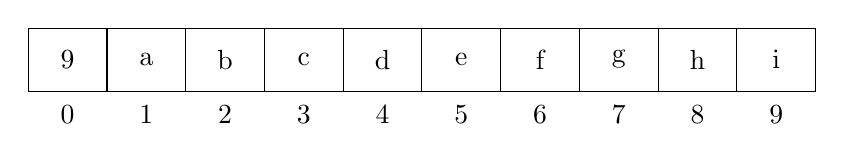
\begin{tikzpicture}
\draw (0,0) rectangle (10,0.8);
\foreach \x in {0,1,2,3,4,5,6,7,8,9}
    \draw (\x,0) -- (\x,0.8);
\node at (0.5,0.4) {9};
\node at (1.5,0.4) {a};
\node at (2.5,0.4) {b};
\node at (3.5,0.4) {c};
\node at (4.5,0.4) {d};
\node at (5.5,0.4) {e};
\node at (6.5,0.4) {f};
\node at (7.5,0.4) {g};
\node at (8.5,0.4) {h};
\node at (9.5,0.4) {i};
\node at (0.5,-0.3) {0};
\node at (1.5,-0.3) {1};
\node at (2.5,-0.3) {2};
\node at (3.5,-0.3) {3};
\node at (4.5,-0.3) {4};
\node at (5.5,-0.3) {5};
\node at (6.5,-0.3) {6};
\node at (7.5,-0.3) {7};
\node at (8.5,-0.3) {8};
\node at (9.5,-0.3) {9};
\end{tikzpicture}
\end{center}

\subsubsection{方法三:用结束符标记}

在串尾存储一个不会在串中出现的特殊字符作为字符串的终结符,例如,在C、C++和Java语言中用'\textbackslash 0'来表示串的结束。

\begin{center}
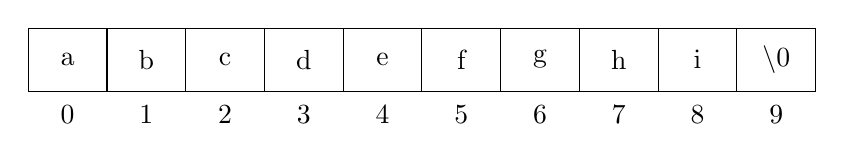
\begin{tikzpicture}
\draw (0,0) rectangle (10,0.8);
\foreach \x in {0,1,2,3,4,5,6,7,8,9}
    \draw (\x,0) -- (\x,0.8);
\node at (0.5,0.4) {a};
\node at (1.5,0.4) {b};
\node at (2.5,0.4) {c};
\node at (3.5,0.4) {d};
\node at (4.5,0.4) {e};
\node at (5.5,0.4) {f};
\node at (6.5,0.4) {g};
\node at (7.5,0.4) {h};
\node at (8.5,0.4) {i};
\node at (9.5,0.4) {\textbackslash 0};
\node at (0.5,-0.3) {0};
\node at (1.5,-0.3) {1};
\node at (2.5,-0.3) {2};
\node at (3.5,-0.3) {3};
\node at (4.5,-0.3) {4};
\node at (5.5,-0.3) {5};
\node at (6.5,-0.3) {6};
\node at (7.5,-0.3) {7};
\node at (8.5,-0.3) {8};
\node at (9.5,-0.3) {9};
\end{tikzpicture}
\end{center}

这种存储方法不能直接得到串的长度,而是通过判断当前字符是否为'\textbackslash 0'来确定串是否结束,从而求得串的长度。

\subsection{字符串的抽象数据类型定义}

字符串的逻辑结构与线性表的逻辑结构相同,但字符串的基本操作和线性表的基本操作有很大差别。线性表的基本操作大多以"单个元素"作为操作对象,而字符串的基本操作通常以"字符串整体"作为操作对象。

\begin{lstlisting}[caption=字符串抽象数据类型]
ADT String {
    数据对象:D = {ai | ai ∈ CharacterSet, i = 1,2,...,n, n ≥ 0}
    数据关系:R1 = {<ai-1, ai> | ai-1, ai ∈ D, i = 2,...,n}
    基本操作:
        StrAssign(T, chars);          // 串赋值
        StrCopy(T, S);               // 串复制
        StrEmpty(S);                 // 判断串空
        StrCompare(S, T);            // 串比较
        StrLength(S);                // 求串长
        StrConcat(T, S1, S2);        // 串连接
        SubString(Sub, S, pos, len); // 求子串
        Index(S, T, pos);            // 子串定位
        Replace(S, T, V);            // 串替换
        StrInsert(S, pos, T);        // 串插入
        StrDelete(S, pos, len);      // 串删除
} ADT String
\end{lstlisting}

\section{模式匹配算法}

模式匹配是字符串处理中最重要的操作之一。给定两个字符串 $S = "s_1s_2\cdots s_n"$ 和 $T = "t_1t_2\cdots t_m"$,在主串 $S$ 中寻找子串 $T$ 的过程称为模式匹配(pattern matching),$T$ 称为模式(pattern)。如果匹配成功,返回 $T$ 在 $S$ 中的位置;如果匹配失败,返回0。

\subsection{BF算法(暴力匹配)}

BF算法(Brute-Force algorithm)的基本思想是蛮力匹配,即从主串 $S$ 的第一个字符开始和模式 $T$ 的第一个字符进行比较。若相等,则继续比较两者的后续字符;否则,从主串 $S$ 的第二个字符开始和模式 $T$ 的第一个字符进行比较。重复上述过程,直至 $S$ 或 $T$ 中所有字符比较完毕。

\begin{algorithm}[H]
\caption{BF算法}
\begin{algorithmic}[1]
\REQUIRE 主串$S$,模式$T$
\ENSURE $T$在$S$中的位置
\STATE $start \leftarrow 0$, $i \leftarrow 0$, $j \leftarrow 0$
\WHILE{$S[i] \neq '\backslash 0'$ AND $T[j] \neq '\backslash 0'$}
    \IF{$S[i] = T[j]$}
        \STATE $i \leftarrow i + 1$, $j \leftarrow j + 1$
    \ELSE
        \STATE $start \leftarrow start + 1$
        \STATE $i \leftarrow start$, $j \leftarrow 0$
    \ENDIF
\ENDWHILE
\IF{$T[j] = '\backslash 0'$}
    \RETURN $start + 1$
\ELSE
    \RETURN $0$
\ENDIF
\end{algorithmic}
\end{algorithm}

\begin{lstlisting}[caption=BF算法C++实现]
int BF(char S[], char T[]) {
    int start = 0;  // 主串从下标0开始第一趟匹配
    int i = 0, j = 0;  // 设置比较的起始下标
    
    while (S[i] != '\0' && T[j] != '\0') {
        if (S[i] == T[j]) {
            i++; j++;  // 继续比较下一对字符
        } else {
            start++;   // 开始下一趟匹配
            i = start; j = 0;  // i和j分别回溯
        }
    }
    
    if (T[j] == '\0')
        return start + 1;  // 返回本趟匹配的起始位置
    else
        return 0;  // 匹配失败
}
\end{lstlisting}

\begin{theorem}[BF算法时间复杂度]
设主串 $S$ 长度为 $n$,模式 $T$ 长度为 $m$,在匹配成功的情况下,考虑两种极端情况:
\begin{enumerate}
\item \textbf{最好情况}:每趟不成功的匹配都发生在模式 $T$ 的第一个字符。平均比较次数为 $\frac{n+m}{2} = O(n+m)$。
\item \textbf{最坏情况}:每趟不成功的匹配都发生在模式 $T$ 的最后一个字符。平均比较次数为 $\frac{m(n-m+2)}{2} = O(n \times m)$。
\item \textbf{平均情况}:$O(n+m)$
\end{enumerate}
其中$n$为主串长度,$m$为模式长度。
\end{theorem}

\begin{example}[BF算法执行过程]
设主串 $S = "abcabcacb"$,模式 $T = "abcac"$,BF算法的匹配过程如下:

\textbf{第1趟匹配:}
\begin{center}
\begin{tabular}{|c|c|c|c|c|c|c|c|c|c|}
\hline
S & a & b & c & a & b & c & a & c & b \\
\hline
T & a & b & c & a & \textcolor{red}{c} &  &  &  &  \\
\hline
\end{tabular}
\end{center}
$i=4, j=4$ 失败,$i$ 回溯到1,$j$ 回溯到0

\textbf{第2趟匹配:}
\begin{center}
\begin{tabular}{|c|c|c|c|c|c|c|c|c|c|}
\hline
S & a & \textcolor{red}{b} & c & a & b & c & a & c & b \\
\hline
T &  & \textcolor{red}{a} &  &  &  &  &  &  &  \\
\hline
\end{tabular}
\end{center}
$i=1, j=0$ 失败,$i$ 回溯到2,$j$ 回溯到0

\textbf{第3趟匹配:}
\begin{center}
\begin{tabular}{|c|c|c|c|c|c|c|c|c|c|}
\hline
S & a & b & \textcolor{red}{c} & a & b & c & a & c & b \\
\hline
T &  &  & \textcolor{red}{a} &  &  &  &  &  &  \\
\hline
\end{tabular}
\end{center}
$i=2, j=0$ 失败,$i$ 回溯到3,$j$ 回溯到0

\textbf{第4趟匹配:}
\begin{center}
\begin{tabular}{|c|c|c|c|c|c|c|c|c|c|}
\hline
S & a & b & c & a & b & c & a & c & b \\
\hline
T &  &  &  & a & b & c & a & c &  \\
\hline
\end{tabular}
\end{center}
$i=8, j=5$,$T$ 中全部字符都比较完毕,匹配成功,返回位置4。
\end{example}

\subsection{KMP算法}

KMP算法是克努思(Knuth)、莫里斯(Morris)和普拉特(Pratt)同时设计的,是对BF算法的重大改进。KMP算法的核心思想是避免主串指针回溯,通过预计算模式的next数组实现高效匹配。

\subsubsection{KMP算法的基本思想}

分析BF算法的执行过程,造成BF算法效率低的原因是回溯,即在某趟匹配失败后,对于主串$S$要回溯到本趟匹配开始字符的下一个字符,模式$T$要回溯到第一个字符,而这些回溯往往是不必要的。

KMP算法希望某趟在$S[i]$和$T[j]$匹配失败后,下标$i$不回溯,下标$j$回溯至某个位置$k$,使得$T[k]$对准$S[i]$继续进行比较。关键问题是如何确定位置$k$。

\begin{definition}[next数组]
模式中的每一个字符$T[j]$都对应一个$k$值,这个$k$值仅依赖于模式本身,与主串无关。用$\text{next}[j]$表示$T[j]$对应的$k$值$(0 \leq j < m)$,其定义如下:
$$\text{next}[j] = \begin{cases}
-1 & j = 0 \\
\max\{k | 1 \leq k < j \text{ 且 } T[0]\cdots T[k-1] = T[j-k]\cdots T[j-1]\} & \text{集合非空} \\
0 & \text{其他情况}
\end{cases}$$
\end{definition}

\textbf{next数组的含义:}
next[j]表示当模式中第j个字符与主串中相应字符"失配"时,在模式中需要重新和主串中该字符进行比较的字符的位置。

\begin{example}[计算next数组]
设模式 $T = "ababc"$,计算其next值:

\begin{center}
\begin{tabular}{|c|c|c|c|c|c|}
\hline
j & 0 & 1 & 2 & 3 & 4 \\
\hline
T[j] & a & b & a & b & c \\
\hline
next[j] & -1 & 0 & 0 & 1 & 2 \\
\hline
\end{tabular}
\end{center}

计算过程:
\begin{itemize}
\item $j=0$: $\text{next}[0] = -1$
\item $j=1$: $\text{next}[1] = 0$
\item $j=2$: $T[0] \neq T[1]$,故 $\text{next}[2] = 0$
\item $j=3$: $T[0] = T[2] = a$,故 $\text{next}[3] = 1$
\item $j=4$: $T[0]T[1] = T[2]T[3] = ab$,故 $\text{next}[4] = 2$
\end{itemize}
\end{example}

\begin{example}[KMP算法执行过程]
设主串 $S = "ababcabcacbab"$,模式 $T = "abcac"$。

首先计算模式T的next数组。`next[j]` 的值是模式串 `T` 的子串 `T[0...j-1]` 的最长公共前后缀的长度。

\begin{center}
\begin{tabular}{|c|c|c|c|c|c|}
\hline
j & 0 & 1 & 2 & 3 & 4 \\
\hline
T[j] & a & b & c & a & c \\
\hline
next[j] & -1 & 0 & 0 & 0 & 1 \\
\hline
\end{tabular}
\end{center}
\textbf{详细计算过程}:
\begin{itemize}
    \item \textbf{j = 0}: 
        \begin{itemize}
            \item `next[0]` 按定义为 -1。这是一个哨兵值,表示模式串的第一个字符就不匹配,此时主串指针需要后移。
        \end{itemize}
    \item \textbf{j = 1}: 
        \begin{itemize}
            \item 子串 `T[0...0]` 为 "a"。
            \item 其所有前缀和后缀都为空。最长公共前后缀长度为0。
            \item 所以 `next[1] = 0`。
        \end{itemize}
    \item \textbf{j = 2}: 
        \begin{itemize}
            \item 子串 `T[0...1]` 为 "ab"。
            \item 前缀: \{"a"\}。后缀: \{"b"\}。
            \item 两者没有交集。最长公共前后缀长度为0。
            \item 所以 `next[2] = 0`。
        \end{itemize}
    \item \textbf{j = 3}: 
        \begin{itemize}
            \item 子串 `T[0...2]` 为 "abc"。
            \item 前缀: \{"a", "ab"\}。后缀: \{"c", "bc"\}。
            \item 两者没有交集。最长公共前后缀长度为0。
            \item 所以 `next[3] = 0`。
        \end{itemize}
    \item \textbf{j = 4}: 
        \begin{itemize}
            \item 子串 `T[0...3]` 为 "abca"。
            \item 前缀: \{"a", "ab", "abc"\}。后缀: \{"a", "ca", "bca"\}。
            \item 最长的公共元素是 "a",长度为1。
            \item 所以 `next[4] = 1`。
        \end{itemize}
\end{itemize}

\textbf{KMP匹配过程} (i为主串指针,j为模式串指针):

\textbf{第1趟匹配:} $i$从0开始, $j$从0开始
\begin{center}
\begin{tabular}{|c|c|c|c|c|c|c|c|c|c|c|c|c|}
\hline
S & a & b & c & a & \textcolor{red}{b} & c & a & c & b & a & b & \\
\hline
T & a & b & c & a & \textcolor{red}{c} &  &  &  &  &  &  &  \\
\hline
索引i & 0 & 1 & 2 & 3 & 4 & 5 & 6 & 7 & 8 & 9 & 10 & 11 \\
\hline
\end{tabular}
\end{center}
在 $i=4, j=4$ 时,$S[4]='b' \neq T[4]='c'$,发生不匹配。\\
根据KMP算法,主串指针$i$不回溯 ($i$保持为4),模式串指针$j$更新为 $j = \text{next}[4] = 1$。

\textbf{第2趟匹配:}
\begin{center}
\begin{tabular}{|c|c|c|c|c|c|c|c|c|c|c|c|c|}
\hline
S & a & b & c & a & \textcolor{red}{b} & c & a & c & b & a & b & \\
\hline
T &   &   &   &   & \textcolor{red}{b} & c & a & c &  &  &  &  \\
\hline
索引i & 0 & 1 & 2 & 3 & 4 & 5 & 6 & 7 & 8 & 9 & 10 & 11 \\
\hline
\end{tabular}
\end{center}
从 $i=4, j=1$ 继续比较。$S[4]='b' = T[1]='b'$,匹配。$i,j$ 都加1。\\
$i=5, j=2$ 时,$S[5]='c' = T[2]='c'$,匹配。$i,j$ 都加1。\\
$i=6, j=3$ 时,$S[6]='a' = T[3]='a'$,匹配。$i,j$ 都加1。\\
$i=7, j=4$ 时,$S[7]='c' = T[4]='c'$,匹配。$i,j$ 都加1。\\
$i=8, j=5$ 时,$T[j]$ 到达末尾($\backslash 0$),说明匹配成功。\\
返回匹配开始的位置 $i-j = 8-5 = 3$ (若从1开始计数,则是位置4)。
\end{example}

\begin{algorithm}
\caption{KMP算法}
\begin{algorithmic}[1]
\REQUIRE 主串$S$,模式$T$,next数组
\ENSURE $T$在$S$中的位置
\STATE $i \leftarrow 0$, $j \leftarrow 0$
\WHILE{$S[i] \neq '\backslash 0'$ AND $T[j] \neq '\backslash 0'$}
    \IF{$S[i] = T[j]$}
        \STATE $i \leftarrow i + 1$, $j \leftarrow j + 1$
    \ELSE
        \STATE $j \leftarrow \text{next}[j]$
        \IF{$j = -1$}
            \STATE $i \leftarrow i + 1$, $j \leftarrow 0$
        \ENDIF
    \ENDIF
\ENDWHILE
\IF{$T[j] = '\backslash 0'$}
    \RETURN $i - j + 1$
\ELSE
    \RETURN $0$
\ENDIF
\end{algorithmic}
\end{algorithm}

\begin{theorem}[KMP算法时间复杂度]
KMP算法的时间复杂度为 $O(n+m)$,其中$n$为主串长度,$m$为模式长度。
\end{theorem}

\section{多维数组}

\subsection{数组的基本概念}

\begin{definition}[数组]
数组是由类型相同的数据元素构成的有序集合,每个元素受$n(n \geq 1)$个线性关系约束,每个元素在$n$个线性关系中的序号称为下标。
\end{definition}

数组的特点:
\begin{itemize}
\item 数据元素类型相同
\item 结构固定,一般不做插入删除操作
\item 支持随机访问
\item 是线性表的推广
\end{itemize}

\subsection{数组的存储结构与寻址}

\subsubsection{二维数组的存储}

二维数组可按两种方式存储:
\begin{itemize}
\item \textbf{按行优先}:先行后列存储
\item \textbf{按列优先}:先列后行存储
\end{itemize}

\begin{theorem}[二维数组按行优先寻址公式]
设二维数组$A[l_1..h_1][l_2..h_2]$,按行优先存储,则元素$a_{ij}$的地址为:
$$\text{LOC}(a_{ij}) = \text{LOC}(a_{l_1l_2}) + [(i-l_1) \times (h_2-l_2+1) + (j-l_2)] \times c$$
其中$c$为每个元素占用的存储单元数。
\end{theorem}

\subsubsection{多维数组的寻址}

对于$n$维数组$A[d_1][d_2]\cdots[d_n]$,按行优先存储,元素$A[i_1][i_2]\cdots[i_n]$的地址为:
$$\text{LOC}(A[i_1][i_2]\cdots[i_n]) = \text{LOC}(A[0][0]\cdots[0]) + \left(\sum_{k=1}^{n} i_k \prod_{j=k+1}^{n} d_j\right) \times c$$

\section{矩阵的压缩存储}

\subsection{特殊矩阵的压缩存储}

\subsubsection{对称矩阵}

对称矩阵满足 $a_{ij} = a_{ji}$,只需存储下三角部分。

\begin{theorem}[对称矩阵寻址公式]
$n$阶对称矩阵按行优先存储下三角部分,元素$a_{ij}$在一维数组中的下标为:
$$k = \begin{cases}
\frac{i(i-1)}{2} + j - 1 & \text{if } i \geq j \\
\frac{j(j-1)}{2} + i - 1 & \text{if } i < j
\end{cases}$$
\end{theorem}

\subsubsection{三角矩阵}

\begin{itemize}
\item \textbf{下三角矩阵}:主对角线以上元素为常数$c$
\item \textbf{上三角矩阵}:主对角线以下元素为常数$c$
\end{itemize}

存储方案:存储非常数元素 + 一个常数。

\subsubsection{对角矩阵(带状矩阵)}

对角矩阵的非零元素集中在主对角线及其附近的几条对角线上。

\begin{example}[三对角矩阵]
三对角矩阵的寻址公式:
$$k = 2i + j - 3 \quad (|i-j| \leq 1)$$
\end{example}

\subsection{稀疏矩阵的存储}

\begin{definition}[稀疏矩阵]
设$m \times n$矩阵中有$t$个非零元素,若$t \ll m \times n$,则称该矩阵为稀疏矩阵。
\end{definition}

稀疏矩阵的存储策略:只存储非零元素,节省存储空间。

\subsubsection{三元组表示法}

三元组$(i, j, v)$表示矩阵第$i$行第$j$列的元素值为$v$。

\begin{lstlisting}[caption=三元组结构定义]
typedef struct {
    int i, j;        // 行号和列号
    ElemType e;      // 元素值
} Triple;

typedef struct {
    Triple data[MAXSIZE];  // 三元组表
    int m, n, t;          // 矩阵的行数、列数和非零元素个数
} TSMatrix;
\end{lstlisting}

\subsubsection{稀疏矩阵的转置}

\textbf{方法一:简单转置算法}

\begin{algorithm}[H]
\caption{简单转置算法}
\begin{algorithmic}[1]
\REQUIRE 稀疏矩阵$A$
\ENSURE 转置矩阵$B$
\STATE $B.m \leftarrow A.n$, $B.n \leftarrow A.m$, $B.t \leftarrow A.t$
\STATE $q \leftarrow 1$
\FOR{$col = 1$ to $A.n$}
    \FOR{$p = 1$ to $A.t$}
        \IF{$A.data[p].j = col$}
            \STATE $B.data[q].i \leftarrow A.data[p].j$
            \STATE $B.data[q].j \leftarrow A.data[p].i$
            \STATE $B.data[q].e \leftarrow A.data[p].e$
            \STATE $q \leftarrow q + 1$
        \ENDIF
    \ENDFOR
\ENDFOR
\end{algorithmic}
\end{algorithm}

\begin{theorem}[简单转置算法时间复杂度]
时间复杂度为$O(n \times t)$,其中$n$为矩阵列数,$t$为非零元素个数。当$t$与$m \times n$同数量级时,算法的时间复杂度为$O(m \times n^2)$。
\end{theorem}

\textbf{方法二:快速转置算法}

利用辅助数组记录每列的非零元素个数和每列第一个非零元素在转置矩阵中的位置。

\begin{algorithm}[H]
\caption{快速转置算法}
\begin{algorithmic}[1]
\REQUIRE 稀疏矩阵$A$
\ENSURE 转置矩阵$B$
\STATE $B.m \leftarrow A.n$, $B.n \leftarrow A.m$, $B.t \leftarrow A.t$
\STATE 初始化$num[1..A.n]$和$cpot[1..A.n]$
\FOR{$col = 1$ to $A.n$}
    \STATE $num[col] \leftarrow 0$
\ENDFOR
\FOR{$t = 1$ to $A.t$}
    \STATE $num[A.data[t].j] \leftarrow num[A.data[t].j] + 1$
\ENDFOR
\STATE $cpot[1] \leftarrow 1$
\FOR{$col = 2$ to $A.n$}
    \STATE $cpot[col] \leftarrow cpot[col-1] + num[col-1]$
\ENDFOR
\FOR{$p = 1$ to $A.t$}
    \STATE $col \leftarrow A.data[p].j$
    \STATE $pos \leftarrow cpot[col]$
    \STATE $B.data[pos] \leftarrow$ 转置$A.data[p]$
    \STATE $cpot[col] \leftarrow cpot[col] + 1$
\ENDFOR
\end{algorithmic}
\end{algorithm}

\begin{theorem}[快速转置算法时间复杂度]
时间复杂度为$O(n + t)$,其中$n$为矩阵列数,$t$为非零元素个数。
\end{theorem}

\subsubsection{十字链表表示法}

对于频繁进行插入、删除操作的稀疏矩阵,三元组表示法效率较低,可采用十字链表表示法。

\begin{lstlisting}[caption=十字链表结构定义]
typedef struct OLNode {
    int i, j;                    // 行号和列号
    ElemType e;                  // 元素值
    struct OLNode *right, *down; // 同行右邻接和同列下邻接
} OLNode, *OLink;

typedef struct {
    OLink *rhead, *chead;  // 行和列链表头指针向量
    int m, n, t;          // 矩阵的行数、列数和非零元素个数
} CrossList;
\end{lstlisting}

十字链表的优点:
\begin{itemize}
\item 能够方便地进行按行或按列遍历
\item 插入和删除操作效率高
\item 适合于矩阵运算
\end{itemize}

\subsubsection{稀疏矩阵转置算法详细示例}

设有如下$6 \times 7$稀疏矩阵$A$,包含7个非零元素:

$$
A = \begin{pmatrix}
0 & 0 & 12 & 0 & 9 & 0 & 0 \\
0 & 0 & 0 & 0 & 0 & 0 & 0 \\
0 & -1 & 0 & 0 & 0 & 0 & 0 \\
5 & 0 & 0 & -3 & 0 & 0 & 0 \\
0 & 0 & 0 & 0 & 0 & 2 & 0 \\
0 & 0 & 0 & 0 & 8 & 0 & 0
\end{pmatrix}
$$

三元组表示为:$A.m = 6$,$A.n = 7$,$A.t = 7$

\begin{center}
\begin{tabular}{|c|c|c|c|}
\hline
p(下标) & i(行) & j(列) & e(值) \\
\hline
1 & 1 & 3 & 12 \\
2 & 1 & 5 & 9 \\
3 & 3 & 2 & -1 \\
4 & 4 & 1 & 5 \\
5 & 4 & 4 & -3 \\
6 & 5 & 6 & 2 \\
7 & 6 & 5 & 8 \\
\hline
\end{tabular}
\end{center}

\textbf{例:简单转置算法执行过程}

初始化:$B.m = 7$,$B.n = 6$,$B.t = 7$,$q = 1$

\begin{enumerate}
\item \textbf{col = 1}:扫描$A.data$,找到$A.data[4]$的$j=1$
    \begin{itemize}
    \item 转置$(4, 1, 5) \rightarrow (1, 4, 5)$
    \item 存入$B.data[1]$,$q = 2$
    \end{itemize}

\item \textbf{col = 2}:扫描$A.data$,找到$A.data[3]$的$j=2$
    \begin{itemize}
    \item 转置$(3, 2, -1) \rightarrow (2, 3, -1)$
    \item 存入$B.data[2]$,$q = 3$
    \end{itemize}

\item \textbf{col = 3}:扫描$A.data$,找到$A.data[1]$的$j=3$
    \begin{itemize}
    \item 转置$(1, 3, 12) \rightarrow (3, 1, 12)$
    \item 存入$B.data[3]$,$q = 4$
    \end{itemize}

\item \textbf{col = 4}:扫描$A.data$,找到$A.data[5]$的$j=4$
    \begin{itemize}
    \item 转置$(4, 4, -3) \rightarrow (4, 4, -3)$
    \item 存入$B.data[4]$,$q = 5$
    \end{itemize}

\item \textbf{col = 5}:扫描$A.data$,找到两个元素$j=5$
    \begin{itemize}
    \item 转置$(1, 5, 9) \rightarrow (5, 1, 9)$,存入$B.data[5]$,$q = 6$
    \item 转置$(6, 5, 8) \rightarrow (5, 6, 8)$,存入$B.data[6]$,$q = 7$
    \end{itemize}

\item \textbf{col = 6}:扫描$A.data$,找到$A.data[6]$的$j=6$
    \begin{itemize}
    \item 转置$(5, 6, 2) \rightarrow (6, 5, 2)$
    \item 存入$B.data[7]$,$q = 8$
    \end{itemize}

\item \textbf{col = 7}:扫描$A.data$,无元素
\end{enumerate}

\textbf{最终结果$B.data$:}

\begin{center}
\begin{tabular}{|c|c|c|c|}
\hline
q(下标) & i(行) & j(列) & e(值) \\
\hline
1 & 1 & 4 & 5 \\
2 & 2 & 3 & -1 \\
3 & 3 & 1 & 12 \\
4 & 4 & 4 & -3 \\
5 & 5 & 1 & 9 \\
6 & 5 & 6 & 8 \\
7 & 6 & 5 & 2 \\
\hline
\end{tabular}
\end{center}

\textbf{例:快速转置算法执行过程}

\textbf{步骤1:计算num数组}

$num[col]$存储$A$的第$col$列的非零元素个数。扫描$A.data$一次:

\begin{center}
\begin{tabular}{|c|c|c|c|c|c|c|c|}
\hline
col & 1 & 2 & 3 & 4 & 5 & 6 & 7 \\
\hline
num & 1 & 1 & 1 & 1 & 2 & 1 & 0 \\
\hline
\end{tabular}
\end{center}

\textbf{步骤2:计算cpot数组}

$cpot[col]$存储$A$的第$col$列元素在$B.data$中的起始位置:

\begin{align}
cpot[1] &= 1 \\
cpot[2] &= cpot[1] + num[1] = 1 + 1 = 2 \\
cpot[3] &= cpot[2] + num[2] = 2 + 1 = 3 \\
cpot[4] &= cpot[3] + num[3] = 3 + 1 = 4 \\
cpot[5] &= cpot[4] + num[4] = 4 + 1 = 5 \\
cpot[6] &= cpot[5] + num[5] = 5 + 2 = 7 \\
cpot[7] &= cpot[6] + num[6] = 7 + 1 = 8
\end{align}

\begin{center}
\begin{tabular}{|c|c|c|c|c|c|c|c|}
\hline
col & 1 & 2 & 3 & 4 & 5 & 6 & 7 \\
\hline
cpot & 1 & 2 & 3 & 4 & 5 & 7 & 8 \\
\hline
\end{tabular}
\end{center}

\textbf{步骤3:放置元素到$B.data$}

最后一次扫描$A.data$,对每个元素$A.data[p]$:

\begin{enumerate}
\item \textbf{p = 1}:$A.data[1] = (1, 3, 12)$,$col=3$,$pos = cpot[3] = 3$
    \begin{itemize}
    \item 放置$(3, 1, 12)$到$B.data[3]$
    \item $cpot[3] \leftarrow 4$
    \end{itemize}

\item \textbf{p = 2}:$A.data[2] = (1, 5, 9)$,$col=5$,$pos = cpot[5] = 5$
    \begin{itemize}
    \item 放置$(5, 1, 9)$到$B.data[5]$
    \item $cpot[5] \leftarrow 6$
    \end{itemize}

\item \textbf{p = 3}:$A.data[3] = (3, 2, -1)$,$col=2$,$pos = cpot[2] = 2$
    \begin{itemize}
    \item 放置$(2, 3, -1)$到$B.data[2]$
    \item $cpot[2] \leftarrow 3$
    \end{itemize}

\item \textbf{p = 4}:$A.data[4] = (4, 1, 5)$,$col=1$,$pos = cpot[1] = 1$
    \begin{itemize}
    \item 放置$(1, 4, 5)$到$B.data[1]$
    \item $cpot[1] \leftarrow 2$
    \end{itemize}

\item \textbf{p = 5}:$A.data[5] = (4, 4, -3)$,$col=4$,$pos = cpot[4] = 4$
    \begin{itemize}
    \item 放置$(4, 4, -3)$到$B.data[4]$
    \item $cpot[4] \leftarrow 5$
    \end{itemize}

\item \textbf{p = 6}:$A.data[6] = (5, 6, 2)$,$col=6$,$pos = cpot[6] = 7$
    \begin{itemize}
    \item 放置$(6, 5, 2)$到$B.data[7]$
    \item $cpot[6] \leftarrow 8$
    \end{itemize}

\item \textbf{p = 7}:$A.data[7] = (6, 5, 8)$,$col=5$,$pos = cpot[5] = 6$
    \begin{itemize}
    \item 放置$(5, 6, 8)$到$B.data[6]$
    \item $cpot[5] \leftarrow 7$
    \end{itemize}
\end{enumerate}

\textbf{最终$B.data$结果:}

\begin{center}
\begin{tabular}{|c|c|c|c|}
\hline
q(下标) & i(行) & j(列) & e(值) \\
\hline
1 & 1 & 4 & 5 \\
2 & 2 & 3 & -1 \\
3 & 3 & 1 & 12 \\
4 & 4 & 4 & -3 \\
5 & 5 & 1 & 9 \\
6 & 5 & 6 & 8 \\
7 & 6 & 5 & 2 \\
\hline
\end{tabular}
\end{center}

两种算法得到相同的结果,但快速转置算法通过预计算避免了重复扫描,大大提高了效率。

\begin{lstlisting}[caption=快速转置算法C++实现]
void FastTranspose(TSMatrix A, TSMatrix &B) {
    B.m = A.n; B.n = A.m; B.t = A.t;
    
    int num[A.n + 1];  // 各列非零元个数
    int cpot[A.n + 1]; // 各列第一个非零元在B中的位置
    
    // 初始化num数组
    for (int col = 1; col <= A.n; col++)
        num[col] = 0;
    
    // 统计各列非零元个数
    for (int t = 1; t <= A.t; t++)
        num[A.data[t].j]++;
    
    // 计算各列第一个非零元在B中的位置
    cpot[1] = 1;
    for (int col = 2; col <= A.n; col++)
        cpot[col] = cpot[col-1] + num[col-1];
    
    // 转置
    for (int p = 1; p <= A.t; p++) {
        int col = A.data[p].j;
        int pos = cpot[col];
        B.data[pos].i = A.data[p].j;
        B.data[pos].j = A.data[p].i;
        B.data[pos].e = A.data[p].e;
        cpot[col]++;
    }
}
\end{lstlisting}

\section{广义表}

\subsection{广义表的定义}

\begin{definition}[广义表]
广义表(Generalized List)是$n(n \geq 0)$个元素的有限序列,记作:
$$LS = (a_1, a_2, \ldots, a_n)$$
其中$LS$是广义表的名称,$a_i$可以是原子或子表。
\end{definition}

\subsection{广义表的特性}

\begin{enumerate}
\item \textbf{有序性}:元素有先后次序
\item \textbf{长度}:最外层包含元素的个数
\item \textbf{深度}:括号的重数
\item \textbf{递归性}:广义表可以为自身的子表
\item \textbf{共享性}:可以被其他广义表所共享
\end{enumerate}

\begin{example}[广义表示例]
\begin{align}
A &= () && \text{空表,长度为0,深度为1} \\
B &= (e) && \text{长度为1,深度为1} \\
C &= (a, (b, c)) && \text{长度为2,深度为2} \\
D &= (a, b, (c, d), e) && \text{长度为4,深度为2} \\
E &= ((a, b), (c, d)) && \text{长度为2,深度为2} \\
F &= (a, F) && \text{递归定义,长度为2,深度无穷}
\end{align}
\end{example}

\subsection{广义表的存储结构}

\subsubsection{头尾链表存储}

\indent

\begin{lstlisting}[caption=头尾链表结构定义]
typedef enum {ATOM, LIST} ElemTag;

typedef struct GLNode {
    ElemTag tag;           // 标志域:ATOM或LIST
    union {
        AtomType atom;     // 原子结点的值域
        struct {
            struct GLNode *hp, *tp;  // 表结点的指针域,hp指向表头,tp指向表尾
        } ptr;
    };
} *GList;
\end{lstlisting}

\subsubsection{子表结点存储}

\indent

\begin{lstlisting}[caption=子表结点结构定义]
typedef struct GLNode {
    ElemTag tag;
    union {
        AtomType atom;
        struct GLNode *hp;  // 指向子表
    };
    struct GLNode *tp;      // 指向同层下一个结点
} *GList;
\end{lstlisting}

\subsection{广义表的基本操作}

\textbf{求广义表的长度:}
\begin{lstlisting}[caption=求广义表长度]
int GListLength(GList L) {
    if (!L) return 0;
    int len = 0;
    while (L) {
        len++;
        L = L->tp;
    }
    return len;
}
\end{lstlisting}

\textbf{求广义表的深度:}
\begin{lstlisting}[caption=求广义表深度]
int GListDepth(GList L) {
    if (!L) return 1;     // 空表深度为1
    if (L->tag == ATOM) return 0;  // 原子深度为0
    
    int maxdep = 0;
    while (L) {
        if (L->tag == LIST) {
            int dep = GListDepth(L->ptr.hp);
            if (dep > maxdep) maxdep = dep;
        }
        L = L->ptr.tp;
    }
    return maxdep + 1;
}
\end{lstlisting}

\subsection{稀疏矩阵的压缩存储}

稀疏矩阵是零元素很多的矩阵,稀疏因子$\delta = \frac{t}{m \times n} < 0.05$。

\subsubsection{三元组顺序表}

将非零元素表示为三元组$(i, j, a_{ij})$,按行优先顺序存储。

\begin{verbatim}
struct Element {
    int row, col;
    DataType value;
};

struct SparseMatrix {
    Element data[MaxSize];
    int rows, cols, nums;  // 行数、列数、非零元个数
};
\end{verbatim}

\subsubsection{十字链表}

每个非零元素节点包含5个域:row, col, value, right, down。
\begin{itemize}
\item right指向同行下一个非零元素
\item down指向同列下一个非零元素
\end{itemize}

\subsection{稀疏矩阵转置算法}

\subsubsection{转置算法1(直接转置)}

\begin{algorithm}
\caption{稀疏矩阵转置算法1}
\begin{algorithmic}[1]
\REQUIRE 稀疏矩阵$A$
\ENSURE 转置矩阵$B$
\STATE 设置$B$的行数、列数、非零元个数
\FOR{$col = 1$ to $A.cols$}
    \FOR{$i = 0$ to $A.nums-1$}
        \IF{$A.data[i].col = col$}
            \STATE 将$A.data[i]$行列交换后存入$B$
        \ENDIF
    \ENDFOR
\ENDFOR
\end{algorithmic}
\end{algorithm}

时间复杂度:$O(cols \times nums)$

\subsubsection{转置算法2(快速转置)}

引入辅助数组:
\begin{itemize}
\item $num[1..A.n]$:第$col$列非零元个数
\item $cpot[1..A.n]$:第$col$列第一个非零元在$B$中的位置
\end{itemize}

递推关系:
$$\begin{cases}
cpot[1] = 0 \\
cpot[col] = cpot[col-1] + num[col-1] \quad (2 \leq col \leq nu)
\end{cases}$$

\begin{algorithm}
\caption{稀疏矩阵转置算法2}
\begin{algorithmic}[1]
\REQUIRE 稀疏矩阵$A$
\ENSURE 转置矩阵$B$
\STATE 统计每列非零元个数到$num[]$
\STATE 计算每列第一个元素在$B$中位置到$cpot[]$
\FOR{$i = 0$ to $A.nums-1$}
    \STATE $col \leftarrow A.data[i].col$
    \STATE $pos \leftarrow cpot[col]$
    \STATE $B.data[pos] \leftarrow$ 转置$A.data[i]$
    \STATE $cpot[col] \leftarrow cpot[col] + 1$
\ENDFOR
\end{algorithmic}
\end{algorithm}

时间复杂度:$O(cols + nums)$

\section{重难点分析}

\subsection{重点内容}
\begin{enumerate}
\item \textbf{模式匹配算法}(★★★★★)
    \begin{itemize}
    \item BF算法的执行过程和复杂度分析
    \item KMP算法的next数组计算
    \item KMP算法的匹配过程
    \end{itemize}
    
\item \textbf{数组寻址公式}(★★★★☆)
    \begin{itemize}
    \item 二维数组按行/列优先的寻址公式
    \item 多维数组的寻址公式推导
    \end{itemize}
    
\item \textbf{特殊矩阵压缩存储}(★★★★☆)
    \begin{itemize}
    \item 对称矩阵的存储和寻址
    \item 三角矩阵的存储方案
    \item 对角矩阵的压缩存储
    \end{itemize}
\end{enumerate}

\subsection{难点内容}
\begin{enumerate}
\item \textbf{KMP算法的next数组计算}(★★★★★)
    \begin{itemize}
    \item 理解next数组的含义
    \item 掌握手工计算next值的方法
    \item 理解KMP算法避免回溯的原理
    \end{itemize}
    
\item \textbf{稀疏矩阵的压缩存储}(★★★★☆)
    \begin{itemize}
    \item 三元组表的组织方式
    \item 十字链表的结构设计
    \item 稀疏矩阵转置算法的优化
    \end{itemize}
\end{enumerate}


\section{典型例题}

\begin{example}[KMP算法next数组计算]
设模式串$T = "abcabca"$,求其next数组。

\textbf{解答:}
\begin{center}
\begin{tabular}{|c|c|c|c|c|c|c|c|}
\hline
j & 0 & 1 & 2 & 3 & 4 & 5 & 6 \\
\hline
T[j] & a & b & c & a & b & c & a \\
\hline
next[j] & -1 & 0 & 0 & 0 & 1 & 2 & 3 \\
\hline
\end{tabular}
\end{center}

计算过程:
\begin{itemize}
\item $j=0$: $\text{next}[0] = -1$
\item $j=1$: $\text{next}[1] = 0$
\item $j=2$: $T[0] \neq T[1]$,$\text{next}[2] = 0$
\item $j=3$: $T[0] \neq T[1] \neq T[2]$,$\text{next}[3] = 0$
\item $j=4$: $T[0] = T[3] = a$,$\text{next}[4] = 1$
\item $j=5$: $T[0]T[1] = T[3]T[4] = ab$,$\text{next}[5] = 2$
\item $j=6$: $T[0]T[1]T[2] = T[3]T[4]T[5] = abc$,$\text{next}[6] = 3$
\end{itemize}
\end{example}

\begin{example}[对称矩阵压缩存储]
设有5阶对称矩阵,按行优先存储下三角部分,求元素$a_{32}$和$a_{23}$在一维数组中的下标。

\textbf{解答:}
对于$a_{32}$($i=3, j=2$),由于$i > j$,直接计算:
$$k = \frac{i(i-1)}{2} + j - 1 = \frac{3 \times 2}{2} + 2 - 1 = 4$$

对于$a_{23}$($i=2, j=3$),由于$i < j$,利用对称性$a_{23} = a_{32}$:
$$k = \frac{j(j-1)}{2} + i - 1 = \frac{3 \times 2}{2} + 2 - 1 = 4$$

因此两个元素都存储在下标4的位置。
\end{example}

\begin{example}[二维数组寻址]
设有二维数组$A[1..10][5..15]$,每个元素占4个字节,按行优先存储,数组首地址为1000,求$A[5][8]$的地址。

\textbf{解答:}
按行优先寻址公式:
$$\text{LOC}(A[i][j]) = \text{LOC}(A[1][5]) + [(i-1) \times (15-5+1) + (j-5)] \times 4$$

代入$i=5, j=8$:
$$\text{LOC}(A[5][8]) = 1000 + [(5-1) \times 11 + (8-5)] \times 4$$
$$= 1000 + (44 + 3) \times 4 = 1000 + 188 = 1188$$
\end{example}

\section{复习建议}

\subsection{学习重点顺序}
\begin{enumerate}
\item \textbf{第一轮:掌握基本概念}
    \begin{itemize}
    \item 字符串的定义和存储方式
    \item 数组的寻址计算方法
    \item 矩阵压缩存储的基本思想
    \end{itemize}
    
\item \textbf{第二轮:理解核心算法}
    \begin{itemize}
    \item BF算法的执行过程
    \item KMP算法的next数组计算
    \item 稀疏矩阵的转置算法
    \end{itemize}
    
\item \textbf{第三轮:强化练习}
    \begin{itemize}
    \item 大量next数组计算练习
    \item 各种寻址公式的推导和应用
    \item 算法复杂度分析
    \end{itemize}
\end{enumerate}

\subsection{常考题型}
\begin{enumerate}
\item \textbf{选择题}:算法复杂度、存储效率、概念理解
\item \textbf{填空题}:next数组数值、寻址公式结果、复杂度表达式
\item \textbf{应用题}:手工执行算法、公式推导、程序设计
\item \textbf{算法题}:KMP算法实现、矩阵操作算法
\end{enumerate}

\subsection{记忆要点}
\begin{enumerate}
\item \textbf{KMP算法}:
    \begin{itemize}
    \item next[0] = -1, next[1] = 0
    \item 寻找最长相同前缀后缀
    \item 时间复杂度O(m+n)
    \end{itemize}
    
\item \textbf{寻址公式}:
    \begin{itemize}
    \item 二维数组:LOC = base + (i×列数 + j)×size
    \item 对称矩阵:k = i(i-1)/2 + j - 1(i≥j)
    \item 三角矩阵:存储方式决定公式形式
    \end{itemize}
    
\item \textbf{复杂度}:
    \begin{itemize}
    \item BF算法:最坏O(mn),平均O(m+n)
    \item KMP算法:O(m+n)
    \item 矩阵转置:简单O(列数×非零元),快速O(列数+非零元)
    \end{itemize}
\end{enumerate}

\section{扩展知识}

\subsection{高级字符串算法}
\begin{itemize}
\item \textbf{Boyer-Moore算法}:从右向左匹配,使用坏字符和好后缀规则
\item \textbf{Sunday算法}:BM算法的简化版本,使用坏字符规则
\item \textbf{Rabin-Karp算法}:基于哈希值的匹配算法
\item \textbf{AC自动机}:多模式串匹配,基于KMP和字典树
\end{itemize}

\subsection{现代应用}
\begin{itemize}
\item \textbf{文本编辑器}:查找替换功能的核心算法
\item \textbf{生物信息学}:DNA序列分析中的模式匹配
\item \textbf{信息检索}:搜索引擎中的字符串匹配
\item \textbf{网络安全}:入侵检测系统中的模式识别
\end{itemize}

\subsection{相关数据结构}
\begin{itemize}
\item \textbf{字典树(Trie)}:高效的字符串存储和检索
\item \textbf{后缀数组}:字符串处理的强大工具
\item \textbf{后缀树}:线性时间的多种字符串操作
\item \textbf{压缩索引}:大数据时代的字符串索引技术
\end{itemize}

\section{总结}

字符串和多维数组是数据结构中的重要内容,具有很强的实用性。学习重点包括:

\begin{enumerate}
\item \textbf{理论基础}:深入理解各种算法的原理和适用场景
\item \textbf{算法实现}:熟练掌握关键算法的实现细节
\item \textbf{复杂度分析}:能够准确分析算法的时间空间复杂度
\item \textbf{实际应用}:了解这些数据结构在实际项目中的应用
\end{enumerate}

通过系统学习和大量练习,相信同学们能够很好地掌握这部分内容,为后续课程和实际应用打下坚实基础。

\end{document}

\section{复习建议}

\begin{mdframed}[style=framestyle]
\subsection{学习重点}
\begin{enumerate}
\item \textbf{熟练掌握KMP算法}
    \begin{itemize}
    \item 多练习next数组的手工计算
    \item 理解KMP算法的匹配过程
    \item 掌握算法的时间复杂度分析
    \end{itemize}
    
\item \textbf{掌握数组寻址公式}
    \begin{itemize}
    \item 记忆二维数组的寻址公式
    \item 理解行优先和列优先的区别
    \item 练习多维数组的寻址计算
    \end{itemize}
    
\item \textbf{掌握矩阵压缩存储}
    \begin{itemize}
    \item 理解各种特殊矩阵的特点
    \item 掌握压缩存储的寻址方法
    \item 理解稀疏矩阵的存储结构
    \end{itemize}
\end{enumerate}

\subsection{常考题型}
\begin{enumerate}
\item KMP算法的next数组计算
\item 数组元素的寻址计算
\item 特殊矩阵的压缩存储方案
\item 稀疏矩阵的存储结构设计
\item 字符串基本操作的实现
\end{enumerate}
\end{mdframed}

\section{扩展知识}

\subsection{字符串匹配的其他算法}
\begin{itemize}
\item \textbf{Boyer-Moore算法}:从右向左匹配,利用坏字符和好后缀规则
\item \textbf{Rabin-Karp算法}:基于哈希的字符串匹配
\item \textbf{Sunday算法}:BM算法的简化版本
\end{itemize}

\subsection{多维数组的应用}
\begin{itemize}
\item \textbf{图像处理}:二维数组表示图像像素
\item \textbf{科学计算}:多维数组表示张量
\item \textbf{动态规划}:多维数组存储状态
\end{itemize}

\subsection{压缩存储的实际应用}
\begin{itemize}
\item \textbf{大规模科学计算}:稀疏矩阵运算
\item \textbf{图论算法}:邻接矩阵的压缩存储
\item \textbf{机器学习}:特征矩阵的稀疏表示
\end{itemize}

\end{document} 
% \documentclass[12pt,a4paper]{amsart}
\usepackage[utf8]{inputenc}
\usepackage[T1]{fontenc}
\usepackage{amsmath,amsfonts,amssymb}
\usepackage{tikz}
\usepackage{algorithm}
\usepackage{algorithmic}
\usepackage{float}
\usepackage{listings}
\usepackage{xcolor}
\usepackage{geometry}
\usepackage{fancyhdr}
\usepackage{enumitem}
\usepackage{booktabs}
\usepackage{multirow}
\usepackage[hidelinks,bookmarksnumbered,bookmarksopen]{hyperref}
\usepackage{xeCJK}
\setCJKmainfont{LXGW WenKai}

\geometry{left=2.5cm,right=2.5cm,top=2.5cm,bottom=2.5cm}

% 代码高亮设置
\lstset{
    language=C++,
    basicstyle=\ttfamily\small,
    keywordstyle=\color{blue}\bfseries,
    commentstyle=\color{green!60!black},
    stringstyle=\color{red},
    numbers=left,
    numberstyle=\tiny\color{gray},
    stepnumber=1,
    numbersep=10pt,
    backgroundcolor=\color{gray!10},
    frame=single,
    tabsize=4,
    captionpos=b,
    breaklines=true,
    breakatwhitespace=false,
    showspaces=false,
    showstringspaces=false,
    showtabs=false
}

% 定理环境
\newtheorem{definition}{定义}[section]
\newtheorem{theorem}{定理}[section]

\newtheorem{example}{例题}[section]
\newtheorem{property}{性质}[section]

% TikZ库
\usetikzlibrary{trees,positioning,arrows,automata,calc}

\title{\textbf{数据结构 - 二叉树复习资料}}
\author{详细版本}
\date{\today}

\begin{document}

% \maketitle

% % 目录设置
% \tableofcontents
% \newpage

\section{二叉树的基本概念}

\subsection{树和二叉树的定义}

\begin{definition}[树]
树是$n(n \geq 0)$个结点的有限集合。当$n=0$时,称为空树;任意一棵非空树满足以下条件:
\begin{enumerate}
\item 有且仅有一个特定的称为根的结点;
\item 当$n>1$时,除根结点之外的其余结点被分成$m(m>0)$个互不相交的有限集合$T_1, T_2, \ldots, T_m$,其中每个集合又是一棵树,并称为这个根结点的子树。
\end{enumerate}
\end{definition}

\begin{definition}[二叉树]
二叉树是$n(n \geq 0)$个结点的有限集合,该集合或者为空集(称为空二叉树),或者由一个根结点和两棵互不相交的、分别称为根结点的左子树和右子树的二叉树组成。
\end{definition}

\subsection{二叉树的特点}

二叉树具有以下特点:
\begin{enumerate}
\item 每个结点最多有两棵子树,所以二叉树中不存在度大于2的结点;
\item 二叉树的左右子树不能任意颠倒,如果某结点只有一棵子树,一定要指明它是左子树还是右子树。
\end{enumerate}

\subsection{特殊的二叉树}

\begin{definition}[满二叉树]
在一棵二叉树中,如果所有分支结点都存在左子树和右子树,并且所有叶子都在同一层上,这样的二叉树称为满二叉树。
\end{definition}

\begin{definition}[完全二叉树]
对一棵具有$n$个结点的二叉树按层序编号,如果编号为$i(1 \leq i \leq n)$的结点与同样深度的满二叉树中编号为$i$的结点在二叉树中的位置完全相同,则这棵二叉树称为完全二叉树。
\end{definition}

\begin{center}
\begin{tikzpicture}[level distance=1.5cm,
level 1/.style={sibling distance=4cm},
level 2/.style={sibling distance=2cm},
level 3/.style={sibling distance=1.5cm}]

% 满二叉树示例
\node at (-4,3) {\textbf{满二叉树}};
\node[circle,draw] at (-4,2) {1}
    child {node[circle,draw] {2}
        child {node[circle,draw] {4}}
        child {node[circle,draw] {5}}}
    child {node[circle,draw] {3}
        child {node[circle,draw] {6}}
        child {node[circle,draw] {7}}};

% 完全二叉树示例
\node at (4,3) {\textbf{完全二叉树}};
\node[circle,draw] at (4,2) {1}
    child {node[circle,draw] {2}
        child {node[circle,draw] {4}}
        child {node[circle,draw] {5}}}
    child {node[circle,draw] {3}
        child {node[circle,draw] {6}}
        child[missing]};
\end{tikzpicture}
\end{center}

\section{二叉树的基本性质}

\begin{property}[性质1]
在一棵二叉树中,如果叶子结点的个数为$n_0$,度为2的结点个数为$n_2$,则$n_0 = n_2 + 1$。
\end{property}

\begin{proof}
设二叉树的结点总数为$N$,叶子结点(度为0)的个数为$n_0$,度为1的结点个数为$n_1$,度为2的结点个数为$n_2$。
根据定义,树中任意一个结点,其度数(即子结点数)只能是0, 1或2。因此,结点总数可以表示为:
$$N = n_0 + n_1 + n_2 \quad (1)$$

现在,我们从两个不同的角度来考虑树中的分枝(边)的总数,设为$B$。

\textbf{角度一:从结点与边的关系来看}
对于一棵非空树,除了根结点,每个结点都有且仅有一个父结点,对应一条进入该结点的分枝。因此,分枝总数等于结点总数减1。
$$B = N - 1 \quad (2)$$

\textbf{角度二:从结点度数与边的关系来看}
树中所有分枝都是由度为1或度为2的结点发出的。每个度为1的结点发出一条分枝,每个度为2的结点发出两条分枝。因此,分枝总数等于所有结点的度数之和。
$$B = (0 \cdot n_0) + (1 \cdot n_1) + (2 \cdot n_2) = n_1 + 2n_2 \quad (3)$$

联立等式 (2) 和 (3),我们得到:
$$N - 1 = n_1 + 2n_2$$
将等式 (1) 代入上式,用 $n_0 + n_1 + n_2$ 替换 $N$:
$$(n_0 + n_1 + n_2) - 1 = n_1 + 2n_2$$
对上式进行化简,两边同时减去 $n_1$:
$$n_0 + n_2 - 1 = 2n_2$$
两边再同时减去 $n_2$:
$$n_0 - 1 = n_2$$
最终得到:
$$n_0 = n_2 + 1$$
此性质对于空树也成立(此时 $n_0=0, n_2=0$)。
\end{proof}

\begin{property}[性质2]
二叉树的第$i$层上最多有$2^{i-1}$个结点$(i \geq 1)$。
\end{property}

\begin{property}[性质3]
在一棵深度为$k$的二叉树中,最多有$2^k - 1$个结点。
\end{property}

\begin{property}[性质4]
具有$n$个结点的完全二叉树的深度为$\lfloor\log_2 n\rfloor + 1$。
\end{property}

\begin{property}[性质5]
对一棵具有$n$个结点的完全二叉树从1开始按层序编号,则对于编号为$i(1 \leq i \leq n)$的结点,有如下关系成立:
\begin{enumerate}
\item 如果$i > 1$,则结点$i$的双亲的编号为$\lfloor i/2 \rfloor$;否则结点$i$是根结点,无双亲。
\item 如果$2i \leq n$,则结点$i$的左孩子的编号为$2i$;否则结点$i$无左孩子。
\item 如果$2i+1 \leq n$,则结点$i$的右孩子的编号为$2i+1$;否则结点$i$无右孩子。
\end{enumerate}
\end{property}

\section{二叉树的存储结构}

\subsection{顺序存储结构}

二叉树的顺序存储结构是用一维数组存储二叉树的结点,用结点的存储位置(下标)表示结点之间的逻辑关系。

\begin{center}
\begin{tikzpicture}[level distance=1.2cm,
level 1/.style={sibling distance=3cm},
level 2/.style={sibling distance=1.5cm},
level 3/.style={sibling distance=1cm}]

\node[circle,draw] (1) {A}
    child {node[circle,draw] (2) {B}
        child[missing]
        child {node[circle,draw] (5) {D}
            child {node[circle,draw] (10) {F}}
            child[missing]}}
    child {node[circle,draw] (3) {C}
        child {node[circle,draw] (6) {E}}
        child[missing]};

% 添加编号
\node[below=0.3cm of 1] {1};
\node[below=0.3cm of 2] {2};
\node[below=0.3cm of 3] {3};
\node[below=0.3cm of 5] {5};
\node[below=0.3cm of 6] {6};
\node[below=0.3cm of 10] {10};
\end{tikzpicture}
\end{center}

顺序存储数组:
\begin{center}
\begin{tabular}{|c|c|c|c|c|c|c|c|c|c|c|}
\hline
下标 & 1 & 2 & 3 & 4 & 5 & 6 & 7 & 8 & 9 & 10 \\
\hline
元素 & A & B & C & $\emptyset$ & D & E & $\emptyset$ & $\emptyset$ & $\emptyset$ & F \\
\hline
\end{tabular}
\end{center}

\subsection{二叉链表}

二叉链表的结点结构:
\begin{center}
\begin{tabular}{|c|c|c|}
\hline
lchild & data & rchild \\
\hline
\end{tabular}
\end{center}

\begin{lstlisting}[caption=二叉链表结点定义]
template <typename DataType>
struct BiNode {
    DataType data;
    BiNode<DataType> *lchild, *rchild;
};
\end{lstlisting}

\section{二叉树的遍历}

\subsection{遍历方法}

二叉树的遍历是指从根结点出发,按照某种次序访问二叉树中的所有结点,使得每个结点被访问一次且仅被访问一次。

\begin{definition}[前序遍历]
若二叉树为空,则空操作返回;否则执行下述操作:
\begin{enumerate}
\item 访问根结点;
\item 前序遍历根结点的左子树;
\item 前序遍历根结点的右子树。
\end{enumerate}
\end{definition}

\begin{definition}[中序遍历]
若二叉树为空,则空操作返回;否则执行下述操作:
\begin{enumerate}
\item 中序遍历根结点的左子树;
\item 访问根结点;
\item 中序遍历根结点的右子树。
\end{enumerate}
\end{definition}

\begin{definition}[后序遍历]
若二叉树为空,则空操作返回;否则执行下述操作:
\begin{enumerate}
\item 后序遍历根结点的左子树;
\item 后序遍历根结点的右子树;
\item 访问根结点。
\end{enumerate}
\end{definition}

\begin{definition}[层序遍历]
从二叉树的根结点开始,从上至下逐层遍历,同一层按从左到右的顺序对结点逐个访问。
\end{definition}

\subsection{遍历算法实现}

\noindent

\begin{algorithm}[H]
\caption{前序遍历递归算法}
\begin{algorithmic}[1]
\REQUIRE 二叉树根指针$bt$
\ENSURE 输出前序遍历序列
\IF{$bt \neq NULL$}
\STATE 访问$bt$的数据域
\STATE 前序遍历$bt$的左子树
\STATE 前序遍历$bt$的右子树
\ENDIF
\end{algorithmic}
\end{algorithm}

\begin{lstlisting}[caption=前序遍历递归实现]
template <typename DataType>
void PreOrder(BiNode<DataType> *bt) {
    if (bt == nullptr) return;
    cout << bt->data << "\t";    // 访问根结点
    PreOrder(bt->lchild);        // 遍历左子树
    PreOrder(bt->rchild);        // 遍历右子树
}
\end{lstlisting}

\begin{example}[前序遍历示例]
给定如下二叉树:
\begin{center}
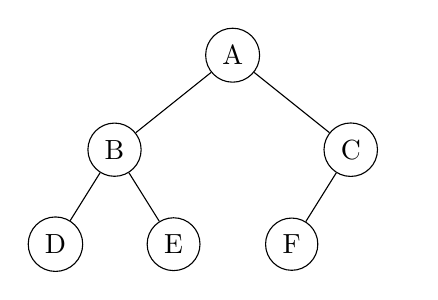
\begin{tikzpicture}[level distance=1.2cm,
    level 1/.style={sibling distance=3cm},
    level 2/.style={sibling distance=1.5cm},
    level 3/.style={sibling distance=1cm}]
\node[circle,draw] {A}
    child {node[circle,draw] {B}
        child {node[circle,draw] {D}}
        child {node[circle,draw] {E}}
    }
    child {node[circle,draw] {C}
        child {node[circle,draw] {F}}
        child {edge from parent[draw=none]}
    };
\end{tikzpicture}
\end{center}

前序遍历过程:
\begin{enumerate}
\item 访问根结点A,输出A
\item 前序遍历左子树(以B为根):
    \begin{itemize}
    \item 访问B,输出B
    \item 前序遍历B的左子树:访问D,输出D
    \item 前序遍历B的右子树:访问E,输出E
    \end{itemize}
\item 前序遍历右子树(以C为根):
    \begin{itemize}
    \item 访问C,输出C
    \item 前序遍历C的左子树:访问F,输出F
    \item 前序遍历C的右子树:空
    \end{itemize}
\end{enumerate}

\textbf{前序遍历结果:A B D E C F}
\end{example}

\begin{algorithm}[H]
\caption{中序遍历递归算法}
\begin{algorithmic}[1]
\REQUIRE 二叉树根指针$bt$
\ENSURE 输出中序遍历序列
\IF{$bt \neq NULL$}
\STATE 中序遍历$bt$的左子树
\STATE 访问$bt$的数据域
\STATE 中序遍历$bt$的右子树
\ENDIF
\end{algorithmic}
\end{algorithm}

\begin{lstlisting}[caption=中序遍历递归实现]
template <typename DataType>
void InOrder(BiNode<DataType> *bt) {
    if (bt == nullptr) return;
    InOrder(bt->lchild);         // 遍历左子树
    cout << bt->data << "\t";    // 访问根结点
    InOrder(bt->rchild);         // 遍历右子树
}
\end{lstlisting}
\begin{center}
    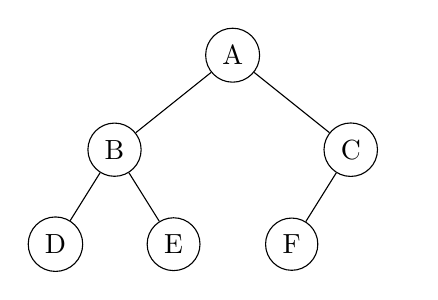
\begin{tikzpicture}[level distance=1.2cm,
        level 1/.style={sibling distance=3cm},
        level 2/.style={sibling distance=1.5cm},
        level 3/.style={sibling distance=1cm}]
    \node[circle,draw] {A}
        child {node[circle,draw] {B}
            child {node[circle,draw] {D}}
            child {node[circle,draw] {E}}
        }
        child {node[circle,draw] {C}
            child {node[circle,draw] {F}}
            child {edge from parent[draw=none]}
        };
    \end{tikzpicture}
    \end{center}
\begin{example}[中序遍历示例]
使用同一棵二叉树,中序遍历过程:
\begin{enumerate}
\item 中序遍历左子树(以B为根):
    \begin{itemize}
    \item 中序遍历B的左子树:访问D,输出D
    \item 访问B,输出B
    \item 中序遍历B的右子树:访问E,输出E
    \end{itemize}
\item 访问根结点A,输出A
\item 中序遍历右子树(以C为根):
    \begin{itemize}
    \item 中序遍历C的左子树:访问F,输出F
    \item 访问C,输出C
    \item 中序遍历C的右子树:空
    \end{itemize}
\end{enumerate}

\textbf{中序遍历结果:D B E A F C}
\end{example}

\begin{algorithm}[H]
\caption{后序遍历递归算法}
\begin{algorithmic}[1]
\REQUIRE 二叉树根指针$bt$
\ENSURE 输出后序遍历序列
\IF{$bt \neq NULL$}
\STATE 后序遍历$bt$的左子树
\STATE 后序遍历$bt$的右子树
\STATE 访问$bt$的数据域
\ENDIF
\end{algorithmic}
\end{algorithm}

\begin{lstlisting}[caption=后序遍历递归实现]
template <typename DataType>
void PostOrder(BiNode<DataType> *bt) {
    if (bt == nullptr) return;
    PostOrder(bt->lchild);       // 遍历左子树
    PostOrder(bt->rchild);       // 遍历右子树
    cout << bt->data << "\t";    // 访问根结点
}
\end{lstlisting}
\begin{center}
    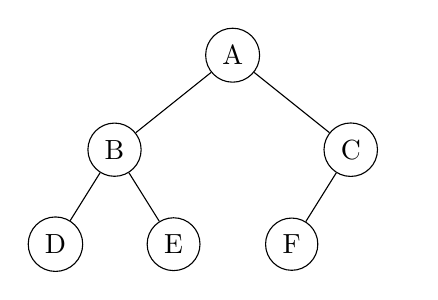
\begin{tikzpicture}[level distance=1.2cm,
        level 1/.style={sibling distance=3cm},
        level 2/.style={sibling distance=1.5cm},
        level 3/.style={sibling distance=1cm}]
    \node[circle,draw] {A}
        child {node[circle,draw] {B}
            child {node[circle,draw] {D}}
            child {node[circle,draw] {E}}
        }
        child {node[circle,draw] {C}
            child {node[circle,draw] {F}}
            child {edge from parent[draw=none]}
        };
    \end{tikzpicture}
    \end{center}
\begin{example}[后序遍历示例]
使用同一棵二叉树,后序遍历过程:
\begin{enumerate}
\item 后序遍历左子树(以B为根):
    \begin{itemize}
    \item 后序遍历B的左子树:访问D,输出D
    \item 后序遍历B的右子树:访问E,输出E
    \item 访问B,输出B
    \end{itemize}
\item 后序遍历右子树(以C为根):
    \begin{itemize}
    \item 后序遍历C的左子树:访问F,输出F
    \item 后序遍历C的右子树:空
    \item 访问C,输出C
    \end{itemize}
\item 访问根结点A,输出A
\end{enumerate}

\textbf{后序遍历结果:D E B F C A}
\end{example}

\begin{example}[更复杂的遍历示例]
考虑一个更复杂的二叉树:
\begin{center}
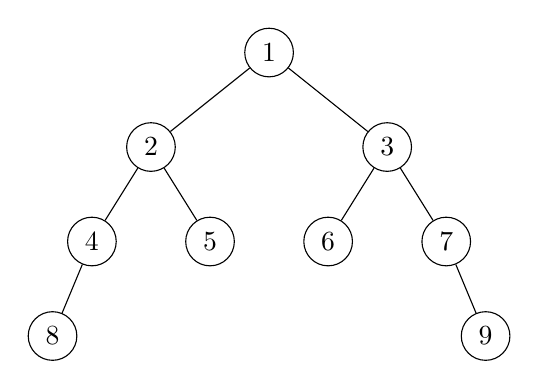
\begin{tikzpicture}[level distance=1.2cm,
    level 1/.style={sibling distance=3cm},
    level 2/.style={sibling distance=1.5cm},
    level 3/.style={sibling distance=1cm}]
\node[circle,draw] {1}
    child {node[circle,draw] {2}
        child {node[circle,draw] {4}
            child {node[circle,draw] {8}}
            child[missing]
        }
        child {node[circle,draw] {5}}
    }
    child {node[circle,draw] {3}
        child {node[circle,draw] {6}}
        child {node[circle,draw] {7}
            child[missing]
            child {node[circle,draw] {9}}
        }
    };
\end{tikzpicture}
\end{center}

\textbf{三种遍历结果比较:}
\begin{itemize}
\item \textbf{前序遍历:}1 2 4 8 5 3 6 7 9
\item \textbf{中序遍历:}8 4 2 5 1 6 3 7 9
\item \textbf{后序遍历:}8 4 5 2 6 9 7 3 1
\end{itemize}

\textbf{规律总结:}
\begin{itemize}
\item 前序遍历:根结点总是在对应子树的最前面
\item 中序遍历:根结点总是在其左右子树之间
\item 后序遍历:根结点总是在对应子树的最后面
\end{itemize}
\end{example}

\subsection{非递归遍历算法}

\indent

\begin{algorithm}[H]
\caption{前序遍历非递归算法}
\begin{algorithmic}[1]
\REQUIRE 二叉树根指针$bt$
\ENSURE 输出前序遍历序列
\STATE 初始化栈$S$
\IF{二叉树非空}
    \STATE 将根指针$bt$入栈
    \WHILE{栈$S$不为空}
        \STATE $p \leftarrow$ 栈顶元素出栈
        \STATE 访问结点$p$的数据域
        \IF{结点$p$存在右孩子}
            \STATE 将右孩子指针入栈
        \ENDIF
        \IF{结点$p$存在左孩子}
            \STATE 将左孩子指针入栈
        \ENDIF
    \ENDWHILE
\ENDIF
\end{algorithmic}
\end{algorithm}

\begin{lstlisting}[caption=前序遍历非递归实现]
template <typename DataType>
void PreOrderNonRecur(BiNode<DataType> *bt) {
    if (bt == nullptr) return;
    stack<BiNode<DataType>*> S;
    S.push(bt);
    
    while (!S.empty()) {
        BiNode<DataType> *p = S.top();
        S.pop();
        cout << p->data << "\t";    // 访问结点
        
        if (p->rchild != nullptr)   // 右孩子先入栈
            S.push(p->rchild);
        if (p->lchild != nullptr)   // 左孩子后入栈(先出栈)
            S.push(p->lchild);
    }
}
\end{lstlisting}

\begin{algorithm}[H]
\caption{中序遍历非递归算法}
\begin{algorithmic}[1]
\REQUIRE 二叉树根指针$bt$
\ENSURE 输出中序遍历序列
\STATE 初始化栈$S$
\STATE $p \leftarrow bt$
\WHILE{$p \neq NULL$ OR 栈$S$不为空}
    \WHILE{$p \neq NULL$}
        \STATE 将$p$入栈
        \STATE $p \leftarrow p$的左孩子
    \ENDWHILE
    \IF{栈$S$不为空}
        \STATE $p \leftarrow$ 栈顶元素出栈
        \STATE 访问结点$p$的数据域
        \STATE $p \leftarrow p$的右孩子
    \ENDIF
\ENDWHILE
\end{algorithmic}
\end{algorithm}

\begin{lstlisting}[caption=中序遍历非递归实现]
template <typename DataType>
void InOrderNonRecur(BiNode<DataType> *bt) {
    stack<BiNode<DataType>*> S;
    BiNode<DataType> *p = bt;
    
    while (p != nullptr || !S.empty()) {
        while (p != nullptr) {      // 一直向左走到底
            S.push(p);
            p = p->lchild;
        }
        if (!S.empty()) {
            p = S.top();
            S.pop();
            cout << p->data << "\t";    // 访问结点
            p = p->rchild;              // 转向右子树
        }
    }
}
\end{lstlisting}

\begin{algorithm}[H]
\caption{后序遍历非递归算法}
\begin{algorithmic}[1]
\REQUIRE 二叉树根指针$bt$
\ENSURE 输出后序遍历序列
\STATE 初始化栈$S$
\STATE $p \leftarrow bt$, $r \leftarrow NULL$
\WHILE{$p \neq NULL$ OR 栈$S$不为空}
    \IF{$p \neq NULL$}
        \STATE 将$p$入栈
        \STATE $p \leftarrow p$的左孩子
    \ELSE
        \STATE $p \leftarrow$ 栈顶元素(不出栈)
        \IF{$p$的右孩子存在且$p$的右孩子$\neq r$}
            \STATE $p \leftarrow p$的右孩子
        \ELSE
            \STATE $p \leftarrow$ 栈顶元素出栈
            \STATE 访问结点$p$的数据域
            \STATE $r \leftarrow p$
            \STATE $p \leftarrow NULL$
        \ENDIF
    \ENDIF
\ENDWHILE
\end{algorithmic}
\end{algorithm}

\begin{lstlisting}[caption=后序遍历非递归实现]
template <typename DataType>
void PostOrderNonRecur(BiNode<DataType> *bt) {
    if (bt == nullptr) return;
    stack<BiNode<DataType>*> S;
    BiNode<DataType> *p = bt;
    BiNode<DataType> *r = nullptr;  // 标记最近访问过的结点
    
    while (p != nullptr || !S.empty()) {
        if (p != nullptr) {         // 走到最左边
            S.push(p);
            p = p->lchild;
        } else {
            p = S.top();            // 查看栈顶元素
            if (p->rchild != nullptr && p->rchild != r) {
                p = p->rchild;      // 转向右子树
            } else {
                p = S.top();
                S.pop();
                cout << p->data << "\t";  // 访问结点
                r = p;              // 记录最近访问的结点
                p = nullptr;        // 结点访问完后,重置p指针
            }
        }
    }
}
\end{lstlisting}

\begin{algorithm}[H]
\caption{层序遍历算法}
\begin{algorithmic}[1]
\REQUIRE 二叉树根指针$bt$
\ENSURE 输出层序遍历序列
\STATE 初始化队列$Q$
\IF{二叉树非空}
    \STATE 将根指针入队
    \WHILE{队列$Q$不为空}
        \STATE $q \leftarrow$ 队头元素出队
        \STATE 访问结点$q$的数据域
        \IF{结点$q$存在左孩子}
            \STATE 将左孩子指针入队
        \ENDIF
        \IF{结点$q$存在右孩子}
            \STATE 将右孩子指针入队
        \ENDIF
    \ENDWHILE
\ENDIF
\end{algorithmic}
\end{algorithm}

\begin{lstlisting}[caption=层序遍历实现]
template <typename DataType>
void LevelOrder(BiNode<DataType> *bt) {
    if (bt == nullptr) return;
    queue<BiNode<DataType>*> Q;
    Q.push(bt);
    
    while (!Q.empty()) {
        BiNode<DataType> *q = Q.front();
        Q.pop();
        cout << q->data << "\t";    // 访问结点
        
        if (q->lchild != nullptr)   // 左孩子入队
            Q.push(q->lchild);
        if (q->rchild != nullptr)   // 右孩子入队
            Q.push(q->rchild);
    }
}
\end{lstlisting}

\subsection{遍历算法复杂度分析}

\begin{theorem}[遍历算法时间复杂度]
对于具有$n$个结点的二叉树:
\begin{itemize}
\item 递归遍历算法的时间复杂度均为$O(n)$,空间复杂度为$O(h)$,其中$h$为树的高度
\item 非递归遍历算法的时间复杂度均为$O(n)$,空间复杂度为$O(h)$
\item 层序遍历算法的时间复杂度为$O(n)$,空间复杂度为$O(w)$,其中$w$为树的最大宽度
\end{itemize}
\end{theorem}

\subsection{遍历示例}

\begin{center}
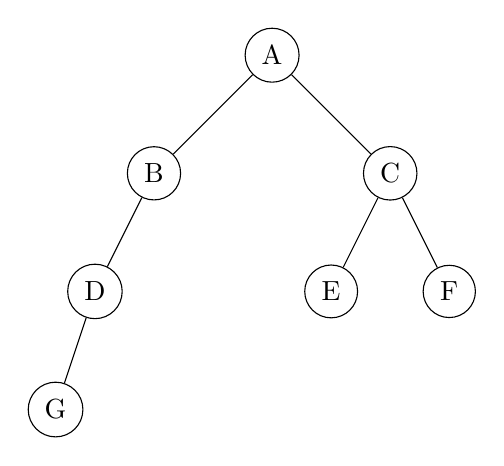
\begin{tikzpicture}[level distance=1.5cm,
level 1/.style={sibling distance=3cm},
level 2/.style={sibling distance=1.5cm},
level 3/.style={sibling distance=1cm}]

\node[circle,draw] {A}
    child {node[circle,draw] {B}
        child {node[circle,draw] {D}
            child {node[circle,draw] {G}}
            child[missing]}
        child[missing]}
    child {node[circle,draw] {C}
        child {node[circle,draw] {E}}
        child {node[circle,draw] {F}}};
\end{tikzpicture}
\end{center}

对于上述二叉树,各种遍历序列为:
\begin{itemize}
\item 前序遍历:A B D G C E F
\item 中序遍历:G D B A E C F
\item 后序遍历:G D B E F C A
\item 层序遍历:A B C D E F G
\end{itemize}

\section{二叉树的构造}

\begin{theorem}
前序遍历序列和中序遍历序列能唯一确定一棵二叉树。
\end{theorem}

\begin{example}[由遍历序列构造二叉树]
已知一棵二叉树的前序遍历序列为ABDCEF,中序遍历序列为DBAECF,构造该二叉树。

\textbf{解:}
\begin{enumerate}
\item 由前序序列可知,A是二叉树的根结点。
\item 根据中序序列,在A之前的所有结点(DB)都是A的左子树的结点,在A之后的所有结点(ECF)都是A的右子树的结点。
\item 对左子树:前序序列为BD,中序序列为DB。由前序序列知B是左子树的根结点,由中序序列知D是B的左子树结点。
\item 对右子树:前序序列为CEF,中序序列为ECF。由前序序列知C是右子树的根结点,由中序序列知E是C的左子树结点,F是C的右子树结点。
\end{enumerate}

构造过程如下:

\begin{center}
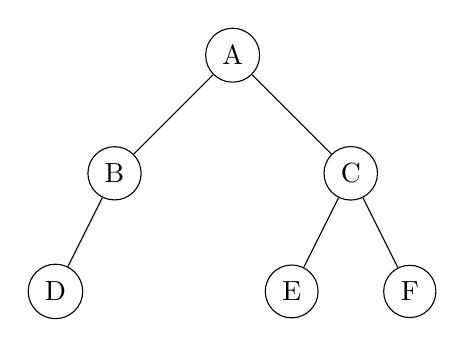
\begin{tikzpicture}[level distance=1.5cm,
level 1/.style={sibling distance=3cm},
level 2/.style={sibling distance=1.5cm}]

\node[circle,draw] {A}
    child {node[circle,draw] {B}
        child {node[circle,draw] {D}}
        child[missing]}
    child {node[circle,draw] {C}
        child {node[circle,draw] {E}}
        child {node[circle,draw] {F}}};
\end{tikzpicture}
\end{center}
\end{example}

\section{线索二叉树}

\subsection{线索二叉树的基本概念}

在具有$n$个结点的二叉链表中,共有$2n$个指针域,其中只有$n-1$个指针域用来存储孩子结点的地址,存在$n+1$个空指针域。可以利用这些空指针指向该结点在某种遍历序列中的前驱和后继结点。

\begin{definition}[线索]
指向前驱和后继结点的指针称为线索。
\end{definition}

\begin{definition}[线索二叉树]
加上线索的二叉树称为线索二叉树。
\end{definition}

\subsection{线索二叉树的结点结构}

\begin{center}
\begin{tabular}{|c|c|c|c|c|}
\hline
lchild & ltag & data & rtag & rchild \\
\hline
\end{tabular}
\end{center}

其中:
$$ltag = \begin{cases}
0 & \text{lchild指向该结点的左孩子} \\
1 & \text{lchild指向该结点的前驱}
\end{cases}$$

$$rtag = \begin{cases}
0 & \text{rchild指向该结点的右孩子} \\
1 & \text{rchild指向该结点的后继}
\end{cases}$$

\begin{lstlisting}[caption=线索二叉树结点定义]
template <typename DataType>
struct ThrNode {
    DataType data;
    int ltag, rtag;
    ThrNode<DataType> *lchild, *rchild;
};
\end{lstlisting}

\section{哈夫曼树}

\subsection{基本概念}

\begin{definition}[权值]
叶子结点的权值是对叶子结点赋予的一个有意义的数值量。
\end{definition}

\begin{definition}[带权路径长度]
设二叉树具有$n$个带权值的叶子结点,从根结点到各个叶子结点的路径长度与相应叶子结点权值的乘积之和称为二叉树的带权路径长度,记为:
$$WPL = \sum_{k=1}^{n} w_k l_k$$
其中,$w_k$为第$k$个叶子结点的权值;$l_k$为从根结点到第$k$个叶子结点的路径长度。
\end{definition}

\begin{definition}[哈夫曼树]
带权路径长度最小的二叉树称为最优二叉树,也称哈夫曼树。
\end{definition}

\subsection{哈夫曼算法}

\begin{algorithm}[H]
\caption{哈夫曼算法}
\begin{algorithmic}[1]
\REQUIRE $n$个权值$\{w_1, w_2, \ldots, w_n\}$
\ENSURE 哈夫曼树
\STATE 初始化:由$\{w_1, w_2, \ldots, w_n\}$构造$n$棵只有一个根结点的二叉树,从而得到一个二叉树集合$F = \{T_1, T_2, \ldots, T_n\}$
\WHILE{集合$F$中的二叉树个数大于1}
    \STATE 选取与合并:在$F$中选取根结点的权值最小的两棵二叉树分别作为左右子树构造一棵新的二叉树,新根结点的权值为其左右子树根结点的权值之和
    \STATE 删除与加入:在$F$中删除作为左右子树的两棵二叉树,并将新建立的二叉树加入到$F$中
\ENDWHILE
\end{algorithmic}
\end{algorithm}

\begin{example}[哈夫曼树构造]
给定权值集合$\{2, 3, 4, 5\}$,构造哈夫曼树。

\textbf{解:}

\begin{center}
\textbf{构造步骤:}

\begin{enumerate}
\item \textbf{初始状态:}四个独立结点,权值分别为2, 3, 4, 5
\item \textbf{第一步:}选择权值最小的两个结点(2和3)进行合并,生成权值为5的新结点
\item \textbf{第二步:}选择权值最小的两个结点(4和5)进行合并,生成权值为9的新结点
\item \textbf{第三步:}最后将两个子树(权值为5和9)合并,生成根结点,权值为14
\end{enumerate}

\textbf{步骤1:初始状态}

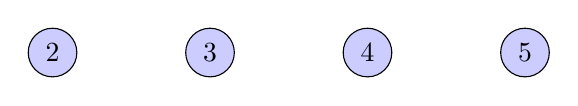
\begin{tikzpicture}
\node[circle,draw,fill=blue!20] at (0,0) {2};
\node[circle,draw,fill=blue!20] at (2,0) {3};
\node[circle,draw,fill=blue!20] at (4,0) {4};
\node[circle,draw,fill=blue!20] at (6,0) {5};
\end{tikzpicture}

\vspace{0.8cm}

\textbf{步骤2:第一次合并(2 + 3 = 5)}

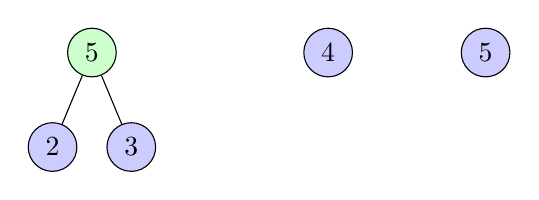
\begin{tikzpicture}[level distance=1.2cm, sibling distance=1cm]
\node[circle,draw,fill=green!20] at (1,0) {5}
    child {node[circle,draw,fill=blue!20] {2}}
    child {node[circle,draw,fill=blue!20] {3}};
\node[circle,draw,fill=blue!20] at (4,0) {4};
\node[circle,draw,fill=blue!20] at (6,0) {5};
\end{tikzpicture}

\vspace{0.8cm}

\textbf{步骤3:第二次合并(4 + 5 = 9)}

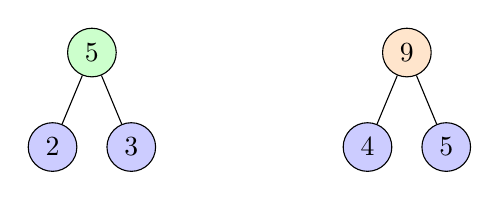
\begin{tikzpicture}[level distance=1.2cm, sibling distance=1cm]
\node[circle,draw,fill=green!20] at (1,0) {5}
    child {node[circle,draw,fill=blue!20] {2}}
    child {node[circle,draw,fill=blue!20] {3}};
\node[circle,draw,fill=orange!20] at (5,0) {9}
    child {node[circle,draw,fill=blue!20] {4}}
    child {node[circle,draw,fill=blue!20] {5}};
\end{tikzpicture}

\vspace{0.8cm}

\textbf{步骤4:最终合并(5 + 9 = 14)}

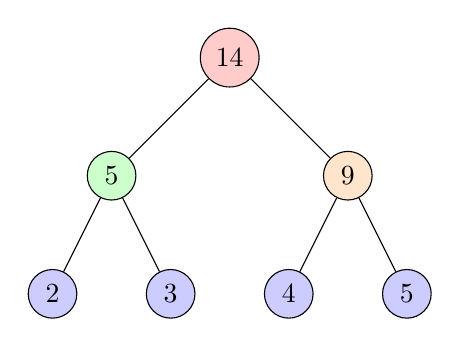
\begin{tikzpicture}[level distance=1.5cm, 
level 1/.style={sibling distance=3cm},
level 2/.style={sibling distance=1.5cm}]
\node[circle,draw,fill=red!20] {14}
    child {node[circle,draw,fill=green!20] {5}
        child {node[circle,draw,fill=blue!20] {2}}
        child {node[circle,draw,fill=blue!20] {3}}}
    child {node[circle,draw,fill=orange!20] {9}
        child {node[circle,draw,fill=blue!20] {4}}
        child {node[circle,draw,fill=blue!20] {5}}};
\end{tikzpicture}
\end{center}
该哈夫曼树的带权路径长度计算如下:

根据带权路径长度公式 $WPL = \sum_{k=1}^{n} w_k l_k$,我们需要计算每个叶子结点的权值乘以其到根结点的路径长度:

\begin{itemize}
\item 权值为2的叶子结点:从根结点到该结点需要经过3条边(根→左子树→左子树→左叶子),所以路径长度$l_1 = 3$
\item 权值为3的叶子结点:从根结点到该结点需要经过3条边(根→左子树→左子树→右叶子),所以路径长度$l_2 = 3$  
\item 权值为4的叶子结点:从根结点到该结点需要经过2条边(根→右子树→左叶子),所以路径长度$l_3 = 2$
\item 权值为5的叶子结点:从根结点到该结点需要经过2条边(根→右子树→右叶子),所以路径长度$l_4 = 2$
\end{itemize}

因此,带权路径长度为:
$$WPL = 2 \times 3 + 3 \times 3 + 4 \times 2 + 5 \times 2 = 6 + 9 + 8 + 10 = 33$$
\end{example}

\subsection{哈夫曼编码}

哈夫曼树可用于构造最短的不等长编码方案:
\begin{enumerate}
\item 以字符作为叶子结点,频率作为权值构造哈夫曼树
\item 规定左分支代表0,右分支代表1
\item 从根结点到叶子结点的路径组成该字符的编码
\end{enumerate}

\begin{example}[哈夫曼编码]
字符集$\{A, B, C, D, E\}$,使用频率分别为$\{35, 25, 15, 15, 10\}$,构造哈夫曼编码。

\textbf{构造步骤:}

\textbf{步骤1:}将所有字符按频率从小到大排列:$E(10), C(15), D(15), B(25), A(35)$

\textbf{步骤2:}选择频率最小的两个结点$E(10)$和$C(15)$合并,得到新结点权值为$10+15=25$

\textbf{步骤3:}选择频率最小的两个结点$D(15)$和新结点$(25)$合并,得到新结点权值为$15+25=40$

\textbf{步骤4:}选择频率最小的两个结点$B(25)$和$A(35)$合并,得到新结点权值为$25+35=60$

\textbf{步骤5:}最后合并剩余的两个结点$(40)$和$(60)$,得到根结点权值为$40+60=100$

\begin{center}
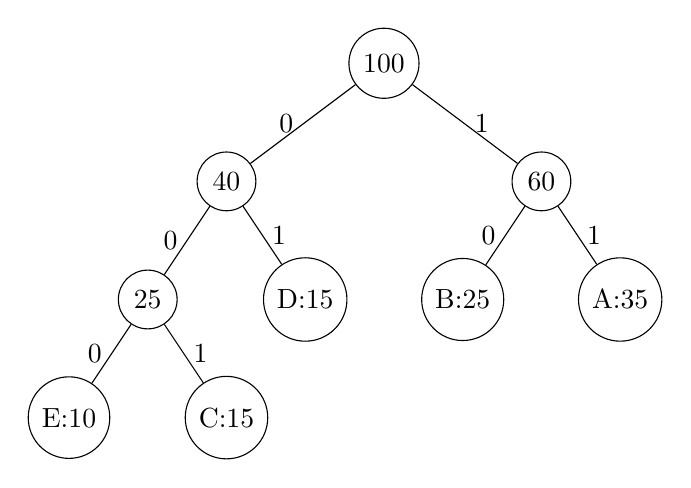
\begin{tikzpicture}[level distance=1.5cm,
level 1/.style={sibling distance=4cm},
level 2/.style={sibling distance=2cm},
level 3/.style={sibling distance=2cm}]

\node[circle,draw] {100}
    child {node[circle,draw] {40}
        child {node[circle,draw] {25}
            child {node[circle,draw] {E:10}
                edge from parent node[left] {0}}
            child {node[circle,draw] {C:15}
                edge from parent node[right] {1}}
            edge from parent node[left] {0}}
        child {node[circle,draw] {D:15}
            edge from parent node[right] {1}}
        edge from parent node[left] {0}}
    child {node[circle,draw] {60}
        child {node[circle,draw] {B:25}
            edge from parent node[left] {0}}
        child {node[circle,draw] {A:35}
            edge from parent node[right] {1}}
        edge from parent node[right] {1}};
\end{tikzpicture}
\end{center}

\textbf{编码方法:}
\begin{enumerate}
\item 规定左分支代表0,右分支代表1
\item 从根结点到每个叶子结点的路径组成该字符的编码
\item 具体编码过程:
\begin{itemize}
\item 字符A:根→右→右,编码为11
\item 字符B:根→右→左,编码为10
\item 字符C:根→左→左→右,编码为001
\item 字符D:根→左→右,编码为01
\item 字符E:根→左→左→左,编码为000
\end{itemize}
\end{enumerate}

编码结果:
\begin{center}
\begin{tabular}{|c|c|c|c|}
\hline
字符 & 频率 & 编码 & 编码长度 \\
\hline
A & 35 & 11 & 2 \\
B & 25 & 10 & 2 \\
C & 15 & 001 & 3 \\
D & 15 & 01 & 2 \\
E & 10 & 000 & 3 \\
\hline
\end{tabular}
\end{center}

\textbf{编码特点:}
\begin{itemize}
\item 频率高的字符使用较短的编码(A、B、D使用2位编码)
\item 频率低的字符使用较长的编码(C、E使用3位编码)
\item 任何字符的编码都不是另一个字符编码的前缀(前缀码性质)
\end{itemize}
\end{example}

\section{堆与优先队列}

\subsection{堆的定义与性质}

\begin{definition}[堆]
堆是具有下列性质的完全二叉树:
\begin{itemize}
\item \textbf{大根堆(最大堆)}:每个结点的值都大于或等于其左右孩子结点的值
\item \textbf{小根堆(最小堆)}:每个结点的值都小于或等于其左右孩子结点的值
\end{itemize}
\end{definition}

\textbf{堆的重要性质:}
\begin{enumerate}
\item 堆是完全二叉树,可以用数组存储,节省空间
\item 如果将堆按层序从1开始编号,则结点之间满足如下关系:
$$\text{大根堆:}\begin{cases}
k_i \geq k_{2i} \\
k_i \geq k_{2i+1}
\end{cases} \quad \text{小根堆:}\begin{cases}
k_i \leq k_{2i} \\
k_i \leq k_{2i+1}
\end{cases} \quad (1 \leq i \leq \lfloor n/2 \rfloor)$$
\item 对于编号为$i$的结点:
\begin{itemize}
\item 父结点编号:$\lfloor i/2 \rfloor$
\item 左孩子编号:$2i$
\item 右孩子编号:$2i+1$
\end{itemize}
\end{enumerate}

\textbf{堆的示例:}
\begin{center}
\begin{tikzpicture}[level distance=1.5cm,
level 1/.style={sibling distance=3cm},
level 2/.style={sibling distance=1.5cm},
level 3/.style={sibling distance=1cm}]

\node[circle,draw] {90}
    child {node[circle,draw] {80}
        child {node[circle,draw] {65}}
        child {node[circle,draw] {70}}}
    child {node[circle,draw] {85}
        child {node[circle,draw] {60}}
        child {node[circle,draw] {75}}};

\node at (0,-4) {\textbf{大根堆示例}};
\end{tikzpicture}
\quad
\begin{tikzpicture}[level distance=1.5cm,
level 1/.style={sibling distance=3cm},
level 2/.style={sibling distance=1.5cm},
level 3/.style={sibling distance=1cm}]

\node[circle,draw] {10}
    child {node[circle,draw] {20}
        child {node[circle,draw] {35}}
        child {node[circle,draw] {30}}}
    child {node[circle,draw] {15}
        child {node[circle,draw] {40}}
        child {node[circle,draw] {25}}};

\node at (0,-4) {\textbf{小根堆示例}};
\end{tikzpicture}
\end{center}

\subsection{堆的基本操作}

\subsubsection{堆的插入操作(向上调整)}

\textbf{算法思想:}
\begin{enumerate}
\item 将新元素插入到堆的末尾(保持完全二叉树性质)
\item 将新元素与其父结点比较,如果违反堆的性质则交换
\item 重复步骤2,直到满足堆的性质或到达根结点
\end{enumerate}

\begin{algorithm}[H]
\caption{堆的插入操作(大根堆)}
\begin{algorithmic}[1]
\REQUIRE 待插入元素$x$,堆数组$heap[]$,堆大小$size$
\ENSURE 维护堆的性质
\STATE $size \leftarrow size + 1$
\STATE $heap[size] \leftarrow x$
\STATE $i \leftarrow size$
\WHILE{$i > 1$ 且 $heap[i] > heap[i/2]$}
    \STATE 交换$heap[i]$和$heap[i/2]$
    \STATE $i \leftarrow i/2$
\ENDWHILE
\end{algorithmic}
\end{algorithm}

\begin{lstlisting}[caption=堆插入操作的C++实现]
void insertHeap(vector<int>& heap, int x) {
    heap.push_back(x);
    int i = heap.size() - 1;
    
    // 向上调整
    while (i > 0 && heap[i] > heap[(i-1)/2]) {
        swap(heap[i], heap[(i-1)/2]);
        i = (i-1)/2;
    }
}
\end{lstlisting}

\subsubsection{堆的删除操作(向下调整)}

\textbf{算法思想:}
\begin{enumerate}
\item 保存堆顶元素(要删除的元素)
\item 将堆的最后一个元素移到堆顶
\item 从堆顶开始向下调整,与较大的孩子交换(大根堆)
\item 重复调整直到满足堆的性质
\end{enumerate}

\begin{algorithm}[H]
\caption{堆的删除操作(大根堆)}
\begin{algorithmic}[1]
\REQUIRE 堆数组$heap[]$,堆大小$size$
\ENSURE 删除堆顶元素并维护堆的性质
\STATE $result \leftarrow heap[1]$
\STATE $heap[1] \leftarrow heap[size]$
\STATE $size \leftarrow size - 1$
\STATE $i \leftarrow 1$
\WHILE{$2i \leq size$}
    \STATE $j \leftarrow 2i$ \COMMENT{左孩子}
    \IF{$j < size$ 且 $heap[j] < heap[j+1]$}
        \STATE $j \leftarrow j+1$ \COMMENT{选择较大的孩子}
    \ENDIF
    \IF{$heap[i] \geq heap[j]$}
        \STATE \textbf{break} \COMMENT{已满足堆性质}
    \ELSE
        \STATE 交换$heap[i]$和$heap[j]$
        \STATE $i \leftarrow j$
    \ENDIF
\ENDWHILE
\RETURN $result$
\end{algorithmic}
\end{algorithm}

\subsubsection{建堆操作}

\textbf{方法一:逐个插入法}
\begin{itemize}
\item 从空堆开始,逐个插入元素
\item 时间复杂度:$O(n \log n)$
\end{itemize}

\textbf{方法二:自底向上调整法(更高效)}
\begin{itemize}
\item 将数组看作完全二叉树
\item 从最后一个非叶子结点开始,向前逐个进行向下调整
\item 时间复杂度:$O(n)$
\end{itemize}

\begin{algorithm}[H]
\caption{建堆操作(自底向上)}
\begin{algorithmic}[1]
\REQUIRE 数组$A[1..n]$
\ENSURE 将数组调整为大根堆
\FOR{$i = \lfloor n/2 \rfloor$ \textbf{downto} $1$}
    \STATE 对以$A[i]$为根的子树进行向下调整
\ENDFOR
\end{algorithmic}
\end{algorithm}

\subsection{堆排序}

\textbf{基本思想:}
\begin{enumerate}
\item 将待排序数组建成大根堆
\item 将堆顶元素(最大值)与堆的最后一个元素交换
\item 堆大小减1,对新的堆顶进行向下调整
\item 重复步骤2-3,直到堆大小为1
\end{enumerate}

\begin{lstlisting}[caption=堆排序算法实现]
void heapSort(vector<int>& arr) {
    int n = arr.size();
    
    // 建堆
    for (int i = n/2 - 1; i >= 0; i--) {
        heapify(arr, n, i);
    }
    
    // 排序
    for (int i = n-1; i > 0; i--) {
        swap(arr[0], arr[i]);  // 将最大元素放到末尾
        heapify(arr, i, 0);    // 调整剩余元素
    }
}

void heapify(vector<int>& arr, int n, int i) {
    int largest = i;
    int left = 2*i + 1;
    int right = 2*i + 2;
    
    if (left < n && arr[left] > arr[largest])
        largest = left;
    if (right < n && arr[right] > arr[largest])
        largest = right;
        
    if (largest != i) {
        swap(arr[i], arr[largest]);
        heapify(arr, n, largest);
    }
}
\end{lstlisting}

\textbf{堆排序的特点:}
\begin{itemize}
\item 时间复杂度:$O(n \log n)$(最好、平均、最坏情况都相同)
\item 空间复杂度:$O(1)$(原地排序)
\item 不稳定排序
\item 适合处理大数据量的排序问题
\end{itemize}

\subsection{优先队列}

\begin{definition}[优先队列]
优先队列是一种抽象数据类型,支持以下操作:
\begin{itemize}
\item 插入元素(insert)
\item 删除并返回优先级最高的元素(deleteMax/deleteMin)
\item 查看优先级最高的元素(top/peek)
\end{itemize}
\end{definition}

\textbf{优先队列的实现方式比较:}
\begin{center}
\begin{tabular}{|l|c|c|c|}
\hline
\textbf{实现方式} & \textbf{插入} & \textbf{删除最值} & \textbf{查找最值} \\
\hline
无序数组 & $O(1)$ & $O(n)$ & $O(n)$ \\
\hline
有序数组 & $O(n)$ & $O(1)$ & $O(1)$ \\
\hline
无序链表 & $O(1)$ & $O(n)$ & $O(n)$ \\
\hline
有序链表 & $O(n)$ & $O(1)$ & $O(1)$ \\
\hline
二叉堆 & $O(\log n)$ & $O(\log n)$ & $O(1)$ \\
\hline
\end{tabular}
\end{center}

\textbf{应用实例:}
\begin{enumerate}
\item \textbf{任务调度}:操作系统中根据优先级调度进程
\item \textbf{哈夫曼编码}:构造哈夫曼树时需要反复取出频率最小的结点
\item \textbf{图算法}:Dijkstra最短路径算法、Prim最小生成树算法
\item \textbf{事件模拟}:按时间顺序处理事件
\end{enumerate}

\begin{example}[堆操作过程演示]
对序列$(10, 20, 15, 30, 40)$建立大根堆,然后依次删除堆顶元素。

\textbf{建堆过程:}
\begin{enumerate}
\item 初始数组:$[10, 20, 15, 30, 40]$
\item 从最后一个非叶子结点开始调整($i = \lfloor 5/2 \rfloor = 2$)
\item 调整结点2(值为15):与孩子40比较,交换得到$[10, 20, 40, 30, 15]$
\item 调整结点1(值为20):与孩子30比较,交换得到$[10, 30, 40, 20, 15]$
\item 调整结点0(值为10):与孩子40比较,交换得到$[40, 30, 10, 20, 15]$
\item 继续调整:10与20比较,交换得到$[40, 30, 20, 10, 15]$
\end{enumerate}

\textbf{删除过程:}
\begin{enumerate}
\item 删除40:将15移到堆顶,调整得到$[30, 15, 20, 10]$
\item 删除30:将10移到堆顶,调整得到$[20, 15, 10]$
\item 删除20:将10移到堆顶,调整得到$[15, 10]$
\item 删除15:得到$[10]$
\item 删除10:堆为空
\end{enumerate}
\end{example}

\section{二叉树的应用}

\subsection{表达式树}

二叉表达式树是对应一个算术表达式的二叉树,具有以下特点:
\begin{enumerate}
\item 叶子结点一定是操作数
\item 分支结点一定是运算符
\end{enumerate}

\begin{example}[构造表达式树]
将表达式$(A+B) \times (C+D \times E)$转换为二叉表达式树。

\begin{center}
\begin{tikzpicture}[level distance=1.5cm,
level 1/.style={sibling distance=4cm},
level 2/.style={sibling distance=2cm},
level 3/.style={sibling distance=1cm}]

\node[circle,draw] {$\times$}
    child {node[circle,draw] {$+$}
        child {node[circle,draw] {A}}
        child {node[circle,draw] {B}}}
    child {node[circle,draw] {$+$}
        child {node[circle,draw] {C}}
        child {node[circle,draw] {$\times$}
            child {node[circle,draw] {D}}
            child {node[circle,draw] {E}}}};
\end{tikzpicture}
\end{center}

遍历结果:
\begin{itemize}
\item 前序遍历:$\times + A B + C \times D E$(前缀表达式)
\item 中序遍历:$A + B \times C + D \times E$(中缀表达式)
\item 后序遍历:$A B + C D E \times + \times$(后缀表达式)
\end{itemize}
\end{example}

\section{常见考点总结}

\subsection{重点掌握内容}

\begin{enumerate}
\item \textbf{二叉树的基本性质}:特别是性质1($n_0 = n_2 + 1$)和性质5(完全二叉树的编号关系)
\item \textbf{二叉树的遍历}:四种遍历方法的递归和非递归实现
\item \textbf{由遍历序列构造二叉树}:前序+中序或后序+中序唯一确定二叉树
\item \textbf{哈夫曼树的构造和编码}:算法过程和编码方法
\item \textbf{线索二叉树}:线索化过程和在线索二叉树上的遍历
\item \textbf{堆的基本操作}:插入和删除操作的调整过程
\end{enumerate}

\subsection{常见题型}

\begin{enumerate}
\item 根据二叉树的性质计算结点个数、深度等
\item 写出给定二叉树的各种遍历序列
\item 根据遍历序列构造二叉树
\item 设计二叉树遍历的递归和非递归算法
\item 哈夫曼树的构造和编码设计
\item 完全二叉树的性质和应用
\item 线索二叉树的构造和遍历
\end{enumerate}

\subsection{重要算法复杂度}

\begin{center}
\begin{tabular}{|l|c|c|}
\hline
\textbf{操作} & \textbf{时间复杂度} & \textbf{空间复杂度} \\
\hline
二叉树遍历(递归) & $O(n)$ & $O(h)$ \\
二叉树遍历(非递归) & $O(n)$ & $O(h)$ \\
哈夫曼树构造 & $O(n\log n)$ & $O(n)$ \\
堆的插入 & $O(\log n)$ & $O(1)$ \\
堆的删除 & $O(\log n)$ & $O(1)$ \\
线索化 & $O(n)$ & $O(h)$ \\
\hline
\end{tabular}
\end{center}

\section{典型例题解析}

\begin{example}[结点个数计算]
一棵完全二叉树有780个结点,其中叶子结点的个数是多少?

\textbf{解:}
设度为0、1、2的结点个数分别为$n_0$、$n_1$、$n_2$。

由二叉树性质1:$n_0 = n_2 + 1$

总结点数:$n_0 + n_1 + n_2 = 780$

对于完全二叉树,$n_1 \leq 1$(最多只有一个度为1的结点)

代入得:$(n_2 + 1) + n_1 + n_2 = 780$

即:$2n_2 + n_1 + 1 = 780$

所以:$2n_2 + n_1 = 779$

由于$n_1 \leq 1$,当$n_1 = 1$时,$n_2 = 389$,$n_0 = 390$
当$n_1 = 0$时,$n_2 = 389.5$(不是整数,不合理)

因此,叶子结点个数为390。
\end{example}

\begin{example}[遍历序列应用]
已知二叉树的前序遍历序列为ABDHECFIG,中序遍历序列为HDBECAIFG,画出该二叉树。

\textbf{解:}
\begin{enumerate}
\item 由前序序列知A是根结点
\item 由中序序列知,A左边的HDBEC是左子树,A右边的IFG是右子树
\item 递归处理左子树:前序为BDHEC,中序为HDBEC
\item 递归处理右子树:前序为FIG,中序为IFG
\end{enumerate}

最终构造的二叉树如下:

\begin{center}
\begin{tikzpicture}[level distance=1.5cm,
level 1/.style={sibling distance=5cm},
level 2/.style={sibling distance=2.5cm},
level 3/.style={sibling distance=1.5cm}]

\node[circle,draw] {A}
    child {node[circle,draw] {B}
        child {node[circle,draw] {D}
            child {node[circle,draw] {H}}
            child[missing]}
        child {node[circle,draw] {E}
            child[missing]
            child {node[circle,draw] {C}}}}
    child {node[circle,draw] {F}
        child {node[circle,draw] {I}}
        child {node[circle,draw] {G}}};
\end{tikzpicture}
\end{center}
\end{example}

\section{复习建议}

\subsection{学习方法}

\begin{enumerate}
\item \textbf{理解概念}:深入理解二叉树的定义和性质,特别是与普通树的区别
\item \textbf{掌握算法}:熟练掌握各种遍历算法的递归和非递归实现
\item \textbf{练习构造}:通过遍历序列构造二叉树的方法要反复练习
\item \textbf{应用实践}:理解二叉树在实际问题中的应用,如表达式树、哈夫曼编码等
\item \textbf{代码实现}:能够用代码实现二叉树的基本操作
\end{enumerate}

\subsection{复习重点}

\begin{enumerate}
\item 二叉树的五个基本性质及其证明和应用
\item 四种遍历方法的定义、实现和应用
\item 线索二叉树的构造和遍历
\item 哈夫曼树的构造算法和编码方法
\item 堆的定义、性质和基本操作
\item 完全二叉树的性质和应用
\end{enumerate}

\subsection{常见错误}

\begin{enumerate}
\item 混淆二叉树和度为2的树的概念
\item 遍历算法的递归出口条件错误
\item 完全二叉树性质应用错误
\item 哈夫曼编码的构造过程错误
\item 线索二叉树的线索方向搞错
\end{enumerate}

\end{document}
% \documentclass[12pt,a4paper]{amsart}
\usepackage[utf8]{inputenc}
\usepackage[T1]{fontenc}
\usepackage{amsmath,amsfonts,amssymb}
\usepackage{tikz}
\usepackage{algorithm}
\usepackage{algorithmic}
\usepackage{listings}
\usepackage{xcolor}
\usepackage{geometry}
\usepackage{fancyhdr}
\usepackage{enumitem}
\usepackage{booktabs}
\usepackage{multirow}
\usepackage[hidelinks,bookmarksnumbered,bookmarksopen]{hyperref}
\usepackage{xeCJK}
\setCJKmainfont{LXGW WenKai}


% 页面设置
\geometry{left=2cm,right=2cm,top=2.5cm,bottom=2.5cm}
\pagestyle{fancy}
\fancyhf{}
\fancyhead[L]{图论复习总结}
\fancyhead[R]{\thepage}

% TikZ库
\usetikzlibrary{arrows,positioning,shapes,calc,trees,graphs}

% 代码高亮设置
\lstset{
    language=C++,
    basicstyle=\ttfamily\small,
    keywordstyle=\color{blue}\bfseries,
    commentstyle=\color{green!60!black},
    stringstyle=\color{red},
    numbers=left,
    numberstyle=\tiny\color{gray},
    stepnumber=1,
    numbersep=10pt,
    backgroundcolor=\color{gray!10},
    frame=single,
    tabsize=4,
    captionpos=b,
    breaklines=true,
    breakatwhitespace=false,
    showspaces=false,
    showstringspaces=false,
    showtabs=false
}

% 定理环境
\newtheorem{definition}{定义}[section]
\newtheorem{theorem}{定理}[section]
\newtheorem{algorithm_desc}{算法}[section]

\title{\textbf{数据结构第六章:图论复习总结}}
\author{期末考试复习资料}
\date{\today}

\begin{document}

% \maketitle

% % 目录设置
% \tableofcontents
% \newpage

\section{图的基本概念}

\subsection{图的定义}

\begin{definition}[图]
图是由顶点的有穷非空集合和顶点之间边的集合组成,通常表示为:
$$G = (V, E)$$
其中$G$表示一个图,$V$是顶点集合,$E$是边集合。
\end{definition}

\begin{center}
\begin{tikzpicture}[scale=1.2]
    % 无向图示例
    \node[circle,draw,minimum size=0.8cm] (v0) at (0,0) {$v_0$};
    \node[circle,draw,minimum size=0.8cm] (v1) at (2,1) {$v_1$};
    \node[circle,draw,minimum size=0.8cm] (v2) at (2,-1) {$v_2$};
    \node[circle,draw,minimum size=0.8cm] (v3) at (4,0) {$v_3$};
    
    \draw (v0) -- (v1);
    \draw (v0) -- (v2);
    \draw (v1) -- (v3);
    \draw (v2) -- (v3);
    \draw (v1) -- (v2);
    
    \node at (2,-2) {\textbf{无向图}};
    
    % 有向图示例
    \begin{scope}[xshift=6cm]
        \node[circle,draw,minimum size=0.8cm] (u0) at (0,0) {$u_0$};
        \node[circle,draw,minimum size=0.8cm] (u1) at (2,1) {$u_1$};
        \node[circle,draw,minimum size=0.8cm] (u2) at (2,-1) {$u_2$};
        \node[circle,draw,minimum size=0.8cm] (u3) at (4,0) {$u_3$};
        
        \draw[-latex] (u0) -- (u1);
        \draw[-latex] (u0) -- (u2);
        \draw[-latex] (u1) -- (u3);
        \draw[-latex] (u2) -- (u3);
        \draw[-latex,bend left] (u1) to (u2);
        
        \node at (2,-2) {\textbf{有向图}};
    \end{scope}
\end{tikzpicture}
\end{center}

\subsection{图的基本术语}

\begin{itemize}
    \item \textbf{邻接}:若存在边$(v_i, v_j)$,则称$v_i$和$v_j$互为邻接点
    \item \textbf{关联(依附)}:顶点$v$和边$e$相关联,称边$e$依附于顶点$v$
    \item \textbf{度}:
    \begin{itemize}
        \item 无向图:顶点$v$的度$TD(v)$是依附于该顶点的边数
        \item 有向图:入度$ID(v)$ + 出度$OD(v)$
        \item 悬挂顶点:度为1的顶点
        \item 孤立顶点:度为0的顶点
    \end{itemize}
    \item \textbf{路径与回路}:
    \begin{itemize}
        \item 路径:顶点序列$v_p = v_{i_0}v_{i_1}\cdots v_{i_m} = v_q$
        \item 路径长度:路径上边的数目
        \item 简单路径:顶点不重复的路径
        \item 回路(环):第一个和最后一个顶点相同的路径
        \item 简单回路:除第一个和最后一个顶点外,其余顶点不重复的回路
    \end{itemize}
    \item \textbf{连通性}:
    \begin{itemize}
        \item 连通:任意两顶点间都有路径的无向图
        \item 连通分量:无向图中的极大连通子图
        \item 强连通:任意两顶点间都有路径的有向图
        \item 强连通分量:有向图中的极大强连通子图
    \end{itemize}
    \item \textbf{特殊图类型}:
    \begin{itemize}
        \item 完全图:任意两个顶点之间都有边的简单图
        \item 无向完全图:$n$个顶点的完全图有$\frac{n(n-1)}{2}$条边
        \item 有向完全图:$n$个顶点的完全图有$n(n-1)$条弧
        \item 树:$n$个顶点$n-1$条边的连通无向图
        \item 森林:若干棵不相交树的集合
    \end{itemize}
\end{itemize}

\subsection{重要数学性质}

\begin{theorem}[握手定理]
在具有$n$个顶点$e$条边的无向图中:
$$\sum_{i=0}^{n-1} TD(v_i) = 2e$$
\end{theorem}

\begin{theorem}[有向图度数性质]
在具有$n$个顶点$e$条边的有向图中:
$$\sum_{i=0}^{n-1} ID(v_i) = \sum_{i=0}^{n-1} OD(v_i) = e$$
\end{theorem}

\section{图的存储结构}

\subsection{邻接矩阵}

\begin{definition}[邻接矩阵]
用$n \times n$的二维数组存储图,其中$A[i][j] = 1$表示存在边$(v_i, v_j)$。
\end{definition}

\begin{center}
\begin{tikzpicture}[scale=1]
    % 图示例
    \node[circle,draw,minimum size=0.6cm] (v0) at (0,2) {0};
    \node[circle,draw,minimum size=0.6cm] (v1) at (2,2) {1};
    \node[circle,draw,minimum size=0.6cm] (v2) at (0,0) {2};
    \node[circle,draw,minimum size=0.6cm] (v3) at (2,0) {3};
    
    \draw (v0) -- (v1);
    \draw (v0) -- (v2);
    \draw (v1) -- (v3);
    \draw (v2) -- (v3);
    \draw (v1) -- (v2);
    
    % 邻接矩阵
    \begin{scope}[xshift=5cm, yshift=0.5cm]
        \draw (0,0) grid (4,4);
        \foreach \i in {0,1,2,3} {
            \node at (-0.5,3.5-\i) {\i};
            \node at (\i+0.5,4.5) {\i};
        }
        
        % 填入数值 - 修正为正确的邻接矩阵
        \node at (0.5,3.5) {0}; \node at (1.5,3.5) {1}; \node at (2.5,3.5) {1}; \node at (3.5,3.5) {0};
        \node at (0.5,2.5) {1}; \node at (1.5,2.5) {0}; \node at (2.5,2.5) {1}; \node at (3.5,2.5) {1};
        \node at (0.5,1.5) {1}; \node at (1.5,1.5) {1}; \node at (2.5,1.5) {0}; \node at (3.5,1.5) {1};
        \node at (0.5,0.5) {0}; \node at (1.5,0.5) {1}; \node at (2.5,0.5) {1}; \node at (3.5,0.5) {0};
        
        \node at (2,-1) {\textbf{邻接矩阵}};
    \end{scope}
\end{tikzpicture}
\end{center}

\begin{lstlisting}[caption=邻接矩阵类定义]
template<typename DataType>
class MGraph {
private:
    DataType vertex[MaxSize];           // 顶点数组
    int edge[MaxSize][MaxSize];         // 邻接矩阵
    int vertexNum, edgeNum;             // 顶点数和边数

public:
    MGraph(DataType a[], int n, int e); // 构造函数
    ~MGraph();                          // 析构函数
    void DFTraverse(int v);             // 深度优先遍历
    void BFTraverse(int v);             // 广度优先遍历
};
\end{lstlisting}

\subsection{邻接表}

\begin{definition}[邻接表]
由顶点表和边表组成,顶点表存储顶点信息,边表用链表存储该顶点的所有邻接点。
\end{definition}

\begin{center}
\begin{tikzpicture}[scale=1]
    % 定义样式
    \tikzset{
        vertexbox/.style={draw,fill=blue!10,minimum width=0.8cm,minimum height=0.6cm,font=\large\bfseries},
        edgebox/.style={draw,fill=green!10,minimum width=0.6cm,minimum height=0.5cm,font=\footnotesize},
        arrow/.style={->,thick,color=blue!70}
    }
    
    % 顶点表标题
    \node[font=\large\bfseries] at (0.5,4.8) {顶点表};
    \node[font=\large\bfseries] at (4,4.8) {邻接点链表};
    
    % 顶点表
    \foreach \i in {0,1,2,3} {
        \node[vertexbox] (v\i) at (0.5,3.5-\i) {\i};
        \draw[arrow] (v\i.east) -- ++(0.7,0);
    }
    
    % 边表 - 顶点0:连接1,2
    \node[edgebox] (e0-1) at (2.2,3.5) {1};
    \node[edgebox] (e0-2) at (3.2,3.5) {2};
    \node[font=\small] (null0) at (4.5,3.5) {NULL};
    \draw[arrow] (e0-1.east) -- (e0-2.west);
    \draw[arrow] (e0-2.east) -- (null0.west);
    
    % 边表 - 顶点1:连接0,2,3
    \node[edgebox] (e1-0) at (2.2,2.5) {0};
    \node[edgebox] (e1-2) at (3.2,2.5) {2};
    \node[edgebox] (e1-3) at (4.2,2.5) {3};
    \node[font=\small] (null1) at (5.5,2.5) {NULL};
    \draw[arrow] (e1-0.east) -- (e1-2.west);
    \draw[arrow] (e1-2.east) -- (e1-3.west);
    \draw[arrow] (e1-3.east) -- (null1.west);
    
    % 边表 - 顶点2:连接0,1,3
    \node[edgebox] (e2-0) at (2.2,1.5) {0};
    \node[edgebox] (e2-1) at (3.2,1.5) {1};
    \node[edgebox] (e2-3) at (4.2,1.5) {3};
    \node[font=\small] (null2) at (5.5,1.5) {NULL};
    \draw[arrow] (e2-0.east) -- (e2-1.west);
    \draw[arrow] (e2-1.east) -- (e2-3.west);
    \draw[arrow] (e2-3.east) -- (null2.west);
    
    % 边表 - 顶点3:连接1,2
    \node[edgebox] (e3-1) at (2.2,0.5) {1};
    \node[edgebox] (e3-2) at (3.2,0.5) {2};
    \node[font=\small] (null3) at (4.5,0.5) {NULL};
    \draw[arrow] (e3-1.east) -- (e3-2.west);
    \draw[arrow] (e3-2.east) -- (null3.west);
    
    % 添加分隔线
    \draw[dashed,gray] (1.5,4) -- (1.5,-0.2);
    
    % 底部标题
    \node[font=\large\bfseries] at (2.5,-0.8) {邻接表存储结构示例};
\end{tikzpicture}
\end{center}

\begin{lstlisting}[caption=邻接表结构定义]
// 边表结点
struct EdgeNode {
    int adjvex;                         // 邻接点编号
    EdgeNode* next;                     // 指向下一个边结点
};

// 顶点表结点
template<typename DataType>
struct VertexNode {
    DataType vertex;                    // 顶点数据
    EdgeNode* firstEdge;               // 指向第一条边的指针
};

template<typename DataType>
class ALGraph {
private:
    VertexNode<DataType> adjlist[MaxSize]; // 顶点表数组
    int vertexNum, edgeNum;                // 顶点数和边数
    
public:
    ALGraph(DataType a[], int n, int e);
    ~ALGraph();
    void DFTraverse(int v);
    void BFTraverse(int v);
};
\end{lstlisting}

\subsection{存储结构比较}

\begin{table}[h]
\centering
\begin{tabular}{lcc}
\toprule
\textbf{比较项目} & \textbf{邻接矩阵} & \textbf{邻接表} \\
\midrule
空间复杂度 & $O(n^2)$ & $O(n+e)$ \\
判断是否邻接 & $O(1)$ & $O(d)$ \\
找所有邻接点 & $O(n)$ & $O(d)$ \\
适用图类型 & 稠密图 & 稀疏图 \\
表示唯一性 & 唯一 & 不唯一 \\
\bottomrule
\end{tabular}
\caption{邻接矩阵与邻接表比较}
\end{table}

\textbf{符号说明}:
\begin{itemize}
    \item $n$:图中顶点的数量
    \item $e$:图中边的数量
    \item $d$:顶点的度数(degree),即与该顶点相邻的边的数量
\end{itemize}

\section{图的遍历}

\subsection{深度优先遍历(DFS)}

\begin{algorithm}[H]
\caption{深度优先遍历}
\begin{algorithmic}[1]
\STATE 深度优先遍历类似于树的前序遍历。从图中某顶点$v$出发进行深度优先遍历的基本思想是:
\STATE 1. 访问顶点$v$
\STATE 2. 从$v$的未被访问的邻接点中选取一个顶点$w$,然后从$w$出发进行深度优先遍历
\STATE 3. 重复上述两步,直至图中所有和$v$有路径相通的顶点都被访问到
\STATE 显然,深度优先遍历图是一个递归过程。
\end{algorithmic}
\end{algorithm}

\textbf{算法伪代码描述}:
\begin{verbatim}
算法: DFTraverse
输入: 顶点的编号 v
输出: 无
1. 访问顶点v; 修改标志 visited[v]=1;
2. w = 第一个未被访问的邻接点;
3. while (w存在) do
   3.1 DFTraverse(w);
   3.2 w = 下一个未被访问的邻接点;
\end{verbatim}

\begin{center}
\begin{tikzpicture}[scale=1]
    % DFS遍历示例
    \node[circle,draw,fill=red!20,minimum size=0.8cm] (v0) at (0,0) {0};
    \node[circle,draw,fill=yellow!20,minimum size=0.8cm] (v1) at (2,1) {1};
    \node[circle,draw,fill=green!20,minimum size=0.8cm] (v2) at (2,-1) {2};
    \node[circle,draw,fill=blue!20,minimum size=0.8cm] (v3) at (4,1) {3};
    \node[circle,draw,fill=purple!20,minimum size=0.8cm] (v4) at (4,-1) {4};
    
    \draw[thick] (v0) -- (v1);
    \draw (v0) -- (v2);
    \draw[thick] (v1) -- (v3);
    \draw[thick] (v1) -- (v4);
    \draw (v2) -- (v4);
    
    % 遍历顺序标注
    \node at (0,-0.7) {\small 1};
    \node at (2,1.7) {\small 2};
    \node at (4,1.7) {\small 3};
    \node at (4,-1.7) {\small 4};
    \node at (2,-1.7) {\small 5};
    
    \node at (2,-2.5) {\textbf{DFS访问序列: 0→1→3→4→2}};
\end{tikzpicture}
\end{center}

\textbf{邻接矩阵实现}:
\begin{lstlisting}[caption=邻接矩阵的深度优先遍历]
template <typename DataType>
void MGraph<DataType>::DFTraverse(int v)
{
    cout <<vertex[v]; visited[v] = 1;
    for (int j = 0; j < vertexNum; j++)
        if (edge[v][j] == 1 && visited[j] == 0) DFTraverse(j);
}
\end{lstlisting}

\textbf{邻接表实现}:
\begin{lstlisting}[caption=邻接表的深度优先遍历]
template <typename DataType>
void ALGraph<DataType>::DFTraverse(int v)
{
    int j;
    EdgeNode * p = nullptr;
    cout <<adjlist[v].vertex; visited[v] = 1;
    p = adjlist[v].firstEdge; //工作指针p指向顶点v的边表
    while(p != nullptr) //依次搜索顶点v的邻接点j
    {
        j = p->adjvex;
        if(visited[j] == 0) DFTraverse(j);
        p = p->next;
    }
}
\end{lstlisting}

\textbf{时间复杂度分析}:
\begin{itemize}
    \item 邻接矩阵存储:时间复杂度为$O(n^2)$,其中$n$为图中顶点个数
    \item 邻接表存储:时间复杂度为$O(n+e)$,其中$n$为顶点个数,$e$为边数
\end{itemize}

\subsection{广度优先遍历(BFS)}

\begin{algorithm}[H]
\caption{广度优先遍历}
\begin{algorithmic}[1]
\STATE 广度优先遍历类似于树的层序遍历。从图中某顶点$v$出发进行广度优先遍历的基本思想是:
\STATE 1. 访问顶点$v$
\STATE 2. 依次访问$v$的各个未被访问的邻接点
\STATE 3. 分别从这些邻接点出发,依次访问它们的未被访问的邻接点
\STATE 4. 重复上述过程,直到所有和$v$有路径相通的顶点都被访问到
\end{algorithmic}
\end{algorithm}

\textbf{算法伪代码描述}:
\begin{verbatim}
算法: BFTraverse
输入: 顶点的编号 v
输出: 无
1. 访问顶点v; 修改标志 visited[v]=1; 顶点v入队;
2. while (队列非空) do
   2.1 队头顶点u出队;
   2.2 w = u的第一个未被访问的邻接点;
   2.3 while (w存在) do
       2.3.1 访问顶点w; 修改标志 visited[w]=1; 顶点w入队;
       2.3.2 w = u的下一个未被访问的邻接点;
\end{verbatim}

\begin{center}
\begin{tikzpicture}[scale=1]
    % BFS遍历示例
    \node[circle,draw,fill=red!20,minimum size=0.8cm] (v0) at (2,2) {0};
    \node[circle,draw,fill=yellow!20,minimum size=0.8cm] (v1) at (0,0) {1};
    \node[circle,draw,fill=yellow!20,minimum size=0.8cm] (v2) at (2,0) {2};
    \node[circle,draw,fill=yellow!20,minimum size=0.8cm] (v3) at (4,0) {3};
    \node[circle,draw,fill=green!20,minimum size=0.8cm] (v4) at (1,-1) {4};
    
    \draw (v0) -- (v1);
    \draw (v0) -- (v2);
    \draw (v0) -- (v3);
    \draw (v1) -- (v4);
    \draw (v2) -- (v4);
    
    % 层次标注
    \draw[dashed] (-0.5,1.5) -- (4.5,1.5);
    \draw[dashed] (-0.5,-0.5) -- (4.5,-0.5);
    \draw[dashed] (-0.5,-1.5) -- (4.5,-1.5);
    
    \node at (-1,2) {\small 第1层};
    \node at (-1,0) {\small 第2层};
    \node at (-1,-1) {\small 第3层};
    
    \node at (2,-2.5) {\textbf{BFS访问序列: 0→1→2→3→4}};
\end{tikzpicture}
\end{center}

\textbf{邻接矩阵实现}:
\begin{lstlisting}[caption=邻接矩阵的广度优先遍历]
template <typename DataType>
void MGraph<DataType>::BFTraverse(int v)
{
    int w, j, Q[MaxSize]; //采用顺序队列
    int front = -1, rear = -1; //初始化队列
    cout <<vertex[v]; visited[v] = 1;
    Q[++rear] = v; //被访问顶点入队
    while (front != rear) //当队列非空时
    {
        w = Q[++front]; //将队头元素出队并送到w中
        for (j = 0; j < vertexNum; j++)
            if (edge[w][j] == 1 && visited[j] == 0) {
                cout <<vertex[j]; visited[j] = 1; Q[++rear] = j;
            }
    }
}
\end{lstlisting}

\textbf{邻接表实现}:
\begin{lstlisting}[caption=邻接表的广度优先遍历]
template <typename DataType>
void ALGraph<DataType>::BFTraverse(int v)
{
    int w, j, Q[MaxSize]; //采用顺序队列
    int front = -1, rear = -1; //初始化队列
    EdgeNode * p = nullptr;
    cout <<adjlist[v].vertex; visited[v] = 1;
    Q[++rear] = v; //被访问顶点入队
    while (front != rear) //当队列非空时
    {
        w = Q[++front];
        p = adjlist[w].firstEdge; //工作指针p指向顶点w的边表
        while (p != nullptr)
        {
            j = p->adjvex;
            if (visited[j] == 0) {
                cout <<adjlist[j].vertex; visited[j] = 1;
                Q[++rear] = j;
            }
            p = p->next;
        }
    }
}
\end{lstlisting}

\textbf{时间复杂度分析}:
\begin{itemize}
    \item 邻接矩阵存储:时间复杂度为$O(n^2)$,其中$n$为图中顶点个数
    \item 邻接表存储:时间复杂度为$O(n+e)$,其中$n$为顶点个数,$e$为边数
\end{itemize}

\section{最小生成树}

\subsection{基本概念}

\begin{definition}[生成树]
包含连通图中全部顶点的一个极小连通子图。$n$个顶点的生成树恰好有$n-1$条边。
\end{definition}

\begin{definition}[最小生成树]
在一个连通网的所有生成树中,边的权值之和最小的生成树。
\end{definition}

\subsection{Prim算法}

\begin{algorithm}[H]
\caption{Prim算法}
\begin{algorithmic}[1]
\STATE 设$G=(V,E)$是无向连通网,$T=(U,TE)$是$G$的最小生成树
\STATE Prim算法的基本思想是:从初始状态$U=\{v\}(v \in V)$、$TE=\{\}$开始
\STATE 重复执行下述操作:在所有$i \in U$、$j \in V-U$的边中找一条代价最小的边$(i,j)$
\STATE 将边$(i,j)$并入集合$TE$,同时$j$并入$U$
\STATE 直至$U=V$为止,此时$TE$中有$n-1$条边,$T$是一棵最小生成树
\end{algorithmic}
\end{algorithm}

\textbf{算法伪代码描述}:
\begin{verbatim}
算法: Prim
输入: 无向连通网 G=(V,E)
输出: 最小生成树 T=(U,TE)
1. 初始化: U={v}; TE={};
2. 重复下述操作直到 U=V:
   2.1 在E中寻找最短边(i,j),且满足i属于U,j属于V-U;
   2.2 U=U+{j};
   2.3 TE=TE+{(i,j)};
\end{verbatim}

\textbf{数据结构}:
\begin{itemize}
    \item 图的存储结构:邻接矩阵存储,便于读取任意两个顶点之间边的权值
    \item 候选最短边集:设数组$adjvex[n]$和$lowcost[n]$分别表示候选最短边的邻接点和权值
    \item $adjvex[i]=j$,$lowcost[i]=w$表示候选最短边$(i,j)$的权值为$w$,其中$i \in V-U, j \in U$
\end{itemize}

\textbf{算法步骤}:
\begin{enumerate}
    \item \textbf{初始化}:$U=\{v\}$,$lowcost[v]=0$表示顶点$v$已加入集合$U$中
    \item 对所有$i \neq v$,设置$adjvex[i]=v$,$lowcost[i]=$边$(v,i)$的权值
    \item \textbf{循环$n-1$次}:
    \begin{enumerate}
        \item 在数组$lowcost[n]$中选取最小权值$lowcost[j]$
        \item 输出边$(adjvex[j], j)$,权值为$lowcost[j]$  
        \item 将$lowcost[j]$置为0,表示将顶点$j$加入集合$U$中
        \item 更新候选最短边集:
        \begin{itemize}
            \item 对所有$v_j \notin U$,如果$edge[k][j] < lowcost[j]$
            \item 则$lowcost[j] = edge[k][j]$,$adjvex[j] = k$
        \end{itemize}
    \end{enumerate}
\end{enumerate}

\textbf{算法分析}:
\begin{itemize}
    \item \textbf{时间复杂度}:$O(n^2)$,与边数无关,适合稠密图
    \item \textbf{空间复杂度}:$O(n)$
    \item \textbf{适用条件}:连通无向网图
\end{itemize}

\begin{center}
\begin{tikzpicture}[scale=1.2]
    % 原图
    \node[circle,draw,minimum size=0.8cm] (v0) at (0,1) {$v_0$};
    \node[circle,draw,minimum size=0.8cm] (v1) at (2,2) {$v_1$};
    \node[circle,draw,minimum size=0.8cm] (v2) at (2,0) {$v_2$};
    \node[circle,draw,minimum size=0.8cm] (v3) at (4,1) {$v_3$};
    
    \draw (v0) -- node[above] {34} (v1);
    \draw (v0) -- node[below] {46} (v2);
    \draw (v1) -- node[above] {57} (v3);
    \draw (v2) -- node[below] {17} (v3);
    \draw (v1) -- node[right] {25} (v2);
    
    \node at (2,-1) {\textbf{原图}};
    
    % 最小生成树
    \begin{scope}[xshift=6cm]
        \node[circle,draw,fill=red!20,minimum size=0.8cm] (u0) at (0,1) {$v_0$};
        \node[circle,draw,fill=red!20,minimum size=0.8cm] (u1) at (2,2) {$v_1$};
        \node[circle,draw,fill=red!20,minimum size=0.8cm] (u2) at (2,0) {$v_2$};
        \node[circle,draw,fill=red!20,minimum size=0.8cm] (u3) at (4,1) {$v_3$};
        
        \draw[thick,red] (u0) -- node[above] {34} (u1);
        \draw[thick,red] (u1) -- node[right] {25} (u2);
        \draw[thick,red] (u2) -- node[below] {17} (u3);
        
        \node at (2,-1) {\textbf{最小生成树}};
        \node at (2,-1.5) {\textbf{总权值: 76}};
    \end{scope}
\end{tikzpicture}
\end{center}

\begin{lstlisting}[caption=Prim算法实现]
void Prim(MGraph& G, int start) {
    int adjvex[MaxSize], lowcost[MaxSize];
    int min, minid, sum = 0;
    
    // 初始化辅助数组
    for(int i = 0; i < G.vertexNum; i++) {
        adjvex[i] = start;
        lowcost[i] = G.edge[start][i];
    }
    lowcost[start] = 0;     // 起始顶点加入U
    
    for(int i = 1; i < G.vertexNum; i++) {
        min = INF; minid = -1;
        
        // 寻找最小权值边
        for(int j = 0; j < G.vertexNum; j++) {
            if(lowcost[j] != 0 && lowcost[j] < min) {
                min = lowcost[j];
                minid = j;
            }
        }
        
        // 输出边并更新
        cout << "(" << adjvex[minid] << "," << minid 
             << ") 权值: " << min << endl;
        sum += min;
        lowcost[minid] = 0;
        
        // 更新辅助数组
        for(int j = 0; j < G.vertexNum; j++) {
            if(lowcost[j] != 0 && G.edge[minid][j] < lowcost[j]) {
                lowcost[j] = G.edge[minid][j];
                adjvex[j] = minid;
            }
        }
    }
    cout << "最小生成树总权值: " << sum << endl;
}
\end{lstlisting}

\subsection{Kruskal算法}
\indent

\begin{algorithm}[H]
\caption{Kruskal算法}
\begin{algorithmic}[1]
\STATE 初始状态每个顶点单独成一个连通分量
\STATE 按边的权值从小到大依次考察
\STATE 若边的两个顶点属于不同连通分量则加入生成树
\end{algorithmic}
\end{algorithm}

\begin{lstlisting}[caption=Kruskal算法实现]
struct Edge {
    int from, to, weight;
    bool operator<(const Edge& other) const {
        return weight < other.weight;
    }
};

// 并查集实现
class UnionFind {
    int parent[MaxSize];
public:
    UnionFind(int n) {
        for(int i = 0; i < n; i++) parent[i] = i;
    }
    
    int find(int x) {
        if(parent[x] != x) parent[x] = find(parent[x]);
        return parent[x];
    }
    
    bool unite(int x, int y) {
        int px = find(x), py = find(y);
        if(px != py) {
            parent[px] = py;
            return true;
        }
        return false;
    }
};

void Kruskal(vector<Edge>& edges, int n) {
    sort(edges.begin(), edges.end());  // 按权值排序
    UnionFind uf(n);
    int sum = 0, count = 0;
    
    for(const Edge& e : edges) {
        if(uf.unite(e.from, e.to)) {
            cout << "(" << e.from << "," << e.to 
                 << ") 权值: " << e.weight << endl;
            sum += e.weight;
            count++;
            if(count == n - 1) break;  // 已找到n-1条边
        }
    }
    cout << "最小生成树总权值: " << sum << endl;
}
\end{lstlisting}

\section{最短路径}

\subsection{Dijkstra算法(单源最短路径)}

\begin{algorithm}[H]
\caption{Dijkstra算法}
\begin{algorithmic}[1]
\STATE Dijkstra算法用于解决单源最短路径问题,基本思想是:
\STATE 1. 把图中顶点分为两组:已求出最短路径的顶点集合$S$和未确定最短路径的顶点集合$V-S$
\STATE 2. 初始时$S$只包含源点,然后不断从$V-S$中选择到源点距离最短的顶点加入$S$
\STATE 3. 每次加入新顶点时,更新其邻接点的最短距离
\STATE 4. 重复上述过程直到所有顶点都加入$S$
\end{algorithmic}
\end{algorithm}

\textbf{Dijkstra算法操作步骤}:
\begin{enumerate}
    \item \textbf{初始化}:
    \begin{itemize}
        \item 设源点为$v_0$,$S = \{v_0\}$
        \item 初始化辅助数组:
        \begin{itemize}
            \item $dist[i]$:从源点$v_0$到顶点$v_i$的最短距离
            \item $path[i]$:最短路径中顶点$v_i$的前驱顶点
            \item $visited[i]$:顶点$v_i$是否已确定最短路径
        \end{itemize}
        \item 对所有顶点$v_i$:
        \begin{itemize}
            \item $dist[i] = edge[0][i]$(源点到$v_i$的直接距离)
            \item $path[i] = (dist[i] < \infty) ? 0 : -1$
            \item $visited[i] = false$
        \end{itemize}
        \item $dist[0] = 0$,$visited[0] = true$
    \end{itemize}
    \item \textbf{循环$n-1$次}:
    \begin{enumerate}
        \item 在未访问顶点中找到$dist$值最小的顶点$v_k$
        \item 设置$visited[k] = true$,将$v_k$加入$S$
        \item 更新$v_k$的所有邻接点$v_j$的距离:
        \begin{itemize}
            \item 如果$visited[j] = false$且$dist[k] + edge[k][j] < dist[j]$
            \item 则$dist[j] = dist[k] + edge[k][j]$,$path[j] = k$
        \end{itemize}
    \end{enumerate}
\end{enumerate}

\textbf{算法分析}:
\begin{itemize}
    \item \textbf{时间复杂度}:$O(n^2)$
    \item \textbf{空间复杂度}:$O(n)$
    \item \textbf{适用条件}:不含负权边的带权图
    \item \textbf{应用场景}:GPS导航、网络路由协议
\end{itemize}

\begin{center}
\begin{tikzpicture}[scale=1.2]
    \node[circle,draw,fill=red!30,minimum size=0.8cm] (s) at (0,1) {S};
    \node[circle,draw,minimum size=0.8cm] (a) at (2,2) {A};
    \node[circle,draw,minimum size=0.8cm] (b) at (2,0) {B};
    \node[circle,draw,minimum size=0.8cm] (c) at (4,2) {C};
    \node[circle,draw,minimum size=0.8cm] (d) at (4,0) {D};
    \node[circle,draw,minimum size=0.8cm] (t) at (6,1) {T};
    
    \draw (s) -- node[above left] {10} (a);
    \draw (s) -- node[below left] {5} (b);
    \draw (a) -- node[above] {1} (c);
    \draw (a) -- node[left] {2} (b);
    \draw (b) -- node[below] {4} (d);
    \draw (c) -- node[above right] {3} (t);
    \draw (d) -- node[below right] {6} (t);
    \draw (b) -- node[above right] {9} (c);
    \draw (c) -- node[right] {2} (d);
    
    % 最短路径高亮
    \draw[very thick,red] (s) -- (b);
    \draw[very thick,red] (b) -- (a);
    \draw[very thick,red] (a) -- (c);
    \draw[very thick,red] (c) -- (t);
    
    \node at (3,-1.5) {\textbf{从S到T的最短路径: S→B→A→C→T,距离:11}};
\end{tikzpicture}
\end{center}

\begin{lstlisting}[caption=Dijkstra算法实现]
void Dijkstra(MGraph& G, int start) {
    int dist[MaxSize], path[MaxSize];
    bool visited[MaxSize];
    
    // 初始化
    for(int i = 0; i < G.vertexNum; i++) {
        dist[i] = G.edge[start][i];
        path[i] = (dist[i] != INF) ? start : -1;
        visited[i] = false;
    }
    dist[start] = 0;
    visited[start] = true;
    
    // 找n-1次最短路径
    for(int i = 1; i < G.vertexNum; i++) {
        int min = INF, minid = -1;
        
        // 找未访问顶点中距离最小的
        for(int j = 0; j < G.vertexNum; j++) {
            if(!visited[j] && dist[j] < min) {
                min = dist[j];
                minid = j;
            }
        }
        
        if(minid == -1) break;  // 无连通的顶点
        visited[minid] = true;
        
        // 更新通过minid的路径
        for(int j = 0; j < G.vertexNum; j++) {
            if(!visited[j] && G.edge[minid][j] != INF) {
                if(dist[minid] + G.edge[minid][j] < dist[j]) {
                    dist[j] = dist[minid] + G.edge[minid][j];
                    path[j] = minid;
                }
            }
        }
    }
    
    // 输出结果
    for(int i = 0; i < G.vertexNum; i++) {
        cout << "到顶点" << i << "的最短距离: " << dist[i] << endl;
    }
}
\end{lstlisting}

\subsection{Floyd算法(全源最短路径)}

\begin{algorithm}[H]
\caption{Floyd算法}
\begin{algorithmic}[1]
\STATE 求任意两顶点之间的最短路径
\STATE 使用动态规划思想,依次考虑以各顶点为中转点的路径
\end{algorithmic}
\end{algorithm}

\begin{lstlisting}[caption=Floyd算法实现]
void Floyd(MGraph& G) {
    int dist[MaxSize][MaxSize], path[MaxSize][MaxSize];
    
    // 初始化距离矩阵和路径矩阵
    for(int i = 0; i < G.vertexNum; i++) {
        for(int j = 0; j < G.vertexNum; j++) {
            dist[i][j] = G.edge[i][j];
            path[i][j] = (i != j && G.edge[i][j] != INF) ? i : -1;
        }
    }
    
    // 动态规划更新
    for(int k = 0; k < G.vertexNum; k++) {
        for(int i = 0; i < G.vertexNum; i++) {
            for(int j = 0; j < G.vertexNum; j++) {
                if(dist[i][k] != INF && dist[k][j] != INF) {
                    if(dist[i][k] + dist[k][j] < dist[i][j]) {
                        dist[i][j] = dist[i][k] + dist[k][j];
                        path[i][j] = path[k][j];
                    }
                }
            }
        }
    }
    
    // 输出所有顶点对的最短距离
    for(int i = 0; i < G.vertexNum; i++) {
        for(int j = 0; j < G.vertexNum; j++) {
            cout << "从" << i << "到" << j << "的最短距离: " 
                 << dist[i][j] << endl;
        }
    }
}
\end{lstlisting}

\section{有向无环图及其应用}

\subsection{AOV网与拓扑排序}

\begin{definition}[AOV网]
Activity On Vertex,用顶点表示活动,用弧表示活动间优先关系的有向图。
\end{definition}

\begin{definition}[拓扑排序]
将AOV网中顶点排成线性序列,使得序列中任意两顶点的优先关系都得到满足。若AOV网中顶点$v_i$是$v_j$的前驱,则在序列中$v_i$必须排在$v_j$之前。
\end{definition}

\textbf{拓扑排序算法步骤}:
\begin{enumerate}
    \item \textbf{初始化}:
    \begin{itemize}
        \item 计算所有顶点的入度,存入数组$indegree[]$
        \item 建立一个栈(或队列),将所有入度为0的顶点入栈
    \end{itemize}
    \item \textbf{循环处理}:
    \begin{enumerate}
        \item 如果栈空,算法结束
        \item 从栈中弹出一个顶点$v$,输出$v$
        \item 对$v$的每个邻接点$w$:
        \begin{itemize}
            \item 将$w$的入度减1
            \item 如果$w$的入度变为0,将$w$入栈
        \end{itemize}
        \item 重复步骤2
    \end{enumerate}
    \item \textbf{检验结果}:
    \begin{itemize}
        \item 如果输出的顶点数等于图中顶点总数,则拓扑排序成功
        \item 否则,图中存在回路,拓扑排序不存在
    \end{itemize}
\end{enumerate}

\textbf{算法特点}:
\begin{itemize}
    \item \textbf{时间复杂度}:$O(n+e)$
    \item \textbf{空间复杂度}:$O(n)$
    \item \textbf{应用}:检测有向图中是否存在回路
    \item \textbf{实际应用}:课程安排、任务调度、编译器中的符号依赖分析
\end{itemize}

\begin{center}
\begin{tikzpicture}[scale=1]
    % AOV网示例
    \node[circle,draw,minimum size=0.8cm] (v0) at (0,2) {0};
    \node[circle,draw,minimum size=0.8cm] (v1) at (2,3) {1};
    \node[circle,draw,minimum size=0.8cm] (v2) at (2,1) {2};
    \node[circle,draw,minimum size=0.8cm] (v3) at (4,2) {3};
    \node[circle,draw,minimum size=0.8cm] (v4) at (6,2) {4};
    
    \draw[-latex] (v0) -- (v1);
    \draw[-latex] (v0) -- (v2);
    \draw[-latex] (v1) -- (v3);
    \draw[-latex] (v2) -- (v3);
    \draw[-latex] (v3) -- (v4);
    
    \node at (3,-0.5) {\textbf{AOV网}};
    \node at (3,-1) {\textbf{拓扑序列: 0→1→2→3→4 或 0→2→1→3→4}};
\end{tikzpicture}
\end{center}

\begin{lstlisting}[caption=拓扑排序算法实现]
bool TopSort(ALGraph& G) {
    int indegree[MaxSize] = {0};
    stack<int> S;
    int count = 0;
    
    // 计算各顶点入度
    for(int i = 0; i < G.vertexNum; i++) {
        EdgeNode* p = G.adjlist[i].firstEdge;
        while(p) {
            indegree[p->adjvex]++;
            p = p->next;
        }
    }
    
    // 入度为0的顶点入栈
    for(int i = 0; i < G.vertexNum; i++) {
        if(indegree[i] == 0) S.push(i);
    }
    
    while(!S.empty()) {
        int v = S.top(); S.pop();
        cout << v << " ";
        count++;
        
        // 删除v的所有出边
        EdgeNode* p = G.adjlist[v].firstEdge;
        while(p) {
            int w = p->adjvex;
            indegree[w]--;
            if(indegree[w] == 0) S.push(w);
            p = p->next;
        }
    }
    
    return count == G.vertexNum;  // 若输出顶点数等于总顶点数则无回路
}
\end{lstlisting}

\subsection{AOE网与关键路径}

\begin{definition}[AOE网]
Activity On Edge,用边表示活动,用顶点表示事件的有向图。
\end{definition}

\begin{definition}[关键路径]
从源点到终点路径长度最大的路径,决定了整个工程的工期。
\end{definition}

\begin{center}
\begin{tikzpicture}[scale=1.2]
    \node[circle,draw,minimum size=0.8cm] (v0) at (0,1) {$v_0$};
    \node[circle,draw,minimum size=0.8cm] (v1) at (2,2) {$v_1$};
    \node[circle,draw,minimum size=0.8cm] (v2) at (2,0) {$v_2$};
    \node[circle,draw,minimum size=0.8cm] (v3) at (4,1) {$v_3$};
    
    \draw[-latex] (v0) -- node[above] {6} (v1);
    \draw[-latex] (v0) -- node[below] {4} (v2);
    \draw[-latex] (v1) -- node[above] {1} (v3);
    \draw[-latex] (v2) -- node[below] {1} (v3);
    \draw[-latex] (v1) -- node[right] {2} (v2);
    
    % 关键路径高亮
    \draw[-latex,very thick,red] (v0) -- (v1);
    \draw[-latex,very thick,red] (v1) -- (v3);
    
    \node at (2,-1.5) {\textbf{关键路径: $v_0 \rightarrow v_1 \rightarrow v_3$,长度: 7}};
\end{tikzpicture}
\end{center}

关键路径计算涉及四个时间数组:
\begin{itemize}
    \item $ve[i]$:事件$v_i$的最早发生时间
    \item $vl[i]$:事件$v_i$的最晚发生时间  
    \item $ee[i]$:活动$a_i$的最早开始时间
    \item $el[i]$:活动$a_i$的最晚开始时间
\end{itemize}

关键活动判断条件:$ee[i] = el[i]$

\section{算法复杂度总结}

\begin{table}[h]
\centering
\begin{tabular}{lccc}
\toprule
\textbf{算法} & \textbf{时间复杂度} & \textbf{空间复杂度} & \textbf{适用场景} \\
\midrule
DFS/BFS & $O(n+e)$ & $O(n)$ & 图遍历 \\
Prim & $O(n^2)$ & $O(n)$ & 稠密图最小生成树 \\
Kruskal & $O(e \log e)$ & $O(n)$ & 稀疏图最小生成树 \\
Dijkstra & $O(n^2)$ & $O(n)$ & 单源最短路径 \\
Floyd & $O(n^3)$ & $O(n^2)$ & 全源最短路径 \\
拓扑排序 & $O(n+e)$ & $O(n)$ & AOV网排序 \\
关键路径 & $O(n+e)$ & $O(n)$ & AOE网分析 \\
\bottomrule
\end{tabular}
\caption{图论算法复杂度总结}
\end{table}

\section{期末考试重点}

\subsection{必须掌握的概念}
\begin{enumerate}
    \item 图的基本定义:$G=(V,E)$
    \item 度的概念和握手定理
    \item 连通性相关概念
    \item 邻接矩阵和邻接表的特点比较
    \item 最小生成树的性质
    \item 最短路径问题的分类
\end{enumerate}

\subsection{必须会写的算法}
\begin{enumerate}
    \item DFS和BFS遍历算法(递归和非递归)
    \item Prim算法(重点掌握)
    \item Dijkstra算法(重点掌握)
    \item 拓扑排序算法
    \item 关键路径求解步骤
\end{enumerate}

\subsection{典型例题类型}
\begin{enumerate}
    \item 根据图写出邻接矩阵/邻接表
    \item 给定起点写出DFS/BFS遍历序列
    \item 用Prim算法求最小生成树
    \item 用Dijkstra算法求单源最短路径
    \item AOV网的拓扑排序
    \item AOE网的关键路径计算
\end{enumerate}

\subsection{复习建议}
\begin{enumerate}
    \item 熟练掌握各种算法的核心思想和实现步骤
    \item 多做手工模拟,加深对算法过程的理解
    \item 重点掌握时间复杂度分析
    \item 注意不同算法的适用场景
    \item 练习代码实现,特别是DFS、BFS、Prim、Dijkstra
\end{enumerate}

\section{关键路径算法详解}

\subsection{关键路径计算实例}

\textbf{例题}:给定AOE网如下图所示,求关键路径。

\begin{center}
\begin{tikzpicture}[scale=1.5]
    % 定义节点样式
    \tikzstyle{vertex}=[circle,draw,minimum size=0.8cm,fill=blue!20]
    \tikzstyle{edge}=[thick,->]
    
    % 绘制顶点 - 按照用户图片的布局
    \node[vertex] (v1) at (0,0) {$v_1$};
    \node[vertex] (v2) at (2,1.5) {$v_2$};
    \node[vertex] (v3) at (2,-0.5) {$v_3$};
    \node[vertex] (v4) at (2,-2) {$v_4$};
    \node[vertex] (v5) at (4,0.5) {$v_5$};
    \node[vertex] (v6) at (4,-2) {$v_6$};
    \node[vertex] (v7) at (6,1.5) {$v_7$};
    \node[vertex] (v8) at (6,-0.5) {$v_8$};
    \node[vertex] (v9) at (8,0.5) {$v_9$};
    
    % 绘制边(活动)- 按照用户图片的连接方式
    \draw[edge] (v1) -- (v2) node[midway,above left] {$a_1=6$};
    \draw[edge] (v1) -- (v3) node[midway,above right] {$a_2=4$};
    \draw[edge] (v1) -- (v4) node[midway,below left] {$a_3=5$};
    \draw[edge] (v2) -- (v5) node[midway,above] {$a_4=1$};
    \draw[edge] (v3) -- (v5) node[midway,below] {$a_5=1$};
    \draw[edge] (v4) -- (v6) node[midway,below] {$a_6=2$};
    \draw[edge] (v5) -- (v7) node[midway,above] {$a_7=9$};
    \draw[edge] (v5) -- (v8) node[midway,above right] {$a_8=7$};
    \draw[edge] (v6) -- (v8) node[midway,below right] {$a_9=4$};
    \draw[edge] (v7) -- (v9) node[midway,above] {$a_{10}=2$};
    \draw[edge] (v8) -- (v9) node[midway,below] {$a_{11}=4$};
\end{tikzpicture}
\end{center}    

\textbf{关键路径算法步骤}:

\textbf{第一步:计算事件的最早发生时间$ve(i)$}

$ve(i)$表示事件$v_i$的最早发生时间,按拓扑序列从前向后计算:
\begin{align}
ve(1) &= 0 \quad \text{(源点)}\\
ve(2) &= ve(1) + 6 = 0 + 6 = 6\\
ve(3) &= ve(1) + 4 = 0 + 4 = 4\\
ve(4) &= ve(1) + 5 = 0 + 5 = 5\\
ve(5) &= \max\{ve(2) + 1, ve(3) + 1\} = \max\{6+1, 4+1\} = 7\\
ve(6) &= ve(4) + 2 = 5 + 2 = 7\\
ve(7) &= ve(5) + 9 = 7 + 9 = 16\\
ve(8) &= \max\{ve(5) + 7, ve(6) + 4\} = \max\{7+7, 7+4\} = 14\\
ve(9) &= \max\{ve(7) + 2, ve(8) + 4\} = \max\{16+2, 14+4\} = 18
\end{align}

\textbf{第二步:计算事件的最迟发生时间$vl(i)$}

$vl(i)$表示事件$v_i$的最迟发生时间,从汇点开始向前计算:
\begin{align}
vl(9) &= ve(9) = 18 \quad \text{(汇点)}\\
vl(8) &= vl(9) - 4 = 18 - 4 = 14\\
vl(7) &= vl(9) - 2 = 18 - 2 = 16\\
vl(6) &= vl(8) - 4 = 14 - 4 = 10\\
vl(5) &= \min\{vl(7) - 9, vl(8) - 7\} = \min\{16-9, 14-7\} = 7\\
vl(4) &= vl(6) - 2 = 10 - 2 = 8\\
vl(3) &= vl(5) - 1 = 7 - 1 = 6\\
vl(2) &= vl(5) - 1 = 7 - 1 = 6\\
vl(1) &= \min\{vl(2) - 6, vl(3) - 4, vl(4) - 5\} = \min\{6-6, 6-4, 8-5\} = 0
\end{align}

\textbf{第三步:计算活动的最早开始时间$ee(i)$和最迟开始时间$el(i)$}

对于活动$a_k: v_i \rightarrow v_j$,有:
\begin{itemize}
    \item $ee(k) = ve(i)$ (活动的最早开始时间等于起点事件的最早发生时间)
    \item $el(k) = vl(j) - dur(k)$ (活动的最迟开始时间等于终点事件的最迟发生时间减去活动持续时间)
\end{itemize}

\begin{center}
\begin{tabular}{|c|c|c|c|c|c|c|}
\hline
活动 & 起点 & 终点 & 持续时间 & $ee(k)$ & $el(k)$ & $el(k)-ee(k)$ \\
\hline
$a_1$ & $v_1$ & $v_2$ & 6 & $ve(1)=0$ & $vl(2)-6=6-6=0$ & 0 \\
\hline
$a_2$ & $v_1$ & $v_3$ & 4 & $ve(1)=0$ & $vl(3)-4=6-4=2$ & 2 \\
\hline
$a_3$ & $v_1$ & $v_4$ & 5 & $ve(1)=0$ & $vl(4)-5=8-5=3$ & 3 \\
\hline
$a_4$ & $v_2$ & $v_5$ & 1 & $ve(2)=6$ & $vl(5)-1=7-1=6$ & 0 \\
\hline
$a_5$ & $v_3$ & $v_5$ & 1 & $ve(3)=4$ & $vl(5)-1=7-1=6$ & 2 \\
\hline
$a_6$ & $v_4$ & $v_6$ & 2 & $ve(4)=5$ & $vl(6)-2=10-2=8$ & 3 \\
\hline
$a_7$ & $v_5$ & $v_7$ & 9 & $ve(5)=7$ & $vl(7)-9=16-9=7$ & 0 \\
\hline
$a_8$ & $v_5$ & $v_8$ & 7 & $ve(5)=7$ & $vl(8)-7=14-7=7$ & 0 \\
\hline
$a_9$ & $v_6$ & $v_8$ & 4 & $ve(6)=7$ & $vl(8)-4=14-4=10$ & 3 \\
\hline
$a_{10}$ & $v_7$ & $v_9$ & 2 & $ve(7)=16$ & $vl(9)-2=18-2=16$ & 0 \\
\hline
$a_{11}$ & $v_8$ & $v_9$ & 4 & $ve(8)=14$ & $vl(9)-4=18-4=14$ & 0 \\
\hline
\end{tabular}
\end{center}

\textbf{第四步:确定关键路径}

时间余量$d(k) = el(k) - ee(k) = 0$的活动为关键活动:$a_1, a_4, a_7, a_{10}$

\textbf{关键路径}:$v_1 \xrightarrow{a_1} v_2 \xrightarrow{a_4} v_5 \xrightarrow{a_7} v_7 \xrightarrow{a_{10}} v_9$

\textbf{另一条关键路径}:$v_1 \xrightarrow{a_1} v_2 \xrightarrow{a_4} v_5 \xrightarrow{a_8} v_8 \xrightarrow{a_{11}} v_9$

\textbf{工程最短完成时间}:18

\begin{center}
\begin{tikzpicture}[scale=1.5]
    % 定义节点样式
    \tikzstyle{vertex}=[circle,draw,minimum size=0.8cm,fill=blue!20]
    \tikzstyle{critical}=[circle,draw,minimum size=0.8cm,fill=green!30]
    \tikzstyle{critical1}=[circle,draw,minimum size=0.8cm,fill=red!30]
    \tikzstyle{critical2}=[circle,draw,minimum size=0.8cm,fill=blue!30]
    \tikzstyle{edge}=[thick,->]
    \tikzstyle{common_edge}=[very thick,->,green!70!black]
    \tikzstyle{critical_edge1}=[very thick,->,red]
    \tikzstyle{critical_edge2}=[very thick,->,blue]
    
    % 绘制顶点(用不同颜色标记不同关键路径)
    \node[critical] (v1) at (0,0) {$v_1$};        % 共同部分-绿色
    \node[critical] (v2) at (2,1.5) {$v_2$};      % 共同部分-绿色
    \node[vertex] (v3) at (2,-0.5) {$v_3$};       % 非关键顶点
    \node[vertex] (v4) at (2,-2) {$v_4$};         % 非关键顶点
    \node[critical] (v5) at (4,0.5) {$v_5$};      % 共同部分-绿色
    \node[vertex] (v6) at (4,-2) {$v_6$};         % 非关键顶点
    \node[critical1] (v7) at (6,1.5) {$v_7$};     % 关键路径1-红色
    \node[critical2] (v8) at (6,-0.5) {$v_8$};    % 关键路径2-蓝色
    \node[critical] (v9) at (8,0.5) {$v_9$};      % 汇聚点-绿色
    
    % 绘制边(用不同颜色标记不同关键路径)
    \draw[common_edge] (v1) -- (v2) node[midway,above left] {$a_1=6$};      % 共同部分-绿色
    \draw[edge] (v1) -- (v3) node[midway,above right] {$a_2=4$};             % 非关键边
    \draw[edge] (v1) -- (v4) node[midway,below left] {$a_3=5$};              % 非关键边
    \draw[common_edge] (v2) -- (v5) node[midway,above] {$a_4=1$};            % 共同部分-绿色
    \draw[edge] (v3) -- (v5) node[midway,below] {$a_5=1$};                   % 非关键边
    \draw[edge] (v4) -- (v6) node[midway,below] {$a_6=2$};                   % 非关键边
    \draw[critical_edge1] (v5) -- (v7) node[midway,above] {$a_7=9$};         % 关键路径1-红色
    \draw[critical_edge2] (v5) -- (v8) node[midway,above right] {$a_8=7$};   % 关键路径2-蓝色
    \draw[edge] (v6) -- (v8) node[midway,below right] {$a_9=4$};             % 非关键边
    \draw[critical_edge1] (v7) -- (v9) node[midway,above] {$a_{10}=2$};      % 关键路径1-红色
    \draw[critical_edge2] (v8) -- (v9) node[midway,below] {$a_{11}=4$};      % 关键路径2-蓝色
    
    \node at (4,-3) {\textbf{关键路径1:} $v_1 \rightarrow v_2 \rightarrow v_5 \rightarrow v_7 \rightarrow v_9$ \textcolor{red}{(红色)}};
    \node at (4,-3.5) {\textbf{关键路径2:} $v_1 \rightarrow v_2 \rightarrow v_5 \rightarrow v_8 \rightarrow v_9$ \textcolor{blue}{(蓝色)}};
    \node at (4,-4) {\textbf{共同部分:} $v_1 \rightarrow v_2 \rightarrow v_5$ \textcolor{green!70!black}{(绿色)}};
    \node at (4,-4.5) {\textbf{最短完成时间:18}};
\end{tikzpicture}
\end{center}

\textbf{关键路径算法公式总结}:

\begin{enumerate}
    \item \textbf{事件最早发生时间}:
    $$ve(j) = \max_{i \in P(j)} \{ve(i) + dur(i,j)\}$$
    其中$P(j)$表示事件$j$的所有前驱事件集合
    
    \item \textbf{事件最迟发生时间}:
    $$vl(i) = \min_{j \in S(i)} \{vl(j) - dur(i,j)\}$$
    其中$S(i)$表示事件$i$的所有后继事件集合
    
    \item \textbf{活动最早开始时间}:
    $$ee(k) = ve(i) \quad \text{活动}a_k: v_i \rightarrow v_j$$
    
    \item \textbf{活动最迟开始时间}:
    $$el(k) = vl(j) - dur(k) \quad \text{活动}a_k: v_i \rightarrow v_j$$
    
    \item \textbf{活动时间余量}:
    $$d(k) = el(k) - ee(k)$$
    
    \item \textbf{关键活动判定}:
    $$d(k) = 0 \Leftrightarrow \text{活动}a_k\text{是关键活动}$$
\end{enumerate}

\section{习题与解答}

\subsection{基础概念题}

\textbf{题目1}:已知无向图$G$有$n$个顶点$e$条边,求:
\begin{enumerate}
    \item 各顶点度数之和
    \item 若$G$是连通图,$e$的最小值和最大值
    \item 若$G$是完全图,求边数$e$
\end{enumerate}

\textbf{解答1}:
\begin{enumerate}
    \item 根据握手定理:$\sum_{i=0}^{n-1} TD(v_i) = 2e$
    \item 连通图:最小值$e_{min} = n-1$(树),最大值$e_{max} = \frac{n(n-1)}{2}$(完全图)
    \item 完全图:$e = \frac{n(n-1)}{2}$
\end{enumerate}

\textbf{题目2}:设有向图$G=(V,E)$,其中$V=\{v_1,v_2,v_3,v_4\}$,$E=\{\langle v_1,v_2\rangle, \langle v_1,v_3\rangle, \langle v_3,v_4\rangle, \langle v_4,v_1\rangle\}$,画出该图的邻接矩阵和邻接表。

\textbf{解答2}:

邻接矩阵:
$$
\begin{bmatrix}
0 & 1 & 1 & 0 \\
0 & 0 & 0 & 0 \\
0 & 0 & 0 & 1 \\
1 & 0 & 0 & 0
\end{bmatrix}
$$

邻接表:
\begin{align}
v_1 &: \rightarrow v_2 \rightarrow v_3 \rightarrow NULL \\
v_2 &: \rightarrow NULL \\
v_3 &: \rightarrow v_4 \rightarrow NULL \\
v_4 &: \rightarrow v_1 \rightarrow NULL
\end{align}

\subsection{算法应用题}

\textbf{题目3}:对下图从顶点$A$开始进行DFS和BFS遍历,写出遍历序列。

\begin{center}
\begin{tikzpicture}[scale=1.2]
    \node[circle,draw,minimum size=0.8cm] (A) at (0,2) {A};
    \node[circle,draw,minimum size=0.8cm] (B) at (2,2) {B};
    \node[circle,draw,minimum size=0.8cm] (C) at (4,2) {C};
    \node[circle,draw,minimum size=0.8cm] (D) at (0,0) {D};
    \node[circle,draw,minimum size=0.8cm] (E) at (2,0) {E};
    \node[circle,draw,minimum size=0.8cm] (F) at (4,0) {F};
    
    \draw (A) -- (B);
    \draw (A) -- (D);
    \draw (B) -- (C);
    \draw (B) -- (E);
    \draw (C) -- (F);
    \draw (D) -- (E);
    \draw (E) -- (F);
\end{tikzpicture}
\end{center}

\textbf{解答3}:

DFS遍历序列(按字母顺序选择邻接点):$A \rightarrow B \rightarrow C \rightarrow F \rightarrow E \rightarrow D$

BFS遍历序列:$A \rightarrow B \rightarrow D \rightarrow C \rightarrow E \rightarrow F$

\textbf{题目4}:用Prim算法求下图的最小生成树,写出构造过程。

\begin{center}
\begin{tikzpicture}[scale=1.5]
    \node[circle,draw,minimum size=0.8cm] (A) at (0,1.5) {A};
    \node[circle,draw,minimum size=0.8cm] (B) at (1.5,3) {B};
    \node[circle,draw,minimum size=0.8cm] (C) at (3,1.5) {C};
    \node[circle,draw,minimum size=0.8cm] (D) at (1.5,0) {D};
    
    \draw (A) -- node[above left] {5} (B);
    \draw (A) -- node[below] {3} (D);
    \draw (B) -- node[above] {6} (C);
    \draw (C) -- node[right] {2} (D);
    \draw (A) -- node[above] {4} (C);
    \draw (B) -- node[left] {7} (D);
\end{tikzpicture}
\end{center}

\textbf{解答4}:

从顶点$A$开始:

\begin{table}[h]
\centering
\begin{tabular}{|c|c|c|c|c|c|}
\hline
\textbf{步骤} & \textbf{U} & \textbf{选择的边} & \textbf{权值} & \textbf{lowcost更新} & \textbf{总权值} \\
\hline
初始 & $\{A\}$ & - & - & B:5, C:4, D:3 & 0 \\
\hline
1 & $\{A,D\}$ & $(A,D)$ & 3 & B:5, C:2 & 3 \\
\hline
2 & $\{A,D,C\}$ & $(D,C)$ & 2 & B:5 & 5 \\
\hline
3 & $\{A,D,C,B\}$ & $(A,B)$ & 5 & - & 10 \\
\hline
\end{tabular}
\end{table}

最小生成树包含边:$(A,D)$,$(D,C)$,$(A,B)$,总权值为10。

\textbf{题目5}:用Dijkstra算法求从顶点$S$到其他各顶点的最短路径。

\begin{center}
\begin{tikzpicture}[scale=1.2]
    \node[circle,draw,minimum size=0.8cm] (S) at (0,1) {S};
    \node[circle,draw,minimum size=0.8cm] (A) at (2,2) {A};
    \node[circle,draw,minimum size=0.8cm] (B) at (2,0) {B};
    \node[circle,draw,minimum size=0.8cm] (C) at (4,2) {C};
    \node[circle,draw,minimum size=0.8cm] (D) at (4,0) {D};
    \node[circle,draw,minimum size=0.8cm] (T) at (6,1) {T};
    
    \draw[-latex] (S) -- node[above left] {2} (A);
    \draw[-latex] (S) -- node[below left] {5} (B);
    \draw[-latex] (A) -- node[above] {3} (C);
    \draw[-latex] (A) -- node[left] {4} (B);
    \draw[-latex] (B) -- node[below] {1} (D);
    \draw[-latex] (C) -- node[above right] {2} (T);
    \draw[-latex] (D) -- node[below right] {6} (T);
    \draw[-latex] (B) -- node[above right] {7} (C);
\end{tikzpicture}
\end{center}

\textbf{解答5}:

Dijkstra算法执行过程:

\begin{table}[h]
\centering
\begin{tabular}{|c|c|c|c|c|c|c|c|}
\hline
\textbf{步骤} & \textbf{S集合} & \textbf{选择顶点} & \textbf{A} & \textbf{B} & \textbf{C} & \textbf{D} & \textbf{T} \\
\hline
初始 & $\{S\}$ & - & 2 & 5 & $\infty$ & $\infty$ & $\infty$ \\
\hline
1 & $\{S,A\}$ & A & - & 5 & 5 & $\infty$ & $\infty$ \\
\hline
2 & $\{S,A,B\}$ & B & - & - & 5 & 6 & $\infty$ \\
\hline
3 & $\{S,A,B,C\}$ & C & - & - & - & 6 & 7 \\
\hline
4 & $\{S,A,B,C,D\}$ & D & - & - & - & - & 7 \\
\hline
5 & $\{S,A,B,C,D,T\}$ & T & - & - & - & - & - \\
\hline
\end{tabular}
\end{table}

最短路径:
\begin{itemize}
    \item $S \rightarrow A$:距离2,路径:$S \rightarrow A$
    \item $S \rightarrow B$:距离5,路径:$S \rightarrow B$
    \item $S \rightarrow C$:距离5,路径:$S \rightarrow A \rightarrow C$
    \item $S \rightarrow D$:距离6,路径:$S \rightarrow B \rightarrow D$
    \item $S \rightarrow T$:距离7,路径:$S \rightarrow A \rightarrow C \rightarrow T$
\end{itemize}

\subsection{综合分析题}

\textbf{题目6}:某项目包含活动$A, B, C, D, E, F$,活动间的依赖关系如下:
\begin{itemize}
    \item 活动$A$:无前驱,持续时间3天
    \item 活动$B$:依赖$A$,持续时间4天
    \item 活动$C$:依赖$A$,持续时间2天
    \item 活动$D$:依赖$B, C$,持续时间5天
    \item 活动$E$:依赖$C$,持续时间3天
    \item 活动$F$:依赖$D, E$,持续时间2天
\end{itemize}

画出AOE网图,求关键路径和最短工期。

\textbf{解答6}:

AOE网图:

\begin{center}
\begin{tikzpicture}[scale=1.2]
    \node[circle,draw,minimum size=0.8cm] (v0) at (0,1) {$v_0$};
    \node[circle,draw,minimum size=0.8cm] (v1) at (2,1) {$v_1$};
    \node[circle,draw,minimum size=0.8cm] (v2) at (4,2) {$v_2$};
    \node[circle,draw,minimum size=0.8cm] (v3) at (4,0) {$v_3$};
    \node[circle,draw,minimum size=0.8cm] (v4) at (6,1.5) {$v_4$};
    \node[circle,draw,minimum size=0.8cm] (v5) at (6,0.5) {$v_5$};
    \node[circle,draw,minimum size=0.8cm] (v6) at (8,1) {$v_6$};
    
    \draw[-latex] (v0) -- node[above] {A/3} (v1);
    \draw[-latex] (v1) -- node[above] {B/4} (v2);
    \draw[-latex] (v1) -- node[below] {C/2} (v3);
    \draw[-latex] (v2) -- node[above] {D/5} (v4);
    \draw[-latex] (v3) -- node[right] {D/5} (v4);
    \draw[-latex] (v3) -- node[below] {E/3} (v5);
    \draw[-latex] (v4) -- node[above] {F/2} (v6);
    \draw[-latex] (v5) -- node[below] {F/2} (v6);
\end{tikzpicture}
\end{center}

计算过程:

事件最早发生时间$ve$:
\begin{align}
ve[v_0] &= 0 \\
ve[v_1] &= 3 \\
ve[v_2] &= 7 \\
ve[v_3] &= 5 \\
ve[v_4] &= \max(12, 10) = 12 \\
ve[v_5] &= 8 \\
ve[v_6] &= \max(14, 10) = 14
\end{align}

事件最迟发生时间$vl$:
\begin{align}
vl[v_6] &= 14 \\
vl[v_5] &= 12 \\
vl[v_4] &= 12 \\
vl[v_3] &= \min(7, 9) = 7 \\
vl[v_2] &= 7 \\
vl[v_1] &= \min(3, 5) = 3 \\
vl[v_0] &= 0
\end{align}

关键活动判断($ee = el$):
\begin{itemize}
    \item 活动$A$:$ee = 0, el = 0$ ✓
    \item 活动$B$:$ee = 3, el = 3$ ✓
    \item 活动$C$:$ee = 3, el = 5$ ✗
    \item 活动$D$:$ee = 7, el = 7$ ✓
    \item 活动$E$:$ee = 5, el = 9$ ✗
    \item 活动$F$:$ee = 12, el = 12$ ✓
\end{itemize}

\textbf{结果}:
\begin{itemize}
    \item 关键路径:$v_0 \rightarrow v_1 \rightarrow v_2 \rightarrow v_4 \rightarrow v_6$
    \item 关键活动:$A \rightarrow B \rightarrow D \rightarrow F$
    \item 最短工期:14天
\end{itemize}

\subsection{计算题强化训练}

\textbf{题目7}:设无向图$G$有6个顶点,各顶点的度数分别为:2, 3, 3, 3, 4, 5。
\begin{enumerate}
    \item 验证是否满足握手定理
    \item 画出一个满足条件的图
    \item 该图最少有几个连通分量?
\end{enumerate}

\textbf{解答7}:
\begin{enumerate}
    \item 度数和:$2 + 3 + 3 + 3 + 4 + 5 = 20 = 2 \times 10$,满足握手定理,边数$e = 10$
    \item 可以构造满足条件的图(画图略)
    \item 最少1个连通分量(因为度数和为偶数且每个顶点度数都不为0)
\end{enumerate}

\textbf{题目8}:比较邻接矩阵和邻接表在以下操作的时间复杂度:
\begin{enumerate}
    \item 判断顶点$i$和$j$是否邻接
    \item 求顶点$i$的所有邻接点
    \item 在图中插入一个新顶点
    \item 删除顶点$i$
\end{enumerate}

\textbf{解答8}:

\begin{table}[h]
\centering
\begin{tabular}{|l|c|c|}
\hline
\textbf{操作} & \textbf{邻接矩阵} & \textbf{邻接表} \\
\hline
判断$(i,j)$是否邻接 & $O(1)$ & $O(度数)$ \\
\hline
求顶点$i$的所有邻接点 & $O(n)$ & $O(度数)$ \\
\hline
插入新顶点 & $O(n^2)$ & $O(1)$ \\
\hline
删除顶点$i$ & $O(n^2)$ & $O(n+e)$ \\
\hline
\end{tabular}
\end{table}

这些习题涵盖了图论的核心概念和算法,通过练习可以加深对知识点的理解和应用能力。建议结合教材和课堂讲解,多做手工模拟以掌握算法的执行过程。

\end{document} 
% \documentclass[12pt,a4paper]{amsart}
\usepackage[utf8]{inputenc}
\usepackage[T1]{fontenc}
\usepackage{amsmath,amsfonts,amssymb}
\usepackage{tikz}
\usepackage{algorithm}
\usepackage{algorithmic}
\usepackage{listings}
\usepackage{xcolor}
\usepackage{geometry}
\usepackage{fancyhdr}
\usepackage{enumitem}
\usepackage{booktabs}
\usepackage{multirow}
\usepackage[hidelinks,bookmarksnumbered,bookmarksopen]{hyperref}
\usepackage{xeCJK}
\setCJKmainfont{LXGW WenKai}

% 页面设置
\geometry{left=2cm,right=2cm,top=2.5cm,bottom=2.5cm}
\pagestyle{fancy}
\fancyhf{}
\fancyhead[L]{查找技术复习总结}
\fancyhead[R]{\thepage}

% TikZ库
\usetikzlibrary{arrows,positioning,shapes,calc,trees,graphs}

% 代码高亮设置
\lstset{
    language=C++,
    basicstyle=\ttfamily\small,
    keywordstyle=\color{blue}\bfseries,
    commentstyle=\color{green!60!black},
    stringstyle=\color{red},
    numbers=left,
    numberstyle=\tiny\color{gray},
    stepnumber=1,
    numbersep=10pt,
    backgroundcolor=\color{gray!10},
    frame=single,
    tabsize=4,
    captionpos=b,
    breaklines=true,
    breakatwhitespace=false,
    showspaces=false,
    showstringspaces=false,
    showtabs=false
}

% 定理环境
\newtheorem{definition}{定义}[section]
\newtheorem{theorem}{定理}[section]
\newtheorem{algorithm_desc}{算法}[section]
\newtheorem{example}{例题}[section]

\title{\textbf{数据结构第七章:查找技术复习总结}}
\author{期末考试复习资料}
\date{\today}

\begin{document}

% \maketitle

% % 目录设置
% \tableofcontents
% \newpage

\section{查找的基本概念}

\subsection{基本术语与定义}

\begin{definition}[记录与关键码]
在查找问题中,通常将数据元素称为\textbf{记录}(record)。可以标识一个记录的某个数据项称为\textbf{关键码}(key),关键码的值称为\textbf{键值}(keyword)。若关键码可以唯一标识一个记录,则称此关键码为\textbf{主关键码}(primary key);反之,称此关键码为\textbf{次关键码}(second key)。
\end{definition}

\begin{center}
\begin{tikzpicture}[scale=1.2]
    % 记录结构示意图
    \node[draw,rectangle,minimum width=6cm,minimum height=0.8cm] (record) at (0,0) {记录};
    \node[draw,rectangle,minimum width=1.2cm,minimum height=0.6cm,fill=red!20] (key) at (-2,-1.2) {关键码};
    \node[draw,rectangle,minimum width=1.2cm,minimum height=0.6cm,fill=blue!20] (data1) at (-0.5,-1.2) {数据1};
    \node[draw,rectangle,minimum width=1.2cm,minimum height=0.6cm,fill=blue!20] (data2) at (1,-1.2) {数据2};
    \node[draw,rectangle,minimum width=1.2cm,minimum height=0.6cm,fill=blue!20] (data3) at (2.5,-1.2) {数据3};
    
    \draw[->] (record.south) -- (key.north);
    \draw[->] (record.south) -- (data1.north);
    \draw[->] (record.south) -- (data2.north);
    \draw[->] (record.south) -- (data3.north);
    
    \node at (0,-2.2) {\textbf{记录结构示意图}};
\end{tikzpicture}
\end{center}

\begin{definition}[查找]
广义地讲,查找(search)是在具有相同类型的记录构成的集合中找出满足给定条件的记录。若在查找集合中找到了与给定值相等的记录,则称\textbf{查找成功};否则称\textbf{查找不成功}(或查找失败)。
\end{definition}

\begin{definition}[静态查找与动态查找]
不涉及插入和删除操作的查找称为\textbf{静态查找}(static search),静态查找在查找不成功时,只返回一个不成功标志,查找的结果不改变查找集合;涉及插入和删除操作的查找称为\textbf{动态查找}(dynamic search),动态查找在查找不成功时,需要将被查找的记录插入到查找集合中。
\end{definition}

\subsection{查找算法的性能分析}

\begin{definition}[平均查找长度]
查找算法的基本操作通常是将记录和给定值进行比较,所以,通常以记录的平均比较次数来度量查找算法的平均时间性能,称为\textbf{平均查找长度}(Average Search Length, ASL)。对于查找成功的情况,其计算公式为:
\begin{equation}
\text{ASL} = \sum_{i=1}^{n} p_i c_i
\end{equation}
其中,$n$为问题规模,查找集合中的记录个数;$p_i$为查找第$i$个记录的概率;$c_i$为查找第$i$个记录所需的比较次数。
\end{definition}

\section{线性表的查找技术}

\subsection{顺序查找}

\begin{definition}[顺序查找]
顺序查找(sequential search)又称线性查找,其基本思想为:从线性表的一端向另一端逐个将记录与给定值进行比较,若相等,则查找成功,给出该记录在表中的位置;若整个表检测完仍未找到与给定值相等的记录,则查找失败。
\end{definition}

\begin{algorithm}
\caption{顺序查找(带哨兵)}
\begin{algorithmic}[1]
\REQUIRE 查找表$data[1..n]$,待查值$k$
\ENSURE 查找成功返回位置,失败返回0
\STATE $i \leftarrow n$ \COMMENT{从表高端开始}
\STATE $data[0] \leftarrow k$ \COMMENT{设置哨兵}
\WHILE{$data[i] \neq k$}
    \STATE $i \leftarrow i - 1$
\ENDWHILE
\RETURN $i$
\end{algorithmic}
\end{algorithm}

\begin{theorem}[顺序查找的性能]
设每个记录的查找概率相等,即$p_i = 1/n \quad (1 \leq i \leq n)$,则:
\begin{itemize}
\item 查找成功时的平均查找长度:
\begin{equation}
\text{ASL}_{\text{成功}} = \frac{1}{n}\sum_{i=1}^{n}(n-i+1) = \frac{n+1}{2} = O(n)
\end{equation}
\item 查找失败时的平均查找长度:
\begin{equation}
\text{ASL}_{\text{失败}} = n+1 = O(n)
\end{equation}
\end{itemize}
\end{theorem}

\subsection{折半查找}

\begin{definition}[折半查找]
折半查找(binary search)的基本思想是:假设有序表按关键码升序排列,取中间记录作为比较对象,若给定值与中间记录相等,则查找成功;若给定值小于中间记录,则在有序表的左半区继续查找;若给定值大于中间记录,则在有序表的右半区继续查找。
\end{definition}

\begin{algorithm}
\caption{折半查找(非递归)}
\begin{algorithmic}[1]
\REQUIRE 有序表$data[1..n]$,待查值$k$
\ENSURE 查找成功返回位置,失败返回0
\STATE $low \leftarrow 1, high \leftarrow n$
\WHILE{$low \leq high$}
    \STATE $mid \leftarrow \lfloor(low + high)/2\rfloor$
    \IF{$k < data[mid]$}
        \STATE $high \leftarrow mid - 1$
    \ELSIF{$k > data[mid]$}
        \STATE $low \leftarrow mid + 1$
    \ELSE
        \RETURN $mid$
    \ENDIF
\ENDWHILE
\RETURN $0$
\end{algorithmic}
\end{algorithm}

\begin{theorem}[折半查找的性能]
设判定树是深度为$k$的满二叉树$(n = 2^k - 1)$,若有序表中每个记录的查找概率相等,即$p_i = 1/n \quad (1 \leq i \leq n)$,则折半查找的平均查找长度为:
\begin{equation}
\text{ASL} = \frac{1}{n}\sum_{j=1}^{k} j \times 2^{j-1} \approx \log_2(n+1) - 1 = O(\log n)
\end{equation}
\end{theorem}

\begin{example}[折半查找过程]
在有序表$\{7,14,18,21,23,29,31,35,38\}$中查找18:
\begin{enumerate}
\item 初始:$low=1, high=9, mid=5$,$data[5]=23 > 18$,令$high=4$
\item $low=1, high=4, mid=2$,$data[2]=14 < 18$,令$low=3$
\item $low=3, high=4, mid=3$,$data[3]=18 = 18$,查找成功
\end{enumerate}
比较次数:3次
\end{example}

\section{树表的查找技术}

\subsection{二叉排序树}

\begin{definition}[二叉排序树]
二叉排序树(Binary Sort Tree, BST)又称二叉查找树,或者是一棵空的二叉树,或者是具有下列性质的二叉树:
\begin{enumerate}
\item 若左子树不空,则左子树上所有结点的值均小于根结点的值;
\item 若右子树不空,则右子树上所有结点的值均大于根结点的值;
\item 左右子树也都是二叉排序树。
\end{enumerate}
\end{definition}

\begin{center}
\begin{tikzpicture}[level distance=1.5cm,
level 1/.style={sibling distance=4cm},
level 2/.style={sibling distance=2cm},
level 3/.style={sibling distance=1.5cm}]
\node [circle,draw] {50}
    child {node [circle,draw] {30}
        child {node [circle,draw] {20}
            child {node [circle,draw] {10}}
            child[missing]}
        child {node [circle,draw] {40}
            child[missing] 
            child {node [circle,draw] {45}}}}
    child {node [circle,draw] {70}
        child {node [circle,draw] {60}}
        child {node [circle,draw] {80}
            child[missing]
            child {node [circle,draw] {90}}}};
\node at (0,-5) {\textbf{二叉排序树示例}};
\end{tikzpicture}
\end{center}

\begin{algorithm}
\caption{二叉排序树查找}
\begin{algorithmic}[1]
\REQUIRE 二叉排序树根结点$T$,待查关键码$k$
\ENSURE 查找成功返回结点指针,失败返回NULL
\IF{$T = NULL$ or $k = T \rightarrow key$}
    \RETURN $T$
\ELSIF{$k < T \rightarrow key$}
    \RETURN BSTSearch($T \rightarrow lchild, k$)
\ELSE
    \RETURN BSTSearch($T \rightarrow rchild, k$)
\ENDIF
\end{algorithmic}
\end{algorithm}

\begin{algorithm}
\caption{二叉排序树插入}
\begin{algorithmic}[1]
\REQUIRE 二叉排序树根结点$T$,待插入关键码$k$
\ENSURE 插入成功返回TRUE,失败返回FALSE
\IF{$T = NULL$}
    \STATE 创建新结点,关键码为$k$
    \RETURN TRUE
\ELSIF{$k = T \rightarrow key$}
    \RETURN FALSE \COMMENT{关键码已存在}
\ELSIF{$k < T \rightarrow key$}
    \RETURN BSTInsert($T \rightarrow lchild, k$)
\ELSE
    \RETURN BSTInsert($T \rightarrow rchild, k$)
\ENDIF
\end{algorithmic}
\end{algorithm}

\begin{theorem}[二叉排序树性能]
二叉排序树查找的时间复杂度:
\begin{itemize}
\item 最好情况(完全二叉树):$O(\log n)$
\item 最坏情况(单支树):$O(n)$
\item 平均情况:$O(\log n)$
\end{itemize}
\end{theorem}

\subsection{平衡二叉树(AVL树)}

\begin{definition}[平衡二叉树]
平衡二叉树(Balanced Binary Tree)或AVL树是一种特殊的二叉排序树,满足:
\begin{enumerate}
\item 是一棵二叉排序树;
\item 对任意结点,其左右子树的高度差的绝对值不超过1。
\end{enumerate}
结点的\textbf{平衡因子}(Balance Factor, BF)定义为该结点左子树的高度减去右子树的高度。AVL树中任一结点的平衡因子只能是-1、0或1。
\end{definition}

\begin{center}
\begin{tikzpicture}[level distance=1.2cm,
level 1/.style={sibling distance=2cm},
level 2/.style={sibling distance=1cm}]
% 失衡情况:LL型
\node at (-6,2) {\textbf{LL型失衡}};
\node[circle,draw,minimum size=8mm] at (-6,0) {$C$}
    child {node[circle,draw,minimum size=8mm] {$B$}
        child {node[circle,draw,minimum size=8mm] {$A$}}
        child[missing]}
    child[missing];
\node at (-6,-2.8) {失衡};

% 调整后
\node at (-2.5,2) {\textbf{右旋调整}};
\node[circle,draw,minimum size=8mm] at (-2.5,0) {$B$}
    child {node[circle,draw,minimum size=8mm] {$A$}}
    child {node[circle,draw,minimum size=8mm] {$C$}};
\node at (-2.5,-2.8) {平衡};

\draw[->,thick] (-4.8,0) -- (-3.2,0);

% 失衡情况:RR型
\node at (1.5,2) {\textbf{RR型失衡}};
\node[circle,draw,minimum size=8mm] at (1.5,0) {$A$}
    child[missing]
    child {node[circle,draw,minimum size=8mm] {$B$}
        child[missing]
        child {node[circle,draw,minimum size=8mm] {$C$}}};
\node at (1.5,-2.8) {失衡};

% 调整后
\node at (5,2) {\textbf{左旋调整}};
\node[circle,draw,minimum size=8mm] at (5,0) {$B$}
    child {node[circle,draw,minimum size=8mm] {$A$}}
    child {node[circle,draw,minimum size=8mm] {$C$}};
\node at (5,-2.8) {平衡};

\draw[->,thick] (3.2,0) -- (3.8,0);
\end{tikzpicture}
\end{center}

\begin{center}
\begin{tikzpicture}[level distance=1.2cm,
level 1/.style={sibling distance=2cm},
level 2/.style={sibling distance=1cm}]
% 失衡情况:LR型
\node at (-3.5,2) {\textbf{LR型失衡}};
\node[circle,draw,minimum size=8mm] at (-3.5,0) {$C$}
    child {node[circle,draw,minimum size=8mm] {$A$}
        child[missing]
        child {node[circle,draw,minimum size=8mm] {$B$}}}
    child[missing];
\node at (-3.5,-2.8) {失衡};

% 调整后
\node at (-0.5,2) {\textbf{左旋-右旋调整}};
\node[circle,draw,minimum size=8mm] at (-0.5,0) {$B$}
    child {node[circle,draw,minimum size=8mm] {$A$}}
    child {node[circle,draw,minimum size=8mm] {$C$}};
\node at (-0.5,-2.8) {平衡};

\draw[->,thick] (-2.3,0) -- (-1.7,0);

% 失衡情况:RL型
\node at (2.5,2) {\textbf{RL型失衡}};
\node[circle,draw,minimum size=8mm] at (2.5,0) {$A$}
    child[missing]
    child {node[circle,draw,minimum size=8mm] {$C$}
        child {node[circle,draw,minimum size=8mm] {$B$}}
        child[missing]};
\node at (2.5,-2.8) {失衡};

% 调整后
\node at (5.5,2) {\textbf{右旋-左旋调整}};
\node[circle,draw,minimum size=8mm] at (5.5,0) {$B$}
    child {node[circle,draw,minimum size=8mm] {$A$}}
    child {node[circle,draw,minimum size=8mm] {$C$}};
\node at (5.5,-2.8) {平衡};

\draw[->,thick] (3.7,0) -- (4.3,0);
\end{tikzpicture}
\end{center}

\begin{example}[平衡二叉树构建示例]
按顺序$\{10,24,32,80,55,30\}$构建平衡二叉树的过程:

给定插入顺序:$\{10, 24, 32, 80, 55, 30\}$

\textbf{步骤1:插入10}
\begin{center}
\begin{tikzpicture}[level distance=1.2cm]
\node[circle,draw,minimum size=8mm] {$10$};
\end{tikzpicture}
\end{center}
\begin{center}
根节点:10,平衡因子:0,树平衡
\end{center}

\textbf{步骤2:插入24}
\begin{center}
\begin{tikzpicture}[level distance=1.2cm]
\node[circle,draw,minimum size=8mm] {$10$}
    child[missing]
    child {node[circle,draw,minimum size=8mm] {$24$}};
\end{tikzpicture}
\end{center}
\begin{center}
根节点:10,平衡因子:$BF(10) = 0 - 1 = -1$,$BF(24) = 0$,树平衡
\end{center}

\textbf{步骤3:插入32}
\begin{center}
\begin{tikzpicture}[level distance=1.2cm]
\node[circle,draw,minimum size=8mm] {$10$}
    child[missing]
    child {node[circle,draw,minimum size=8mm] {$24$}
        child[missing]
        child {node[circle,draw,minimum size=8mm] {$32$}}};
\end{tikzpicture}
\end{center}
\begin{center}
根节点:10,平衡因子:$BF(10) = 0 - 2 = -2$,$BF(24) = -1$,$BF(32) = 0$
\end{center}
\begin{center}
\textcolor{red}{节点10失衡!RR型不平衡,需要左旋}
\end{center}

\textbf{左旋调整后(以24为轴):}
\begin{center}
\begin{tikzpicture}[level distance=1.2cm,
level 1/.style={sibling distance=2cm}]
\node[circle,draw,minimum size=8mm] {$24$}
    child {node[circle,draw,minimum size=8mm] {$10$}}
    child {node[circle,draw,minimum size=8mm] {$32$}};
\end{tikzpicture}
\end{center}
\begin{center}
根节点:24,所有节点平衡因子为0,树平衡
\end{center}

\textbf{步骤4:插入80}
\begin{center}
\begin{tikzpicture}[level distance=1.2cm,
level 1/.style={sibling distance=2cm}]
\node[circle,draw,minimum size=8mm] {$24$}
    child {node[circle,draw,minimum size=8mm] {$10$}}
    child {node[circle,draw,minimum size=8mm] {$32$}
        child[missing]
        child {node[circle,draw,minimum size=8mm] {$80$}}};
\end{tikzpicture}
\end{center}
\begin{center}
根节点:24,平衡因子:$BF(24) = 1 - 2 = -1$,$BF(32) = -1$,树平衡
\end{center}

\textbf{步骤5:插入55}
\begin{center}
\begin{tikzpicture}[level distance=1.2cm,
level 1/.style={sibling distance=2cm},
level 2/.style={sibling distance=1cm}]
\node[circle,draw,minimum size=8mm] {$24$}
    child {node[circle,draw,minimum size=8mm] {$10$}}
    child {node[circle,draw,minimum size=8mm] {$32$}
        child[missing]
        child {node[circle,draw,minimum size=8mm] {$80$}
            child {node[circle,draw,minimum size=8mm] {$55$}}
            child[missing]}};
\end{tikzpicture}
\end{center}
\begin{center}
根节点:24,平衡因子:$BF(32) = 0 - 2 = -2$,$BF(80) = 1$
\end{center}
\begin{center}
\textcolor{red}{节点32失衡!RL型不平衡,需要RL旋转}
\end{center}

\textbf{RL型调整:对80先右旋,再对32左旋}
\begin{center}
\begin{tikzpicture}[level distance=1.2cm,
level 1/.style={sibling distance=2.5cm},
level 2/.style={sibling distance=1.2cm}]
\node[circle,draw,minimum size=8mm] {$24$}
    child {node[circle,draw,minimum size=8mm] {$10$}}
    child {node[circle,draw,minimum size=8mm] {$55$}
        child {node[circle,draw,minimum size=8mm] {$32$}}
        child {node[circle,draw,minimum size=8mm] {$80$}}};
\end{tikzpicture}
\end{center}
\begin{center}
根节点:24,所有节点平衡,树平衡
\end{center}

\textbf{步骤6:插入30}
\begin{center}
\begin{tikzpicture}[level distance=1.2cm,
level 1/.style={sibling distance=2.5cm},
level 2/.style={sibling distance=1.2cm}]
\node[circle,draw,minimum size=8mm] {$24$}
    child {node[circle,draw,minimum size=8mm] {$10$}}
    child {node[circle,draw,minimum size=8mm] {$55$}
        child {node[circle,draw,minimum size=8mm] {$32$}
            child {node[circle,draw,minimum size=8mm] {$30$}}
            child[missing]}
        child {node[circle,draw,minimum size=8mm] {$80$}}};
\end{tikzpicture}
\end{center}
\begin{center}
根节点:24,平衡因子:$BF(24) = 1 - 3 = -2$,$BF(55) = 2 - 1 = 1$,$BF(32) = 1$
\end{center}
\begin{center}
\textcolor{red}{节点24失衡!需要左旋调整}
\end{center}

\textbf{左旋调整过程:以55为新根}
\begin{center}
\begin{tikzpicture}[level distance=1.2cm,
level 1/.style={sibling distance=3cm},
level 2/.style={sibling distance=1.5cm}]
\node[circle,draw,minimum size=8mm] {$55$}
    child {node[circle,draw,minimum size=8mm] {$24$}
        child {node[circle,draw,minimum size=8mm] {$10$}}
        child {node[circle,draw,minimum size=8mm] {$32$}
            child {node[circle,draw,minimum size=8mm] {$30$}}
            child[missing]}}
    child {node[circle,draw,minimum size=8mm] {$80$}};
\end{tikzpicture}
\end{center}
\begin{center}
根节点:55,所有节点平衡因子在[-1,1]范围内,树平衡
\end{center}

等等,让我重新分析步骤6的旋转。实际上应该进行如下操作:

\textbf{重新分析步骤6:插入30后的调整}
插入30后,节点24的平衡因子变为-2,这是一个复杂的情况。路径是24→55→32→30,这构成RL型不平衡。

\textbf{正确的RL型调整:}
\begin{enumerate}
\item 先对55的左子树32进行右旋
\item 再对24进行左旋,以调整后的节点为轴
\end{enumerate}

经过正确的RL旋转后:
\begin{center}
\begin{tikzpicture}[level distance=1.2cm,
level 1/.style={sibling distance=2.5cm},
level 2/.style={sibling distance=1.2cm}]
\node[circle,draw,minimum size=8mm] {$32$}
    child {node[circle,draw,minimum size=8mm] {$24$}
        child {node[circle,draw,minimum size=8mm] {$10$}}
        child {node[circle,draw,minimum size=8mm] {$30$}}}
    child {node[circle,draw,minimum size=8mm] {$55$}
        child[missing]
        child {node[circle,draw,minimum size=8mm] {$80$}}};
\end{tikzpicture}
\end{center}

\textbf{最终的平衡二叉树:}
\begin{center}
\begin{tikzpicture}[level distance=1.2cm,
level 1/.style={sibling distance=2.5cm},
level 2/.style={sibling distance=1.2cm}]
\node[circle,draw,minimum size=8mm] {$32$}
    child {node[circle,draw,minimum size=8mm] {$24$}
        child {node[circle,draw,minimum size=8mm] {$10$}}
        child {node[circle,draw,minimum size=8mm] {$30$}}}
    child {node[circle,draw,minimum size=8mm] {$55$}
        child[missing]
        child {node[circle,draw,minimum size=8mm] {$80$}}};
\end{tikzpicture}
\end{center}
\begin{center}
\textcolor{green}{最终根节点为32,所有节点都平衡!}
\end{center}

\textbf{答案:B. 32}

\textbf{解释:}在平衡二叉树的构建过程中,通过一系列的旋转操作来维持树的平衡性。最终构建完成的平衡二叉树的根节点是32。
\end{example}


\subsection{B树}

\begin{definition}[m阶B树]
一棵m阶B树(B-tree)或为空树,或为满足下列性质的m叉树:
\begin{enumerate}
\item 树中每个结点最多含有$m$个孩子($m \geq 2$);
\item 若根结点不是叶子结点,则至少有2个孩子;
\item 除根结点和叶子结点外,其它每个结点至少有$\lceil m/2 \rceil$个孩子;
\item 所有叶子结点出现在同一层,叶子结点不包含任何信息;
\item 有$k$个孩子的非叶子结点有$k-1$个关键码,关键码按升序排列。
\end{enumerate}
\end{definition}

\begin{center}
\begin{tikzpicture}[level distance=2cm,
level 1/.style={sibling distance=6cm},
level 2/.style={sibling distance=2cm}]
% 3阶B树示例
\node[rectangle,draw,minimum width=2cm] {$20 \mid 50$}
    child {node[rectangle,draw,minimum width=1.5cm] {$10$}
        child {node[rectangle,draw,minimum width=0.8cm] {$5$}}
        child {node[rectangle,draw,minimum width=0.8cm] {$15$}}}
    child {node[rectangle,draw,minimum width=1.5cm] {$30 \mid 40$}
        child {node[rectangle,draw,minimum width=0.8cm] {$25$}}
        child {node[rectangle,draw,minimum width=0.8cm] {$35$}}
        child {node[rectangle,draw,minimum width=0.8cm] {$45$}}}
    child {node[rectangle,draw,minimum width=1.5cm] {$60 \mid 70$}
        child {node[rectangle,draw,minimum width=0.8cm] {$55$}}
        child {node[rectangle,draw,minimum width=0.8cm] {$65$}}
        child {node[rectangle,draw,minimum width=0.8cm] {$75$}}};
\node at (0,-4.5) {\textbf{3阶B树示例}};
\end{tikzpicture}
\end{center}

\section{散列表查找技术}

\subsection{散列表的基本概念}

\begin{definition}[散列表]
散列表(Hash Table)又称哈希表,是根据关键码值直接进行访问的数据结构。通过把关键码值映射到表中一个位置来访问记录,以加快查找的速度。这个映射函数叫做\textbf{散列函数}(Hash Function),存放记录的数组叫做\textbf{散列表}。
\end{definition}

\begin{definition}[散列冲突]
对不同的关键码$k_i \neq k_j$,有$H(k_i) = H(k_j)$,这种现象称为\textbf{冲突}(collision)或\textbf{碰撞}。具有相同函数值的关键码对该散列函数来说称作\textbf{同义词}。
\end{definition}

\subsection{散列函数构造}

\begin{theorem}[除留余数法]
设散列表表长为$m$,取一个不大于$m$的质数$p$,散列函数为:
\begin{equation}
H(key) = key \bmod p
\end{equation}
其中$p$最好选择接近$m$的质数。
\end{theorem}

\begin{theorem}[数字分析法]
设关键码是$r$进制数,而$r$个数码在各位上出现的频率不一定相同,可能在某些位上分布比较均匀,每种数码出现的机会大致相等,在某些位上分布不均匀,只有某几种数码经常出现。此时应选取数码分布较为均匀的若干位作为散列地址。
\end{theorem}

\subsection{处理冲突的方法}

\begin{definition}[开放定址法]
开放定址法的一般形式为:
$$H_i = (H(key) + d_i) \bmod m \quad (i = 0,1,2,\ldots,k(k \leq m-1))$$
其中$H(key)$为散列函数;$d_i$为增量序列;$m$为散列表表长。
\begin{itemize}
\item \textbf{线性探测再散列}:$d_i = 0,1,2,3,\ldots,m-1$
\item \textbf{二次探测再散列}:$d_i = 0^2, 1^2, -1^2, 2^2, -2^2, \ldots, \pm k^2$
\item \textbf{伪随机探测再散列}:$d_i$为伪随机数序列
\end{itemize}
\end{definition}

\begin{definition}[链地址法]
将所有关键码为同义词的记录存储在同一线性链表中。设散列地址为$i$的同义词链表的头指针存放在散列表的第$i$个单元中,因而查找、插入和删除主要在同义词链中进行。
\end{definition}

\begin{center}
\begin{tikzpicture}[scale=1]
% 散列表
\foreach \i in {0,...,6} {
    \node[draw,rectangle,minimum width=1cm,minimum height=0.63cm] (hash\i) at (0,-\i*0.8) {\i};
}

% 链表节点和连接
% 第一行链表 (hash1): 10 -> 24 -> null
\node[draw,circle] (node10) at (2,-0.8) {10};
\node[draw,circle] (node24) at (3.5,-0.8) {24};
\draw[->] (hash1) -- (node10);
\draw[->] (node10) -- (node24);
\draw[->] (node24) -- (5,-0.8) node[right] {$\phi$};

% 第二行链表 (hash2): 23 -> 16 -> null
\node[draw,circle] (node23) at (2,-1.6) {23};
\node[draw,circle] (node16) at (3.5,-1.6) {16};
\draw[->] (hash2) -- (node23);
\draw[->] (node23) -- (node16);
\draw[->] (node16) -- (5,-1.6) node[right] {$\phi$};

% 第三行链表 (hash4): 17 -> null
\node[draw,circle] (node17) at (2,-3.2) {17};
\draw[->] (hash4) -- (node17);
\draw[->] (node17) -- (3.5,-3.2) node[right] {$\phi$};

\node at (2.5,-5.5) {\textbf{链地址法处理冲突}};
\end{tikzpicture}
\end{center}




\section{各种查找方法的比较}

\begin{center}
\begin{tabular}{|l|c|c|c|c|}
\hline
\textbf{查找方法} & \textbf{平均时间复杂度} & \textbf{最坏时间复杂度} & \textbf{空间复杂度} & \textbf{是否有序} \\
\hline
顺序查找 & $O(n)$ & $O(n)$ & $O(1)$ & 否 \\
\hline
折半查找 & $O(\log n)$ & $O(\log n)$ & $O(1)$ & 是 \\
\hline
二叉排序树 & $O(\log n)$ & $O(n)$ & $O(n)$ & 否 \\
\hline
平衡二叉树 & $O(\log n)$ & $O(\log n)$ & $O(n)$ & 否 \\
\hline
B树 & $O(\log n)$ & $O(\log n)$ & $O(n)$ & 是 \\
\hline
散列表 & $O(1)$ & $O(n)$ & $O(n)$ & 否 \\
\hline
\end{tabular}
\end{center}

\section{典型例题分析}

\begin{example}[折半查找过程分析]
在有序表$(3,8,12,15,27,33,48,66,75,87,96)$中查找关键码48,写出每步比较过程,并计算比较次数。

\textbf{解:}
\begin{enumerate}
\item 初始:$low=1, high=11, mid=6$,$a[6]=33 < 48$,$low=7$
\item $low=7, high=11, mid=9$,$a[9]=75 > 48$,$high=8$  
\item $low=7, high=8, mid=7$,$a[7]=48 = 48$,查找成功
\end{enumerate}
比较次数:3次
\end{example}

\begin{example}[二叉排序树构造]
根据关键码序列$(45,24,53,12,37,93,67)$构造二叉排序树。

\textbf{解:}
\begin{center}
\begin{tikzpicture}[level distance=1.5cm,
level 1/.style={sibling distance=3cm},
level 2/.style={sibling distance=2cm},
level 3/.style={sibling distance=1cm}]
\node [circle,draw] {45}
    child {node [circle,draw] {24}
        child {node [circle,draw] {12}}
        child {node [circle,draw] {37}}}
    child {node [circle,draw] {53}
        child[missing]
        child {node [circle,draw] {93}
            child {node [circle,draw] {67}}
            child[missing]}};
\end{tikzpicture}
\end{center}
插入过程:
\begin{enumerate}
\item 插入45:作为根结点
\item 插入24:$24 < 45$,作为45的左孩子
\item 插入53:$53 > 45$,作为45的右孩子
\item 插入12:$12 < 45, 12 < 24$,作为24的左孩子
\item 插入37:$37 < 45, 37 > 24$,作为24的右孩子
\item 插入93:$93 > 45, 93 > 53$,作为53的右孩子  
\item 插入67:$67 > 45, 67 > 53, 67 < 93$,作为93的左孩子
\end{enumerate}
\end{example}

\begin{example}[散列表构造]
设散列函数$H(k) = k \bmod 13$,用线性探测再散列法解决冲突,将关键码序列$(19,14,23,01,68,20,84,27,55,11,10,79)$存入散列表。

\textbf{解:}
\begin{center}
\begin{tabular}{|c|c|c|c|c|c|c|c|c|c|c|c|c|c|}
\hline
地址 & 0 & 1 & 2 & 3 & 4 & 5 & 6 & 7 & 8 & 9 & 10 & 11 & 12 \\
\hline
关键码 & & 01 & 14 & 27 & 68 & 55 & 19 & 20 & 84 & 23 & 10 & 11 & 79 \\
\hline
\end{tabular}
\end{center}

插入过程分析:
\begin{itemize}
\item $H(19) = 6$,散列到地址6
\item $H(14) = 1$,散列到地址1  
\item $H(23) = 10$,地址10被占用,探测到地址9
\item $H(01) = 1$,地址1空闲,散列到地址1
\item $\ldots$
\end{itemize}
\end{example}

\section{扩展知识}

\subsection{分块查找}

\begin{definition}[分块查找]
分块查找又称索引顺序查找,是顺序查找的改进方法。基本思想是将查找表分为若干子块,块内的记录可以无序,但块间必须有序,即第一个块中的最大关键码小于第二个块中的所有记录的关键码,第二个块中的最大关键码小于第三个块中的所有记录的关键码,以此类推。
\end{definition}

\subsection{B+树}

\begin{definition}[B+树]
B+树是B树的变形,其定义基本与B树相同,区别在于:
\begin{enumerate}
\item 非叶结点仅含有其子树根结点的最大(或最小)关键码;
\item 叶结点包含了全部关键码和相应记录的存储地址,且叶结点按关键码大小顺序链接;
\item 非叶结点相当于叶结点的索引,叶结点相当于存储关键码的数据层。
\end{enumerate}
\end{definition}

\section{复习要点总结}

\subsection{重点掌握内容}
\begin{enumerate}
\item 理解查找的基本概念:平均查找长度ASL的计算
\item 掌握线性表查找:顺序查找、折半查找的算法实现和性能分析
\item 掌握二叉排序树:构造、查找、插入、删除操作
\item 理解平衡二叉树:平衡因子、四种失衡类型及调整方法
\item 掌握散列表:散列函数构造、冲突处理方法
\item 了解B树的基本概念和操作
\end{enumerate}

\subsection{常见考试题型}
\begin{enumerate}
\item ASL计算题
\item 折半查找过程模拟
\item 二叉排序树的构造和操作
\item AVL树的调整过程
\item 散列表的构造和查找过程
\item 各种查找方法的性能比较
\end{enumerate}

\subsection{学习建议}
\begin{enumerate}
\item 熟练掌握各种查找算法的基本思想和实现步骤
\item 重点理解时间复杂度的分析方法
\item 多做练习题,特别是算法模拟题
\item 注意各种数据结构的适用场景和优缺点比较
\end{enumerate}

\end{document}
\end{enumerate}
\end{definition}

\begin{theorem}[二叉排序树的中序遍历性质]
对二叉排序树进行中序遍历可以得到一个有序序列。
\end{theorem}

\subsubsection{二叉排序树的查找}

\begin{algorithm}
\caption{二叉排序树查找(递归)}
\begin{algorithmic}[1]
\REQUIRE 二叉排序树$T$,待查值$k$
\ENSURE 查找成功返回结点指针,失败返回NULL
\IF{$T = \text{NULL}$}
    \RETURN NULL
\ELSIF{$k = T \rightarrow data$}
    \RETURN $T$
\ELSIF{$k < T \rightarrow data$}
    \RETURN SearchBST($T \rightarrow lchild, k$)
\ELSE
    \RETURN SearchBST($T \rightarrow rchild, k$)
\ENDIF
\end{algorithmic}
\end{algorithm}

\subsubsection{二叉排序树的插入}

\begin{algorithm}
\caption{二叉排序树插入}
\begin{algorithmic}[1]
\REQUIRE 二叉排序树$T$,插入值$x$
\ENSURE 返回插入后的树
\IF{$T = \text{NULL}$}
    \STATE 创建新结点$s$,$s \rightarrow data = x$
    \STATE $s \rightarrow lchild = s \rightarrow rchild = \text{NULL}$
    \RETURN $s$
\ELSIF{$T \rightarrow data > x$}
    \STATE $T \rightarrow lchild = \text{InsertBST}(T \rightarrow lchild, x)$
\ELSE
    \STATE $T \rightarrow rchild = \text{InsertBST}(T \rightarrow rchild, x)$
\ENDIF
\RETURN $T$
\end{algorithmic}
\end{algorithm}

\subsubsection{二叉排序树的删除}

删除操作比插入操作复杂,需要考虑三种情况:

\begin{enumerate}
\item \textbf{删除叶子结点}:直接删除,将其双亲结点的相应指针域改为空。
\item \textbf{删除只有一个子树的结点}:用其子树替换该结点。
\item \textbf{删除有两个子树的结点}:用其中序后继(右子树中最小值结点)替换该结点的值,然后删除中序后继结点。
\end{enumerate}

\begin{theorem}[二叉排序树的性能]
二叉排序树的查找、插入、删除操作的时间复杂度:
\begin{itemize}
\item 最好情况(平衡树):$O(\log n)$
\item 最坏情况(退化为单链表):$O(n)$
\item 平均情况:$O(\log n)$
\end{itemize}
\end{theorem}

\subsection{平衡二叉树}

\begin{definition}[平衡二叉树]
平衡二叉树(AVL树)或者是一棵空的二叉排序树,或者是具有下列性质的二叉排序树:
\begin{enumerate}
\item 根结点的左子树和右子树的深度最多相差1;
\item 根结点的左子树和右子树都是平衡二叉树。
\end{enumerate}
\end{definition}

\begin{definition}[平衡因子]
结点的\textbf{平衡因子}(Balance Factor)是该结点的左子树的深度与右子树的深度之差。在平衡二叉树中,结点的平衡因子只可能是$-1, 0, 1$。
\end{definition}

\subsubsection{平衡二叉树的调整}

当插入新结点导致某结点的平衡因子绝对值大于1时,需要进行调整。设$A$为最小不平衡子树的根结点,调整有四种类型:

\begin{enumerate}
\item \textbf{LL型调整}:新结点插在$A$的左孩子的左子树上
\begin{itemize}
\item 操作:对$A$进行右旋转
\item 调整后:$A$的左孩子成为新的根,$A$成为其右孩子
\end{itemize}

\item \textbf{RR型调整}:新结点插在$A$的右孩子的右子树上
\begin{itemize}
\item 操作:对$A$进行左旋转
\item 调整后:$A$的右孩子成为新的根,$A$成为其左孩子
\end{itemize}

\item \textbf{LR型调整}:新结点插在$A$的左孩子的右子树上
\begin{itemize}
\item 操作:先对$A$的左孩子进行左旋转,再对$A$进行右旋转
\end{itemize}

\item \textbf{RL型调整}:新结点插在$A$的右孩子的左子树上
\begin{itemize}
\item 操作:先对$A$的右孩子进行右旋转,再对$A$进行左旋转
\end{itemize}
\end{enumerate}

\begin{theorem}[平衡二叉树的性能]
设$N_h$表示深度为$h$的平衡二叉树中的最少结点个数,则有:
\begin{equation}
N_0 = 0, \quad N_1 = 1, \quad N_h = N_{h-1} + N_{h-2} + 1
\end{equation}
具有$n$个结点的平衡二叉树的深度为$1.44\log_2(n+2) - 1.328$,查找的时间复杂度为$O(\log n)$。
\end{theorem}

\subsection{B树}

\begin{definition}[m阶B树]
一棵$m$阶的B树或者为空树,或者为满足下列特性的$m$叉树:
\begin{enumerate}
\item 每个结点至多有$m$棵子树。
\item 根结点至少有两棵子树。
\item 除根结点外,其他结点至少有$\lceil m/2 \rceil$棵子树。
\item 所有结点包含数据:$(n, A_0, K_1, A_1, K_2, \ldots, K_n, A_n)$,\\
      其中$n(\lceil m/2 \rceil - 1 \leq n \leq m-1)$为关键码个数,\\
      $K_i(1 \leq i \leq n)$为关键码且$K_i < K_{i+1}$,\\
      $A_i(0 \leq i \leq n)$为指向子树根结点的指针。
\item 所有叶子结点都出现在同一层。
\end{enumerate}
\end{definition}

\subsubsection{B树的查找}

B树的查找类似于二叉排序树,但每个结点是多关键码的有序表:
\begin{enumerate}
\item 在结点内进行查找(可用折半查找)
\item 若找到,查找成功
\item 否则,根据比较结果确定下一个要查找的子树
\item 重复上述过程,直到找到或到达外部结点
\end{enumerate}

\begin{theorem}[B树查找的性能]
含有$n$个关键码的$m$阶B树的最大深度是:
\begin{equation}
\log_{\lceil m/2 \rceil}\left(\frac{n+1}{2}\right) + 1
\end{equation}
\end{theorem}

\subsubsection{B树的插入}

B树插入过程:
\begin{enumerate}
\item \textbf{定位}:找到应插入的叶子结点
\item \textbf{插入}:若结点关键码个数小于$m-1$,直接插入
\item \textbf{分裂}:若结点溢出,分裂成两个结点,中间关键码上升到父结点
\item \textbf{递归处理}:若父结点也溢出,继续分裂过程
\end{enumerate}

\subsubsection{B树的删除}

B树删除过程:
\begin{enumerate}
\item \textbf{定位}:找到要删除的关键码
\item \textbf{替换}:若在非叶子结点,用后继关键码替换
\item \textbf{删除}:在叶子结点删除关键码
\item \textbf{调整}:若结点关键码个数少于$\lceil m/2 \rceil - 1$:
\begin{itemize}
\item 借关键码:从兄弟结点借关键码
\item 合并结点:与兄弟结点合并,父结点关键码下移
\end{itemize}
\end{enumerate}

\section{散列表的查找技术}

\subsection{散列查找的基本思想}

\begin{definition}[散列技术]
散列技术是建立记录的存储位置和它的关键码之间的确定对应关系$H$,使得每个关键码$key$和唯一的存储位置$H(key)$相对应。采用散列技术将记录存储在一块连续的存储空间中,这块连续的存储空间称为\textbf{散列表}(hash table)。
\end{definition}

\begin{definition}[散列函数]
将关键码映射为散列表中适当存储位置的函数称为\textbf{散列函数}(hash function),所得的存储位置称为\textbf{散列地址}(hash address)。
\end{definition}

\begin{definition}[冲突]
对于两个不同的关键码$k_1 \neq k_2$,有$H(k_1) = H(k_2)$,即两个不同的记录需要存放在同一个存储位置中,这种现象称为\textbf{冲突}(collision),$k_1$和$k_2$称为\textbf{同义词}(synonym)。
\end{definition}

\subsection{散列函数的设计}

散列函数设计的基本原则:
\begin{enumerate}
\item \textbf{计算简单}:散列函数不应该有很大的计算量
\item \textbf{分布均匀}:散列函数应该把记录以相同概率散列到所有地址空间
\end{enumerate}

\subsubsection{常用散列函数}

\begin{enumerate}
\item \textbf{直接定址法}
\begin{equation}
H(key) = a \times key + b \quad (a, b \text{为常数})
\end{equation}
特点:不会产生冲突,但适用范围有限。

\item \textbf{除留余数法}
\begin{equation}
H(key) = key \bmod p
\end{equation}
其中$p$通常选择小于或等于表长的最小素数。

\item \textbf{平方取中法}
对关键码平方后,按散列表大小,取中间的若干位作为散列地址。
\end{enumerate}

\subsection{处理冲突的方法}

\subsubsection{开放定址法(闭散列表)}

\begin{definition}[开放定址法]
当关键码$key$的散列地址$H(key)$产生冲突时,根据下式寻找下一个空的散列地址:
\begin{equation}
(H(key) + d_i) \bmod m
\end{equation}
\end{definition}

常用的开放定址法:
\begin{enumerate}
\item \textbf{线性探测法}:$d_i = 1, 2, \ldots, m-1$
\item \textbf{二次探测法}:$d_i = 1^2, -1^2, 2^2, -2^2, \ldots, q^2, -q^2$,$q \leq \sqrt{m}$
\end{enumerate}

\begin{remark}[堆积现象]
线性探测法容易产生\textbf{堆积}(clustering)现象,即非同义词之间对同一散列地址的争夺,这会降低查找效率。
\end{remark}

\subsubsection{拉链法(开散列表)}

\begin{definition}[拉链法]
将所有散列地址相同的记录(同义词)存储在一个单链表中,在散列表中存储所有同义词子表的头指针。
\end{definition}

拉链法的特点:
\begin{itemize}
\item 优点:不产生堆积现象,删除操作简单
\item 缺点:需要额外的指针存储空间
\item 平均链长:$n/m$($n$为记录数,$m$为表长)
\end{itemize}

\subsection{散列查找的性能分析}

\begin{definition}[装填因子]
设填入散列表中的记录个数为$n$,散列表的长度为$m$,则\textbf{装填因子}为:
\begin{equation}
\alpha = \frac{n}{m}
\end{equation}
\end{definition}

\begin{theorem}[不同冲突处理方法的平均查找长度]
\begin{center}
\begin{tabular}{|c|c|c|}
\hline
处理冲突方法 & 查找成功时ASL & 查找失败时ASL \\
\hline
线性探测法 & $\frac{1}{2}\left(1+\frac{1}{1-\alpha}\right)$ & $\frac{1}{2}\left(1+\frac{1}{(1-\alpha)^2}\right)$ \\
\hline
二次探测法 & $-\frac{1}{\alpha}\ln(1-\alpha)$ & $\frac{1}{1-\alpha}$ \\
\hline
拉链法 & $1+\frac{\alpha}{2}$ & $\alpha + e^{-\alpha}$ \\
\hline
\end{tabular}
\end{center}
\end{theorem}

\begin{theorem}[散列查找的时间复杂度]
散列表的平均查找长度是装填因子$\alpha$的函数,而不是记录个数$n$的函数。通过选择合适的装填因子,可以将平均查找长度限定在一个范围内,因此散列查找的时间复杂度为$O(1)$。
\end{theorem}

\section{典型例题解析}

\begin{example}[折半查找判定树]
构造长度为7的折半查找判定树,并计算平均查找长度。

\textbf{解:}设有序表为$\{a_1, a_2, a_3, a_4, a_5, a_6, a_7\}$

判定树构造过程:
\begin{enumerate}
\item 根结点:$mid = (1+7)/2 = 4$,选择$a_4$
\item 左子树:对应$\{a_1, a_2, a_3\}$,根为$a_2$
\item 右子树:对应$\{a_5, a_6, a_7\}$,根为$a_6$
\end{enumerate}

各结点的比较次数:
\begin{itemize}
\item 第1层:$a_4$(1次)
\item 第2层:$a_2, a_6$(2次)
\item 第3层:$a_1, a_3, a_5, a_7$(3次)
\end{itemize}

平均查找长度:
\begin{equation}
ASL = \frac{1 \times 1 + 2 \times 2 + 4 \times 3}{7} = \frac{17}{7} \approx 2.43
\end{equation}
\end{example}

\begin{example}[平衡二叉树调整]
向平衡二叉树中依次插入关键码序列$\{20, 35, 40, 15, 30, 25\}$,展示调整过程。

\textbf{解:}
\begin{enumerate}
\item 插入20, 35:形成平衡树
\item 插入40:导致以20为根的子树失衡(RR型),进行左旋转,35成为新根
\item 插入15, 30:保持平衡
\item 插入25:导致以35为根的左子树失衡(LR型),需要双旋转
\begin{itemize}
\item 第一次:对20的右子树以30为轴左旋
\item 第二次:对35以30为轴右旋
\end{itemize}
\end{enumerate}

最终得到以30为根的平衡二叉树。
\end{example}

\begin{example}[散列表构造]
关键码集合$\{47, 7, 29, 11, 16, 92, 22, 8, 3\}$,散列函数$H(key) = key \bmod 11$,分别用线性探测法和拉链法处理冲突。

\textbf{解:}

\textbf{线性探测法:}
\begin{center}
\begin{tabular}{|c|c|c|c|c|c|c|c|c|c|c|c|}
\hline
地址 & 0 & 1 & 2 & 3 & 4 & 5 & 6 & 7 & 8 & 9 & 10 \\
\hline
关键码 & 11 & 22 & & 47 & 92 & 16 & 3 & 7 & 29 & 8 & \\
\hline
\end{tabular}
\end{center}

$ASL_{成功} = \frac{5 \times 1 + 3 \times 2 + 1 \times 4}{9} = \frac{15}{9} \approx 1.67$

\textbf{拉链法:}
同义词链表:
\begin{itemize}
\item $H(key) = 0$: $11$
\item $H(key) = 3$: $47$
\item $H(key) = 5$: $16$
\item $H(key) = 7$: $7 \rightarrow 29$
\item $H(key) = 8$: $8$
\item $H(key) = 9$: $92$
\item $H(key) = 10$: $22 \rightarrow 3$
\end{itemize}

$ASL_{成功} = \frac{6 \times 1 + 3 \times 2}{9} = \frac{12}{9} \approx 1.33$
\end{example}

\section{各种查找方法比较}

\begin{center}
\begin{tabular}{|l|c|c|c|c|}
\hline
\textbf{查找方法} & \textbf{平均时间复杂度} & \textbf{最坏时间复杂度} & \textbf{空间复杂度} & \textbf{适用条件} \\
\hline
顺序查找 & $O(n)$ & $O(n)$ & $O(1)$ & 无序/有序表 \\
\hline
折半查找 & $O(\log n)$ & $O(\log n)$ & $O(1)$ & 有序顺序表 \\
\hline
二叉排序树 & $O(\log n)$ & $O(n)$ & $O(n)$ & 动态查找 \\
\hline
平衡二叉树 & $O(\log n)$ & $O(\log n)$ & $O(n)$ & 动态查找 \\
\hline
B树 & $O(\log n)$ & $O(\log n)$ & $O(n)$ & 外存查找 \\
\hline
散列查找 & $O(1)$ & $O(n)$ & $O(n)$ & 快速查找 \\
\hline
\end{tabular}
\end{center}

\section{扩展知识}

\subsection{分块查找}

\begin{definition}[分块查找]
分块查找又称索引顺序查找,将线性表分为若干块,块间有序,块内无序。建立索引表记录每块的最大关键码和块首地址。查找分两步:先在索引表中确定块,再在块内顺序查找。
\end{definition}

设$n$个记录分为$m$个块,每块$t$个记录($n = m \times t$),则:
\begin{equation}
ASL = \frac{m+1}{2} + \frac{t+1}{2} = \frac{1}{2}\left(\frac{n}{t} + t\right) + 1
\end{equation}

当$t = \sqrt{n}$时,$ASL$取最小值$\sqrt{n} + 1$。

\subsection{插值查找}

\begin{definition}[插值查找]
插值查找在折半查找的基础上,根据待查值在区间中的位置,自适应地确定分割点:
\begin{equation}
mid = low + \frac{k - r[low]}{r[high] - r[low]} \times (high - low)
\end{equation}
\end{definition}

对于分布均匀的有序表,插值查找的时间复杂度为$O(\log \log n)$。

\subsection{B+树}

\begin{definition}[B+树]
B+树是B树的变体,具有以下特点:
\begin{enumerate}
\item 具有$m$棵子树的结点含有$m$个关键码
\item 所有记录存储在叶子结点中
\item 叶子结点按关键码大小顺序链接
\item 分支结点只存储索引信息
\end{enumerate}
\end{definition}

B+树特别适合范围查找,一旦找到范围中的第一个记录,通过叶子结点的链接可以顺序访问范围内的所有记录。

\section{总结}

查找技术是数据结构中的重要内容,不同的查找方法适用于不同的应用场景:

\begin{itemize}
\item \textbf{顺序查找}:适用于小规模或无序数据
\item \textbf{折半查找}:适用于静态有序数据
\item \textbf{二叉排序树}:适用于动态查找,但性能不稳定
\item \textbf{平衡二叉树}:保证$O(\log n)$性能的动态查找
\item \textbf{B树}:适用于外存查找,减少磁盘访问次数
\item \textbf{散列查找}:提供$O(1)$平均性能,适用于快速查找
\end{itemize}

在实际应用中,需要根据数据特点、操作需求和性能要求选择合适的查找方法。理解各种查找技术的原理、实现和性能特点,对于算法设计和系统优化具有重要意义。

\end{document} 
% \documentclass[12pt,a4paper]{amsart}
\usepackage[utf8]{inputenc}
\usepackage[T1]{fontenc}
\usepackage{amsmath,amsfonts,amssymb}
\usepackage{tikz}
\usepackage{algorithm,algcompatible,amssymb,amsmath}
\renewcommand{\COMMENT}[2][.5\linewidth]{%
  \leavevmode\hfill\makebox[#1][l]{//~#2}}
\algnewcommand\algorithmicto{\textbf{to}}
\algnewcommand\TO{\textbf{ to }}
\algnewcommand\AND{\textbf{ and }}
\algnewcommand\RETURN{\State \textbf{return} }
\usepackage{float}
\usepackage{listings}
\usepackage[table]{xcolor}
\usepackage{geometry}
\usepackage{fancyhdr}
\usepackage{enumitem}
\usepackage{booktabs}
\usepackage{multirow}
\usepackage{caption}
\usepackage[hidelinks,bookmarksnumbered,bookmarksopen]{hyperref}
\usepackage{xeCJK}
\setCJKmainfont{LXGW WenKai}
\usepackage{amssymb}
\renewcommand{\arraystretch}{1.5}

\geometry{left=2.5cm,right=2.5cm,top=2.5cm,bottom=2.5cm}

% 代码高亮设置
\lstset{
    language=C++,
    basicstyle=\ttfamily\small,
    keywordstyle=\color{blue}\bfseries,
    commentstyle=\color{green!60!black},
    stringstyle=\color{red},
    numbers=left,
    numberstyle=\tiny\color{gray},
    stepnumber=1,
    numbersep=10pt,
    backgroundcolor=\color{gray!10},
    frame=single,
    tabsize=4,
    captionpos=b,
    breaklines=true,
    breakatwhitespace=false,
    showspaces=false,
    showstringspaces=false,
    showtabs=false
}

% 定理环境
\newtheorem{definition}{定义}[section]
\newtheorem{theorem}{定理}[section]
\newtheorem{example}{例题}[section]
\newtheorem{property}{性质}[section]

% TikZ库
\usetikzlibrary{positioning,arrows,automata,calc,shapes,patterns}

\title{\textbf{数据结构 - 排序技术复习资料}}
\author{详细版本}
\date{\today}

\begin{document}

% \maketitle
% \tableofcontents
% \newpage

\section{排序的基本概念}

\subsection{排序的定义}

\begin{definition}[排序]
给定一个记录序列$(r_1, r_2, \ldots, r_n)$,其相应的关键码分别为$(k_1, k_2, \ldots, k_n)$,排序(sort)是将这些记录排列成顺序为$(r_{s1}, r_{s2}, \ldots, r_{sn})$的序列,使得相应的关键码满足$k_{s1} \leq k_{s2} \leq \cdots \leq k_{sn}$(升序)或$k_{s1} \geq k_{s2} \geq \cdots \geq k_{sn}$(降序)。
\end{definition}

\subsection{排序算法的分类}

\begin{enumerate}
\item \textbf{按存储位置分类}
\begin{itemize}
\item \textbf{内排序}:排序过程中,待排序的所有记录全部被放置在内存中
\item \textbf{外排序}:待排序记录太多,需要在内外存之间多次交换数据
\end{itemize}

\item \textbf{按比较方式分类}
\begin{itemize}
\item \textbf{基于比较的排序}:通过关键码之间的比较和记录的移动来实现
\item \textbf{不基于比较的排序}:如基数排序、计数排序等
\end{itemize}
\end{enumerate}

\subsection{排序算法的性能指标}

\begin{definition}[排序算法的稳定性]
假定在待排序的记录序列中,存在多个具有相同关键码的记录,若经过排序,这些记录的相对次序保持不变,即在原序列中,$k_i = k_j$且$r_i$在$r_j$之前,在排序后的序列中,$r_i$仍在$r_j$之前,则称这种排序算法是\textbf{稳定的}(stable);否则称为\textbf{不稳定的}(unstable)。
\end{definition}

\begin{center}
\begin{tikzpicture}[scale=1]
    % 原始序列
    \node at (-2, 2) {原始序列:};
    \foreach \i/\val/\col in {0/3/blue, 1/5/red, 2/3/green, 3/2/black, 4/5/orange} {
        \node[draw, rectangle, minimum width=0.8cm, minimum height=0.8cm, fill=\col!20] at (\i*1, 2) {\val};
        \node[below, font=\tiny] at (\i*1, 1.4) {\col};
    }
    
    % 稳定排序结果
    \node at (-2, 0) {稳定排序:};
    \foreach \i/\val/\col in {0/2/black, 1/3/blue, 2/3/green, 3/5/red, 4/5/orange} {
        \node[draw, rectangle, minimum width=0.8cm, minimum height=0.8cm, fill=\col!20] at (\i*1, 0) {\val};
        \node[below, font=\tiny] at (\i*1, -0.6) {\col};
    }
    
    % 不稳定排序结果
    \node at (-2, -2) {不稳定排序:};
    \foreach \i/\val/\col in {0/2/black, 1/3/green, 2/3/blue, 3/5/orange, 4/5/red} {
        \node[draw, rectangle, minimum width=0.8cm, minimum height=0.8cm, fill=\col!20] at (\i*1, -2) {\val};
        \node[below, font=\tiny] at (\i*1, -2.6) {\col};
    }
    
    \node at (0, -4) {\textbf{稳定性示意图}};
\end{tikzpicture}
\end{center}

\section{插入排序}

\subsection{直接插入排序}

\begin{definition}[直接插入排序]
直接插入排序(Straight Insertion Sort)的基本思想是:依次将待排序序列中的每一个记录插入到已排好序的序列中,直到全部记录都排好序。
\end{definition}

\begin{algorithm}[H]
\caption{直接插入排序}
\begin{algorithmic}[1]
\REQUIRE 待排序数组$data[0..n-1]$
\ENSURE 排序后的数组
\FOR{$i = 1$ \TO $n-1$}
    \STATE $temp = data[i]$ \COMMENT{暂存待插入记录}
    \STATE $j = i - 1$
    \WHILE{$j \geq 0$ \AND $temp < data[j]$}
        \STATE $data[j+1] = data[j]$ \COMMENT{记录后移}
        \STATE $j = j - 1$
    \ENDWHILE
    \STATE $data[j+1] = temp$ \COMMENT{插入到正确位置}
\ENDFOR
\end{algorithmic}
\end{algorithm}

\begin{lstlisting}[caption=直接插入排序实现]
void InsertSort(int data[], int n) {
    int i, j, temp;
    for (i = 1; i < n; i++) {
        temp = data[i];  // 暂存待插入记录
        for (j = i-1; j >= 0 && temp < data[j]; j--) {
            data[j+1] = data[j];  // 记录后移
        }
        data[j+1] = temp;  // 插入到正确位置
    }
}
\end{lstlisting}

\begin{example}[直接插入排序过程]
对于记录序列 $\{12, 30, 25, 9, 18\}$,直接插入排序的执行过程如下表所示。灰色背景的单元格代表当前趟排序后的有序区。
\begin{center}
\captionof{table}{直接插入排序过程示例}
\label{tab:insertion_sort_example}
\begin{tabular}{l|c c c c c}
\toprule
\textbf{过程} & \multicolumn{5}{c}{\textbf{序列状态}} \\
\midrule
待排序序列 & 12 & 30 & 25 & 9 & 18 \\
初始有序区 & \cellcolor{gray!25}12 & 30 & 25 & 9 & 18 \\
第1趟结果 & \cellcolor{gray!25}12 & \cellcolor{gray!25}30 & 25 & 9 & 18 \\
第2趟结果 & \cellcolor{gray!25}12 & \cellcolor{gray!25}25 & \cellcolor{gray!25}30 & 9 & 18 \\
第3趟结果 & \cellcolor{gray!25}9 & \cellcolor{gray!25}12 & \cellcolor{gray!25}25 & \cellcolor{gray!25}30 & 18 \\
第4趟结果 & \cellcolor{gray!25}9 & \cellcolor{gray!25}12 & \cellcolor{gray!25}18 & \cellcolor{gray!25}25 & \cellcolor{gray!25}30 \\
\bottomrule
\end{tabular}
\end{center}
过程解释:
\begin{itemize}
    \item \textbf{初始状态}: 有序区只包含第一个元素 $\{12\}$。
    \item \textbf{第1趟}: 将 $30$ 插入有序区。$30 > 12$,位置不变。有序区为 $\{12, 30\}$。
    \item \textbf{第2趟}: 将 $25$ 插入有序区。$25 < 30$,将 $30$ 后移,$25$ 插入。有序区为 $\{12, 25, 30\}$。
    \item \textbf{第3趟}: 将 $9$ 插入有序区。$9$ 比所有已排序元素都小,将 $\{12, 25, 30\}$ 全部后移。有序区为 $\{9, 12, 25, 30\}$。
    \item \textbf{第4趟}: 将 $18$ 插入有序区。$18$ 插入到 $12$ 和 $25$ 之间。最终有序区为 $\{9, 12, 18, 25, 30\}$。
\end{itemize}
\end{example}

\begin{theorem}[直接插入排序的性能]
    \indent
\begin{itemize}
\item \textbf{时间复杂度}:
    \begin{itemize}
    \item 最好情况(正序):$O(n)$
    \item 最坏情况(逆序):$O(n^2)$
    \item 平均情况:$O(n^2)$
    \end{itemize}
\item \textbf{空间复杂度}:$O(1)$
\item \textbf{稳定性}:稳定
\end{itemize}
\end{theorem}

\subsection{希尔排序}

\begin{definition}[希尔排序]
希尔排序(Shell Sort)是对直接插入排序的改进,基本思想是:先将整个待排序记录序列分割成若干个子序列,在子序列内分别进行直接插入排序,待整个序列基本有序时,再对全体记录进行一次直接插入排序。

\textbf{核心思想:}
\begin{itemize}
\item 选择一个增量序列$d_1, d_2, \ldots, d_k$,其中$d_1 > d_2 > \cdots > d_k = 1$
\item 对每个增量$d_i$,将序列分成$d_i$个子序列,每个子序列包含间隔为$d_i$的元素
\item 对每个子序列进行直接插入排序
\item 当增量减小到1时,整个序列已基本有序,最后一次插入排序的工作量很小
\end{itemize}
\end{definition}

\textbf{详细工作过程:}

以序列$[59, 20, 17, 36, 98, 14, 23, 83, 13, 28]$为例,使用增量序列$d = \{5, 2, 1\}$:

\begin{center}
\begin{tikzpicture}[scale=1]
    % 原始序列
    \node[anchor=east] at (-1, 5) {原始序列:};
    \foreach \i/\val in {0/59, 1/20, 2/17, 3/36, 4/98, 5/14, 6/23, 7/83, 8/13, 9/28} {
        \node[draw, rectangle, minimum width=1cm, minimum height=0.8cm] at (\i*1.1, 5) {\val};
        \node[font=\tiny] at (\i*1.1, 4.4) {\i};
    }
    
    % d=5时的分组
    \node[anchor=east] at (-1, 3.5) {$d=5$分组:};
    % 第一组 (0,5)
    \foreach \i/\val in {0/59, 5/14} {
        \node[draw, rectangle, minimum width=1cm, minimum height=0.8cm, fill=red!30] at (\i*1.1, 3.5) {\val};
    }
    % 第二组 (1,6)
    \foreach \i/\val in {1/20, 6/23} {
        \node[draw, rectangle, minimum width=1cm, minimum height=0.8cm, fill=blue!30] at (\i*1.1, 3.5) {\val};
    }
    % 第三组 (2,7)
    \foreach \i/\val in {2/17, 7/83} {
        \node[draw, rectangle, minimum width=1cm, minimum height=0.8cm, fill=green!30] at (\i*1.1, 3.5) {\val};
    }
    % 第四组 (3,8)
    \foreach \i/\val in {3/36, 8/13} {
        \node[draw, rectangle, minimum width=1cm, minimum height=0.8cm, fill=yellow!30] at (\i*1.1, 3.5) {\val};
    }
    % 第五组 (4,9)
    \foreach \i/\val in {4/98, 9/28} {
        \node[draw, rectangle, minimum width=1cm, minimum height=0.8cm, fill=purple!30] at (\i*1.1, 3.5) {\val};
    }
    
    % d=5排序后
    \node[anchor=east] at (-1, 2.5) {$d=5$排序后:};
    \foreach \i/\val in {0/14, 1/20, 2/17, 3/13, 4/28, 5/59, 6/23, 7/83, 8/36, 9/98} {
        \node[draw, rectangle, minimum width=1cm, minimum height=0.8cm] at (\i*1.1, 2.5) {\val};
    }
    
    % d=2时的分组
    \node[anchor=east] at (-1, 1.5) {$d=2$分组:};
    % 偶数位置
    \foreach \i/\val in {0/14, 2/17, 4/28, 6/23, 8/36} {
        \node[draw, rectangle, minimum width=1cm, minimum height=0.8cm, fill=red!30] at (\i*1.1, 1.5) {\val};
    }
    % 奇数位置
    \foreach \i/\val in {1/20, 3/13, 5/59, 7/83, 9/98} {
        \node[draw, rectangle, minimum width=1cm, minimum height=0.8cm, fill=blue!30] at (\i*1.1, 1.5) {\val};
    }
    
    % d=2排序后
    \node[anchor=east] at (-1, 0.5) {$d=2$排序后:};
    \foreach \i/\val in {0/14, 1/13, 2/17, 3/20, 4/23, 5/59, 6/28, 7/83, 8/36, 9/98} {
        \node[draw, rectangle, minimum width=1cm, minimum height=0.8cm] at (\i*1.1, 0.5) {\val};
    }
    
    % d=1最终排序
    \node[anchor=east] at (-1, -0.5) {$d=1$最终结果:};
    \foreach \i/\val in {0/13, 1/14, 2/17, 3/20, 4/23, 5/28, 6/36, 7/59, 8/83, 9/98} {
        \node[draw, rectangle, minimum width=1cm, minimum height=0.8cm, fill=green!20] at (\i*1.1, -0.5) {\val};
    }
\end{tikzpicture}
\end{center}

\textbf{分组规则详解:}
\begin{itemize}
\item 当$d=5$时,将数组分成5个子序列:
    \begin{itemize}
    \item 子序列1:$data[0], data[5]$ → $[59, 14]$ → 排序后 $[14, 59]$
    \item 子序列2:$data[1], data[6]$ → $[20, 23]$ → 排序后 $[20, 23]$
    \item 子序列3:$data[2], data[7]$ → $[17, 83]$ → 排序后 $[17, 83]$
    \item 子序列4:$data[3], data[8]$ → $[36, 13]$ → 排序后 $[13, 36]$
    \item 子序列5:$data[4], data[9]$ → $[98, 28]$ → 排序后 $[28, 98]$
    \end{itemize}
\item 当$d=2$时,将数组分成2个子序列:
    \begin{itemize}
    \item 子序列1:$data[0], data[2], data[4], data[6], data[8]$ → $[14, 17, 28, 23, 36]$
    \item 子序列2:$data[1], data[3], data[5], data[7], data[9]$ → $[20, 13, 59, 83, 98]$
    \end{itemize}
\item 当$d=1$时,对整个序列进行最后的插入排序
\end{itemize}

\begin{algorithm}[H]
\caption{希尔排序}
\begin{algorithmic}[1]
\REQUIRE 待排序数组$data[0..n-1]$
\ENSURE 排序后的数组
\STATE 初始化增量$d = \lfloor n/2 \rfloor$
\WHILE{$d \geq 1$}
    \FOR{$i = d$ \TO $n-1$}
        \STATE $temp = data[i]$ \COMMENT{暂存待插入记录}
        \STATE $j = i - d$
        \WHILE{$j \geq 0$ \AND $temp < data[j]$}
            \STATE $data[j+d] = data[j]$ \COMMENT{记录后移d个位置}
            \STATE $j = j - d$
        \ENDWHILE
        \STATE $data[j+d] = temp$ \COMMENT{插入到正确位置}
    \ENDFOR
    \STATE $d = \lfloor d/2 \rfloor$ \COMMENT{缩小增量}
\ENDWHILE
\end{algorithmic}
\end{algorithm}

\begin{lstlisting}[caption=希尔排序实现]
void ShellSort(int data[], int n) {
    int d, i, j, temp;
    // 增量序列:n/2, n/4, ..., 1
    for (d = n/2; d >= 1; d = d/2) {
        // 对每个增量d,进行插入排序
        for (i = d; i < n; i++) {
            temp = data[i];  // 暂存待插入记录
            // 在子序列中寻找插入位置
            for (j = i-d; j >= 0 && temp < data[j]; j = j-d) {
                data[j+d] = data[j];  // 记录后移d个位置
            }
            data[j+d] = temp;  // 插入到正确位置
        }
    }
}
\end{lstlisting}

\textbf{算法执行过程示例:}

对于数组$[59, 20, 17, 36, 98, 14, 23, 83, 13, 28]$:

\begin{enumerate}
\item \textbf{第一轮($d=5$)}:
    \begin{itemize}
    \item $i=5$: $temp=14$,与$data[0]=59$比较,$14<59$,交换 → $[14, 20, 17, 36, 98, 59, 23, 83, 13, 28]$
    \item $i=6$: $temp=23$,与$data[1]=20$比较,$23>20$,不交换
    \item $i=7$: $temp=83$,与$data[2]=17$比较,$83>17$,不交换
    \item $i=8$: $temp=13$,与$data[3]=36$比较,$13<36$,交换 → $[14, 20, 17, 13, 98, 59, 23, 83, 36, 28]$
    \item $i=9$: $temp=28$,与$data[4]=98$比较,$28<98$,交换 → $[14, 20, 17, 13, 28, 59, 23, 83, 36, 98]$
    \end{itemize}

\item \textbf{第二轮($d=2$)}:对两个子序列分别进行插入排序

\item \textbf{第三轮($d=1$)}:对整个序列进行最终的插入排序
\end{enumerate}

\begin{theorem}[希尔排序的性能]
\indent
\begin{itemize}
\item \textbf{时间复杂度}:
    \begin{itemize}
    \item 最好情况:$O(n\log n)$
    \item 最坏情况:$O(n^2)$(使用$\{n/2, n/4, \ldots, 1\}$增量序列)
    \item 平均情况:$O(n^{1.3})$(经验值,取决于增量序列的选择)
    \end{itemize}
\item \textbf{空间复杂度}:$O(1)$
\item \textbf{稳定性}:不稳定(相同元素可能被分到不同子序列中)
\item \textbf{增量序列的选择}:
    \begin{itemize}
    \item Shell增量:$\{n/2, n/4, \ldots, 1\}$
    \item Hibbard增量:$\{2^k-1, 2^{k-1}-1, \ldots, 1\}$
    \item Knuth增量:$\{(3^k-1)/2\}$
    \end{itemize}
\end{itemize}
\end{theorem}

\section{交换排序}
\subsection{起泡排序}

\begin{definition}[起泡排序]
起泡排序(Bubble Sort)的基本思想是:通过重复遍历待排序序列,两两比较相邻记录的关键字,如果发现逆序则交换位置,使较大的记录像气泡一样逐渐"浮"到序列的末端,直到整个序列有序为止。
\end{definition}

\textbf{算法核心思想:}
\begin{itemize}
\item 每一趟排序都会将当前未排序部分的最大元素移动到正确位置
\item 通过多趟扫描,逐步缩小未排序区间
\item 利用exchange变量记录最后一次交换位置,优化算法性能
\end{itemize}

\begin{center}
\begin{tikzpicture}[scale=1]
    % 起泡排序过程示意图
    \node at (0, 4) {\textbf{起泡排序执行过程}};
    
    % 初始状态
    \node[left] at (-1, 3) {初始:};
    \foreach \i/\val in {0/64, 1/34, 2/25, 3/12, 4/22, 5/11, 6/90} {
        \node[draw, rectangle, minimum width=0.6cm, minimum height=0.6cm] at (\i*0.7, 3) {\val};
    }
    
    % 第一趟
    \node[left] at (-1, 2) {第1趟:};
    \foreach \i/\val in {0/34, 1/25, 2/12, 3/22, 4/11, 5/64, 6/90} {
        \node[draw, rectangle, minimum width=0.6cm, minimum height=0.6cm] at (\i*0.7, 2) {\val};
    }
    \node[draw, rectangle, minimum width=0.6cm, minimum height=0.6cm, fill=red!30] at (5*0.7, 2) {64};
    \node[draw, rectangle, minimum width=0.6cm, minimum height=0.6cm, fill=red!30] at (6*0.7, 2) {90};
    
    % 第二趟
    \node[left] at (-1, 1) {第2趟:};
    \foreach \i/\val in {0/25, 1/12, 2/22, 3/11, 4/34, 5/64, 6/90} {
        \node[draw, rectangle, minimum width=0.6cm, minimum height=0.6cm] at (\i*0.7, 1) {\val};
    }
    \node[draw, rectangle, minimum width=0.6cm, minimum height=0.6cm, fill=red!30] at (4*0.7, 1) {34};
    \node[draw, rectangle, minimum width=0.6cm, minimum height=0.6cm, fill=red!30] at (5*0.7, 1) {64};
    \node[draw, rectangle, minimum width=0.6cm, minimum height=0.6cm, fill=red!30] at (6*0.7, 1) {90};
    
    % 最终结果
    \node[left] at (-1, 0) {最终:};
    \foreach \i/\val in {0/11, 1/12, 2/22, 3/25, 4/34, 5/64, 6/90} {
        \node[draw, rectangle, minimum width=0.6cm, minimum height=0.6cm, fill=green!30] at (\i*0.7, 0) {\val};
    }
    
    \node at (2.5, -1) {红色表示已排序部分,绿色表示最终排序结果};
\end{tikzpicture}
\end{center}

\begin{algorithm}[H]
\caption{起泡排序算法}
\begin{algorithmic}[1]
\REQUIRE 待排序数组$data[0..n-1]$,数组长度$n$
\ENSURE 按升序排列的数组
\STATE $exchange \leftarrow n-1$ \COMMENT{初始化未排序区间的右边界}
\WHILE{$exchange \neq 0$}
\STATE $bound \leftarrow exchange$ \COMMENT{保存本趟排序的右边界}
\STATE $exchange \leftarrow 0$ \COMMENT{重置交换标志}
\FOR{$j \leftarrow 0$ \TO $bound-1$}
\IF{$data[j] > data[j+1]$}
\STATE 交换$data[j]$和$data[j+1]$
\STATE $exchange \leftarrow j$ \COMMENT{记录最后交换位置}
\ENDIF
\ENDFOR
\ENDWHILE
\end{algorithmic}
\end{algorithm}

\begin{lstlisting}[caption=起泡排序完整实现]
void BubbleSort(int data[], int n) {
    int j, exchange, bound, temp;
    exchange = n-1;  // 第一趟起泡排序的区间是[0~n-1]
    
    while (exchange != 0) {  // 当还有元素需要排序时继续
        bound = exchange;    // 保存本趟排序的右边界
        exchange = 0;        // 重置交换标志,假设本趟无交换
        
        // 从左到右扫描未排序区间
        for (j = 0; j < bound; j++) {
            if (data[j] > data[j+1]) {  // 发现逆序对
                // 交换相邻元素
                temp = data[j]; 
                data[j] = data[j+1]; 
                data[j+1] = temp;
                exchange = j;  // 记录最后一次交换的位置
            }
        }
        // exchange记录了最后一次交换的位置
        // 说明exchange之后的元素已经有序
    }
}
\end{lstlisting}

\textbf{算法执行过程详解:}

对于数组$[64, 34, 25, 12, 22, 11, 90]$的排序过程:

\begin{enumerate}
\item \textbf{第一趟($bound=6$)}:
    \begin{itemize}
    \item 比较64和34:$64>34$,交换 → $[34, 64, 25, 12, 22, 11, 90]$,$exchange=0$
    \item 比较64和25:$64>25$,交换 → $[34, 25, 64, 12, 22, 11, 90]$,$exchange=1$
    \item 比较64和12:$64>12$,交换 → $[34, 25, 12, 64, 22, 11, 90]$,$exchange=2$
    \item 比较64和22:$64>22$,交换 → $[34, 25, 12, 22, 64, 11, 90]$,$exchange=3$
    \item 比较64和11:$64>11$,交换 → $[34, 25, 12, 22, 11, 64, 90]$,$exchange=4$
    \item 比较64和90:$64<90$,不交换
    \end{itemize}
    第一趟结束,$exchange=4$,最大元素90已在正确位置

\item \textbf{第二趟($bound=4$)}:
    \begin{itemize}
    \item 继续对前5个元素进行排序
    \item 最终将64移动到倒数第二个位置
    \end{itemize}

\item \textbf{后续趟数}:重复上述过程,直到$exchange=0$
\end{enumerate}

\begin{theorem}[起泡排序的性能分析]
\indent
\begin{itemize}
\item \textbf{时间复杂度}:
    \begin{itemize}
    \item 最好情况:$O(n)$(序列已有序,只需一趟扫描)
    \item 最坏情况:$O(n^2)$(序列完全逆序)
    \item 平均情况:$O(n^2)$
    \end{itemize}
\item \textbf{空间复杂度}:$O(1)$(只需常数个辅助变量)
\item \textbf{稳定性}:稳定(相等元素的相对位置不会改变)
\item \textbf{适用性}:适用于顺序存储和链式存储
\item \textbf{优化特点}:
    \begin{itemize}
    \item 使用exchange变量记录最后交换位置,避免不必要的比较
    \item 当某趟排序无交换发生时,说明序列已有序,可提前结束
    \end{itemize}
\end{itemize}
\end{theorem}

\textbf{算法优缺点:}
\begin{itemize}
\item \textbf{优点}:
    \begin{itemize}
    \item 实现简单,容易理解
    \item 稳定排序算法
    \item 原地排序,空间复杂度低
    \item 对于小规模或基本有序的数据效果较好
    \end{itemize}
\item \textbf{缺点}:
    \begin{itemize}
    \item 时间复杂度较高,不适合大规模数据排序
    \item 比较次数多,效率相对较低
    \end{itemize}
\end{itemize}

\subsection{快速排序}

\begin{definition}[快速排序]
快速排序(Quick Sort)的基本思想是:首先选定一个轴值(pivot),将待排序记录划分成两部分,左侧记录均小于或等于轴值,右侧记录均大于或等于轴值,然后分别对这两部分重复上述过程,直到整个序列有序。
\end{definition}

\begin{center}
\begin{tikzpicture}[scale=1]
    % 一次划分示意图
    \node at (0, 3) {选择轴值};
    \node[draw, rectangle, minimum width=0.8cm, minimum height=0.8cm, fill=green!30] at (0, 2) {38};
    
    \node at (-3, 0.5) {$\leq 38$};
    \node at (3, 0.5) {$> 38$};
    
    \foreach \i/\val in {0/27, 1/3, 2/9, 3/10} {
        \node[draw, rectangle, minimum width=0.8cm, minimum height=0.8cm, fill=blue!20] at (-3.5+\i*0.9, -0.5) {\val};
    }
    
    \foreach \i/\val in {0/43, 1/82} {
        \node[draw, rectangle, minimum width=0.8cm, minimum height=0.8cm, fill=red!20] at (2.5+\i*0.9, -0.5) {\val};
    }
    
    \draw[->] (0, 1.5) -- (-2, 0);
    \draw[->] (0, 1.5) -- (2, 0);
    
    \node at (0, -2) {\textbf{快速排序划分示意图}};
\end{tikzpicture}
\end{center}

\textbf{快速排序详细工作过程:}

以序列$[38, 27, 43, 3, 9, 82, 10]$为例,详细演示快速排序的执行过程:

\textbf{快速排序完整划分过程:}

\begin{center}
\begin{tikzpicture}[scale=1]
    % 第一轮划分
    \node[anchor=east] at (-2, 8) {初始序列:};
    \foreach \i/\val in {0/38, 1/27, 2/43, 3/3, 4/9, 5/82, 6/10} {
        \node[draw, rectangle, minimum width=0.6cm, minimum height=0.6cm] at (\i*0.8, 8) {\val};
    }
    
    \node[anchor=east] at (-2, 7) {第一轮划分:};
    \foreach \i/\val in {0/10, 1/27, 2/9, 3/3} {
        \node[draw, rectangle, minimum width=0.6cm, minimum height=0.6cm, fill=blue!20] at (\i*0.8, 7) {\val};
    }
    \node[draw, rectangle, minimum width=0.6cm, minimum height=0.6cm, fill=green!30] at (3.2, 7) {38};
    \foreach \i/\val in {5/82, 6/43} {
        \node[draw, rectangle, minimum width=0.6cm, minimum height=0.6cm, fill=red!20] at (\i*0.8, 7) {\val};
    }
    
    % 第二轮划分左侧
    \node[anchor=east] at (-2, 6) {第二轮左侧:};
    \foreach \i/\val in {0/3, 1/9} {
        \node[draw, rectangle, minimum width=0.6cm, minimum height=0.6cm, fill=blue!20] at (\i*0.8, 6) {\val};
    }
    \node[draw, rectangle, minimum width=0.6cm, minimum height=0.6cm, fill=green!30] at (1.6, 6) {10};
    \node[draw, rectangle, minimum width=0.6cm, minimum height=0.6cm, fill=red!20] at (2.4, 6) {27};
    \node[draw, rectangle, minimum width=0.6cm, minimum height=0.6cm, fill=green!30] at (3.2, 6) {38};
    \foreach \i/\val in {5/43, 6/82} {
        \node[draw, rectangle, minimum width=0.6cm, minimum height=0.6cm, fill=red!20] at (\i*0.8, 6) {\val};
    }
    
    % 第二轮划分右侧
    \node[anchor=east] at (-2, 5) {第二轮右侧:};
    \foreach \i/\val in {0/3, 1/9} {
        \node[draw, rectangle, minimum width=0.6cm, minimum height=0.6cm, fill=blue!20] at (\i*0.8, 5) {\val};
    }
    \node[draw, rectangle, minimum width=0.6cm, minimum height=0.6cm, fill=green!30] at (1.6, 5) {10};
    \node[draw, rectangle, minimum width=0.6cm, minimum height=0.6cm, fill=green!30] at (2.4, 5) {27};
    \node[draw, rectangle, minimum width=0.6cm, minimum height=0.6cm, fill=green!30] at (3.2, 5) {38};
    \node[draw, rectangle, minimum width=0.6cm, minimum height=0.6cm, fill=blue!20] at (4, 5) {43};
    \node[draw, rectangle, minimum width=0.6cm, minimum height=0.6cm, fill=green!30] at (4.8, 5) {82};
    
    % 第三轮划分
    \node[anchor=east] at (-2, 4) {第三轮划分:};
    \node[draw, rectangle, minimum width=0.6cm, minimum height=0.6cm, fill=green!30] at (0, 4) {3};
    \node[draw, rectangle, minimum width=0.6cm, minimum height=0.6cm, fill=green!30] at (0.8, 4) {9};
    \node[draw, rectangle, minimum width=0.6cm, minimum height=0.6cm, fill=green!30] at (1.6, 4) {10};
    \node[draw, rectangle, minimum width=0.6cm, minimum height=0.6cm, fill=green!30] at (2.4, 4) {27};
    \node[draw, rectangle, minimum width=0.6cm, minimum height=0.6cm, fill=green!30] at (3.2, 4) {38};
    \node[draw, rectangle, minimum width=0.6cm, minimum height=0.6cm, fill=green!30] at (4, 4) {43};
    \node[draw, rectangle, minimum width=0.6cm, minimum height=0.6cm, fill=green!30] at (4.8, 4) {82};
    
    \node[anchor=east] at (-2, 3) {最终结果:};
    \foreach \i/\val in {0/3, 1/9, 2/10, 3/27, 4/38, 5/43, 6/82} {
        \node[draw, rectangle, minimum width=0.6cm, minimum height=0.6cm, fill=green!30] at (\i*0.8, 3) {\val};
    }
    
    % 添加说明
    \node[font=\small] at (2.4, 2) {轴值:绿色 \quad 左子数组:蓝色 \quad 右子数组:红色};
\end{tikzpicture}
\end{center}

\textbf{划分过程说明:}
\begin{enumerate}
\item \textbf{第一轮}:选择38作为轴值,划分为$[10,27,9,3] \mid 38 \mid [82,43]$
\item \textbf{第二轮}:
    \begin{itemize}
    \item 左侧:选择10作为轴值,划分为$[3,9] \mid 10 \mid [27]$
    \item 右侧:选择82作为轴值,划分为$[43] \mid 82 \mid []$
    \end{itemize}
\item \textbf{第三轮}:
    \begin{itemize}
    \item 对$[3,9]$:选择3作为轴值,划分为$[] \mid 3 \mid [9]$
    \item $[27]$、$[43]$、$[9]$均为单元素,无需划分
    \end{itemize}
\item \textbf{最终结果}:所有元素都已排序完成
\end{enumerate}

\textbf{递归处理过程:}

\begin{enumerate}
\item \textbf{处理左子数组$[10, 27, 9, 3]$(选择10作为轴值)}:
    \begin{itemize}
    \item 初始状态:$[10, 27, 9, 3]$,$i=0$,$j=3$
    \item 从右向左扫描:找到$3 < 10$,交换$data[0]$和$data[3]$:$[3, 27, 9, 10]$
    \item 从左向右扫描:找到$27 > 10$,交换$data[1]$和$data[3]$:$[3, 10, 9, 27]$
    \item 继续从右向左扫描:找到$9 < 10$,交换$data[1]$和$data[2]$:$[3, 9, 10, 27]$
    \item $i$和$j$相遇,10已在正确位置,划分结果:$[3, 9] | 10 | [27]$
    \item 递归处理$[3, 9]$:选择3作为轴值,结果为$[] | 3 | [9]$
    \item 递归处理$[9]$:只有一个元素,无需排序
    \item 递归处理$[27]$:只有一个元素,无需排序
    \item 左子数组最终结果:$[3, 9, 10, 27]$
    \end{itemize}

\item \textbf{处理右子数组$[82, 43]$(选择82作为轴值)}:
    \begin{itemize}
    \item 初始状态:$[82, 43]$,$i=0$,$j=1$
    \item 从右向左扫描:找到$43 < 82$,交换$data[0]$和$data[1]$:$[43, 82]$
    \item $i$和$j$相遇,82已在正确位置,划分结果:$[43] | 82 | []$
    \item 递归处理$[43]$:只有一个元素,无需排序
    \item 右子数组最终结果:$[43, 82]$
    \end{itemize}

\item \textbf{合并结果}:$[3, 9, 10, 27] + [38] + [43, 82] = [3, 9, 10, 27, 38, 43, 82]$
\end{enumerate}

\textbf{算法详细步骤分析:}

\begin{algorithm}[H]
\caption{快速排序划分过程详解}
\begin{algorithmic}[1]
\REQUIRE 数组$data[]$,左边界$first$,右边界$last$
\ENSURE 返回轴值的最终位置
\STATE $i \leftarrow first$,$j \leftarrow last$ \COMMENT{初始化左右指针}
\STATE $pivot \leftarrow data[first]$ \COMMENT{选择第一个元素作为轴值}
\WHILE{$i < j$}
    \WHILE{$i < j$ AND $data[j] \geq pivot$} 
        \STATE $j \leftarrow j - 1$ \COMMENT{从右向左扫描}
    \ENDWHILE
    \IF{$i < j$}
        \STATE $data[i] \leftarrow data[j]$ \COMMENT{将小元素移到左边}
        \STATE $i \leftarrow i + 1$
    \ENDIF
    \WHILE{$i < j$ AND $data[i] \leq pivot$} 
        \STATE $i \leftarrow i + 1$ \COMMENT{从左向右扫描} 
    \ENDWHILE
    \IF{$i < j$}
        \STATE $data[j] \leftarrow data[i]$ \COMMENT{将大元素移到右边}
        \STATE $j \leftarrow j - 1$
    \ENDIF
\ENDWHILE
\STATE $data[i] \leftarrow pivot$ \COMMENT{将轴值放到最终位置}
\RETURN $i$ \COMMENT{返回轴值位置}
\end{algorithmic}
\end{algorithm}

\begin{lstlisting}[caption=快速排序实现]
int Partition(int data[], int first, int last) {
    int i = first, j = last, temp;
    while (i < j) {
        while (i < j && data[i] <= data[j]) j--;  // 右侧扫描
        if (i < j) {
            temp = data[i]; data[i] = data[j]; data[j] = temp;
            i++;
        }
        while (i < j && data[i] <= data[j]) i++;  // 左侧扫描
        if (i < j) {
            temp = data[i]; data[i] = data[j]; data[j] = temp;
            j--;
        }
    }
    return i;  // 返回轴值位置
}

void QuickSort(int data[], int first, int last) {
    if (first >= last) return;  // 递归结束条件
    int pivot = Partition(data, first, last);
    QuickSort(data, first, pivot-1);  // 递归排序左子序列
    QuickSort(data, pivot+1, last);   // 递归排序右子序列
}
\end{lstlisting}

\begin{theorem}[快速排序的性能]
\indent
\begin{itemize}
\item \textbf{时间复杂度}:
    \begin{itemize}
    \item 最好情况:$O(n\log n)$
    \item 最坏情况:$O(n^2)$
    \item 平均情况:$O(n\log n)$
    \end{itemize}
\item \textbf{空间复杂度}:$O(\log n) \sim O(n)$(递归栈空间)
\item \textbf{稳定性}:不稳定
\end{itemize}
\end{theorem}

\section{选择排序}

\subsection{简单选择排序}

\begin{definition}[简单选择排序]
简单选择排序(Simple Selection Sort)的基本思想是:第$i$趟排序在待排序序列$r_i \sim r_n$中选取最小的记录,并和第$i$个记录交换作为有序序列的第$i$个记录。
\end{definition}

\begin{center}
\begin{tikzpicture}[scale=1]
    % 选择排序过程示意
    \node at (-2, 3) {初始序列:};
    \foreach \i/\val in {0/38, 1/27, 2/50, 3/13, 4/45} {
        \node[draw, rectangle, minimum width=0.8cm, minimum height=0.8cm] at (\i*1, 3) {\val};
    }
    
    \node at (-2, 2) {第1趟:};
    \foreach \i/\val/\col in {0/13/red, 1/27/gray, 2/50/gray, 3/38/gray, 4/45/gray} {
        \node[draw, rectangle, minimum width=0.8cm, minimum height=0.8cm, fill=\col!20] at (\i*1, 2) {\val};
    }
    
    \node at (-2, 1) {第2趟:};
    \foreach \i/\val/\col in {0/13/red, 1/27/red, 2/50/gray, 3/38/gray, 4/45/gray} {
        \node[draw, rectangle, minimum width=0.8cm, minimum height=0.8cm, fill=\col!20] at (\i*1, 1) {\val};
    }
    
    \node at (-2, 0) {第3趟:};
    \foreach \i/\val/\col in {0/13/red, 1/27/red, 2/38/red, 3/50/gray, 4/45/gray} {
        \node[draw, rectangle, minimum width=0.8cm, minimum height=0.8cm, fill=\col!20] at (\i*1, 0) {\val};
    }
    
    \node at (-2, -1) {第4趟:};
    \foreach \i/\val/\col in {0/13/red, 1/27/red, 2/38/red, 3/45/red, 4/50/red} {
        \node[draw, rectangle, minimum width=0.8cm, minimum height=0.8cm, fill=\col!20] at (\i*1, -1) {\val};
    }
    
    \node at (0, -2) {\textbf{简单选择排序过程}};
    \node at (0, -2.5) {红色表示已排序部分};
\end{tikzpicture}
\end{center}

\textbf{简单选择排序详细工作过程:}

以序列$[64, 25, 12, 22, 11]$为例,详细演示简单选择排序的执行过程:

\begin{center}
\begin{tikzpicture}[scale=1]
    % 初始状态
    \node[anchor=east] at (-1.5, 6) {初始序列:};
    \foreach \i/\val in {0/64, 1/25, 2/12, 3/22, 4/11} {
        \node[draw, rectangle, minimum width=0.8cm, minimum height=0.8cm] at (\i*1.2, 6) {\val};
        \node[below, font=\tiny] at (\i*1.2, 5.4) {\i};
    }
    
    % 第一趟排序
    \node[anchor=east] at (-1.5, 5) {第1趟:};
    \foreach \i/\val/\col in {0/11/green, 1/25/gray, 2/12/gray, 3/22/gray, 4/64/gray} {
        \node[draw, rectangle, minimum width=0.8cm, minimum height=0.8cm, fill=\col!20] at (\i*1.2, 5) {\val};
    }
    
    \node[right, font=\small] at (6, 5) {在位置0-4中找最小值11,与位置0交换};
    
    % 第二趟排序
    \node[anchor=east] at (-1.5, 3.5) {第2趟:};
    \foreach \i/\val/\col in {0/11/green, 1/12/green, 2/25/gray, 3/22/gray, 4/64/gray} {
        \node[draw, rectangle, minimum width=0.8cm, minimum height=0.8cm, fill=\col!20] at (\i*1.2, 3.5) {\val};
    }
    
    \node[right, font=\small] at (6, 3.5) {在位置1-4中找最小值12,与位置1交换};
    
    % 第三趟排序
    \node[anchor=east] at (-1.5, 2) {第3趟:};
    \foreach \i/\val/\col in {0/11/green, 1/12/green, 2/22/green, 3/25/gray, 4/64/gray} {
        \node[draw, rectangle, minimum width=0.8cm, minimum height=0.8cm, fill=\col!20] at (\i*1.2, 2) {\val};
    }
    \node[right, font=\small] at (6, 2) {在位置2-4中找最小值22,与位置2交换};
    
    % 第四趟排序
    \node[anchor=east] at (-1.5, 0.5) {第4趟:};
    \foreach \i/\val/\col in {0/11/green, 1/12/green, 2/22/green, 3/25/green, 4/64/green} {
        \node[draw, rectangle, minimum width=0.8cm, minimum height=0.8cm, fill=\col!20] at (\i*1.2, 0.5) {\val};
    }
    
    \node[right, font=\small] at (6, 0.5) {在位置3-4中找最小值25,不需交换};
    
    \node at (2, -1.2) {\textbf{绿色表示已排序部分,灰色表示待排序部分}};
\end{tikzpicture}
\end{center}

\textbf{算法执行详细分析:}

\begin{center}
\begin{tabular}{|c|c|c|c|c|}
\hline
\textbf{趟数} & \textbf{当前位置i} & \textbf{扫描范围} & \textbf{找到的最小值} & \textbf{操作} \\
\hline
1 & 0 & [0,4] & 11(位置4) & 交换data[0]和data[4] \\
\hline
2 & 1 & [1,4] & 12(位置2) & 交换data[1]和data[2] \\
\hline
3 & 2 & [2,4] & 22(位置3) & 交换data[2]和data[3] \\
\hline
4 & 3 & [3,4] & 25(位置3) & 不需要交换 \\
\hline
\end{tabular}
\end{center}

\textbf{算法核心思想:}
\begin{enumerate}
\item 第$i$趟排序$(i=0,1,\ldots,n-2)$:在未排序的元素$data[i] \sim data[n-1]$中找到最小元素
\item 将找到的最小元素与$data[i]$交换位置
\item 排序后,前$i+1$个元素已经有序
\item 重复上述过程,直到整个数组有序
\end{enumerate}

\textbf{详细步骤解析:}

\begin{algorithm}[H]
\caption{简单选择排序详细过程}
\begin{algorithmic}[1]
\REQUIRE 待排序数组$data[0..n-1]$,数组长度$n$
\ENSURE 按升序排列的数组
\FOR{$i \leftarrow 0$ \TO $n-2$} \COMMENT{外层循环,确定第i个位置的元素}
\STATE $minIndex \leftarrow i$ \COMMENT{假设当前位置是最小值位置}
\FOR{$j \leftarrow i+1$ \TO $n-1$} \COMMENT{内层循环,在剩余元素中找最小值}
\IF{$data[j] < data[minIndex]$}
\STATE $minIndex \leftarrow j$ \COMMENT{更新最小值位置}
\ENDIF
\ENDFOR
\IF{$minIndex \neq i$} \COMMENT{如果最小值不在当前位置}
\STATE 交换$data[i]$和$data[minIndex]$ \COMMENT{将最小值放到正确位置}
\ENDIF
\ENDFOR
\end{algorithmic}
\end{algorithm}

\textbf{每趟具体操作流程:}

\begin{itemize}
\item \textbf{第1趟$(i=0)$}:
    \begin{itemize}
    \item 扫描$data[0] \sim data[4]$:$[64, 25, 12, 22, 11]$
    \item 找到最小值$11$(位置4)
    \item 交换$data[0]$和$data[4]$:$[11, 25, 12, 22, 64]$
    \end{itemize}

\item \textbf{第2趟$(i=1)$}:
    \begin{itemize}
    \item 扫描$data[1] \sim data[4]$:$[25, 12, 22, 64]$
    \item 找到最小值$12$(位置2)
    \item 交换$data[1]$和$data[2]$:$[11, 12, 25, 22, 64]$
    \end{itemize}

\item \textbf{第3趟$(i=2)$}:
    \begin{itemize}
    \item 扫描$data[2] \sim data[4]$:$[25, 22, 64]$
    \item 找到最小值$22$(位置3)
    \item 交换$data[2]$和$data[3]$:$[11, 12, 22, 25, 64]$
    \end{itemize}

\item \textbf{第4趟$(i=3)$}:
    \begin{itemize}
    \item 扫描$data[3] \sim data[4]$:$[25, 64]$
    \item 找到最小值$25$(位置3)
    \item 不需要交换:$[11, 12, 22, 25, 64]$
    \end{itemize}
\end{itemize}

\begin{lstlisting}[caption=简单选择排序实现]
void SelectSort(int data[], int n) {
    int i, j, index, temp;
    for (i = 0; i < n-1; i++) {
        index = i;  // 假设第i个位置是最小值位置
        // 在剩余未排序部分找最小值
        for (j = i+1; j < n; j++) {
            if (data[j] < data[index]) 
                index = j;  // 更新最小值位置
        }
        // 如果找到更小的元素,进行交换
        if (index != i) {
            temp = data[i]; 
            data[i] = data[index]; 
            data[index] = temp;
        }
    }
}
\end{lstlisting}

\subsection{堆排序}

\begin{definition}[堆]
堆(Heap)是具有下列性质的完全二叉树:每个结点的值都小于或等于其左右孩子结点的值(小根堆);或者每个结点的值都大于或等于其左右孩子结点的值(大根堆)。
\end{definition}

\begin{center}
\begin{tikzpicture}[level distance=1.2cm,
level 1/.style={sibling distance=3cm},
level 2/.style={sibling distance=1.5cm},
level 3/.style={sibling distance=0.8cm}]
% 大根堆示例
\node [circle,draw] {50}
    child {node [circle,draw] {45}
        child {node [circle,draw] {40}}
        child {node [circle,draw] {32}}}
    child {node [circle,draw] {36}
        child {node [circle,draw] {30}}
        child {node [circle,draw] {22}}};
\node at (0,-4) {\textbf{大根堆示例}};
\end{tikzpicture}
\end{center}

\begin{algorithm}[H]
\caption{堆调整算法}
\begin{algorithmic}[1]
\REQUIRE 待调整的结点$k$,最后一个结点位置$last$
\ENSURE 调整后的堆
\STATE $i = k$, $j = 2*i+1$ \COMMENT{$j$是$i$的左孩子}
\WHILE{$j \leq last$}
    \IF{$j < last$ \AND $data[j] < data[j+1]$}
        \STATE $j = j + 1$ \COMMENT{$j$指向较大的孩子}
    \ENDIF
    \IF{$data[i] > data[j]$}
        \STATE \textbf{break} \COMMENT{已经是堆}
    \ELSE
        \STATE 交换$data[i]$和$data[j]$
        \STATE $i = j$, $j = 2*i+1$
    \ENDIF
\ENDWHILE
\end{algorithmic}
\end{algorithm}

\begin{lstlisting}[caption=堆排序实现]
void Sift(int data[], int k, int last) {
    int i, j, temp;
    i = k; j = 2*i+1;  // j是i的左孩子
    while (j <= last) {
        if (j < last && data[j] < data[j+1]) j++;  // j指向较大孩子
        if (data[i] > data[j]) break;  // 已经是堆
        else {
            temp = data[i]; data[i] = data[j]; data[j] = temp;
            i = j; j = 2*i+1;
        }
    }
}

void HeapSort(int data[], int n) {
    int i, temp;
    // 初始建堆
    for (i = (n-2)/2; i >= 0; i--) {
        Sift(data, i, n-1);
    }
    // 排序
    for (i = n-1; i >= 1; i--) {
        temp = data[0]; data[0] = data[i]; data[i] = temp;
        Sift(data, 0, i-1);
    }
}
\end{lstlisting}

\textbf{堆排序详细执行过程:}

以序列$[36, 30, 18, 40, 32, 45, 22, 50]$为例,详细演示堆排序的完整过程:

\textbf{步骤1:初始建堆(构造大根堆)}

\begin{center}
\begin{tikzpicture}[scale=1]
    % 初始状态的完全二叉树
    \node at (-8, 3) {\textbf{初始状态:}};
    \node [circle,draw] (n0) at (-8, 2) {36};
    \node [circle,draw] (n1) at (-9.5, 0.5) {30};
    \node [circle,draw] (n2) at (-6.5, 0.5) {18};
    \node [circle,draw] (n3) at (-10.5, -1) {40};
    \node [circle,draw] (n4) at (-8.5, -1) {32};
    \node [circle,draw] (n5) at (-7.5, -1) {45};
    \node [circle,draw] (n6) at (-5.5, -1) {22};
    \node [circle,draw] (n7) at (-11.5, -2.5) {50};

    \draw (n0) -- (n1);
    \draw (n0) -- (n2);
    \draw (n1) -- (n3);
    \draw (n1) -- (n4);
    \draw (n2) -- (n5);
    \draw (n2) -- (n6);
    \draw (n3) -- (n7);

    % 数组表示
    \node at (-8, -3.5) {数组:};
    \foreach \i/\val in {0/36, 1/30, 2/18, 3/40, 4/32, 5/45, 6/22, 7/50} {
        \node[draw, rectangle, minimum width=0.6cm, minimum height=0.6cm] at (-11+\i*0.8, -4.5) {\val};
        \node[below, font=\tiny] at (-11+\i*0.8, -5) {\i};
    }
\end{tikzpicture}
\end{center}

\begin{center}
\begin{tikzpicture}[scale=1]
    % 调整后的大根堆
    \node at (8, 3) {\textbf{调整后大根堆:}};
    \node [circle,draw] (m0) at (8, 2) {50};
    \node [circle,draw] (m1) at (6.5, 0.5) {40};
    \node [circle,draw] (m2) at (9.5, 0.5) {45};
    \node [circle,draw] (m3) at (5.5, -1) {36};
    \node [circle,draw] (m4) at (7.5, -1) {32};
    \node [circle,draw] (m5) at (8.5, -1) {18};
    \node [circle,draw] (m6) at (10.5, -1) {22};
    \node [circle,draw] (m7) at (4.5, -2.5) {30};

    \draw (m0) -- (m1);
    \draw (m0) -- (m2);
    \draw (m1) -- (m3);
    \draw (m1) -- (m4);
    \draw (m2) -- (m5);
    \draw (m2) -- (m6);
    \draw (m3) -- (m7);

    % 数组表示
    \node at (8, -3.5) {数组:};
    \foreach \i/\val in {0/50, 1/40, 2/45, 3/36, 4/32, 5/18, 6/22, 7/30} {
        \node[draw, rectangle, minimum width=0.6cm, minimum height=0.6cm] at (5+\i*0.8, -4.5) {\val};
        \node[below, font=\tiny] at (5+\i*0.8, -5) {\i};
    }
\end{tikzpicture}
\end{center}

\textbf{建堆过程详解:}

从最后一个非叶子结点开始调整(下标为$\lfloor(n-1)/2\rfloor = 3$的结点40):

\begin{enumerate}
\item \textbf{调整结点3(值为40)}:
    \begin{itemize}
    \item 40的左孩子是结点7(值为50)
    \item $50 > 40$,交换结点3和结点7:$[36, 30, 18, 50, 32, 45, 22, 40]$
    \end{itemize}

\item \textbf{调整结点2(值为18)}:
    \begin{itemize}
    \item 18的左孩子是结点5(值为45),右孩子是结点6(值为22)
    \item $45 > 22$且$45 > 18$,交换结点2和结点5:$[36, 30, 45, 50, 32, 18, 22, 40]$
    \end{itemize}

\item \textbf{调整结点1(值为30)}:
    \begin{itemize}
    \item 30的左孩子是结点3(值为50),右孩子是结点4(值为32)
    \item $50 > 32$且$50 > 30$,交换结点1和结点3:$[36, 50, 45, 30, 32, 18, 22, 40]$
    \end{itemize}

\item \textbf{调整结点0(值为36)}:
    \begin{itemize}
    \item 36的左孩子是结点1(值为50),右孩子是结点2(值为45)
    \item $50 > 45$且$50 > 36$,交换结点0和结点1:$[50, 36, 45, 30, 32, 18, 22, 40]$
    \item 继续调整结点1(现在值为36):36的左孩子是结点3(值为30),右孩子是结点4(值为32)
    \item $36 > 32$且$36 > 30$,无需交换
    \end{itemize}
\end{enumerate}

\textbf{步骤2:排序过程}

将堆顶元素与最后一个元素交换,然后重新调整堆:

\textbf{第1次:}
\begin{center}
\begin{tikzpicture}[scale=1]
    \node at (-5, 1) {交换50↔30:};
    \foreach \i/\val/\col in {0/30/red, 1/36/blue, 2/45/blue, 3/30/blue, 4/32/blue, 5/18/blue, 6/22/blue, 7/50/green} {
        \node[draw, rectangle, minimum width=0.8cm, minimum height=0.8cm, fill=\col!20] at (-3.2+\i*0.8, 1) {\val};
    }
    
    \node at (-5, -0.5) {调整后:};
    \foreach \i/\val/\col in {0/45/blue, 1/36/blue, 2/22/blue, 3/30/blue, 4/32/blue, 5/18/blue, 6/30/blue, 7/50/green} {
        \node[draw, rectangle, minimum width=0.8cm, minimum height=0.8cm, fill=\col!20] at (-3.2+\i*0.8, -0.5) {\val};
    }
\end{tikzpicture}
\end{center}

\textbf{第2次:}
\begin{center}
\begin{tikzpicture}[scale=1]
    \node at (-5, 1) {交换45↔30:};
    \foreach \i/\val/\col in {0/30/red, 1/36/blue, 2/22/blue, 3/30/blue, 4/32/blue, 5/18/blue, 6/45/green, 7/50/green} {
        \node[draw, rectangle, minimum width=0.8cm, minimum height=0.8cm, fill=\col!20] at (-3.2+\i*0.8, 1) {\val};
    }
    
    \node at (-5, -0.5) {调整后:};
    \foreach \i/\val/\col in {0/36/blue, 1/32/blue, 2/22/blue, 3/30/blue, 4/30/blue, 5/18/blue, 6/45/green, 7/50/green} {
        \node[draw, rectangle, minimum width=0.8cm, minimum height=0.8cm, fill=\col!20] at (-3.2+\i*0.8, -0.5) {\val};
    }
\end{tikzpicture}
\end{center}

\textbf{第3次:}
\begin{center}
\begin{tikzpicture}[scale=1]
    \node at (-5, 1) {交换36↔18:};
    \foreach \i/\val/\col in {0/18/red, 1/32/blue, 2/22/blue, 3/30/blue, 4/30/blue, 5/36/green, 6/45/green, 7/50/green} {
        \node[draw, rectangle, minimum width=0.8cm, minimum height=0.8cm, fill=\col!20] at (-3.2+\i*0.8, 1) {\val};
    }
    
    \node at (-5, -0.5) {调整后:};
    \foreach \i/\val/\col in {0/32/blue, 1/30/blue, 2/22/blue, 3/18/blue, 4/30/blue, 5/36/green, 6/45/green, 7/50/green} {
        \node[draw, rectangle, minimum width=0.8cm, minimum height=0.8cm, fill=\col!20] at (-3.2+\i*0.8, -0.5) {\val};
    }
\end{tikzpicture}
\end{center}

\textbf{第4次:}
\begin{center}
\begin{tikzpicture}[scale=1]
    \node at (-5, 1) {交换32↔30:};
    \foreach \i/\val/\col in {0/30/red, 1/30/blue, 2/22/blue, 3/18/blue, 4/32/green, 5/36/green, 6/45/green, 7/50/green} {
        \node[draw, rectangle, minimum width=0.8cm, minimum height=0.8cm, fill=\col!20] at (-3.2+\i*0.8, 1) {\val};
    }
    
    \node at (-5, -0.5) {调整后:};
    \foreach \i/\val/\col in {0/30/blue, 1/18/blue, 2/22/blue, 3/30/blue, 4/32/green, 5/36/green, 6/45/green, 7/50/green} {
        \node[draw, rectangle, minimum width=0.8cm, minimum height=0.8cm, fill=\col!20] at (-3.2+\i*0.8, -0.5) {\val};
    }
\end{tikzpicture}
\end{center}

\textbf{第5次:}
\begin{center}
\begin{tikzpicture}[scale=1]
    \node at (-5, 1) {交换30↔30:};
    \foreach \i/\val/\col in {0/30/red, 1/18/blue, 2/22/blue, 3/30/green, 4/32/green, 5/36/green, 6/45/green, 7/50/green} {
        \node[draw, rectangle, minimum width=0.8cm, minimum height=0.8cm, fill=\col!20] at (-3.2+\i*0.8, 1) {\val};
    }
    
    \node at (-5, -0.5) {调整后:};
    \foreach \i/\val/\col in {0/22/blue, 1/18/blue, 2/30/blue, 3/30/green, 4/32/green, 5/36/green, 6/45/green, 7/50/green} {
        \node[draw, rectangle, minimum width=0.8cm, minimum height=0.8cm, fill=\col!20] at (-3.2+\i*0.8, -0.5) {\val};
    }
\end{tikzpicture}
\end{center}

\textbf{第6次:}
\begin{center}
\begin{tikzpicture}[scale=1]
    \node at (-5, 1) {交换22↔30:};
    \foreach \i/\val/\col in {0/30/red, 1/18/blue, 2/22/green, 3/30/green, 4/32/green, 5/36/green, 6/45/green, 7/50/green} {
        \node[draw, rectangle, minimum width=0.8cm, minimum height=0.8cm, fill=\col!20] at (-3.2+\i*0.8, 1) {\val};
    }
    
    \node at (-5, -0.5) {调整后:};
    \foreach \i/\val/\col in {0/18/blue, 1/30/blue, 2/22/green, 3/30/green, 4/32/green, 5/36/green, 6/45/green, 7/50/green} {
        \node[draw, rectangle, minimum width=0.8cm, minimum height=0.8cm, fill=\col!20] at (-3.2+\i*0.8, -0.5) {\val};
    }
\end{tikzpicture}
\end{center}

\textbf{第7次:}
\begin{center}
\begin{tikzpicture}[scale=1]
    \node at (-5, 0) {交换18↔30:};
    \foreach \i/\val/\col in {0/18/green, 1/22/green, 2/30/green, 3/30/green, 4/32/green, 5/36/green, 6/45/green, 7/50/green} {
        \node[draw, rectangle, minimum width=0.8cm, minimum height=0.8cm, fill=\col!20] at (-3.2+\i*0.8, 0) {\val};
    }
\end{tikzpicture}
\end{center}

\begin{center}
\textbf{颜色说明:}\\
\textcolor{blue!80}{蓝色:未排序部分} \quad 
\textcolor{green!80}{绿色:已排序部分} \quad 
\textcolor{red!80}{红色:需要调整的元素}
\end{center}

\textbf{完整排序过程表格:}

\begin{center}
\begin{tabular}{|c|c|c|c|}
\hline
\textbf{交换次数} & \textbf{交换前堆顶} & \textbf{交换的两个元素} & \textbf{调整后的堆} \\
\hline
1 & 50 & 50 ↔ 30 & [45,40,22,36,32,18,30] \\
\hline
2 & 45 & 45 ↔ 30 & [40,36,22,30,32,18] \\
\hline
3 & 40 & 40 ↔ 18 & [36,32,22,30,18] \\
\hline
4 & 36 & 36 ↔ 18 & [32,30,22,18] \\
\hline
5 & 32 & 32 ↔ 18 & [30,18,22] \\
\hline
6 & 30 & 30 ↔ 22 & [22,18] \\
\hline
7 & 22 & 22 ↔ 18 & [18] \\
\hline
\end{tabular}
\end{center}

\begin{example}[堆排序手工模拟]
对序列$\{23, 17, 14, 6, 13, 10, 1, 5, 7, 12\}$进行堆排序。

\textbf{解:}

\textbf{步骤1:建堆}
从最后一个非叶子结点(下标为4的结点13)开始调整:

初始状态:$[23, 17, 14, 6, 13, 10, 1, 5, 7, 12]$

\begin{enumerate}
\item 调整结点4(13):13的左孩子是12,$13 > 12$,无需调整
\item 调整结点3(6):6的左孩子是5,右孩子是7,$7 > 6$,交换 → $[23, 17, 14, 7, 13, 10, 1, 5, 6, 12]$
\item 调整结点2(14):14的左孩子是10,右孩子是1,$14 > 10$且$14 > 1$,无需调整
\item 调整结点1(17):17的左孩子是7,右孩子是13,$17 > 13$且$17 > 7$,无需调整
\item 调整结点0(23):23的左孩子是17,右孩子是14,$23 > 17$且$23 > 14$,无需调整
\end{enumerate}

建堆完成:$[23, 17, 14, 7, 13, 10, 1, 5, 6, 12]$

\textbf{步骤2:排序}
重复"交换堆顶与末尾元素,调整堆"的过程:

第1次:$[12, 17, 14, 7, 13, 10, 1, 5, 6, \mathbf{23}]$ → 调整 → $[17, 13, 14, 7, 12, 10, 1, 5, 6, \mathbf{23}]$

第2次:$[6, 13, 14, 7, 12, 10, 1, 5, \mathbf{17, 23}]$ → 调整 → $[14, 13, 10, 7, 12, 6, 1, 5, \mathbf{17, 23}]$

⋮(继续此过程)

最终结果:$[1, 5, 6, 7, 10, 12, 13, 14, 17, 23]$
\end{example}

\begin{theorem}[堆排序的性能]
\indent
\begin{itemize}
\item \textbf{时间复杂度}:$O(n\log n)$(最好、最坏、平均情况相同)
\item \textbf{空间复杂度}:$O(1)$
\item \textbf{稳定性}:不稳定
\item \textbf{优点}:
    \begin{itemize}
    \item 时间复杂度稳定,不受输入数据影响
    \item 原地排序,空间效率高
    \item 适合处理大量数据
    \end{itemize}
\item \textbf{缺点}:
    \begin{itemize}
    \item 不稳定排序
    \item 常数因子较大,实际运行时间较长
    \item 不适合小规模数据排序
    \end{itemize}
\end{itemize}
\end{theorem}

\section{归并排序}

\begin{definition}[二路归并排序]
二路归并排序(2-way Merge Sort)的基本思想是:将待排序序列划分为两个长度相等的子序列,分别对这两个子序列进行排序,得到两个有序子序列,再将这两个有序子序列合并成一个有序序列。
\end{definition}

\begin{center}
\begin{tikzpicture}[scale=1]
    % 分解过程
    \node at (-6, 4) {\textbf{分解过程:}};
    
    % 第一层:原始数组
    \node[draw, rectangle, minimum width=6cm, minimum height=0.8cm] at (0, 3.5) {38 \quad 27 \quad 43 \quad 3 \quad 9 \quad 82 \quad 10};
    
    % 分解箭头
    \draw[->, thick] (-1.5, 3.1) -- (-2.5, 2.4);
    \draw[->, thick] (1.5, 3.1) -- (2.5, 2.4);
    
    % 第二层:分成两部分
    \node[draw, rectangle, minimum width=3cm, minimum height=0.8cm] at (-3, 2) {38 \quad 27 \quad 43 \quad 3};
    \node[draw, rectangle, minimum width=2.5cm, minimum height=0.8cm] at (3, 2) {9 \quad 82 \quad 10};
    
    % 继续分解箭头
    \draw[->, thick] (-4, 1.6) -- (-4.5, 1);
    \draw[->, thick] (-2, 1.6) -- (-1.5, 1);
    \draw[->, thick] (2, 1.6) -- (1.5, 1);
    \draw[->, thick] (4, 1.6) -- (4.5, 1);
    
    % 第三层:继续分解
    \node[draw, rectangle, minimum width=1.5cm, minimum height=0.8cm] at (-4.5, 0.5) {38 \quad 27};
    \node[draw, rectangle, minimum width=1.5cm, minimum height=0.8cm] at (-1.5, 0.5) {43 \quad 3};
    \node[draw, rectangle, minimum width=1.5cm, minimum height=0.8cm] at (1.5, 0.5) {9 \quad 82};
    \node[draw, rectangle, minimum width=1cm, minimum height=0.8cm] at (4.5, 0.5) {10};
    
    % 最后分解箭头
    \draw[->, thick] (-5, 0.1) -- (-5.5, -0.5);
    \draw[->, thick] (-4, 0.1) -- (-3.5, -0.5);
    \draw[->, thick] (-2, 0.1) -- (-2.5, -0.5);
    \draw[->, thick] (-1, 0.1) -- (-0.5, -0.5);
    \draw[->, thick] (1, 0.1) -- (0.5, -0.5);
    \draw[->, thick] (2, 0.1) -- (2.5, -0.5);
    
    % 第四层:单个元素
    \node[draw, rectangle, minimum width=0.8cm, minimum height=0.8cm] at (-5.5, -1) {38};
    \node[draw, rectangle, minimum width=0.8cm, minimum height=0.8cm] at (-3.5, -1) {27};
    \node[draw, rectangle, minimum width=0.8cm, minimum height=0.8cm] at (-2.5, -1) {43};
    \node[draw, rectangle, minimum width=0.8cm, minimum height=0.8cm] at (-0.5, -1) {3};
    \node[draw, rectangle, minimum width=0.8cm, minimum height=0.8cm] at (0.5, -1) {9};
    \node[draw, rectangle, minimum width=0.8cm, minimum height=0.8cm] at (2.5, -1) {82};
    \node[draw, rectangle, minimum width=0.8cm, minimum height=0.8cm] at (4.5, -1) {10};
    
    % 合并过程标题
    \node at (-6, -2) {\textbf{合并过程:}};
    
    % 合并箭头(向上)
    \draw[->, thick, red] (-5, -1.6) -- (-4.5, -2.4);
    \draw[->, thick, red] (-4, -1.6) -- (-4.5, -2.4);
    \draw[->, thick, red] (-2, -1.6) -- (-1.5, -2.4);
    \draw[->, thick, red] (-1, -1.6) -- (-1.5, -2.4);
    \draw[->, thick, red] (1, -1.6) -- (1.5, -2.4);
    \draw[->, thick, red] (3, -1.6) -- (1.5, -2.4);
    
    % 第一次合并结果
    \node[draw, rectangle, minimum width=1.5cm, minimum height=0.8cm, fill=green!20] at (-4.5, -2.8) {27 \quad 38};
    \node[draw, rectangle, minimum width=1.5cm, minimum height=0.8cm, fill=green!20] at (-1.5, -2.8) {3 \quad 43};
    \node[draw, rectangle, minimum width=1.5cm, minimum height=0.8cm, fill=green!20] at (1.5, -2.8) {9 \quad 82};
    \node[draw, rectangle, minimum width=1cm, minimum height=0.8cm, fill=green!20] at (4.5, -2.8) {10};
    
    % 第二次合并箭头
    \draw[->, thick, red] (-4, -3.4) -- (-3, -4);
    \draw[->, thick, red] (-2, -3.4) -- (-3, -4);
    \draw[->, thick, red] (2, -3.4) -- (3, -4);
    \draw[->, thick, red] (4, -3.4) -- (3, -4);
    
    % 第二次合并结果
    \node[draw, rectangle, minimum width=3cm, minimum height=0.8cm, fill=blue!20] at (-3, -4.4) {3 \quad 27 \quad 38 \quad 43};
    \node[draw, rectangle, minimum width=2.5cm, minimum height=0.8cm, fill=blue!20] at (3, -4.4) {9 \quad 10 \quad 82};
    
    % 最终合并箭头
    \draw[->, thick, red] (-1.5, -5) -- (0, -5.6);
    \draw[->, thick, red] (1.5, -5) -- (0, -5.6);
    
    % 最终结果
    \node[draw, rectangle, minimum width=6cm, minimum height=0.8cm, fill=yellow!20] at (0, -6) {3 \quad 9 \quad 10 \quad 27 \quad 38 \quad 43 \quad 82};
    
    \node at (0, -7) {\textbf{归并排序过程示意图}};
\end{tikzpicture}
\end{center}

\textbf{归并排序详细执行过程:}

以序列$[38, 27, 43, 3, 9, 82, 10]$为例,详细演示归并排序的完整过程:
\textbf{分解过程:}

\begin{center}
\begin{tikzpicture}[scale=1]
    \node at (-10, 6) {\textbf{第1层:原始序列}};
    \foreach \i/\val in {0/38, 1/27, 2/43, 3/3, 4/9, 5/82, 6/10} {
        \node[draw, rectangle, minimum width=0.8cm, minimum height=0.8cm] at (\i*1.2-3.6, 5.5) {\val};
    }
    
    \node at (-10, 4) {\textbf{第2层:分成两部分}};
    \foreach \i/\val in {0/38, 1/27, 2/43, 3/3} {
        \node[draw, rectangle, minimum width=0.8cm, minimum height=0.8cm, fill=blue!20] at (\i*1-5, 3.5) {\val};
    }
    \foreach \i/\val in {0/9, 1/82, 2/10} {
        \node[draw, rectangle, minimum width=0.8cm, minimum height=0.8cm, fill=red!20] at (\i*1+2, 3.5) {\val};
    }
    
    \node at (-10, 2) {\textbf{第3层:继续分解}};
    \foreach \i/\val in {0/38, 1/27} {
        \node[draw, rectangle, minimum width=0.8cm, minimum height=0.8cm, fill=blue!20] at (\i*1-6, 1.5) {\val};
    }
    \foreach \i/\val in {0/43, 1/3} {
        \node[draw, rectangle, minimum width=0.8cm, minimum height=0.8cm, fill=blue!20] at (\i*1-3, 1.5) {\val};
    }
    \foreach \i/\val in {0/9, 1/82} {
        \node[draw, rectangle, minimum width=0.8cm, minimum height=0.8cm, fill=red!20] at (\i*1+1, 1.5) {\val};
    }
    \node[draw, rectangle, minimum width=0.8cm, minimum height=0.8cm, fill=red!20] at (4, 1.5) {10};
    
    \node at (-10, 0) {\textbf{第4层:单个元素}};
    \foreach \i/\val in {0/38, 1/27, 2/43, 3/3, 4/9, 5/82, 6/10} {
        \node[draw, rectangle, minimum width=0.8cm, minimum height=0.8cm, fill=yellow!20] at (\i*1.5-4.5, -0.5) {\val};
    }
\end{tikzpicture}
\end{center}

\textbf{合并过程:}

\textbf{第1次合并:}合并相邻的单个元素

\begin{center}
\begin{tikzpicture}[scale=1]
    \node at (-4, 1.5) {合并[38]和[27]};
    \foreach \i/\val in {0/27, 1/38} {
        \node[draw, rectangle, minimum width=0.8cm, minimum height=0.8cm, fill=green!20] at (\i*0.7-4, 0.5) {\val};
    }
    
    \node at (-1, 1.5) {合并[43]和[3]};
    \foreach \i/\val in {0/3, 1/43} {
        \node[draw, rectangle, minimum width=0.8cm, minimum height=0.8cm, fill=green!20] at (\i*0.7-1, 0.5) {\val};
    }
    
    \node at (2, 1.5) {合并[9]和[82]};
    \foreach \i/\val in {0/9, 1/82} {
        \node[draw, rectangle, minimum width=0.8cm, minimum height=0.8cm, fill=green!20] at (\i*0.7+2, 0.5) {\val};
    }
    
    \node at (4.5, 1.5) {[10]保持};
    \node[draw, rectangle, minimum width=0.8cm, minimum height=0.8cm, fill=green!20] at (4.5, 0.5) {10};
\end{tikzpicture}
\end{center}

\textbf{第2次合并:}合并长度为2的子数组

\begin{center}
\begin{tikzpicture}[scale=1]
    \node at (-2, 1.5) {合并左半部分:[27,38]和[3,43]};
    \foreach \i/\val in {0/3, 1/27, 2/38, 3/43} {
        \node[draw, rectangle, minimum width=0.8cm, minimum height=0.8cm, fill=blue!20] at (\i*0.8-3.2, 0.5) {\val};
    }
\end{tikzpicture}
\end{center}

\begin{center}
\begin{tikzpicture}[scale=1]
    \node at (0, 1.5) {合并右半部分:[9,82]和[10]};
    \foreach \i/\val in {0/9, 1/10, 2/82} {
        \node[draw, rectangle, minimum width=0.8cm, minimum height=0.8cm, fill=blue!20] at (\i*0.8-0.8, 0.5) {\val};
    }
\end{tikzpicture}
\end{center}

\textbf{左半部分合并详解:}

合并$[27,38]$和$[3,43]$的过程如下:

\begin{center}
\begin{tabular}{|c|c|c|c|c|}
\hline
\textbf{步骤} & \textbf{左指针} & \textbf{右指针} & \textbf{比较} & \textbf{选择元素} \\
\hline
1 & 27 & 3 & $27 > 3$ & 选择3 \\
\hline
2 & 27 & 43 & $27 < 43$ & 选择27 \\
\hline
3 & 38 & 43 & $38 < 43$ & 选择38 \\
\hline
4 & - & 43 & 左数组结束 & 选择43 \\
\hline
\end{tabular}
\end{center}

结果:$[3, 27, 38, 43]$

\textbf{右半部分合并详解:}

合并$[9,82]$和$[10]$的过程如下:

\begin{center}
\begin{tabular}{|c|c|c|c|c|}
\hline
\textbf{步骤} & \textbf{左指针} & \textbf{右指针} & \textbf{比较} & \textbf{选择元素} \\
\hline
1 & 9 & 10 & $9 < 10$ & 选择9 \\
\hline
2 & 82 & 10 & $82 > 10$ & 选择10 \\
\hline
3 & 82 & - & 右数组结束 & 选择82 \\
\hline
\end{tabular}
\end{center}

结果:$[9, 10, 82]$

\textbf{第3次合并:}最终合并

\begin{center}
\begin{tikzpicture}[scale=1]
    \node at (0, 2) {合并[3,27,38,43]和[9,10,82]};
    \node at (0, -0.5) {\footnotesize 详细比较过程如下表:};
    \foreach \i/\val in {0/3, 1/9, 2/10, 3/27, 4/38, 5/43, 6/82} {
        \node[draw, rectangle, minimum width=0.8cm, minimum height=0.8cm, fill=yellow!20] at (\i*0.8-2.4, 1) {\val};
    }
\end{tikzpicture}
\end{center}

\textbf{最终合并过程详解:}

\begin{center}
\begin{tabular}{|c|c|c|c|c|}
\hline
\textbf{步骤} & \textbf{左数组指针} & \textbf{右数组指针} & \textbf{比较} & \textbf{选择元素} \\
\hline
1 & 3 & 9 & $3 < 9$ & 选择3 \\
\hline
2 & 27 & 9 & $27 > 9$ & 选择9 \\
\hline
3 & 27 & 10 & $27 > 10$ & 选择10 \\
\hline
4 & 27 & 82 & $27 < 82$ & 选择27 \\
\hline
5 & 38 & 82 & $38 < 82$ & 选择38 \\
\hline
6 & 43 & 82 & $43 < 82$ & 选择43 \\
\hline
7 & - & 82 & 左数组结束 & 选择82 \\
\hline
\end{tabular}
\end{center}

\begin{example}[归并排序手工模拟]
对序列$\{64, 25, 12, 22, 11\}$进行归并排序。

\textbf{解:}

\textbf{分解过程:}
\begin{enumerate}
\item 原始序列:$[64, 25, 12, 22, 11]$
\item 分解为:$[64, 25, 12]$ 和 $[22, 11]$
\item 继续分解:
    \begin{itemize}
    \item $[64, 25, 12]$ → $[64, 25]$ 和 $[12]$
    \item $[22, 11]$ → $[22]$ 和 $[11]$
    \end{itemize}
\item 最终分解:
    \begin{itemize}
    \item $[64, 25]$ → $[64]$ 和 $[25]$
    \end{itemize}
\end{enumerate}

\textbf{合并过程:}
\begin{enumerate}
\item 合并$[64]$和$[25]$ → $[25, 64]$
\item 合并$[25, 64]$和$[12]$ → $[12, 25, 64]$
\item 合并$[22]$和$[11]$ → $[11, 22]$
\item 最终合并$[12, 25, 64]$和$[11, 22]$ → $[11, 12, 22, 25, 64]$
\end{enumerate}

\textbf{最终合并详细步骤:}
\begin{center}
\begin{tabular}{|c|c|c|c|}
\hline
\textbf{左指针} & \textbf{右指针} & \textbf{比较} & \textbf{结果} \\
\hline
12 & 11 & $12 > 11$ & [11] \\
\hline
12 & 22 & $12 < 22$ & [11, 12] \\
\hline
25 & 22 & $25 > 22$ & [11, 12, 22] \\
\hline
25 & - & 右数组结束 & [11, 12, 22, 25] \\
\hline
64 & - & 右数组结束 & [11, 12, 22, 25, 64] \\
\hline
\end{tabular}
\end{center}
\end{example}

\begin{algorithm}[H]
\caption{归并排序算法}
\begin{algorithmic}[1]
\REQUIRE 数组$data[]$,左边界$first$,右边界$last$
\ENSURE 排序后的数组
\IF{$first \geq last$}
\RETURN \COMMENT{递归结束条件}
\ENDIF
\STATE $mid \leftarrow \lfloor(first + last)/2\rfloor$ \COMMENT{计算中点}
\STATE MergeSort$(data, first, mid)$ \COMMENT{递归排序左半部分}
\STATE MergeSort$(data, mid+1, last)$ \COMMENT{递归排序右半部分}
\STATE Merge$(data, first, mid, last)$ \COMMENT{合并两个有序子数组}
\end{algorithmic}
\end{algorithm}

\begin{algorithm}[H]
\caption{合并算法}
\begin{algorithmic}[1]
\REQUIRE 数组$data[]$,左边界$first$,中点$mid$,右边界$last$
\ENSURE 合并后的有序数组
\STATE 创建临时数组$temp[last-first+1]$
\STATE $i \leftarrow first$,$j \leftarrow mid+1$,$k \leftarrow 0$ \COMMENT{初始化指针}
\WHILE{$i \leq mid$ \AND $j \leq last$} \COMMENT{比较并合并}
    \IF{$data[i] \leq data[j]$}
        \STATE $temp[k] \leftarrow data[i]$,$i \leftarrow i+1$
    \ELSE
        \STATE $temp[k] \leftarrow data[j]$,$j \leftarrow j+1$
    \ENDIF
    \STATE $k \leftarrow k+1$
\ENDWHILE
\WHILE{$i \leq mid$} \COMMENT{复制左数组剩余元素}
    \STATE $temp[k] \leftarrow data[i]$,$i \leftarrow i+1$,$k \leftarrow k+1$
\ENDWHILE
\WHILE{$j \leq last$} \COMMENT{复制右数组剩余元素}
    \STATE $temp[k] \leftarrow data[j]$,$j \leftarrow j+1$,$k \leftarrow k+1$
\ENDWHILE
\FOR{$i \leftarrow 0$ \TO $k-1$} \COMMENT{将结果复制回原数组}
    \STATE $data[first+i] \leftarrow temp[i]$
\ENDFOR
\end{algorithmic}
\end{algorithm}

\begin{lstlisting}[caption=归并排序实现]
void Merge(int data[], int first, int mid, int last) {
    int *temp = new int[last-first+1];
    int i = first, j = mid+1, k = 0;
    
    while (i <= mid && j <= last) {
        if (data[i] <= data[j])
            temp[k++] = data[i++];
        else
            temp[k++] = data[j++];
    }
    
    while (i <= mid) temp[k++] = data[i++];
    while (j <= last) temp[k++] = data[j++];
    
    for (i = 0; i < k; i++)
        data[first+i] = temp[i];
    
    delete[] temp;
}

void MergeSort(int data[], int first, int last) {
    if (first >= last) return;
    int mid = (first + last) / 2;
    MergeSort(data, first, mid);
    MergeSort(data, mid+1, last);
    Merge(data, first, mid, last);
}
\end{lstlisting}

\begin{theorem}[归并排序的性能]
\indent
\begin{itemize}
\item \textbf{时间复杂度}:$O(n\log n)$(最好、最坏、平均情况相同)
\item \textbf{空间复杂度}:$O(n)$(需要额外的临时数组)
\item \textbf{稳定性}:稳定
\item \textbf{优点}:
    \begin{itemize}
    \item 时间复杂度稳定,不受输入数据影响
    \item 稳定排序算法
    \item 适合大规模数据排序
    \item 可以很好地利用外存储器
    \end{itemize}
\item \textbf{缺点}:
    \begin{itemize}
    \item 需要额外的存储空间
    \item 对小规模数据排序效率不如简单排序算法
    \end{itemize}
\end{itemize}
\end{theorem}

\section{各种排序方法的比较}

\subsection{时间复杂度比较}

\begin{center}
\begin{tabular}{|l|c|c|c|}
\hline
\textbf{排序方法} & \textbf{最好情况} & \textbf{平均情况} & \textbf{最坏情况} \\
\hline
直接插入排序 & $O(n)$ & $O(n^2)$ & $O(n^2)$ \\
\hline
希尔排序 & $O(n^{1.3})$ & $O(n\log n) \sim O(n^2)$ & $O(n^2)$ \\
\hline
起泡排序 & $O(n)$ & $O(n^2)$ & $O(n^2)$ \\
\hline
快速排序 & $O(n\log n)$ & $O(n\log n)$ & $O(n^2)$ \\
\hline
简单选择排序 & $O(n^2)$ & $O(n^2)$ & $O(n^2)$ \\
\hline
堆排序 & $O(n\log n)$ & $O(n\log n)$ & $O(n\log n)$ \\
\hline
归并排序 & $O(n\log n)$ & $O(n\log n)$ & $O(n\log n)$ \\
\hline
\end{tabular}
\end{center}

\subsection{空间复杂度和稳定性比较}

\begin{center}
\begin{tabular}{|l|c|c|}
\hline
\textbf{排序方法} & \textbf{空间复杂度} & \textbf{稳定性} \\
\hline
直接插入排序 & $O(1)$ & 稳定 \\
\hline
希尔排序 & $O(1)$ & 不稳定 \\
\hline
起泡排序 & $O(1)$ & 稳定 \\
\hline
快速排序 & $O(\log n) \sim O(n)$ & 不稳定 \\
\hline
简单选择排序 & $O(1)$ & 不稳定 \\
\hline
堆排序 & $O(1)$ & 不稳定 \\
\hline
归并排序 & $O(n)$ & 稳定 \\
\hline
\end{tabular}
\end{center}

\subsection{排序方法的选择}

\begin{enumerate}
\item \textbf{数据规模较小}($n < 50$):直接插入排序或简单选择排序
\item \textbf{数据基本有序}:直接插入排序或起泡排序
\item \textbf{数据规模较大}:
    \begin{itemize}
    \item 要求稳定:归并排序
    \item 不要求稳定:快速排序或堆排序
    \end{itemize}
\item \textbf{数据随机分布}:快速排序平均性能最好
\item \textbf{最坏情况要求好}:堆排序或归并排序
\end{enumerate}

\section{典型例题分析}

\begin{example}[直接插入排序过程]
对序列$\{12, 30, 25, 9, 18\}$进行直接插入排序,写出每趟排序的结果。

\textbf{解:}
\begin{center}
\begin{tabular}{|l|l|l|l|l|l|}
\hline
初始序列 & 12 & 30 & 25 & 9 & 18 \\
\hline
第1趟 & 12 & 30 & 25 & 9 & 18 \\
\hline
第2趟 & 12 & 25 & 30 & 9 & 18 \\
\hline
第3趟 & 9 & 12 & 25 & 30 & 18 \\
\hline
第4趟 & 9 & 12 & 18 & 25 & 30 \\
\hline
\end{tabular}
\end{center}

详细过程:
\begin{itemize}
\item 第1趟:插入30,30>12,不需移动
\item 第2趟:插入25,25<30,将30后移,25插入到12和30之间
\item 第3趟:插入9,9小于所有已排序元素,全部后移
\item 第4趟:插入18,18介于12和25之间
\end{itemize}
\end{example}

\begin{example}[快速排序一次划分]
对序列$\{23, 13, 35, 6, 19, 50, 28\}$进行一次划分,选择第一个元素作为轴值。

\textbf{解:}
\begin{center}
\begin{tikzpicture}[scale=1]
    % 初始状态
    \node at (-2, 4) {初始:};
    \foreach \i/\val in {0/23, 1/13, 2/35, 3/6, 4/19, 5/50, 6/28} {
        \node[draw, rectangle, minimum width=0.8cm, minimum height=0.8cm] (n\i) at (\i*1, 4) {\val};
    }
    \node[above] at (n0) {i};
    \node[above] at (n6) {j};
    
    % 第一次交换
    \node at (-2, 2.5) {第1步:};
    \foreach \i/\val in {0/19, 1/13, 2/35, 3/6, 4/23, 5/50, 6/28} {
        \node[draw, rectangle, minimum width=0.8cm, minimum height=0.8cm] (m\i) at (\i*1, 2.5) {\val};
    }
    \node[above] at (m1) {i};
    \node[above] at (m4) {j};
    
    % 第二次交换
    \node at (-2, 1) {第2步:};
    \foreach \i/\val in {0/19, 1/13, 2/6, 3/35, 4/23, 5/50, 6/28} {
        \node[draw, rectangle, minimum width=0.8cm, minimum height=0.8cm] (p\i) at (\i*1, 1) {\val};
    }
    \node[above] at (p3) {i};
    \node[above] at (p2) {j};
    
    % 最终结果
    \node at (-2, -0.5) {结果:};
    \foreach \i/\val in {0/19, 1/13, 2/6, 3/23, 4/35, 5/50, 6/28} {
        \node[draw, rectangle, minimum width=0.8cm, minimum height=0.8cm] at (\i*1, -0.5) {\val};
    }
    
    \node at (3, -2) {轴值23的最终位置:3};
\end{tikzpicture}
\end{center}
\end{example}

\begin{example}[堆排序建堆过程]
将序列$\{36, 30, 18, 40, 32, 45, 22, 50\}$调整为大根堆。

\textbf{解:}
从最后一个非叶子结点开始调整(下标为3的结点40):

\begin{center}
\begin{tikzpicture}[scale=1]
% 初始状态
\node at (-4.5, 3) {\textbf{初始状态:}};
\node [circle,draw] (n0) at (-4.5, 2) {36};
\node [circle,draw] (n1) at (-6, 0.5) {30};
\node [circle,draw] (n2) at (-3, 0.5) {18};
\node [circle,draw] (n3) at (-7, -1) {40};
\node [circle,draw] (n4) at (-5, -1) {32};
\node [circle,draw] (n5) at (-4, -1) {45};
\node [circle,draw] (n6) at (-2, -1) {22};
\node [circle,draw] (n7) at (-8, -2.5) {50};

\draw (n0) -- (n1);
\draw (n0) -- (n2);
\draw (n1) -- (n3);
\draw (n1) -- (n4);
\draw (n2) -- (n5);
\draw (n2) -- (n6);
\draw (n3) -- (n7);

% 数组表示
\node at (-4.5, -3.5) {数组:};
\foreach \i/\val in {0/36, 1/30, 2/18, 3/40, 4/32, 5/45, 6/22, 7/50} {
    \node[draw, rectangle, minimum width=0.8cm, minimum height=0.8cm] at (-7.5+\i*1, -4.5) {\val};
    \node[below, font=\tiny] at (-7.5+\i*1, -5.2) {\i};
}

% 最终状态
\node at (4.5, 3) {\textbf{调整后大根堆:}};
\node [circle,draw] (m0) at (4.5, 2) {50};
\node [circle,draw] (m1) at (3, 0.5) {40};
\node [circle,draw] (m2) at (6, 0.5) {45};
\node [circle,draw] (m3) at (2, -1) {36};
\node [circle,draw] (m4) at (4, -1) {32};
\node [circle,draw] (m5) at (5, -1) {18};
\node [circle,draw] (m6) at (7, -1) {22};
\node [circle,draw] (m7) at (1, -2.5) {30};

\draw (m0) -- (m1);
\draw (m0) -- (m2);
\draw (m1) -- (m3);
\draw (m1) -- (m4);
\draw (m2) -- (m5);
\draw (m2) -- (m6);
\draw (m3) -- (m7);

% 数组表示
\node at (4.5, -3.5) {数组:};
\foreach \i/\val in {0/50, 1/40, 2/45, 3/36, 4/32, 5/18, 6/22, 7/30} {
    \node[draw, rectangle, minimum width=0.8cm, minimum height=0.8cm] at (1.5+\i*0.8, -4.5) {\val};
    \node[below, font=\tiny] at (1.5+\i*0.8, -5.2) {\i};
}
\end{tikzpicture}
\end{center}

调整步骤:
\begin{enumerate}
\item 调整结点40:40>32,不需调整
\item 调整结点18:45>18,交换18和45
\item 调整结点30:40>30,交换30和40
\item 调整结点36:需要多次调整,最终50成为根
\end{enumerate}
\end{example}

\begin{example}[排序算法稳定性判断]
判断以下排序算法的稳定性,并举例说明。

\textbf{解:}
\begin{enumerate}
\item \textbf{直接插入排序}:稳定
    \begin{itemize}
    \item 相等元素不会交换位置
    \item 例:$\{3_a, 1, 3_b\} \rightarrow \{1, 3_a, 3_b\}$
    \end{itemize}

\item \textbf{快速排序}:不稳定
    \begin{itemize}
    \item 划分过程可能改变相等元素的相对位置
    \item 例:$\{3_a, 3_b, 1\}$,选$3_a$为轴值,结果可能为$\{1, 3_b, 3_a\}$
    \end{itemize}

\item \textbf{堆排序}:不稳定
    \begin{itemize}
    \item 建堆和调整过程会破坏相等元素的相对位置
    \item 例:$\{3_a, 3_b, 1\} \rightarrow \{3_b, 1, 3_a\}$(建小根堆)
    \end{itemize}
\end{enumerate}
\end{example}

\begin{example}[时间复杂度分析]
分析在最好、平均、最坏情况下,对n个记录进行快速排序的时间复杂度。

\textbf{解:}
\begin{enumerate}
\item \textbf{最好情况}:每次划分都将序列均分
    \begin{itemize}
    \item 递归深度:$\log_2 n$
    \item 每层时间:$O(n)$
    \item 总时间:$O(n\log n)$
    \end{itemize}

\item \textbf{最坏情况}:每次划分只分出一个元素
    \begin{itemize}
    \item 递归深度:$n-1$
    \item 第$i$次划分:$O(n-i)$
    \item 总时间:$\sum_{i=0}^{n-1}(n-i) = O(n^2)$
    \end{itemize}

\item \textbf{平均情况}:假设每个位置等概率成为轴值位置
    \begin{itemize}
    \item 平均递归深度:$O(\log n)$
    \item 时间复杂度:$O(n\log n)$
    \end{itemize}
\end{enumerate}
\end{example}

\section{复习要点总结}

\subsection{重点掌握内容}

\begin{enumerate}
\item 排序的基本概念:稳定性、内外排序
\item 各种排序算法的基本思想和实现
\item 时间复杂度分析(最好、平均、最坏情况)
\item 空间复杂度和稳定性判断
\item 不同场景下排序算法的选择
\item 排序算法的优化技巧
\end{enumerate}

\subsection{常见考试题型}

\begin{enumerate}
\item 排序算法的手工模拟
\item 时间复杂度和空间复杂度计算
\item 稳定性判断及举例
\item 算法实现(填空或编程)
\item 排序算法的比较和选择
\item 综合应用题
\end{enumerate}

\subsection{记忆技巧}

\begin{enumerate}
\item \textbf{时间复杂度记忆}:
    \begin{itemize}
    \item $O(n^2)$:直接插入、起泡、简单选择(简单算法)
    \item $O(n\log n)$:快速、堆、归并(高效算法)
    \item $O(n) \sim O(n^2)$:希尔(介于两者之间)
    \end{itemize}

\item \textbf{稳定性记忆}:
    \begin{itemize}
    \item 稳定:直接插入、起泡、归并(相邻比较或归并)
    \item 不稳定:希尔、快速、选择、堆(跳跃移动)
    \end{itemize}
\end{enumerate}

\subsection{学习建议}

\begin{enumerate}
\item 理解每种排序算法的核心思想
\item 掌握算法的实现细节和优化技巧
\item 通过手工模拟加深理解
\item 分析不同情况下的性能表现
\item 多做练习题,特别是算法设计题
\item 重点掌握快速排序和堆排序的实现
\end{enumerate}

\end{document} 

\end{document}

